\documentclass[envcountsame,envcountchap, openany, 10pt]{mysvmono2}
\usepackage{blindtext}
\usepackage[paperheight=27.5cm,paperwidth=19.5cm,margin=25mm]{geometry}
\usepackage[ddmmyyyy]{datetime}
%!TEX root = book_ML.tex
% \usepackage[margin=1in]{geometry}
\usepackage[T5]{fontenc}
% \setcounter{secnumdepth}{3}
\setcounter{tocdepth}{1} %% depth level of table of content with 0 - chapter only 
\usepackage[utf8]{inputenc}
\usepackage{amsmath}
\usepackage{amssymb}
% \usepackage{amssymb,amsbsy}
\setlength{\parindent}{0em}
\setlength{\parskip}{1em}
% choose options for [] as required from the list
% in the Reference Guide, Sect. 2.2

% ******************************************************************************
%% force table caption to top 
%https://tex.stackexchange.com/questions/22751/how-to-force-table--on-top
\usepackage{floatrow}
\floatsetup[table]{capposition=top}
\usepackage[font={sf,  }, tableposition=top]{caption}
\usepackage{subcaption}
\DeclareCaptionFormat{rule}{#1#2#3\rule{\textwidth}{.0pt}}
% \DeclareCaptionFormat{norule}{}
\DeclareCaptionLabelFormat{mylabel}{#1 #2.\hspace{1.5ex}}
\captionsetup[figure]{labelformat=mylabel, labelfont = bf, justification=justified, labelsep=none}
%%% change name Table and Figure
\captionsetup[table]{name=Bảng}
\captionsetup[figure]{name=Hình}
% \captionsetup[listing]{name=Code}

% caption on side
\usepackage{floatrow}
\usepackage{sidecap}

% ******************************************************************************


\usepackage{graphicx}        % standard LaTeX graphics tool
                             % when including figure files
\usepackage{multicol}        % used for the two-column index
\usepackage[bottom]{footmisc}% places footnotes at page bottom
% etc.
% see the list of further useful packages
% in the Reference Guide, Sects. 2.3, 3.1-3.3
% rule after figure
% \usepackage{caption}
% \usepackage[tableposition=top]{caption}

\usepackage{xcolor}
\def\myrule{\textcolor{gray}{\rule{\textwidth}{.1pt}}}
% \def\myrulethin{\rule{\textwidth}{.01pt}}

\usepackage{multirow}
%%%%%%%%%%
\usepackage{makeidx}         % allows index generation
\makeindex             % used for the subject index
                       % please use the style svind.ist with
                       % your makeindex program


\usepackage{silence}
\WarningFilter{latex}{Composite letter}
\WarningFilter{latex}{Package hyperref Warning: Composite letter}


\usepackage{cite,url,bm}
% \usepackage{hyperref}
% \urlstyle{rm}
% \usepackage[unicode]{hyperref}
\usepackage[unicode, pdftex,
            pdfauthor={Tiep Vu},
            pdftitle={Machine Learning co ban}]{hyperref}
\renewcommand\UrlFont{\sffamily}
\hypersetup{
    colorlinks=black,
    linkcolor=black,
    filecolor=magenta,
    urlcolor=blue,
}

%%%%%%%%%%%%%%%%%%%5
% \usepackage{listings}
% \usepackage{color}
% \usepackage{textcomp}
% %New colors defined below
% \definecolor{codegreen}{rgb}{0,0.6,0}
% \definecolor{codegray}{rgb}{0.5,0.5,0.5}
% \definecolor{codepurple}{rgb}{0.58,0,0.82}
% \definecolor{backcolour}{rgb}{0.95,0.95,0.92}


% \makeatletter
% \expandafter\let\csname active@char\string?\endcsname\relax
% \expandafter\let\csname active@char\string!\endcsname\relax
% \expandafter\let\csname active@char\string:\endcsname\relax


% \initiate@active@char{?}
% \initiate@active@char{!}
% \initiate@active@char{:}
% \makeatletter



\usepackage{courier}

\usepackage{listings}
\renewcommand{\lstlistingname}{Code}
% \usepackage[T1]{fontenc}
\usepackage{xcolor}
\usepackage{textcomp}
%Code listing style named "mystyle"
% \lstdefinestyle{mystyle}{
%   backgroundcolor=\color{backcolour},   commentstyle=\color{codegreen},
%   keywordstyle=\color{magenta},
%   stringstyle=\color{codepurple},
%   basicstyle=\footnotesize,
%   frame = single,
%   breakatwhitespace=false,
%   breaklines=true,
%   captionpos=b,
%   keepspaces=true,
%   numbers=none,
%   numbersep=5pt,
%   showspaces=false,
%   showstringspaces=false,
%   showtabs=false,
%   tabsize=2,
%   basicstyle=\footnotesize\ttfamily,
%   % columns = flexible, 
%   keepspaces = true,
% }

\definecolor{codegreen}{rgb}{0,0.6,0}
\definecolor{codegray}{rgb}{0.5,0.5,0.5}
\definecolor{codepurple}{rgb}{0.58,0,0.82}

\definecolor{codegreen}{rgb}{1, 1, 1}
\definecolor{codegray}{rgb}{.2, .2, .2}
\definecolor{codepurple}{rgb}{0, 0, 0}
\definecolor{codekey}{rgb}{0, 0, 0}
\definecolor{backcolour}{rgb}{1, 1, 1}


\usepackage{courier}

\lstdefinestyle{mystyle}{
  backgroundcolor=\color{backcolour},  
  commentstyle=\color{codegray} \itshape,
  keywordstyle=\color{codekey} \bfseries,
  numberstyle=\tiny\color{codekey},
  stringstyle=\color{codepurple},
  basicstyle=\ttfamily\footnotesize\color{codekey},
  % basewidth  = {.5em,0.5em},
  % basicstyle=\ttfamily,
  breakatwhitespace=false,         
  breaklines=true,                 
  captionpos=b,                    
  keepspaces=true,                 
  numbers=none,                    
  numbersep=5pt,                  
  showspaces=false,                
  showstringspaces=false,
  showtabs=false,                  
  tabsize=4, 
  frame = single,
  framesep = 7pt,
  % columns = flexible, 
  % keepspaces = false
}

%"mystyle" code listing set
\lstset{style=mystyle}


% \definecolor{codebg}{HTML}{EEEEEE}
% \definecolor{codeframe}{HTML}{CCCCCC}

% \lstset{language=python}
% \lstset{backgroundcolor=\color{codebg}}
% \lstset{frame=single}
% \lstset{framesep=10pt}
% \lstset{rulecolor=\color{codeframe}}
% \lstset{upquote=true}
% \lstset{basicstyle=\ttfamily}
% \lstset{showstringspaces=true}
% \lstset{keywordstyle=\color{magenta}}
% % \lstset{columns=flexible}
% \lstset{keepspaces=false}
% \makeatletter
% \def\lst@outputspace{{\ifx\lst@bkgcolor\empty\color{white}\else\lst@bkgcolor\fi\lst@visiblespace}}
% \makeatother


% \definecolor{codebg}{HTML}{EEEEEE}
% \definecolor{codeframe}{HTML}{CCCCCC}

% \lstset{language=python}
% \lstset{backgroundcolor=\color{codebg}}
% \lstset{frame=single}
% \lstset{framesep=10pt}
% \lstset{rulecolor=\color{codeframe}}
% \lstset{upquote=true}
% \lstset{basicstyle=\ttfamily}
% \lstset{showstringspaces=false}
% \lstset{keywordstyle=\color{magenta}}
% \lstset{columns=flexible}
% \lstset{keepspaces=true}
% \makeatletter
% \def\lst@outputspace{{\ifx\lst@bkgcolor\empty\color{white}\else\lst@bkgcolor\fi\lst@visiblespace}}
% \makeatother


\lstset{style=mystyle}
\lstset{basicstyle=\footnotesize\ttfamily,breaklines=true}


% Default fixed font does not support bold face
\DeclareFixedFont{\ttb}{T1}{txtt}{bx}{n}{11} % for bold
\DeclareFixedFont{\ttm}{T1}{txtt}{m}{n}{10}  % for newtcbtheoremal

% Custom colors
% \usepackage{color}
\definecolor{deepblue}{rgb}{0,0,0}
\definecolor{deepred}{rgb}{0,0,0}
\definecolor{deepgreen}{rgb}{0,0,0}


% % Python style for highlighting
\newcommand\pythonstyle{\lstset{
language=Python,
basicstyle=\ttm,
otherkeywords={self},             % Add keywords here
keywordstyle=\ttb\color{deepblue},
emph={MyClass,__init__},          % Custom highlighting
emphstyle=\ttb\color{deepred},    % Custom highlighting style
stringstyle=\color{deepgreen},
frame=tb,                         % Any extra options here
showstringspaces=false            %
}}


\usepackage{colortbl}

% \include{myenv}
\usepackage{tcolorbox}
\usepackage{wrapfig}
\newtcolorbox{mybox}[3][]
{
  colframe = #2!25,
  colback  = #2!10,
  coltitle = blue,  
  title    = \textbf{#3},
  #1,
}



%% ========= long bar notation ==============================
\makeatletter
\newsavebox\myboxA
\newsavebox\myboxB
\newlength\mylenA
\newcommand*\lbar[2][.75]{%
    \sbox{\myboxA}{$\m@th#2$}%
    \setbox\myboxB\null% Phantom box
    \ht\myboxB=\ht\myboxA%
    \dp\myboxB=\dp\myboxA%
    \wd\myboxB=#1\wd\myboxA% Scale phantom
    \sbox\myboxB{$\m@th\overline{\copy\myboxB}$}%  Overlined phantom
    \setlength\mylenA{\the\wd\myboxA}%   calc width diff
    \addtolength\mylenA{-\the\wd\myboxB}%
    \ifdim\wd\myboxB<\wd\myboxA%
       \rlap{\hskip 0.5\mylenA\usebox\myboxB}{\usebox\myboxA}%
    \else
        \hskip -0.3\mylenA\rlap{\usebox\myboxA}{\hskip 0.3\mylenA\usebox\myboxB}%
    \fi}
\makeatother

%%%%%%%%%%%% wide hat 
\def\what{\widehat}



% ******************************************************************************
% custom environments
\tcbuselibrary{theorems}
\tcbuselibrary{skins,raster}
\newtcbtheorem[number within=chapter]{mytheo}{Định lý}{colback=white,colframe=gray,fonttitle=\bfseries}{th}

\newtcbtheorem[number within=chapter]{mydef}{Định nghĩa}{colback=white,colframe=gray,fonttitle=\bfseries}{def}

\newtcbtheorem[number within=chapter]{myalg}{Thuật toán}{colback=white,colframe=gray,fonttitle=\bfseries, fontupper = \itshape}{alg}

% \newenvironment{myalg}
    % {
    % \begin{tcolorbox}[colback = blue!5, colframe=gray, title = Thuật toán,fonttitle=\bfseries]
    % \it
    % }
    % {
    % \end{tcolorbox}
    % }

\newenvironment{mydeff}
    {
    \begin{tcolorbox}[colback=white,colframe=gray, title = Chú ý,fonttitle=\bfseries]
    \it
    }
    {
    \end{tcolorbox}
    }
 
\newenvironment{mynote}
    {
    \begin{tcolorbox}[colback = white!5, colframe=gray, title =,fonttitle=\bfseries]
    \it
    }
    {
    \end{tcolorbox}
    }

\newcommand{\newnote}[2]{
    % 1: title, 2: content 
    \begin{tcolorbox}[colback = white, leftrule = .3mm, rightrule = .3mm, toprule = .3mm, bottomrule = .3mm, colframe=black, title =#1,fonttitle=\bfseries]
    \it
    #2    
    \end{tcolorbox}
}

\newcommand{\myeqnbox}[1]{
    % 1: content 
    \begin{tcolorbox}[toptitle = 0mm, leftrule = .3mm, rightrule = .3mm, toprule = .3mm, bottomrule = .3mm, colback = white, colframe=black, sharp corners]    
    \abovedisplayskip=-10pt
    \belowdisplayskip=-30pt
    #1
    \end{tcolorbox}
}


\newenvironment{myfr}
    {\begin{center} \it
    \begin{tcolorbox}[colback = yellow!20, colframe=yellow!45!black]
    % \includegraphics[width = 2cm]{logo.png}
    \begin{wrapfigure}{L}{0.1\textwidth}
    \vspace{-100pt}
    \href{https://machinelearningcoban.com}{
    \includegraphics[width=\textwidth]{pgfs/logofundaml.pdf}}
    \vspace{-30pt}
    \end{wrapfigure}
    }
    {
    \end{tcolorbox}
    \end{center}
    }
% END custom environments
% ******************************************************************************

% ******************************************************************************
% definitions 
\def\etal{\textit{et al.}}

\def\ba{\mathbf{a}}
\def\bb{\mathbf{b}}
\def\bd{\mathbf{d}}
\def\be{\mathbf{e}}
\def\bm{\mathbf{m}}
\def\bK{\mathbf{K}}
\def\bk{\mathbf{k}}
\def\bM{\mathbf{M}}
\def\bp{\mathbf{p}}
\def\bq{\mathbf{q}}
\def\bx{\mathbf{x}}
\def\by{\mathbf{y}}
\def\bz{\mathbf{z}}
\def\bu{\mathbf{u}}
\def\bv{\mathbf{v}}
\def\bw{\mathbf{w}}

\def\bbx{\bar{\mathbf{x}}}
\def\bbX{\bar{\mathbf{X}}}
\def\bbw{\bar{\mathbf{w}}}

\def\bE{\mathbf{E}}
\def\bX{\mathbf{X}}
\def\bY{\mathbf{Y}}
\def\bZ{\mathbf{Z}}
\def\bA{\mathbf{A}}
\def\bB{\mathbf{B}}
\def\bC{\mathbf{C}}
\def\bP{\mathbf{P}}
\def\bQ{\mathbf{Q}}
\def\bI{\mathbf{W}}
\def\bS{\mathbf{S}}
\def\bT{\mathbf{T}}
\def\bW{\mathbf{W}}
\def\bI{\mathbf{I}}
\def\bL{\mathbf{L}}
\def\bU{\mathbf{U}}
\def\bzero{\mathbf{0}}
\def\bone{\mathbf{1}}
\def\R{\mathbb{R}}
\def\L{\mathcal{L}} 
\def\S{\mathcal{S}} 


\def\bmt{\left[\begin{matrix}}
\def\bmt{\end{matrix}\right]}

\def\diag{\text{diag}}

\def\bmt{\left[\begin{matrix}}
\def\emt{\end{matrix}\right]}

\def\blambda{\boldsymbol{\lambda}}
\def\bxi{\boldsymbol{\xi}}
\def\bSigma{\mathbf{\Sigma}}
\def\bLambda{\boldsymbol{\Lambda}}
\def\bnu{\boldsymbol{\nu}}
\def\bmu{\boldsymbol{\mu}}

% \def\dpcm{\hfill $\square$} % Điều phải chứng minh. 
\def\dpcm{} % Điều phải chứng minh. 
\def\tcr{\textcolor{red}}
\def\tcb{\textcolor{blue}}
\def\trace{\text{trace}}
\def\rank{\text{rank}}
\def\sgn{\text{sgn}}
\def\assign{\leftarrow}
\def\imply{\Rightarrow}
\def\dom{\textbf{dom}}

\def\lg{\textit{\textbf{Lời giải}}:}
\def\vd{\textbf{Ví dụ}: }
\def\kq{{{Kết quả:}}}
% ******************************************************************************

% ******************************************************************************
% Python environment
\lstnewenvironment{python}[1][]
{
\pythonstyle
\lstset{#1}
}
{}
% Python for external files
\newcommand\pythonexternal[2][]{{
\pythonstyle
\lstinputlisting[#1]{#2}}}
% Python for inline
\newcommand\pythoninline[1]{{\color{deepred}\pythonstyle\lstinline!#1!}}

\newcommand{\bi}[1]{\textit{\textbf{{#1}}}} % bold and italic 
% ******************************************************************************

% ******************************************************************************
%%%%%%%%% Header and {Footer}
\usepackage{fancyhdr}
\pagestyle{fancy}
\fancyhf{}
\fancyhead[LE,RO]{\nouppercase\leftmark}
% \fancyhead[RE,LO]{\thepage}
\fancyfoot[RE,LO]{Machine Learning cơ bản}
\fancyfoot[LE,RO]{\thepage}
\fancypagestyle{plain}{%
\fancyhf{}
\renewcommand{\headrulewidth}{0pt}

}






\renewcommand{\headrulewidth}{.2pt}
\renewcommand{\footrulewidth}{.1pt}
% ******************************************************************************

\DeclareMathOperator*{\argmin}{argmin}
\DeclareMathOperator*{\argmax}{argmax}



%%%%%% definition

% ******************************************************************************
%%%%%% chapter
\makeatletter
\def\thickhrulefill{\leavevmode \leaders \hrule height 1.2ex \hfill \kern \z@}
\def\@makechapterhead#1{
  \vspace*{10\p@}%
  {\parindent \z@ \centering \reset@font
        \thickhrulefill\quad
        \scshape\bfseries\textit{\@chapapp{}  \thechapter}
        % \scshape\bfseries{\Large CHƯƠNG  \thechapter}
        \quad \thickhrulefill
        \par\nobreak
        \vspace*{10\p@}%
        \interlinepenalty\@M
        \hrule
        \vspace*{10\p@}%
        \Huge \bfseries #1 \par\nobreak
        \par
        \vspace*{10\p@}%
        \hrule
        \vskip 100\p@
  }}
% ******************************************************************************



% ******************************************************************************
% title 
\title{
{\centering \bf Machine Learning cơ bản}\\
\\
% \small{{\bf Order ebook tại \url{https://machinelearningcoban.com/ebook/}}} \\ \\
% \small{\bf Blog: \url{https://machinelearningcoban.com}} \\
% \small{\bf Facebook Page: \url{https://www.facebook.com/machinelearningbasicvn/}} \\
% \small{\bf Facebook Group: \url{https://www.facebook.com/groups/machinelearningcoban/}} \\
% \small{\bf Interactive Learning: \url{https:fundaml.com}} \\
\\
% {\small First Edition}
% Lần cập nhật gần nhất:
\vspace{-1.2cm}
}
% \author{Vũ Hữu Tiệp}


% ******************************************************************************
% Our next offender are section headings. By default they have huge gaps above
% and below them. Totally wasteful, especially if you are trying to save trees
% by decreasing your page count without sacrificing content. So what do you do?
% There are very complex ways to change the spacing above and below the section
% headings but we are lazy bums and don’t feel like using them. So let’s use the
% titlesec package and zero out all the spaces:
% source: https://goo.gl/tVy5Kk

\usepackage[compact]{titlesec}
\titlespacing{\section}{0pt}{*0}{*0}
\titlespacing{\subsection}{0pt}{*0}{*0}
\titlespacing{\subsubsection}{0pt}{*0}{*0}
% ******************************************************************************

%% for book cover 
\usepackage{incgraph,tikz}
\usetikzlibrary{patterns}
\newlength{\hatchspread}
\newlength{\hatchthickness}
\newlength{\hatchshift}
\newcommand{\hatchcolor}{}
% declaring the keys in tikz
\tikzset{hatchspread/.code={\setlength{\hatchspread}{#1}},
         hatchthickness/.code={\setlength{\hatchthickness}{#1}},
         hatchshift/.code={\setlength{\hatchshift}{#1}},% must be >= 0
         hatchcolor/.code={\renewcommand{\hatchcolor}{#1}}}
% setting the default values
\tikzset{hatchspread=6pt,
         hatchthickness=0.15pt,
         hatchshift=0pt,% must be >= 0
         hatchcolor=black}
% declaring the pattern
\pgfdeclarepatternformonly[\hatchspread,\hatchthickness,\hatchshift,\hatchcolor]% variables
   {custom north west lines}% name
   {\pgfqpoint{\dimexpr-2\hatchthickness}{\dimexpr-2\hatchthickness}}% lower left corner
   {\pgfqpoint{\dimexpr\hatchspread+2\hatchthickness}{\dimexpr\hatchspread+2\hatchthickness}}% upper right corner
   {\pgfqpoint{\dimexpr\hatchspread}{\dimexpr\hatchspread}}% tile size
   {% shape description
    \pgfsetlinewidth{\hatchthickness}
    \pgfpathmoveto{\pgfqpoint{0pt}{\dimexpr\hatchspread+\hatchshift}}
    \pgfpathlineto{\pgfqpoint{\dimexpr\hatchspread+0.15pt+\hatchshift}{-0.15pt}}
    \ifdim \hatchshift > 0pt
      \pgfpathmoveto{\pgfqpoint{0pt}{\hatchshift}}
      \pgfpathlineto{\pgfqpoint{\dimexpr0.15pt+\hatchshift}{-0.15pt}}
    \fi
    \pgfsetstrokecolor{\hatchcolor}
%    \pgfsetdash{{1pt}{1pt}}{0pt}% dashing cannot work correctly in all situation this way
    \pgfusepath{stroke}
   }


\tikzstyle{shaded}=[pattern = custom north west lines]

% ******************************************************************************
% section number too close to headers in table of content
% Source: https://tex.stackexchange.com/questions/219160/toc-spacing-between-number-and-header
%
% \usepackage{titletoc}

% \titlecontents{chapter}[0em]{\vspace{.25\baselineskip}}
% {\eqparbox{ch}{\bfseries\thecontentslabel}\enspace}{}
% {\hspace{.5em}\hfill\contentspage}

% \titlecontents{section}[1.8em]{\vspace{.25\baselineskip}}
% {{\thecontentslabel}\enspace}{}
% {\hspace{.5em}\titlerule*[10pt]{$\cdot$}\contentspage}

% \titlecontents{subsection}[4.5em]{\vspace{.25\baselineskip}}
% {\eqparbox{Ss}{\thecontentslabel}\enspace}{}
% {\hspace{.5em}\titlerule*[10pt]{$\cdot$}\contentspage}

% \newcommand*\l@section{\@dottedtocline{1}{1.5em}{2.3em}}
% \newcommand*\l@subsection{\@dottedtocline{2}{3.8em}{3.2em}}
% \newcommand*\l@subsubsection{\@dottedtocline{3}{7.0em}{4.1em}}
% \newcommand*\l@paragraph{\@dottedtocline{4}{10em}{5em}}
% \newcommand*\l@subparagraph{\@dottedtocline{5}{12em}{6em}}

% ******************************************************************************

%%%%%%%%%%%%%
%% Blank page 
%%%%%%%%%%%
\usepackage{afterpage}

\newcommand\blankpage{%
    \null
    \thispagestyle{empty}%
    \addtocounter{page}{-1}%
    \newpage}


%%%%%%%%%%%%%%%%%%%%%%%%%%%%%%%%%%%%%%%%%%%%%%%%%5
% boxed around eqnarray
% source: https://tex.stackexchange.com/questions/109900/how-can-i-box-multiple-aligned-equations

% \newcommand*\widefbox[1]{\fbox{\hspace{2em}#1\hspace{2em}}}

% \usepackage{amsmath}
% \usepackage{empheq}
% \usepackage[theorems,skins]{tcolorbox}

% \newtcolorbox{mymathbox}[1][]{colback=white, sharp corners, #1}

% \usepackage{amsmath}
% add (.) into section number. E.g: 1.1., 1.2., 
\usepackage{titlesec}
\titlelabel{\thetitle.~}
% continous footnote numbering.
\usepackage{chngcntr}
\counterwithout{footnote}{chapter}

\usepackage{enumitem}
% \usepackage{enumerate}
\def\myenum{label=\alph*)}
\setenumerate[0]{label=\alph*.}      

%%%%%% format subsubsection to bold italic
\usepackage{titlesec}
\titleformat*{\subsubsection}{\bfseries\itshape}

\usepackage{natbib}
\setlength{\bibsep}{5.0pt}

\usepackage{makecell}
% \usepackage{pbox}
\begin{document}
\frontmatter%%%%%%%%%%%%%%%%%%%%%%%%%%%%%%%%%%%%%%%%%%%%%%%%%%%%%%
\mainmatter%%%%%%%%%%%%%%%%%%%%%%%%%%%%%%%%%%%%%%%%%%%%%%%%%%%%%%%

% %% cover
\incgraph[documentpaper,
  overlay={\node[red] at (page.center) {};}]
  [width=\paperwidth]{Chapters/cover/cover.png}
\maketitle
%!TEX root = ../book_ML.tex
\thispagestyle{empty}

Cập nhật lần cuối: \textbf{\today}.
% \textbf{Vũ Hữu Tiệp} 

\vspace{1cm} 

\vspace{1cm}
Bản quyền \textcopyright 2016 -- 2020: \textbf{Vũ Hữu Tiệp}

Mọi hình thức sao chép, in ấn đều cần được sự đồng ý của tác giả. Mọi chia sẻ đều cần được dẫn nguồn tới \url{https://github.com/tiepvupsu/ebookMLCB}.


\clearpage
\thispagestyle{empty}

\include{dedic}
\include{pref}

\addtocontents{toc}{\setcounter{tocdepth}{1}}
\pagenumbering{arabic}
\setcounter{page}{4}

\tableofcontents

\addtocontents{toc}{\setcounter{tocdepth}{1}} 

\setcounter{tocdepth}{1}
%!TEX root = ../../book_ML.tex

\setcounter{chapter}{-1}
\chapter{Lời nói đầu}
\label{cha:introduce}

Những năm gần đây, \textbf{\textit{trí tuệ nhân tạo}} ({artificial
intelligence, AI}) dần nổi lên như một minh chứng cho cuộc cách mạng công
nghiệp lần thứ tư, sau động cơ hơi nước, năng lượng điện và công nghệ thông
tin. Trí tuệ nhân tạo đã và đang trở thành nhân tố cốt lõi trong các hệ thống
công nghệ cao. Thậm chí, nó đã len lỏi vào hầu hết các lĩnh vực của đời sống mà
có thể chúng ta không nhận ra. Xe tự hành của Google và Tesla, hệ thống tự tag
khuôn mặt trong ảnh của Facebook, trợ lý ảo Siri của Apple, hệ thống gợi ý sản
phẩm của Amazon, hệ thống gợi ý phim của Netflix, hệ thống dịch đa ngôn ngữ
Google Translate, máy chơi cờ vây AlphaGo và gần đây là AlphaGo Zero của Google
DeepMind,... chỉ là một vài ứng dụng nổi bật trong vô vàn những ứng dụng của
trí tuệ nhân tạo.

\textbf{\textit{Học máy}} ({machine learning, ML}) là một tập con của
trí tuệ nhân tạo. Machine learning là một lĩnh vực nhỏ trong khoa học máy tính,
có khả năng tự học hỏi dựa trên dữ liệu được đưa vào mà không cần phải được lập
trình cụ thể (\textit{Machine Learning is the subfield of computer science, that
``gives computers the ability to learn without being explicitly programmed''} --
Wikipedia).

Những năm gần đây, sự phát triển của các hệ thống tính toán cùng lượng dữ liệu
khổng lồ được thu thập bởi các hãng công nghệ lớn đã giúp machine learning tiến
thêm một bước dài. Một lĩnh vực mới được ra đời được gọi là \textbf{\textit{học
sâu}} ({deep learning, DL}). Deep learning đã giúp máy tính thực thi
những việc vào mười năm trước tưởng chừng là không thể: phân loại cả ngàn vật
thể khác nhau trong các bức ảnh, tự tạo chú thích cho ảnh, bắt chước giọng nói
và chữ viết, giao tiếp với con người, chuyển đổi ngôn ngữ, hay thậm chí cả sáng
tác văn thơ và âm nhạc\footnote{Đọc thêm: \textit{8 Inspirational Applications
of Deep Learning} (\url{https://goo.gl/Ds3rRy}).}.

% Bạn đọc cần phân biệt rõ ba khái niệm \textit{artificial intelligence, machine
% learning}, và \textit{deep learning}\footnote{Đọc thêm:
% \textit{What’s the Difference Between Artificial Intelligence, Machine
% Learning, and Deep Learning?} (\url{https://goo.gl/NNwGCi})}.

% Mối quan hệ giữa artificial intelligence, machine learning, và deep learning
% được minh hoạ trong Hình~\ref{fig:0_1}.
%% *****************************************************************************
\begin{figure}[]
\centering
% 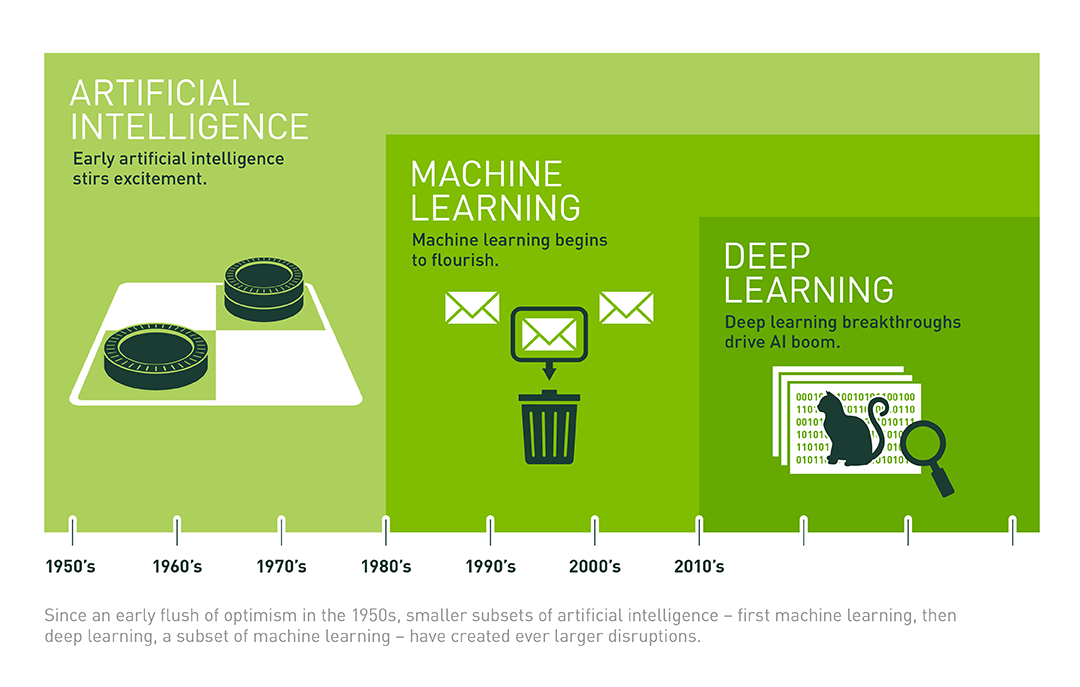
\includegraphics[width = \textwidth]{Chapters/00_loinoidau/dl.png}
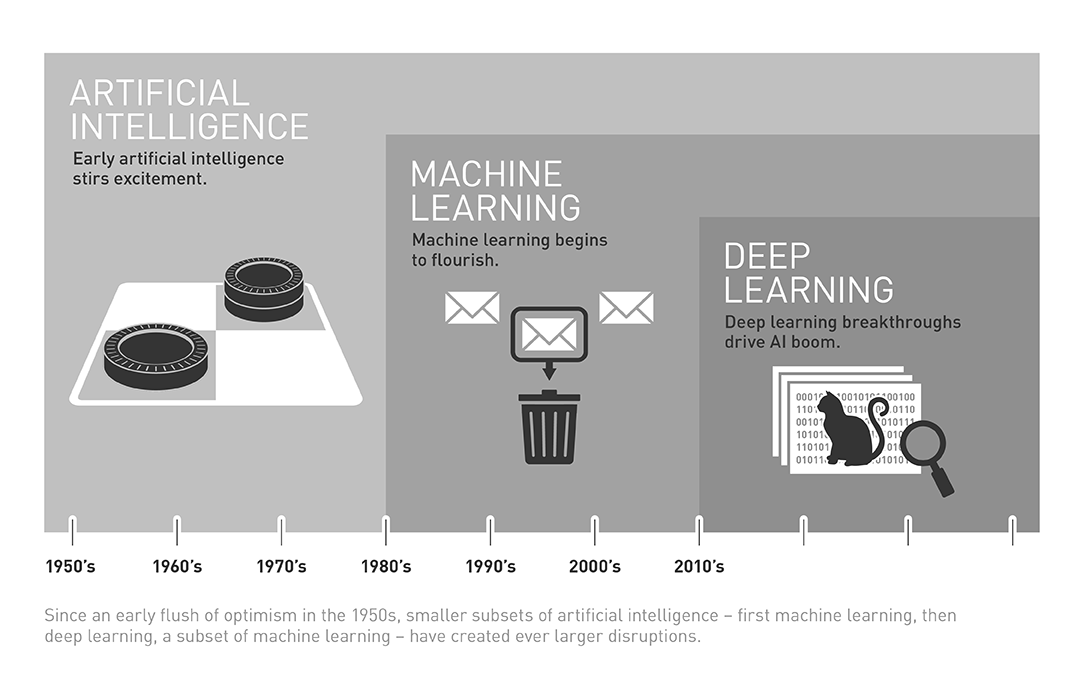
\includegraphics[width = .9\textwidth]{Chapters/00_loinoidau/dl_gray.png}
\caption[]{Mối quan hệ giữa AI, ML, và DL. (Nguồn \textit{What’s the Difference Between Artificial
Intelligence, Machine Learning, and Deep Learning?} --
\url{https://goo.gl/NNwGCi}).}
\label{fig:0_1}
\end{figure}
%% *****************************************************************************
\newnote{Mối quan hệ AI-ML-DL}{ DL là một tập con của ML. ML là một tập con của
AI (xem Hình~\ref{fig:0_1}). }

\section{Mục đích của cuốn sách}
Những phát triển thần kỳ của trí tuệ nhân tạo dẫn tới nhu cầu cao về mặt nhần
lực làm việc trong các ngành liên quan tới machine learning ở Việt Nam cũng như
trên thế giới. Đó cũng là nguồn động lực để tác giả gây dựng và phát triển
blog Machine Learning cơ bản từ đầu năm 2017
(\url{https://machinelearningcoban.com}). Tính tới thời điểm đặt bút viết những
dòng này, blog đã có hơn một triệu lượt ghé thăm. Facebook page Machine Learning
cơ bản\footnote{\url{https://goo.gl/wyUEjr}} chạm mốc 14 nghìn lượt likes, Forum
Machine Learning cơ bản\footnote{\url{https://goo.gl/gDPTKX}} đạt tới 17 nghìn
thành viên. Trong quá trình viết blog và duy trì các trang Facebook, tác giả đã
nhận được nhiều sự ủng hộ của bạn đọc về tinh thần cũng như vật chất. Nhiều
bạn đọc cũng khuyến khích tác giả tổng hợp kiến thức trên blog thành một
cuốn sách cho cộng đồng những người tiếp cận với ML bằng tiếng
Việt. Sự ủng hộ và những lời động viên đó là động lực lớn cho tác giả khi bắt
tay vào thực hiện và hoàn thành cuốn sách này.


Lĩnh vực ML nói chung và DL nói riêng là cực kỳ lớn và có nhiều nhánh nhỏ. Phạm vi
một cuốn sách chắc chắn không thể bao quát hết mọi vấn đề và đi sâu vào từng
nhánh cụ thể. Do vậy, cuốn sách này chỉ nhằm cung cấp cho bạn đọc những
khái niệm, kỹ thuật chung và các thuật toán cơ bản nhất của ML. Từ đó, bạn đọc
có thể tự tìm thêm các cuốn sách và khóa học liên quan nếu muốn đi sâu vào từng
vấn đề.



Hãy nhớ rằng \textit{luôn bắt đầu từ những điều đơn giản}. Khi bắt tay vào giải
quyết một bài toán ML hay bất cứ bài toán nào, chúng ta nên bắt đầu từ những
thuật toán đơn giản. Không phải chỉ có những thuật toán phức tạp mới có thể
giải quyết được vấn đề. Những thuật toán phức tạp thường có yêu cầu cao về khả
năng tính toán và đôi khi nhạy cảm với cách chọn tham số. Ngược lại, những
thuật toán đơn giản giúp chúng ta nhanh chóng có một bộ khung cho mỗi bài
toán. Kết quả của các thuật toán đơn giản cũng mang lại cái nhìn sơ bộ về sự
phức tạp của mỗi bài toán. Việc cải thiện kết quả sẽ được thực hiện dần ở các
bước sau. Cuốn sách này sẽ trang bị cho bạn đọc những kiến thức khái quát và một
số hướng tiếp cận cơ bản cho các bài toán ML. Để tạo ra các sản phẩm thực tiễn,
chúng ta cần học hỏi và thực hành thêm nhiều.


\section{Hướng tiếp cận của cuốn sách}

Để giải quyết mỗi bài toán ML, chúng ta cần chọn một mô hình phù hợp. Mô hình
này được mô tả bởi bộ các tham số mà chúng ta cần đi tìm. Thông thường, lượng
tham số có thể lên tới hàng triệu và được tìm bằng cách giải một bài toán tối
ưu.

Khi viết về các thuật toán ML, tác giả sẽ bắt đầu từ những ý tưởng trực quan.
Những ý tưởng này được mô hình hoá dưới dạng một bài toán tối ưu. Các suy luận
toán học và ví dụ mẫu trên Python ở cuối mỗi chương sẽ giúp bạn đọc hiểu rõ hơn
về nguồn gốc, ý nghĩa, và cách sử dụng mỗi thuật toán. Xen kẽ giữa những thuật
toán ML, tác giả sẽ trình bày các kỹ thuật tối ưu cơ bản, với hy vọng giúp bạn
đọc hiểu rõ hơn bản chất của vấn đề.
%%%%%%%%%%%%%%%%
\section{Đối tượng của cuốn sách}
Cuốn sách được thực hiện hướng tới nhiều nhóm độc giả khác nhau. Nếu bạn không
thực sự muốn đi sâu vào phần toán, bạn vẫn có thể tham khảo mã nguồn và cách sử
dụng các thư viện. Nhưng để sử dụng các thư viện một cách hiệu quả, bạn cũng cần
hiểu nguồn gốc của mô hình và ý nghĩa của các tham số. Còn nếu bạn thực sự muốn
tìm hiểu nguồn gốc, ý nghĩa của các thuật toán, bạn có thể học được nhiều điều
từ cách xây dựng và tối ưu các mô hình. Phần tổng hợp các kiến thức toán cần
thiết trong Phần~\ref{part:math} sẽ là một nguồn tham khảo súc tích bất cứ khi
nào bạn có thắc mắc về các dẫn giải toán học. Phần~\ref{part:cvxopt} được dành
riêng để nói về tối ưu lồi -- một mảng quan trọng trong tối ưu, phù hợp với các
bạn thực sự muốn đi sâu thêm về tối ưu.

Các dẫn giải toán học được xây dựng phù hợp với chương trình toán phổ thông và
đại học ở Việt Nam. Các từ khóa khi được dịch sang tiếng Việt đều dựa trên những
tài liệu tác giả được học trong nhiều năm tại Việt Nam.

Phần cuối cùng của sách có mục Index các thuật ngữ quan trọng và thuật ngữ tiếng Anh đi kèm giúp bạn dần làm quen khi đọc các tài liệu tiếng Anh.


\section{Yêu cầu về kiến thức}

Để có thể bắt đầu đọc cuốn sách này, bạn cần có một kiến thức nhất định về đại
số tuyến tính, giải tích ma trận, xác suất thống kê, và kỹ năng lập trình.

Phần~\ref{part:math} của cuốn sách ôn tập lại các kiến thức toán quan trọng được
dùng trong ML. Khi gặp khó khăn về toán, bạn được khuyến khích đọc lại các
chương trong phần này.

\index{numpy}
\index{scikit-learn}
\index{sklearn}
Ngôn ngữ lập trình được sử dụng trong cuốn sách là Python. Python là một ngôn
ngữ lập trình miễn phí, có thể được cài đặt dễ dàng trên các nền tảng hệ điều
hành khác nhau. Quan trọng hơn, có rất nhiều thư viện hỗ trợ ML cũng như DL
trên Python. Có hai thư viện Python chính thường được sử dụng trong
cuốn sách là numpy và scikit-learn.

Numpy (\url{http://www.numpy.org/}) là một thư viện phổ biến giúp xử lý các phép
toán liên quan đến các mảng nhiều chiều, hỗ trợ các hàm gần gũi với đại số tuyến
tính. Nếu bạn đọc chưa quen thuộc với numpy, bạn có thể tham gia một khóa học
ngắn miễn phí trên trang web kèm theo cuốn sách này (\url{https://fundaml.com}).
Bạn sẽ được làm quen với cách xử lý các mảng nhiều chiều với nhiều ví dụ và bài
tập thực hành. Các kỹ thuật xử lý mảng trong cuốn sách này đều được đề cập tại
đây.

Scikit-learn, hay sklearn (\url{http://scikit-learn.org/}), là một thư viện chứa
đầy đủ các thuật toán ML cơ bản và rất dễ sử dụng. Tài liệu của scikit-learn
cũng là một nguồn tham khảo chất lượng cho các bạn làm ML. Scikit-learn sẽ được
dùng trong cuốn sách để kiểm chứng các suy luận toán học và các mô hình được xây
dựng thông qua numpy.

Có rất nhiều thư viện giúp chúng ta tạo ra các sản phẩm ML/DL mà không yêu
cầu nhiều kiến thức toán. Tuy nhiên, cuốn sách này hướng tới việc giúp bạn đọc
hiểu bản chất toán học đằng sau mỗi mô hình trước khi áp dụng các thư viện sẵn
có. Việc sử dụng thư viện cũng yêu cầu kiến thức nhất định về việc lựa chọn mô
hình và điều chỉnh các tham số.
%%%%%%%%%%%%%%%%%%%%%%%%%
\section{Mã nguồn đi kèm}
Toàn bộ mã nguồn trong cuốn sách có thể được tìm thấy tại
\url{https://goo.gl/Fb2p4H}. Các file có đuôi \texttt{.ipynb} là các
Jupyter notebook chứa mã nguồn. Các file có đuôi \texttt{.pdf}, và \texttt{.png}
là các hình vẽ được sử dụng trong cuốn sách.

\section{Bố cục của cuốn sách}
Cuốn sách này được chia thành 8 phần và sẽ tiếp tục được cập nhật:

{Phần~\ref{part:math}} ôn tập lại những kiến thức quan trọng trong đại số tuyến
tính, giải tích ma trận, xác suất, và hai phương pháp phổ biến trong việc ước
lượng tham số cho các mô hình ML dựa trên thống kê.

Phần~\ref{part:overview} giới thiệu các khái niệm cơ bản trong ML, các kỹ thuật
xây dựng vector đặc trưng cho dữ liệu, một mô hình ML cơ bản -- hồi quy, và một hiện tượng cần tránh khi xây dựng các mô hình ML.

Phần~\ref{part:warmup} giúp các bạn làm quen với các mô hình ML không yêu cầu
nhiều kiến thức toán phức tạp. Qua đây, bạn đọc sẽ có cái nhìn sơ bộ về việc xây
dựng các mô hình ML.


Phần~\ref{part:neuralnets} đề cập tới một nhóm các thuật toán ML phổ biến nhất
-- mạng neuron nhân tạo, là nền tảng cho các mô hình DL phức tạp
hiện nay. Phần này cũng giới thiệu một kỹ thuật tối ưu phổ biến cho các bài toán
tối ưu không ràng buộc.

Phần~\ref{part:recsys} giới thiệu về các kỹ thuật thường dùng trong các hệ thống
gợi ý sản phẩm.

Phần~\ref{part:dimred} giới thiệu các kỹ thuật giảm chiều dữ liệu.

Phần~\ref{part:cvxopt} trình bày cụ thể hơn về tối ưu, đặc biệt là tối ưu lồi.
Các bài toán tối ưu lồi có ràng buộc cũng được giới thiệu trong phần này.

Phần~\ref{par:svm} giới thiệu các thuật toán phân loại dựa trên máy vector hỗ trợ.


\section{Các lưu ý về ký hiệu}
Các ký hiệu toán học trong sách được mô tả ở Bảng~\ref{tab:notation} và đầu
Chương~\ref{cha:linearalgebra}.
% Ngoài ra, các font chữ khác nhau cũng được sử dụng với các mục đích khác nhau:
Các khung với font chữ có cùng chiều rộng được dùng để chứa các đoạn mã nguồn.
\begin{lstlisting}
text in a box with constant width represents source codes.
\end{lstlisting}
Các đoạn ký tự với \pythoninline{constant width} (có cùng chiều rộng)
được dùng để chỉ các biến, hàm số, chuỗi,...  trong các đoạn mã.
\newnote{Đóng khung và in nghiêng}{
Các khái niệm, định nghĩa, định lý, và lưu ý quan trọng được đóng khung và
in nghiêng.

Ký tự phân cách giữa phần nguyên và phần thập phân của các số thực là dấu
chấm (.) thay vì dấu phẩy (,) như trong các tài liệu tiếng Việt khác.
Cách làm này thống nhất với các tài liệu tiếng Anh và các ngôn
ngữ lập trình.
}


\section{Tham khảo thêm}

Có nhiều cuốn sách, khóa học, website hay về machine learning/deep learning. Trong đó, tôi xin đặc biệt nhấn mạnh các nguồn tham khảo sau:

\subsection{Khoá học}
\begin{enumerate}
\item Khoá học \textit{Machine Learning} của Andrew Ng trên Coursera
(\url{https://goo.gl/WBwU3K}).

\item Khoá học mới \textit{Deep Learning Specialization} cũng của Andrew Ng
trên Coursera (\url{https://goo.gl/ssXfYN}).

\item Các khóa \textit{CS224n: Natural Language Processing with Deep
Learning} (\url{https://goo.gl/6XTNkH}); \textit{CS231n: Convolutional Neural
Networks for Visual Recognition} (\url{http://cs231n.stanford.edu/});
\textit{CS246: Mining Massive Data Sets} (\url{https://goo.gl/TEMQ9H}) của
Stanford.

%   \item \textit{Introduction to Computer Science and Programming Using Python}
%   (\url{https://goo.gl/4nNXvJ}) của MIT.

\end{enumerate}

\subsection{Sách}
\begin{enumerate}

\item  C. Bishop, \textit{Pattern Recognition and Machine
Learning} (\url{https://goo.gl/pjgqRr}), Springer,
2006~\cite{bishop2006pattern}.

\item I. Goodfellow \etal,
\textit{Deep Learning} (\url{https://goo.gl/sXaGwV}), MIT press,
2016~\cite{Goodfellow-et-al-2016}.

\item J. Friedman \etal, \textit{The Elements of Statistical
Learning} (\url{https://goo.gl/Qh9EkB}), Springer, 2001~\cite{friedman2001elements}.


\item Y. Abu-Mostafa \etal, \textit{Learning from data}
(\url{https://goo.gl/SRfNFJ}), AMLBook New York,
2012~\cite{abu2012learning}.

\item S. JD Prince, \textit{Computer Vision: Models, Learning, and
Inference} (\url{https://goo.gl/9Fchf3}), Cambridge University Press,
2012~\cite{prince2012computer}.

\item S. Boyd \etal, \textit{Convex Optimization}
(\url{https://goo.gl/NomDpC}), Cambridge university
press, 2004~\cite{boyd2004convex}.

\end{enumerate}
Ngoài ra, các website \textit{Machine Learning Mastery}
(\url{https://goo.gl/5DwGbU}), \textit{Pyimagesearch}
(\url{https://goo.gl/5DwGbU}). \textit{Kaggle} (\url{https://www.kaggle.com/}),
\textit{Scikit-learn} (\url{http://scikit-learn.org/}) cũng là các nguồn thông
tin hữu ích.

\section{Đóng góp ý kiến}
Các bạn có thể gửi các đóng góp tới địa chỉ email \textit{vuhuutiep@gmail.com}
hoặc tạo một \textit{GitHub issue} mới tại \url{https://goo.gl/zPYWKV}.

% \section{Vấn đề bản quyền}
% Toàn bộ nội dung trên blog cũng như cuốn sách này (bao gồm cả source code và
% hình ảnh minh hoạ) đều thuộc bản quyền của tôi  --  Vũ Hữu Tiệp.

% Tôi rất mong muốn kiến thức của mình tạo ra đến được với nhiều bạn đọc. Tuy
% nhiên, tôi không ủng hộ bất kỳ một hình thức sao chép không trích nguồn nào. Mọi
% trích dẫn cần được nêu rõ tên cuốn sách, tên tác giả (Vũ Hữu Tiệp), và link gốc
% tới blog. Các bài viết trích dẫn quá 25\% toàn văn bất kỳ một post nào trên
% blog hoặc một chương trong cuốn sách này đều không được phép, trừ trường hợp có
% sự đồng ý của tác giả.

% Mọi vấn đề liên quan đến sao chép, phân phát, đăng tải, sử dụng sách và blog,
% cũng như trao đổi, cộng tác, xin vui lòng liên hệ với tôi tại địa chỉ email
% vuhuutiep@gmail.com.



% \newpage
\section{Lời cảm ơn}
Trước hết, tôi xin được cảm ơn sự ủng hộ và chia sẻ nhiệt tình của bạn bè trên  Facebook từ những ngày đầu ra mắt blog. Xin được gửi lời cảm ơn chân thành tới bạn đọc Machine Learning cơ bản đã đồng hành trong hơn một năm qua.

Tôi cũng may mắn nhận được những góp ý và phản hồi tích cực từ các thầy cô
tại các trường đại học lớn trong và ngoài nước. Xin phép được gửi lời cảm ơn
tới thầy Phạm Ngọc Nam và cô Nguyễn Việt Hương (ĐH Bách Khoa Hà Nội), thầy Chế
Viết Nhật Anh (ĐH Bách Khoa TP.HCM), thầy Nguyễn Thanh Tùng (ĐH Thuỷ Lợi),
và thầy Trần Duy Trác (ĐH Johns Hopkins).

Đặc biệt, xin cảm ơn Nguyễn Hoàng Linh và Hoàng Đức Huy, Đại học Waterloo,
Canada đã nhiệt tình giúp tôi xây dựng trang \url{FundaML.com}, cho phép độc giả
học Python/Numpy trực tiếp trên trình duyệt. Xin cảm ơn các bạn Nguyễn
Tiến Cường, Nguyễn Văn Giang, Vũ Đình Quyền, Lê Việt Hải, và Đinh Hoàng Phong đã
góp ý sửa đổi nhiều điểm trong các bản nháp.

Ngoài ta, cũng xin cảm ơn những người bạn thân của tôi tại Penn State
(ĐH bang Pennsylvania) đã luôn bên cạnh tôi trong thời gian tôi thực hiện dự án,
bao gồm gia đình anh Triệu Thanh Quang, gia đình anh Trần Quốc Long, bạn thân
Nguyễn Phương Chi, và các đồng nghiệp tại Phòng nghiên cứu Xử lý Thông tin và
Thuật toán (Information Processing and Algorithm Laboratory, iPAL).

Cuối cùng và quan trọng nhất, xin gửi lời cảm ơn sâu sắc nhất tới gia đình tôi,
những người luôn ủng hộ vô điều kiện và hỗ trợ tôi hết mình trong quá trình thực
hiện dự án này.
%!TEX root = ../book_ML.tex

\def\R{\mathbb{R}}
\section{Bảng các ký hiệu}
Các ký hiệu sử dụng trong sách được liệt kê trong Bảng~\ref{tab:notation} ở trang tiếp theo. 

\begin{table}[h]
    \caption{Các quy ước ký hiệu và tên gọi được sử dụng trong sách}
    \label{tab:notation}
    \centering
    \begin{tabular}{|c|l|}
    \hline 
    Ký hiệu & Ý nghĩa  \\ \hline 
    \hline 
    $x, y, N, k$ & in nghiêng, thường hoặc hoa, là các số vô hướng \\ \hline
    $\bx, \by$ & in đậm, chữ thường, là các vector  \\ \hline
    $\bX, \bY$ & in đậm, chữ hoa, là các ma trận  \\ \hline
    $\R$ & tập hợp các số thực \\ \hline 
    $\mathbb{N}$ & tập hợp các số tự nhiên \\ \hline 
    $\mathbb{C}$ & tập hợp các số phức \\ \hline 
    $\R^{m}$ & tập hợp các vector thực có $m$ phần tử \\ \hline 
    $\R^{m\times n}$ &tập hợp các ma trận thực có $m$ hàng, $n$ cột \\ \hline
    $\mathbb{S}^n$ & tập hợp các ma trận vuông đối xứng bậc $n$ \\ \hline 
    $\mathbb{S}^n_{+}$ & tập hợp các ma trận nửa xác định dương bậc $n$ \\
    \hline 
    $\mathbb{S}^n_{++}$ & tập hợp các ma trận xác định dương bậc $n$ \\ \hline 
    $ \in $ & phần tử thuộc tập hợp \\ \hline 
    $ \exists $ & tồn tại \\ \hline 
    $ \forall $ & mọi \\ \hline 
    $ \triangleq$ & ký hiệu là/bởi. Ví dụ $a\triangleq f(x)$ nghĩa là ``ký hiệu
    $f(x)$ bởi $a$''. \\ \hline 
    $x_i$ & phần tử thứ $i$ (tính từ 1) của vector $\bx$ \\ \hline 
    $\sgn(x)$ & hàm xác định dấu. Bằng 1 nếu $x \geq 0$, bằng -1 nếu $x < 0$. \\ \hline
    $\exp(x)$ & $e^x$ \\ \hline
    $\log(x)$ & logarit \textit{tự nhiên} của số thực dương $x$ \\ \hline
    $\displaystyle \argmin_xf(x)$ & giá trị của $x$ để hàm $f(x)$ đạt giá trị nhỏ nhất \\ \hline 
    $\displaystyle \argmax_xf(x)$ & giá trị của $x$ để hàm $f(x)$ đạt giá trị lớn nhất \\ \hline 
    $a_{ij}$ & phần tử hàng thứ $i$, cột thứ $j$ của ma trận $\bA$ \\ \hline 
    $\bA^T$ & chuyển vị của ma trận $\bA$ \\ \hline 
    $\bA^H$ & chuyển vị liên hợp (Hermitian) của ma trận phức $\bA$ \\ \hline 
    $\bA^{-1}$ & nghịch đảo của ma trận vuông $\bA$, nếu tồn tại \\ \hline 
    $\bA^{\dagger}$ & giả nghịch đảo của ma trận không nhất thiết vuông $\bA$ \\
    \hline 
    $\bA^{-T}$ & chuyển vị của nghịch đảo của ma trận $\bA$, nếu tồn tại \\ \hline 
    $\|\bx\|_p$ & $\ell_p$ norm của vector $\bx$ \\ \hline  
    $\|\bA\|_F$ &  Frobenius norm của ma trận $\bA$ \\ \hline 
    $ \diag(\bA)$ & đường chéo chính của ma trận $\bA$ \\ \hline 
    $\trace(\bA)$ & trace của ma trận $\bA$ \\ \hline 
    $\det(\bA)$ & định thức của ma trận vuông $\bA$ \\ \hline 
    $\text{rank}(\bA)$ & hạng của ma trận $\bA$ \\ \hline 
    o.w & \textit{otherwise}  --  trong các trường hợp còn lại \\ \hline 
    $\displaystyle\frac{\partial f}{\partial x}$ & đạo hàm của hàm số $f$ theo $x \in \R$ \\ \hline
    $\nabla_{\bx}f$ & gradient của hàm số $f$ theo $\bx$ ($\bx$ là vector hoặc ma trận) \\ \hline 
    $\nabla^2_{\bx}f$ & gradient bậc hai của hàm số $f$ theo $\bx$, còn được gọi là \textit{Hesse} \\ \hline 
    $\odot$ & \makecell{Hadamard product (elemenwise product). Phép nhân từng phần tử \\ của hai vector hoặc ma trận cùng kích thước.} \\ \hline 
    $\propto$ & tỉ lệ với \\ \hline 
    % v.v. & vân vân \\ \hline 
    %%%%%%%
    \begin{tikzpicture}
    \draw [thick] (0, 0) -- (1, 0); 
    \end{tikzpicture}
    & đường nét liền \\ \hline 

    %%%%%%%
    \begin{tikzpicture}
    \draw [very thick, dashed] (0, 0) -- (1, 0); 
    \end{tikzpicture}
    & đường nét đứt \\ \hline 

    %%%%%%%
    \begin{tikzpicture}
    \draw [very thick, dotted] (0, 0) -- (1, 0); 
    \end{tikzpicture}
    & đường nét chấm (đường chấm chấm)\\ \hline 

    %%%%%%%
    \begin{tikzpicture}
    \draw [very thick, dash pattern={on 7pt off 2pt on 1pt off 3pt}] (0,0) -- (1,0);
    \end{tikzpicture}
    & đường chấm gạch\\ \hline 
    %%%%%%%
    % \\[-3mm]
    % \vspace{1em}
    \begin{tikzpicture}[yshift = -1cm]
    \draw [pattern = dots] (0,0) rectangle (1,.4);
    \end{tikzpicture}
    & nền chấm\\\hline 
    %%%%%%%
    % \\[-1em]
    % \vspace{1em}
    \begin{tikzpicture}
    \draw [pattern = custom north west lines] (0,0) rectangle (1,.4);
    \end{tikzpicture}
    & nền sọc chéo\\ \hline 



    \end{tabular}
 \end{table} 




% Nhu cầu về nhân lực ngành Machine Learning (Deep Learning) đang ngày một cao, kéo theo đó nhu cầu học Machine Learning trên thế giới và ở Việt Nam ngày một lớn. Cá nhân tôi cũng muốn hệ thống lại kiến thức của mình về lĩnh vực này để chuẩn bị cho tương lai (đây là một trong những mục tiêu của tôi trong năm 2017). Tôi sẽ cố gắng đi từ những thuật toán cơ bản nhất của Machine Learning kèm theo các ví dụ và mã nguồn trong mỗi bài viết. Tôi sẽ viết 1-2 tuần 1 bài (việc viết các công thức toán và code trên blog thực sự tốn nhiều thời gian hơn tôi từng nghĩ). Đồng thơi, tôi cũng mong muốn nhận được phản hồi của bạn đọc để qua những thảo luận, tôi và các bạn có thể nắm bắt được các thuật toán này.

% Khi chuẩn bị các bài viết, tôi sẽ giả định rằng bạn đọc có một chút kiến thức về Đại Số Tuyến Tính (Linear Algebra), Xác Suât Thống Kê (Probability and Statistics) và có kinh nghiệm về lập trình Python. Nếu bạn chưa có nhiều kinh nghiệm về các lĩnh vực này, đừng quá lo lắng vì mỗi bài sẽ chỉ sử dụng một vài kỹ thuật cơ bản. Hãy để lại câu hỏi của bạn ở phần Comment bên dưới mỗi bài, tôi sẽ thảo luận thêm với các bạn.

% Trong bài tiếp theo của blog này, tôi sẽ giới thiệu về các nhóm thuật toán Machine Learning cơ bản. Mời các bạn theo dõi.

% \section{Tham khảo thêm}
% \subsection{Các khóa học}
% \subsubsection{Tiếng Anh}
% \begin{enumerate}
% 	\item \href{https://www.coursera.org/learn/machine-learning}{Machine Learning với thầy Andrew Ng trên Coursera} ({\it Khóa học nổi tiếng nhất về Machine Learning })

% 	\item \href{https://www.udacity.com/course/deep-learning -- ud730}{Deep Learning by Google trên Udacity} ({\it Khóa học nâng cao hơn về Deep Learning với Tensorflow})


% 	\item \href{http://machinelearningmastery.com/}{Machine Learning mastery} ({\it Các thuật toán Machine Learning cơ bản})
% \end{enumerate}

% \subsubsection{Tiếng Việt}
% {\bf Lưu ý}: {\it Các khóa học này tôi chưa từng tham gia, chỉ đưa ra để các bạn tham khảo.}
% \begin{enumerate}
% 	\item \href{http://tuanvannguyen.blogspot.com/2016/12/cap-nhat-khoa-hoc-ve-machine-learning.html}{Machine Learning 1/2017}


% 	\item \href{https://techmaster.vn/khoa-hoc/25511/machine-learning-co-ban}{Nhập môn Machine Learning, Tech Master- Cao Thanh Hà {\it POSTECH}}()

% \end{enumerate}

% \subsection{Các trang Machine Learning tiếng Việt khác}
% \begin{enumerate}
% 	\item \href{http://viet.jnlp.org/kien-thuc-co-ban-ve-xu-ly-ngon-ngu-tu-nhien/machine-learning-trong-nlp}{Machine Learning trong Xử Lý Ngôn Ngữ Tự Nhiên - Nhóm Đông Du {\it Nhật Bản}}

% 	\item \href{https://ongxuanhong.wordpress.com/}{Machine Learning cho người mới bắt đầu - Ông Xuân Hồng {\it JAIST}}.


% 	 \item \href{https://ml-book-vn.khanhxnguyen.com/}{Machine Learning book for Vietnamese - Nguyễn Xuân Khánh \textit{University of Maryland}}
% \end{enumerate}
% 3. [Machine Learning trong Xử Lý Ngôn Ngữ Tự Nhiên - Nhóm Đông Du _Nhật Bản_](http://viet.jnlp.org/kien-thuc-co-ban-ve-xu-ly-ngon-ngu-tu-nhien/machine-learning-trong-nlp)
% 4. [Machine Learning cho người mới bắt đầu - Ông Xuân Hồng _JAIST_](https://ongxuanhong.wordpress.com/).
% 5. [Machine Learning book for Vietnamese - Nguyễn Xuân Khánh _University of Maryland_](https://ml-book-vn.khanhxnguyen.com/)


\part{Kiến thức toán cơ bản}
\label{part:math}

\setcounter{chapter}{0}
% !TEX root = ../../book_ML.tex
\chapter{Ôn tập Đại số tuyến tính}
\label{cha:linearalgebra}

\section{Lưu ý về ký hiệu}

Trong cuốn sách này, những số vô hướng được biểu diễn bởi các chữ cái
in nghiêng và có thể viết hoa, ví dụ $x_1, N, y, k$. Các ma trận được biểu diễn
bởi các chữ viết hoa in đậm, ví dụ $\mathbf{X, Y, W} $. Các vector được biểu
diễn bởi các chữ cái thường in đậm, ví dụ $\mathbf{y}, \mathbf{x}_1 $. Nếu
không giải thích gì thêm, các vector được mặc định hiểu là các vector cột.

Đối với vector, $\mathbf{x} = [x_1, x_2, \dots, x_n]$ được hiểu là một vector
hàng, $\mathbf{x} = [x_1; x_2; \dots; x_n] $ được hiểu là vector cột. Chú ý
sự khác nhau giữa dấu phẩy ($,$) và dấu chấm phẩy ($;$). Đây chính là ký hiệu
được Matlab sử dụng. Nếu không giải thích gì thêm, một chữ cái viết thường in
đậm được hiểu là một vector cột.

Tương tự, trong ma trận, $\mathbf{X} = [\mathbf{x}_1, \mathbf{x}_2, \dots,
\mathbf{x}_n]$ được hiểu là các vector cột $\mathbf{x}_j$ được đặt cạnh nhau
theo thứ tự từ trái qua phải để tạo ra ma trận $\mathbf{X}$. Trong khi
$\mathbf{X} = [\mathbf{x}_1; \mathbf{x}_2; \dots; \mathbf{x}_m]$ được hiểu là
các vector $\mathbf{x}_i$ được đặt chồng lên nhau theo thứ tự từ trên xuống dưới
dể tạo ra ma trận $\mathbf{X}$. Các vector được ngầm hiểu là có kích thước phù
hợp để có thể xếp cạnh hoặc xếp chồng lên nhau. Phần tử ở hàng thứ $i$, cột thứ
$j$ được ký hiệu là $x_{ij}$.

% \textit{Chú ý: Một số tài liệu có sử dụng ký hiệu khác như sau. Cho một ma
% trận $\bX \in \R^{m \times n}$, cột thứ $i$ của ma trận được ký hiệu là
% $\bX_{:,i}$; hàng thứ $j$ của ma rận được ký hiệu là $\bX_{j,:}$; phần tử ở hàng
% thứ $i$, cột thứ $j$ được ký hiệu là $X_{i,j}$. Khi đọc, chúng ta cần chú ý các
% ký hiệu toán học. }

Cho một ma trận $\mathbf{W}$, nếu không giải thích gì thêm, ta hiểu rằng
$\mathbf{w}_i$ là \textbf{vector cột} thứ $i$ của ma trận đó. Chú ý sự tương ứng
giữa ký tự viết hoa và viết thường.


% section chuyen_vi (end)
% \newpage
% \index{chuyển vị}
\section{Chuyển vị và Hermitian} % (fold)
\label{sec:chuyen_vi}


% Một phép toán quan trọng trong đại số tuyến tính là \textit{chuyển vị}
% (\textit{transpose}).
\index{chuyển vị -- transpose}
\index{transpose -- chuyển vị}
Cho một ma trận/vector $\bA \in \R^{m\times n}$, ta nói $\bB \in \R^{n\times m}$ là \textit{chuyển vị} (transpose) của
$\bA$ nếu $b_{ij} = a_{ji},~\forall 1 \leq i \leq n, 1 \leq j\leq m$.

Chuyển vị của ma trận $\bA$ được ký hiệu là $\bA^T$. Cụ thể hơn:
\begin{eqnarray*}
\bx = \left[
\begin{matrix}
x_1 \\ x_2 \\ \vdots \\ x_m
\end{matrix}
\right] \Rightarrow \bx^T = \left[
\begin{matrix}
x_1 & x_2 & \dots & x_m
\end{matrix}
\right];
\end{eqnarray*}
\begin{eqnarray*}
\bA = \left[
\begin{matrix}
a_{11} & a_{12} & \dots & a_{1n} \\
a_{21} & a_{22} & \dots & a_{2n} \\
% a_{31} & a_{32} & \dots & a_{3n} \\
\dots & \dots & \ddots & \dots \\
a_{m1} & a_{m2} & \dots & a_{mn}
\end{matrix}
\right]
\Rightarrow
\bA^T = \left[
\begin{matrix}
a_{11} & a_{21}  &\dots & a_{m1} \\
a_{12} & a_{22}  & \dots & a_{m2} \\
\dots & \dots &  \ddots & \dots \\
a_{1n} & a_{2n} & \dots & a_{mn}
\end{matrix}
\right]
\end{eqnarray*}
% \begin{eqnarray}
% \bA = \left[
% \begin{matrix}
%     a_{11} & a_{12} & \dots & a_{1n} \\
%     a_{21} & a_{22} & \dots & a_{2n} \\
%     % a_{31} & a_{32} & \dots & a_{3n} \\
%     \dots & \dots & \ddots & \dots \\
%     a_{m1} & a_{m2} & \dots & a_{mn}
% \end{matrix}
% \right]
% \Rightarrow
% \bA^T = \left[
% \begin{matrix}
% a_{11} & a_{21}  &\dots & a_{m1} \\
% a_{12} & a_{22}  & \dots & a_{m2} \\
% \dots & \dots &  \ddots & \dots \\
% a_{1n} & a_{2n} & \dots & a_{mn}
% \end{matrix}
% \right]
% \end{eqnarray}
% \sec{Tích Hadamard của hai ma trận}
% \label{sec:Hamard}

Nếu $\bA \in \R^{m\times n}$ thì $\bA^T \in \R^{n\times m}$. Nếu $\bA^T = \bA$, ta
nói $\bA$ là một \textit{ma trận đối xứng}.

\index{ma trận đối xứng -- symmetric matrix}
\index{symmetric matrix -- ma trận đối xứng}
\index{Hermitian}
\index{chuyển vị liên hợp -- conjugate transpose}
\index{conjugate transpose -- chuyển vị liên hợp}
Trong trường hợp vector hay ma trận có các phần tử là số phức, việc lấy chuyển
vị thường đi kèm với việc lấy liên hợp phức. Tức là ngoài việc đổi vị trí của
các phần tử, ta còn lấy liên hợp phức của các phần tử đó. Tên gọi của phép toán
chuyển vị và lấy liên hợp này còn được gọi là \textit{chuyển vị liên hợp} (conjugate transpose), và
thường được ký hiệu bằng chữ $H$ thay cho chữ $T$. Chuyển vị liên hợp của một ma
trận $\bA$ được ký hiệu là $\bA^H$, được đọc là $\bA$ Hermitian.

Cho $\bA \in \mathbb{C}^{m\times n}$, ta nói $\bB \in \mathbb{C}^{n\times m}$ là chuyển vị liên
hợp của $\bA$ nếu
$b_{ij} = \lbar{a_{ji}},~\forall 1 \leq i \leq n, 1 \leq j \leq m$,
trong đó $\lbar{a}$ là liên hiệp phức của $a$.

\textit{Ví dụ}:
\begin{equation}
\bA = \bmt 1 + 2i &~~ & 3 - 4i \\
i &~~ & 2 \emt
\Rightarrow \bA^{H} =
\bmt 1 - 2i &~~ & -i \\
3 + 4i &~~ & 2 \emt
\end{equation}

Nếu $\bA, \bx$ là các ma trận và vector thực thì $\bA^H = \bA^T, \bx^H = \bx^T$.



Nếu chuyển vị liên hợp của một ma trận vuông phức bằng với chính nó, $\bA^H = \bA$,
ta nói ma trận đó là \textit{Hermitian}.


\section{Phép nhân hai ma trận} % (fold)
\label{sec:nhan_hai_ma_tran}
Cho hai ma trận $\bA \in \R^{m\times n}, \bB \in \R^{n \times p}$, tích của hai
ma trận được ký hiệu là $\bC = \bA\bB \in \R^{m \times p}$ trong đó phần tử ở
hàng thứ $i$, cột thứ $j$ của ma trận kết quả được tính bởi:
\begin{equation}
c_{ij} = \sum_{k=1}^na_{ik}b_{kj}, ~\forall 1\leq i \leq m, 1 \leq j \leq p
\end{equation}
Để nhân được hai ma trận, số cột của ma trận thứ nhất phải bằng số hàng của ma trận thứ hai. Trong ví dụ trên, chúng đều bằng $n$.

Giả sử kích thước các ma trận là phù hợp để các phép nhân ma trận tồn tại, ta có
một vài tính chất sau:

\begin{enumerate}

\item Phép nhân ma trận không có tính chất giao hoán. Thông thường (không
phải luôn luôn), $\bA\bB \neq \bB\bA$. Thậm chí, trong nhiều trường hợp, các
phép tính này không tồn tại vì kích thước các ma trận lệch nhau.

\item Phép nhân ma trận có tính chất kết hợp: $\bA \bB\bC = (\bA\bB)\bC = \bA(\bB\bC)$.
% \begin{equation}
% \bA \bB\bC = (\bA\bB)\bC = \bA(\bB\bC)
% \end{equation}

\item Phép nhân ma trận có tính chất phân phối đối với phép cộng: $\bA(\bB + \bC) = \bA\bB + \bA\bC$.
% \begin{equation}
%     \bA(\bB + \bC) = \bA\bB + \bA\bC
% \end{equation}

\item Chuyển vị của một tích bằng tích các chuyển vị theo thứ tự ngược lại.
Điều tương tự xảy ra với Hermitian của một tích:
\begin{equation}
(\bA\bB)^T = \bB^T \bA^T; \quad (\bA\bB)^H = \bB^H\bA^H
\end{equation}

\end{enumerate}
\index{tích vô hướng -- inner product}
\index{inner product -- tích vô hướng}
\index{trực giao -- orthogonal}
\index{orthogonal -- trực giao}
\textit{Tích trong}, hay \textit{tích vô hướng} (inner product) của hai vector $\bx, \by \in \R^n$
được định nghĩa bởi:
\begin{equation}
\bx^T\by = \by^T\bx = \sum_{i =1}^n x_iy_i
\end{equation}
Nếu tích vô hướng của hai vector khác không bằng không, ta nói hai vector đó
\textit{trực giao} (orthogonal).

Chú ý, $\bx^H\by$ và $\by^H\bx$ bằng nhau khi và chỉ khi
chúng là các số thực.

$\bx^H\bx \geq 0,~\forall\bx \in \mathbb{C}^n$ vì tích của một số phức với liên
hiệp của nó luôn là một số không âm.



Phép nhân của một ma trận $\bA \in \R^{m \times n}$ với một vector
$\bx \in \R^{n}$ là một vector $\bb \in \R^{m}$:
\begin{equation}
\bA\bx = \bb, ~\text{với} ~b_i = \bA_{i,:}\bx
\end{equation}
với $\bA_{i,:}$ là vector hàng thứ $i$ của $\bA$.

\index{phép nhân từng thành phần -- Hadamard product}
\index{Hadamard product -- phép nhân từng thành phần}
Ngoài ra, có một phép nhân khác được gọi là
\textit{phép nhân từng thành phần} hay \textit{tích Hadamard} (Hadamard product) thường xuyên được sử dụng trong machine learning. Tích Hadamard
của hai ma trận {cùng kích thước} $\bA, \bB \in \R^{m\times n}$, được ký hiệu là
$\bC = \bA \odot \bB \in \R^{m \times n}$, trong đó:
\begin{equation}
c_{ij} = a_{ij}b_{ij}
\end{equation}

\section{Ma trận đơn vị và ma trận nghịch đảo}
\label{sec:identitmatrix}
\subsection{Ma trận đơn vị} % (fold)
\label{sub:identity matrix }


\textit{Đường chéo chính} của một ma trận là tập hợp các điểm có chỉ số hàng và
cột bằng nhau. Cách định nghĩa này cũng có thể được áp dụng cho một ma trận
không vuông. Cụ thể, nếu $\bA \in \R^{m \times n}$ thì đường chéo chính của
$\bA$ bao gồm $\{a_{11}, a_{22}, \dots, a_{pp}\}$, trong đó $p = \min\{m, n\}$.

% subsection identity matrix  (end)
\index{identity matrix - ma trận đơn vị}
Một ma trận đơn vị bậc $n$ là một ma trận đặc biệt trong $\R^{n\times n}$ với
các phần tử trên đường chéo chính bằng 1, các phần tử còn lại bằng 0. Ma trận
đơn vị thường được ký hiệu là $\bI$. Khi làm việc với nhiều ma trận đơn vị với
bậc khác nhau, ta thường ký kiệu $\bI_n$ cho ma trận đơn vị bậc $n$. Dưới đây là
các ma trận đơn vị bậc 3 và bậc 4:
\begin{equation}
\bI_3 = \bmt
1 & 0 & 0 \\
0 & 1 & 0 \\
0 & 0 & 1
\emt, \quad
\bI_4 = \bmt
1 & 0 & 0 & 0\\
0 & 1 & 0 & 0 \\
0 & 0 & 1 & 0 \\
0 & 0 & 0 & 1
\emt
\end{equation}
Ma trận đơn vị có một tính chất đặc biệt trong phép nhân. Nếu $\bA \in
\R^{m\times n}$, $\bB \in \R^{n\times m}$ và $\bI$ là ma trận đơn vị bậc $n$, ta
có: $\bA\bI= \bA, \quad \bI\bB = \bB$.

Với mọi vector $\bx \in \R^n$, ta có $\bI_n \bx = \bx$.



\subsection{Ma trận nghịch đảo} % (fold)
\label{sub:inverse_matrix}
\index{inverse matrix - ma trận nghịch đảo}

Cho một ma trận vuông $\bA \in \R^{n\times n }$, nếu tồn tại một ma trận vuông
$\bB \in \R^{n\times n}$ sao cho $\bA\bB = \bI_n$, ta nói $\bA$ là \textit{khả
nghịch}, và $\bB$ được gọi là \textit{ma trận nghịch đảo} của $\bA$. Nếu không
tồn tại ma trận $\bB$ thoả mãn điều kiện trên, ta nói rằng ma trận $\bA$ là
{không khả nghịch}.

Nếu $\bA$ khả nghịch, ma trận nghịch đảo của nó được ký hiệu là $\bA^{-1}$. Ta
cũng có:
\begin{equation}
\bA^{-1}\bA = \bA\bA^{-1} = \bI
\end{equation}
% \begin{equation}
%     \bI_n \bx = \bx
% \end{equation}
Ma trận nghịch đảo thường được sử dụng để giải hệ phương trình tuyến tính. Giả
sử $\bA \in \R^{n\times n}$ là một ma trận khả nghịch và $\bb$ là một vector bất kỳ trong $\R^n$. Khi đó, phương trình:
\begin{equation}
\label{eqn:lin_eqn}
\bA\bx = \bb
\end{equation}
có nghiệm duy nhất $\bx = \bA^{-1}\bb$. Thật vậy, nhân bên trái cả hai vế của
phương trình với $\bA^{-1}$, ta có $\bA\bx = \bb \Leftrightarrow  \bA^{-1}\bA\bx = \bA^{-1}\bb \Leftrightarrow \bx = \bA^{-1}\bb$.
% \begin{equation}
%       \bA\bx = \bb \Leftrightarrow  \bA^{-1}\bA\bx = \bA^{-1}\bb \Leftrightarrow \bx = \bA^{-1}\bb
% \end{equation}

Nếu $\bA$ không khả nghịch, thậm chí không vuông, phương trình tuyến tính
\eqref{eqn:lin_eqn} có thể không có nghiệm hoặc có vô số nghiệm.

Giả sử các ma trận vuông $\bA, \bB$ là khả nghịch, khi đó tích của chúng cũng
khả nghịch, và $(\bA\bB)^{-1} = \bB^{-1}\bA^{-1}$. Quy tắc này cũng giống
với cách tính ma trận chuyển vị của tích các ma trận.
% subsection inverse_matrix (end)
% section section_name (end)

% \subsubsection{Gia nghich dao} % (fold)
% \label{ssub:gia_nghich_dao}

\section{Một vài ma trận đặc biệt khác} % (fold)
\label{sec:mot_vai_ma_tran_dac_biet_khac}

\subsection{Ma trận đường chéo} %(fold)
\label{sub:ma_tran_duong_cheo}

% \textit{Đường chéo chính} của một ma trận là tập hợp các điểm có chỉ số hàng và
% cột là như nhau. Cách định nghĩa này cũng có thể được định nghĩa cho một ma trận
% không vuông.

\index{ma trận đường chéo}

\textit{Ma trận đường chéo} là ma trận mà các thành phần khác không chỉ nằm trên
đường chéo chính. Định nghĩa này cũng có thể được áp dụng lên các ma trận không
vuông. Ma trận không (tất cả các phần tử bằng 0) và đơn vị là các ma trận đường
chéo. Một vài ví dụ về các ma trận đường chéo:% \begin{equation}
$\bmt 1 \emt, \bmt 2 & 0 \\ 0 & 0 \emt, \bmt 1 & 0 & 0 \\ 0 &2 & 0 \emt, \bmt
-1 & 0 \\ 0 & 2 \\ 0 & 0  \emt$.
% \end{equation}

Với các ma trận đường chéo vuông, thay vì viết cả ma trận, ta có thể chỉ liệt kê
các thành phần trên đường chéo chính. Ví dụ, một ma trận đường chéo vuông $\bA\in
\R^{m\times m}$ có thể được ký hiệu là $\diag(a_{11}, a_{22}, \dots, a_{mm})$
với $a_{ii}$
là phần tử hàng thứ $i$, cột thứ $i$ của ma trận $\bA$.

Tích, tổng của hai ma trận đường chéo vuông cùng bậc là một ma trận đường chéo.
Một ma trận đường chéo vuông là khả nghịch khi và chỉ khi mọi phần tử trên đường
chéo chính của nó khác không. Nghịch đảo của một ma trận đường chéo khả nghịch
cũng là một ma trận đường chéo. Cụ thể hơn, $(\diag(a_1, a_2, \dots, a_n))^{-1}
= \diag(a_1^{-1}, a_2^{-1}, \dots, a_n^{-1})$.% \begin{equation}
% (\diag(a_1, a_2, \dots, a_n))^{-1} = %\diag(\frac{1}{a_1}, \frac{1}{a_2},
% \dots, \frac{1}{a_n})
% \end{equation}

% áldfkjl

\subsection{Ma trận tam giác} % (fold)
\label{sub:ma_tran_tam_giac}
\index{ma trận tam giác}
\index{ma trận tam giác trên}
\index{ma trận tam giác dưới}

Một ma trận vuông được gọi là \textit{ma trận tam giác trên} nếu tất cả các
thành phần \textit{nằm phía dưới đường chéo chính bằng 0}. Tương tự, một ma trận
vuông được gọi là \textit{ma trận tam giác dưới} nếu tất cả các thành phần
\textit{nằm phía trên đường chéo chính bằng 0}.


Các hệ phương trình tuyến tính với ma trận hệ số ở dạng tam giác (trên hoặc
dưới) có thể được giải mà không cần tính ma trận nghịch đảo. Xét hệ:
\begin{equation}
\left\{
\begin{matrix}
a_{11}x_1 + &a_{12}x_2 + &\dots + &a_{1,n-1}x_{n-1} + & a_{1n}x_n= & b_1 \\
&a_{22}x_2 + &\dots + &a_{2, n-1}x_{n-2} + &a_{2n}x_n = & b_2 \\
&\dots  & \dots & \dots    & \dots \\
& &    &a_{n-1,n-1}x_{n-1} + &a_{n-1, n}x_n = & b_{n-1} \\
& &    & &a_{nn}x_n = & b_{n} \\
\end{matrix}
\right.
\end{equation}
Hệ này có thể được viết gọn dưới dạng $\bA\bx = \bb$ với $\bA$ là một ma trận
tam giác trên. Nhận thấy rằng phương trình này có thể giải mà không cần tính ma
trận nghịch đảo $\bA^{-1}$. Thật vậy, ta có thể giải $x_n$ dựa vào phương trình
cuối cùng. Tiếp theo, $x_{n-1}$ có thể được tìm bằng cách thay $x_n$ vào phương
trình thứ hai từ cuối. Tiếp tục quá trình này, ta sẽ có nghiệm cuối cùng $\bx$.
Quá trình giải từ cuối lên đầu và thay toàn bộ các thành phần đã tìm được vào
phương trình
\index{phép thế ngược}
hiện tại được gọi là \textit{phép thế ngược}. Nếu ma trận hệ số là một ma
\index{phép thế xuôi}
trận tam giác dưới, hệ phương trình có thể được giải bằng một quá trình ngược lại  --  lần lượt tính $x_1$ rồi $x_2, \dots, x_n$. Quá trình này được gọi là \textit{phép thế xuôi}.



\section{Định thức} % (fold)
\label{sec:dinh_thuc}
\index{định thức -- determinant}
\index{determinant -- định thức}
\subsection{Định nghĩa} % (fold)
\label{sub:dinh_nghia}

Định thức của một ma trận vuông $\bA$ được ký hiệu là $\det(\bA)$ hoặc $\det
\bA$. Có nhiều cách định nghĩa khác nhau của \textit{định thức}. Chúng ta sẽ sử
dụng cách định nghĩa dựa trên quy nạp theo bậc $n$ của ma trận.

Với $n = 1$, $\det(\bA)$ chính bằng phần tử duy nhất của ma trận đó.

Với một ma trận vuông bậc $n>1$:
\begin{equation}
\bA = \left[
\begin{matrix}
a_{11} & a_{12} & \dots & a_{1n} \\
a_{21} & a_{22} & \dots & a_{2n} \\
% a_{31} & a_{32} & \dots & a_{3n} \\
\dots & \dots & \ddots & \dots \\
a_{n1} & a_{n2} & \dots & a_{nn}
\end{matrix}
\right] \Rightarrow \det(\bA) = \sum_{j=1}^n (-1)^{i+j} a_{ij}\det(\bA_{ij})
\end{equation}
Trong đó $i$ là một số tự nhiên bất kỳ trong khoảng $[1, n]$ và $\bA_{ij}$ là
\index{phần bù đại số}
\textit{phần bù đại số của $\bA$ ứng với phần tử ở hàng $i$, cột $j$}. Phần bù
đại số này là một \textit{ma trận con} của $\bA$, nhận được từ $\bA$ bằng cách
xoá hàng thứ $i$ và cột thứ $j$ của nó. Đây chính là cách tính định thức dựa
trên cách khai triển hàng thứ $i$ của ma trận\footnote{Việc ghi nhớ định nghĩa
này không thực sự quan trọng bằng việc ta cần nhớ một vài tính chất của nó.}.

% subsection định_nghĩa (end) %

\subsection{Tính chất} % (fold)
\label{sub:tinh_chat}
% Một vài tính chất của định thức:

\begin{enumerate}

\item $\det(\bA) = \det(\bA^T)$: \textit{Một ma trận vuông bất kỳ và chuyển vị của
nó có định thức như nhau}.

\item \textit{Định thức của một ma trận đường chéo vuông bằng tích các
phần tử trên đường chéo chính}. Nói cách khác, nếu $\bA = \diag(a_1, a_2, \dots, a_n)$
thì $\det(\bA) = a_1a_2\dots a_n$.

\item \textit{Định thức của một ma trận đơn vị bằng 1.}

\item \textit{Định thức của một tích bằng tích các định thức.}
\begin{equation}
\det(\bA\bB) = \det(\bA) \det(\bB)
\end{equation}
với $\bA, \bB$ là hai ma trận vuông cùng chiều.


\item \textit{Nếu một ma trận có một hàng hoặc một cột là một vector
$\mathbf{0}$, thì định thức của nó bằng 0}.


\item \textit{Một ma trận là khả nghịch khi và chỉ khi định thức của nó
khác 0.}

% Từ đây ta cũng suy ra:

\item \textit{Nếu một ma trận khả nghịch, định thức của ma trận nghịch đảo
của nó bằng nghịch đảo định thức của nó.}
\begin{equation}
\det(\bA^{-1})    = \frac{1}{\det(\bA)} ~\text{vì}~ \det(\bA) \det(\bA^
{-1}) = \det(\bA \bA^{-1}) = \det(\bI) = 1.
\end{equation}



\end{enumerate}



% subsection tính_chất (end)
% section định_thức (end)

\section{Tổ hợp tuyến tính, không gian sinh} % (fold)
\label{sec:to_hop_tuyen_tinh_khong_gian_sinh}

\subsection{Tổ hợp tuyến tính} % (fold)
\label{sub:to_hop_tuyen_tinh}

\index{tổ hợp tuyến tính -- linear combination}
\index{linear combination -- tổ hợp tuyến tính}
\index{không gian sinh -- span space}
\index{span space -- không gian sinh}
Cho các vector khác không $\ba_1, \dots, \ba_n \in \R^m$ và các số thực $x_1,
\dots, x_n \in \R$,
vector:
\begin{equation}
\label{eqn:lin_com}
\bb = x_1\ba_1 + x_2\ba_2 + \dots + x_n \ba_n
\end{equation}
được gọi là một \textit{tổ hợp tuyến tính} của $\ba_1, \dots, \ba_n$. Xét ma
trận $\bA = [\ba_1, \ba_2, \dots, \ba_n] \in
\R^{m\times n}$ và $\bx = [x_1, x_2, \dots, x_n]^T$, biểu
thức~\eqref{eqn:lin_com} có thể được viết lại thành $\bb = \bA\bx$. Ta có thể
nói rằng $\bb$ là một tổ hợp tuyến tính các cột của $\bA$.


\index{doc@độc lập tuyến tính -- linearly independent}
\index{linearly independent -- độc lập tuyến tính}
\index{phụ thuộc tuyến tính -- linearly dependent}
\index{linearly dependent -- phụ thuộc tuyến tính}
Tập hợp các vector có thể biểu diễn được dưới dạng một tổ hợp tuyến tính
của một hệ vector được gọi là một \textit{không gian sinh} của hệ vector đó.
Không gian sinh của một hệ vector được ký hiệu là $\text{span}(\ba_1,
\dots, \ba_n)$. Nếu phương trình:
\begin{equation}
\label{eqn:lin_com0}
\mathbf{0} = x_1\ba_1 + x_2\ba_2 + \dots + x_n \ba_n
\end{equation}
\noindent có nghiệm duy nhất $x_1 = x_2 = \dots = x_n = 0$, ta nói rằng hệ $
\{\ba_1, \ba_2, \dots, \ba_n\}$ là một hệ \textit{độc lập tuyến tính}. Ngược
lại, nếu tồn tại $x_i \neq 0$ sao cho phương trình trên thoả mãn, ta nói rằng đó
là một hệ \textit{phụ thuộc tuyến tính}.


% \textbf{Một vài tính chất:}
\subsection{Tính chất} % (fold)
\label{sub:thtt_tinh_chat}


% subsubsection tinh_chat (end)

\begin{enumerate}
\item \textit{Một hệ là phụ thuộc tuyến tính khi và chỉ khi tồn tại một
vector trong hệ đó là tổ hợp tuyến tính của các vector còn lại. } Thật vậy,
giả sử phương trình~\eqref{eqn:lin_com0} có nghiệm khác không, và hệ số khác không là $x_i$, ta sẽ có:

\begin{equation}
\ba_i = \frac{-x_1}{x_i} \ba_1 + \dots + \frac{-x_{i-1}}{x_i}\ba_{i-1} +
\frac{-x_{i+1}}{x_i}\ba_{i+1} + \dots \frac{-x_n}{x_i}\ba_n
\end{equation}
tức $\ba_i$ là một tổ hợp tuyến tính của các vector còn lại. %Điều ngược lại
% không khó chứng minh.


\item \textit{Tập con khác rỗng của một hệ độc lập tuyến tính là một hệ độc
lập tuyến tính.}

% Việc này có thể dễ dàng chứng minh bằng phản chứng.


\item \textit{Các cột của một ma trận khả nghịch tạo thành một hệ độc lập
tuyến tính.}

Giả sử ma trận $\bA$ khả nghịch, phương trình $\bA\bx = \mathbf{0}$ có
nghiệm \textit{duy nhất} $\bx = \bA^{-1}\mathbf{0} = \mathbf{0}$. Vì vậy,
các cột của $\bA$ tạo thành một hệ độc lập tuyến tính.


\item \textit{Nếu $\bA$ là một ma trận cao, tức số hàng lớn hơn số cột, $m >
n$, tồn tại vector $\bb$ sao cho phương trình $\bA\bx = \bb$ vô nghiệm. }

Việc này có thể hình dung được trong không gian ba chiều. Không gian sinh
của một vector là một đường thẳng, không gian sinh của hai vector độc lập
tuyến tính là một mặt phẳng, tức chỉ biểu diễn được các vector nằm trong mặt
phẳng đó. Nói cách khác, với ít hơn ba vector, ta không thể biểu diễn được
mọi điểm trong không gian ba chiều.

Ta cũng có thể chứng minh tính chất này bằng phản chứng. Giả sử mọi vector
trong không gian $m$ chiều đều nằm trong không gian sinh của $n$ vector cột
của một ma trận $\bA$. Xét các cột của ma trận đơn vị bậc $m$. Vì mọi cột
của ma trận này đều có thể biểu diễn dưới dạng một tổ hợp tuyến tính của $n$
vector đã cho nên phương trình $\bA\bX = \bI$ có nghiệm. Nếu thêm các vector
cột bằng 0 vào $\bA$ và các vector hàng bằng 0 vào $\bX$ để được các ma trận
vuông, ta sẽ có $\bmt \bA & \mathbf{0} \emt \bmt \bX \\
\mathbf{0} \emt = \bA\bX = \bI$. Việc này chỉ ra rằng $\bmt \bA & \mathbf{0} \emt$ là
một ma trận khả nghịch. Đây là một điều vô lý vì định thức của $\bmt \bA &
\mathbf{0} \emt$ bằng 0.

\item \textit{Nếu $n > m$, $n$ vector bất kỳ trong không gian $m$
chiều tạo thành một hệ phụ thuộc tuyến tính}.

Thật vậy, giả sử $\{\ba_1, \dots, \ba_n \in \R^m\} $ là một hệ độc lập tuyến
tính với $n > m$. Khi đó tập con của nó $\{\ba_1, \dots, \ba_m\}$ cũng là
một hệ độc lập tuyến tính, suy ra $\bA = [\ba_1, \dots, \ba_m]$ là một ma
trận khả nghịch. Khi đó phương trình $\bA\bx = \ba_{m+1}$ có nghiệm $\bx =
\bA^{-1}\ba_{m+1}$. Nói cách khác, $\ba_{m+1}$ là một tổ hợp tuyến tính của
$\{\ba_1, \dots, \ba_m\}$. Điều này mâu thuẫn với giả thiết phản chứng. \dpcm

\end{enumerate}

\subsection{Cơ sở của một không gian} % (fold)
\label{sub:co_so_cua_mot_khong_gian}
% Nếu một hệ các vector
\index{cơ cở -- basic}
\index{basic -- cơ cở}
Một hệ các vector $\{\ba_1, \dots, \ba_n\}$ trong không gian vector $m$ chiều $V
= \R^m$ được gọi là một \textit{cơ sở} nếu hai điều kiện sau thoả mãn:
\begin{enumerate}
\item $V \equiv \text{span}(\ba_1, \dots, \ba_n)$
\item $\{\ba_1, \dots, \ba_n\}$ là một hệ độc lập tuyến tính.
\end{enumerate}

Khi đó, mọi vector $\bb \in V$ đều có thể biểu diễn \textit{duy nhất} dưới dạng
một tổ hợp tuyến tính của các $\ba_i$. Từ hai tính chất cuối ở Mục~\ref{sub:thtt_tinh_chat}, ta có thể suy ra rằng $m = n$.


\index{không gian range -- range space}
\index{range space -- không gian range}
\index{không gian null -- null space}
\index{null space -- không gian null}
\subsection{Range và Null space} % (fold)
\label{sub:range_va_null}
Với mỗi $\bA \in \R^{m \times n}$, có hai không gian con quan trọng ứng
với ma trận này.

% \begin{enumerate}
\textit{Range} của $\bA$, ký hiệu là $\mathcal{R}(\bA)$, được định nghĩa bởi
\begin{equation}
\mathcal{R}(\bA) = \{\by \in \R^{m} : \exists \bx \in \R^{n}, \bA\bx
=\by\}
\end{equation}
Nói cách khác, $\mathcal{R}(\bA)$ chính là không gian sinh của các cột của
$\bA$. $\mathcal{R}(\bA)$ là một không gian con của $\R^m$ với số chiều
bằng số lượng lớn nhất các cột độc lập tuyến tính của $\bA$.


\textit{Null} của $\bA$, ký hiệu là $\mathcal{N}(\bA)$, được định nghĩa bởi
\begin{equation}
\mathcal{N}(\bA) = \{\bx \in \R^n : \bA\bx = \mathbf{0}\}
\end{equation}
Mỗi vector trong $\mathcal{N}(\bA)$ tương ứng với một bộ các hệ số làm cho
tổ hợp tuyến tính các cột của $\bA$ bằng vector 0. $\mathcal{N}(\bA)$ có thể
được chứng minh là một không gian con trong $\R^n$. Khi các cột của $\bA$ là
độc lập tuyến tính, phần tử duy nhất của $\mathcal{N}(\bA)$ là $\bx = \bA^{-1}\mathbf{0} = \mathbf{0}$.

% \end{enumerate}

$\mathcal{R}(\mathbf{A})$ và $\mathcal{N}(\bA)$ là các không gian con vector
với số chiều lần lượt là $\dim(\mathcal{R}(\bA))$ và $\dim(\mathcal{N}(\bA))$,
ta có tính chất quan trọng sau đây:
\begin{equation}
\dim(\mathcal{R}(\bA)) + \dim(\mathcal{N}(\bA)) = n
\end{equation}

% \newpage
% subsection range_va_null (end)
\index{hạng -- rank}
\index{rank -- hạng}
\def\rank{\text{rank}}
\section{Hạng của ma trận} % (fold)
\label{sec:hang_cua_ma_tran}
\textit{Hạng} của một ma trận $\bA \in \R^{m \times n}$, ký hiệu là
$\rank(\bA)$, được định nghĩa là số lượng lớn nhất các cột của nó tạo thành một
hệ độc lập tuyến tính.

Dưới đây là các tính chất quan trọng của hạng.
\begin{enumerate}

\item \textit{Một ma trận có hạng bằng 0 khi và chỉ khi nó là ma trận 0}.

\item \textit{Hạng của một ma trận bằng hạng của ma trận chuyển vị.}
$$\rank(\bA) = \rank(\bA^T)$$ Nói cách khác, số lượng lớn nhất các cột
độc lập tuyến tính của một ma trận bằng với số lượng lớn nhất các hàng
độc lập tuyến tính của ma trận đó. Từ đây ta suy ra tính chất dưới đây.

\item \textit{Hạng của một ma trận không thể lớn hơn số hàng hoặc số cột
của nó.}

Nếu $\bA \in \R^{m \times n}$, thì $\rank(\bA) \leq \min(m, n)$.

\item \textit{Hạng của một tích không vượt quá hạng của mỗi ma trận nhân tử.}
$$\rank(\bA\bB) \leq \min(\rank(\bA), \rank(\bB))$$

\item \textit{Hạng của một tổng không vượt quá tổng các hạng.}
\begin{equation}
\rank(\bA + \bB) \leq \rank(\bA) + \rank(\bB)
\end{equation}
Điều này chỉ ra rằng một ma trận có hạng bằng $k$ không thể được biểu diễn dưới
dạng tổng của ít hơn $k$ ma trận có hạng bằng 1. Trong Chương~\ref{cha:svd},
chúng ta sẽ thấy rằng một ma trận có hạng bằng $k$ có thể biểu diễn được
dưới dạng đúng $k$ ma trận có hạng bằng 1. %Chúng ta sẽ gặp lại tính chất này nhiều lần nếu đi
% sâu hơn vào các thuật toán Machine Learning.


\item Bất đẳng thức Sylvester về hạng: nếu $\bA \in \R^{m\times n}, \bB \in
\R^{n \times k}$, thì $$\rank{(\bA)} + \rank{(\bB)} - n \leq \rank{(\bA\bB)}$$


\end{enumerate}
Xét một ma trận vuông $\bA \in \R^{n\times }$, hai điều kiện bất kỳ trong các điều kiện dưới đây là tương đương:
% \begin{enumerate}

%     \item $\bA$ là một ma trận khả nghịch.

%     \item $\det(\bA) \neq 0$.

%     \item Các cột của $\bA$ tạo thành một cơ sở trong không gian $n$ chiều.

%     \item $\rank(\bA) = n$

% \end{enumerate}

\begin{multicols}{2}
\begin{itemize}

\item $\bA$ là một ma trận khả nghịch.

\item Các cột của $\bA$ tạo thành một cơ sở trong không gian $n$ chiều.


\item $\det(\bA) \neq 0$.

\item $\rank(\bA) = n$
\end{itemize}
\end{multicols}

% subsubsection co_so_cua_mot_khong_gian (end)
% % Câu hỏi được đặt ra là với một vector $\bb$ và một ma trận $\bA$ bất kỳ, có bao
% % nhiêu cách biểu diễn $\bb$ như là một tổ hợp tuyến tính các cột của $\bA$?

% % Câu trả lời phụ thuộc vào việc ma trận $\bA$ có khả nghịch hay không. Nếu $\bA$
% % khả nghịch, tồn tại duy nhất một bộ các số $x_1, \dots, x_n$ thoả mãn phương
% % trình~\eqref{eqn:lin_com}, đó là $\bx = \bA^{-1}\bb$. Nếu $\bA$ không khả
% % nghịch,

% % ******************************************************************************

% % subsection tổ_hợp_tuyến_tính (end)

% \subsection{Độc lập tuyến tính} % (fold)
% \label{sub:doc_lap_tuyen_tinh}

% subsection độc_lập_tuyến_tính (end)

% subsection tổ_hợp_tuyến_tính_không_gian_sinh (end)
% subsubsection giả_nghịch_đảo (end)
% \newpage
\section{Hệ trực chuẩn, ma trận trực giao}
\label{sec:linalg_orthogonality}
\subsection{Định nghĩa} % (fold)
% \label{sub:dinh_nghia}
% \index{trực chuẩn,}
\index{cơ sở -- basic!trực giao -- orthogonal}
\index{basic -- cơ sở!orthogonal -- trực giao}
\index{cơ sở -- basic!trực chuẩn -- orthonormal}
\index{basic -- cơ sở!orthonormal -- trực chuẩn}
\index{ma trận trực giao -- orthogonal matrix}
\index{orthogonal matrix -- ma trận trực giao}

Một hệ cơ sở $\{\mathbf{u}_1, \mathbf{u}_2,\dots, \mathbf{u}_m \in
\mathbb{R}^m\}$ được gọi là \textit{trực giao} nếu mỗi vector khác không và tích
vô hướng của hai vector khác nhau bất kỳ bằng không:
\begin{equation}
\mathbf{u}_i \neq \mathbf{0}; ~~ \mathbf{u}_i^T \mathbf{u}_j = 0
~ \forall ~1 \leq i \neq j \leq m
\end{equation}
Một hệ cơ sở $\{\mathbf{u}_1, \mathbf{u}_2,\dots, \mathbf{u}_m \in
\mathbb{R}^m\}$ được gọi là \textit{trực chuẩn} nếu nó là một hệ \textit{trực
giao} và độ dài Euclid (xem thêm Mục~\ref{sub:norms}) của mỗi vector bằng 1:
\begin{eqnarray}
\label{eqn:26_4}
\mathbf{u}_i^T \mathbf{u}_j = \left\{
\begin{matrix}
1 & \text{nếu} &i = j \\\
0 & \text{nếu} &i \neq j
\end{matrix}
\right.
\end{eqnarray}
% (o.w. là cách viết ngắn gọn của \textit{trong các trường hợp còn lai} (viết tắt
% của \textit{otherwise}).)
Gọi $\mathbf{U} = [\mathbf{u}_1, \mathbf{u}_2,\dots, \mathbf{u}_m]$ với
$\{\mathbf{u}_1, \mathbf{u}_2,\dots, \mathbf{u}_m \in \mathbb{R}^m\}$ là
\textit{trực chuẩn}. Từ \eqref{eqn:26_4} ta có thể suy ra:
\begin{equation}
\label{eqn:or_matrix}
\mathbf{UU}^T = \mathbf{U}^T\mathbf{U} = \mathbf{I}
\end{equation}
trong đó $\mathbf{I}$ là ma trận đơn vị bậc $m$. Nếu một ma trận thoả mãn điều
kiện~\eqref{eqn:or_matrix}, ta gọi nó là một \textit{ma trận trực giao}.
\textit{Ma trận loại này không được gọi là ma trận trực chuẩn, không có định
nghĩa cho ma trận trực chuẩn.}

\index{ma trận unitary}

Nếu một ma trận vuông phức $\bU$ thoả mãn $\bU\bU^H = \bU^H\bU = \bI$, ta nói
rằng $\bU$ là một ma \textit{trận unitary}.
% Một vài tính chất:

\subsection{Tính chất} % (fold)

\begin{enumerate}

\item \textit{Nghịch đảo của một ma trận trực giao chính là chuyển vị của
nó.}
\begin{equation*}
\mathbf{U}^{-1} = \mathbf{U}^T
\end{equation*}
\item \textit{Nếu $\mathbf{U}$ là một ma trận trực giao thì chuyển vị của nó
$\mathbf{U}^T$ cũng là một ma trận trực giao.}
\item \textit{Định thức của một ma trận trực giao bằng $1$ hoặc $-1$.}

Điều này có thể suy ra từ việc $\det(\mathbf{U}) = \det(\mathbf{U}^T)$ và
$\det(\mathbf{U}) \det(\mathbf{U}^T) = \det(\mathbf{I}) = 1$.

\item \textit{Ma trận trực giao thể hiện cho phép xoay một vector} (xem thêm
mục~\ref{sec:doi_he_co_so}).

Giả sử có hai vector $\mathbf{x,y} \in \mathbb{R}^m$ và một ma trận trực
giao $\mathbf{U} \in \mathbb{R}^{m \times m}$. Dùng ma trận này để xoay hai
vector trên ta được $\mathbf{Ux}, \mathbf{Uy}$. Tích vô hướng của hai vector
mới là:
\begin{equation*}
(\mathbf{Ux})^T (\mathbf{Uy}) = \mathbf{x}^T \mathbf{U}^T \mathbf{Uy} = \mathbf{x}^T\mathbf{y}
\end{equation*}
như vậy \textit{phép xoay không làm thay đổi tích vô hướng giữa hai vector}.

\item Giả sử $\hat{\mathbf{U}} \in \mathbb{R}^{m \times r}, r < m$ là một ma
trận con của ma trận trực giao $\mathbf{U}$ được tạo bởi $r$ cột của
$\mathbf{U}$, ta sẽ có $\hat{\mathbf{U}}^T\hat{\mathbf{U}} =
\mathbf{I}_{r}$. Việc này có thể được suy ra từ \eqref{eqn:26_4}.

\end{enumerate}



\section{Biễu diễn vector trong các hệ cơ sở khác nhau}
\label{sec:doi_he_co_so}
Trong không gian $m$ chiều, toạ độ của mỗi điểm được xác định dựa trên một hệ
toạ độ nào đó. Ở các hệ toạ độ khác nhau, toạ độ của mỗi điểm cũng khác nhau.

Tập hợp các vector $\mathbf{e}_1, \dots, \mathbf{e}_m$ mà mỗi vector
$\mathbf{e}_i$ có đúng 1 phần tử khác 0 ở thành phần thứ $i$ và phần tử đó bằng
1, được gọi là \textit{hệ cơ sở đơn vị} (hoặc \textit{hệ đơn vị}, hoặc
\textit{hệ chính tắc}) trong không gian $m$ chiều. Nếu xếp các vector
$\mathbf{e}_i, i = 1, 2, \dots, m$ cạnh nhau theo đúng thứ tự đó, ta sẽ được ma
trận đơn vị $m$ chiều.

Mỗi vector cột $\mathbf{x} = [x_1, x_2, \dots, x_m] \in \mathbb{R}^m$ có thể coi
là một tổ hợp tuyến tính của các vector trong hệ cơ sở chính tắc:
\begin{equation}
\mathbf{x} = x_1 \mathbf{e}_1 + x_2 \mathbf{e}_2 + \dots + x_m\mathbf{e}_m
\end{equation}
% \newpage
Giả sử có một hệ cơ sở độc lập tuyến tính khác $\mathbf{u}_1, \mathbf{u}_2,
\dots, \mathbf{u}_m$. Trong hệ cơ sở mới này, $\bx$ được viết dưới dạng
\begin{equation}
\mathbf{x} = y_1 \mathbf{u}_1 + y_2 \mathbf{u}_2 + \dots + y_m\mathbf{u}_m =
\mathbf{U}\mathbf{y}
\end{equation}
với $\mathbf{U} = \bmt \bu_1 & \dots &\bu_m\emt$. Lúc này, vector $\mathbf{y} =
[y_1, y_2, \dots, y_m]^T$ chính là biểu diễn của $\mathbf{x}$ trong hệ cơ sở
mới. Biểu diễn này là duy nhất vì $\mathbf{y} =
\mathbf{U}^{-1} \mathbf{x}$.

Trong các ma trận đóng vai trò như hệ cơ sở, các ma
trận trực giao, tức $\mathbf{U}^T\mathbf{U} = \mathbf{I}$, được quan tâm nhiều
hơn vì nghịch đảo và chuyển vị của chúng bằng nhau, $\mathbf{U}^{-1} = \mathbf{U}^T$.
% \begin{equation}
%     \mathbf{U}^{-1} = \mathbf{U}^T
% \end{equation}
Khi đó, $\mathbf{y}$ có thể được tính một cách nhanh chóng $\mathbf{y} = \mathbf{U}^{T} \mathbf{x}$.
% \begin{equation}
%     \mathbf{y} = \mathbf{U}^{T} \mathbf{x}
% \end{equation}
Từ đó suy ra $y_i = \mathbf{x}^T \mathbf{u}_i = \mathbf{u}_i^T\mathbf{x}, i= 1,
\dots, m$. Dưới góc nhìn hình học, hệ trực giao tạo thành một hệ trục toạ độ
Descartes vuông góc. Hình~\ref{fig:change_basis} là một ví dụ về việc chuyển hệ
cơ sở trong không gian hai chiều.

Có thể nhận thấy rằng vector $\mathbf{0}$ được biểu diễn như nhau trong mọi hệ
cơ sở.


\begin{figure}[t]
% caption on side
\floatbox[{\capbeside\thisfloatsetup{capbesideposition={right,top},capbesidewidth=6cm}}]{figure}[\FBwidth]
{\caption{
Chuyển đổi toạ độ trong các hệ cơ sở khác nhau. Trong hệ toạ độ
$O\be_1\be_2$, $\bx$ có toạ độ là $(x_1, x_2)$. Trong hệ toạ độ
$O\bu_1\bu_2$, $\bx$ có toạ độ là $(y_2, y_2)$.
}
\label{fig:change_basis}}
{ % figure here
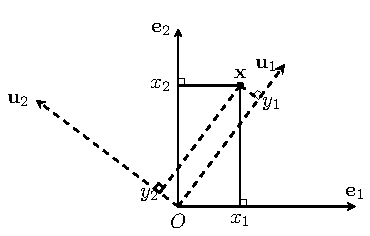
\includegraphics[width=.5\textwidth]{Chapters/07_DimemsionalityReduction/27_pca/latex/changebasis.pdf}
}
\end{figure}


Việc chuyển đổi hệ cơ sở sử dụng ma trận trực giao có thể được coi như một phép
xoay trục toạ độ. Nhìn theo một cách khác, đây cũng chính là một phép xoay
vector dữ liệu theo chiều ngược lại, nếu ta coi các trục toạ độ là cố định.
Trong Chương~\ref{cha:pca}, chúng ta sẽ thấy một ứng dụng quan trọng của
việc đổi hệ cơ sở.


% \newpage

\section{Trị riêng và vector riêng} % (fold)
\label{sec:tri_rieng_ve_vector_rieng}
\index{trị riêng -- eigenvalues}
\index{eigenvalues -- trị riêng}
\index{vector riêng -- eigenvectors}
\index{eigenvectors -- vector riêng}

\subsection{Định nghĩa} % (fold)
\label{sub:dinh_nghia}


% \def\C{\mathbb{C}}
Cho một ma trận vuông $\bA \in \mathbb{R}^{n\times n}$, một vector $\bx \in \mathbb{C}^n (\bx
\neq \mathbf{0} )$ và một số vô hướng $\lambda \in \mathbb{C}$. Nếu
% $\bA\bx = \lambda \bx$,
\begin{equation}
\bA\bx = \lambda \bx,
\end{equation}
ta nói $\lambda$ là một \textit{trị riêng} của $\bA$, $\bx$ là một \textit{vector riêng} ứng với trị riêng $\lambda$.
% và $\bx$ lần lượt là \textit{trị riêng, vector riêng} của ma trận $\bA$.

% thì ta nói rằng $\lambda$ và $\bx$ lần lượt
% là \textit{trị riêng} (\textit{eigenvalue}) và \textit{vector riêng}
% (\textit{eigenvector}) của ma trận $\bA$.


Từ định nghĩa ta cũng có $(\bA - \lambda \bI)\bx = 0$, tức $\bx$ là một vector nằm trong không gian $\mathcal{N}(\bA - \lambda \bI)$. Vì $\bx \neq 0$, ta có  $\bA - \lambda \bI$ là một ma
trận không khả nghịch. Nói cách khác $\det(\bA - \lambda \bI) = 0$, tức
$\lambda$ là nghiệm của phương trình $\det(\bA -t \bI) = 0$.
\index{da@đa thức đặc trưng -- characteristic polynomial}
\index{characteristic polynomial -- đa thức đặc trưng}
Định thức này là một đa thức bậc $n$ của $t$. Đa thức này còn được gọi là
\textit{đa thức đặc trưng} của $\bA$, được ký hiệu là $p_{\bA}(t)$. Tập hợp tất
\index{phổ của ma trận -- spectrum}
\index{spectrum -- phổ của ma trận}
cả các trị riêng của một ma trận vuông còn được gọi là \textit{phổ} của ma trận
đó.

% \subsection{Đa thức đặc trưng} % (fold)
% \label{sub:da_thuc_dac_trung}

% subsection da_thuc_dac_trung (end)

\subsection{Tính chất} % (fold)
\label{sub:tinh_chat}

% subsection tinh_chat (end)

% Định lý
% section trị_riêng_và_vector_riêng (end)



% \subsection{Trị riêng và vector riêng}
% Cho một ma trận vuông $\mathbf{A} \in \mathbb{R}^{n\times n}$, nếu số vô hướng
% $\lambda$ và vector $\mathbf{x} \neq \mathbf{0} \in \mathbb{R}^n$ thoả mãn:

% \begin{equation}
% \mathbf{Ax} = \lambda \mathbf{x}
% \end{equation}
% thì $\lambda$ được gọi là một trị riêng của $\mathbf{A}$ và $\mathbf{x}$ được gọi là vector riêng tương ứng với trị riêng đó.

% Một vài tính chất:

\def\ElA{E_{\lambda}(\bA)}
\begin{enumerate}
\item Giả sử $\lambda$ là một trị riêng của $\bA \in \mathbb{C}^{n\times n}$, đặt $\ElA$ là tập các vector riêng ứng với trị riêng $\lambda$ đó. Bạn đọc có thể chứng minh được:
\begin{itemize}
\item Nếu $\bx \in \ElA$ thì $k\bx \in \ElA, \forall k \in \mathbb{C}$.

\item Nếu $\bx_1, \bx_2 \in \ElA$ thì $\bx_1 + \bx_2 \in \ElA$.
\end{itemize}
Từ đó suy ra \textit{tập hợp các vector riêng ứng với một trị riêng của một
ma trận vuông tạo thành một không gian vector con}, thường được gọi là
\textit{không gian riêng} ứng với trị riêng đó.
\index{không gian riêng -- eigenspace}
\index{eigenspace -- không gian riêng}

\item \textit{Mọi ma trận vuông bậc $n$ đều có $n$ trị riêng, kể cả lặp và phức.}

\item \textit{Tích của tất cả các trị riêng của một ma trận bằng định thức
của ma trận đó. Tổng tất cả các trị riêng của một ma trận bằng tổng các
phần tử trên đường chéo của ma trận đó.}


\item \textit{Phổ của một ma trận bằng phổ của ma trận chuyển vị của nó.}


\item \textit{Nếu $\bA, \bB$ là các ma trận vuông cùng bậc thì
$p_{\bA\bB}(t) = p_ {\bB\bA}(t)$}. Như vậy, tuy $\bA\bB$ có thể khác
$\bB\bA$, đa thức đặc trưng của $\bA\bB$ và $\bB\bA$ luôn bằng nhau
nhau. Tức phổ của hai tích này là trùng nhau.

\item \textit{Tất cả các trị riêng của một ma trận Hermitian là các số
thực.} Thật vậy, giả sử $\lambda$ là một trị riêng của một ma trận Hermitian $\bA$ và $\bx$ là một vector riêng ứng với trị riêng đó. Từ định nghĩa ta
suy ra:
\begin{equation}
\bA\bx = \lambda\bx \Rightarrow (\bA\bx)^H = \bar{\lambda} \bx^H
\Rightarrow  \bar{\lambda}\bx^H = \bx^H\bA^H = \bx^H\bA
\end{equation}
với $\bar{\lambda}$ là liên hiệp phức của số vô hướng $\lambda$. Nhân cả hai
vế vào bên phải với $\bx$ ta có:
\begin{equation}
\bar{\lambda}\bx^H\bx = \bx^H\bA\bx = \lambda \bx^H \bx \Rightarrow
(\lambda - \bar{\lambda})\bx^H\bx = 0
\end{equation}
% Vì $\bx^H\bx$
vì $\bx \neq 0$ nên $\bx^H\bx \neq 0$. Từ đó suy ra $\bar{\lambda} =
\lambda$, tức $\lambda$ phải là một số thực.

\item Nếu $(\lambda, \bx)$ là một cặp trị riêng, vector riêng của một ma
trận khả nghịch $\bA$, thì $\displaystyle(\frac{1}{\lambda}, \bx)$ là một
cặp trị riêng, vector riêng của $\bA^{-1}$, vì $\displaystyle \bA\bx =
\lambda\bx \Rightarrow \frac{1} {\lambda}\bx = \bA^{-1}\bx$.


\end{enumerate}

%     \item Với \href{http://machinelearningcoban.com/2017/03/12/convexity/#positive-semidefinite}{\textit{ma trận xác định dương}}, tất cả
%     các trị riêng của nó đều là các số thực dương. Với \textit{ma trận nửa xác
%     định dương}, tất cả các trị riêng của nó đều là các số thực không âm.

% Tính chất cuối cùng có thể được suy ra từ định nghĩa của ma trận (nửa) xác định
% dương. Thật vậy, gọi $\mathbf{u} \neq \mathbf{0}$ là vector riêng ứng với một
% trị riêng $\lambda$ của ma trận $\mathbf{A}$ xác định dương, ta có:
% \begin{equation}
%     \mathbf{Au} = \lambda \mathbf{u} \Rightarrow \mathbf{u}^T\mathbf{Au} =
%                     \lambda \mathbf{u}^T\mathbf{u} = \lambda \|\mathbf{u}\|_2^2
% \end{equation}

% Vì $\mathbf{A}$ là nửa xác định dương nên với mọi $\mathbf{u} \neq \mathbf{0}$:
% $\mathbf{u}^T\mathbf{Au} \geq 0$; $\mathbf{u} \neq 0$ nên
% $\|\mathbf{u}\|_2^2 > 0$. Từ đó suy ra $\lambda$ là một số không âm.

\section{Chéo hoá ma trận} % (fold)
\label{sec:cheo_hoa_ma_tran}

Việc phân tích một đại lượng toán học ra thành các đại lượng nhỏ hơn mang lại
nhiều hiệu quả. Phân tích một số thành tích các thừa số nguyên tố giúp kiểm tra
một số có bao nhiêu ước số. Phân tích đa thức thành nhân tử giúp tìm nghiệm của
đa thức. Việc phân tích một ma trận thành tích của các ma trận đặc biệt cũng mang lại nhiều lợi ích trong việc giải hệ phương trình tuyến tính,
tính luỹ thừa của ma trận, xấp xỉ ma trận,... Trong mục này, chúng ta sẽ ôn
lại một phương pháp phân tích ma trận quen thuộc có tên là \textit{chéo hoá ma
trận}.

Giả sử $\bx_1, \dots, \bx_n \neq \mathbf{0}$ là các vector riêng của một ma trận
vuông $\bA$ ứng với các trị riêng lặp hoặc phức $\lambda_1, \dots, \lambda_n$:
\begin{math}
\bA\bx_i = \lambda_i \bx_i, ~\forall i = 1, \dots, n
\end{math}.

Đặt $\bLambda = \diag(\lambda_1, \lambda_2, \dots, \lambda_n)$, và
$\bX = \bmt \bx_1, \bx_2, \dots, \bx_n \emt$, ta sẽ có $\bA\bX = \bX\bLambda$.
Hơn nữa, nếu các trị riêng $\bx_1, \dots, \bx_n$ là độc lập tuyến tính, ma trận
$\bX$ là một ma trận khả nghịch. Khi đó ta có thể viết $\bA$ dưới dạng tích của
ba ma trận:
\begin{equation}
\label{eqn:eigendocomposition}
\bA = \bX\bLambda\bX^{-1}
\end{equation}
Các vector riêng $\bx_i$ thường được chọn sao cho $\bx_i^T\bx_i = 1$. Cách biểu
\index{phân tích trị riêng -- eigendecomposition}
\index{eigendecomposition -- phân tích trị riêng}
diễn một ma trận như~\eqref{eqn:eigendocomposition} được gọi là phép
\textit{phân tích trị riêng}.

\index{chéo hoá ma trận -- matrix diagonalization}
\index{matrix diagonalization -- chéo hoá ma trận}
Ma trận các trị riêng $\bLambda$ là một ma trận đường chéo. Vì vậy, cách khai
triển này cũng có tên gọi là \textit{chéo hoá ma trận}. Nếu ma trận $\bA$ có thể
phân tích được dưới dạng~\eqref{eqn:eigendocomposition}, ta nói rằng $\bA$ là
\textit{chéo hoá được}.

\subsection{Lưu ý} % (fold)
\label{sub:luu y}

% subsection luu y (end)Lưu ý
\begin{enumerate}

\item Khái niệm chéo hoá ma trận chỉ áp dụng với ma trận vuông. Vì không có
định nghĩa vector riêng hay trị riêng cho ma trận không vuông.

\item Không phải ma trận vuông nào cũng chéo hoá được. Một ma trận
vuông bậc $n$ chéo hoá được khi và chỉ khi nó có đủ $n$ vector riêng độc lập
tuyến tính.

\item Nếu một ma trận là chéo hoá được, có nhiều hơn một cách chéo hoá ma
trận đó. Chỉ cần đổi vị trí của các $\lambda_i$ và vị trí tương ứng
các cột của $\bX$, ta sẽ có một cách chéo hoá mới.

\item Nếu $\bA$ có thể viết được dưới dạng~\eqref{eqn:eigendocomposition},
khi đó các luỹ thừa có nó cũng chéo hoá được. Cụ thể:
\begin{equation}
\bA^2 = (\bX \bLambda \bX^{-1})(\bX \bLambda \bX^{-1}) =
\bX\bLambda^2\bX^{-1}; \quad \bA^k = \bX \bLambda^k \bX^{-1}, ~\forall k \in
\mathbb{N}
\end{equation}
Xin chú ý rằng nếu $\lambda$ và $\bx$ là một cặp trị riêng, vector riêng
của $\bA$, thì $\lambda^k$ và $\bx$ là một cặp  trị riêng, vector riêng
của $\bA^k$. Thật vậy, $\bA^k \bx = \bA^{k-1}(\bA\bx) = \lambda \bA^
{k-1}\bx = \dots = \lambda^k \bx$.

\item Nếu $\bA$ khả nghịch, thì $\bA^{-1} = (\bX \bLambda \bX^{-1})^{-1} =
\bX \bLambda^{-1}\bX^{-1}$.
\end{enumerate}

% section cheo_hoa_ma_tran (end)

\section{Ma trận xác định dương} % (fold)
\label{sec:ma_tran_xac_dinh_duong}
% \index{positive definite matrix}
% \index{positive definite matrix! positive semidefinite}
\index{xác định dương -- positive definite}
\index{positive definite -- xác định dương}
\index{nửa xác định dương -- positive semidefinite}
\index{positive semidefinite -- nửa xác định dương}
% Trong toán tối ưu, ma trận xác định dương đóng một vài trò rất quan trọng, đặc
% biệt là trong tối ưu lồi. Mục này chúng ta sẽ làm quen với định nghĩa và một
% vài tính chất của ma trận loại này.

\subsection{Định nghĩa} % (fold)
\label{sub:dinh_nghia}
Một ma trận đối xứng\footnote{Chú ý, tồn tại những ma trận không đối xứng thoả
mãn điều kiện~\eqref{eqn:semidefinite}. Ta sẽ không xét những ma trận này trong cuốn sách.}
% \index{xác định dương -- positive definite}
$\bA \in \R^{n\times n}$ được gọi là \textit{xác định dương} nếu:
\begin{equation}
\label{eqn:semidefinite}
\bx^T\bA\bx > 0, \forall \bx \in \R^{n}, \bx \neq \mathbf{0}.
\end{equation}
Một ma trận đối xứng $\bA \in \R^{n \times n}$ được gọi là \textit{nửa xác định
dương} nếu:
\begin{equation}
\bx^T\bA\bx \geq 0, \forall \bx \in \R^{n}, \bx \neq \mathbf{0}.
\end{equation}
Trên thực tế, ma trận nửa xác định dương được sử dụng nhiều hơn.

\index{nửa xác định âm -- negative semidefinite}
\index{negative semidefinite -- nửa xác định âm}
\index{xác định âm -- negative definite}
\index{negative definite -- xác định âm}

Ma trận \textit{xác định âm} và \textit{nửa xác định âm}  cũng được định nghĩa
tương tự.

Ký hiệu $\bA \succ 0, \succeq 0, \prec 0, \preceq 0$ lần lượt để chỉ một ma trận
là xác định dương, nửa xác định dương, xác định âm, và nửa xác định âm. Ký hiệu
$\bA \succ \bB$ cũng được dùng để chỉ ra rằng $\bA - \bB
\succ 0$.

Ví dụ, $\bA = \bmt 1 & -1 \\ -1 & 1\emt$ là nửa xác định dương vì với mọi vector
$\bx = \bmt u \\ v \emt$, ta có:
\begin{equation}
\bx^T \bA\bx = \bmt u & v \emt \bmt 1 & -1 \\ -1 & 1\emt \bmt u \\ v \emt =
u^2 + v^2 - 2uv = (u - v)^2 \geq 0, \forall u, v \in \R
\end{equation}

Mở rộng, một ma trận Hermitian $\bA \in \mathbb{C}^{n\times n}$ là xác định dương nếu
\begin{equation}
\bx^H\bA\bx > 0, \forall \bx \in \mathbb{C}^{n}, \bx \neq \mathbf{0}.
\end{equation}
Các khái niệm nửa xác định dương, xác định âm, và nửa xác định dương cũng được
định nghĩa tương tự cho các ma trận Hermitian.
\subsection{Tính chất} % (fold)
\label{sub:tinh_chat}
\begin{enumerate}

\item \textit{Mọi trị riêng của một ma trận Hermitian xác định dương đều là một số
thực dương.}  Trước hết, các trị riêng của một ma trận Hermitian là các số
thực. Để chứng minh chúng là các số thực dương, ta giả sử $\lambda$ là một
trị riêng của một ma trận xác định dương $\bA$ và $\bx \neq \mathbf{0}$ là
một vector riêng ứng với trị riêng đó. Nhân vào bên trái cả hai vế của
$\bA\bx = \lambda \bx$ với $\bx^H$ ta có:
\begin{equation}
\lambda \bx^H \bx = \bx^H \bA \bx > 0
\end{equation}
% (ở đây Hermitian được dùng để xét tổng quát cho cả trường hợp ma trận phức).
Vì $\forall \bx \neq \mathbf{0}, \bx^H\bx > 0$ nên ta phải có $\lambda > 0$. Tương
tự, ta có thể chứng minh được rằng mọi trị riêng của một ma trận
nửa xác định dương là không âm.


\item \textit{Mọi ma trận xác định dương đều khả nghịch. Hơn nữa, định thức
của nó là một số dương.}  Điều này được trực tiếp suy ra từ tính chất (a).
Nhắc lại rằng định thức của một ma trận bằng tích tất cả các trị riêng của
nó.

\index{ma trận con chính -- principal submatrix}
\index{principal submatrix -- ma trận con chính}
\index{ma trận con chính trước -- leading principal submatrix}
\index{leading principal submatrix -- ma trận con chính trước}

\def\AI{\bA_{\mathcal{I}}}
\item Tiêu chuẩn Sylvester. Trước hết, chúng ta làm quen với hai khái niệm:
\textit{ma trận con chính} và \textit{ma trận con chính trước}.

Giả sử $\bA$ là một ma trận vuông bậc $n$. Gọi $\mathcal{I}$ là một tập con
khác rỗng bất kỳ của $\{1, 2, \dots, n\}$, ký hiệu $\AI$ để chỉ một ma trận
con của $\bA$ nhận được bằng cách trích ra các hàng và cột có chỉ số nằm
trong $\mathcal{I}$ của $\bA$. Khi đó, $\AI$ được gọi là một \textit{ma trận
con chính} của $\bA$. Nếu $\mathcal{I}$ chỉ bao gồm các số tự nhiên liên
tiếp từ $1$ đến $k \leq  n$, ta nói $\AI$ là một \textit{ma trận con chính
trước} bậc $k$ của $\bA$.

Tiêu chuẩn Sylvester nói rằng: \textit{Một ma trận Hermitian là xác định dương khi và chỉ khi mọi \textbf{ma trận con chính trước} của nó là xác định dương}.

Các ma trận Hermitian nửa xác định dương cần điều kiện chặt hơn: \textit{Một
ma trận Hermitian là nửa xác định dương khi và chỉ khi mọi \textbf{ma trận
con chính} của nó là nửa xác định dương}.


% \item Tiêu chuẩn Sylvester: \textit{Một ma trận Hermitian là xác định dương
% khi và chỉ khi mọi \textit{ma trận con chính trước} của nó là dương. Một ma trận
% Hermitian là nửa xác định dương nếu mọi principal minors của nó là không
% âm}. Đây là một tiêu chuẩn để kiểm tra một ma trận Hermitian $\bA \in \R^n$
% có là (nửa) xác định dương hay không. Ở đây, \textit{leading principal
% minors} và \textit{principal minors} được định nghĩa như sau:

% \index{submatrix!principal submatrix}
% \index{submatrix!principal minor}
% \index{submatrix!leading principal minor}
% \index{submatrix!leading principal matrix}

% Gọi $\mathcal{I}$ là một tập con bất kỳ của $\{1, 2, \dots, n\}$, $\AI$ là ma
% trận con của $\bA$ nhận được bằng cách trích ra các hàng và cột có chỉ số
% nằm trong $\mathcal{I}$ của $\bA$. Khi đó, $\AI$ và $\det(\AI)$ lần lượt
% được gọi là một \textit{ma trận con chính} (\textit{principal submatrix}) và
% \textit{principal minor} của $\bA$. Nếu $\mathcal{I}$ chỉ
% bao gồm các số tự nhiên liên tiếp từ $1$ đến $k \leq  n$, ta nói $\AI$ và
% $\det(\AI)$ lần lượt là một \textit{leading principal submatrix} và
% \textit{leading principal minor} bậc $k$ của $\bA$.

\item \textit{Với mọi ma trận $\bB$ không nhất thiết vuông, ma trận $\bA = \bB^H\bB$ là nửa xác định dương}.
% \textit{$\bA = \bB^H\bB$ là nửa xác định dương với mọi ma trận $\bB$
% (không nhất thiết vuông).}
Thật vậy, với mọi vector $\bx \neq 0$ với chiều phù hợp, $\bx^H\bA\bx =
\bx^H\bB^H\bB\bx = (\bB\bx)^H(\bB\bx) \geq 0$.
\index{Phân tích Cholesky -- Cholesky decomposition}
\index{Cholesky decomposition -- Phân tích Cholesky}
\item Phân tích Cholesky: \textit{Mọi ma trận Hermitian nửa xác định dương
$\bA$ đều biểu diễn được duy nhất dưới dạng $\bA = \bL\bL^H$ với $\bL$ là
một ma trận tam giác dưới với các thành phần trên đường chéo là thực dương}.

\item \textit{Nếu $\bA$ là một ma trận nửa xác định dương thì
$\bx^T\bA\bx = 0 \Leftrightarrow \bA\bx = 0$.}

Nếu $\bA\bx = 0$, dễ thấy $\bx^T\bA\bx = 0$. Nếu $\bx^T\bA\bx = 0$, với $\by \neq \mathbf{0}$ bất kỳ có cùng kích thước với $\bx$, xét hàm số
\begin{equation}
f(\lambda) = (\bx + \lambda \by)^T\bA(\bx + \lambda\by)
\end{equation}
Hàm số này không âm với mọi $\lambda$ vì $\bA$ là một ma trận nửa xác định
dương. Đây là một tam thức bậc hai của $\lambda$:
\begin{equation}
f(\lambda) = \by^T\bA\by \lambda^2 + 2\by^T\bA\bx \lambda + \bx^T\bA\bx
= \by^T\bA\by \lambda^2 + 2\by^T\bA\bx \lambda
\end{equation}
Xét hai trường hợp:
\begin{itemize}

\item $\by^T\bA\by = 0$. Khi đó, $f(\lambda) = 2\by^T\bA\bx \lambda
\geq 0, \forall \lambda$ khi và chỉ khi $\by^T\bA\bx = 0$.

\item $\by^T\bA\by > 0$. Khi đó tam thức bậc hai $f(\lambda) \geq 0,
\forall \lambda$ xảy ra khi và chỉ khi $\Delta' = (\by^T\bA\bx)^2 \leq
0$. Điều này cũng đồng nghĩa với việc $\by^T\bA\bx = 0$
\end{itemize}
Tóm lại, $\by^T\bA\bx = 0, ~\forall \by \neq \mathbf{0}$. Điều này chỉ xảy
ra nếu $\bA\bx = 0$.  \dpcm %\hfill $\square$

\end{enumerate}
% subsection tinh_chat (end)




% Nếu dấu bằng xảy ra tại một vài $\bx \neq \mathbf{0}$, ta

% subsection dinh_nghia (end)

% \begin{mydef}{Ma trận xác định dương}
% f
% \end{mydef}

% section ma_tran_xac_dinh_duong (end)

\index{chuẩn -- norm}
\index{norm -- chuẩn}
\section{Chuẩn}
\label{sec:2_norm}
Trong không gian một chiều, khoảng cách giữa hai điểm là trị tuyệt đối của hiệu
giữa hai giá trị đó. Trong không gian hai chiều, tức mặt phẳng, chúng ta thường
dùng khoảng cách Euclid để đo khoảng cách giữa hai điểm. Khoảng cách Euclid
chính là độ dài đoạn thẳng nối hai điểm trong mặt phẳng. Đôi khi, để đi từ một
điểm này tới một điểm kia, chúng ta không thể đi bằng đường thẳng vì còn phụ
thuộc vào hình dạng đường đi nối giữa hai điểm.

Việc đo khoảng cách giữa hai điểm dữ liệu nhiều chiều rất cần thiết trong
machine learning. Đây chính là lý do khái niệm \textit{chuẩn} ({norm}) ra
đời. Để xác định khoảng cách giữa hai vector $\mathbf{y}$ và $\mathbf{z}$, người
ta thường áp dụng một hàm số lên vector hiệu $\mathbf{x = y - z}$. Hàm số này
cần có một vài tính chất đặc biệt.

% \subsection{Định nghĩa}
\begin{mydef}{Chuẩn -- Norm}
Một hàm số $f: \R^n \rightarrow \R$ được gọi là một chuẩn nếu nó thỏa mãn ba
điều kiện sau đây:
\begin{enumerate}

\item $f(\mathbf{x}) \geq 0$. Dấu bằng xảy ra $\Leftrightarrow \mathbf{x = 0} $.

\item $f(\alpha \mathbf{x}) = |\alpha| f(\mathbf{x}), ~~~\forall \alpha \in \mathbb{R}\ $

\item $f(\mathbf{x}_1) + f(\mathbf{x}_2) \geq f(\mathbf{x}_1 + \mathbf{x}_2),
~~\forall \mathbf{x}_1, \mathbf{x}_2 \in \mathbb{R}^n$

\end{enumerate}\end{mydef}

{Điều kiện a)} là dễ hiểu vì khoảng cách không thể là một số âm.
Hơn nữa, khoảng cách giữa hai điểm $\mathbf{y}$ và $\mathbf{z}$ bằng 0 khi và
chỉ khi hai điểm đó trùng nhau, tức $\mathbf{x = y - z = 0} $.

{Điều kiện b)} cũng có thể được lý giải như sau. Nếu ba điểm
$\mathbf{y, v}$ và $\mathbf{z}$ thẳng hàng, hơn nữa
$\mathbf{v - y} = \alpha (\mathbf{v - z}) $ thì khoảng cách giữa $\mathbf{v}$ và
$\mathbf{y}$ gấp $ |\alpha |$ lần khoảng cách giữa $\mathbf{v}$ và
$\mathbf{z}$.

{Điều kiện c)} chính là bất đẳng thức tam giác nếu ta coi
$\mathbf{x}_1 = \mathbf{y - w}, \mathbf{x}_2 = \mathbf{w - z} $ với
$\mathbf{w}$ là một điểm bất kỳ trong cùng không gian.



\subsection{Một số chuẩn vector thường dùng}
\label{sub:norms}
% Giả sử các vectors $\mathbf{x} = [x_1; x_2; \dots; x_n]$,
% $\mathbf{y} = [y_1; y_2; \dots; y_$.

\index{chuẩn -- norm!chuẩn $\ell_2$ -- $\ell_2$ norm}
\index{norm -- chuẩn!$\ell_2$ norm -- chuẩn $\ell_2$}
\index{chuẩn -- norm!chuẩn Euclid -- Euclidean norm}
\index{norm -- chuẩn!Euclidean norm -- chuẩn Euclid}

Độ dài Euclid của một vector $\bx \in \R^n$ chính là một chuẩn, chuẩn này
được gọi là chuẩn $\ell_2$ hoặc chuẩn Euclid:
\begin{equation}
\label{eqn:norm2}
\|\mathbf{x}\|_2 = \sqrt{x_1^2 + x_2^2 + \dots + x_n^2}
\end{equation}
Bình phương của chuẩn $\ell_2$ chính là tích vô hướng của một vector với chính nó,
$\|\mathbf{x}\|_2^2 = \bx^T\bx$.
\index{chuẩn -- norm!chuẩn $\ell_p$}
\index{norm -- chuẩn!chuẩn $\ell_p$}

\newpage Với $p$ {là một số không nhỏ hơn 1} bất kỳ, hàm số:
\begin{equation}
\label{eqn:normp}
\|\mathbf{x}\|_p = (|x_1|^p + |x_2|^p + \dots |x_n|^p)^{\frac{1}{p}}
\end{equation}
được chứng minh thỏa mãn ba điều kiện của chuẩn, và được gọi là {chuẩn $\ell_p$}.
    

% Nhận thấy rằng khi $p \rightarrow 0 $ thì biểu thức \eqref{eqn:normp} trở thành
% \textit{số các phần tử khác 0 của} $\mathbf{x}$. Hàm số \eqref{eqn:normp} khi
% $p = 0$ được gọi là giả chuẩn (pseudo-norm) 0. Nó không phải là norm vì nó không
% thỏa mãn điều kiện 2 và 3 của norm. Giả chuẩn này, thường được ký hiệu là
% $\|\mathbf{x}\|_0$, chính là số lượng thành phần khác không của $\mathbf{x}$.
% Giả chuẩn này khá quan trọng trong Machine Learning vì trong nhiều bài toán,
% chúng ta cần có ràng buộc “sparse”, tức số lượng thành phần khác không của
% $\mathbf{x}$ là nhỏ.


% ******************************************************************************
\begin{figure}[t]
% caption on side
\floatbox[{\capbeside\thisfloatsetup{capbesideposition={right,top},
capbesidewidth=6.5cm}}]{figure}[\FBwidth]
{%\caption{
\caption{Minh họa chuẩn $\ell_1$ và chuẩn $\ell_2$ trong không gian hai chiều.
Chuẩn $\ell_2$ chính
là khoảng cách Euclid. Trong khi đó chuẩn $\ell_1$ là quãng
đường ngắn nhất giữa hai điểm nếu chỉ được đi theo các đường song song với
các trục toạ độ.}
\label{fig:norm12}}
{ % figure here
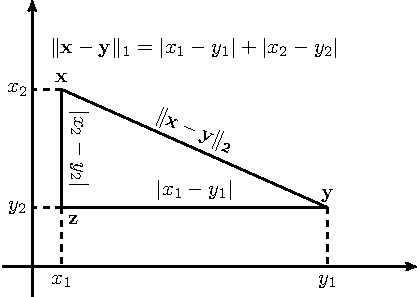
\includegraphics[width=.5\textwidth]{Chapters/02_LinearAlgebra/linearalgebra/norm12.pdf}
}
\end{figure}
% ******************************************************************************
Dưới đây là một vài giá trị của $p$ thường được dùng.
\begin{enumerate}
\item Khi $p = 2$, ta có chuẩn $\ell_2$ như ở trên.

\index{chuẩn -- norm!chuẩn $\ell_1$}
\index{norm -- chuẩn!chuẩn $\ell_1$}
\item Khi $p = 1$, ta có chuẩn $\ell_1$:
$\|\mathbf{x}\|_1 = |x_1| + |x_2| + \dots +|x_n|$ là tổng các trị tuyệt đối
của từng phần tử của $\mathbf{x}$. Hình \ref{fig:norm12} là một ví dụ  sánh
chuẩn $\ell_1$ và chuẩn $\ell_2$ trong không gian hai chiều. Chuẩn $\ell_2$
chính là khoảng cách Euclid giữa $\mathbf{x} $ và
$\mathbf{y}$. Trong khi đó, khoảng cách chuẩn $\ell_1$ giữa hai điểm này
(đường gấp khúc $\bx\bz\by$) có thể diễn giải như là quãng đường từ $\mathbf{x}
$ tới $\mathbf{y}$ nếu chỉ được phép đi song song với các trục toạ độ.

\item Khi $p \rightarrow \infty $, giả sử
$i = \arg\max_{j=1, 2, \dots, n} |x_j|$. Khi đó:
\begin{equation}
\|\bx\|_p = |x_i|\left(1 + \left|\frac{x_1}{x_i}\right|^p +
\dots +
\left|\frac{x_{i-1}}{x_i}\right|^p + \left|\frac{x_{i+1}}{x_i}\right|^p
+ \dots +\left|\frac{x_{n}}{x_i}\right|^p\right)^{\frac{1}
{p}}
\end{equation}
Ta thấy rằng
\begin{equation}
\lim_{p \rightarrow \infty}\left(1 + \left|\frac{x_1}{x_i}\right|^p +
\dots +
\left|\frac{x_{i-1}}{x_i}\right|^p + \left|\frac{x_{i+1}}{x_i}\right|^p
+ \dots +\left|\frac{x_{n}}{x_i}\right|^p\right)^{\frac{1}{p}} = 1
\end{equation}
vì đại lượng trong dấu ngoặc đơn không vượt quá $n$. Ta có
\begin{equation}
\|\bx\|_{\infty} \triangleq \lim_{p \rightarrow \infty} \|\bx\|_{p} =
|x_i| = \max_{j=1, 2, \dots, n} | x_j|
\end{equation}

\end{enumerate}

\subsection{Chuẩn Frobenius của ma trận}
\index{chuẩn -- norm!chuẩn Frobenius -- Frobenius norm}
\index{norm -- chuẩn!Frobenius norm -- chuẩn Frobenius}
Với một ma trận $\mathbf{A} \in \mathbb{R}^{m\times n}$, chuẩn thường được dùng
nhất là chuẩn Frobenius, ký hiệu là $\|\mathbf{A}\|_F$, là căn bậc hai của tổng
bình phương tất cả các phần tử của nó:
\begin{equation*}
\|\mathbf{A}\|_F = \sqrt{\sum_{i = 1}^m \sum_{j = 1}^n a_{ij}^2}
\end{equation*}
Chú ý rằng chuẩn $\ell_2$, $\|\bA\|_2$, là một chuẩn khác của ma trận, không phổ biến bằng
chuẩn Frobenius. Bạn đọc có thể xem chuẩn $\ell_2$ của ma trận trong Phụ lục~\ref{apd:lagrange}.
% \subsection{Norm 2 của ma trận}

% Chúng ta vẫn thường nhắc nhiều đến  \href{http://machinelearningcoban.com/math
% /#-norms-chuan}{norm cho vector}  nhưng chưa thực sự làm việc nhiều với norm của
% ma trận (ngoài  \href{http://machinelearningcoban.com/math/#chuan-cua-ma-
% tran}{Frobenius norm}). Trong mục này, chúng ta sẽ làm quen với 1 lớp các norm
% cho ma trận được định nghĩa dựa trên norm của vector. Lớp các norms này còn được
% gọi là \textit{Induced Norms}.

% Giả sử hàm số $\|\mathbf{x}\|_{\alpha}$ là một norm bất kỳ của vector
% $\mathbf{x}$. Ứng với norm này, định nghĩa norm tương ứng cho ma trận
% $\mathbf{A}$:
% \begin{equation}
% \|\mathbf{A}\|_{\alpha} = \max_{\mathbf{x}} \frac{\|\mathbf{Ax}\|_{\alpha}}{\|\mathbf{x}\|_{\alpha}}
% \end{equation}

% chú ý rằng ma trận $\mathbf{A}$ có thể không vuông và số cột của nó bằng với số
% chiều của $\mathbf{x}$. Như vậy, bản thân việc tính toán norm của ma trận là
% việc giải một bài toán tối ưu. Chú ý rằng hàm tối ưu có cả tử số và mẫu số là
% các norm trên vectors.

% Chúng ta sẽ quan m nhiều hơn tới chuẩn $\ell_2$. Norm 2 của ma trận được định nghĩa là:
% \begin{equation}
% \label{eqn:27_1}
% \|\mathbf{A}\|_2 = \max_{\mathbf{x}} \frac{\|\mathbf{Ax}\|_2}{\|\mathbf{x}\|_2}
% \end{equation}

% Nhận thấy rằng nếu $\mathbf{x}$ là nghiệm của bài toán tối ưu \eqref{eqn:27_1}
% thì $k\mathbf{x}$ cũng là nghiệm với $k$ là một số thực khác không bất kỳ. Không
% mất tính tổng quát, ta có thể giả sử mẫu số bằng 1. Khi đó, bài toán tối ưu
% \eqref{eqn:27_1} có thể được viết dưới dạng:
% \begin{equation}
%     \label{eqn:27_2}
%     \|\mathbf{A}\|_2 = \max_{\|\mathbf{x}\|_2 = 1} \|\mathbf{Ax}\|_2
% \end{equation}
% Nói cách khác, ta cần đi tìm $\mathbf{x}$ sao cho:
% \begin{equation}
% \label{eqn:27_3}
% \begin{aligned}
% \mathbf{x} &= \text{argmax}_{\mathbf{x}} \|\mathbf{Ax}\|_2^2  \\\
% \text{s.t.: } & \|\mathbf{x}\|_2^2 = 1
% \end{aligned}
% \end{equatn}
% Ở đây, các chuẩn $\ell_2$ đã được bình phương lên để tránh dấu căn bậc hai. Bài toán
% \eqref{eqn:27_3} có thể được giải bằng
% \href{http://machinelearningcoban.com/2017/04/02/duality/# -- phuong-phap-nhan-tu-lagrange}{Phương pháp nhân tử Lagrange}
% vì ràng buộc là một phương trình.

% Lagrangian của Bài toán \eqref{eqn:27_3} là:
% \begin{equation}
% \mathcal{L}(\mathbf{x}, \lambda) = \|\mathbf{Ax}\|_2^2 + \lambda (1 - \|\mathbf{x}\|_2^2)
% \end{equation}

% Nghiệm của bài toán \eqref{eqn:27_3} sẽ thoả mãn hệ phương trình:
% \begin{eqnarray}
%     \label{eqn:27_4}
%     \frac{\partial \mathcal{L}}{\partial \mathbf{x}} &=& 2\mathbf{A}^T\mathbf{Ax} - 2\lambda \mathbf{x} = \mathbf{0} \\\
%     \label{eqn:27_5}
%     \frac{\partial \mathcal{L}}{\partial \lambda} &=& 1 - \|\mathbf{x}\|_2^2 = 0
% \end{eqnarray}

% Từ \eqref{eqn:27_4} ta có:
% \begin{equation}
%     \label{eqn:27_6}
%     \mathbf{A}^T\mathbf{Ax} = \lambda\mathbf{x}
% \end{equation}
% Điều này suy ra rằng $\lambda$ là một trị riêng của $\mathbf{A}^T\mathbf{A}$ và $\mathbf{x}$ là 1 vector riêng ứng với trị riêng đó. Tiếp tục nhân hai vế của \eqref{eqn:27_6} với $\mathbf{x}^T$ vào bên trái, ta có:
% \begin{equation}
% \mathbf{x}^T\mathbf{A}^T\mathbf{Ax} = \lambda \mathbf{x}^T\mathbf{x} = \lambda
% \end{equation}
% Nhận thấy rằng vế trái chính là $\|\mathbf{Ax}\|_2^2$ chính là hàm mục tiêu
% trong \eqref{eqn:27_3}. Vậy hàm mục tiêu đạt giá trị lớn nhất khi $\lambda$
% đạt giá trị lớn nhất. Nói cách khác, $\lambda$ chính là trị riêng lớn nhất của
% $\mathbf{A}^T\mathbf{A}$ hay chính là \href{http://machinelearningcoban.com/2017/06/07/svd/#-nguon-goc-ten-goi-singular-value-decomposition}{singular value} lớn
% nhất của ma trận $\mathbf}$.

% Như vậy, chuẩn $\ell_2$ của một ma trận chính là singular value lớn nhất của ma trận đó.
% Và nghiệm của bài toán \eqref{eqn:27_3} chính một là \textit{right-singular
% vector} ứng với singular value đó.

% Với lý luận tương tự, chúng ta có thể suy ra rằng bài toán:
% \begin{equation}
%     \min_{\|\mathbf{x}\|_2 =1} \mathbf{x}^T\mathbf{A}^T\mathbf{A}\mathbf{x}
% \end{equation}

% có nghiệm là vector riêng ứng với trị riêng nhỏ nhất của
% $\mathbf{A}^T\mathbf{A}$. Khi đó, hàm số đạt giá trị nhỏ nhất bằng chính trị
% riêng nhỏ nhất này.


\section{Vết}
\index{vết -- trace}
\index{trace -- vết}
\textit{Vết} (trace) của một ma trận vuông $\bA$ được ký hiệu là $\trace(\bA)$, là tổng
tất cả các phần tử trên đường chéo chính của nó. Hàm vết xác định trên tập các
ma trận vuông được sử dụng nhiều trong tối ưu vì nó có những tính chất đẹp.

Các tính chất quan trọng của hàm vết, với giả sử rằng các ma trận trong hàm
vết là vuông và các phép nhân ma trận thực hiện được:
\begin{enumerate}
\item \textit{Một ma trận vuông bất kỳ và chuyển vị của nó có vết bằng
nhau}: $\trace(\bA) = \trace(\bA^T)$. Việc này được suy ra từ việc phép
chuyển vị không làm thay đổi các phần tử trên đường chéo chính của một ma
trận.


\item \textit{Vết của một tổng bằng tổng các vết}:
$$\displaystyle\trace(\sum_{i=1}^k \bA_i) = \sum_{i=1}^k \trace(\bA_i)$$

\item $\trace(k\mathbf{A}) = k\trace(\mathbf{A})$ với $k$ là một
số vô hướng bất kỳ.

\item $\trace(\mathbf{A}) = \sum_{i = 1}^D \lambda_i $ với
$\mathbf{A}$ là một ma trận vuông và $\lambda_i, i = 1, 2, \dots, N$ là toàn
bộ các trị riêng của nó, có thể lặp hoặc phức. Việc chứng minh tính chất này
có thể được dựa trên ma trận đặc trưng của $\mathbf{A}$ và định lý Viète.

\item $\trace(\mathbf{AB}) = \trace(\mathbf{BA})$. Đẳng thức này
được suy ra từ việc đa thức đặc trưng của $\bA\bB$ và $\bB\bA$ là như nhau.
Bạn đọc cũng có thể chứng minh bằng cách tính trực tiếp các phần tử trên
đường chéo chính của $\bA\bB$ và $\bB\bA$.

\item $\trace(\bA\bB\bC) = \trace(\bB\bC\bA)$, nhưng $\trace(\bA\bB\bC)$
không đồng nhất với $\trace(\bA\bC\bB)$.

\item Nếu $\bX$ là một ma trận khả nghịch cùng chiều với $\bA$ thì
\begin{equation*}
\trace (\bX\bA\bX^{-1}) = \trace(\bX^{-1}\bX\bA) = \trace(\bA)
\end{equation*}
\item $\|\mathbf{A}\|_F^2 = \trace(\mathbf{A}^T\mathbf{A}) =
\trace(\mathbf{A}\mathbf{A}^T)$ với $\mathbf{A}$ là một ma trận bất kỳ. Từ
đây ta cũng suy ra $\trace(\bA\bA^T) \geq 0$ với mọi ma trận $\bA$.

\end{enumerate}

% !TEX root = ../../book_ML.tex

\chapter{Giải tích ma trận}

% for increase vertical distance in matrix
\def\largevspace{\renewcommand{\arraystretch}{2}}
\def\smallvspace{\renewcommand{\arraystretch}{1}}

% \index{giải tcismatrix calculus}
% \section{Đạo hàm của hàm nhiều biến }
% \textit{Trong chương này, chúng ta sẽ giả sử rằng các đạo hàm tồn tại. Chúng ta sẽ xét hai trường hợp: i) Hàm số nhận giá trị là ma trận (vector) và cho giá trị là một số thực vô hướng; và ii) Hàm số nhận giá trị là một số vô hướng hoặc vector và cho giá trị là một vector.
% }
\vspace{-1.2in}
Giả sử rằng các gradient tồn tại trong toàn bộ chương. Tài liệu tham khảo
chính của chương là \textit{Matrix calculus -- Stanford}
(\url{https://goo.gl/BjTPLr}).

\largevspace
\section{Gradient của hàm trả về một số vô hướng}
\index{gradient}
\index{gradient!gradient bậc nhất -- first-order gradient}
\index{gradient!first-order gradient -- gradient bậc nhất}
\index{partial derivative -- đạo hàm riêng}
\index{đạo hàm riêng -- partial derivative}
\textit{Gradient bậc nhất} ({first-order gradient}) hay viết gọn là
{gradient} của một hàm số $f(\bx): \mathbb{R}^n
\rightarrow
\mathbb{R}$
theo $\bx$, ký hiệu là $\nabla_{\bx} f(\bx)$, được định nghĩa bởi
\begin{equation}
\label{eqn:grvector1}
\nabla_{\bx} f(\bx) \triangleq
\left[
\begin{matrix}
\dfrac{\partial f(\bx)}{\partial x_1} \\\
\dfrac{\partial f(\bx)}{\partial x_2} \\\
\vdots \\\
\dfrac{\partial f(\bx)}{\partial x_n}
\end{matrix}
\right] \in \mathbb{R}^n,
\end{equation}
trong đó $\displaystyle\dfrac{\partial f(\bx)}{\partial x_i}$ là \textit{đạo hàm
riêng} của hàm số theo thành phần thứ $i$ của
vector $\bx$. Đạo hàm này được tính khi tất cả các biến, ngoài $x_i$, được giả sử
là hằng số. Nếu không có thêm biến nào khác, $\nabla_{\bx}f(\bx)$ thường được
viết gọn là $\nabla f(\bx)$. {Gradient của hàm số này là một vector có
cùng chiều với vector đang được lấy gradient}. Tức nếu vector được viết ở dạng
cột thì gradient cũng phải được viết ở dạng cột.% Ta cần tính đạo hàm riêng theo từng thành phần của vector rồi sắp xếp chúng lại theo đúng thứ tự ban đầu.

\index{gradient!gradient bậc hai -- second-order gradient}
\index{gradient!second-order gradient -- gradient bậc hai}
\index{Hesse -- Hessian}
\index{Hessian -- Hesse}
\textit{Gradient bậc hai} ({second-order gradient}) của hàm số trên còn
được gọi là \textit{Hesse} (Hessian) và được định nghĩa như sau:

\begin{equation}
\label{eqn:hessian1}
\nabla^2 f(\bx) \triangleq
\bmt
\dfrac{\partial^2 f(\bx)}{\partial x_1^2} & \dfrac{\partial^2 f(\bx)}{\partial x_1\partial x_2} & \dots & \dfrac{\partial^2 f(\bx)}{\partial x_1\partial x_n} \\\
\dfrac{\partial^2 f(\bx)}{\partial x_2\partial x_1} & \dfrac{\partial^2 f(\bx)}{\partial x_2^2} & \dots & \dfrac{\partial^2 f(\bx)}{\partial x_2\partial x_n} \\\
\vdots & \vdots & \ddots & \vdots \\\
\dfrac{\partial^2 f(\bx)}{\partial x_n\partial x_1} & \dfrac{\partial^2 f(\bx)}{\partial x_n\partial x_2} & \dots & \dfrac{\partial^2 f(\bx)}{\partial x_n^2}
\emt \in \mathbb{S}^{n}.
\end{equation}


Gradient của một hàm số $f(\bX): \mathbb{R}^{n \times m} \rightarrow
\mathbb{R}$ {theo ma trận} $\bX$ được định nghĩa là
\begin{equation}
\label{eqn:grmatrix1}
\nabla f(\bX) =
\bmt
\dfrac{\partial f(\bX)}{\partial x_{11}} & \dfrac{\partial f(\bX)}{\partial x_{12}} & \dots & \dfrac{\partial f(\bX)}{\partial x_{1m}} \\\
\dfrac{\partial f(\bX)}{\partial x_{21}} & \dfrac{\partial f(\bX)}{\partial x_{22}} & \dots & \dfrac{\partial f(\bX)}{\partial x_{2m}} \\\
\vdots & \vdots & \ddots & \vdots \\\
\dfrac{\partial f(\bX)}{\partial x_{n1}} & \dfrac{\partial f(\bX)}{\partial x_{n2}} & \dots & \dfrac{\partial f(\bX)}{\partial x_{nm}}
\emt \in \mathbb{R}^{n \times m}.
\end{equation}
\newnote{}{
Gradient của hàm số $f: \R^{m\times n} \rightarrow \R$ là một ma trận trong
$\R^{m\times n}.$
}
Cụ thể, để tính gradient của một hàm $f: \R^{m\times n} \rightarrow \R$, ta tính
đạo hàm riêng của hàm số đó theo từng thành
phần của ma trận {khi toàn bộ các thành phần khác được giả sử là hằng
số}. Tiếp theo, ta sắp xếp các đạo hàm riêng tính được theo đúng thứ tự
trong ma trận.

{\textit{Ví dụ}}: Xét hàm số $f: \mathbb{R}^2 \rightarrow \mathbb{R}$, $f(\bx) =
x_1 ^2 + 2x_1x_2 + \sin(x_1) + 2$. Gradient bậc nhất theo $\bx$ của hàm số đó là
\begin{equation*}
\nabla f(\bx) =
\bmt
\dfrac{\partial f(\bx)}{\partial x_1} \\\
\dfrac{\partial f(\bx)}{\partial x_2}
\emt = \bmt
2x_1 + 2x_2 + \cos(x_1) \\\
2x_1
\emt.
\end{equation*}

Gradient bậc hai theo $\bx$, hay Hesse là
% \begin{equation*}
$$
\nabla^2 f(\bx) =
\bmt
\dfrac{\partial^2 f(\bx)}{\partial x_1^2} & \dfrac{\partial f^2(\bx)}{\partial x_1\partial x_2} \\\
\dfrac{\partial^2 f(\bx)}{\partial x_2\partial x_1} & \dfrac{\partial f^2(\bx)}{\partial x_2^2}
\emt =
\bmt
2 - \sin(x_1) & 2 \\\
2 & 0
\emt.$$
% \end{equation*}
Chú ý rằng {Hesse} luôn là một ma trận đối xứng.


\section{Gradient của hàm trả về vector }

\index{hàm trả về vector -- vector-valued function}
\index{vector-valued function -- hàm trả về vector}
Những hàm số mà đầu ra là một vector được gọi là \textit{hàm trả về vector} (vector-valued function).

Xét một hàm trả về vector với đầu vào là một số thực $v(x):
\mathbb{R} \rightarrow
\mathbb{R}^n $:
\smallvspace
\begin{equation}
\label{eqn:vectorvalued}
v(x) =
\bmt
v_1(x) \\\
v_2(x) \\\
\vdots \\\
v_n(x)
\emt.
\end{equation}
Gradient của hàm số này theo $x$ là một {vector hàng} như sau:
\begin{equation}
\label{eqn:grvectorvalued}
\nabla v(x) \triangleq
\bmt
\dfrac{\partial v_1(x)}{\partial x} & \dfrac{\partial v_2(x)}{\partial x} &
\dots & \dfrac{\partial v_n(x)}{\partial x}
\emt.
\end{equation}
Gradient bậc hai của hàm số này có dạng:
\begin{equation}
\label{eqn:hessianvectorvalued}
\nabla^2 v(x) \triangleq
\left[
\begin{matrix}
\dfrac{\partial^2 v_1(x)}{\partial x^2} & \dfrac{\partial^2 v_2(x)}{\partial x^2} & \dots & \dfrac{\partial^2 v_n(x)}{\partial x^2}
\end{matrix}
\right].
\end{equation}

\vd Cho một vector $\mathbf{a} \in \mathbb{R}^n$ và một hàm số trả về
vector $v(x) = x\mathbf{a}$, gradient và Hesse của nó lần lượt là
\begin{equation}
\nabla v(x) = \mathbf{a}^T, ~~~ \nabla^2 v(x) = \mathbf{0} \in \mathbb{R}^{1\times n}.
\end{equation}
Xét một hàm trả về vector với {đầu vào là một vector}
$h(\bx):\mathbb{R}^k \rightarrow \mathbb{R}^n$, gradient của nó là
\begin{eqnarray}
\label{eqn:gdvectorvector}
\nabla h(\bx) &\triangleq &
\bmt
\dfrac{\partial h_1(\bx)}{\partial x_1} & \dfrac{\partial h_2(\bx)}{\partial x_1} & \dots & \dfrac{\partial h_n(\bx)}{\partial x_1} \\\
\dfrac{\partial h_1(\bx)}{\partial x_2} & \dfrac{\partial h_2(\bx)}{\partial x_2} & \dots & \dfrac{\partial h_n(\bx)}{\partial x_2} \\\
\vdots & \vdots & \ddots & \vdots \\\
\dfrac{\partial h_1(\bx)}{\partial x_k} & \dfrac{\partial h_2(\bx)}{\partial x_k} & \dots & \dfrac{\partial h_n(\bx)}{\partial x_k}
\emt =
\bmt
\nabla h_1(\bx) & \dots & \nabla h_n(\bx)
\emt \in \mathbb{R}^{k\times n}.
\end{eqnarray}

\newnote{}{
Gradient của hàm số $g: \mathbb{R}^m \rightarrow \mathbb{R}^n$ là
một ma trận thuộc $\mathbb{R}^{m \times n}$.
}

Gradient bậc hai của hàm số trên là một {mảng ba chiều}. Trong phạm vi của cuốn
sách, chúng ta sẽ không xét gradient bậc hai của các hàm số $g: \mathbb{R}^m
\rightarrow \mathbb{R}^n$.




% Với các hàm số \textit{matrix-valued} nhận giá trị đầu vào là ma trận, tôi
% cũng xin không đề cập ở đây. Tuy nhiên, ở phần dưới, khi tính toán đạo hàm cho
% các hàm cho giá trị là số thực, chúng ta vẫn có thể sẽ sử dụng khái niệm này.

Trước khi đến phần tính gradient của các hàm số thường gặp, chúng ta cần biết hai
tính chất quan trọng khá giống với gradient của hàm một biến.


\section{Tính chất quan trọng của gradient}
\index{quy tắc tích -- product rule}
\index{product rule -- quy tắc tích}
\subsection{Quy tắc tích}

Giả sử các biến đầu vào là một ma trận và các hàm số có chiều phù hợp để phép
nhân ma trận thực hiện được. Ta có
\begin{equation}
\label{eqn:productrules}
\nabla\left( f(\bX)^Tg(\bX) \right) = \left(\nabla f(\bX)\right) g(\bX) +
\left(\nabla g(\bX)\right) f(\bX).
\end{equation}
Quy tắc này tương tự như quy tắc tính đạo hàm của tích các hàm $f, g: \R \rightarrow \R$:
\begin{equation*}
\left(f(x)g(x)\right)' = f'(x)g(x) + g'(x)f(x).
\end{equation*}
Lưu ý rằng tính chất giao hoán không còn đúng với vector và ma trận, vì vậy nhìn chung
\begin{equation}
\nabla\left( f(\bX)^Tg(\bX) \right) \neq  g(\bX)\left(\nabla f(\bX)\right) +
f(\bX)\left(\nabla g(\bX)\right).
\end{equation}
Biểu thức bên phải có thể không xác định khi chiều của các ma trận lệch nhau.

\index{quy tắc chuỗi -- chain rule}
\index{chain rule -- quy tắc chuỗi}
\subsection{Quy tắc chuỗi}

Quy tắc chuỗi được áp dụng khi tính gradient của các hàm hợp:
\begin{equation}
\label{eqn:chainrules}
\nabla_{\bX} g(f(\bX)) = (\nabla_{\bX} f) (\nabla_{f}g).
\end{equation}

Quy tắc này cũng giống với quy tắc trong hàm một biến:
\begin{equation*}
(g(f(x)))' = f'(x)g'(f).
\end{equation*}
Một lưu ý nhỏ nhưng quan trọng khi làm việc với tích các ma trận là sự phù hợp
về kích thước của các ma trận trong tích.
\section{Gradient của các hàm số thường gặp }

\subsection{$f(\bx) = \mathbf{a}^T\bx$}

Giả sử $\mathbf{a}, \bx \in \mathbb{R}^n$, ta viết lại $f(\bx) =
\mathbf{a}^T\bx = a_1 x_1 + a_2 x_2 + \dots + a_nx_n$.
% f(\bx) = \mathbf{a}^T\bx = a_1 x_1 + a_2 x_2 + \dots + a_nx_n
% \end{equation*}

Nhận thấy $\dfrac{\partial f(\bx)}{\partial x_i} = a_i, ~
\forall i = 1, 2\dots, n$.
% \begin{equation*}
% \dfrac{\partial f(\bx)}{\partial x_i} = a_i, ~ \forall i = 1, 2\dots, n
% \end{equation*}

\smallvspace
Vậy, $\nabla_{\bx} (\ba^T\bx) = \bmt a_1 & a_2 & \dots & a_n \emt^T = \ba$.

Ngoài ra, vì $\mathbf{a}^T\bx = \bx^T\mathbf{a}$ nên $\nabla_{\bx} (\bx^T\mathbf{a}) =
\mathbf{a}$.
% \begin{equation*}
% \nabla (\bx^T\mathbf{a}) = \mathbf{a}
% \end{equation*}


\subsection{$f(\bx) = \mathbf{Ax}$}
Đây là một hàm trả về vector $f: \mathbb{R}^n \rightarrow \mathbb{R}^{m} $ với
$\bx \in \mathbb{R}^n, \mathbf{A} \in \mathbb{R}^{m\times n}$. Giả sử
$\mathbf{a}_i$ là {hàng} thứ $i$ của ma trận $\mathbf{A}$. Ta có
\begin{equation*}
\mathbf{Ax}  =
\bmt
\mathbf{a}_1\bx \\\
\mathbf{a}_2\bx \\\
\vdots\\\
\mathbf{a}_m\bx
\emt.
\end{equation*}
Từ định nghĩa \eqref{eqn:gdvectorvector} và công thức gradient của $\ba_i\bx$,
có thể suy ra
\begin{equation}
\label{eqn:gdAx}
\nabla_{\bx} (\mathbf{Ax}) =
\bmt
\mathbf{a}_1^T & \mathbf{a}_2^T & \dots & \mathbf{a}_m^T
\emt = \mathbf{A}^T
\end{equation}
Từ đây suy ra đạo hàm của hàm số $f(\bx) = \bx = \mathbf{Ix}$ là
\begin{equation*}
\nabla \bx = \mathbf{I}
\end{equation*}
với
$\mathbf{I}$ là ma trận đơn vị.

\subsection{$f(\bx) = \bx^T\mathbf{A} \bx$}
Với $\bx \in \mathbb{R}^n, \mathbf{A} \in \mathbb{R}^{n\times n}$, áp dụng quy
tắc tích~\eqref{eqn:productrules} ta có
\begin{eqnarray}
\nonumber
\nabla f(\bx) &=& \nabla \left(\left(\bx^T\right) \left(\mathbf{Ax}\right)\right) \\\
\nonumber
&=& \left(\nabla (\bx)\right) \mathbf{Ax} + \left(\nabla (\mathbf{Ax})\right)\bx \\\
\nonumber
& = & \mathbf{IAx} + \mathbf{A}^T\bx \\\
\label{eqn:gdxTAx}
& = & (\mathbf{A} + \mathbf{A}^T)\bx.
\end{eqnarray}
Từ \eqref{eqn:gdxTAx} và \eqref{eqn:gdAx}, có thể suy ra
\begin{math}
\nabla^2 \bx^T\mathbf{Ax} = \mathbf{A}^T + \mathbf{A}.
\end{math}
Nếu $\mathbf{A}$ là một ma trận đối xứng, ta có
$
\nabla \bx^T\mathbf{A}\bx = 2\mathbf{Ax},
\nabla^2 \bx^T\mathbf{Ax} = 2\mathbf{A}.
$

Nếu $\mathbf{A}$ là ma trận đơn vị, tức $f(\bx) = \bx^T\mathbf{Ix} = \bx^T\bx = \|\bx\|_2^2$, ta có
\begin{equation}
\nabla \|\bx\|_2^2 = 2\bx,~~~
\nabla^2 \|\bx\|_2^2 = 2\mathbf{I}.
\end{equation}


\subsection{$f(\bx) = \|\mathbf{Ax} - \mathbf{b}\|_2^2 $}
\label{sec:gr_squarenorm2}
Có hai cách tính gradient của hàm số này:
\begin{itemize}
\item {Cách 1:} Trước hết, khai triển:
\begin{eqnarray}
\nonumber
f(\bx) &=& \|\mathbf{Ax} - \mathbf{b}\|_2^2 = (\mathbf{Ax} - \mathbf{b})^T(\mathbf{Ax} - \mathbf{b}) = (\bx^T\mathbf{A}^T - \mathbf{b}^T) (\mathbf{Ax} - \mathbf{b}) \\\ \nonumber
&=& \bx^T\mathbf{A}^T\mathbf{Ax} - 2 \mathbf{b}^T\mathbf{Ax} + \mathbf{b}^T\mathbf{b}.
\end{eqnarray}
Lấy gradient cho từng số hạng rồi cộng lại ta có
\begin{equation*}
\nabla \|\mathbf{Ax} - \mathbf{b}\|_2^2 = 2\mathbf{A}^T\mathbf{A}\bx - 2\mathbf{A}^T\mathbf{b} = 2\mathbf{A}^T(\mathbf{Ax} - \mathbf{b}).
\end{equation*}

\item {Cách 2:} Sử dụng $\nabla (\mathbf{Ax} - \mathbf{b}) =
\mathbf{A}^T$ và $\nabla \|\bx\|_2^2 = 2\bx$ và quy tắc chuỗi~\eqref{eqn:chainrules}, ta cũng sẽ thu được kết quả tương tự.
\end{itemize}

\subsection{$f(\bx) = \mathbf{a}^T\bx\bx^T\mathbf{b}$}
Viết lại $f(\bx) = (\mathbf{a}^T\bx)(\bx^T\mathbf{b})$ và dùng
quy tắc tích~\eqref{eqn:productrules}, ta có
\begin{equation*}
\nabla (\mathbf{a}^T\bx\bx^T\mathbf{b}) = \mathbf{a} \bx^T\mathbf{b} +
\mathbf{b}\mathbf{a}^T\bx = \mathbf{ab}^T\bx + \mathbf{b}\mathbf{a}^T\bx=
(\mathbf{ab}^T + \mathbf{ba}^T)\bx,
\end{equation*}
ở đây ta đã sử dụng tính chất $\mathbf{y}^T\mathbf{z} = \mathbf{z}^T\mathbf{y}$.
% và tích của một số thực với một vector cũng bằng tích của vector và số thực đó.

\subsection{$f(\bX) = \trace(\bA\bX)$}
Giả sử $\bA \in \R^{n\times m}, \bX = \R^{m\times n}$, và $\bB = \bA\bX \in \R^
{n \times n}$. Theo định nghĩa của trace:
\begin{equation}
f(\bX) = \trace(\bA\bX) = \trace(\bB) = \sum_{j = 1}^n {b_{jj}} =
\sum_{j=1}^n\sum_{i=1}^n a_{ji}x_{ji}.
\end{equation}
Từ đó suy ra $\displaystyle\frac{\partial f(\bX)}{\partial x_{ij}} =
a_{ji}$. Theo định nghĩa~\eqref{eqn:grmatrix1}, ta có $\nabla_{\bX}\trace(\bA\bX) =
\bA^T$.

\subsection{$f(\bX) = \ba^T\bX\bb$}
Giả sử rằng $\ba \in \R^{m}, \bX \in R^{m\times n}, \bb \in \R^{n}$. Ta có
thể chứng minh được $$f(\bX) = \sum_{i=1}^m \sum_{j=1}^n x_{ij}a_ib_j.$$
Từ đó, sử dụng định nghĩa~\eqref{eqn:grmatrix1}, ta đạt được
\begin{equation}
\nabla_{\bX}(\ba^T\bX\bb^T) = \bmt
a_1b_1 &  a_1b_2 & \dots &a_1b_n \\
a_2b_1 &  a_2b_2 & \dots &a_2b_n \\
\dots & \dots & \ddots & \dots \\
a_mb_1 &  a_mb_2 & \dots &a_mb_n \\
\emt
= \ba\bb^T.
\end{equation}
% \begin{equation}

% \end{equation}

\subsection{$f(\bX) = \|\bX\|_F^2$}
% bằng cách viết lại $\|\bX\|_F^2 =
% \sum_{i=1}^n\sum_{j=1}^n x_{ij}^2$,
% ta có thể suy ra $\frac{\partial f}{\partial x_{ij}} = 2x_{ij}$. Từ đó,
% $\nabla \|\bX\|_F^2 = 2\bX$.
Giả sử $\bX \in \R^{n\times n}$, ta có
$$
\|\bX\|_F^2 =
\sum_{i=1}^n\sum_{j=1}^n x_{ij}^2 \Rightarrow \frac{\partial f}{\partial x_{ij}} = 2x_{ij} \Rightarrow \nabla \|\bX\|_F^2 = 2\bX.
$$


\subsection{$f(\bX) = \trace(\bX^T\bA\bX)$}
Giả sử rằng $\bX = \bmt \bx_1 & \bx_2 & \dots & \bx_n \emt \in \R^{m\times n},
\bA \in \R^{m\times m}$. Bằng cách khai triển
\begin{equation*}
\bX^T\bA\bX = \bmt \bx_1^T \\ \bx_2^T \\ \vdots \\ \bx_n^T \emt \bA \bmt
\bx_1 & \bx_2 & \dots, \bx_n \emt = \bmt
\bx_1^T\bA\bx_1 & \bx_1^T\bA\bx_2 & \dots & \bx_1^T\bA\bx_n \\
\bx_2^T\bA\bx_1 & \bx_2^T\bA\bx_2 & \dots & \bx_2^T\bA\bx_n \\
\dots & \dots & \ddots & \dots \\
\bx_n^T\bA\bx_1 & \bx_n^T\bA\bx_2 & \dots & \bx_n^T\bA\bx_n
\emt,
\end{equation*}
ta tính được $\trace(\bX^T\bA\bX) = \sum_{i=1}^n \bx_i^T\bA\bx_i$.

Sử dụng công thức $\nabla_{\bx_i}\bx_i^T\bA\bx_i = (\bA + \bA^T)\bx_i$, ta có
\begin{equation}
\nabla_{\bX} \trace(\bX^T\bA\bX) = (\bA + \bA^T) \bmt \bx_1 & \bx_2 & \dots &
\bx_n \emt = (\bA + \bA^T)\bX.
\end{equation}
Bằng cách thay $\bA = \bI$, ta cũng thu được $\nabla_{\bX}\trace(\bX^T\bX) =
\nabla_{\bX} \|\bX\|_F^2 = 2\bX$.

\subsection{$f(\bX) = \|\bA\bX - \bB\|_F^2$}
Bằng kỹ thuật hoàn toàn tương tự như đã làm trong Mục~\ref{sec:gr_squarenorm2},
ta thu được $$\nabla_{\bX} \|\bA\bX - \bB\|_F^2 = 2\bA^T(\bA\bX - \bB).$$


\section{Bảng các gradient thường gặp}

% \subsection{Cho vector }

Bảng~\ref{tab:commongr} bao gồm gradient của các hàm số thường gặp với biến là
vector hoặc ma trận.


%% *****************************************************************************
\begin{table}
\centering
\caption{Bảng các gradient cơ bản.}
\label{tab:commongr}
\setlength{\tabcolsep}{0.5em}
{\normalsize \def\arraystretch{1.25}
\begin{tabular}{|l|l||l|l|}
\hline
$f(\bx) $                         & $ \nabla f(\bx) $                                         & $f(\bX)$ & $\nabla_{\bX} f(\bX)$\\ \hline
\hline
$ \bx $ & $\bI$ & $\trace(\bX)$ &$ \bI$ \\ \hline
$\mathbf{a}^T \bx $               & $\mathbf{a}$                                              & $\trace(\bA^T\bX)$         & $\bA$ \\ \hline
$\bx^T\mathbf{Ax}$                & $(\mathbf{A} + \mathbf{A}^T) \bx$                         &  $\trace(\bX^T\bA\bX)$        & $(\bA + \bA^T) \bX$ \\ \hline
$\bx^T \bx = \|\bx\|_2^2 $        & $2\bx$                                                    &  $\trace(\bX^T\bX) = \|\bX\|_F^2$        & $2\bX$\\ \hline
$ \|\mathbf{Ax-b} \|_2^2 $        & $ 2\mathbf{A}^T (\mathbf{Ax - b})$                        &  $\|\bA\bX - \bB \|_F^2$        & $2\bA^T(\bA\bX - \bB)$ \\ \hline
$\mathbf{a}^T(\bx^T\mathbf{x})\mathbf{b} $   & $2\mathbf{a}^T\mathbf{bx} $                               &  $\ba^T\bX\bb$        & $\ba\bb^T$ \\ \hline
$\mathbf{a}^T\bx\bx^T\mathbf{b} $ & $ (\mathbf{a}\mathbf{b}^T + \mathbf{b}\mathbf{a}^T) \bx $ &  $\trace(\bA^T\bX\bB)$        & $\bA\bB^T$\\ \hline
\end{tabular}}
\end{table}
%% *****************************************************************************

\section{Kiểm tra gradient}
\label{sec:check_grad}
\index{gradient!gradient xấp xỉ -- numerical gradient}
\index{gradient!numerical gradient -- gradient xấp xỉ}

Việc tính gradient của hàm nhiều biến thông thường khá phức tạp và rất dễ mắc
lỗi. Trong thực nghiệm, có một cách để kiểm tra liệu gradient tính được có chính
xác không. Cách này dựa trên định nghĩa của đạo hàm cho hàm một biến.

\subsection{Xấp xỉ đạo hàm của hàm một biến}
\label{sub:xap_xi_dao_ham_cua_ham_mot_bien}
Xét cách tính đạo hàm của hàm một biến theo định nghĩa:
\begin{equation}
\label{eqn:grdef1}
f'(x) = \lim_{\varepsilon \rightarrow 0}\frac{f(x + \varepsilon) -
f(x)}{\varepsilon}.
\end{equation}
Trên máy tính, ta có thể chọn $\varepsilon$ rất nhỏ, ví dụ $10^{-6}$, rồi xấp xỉ đạo hàm này bởi
\begin{equation}
f'(x) \approx \lim_{\varepsilon \rightarrow 0}\frac{f(x + \varepsilon) -
f(x)}{\varepsilon}.
\end{equation}
Trên thực tế, công thức xấp xỉ đạo hàm hai phía thường được sử dụng:
\begin{equation}
\label{eqn:grdef2}
f'(x) \approx \frac{f(x + \varepsilon) - f(x - \varepsilon)}{2\varepsilon}.
\end{equation}
Cách tính này được gọi là \textit{numerical gradient}. Có hai cách giải thích việc tại sao cách tính như~\eqref{eqn:grdef2} được sử dụng rộng rãi hơn:

* \textit{Bằng giải tích}

Sử dụng khai triển Taylor với $\varepsilon$ rất nhỏ, ta có hai xấp xỉ sau:
\begin{eqnarray}
f(x + \varepsilon) &\approx& f(x) + f'(x)\varepsilon + \frac{f"(x)}{2}
\varepsilon^2 + \frac{f^{(3)}}{6}\varepsilon^3 + \dots \\
f(x - \varepsilon) &\approx& f(x) - f'(x)\varepsilon + \frac{f"(x)}{2}
\varepsilon^2 - \frac{f^{(3)}}{6}\varepsilon^3 + \dots
\end{eqnarray}
%
Từ đó ta có:
\begin{eqnarray}
\label{eqn:numgrdef1}
\frac{f(x + \varepsilon) - f(x)}{\varepsilon} &\approx& f'(x) +
\frac{f"(x)}{2}\varepsilon + \dots =  f'(x) + O(\varepsilon). \\
\label{eqn:numgrdef2}
\frac{f(x + \varepsilon) - f(x - \varepsilon)}{2\varepsilon} &\approx& f'(x) +
\frac{f^{(3)}(x)}{6}\varepsilon^2 + \dots =  f'(x) + O(\varepsilon^2).
\end{eqnarray}
trong đó $O()$ là {Big O notation}.

Từ đó, nếu xấp xỉ đạo hàm bằng công thức~\eqref{eqn:numgrdef1}, sai số sẽ là $O(\varepsilon)$. Trong khi đó, nếu xấp xỉ đạo hàm bằng công
thức~\eqref{eqn:numgrdef2}, sai số sẽ là
$O(\varepsilon^2)$. Khi $\varepsilon$ rất nhỏ, $O(\varepsilon^2) \ll
O(\varepsilon)$, tức cách đánh giá sử dụng công thức~\eqref{eqn:numgrdef2} có sai
số nhỏ hơn, và vì vậy nó được sử dụng phổ biến hơn.

% Chúng ta cũng có thể giải thích điều này bằng hình học.
\newpage
* \textit{Bằng hình học }

\begin{figure}[t]
% caption on side
\floatbox[{\capbeside\thisfloatsetup{capbesideposition={right,top},capbesidewidth=4cm}}]{figure}[\FBwidth]
{\caption{
Giải thích cách xấp xỉ đạo hàm bằng hình học
}
\label{fig:explain_numgrad}}
{ % figure here
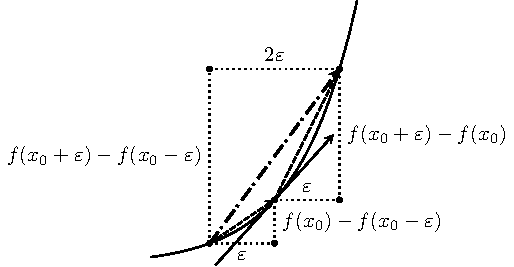
\includegraphics[width=.6\textwidth]{Chapters/04_GradientDescent/GD/latex/check_grad.pdf}
}
\end{figure}

Quan sát Hình~\ref{fig:explain_numgrad}, vector nét liền là đạo hàm {chính xác}
của hàm số tại điểm có hoành độ bằng $x_0$. Hai vector nét đứt thể hiện xấp xỉ
đạo hàm phía phải và phía trái. Vector chấm gạch thể hiện xấp xỉ đạo hàm hai
phía. Trong ba vector xấp xỉ đó, vector chấm gạch gần với vector nét liền nhất
nếu xét theo hướng.

Sự khác biệt giữa các phương pháp xấp xỉ còn lớn hơn nữa nếu tại điểm $x$, hàm số bị
{bẻ cong} mạnh hơn. Khi đó, xấp xỉ trái và phải sẽ khác nhau rất nhiều.
Xấp xỉ hai phía sẽ cho kết quả ổn định hơn.

% Từ đó ta thấy rằng xấp xỉ đạo hàm hai phía là xấp xỉ tốt hơn.

% \textbf{Với hàm nhiều biến}
\subsection{Xấp xỉ gradient của hàm nhiều biến}

Với hàm nhiều biến, công thức~\eqref{eqn:numgrdef2} được áp dụng cho từng biến
khi các biến khác cố định. Cụ thể, ta sử dụng định nghĩa gradient của hàm số nhận
đầu vào là một ma trận như công thức~\eqref{eqn:grmatrix1}. Mỗi thành phần của
ma trận kết quả là đạo hàm riêng của hàm số tại thành phần đó khi ta coi các thành
phần còn lại cố định. Chúng ta sẽ thấy rõ điều này hơn ở cách lập trình so sánh
hai cách tính gradient ngay sau đây.

Cách tính gradient xấp xỉ hai phía thường cho giá trị khá chính xác. Tuy nhiên,
cách này không được sử dụng để tính gradient vì độ phức tạp quá cao so với cách
tính trực tiếp. Tại mỗi thành phần, ta cần tính giá trị của hàm số tại phía trái
và phía phải. Việc làm này không khả thi với các ma trận lớn. Khi so sánh đạo
hàm xấp xỉ với gradient tính theo công thức, người ta thường giảm số chiều dữ
liệu và giảm số điểm dữ liệu để thuận tiện cho tính toán. Nếu gradient tính được
là chính xác, nó sẽ rất gần với gradient xấp xỉ này.

Đoạn code dưới đây giúp kiểm tra gradient của một hàm số khả vi $f:
\R^{m \times n} \rightarrow \R$, có kèm theo hai ví dụ. Để sử dụng hàm kiểm tra
\pythoninline{check_grad} này, ta cần viết hai hàm. Hàm thứ nhất là hàm
\pythoninline{fn(X)} tính giá trị của hàm số tại \pythoninline{X}. Hàm thứ hai
là hàm \pythoninline{gr(X)} tính giá trị của gradient của \pythoninline{fn(X)}.

\newpage

\begin{lstlisting}[language=Python]
from __future__ import print_function
import numpy as np

def check_grad(fn, gr, X):
    X_flat    = X.reshape(-1) # convert X to an 1d array, 1 for loop needed
    shape_X   = X.shape                # original shape of X
    num_grad  = np.zeros_like(X)       # numerical grad, shape = shape of X
    grad_flat = np.zeros_like(X_flat)  # 1d version of grad
    eps       = 1e-6      # a small number, 1e-10 -> 1e-6 is usually good
    numElems  = X_flat.shape[0] # number of elements in X
    # calculate numerical gradient
    for i in range(numElems):          # iterate over all elements of X
        Xp_flat      = X_flat.copy()
        Xn_flat      = X_flat.copy()
        Xp_flat[i]  += eps
        Xn_flat[i]  -= eps
        Xp           = Xp_flat.reshape(shape_X)
        Xn           = Xn_flat.reshape(shape_X)
        grad_flat[i] = (fn(Xp) - fn(Xn))/(2*eps)

    num_grad = grad_flat.reshape(shape_X)

    diff = np.linalg.norm(num_grad - gr(X))
    print('Difference between two methods should be small:', diff)

# ==== check if grad(trace(A*X)) == A^T ====
m, n = 10, 20
A = np.random.rand(m, n)
X = np.random.rand(n, m)

def fn1(X):
    return np.trace(A.dot(X))

def gr1(X):
    return A.T

check_grad(fn1, gr1, X)
# ==== check if grad(x^T*A*x) == (A + A^T)*x  ====
A = np.random.rand(m, m)
x = np.random.rand(m, 1)

def fn2(x):
    return x.T.dot(A).dot(x)

def gr2(x):
    return (A + A.T).dot(x)

check_grad(fn2, gr2, x)

\end{lstlisting}
% \newpage
\kq
\begin{lstlisting}
Difference between two methods should be small: 2.02303323394e-08
Difference between two methods should be small: 2.10853872281e-09
\end{lstlisting}

Kết quả cho thấy sự khác nhau giữa Frobenious norm (norm mặc định trong
\pythoninline{np.linalg.norm}) trong kết quả của hai cách tính là rất nhỏ. Sau
khi chạy lại đoạn code với các giá trị \pythoninline{m, n} khác nhau và biến
\pythoninline{X} khác nhau, nếu sự khác nhau vẫn là nhỏ, ta có thể kết luận rằng
gradient mà ta tính được là chính xác.

Bạn đọc có thể kiểm tra lại các công thức trong Bảng~\ref{tab:commongr} bằng
phương pháp này.




%!TEX root = ../../book_ML.tex
\chapter{Ôn tập Xác suất}
\label{cha:prob}
%  -- -
% \textbf{Trong trang này:}


% - \href{http://machinelearningcoban.com#-gioi-thieu}{1. Giới thiệu}
% - \href{http://machinelearningcoban.com#-xac-suat}{2. Xác Suất}
%   - \href{http://machinelearningcoban.com#-random-variables}{2.1. Random variables}
%   - \href{http://machinelearningcoban.com#-joint-probability}{2.2. Joint probability}
%   - \href{http://machinelearningcoban.com#-marginalization}{2.3. Marginalization}
%   - \href{http://machinelearningcoban.com#-conditional-probability}{2.4. Conditional probability}
%   - \href{http://machinelearningcoban.com#-quy-tac-bayes}{2.5. Quy tắc Bayes}
%   - \href{http://machinelearningcoban.com#-independence}{2.6. Independence}
%   - \href{http://machinelearningcoban.com#-ky-vong}{2.7. Kỳ vọng}
% - \href{http://machinelearningcoban.com#-mot-vai-xac-suat-thuong-gap}{3. Một vài xác suất thường gặp}
%   - \href{http://machinelearningcoban.com#-bernouli-distribution}{3.1. Bernoulli distribution}
%   - \href{http://machinelearningcoban.com#-categorical-distribution}{3.2. categorical distribution}
%   - \href{http://machinelearningcoban.com#-univariate-normal-distribution-phan-phoi-chuan-mot-bien}{3.3. Univariate normal distribution $Phân phối chuẩn một biến$}
%   - \href{http://machinelearningcoban.com#-multivariate-normal-distribution}{3.4. Multivariate normal distribution}
%   - \href{http://machinelearningcoban.com#-beta-distribution}{3.5. Beta distribution}
%   - \href{http://machinelearningcoban.com#-dirichlet-distribution}{3.6. Dirichlet distribution}
% - \href{http://machinelearningcoban.com#-thao-luan}{4. Thảo luận}
% - \href{http://machinelearningcoban.com#-tai-lieu-tham-khao}{5. Tài liệu tham khảo}



% \section{Giới thiệu}

% Cho tới thời điểm này, kế hoạch viết về phần Machine Learning cơ bản của tôi đã thực hiện được 1 nửa. Trong nửa đầu của blog, các bạn đã làm quen (lại) rất nhiều với Đại số tuyến tính và Tối ưu.

% Nhìn chung, tôi đều viết các thuật toán Machine Learning dưới dạng các bài toán tối ưu và cách giải mỗi bài toán đó.

% Các bài viết trong nửa đầu có thể chia thành các Phần:

% 1. Bài 1-6: Làm quen với Machine Learning. Một vài thuật toán Machine Learning cơ bản chưa cần nhiều tới tối ưu.

% 2. Bài 7-8: Gradient Descent. Thuật toán tối ưu đơn giản mà hiệu quả cho các bài toán tối ưu không ràng buộc.

% 3. Bài 9-15: Neural Networks. Phần này giúp các bạn nắm được các thành phần cơ bản của một Neural Network và các Networks cơ bản nhất, chủ yếu cho các bài toán classification. Các bài toán tối ưu đều là không ràng buộc, các hàm mất mát hầu hết là không lồi, nghiệm tìm được là các local optimal.

% 4. Bài 16-18: Convex Optimization. Phần này bắt đầu sâu hơn một chút về Tối ưu. Định nghĩa về tập lồi, hàm lồi, bài toán tối ưu lồi và bài toán đối ngẫu. Đây là nền tảng cho rất nhiều thuật toán cơ bản Machine Learning sau này.

% 5. Bài 19-22: Support Vector Machine. Đây là một trong những thuật toán đẹp nhất và 'intuitive' nhất trong Machine Learning. Nếu bạn vào wiki tìm 'Machine Learning' thì sẽ thấy hình đại diện chính là SVM và Kernel SVM. Một trong những điều lý thú của SVM là bài toán tối ưu là lồi và nghiệm tìm được là duy nhất, cũng là global optimal.

% 6. Bài 23-25: Recommendation Systems. Đây là một lớp các bài toán thực tế và quan trọng của Machine Learning. Tôi chủ động thêm phần này vào vì làm giảm lượng toán đã đề cập quá nhiều trong Phần 4 và 5. Các thuật toán và bài toán trong phần này khá đơn giản nhưng kết quả khá tốt.

% 7. Bài 26-29: Dimensionality Reduction. Phần này cũng rất quan trọng trong Machine Learning. PCA gần như được dùng trong hầu hết các bài toán ML, trong khi LDA hiệu quả trong các bài toán classification. SVD, sau này các bạn sẽ thấy, được dùng rất nhiều vì những tính chất đẹp của nó.

% Trong nửa còn lại, tôi sẽ đi vào một mảng lớn khác của ML trong đó các kiến thức về xác suất thống kê được áp dụng rất nhiều, tôi tạm gọi phần này là Bayesian Machine Learning. Các bạn sẽ từ từ được ôn lại kiến thức về Xác Suất Thống Kê và làm quen với các thuật toán Machine Learning cơ bản khác.

% Trong bài viết này, tôi sẽ ôn tập lại những kiến thức về Xác Suất thường được sử dụng trong Machine Learning. Mục 2 sẽ nhắc lại về biến ngẫu nhiên, xác suất đồng thời, xác suất biên, xác suất có điều kiện, và quy tắc Bayes. Mục 3 sẽ nhác lại một vài phân bố xác suất thường dùng.

{Chương này được viết dựa trên Chương 2 và 3 của cuốn \textit{Computer Vision:  Models, Learning, and Inference -- Simon J.D. Prince} (\url{https://goo.gl/GTEXzd}).}

\section{Xác suất}


\subsection{Biến ngẫu nhiên}
\index{biến ngẫu nhiên -- random variable}
\index{random variable -- biến ngẫu nhiên}
\index{phân phối xác suất -- probability distribution}
\index{probability distribution -- phân phối xác suất}
% \index{random variable!}

Một \textit{biến ngẫu nhiên} (random variable) $x$ là một biến dùng để đo những đại lượng không
xác định. Biến này có thể được dùng để ký hiệu kết quả/đầu ra của một thí
nghiệm, ví dụ như tung đồng xu, hoặc một đại lượng biến đổi trong tự nhiên, ví
dụ như nhiệt độ trong ngày. Nếu quan sát một số lượng lớn đầu ra
$\{x_i\}_{i=1}^I$ của các thí nghiệm này, ta có thể nhận được những giá trị khác
nhau ở mỗi thí nghiệm. Tuy nhiên, sẽ có những giá trị xảy ra nhiều lần hơn những
giá trị khác, hoặc xảy ra gần một giá trị này hơn những giá trị khác. Thông tin
về đầu ra này được đo bởi một \textit{phân phối xác suất} (probability distribution) được biểu diễn bằng
một hàm $p(x)$. Một biến ngẫu nhiên có thể là {rời rạc} hoặc {liên
tục}.

Một biến ngẫu nhiên rời rạc sẽ lấy giá trị trong một tập hợp các điểm rời rạc
cho trước. Ví dụ tung đồng xu thì có hai khả năng là \textit{xấp} và
\textit{ngửa}. Tập các giá trị này có thể có thứ tự như khi tung xúc xắc hoặc
không có thứ tự như khi đầu ra là các giá trị \textit{nắng}, \textit{mưa},
\textit{bão}. Mỗi đầu ra có một giá trị xác suất tương ứng với nó. Các giá trị
xác suất này không âm và có tổng bằng một.
\begin{equation}
\label{eqn:30_1}
\text{Nếu}~ x ~\text{là biến ngẫu nhiên rời rạc thì}\quad \sum_{x} p(x) = 1.
\end{equation}
Biến ngẫu nhiên liên tục lấy giá trị là các số thực. Những giá trị này có thể là
hữu hạn, ví dụ thời gian làm bài của mỗi thí sinh trong một bài thi 180 phút,
hoặc vô hạn, ví dụ thời gian phải chờ tới khách hàng tiếp theo. Không như biến
ngẫu nhiên rời rạc, xác suất để đầu ra bằng {chính xác} một giá trị nào đó theo
lý thuyết là bằng không. Thay vào đó, phân phối của biến ngẫu nhiên rời rạc
thường được xác định dựa trên xác suất để đầu ra rơi vào một khoảng giá trị nào
đó. Việc này được mô tả bởi một hàm số được gọi là \textit{hàm mật độ xác suất} (probability density function, pdf). Hàm mật độ xác suất
luôn cho giá trị dương, và tích phân của nó trên toàn miền giá trị đầu ra phải
bằng một.
\index{hàm mật độ xác suất -- probability density function}
\index{probability density function -- hàm mật độ xác suất}
\index{pdf}
\begin{equation}
\label{eqn:30_2}
\text{Nếu}~ x ~\text{là biến ngẫu nhiên liên tục thì} \int p(x)dx = 1.
\end{equation}
% Để giảm thiểu ký hiệu, hàm mật độ xác suất của một biến ngẫu nhiên liên tục
% $x$ cũng được ký hiệu là $p(x)$.

\begin{mynote}
Nếu $x$ là một biến ngẫu nhiên rời rạc thì $p(x) \leq 1,~\forall x$. Trong khi
đó, nếu $x$ là biến ngẫu nhiên liên tục, $p(x)$ có thể nhận giá trị không âm
bất kỳ, điều này vẫn đảm bảo tích phân của hàm mật độ xác suất theo toàn
bộ giá trị của $x$ bằng một.    % Với biến ngẫu nhiên rời rạc, $p(x)$ được
% hiểu là \textit{mật độ xác suất} tại $x$.
\end{mynote}


\subsection{Xác suất đồng thời}
\index{xác suất đồng thời -- joint probability}
\index{joint probability -- xác suất đồng thời}
% \subsection{Joint probability}
Nếu quan sát số lượng lớn các cặp đầu ra của hai biến ngẫu nhiên $x$ và $y$ thì
có những cặp đầu ra xảy ra thường xuyên hơn những cặp khác. Thông tin này được
biểu diễn bằng một phân phối được gọi là \textit{xác suất đồng thời} (joint probability) của $x$ và
$y$, được ký hiệu là $p(x, y)$. Hai biến ngẫu nhiên $x$ và $y$ có thể cùng là
biến ngẫu nhiên rời rạc, liên tục, hoặc một rời rạc, một liên tục. Luôn nhớ rằng
tổng các xác suất trên mọi cặp giá trị $(x, y)$ đều bằng một.
\begin{align}
\text{Cả $x$ và $y$ là rời rạc:}  & &\sum_{x, y} p(x, y) &= 1. \\\
\text{Cả $x$ và $y$ là liên tục:} & &\int p(x, y) dx dy &=1.\\\
x ~\text{rời rạc}, ~ y ~\text{liên tục:} & &\sum_{x} \int p(x, y) dy &= \int \left(\sum_{x} p(x, y) \right)dy = 1.
\end{align}
Xét ví dụ trong Hình \ref{fig:30_1}, phần ``Xác suất đồng thời''. Biến ngẫu nhiên
$x$ thể hiện điểm thi môn Toán của học sinh ở một trường THPT trong một kỳ thi
quốc gia, biến ngẫu nhiên $y$ thể hiện điểm thi môn Vật Lý cũng trong kỳ thi đó.
Đại lượng $p(x = x^*, y = y^*)$ là tỉ lệ giữa tần suất số học sinh được
\textit{đồng thời} $x^*$ điểm môn Toán và $y^*$ điểm môn Vật lý với
toàn bộ số học sinh của trường đó. Tỉ lệ này có thể coi là xác suất khi số học
sinh trong trường là lớn. Ở đây $x^*$ và $y^*$ là các số xác định. Thông thường,
xác suất này được viết gọn lại thành $p(x^*, y^*)$, và $p(x, y)$ được dùng như
một hàm tổng quát để mô tả các xác suất.

Giả sử thêm rằng điểm các môn là các số tự nhiên từ 1 đến 10.

Các ô vuông màu đen thể hiện xác suất $p(x, y)$, với diện tích ô vuông càng lớn
biểu thị xác suất càng cao. Chú ý rằng tổng các xác suất này bằng một.

{Có thể thấy rằng xác suất để một học sinh được 10 điểm môn Toán
và 1 điểm môn Lý rất thấp, điều tương tự xảy ra với 10 điểm môn Lý và 1 điểm môn
Toán. Xác suất để một học sinh được khoảng 7 điểm cả hai môn là cao
nhất.}

% <hr>
% <div class="imgcap">
% <img src ="/assets/30_prob/joint.png" align = "center" width = "800">
% </div>

% <br>
% <div  class = "thecap" style = "text-align: justify" >Hình 1: Joint probability (phần trung tâm có nền mùa lục nhạt), Marginalization (phía trên và bên trái) và Conditional probability (phía dưới và bên phải).</div>
% <hr>

\begin{figure}[t]
\centering
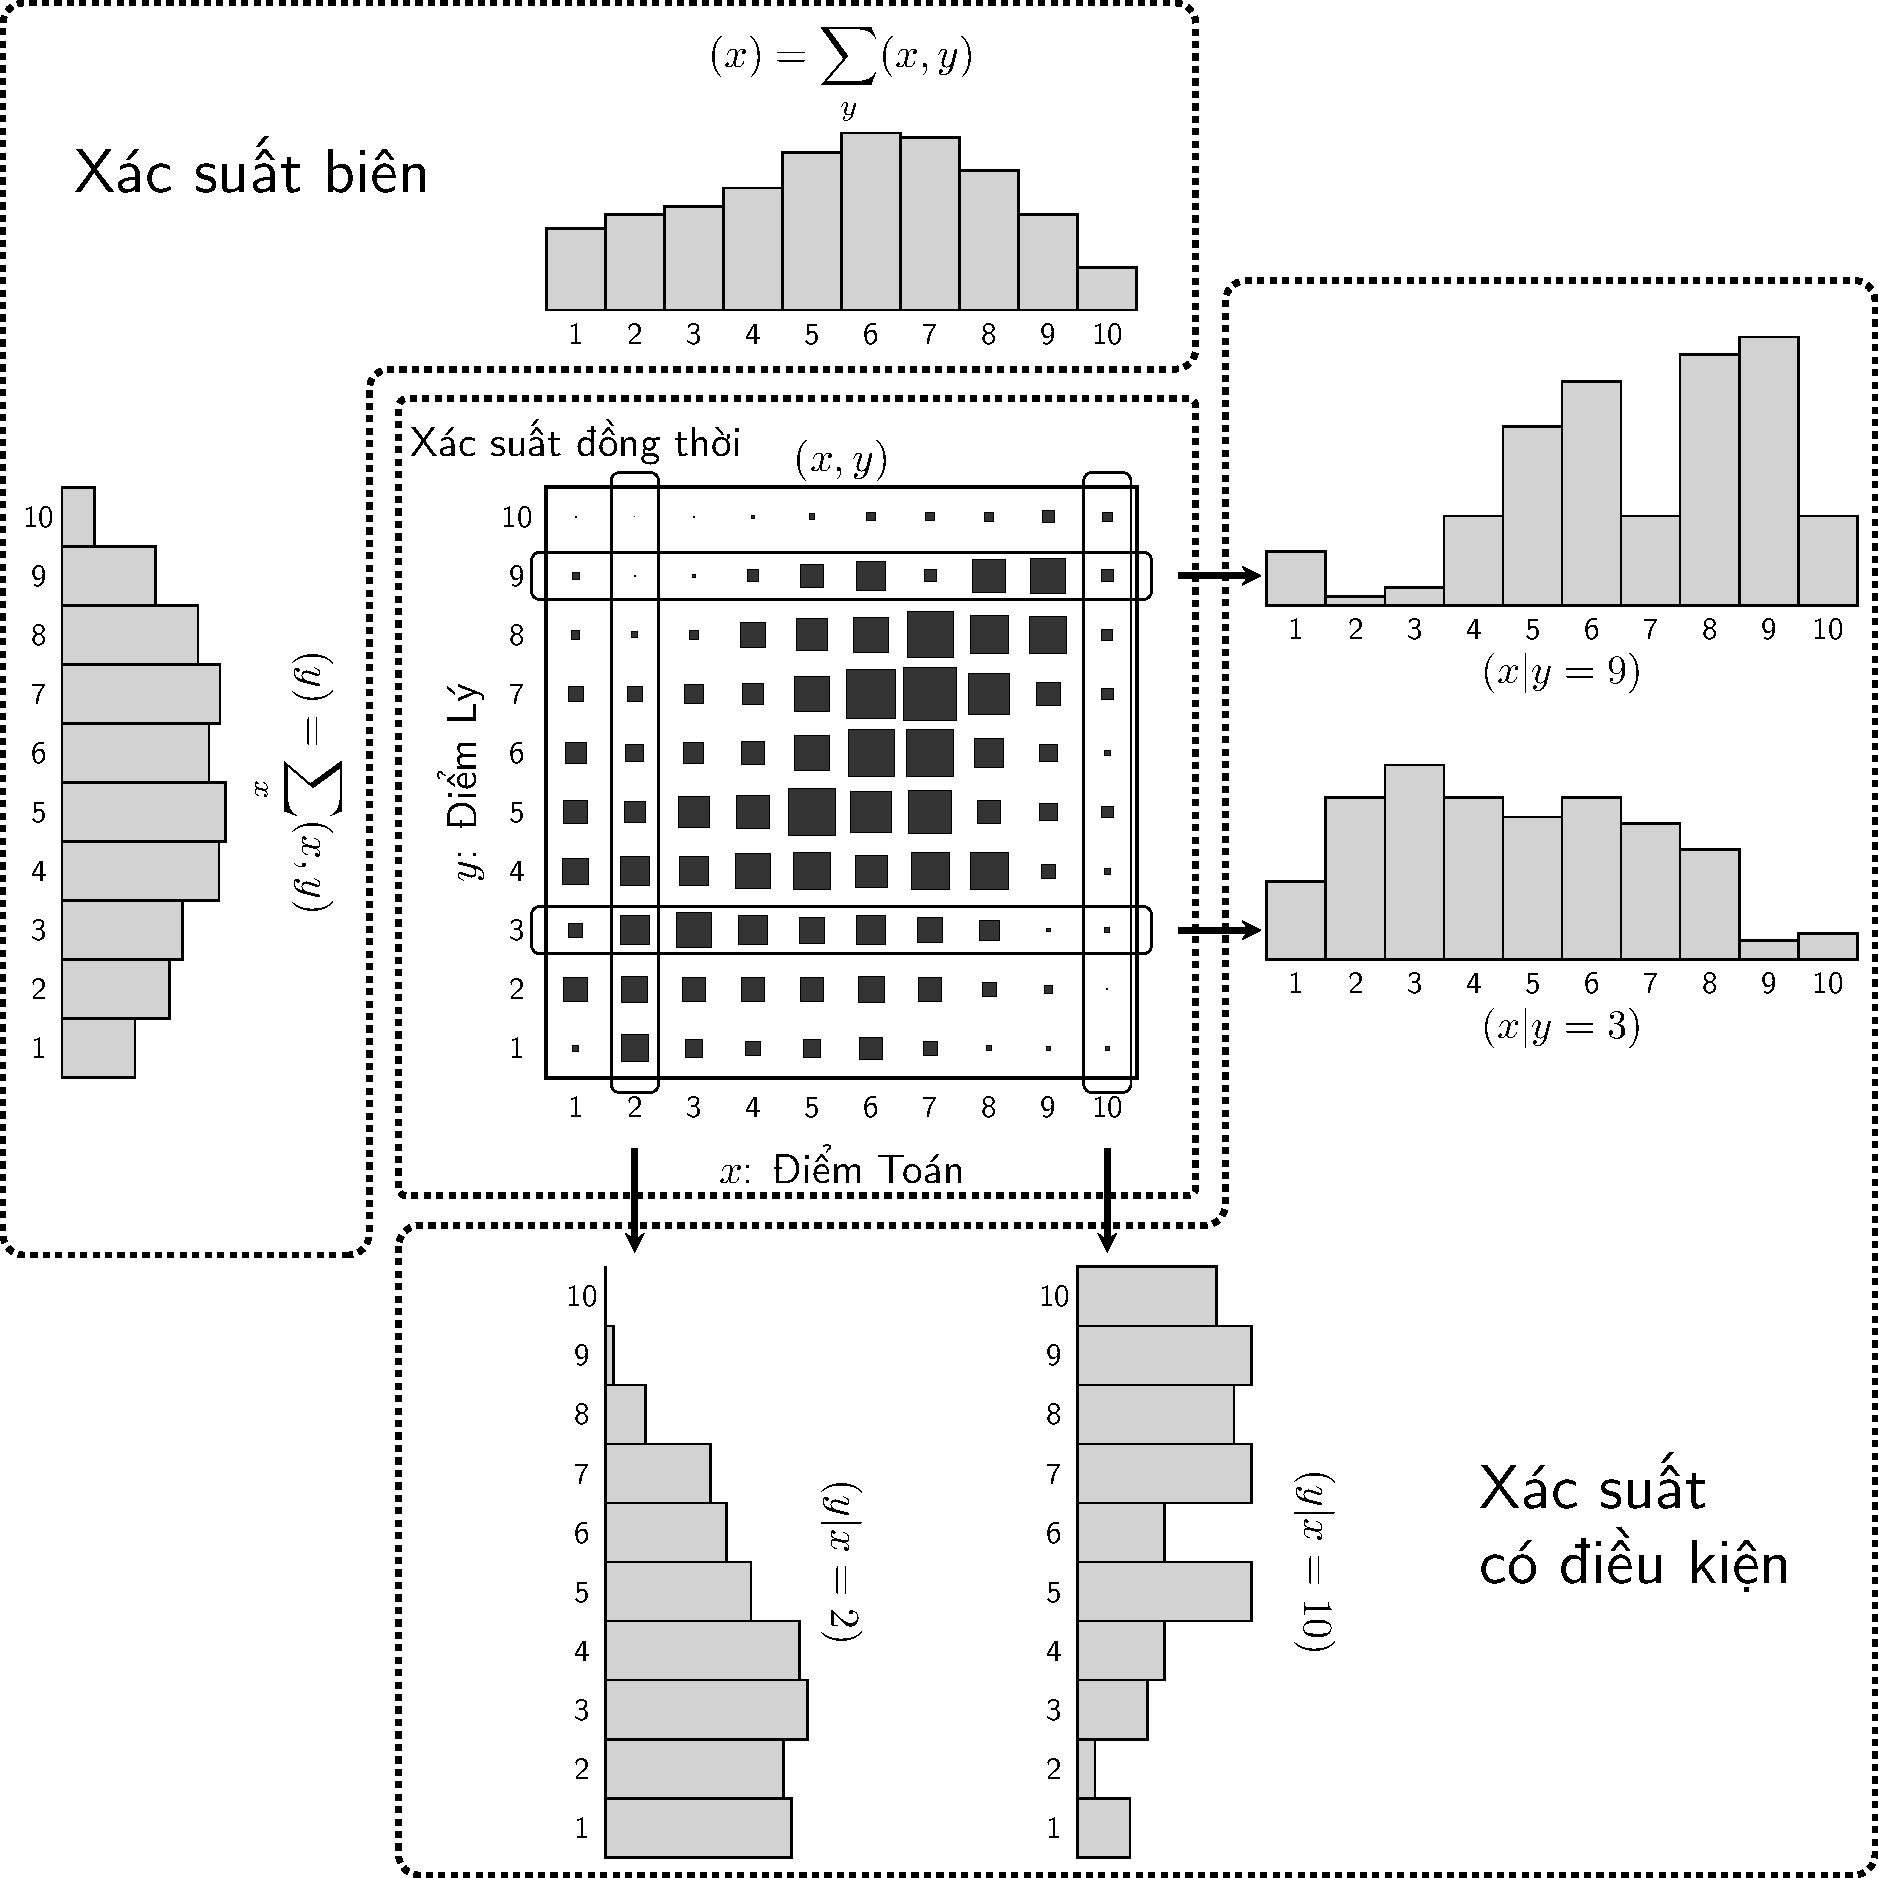
\includegraphics[width = \textwidth]{Chapters/02_LinearAlgebra/30_prob/latex/joint.pdf}
\caption[]{Xác suất đồng thời, xác suất biên, xác suất có điền kiện và mối quan hệ giữa chúng}
\label{fig:30_1}
\end{figure}

Thông thường, chúng ta sẽ làm việc với các bài toán ở đó xác suất được xác định
trên nhiều hơn hai biến ngẫu nhiên. Chẳng hạn, $p(x, y, z)$ thể hiện xác suất
đồng thời của ba biến ngẫu nhiên $x,y$ và $z$. Khi có nhiều biến ngẫu nhiên, ta
có thể viết chúng dưới dạng vector. Cụ thể, ta có thể viết $p(\mathbf{x})$ để
thể hiện xác suất của biến ngẫu nhiên nhiều chiều $\mathbf{x} =
[x_1, x_2, \dots, x_n]^T$. Khi có nhiều tập các biến ngẫu nhiên, ví dụ
$\mathbf{x}$ và $\mathbf{y}$, ta có thể viết $p(\mathbf{x},
\mathbf{y})$ để thể hiện xác suất đồng thời của tất cả các thành phần trong
hai biến ngẫu nhiên nhiều chiều này.

\subsection{Xác suất biên}
\index{xác suất biên -- marginalization}
\index{marginalization -- xác suất biên}
Nếu biết xác suất đồng thời của nhiều biến ngẫu nhiên, ta cũng có thể xác định
được phân phối xác suất của từng biến bằng cách lấy tổng (với biến ngẫu nhiên rời
rạc) hoặc tích phân (với biến ngẫu nhiên liên tục) theo tất cả các biến còn lại:% \begin{equation}
\begin{align}
\label{eqn:30_3}
\text{Nếu} ~x, y ~\text{rời rạc:}~ &p(x) = \sum_{y}p(x, y), \\
\label{eqn:30_4}
&p(y) = \sum_{x}p(x, y). \\
\label{eqn:30_5}
\text{Nếu} ~x, y ~\text{liên tục:}~ &p(x) = \int p(x, y)dy, \\
\label{eqn:30_6}
&p(y) = \int p(x, y)dx.
\end{align}
% \end{equation}
Với nhiều biến hơn, chẳng hạn bốn biến rời rạc $x, y, z, w$, cách tính được thực
hiện tương tự:
\index{xác suất biên -- marginal probability}
\index{marginal probability -- xác suất biên}
% \begin{equaton}
\begin{align}
\label{eqn:30_7}
p(x) &= \sum \limits_{ y, z, w}p(x, y, z, w),\\
\label{eqn:30_8}
p(x, y) &= \sum \limits_{z, w}p(x, y, z, w).
\end{align}
Cách xác định xác suất của một biến dựa trên xác suất đồng thời của nó với các
biến khác được gọi là \textit{phép biên hoá} (marginalization). Xác suất đó được gọi là
\textit{xác suất biên} (marginal probability).

\index{phép biên hóa -- marginalization}
\index{marginalization -- phép biên hóa}

Từ đây trở đi, nếu không đề cập gì thêm, chúng ta sẽ dùng ký hiệu $\sum$ để chỉ
chung cho cả hai loại biến ngẫu nhiên rời rạc và liên tục. Nếu biến là liên tục,
ta sẽ ngầm hiểu rằng dấu tổng ($\sum$) cần được thay bằng dấu tích phân
($\int$), biến lấy vi phân chính là biến được viết dưới dấu $\sum$. Chẳng hạn,
trong~\eqref{eqn:30_8}, nếu $z$ là liên tục, $w$ là rời rạc, công thức đúng sẽ
là
\begin{equation}
p(x, y) = \sum_{w}\left( \int p(x, y, z, w)dz \right) = \int \left( \sum_{w} p(x, y, z, w)\right) dz.
\end{equation}
Quay lại ví dụ trong Hình~\ref{fig:30_1} với hai biến ngẫu nhiên rời rạc $x, y$.
Lúc này, $p(x)$ được hiểu là xác suất để một học sinh đạt được $x$ điểm môn
Toán. Xác suất này được biểu thị ở khu vực ``Xác suất biên''. Có hai cách tính
xác suất này. Cách thứ nhất là đếm số học sinh được $x$ điểm môn toán rồi chia
cho tổng số học sinh. Cách thứ hai dựa trên xác suất đồng thời để một học sinh
được $x$ điểm môn Toán và $y$ điểm môn Lý. Số lượng học sinh đạt $x = x^*$ điểm
môn Toán sẽ bằng tổng số học sinh đạt $x = x^*$ điểm môn Toán \textit{và} $y$
điểm môn Lý, với $y$ là một giá trị bất kỳ từ 1 đến 10. vì vậy, để tính xác suất
$p(x)$, ta chỉ cần tính tổng của toàn bộ $p(x, y)$ với $y$ chạy từ 1 đến 10.

Dựa trên nhận xét này, mỗi giá trị của $p(x)$ chính bằng tổng các giá trị trong
cột thứ $x$ của hình vuông trung tâm. Mỗi giá trị của $p(y)$ sẽ bằng tổng các
giá trị trong hàng thứ $y$ tính từ đưới lên của hình vuông đó. Chú ý rằng tổng
các xác suất luôn bằng một.


\subsection{Xác suất có điều kiện.}
\index{xác suất có điều kiện -- conditional probability}
\index{conditional probability -- xác suất có điều kiện}

{Dựa vào phân phối điểm của các học sinh, liệu ta có thể tính được xác suất để
một học sinh được điểm 10 môn Lý, biết rằng học sinh đó được điểm 1 môn Toán?}

Xác suất để một biến ngẫu nhiên $x$ nhận một giá trị nào đó biết
rằng biến ngẫu nhiên $y$ có giá trị $y^*$ được gọi là \textit{xác suất có điều
kiện} (conditional probability), ký hiệu là $p(x| y = y^*)$.
% (đọc là \textit{probability of $x$ given that $y$ takes value $y^*$}).


Xác suất có điều kiện $p(x | y = y^*)$ có thể được tính dựa trên xác suất đồng
thời $p(x, y)$. Quay lại Hình~\ref{fig:30_1} ở khu vực ``Xác suất có điều
kiện''. Nếu biết rằng $y = 9$, xác suất $p(x | y = 9)$ có thể tính được dựa trên
hàng thứ chín của hình vuông trung tâm, tức hàng $p(x, y = 9)$. Xác suất $p(x | y =
9) $ lớn nếu $p(x, y= 9)$ lớn. Chú ý rằng tổng các xác suất $\sum_{x} p(x,
y = 9)$ nhỏ hơn một, và bằng tổng các xác suất trên hàng thứ chín này. Để thoả
mãn điều kiện tổng các xác suất bằng một, ta cần chia mỗi đại lượng $p(x, y =
9)$ cho tổng của hàng này, tức là
\begin{equation}
p(x | y = 9) =\frac{p(x, y = 9)}{\sum \limits_x p(x, y = 9)} =
\frac{p(x, y = 9)}{p(y = 9)}.
\end{equation}
Tổng quát,
\begin{equation}
\label{eqn:30_9}
\displaystyle
p(x|y = y^*) = \frac{p(x, y = y^*)}{\sum \limits_{x} p(x, y = y^*)} =
\frac{p(x, y = y^*)}{p(y = y^*)},
\end{equation}
ở đây ta đã sử dụng công thức tính xác suất biên trong~\eqref{eqn:30_4} cho mẫu
số. Thông thường, ta có thể viết xác suất có điều kiện mà không cần chỉ rõ giá trị $y = y^*$ và có các công thức gọn hơn:
\begin{equation}
\label{eqn:30_2}
p(x |y) = \frac{p(x, y)}{p(y)}, ~p(y | x) = \frac{p(y, x)}{p(x)}.
\end{equation}

Từ đó ta có quan hệ
\begin{equation}
\label{eqn:30_11}
p(x, y) = p(x|y)p(y) = p(y | x) p(x).
\end{equation}
Khi có nhiều hơn hai biến ngẫu nhiên, ta có các công thức
\begin{eqnarray}
\label{eqn:30_12}
p(x, y, z, w)
& = & p(x, y, z | w) p(w) \\
\label{eqn:30_13}
& = & p(x, y | z, w)p(z, w) = p(x, y | z, w) p(z | w) p(w) \\
\label{eqn:30_14}
& = & p(x | y, z, w)p(y | z, w) p(z | w) p(w).
\end{eqnarray}

Công thức \eqref{eqn:30_14} có dạng {chuỗi} và được sử dụng nhiều sau
này.


\subsection{Quy tắc Bayes}
\index{quy tắc Bayes -- Bayes' rule}
\index{Bayes' rule -- quy tắc Bayes}
Công thức \eqref{eqn:30_11} biểu diễn xác suất đồng thời theo hai cách. Từ đó có thể suy ra
\begin{equation}
p(y |x) p(x) = p(x | y) p(y).
\end{equation}
Biến đối một chút:
% \begin{equation}
% \displaystyle
\begin{align}
\label{eqn:30_15}
p(y | x)
& =  \frac{p(x |y) p(y)}{p(x)} \\
\label{eqn:30_16}
& =  \frac{p(x |y) p(y)}{\sum \limits_{y} p(x, y)} \\
\label{eqn:30_17}
& =  \frac{p(x |y) p(y)}{\sum \limits_{y} p(x | y) p(y)}.
\end{align}
% \end{equation}
Trong dòng thứ hai và thứ ba, các công thức về xác suất biên và xác suất đồng thời
ở mẫu số đã được sử dụng. Từ~\eqref{eqn:30_17} ta có thể thấy rằng $p(y | x)$
hoàn toàn có thể tính được nếu ta biết mọi $p(x | y)$ và $p(y)$. Tuy nhiên, việc
tính trực tiếp xác suất này thường phức tạp.

% Thay vào đó, ta có thể đi tìm mô
% hình phù hợp của $p(\mathbf{x} | y)$ trên training data sao cho \textit{những gì
% đã thực sự xảy ra có xác suất cao nhất có thể} (Chỗ này có thể hơi khó hình
% dung, tôi sẽ nói cụ thể về việc này trong bài tiếp theo). Dựa trên training
% data, các tham số của mô hình này có thể tìm được qua một bài toán tối ưu.

{Ba công thức \eqref{eqn:30_15}-\eqref{eqn:30_17} thường được gọi là \textit{quy
tắc Bayes}. Chúng được sử dụng rộng rãi trong machine learning}

% Trong Machine Learning, chúng ta thường mô tả quan hệ giữa hai biến $x$ và $y$
% dưới dạng xác suất có điều kiện $p(y|x)$. Ví dụ, biết rằng đầu vào là một bức
% ảnh ở dạng vector $\mathbf{x}$, xác suất để bức ảnh chứa một chiếc xe là bao nhiêu. Khi đó, ta phải tính $p(y | \mathbf{x})$.

% \textbf{Ví dụ}: Tại một bệnh viện, giả sử chúng ta quan tâm tới việc xét nghiệm
% một bệnh nhân có
% bệnh ung thư phổi hay không nếu anh/cô ấy hút thuốc. Biết rằng xác xuất một
% bệnh nhân vào xét nghiệm trong bệnh viện đó có bệnh ung thư phổi là 0.1.


\subsection{Biến ngẫu nhiên độc lập}
\index{biến ngẫu nhiên độc lập -- independent random variables}
\index{independent random variables -- biến ngẫu nhiên độc lập}
Nếu biết giá trị của một biến ngẫu nhiên $x$ không mang lại thông tin về việc
suy ra giá trị của biến ngẫu nhiên $y$ và ngược lại, thì ta nói rằng hai biến
ngẫu nhiên này là \textit{độc lập}. Chẳng hạn, chiều cao của một học sinh và
điểm thi môn Toán của học sinh đó có thể coi là hai biến ngẫu nhiên {độc lập}.
Khi hai biến ngẫu nhiên $x$ và $y$ là {độc lập}, ta  có% \begin{equation}
\begin{eqnarray}
\label{eqn:30_18}
p(x | y) &=& p(x),  \\
\label{eqn:30_19}
p(y | x) &=& p(y).
\end{eqnarray}
% \end{equation}
Thay vào biểu thức xác suất đồng thời trong \eqref{eqn:30_11}, ta có
\begin{equation}
\label{eqn:30_20}
p(x, y) = p(x | y) p(y) = p(x) p(y).
\end{equation}


\subsection{Kỳ vọng}
\label{sub:expectaion_covariance}
\index{kỳ vọng -- expectation}
\index{expectation -- kỳ vọng}
\textit{Kỳ vọng} (expectation) của một biến ngẫu nhiên $x$ được định nghĩa bởi% \begin{equation}
\begin{eqnarray}
\label{eqn:30_21}
\text{E}[x] = \sum_x x p(x)  & \text{nếu}~ x ~ \text{là rời rạc.} \quad
\\
\label{eqn:30_22}
\text{E}[x] = \int x p(x) dx  & \text{nếu}~ x ~ \text{là liên tục.}
\end{eqnarray}
% \end{equation}
Giả sử $f(.)$ là một hàm số trả về một số với mỗi giá trị $x^*$ của biến ngẫu
nhiên $x$. Khi đó, nếu $x$ là biến ngẫu nhiên rời rạc, ta có
\begin{equation}
\label{eqn:30_23}
\text{E}[f(x)] = \sum_x f(x) p(x).
\end{equation}
Công thức cho biến ngẫu nhiên liên tục cũng được viết tương tự.

Với xác suất đồng thời, kỳ vọng của một hàm cũng được xác định tương tự:
\begin{equation}
\label{eqn:30_24}
\text{E}[f(x, y)] = \sum_{x,y} f(x, y) p(x, y) dx dy.
\end{equation}
Có ba tính chất cần nhớ về kỳ vọng:
\begin{enumerate}
\item Kỳ vọng của một hằng số theo một biến ngẫu nhiên $x$ bất kỳ bằng chính hằng số đó:
\begin{equation}
\label{eqn:30_25}
\text{E}[\alpha] = \alpha.
\end{equation}
\item Kỳ vọng có tính chất tuyến tính:
\begin{eqnarray}
\label{eqn:30_26}
\text{E}[\alpha x] & = & \alpha \text{E}[x],  \\
\label{eqn:30_27}
\text{E}[f(x) + g(x)] & = & \text{E}[f(x)] + \text{E}[g(x)].
\end{eqnarray}
\item Kỳ vọng của tích hai biến ngẫu nhiên độc lập bằng tích kỳ vọng của chúng:
\begin{equation}
\label{eqn:30_28}
\text{E}[f(x) g(y)] = \text{E}[f(x)] \text{E}[g(y)].
\end{equation}

\end{enumerate}


% \subsection{Kỳ vọng và ma trận hiệp phương sai}

Khái niệm kỳ vọng thường đi kèm với khái niệm \textit{phương
sai} (variance) trong không gian một chiều và \textit{ma trận hiệp
phương sai} (covariance matrix) trong không gian nhiều chiều.

\subsection{Phương sai} % (fold)

% \subsubsection{Với dữ liệu một chiều}
\index{phương sai -- variance}
\index{variance -- phương sai}
\index{do@độ lệch chuẩn -- standard deviation}
\index{standard deviation -- độ lệch chuẩn}
Cho $N$ giá trị $x_1, x_2, \dots, x_N$. {Kỳ vọng} và {phương sai}
của bộ dữ liệu này được tính theo công thức
\begin{eqnarray}
\bar{x} &=& \frac{1}{N}\sum_{n=1}^N x_n = \frac{1}{N}\mathbf{x1},\\\
\sigma^2 &=& \frac{1}{N} \sum_{n=1}^N (x_n - \bar{x})^2,
\end{eqnarray}
với $\bx = \bmt x_1, x_2, \dots, x_N\emt $, và $\mathbf{1} \in \mathbb{R}^N$ là
vector cột chứa toàn phần tử 1. Kỳ vọng đơn giản là trung bình cộng của toàn bộ
các giá trị. Phương sai là trung bình cộng của bình phương khoảng cách từ mỗi
điểm tới kỳ vọng. Phương sai càng nhỏ, các điểm dữ liệu càng gần với kỳ vọng,
tức các điểm dữ liệu càng giống nhau. Phương sai càng lớn, dữ liệu càng có tính
phân tán. Ví dụ về kỳ vọng và phương sai của dữ liệu một chiều có thể được thấy
trong Hình~\ref{fig:27_2a}.

Căn bậc hai của phương sai, $\sigma$ còn được gọi là \textit{độ lệch chuẩn} (standard deviation) của
dữ liệu.


%%%%%%% Three subfigures with bottom caption%%%%%%%%%%%%%%
\begin{figure}[t]
\begin{subfigure}{0.325\textwidth}
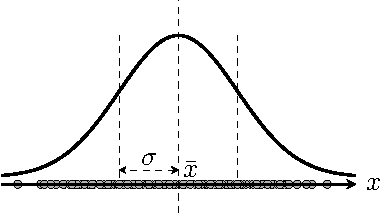
\includegraphics[width=0.99\linewidth]{Chapters/07_DimemsionalityReduction/27_pca/latex/var_1d.pdf}
\caption{}
\label{fig:27_2a}
\end{subfigure}
\begin{subfigure}{0.325\textwidth}
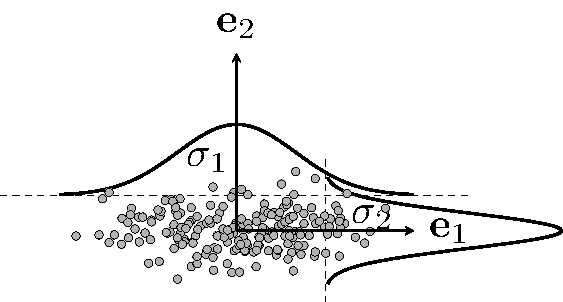
\includegraphics[width=0.99\linewidth]{Chapters/07_DimemsionalityReduction/27_pca/latex/pca_diagvar.pdf}
\caption{}
\label{fig:27_2b}
\end{subfigure}
\begin{subfigure}{0.325\textwidth}
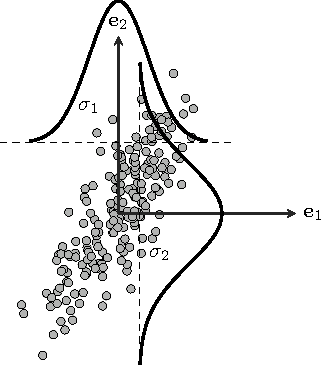
\includegraphics[width=0.99\linewidth]{Chapters/07_DimemsionalityReduction/27_pca/latex/pca_var0.pdf}
\caption{}
\label{fig:27_2c}
\end{subfigure}
\caption{
Ví dụ về kỳ vọng và phương sai. (a) Dữ liệu trong không gian
một chiều. (b) Dữ liệu trong không gian hai chiều mà hai chiều
không tương quan. Trong trường hợp này, ma trận hiệp phương sai là ma trận
đường chéo với hai phần tử trên đường chéo  là $\sigma_1, \sigma_2$, đây
cũng chính là hai trị riêng của ma trận hiệp phương sai và là phương sai
của mỗi chiều dữ liệu. (c) Dữ liệu trong không gian hai chiều có tương
quan. Theo mỗi chiều, ta có thể tính được kỳ vọng và phương sai. Phương sai
càng lớn thì dữ liệu trong chiều đó càng phân tán. Trong ví dụ này, dữ liệu
theo chiều thứ hai phân tán nhiều hơn so với chiều thứ nhất. }
\label{fig:27_2}
\end{figure}

\subsection{Ma trận hiệp phương sai}

Cho $N$ điểm dữ liệu được biểu diễn bởi các vector cột $\mathbf{x}_1, \dots, \mathbf{x}_N$, khi đó, {vector kỳ vọng} và {ma trận hiệp phương sai} của toàn bộ dữ liệu được định nghĩa là
\begin{eqnarray}
\bar{\mathbf{x}} &=& \frac{1}{N} \sum_{n=1}^N \mathbf{x}_n, \\\
\mathbf{S} &=&  \frac{1}{N}\sum_{n=1}^N (\mathbf{x}_n - \bar{\mathbf{x}})(\mathbf{x}_n - \bar{\mathbf{x}})^T = \frac{1}{N}\hat{\mathbf{X}}\hat{\mathbf{X}}^T.
\end{eqnarray}
Trong đó $\hat{\mathbf{X}}$ được tạo bằng cách trừ mỗi cột của $\mathbf{X}$ đi $\bar{\mathbf{x}}$:
\begin{equation}
\hat{\mathbf{x}}_n = \mathbf{x}_n - \bar{\mathbf{x}}.
\end{equation}
\newpage
Một vài tính chất của ma trận hiệp phương sai:
\begin{enumerate}

\item Ma trận hiệp phương sai là một ma trận đối xứng, hơn nữa, nó là một ma trận \href{https://machinelearningcoban.com/2017/03/12/convexity/#positive-semidefinite}{nửa xác định dương}.

\item Mọi phần tử trên đường chéo của ma trận hiệp phương sai là các số không âm. Chúng chính là phương sai của từng chiều dữ liệu.

\item Các phần tử ngoài đường chéo $s_{ij}, i \neq j$ thể hiện sự tương quan
giữa thành phần thứ $i$ và thứ $j$ của dữ liệu, còn được gọi là hiệp phương
sai. Giá trị này có thể dương, âm hoặc bằng không. Khi nó bằng không, ta nói
rằng hai thành phần $i, j$ trong dữ liệu là \textit{không tương quan}.

\item Nếu ma trận hiệp phương sai là ma trận đường chéo, ta có dữ liệu hoàn toàn không tương quan giữa các chiều.
\end{enumerate}

Ví dụ về sự tương quan của dữ liệu được cho trong Hình~\ref{fig:27_2b} và
\ref{fig:27_2c}.% <hr>
% <div>
% <table width = "100%" style = "border: 0px solid white">
%     <tr >
%         <td width="40%" style = "border: 0px solid white" align = "center">
%         <img style="display:block;" width = "100%" src = "/assets/27_pca/var_1d.png">
%          <br>
%         a)
%          </td>
%          <td width="40%" style = "border: 0px solid white" align = "center">
%          <img style="display:block;" width = "100%" src = "/assets/27_pca/pca_diagvar.png">
%           <br>
%          b)
%           </td>
%     </tr>

%     <tr >
%         <td width="40%" style = "border: 0px solid white" align = "center">
%         <img style="display:block;" width = "100%" src = "/assets/27_pca/pca_var0.png">
%          <br>
%         c)
%          </td>
%          <td width="40%" style = "border: 0px solid white" align = "justify">
%         Hình 2: Ví dụ về kỳ vọng và phương sai. a) Trong không gian 1 chiều. b) Không gian 2 chiều mà hai chiều không tương quan. Trong trường hợp này, ma trận hiệp phương sai là ma trận đường chéo với hai phần tử trên đường chéo  là $\sigma_1, \sigma_2$, đây cũng chính là hai trị riêng của ma trận hiệp phương sai và là phương sai của mỗi chiều dữ liệu. c) Dữ liệu trong không gian hai chiều có tương quan. Theo mỗi chiều, ta có thể tính được kỳ vọng và phương sai. Phương sai càng lớn thì dữ liệu trong chiều đó càng phân tán. Trong ví dụ này, dữ liệu theo chiều thứ hai phân tán nhiều hơn so so với chiều thứ nhất.
%           </td>
%     </tr>
% </table>
% </div>
% <hr>


\section{Một vài phân phối thường gặp}
\index{phân phối xác suất -- probability distribution}
\index{probability distribution -- phân phối xác suất}
\subsection{Phân phối Bernoulli}
\index{phân phối xác suất -- probability distribution!phân phói Bernoulli}
\index{probability distribution -- phân phối xác suất!phân phói Bernoulli}

Phân phối Bernoulli là một phân phối rời rạc mô tả các biến ngẫu nhiên nhị
phân với đầu ra chỉ nhận một trong hai giá trị $x \in \{0, 1\}$. Hai giá trị
này có thể là \textit{xấp} và \textit{ngửa} khi tung đồng xu; có thể là
\textit{giao dịch lừa đảo} và \textit{giao dịch thông thường} trong bài toán
xác
định giao dịch lừa đảo trong tín dụng; có thể là \textit{người} và \textit{không
phải người} trong bài toán xác định xem trong một bức ảnh có người hay không.

Phân phối Bernoulli được mô tả bằng một tham số $\lambda \in [0, 1]$. Xác suất của mỗi đầu ra là
\begin{equation}
\label{eqn:30_29}
p(x = 1) = \lambda, ~~~~ p(x = 0) = 1 - p(x = 1) = 1 - \lambda.
\end{equation}
Hai đẳng thức này thường được viết gọn lại thành
\begin{equation}
\label{eqn:30_292}
p(x) = \lambda^x (1 - \lambda)^{1 - x},
\end{equation}
với giả định $0 ^0 = 1$. Thật vậy, $p(0) = \lambda^0 (1 - \lambda)^1 = 1 -
\lambda$, và $p(1) = \lambda^1 (1 - \lambda)^0 = \lambda$.


Phân phối Bernoulli thường được ký hiệu ngắn gọn dưới dạng
\begin{equation}
\label{eqn:30_30}
p(x) = \text{Bern}_x [\lambda].
\end{equation}

\subsection{Phân phối categorical}
\index{phân phối xác suất -- probability distribution!phân phối categorical}
\index{probability distribution -- phân phối xác suất!phân phối categorical}
Trong nhiều trường hợp, đầu ra của biến ngẫu nhiên rời rạc có thể nhận nhiều hơn
hai giá trị. Ví dụ, một bức ảnh có thể chứa một chiếc xe, một người, hoặc một
con mèo. Khi đó, ta dùng một phân phối tổng quát của phân phối Bernoulli, được
gọi là \textit{phân phối categorical}. Các đầu ra được mô tả bởi một phần tử
trong tập hợp $\{1, 2, \dots, K\}$.

Nếu có $K$ đầu ra, phân phối categorical sẽ được mô tả bởi $K$ tham số, viết
dưới dạng vector $\lambda = [\lambda_1, \lambda_2, \dots, \lambda_K]$ với các
$\lambda_k$ không âm và có tổng bằng một. Mỗi giá trị $\lambda_k$ thể hiện xác
suất để đầu ra nhận giá trị $k$:
\begin{math}
p(x = k) = \lambda_k
\end{math}.
\index{biểu diễn one-hot -- one-hot encoding}
\index{one-hot encoding -- biểu diễn one-hot}

Phân phối categorical thường được ký hiệu dưới dạng:
\begin{equation}
p(x) = \text{Cat}_x [\lambda].
\end{equation}
Cách biểu diễn đầu ra là một số $k$ trong tập hợp $\{1, 2, \dots, K\}$ có thể
được thay bằng biểu diễn \textit{one-hot}. Mỗi vector one-hot là một vector $K$
phần tử, trong đó $K-1$ phần tử bằng 0, một phần tử bằng 1 tại vị trí ứng với
đầu ra $k$. Nói cách khác, mỗi đầu ra là một trong các vector đơn vị bậc $K$:
$\{\mathbf{e}_1, \mathbf{e}_2,\dots, \mathbf{e}_K\}$. Ta có thể viết
\begin{equation}
\label{eqn:30_31}
p(x = k) = p(\mathbf{x} = \mathbf{e}_k) = \prod_{j=1}^K \lambda_j^{x_j} = \lambda_k.
\end{equation}
Dấu bằng cuối cùng xảy ra vì $x_k = 1, x_j = 0~\forall j \neq k$.
% Cách viết này được sử dụng rất nhiều trong Machine Learning.
% Thay vào~\eqref{eqn:30_31} ta sẽ được $p(\bx = \be_k) = \lambda_k = p(x = k)$.


\subsection{Phân phối chuẩn một chiều}
\index{phân phối xác suất -- probability distribution!phân phối chuẩn một chiều -- univariate normal distribution}
\index{probability distribution -- phân phối xác suất!univariate normal distribution -- phân phối chuẩn một chiều}

\textit{Phân phối chuẩn một chiều} (univariate normal distribution) được định nghĩa trên các biến liên tục nhận giá
trị $x \in (-\infty, \infty)$. Đây là một phân phối được sử dụng nhiều nhất với
các biến ngẫu nhiên liên tục. Phân phối này được mô tả bởi hai tham số:
{kỳ vọng} $\mu$ và {phương sai} $\sigma^2$.

Hàm mật độ xác suất của phân phối này được định nghĩa bởi
\begin{equation}
\label{eqn:30_32}
p(x) = \frac{1}{\sqrt{2\pi \sigma^2}}\exp \left( -\frac{(x - \mu)^2}{2\sigma^2}\right).
\end{equation}
Hàm mật độ này thường được viết gọn dưới dạng $p(x) = \text{Norm}_x [\mu,
\sigma^2]$ hoặc $\mathcal{N}(\mu, \sigma^2)$.

Ví dụ về đồ thị hàm mật độ xác suất của phân phối chuẩn một chiều được biểu thị
trên Hình~\ref{fig:30_2a}.

\begin{figure}[t]
\begin{subfigure}{0.49\textwidth}
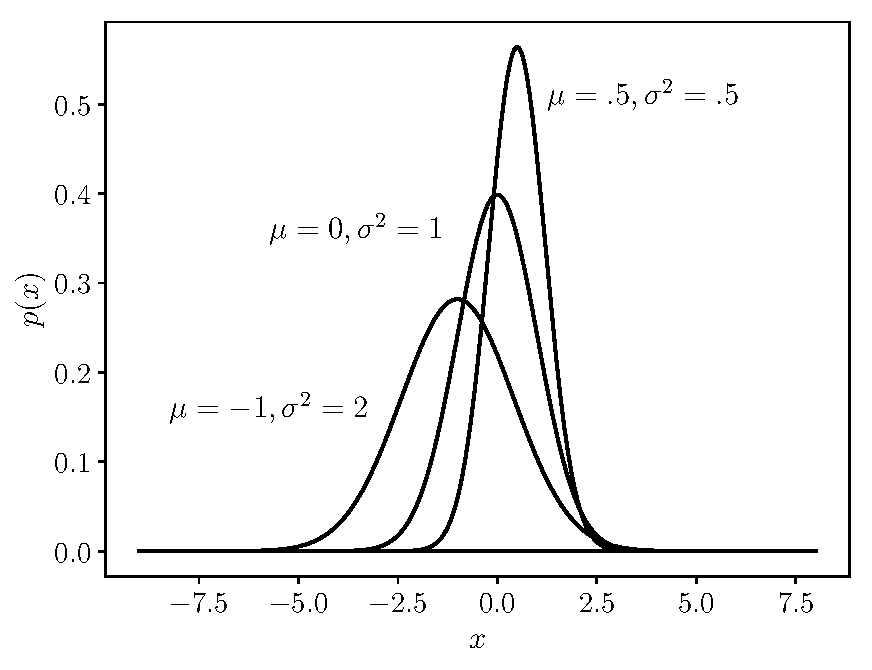
\includegraphics[width=0.99\linewidth]{Chapters/02_LinearAlgebra/30_prob/python/uni_norm.pdf}
\caption{}
\label{fig:30_2a}
\end{subfigure}
\begin{subfigure}{0.49\textwidth}
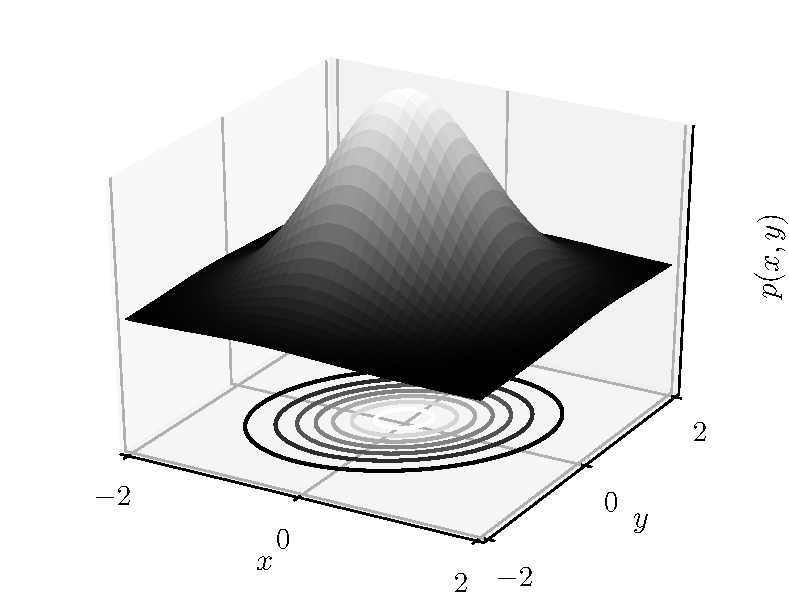
\includegraphics[width=0.99\linewidth]{Chapters/02_LinearAlgebra/30_prob/python/bi_norm.pdf}
% 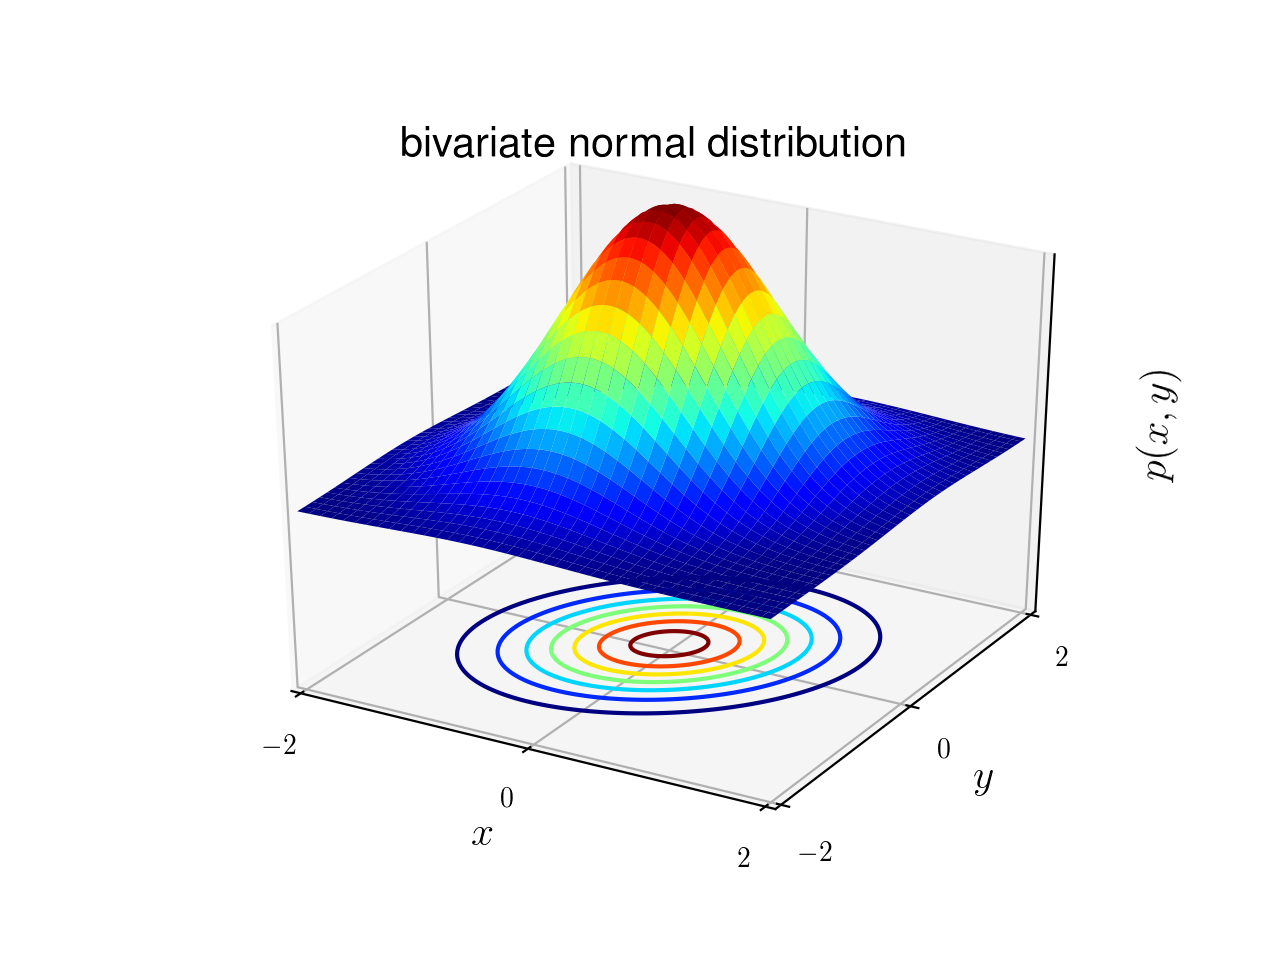
\includegraphics[width=0.99\linewidth]{Chapters/02_LinearAlgebra/30_prob/bivariate.png}
\caption{}
\label{fig:30_2b}
\end{subfigure}
\caption{
Ví dụ về hàm mật độ xác suất của (a) phân phối chuẩn một chiều, và (b) phân
phối chuẩn hai chiều.}
\label{fig:30_2}
\end{figure}

\subsection{Phân phối chuẩn nhiều chiều}
\index{phân phối xác suất -- probability distribution!phân phối chuẩn nhiều chiều -- multivariate normal distribution}
\index{probability distribution -- phân phối xác suất!multivariate normal distribution -- phân phối chuẩn nhiều chiều}

\textit{Phân phối chuẩn nhiều chiều} (multivariate normal distribution) là trường hợp tổng quát của phân phối chuẩn khi biến
ngẫu nhiên là nhiều chiều, giả sử là $D$ chiều. Có hai tham số mô tả phân phối
này là {vector kỳ vọng} $\bmu \in \mathbb{R}^D$ và {ma trận hiệp phương sai}
$\bSigma \in \mathbb{S}^D$ là một ma trận {đối xứng xác định dương}.

\newpage
Hàm mật độ xác suất có dạng
\begin{equation}
\label{eqn:30_33}
p(\mathbf{x}) = \frac{1}{(2\pi)^{D/2} |\bSigma|^{1/2}} \exp \left(-\frac{1}{2}
(\mathbf{x} - \bmu)^T \bSigma^{-1} (\mathbf{x} - \bmu)\right),
\end{equation}
với $|\bSigma|$ là định thức của ma trận hiệp phương sai $\bSigma$.

Hàm mật độ này thường được viết gọn lại dưới dạng
$p(\mathbf{x}) = \text{Norm}_{\mathbf{x}}[\bmu, \bSigma]$ hoặc
$\mathcal{N}(\bmu, \bSigma)$.

Ví dụ về hàm mật độ xác suất của một phân phối chuẩn hai chiều được mô tả bởi
một mặt cong trên Hình~\ref{fig:30_2b}. Nếu cắt mặt này theo các mặt phẳng
song song với mặt đáy, ta sẽ thu được các hình ellipse đồng tâm.

\subsection{Phân phối Beta}
\index{phân phối xác suất -- probability distribution!phân phối Beta}
\index{probability distribution -- phân phối xác suất!phân phối Beta}
Phân phối Beta là một phân phối liên tục được định nghĩa trên một biến ngẫu
nhiên $\lambda \in [0, 1]$. Phân phối Beta được dùng để mô tả {tham số} cho một
phân phối khác. Cụ thể, phân phối này phù hợp với việc mô tả sự {biến động} của
tham số $\lambda$ trong phân phối Bernoulli.

Phân phối Beta được mô tả bởi hai tham số {dương} $\alpha, \beta$. Hàm
mật độ xác suất của nó được cho bởi
\begin{equation}
\label{eqn:30_34}
p(\lambda) = \frac{\Gamma(\alpha + \beta)}{\Gamma(\alpha) \Gamma(\beta)} \lambda^{\alpha - 1} ( 1 - \lambda) ^{\beta - 1},
\end{equation}
với $\Gamma(.)$ là hàm số gamma, được định nghĩa bởi
\begin{equation}
\Gamma(z) = \int_0^{\infty} t^{z-1}\exp(-t) dt.
\end{equation}
% và có liên quan tới giai thừa khi $z$ là số tự nhiên:
% \begin{equation}
%   \Gamma[z] = (z-1)!
% \end{equation}

{Trên thực tế, việc tính giá trị của hàm số gamma không thực sự
quan trọng vì nó chỉ mang tính chuẩn hoá để tổng xác suất bằng một.}

Phân phối Beta thường được ký hiệu là $p(\lambda) =  \text{Beta}_{\lambda}[\alpha, \beta]$.

Hình~\ref{fig:30_3} minh hoạ hàm mật độ xác suất của phân phối Beta với các
cặp giá trị $(\alpha, \beta)$ khác nhau.

% ******************************************************************************
\begin{figure}[t]
\begin{subfigure}{0.325\textwidth}
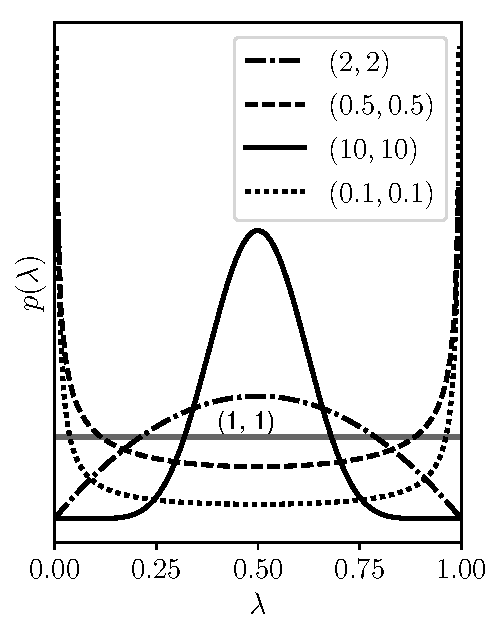
\includegraphics[width=0.99\linewidth]{Chapters/02_LinearAlgebra/30_prob/python/beta1.pdf}
\caption{$\alpha = \beta$}
\label{fig:30_3a}
\end{subfigure}
\begin{subfigure}{0.325\textwidth}
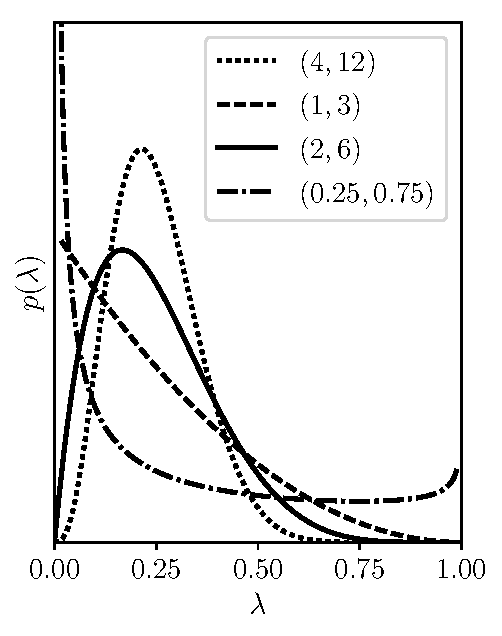
\includegraphics[width=0.99\linewidth]{Chapters/02_LinearAlgebra/30_prob/python/beta2.pdf}
\caption{$\alpha < \beta$}
\label{fig:30_3b}
\end{subfigure}
\begin{subfigure}{0.325\textwidth}
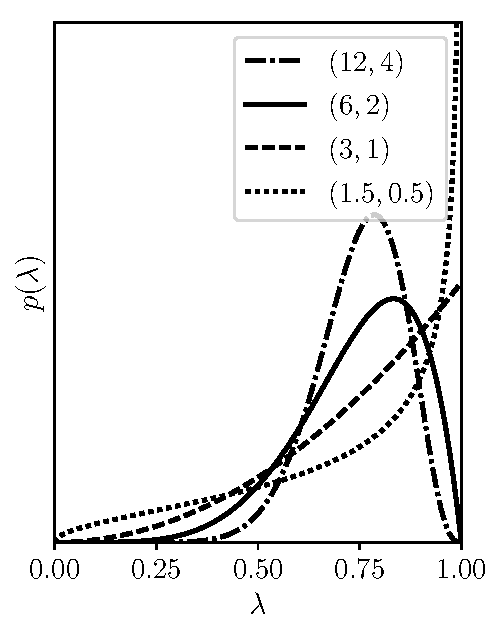
\includegraphics[width=0.99\linewidth]{Chapters/02_LinearAlgebra/30_prob/python/beta3.pdf}
\caption{$\alpha > \beta$}
\label{fig:30_3c}
\end{subfigure}
\caption{
Ví dụ về hàm mật độ xác suất của phân phối Beta. (a) $\alpha = \beta$, đồ thị
hàm số là đối xứng. (b) $\alpha < \beta$, đồ thị hàm số lệch sang trái, chứng tỏ xác suất $\lambda$ nhỏ là lớn. (c) $\alpha > \beta$, đồ thị hàm số lệch sang phải, chứng tỏ xác suất $\lambda$ lớn là lớn.
}
\label{fig:30_3}
\end{figure}
% ******************************************************************************

\begin{itemize}

\item Trong Hình \ref{fig:30_3a}, khi $\alpha =\beta$. Đồ thị của các hàm
mật độ xác suất đối xứng qua đường thẳng $\lambda = 0.5$. Khi $\alpha =
\beta = 1$, thay vào \eqref{eqn:30_34}, ta thấy $p(\lambda) = 1$ với mọi
$\lambda$. Trong trường hợp này, phân phối Beta trở thành \textit{phân phối
đều} Khi $\alpha = \beta > 1$, các hàm số đạt giá trị cao tại gần trung tâm,
tức $\lambda$ sẽ nhận giá trị xung quanh điểm 0.5 với xác suất cao. Khi
$\alpha = \beta < 1$, hàm số đạt giá trị cao tại các điểm gần 0 và 1.    % Điều này chứng tỏ Bernoulli distribution tương ứng với các $\lambda$ này
% bị thiên lệch nhiều.

\item Trong Hình~\ref{fig:30_3b}, khi $\alpha < \beta$, ta thấy rằng đồ thị
có xu hướng lệch sang bên trái. Các giá trị $(\alpha, \beta)$ này nên được
sử dụng nếu ta dự đoán rằng $\lambda$ là một số nhỏ hơn $0.5$.

\item Trong Hình~\ref{fig:30_3c}, khi $\alpha > \beta$, điều ngược lại xảy
ra với các hàm số đạt giá trị cao tại các điểm gần 1.
\end{itemize}


\subsection{Phân phối Dirichlet}
\index{phân phối xác suất -- probability distribution!phân phối Dirichlet}
\index{probability distribution -- phân phối xác suất!phân phối Dirichlet}

Phân phối Dirichlet chính là trường hợp tổng quát của phân phối Beta khi được
dùng để mô tả tham số của phân phối categorical. Nhắc lại rằng phân phối
categorical là trường hợp tổng quát của phân phối Bernoulli.

Phân phối Dirichlet được định nghĩa trên $K$ biến liên tục $\lambda_1, \dots,
\lambda_K$ trong đó các $\lambda_k$ không âm và có tổng bằng một. Bởi vậy, nó
phù hợp để mô tả tham số của phân phối categorical.
Có $K$ tham số {dương} để mô tả một phân phối Dirichlet:
$\alpha_1, \dots, \alpha_K$.

Hàm mật độ xác suất của phân phối Dirichlet được cho bởi
\begin{equation}
\label{eqn:30_35}
p(\lambda_1, \dots, \lambda_K) = \frac{\Gamma(\sum_{k=1}^K \alpha_k)}{\prod_{k=1}^K\Gamma(\alpha_k)} \prod_{k=1}^K \lambda_k^{\alpha_k - 1}.
\end{equation}
Dạng thu gọn của nó là
$p(\lambda_1, \dots, \lambda_K) = \text{Dir}_{\lambda_1, \dots, \lambda_K}[\alpha_1, \dots, \alpha_K]$.


% \section{Thảo luận }
% Về Xác suất thống kê, còn rất nhiều điều chúng ta cần lưu ý. Tạm thời, tôi ôn tập lại những kiến thức này để phục vụ cho một số bài viết tiếp theo. Khi nào có phần nào cần nhắc lại, tôi sẽ ôn tập thêm cho các bạn.



% \section{Tài liệu tham khảo }
% [1] Chương 2, 3 của \href{http://www.computervisionmodels.com}{Computer Vision:
% Models, Learning, and Inference}. Simon J.D. Prince.

%!TEX root = ../../book_ML.tex
\chapter{Ước lượng tham số mô hình}




\section{Giới thiệu}
% \textbf{Những sự kiện có xác suất cao là những sự kiện có khả năng xảy ra hơn.}

% Câu nói \textit{nói cũng như không này} là khơi nguồn cho rất nhiều các thuật toán Machine Learning có liên quan đến xác suất.

% Một mô hình machine learning thường bao gồm ba thành phần:
% \textbf{Modeling, Learning} và \textbf{Inference}\footnote{Xem Chương 6 của
% \href{http://www.computervisionmodels.com/}{Computer Vision: Models, Learning,
% and Inference}}.

% \textbf{Modeling là việc đi tìm môt mô hình thích hợp cho bài toán cần giải
% quyết.} Với bài toán linear regression, modeling chính là việc mô hình dữ liệu
% đầu ra như là tổ hợp tuyến tính của các đặc trưng. Với bài toán k-means
% clustering, modeling chính là việc quan sát ra rằng các clusters thường được mô
% tả bởi các \textit{centroids} và mỗi điểm được xếp vào cluster tương ứng với
% centroid gần nó nhất. Việc đi tìm ra mô hình nào phù hợp cho bài toán chính là
% bước \textbf{modeling}.

% \textbf{Learning là bước tiến hành tối ưu các tham số của mô hình.} Với linear
% regression, tham số mô hình là bộ vector hệ số và bias $(\mathbf{w}, b)$. Quá
% trình tối thiểu hoá hàm mất mát của nó chính là
% quá trình đi tìm tham số của mô hình, chính là quá trình \textbf{learning}.

% \textbf{Inference là bước dự đoán đầu của mô hình khi có đầu vào mới.} Với
% linear regression, inference chính là việc tính $y = \mathbf{w}^T\mathbf{x} + b$
% dựa trên bộ các tham số đã được huấn luyện $(\mathbf{w}, b)$. So với hai bước
% modeling và learning, inference thường đơn giản hơn.

% Với các mô hình xác Việc
% \textit{Inference} có thể coi

% Các mô hình machine learning thống kế (\textit{statistical machine learning})
% đóng vai trò
\index{uoc@ước lượng tham số -- parameter estimation}
\index{parameter estimation -- ước lượng tham số}
\index{tham số mô hình -- model parameter}
\index{model parameter -- tham số mô hình}
Có rất nhiều mô hình machine learning được xây dựng dựa trên các mô hình thống
kê. Các mô hình thống kê thường dựa trên các phân phối xác suất đã được đề cập
trong Chương~\ref{cha:prob}. Với một mô hình thông kê bất kỳ, ký hiệu $\theta$
là tập hợp tất cả các tham số của mô hình đó. Với phân phối Bernoulli, tham số
là biến $\lambda$. Với phân phối chuẩn nhiều chiều, các tham số là vector kỳ
vọng $\bmu$ và ma trận hiệp phương sai $\bSigma$.  ``Learning'' chính là quá
trình {ước lượng} bộ tham số $\theta$ sao cho mô hình tìm được khớp với phân
phối của dữ liệu nhất. Quá trình này còn được gọi là \textit{ước lượng tham số} (parameter estimation).

% \index{uoc@ước lượng hợp lý cực đại -- maximum likelihood estimation}
\index{uoc@ước lượng hậu nghiệm cực đại -- maximum a posteriori estimation}
\index{maximum a posteriori estimation -- ước lượng hậu nghiệm cực đại}
\index{MAP estimation}

Có hai cách ước lượng tham số thường được dùng trong các mô hình machine
learning thống kê. Cách thứ nhất chỉ dựa trên dữ liệu đã biết trong tập huấn
luyện, được gọi là \textit{ước lượng hợp lý cực đại}({maximum likelihood
estimation} hay {ML estimation} hoặc \textit{MLE}). Cách thứ hai không
những dựa trên tập huấn luyện mà còn dựa trên những thông tin biết trước của các
tham số. Những thông tin này có thể có được bằng {cảm quan} của người xây dựng
mô hình. {Cảm quan} càng rõ ràng, càng hợp lý thì khả năng thu được bộ tham số
tốt càng cao. Chẳng hạn, thông tin biết trước của $\lambda$ trong phân phối
Bernoulli là việc nó là một số trong đoạn $[0, 1]$. Với bài toán tung đồng xu,
với $\lambda$ là xác suất có được mặt xấp, ta dự đoán được rằng giá trị này là
một số gần với $0.5$. Cách ước lượng tham số thứ hai này được gọi là \textit{ước
lượng hậu nghiệm cực đại} ({maximum a posteriori estimation} hay
{MAP estimation}). Trong chương này, chúng ta cùng tìm hiểu ý tưởng và
cách giải quyết bài toán ước lượng tham số mô hình theo {MLE} hoặc {MAP}.


\section{Ước lượng hợp lý cực đại}
\index{uoc@ước lượng hợp lý cực đại -- maximum likelihood estimation}
\index{maximum likelihood estimation -- ước lượng hợp lý cực đại}
\index{MLE}
\subsection{Ý tưởng}
Giả sử có các điểm dữ liệu $\mathbf{x}_1, \mathbf{x}_2, \dots, \mathbf{x}_N$ tuân theo một phân phối nào đó được mô tả bởi bộ tham số $\theta$.
Ước lượng hợp lý cực đại là việc đi tìm bộ tham số $\theta$ để
\begin{equation}
\label{eqn:31_1}
\theta = \argmax_{\theta} p(\mathbf{x}_1, \dots, \mathbf{x}_N | \theta).
\end{equation}
Bài toán~\eqref{eqn:31_1} có ý nghĩa như thế nào và vì sao việc này hợp lý?

\index{hàm hợp lý -- likelihood}
\index{likelihood -- hàm hợp lý}
Giả sử rằng ta đã biết rằng mô hình có dạng đặc biệt được mô tả bởi bộ tham số
$\theta$. Xác suất có điều kiện $p(\mathbf{x}_1 | \theta)$ chính là xác suất xảy
ra {sự kiện} $\mathbf{x}_1$ trong trường hợp mô hình được mô tả bởi bộ tham số
$\theta$. Tương tự, $p(\mathbf{x}_1, \dots, \mathbf{x}_N | \theta)$ là xác suất
để toàn bộ các {sự kiện} $\mathbf{x}_1, \mathbf{x}_2, \dots, \mathbf{x}_N$ đồng
thời xảy ra, xác suất đồng thời này còn được gọi là \textit{sự hợp lý} ({likelihood}).

Phân phối của dữ liệu và bản thân dữ liệu có thể lần lượt được coi là nguyên nhân và kết quả. Ta cần tìm nguyên nhân (bộ tham số $\theta$) để khả năng xảy ra kết quả (hàm hợp lý) là cao nhất.


\subsection{Giả sử về sự độc lập và log-likelihood}
\index{log-likelihood}
Người ta thường ít khi giải trực tiếp bài toán~\eqref{eqn:31_1} vì khó tìm được
một mô hình xác suất đồng thời cho toàn bộ dữ liệu. Một cách tiếp cận phổ biến là đơn giản hoá mô hình bằng cách giả sử các điểm dữ liệu $\mathbf{x}_n$
độc lập với nhau khi biết bộ tham số $\theta$. Nói cách khác, hàm hợp lý trong~\eqref{eqn:31_1} được xấp xỉ
bởi\footnote{Nhắc lại rằng nếu hai sự kiện $x, y$ là độc lập thì xác suất đồng thời bằng tích xác suất của từng sự kiện: $p(x, y) = p(x)p(y)$. Với
xác suất có điều kiện, $p(x, y | z) = p(x|z)p(y|z)$.}
\begin{equation}
\label{eqn:31_2}
p(\mathbf{x}_1, \dots, \mathbf{x}_N | \theta) \approx \prod_{n = 1}^N p(\mathbf{x}_n |\theta).
\end{equation}
Lúc đó, bài toán~\eqref{eqn:31_1}
có thể được giải quyết bằng cách giải bài toán tối ưu
\begin{equation}
\label{eqn:31_3}
\theta = \argmax_{\theta} \prod_{n=1}^N p(\mathbf{x}_n| \theta)
\end{equation}
Mỗi giá trị $p(\bx_n |\theta)$ là một số dương nhỏ hơn một. Khi $N$ lớn, tích của các số dương này rất gần với 0, máy tính có thể không lưu chính xác được do sai số tính toán. Để tránh hiện tượng này, việc tối đa hàm mục tiêu thường được chuyển về việc tối đa logarit\footnote{Logarit là một hàm đồng biến.} của hàm mục tiêu:
\begin{equation}
\label{eqn:31_4}
\theta = \argmax_{\theta} \log\left(\prod_{n=1}^N p(\mathbf{x}_n| \theta)\right) = \argmax_{\theta} \sum_{n = 1}^N \log\left(p(\mathbf{x}_n | \theta)
\right).
\end{equation}

% \end{itemize}

% Chúng ta cùng xem vài ví dụ.


\subsection{Ví dụ}

\subsubsection{Ví dụ 1: Phân phối Bernoulli}
\textbf{Bài toán}: Giả sử tung một đồng xu $N$ lần và nhận được $n$ mặt
ngửa, hãy ước lượng xác suất nhận được mặt ngửa khi tung đồng xu đó.

\textit{\textbf{Lời giải:}}

Một cách tự nhiên, ta có thể ước lượng xác suất đó là $\lambda
= \frac{n}{N}$. Chúng ta cùng ước lượng giá trị này bằng phương pháp MLE.

Đặt $\lambda$ là xác suất để nhận được một mặt ngửa và $x_1, x_2,
\dots, x_N$ là các đầu ra quan sát thấy. Trong $N$ giá trị này, có $n$ giá trị bằng 1 tương ứng
với mặt ngửa và $m = N - n$ giá trị bằng 0 tương ứng với mặt
xấp. Nhận thấy
\begin{equation}
\sum_{i=1}^N x_i = n, ~~N - \sum_{i=1}^N x_i = N - n = m.
\end{equation}
Vì đây là một xác suất của biến ngẫu nhiên nhị phân rời rạc, sự kiện nhận được mặt ngửa hay xấp khi tung đồng xu tuân theo
phân phối Bernoulli:
\begin{equation}
p(x_i | \lambda) = \lambda^{x_i} ( 1- \lambda)^{1 - x_i}.
\end{equation}
Khi đó tham số mô hình $\lambda$ có thể được ước lượng bằng việc giải bài toán
tối ưu sau đây, với giả sử rằng kết quả của các lần tung đồng xu độc lập với
nhau:
% \begin{equation}
\begin{alignat}{3}
\lambda & =  \argmax_{\lambda}\left[ p(x_1, x_2, \dots, x_N | \lambda)\right]
% \label{eqn:31_5}
&& =  \argmax_{\lambda} \left[\prod_{i = 1}^N p(x_i | \lambda)\right] \\
\label{eqn:31_6}
& =  \argmax_{\lambda} \left[\prod_{i=1}^N  \lambda^{x_i} ( 1- \lambda)^{1 - x_i}\right]
% \label{eqn:31_7}
&& = \argmax_{\lambda} \left[\lambda^{\sum_{i=1}^N x_i} (1 - \lambda)^{N - \sum_{i=1}^N x_i}\right]  \\\
\label{eqn:31_8}
& = \argmax_{\lambda} \left[\lambda^{n} (1 - \lambda)^{m}\right]
% \label{eqn:31_9}
&& = \argmax_{\lambda} \left[ n\log(\lambda) + m\log(1 - \lambda) \right]
\end{alignat}
% \end{equation}
Tới đây, bài toán tối ưu~\eqref{eqn:31_8} có thể được giải bằng cách giải phương
trình đạo hàm của hàm mục tiêu bằng 0. Tức $\lambda$ là nghiệm của phương trình
\begin{eqnarray}
\label{eqn:31_10_new}
\frac{n}{\lambda} - \frac{m}{1 - \lambda}  =  0
\Leftrightarrow \frac{n}{\lambda}  =  \frac{m}{1 - \lambda}
\Leftrightarrow \lambda  =  \frac{n}{n + m} = \frac{n}{N}
\end{eqnarray}
% \end{equation}

Vậy kết quả ước lượng ban đầu là có cơ sở.


\subsubsection{Ví dụ 2: Phân phối categorical}
% Một ví dụ khác phức tạp hơn một chút.

\textbf{Bài toán:} Giả sử tung một viên xúc xắc sáu mặt có xác suất rơi vào các
mặt không đều nhau. Giả sử trong $N$ lần tung, số lượng xuất hiện các mặt
thứ nhất, thứ hai,\dots, thứ sáu lần lượt là $n_1, n_2, \dots, n_6$ lần với
$\displaystyle \sum_{i=1}^6 n_i = N$. Tính xác suất rơi vào mỗi mặt. Giả sử thêm rằng $n_i > 0, ~\forall i = 1, \dots, 6.$

\lg

Bài toán này phức tạp hơn bài toán trên, nhưng ta cũng có thể dự
đoán được ước lượng tốt nhất của xác suất rơi vào mặt thứ $i$ là $\lambda_i =
\frac{n_i}{N}$.

{Mã hoá} mỗi kết quả đầu ra thứ $i$ bởi một vector 6 chiều $\mathbf{x}_i
\in \{0, 1\}^6$ trong đó các phần tử của nó bằng 0 trừ phần tử tương ứng với mặt
quan sát được bằng 1. Ta có
$\sum_{i=1}^N x^j_i = n_j, ~ \forall j = 1, 2, \dots, 6$,
trong đó $x^j_i$ là thành phần thứ $j$ của vector $\mathbf{x}_i$.

Nhận thấy rằng xác suất rơi vào mỗi mặt tuân theo phân phối categorical với
các tham số $\lambda_j > 0, j = 1, 2, \dots, 6$. Ta dùng $\blambda$ để thể hiện
cho cả sáu tham số này.

Với các tham số $\blambda$, xác suất để sự kiện $\mathbf{x}_i$ xảy ra là
\begin{eqnarray}
p(\mathbf{x}_i | \blambda) = \prod_{j = 1}^6 \lambda_j^{x_i^j}
\end{eqnarray}
% \end{equation}
Khi đó, vẫn với giả sử về sự độc lập giữa các lần tung xúc xắc, ước lượng bộ
tham số $\lambda$ dựa trên việc tối đa log-likelihood ta có:
\begin{align}
% \lambda & = & \argmax_{\lambda} \left[ p(\mathbf{x}_1, \dots, \mathbf{x}_N  \| \lambda) \right]\\\
\label{eqn:31_10}
\blambda & =  \argmax_{\blambda} \left[ \prod_{i=1}^N p(\mathbf{x}_i |
\blambda) \right]
% \label{eqn:31_11}
=  \argmax_{\blambda} \left[ \prod_{i=1}^N  \prod_{j = 1}^6 \lambda_j^{x_i^j} \right]  \\\
\label{eqn:31_12}
& =  \argmax_{\blambda} \left[  \prod_{j = 1}^6 \lambda_j^{\sum_{i=1}^N x_i^j} \right]
=  \argmax_{\blambda} \left[  \prod_{j = 1}^6 \lambda_j^{n_j} \right]  \\\
\label{eqn:31_14}
& =  \argmax_{\blambda} \left[  \sum_{j=1}^6 n_j\log(\lambda_j) \right].
\end{align}
% \end{equation}
Khác với bài toán~\eqref{eqn:31_8}, chúng ta không được quên điều kiện
$\sum_{j=1}^6 \lambda_j = 1$. Ta có bài toán tối ưu có ràng buộc sau đây:
\begin{equation}
\label{eqn:31_15}
\begin{aligned}
\max_{\lambda}  \sum_{j=1}^6 n_j\log(\lambda_j) \quad
\text{thoả mãn:}  \sum_{j=1}^6 \lambda_j = 1
\end{aligned}
\end{equation}
Bài toán tối ưu này có thể được giải bằng phương pháp nhân tử Lagrange (xem Phụ
lục~\ref{apd:lagrange}).

Lagrangian của bài toán này là
\begin{equation}
\mathcal{L}(\lambda, \mu) = \sum_{j=1}^6 n_j\log(\lambda_j) + \mu (1- \sum_{j=1}^6 \lambda_j)
\end{equation}
Nghiệm của bài toán là nghiệm của hệ đạo hàm $\mathcal{L}(.)$ theo từng biến bằng 0:
\begin{alignat}{3}
\label{eqn:31_16}
\frac{\partial \mathcal{L}(\lambda, \mu)}{\partial \lambda_j} &=   \frac{n_j}{\lambda_j} - \mu &&=  0,~ \forall j = 1, 2, \dots, 6;\\
\label{eqn:31_17}
\frac{\partial \mathcal{L}(\lambda, \mu)}{\partial \mu} &=  1-\sum_{j=1}^6 \lambda_j &&= 0.
\end{alignat}
Từ~\eqref{eqn:31_16} ta có $\lambda_j = \frac{n_j}{\mu}$. Thay
vào~\eqref{eqn:31_17}:
\begin{equation}
\sum_{j=1}^6 \frac{n_j}{\mu} = 1 \Rightarrow \mu = \sum_{j=1}^6 n_j = N
\end{equation}
Từ đó ta có ước lượng
% \begin{equation}
$\lambda_j = \frac{n_j}{N}, ~~\forall j = 1, 2, \dots, 6$.
% \end{equation}

Qua hai ví dụ trên ta thấy MLE cho kết quả khá hợp lý.


\subsubsection{Ví dụ 3: Phân phối chuẩn một chiều}
\label{sssec:gassian_mle}

\textbf{Bài toán:} Khi thực hiện một phép đo, giả sử rằng rất khó để có thể đo
{chính xác} độ dài của một vật. Thay vào đó, người ta thường đo vật đó
nhiều lần rồi suy ra kết quả, với giả thiết rằng các phép đo độc lập với nhau
và kết quả mỗi phép đo tuân theo một phân phối chuẩn. Hãy ước lượng chiều dài của vật đó
dựa trên các kết quả đo được.

\lg

Vì đã biết kết quả phép đo tuân theo phân phối chuẩn, ta sẽ đi tìm phân phối
chuẩn đó. Chiều dài của vật có thể được coi là giá trị mà hàm mật độ xác suất
đạt giá trị cao nhất. Trong phân phối chuẩn, ta biết rằng hàm mật độ xác suất
đạt giá trị lớn nhất tại kỳ vọng của phân phối đó. Chú ý rằng kỳ vọng của phân
phối và kỳ vọng của dữ liệu quan sát được có thể không bằng nhau, nhưng rất gần
nhau. Nếu ước lượng kỳ vọng của phân phối bằng MLE, ta sẽ thấy rằng kỳ vọng của
dữ liệu chính là đánh giá tốt nhất cho kỳ vọng của phân phối.

Thật vậy, giả sử các kích thước quan sát được là $x_1, x_2, \dots, x_N$. Ta cần
đi tìm một phân phối chuẩn, được mô tả bởi giá trị kỳ vọng $\mu$ và phương
sai $\sigma^2$, sao cho các giá trị $x_1, x_2, \dots, x_N$ là hợp lý nhất. Ta đã biết rằng, hàm mật độ xác suất tại $x_i$ của môt phân phối chuẩn có
kỳ vọng $\mu$ và phương sai $\sigma^2$ là
\begin{equation}
p(x_i | \mu, \sigma^2) = \frac{1}{\sqrt{2\pi \sigma^2}} \exp\left(-\frac{(x_i - \mu)^2}{2\sigma^2}\right).
\end{equation}
Để đánh giá $\mu$ và $\sigma$, ta sử dụng MLE với giả thiết rằng kết quả
các phép đo là độc lập:
\begin{alignat}{3}
\label{eqn:31_18}
\mu, \sigma & =
\argmax_{\mu, \sigma} \left[ \prod_{i=1}^N p(x_i | \mu,
\sigma^2)\right]\\\
\label{eqn:31_19}
& =  \argmax_{\mu, \sigma} \left[ \frac{1}{(2\pi \sigma^2)^{N/2}} \exp\left(-\frac{\sum_{i=1}^N (x_i - \mu)^2}{2\sigma^2} \right) \right]\\\
\label{eqn:31_20}
& =  \argmax_{\mu, \sigma}\left[ -N\log(\sigma) - \frac{\sum_{i=1}^N (x_i - \mu)^2}{2\sigma^2} \triangleq J(\mu, \sigma) \right].
\end{alignat}
Ta đã lấy logarit của hàm bên trong dấu ngoặc vuông của~\eqref{eqn:31_19} để
được~\eqref{eqn:31_20}, phần hằng số có chứa $2\pi$ cũng đã được bỏ đi vì
không ảnh hưởng tới kết quả.

Để tìm $\mu$ và $\sigma$, ta giải hệ phương trình đạo hàm của
$J(\mu, \sigma)$ theo mỗi biến bằng không:
\begin{alignat}{3}
\label{eqn:31_21}
\frac{\partial J}{\partial \mu} & = \frac{1}{\sigma^2}\sum_{i=1}^N(x_i - \mu) = 0 \\
\label{eqn:31_22}
\frac{\partial J}{\partial \sigma} & =  -\frac{N}{\sigma} + \frac{1}{\sigma^3}
\sum_{i=1}^N (x_i - \mu)^2  = 0 \\
% \begin{equation}
\imply
\mu  &=  \frac{\sum_{i=1}^N x_i}{N}, \quad
\sigma^2  =  \frac{\sum_{i=1}^N (x_i - \mu)^2}{N}.
% \end{equation}
\end{alignat}

Kết quả thu được không có gì bất ngờ.


\subsubsection{Ví dụ 4: Phân phối chuẩn nhiều chiều}
\textbf{Bài toán:} Giả sử tập dữ liệu ta thu được là các giá trị nhiều chiều
$\mathbf{x}_1, \dots, \mathbf{x}_N$ tuân theo phân phối chuẩn. Hãy đánh giá
vector kỳ vọng $\bmu$ và ma trận hiệp phương sai $\bSigma$ của phân phối này bằng MLE, giả sử rằng các $\mathbf{x}_1, \dots, \mathbf{x}_N$ độc lập.

\lg

Việc chứng minh các công thức
\begin{eqnarray}
\bmu & = & \frac{\sum_{i=1}^N \mathbf{x}_i}{N}, \\\
\bSigma & = & \frac{1}{N}\sum_{i=1}^N (\mathbf{x} - \mu)(\mathbf{x} - \mu)^T
\end{eqnarray}
xin được dành lại cho bạn đọc như một bài tập nhỏ. Dưới đây là một vài gợi ý:

\begin{itemize}
\item Hàm mật độ xác suất của phân phối chuẩn nhiều chiều là
\begin{equation}
p(\mathbf{x} | \bmu, \bSigma) = \frac{1}{(2\pi)^{D/2} |\bSigma|^{1/2}} \exp \left(-\frac{1}{2} (\mathbf{x} - \bmu)^T \bSigma^{-1} (\mathbf{x} - \bmu)\right).
\end{equation}
Chú ý rằng ma trận hiệp phương sai $\bSigma$ là xác định dương nên có nghịch đảo.
\item Một vài đạo hàm theo ma trận:
\begin{align}
\nabla_{\bSigma} \log |\bSigma| &= (\bSigma^{-1})^T \triangleq
\bSigma^{-T}~~~ \text{(chuyển vị của nghịch đảo)}\\
\nabla_{\bSigma} (\mathbf{x}_i - \bmu)^T \bSigma^{-1} (\mathbf{x}_i-\bmu) &= -\bSigma^{-T}(\mathbf{x}_i - \bmu)(\mathbf{x}_i - \bmu)^T\bSigma^{-T}
\end{align}
\end{itemize}
(Xem thêm \textit{Matrix Calculus}, mục D.2.1 và D.2.4 tại
\url{https://goo.gl/JKg631}.)


\section{Ước lượng hậu nghiệm cực đại}
\index{uoc@ước lượng hậu nghiệm cực đại -- maximum a posteriori estimation, MAP estimation}
\index{maximum a posteriori estimation, MAP estimation -- ước lượng hậu nghiệm cực đại}
\index{MAP}
\subsection{Ý tưởng}
Quay lại với Ví dụ 1 về bài toán tung đồng xu. Nếu tung đồng xu 5000 lần và nhận
được 1000 lần ngửa, ta có thể đánh giá xác suất nhận được mặt ngửa là $1/5$ và
việc đánh giá này là đáng tin vì số mẫu lớn. Nếu tung năm lần và chỉ nhận được
một mặt ngửa, theo MLE, xác suất để có một mặt ngửa được ước lượng là $1/5$. Tuy
nhiên với chỉ năm kết quả, ước lượng này là không đáng tin. Khi tập huấn luyện
quá nhỏ, ta cần quan tâm thêm tới một vài giả thiết của các tham số. Trong
ví dụ này, một giả thiết hợp lý là xác suất nhận được mặt ngửa gần với $1/2$.

\textit{Ước lượng hậu nghiệm cực đại} (maximum a posteriori, MAP) ra
đời nhằm giải quyết vấn đề này. Trong MAP, ta giới thiệu một giả thiết biết
trước của tham số $\theta$. Từ giả thiết này, ta có thể
suy ra các khoảng giá trị và phân bố của tham số.

\index{xác suất hậu nghiệm -- posterior probability}
\index{posterior probability -- xác suất hậu nghiệm}
Khác với MLE, trong MAP, ta đánh giá tham số như một xác suất có
điều kiện của dữ liệu:
\begin{equation}
\label{eqn:31_34}
\theta = \argmax_{\theta} \underbrace{p(\theta | \mathbf{x}_1, \dots, \mathbf{x}_N)}_{\text{hậu nghiệm}}.
\end{equation}
Biểu thức $p(\theta | \mathbf{x}_1, \dots, \mathbf{x}_N) $ còn được gọi là
{xác suất hậu nghiệm} của $\theta$. Chính vì vậy, việc ước lượng
$\theta$ theo~\eqref{eqn:31_34} được gọi là ước lượng hậu nghiệm cực đại.

Thông thường, hàm tối ưu trong~\eqref{eqn:31_34} khó xác định dạng một cách trực
tiếp. Chúng ta thường biết điều ngược lại, tức nếu biết tham số, ta có thể tính
được hàm mật độ xác suất của dữ liệu. Vì vậy, để giải bài toán MAP, quy tắc Bayes thường được sử dụng. Bài toán MAP được biến đổi thành
\begin{align}
\label{eqn:31_35}
\theta & =  \argmax_{\theta} p(\theta | \mathbf{x}_1, \dots, \mathbf{x}_N)
=  \argmax_{\theta} \left[ \frac{\overbrace{p(\mathbf{x}_1, \dots,
\mathbf{x}_N | \theta)}^{\text{hàm hợp lý}}
\overbrace{p(\theta)}^{\text{tiên nghiệm}}}{p(\mathbf{x}_1, \dots, \mathbf{x}_N)} \right] \\
\label{eqn:31_36}
& =  \argmax_{\theta} \left[ p(\mathbf{x}_1, \dots, \mathbf{x}_N | \theta)
p(\theta) \right] \\
\label{eqn:31_37}
& =  \argmax_{\theta} \left[ \prod_{i=1}^N p(\mathbf{x}_i | \theta) p(\theta) \right].
\end{align}

Đẳng thức~\eqref{eqn:31_35} xảy ra theo quy tắc Bayes. Đẳng
thức~\eqref{eqn:31_36} xảy ra vì mẫu số của~\eqref{eqn:31_35} không phụ thuộc vào
tham số $\theta$. Đẳng thức~\eqref{eqn:31_37} xảy ra nếu có giả thiết về
sự độc lập giữa các $\mathbf{x}_i$.

\index{tiên nghiệm -- prior}
\index{prior -- tiên nghiệm}

Như vậy, điểm khác biệt lớn nhất giữa hai bài toán tối ưu MLE và MAP là việc hàm
mục tiêu của MAP có thêm $p(\theta)$, tức phân phối của $\theta$. Phân phối này
chính là những thông tin biết trước về $\theta$ và được gọi là
\textit{tiên nghiệm} (prior). Ta kết luận rằng hậu nghiệm tỉ lệ thuận với
tích của hàm hợp lý và tiên nghiệm.


Để chọn tiên nghiệm chúng ta cùng làm quen với một khái
niệm mới: \textit{tiên nghiệm liên hợp} (conjugate prior).


\subsection{Tiên nghiệm liên hợp}
\index{tiên nghiệm liên hợp -- conjugate prior}
\index{conjugate prior -- tiên nghiệm liên hợp}
\index{phân phối liên hợp -- conjugate distribution}
\index{conjugate distribution -- phân phối liên hợp}
Nếu phân phối hậu nghiệm $p(\theta | \mathbf{x}_1, \dots,
\mathbf{x}_N)$ có cùng dạng với phân phối tiên nghiệm $p(\theta)$, hai phân phối này được gọi là cặp \textit{phân phối liên hợp} (conjugate distribution), và $p(\theta)$ được
gọi là \textit{tiên nghiệm liên hợp} của hàm hợp lý $p(\mathbf{x}_1, \dots,
\mathbf{x}_N | \theta)$. Ta sẽ thấy rằng bài toán MAP và MLE có cấu trúc giống nhau.
% Nếu \textit{posterior distribution} $p(\theta \| \mathbf{X})$ và \textit{likelihood} $p(\mathbf{X} \|\theta)$ có cùng \textit{họ} (family), thì \textit{prior distribution} là \textit{conjugate distribution} của \textit{likelihood distribution}.

% Tôi sẽ không đi sâu vào phần này, bạn đọc có thể đọc thêm \href{https://en.wikipedia.org/wiki/Conjugate_prior}{Conjugate prior}.

Một vài cặp phân phối liên hợp\footnote{Đọc thêm:
\textit{Conjugate prior -- Wikipedia} (\url{https://goo.gl/E2SHbD}).}:

\begin{itemize}
\item Nếu hàm hợp lý và tiên nghiệm cho vector kỳ vọng là các phân phối
chuẩn thì phân phối hậu nghiệm cũng là một phân phối chuẩn. Ta nói rằng phân
phối chuẩn liên hợp với chính nó, hay còn gọi là \textit{tự liên hợp} (self-conjugate).

\item Nếu hàm hợp lý là một phân phối chuẩn và tiên nghiệm
cho phương sai là một {phân phối gamma}, phân phối hậu nghiệm cũng là một phân phối chuẩn. Ta nói rằng phân phối gamma là tiên nghiệm liên hợp cho phương sai của phân phối chuẩn.

\item Phân phối beta là liên hợp của phân phối Bernoulli.

\item Phân phối Dirichlet là liên hợp của phân phối categorical.

\end{itemize}

\subsection{Siêu tham số}
Xét phân phối Bernoulli với hàm mật độ xác suất
\begin{equation}
p(x | \lambda) = \lambda^x ( 1 - \lambda)^{1 - x}
\end{equation}
và liên hợp của nó, phân phối beta, có hàm phân mật độ xác suất
\begin{equation}
p(\lambda) = \frac{\Gamma(\alpha + \beta)}{\Gamma(\alpha) \Gamma(\beta)} \lambda^{\alpha - 1} ( 1 - \lambda) ^{\beta - 1}.
\end{equation}
Bỏ qua thành phần hằng số chỉ mang mục đích chuẩn hoá, ta có thể nhận thấy rằng
phần còn lại của phân phối beta có cùng dạng với phân phối Bernoulli. Cụ thể,
nếu sử dụng phân phối beta làm tiên nghiệm cho tham số $\lambda$, và bỏ qua
phần thừa số hằng số, hậu nghiệm sẽ có dạng
\begin{eqnarray}
\nonumber
p(\lambda | x) & \propto & p(x | \lambda) p(\lambda) \\\
\label{eqn:31_38}
& \propto & \lambda^{x + \alpha - 1}(1 - \lambda)^{1 - x + \beta - 1}
\end{eqnarray}
Nhận thấy~\eqref{eqn:31_38} {vẫn có dạng của một phân phối
Bernoulli.} Vì vậy, phân phối beta là một tiên nghiệm liên hợp của phân phối Bernoulli.

\index{siêu tham số -- hyperparameter}
\index{hyperparameter -- siêu tham số}
Trong ví dụ này, tham số $\lambda$ phụ thuộc vào hai tham số khác là $\alpha$ và
$\beta$. Để tránh nhầm lẫn, hai tham số $(\alpha, \beta)$ được gọi là các
\textit{siêu tham số} (hyperparameter).

Quay trở lại ví dụ về bài toán tung đồng xu $N$ lần có $n$ lần nhận được mặt
ngửa và $m = N - n$ lần nhận được mặt xấp. Nếu sử dụng MLE,
ta nhận được ước lượng $\lambda = n/M$. Nếu sử dụng MAP với tiên nghiệm là một
$\text{beta}[\alpha, \beta]$ thì kết quả sẽ thay đổi thế nào?

Bài toán tối ưu MAP
\begin{eqnarray}
\nonumber
\lambda & = & \argmax_{\lambda} \left[p(x_1, \dots, x_N | \lambda) p(\lambda) \right] \\\
\nonumber
& = & \argmax_{\lambda} \left[\left(\prod_{i=1}^N \lambda^{x_i} ( 1- \lambda)^{1 - x_i}\right) \lambda^{\alpha - 1} ( 1 - \lambda)^{\beta - 1} \right] \\\
\nonumber
& = & \argmax_{\lambda} \left[ \lambda^{\sum_{i = 1}^N x_i + \alpha - 1} ( 1- \lambda)^{N - \sum_{i=1}^N x_i + \beta - 1} \right] \\\
\label{eqn:31_39}
& = & \argmax_{\lambda} \left[ \lambda^{n + \alpha - 1} ( 1- \lambda)^{m + \beta - 1} \right]
\end{eqnarray}
Bài toán tối ưu~\eqref{eqn:31_39} chính là bài toán tối ưu~\eqref{eqn:31_8} với
tham số thay đổi một chút. Tương tự như~\eqref{eqn:31_10_new}, nghiệm
của~\eqref{eqn:31_39} là
\begin{equation}
\label{eqn:31_40}
\lambda = \frac{n + \alpha - 1}{n + m + \alpha + \beta - 2}= \frac{n + \alpha - 1}{N + \alpha + \beta - 2}
\end{equation}
Việc chọn tiên nghiệm phù hợp đã khiến cho việc tối ưu bài toán MAP được thuận
lợi.


Việc còn lại là chọn cặp siêu tham số $\alpha$ và $\beta$.

Chúng ta cùng xem lại dạng của phân phối beta và thấy rằng khi $\alpha
= \beta > 1$, hàm mật độ xác suất của phân phối beta đối xứng qua điểm 0.5 và
đạt giá trị cao nhất tại 0.5. Xét Hình~\ref{fig:31_1}, ta thấy rằng khi
$\alpha =\beta > 1$, mật độ xác suất xung quanh điểm 0.5 nhận giá trị
cao, điều này chứng tỏ $\lambda$ có xu hướng gần 0.5.

Nếu chọn $\alpha = \beta = 1$, ta nhận được phân phối đều vì đồ thị hàm mật
độ xác suất là một đường thẳng. Lúc này, xác suất của $\lambda$ tại mọi vị trí
trong khoảng $[0, 1]$ là như nhau. Thực chất, nếu ta thay $\alpha = \beta = 1$
vào~\eqref{eqn:31_40} ta sẽ thu được $\lambda = n/N$, đây chính là ước lượng thu
được bằng MLE. MLE là một trường hợp đặc biệt của MAP khi prior là một phân phối
đều.

\begin{figure}[t]
% caption on side
\floatbox[{\capbeside\thisfloatsetup{capbesideposition={right,top},capbesidewidth=6cm}}]{figure}[\FBwidth]
{\caption{ Đồ thị hàm mật độ xác suất của phân phối beta khi $\alpha =
\beta$ và nhận các giá trị khác nhau. Khi cả hai giá trị này lớn, xác suất
để $\lambda$ gần 0.5 sẽ cao hơn. }
\label{fig:31_1}}
{ % figure here
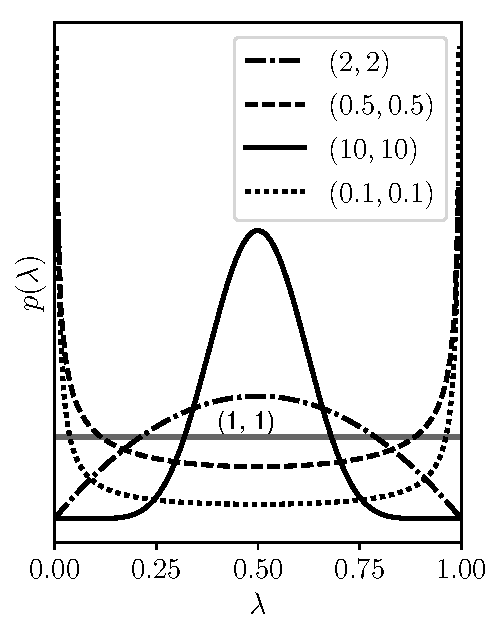
\includegraphics[width=.45\textwidth]{Chapters/02_LinearAlgebra/30_prob/python/beta1.pdf}
}
\end{figure}


% <hr>
% <div>
% <table width = "100%" style = "border: 0px solid white">
%     <tr >
%         <td height="100%" style = "border: 0px solid white" align = "center">
%         <img style="display:block;" width = "100%" src = "/assets/30_prob/beta1.png">
%          <br>

%          </td>
%          <td width="40%" style = "border: 0px solid white" align = "justify">
%          Hình 1: Đồ thị hàm mật độ xác suất của phân phối beta khi $\alpha = \beta$ và nhận các giá trị khác nhau. Khi cả hai giá trị này lớn, xác suất để $\lambda$ gần 0.5 sẽ cao hơn.
%          </td>
%     </tr>
% </table>
% </div>


Nếu ta chọn $\alpha = \beta = 2$, ta sẽ thu được:
\begin{math} \displaystyle
\lambda= \frac{n + 1}{N + 2}
\end{math}.
Chẳng hạn khi $N = 5, n = 1$ như trong ví dụ. MLE cho kết quả $\lambda = 1/5$,
MAP sẽ cho kết quả $\lambda = 2/7$, gần với $1/2$ hơn.

Nếu chọn $\alpha = \beta = 10$ ta sẽ có $\lambda = (1 + 9)/(5 + 18) = 10/23$. Ta
thấy rằng khi $\alpha = \beta$ và càng lớn thì ta sẽ thu được $\lambda$ càng gần
$1/2$. Điều này có thể dễ nhận thấy vì prior nhận giá trị rất cao tại 0.5 khi
các siêu tham số $\alpha = \beta$ lớn.


% \subsection{MAP giúp tránh overfitting}
% Các siêu tham số thường được chọn dựa trên thực nghiệm, chẳng hạn bằng
% phương pháp hợp thức chéo. Việc thử nhiều bộ tham số rồi chọn ra bộ tốt nhất là việc mà
% các kỹ sư machine learning thường xuyên phải đối mặt. Cũng giống như việc chọn
% regularization parameter để tránh overfitting vậy.

% % Rõ ràng MAP cho chúng ta các kết quả \textit{linh hoạt} (flexible) với sự thay
% % đổi của hyperparameters. Và là một cách để tránh
% % \href{http://machinelearningcoban.com/2017/03/04/overfitting/}{overfitting}.

% Nếu viết lại bài toán MAP dưới dạng:
% \begin{eqnarray}
%   \theta & = & \argmax_{\theta} p(\mathbf{X}| \theta) p(\theta) \\\
%   & = & \argmax_{\lambda} \left[ \log \underbrace{p(\mathbf{X}| \theta)}_{\text{likelihood}} + \log \underbrace{p(\theta)}_{\text{prior}} \right]
% \end{eqnarray}
% ta có thể thấy rằng hàm mục tiêu có dạng $\L(\theta) + \lambda R(\theta)$ giống
% như trong regularization, với hàm log-likelihood đóng vai trò như hàm mất mát
% $\L(\theta)$, và log của prior đóng vai trò như hàm $R(\theta)$. Ta có thể nói
% rằng, MAP chính là một phương pháp giúp tránh overfitting trong các mô hình
% machine learning thống kê. MAP đặc biệt hữu ích khi tập huấn luyện là nhỏ.



\section{Tóm tắt}
\begin{itemize}
\item Khi sử dụng các mô hình thống kê machine learning, chúng ta thường
xuyên phải ước lượng các tham số của mô hình $\theta$. Có hai phương pháp phổ biến được sử dụng để
ước lượng $\theta$ là ước lượng hợp lý cực đại (MLE) và ước lượng hậu nghiệ cực đại (MAP).

\item Với MLE, việc xác định tham số $\theta$ được thực hiện bằng cách đi
tìm các tham số sao cho xác suất của tập huấn luyện, được xác định bằng
hàm {hợp lý}, là lớn nhất:
\begin{equation}
\theta = \argmax_{\theta} p(\mathbf{x}_1, \dots, \mathbf{x}_N |\theta).
\end{equation}

\item Để giải bài toán tối ưu này, giả thiết các dữ liệu $\mathbf{x}_i$ độc lập thường được sử dụng. Và bài toán MLE trở thành
\begin{equation}
\theta = \argmax_{\theta} \prod_{i=1}^N p(\mathbf{x}_i | \theta).
\end{equation}

\item Với MAP, các tham số được đánh giá bằng cách tối đa {hậu nghiệm}:
\begin{equation}
\theta = \argmax_{\theta} p(\theta | \mathbf{x}_1, \dots, \mathbf{x}_N)
\end{equation}
\item Quy tắc Bayes và giả thiết về sự độc lập của dữ
liệu thường được sử dụng:
\begin{equation} \theta = \argmax_{\theta}
\left[\prod_{i=1}^N p(\mathbf{x}_i | \theta) p(\theta) \right]
\end{equation}
Hàm mục tiêu ở đây chính là tích của {hàm hợp lý} và tiên nghiệm.


\item Tiên nghiệm thường được chọn dựa trên các thông tin biết trước của
tham số, và phân phối được chọn thường là các phân phối liên hợp của likelihood.

\item MAP có thể được coi như một phương pháp giúp tránh thiên lệch khi có
ít dữ liệu huấn luyện.

\end{itemize}


% \section{Đọc thêm}
% \begin{enumerate}
%     \item Chapter 4, 6 của \href{http://www.computervisionmodels.com}{Computer Vision:  Models, Learning, and Inference - Simon J.D. Prince.}

%     \item \href{https://en.wikipedia.org/wiki/Conjugate_prior}{Conjugate prior
%      --  Wikipedia.}

% \end{enumerate}


\setcounter{part}{1}
\setcounter{chapter}{4}
%!TEX root = ..//book_ML.tex
\part{Tổng quan}
\label{part:overview}

%!TEX root = ../../book_ML.tex

\chapter{Các khái niệm cơ bản}


\section{Nhiệm vụ, kinh nghiệm, phép đánh giá}
Một thuật toán machine learning là một thuật toán có khả năng {học tập} từ dữ
liệu. Vậy thực sự ``học tập'' có nghĩa như thế nào? Theo
Mitchell~\cite{mitchell1997machine}, ``\textit{A computer program is said to learn from
\textit{experience} $E$ with respect to some \textit{tasks} $T$ and
\textit{performance measure} $P$, if its performance at tasks in $T$, as
measured by $P$, improves with experience $E$.}''

Tạm dịch:

% \begin{mydef}{Học (chương trình máy tính)}{learning}
\newnote{}{
Một chương trình máy tính được gọi là ``học tập'' từ \textit{kinh nghiệm} $E$
để hoàn thành \textit{nhiệm vụ} $T$ với hiệu quả được đo bằng \textit{phép đánh
giá} $P$, nếu hiệu quả của nó khi thực hiện nhiệm vụ $T$, khi được đánh giá bởi
$P$, cải thiện theo kinh nghiệm $E$.
}
% \end{mydef}

Lấy ví dụ về một chương trình máy tính có khả năng tự chơi cờ vây. Chương trình này tự học từ các ván cờ đã chơi trước đó của con người để tính toán ra các chiến thuật hợp lý nhất. Mục đích của việc học này là tạo ra một chương trình có khả năng giành phần thắng cao. Chương trình này cũng có thể tự cải thiện khả năng của mình bằng cách chơi hàng triệu ván cờ với chính nó. Trong ví dụ này, chương trình máy tính có nhiệm vụ chơi cờ vây thông qua kinh nghiệm là {các ván cờ đã chơi} với chính nó và của con người. Phép đánh giá ở đây chính là khả năng giành chiến thắng của chương trình.

Để xây dựng một chương trình máy tính có khả năng học, ta cần xác định rõ ba yếu tố: nhiệm vụ, phép đánh giá, và nguồn dữ liệu huấn luyện. Bạn đọc sẽ hiểu rõ hơn về các yếu tố này qua các mục còn lại của chương.

\section{Dữ liệu}
\index{die@điểm dữ liệu -- data point}
\index{data point -- điểm dữ liệu}
\index{vector đặc trưng -- feature vector}
\index{feature vector -- vector đặc trưng}
\index{dac@đặc trưng -- feature}
\index{feature -- đặc trưng}
\index{tensor}
Các \textit{nhiệm vụ} trong machine learning được mô tả thông qua việc
một hệ thống xử lý một điểm dữ liệu đầu vào như thế nào.

Một điểm dữ liệu có thể là một bức ảnh, một đoạn âm thanh, một văn bản, hoặc một
tập các hành vi của người dùng trên Internet. Để chương trình máy tính có thể
học được, các điểm dữ liệu thường được đưa về dạng tập hợp các con số mà mỗi số
được gọi là một \textit{đặc trưng} (feature).


Có những loại dữ liệu được biểu diễn dưới dạng ma trận hoặc mảng nhiều chiều.
Một bức ảnh xám có thể được coi là một ma trận mà mỗi phần tử là giá trị độ sáng
của điểm ảnh tương ứng. Một bức ảnh màu ba kênh đỏ, lục, và lam có thể được biểu
diễn bởi một mảng ba chiều. Trong cuốn sách này, các điểm dữ liệu đều được biểu
diễn dưới dạng mảng một chiều, còn được gọi là \textit{vector đặc trưng} (feature vector). Vector đặc trưng của một điểm dữ liệu thường được ký hiệu là $\bx \in \R^d$ trong đó $d$ là số lượng đặc trưng. Các mảng nhiều chiều được hiểu là đã bị \textit{vector hoá} (vectorized) thành mảng một chiều. Kỹ thuật xây dựng vector đặc trưng cho dữ liệu được trình bày cụ thể hơn trong Chương~\ref{cha:feature}.

% Một mô hình machine learning được mô tả bởi một bộ các tham số và siêu tham số.
\textit{Kinh nghiệm} trong machine learning là bộ dữ liệu được sử dụng để xây
dựng mô hình. Trong quá trình xây dựng mô hình, bộ dữ liệu thường được chia ra
làm ba tập dữ liệu không giao nhau: tập huấn luyện, tập kiểm tra, và tập xác thực.




\index{tập huấn luyện -- training set}
\index{training set -- tập huấn luyện}
\index{tập kiểm tra -- test set}
\index{test set -- tập kiểm tra}
\index{tập xác thực -- validation set}
\index{validation set -- tập xác thực}
\textit{Tập huấn luyện} (training set) bao gồm các điểm dữ liệu được sử dụng trực tiếp trong việc xây dựng mô hình. \textit{Tập kiểm tra} (test set) gồm các dữ liệu được dùng để đánh giá hiệu quả của mô hình. Để đảm bảo tính phổ quát, dữ liệu kiểm tra không được sử dụng trong quá trình xây dựng mô hình. Điều kiện cần để một mô hình hiệu quả là kết quả đánh giá trên cả tập huấn luyện và tập kiểm tra đều cao. Tập kiểm tra đại diện cho dữ liệu mà mô hình chưa từng thấy, có thể xuất hiện trong quá trình vận hành mô hình trên thực tế.

Một mô hình hoạt động hiệu quả trên tập huấn luyện chưa chắc đã hoạt động hiệu quả trên tập kiểm tra. Để tăng hiệu quả của mô hình trên dữ liệu kiểm tra, người ta thường sử dụng một tập dữ liệu nữa được gọi là \textit{tập xác thực} (validation set). Tập xác thực này được sử dụng trong việc lựa chọn các siêu tham số mô hình. Các khái niệm này sẽ được làm rõ hơn trong Chương~\ref{cha:overfitting}.


\index{học trực tuyến -- online learning}
\index{online learning -- học trực tuyến}
\index{học ngoại tuyến -- offline learning}
\index{offline learning -- học ngoại tuyến}
\textbf{Lưu ý:} Ranh giới giữa tập huấn luyện, tập xác thực, và tập kiểm tra
đôi khi không rõ ràng. Dữ liệu thực tế thường không cố định mà thường xuyên được
cập nhật. Khi có thêm dữ liệu, dữ liệu kiểm thử ở mô hình cũ có thể trở thành dữ
liệu huấn luyện trong mô hình mới. Trong phạm vi cuốn sách, chúng ta chỉ xem xét
các mô hình có dữ liệu cố định.

%  Các thuật toán thực tế liên tục được cập nhật dựa trên dữ liệu mới thêm
% vào, các thuật toán này được gọi là \textit{online learning} hoặc \textit{online
% training}. Phần dữ liệu mới này ban đầu không được hệ thống sử dụng để xây
% dựng mô hình, nhưng về sau có thể được mô hình sử dụng để cải tiến. Ngược với
% \textit{online learning} là \textit{offline learning}, ở đó hệ thống xây dựng mô
% hình \textit{một lần} dựa trên một tập chính là tập huấn luyện. Các điểm dữ
% liệu không được dùng trong quá trình xây dựng hệ thống được coi là tập kiểm thử.
% Trong cuốn sách này, khi không đề cập gì thêm, các thuật toán được ngầm hiểu là
% \textit{offline
% learning}, trong đó \textit{training set} là tập hợp được dùng để xây dựng mô
% hình ban
% đầu, \textit{test set} là tập hợp được dùng để đánh giá hiệu quả của mô hình
% được xây dựng đó.


% Trong một số mô hình machine learning phức tạp, đầu vào có thể là tập hợp của nhiều vector đặc trưng. Chẳng hạn,

\section{Các bài toán cơ bản trong machine learning}





% Trong bài toán phân loại một bức ảnh, việc phân loại được gọi là \textit{task}.
% Trong bài toán phân cụm dữ liệu, việc phân cụm được gọi là \textit{task}.
% Nếu ta muốn một con robot có thể tự học cách đi lại, thì việc đi lại được gọi là
% \textit{task}.


% Tập hợp này thường được biểu diễn dưới dạng
% một \textit{vetor đặc trưng} \footnote{Có những loại dữ liệu được biểu diễn dưới
% dạng ma trận hoặc mảng nhiều chiều. Một bức ảnh xám có thể được coi là một ma
% trận mà mỗi phần tử là giá trị độ sáng của điểm ảnh tương ứng. Một bức ảnh màu
% ba kênh đỏ, lục, và lam có thể được biểu diễn bởi một mảng ba chiều. Trong cuốn
% sách này, các điểm dữ liệu đều được biểu diễn dưới dạng vector, các mảng nhiều
% chiều }

% Trong bài toán phân loại ảnh, mỗi ảnh là một điểm dữ liệu.
% Trong bài toán phân cụm khách hàng, mỗi khách hàng là một điểm dữ liệu. Trong
% bài toán xác định một tin nhắn có là rác hay không, mỗi tin nhắn là một điểm dữ
% liệu. Mỗi điểm dữ liệu bao gồm nhiều \textit{đặc trưng} (\textit{feature}) khác
% nhau, mỗi feature thường được biểu diễn dưới dạng một con số. Chúng ta thường
% biểu diễn một điểm dữ liệu như một vector\footnote{Có những loại dữ liệu không
% được biểu diễn dưới dạng một vector mà có thể là một ma trận -- khi giữ nguyên một
% bức ảnh trong không gian hai chiều, hoặc một \textit{tensor} -- mảng nhiều
% chiều -- khi xem các bức ảnh với nhiều channel khác nhau. Trong cuốn sách này,
% chúng ta chỉ xét các điểm dữ liệu dưới dạng vector, hoặc \textit{vector hoá}
% (\textit{vectorization}) các điểm dữ liệu nhiều chiều.} $\bx \in \R^d$ trong đó
% mỗi phần tử $x_i$ là một đặc trưng, vector này thường được gọi là \textit{vector
% đặc trưng} (\textit{feature vector}). Ví dụ, trong một bức ảnh, mỗi giá trị của
% một điểm ảnh có thể coi là một đặc trưng, vector chứa toàn bộ giá trị các pixel
% của ảnh có thể coi là một vector đặc trưng. Chương~\ref{cha:feature} sẽ bàn sâu
% thêm về vector đặc trưng của dữ liệu.

Nhiều bài toán phức tạp có thể được giải quyết bằng machine learning. Dưới đây là một số bài toán phổ biến.
% \begin{itemize}

\subsection{Phân loại}
\index{Phân loại -- classification}
\index{classification -- Phân loại}
\textit{Phân loại} (classification) là một
trong những bài toán được nghiên cứu nhiều nhất trong machine learning. Trong
bài toán này, chương trình được yêu cầu xác định \textit{lớp/nhãn} (class/label) của một điểm dữ liệu trong số $C$ nhãn khác nhau. Cặp (dữ liệu, nhãn) được ký hiệu là $(\bx, y)$ với $y$ nhận một trong $C$ giá trị trong tập đích $\mathcal{Y}$.
Trong bài toán này, việc xây dựng mô hình tương đương với việc đi tìm hàm số $f$ ánh xạ một điểm dữ liệu $\bx$ vào một phần tử $y \in \mathcal{Y}: y = f(\bx)$.

\textit{Ví dụ 1}: Bài toán phân loại ảnh chữ số viết tay có mười nhãn là các chữ số từ không đến chín. Trong bài toán này:
\begin{itemize}
\item Nhiệm vụ: xác định nhãn của một ảnh chữ số viết tay.
\item Phép đánh giá: số lượng ảnh được gán nhãn đúng.
\item Kinh nghiệm: dữ liệu gồm các cặp (ảnh chữ số, nhãn) biết trước.
\end{itemize}

\textit{Ví dụ 2}: Bài toán phân loại email rác. Trong bài toán này:
\begin{itemize}
\item Nhiệm vụ: xác một email mới trong hộp thư đến là email rác hay không.

\item Phép đánh giá: tỉ lệ email rác tìm thấy email thường được xác định đúng.

\item Kinh nghiệm: cặp các (email, nhãn) thu thập được trước đó.
\end{itemize}

% Nhãn này thường là một phần
% tử trong một tập hợp có $C$ phần tử khác nhau. Mỗi phần tử trong tập hợp này
% được gọi là một \textit{lớp} (\textit{class}), và thường được đánh số từ $1$ đến
% $C$. Để giải bài toán này, ta thường phải xây dựng một hàm số $f: \R^d
% \rightarrow \{1, 2, \dots, C\}$. Khi $y = f(\bx)$, mô hình gán cho một điểm dữ
% liệu được mô tả bởi vector đặc trưng $\bx$ một nhãn được xác định bởi số $y$.


% \textbf{Ví dụ:} Trong nhận dạng chữ số viết tay, ta có ảnh của hàng nghìn ví
% dụ của mỗi chữ số được viết bởi nhiều người khác nhau. Các bức ảnh này cùng với
% nhãn của chúng được đưa vào một thuật toán machine learning. Sau khi thuật toán
% này \textit{học} được một mô hình, tức một hàm số mà đầu vào là một bức ảnh và
% đầu ra là một chữ số, khi nhận được một bức ảnh mới mà mô hình \textbf{chưa nhìn
% thấy bao giờ}, nó sẽ dự đoán bức ảnh đó chứa chữ số nào.
% Ví dụ này khá giống với cách học của con người khi còn nhỏ. Ta đưa bảng chữ cái
% cho một đứa trẻ và chỉ cho chúng đây là chữ A, đây là chữ B. Sau một vài lần
% được dạy thì trẻ có thể nhận biết được đâu là chữ A, đâu là chữ B mà chúng chưa nhìn thấy bao giờ.

% Có một biến thể nhỏ ở đầu ra của hàm số $f(\bx)$ khi đầu ra không phải là một số
% mà là một vector $\by \in \R^C$ trong đó $y_c$ chỉ ra xác suất để điểm dữ liệu
% $\bx$ rơi vào lớp thứ $c$. Lớp được chọn cuối cùng là lớp có xác suất rơi vào là
% cao nhất. Việc sử dụng xác suất này đôi khi rất quan trọng, nó giúp chỉ ra
% \textit{độ chắc chắn} (\textit{confidence}) của mô hình. Nếu xác suất cao nhất
% là cao hơn nhiều so với các xác suất còn lại, ta nói mô hình có độ chắn chắn là
% cao khi phân lớp điểm dữ liệu $\bx$. Ngược lại, nếu độ chênh lệch giữa xác suất
% cao nhất và các xác suất tiếp theo là nhỏ, thì khả năng mô hình đã phân loại
% nhầm là cao hơn.

\subsection{Hồi quy}
\index{hồi quy -- regression}
\index{regression -- hồi quy}
Nếu tập đích $\mathcal{Y}$ gồm các giá trị thực (có thể vô hạn)
thì bài toán được gọi là \textit{hồi quy}\footnote{có tài liệu gọi là
\textit{tiên lượng}} (regression). Trong bài toán này, ta cần xây dựng một hàm số $f: \R^d
\rightarrow \R$.

\textit{Ví dụ 1}: Ước lượng giá của một căn nhà rộng $x ~ \text{m}^2$, có $y$
phòng ngủ và cách trung tâm thành phố $z~ \text{km}$.

\textit{Ví dụ 2}: Microsoft có một ứng dụng dự đoán giới tính và tuổi dựa trên
khuôn mặt (\url{http://how-old.net/}). Phần dự đoán giới tính có thể được coi là
một mô hình phân loại, phần dự đoán tuổi có thể coi là một mô hình hồi quy. Chú ý rằng nếu coi tuổi là một số nguyên dương không lớn hơn 150, ta có 150
nhãn khác nhau và phần xác định tuổi có thể được coi là một mô hình phân loại.

Bài toán hồi quy có thể mở rộng ra việc dự đoán nhiều đầu ra cùng một lúc,
khi đó, hàm cần tìm sẽ là $f: \R^d \rightarrow \R^m$. Một ví dụ là bài toán
{tạo ảnh độ phân giải cao} từ một ảnh có độ phân giải thấp hơn\footnote{\textit{single image super resolution} trong tiếng Anh}. Khi đó, việc dự đoán giá trị các điểm trong ảnh đầu ra là một bài toán hồi quy nhiều đầu ra.

% \subsection{Transcription}
% Trong loại bài toán này, hệ thống machine learning được yêu cầu quan sát một
% loại dữ liệu và



\subsection{Máy dịch}
\index{máy dịch -- machine translation}
\index{machine translation -- máy dịch}
Trong bài toán \textit{máy dịch} (machine translation), chương trình máy tính được yêu cầu dịch một đoạn văn trong
một ngôn ngữ sang một ngôn ngữ khác. Dữ liệu huấn luyện là các cặp văn bản song
ngữ. Các văn bản này có thể chỉ gồm hai ngôn ngữ đang xét hoặc có thêm các ngôn
ngữ trung gian. Lời giải cho bài toán này gần đây đã có nhiều bước phát triển
vượt bậc dựa trên các thuật toán deep learning.

\index{phân cụm -- clustering}
\index{clustering -- phân cụm}
\subsection{Phân cụm}
\textit{Phân cụm} (clustering) là bài toán chia dữ liệu $\mathcal{X}$ thành các cụm nhỏ dựa trên sự liên
quan giữa các dữ liệu trong mỗi cụm. Trong bài toán này, dữ liệu huấn luyện không có nhãn, mô hình tự phân chia dữ liệu thành các cụm khác nhau.

Điều này giống với việc yêu cầu một đứa trẻ phân cụm các mảnh ghép với nhiều hình thù và màu sắc khác nhau. Mặc dù không cho trẻ biết mảnh nào tương ứng
với hình nào hoặc màu nào, nhiều khả năng chúng vẫn có thể phân loại các mảnh
ghép theo màu hoặc hình dạng.

\textit{Ví dụ 1}: Phân cụm khách hàng dựa trên hành vi mua hàng. Dựa trên việc mua bán và theo dõi của người dùng trên một trang web thương mại điện tử, mô hình có thể phân người dùng vào các cụm theo sở thích mua hàng. Từ đó, mô hình có thể quảng cáo các mặt hàng mà người dùng có thể quan tâm.


\subsection{Hoàn thiện dữ liệu -- data completion}
\index{hoàn thiện dữ liệu}
Một bộ dữ liệu có thể có nhiều đặc trưng nhưng việc thu thập đặc trưng cho từng
điểm dữ liệu đôi khi không khả thi. Chẳng hạn, một bức ảnh có thể bị xước khiến
nhiều điểm ảnh bị mất hay thông tin về tuổi của một số khách hàng không thu thập
được. \textit{Hoàn thiện dữ liệu} (data completion) là bài toán dự đoán các trường dữ liệu còn
thiếu đó. Nhiệm vụ của bài toán này là dựa trên mối tương quan giữa các điểm dữ
liệu để dự đoán những giá trị còn thiếu. Các hệ thống khuyến nghị là một ví dụ điển hình của loại bài toán này.

Ngoài ra, có nhiều bài toán machine learning khác như \textit{xếp hạng} (ranking), \textit{thu thập thông tin} (information retrieval), \textit{giảm chiều dữ liệu} (dimentionality reduction),...


% \subsection{Machine translation}

% \textbf{Ví dụ 2:} Thuật toán dò các khuôn mặt trong một bức ảnh đã được phát
% triển từ rất lâu. Thời gian đầu, facebook sử dụng thuật toán này để chỉ ra các
% khuôn mặt trong một bức ảnh và yêu cầu người dùng \textit{tag friends} - tức gán
% nhãn cho mỗi khuôn mặt. Số lượng cặp dữ liệu (\textit{khuôn mặt, tên người})
% càng lớn, độ chính xác ở những lần tự động \textit{tag} tiếp theo sẽ càng lớn.

% \textbf{Ví dụ 3:} Bản thân thuật toán dò tìm các khuôn mặt trong 1 bức ảnh cũng
% là một thuật toán Supervised learning với training data (dữ liệu học) là hàng
% ngàn cặp (\textit{ảnh, mặt người}) và (\textit{ảnh, không phải mặt người}) được
% đưa vào. Chú ý là dữ liệu này chỉ phân biệt \textit{mặt người} và \textit{không
% phải mặt ngưòi} mà không phân biệt khuôn mặt của những người khác nhau.



% \end{itemize}


% Dựa trên dữ liệu huấn luyện, các thuật toán machine learning có thể được chia thành các loại sau đây.


% \section{Phép đánh giá, $P$}

% \index{training set--tập huấn luyện}
% \index{test set--tập kiểm thử}

% Để kiểm tra năng lực của một thuật toán machine learning, chúng ta cần phải
% thiết kế các phép đánh giá có thể đo đạc được kết quả.

% Thông thường, khi thực hiện một thuật toán machine learning, dữ liệu sẽ được
% chia thành hai phần riêng biệt: \textit{tập huấn luyện} (\textit{training set})
% và \textit{tập kiểm thử} (\textit{test set}). Tập huấn luyện sẽ được dùng để tìm
% các tham số mô hình. Tập kiểm thử được dùng để đánh giá năng lực của mô hình tìm
% được. Có một điểm cần lưu ý rằng khi tìm các tham số mô hình, ta chỉ được dùng
% các thông tin trong tập huấn luyện. Việc đánh giá có thể được áp dụng lên cả
% hai tập hợp. Muốn mô hình thực hiện tốt trên tập kiểm thử thì nó trước hết phải
% hoạt động tốt trên tập huấn luyện.

% \index{online learning}
% \index{offline learning}
% \textbf{Lưu ý:} Ranh giới giữa tập huấn luyện và tập kiểm thử đôi khi không rõ
% ràng. Các thuật toán thực tế liên tục được cập nhật dựa trên dữ liệu mới thêm
% vào, các thuật toán này được gọi là \textit{online learning} hoặc \textit{online
% training}. Phần dữ liệu mới này ban đầu không được hệ thống sử dụng để xây
% dựng mô hình, nhưng về sau có thể được mô hình sử dụng để cải tiến. Ngược với
% \textit{online learning} là \textit{offline learning}, ở đó hệ thống xây dựng mô
% hình \textit{một lần} dựa trên một tập chính là tập huấn luyện. Các điểm dữ
% liệu không được dùng trong quá trình xây dựng hệ thống được coi là tập kiểm thử.
% Trong cuốn sách này, khi không đề cập gì thêm, các thuật toán được ngầm hiểu là
% \textit{offline
% learning}, trong đó \textit{training set} là tập hợp được dùng để xây dựng mô
% hình ban
% đầu, \textit{test set} là tập hợp được dùng để đánh giá hiệu quả của mô hình
% được xây dựng đó.

% \section{Kinh nghiệm, $E$}



% Việc huấn luyện các mô hình machine learning có thể coi là việc cho chúng
% \textit{trải nghiệm} trên các \textit{tập dữ liệu} (\textit{dataset}) -- chính là
% \textit{training set}. Các tập dữ liệu khác nhau sẽ cho các mô hình các trải
% nghiệm khác nhau. Chất lượng của
% các tập dữ liệu này cũng ảnh hưởng tới hiệu năng của mô hình.

\section{Phân nhóm các thuật toán machine learning}
Dựa trên tính chất của tập dữ liệu, các thuật toán machine learning có thể
được phân thành hai nhóm chính là \textit{học có giám sát} và \textit{học không giám sát}. Ngoài ra, có hai nhóm thuật toán khác gây nhiều chú ý trong thời gian gần đây là \textit{học bán giám sát} và \textit{học củng cố}.

\index{học có giám sát -- supervised learning}
\index{supervised learning -- học có giám sát}
\subsection{Học có giám sát}
Một thuật toán machine learning được gọi là \textit{học có giám sát} (supervised learning) nếu việc xây dựng mô hình dự đoán mối quan hệ giữa đầu vào và đầu ra được thực hiện dựa trên các cặp (đầu vào, đầu ra) đã biết trong tập huấn luyện. Đây là nhóm thuật toán phổ biến nhất trong các thuật toán machine learning.

Các thuật toán phân loại và hồi quy là hai ví dụ điển hình trong nhóm này. Trong bài toán xác định xem một bức ảnh có chứa một xe máy hay không, ta cần chuẩn bị các ảnh chứa và không chứa xe máy cùng với nhãn của chúng. Dữ liệu này được dùng như dữ liệu huấn luyện cho mô hình phân loại. Một ví dụ khác, nếu việc xây dựng một mô hình máy dịch Anh -- Việt được thực hiện dựa trên hàng triệu cặp văn bản Anh -- Việt tương ứng, ta cũng nói thuật toán này là học có giám sát.

% Khái niệm \textit{học có giám sát} xuất phát từ cách học tương tự ở con người.
Cách huấn luyện mô hình học máy như trên tương tự với cách dạy học sau đây của
con người. Ban đầu, cô giáo đưa các bức ảnh chứa chữ số cho một đứa trẻ và chỉ
ra đâu là chữ số không, đầu là chữ số một,... Qua nhiều lần hướng dẫn, đứa trẻ
có thể nhận được các chữ số trong một bức ảnh chúng thậm chí chưa nhìn thấy bao
giờ. Quá trình cô giáo chỉ cho đứa trẻ tên của từng chữ số tương đương với việc
chỉ cho mô hình học máy đầu ra tương ứng của mỗi điểm dữ liệu đầu vào. Tên gọi
\textit{học có giám sát} xuất phát từ đây.


Diễn giải theo toán học, học có giám sát xảy ra khi việc dự đoán quan hệ giữa
đầu ra $\by$ và dữ liệu đầu vào $\bx$ được thực hiện dựa trên các cặp $\{(\bx_1,
\by_1), (\bx_2, \by_2), \dots, (\bx_N, \by_N)\}$ trong tập huấn luyện. Việc huấn
luyện là việc xây dựng một hàm số $f$ sao cho với mọi $i = 1, 2, \dots, N$,
$f(\bx_i)$ gần với $\by_i$ nhất có thể. Hơn thế nữa, khi có một điểm dữ liệu
$\bx$ nằm ngoài tập huấn luyện, đầu ra dự đoán $f(\bx)$ cũng gần với đầu ra
thực sự $\by$.


% Một cách toán học, supervised learning là khi có một tập hợp biến đầu
% vào $ \mathcal{X} = \{\mathbf{x}_1, \mathbf{x}_2, \dots, \mathbf{x}_N\} $ và một
% tập hợp đầu ra tương ứng $ \mathcal{Y} = \{\mathbf{y}_1, \mathbf{y}_2, \dots,
% \mathbf{y}_N\} $, trong đó $ \mathbf{x}_i, \mathbf{y}_i $ là các vector. Các cặp
% dữ liệu biết trước $ (\mathbf{x}_i, \mathbf{y}_i) \in \mathcal{X} \times
% \mathcal{Y} $ tạo nên tập huấn luyện. Từ
% tập huấn luyện này, chúng ta cần tạo ra một hàm số ánh xạ mỗi phần tử từ tập
% $\mathcal{X}$ sang một phần tử (xấp xỉ) tương ứng của tập $\mathcal{Y}$: $$
% \mathbf{y}_i \approx f(\mathbf{x}_i), ~~ \forall i = 1, 2, \dots, N$$ Mục đích
% là xấp xỉ hàm số $f$ thật tốt để khi có một dữ liệu $\mathbf{x}$ mới, chúng ta
% có thể tính được nhãn tương ứng của nó $ \mathbf{y} = f(\mathbf{x})$.

\subsection{Học không giám sát}
\index{học không giám sát -- unsupervised learning}
\index{unsupervised learning -- học không giám sát}
Trong một nhóm các thuật toán khác, dữ liệu huấn luyện chỉ bao gồm các dữ liệu đầu vào $\bx$ mà không có đầu ra tương ứng. Các thuật toán machine learning có thể không dự đoán được đầu ra nhưng vẫn trích xuất được những thông tin quan trọng dựa trên mối liên quan giữa các điểm dữ liệu. Các thuật toán trong nhóm này được gọi là \textit{học không giám sát} (unsupervised learning).

Các thuật toán giải quyết bài toán phân cụm và giảm chiều dữ liệu là các ví dụ
điển hình của nhóm này. Trong bài toán phân cụm, có thể mô hình không trực tiếp
dự đoán được đầu ra của dữ liệu nhưng vẫn có khả năng phân các điểm dữ liệu có
đặc tính gần giống nhau vào từng nhóm.

Quay lại ví dụ trên, nếu cô giáo giao cho đứa trẻ các bức ảnh chứa chữ số nhưng không nêu rõ tên gọi của chúng, đứa trẻ sẽ không biết tên gọi của từng chữ số. Tuy nhiên, đứa trẻ vẫn có thể tự chia các chữ số có nét giống nhau vào cùng một nhóm và xác định được nhóm tương tứng của một bức ảnh mới. Đứa trẻ có thể tự thực hiện công việc này mà không cần sự chỉ bảo hay giám sát của cô giáo. Tên gọi \textit{học không giám sát} xuất phát từ đây.


% Ngược lại, trong \textbf{unsupervised learning}, chúng ta không biết được kết
% quả đầu ra mà chỉ biết các vector đặc trưng của dữ liệu đầu vào. Các thuật toán
% unsupervised learning sẽ dựa vào cấu trúc của dữ liệu để thực hiện một công việc
% nào đó, ví dụ như phân cụm hoặc \textit{giảm số chiều của dữ liệu}
% (\textit{dimentionality reduction}). Một cách toán học, unsupervised learning là
% khi chúng ta chỉ có dữ liệu đầu vào $\mathcal{X}$ mà không biết đầu ra
% $\mathcal{Y}$ tương ứng.

% Không giống supervised learning, chúng ta không biết câu trả lời chính
% xác cho mỗi dữ liệu đầu vào trong unsupervised learning. Giống như khi ta học,
% ta chỉ được đưa cho một chữ cái mà không nói đó là chữ A hay chữ B. Cụm từ
% \textit{không giám sát}, hay \textit{không ai chỉ bảo} (\textit{unsupervised})
% được đặt tên theo nghĩa này.

% Từ góc độ xác suất thống kê, unsupervised learning trải nghiệm qua rất nhiều ví
% dụ (các điểm dữ liệu) $\bx$ và cố gắng học phân phối xác suất $p(\bx)$ hoặc các
% tính chất của phân phối đó một cách trực tiếp hoặc gián tiếp. Trong khi đó,
% supervised learning quan sát các ví dụ $\bx$ và các kết quả tương ứng $\by$, sau
% đó cố gắng học cách dự đoán $\by$ từ $\bx$ thông qua việc đánh giá xác suất có
% điều kiện $p(\by |\bx)$. Xác suất này có thể diễn đạt bằng lời là biết rằng một
% điểm dữ liệu có vector đặc trưng là $\bx$, xác suất để đầu ra của nó bằng $\by$
% là bao nhiêu.



% Ranh giới giữa unsupervised learning và supervised learning đôi khi là không rõ
% ràng. Thông thường, người ta thường coi các bài classification, regression là
% supervised learning, các bài clustering hay \textit{density estimation}
% (\textit{ước lượng một phân phối}) là unsupervised learning.

\subsection{Học bán giám sát}
\index{học bán giám sát -- semi-supervised learning}
\index{semi-supervised learning -- học bán giám sát}
Ranh giới giữa học có giám sát và học không giám sát đôi khi không rõ ràng. Có những thuật toán mà tập huấn luyện bao gồm các cặp (đầu vào, đầu ra) và dữ liệu khác chỉ có đầu vào. Những thuật toán này được gọi là \textit{học bán giám sát} (semi-supervised learning).

% Có những bài toán mà dữ liệu được dùng để huấn luyện bao gồm cả những dữ liệu có
% nhãn và chưa được gán nhãn. Các bài toán khi chúng ta có
% một lượng lớn dữ liệu $\mathcal{X}$ nhưng chỉ một phần trong chúng được gán nhãn
% được gọi là \textit{học bán giám sát}, hay \textbf{semi-supervised learning}.
% Những bài toán thuộc nhóm này nằm giữa hai nhóm được nêu bên trên.

Xét một bài toán phân loại mà tập huấn luyện bao gồm các bức ảnh được gán nhãn `chó' hoặc `mèo' và rất nhiều bức ảnh thú cưng tải từ Internet chưa có nhãn.
Thực tế cho thấy ngày càng nhiều thuật toán rơi vào nhóm này vì việc thu thập nhãn cho dữ liệu có chi phí cao và tốn thời gian. Chẳng hạn, chỉ một phần nhỏ trong các bức ảnh y học có nhãn vì quá trình gán nhãn tốn thời gian và cần sự can thiệp của các chuyên gia. Một ví dụ khác, thuật toán dò tìm vật thể cho xe tự lái được xây dựng trên một lượng lớn video thu được từ camera xe hơi; tuy nhiên, chỉ một lượng nhỏ các vật thể trong các video huấn luyện đó được xác định cụ thể.

\subsection{Học củng cố}
\index{học củng cố -- reinforcement learning}
\index{reinforcement learning -- học củng cố}


Có một nhóm các thuật toán machine learning khác có thể không yêu cầu dữ liệu
huấn luyện mà mô hình học cách ra quyết định bằng cách giao tiếp với môi trường
xung quanh. Các thuật toán thuộc nhóm này liên tục ra quyết định và nhận phản
hồi từ môi trường để tự củng cố hành vi. Nhóm các thuật toán này có tên
\textit{học củng cố} (reinforcement learning).


% Một đứa trẻ có thể học bằng cách tự khám phá.

% Mô hình này nhận những thông tin của môi trường để ra quyết đCacs  liên tục nhận phản hồi từ môi trường
% để tự cải thiện hành vi của hệ thống trong các môi trường mới. Các ví dụ điển
% hình của reinforcement learning là việc huấn luyện cho xe tự lái dựa vào ảnh
% nhận từ camera và điều khiển tay lái cũng như tốc độ của xe. Reinforcement
% learning hiện nay chủ yếu được áp dụng vào các trò chơi, khi mà máy tính có thể
% mô phỏng được các trạng thái của môi trường và huấn luyện thuật toán thông qua
% rất nhiều vòng lặp.

\textit{Ví dụ 1}: Gần đây, AlphaGo trở nên nổi tiếng với việc chơi cờ vây thắng
cả con người (\url{https://goo.gl/PzKcvP}). {Cờ vây được xem là trò chơi có độ
phức tạp cực kỳ cao}\footnote{\textit{Google DeepMind's AlphaGo: How it works}
(\url{https://goo.gl/nDNcCy}).} với tổng số thế cờ xấp xỉ $10^{761} $, con số
này ở cờ vua là $10^{120}$ và tổng số nguyên tử trong toàn vũ trụ là khoảng
$10^{80}$!! Hệ thống phải chọn ra một chiến thuật tối ưu trong số hàng nhiều tỉ
tỉ lựa chọn, và tất nhiên việc thử tất cả các lựa chọn là không khả thi. Về cơ
bản, AlphaGo bao gồm các thuật toán thuộc cả học có giảm sát và học củng cố.
Trong phần học có giám sát, dữ liệu từ các ván cờ do con người chơi với nhau
được đưa vào để huấn luyện. Tuy nhiên, mục đích cuối cùng của AlphaGo không dừng
lại ở việc chơi như con người mà thậm chí phải thắng cả con người. Vì vậy, sau
khi học xong các ván cờ của con người, AlphaGo tự chơi với chính nó qua hàng
triệu ván cờ để tìm ra các nước đi tối ưu hơn. Thuật toán trong phần tự chơi này
được xếp vào loại học củng cố.

Gần đây, Google DeepMind đã tiến thêm một bước đáng kể với AlphaGo Zero. Hệ
thống này thậm chí không cần học từ các ván cờ của con người. Nó có thể tự chơi
với chính mình để tìm ra các chiến thuật tối ưu. Sau 40 ngày được huấn luyện, nó
đã thắng tất cả các con người và hệ thống khác, bao gồm
AlphaGo\footnote{\textit{AlphaGo Zero: Learning from scratch}
(\url{https://goo.gl/xtDjoF}).}.

\textit{Ví dụ 2}: {Huấn luyện cho máy tính chơi game
Mario}\footnote{\textit{MarI/O - Machine Learning for Video Games}
(\url{https://goo.gl/QekkRz})}. Đây là một chương trình thú vị dạy máy tính chơi
trò chơi điện tử Mario. Trờ chơi này đơn giản hơn cờ vây vì tại một thời điểm,
tập hợp các quyết định có thể ra gồm ít phần tử. Người chơi chỉ phải bấm một số
lượng nhỏ các nút di chuyển, nhảy, bắn đạn. Đồng thời, môi trường cũng đơn giản
hơn và lặp lại ở mỗi lần chơi (tại thời điểm cụ thể sẽ xuất hiện một chướng ngại
vật cố định ở một vị trí cố định). Đầu vào của là sơ đồ của màn hình tại thời
điểm hiện tại, nhiệm vụ của thuật toán là tìm tổ hợp phím được bấm với mỗi đầu
vào.

Việc huấn luyện một thuật toán học củng cố thông thường dựa trên một đại lượng
được gọi là \textit{điểm thưởng} (reward). Mô hình cần tìm ra một thuật toán tối đa điểm
thưởng đó qua rất nhiều lần chơi khác nhau. Trong trò chơi cờ vây, điểm thưởng
có thể là số lượng ván thắng. Trong trò chơi Mario, điểm thưởng được xác định
dựa trên quãng đường nhân vật Mario đi được và thời gian hoàn thành quãng đường
đó. Điểm thưởng này không phải là điểm của trò chơi mà là điểm do chính người
lập trình tạo ra.


\section{Hàm mất mát và tham số mô hình}
\index{tham số mô hình -- model parameter}
\index{model parameter -- tham số mô hình}
\index{hàm mất mát -- loss function/cost function}
\index{loss function/cost function -- hàm mất mát}

Mỗi mô hình machine learning được mô tả bởi bộ \textit{các tham số mô hình} (model parameter).
Công việc của một thuật toán machine learning là đi tìm các tham số mô hình tối
ưu cho mỗi bài toán. Việc đi tìm các tham số mô hình có liên quan mật thiết đến
các phép đánh giá. Mục đích chính là đi tìm các tham số mô hình sao cho
các phép đánh giá đạt kết quả cao nhất. Trong bài toán phân loại, kết quả
tốt có thể được hiểu là có ít điểm dữ liệu bị phân loại sai. Trong bài toán
hồi quy, kết quả tốt là khi sự sai lệch giữa đầu ra dự đoán và đầu ra thực sự
là nhỏ.

Quan hệ giữa một phép đánh giá và các tham số mô hình được mô tả thông qua một
hàm số gọi là \textit{hàm mất mát} ({loss function} hoặc
{cost function}). Hàm số này thường có giá trị nhỏ khi
phép đánh giá cho kết quả tốt và ngược lại. Việc đi tìm các tham số mô hình sao
cho phép đánh giá trả về kết quả tốt tương đương với việc tối thiểu hàm mất mát.
Như vậy, việc xây dựng một mô hình machine learning chính là việc đi giải một
bài toán tối ưu. Quá trình đó được coi là quá trình \textit{learning} của
\textit{machine}.

\index{argmin}
Tập hợp các tham số mô hình được ký hiệu bằng $\theta$, hàm mất mát của
mô hình được ký hiệu là $\mathcal{L}(\theta)$ hoặc $J(\theta)$. Bài toán đi tìm tham số mô hình tương đương với bài toán tối thiểu hàm mất mát:
\begin{equation}
\theta^* = \argmin_{\theta}\mathcal{L}(\theta).
\end{equation}
Trong đó, ký hiệu $\displaystyle \argmin_{\theta}\L(\theta)$ được hiểu là giá
trị của $\theta$ để hàm số $\L(\theta)$ đạt giá trị nhỏ nhất. Biến số được ghi
dưới dấu $\argmin$ là biến đang được tối ưu. Biến số này cần được chỉ rõ, trừ
khi hàm mất mát chỉ phụ thuộc vào một biến duy nhất. Ký hiệu $\argmax$ cũng được
sử dụng một cách tương tự khi cần tìm giá trị của các biến số để hàm số đạt giá
trị lớn nhất.

Hàm số $\L(\theta)$ có thể không có chặn dưới hoặc đạt giá trị nhỏ nhất tại
nhiều giá trị $\theta$ khác nhau. Thậm chí, việc tìm giá trị nhỏ nhất của hàm số
này đôi khi không khả thi. Trong các bài toán tối ưu thực tế, việc chỉ cần tìm
ra một bộ tham số $\theta$ khiến hàm mất mát đạt giá trị nhỏ nhất hoặc thậm chí
một giá trị cực tiểu cũng có thể mang lại các kết quả khả quan.

Để hiểu bản chất của các thuật toán machine learning, việc nắm vững các kỹ
thuật tối ưu cơ bản là cần thiêt. Cuốn sách này cũng cung cấp kiến thức nền tảng cho việc giải các bài toán tối ưu, bao gồm tối ưu không ràng buộc
(Chương~\ref{cha:gradient_descent}) và tối ưu có ràng buộc (xem
Phần~\ref{part:cvxopt}).

Trong các chương tiếp theo của phần này, bạn đọc sẽ dần làm quen với các
thành phần cơ bản của một hệ thống machine learning.

% \section{Tài liệu tham khảo}
% [1] Mục 5.1, \href{http://www.deeplearningbook.org/}{\textit{Deep learning}} (Goodfellow, 2016) \cite{Goodfellow-et-al-2016}.

% \begin{mydeff}
%     kasdj
% \end{mydeff}

% Có hai cách phổ biến phân cụm các thuật toán Machine learning. Một là dựa trên
% phương thức học (learning style), hai là dựa trên chức năng (function) (của mỗi
% thuật toán).


% \section{Phân nhóm dựa trên phương thức học}

% Theo phương thức học, các thuật toán Machine Learning thường được chia làm 4
% nhóm: Supervise learning, Unsupervised learning, Semi-supervised lerning và
% Reinforcement learning. \textit{Có một số cách phân cụm không có
% Semi-supervised learning hoặc Reinforcement learning.}

% \index{Supervised Learning}
% \subsection{Supervised Learning (Học có giám sát) }
% Supervised learning là thuật toán dự đoán đầu ra (outcome) của một dữ liệu mới
% (new input) dựa trên các cặp (\textit{input, outcome}) đã biết từ trước. Cặp dữ
% liệu này còn được gọi là (\textit{data. label}), tức (\textit{dữ liệu, nhãn}).
% Supervised learning là nhóm phổ biến nhất trong các thuật toán Machine Learning.

% Một cách toán học, Supervised learning là khi chúng ra có một tập hợp biến đầu
% vào $ \mathcal{X} = \{\mathbf{x}_1, \mathbf{x}_2, \dots, \mathbf{x}_N\} $ và một
% tập hợp nhãn tương ứng $ \mathcal{Y} = \{\mathbf{y}_1, \mathbf{y}_2, \dots,
% \mathbf{y}_N\} $, trong đó $ \mathbf{x}_i, \mathbf{y}_i $ là các vector. Các cặp
% dữ liệu biết trước $ (\mathbf{x}_i, \mathbf{y}_i) \in \mathcal{X} \times
% \mathcal{Y} $ được gọi là tập \textit{training data} (dữ liệu huấn luyện). Từ
% tập traing data này, chúng ta cần tạo ra một hàm số ánh xạ mỗi phần tử từ tập
% $\mathcal{X}$ sang một phần tử (xấp xỉ) tương ứng của tập $\mathcal{Y}$: $$
% \mathbf{y}_i \approx f(\mathbf{x}_i), ~~ \forall i = 1, 2, \dots, N$$ Mục đích
% là xấp xỉ hàm số $f$ thật tốt để khi có một dữ liệu $\mathbf{x}$ mới, chúng ta
% có thể tính được nhãn tương ứng của nó $ \mathbf{y} = f(\mathbf{x}) $.

% \textbf{Ví dụ 1:} trong nhận dạng chữ viết tay (Hình
% \ref{fig:categories_mnist}), ta có ảnh của hàng nghìn ví dụ của mỗi chữ số được
% viết bởi nhiều người khác nhau. Chúng ta đưa các bức ảnh này vào trong một thuật
% toán và chỉ cho nó biết mỗi bức ảnh tương ứng với chữ số nào. Sau khi thuật toán
% tạo ra (sau khi \textit{học}) một mô hình, tức một hàm số mà đầu vào là một bức
% ảnh và đầu ra là một chữ số, khi nhận được một bức ảnh mới mà mô hình
% \textbf{chưa nhìn thấy bao giờ}, nó sẽ dự đoán bức ảnh đó chứa chữ số nào.


% Ví dụ này khá giống với cách học của con người khi còn nhỏ. Ta đưa bảng chữ cái
% cho một đứa trẻ và chỉ cho chúng đây là chữ A, đây là chữ B. Sau một vài lần
% được dạy thì trẻ có thể nhận biết được đâu là chữ A, đâu là chữ B trong một cuốn
% sách mà chúng chưa nhìn thấy bao giờ.

% \textbf{Ví dụ 2:} Thuật toán dò các khuôn mặt trong một bức ảnh đã được phát
% triển từ rất lâu. Thời gian đầu, facebook sử dụng thuật toán này để chỉ ra các
% khuôn mặt trong một bức ảnh và yêu cầu người dùng \textit{tag friends} - tức gán
% nhãn cho mỗi khuôn mặt. Số lượng cặp dữ liệu (\textit{khuôn mặt, tên người})
% càng lớn, độ chính xác ở những lần tự động \textit{tag} tiếp theo sẽ càng lớn.

% \textbf{Ví dụ 3:} Bản thân thuật toán dò tìm các khuôn mặt trong 1 bức ảnh cũng
% là một thuật toán Supervised learning với training data (dữ liệu học) là hàng
% ngàn cặp (\textit{ảnh, mặt người}) và (\textit{ảnh, không phải mặt người}) được
% đưa vào. Chú ý là dữ liệu này chỉ phân biệt \textit{mặt người} và \textit{không
% phải mặt ngưòi} mà không phân biệt khuôn mặt của những người khác nhau.

% Thuật toán supervised learning còn được tiếp tục chia nhỏ ra thành hai loại
% chính:

% \index{Classification problems}
% \subsubsection{Classification (Phân loại)}
%  Một bài toán được gọi là \textit{classification} nếu các \textit{label} của
%  \textit{input data} được chia thành một số hữu hạn nhóm. Ví dụ: Gmail xác định
%  xem một email có phải là spam hay không; các hãng tín dụng xác định xem một
%  khách hàng có khả năng thanh toán nợ hay không. Ba ví dụ phía trên được chia
%  vào loại này.

% \index{Regression problems}
% \subsubsection{Regression (Hồi quy)}
% (tiếng Việt dịch là \textit{Hồi quy}, tôi không thích cách dịch này vì bản thân
% không hiểu nó nghĩa là gì)

% Nếu \textit{label} không được chia thành các nhóm mà là một giá trị thực cụ thể.
% Ví dụ: một căn nhà rộng $x ~ \text{m}^2$, có $y$ phòng ngủ và cách trung tâm
% thành phố $z~ \text{km}$ sẽ có giá là bao nhiêu?

% Gần đây \href{http://how-old.net/}{Microsoft có một ứng dụng dự đoán giới tính
% và tuổi dựa trên khuôn mặt}. Phần dự đoán giới tính có thể coi là thuật toán
% \textbf{Classification}, phần dự đoán tuổi có thể coi là thuật toán
% \textbf{Regression}. \textit{Chú ý rằng phần dự đoán tuổi cũng có thể coi là
% \textbf{Classification} nếu ta coi tuổi là một số nguyên dương không lớn hơn
% 150, chúng ta sẽ có 150 class (lớp) khác nhau.}

% \index{Unsupervised Learning}
% \subsection{Unsupervised Learning (Học không giám sát)}
% Trong thuật toán này, chúng ta không biết được \textit{outcome} hay
% \textit{nhãn} mà chỉ có dữ liệu đầu vào. Thuật toán unsupervised learning sẽ dựa
% vào cấu trúc của dữ liệu để thực hiện một công việc nào đó, ví dụ như phân cụm
% (clustering) hoặc giảm số chiều của dữ liệu (dimention reduction) để thuận tiện
% trong việc lưu trữ và tính toán. Một cách toán học, Unsupervised learning là khi
% chúng ta chỉ có dữ liệu vào
% $\mathcal{X} $ mà không biết \textit{nhãn} $\mathcal{Y}$ tương ứng.

% Những thuật toán loại này được gọi là Unsupervised learning vì không giống như
% Supervised learning, chúng ta không biết câu trả lời chính xác cho mỗi dữ liệu
% đầu vào. Giống như khi ta học, không có thầy cô giáo nào chỉ cho ta biết đó là
% chữ A hay chữ B. Cụm \textit{không giám sát} (hoặc \textit{không ai chỉ bảo})
% được đặt tên theo nghĩa này.

% Các bài toán Unsupervised learning được tiếp tục chia nhỏ thành hai loại:

% \index{Clustering problems}
% \subsubsection{Clustering (phân cụm)}
% Một bài toán phân cụm toàn bộ dữ liệu $\mathcal{X}$ thành các nhóm nhỏ dựa trên
% sự liên quan giữa các dữ liệu trong mỗi nhóm. Ví dụ: phân cụm khách hàng dựa
% trên hành vi mua hàng. Điều này cũng giống như việc ta đưa cho một đứa trẻ rất
% nhiều mảnh ghép với các hình thù và màu sắc khác nhau, ví dụ tam giác, vuông,
% tròn với màu xanh và đỏ, sau đó yêu cẩu trẻ phân chúng thành từng nhóm. Mặc dù
% không cho trẻ biết mảnh nào tương ứng với hình nào hoặc màu nào, nhiều khả năng
% chúng vẫn có thể phân loại các mảnh ghép theo màu hoặc hình dạng.

% \index{Association problems}
% \subsubsection{Association}
% Là bài toán khi chúng ta muốn khám phá ra một quy luật dựa trên nhiều dữ liệu
% cho trước. Ví dụ: những khách hàng nam mua quần áo thường có xu hướng mua thêm
% đồng hồ hoặc thắt lưng; những khán giả xem phim Spider Man thường có xu hướng
% xem thêm phim Bat Man, dựa vào đó tạo ra một hệ thống gợi ý khách hàng
% (Recommendation System), thúc đẩy nhu cầu mua sắm.


% \index{Semi-Supervised Learning}
% \subsection{Semi-Supervised Learning (Học bán giám sát)}
% Các bài toán khi chúng ta có một lượng lớn dữ liệu $\mathcal{X}$ nhưng chỉ một
% phần trong chúng được gán nhãn được gọi là Semi-Supervised Learning. Những bài
% toán thuộc nhóm này nằm giữa hai nhóm được nêu bên trên.

% Một ví dụ điển hình của nhóm này là chỉ có một phần ảnh hoặc văn bản được gán
% nhãn (ví dụ bức ảnh về người, động vật hoặc các văn bản khoa học, chính trị) và
% phần lớn các bức ảnh/văn bản khác chưa được gán nhãn được thu thập từ internet.
% Thực tế cho thấy rất nhiều các bài toàn Machine Learning thuộc vào nhóm này vì
% việc thu thập dữ liệu có nhãn tốn rất nhiều thời gian và có chi phí cao. Rất
% nhiều loại dữ liệu thậm chí cần phải có chuyên gia mới gán nhãn được (ảnh y học
% chẳng hạn). Ngược lại, dữ liệu chưa có nhãn có thể được thu thập với chi phí
% thấp từ internet.


% \index{Reinforcement Learning}
% \subsection{Reinforcement Learning (Học Củng Cố)}
% Reinforcement learning là các bài toán giúp cho một hệ thống tự động xác định
% hành vi dựa trên hoàn cảnh để đạt được lợi ích cao nhất (maximizing the
% performance). Hiện tại, Reinforcement learning chủ yếu được áp dụng vào Lý
% Thuyết Trò Chơi (Game Theory), các thuật toán cần xác định nưóc đi tiếp theo để
% đạt được điểm số cao nhất.

% % <div class="imgcap"> <div > <a href = "/2016/12/27/categories/"> <img
% % src="/assets/categories/alphago.jpeg" width = "800"></a> </div> <div
% % class="thecap">AlphaGo chơi cờ vây với Lee Sedol. AlphaGo là một ví dụ của
% % Reinforcement learning. <br> (Nguồn: <a href ="http://www.tomshardware.com/new
% % s/alphago-defeats-sedol-second-time,31377.html">AlphaGo AI Defeats Sedol
% % Again, With 'Near Perfect Game')</a></div> </div>

%  % \begin{figure}
%  %   \centering
%  %   \includegraphics[width = .7\textwidth]{../categories/alphago.jpeg}
%  %   \caption{AlphaGo chơi cờ vây với Lee Sedol. AlphaGo là một ví dụ của
%  %   Reinforcement learning (Nguồn \href{http://www.tomshardware.com/news/alphag
%  %   o-defeats-sedol-second-time,31377.html}{AlphaGo AI Defeats Sedol Again,
%  %   With 'Near Perfect Game'})}
%  %   \label{fig:categories_alphago}
%  % \end{figure}

% \textbf{Ví dụ 1:} AlphaGo
% \href{https://gogameguru.com/tag/deepmind-alphago-lee-sedol/}{gần đây nổi tiếng
% với việc chơi cờ vây thắng cả con người}.
% \href{https://www.tastehit.com/blog/google-deepmind-alphago-how-it-works/}{Cờ
% vây được xem là có độ phức tạp cực kỳ cao} với tổng số nước đi là xấp xỉ
% $10^{761} $, so với cờ vua là $10^{120} $ và tổng số nguyên tử trong toàn vũ trụ
% là khoảng $10^{80}$!! Vì vậy, thuật toán phải chọn ra 1 nước đi tối ưu trong số
% hàng nhiều tỉ tỉ lựa chọn, và tất nhiên, không thể áp dụng thuật toán tương tự
% như \href{https://en.wikipedia.org/wiki/Deep_Blue_(chess_computer}{IBM Deep
% Blue}) (IBM Deep Blue đã thắng con người trong môn cờ vua 20 năm trước). Về cơ
% bản, AlphaGo bao gồm các thuật toán thuộc cả Supervised learning và
% Reinforcement learning. Trong phần Supervised learning, dữ liệu từ các ván cờ do
% con người chơi với nhau được đưa vào để huấn luyện. Tuy nhiên, mục đích cuối
% cùng của AlphaGo không phải là chơi như con người mà phải thậm chí thắng cả con
% người. Vì vậy, sau khi \textit{học} xong các ván cờ của con người, AlphaGo tự
% chơi với chính nó với hàng triệu ván chơi để tìm ra các nước đi mới tối ưu hơn.
% Thuật toán trong phần tự chơi này được xếp vào loại Reinforcement learning. (Xem
% thêm tại \href{https://www.tastehit.com/blog/google-deepmind-alphago-how-it-work
% s/}{Google DeepMind's AlphaGo: How it works}).


% \textbf{Ví dụ 2:} \href{https://www.youtube.com/watch?v=qv6UVOQ0F44}{Huấn luyện
% cho máy tính chơi game Mario}. Đây là một chương trình thú vị dạy máy tính chơi
% game Mario. Game này đơn giản hơn cờ vây vì tại một thời điểm, người chơi chỉ
% phải bấm một số lượng nhỏ các nút (di chuyển, nhảy, bắn đạn) hoặc không cần bấm
% nút nào. Đồng thời, phản ứng của máy cũng đơn giản hơn và lặp lại ở mỗi lần chơi
% (tại thời điểm cụ thể sẽ xuất hiện một chướng ngại vật cố định ở một vị trí cố
% định). Đầu vào của thuật toán là sơ đồ của màn hình tại thời điểm hiện tại,
% nhiệm vụ của thuật toán là với đầu vào đó, tổ hợp phím nào nên được bấm. Việc
% huấn luyện này được dựa trên điểm số cho việc di chuyển được bao xa trong thời
% gian bao lâu trong game, càng xa và càng nhanh thì được điểm thưởng càng cao
% (điểm thưởng này không phải là điểm của trò chơi mà là điểm do chính người lập
% trình tạo ra). Thông qua huấn luyện, thuật toán sẽ tìm ra một cách tối ưu để tối
% đa số điểm trên, qua đó đạt được mục đích cuối cùng là cứu công chúa.



% % \section{Phân nhóm dựa trên chức năng }

% % Có một cách phân cụm thứ hai dựa trên chức năng của các thuật toán. Trong phần này, tôi xin chỉ liệt kê các thuật toán. Thông tin cụ thể sẽ được trình bày trong các bài viết khác tại blog này. Trong quá trình viết, tôi có thể sẽ thêm bớt một số thuật toán.


% % \subsection{Regression Algorithms}
% % \begin{enumerate}
% %   \item \href{http://machinelearningcoban.com/2016/12/28/linearregression/}{Linear Regression}

% %   \item \href{http://machinelearningcoban.com/2017/01/27/logisticregression/#sigmoid-function}{Logistic Regression}


% %   \item Stepwise Regression
% % \end{enumerate}


% % \subsection{Classification Algorithms }

% % \begin{enumerate}
% %   \item Linear Classifier

% %   \item  Support Vector Machine (SVM)

% %   \item  Kernel SVM

% %   \item Sparse Represntation-based classification (SRC)
% % \end{enumerate}


% % \subsection{Instance-based Algorithms }

% %  \begin{enumerate}
% %    \item \href{http://machinelearningcoban.com/2017/01/08/knn/}{k-Nearest Neighbor (kNN)}

% %    \item Learnin Vector Quantization (LVQ)
% %  \end{enumerate}


% % \subsection{Regularization Algorithms }

% %  \begin{enumerate}
% %    \item  Ridge Regression

% %    \item  Least Absolute Shrinkage and Selection Operator (LASSO)

% %    \item  Least-Angle Regression (LARS)
% %  \end{enumerate}


% % \subsection{Bayesian Algorithms}
% %  \begin{enumerate}
% %    \item Naive Bayes

% %    \item Gaussian Naive Bayes
% %  \end{enumerate}


% % \subsection{Clustering Algorithms}
% % \begin{enumerate}
% %   \item \href{http://machinelearningcoban.com/2017/01/01/kmeans/}{k-Means clustering}

% %   \item k-Medians

% %   \item Expectation Maximization (EM)
% % \end{enumerate}


% % \subsection{Artificial Neural Network Algorithms }
% % \begin{enumerate}
% %   \item \href{http://machinelearningcoban.com/2017/01/21/perceptron/}{Perceptron}

% %   \item \href{http://machinelearningcoban.com/2017/02/17/softmax/}{Softmax Regression}

% %   \item  \href{http://machinelearningcoban.com/2017/02/24/mlp/}{Multi-layer Perceptron}

% %   \item \href{http://machinelearningcoban.com/2017/02/24/mlp/#-backpropagation}{Back-Propagation }

% % \end{enumerate}

% % \subsection{Dimensionality Reduction Algorithms }
% % \begin{enumerate}
% %   \item Principal Component Analysis (PCA)

% %   \item Linear Discriminant Analysis (LDA)

% % \end{enumerate}

% % \subsection{Ensemble Algorithms }
% %  \begin{enumerate}
% %    \item Boosting

% %    \item AdaBoost

% %   \item Random Forest
% %  \end{enumerate}

% % Và còn rất nhiều các thuật toán khác.


% \section{Tài liệu tham khảo }
% \begin{enumerate}
%   \item \href{http://machinelearningmastery.com/a-tour-of-machine-learning-algorithms/}{A Tour of Machine Learning Algorithms}

%   \item \href{https://ongxuanhong.wordpress.com/2015/10/22/diem-qua-cac-thuat-toan-machine-learning-hien-dai/}{Điểm qua các thuật toán Machine Learning hiện đại}


% \end{enumerate}



% % \begin{mynote}%{Tiêu đề ở đây}
% %    \begin{itemize}
% %      \item asdf
% %      \item ;alsdf
% %    \end{itemize}
% % \end{mynote}




% % \begin{myfr}
% %           This is the text of the theorem. The counter is automatically assigned and,
% %           in this example, prefixed with the section number. This theorem is numbered with
% %           , it is given on page,
% %           and it is titled.
% %           \begin{itemize}
% %             \item lajsdf

% %             \item ljasljdf
% %           \end{itemize}
% % \end{myfr}

% % \begin{mytheo}{aa}{jasdf}
% %     lkasjlf
% % \end{mytheo}

% % \begin{mydef}{halfspace - nửa không gian}{theoexample}
% %           This is the text of the theorem. The counter is automatically assigned and,
% %           in this example, prefixed with the section number. This theorem is numbered with
% %           , it is given on page,
% %           and it is titled.
% % \end{mydef}
% % \ref{def:theoexample}
% % % \ref{}
% % cyan
% % \begin{myalg}{K-means Clustering}{theoexample}
% %           This is the text of the theorem. The counter is automatically assigned and,
% %           in this example, prefixed with the section number. This theorem is numbered with
% %           , it is given on page,
% %           and it is titled.
% % \end{myalg}

%!TEX root = ../../book_ML.tex
\chapter{Các kỹ thuật xây dựng đặc trưng}
\label{cha:feature}

\section{Giới thiệu }

% Cho tới lúc này, tôi đã trình bày 5 thuật toán Machine Learning cơ bản: \href{http://machinelearningcoban.com/2016/12/28/linearregression/}{Linear Regression}, \href{http://machinelearningcoban.com/2017/01/01/kmeans/}{$K$-means Clusterning}, \href{http://machinelearningcoban.com/2017/01/08/knn/}{K-nearest neighbors}, \href{http://machinelearningcoban.com/2017/01/21/perceptron/}{Perceptron Learning Algorithm} và \href{http://machinelearningcoban.com/2017/01/27/logisticregression/}{Logistic Regression}. Trong tất cả các thuật toán này, tôi đều giả sử các điểm dữ liệu được biểu diễn bằng các vector, được gọi là \textit{feature vector} hay \textit{vector đặc trưng}, có độ dài bằng nhau, và cùng là vector cột hoặc vector hàng. Tuy nhiên, trong các bài toán thực tế, mọi chuyện không được tốt đẹp như vậy!

% \index{feature engineering}
\index{vector đặc trưng -- feature vector}
\index{feature vector -- vector đặc trưng}
Mỗi điểm dữ liệu trong một mô hình machine learning thường được biểu diễn bằng
một vector được gọi là \textit{vector đặc trưng} (feature vector). Trong cùng một mô hình, các
vector đặc trưng của các điểm thường có kích thước như nhau. Điều này là cần
thiết vì các mô hình bao gồm các phép toán với ma trận và vector, các phép toán
này yêu cầu dữ liệu có chiều phù hợp. Tuy nhiên, dữ liệu thực tế thường ở dạng
thô với kích thước khác nhau hoặc kích thước như nhau nhưng số chiều quá lớn gây
trở ngại trong việc lưu trữ. Vì vậy, việc lựa chọn, tính toán đặc trưng phù hợp
cho mỗi bài toán là một bước quan trọng.

Trong những bài toán {thị giác máy tính}, các bức ảnh thường là các ma trận hoặc
mảng nhiều chiều với kích thước khác nhau. Các bức ảnh này có thể được chụp bởi nhiều camera trong các điều kiện ánh sáng khác nhau. Các bức ảnh này không những cần được đưa về kích thước phù hợp mà còn cần được chuẩn hoá để tăng hiệu quả của mô hình.


% Trong bài toán nhận dạng vật thể
% trong ảnh, đôi khi ta cần làm thêm một bước nữa là \textit{xác định vị trí vật
% thể}, bao gồm  tức là tìm các khung chứa vật thể cần dự đoán.
% Ví dụ, trong bài toán nhận dạng khuôn mặt, ta cần tìm được vị trí các khuôn mặt
% trong ảnh và cắt ra các khuôn mặt đó trước khi làm các bước tiếp theo. Ngay cả
% khi đã xác định được các khung chứa các khuôn mặt, ta vẫn phải làm rất nhiều
% việc vì hình ảnh của khuôn mặt còn phụ thuộc vào góc chụp, ánh sáng,... và rất
% nhiều yếu tố khác nữa.
Trong các bài toán xử lý ngôn ngữ tự nhiên, độ dài văn bản có thể khác nhau, được viết theo những văn phong khác nhau. Trong nhiều trường hợp, việc thêm bớt một vài từ vào một văn bản có thể thay đổi hoàn toàn nội dung của nó. Hoặc
cùng là một câu nói nhưng tốc độ, âm giọng của mỗi người là khác nhau, tại
các thời điểm khác nhau là khác nhau.
% thậm chí
% của cùng một người nhưng lúc ốm lúc khỏe cũng khác nhau.
\index{trích chọn đặc trưng -- feature extraction}
\index{feature extraction -- trích chọn đặc trưng}
Khi làm việc với các bài toán machine learning, nhìn chung ta chỉ có được dữ
liệu thô chưa qua chỉnh sửa và chọn lọc. Ngoài ra, ta có thể phải loại bỏ những
dữ liệu nhiễu và đưa dữ liệu thô với kích thước khác nhau về cùng một chuẩn. Dữ
liệu chuẩn này phải đảm bảo giữ được những thông tin đặc trưng của dữ liệu
thô ban đầu. Không những thế, ta cần thiết kế những phép
biến đổi để có những đặc trưng phù hợp cho từng bài toán. Quá trình quan trọng này được gọi là \textit{trích chọn đặc trưng} ({feature extraction} hoặc {feature engineering}).

% Xin trích một câu nói (xin không dịch) của Andrew Ng\footnote{
% \textit{Feature Engineering --  Wikipedia} (\url{https://goo.gl/v4e21T})}:

% \textit{Coming up with features is difficult, time-consuming, requires expert
% knowledge. ``Applied machine learning'' is basically feature engineering.}

Để có cái nhìn tổng quan, chúng ta cần đặt bước trích chọn đặc trưng này trong cả quy trình xây dựng một mô hình machine learning.


\section{Mô hình chung cho các bài toán machine learning }
% ******************************************************************************
\begin{figure}[t]
\centering
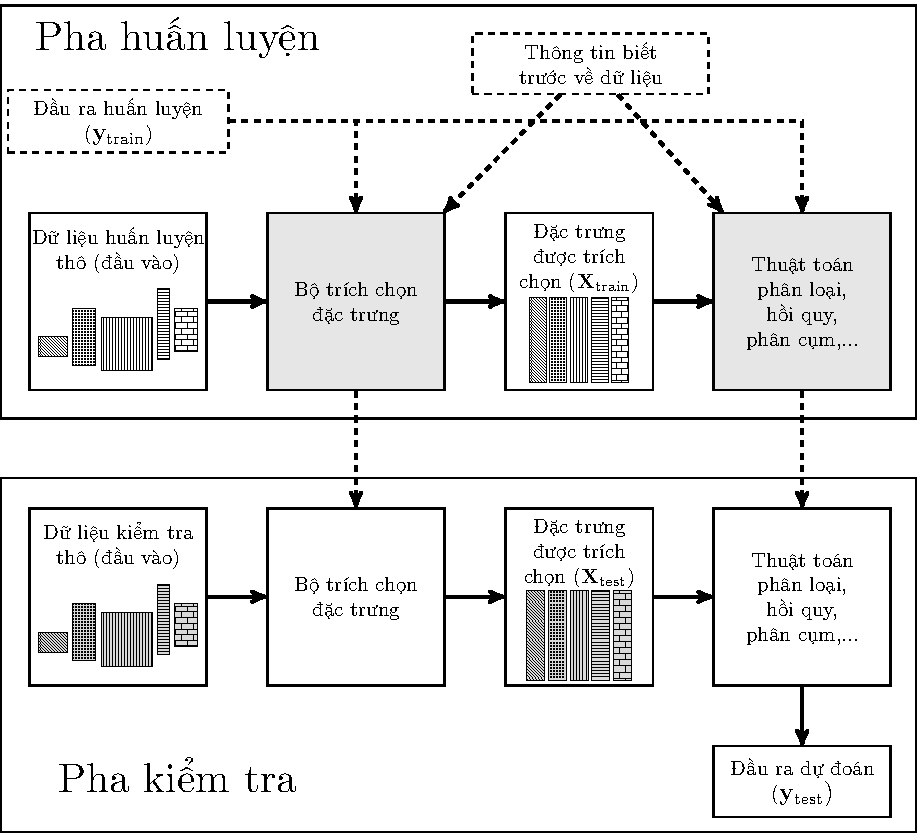
\includegraphics[width = \textwidth]{Chapters/01_Overview/11_featureengineering/latex/ML_models2.pdf}
\caption[]{Mô hình chung trong các bài toán machine learning}
\label{fig:11_1}
\end{figure}
% ******************************************************************************


% Với các bài toán supervised learning, ta có các cặp dữ liệu (\textit{input,
% output}), với các bài toán unsupervised learing, ta chỉ có \textit{input}. Khi
% thực hiện một thuật toán machine learning, toàn bộ dữ liệu có được thường được
% chia làm hai tập hợp không giao nhau: tập huấn luyện và tập kiểm thử. Với các
% thuật toán supervised learning, khi phân chia, ta cần chú ý phân chia đúng các
% cặp (\textit{input}, \textit{output}) của dữ liệu.

Phần lớn các mô hình machine learning có thể được minh hoạ trong
Hình~\ref{fig:11_1}. Có hai pha lớn trong mỗi bài toán machine learning là
\textit{pha huấn luyện} (training phase) và \textit{pha kiểm tra} (test phase). Pha huấn luyện xây dựng mô
hình dựa trên dữ liệu huấn luyện. Dữ liệu kiểm tra được sử dụng để đánh giá
hiệu quả mô hình\footnote{Trước khi đánh giá một mô hình trên tập kiểm tra, ta
cần đảm bảo rằng mô hình đó đã làm việc tốt trên tập huấn luyện.}.

\subsection{Pha huấn luyện}
Có hai khối có nền màu xám cần được thiết kế:

Khối trích chọn đặc trưng có nhiệm vụ tạo ra một
vector đặc trưng cho mỗi điểm dữ liệu đầu vào. Vector đặc trưng này thường có
kích thước như nhau, bất kể dữ liệu đầu vào có kích thước như thế nào.

Đầu vào của khối trích chọn đặc trưng có thể là các yếu tố sau:

\begin{itemize}
\item \textit{Dữ liệu huấn luyện đầu vào ở dạng thô} bao gồm tất cả các thông tin ban đầu. Ví dụ, dữ liệu thô của một ảnh là
giá trị của từng điểm ảnh, của một văn bản là từng từ, từng câu; của một
file âm thanh là một đoạn tín hiệu; của thời tiết là thông tin về hướng gió,
nhiệt độ, độ ẩm không khí,... Dữ liệu thô này thường không ở dạng vector,
không có số chiều như nhau hoặc một vài thông tin bị khuyết. Thậm chí chúng
có thể có số chiều như nhau nhưng rất lớn. Chẳng hạn, một bức ảnh màu kích
thước $1000\times 1000$ có số điểm ảnh là $3 \times 10^6$\footnote{Ảnh màu
thường có ba kênh: red, green, blue -- RGB}. Đây là một con số quá lớn, không có lợi cho lưu
trữ và tính toán.

\item \textit{Dữ liệu huấn luyện đầu ra}: dữ liệu này có thể được sử dụng
hoặc không. Trong các thuật toán học không giám sát, ta không biết đầu ra
nên hiển nhiên không có giá trị này. Trong các thuật toán học có giám sát,
đôi khi dữ liệu này cũng không được sử dụng. Ví dụ, việc giảm chiều dữ liệu
có thể không cần sử dụng dữ liệu đầu ra. Nếu dữ liệu đầu vào đã là các
vector cột cùng chiều, ta chỉ cần nhân vào bên phải của chúng một ma trận
chiếu ngẫu nhiên. Ma trận này có số hàng ít hơn số cột để đảm bảo số chiều
thu được nhỏ hơn số chiều ban đầu. Việc làm này mặc dù làm mất đi thông tin,
trong nhiều trường hợp vẫn mang lại hiệu quả vì đã giảm được lượng tính toán
ở phần sau. Đôi khi {ma trận chiếu} không phải là ngẫu nhiên mà có thể được
\textit{học} dựa trên toàn bộ dữ liệu thô ban đầu (xem Chương~\ref{cha:pca}).

Trong nhiều trường hợp khác, dữ liệu đầu ra của tập huấn luyện cũng được sử
dụng để tạo bộ trích chọn đặc trưng. Việc giữ lại
nhiều thông tin không quan trọng bằng việc giữ lại các thông tin có ích. Ví dụ, dữ liệu thô là các hình vuông và hình tam giác màu đỏ và xanh.
Trong bài toán phân loại đa giác, nếu các nhãn là \textit{tam giác} và
\textit{vuông}, ta không quan tâm tới màu sắc mà chỉ quan tâm tới số cạnh
của đa giác. Ngược lại, trong bài toán phân loại màu với các nhãn là
\textit{xanh} và \textit{đỏ}, ta không quan tâm tới số cạnh mà chỉ quan tâm
đến màu sắc.

\item \textit{Các thông tin biết trước về dữ liệu}: Ngoài dữ liệu huấn luyện, các thông tin biết trước ngoài lề cũng có tác dụng trong việc xây dựng bộ trích chọn đặc trưng. Chẳng hạn, có thể dùng các bộ lọc để giảm nhiễu nếu dữ liệu là âm thanh, hoặc dùng các bộ dò cạnh để tìm ra cạnh của các vật thể trong dữ liệu ảnh. Nếu dữ liệu là ảnh các tế bào và ta cần đưa ảnh về kích thước nhỏ hơn, ta cần lưu ý về độ phân giải của tế bảo của ảnh trong kích thước mới. Ta cần xây dựng một bộ trích chọn đặc trưng phù hợp với từng loại dữ liệu.
\end{itemize}

\index{dac@đặc trưng đã trích xuất -- extracted feature}
\index{extracted feature -- đặc trưng đã trích xuất}
Sau khi xây dựng bộ trích chọn đặc trưng, dữ liệu thô ban đầu được đưa qua và
tạo ra các vector đặc trưng tương ứng gọi là \textit{đặc trưng đã trích
xuất} ({extracted feature}). Những đặc trưng này được dùng để huấn luyện
các thuật toán machine learning chính như phân loại, phân cụm, hồi quy,... trong
khối màu xám thứ hai.

% \index{state-of-the-art}
\index{end-to-end}
\newnote{}{
Trong một số thuật toán cao cấp hơn, việc xây dựng bộ trích chọn đặc trưng và
các thuật toán chính có thể được thực hiện đồng thời thay vì riêng lẻ như trên.
Đầu vào của toàn bộ mô hình là dữ liệu thô hoặc dữ liệu thô đã qua một bước xử
lý nhỏ. Các mô hình đó có tên gọi chung là `mô hình đầu cuối' (end-to-end
model). Với sự phát triển của deep learning trong những năm gần đây, người ta
cho rằng các mô hình đầu cuối mang lại kết quả tốt hơn nhờ vào việc hai khối
được huấn luyện cùng nhau, bổ trợ lẫn nhau cùng hướng tới mục đích chung cuối
cùng. Thực tế cho thấy, các mô hình machine learning hiệu quả nhất thường là các
mô hình đầu cuối. }

%     Khi xây dựng bộ \textit{feature extractor} và \textit{main algorithms},
%     chúng ta không được sử dụng bất kỳ thông tin nào trong tập \textit{test data}. Ta phải giả sử rằng những thông tin trong \textit{test data} chưa được nhìn thấy bao giờ. Nếu sử dụng thêm thông tin về \textit{test data} thì rõ ràng ta đã \textit{ăn gian}
% \end{mynote}

% \textbf{Một điểm rất quan trọng: khi xây dựng bộ \textit{feature extractor} và \textit{main algorithms}, chúng ta không được sử dụng bất kỳ thông tin nào trong tập \textit{test data}. Ta phải giả sử rằng những thông tin trong \textit{test data} chưa được nhìn thấy bao giờ. Nếu sử dụng thêm thông tin về \textit{test data} thì rõ ràng ta đã \textit{ăn gian}! Tôi từng đánh giá các bài báo khoa học quốc tế, rất nhiều tác giả xây dựng mô hình dùng cả dữ liệu \textit{test data}, sau đó lại dùng chính mô hình đó để kiểm tra trên \textit{test data} đó. Việc \textit{ăn gian} này là lỗi rất nặng và hiển nhiên những bài báo đó bị từ chối (reject).}


\subsection{Pha kiểm tra}

Ở pha kiểm tra, vector đặc trưng của một điểm dữ liệu thô mới được tạo bởi bộ trích chọn đặc trưng thu được từ pha huấn luyện. Vector đặc trưng này được đưa
vào thuật toán chính đã tìm được để đưa ra quyết tra. Có một lưu ý quan trọng là khi xây dựng bộ trích chọn đặc trưng và các thuật toán chính, ta không được sử dụng dữ liệu kiểm tra. Các công việc đó được thực hiện chỉ dựa trên dữ liệu huấn luyện.

% Bước này đơn giản hơn nhiều. Với \textit{raw input} mới, ta sử dụng feature
% extractor đã tạo được ở trên (tất nhiên không được sử dụng \textit{output} của nó vì \textit{output} là cái ta đang đi tìm) để tạo ra feature vector tương ứng. Feature vector được đưa vào \textit{main algorithm} đã được học ở training phase để dự đoán \textit{output}.


\section{Một số kỹ thuật trích chọn đặc trưng}

\subsection{Trực tiếp lấy dữ liệu thô}
% Với bài toán phân loại chữ số viết tay trong bộ cơ sở dữ liệu \href{http://machinelearningcoban.com/2017/01/04/kmeans2/#bo-co-so-du-lieu-mnist}{MNIST}, mỗi bức ảnh có số chiều là 28 điểm ảnh x 28 điểm ảnh (tất nhiên việc \textit{crop} và chỉnh sửa mỗi bức ảnh đã được thực hiện từ trước rồi, đó đã là một phần của feature engineering rồi). Một cách đơn giản thường được dùng là \textit{kéo dài} ma trận 28x28 này để được 1 vector có số chiều 784. Trong cách này, các cột (hoặc hàng) của ma trận ảnh được đặt chồng lên (hoặc cạnh nhau) để được 1 vector dài. Vector dài này được trực tiếp sử dụng làm feature đưa vào các bộ classifier/clustering/regression/... Lúc này, giá trị của mỗi điểm ảnh ảnh được coi là một feature.

\index{vectorization -- vector hoá}
\index{vector hoá -- vectorization}
Xét bài toán với dữ liệu là các bức ảnh xám có kích thước cố tra $m\times n$
điểm ảnh. Cách đơn giản nhất để tạo ra vector đặc trưng cho bức ảnh này là xếp
chồng các cột của ma trận điểm ảnh để được một vector $m\times n$ phần tử.
Vector này có thể được coi là vector đặc trưng với mỗi đặc trưng là giá trị của
một điểm ảnh. Việc làm đơn giản này đã làm mất {thông tin về vị trí tương đối}
giữa các điểm ảnh vì các điểm ảnh gần nhau theo phương ngang trong bức ảnh ban
đầu không còn gần nhau trong vector đặc trưng. Tuy nhiên, trong
nhiều trường hợp, kỹ thuật này vẫn mang lại kết quả khả quan.

\subsection{Lựa chọn đặc trưng}
\index{lựa chọn đặc trưng -- feature selection}
\index{feature selection -- lựa chọn đặc trưng}
Đôi khi, việc trích chọn đặc trưng đơn giản là chọn ra các thành phần phù hợp trong dữ liệu ban đầu. Việc làm này thường xuyên được áp dụng khi một lượng dữ liệu thu được không có đầy đủ các thành phần hoặc dữ liệu có quá nhiều chiều mà phần lớn không mang nhiều thông tin hữu ích.

\subsection{Giảm chiều dữ liệu}
\index{giảm chiều dữ liệu -- dimensionality reduction}
\index{dimensionality reduction -- giảm chiều dữ liệu}
% \index{chiếu ngẫu nhiên -- random projection}
\index{ma trận chiếu -- projection matrix}
\index{projection matrix -- ma trận chiếu}
\index{phân tích thành phần chính -- principal component analysis}
\index{principal component analysis -- phân tích thành phần chính}
Giả sử dữ liệu ban đầu là một vector $\bx \in \R^D$, $\bA$ là một ma trận trong
$R^{d\times D}$ và $\bz = \bA\bx\in\R^d$. Nếu $d < D$, ta thu được một vector
với số chiều nhỏ hơn. Đây là một kỹ thuật phổ biến trong giảm chiều dữ liệu. Ma
trận $\bA$ được gọi là \textit{ma trận chiếu} (projection matrix), có thể là một ma trận ngẫu nhiên.
Tuy nhiên, việc chọn một ma trận chiếu ngẫu nhiên đôi khi mang lại kết quả tệ
không mong muốn vì thông tin có thể bị thất thoát quá nhiều. Một phương pháp phổ
biến để tối thiểu lượng thông tin mất đi có tên là \textit{phân tích thành phần
chính} ({principal component analysis}) sẽ được trình bày trong
Chương~\ref{cha:pca}.

\textit{Lưu ý:} {Kỹ thuật xây dựng đặc trưng không nhất thiết luôn làm giảm số
chiều dữ liệu, đôi khi vector đặc trưng có thể có có kích thước lớn hơn dữ liệu
thô ban đầu nếu việc này mang lại hiệu quả tốt hơn.}

% feature vector còn có số chiều lớn hơn raw data.
% Random projection
% cũng có thể làm được việc này nếu ma trận chiếu là một ma trận \textit{cao} (số
% cột ít hơn số hàng).


\subsection{Túi từ}
\index{túi từ -- bag of words}
\index{bag of words -- túi từ}

Chúng ta hẳn đã tự đặt ra các câu hỏi: với một văn bản, vector đặc trưng sẽ có
dạng như thế nào? Làm sao đưa các từ, các câu, đoạn văn ở dạng ký tự
trong các văn bản về một vector mà mỗi phần tử là một số?

Có một kỹ thuật rất phổ biến trong xử lý văn bản có tên là \textit{túi từ}
({bag of words, BoW}).

Bắt đầu bằng ví dụ phân loại tin nhắn rác. Nhận thấy rằng nếu một tin có chứa
các từ {``khuyến mại'', ``giảm giá'', ``trúng thưởng'', ``miễn phí'', ``quà tặng'', ``tri
ân'',...}, nhiều khả năng đó là một tin nhắn rác. Từ đó, phương pháp đầu tiên có
thể nghĩ tới là {đếm} số lần các từ này xuất hiện, nếu số lượng này nhiều hơn
một ngưỡng nào đó thì ta quyết định đó là tin rác\footnote{Bài toán thực tế phức
tạp hơn khi các tin nhắn có thể được viết dưới dạng không dấu, bị cố tình viết
sai chính tả, hoặc dùng các ký tự đặc biệt}. Với các loại văn bản khác nhau,
lượng từ liên quan tới từng chủ đề cũng khác nhau. Từ đó có thể dựa vào số lượng
các từ trong từng loại để tạo các vector đặc trưng cho từng văn bản.

% Tôi xin lấy ví dụ cụ thể hơn về cách tạo ra vector đặc trưng cho mỗi văn bản dựa trên BoW và xin được lấy tiếng Anh làm ví dụ (nguồn \href{https://en.wikipedia.org/wiki/Bag-of-words_model}{Bag of Words wiki}. Tiếng Việt khó hơn vì một từ có thể có nhều âm tiết, tiếng Anh thì thường cứ gặp dấu cách là kết thúc một từ).
% \newpage
\index{túi từ -- bag of words!từ điển}
\index{bag of words -- túi từ!từ điển}
Xin lấy một ví dụ về hai văn bản đơn giản sau đây\footnote{\textit{Bag of
words -- Wikipedia} (\url{https://goo.gl/rBtZqx})}:

\begin{lstlisting}[language=Python]
(1) "John likes to watch movies. Mary likes movies too."
\end{lstlisting}
và
\begin{lstlisting}[language=Python]
(2) "John also likes to watch football games."
\end{lstlisting}
Dựa trên hai văn bản này, ta có danh sách các từ được sử dụng, được gọi là
\textit{từ điển} ({dictionary} hoặc {codebook}) với mười
\textit{từ} như sau:

\begin{lstlisting}[language=Python]
["John", "likes", "to", "watch", "movies", "also", "football", "games", "Mary", "too"]
\end{lstlisting}
Với mỗi văn bản, ta sẽ tạo ra một vector đặc trưng có số chiều bằng 10, mỗi phần
tử đại diện cho số từ tương ứng xuất hiện trong văn bản đó. Với hai văn bản
trên, ta sẽ có hai vector đặc trưng:
\begin{lstlisting}[language=Python]
(1) [1, 2, 1, 1, 2, 0, 0, 0, 1, 1]
(2) [1, 1, 1, 1, 0, 1, 1, 1, 0, 0]
\end{lstlisting}
Văn bản (1) có một từ \pythoninline{"John"}, hai từ \pythoninline{"likes"}, không từ
\pythoninline{"also"}, không từ \pythoninline{"football"},... nên ta thu được
vector tương ứng như trên.

\index{vector thưa -- sparse vector}
\index{sparse vector -- vector thưa}
Có một vài điều cần lưu ý trong BoW:
\begin{itemize}
\item Với những ứng dụng thực tế, {từ điển} có số lượng từ lớn hơn rất
nhiều, có thể đến cả triệu, như vậy vector đặc trưng thu được sẽ rất dài.
Một văn bản chỉ có một câu, và một tiểu thuyết nghìn trang đều được biểu
diễn bằng các vector có kích thước như nhau.

\item Có rất nhiều từ trong từ điển không xuất hiện trong một văn bản. Như
vậy các vector đặc trưng thu được thường có nhiều phần tử bằng không.
Các vector đó được gọi là \textit{vector thưa} (sparse vector). Để việc lưu trữ được hiệu quả hơn, ta không lưu mọi thành phần của một
vector thưa mà chỉ lưu {vị trí} của các phần tử khác không và {giá
trị} tương ứng. Chú ý rằng nếu có hơn một nửa số phần tử khác không, việc
làm này lại phản tác dụng. Tuy nhiên, trường hợp này ít xảy ra vì hiếm có
văn bản chứa tới một nửa số từ trong từ điển.

\item Các từ hiếm gặp được xử lý như thế nào? Một kỹ thuật thường dùng là
thêm phần tử \pythoninline{<Unknown>} vào trong từ điển. Mọi từ không có
trong từ điển đều được coi là
\pythoninline{<Unknown>}.

\item Tuy nhiên, những từ hiếm đôi khi lại mang những thông tin quan
trọng nhất mà chỉ loại văn bản đó có. Đây là một nhược điểm của BoW. Có một
phương pháp cải tiến giúp khắc phục nhược điểm này tên là \textit{term
frequency-inverse document frequency} (TF-IDF)~\cite{salton1975vector} dùng
để xác định tầm quan trọng của một từ trong một văn bản dựa trên toàn bộ văn
bản trong cơ sở dữ liệu\footnote{\textit{5 Algorithms Every Web Developer
Can Use and Understand, section 5} (\url{https://goo.gl/LJW3H1}).}.

\item Nhược điểm lớn nhất của BoW là nó không mang thông tin về thứ tự của
các từ, cũng như sự liên kết giữa các câu, các đoạn văn trong văn bản. Thứ
tự của các từ trong văn bản thường mang thông tin quan trọng. Ví dụ, ba câu
sau đây: ``Em yêu anh không?'', ``Em không yêu anh'', và ``Không, (nhưng)
anh yêu em'' khi được trích chọn đặc trưng bằng BoW sẽ cho ra ba vector
giống hệt nhau, mặc dù ý nghĩa khác hẳn nhau.
\end{itemize}

% \textbf{Bonus:} hình dưới đay là tần suất sử dụng các từ (coi mỗi âm tiết là một từ) trong Truyện Kiều (\href{https://bitbucket.org/tiepvupsu/vietnamese/src/c6f3af6050f8ca911ed0fa209220ce3c99010075/TruyenKieu2.txt?at=master&fileviewer=file-view-default}{theo bản này}) nếu ta chỉ sử dụng 30 từ có tần suất cao nhất. :
% <div class="imgcap">
% <img src ="\assets\FeatureEngineering\truyenkieu.png" align = "center" width = "400">
% <div class = "thecap">Hình 2: Bag of Words cho Truyện Kiều với 30 từ có tần suất cao nhất.</div>
% </div>


\subsection{BoW cho dữ liệu ảnh}
BoW cũng được áp dụng cho các bức ảnh với cách định nghĩa \textit{từ} và
\textit{từ điển} khác. Xét các ví dụ sau:

\textit{Ví dụ 1}: Giả sử có một tập dữ liệu ảnh có hai nhãn là rừng và sa mạc, và một bức ảnh chỉ rơi vào một trong hai loại này. Việc phân
loại một bức ảnh là rừng hay sa mạc một cách tự nhiên nhất là dựa vào màu sắc.
Màu xanh lục nhiều tương ứng với rừng, màu đỏ và vàng nhiều tương ứng với sa mạc. Ta có một mô hình đơn giản để trích chọn đặc trưng như sau:
\begin{itemize}
\item Với một bức ảnh, chuẩn bị một vector $\mathbf{x}$ có số chiều bằng 3,
đại diện cho ba màu xanh lục ($x_1$), đỏ ($x_2$), và vàng ($x_3$).

\item Với mỗi điểm ảnh trong bức ảnh đó, xem nó gần với màu xanh, đỏ hay
vàng nhất dựa trên giá trị của điểm ảnh đó. Nếu nó gần điểm xanh nhất, tăng
$x_1$ lên một; gần đỏ nhất, tăng $x_2$ lên một; gần vàng nhất, tăng $x_3$
lên một.

\item Sau khi xem xét tất cả các điểm ảnh, dù cho bức ảnh có kích thước thế
nào, ta vẫn thu được một vector có kích thước bằng ba, mỗi phần tử thể hiện
việc có bao nhiêu điểm ảnh trong bức ảnh có màu tương ứng. Vector cuối này còn
được gọi là \textit{histogram vector} của bức ảnh và có thể coi là một vector đặc trưng tốt trong bài toán phân loại
ảnh rừng hay say mạc.
\end{itemize}

\textit{Ví dụ 2}: Trên thực tế, các bài toán xử lý ảnh không đơn giản như trong
ví dụ trên đây. Mắt người thực ra nhạy với các đường nét, hình dáng hơn là màu
sắc. Chúng ta có thể nhận biết được một bức ảnh có cây hay không ngay cả khi bức
ảnh đó không có màu. Vì vậy, xem xét giá trị từng điểm ảnh không mang lại kết
quả khả quan vì lượng thông tin về đường nét đã bị mất.

\index{patch}
% ******************************************************************************
\begin{figure}[t]
\centering
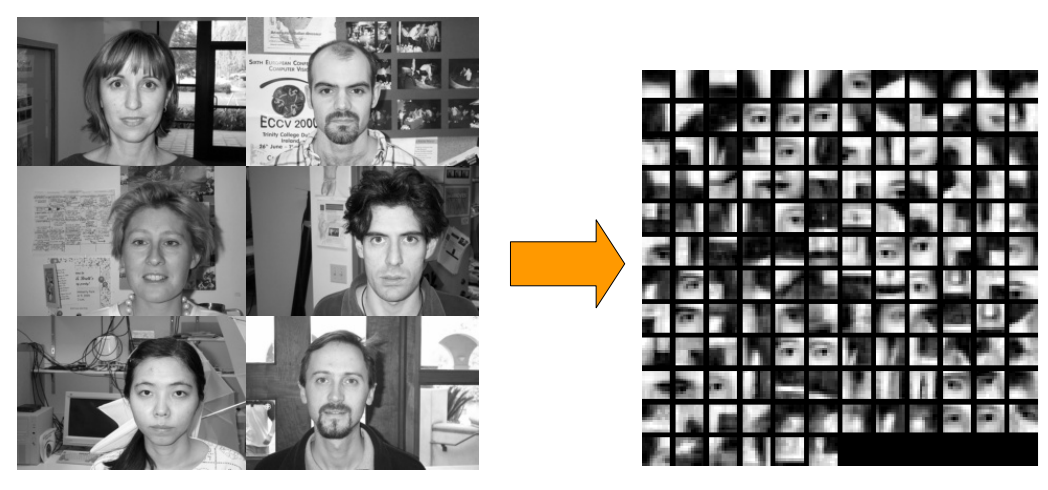
\includegraphics[width = \textwidth]{Chapters/01_Overview/11_featureengineering/bow_face.png}
\caption[]{Bag of words cho ảnh chứa mặt người (Nguồn: \textit{Bag of
visual words model: recognizing object categories}
(\url{https://goo.gl/EN2oSM}).}
\label{fig:11_2}
\end{figure}
% ******************************************************************************

Có một giải pháp là thay vì xem xét một điểm ảnh, ta xem xét một vùng hình chữ
nhật nhỏ trong ảnh, vùng này còn được gọi là \textit{patch}. Các patch này nên
đủ lớn để có thể chứa được các bộ phận đặc tả vật thể trong ảnh. Ví dụ với mặt
người, các patch cần chứa được các phần của khuôn mặt như mắt, mũi, miệng (xem
Hình~\ref{fig:11_2}). Tương tự, với ảnh là ô tô, các patch thu được có thể là
bánh xe, khung xe, cửa xe,...(xem Hình~\ref{fig:11_3}, hàng trên bên phải).
\begin{figure}[t]
\centering
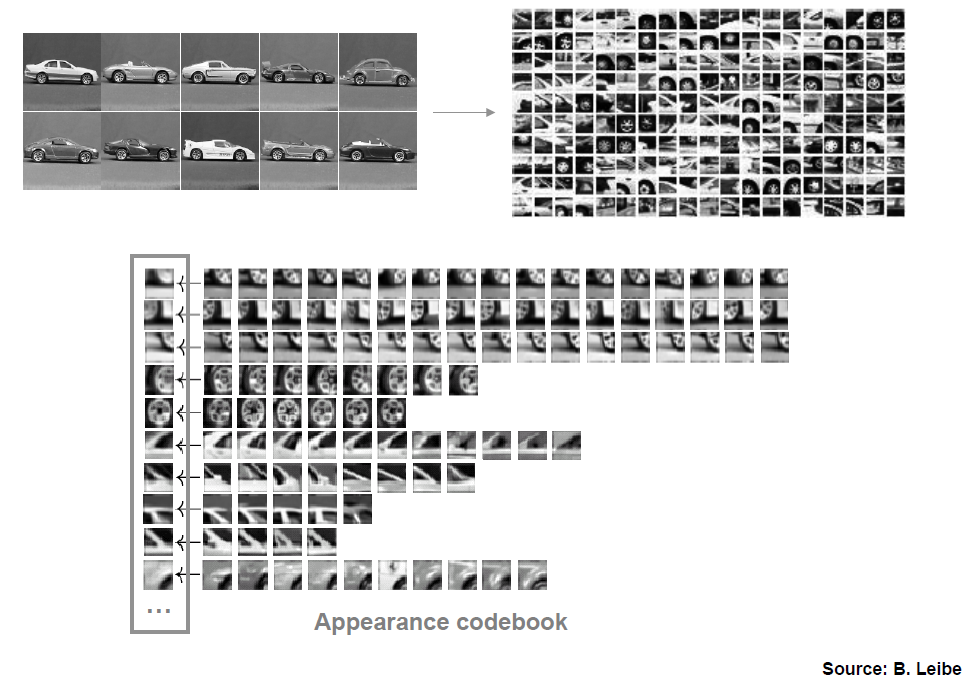
\includegraphics[width = \textwidth]{Chapters/01_Overview/11_featureengineering/bow_car.png}
\caption[]{Bag of Words cho ảnh xe hơi (Nguồn: B. Leibe).}
\label{fig:11_3}
\end{figure}
% <div class="imgcap">
% <img src ="\assets\FeatureEngineering\bow_car.png" align = "center" width = "800">
% <div class = "thecap">Hình 4: Bag of Words cho ảnh ô tô. (Nguồn: tôi cố gắng tìm nguồn cho hình này nhưng tất cả các tài liệu tôi tìm được đều ghi "Source: B. Leibe", tôi cũng xin được trích nguồn tương tự)</div>
% </div>

Trong xử lý văn bản, hai từ được coi là như nhau nếu nó được biểu diễn bởi các
ký tự giống nhau. Câu hỏi đặt ra là, trong xử lý ảnh, hai patch được coi là như
nhau khi nào? Khi mọi điểm ảnh trong hai patch có giá trị bằng nhau sao?

Câu trả lời là không. Xác suất để hai patch giống hệt nhau từng điểm ảnh là rất
thấp vì có thể một phần của vật thể trong một patch bị lệch đi, bị
méo, hoặc có độ sáng thay đổi. Trong những trường hợp này, mặc dù mắt người vẫn
thấy hai patch đó {rất giống nhau}, máy tính có thể nghĩ đó là hai patch
khác nhau. Vậy, hai patch được coi là như nhau khi nào? Từ và {từ điển} ở
đây được định nghĩa như thế nào?

% Hai patch được coi là gần giống nhau nếu
% khoảng cách Euclid giữa hai vector tạo bởi hai patch đó là nhỏ. Từ điển sẽ được xây dựng có số
% từ do ta tự chọn. Số từ trong từ điển càng cao thì độ sai lệch càng ít, nhưng yêu cầu cao hơn về tính toán.

Ta có thể áp dụng một phương pháp phân cụm đơn giản là $K$-means
(xem Chương~\ref{cha:kmeans}) để tạo ra từ điển và coi hai patch là gần nhau nếu
khoảng cách Euclid giữa hai vector tạo bởi hai patch là nhỏ. Với rất nhiều patch
thu được, giả sử cần xây dựng một từ điển với chỉ khoảng 1000 \textit{từ}, ta có
thể dùng phân cụm $K$-means để phân toàn bộ các patch thành 1000 cụm (mỗi
cụm được coi là một \textit{bag}) khác nhau. Mỗi cụm gồm các patch gần giống
nhau, được mô tả bởi trung bình cộng của tất cả các patch trong cụm đó (xem
Hình~\ref{fig:11_3} hàng dưới). Với một ảnh bất kỳ, ta trích ra các patch từ ảnh
đó, tìm xem mỗi patch gần với cụm nào nhất trong 1000 cụm tìm được ở trên và
quyết định patch này thuộc cụm đó. Cuối cùng, ta sẽ thu được một vector đặc
trưng có kích thước bằng 1000 mà mỗi phần tử là số lượng các patch trong ảnh rơi
vào cụm tương ứng.

% \subsection{Transfer learning}
%!TEX root = ../../book_ML.tex
\section{Học chuyển tiếp cho bài toán phân loại ảnh}
% (\textit{Giả sử rằng bạn đọc đã có kiến thức nhất định về deep neural network.})
Mục này được viết trên cơ sở bạn đọc đã có kiến thức nhất định và deep learning.
% Trước khi deep learning ra đời, bài toán phân loại ảnh (các loại dữ liệu khác cũng tương tự) thường được chia thành hai bước: Feature Engineering và Train a Classifier. Hai bước này thường được tách rời nhau. 

Ngoài BoW, các phương pháp phổ biến được sử dụng để xây dựng vector đặc trưng cho ảnh là \textit{scale invariant feature transform -- SIFT}~\cite{lowe1999object}, \textit{speeded-up robust features -- SURF}~\cite{bay2006surf}, \textit{histogram of oriented gradients -- HOG}~\cite{dalal2005histograms}, \textit{local binary pattern -- LBP}~\cite{lowe1999object},... Các bộ phân loại thường được sử dụng là SVM đa lớp (Chương~\ref{cha:multisvm}), {hồi quy softmax} (Chương~\ref{cha:softmax}), mã hóa thưa và học từ điển~\cite{wright2009robust,vu2016histopathological,vu2016fast}, rừng ngẫu nhiên~\cite{liaw2002classification},... 



% Với Feature Engineering, các phương pháp thường được sử dụng cho ảnh là \href{http://docs.opencv.org/3.1.0/da/df5/tutorial_py_sift_intro.html}{SIFT} (Scale Invariant Feature Transform), \href{http://docs.opencv.org/3.0-beta/doc/py_tutorials/py_feature2d/py_surf_intro/py_surf_intro.html}{SURF} (Speeded-Up Robust Features), \href{http://www.learnopencv.com/histogram-of-oriented-gradients/}{HOG} (Histogram of Oriented Gradients), LBP (Local Binary Pattern), etc. Các Classifier thường được sử dụng là \href{http://machinelearningcoban.com/2017/04/28/multiclasssmv/}{multi-class SVM}, \href{http://machinelearningcoban.com/2017/02/17/softmax/}{Softmax Regression}, Discriminative Dictionary Learning, Random Forest, etc. 
\index{dac@đặc trưng thủ công -- hand-crafted feature} 
Các đặc trưng được tạo bởi các phương pháp nêu trên thường được gọi là các
\textit{đặc trưng thủ công} ({hand-crafted feature}) vì chúng chủ yếu dựa
trên các quan sát về đặc tính riêng của ảnh và được xây dựng chung cho mọi loại
dữ liệu ảnh. Các phương pháp này cho kết quả khá ấn tượng trong một số trường
hợp. Tuy nhiên, chúng vẫn còn nhiều hạn chế vì quá trình tìm ra các đặc trưng và
các bộ phân loại là riêng biệt. Hơn nữa, các bộ trích chọn này chỉ tìm ra các
\textit{đặc trưng mức thấp} ({low-level features}) của ảnh.

Những năm gần đây, deep learning phát triển cực nhanh dựa trên lượng dữ liệu
huấn luyện khổng lồ và khả năng tính toán ngày càng được cải tiến của các máy
tính. Kết quả cho bài toán phân loại ảnh ngày càng được nâng cao. Bộ cơ sở dữ
liệu thường được dùng nhất là ImageNet (\url{https://www.image-net.org}) với 1.2
triệu ảnh cho 1000 nhãn khác nhau. Rất nhiều mô hình deep learning đã giành
chiến thắng trong các cuộc thi \textit{ImageNet large scale visual recognition
challenge -- ILSVRC} (\url{https://goo.gl/1A8drd}):
AlexNet~\cite{krizhevsky2012imagenet}, ZFNet~\cite{zeiler2014visualizing},
GoogLeNet~\cite{szegedy2015going}, ResNet~\cite{he2016deep},
VGG~\cite{simonyan2014very}. Nhìn chung, các mô hình này là các \textit{mạng neuron đa tầng} (multi-layer neural network). Các tầng phía trước thường là các \textit{tầng tích chập} (convolutional layer). Tầng cuối cùng là một \textit{tầng nối kín} (fully connected layer) và thường là một bộ hồi quy
softmax (xem Hình~\ref{fig:transferlearning}). Vì vậy đầu ra của tầng gần cuối
cùng có thể được coi là vector đặc trưng và hồi quy softmax chính là bộ phân
loại được sử dụng\footnote{hồi quy softmax là một thuật toán phân loại, tên gọi \textit{hồi quy} của nó mang tính lịch sử.}.
 
Việc bộ trích chọn đặc trưng và bộ phân loại được huấn luyện cùng nhau thông qua
tối ưu hệ số trong mạng neuron sâu khiến các mô hình này đạt kết quả tốt. Tuy
nhiên, những mô hình này đều bao gồm rất nhiều tầng các trọng số. Việc huấn
luyện dựa trên hơn một triệu bức ảnh tốn rất nhiều thời gian (2-3 tuần).
 
\index{học chuyển tiếp -- transfer learning}
Với các bài toán phân loại các dữ liệu ảnh khác với tập huấn luyện nhỏ, ta có
thể không cần xây dựng lại mạng neuron và huấn luyện nó từ đầu. Thay vào đó, ta có
thể sử dụng các mô hình đã được huấn luyện nêu trên và thay đổi kiến trúc của mạng cho phù hợp. Phương pháp sử dụng các mô hình có sẵn như vậy còn
được gọi là \textit{học chuyển tiếp} ({transfer learning}).
 
Toàn bộ các tầng trừ tầng đầu ra có thể được coi là một bộ trích chọn đặc trưng.
Điều này được rút ra dựa trên nhận xét rằng các bức ảnh thường có những đặc tính
giống nhau. Sau đó, ta huấn luyện một bộ phân loại khác dựa trên
vector đặc trưng đã đã được trích chọn. Cách làm này có thể tăng độ chính xác
phân loại lên đáng kể so với việc sử dụng các đặc trưng thủ công vì các mạng neuron sâu được cho là có khả năng trích chọn các \textit{đặc trưng mức cao} ({high-level features}) của ảnh. 

 
%% *****************************************************************************
\begin{figure}[t]
\centering
    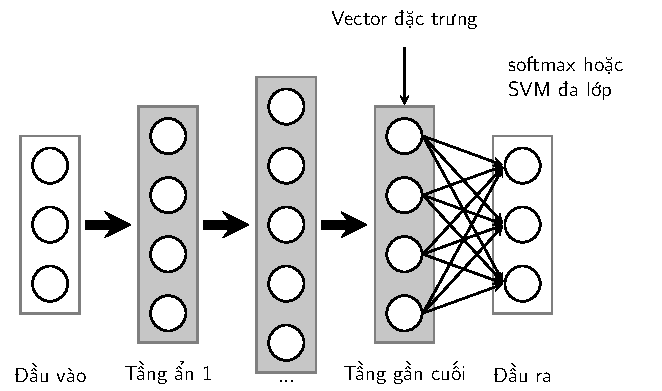
\includegraphics[width = \textwidth]{Chapters/01_Overview/q2_tl/latex/multi_layers.pdf}
    \caption[]{Kiến trúc deep learning cơ bản cho bài toán phân loại. Tầng cuối cùng là một tầng nối kín và thường là một hồi quy softmax.}
    \label{fig:transferlearning}
\end{figure}
%% ***************************************************************************** 
\index{tinh chỉnh -- fine-tuning}
Hướng tiếp cận thứ hai là sử dụng các mô hình đã được huấn luyện và cho huấn luyện thêm một vài tầng cuối dựa trên dữ liệu mới. Kỹ thuật này được
gọi là \textit{tinh chỉnh} ({fine-tuning}). {Việc này được thực hiện dựa trên quan
sát rằng những tầng đầu trong mạng neuron sâu trích xuất những đặc trưng chung mức thấp của đa số ảnh, các tầng cuối giúp trích chọn các đặc trưng mức cao phù hợp cho từng cơ sở dữ liệu (CSDL). Các đặc trưng mức cao có thể khác nhau tuỳ theo từng CSDL. Vì vậy, khi có dữ liệu mới, ta chỉ cần huấn luyện mạng neuron để trích chọn các đặc trưng mức cao phù hợp với dữ liệu mới này. 
 
Dựa trên kích thước và sự giống nhau giữa CSDL mới và CSDL gốc (dùng để huấn luyện mạng neuron ban đầu), có một vài quy tắc để huấn luyện mạng neuron mới\footnote{\textit{Transfer Learning, CS231n} (\url{https://goo.gl/VN1g7F})}: 

\begin{itemize}
\item \textit{CSDL mới nhỏ, tương tự CSDL gốc.} Vì CSDL mới nhỏ, việc
tiếp tục huấn luyện mô hình có thể dễ dẫn đến hiện tượng \textit{quá khớp} (overfitting, xem Chương~\ref{cha:overfitting}). Cũng vì hai CSDL tương tự nhau, ta dự đoán
rằng các đặc trưng mức cao của chúng tương tự nhau. Vì vậy, ta không cần
huấn luyện lại mạng neuron mà chỉ cần huấn luyện một bộ phân loại dựa trên các vector đặc trưng thu được. 
 
\item \textit{CSDL mới lớn, tương tự CSDL gốc.} Vì CSDL này lớn,
quá khớp ít xảy ra hơn, ta có thể huấn luyện mô hình thêm một
vài vòng lặp. Việc huấn luyện có thể được thực hiện trên toàn bộ hoặc chỉ một
vài tầng cuối.
 
\item \textit{CSDL mới nhỏ, rất khác CSDL gốc.} Vì CSDL này nhỏ, tốt
hơn hết là dùng các bộ phân loại đơn giản khác để tránh quá khớp. Nếu muốn sử
dụng mạng neuron cũ, ta cũng chỉ nên tinh chỉnh các tầng cuối của nó. Hoặc có thể coi đầu ra của một tầng ở giữa của mạng neuron là vector đặc
trưng rồi huấn luyện thêm một bộ phân loại.
 
\item \textit{CSDL mới lớn rất khác CSDL gốc.} Thực tế cho thấy, sử dụng
các mạng neuron sẵn có trên CSDL mới vẫn hữu ích. Trong trường hợp này, ta vẫn có
thể sử dụng các mạng neuron sẵn có như là điểm khởi tạo của mạng neuron mới, không nên
huấn luyện mạng neuron mới từ đầu.
\end{itemize}
 
Một điểm đáng chú ý là khi tiếp tục huấn luyện các mạng neuron này, ta chỉ
nên chọn tốc độ học nhỏ để các hệ số mới không đi quá xa so với các
hệ số đã được huấn luyện ở các mô hình trước.
 
 
 
 
 
% \section{Đọc thêm}
% [1] \href{http://docs.opencv.org/3.1.0/da/df5/tutorial_py_sift_intro.html}{Introduction to SIFT (Scale-Invariant Feature Transform) - OpenCV} 
 
% [2] \href{http://machinelearningcoban.comIntroduction to SURF (Speeded-Up Robust Features}{Introduction to SURF (Speeded-Up Robust Features) - OpenCV}) 
 
% [3] \href{http://www.learnopencv.com/histogram-of-oriented-gradients/}{Histogram of Oriented Gradients - OpenCV} 
 
% [4] \href{http://cs231n.github.io/transfer-learning/#tf}{Transfer Learning} 
 
% [5] \href{http://sebastianruder.com/transfer-learning/}{Transfer Learning - Machine Learning's Next Frontier} 
 
% [6] \href{https://www.analyticsvidhya.com/blog/2017/06/transfer-learning-the-art-of-fine-tuning-a-pre-trained-model/}{Transfer learning & The art of using Pre-trained Models in Deep Learning} 

\section{Chuẩn hoá vector đặc trưng}
% (Tham khảo \href{https://en.wikipedia.org/wiki/Feature_scaling}{Feature Scaling wiki}).

Các điểm dữ liệu đôi khi được đo đạc bằng những đơn vị khác nhau, chẳng hạn mét
và feet. Đôi khi, hai thành phần của dữ liệu ban đầu chênh lệch nhau lớn, chẳng
hạn một thành phần có khoảng giá trị từ 0 đến 1000, thành phần kia chỉ có khoảng
giá trị từ 0 đến 1. Lúc này, chúng ta cần chuẩn hóa dữ liệu trước khi thực hiện
các bước tiếp theo.

\textit{Chú ý}: việc chuẩn hóa này chỉ được thực hiện khi vector dữ liệu đã có cùng chiều.

Sau đây là một vài phương pháp chuẩn hóa thường dùng.

\index{chuyển khoảng giá trị -- rescaling}
\index{rescaling -- chuyển khoảng giá trị}
\subsection{Chuyển khoảng giá trị}
Phương pháp đơn giản nhất là đưa tất cả các đặc trưng về cùng một khoảng, ví dụ $[0, 1]$ hoặc $[-1, 1]$. Để muốn đưa đặc trưng thứ
$i$ của một vector đặc trưng $\bx$ về khoảng $[0, 1]$, ta sử dụng công thức
\begin{equation*}
x_i' = \frac{x_i - \min(x_i)}{\max(x_i) - \min(x_i)}
\end{equation*}
trong đó $x_i$ và $x_i'$ lần lượt là giá trị đặc trưng ban đầu và giá trị đặc
trưng sau khi được chuẩn hóa. $\min(x_i), \max(x_i)$ là giá trị nhỏ nhất và lớn
nhất của đặc trưng thứ $i$ xét trên toàn bộ dữ liệu huấn luyện.


\subsection{Chuẩn hoá theo phân phối chuẩn}
\index{chuẩn hoá theo phân phối chuẩn -- standardization}
\index{standardization -- chuẩn hoá theo phân phối chuẩn}
Một phương pháp khác thường được sử dụng là đưa mỗi đặc trưng về dạng một
phân phối chuẩn có kỳ vọng là 0 và phương sai là 1. Công thức chuẩn hóa
là
\begin{equation*}
x_i' = \frac{x_i - \bar{x}_i}{\sigma_i}
\end{equation*}
với $\bar{x}_i, \sigma_i$ lần lượt là kỳ vọng và độ lệch chuẩn của đặc trưng đó
xét trên toàn bộ dữ liệu huấn luyện.

\subsection{Chuẩn hoá về cùng norm}
Một lựa chọn khác cũng được sử dụng rộng rãi là biến vector dữ liệu thành vector
có độ dài Euclid bằng một. Việc này có thể được thực hiện bằng cách chia mỗi
vector đặc trưng cho $\ell_2$ norm của nó:
\begin{equation*}
\mathbf{x}' = \frac{\mathbf{x}}{\|\mathbf{x}\|_2}
\end{equation*}


% \section{Đọc thêm}
% \begin{enumerate}
%     \item  G. Csurka \etal, \textit{Visual categorization with bags
%     of keypoints}. Workshop on statistical learning in computer vision, ECCV.
%     Vol. 1. No. 1-22. 2004~\cite{csurka2004visual}.

%     \item S. Lazebnik \etal, \textit{Beyond bags
%         of features: Spatial pyramid matching for recognizing natural scene
%         categories.}, CVPR 2006~\cite{lazebnik2006beyond}

%     \item \textit{Preprocessing data, scikit learn}
%     (\url{https://goo.gl/gkCuUp}).

% \end{enumerate}


% \cite{bishop2006pattern}
%!TEX root = ../../book_ML.tex
\chapter{Hồi quy tuyến tính}
\label{cha:linear_regression}
\index{hồi quy tuyến tính -- linear regression}
\index{linear regression -- hồi quy tuyến tính}
% Trong chương này, chúng ta cùng làm quen với một trong những thuật toán machine
% learning  cơ bản nhất -- linear regression (hồi quy tuyến tính). Qua chương này,
% bạn đọc sẽ có cái nhìn ban đầu về việc xây dựng một hệ thống machine learning.
% Linear regression là một thuật toán supervised, ở đó quan hệ giữa đầu vào và đầu
% ra được mô tả bởi một hàm tuyến tính. Thuật toán này còn được gọi là
% \textit{linear fitting} hoặc \textit{linear least square}.

\textit{Hồi quy tuyến tính} (linear regression) là một thuật toán hồi quy mà đầu ra là một hàm số tuyến tính của đầu vào. Đây là thuật toán đơn giản nhất trong nhóm các thuật toán học có giám sát.
\section{Giới thiệu}
Xét bài toán ước lượng giá của một căn nhà rộng $x_1 ~ \text{m}^2$, có $x_2$
phòng ngủ và cách trung tâm thành phố $x_3~ \text{km}$. Giả sử có một tập dữ liệu của 10000 căn nhà trong thành phố đó. Liệu rằng khi có một căn nhà
mới với các thông số về diện tích $x_1$, số phòng ngủ $x_2$ và khoảng cách tới
trung tâm $x_3$, chúng ta có thể dự đoán được giá $y$ của căn nhà đó không? Nếu
có thì hàm dự đoán $y = f(\bx)$ sẽ có dạng như thế nào. Ở đây, vector đặc
trưng $\bx = [x_1, x_2, x_3]^T$ là một vector cột chứa dữ liệu đầu vào,
đầu ra $y$ là một số thực dương.

% \textbf{Lưu ý về ký hiệu toán học:} \textit{trong các bài viết của tôi, các số
% vô hướng được biểu diễn bởi các chữ cái viết ở dạng không in đậm, có thể viết
% hoa, ví dụ $x_1, N, y, k$. Các vector được biểu diễn bằng các chữ cái thường
% in đậm, ví dụ $\mathbf{y}, \bx_1 $. Các ma trận được biểu diễn bởi các
% chữ viết hoa in đậm, ví dụ $\mathbf{X, Y, W} $.}
\index{vector trọng số -- weight vector}
\index{weight vector -- vector trọng số}
Nhận thấy rằng giá nhà cao nến diện tích lớn, nhiều phòng ngủ và gần trung tâm thành phố. Từ đó, ta có thể mô hình đầu ra là một hàm đơn giản của đầu vào:
\begin{equation}
\label{eqn:3_1}
y \approx \hat{y} = f(\bx) = w_1 x_1 + w_2 x_2 + w_3 x_3 = \bx^T\bw,
\end{equation}
trong đó $\bw = [w_1, w_2, w_3]^T$ là \textit{vector trọng số} (weight vector) cần tìm. Mối quan hệ $y \approx f(\bx)$ như trong~\eqref{eqn:3_1} là một mối quan hệ tuyến tính.


% trong đó, $w_1, w_2, w_3$ là các hằng số,  $w_0$ còn được gọi là bias.

Bài toán trên đây là bài toán dự đoán giá trị của đầu ra dựa trên vector đặc
trưng đầu vào. Ngoài ra, giá trị của đầu ra có thể nhận rất nhiều giá trị thực
dương khác nhau. Vì vậy, đây là một bài toán hồi quy. Mối quan hệ $\hat{y} =
\bx^T\bw$ là một mối quan hệ tuyến tính. Tên gọi \textit{hồi quy tuyến tính}
xuất phát từ đây.


% Bài toán chúng ta đang làm là một bài toán thuộc loại regression. Bài toán đi
% tìm các hệ số tối ưu $ \{w_1, w_2, w_3, w_0 \}$ chính vì vậy được gọi là bài
% toán Linear Regression.
\index{dau@đầu ra thực sự -- ground truth}
\index{ground truth -- đầu ra thực sự}
\index{dau@đầu ra dự đoán -- predicted output}
\index{predicted output -- đầu ra dự đoán}
\index{sai số mô hình}
% \textbf{Chú ý:}
% \begin{enumerate}

% Giá trị $y$ và $\hat{y}$ lần lượt được gọi là \textit{đầu ra thực sự} và \textit{đầu ra
% dự đoán} của mô hình. Nhìn chung, $y$ và $\hat{y}$ là hai giá trị khác nhau.
% Lượng khác nhau này còn được gọ là \textit{sai số mô hình}. Sai số càng nhỏ, mô
% hình càng tốt.

% \item \textit{Linear} hay \textit{tuyến tính} hiểu một cách đơn giản
% là \textit{thẳng, phẳng}. Trong không gian hai chiều, một hàm số được gọi là
% \textit{tuyến tính} nếu đồ thị của nó có dạng một \textit{đường thẳng}.
% Trong không gian ba chiều, một hàm số được goi là \textit{tuyến tính} nếu đồ
% thị của nó có dạng một \textit{mặt phẳng}. Trong không gian nhiều hơn ba
% chiều, khái niệm \textit{mặt phẳng} không còn phù hợp nữa, thay vào đó, một
% khái niệm khác ra đời được gọi là \textit{siêu mặt phẳng}
% (\textit{hyperplane}). Các hàm số tuyến tính là các hàm đơn giản nhất, vì
% chúng thuận tiện trong việc hình dung và tính toán.

% \end{enumerate}

% Chúng ta sẽ được thấy trong các bài viết sau, \textit{tuyến tính} rất quan trọng
% và hữu ích trong các bài toán Machine Learning. Kinh nghiệm cá nhân tôi cho
% thấy, trước khi hiểu được các thuật toán \textit{phi tuyến} (non-linear, không
% phẳng), chúng ta cần nắm vững các kỹ thuật cho các mô hình \textit{tuyến tính}.

\section{Xây dựng và tối ưu hàm mất mát}

% \subsection{Dạng của Linear Regression }

% Trong phương trình \eqref{eqn:3_1} phía trên, nếu chúng ta đặt
% $\bw = [w_0, w_1, w_2, w_3]^T = $ là vector (cột) hệ số cần phải tối ưu
% và $\mathbf{\bar{x}} = [1, x_1, x_2, x_3]$ (đọc là \textit{x bar} trong tiếng
% Anh) là vector (hàng) dữ liệu đầu vào \textit{mở rộng}. Số $1$ ở đầu được thêm
% vào để phép tính đơn giản hơn và thuận tiện cho việc tính toán. Khi đó, phương
% trình (1) có thể được viết lại dưới dạng:

% \begin{equation}y \approx \mathbf{\bar{x}}\bw = \hat{y}\end{equation}

% Chú ý rằng $\mathbf{\bar{x}}$ là một vector hàng.

Tổng quát, nếu mỗi điểm dữ liệu được mô tả bởi một vector đặc trưng $d$ chiều $\bx \in \R^d$, hàm dự đoán đầu ra được viết dưới dạng
\begin{equation}
\label{eqn:3_10}
y = w_1x_1 + w_2x_2 + \dots + w_dx_d = \bx^T\bw.
\end{equation}

\subsection{Sai số dự đoán}
Sau khi xây dựng được mô hình dự đoán đầu ra như~\eqref{eqn:3_10}, ta cần tìm
một phép đánh giá phù hợp với bài toán. Với bài toán hồi quy nói chung, ta
mong muốn sự sai khác $e$ giữa đầu ra thực sự $y$ và đầu ra dự đoán
$\hat{y}$ là nhỏ nhất:
\begin{equation}
\frac{1}{2}e^2 = \frac{1}{2}(y - \hat{y})^2 =
\frac{1}{2}(y - \bx^T\bw)^2.
\end{equation}
Ở đây, bình phương được lấy vì $e = y - \hat{y}$ có thể là một số âm. Việc sai số
là nhỏ nhất có thể được mô tả bằng cách lấy trị tuyệt đối $|e| = |y - \hat{y}|$.
Tuy nhiên, cách làm này ít được sử dụng vì hàm trị tuyệt đối không khả vi tại
gốc toạ độ, không thuận tiện cho việc tối ưu. Hệ số $\frac{1}{2}$ sẽ bị
triệt tiêu khi lấy đạo hàm của $e$ theo tham số mô hình $\bw$.

% % trong đó hệ số $\frac{1}{2}$ sẽ giúp

% Chúng ta cần $e^2$ vì
% $e = y - \hat{y} $ có thể là một số âm, việc nói $e$ nhỏ nhất sẽ không đúng vì
% khi $e = - \infty$ là rất nhỏ nhưng sự sai lệch là rất lớn. Bạn đọc có thể tự
% đặt câu hỏi: \textbf{tại sao không dùng trị tuyệt đối $ \|e\| $ mà lại dùng
% bình phương $e^2$ ở đây?} Câu trả lời sẽ có ở phần sau.

\subsection{Hàm mất mát}

Điều tương tự xảy ra với tất cả các cặp dữ liệu $(\bx_i, y_i), i = 1, 2, \dots,
N $, với $N$ là số lượng dữ liệu trong tập huấn luyện. Việc tìm mô hình tốt nhất tương đương với việc tìm $\bw$ để hàm số sau
đạt giá trị nhỏ nhất:
\begin{equation}
\label{eqn:3_2}
\mathcal{L}(\bw) = \frac{1}{2N}\sum_{i=1}^N (y_i - \bx_i^T\bw)^2.
\end{equation}
Hàm số $\mathcal{L}(\bw)$ chính là hàm mất mát của mô hình hồi quy tuyến tính với tham số $\theta = \bw$. Ta luôn mong muốn sự
mất mát là nhỏ nhất, điều này có thể
đạt được bằng cách tối thiểu hàm mất mát theo $\bw$:
\begin{equation}
\label{eqn:3_4}
\bw^* = \argmin_{\bw} \mathcal{L}(\bw).
\end{equation}
$\bw^*$ là nghiệm cần tìm của bài toán. Đôi khi dấu $^*$ được bỏ đi và nghiệm có thể được viết gọn lại thành $\displaystyle \bw = \argmin_{\bw}\L(\bw)$.


\newnote{Trung bình sai số}{
Trong machine learning, hàm mất mát thường là trung bình cộng của sai số tại mỗi điểm. Về mặt toán học, hệ số $\displaystyle \frac{1}{2N}$ không ảnh hưởng tới nghiệm của bài toán. Tuy nhiên, việc lấy trung bình này quan trọng vì
số lượng điểm dữ liệu trong tập huấn luyện có thể thay đổi. Việc tính toán mất
mát trên từng điểm dữ liệu sẽ hữu ích hơn trong việc đánh giá chất lượng mô hình. Ngoài ra, việc lấy trung bình cũng giúp tránh hiện tượng tràn số khi số
lượng điểm dữ liệu lớn.}


Trước khi xây dựng nghiệm cho bài toán tối ưu hàm mất mát, ta thấy rằng hàm
số này có thể được viết gọn lại dưới dạng ma trận, vector, và norm như sau:
\begin{equation}
\L(\bw) = \frac{1}{2N}\sum_{i=1}^N (y_i - \bx_i^T\bw)^2
= \frac{1}{2N} \left\|\bmt y_1 \\y_2 \\\vdots \\ y_N  \emt -
\bmt \bx_1^T \\ \bx_2^T \\ \vdots \\ \bx_N^T \emt \bw
\right\|_2^2 = \frac{1}{2N} \| \by - \bX^T\bw\|_2^2
\end{equation}
với $\by = [y_1, y_2, \dots, y_N]^T$, $\bX = [\bx_1, \bx_2, \dots, \bx_N]$.
Như vậy $\L(\bw)$ là một hàm số liên quan tới bình phương của $\ell_2$ norm.







%  --  --  --  --  -- -

% Trước khi đi tìm lời giải, chúng ta đơn giản hóa phép toán trong phương trình
% hàm mất mát \eqref{eqn:3_2}. Đặt $\mathbf{y} = [y_1; y_2; \dots; y_N]$ là một
% vector cột chứa tất cả các \textit{output} của \textit{training data};
% $\mathbf{\bar{X}} = [\mathbf{\bar{x}}_1; \mathbf{\bar{x}}_2; \dots;
% \mathbf{\bar{x}}_N ]$ là ma trận dữ liệu đầu vào (mở rộng) mà mỗi hàng của nó là
% một điểm dữ liệu. Khi đó hàm số mất mát $\mathcal{L}(\bw)$ được viết dưới
% dạng ma trận đơn giản hơn:

% \begin{equation}
% \mathcal{L}(\bw)
% = \frac{1}{2}\sum_{i=1}^N (y_i - \mathbf{\bar{x}}_i\bw)^2 \end{equation}
% \begin{equation}
% \label{eqn:3_3}
% = \frac{1}{2} \|\mathbf{y} - \mathbf{\bar{X}}\bw \|_2^2
% \end{equation}

% với $ \| \mathbf{z} \|_2 $ là Euclidean norm (chuẩn Euclid, hay khoảng cách
% Euclid), nói cách khác $ \| \mathbf{z} \|_2^2 $ là tổng của bình phương mỗi
% phần tử của vector $\mathbf{z}$. Tới đây, ta đã có một dạng đơn giản của hàm
% mất mát được viết như phương trình \eqref{eqn:3_3}.

\subsection{Nghiệm của hồi quy tuyến tính}
Nhận thấy rằng hàm mất mát $\L(\bw)$ có gradient tại mọi $\bw$ (xem
Bảng~\ref{tab:commongr}). Giá trị tối ưu của $\bw$ có thể tìm được thông qua việc giải phương trình đạo hàm của $\L(\bw)$ theo $\bw$ bằng
không. Gradient của hàm số này tương đối đơn giản:
\begin{equation}
\frac{\nabla \L(\bw)}{\nabla \bw} = \frac{1}{N}\bX(\bX^T\bw - \by)
\end{equation}
Phương trình gradient bằng không:
\begin{equation}
\label{eqn:3_grd0}
\frac{\nabla \L(\bw)}{\nabla \bw} = \bzero
\Leftrightarrow \bX\bX^T\bw = \bX\by
\end{equation}
{Nếu ma trận vuông $\bX\bX^T$ khả nghịch}, phương trình~\eqref{eqn:3_grd0} có
nghiệm duy nhất $\bw = (\bX\bX^T)^{-1}\bX\by$.

\index{giả nghịch đảo -- pseudo inverse}
\index{pseudo inverse -- giả nghịch đảo}
{Nếu ma trận $\bX\bX^T$ không khả nghịch}, phương trình~\eqref{eqn:3_grd0} vô
nghiệm hoặc có vô số nghiệm. Lúc này, một nghiệm đặc biệt của phương trình có
thể được xác định dựa vào \textit{giả nghịch đảo} (pseudo inverse). Người ta chứng minh được
rằng\footnote{\textit{Least Squares, Pseudo-Inverse, PCA \& SVD}
(\url{https://goo.gl/RoQ6mS})} với mọi ma trận $\bX$, luôn tồn tại duy nhất một
giá trị $\bw$ có $\ell_2$ norm nhỏ nhất giúp tối thiểu $\|\bX^T\bw - \by\|_F^2$.
Cụ thể, $\bw = (\bX\bX^T)^{\dagger}\bX\by$ trong đó $(\bX\bX^T)^{\dagger}$ là
giả nghịch đảo của $\bX\bX^T$. Giả nghịch đảo của một ma trận luôn
tồn tại kể cả khi ma trận đó không vuông. Khi ma trận là vuông và khả
nghịch, giả nghịch đảo chính là nghịch đảo. Tổng quát, nghiệm của bài toán tối
ưu~\eqref{eqn:3_4} là
\begin{equation}
\bw = (\bX\bX^T)^{\dagger}\bX\by
\end{equation}
Hàm số tính giả nghịch đảo của một ma trận bất kỳ có sẵn trong thư viện numpy.

\subsection{Hệ số điều chỉnh}
\label{ssec:3_biastrick}
\index{hệ số điều chỉnh -- bias}
\index{bias -- hệ số điều chỉnh}
\index{thủ thuật gộp hệ số điều chỉnh -- bias trick}
\index{bias trick -- thủ thuật gộp hệ số điều chỉnh}
Hàm dự đoán đầu ra của hồi quy tuyến tính thường có thêm một \textit{hệ số điều chỉnh} (bias) $b$:
\begin{equation}
f(\bx) = \bx^T\bw + b
\end{equation}
Nếu $b = 0$, đường thẳng/mặt phẳng $\by = \bx^T\bw + b$ luôn đi qua gốc toạ độ. Việc thêm
hệ số $b$ khiến mô hình linh hoạt hơn. Hệ số điều chỉnh này cũng là một tham số mô hình.

\index{thủ thuật gộp hệ số điều chỉnh -- bias trick}
\index{bias trick -- thủ thuật gộp hệ số điều chỉnh}

Để ý thấy rằng, nếu coi mỗi điểm dữ liệu có thêm một đặc trưng $x_0 = 1$, ta sẽ có
\begin{equation}
y = \bx^T\bw + b = w_1x_1 + w_2x_2 + \dots + w_dx_d + bx_0 =
\bar{\bx}^T\bar{\bw}
\end{equation}
trong đó $\bar{\bx} = [x_0, x_1, x_2, \dots, x_N]^T$ và $\bar{\bw} = [b, w_1,
w_2, \dots, w_N]$. Nếu đặt $\bar{\bX} = [\bbx_1, \bbx_2, \dots, \bbx_N]$, ta có nghiệm của bài toán tối thiểu hàm mất mát
\begin{equation}
\label{eqn:3_finalsolution}
\bbw = \argmin_{\bw} \frac{1}{2N}\|\by - \bar{\bX}^T\bar{\bw}\|_2^2 = (\bbX
\bbX^T)^{\dagger} \bbX\by
\end{equation}
Kỹ thuật thêm một đặc trưng $x_0 = 1$ vào vector đặc trưng và ghép hệ số điều chỉnh $b$ vào
vector trọng số $\bw$ như trên còn được gọi là \textit{thủ thuật gộp hệ số điều chỉnh} (bias trick). Chúng ta sẽ
gặp lại kỹ thuật đó nhiều lần trong cuốn sách này.


% \textbf{Cách phổ biến nhất để tìm nghiệm cho một bài toán tối ưu (chúng ta đã
% biết từ khi học cấp 3) là giải phương trình đạo hàm (gradient) bằng 0!} Tất
% nhiên đó là khi việc tính đạo hàm và việc giải phương trình đạo hàm bằng 0
% không quá phức tạp. Thật may mắn, với các mô hình tuyến tính, hai việc này là
% khả thi.

% Đạo hàm theo $\bw $ của hàm mất mát là:
% \begin{equation}
% \frac{\partial{\mathcal{L}(\bw)}}{\partial{\bw}}
% = \mathbf{\bar{X}}^T(\mathbf{\bar{X}}\bw - \mathbf{y})
% \end{equation}

% Các bạn có thể tham khảo bảng đạo hàm theo vector hoặc ma trận của một hàm số
% trong \href{https://ccrma.stanford.edu/~dattorro/matrixcalc.pdf}{mục D.2 của
% tài liệu này}.


% Đến đây tôi xin quay lại câu hỏi ở phần
% \href{http://machinelearningcoban.com#sai so du doan}{Sai số dự đoán} phía trên
% về việc tại sao không dùng trị tuyệt đối mà lại dùng bình phương. Câu trả lời là
% hàm bình phương có đạo hàm tại mọi nơi, trong khi hàm trị tuyệt đối thì không
% (đạo hàm không xác định tại 0).

% Phương trình đạo hàm bằng 0 tương đương với:
% \begin{equation}
% \label{eqn:3_4}
% \mathbf{\bar{X}}^T\mathbf{\bar{X}}\bw = \mathbf{\bar{X}}^T\mathbf{y} \triangleq \mathbf{b}
% \end{equation}
% (ký hiệu $\mathbf{\bar{X}}^T\mathbf{y} \triangleq \mathbf{b} $ nghĩa là
% \textit{đặt} $\mathbf{\bar{X}}^T\mathbf{y}$ \textit{bằng} $\mathbf{b}$ ).

% Nếu ma trận vuông $ \mathbf{A} \triangleq \mathbf{\bar{X}}^T\mathbf{\bar{X}}$
% khả nghịch (non-singular hay invertible) thì phương trình \eqref{eqn:3_4} có
% nghiệm duy nhất: $ \bw = \mathbf{A}^{-1}\mathbf{b}  $.

% Vậy nếu ma trận $\mathbf{A} $ không khả nghịch (có định thức bằng 0) thì sao?
% Nếu các bạn vẫn nhớ các kiến thức về hệ phương trình tuyến tính, trong trường
% hợp này thì hoặc phương trình \eqref{eqn:3_4} vô nghiệm, hoặc là nó có vô số
% nghiệm. Khi đó, chúng ta sử dụng khái niệm
% \href{https://vi.wikipedia.org/wiki/Giả_nghịch_đảo_Moore–Penrose}{\textit{giả
% nghịch đảo}} $ \mathbf{A}^{\dagger}$ (đọc là \textit{A dagger} trong tiếng Anh).
% (\textit{Giả nghịch đảo (pseudo inverse) là trường hợp tổng quát của nghịch đảo
% khi ma trận không khả nghịch hoặc thậm chí không vuông. Trong khuôn khổ bài viết
% này, tôi xin phép được lược bỏ phần này, nếu các bạn thực sự quan tâm, tôi sẽ
% viết một bài khác chỉ nói về giả nghịch đảo. Xem thêm:
% \href{http://www.sci.utah.edu/~gerig/CS6640-F2012/
% Materials/pseudoinverse-cis61009sl10.pdf}{Least Squares, Pseudo-Inverses, PCA \&
% SVD}.})

% Với khái niệm giả nghịch đảo, điểm tối ưu của bài toán Linear Regression có
% dạng:


% \begin{equation}
% \label{eqn:3_5}
% \bw = \mathbf{A}^{\dagger}\mathbf{b} = (\mathbf{\bar{X}}^T\mathbf{\bar{X}})^{\dagger} \mathbf{\bar{X}}^T\mathbf{y}
% \end{equation}




\section{Ví dụ trên Python}


\subsection{Bài toán}

Xét một ví dụ đơn giản có thể áp dụng hồi quy tuyến tính. Chúng ta sẽ so
sánh nghiệm của bài toán khi giải theo phương trình \eqref{eqn:3_finalsolution}
và nghiệm tìm được khi dùng thư viện scikit-learn của Python.

Giả sử có dữ liệu cân nặng và chiều cao của 15 người trong Bảng~\ref{tab:3_height_weight}. Dữ liệu của hai người có chiều cao 155 cm và 160 cm được tách ra làm tập kiểm tra, phần còn lại tạo thành tập huấn luyện.

\begin{table}[h!]
\centering
\caption{Bảng dữ liệu về chiều cao và cân nặng của 15 người}
\label{tab:3_height_weight}
\begin{tabular}{|c|c||c|c|}
\hline
\textbf{Chiều cao (cm)} & \textbf{Cân nặng (kg)} & \textbf{Chiều cao (cm)} & \textbf{Cân nặng (kg)} \\ \hline
\hline
147                     & 49                     & 168                     & 60                     \\ \hline
150                     & 50                     & 170                     & 72                     \\ \hline
153                     & 51                     & 173                     & 63                     \\ \hline
155                     & 52                     & 175                     & 64                     \\ \hline
158                     & 54                     & 178                     & 66                     \\ \hline
160                     & 56                     & 180                     & 67                     \\ \hline
163                     & 58                     & 183                     & 68                     \\ \hline
165                     & 59                     &                         &                        \\ \hline
\end{tabular}
\end{table}

Bài toán đặt ra là liệu có thể dự đoán cân nặng của một người dựa vào chiều cao
của họ không? Có thể thấy là cân nặng thường tỉ lệ thuận với chiều cao, vì vậy hồi quy tuyến tính là một mô hình phù hợp.


% Trước tiên, chúng ta sẽ tách bộ dữ liệu này thành hai tập hợp: tập huấn luyện
% và tập kiểm thử. Tập kiểm thử bao gồm dữ liệu của hai người có chiều cao 155cm
% và 160cm. Tập huấn luyện gồm tất cả các số liệu còn lại.

\subsection{Hiển thị dữ liệu trên đồ thị}
Trước tiên, ta khai báo dữ liệu huấn luyện.
\begin{lstlisting}[language=Python]
from __future__ import print_function
import numpy as np
import matplotlib.pyplot as plt
X = np.array([[147, 150, 153, 158, 163, 165, 168, 170, 173, 175, 178, 180, 183]]).T  # height (cm), input data, each row is a data point
# weight (kg)
y = np.array([ 49, 50, 51,  54, 58, 59, 60, 62, 63, 64, 66, 67, 68])
\end{lstlisting}

% <div class="imgcap">
% <img src ="/assets/LR/output_3_0.png" align = "center">
% </div>

% \begin{figure}[t]
%     % caption on side
%     \floatbox[{\capbeside\thisfloatsetup{capbesideposition={right,top},capbesidewidth=6cm}}]{figure}[\FBwidth]
%     {\caption{
%     Hiển thị mối quan hệ của cân nặng và chiều cao của 13 người.
%     }
%     \label{fig:3_1}}
%     { % figure here
%     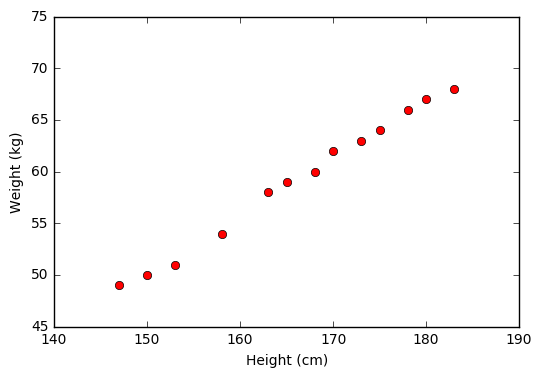
\includegraphics[width=.5\textwidth]{Chapters/03_SimpleML/3_linearregression/output_3_0.png}
%     }
% \end{figure}

Các điểm dữ liệu được minh hoạ bởi các điểm hình tròn trong Hình~\ref{fig:3_2}.
Ta thấy rằng dữ liệu được sắp xếp gần như theo một đường thẳng, vậy mô hình hồi
quy tuyến tính sau đây có khả năng cho kết quả tốt, với \pythoninline{w_0} là
hệ số điều chỉnh $b$:
\begin{center}
(cân nặng) = \pythoninline{w_1}*(chiều cao) + \pythoninline{w_0}
\end{center}


\subsection{Nghiệm theo công thức}

Tiếp theo, ta tìm các hệ số \pythoninline{w_1} và
\pythoninline{w_0} dựa vào công thức~\eqref{eqn:3_finalsolution}. Giả
nghịch đảo của một ma trận \pythoninline{A} trong Python được tính bằng
\pythoninline{numpy.linalg.pinv(A)}.% , \pythoninline{pinv} là từ viết tắt của
% \textit{pseudo inverse}.

% \begin{lstlisting}[language=Python]
% # Building Xbar
% one = np.ones((1, X.shape[1]))
% Xbar = np.concatenate((one, X), axis = 0)

% # Calculating weights of the fitting line
% A = np.dot(Xbar, Xbar.T)
% b = np.dot(Xbar, y)
% w = np.dot(np.linalg.pinv(A), b)
% # Preparing the fitting line
% w_0 = w[0][0]
% w_1 = w[1][0]
% x0 = np.linspace(145, 185, 2, endpoint=True)
% y0 = w_0 + w_1*x0

% # Drawing the fitting line
% plt.plot(X, y.T, 'ro')     # data
% plt.plot(x0, y0)           # the fitting line
% plt.axis([140, 190, 45, 75]) # xmin, xmax, ymin, ymax
% plt.xlabel('Height (cm)')
% plt.ylabel('Weight (kg)')
% plt.show()
% \end{lstlisting}

\begin{lstlisting}[language=Python]
# Building Xbar
one = np.ones((X.shape[0], 1))
Xbar = np.concatenate((one, X), axis = 1) # each row is one data point
# Calculating weights of the linear regression model
A = np.dot(Xbar.T, Xbar)
b = np.dot(Xbar.T, y)
w = np.dot(np.linalg.pinv(A), b)
# weights
w_0, w_1 = w[0], w[1]
\end{lstlisting}

% Kết quả hiển thị:
% \begin{lstlisting}[language=Python]
% w =  [[-33.73541021]
%  [  0.55920496]]
% \end{lstlisting}


% <div class="imgcap">
% <img src ="/assets/LR/output_5_1.png" align = "center">
% </div>

\begin{figure}[t]
% caption on side
\floatbox[{\capbeside\thisfloatsetup{capbesideposition={right,top},capbesidewidth=5.5cm}}]{figure}[\FBwidth]
{\caption{
Minh hoạ dữ liệu và đường thẳng xấp xỉ tìm được bởi hồi quy tuyến tính
}
\label{fig:3_2}}
{ % figure here
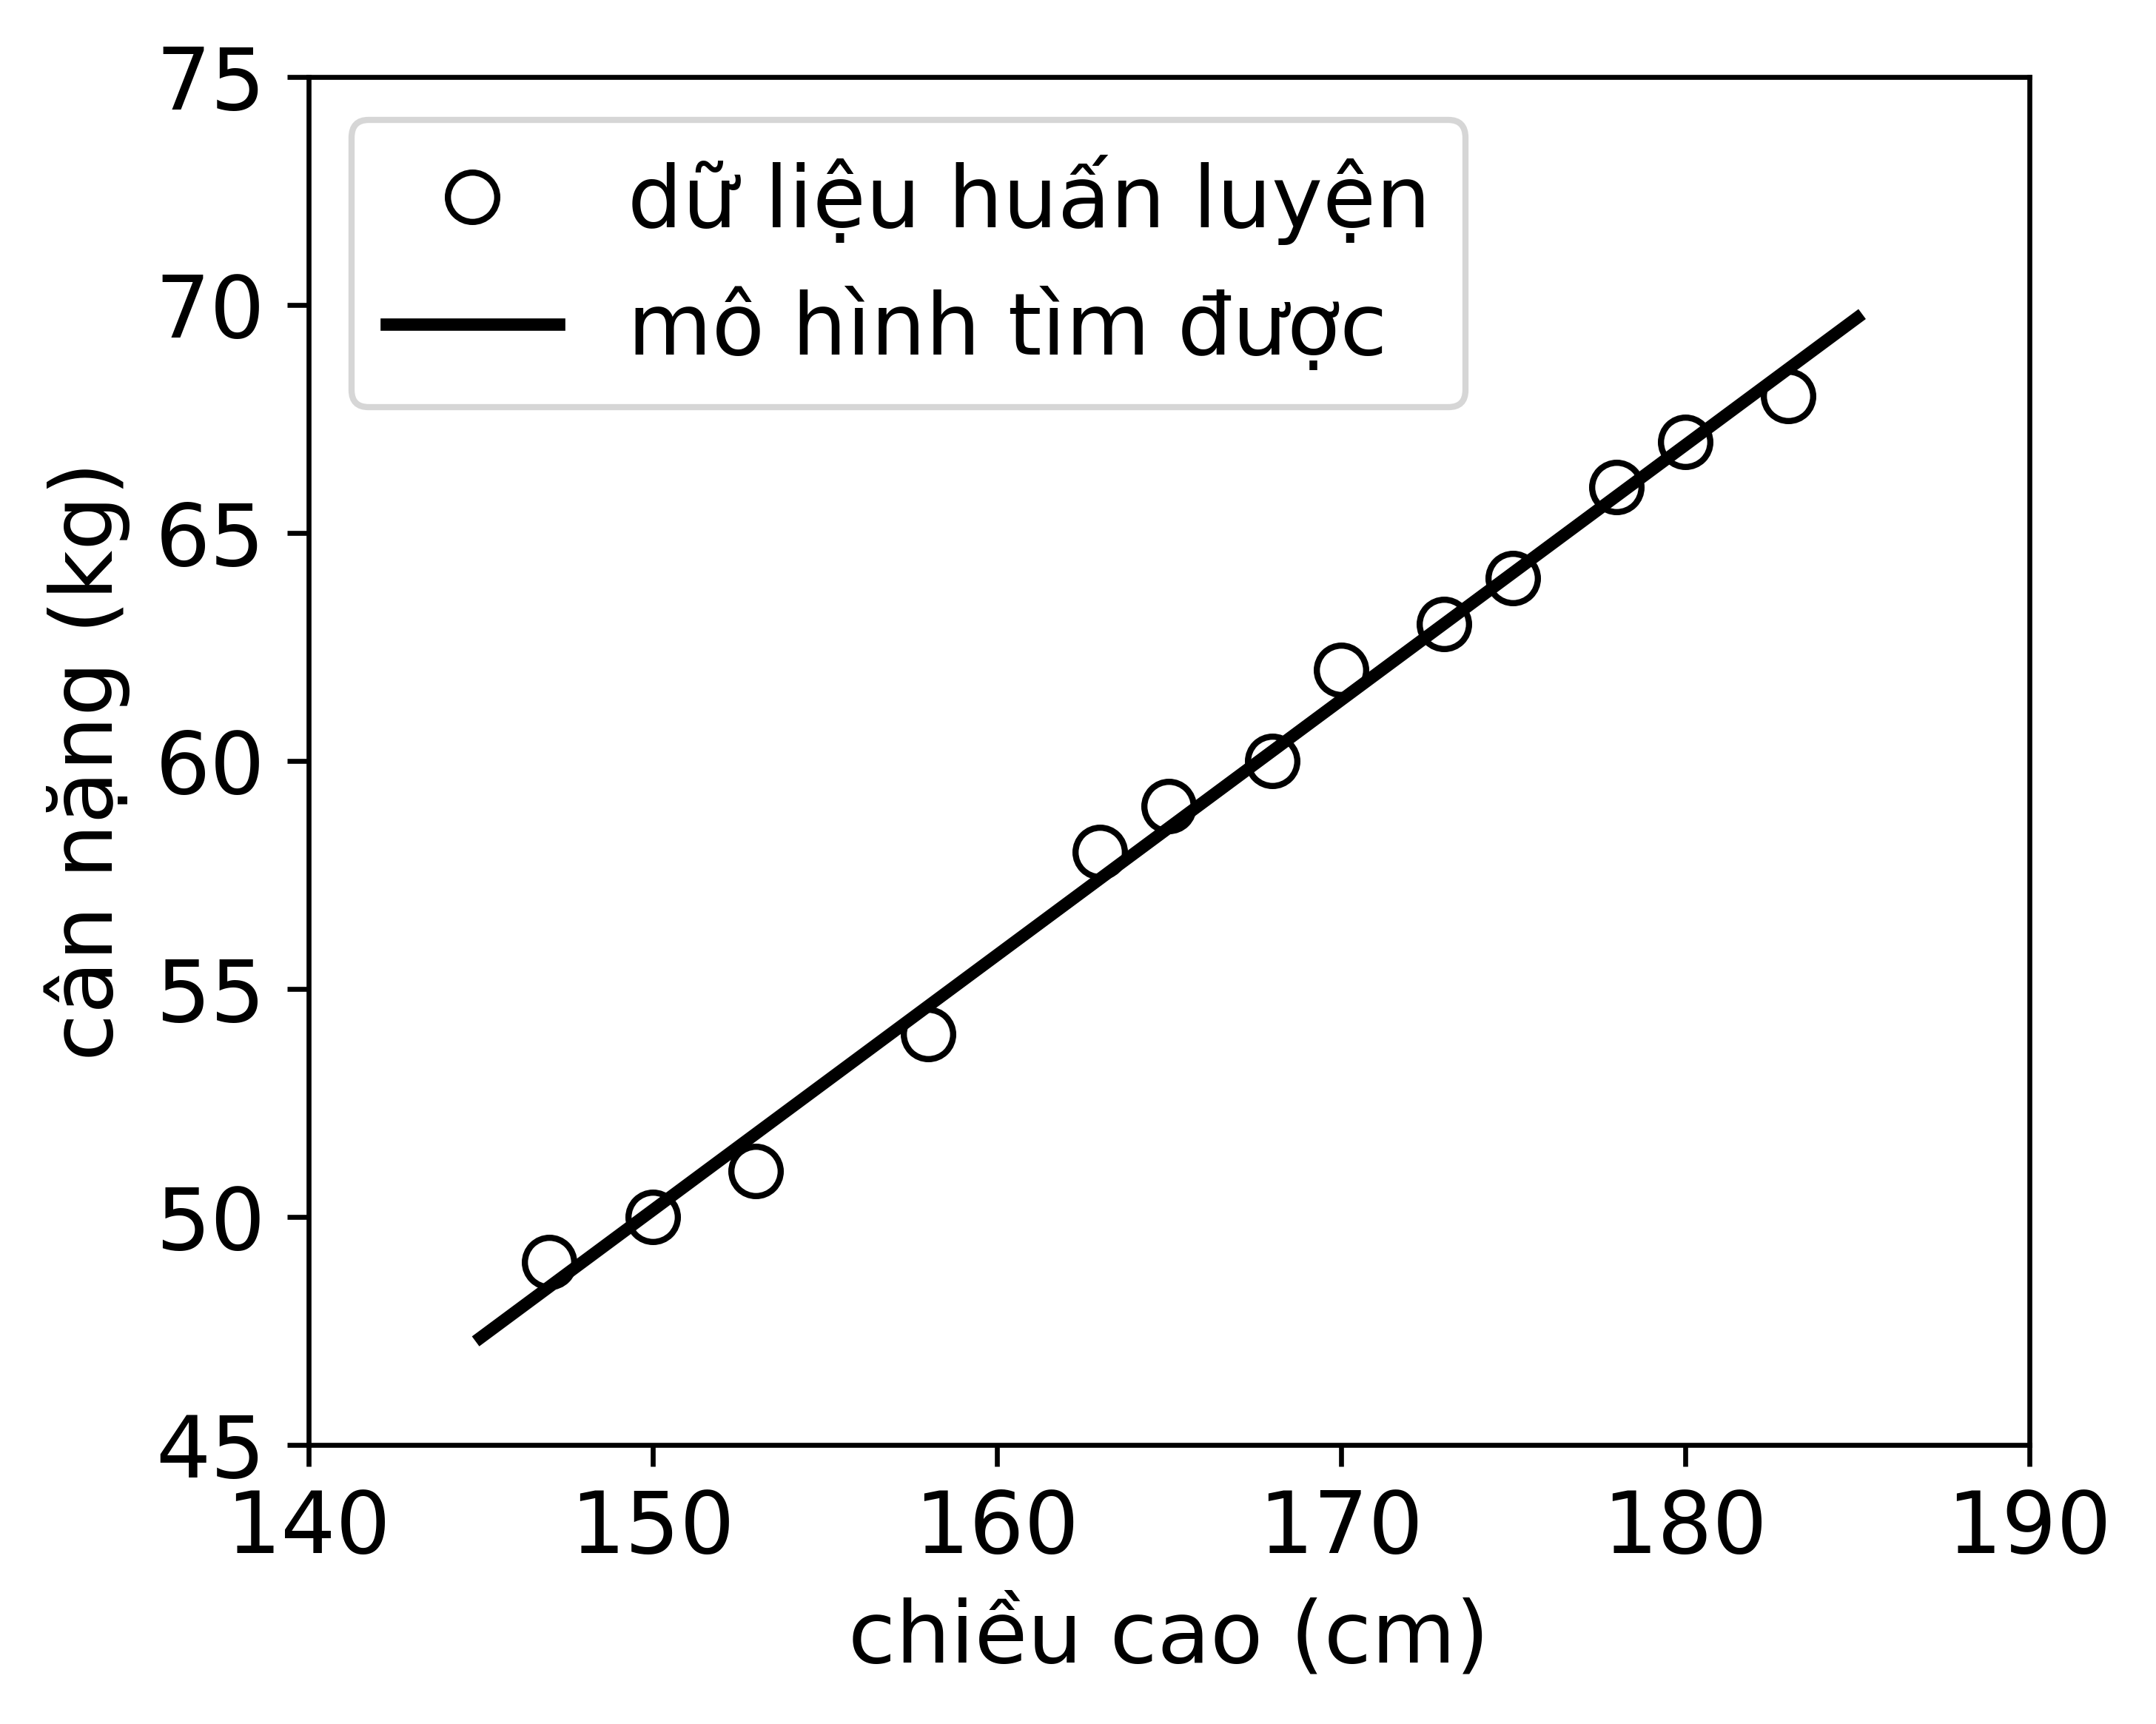
\includegraphics[width=.5\textwidth]{Chapters/03_SimpleML/3_linearregression/lr_ex.png}
}
\end{figure}
Đường thẳng mô tả mối quan hệ giữa đầu vào và đầu ra được minh hoạ trong
Hình~\ref{fig:3_2}. Ta thấy rằng các điểm dữ liệu nằm khá gần đường thẳng dự
đoán. Vậy mô hình hồi quy tuyến tính hoạt động tốt với tập dữ liệu huấn luyện.
Bây giờ, chúng ta sử dụng mô hình này để dự đoán dữ liệu trong tập kiểm tra.

\begin{lstlisting}[language=Python]
y1 = w_1*155 + w_0
y2 = w_1*160 + w_0
print('Input 155cm, true output 52kg, predicted output %.2fkg.'  %(y1) )
print('Input 160cm, true output 56kg, predicted output %.2fkg.'  %(y2) )
\end{lstlisting}
Kết quả:
\begin{lstlisting}
Input 155cm, true output 52kg, predicted output 52.94kg.
Input 160cm, true output 56kg, predicted output 55.74kg.
\end{lstlisting}

Chúng ta thấy rằng đầu ra dự đoán khá gần đầu ra thực sự.


\subsection{Nghiệm theo thư viện scikit-learn}

Tiếp theo, chúng ta sẽ sử dụng thư viện scikit-learn để tìm nghiệm.

\begin{lstlisting}[language=Python]
from sklearn import datasets, linear_model
# fit the model by Linear Regression
regr = linear_model.LinearRegression()
regr.fit(X, y) # in scikit-learn, each sample is one row
# Compare two results
print("scikit-learn's solution: w_1 = ", regr.coef_[0], "w_0 = ",\
      regr.intercept_)
print("our solution           : w_1 = ", w[1], "w_0 = ", w[0])
\end{lstlisting}
% \newpage
Kết quả:
\begin{lstlisting}[language=Python]
scikit-learn solution: w_1 =  [ 0.55920496] w_0 =  [-33.73541021]
our solution         : w_1 =  [ 0.55920496] w_0 =  [-33.73541021]
\end{lstlisting}

Chúng ta thấy rằng hai kết quả thu được là như nhau.


\section{Thảo luận}


\subsection{Các bài toán có thể giải bằng hồi quy tuyến tính}
\index{hồi quy đa thức -- polynomial regression}
\index{polynomial regression -- hồi quy đa thức}
Hàm số $y \approx f(\bx)= \bx^T\bw + b$ là một hàm tuyến tính
theo cả $ \bw$ và $\bx$. Hồi quy tuyến tính có thể áp
dụng cho các mô hình chỉ cần tuyến tính theo $\bw$. Ví dụ
\begin{equation}
y \approx w_1 x_1 + w_2 x_2 + w_3 x_1^2 +w_4 \sin(x_2) + w_5 x_1x_2 + w_0
\end{equation}
là một hàm tuyến tính theo $\bw$ nhưng không tuyến tính theo $\bx$. Bài toán này vẫn có thể được giải bằng
hồi quy tuyến tính. Với mỗi vector đặc trưng $\bx=[x_1, x_2]^T $, ta
tính vector đặc trưng mới $\tilde{\bx} = [x_1, x_2, x_1^2,
\sin(x_2), x_1x_2]^T$ rồi áp dụng hồi quy tuyến tính với dữ liệu mới này. Tuy
nhiên, việc tìm ra các hàm số $\sin(x_2)$ hay $x_1x_2$ là tương đối
{không tự nhiên}. \textit{Hồi quy đa thức} (polynomial regression) thường được sử dụng nhiều hơn với các vector đặc trưng mới có dạng
$[1, x_1, x_1^2, \dots]^T$. Một ví dụ về hồi quy đa thức bậc 3 được thể hiện
trong Hình~\ref{fig:3_lra}.

% \begin{figure}[t]
%     % caption on side
%     \floatbox[{\capbeside\thisfloatsetup{capbesideposition={right,top},capbesidewidth=6cm}}]{figure}[\FBwidth]
%     {\caption{
%     Polynomial regression bậc ba.
%     }
%     \label{fig:3_polyreg}}
%     { % figure here
%     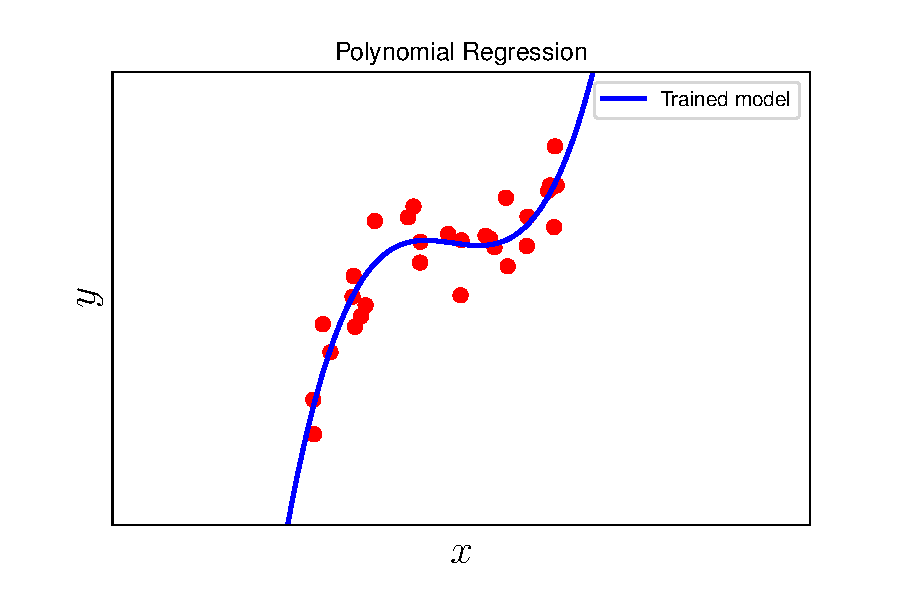
\includegraphics[width=.55\textwidth]{ebookML_src/src/linear_regression/polyregression.pdf}
%     }
% \end{figure}

%% *****************************************************************************
\begin{figure}[t]
\begin{subfigure}{0.49\textwidth}
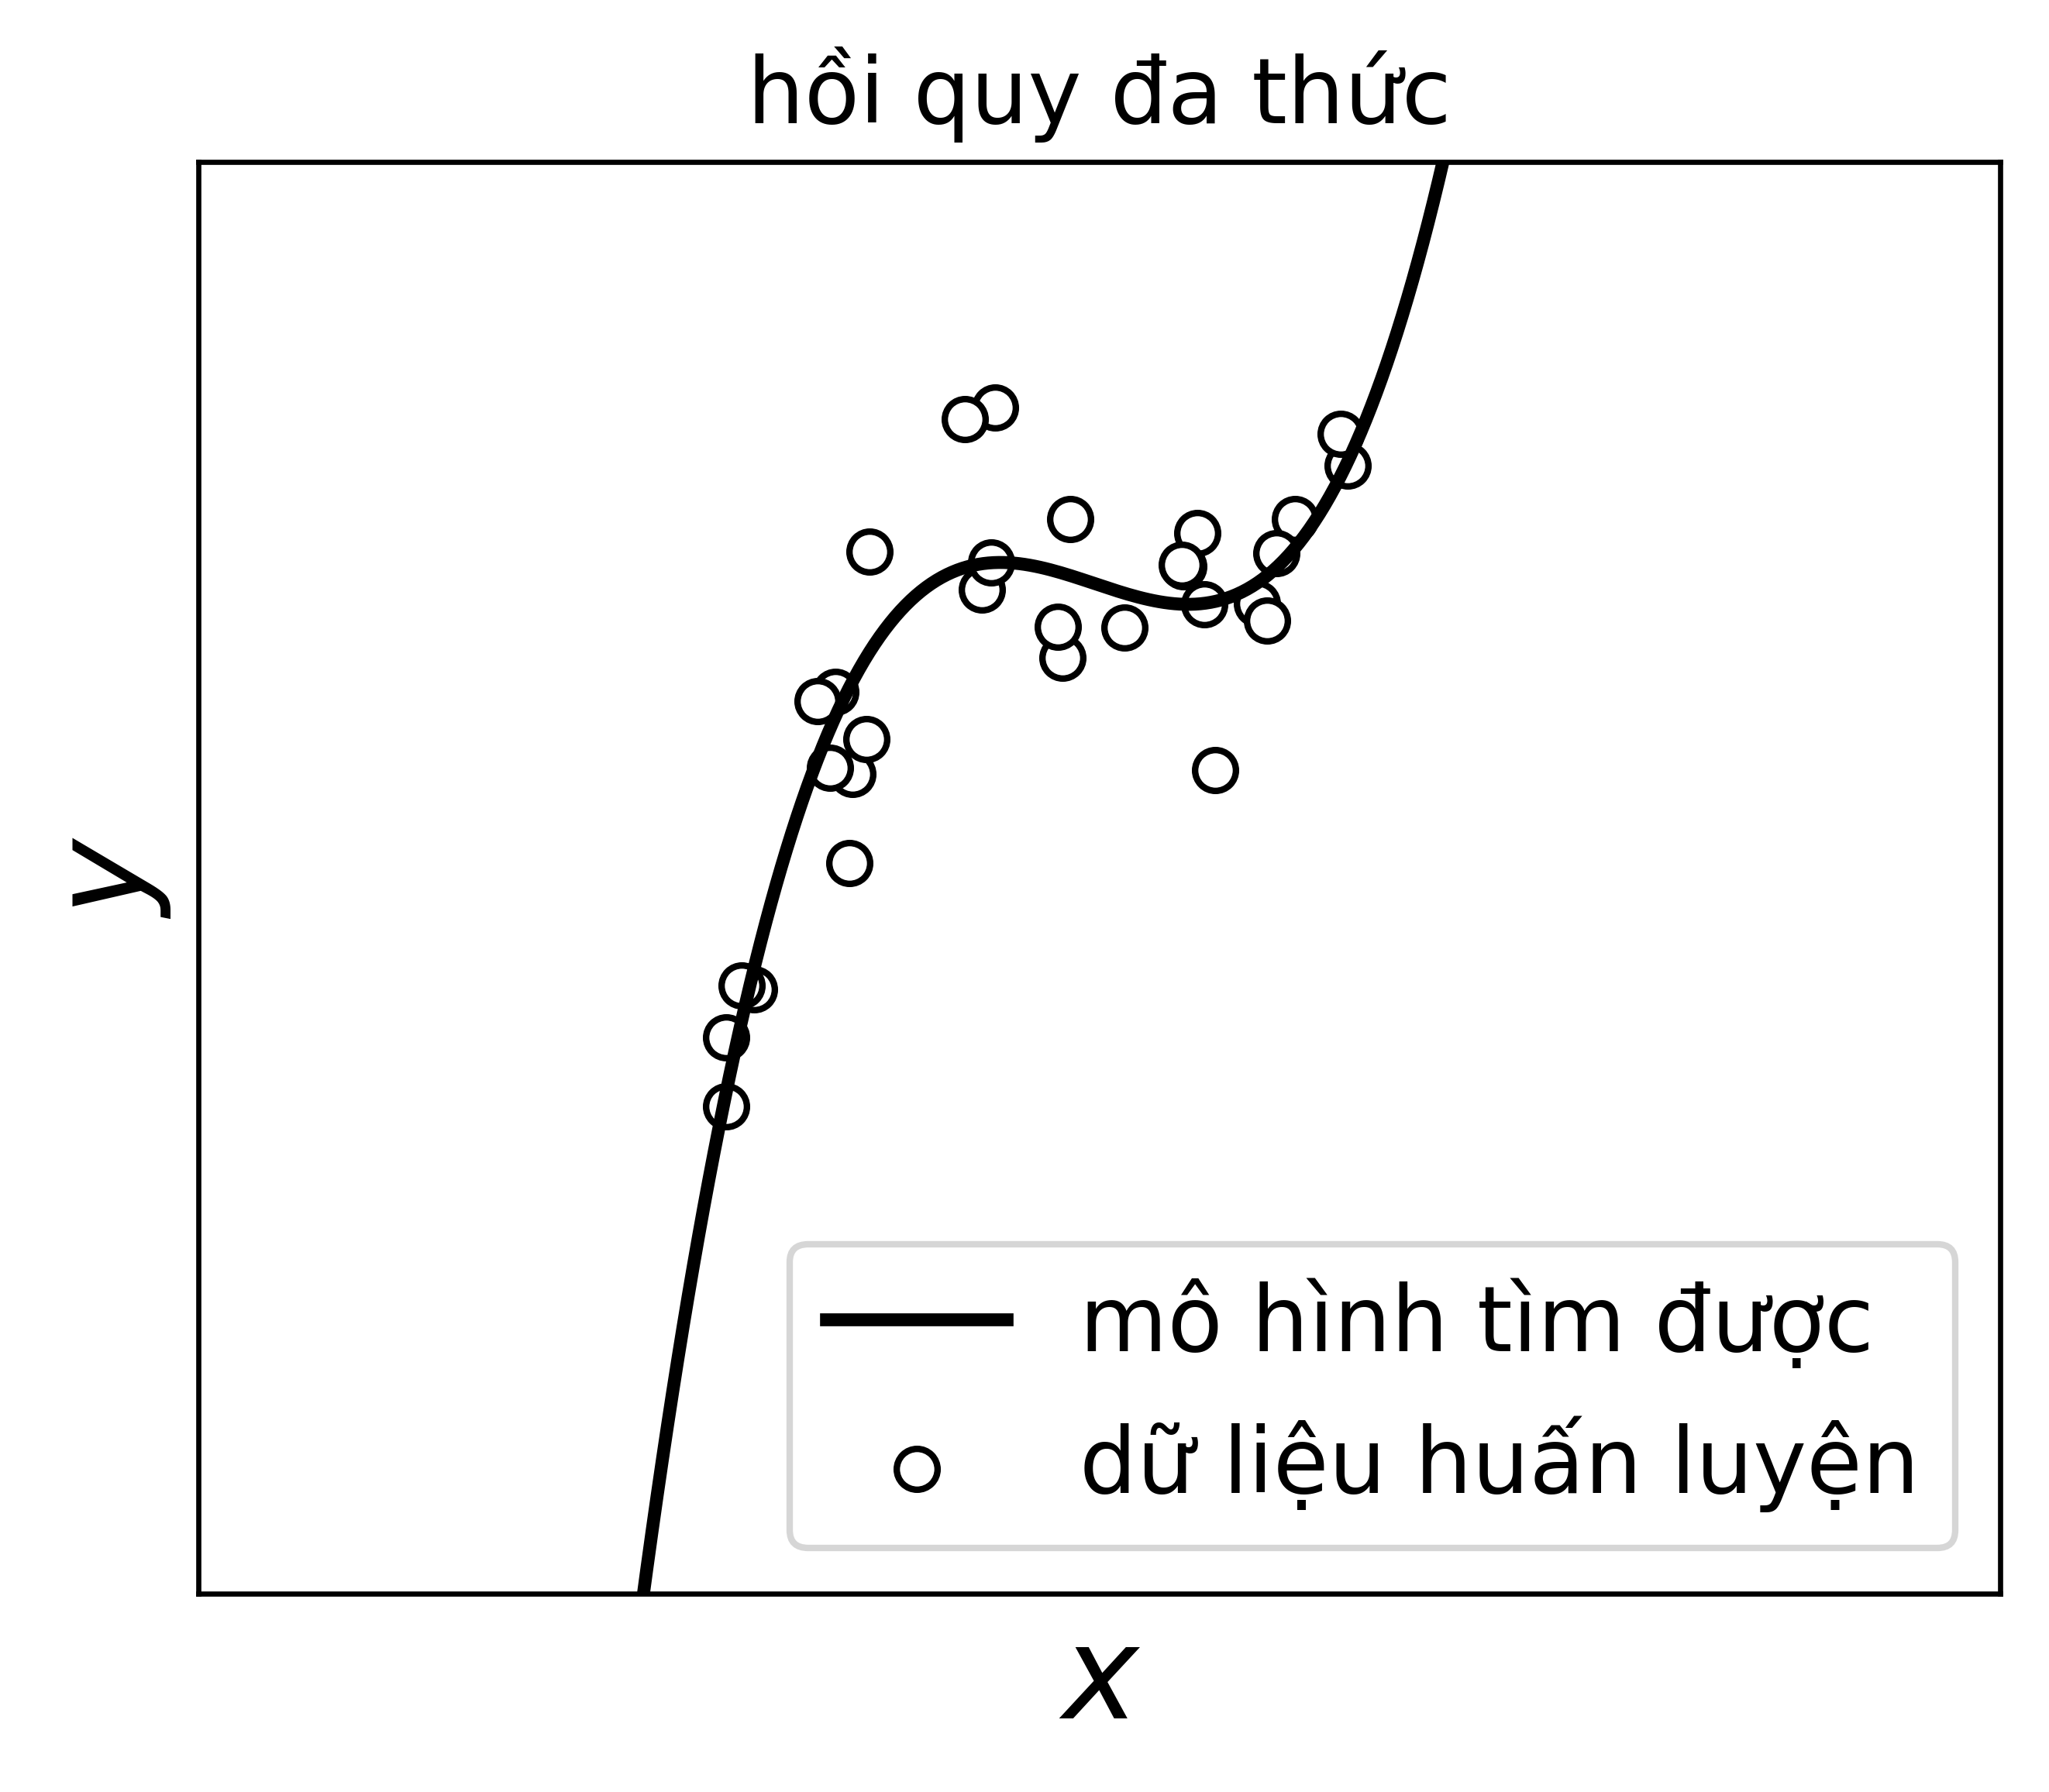
\includegraphics[width=0.99\linewidth]{Chapters/03_SimpleML/3_linearregression/polyreg.png}
\caption{}
\label{fig:3_lra}
\end{subfigure}
\begin{subfigure}{0.49\textwidth}
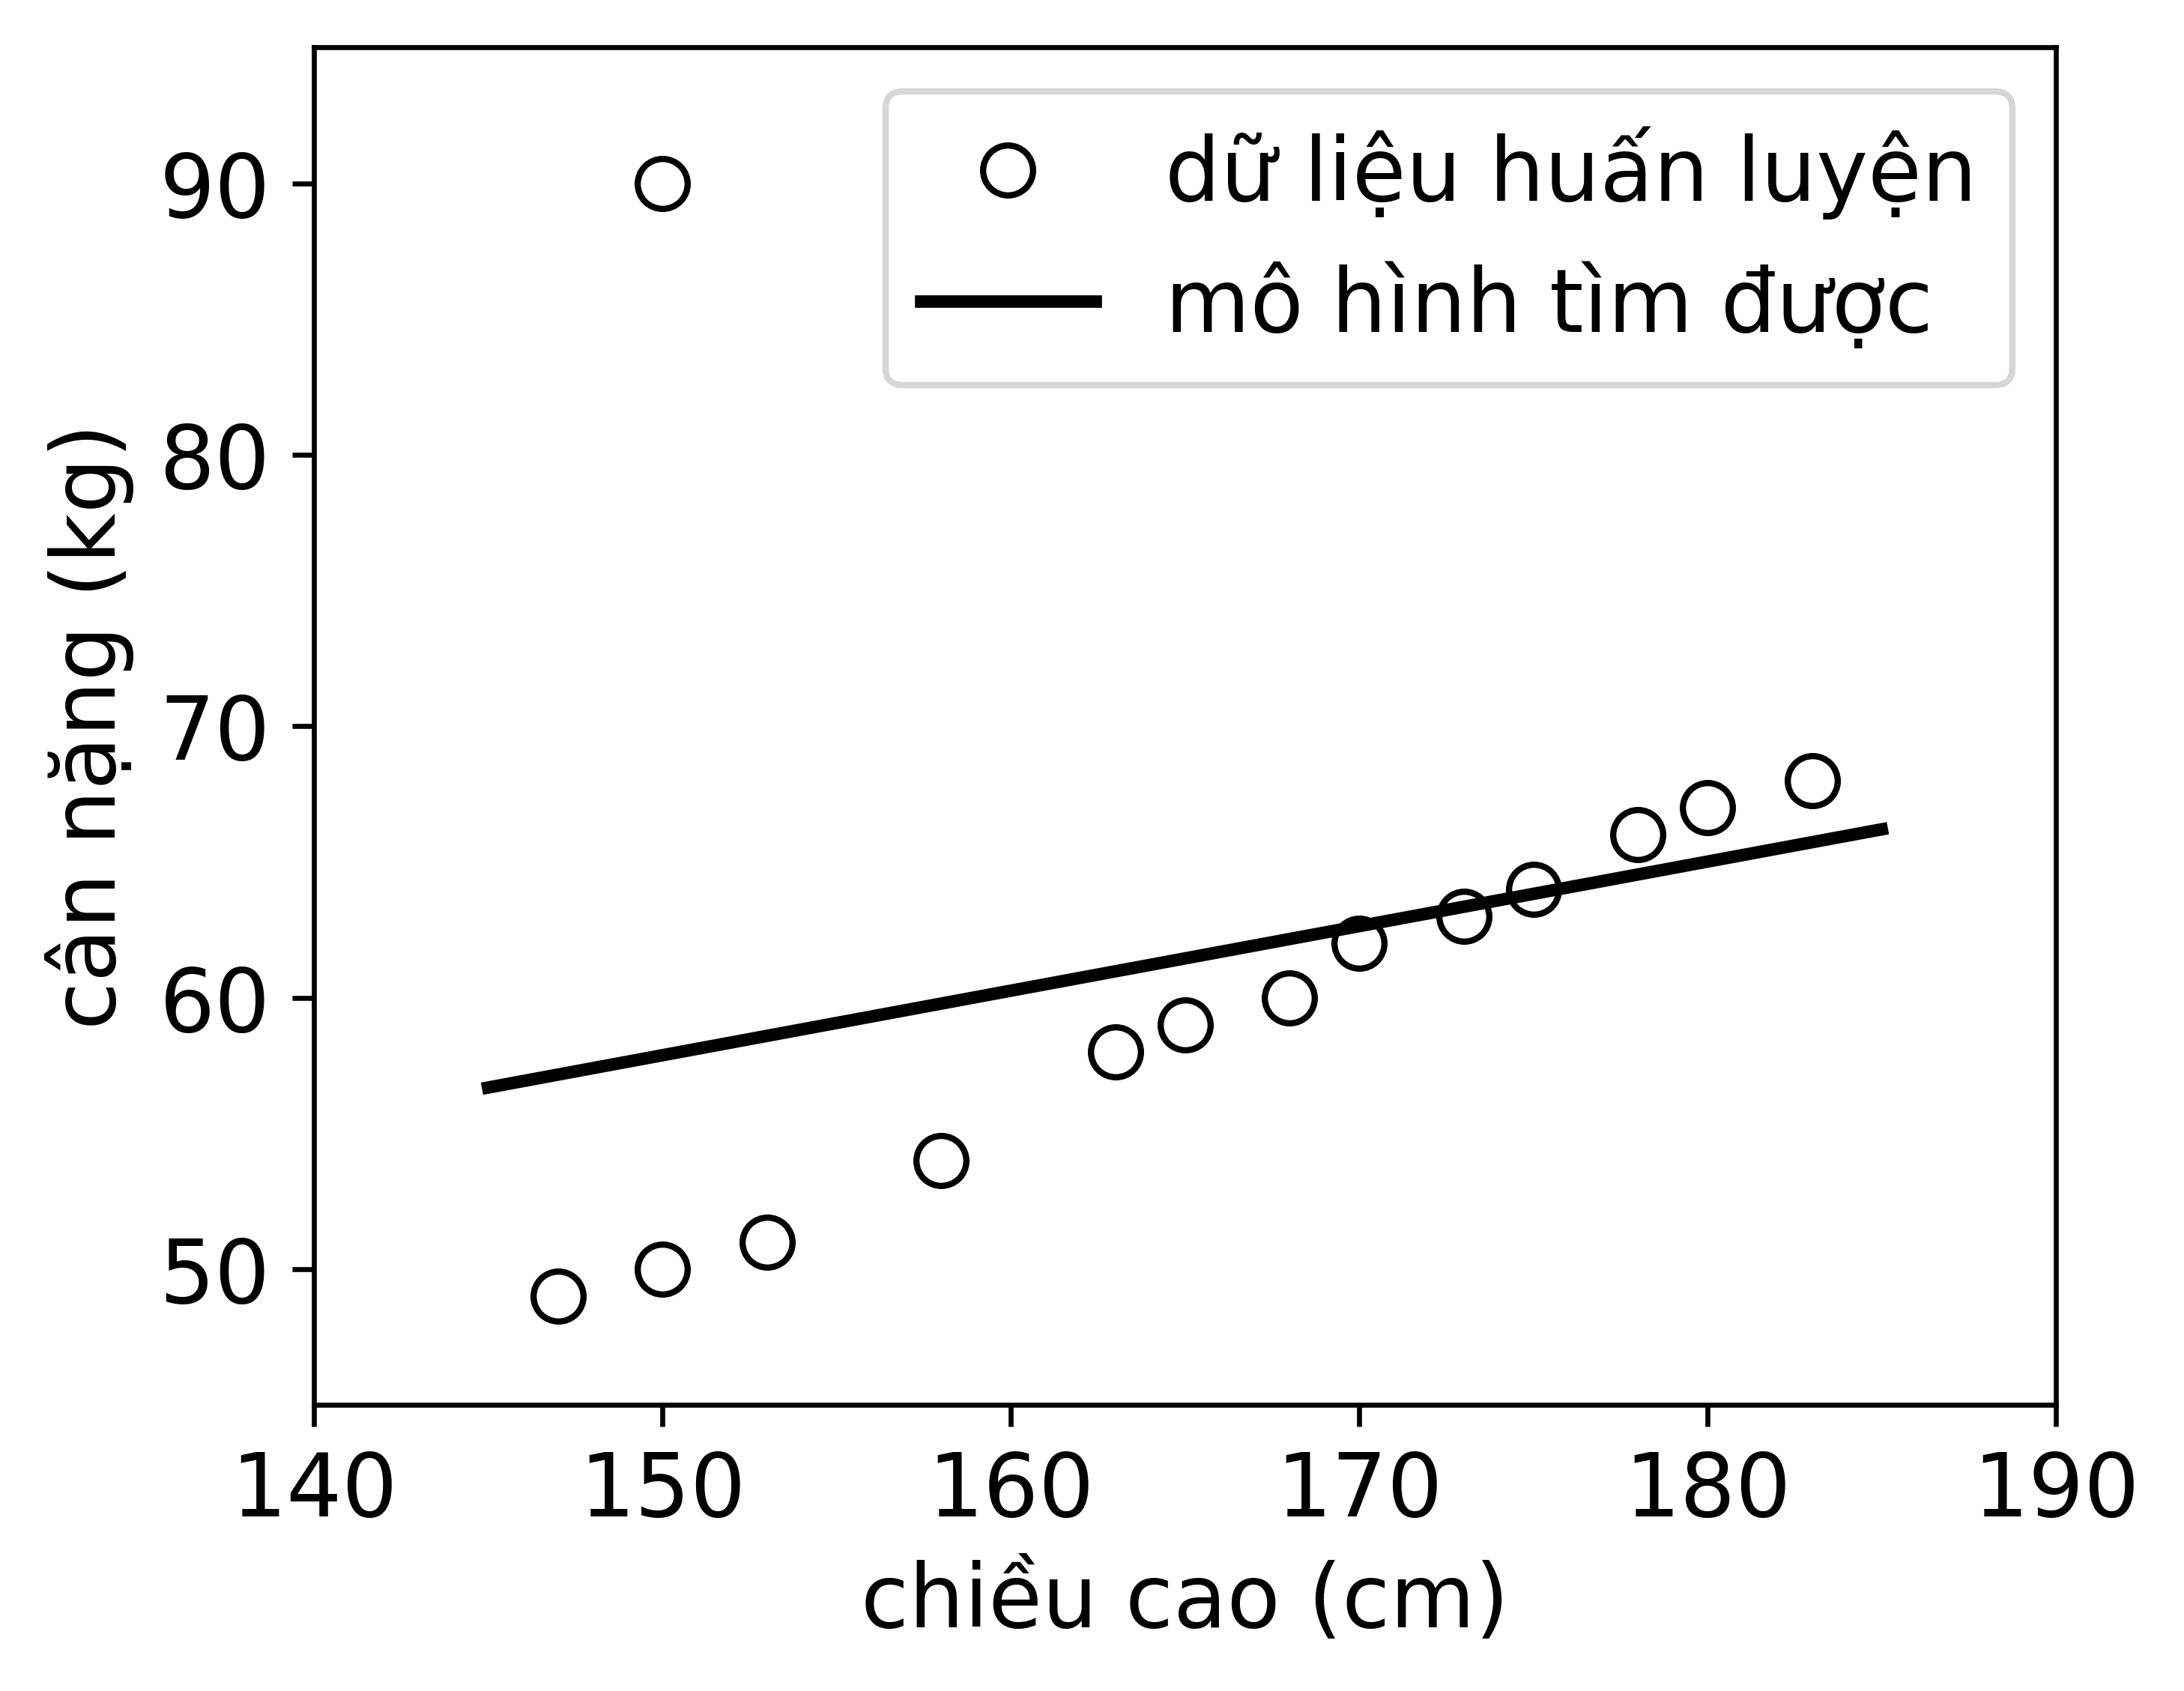
\includegraphics[width=0.99\linewidth]{ebookML_src/src/linear_regression/noise.png}
\caption{}
\label{fig:3_lrb}
\end{subfigure}
\caption{ (a) Hồi quy đa thức bậc ba (b) Hồi quy tuyến tính nhạy cảm với nhiễu.
}
\label{fig:3_lr}
\end{figure}
%% *****************************************************************************



\subsection{Hạn chế của hồi quy tuyến tính}

Hạn chế đầu tiên của hồi quy tuyến tính là nó rất \textit{nhạy cảm với nhiễu} (sensitive to noise). Trong ví dụ về mối quan hệ giữa chiều cao và cân
nặng bên trên, nếu có chỉ một cặp dữ liệu {nhiễu} (150 cm, 90kg) thì kết
quả sẽ sai khác đi rất nhiều (xem Hình~\ref{fig:3_lrb}).
% \begin{figure}[t]
%     % caption on side
%     \floatbox[{\capbeside\thisfloatsetup{capbesideposition={right,top},capbesidewidth=6cm}}]{figure}[\FBwidth]
%     {\caption{
%     Linear regression hoạt động không tốt khi có nhiễu.
%     }
%     \label{fig:3_withnoise}}
%     { % figure here
%     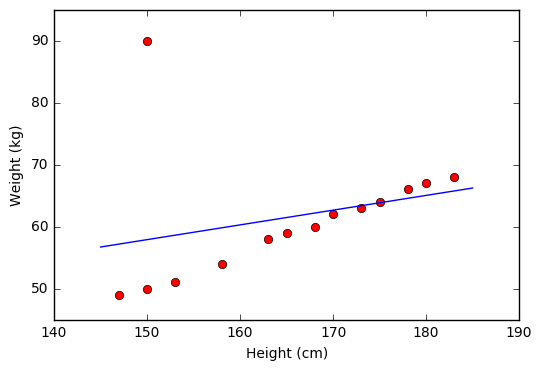
\includegraphics[width=.5\textwidth]{Chapters/03_SimpleML/3_linearregression/output_13_1.png}
%     }
% \end{figure}

\index{hồi quy Huber -- Huber regression}
\index{Huber regression -- hồi quy Huber}

Một kỹ thuật giúp tránh hiện tượng này là loại bỏ các nhiễu trong quá trình tìm nghiệm. Việc làm này có thể phức tạp và tương đối tốn thời gian. Có một cách khác giúp tránh công việc loại bỏ nhiễu là sử dụng \textit{mất mát Huber}\footnote{Huber loss (\url{https://goo.gl/TBUWzg})}. Hồi quy tuyến tính với mất mát Huber được gọi là \textit{hồi quy Huber}, được khẳng định là có khả năng kháng nhiễu tốt hơn. Xem thêm \textit{Huber Regressor, scikit learn} (\url{https://goo.gl/h2rKu5}).

Hạn chế thứ hai của hồi quy tuyến tính là nó \textit{không biễu diễn được các mô
hình phức tạp}. Mặc dù phương pháp này có thể được áp dụng nếu quan
hệ giữa đầu ra và đầu vào là phi tuyến, mối quan hệ này vẫn đơn giản hơn
nhiều so với các mô hình thực tế. Hơn nữa, việc tìm ra các đặc trưng $x_1^2,
\sin(x_2), x_1x_2$ như trên là không khả thi khi số chiều dữ liệu lớn lên.


\subsection{Hồi quy ridge}
\index{hồi quy ridge -- ridge regression}
\index{ridge regression -- hồi quy ridge}

Có một kỹ thuật nhỏ giúp tránh trường hợp $\bX\bX^T$ không khả nghịch là biến nó thành $\bA = \bX\bX^T + \lambda\bI$ với $\lambda$ là một số dương nhỏ
và $\bI$ là ma trận đơn vị với bậc phù hợp.

Ma trận $\bA$ là khả nghịch vì nó là một ma trận xác định dương. Thật vậy, với
mọi $\bw \neq \bzero$,
\begin{equation*}
\bw^T\bA\bw = \bw^T(\bX\bX^T + \lambda \bI) \bw = \bw^T\bX\bX^T\bw  +
\lambda \bw^T\bw = \|\bX^T\bw\|_2^2 + \lambda \|\bw\|_2^2 > 0.
\end{equation*}
Lúc này, nghiệm của bài toán là $\by = (\bX \bX^T + \lambda \bI)^{-1} \bX\by$.

Xét hàm mất mát
\begin{equation}
\label{eqn:3_ridge}
\L_2(\bw) = \frac{1}{2N}(\|\by - \bX^T\bw\|_2^2 + \lambda\|\bw\|_2^2).
\end{equation}
Phương trình gradient theo $\bw$ bằng không:
\begin{equation}
\frac{\nabla \L_2(\bw)}{\nabla \bw} = \bzero \Leftrightarrow
\frac{1}{N}(\bX(\bX^T\bw - \by) + \lambda \bw) = \bzero \Leftrightarrow
(\bX\bX^T + \lambda \bI) \bw = \bX\by
\end{equation}
Ta thấy $\bw = (\bX\bX^T + \lambda\bI)^{-1}\bX\by$ chính là nghiệm của
bài toán tối thiểu $\L_2(\bw)$ trong~\eqref{eqn:3_ridge}. Mô hình machine learning với hàm mất mát~\eqref{eqn:3_ridge} còn được
gọi là \textit{hồi quy ridge}.
Ngoài việc giúp phương trình gradient theo hệ số bằng không có nghiệm duy
nhất, hồi quy ridge còn giúp mô hình tránh được overfitting như sẽ thấy trong Chương~\ref{cha:overfitting}.

\subsection{Phương pháp tối ưu khác}


Hồi quy tuyến tính là một mô hình đơn giản, lời giải cho phương trình gradient
bằng không cũng không phức tạp. {Trong hầu hết các trường hợp, việc giải các
phương trình gradient bằng không tương đối phức tạp.} Tuy nhiên, nếu ta tính được đạo hàm của hàm mất mát, các tham số mô hình có thể được giải bằng một phương pháp hữu dụng có tên \textit{gradient descent}. Trên thực tế, một vector đặc trưng có thể
có kích thước rất lớn, dẫn đến ma trận $\bX\bX^T$ cũng có kích thước lớn và việc
tính ma trận nghịch đảo có thể không lợi về mặt tính toán. Gradient descent sẽ
giúp tránh được việc tính ma trận nghịch đảo. Chúng ta sẽ hiểu kỹ hơn về phương
pháp này trong Chương~\ref{cha:gradient_descent}.

% \subsection{Đọc thêm}
% \begin{enumerate}
%     \item \textit{Simple Linear Regression Tutorial for Machine Learning} (\url{https://goo.gl/WRVda8}).

%     \item \textit{Regularization: Ridge Regression and the LASSO} (\url{https://goo.gl/uRzN1K}).
% \end{enumerate}


%!TEX root = ../../book_ML.tex
\chapter{Quá khớp}
\label{cha:overfitting}

\index{quá khớp -- overfitting}
\index{overfitting -- quá khớp}

\textit{Quá khớp} (overfitting) là một hiện tượng không mong muốn thường gặp, người xây dựng mô hình
machine learning cần nắm được các kỹ thuật để tránh hiện tượng này.

\section{Giới thiệu}
% \index{tính phổ quágeneralization}

Trong các mô hình học có giám sát, ta thường
phải đi tìm một mô hình ánh xạ các vector đặc trưng thành các kết quả tương ứng
trong tập huấn luyện. Nói cách khác, ta cần đi tìm hàm số $f$ sao cho $y_i \approx f(\bx_i),
~\forall i = 1, 2,
\dots, N$. Một cách tự nhiên, ta sẽ đi tìm các tham số mô hình của $f$ sao cho
việc xấp xỉ có sai số càng nhỏ càng tốt. Điều này nghĩa là mô hình càng
\textit{khớp} với dữ liệu càng tốt. Tuy nhiên, sự thật là nếu một mô hình {quá
khớp} với dữ liệu huấn luyện thì nó sẽ gây phản tác dụng. Quá khớp là một hiện tượng không mong muốn mà người xây dựng mô hình machine learning cần lưu ý.
Hiện tượng này xảy ra khi mô hình tìm được mang lại kết quả cao trên tập huấn
luyện nhưng không có kết quả tốt trên tập kiểm tra. Nói cách khác, mô hình tìm được không có tính tổng quát.

Để có cái nhìn đầu tiên về quá khớp, chúng ta cùng xem ví dụ trong
Hình~\ref{fig:15_polyreg}. Có 50 cặp điểm dữ liệu ở đó đầu ra là một đa thức bậc
ba của đầu vào cộng thêm nhiễu. Tập dữ liệu này được chia làm hai phần: tập huấn luyện gồm 30 điểm
dữ liệu hình tròn, tập kiểm tra gồm 20 điểm dữ liệu hình vuông. Đồ thị của đa thức bậc ba này được cho bởi đường nét đứt. Bài toán đặt ra là hãy tìm
một mô hình tốt để mô tả quan hệ giữa đầu vào và đầu ra của dữ liệu đã cho. Giả sử thêm rằng đầu ra xấp xỉ là một đa thức của đầu vào.


Với $N$ cặp điểm dữ liệu $(x_1, y_1), \dots, (x_N, y_N)$ với các $x_i$ khác nhau
đôi một, luôn tìm được một {đa thức nội suy Lagrange} $P(x)$ bậc không
vượt quá $N-1$ sao cho $P(x_i) = y_i, ~\forall i = 1, 2, \dots, N$.


\begin{figure}[t]
\begin{subfigure}{0.49\textwidth}
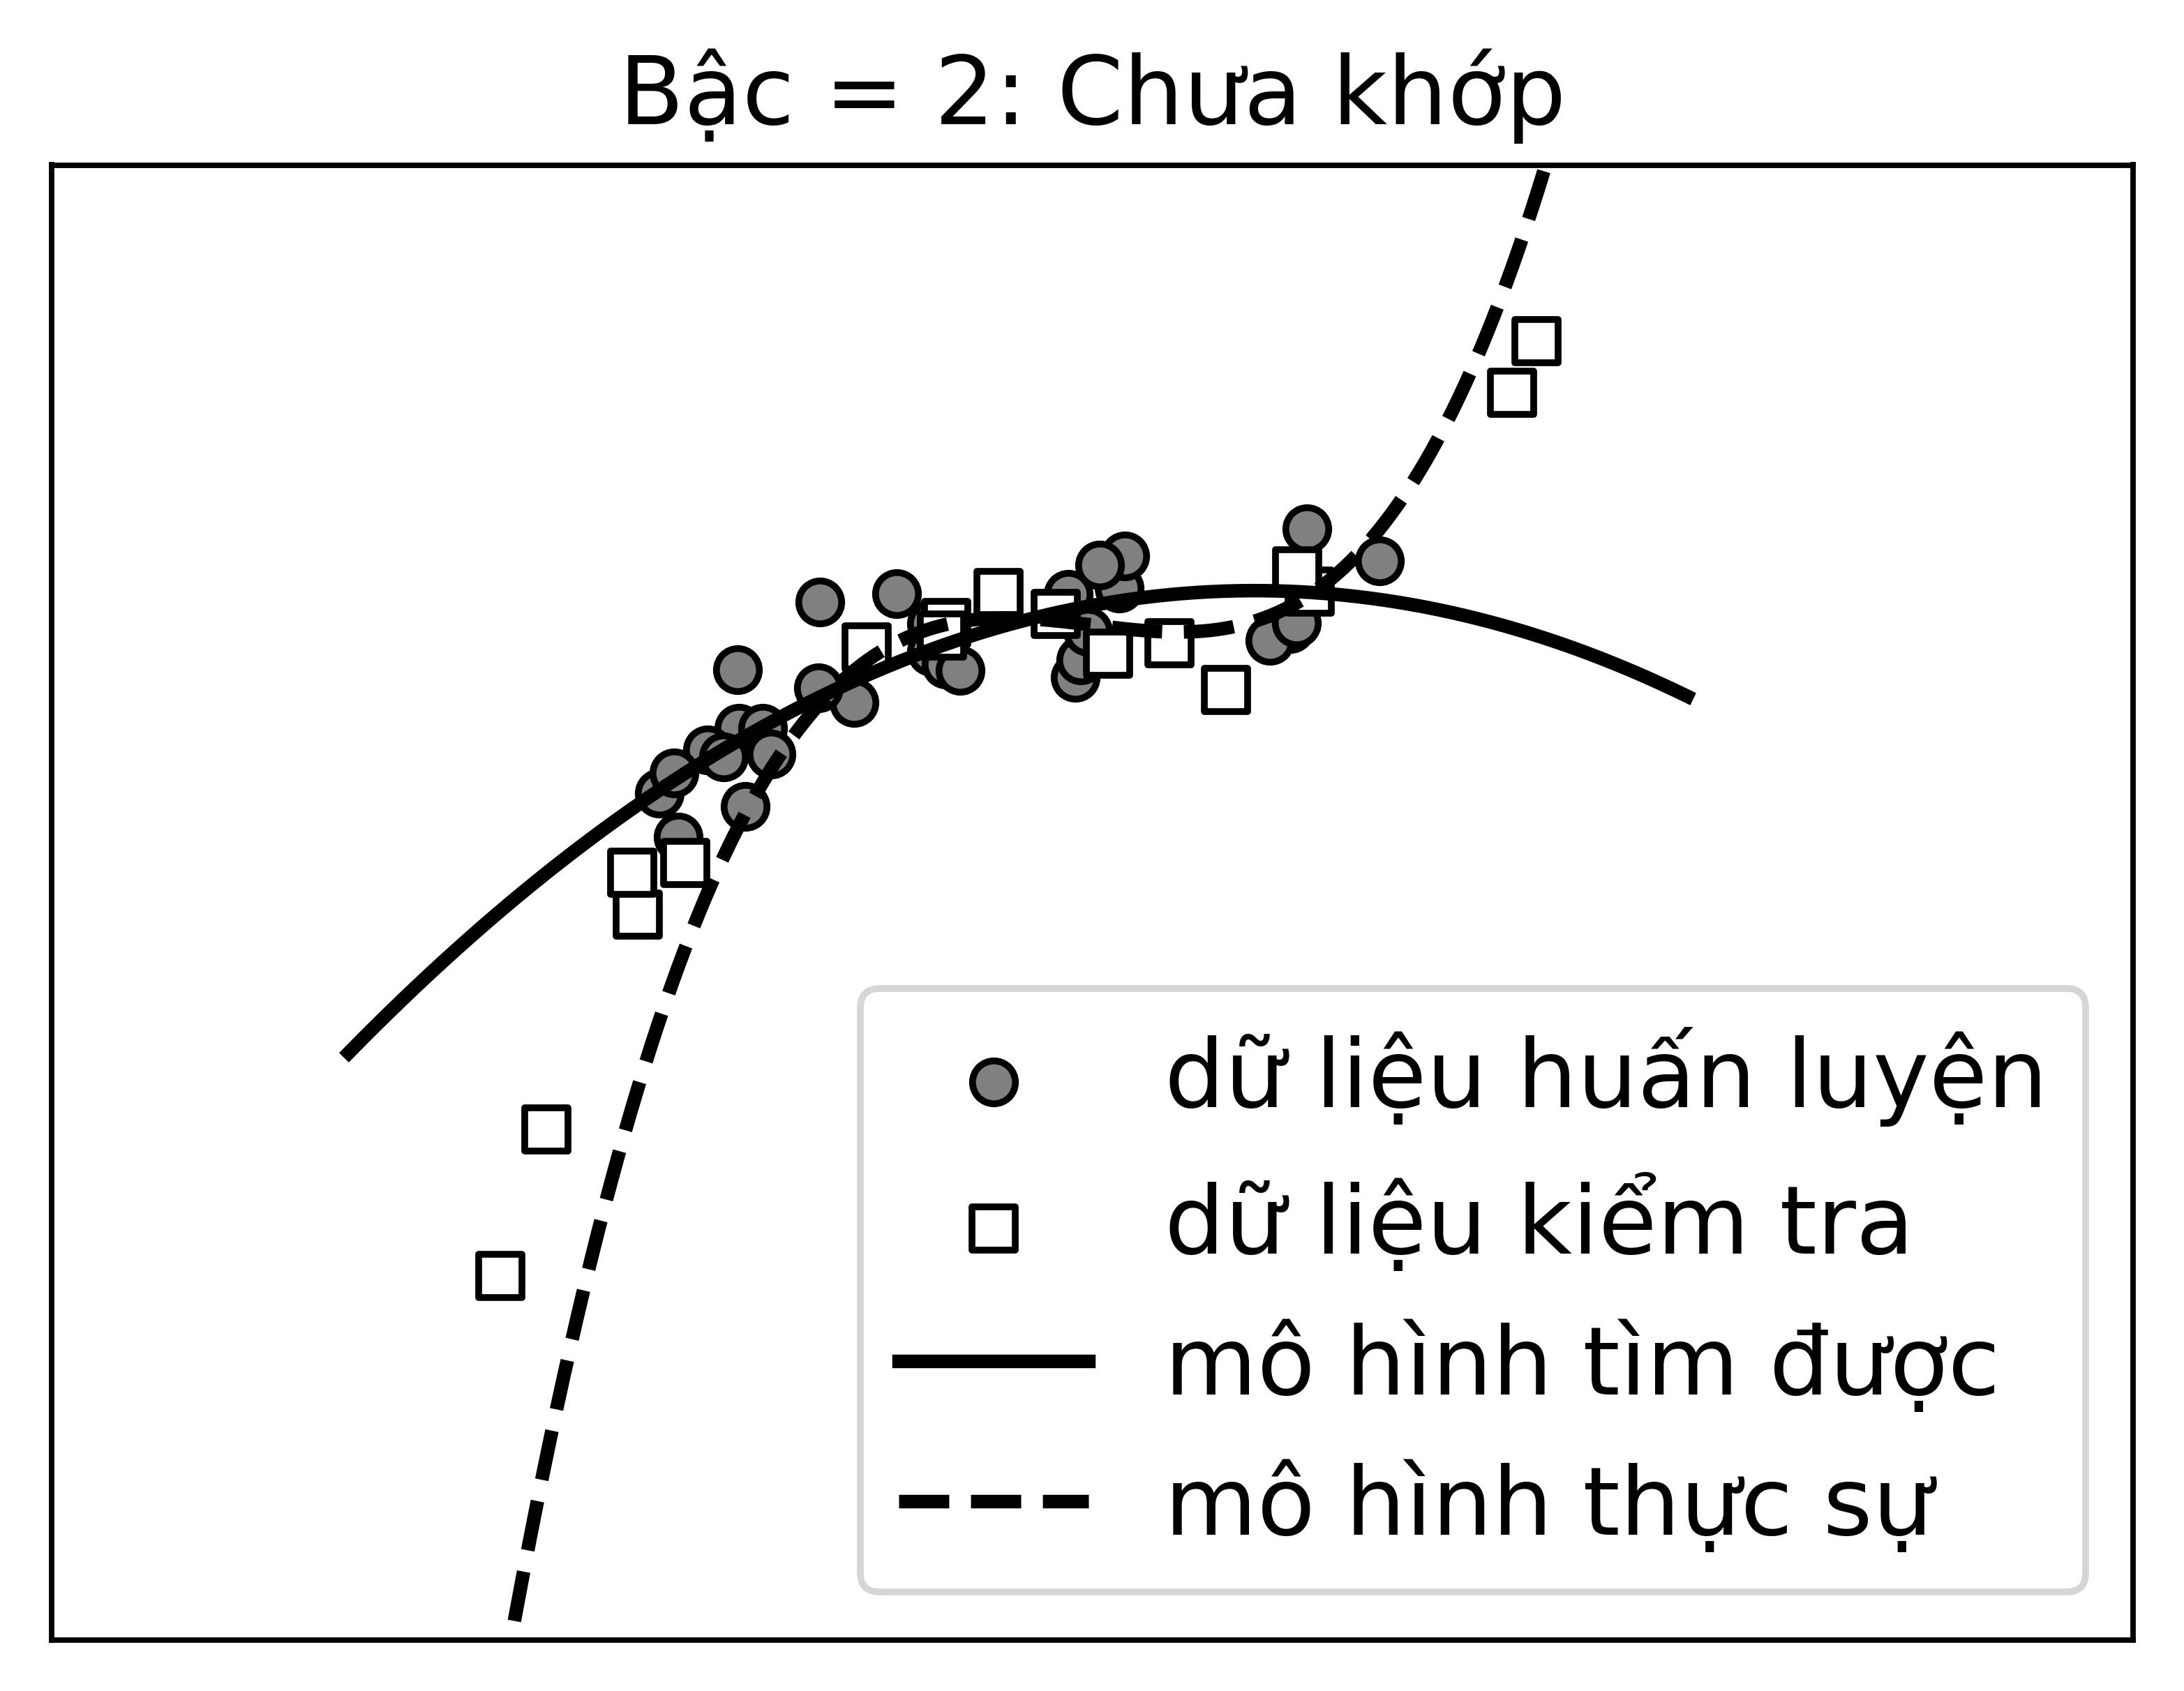
\includegraphics[width=0.99\linewidth]{ebookML_src/src/overfitting/poly2.png}
% {Chapters/01_Overview/15_overfitting/linreg_2.png}
\caption{}
\label{fig:15_polyrega}
\end{subfigure}
\begin{subfigure}{0.49\textwidth}
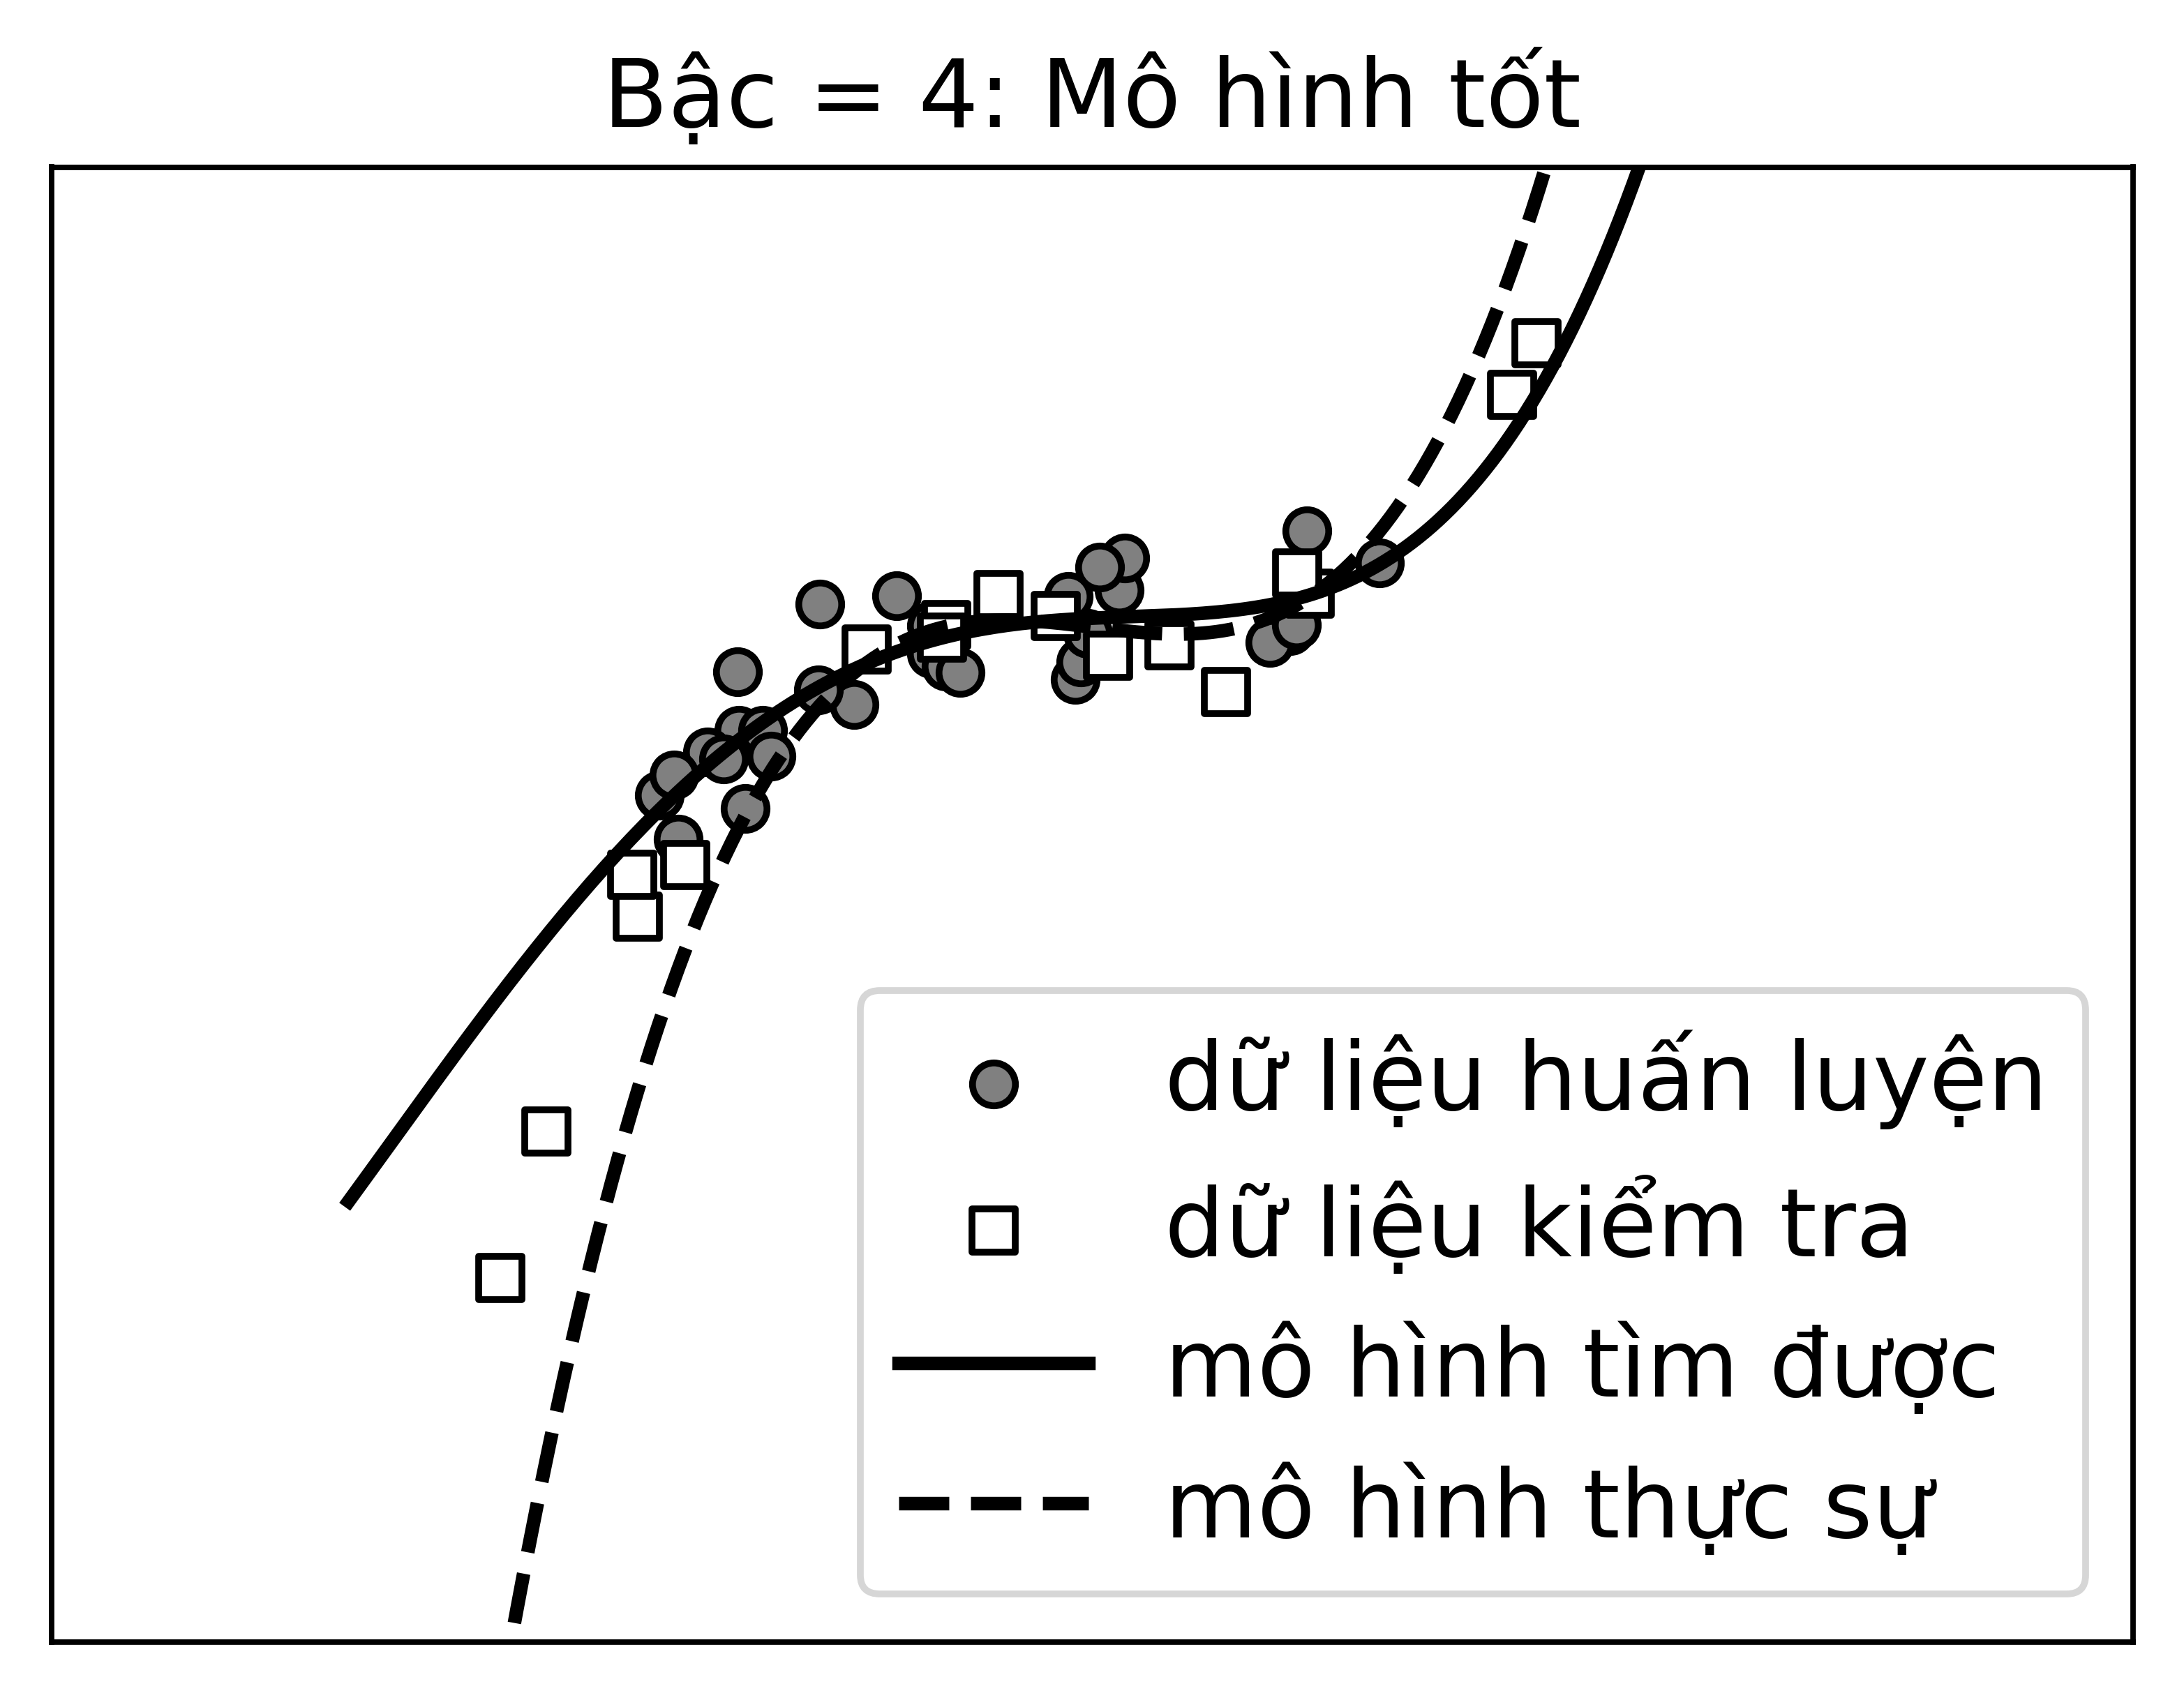
\includegraphics[width=0.99\linewidth]{ebookML_src/src/overfitting/poly4.png}
% {Chapters/01_Overview/15_overfitting/linreg_4.png}
\caption{}
\label{fig:15_polyregb}
\end{subfigure}
\begin{subfigure}{0.49\textwidth}
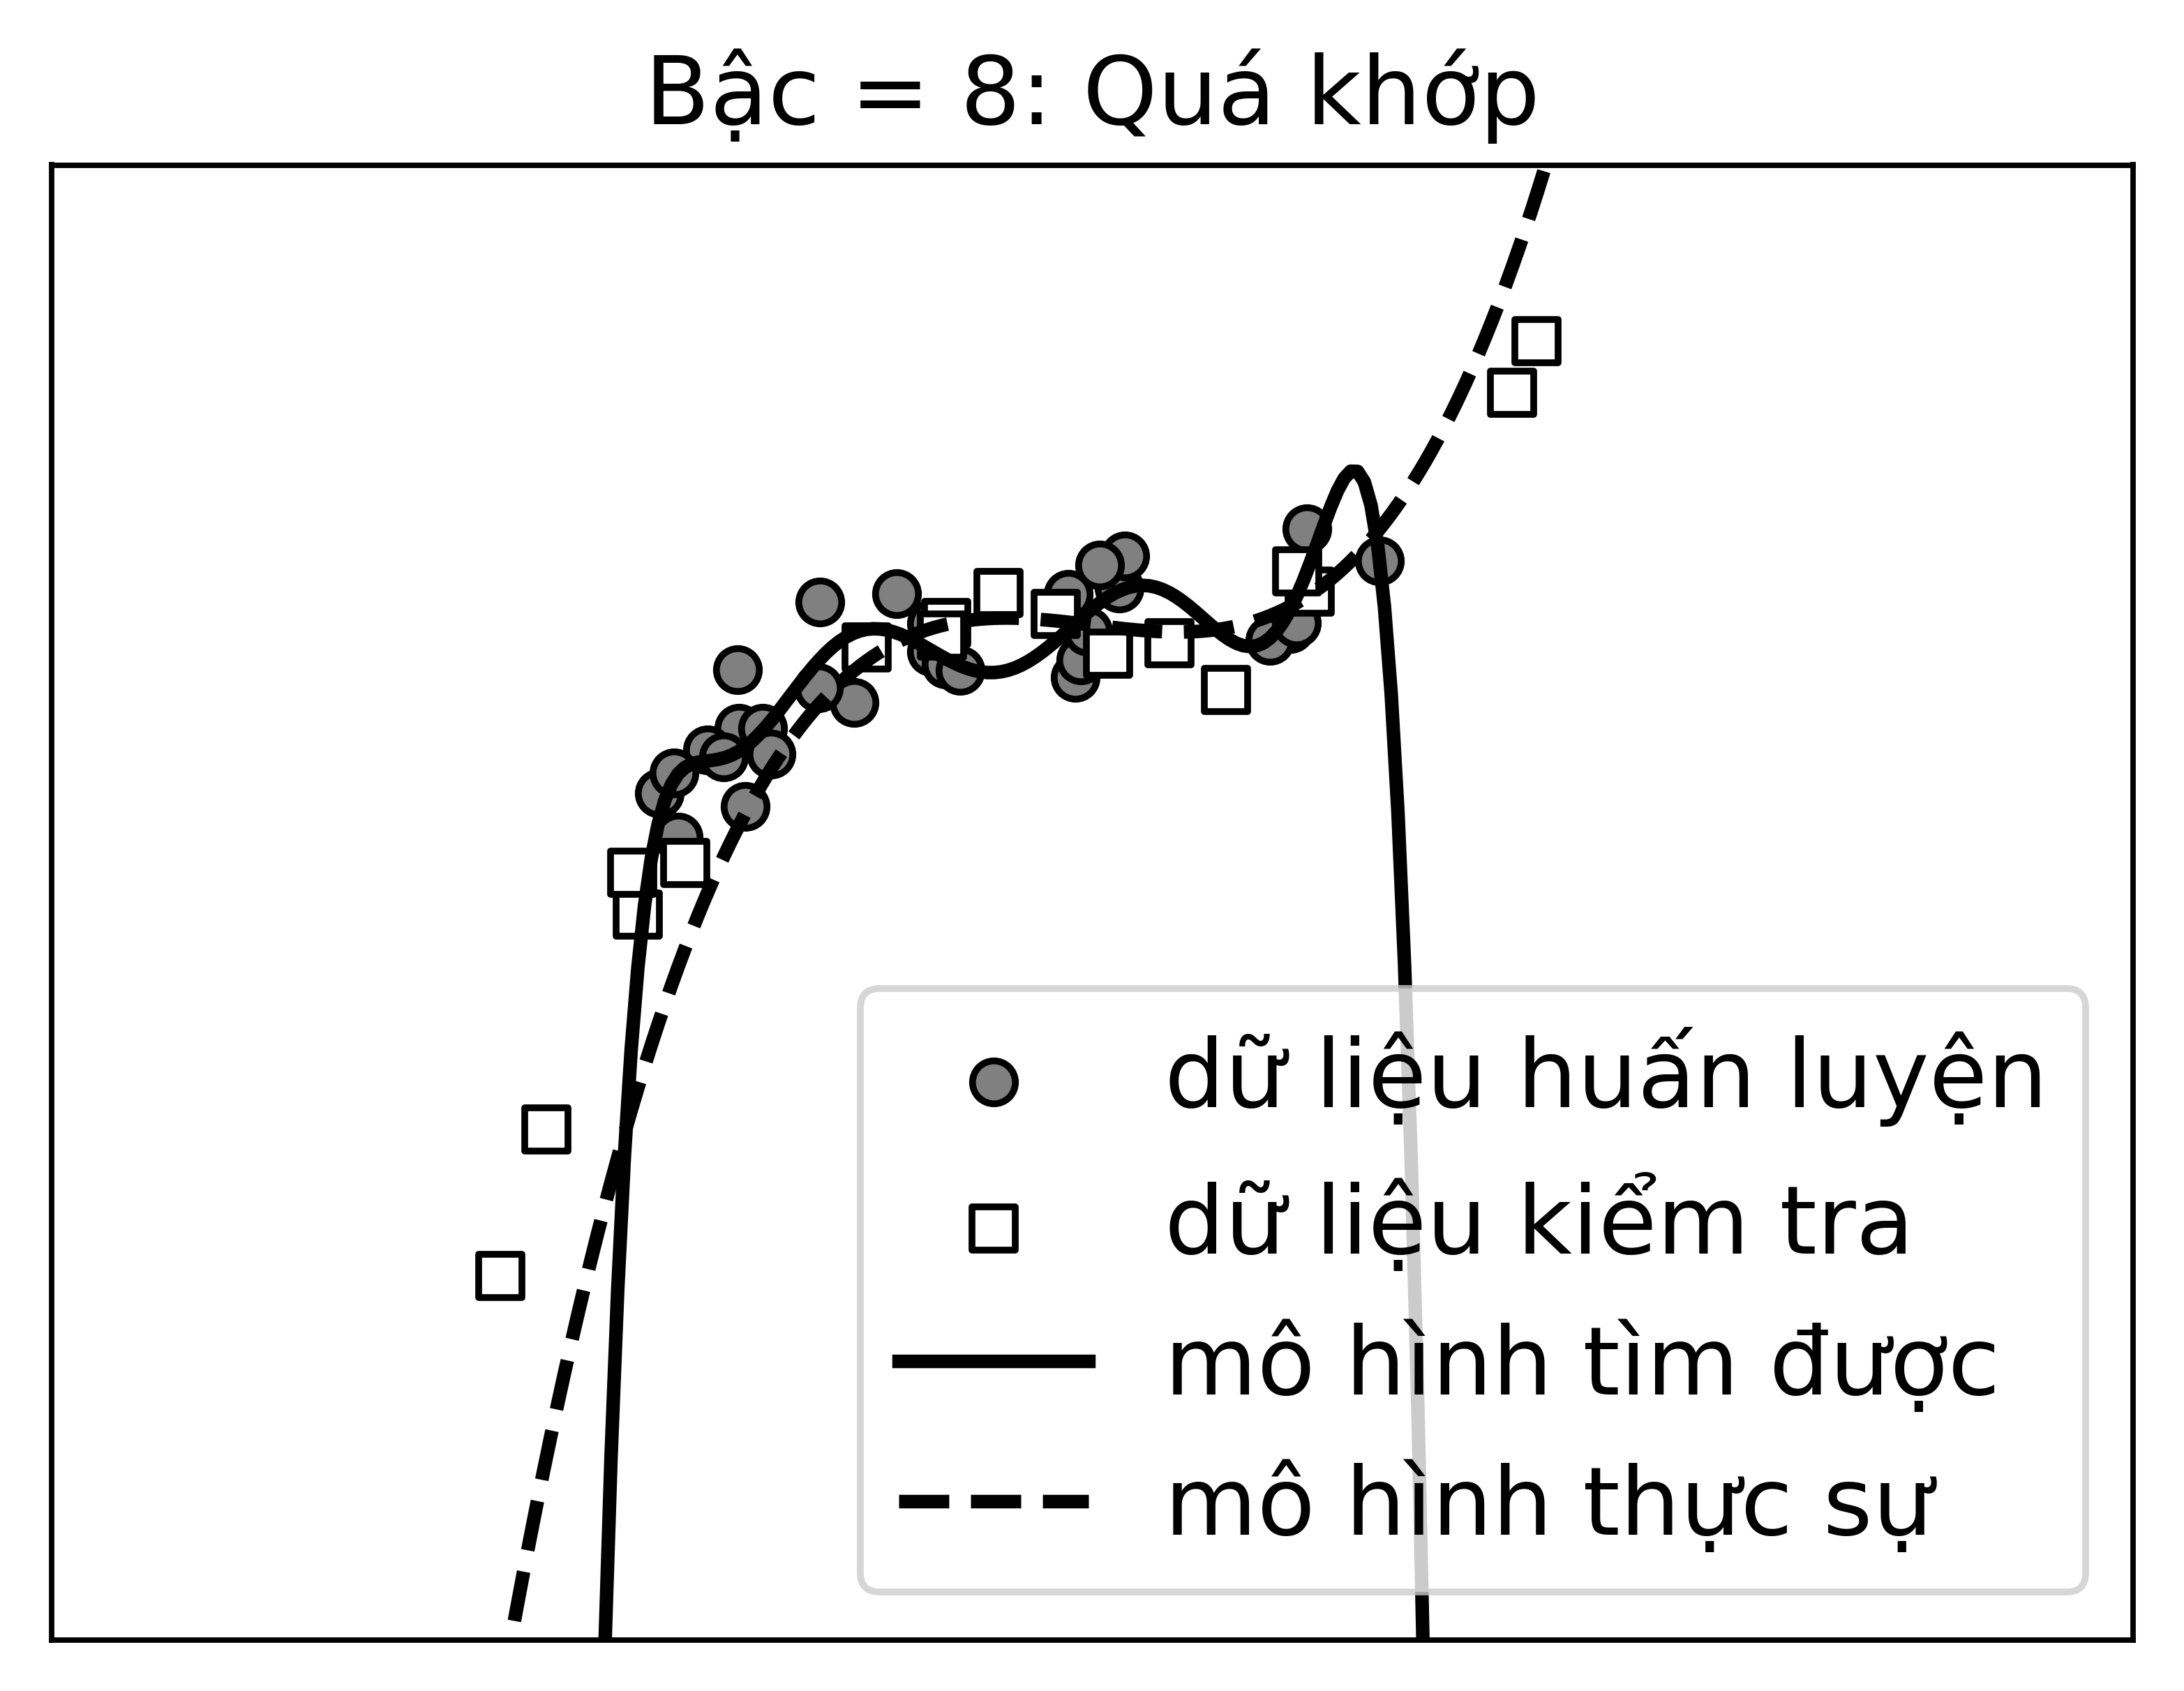
\includegraphics[width=0.99\linewidth]{ebookML_src/src/overfitting/poly8.png}
% {Chapters/01_Overview/15_overfitting/linreg_8.png}
\caption{}
\label{fig:15_polyregc}
\end{subfigure}
\begin{subfigure}{0.49\textwidth}
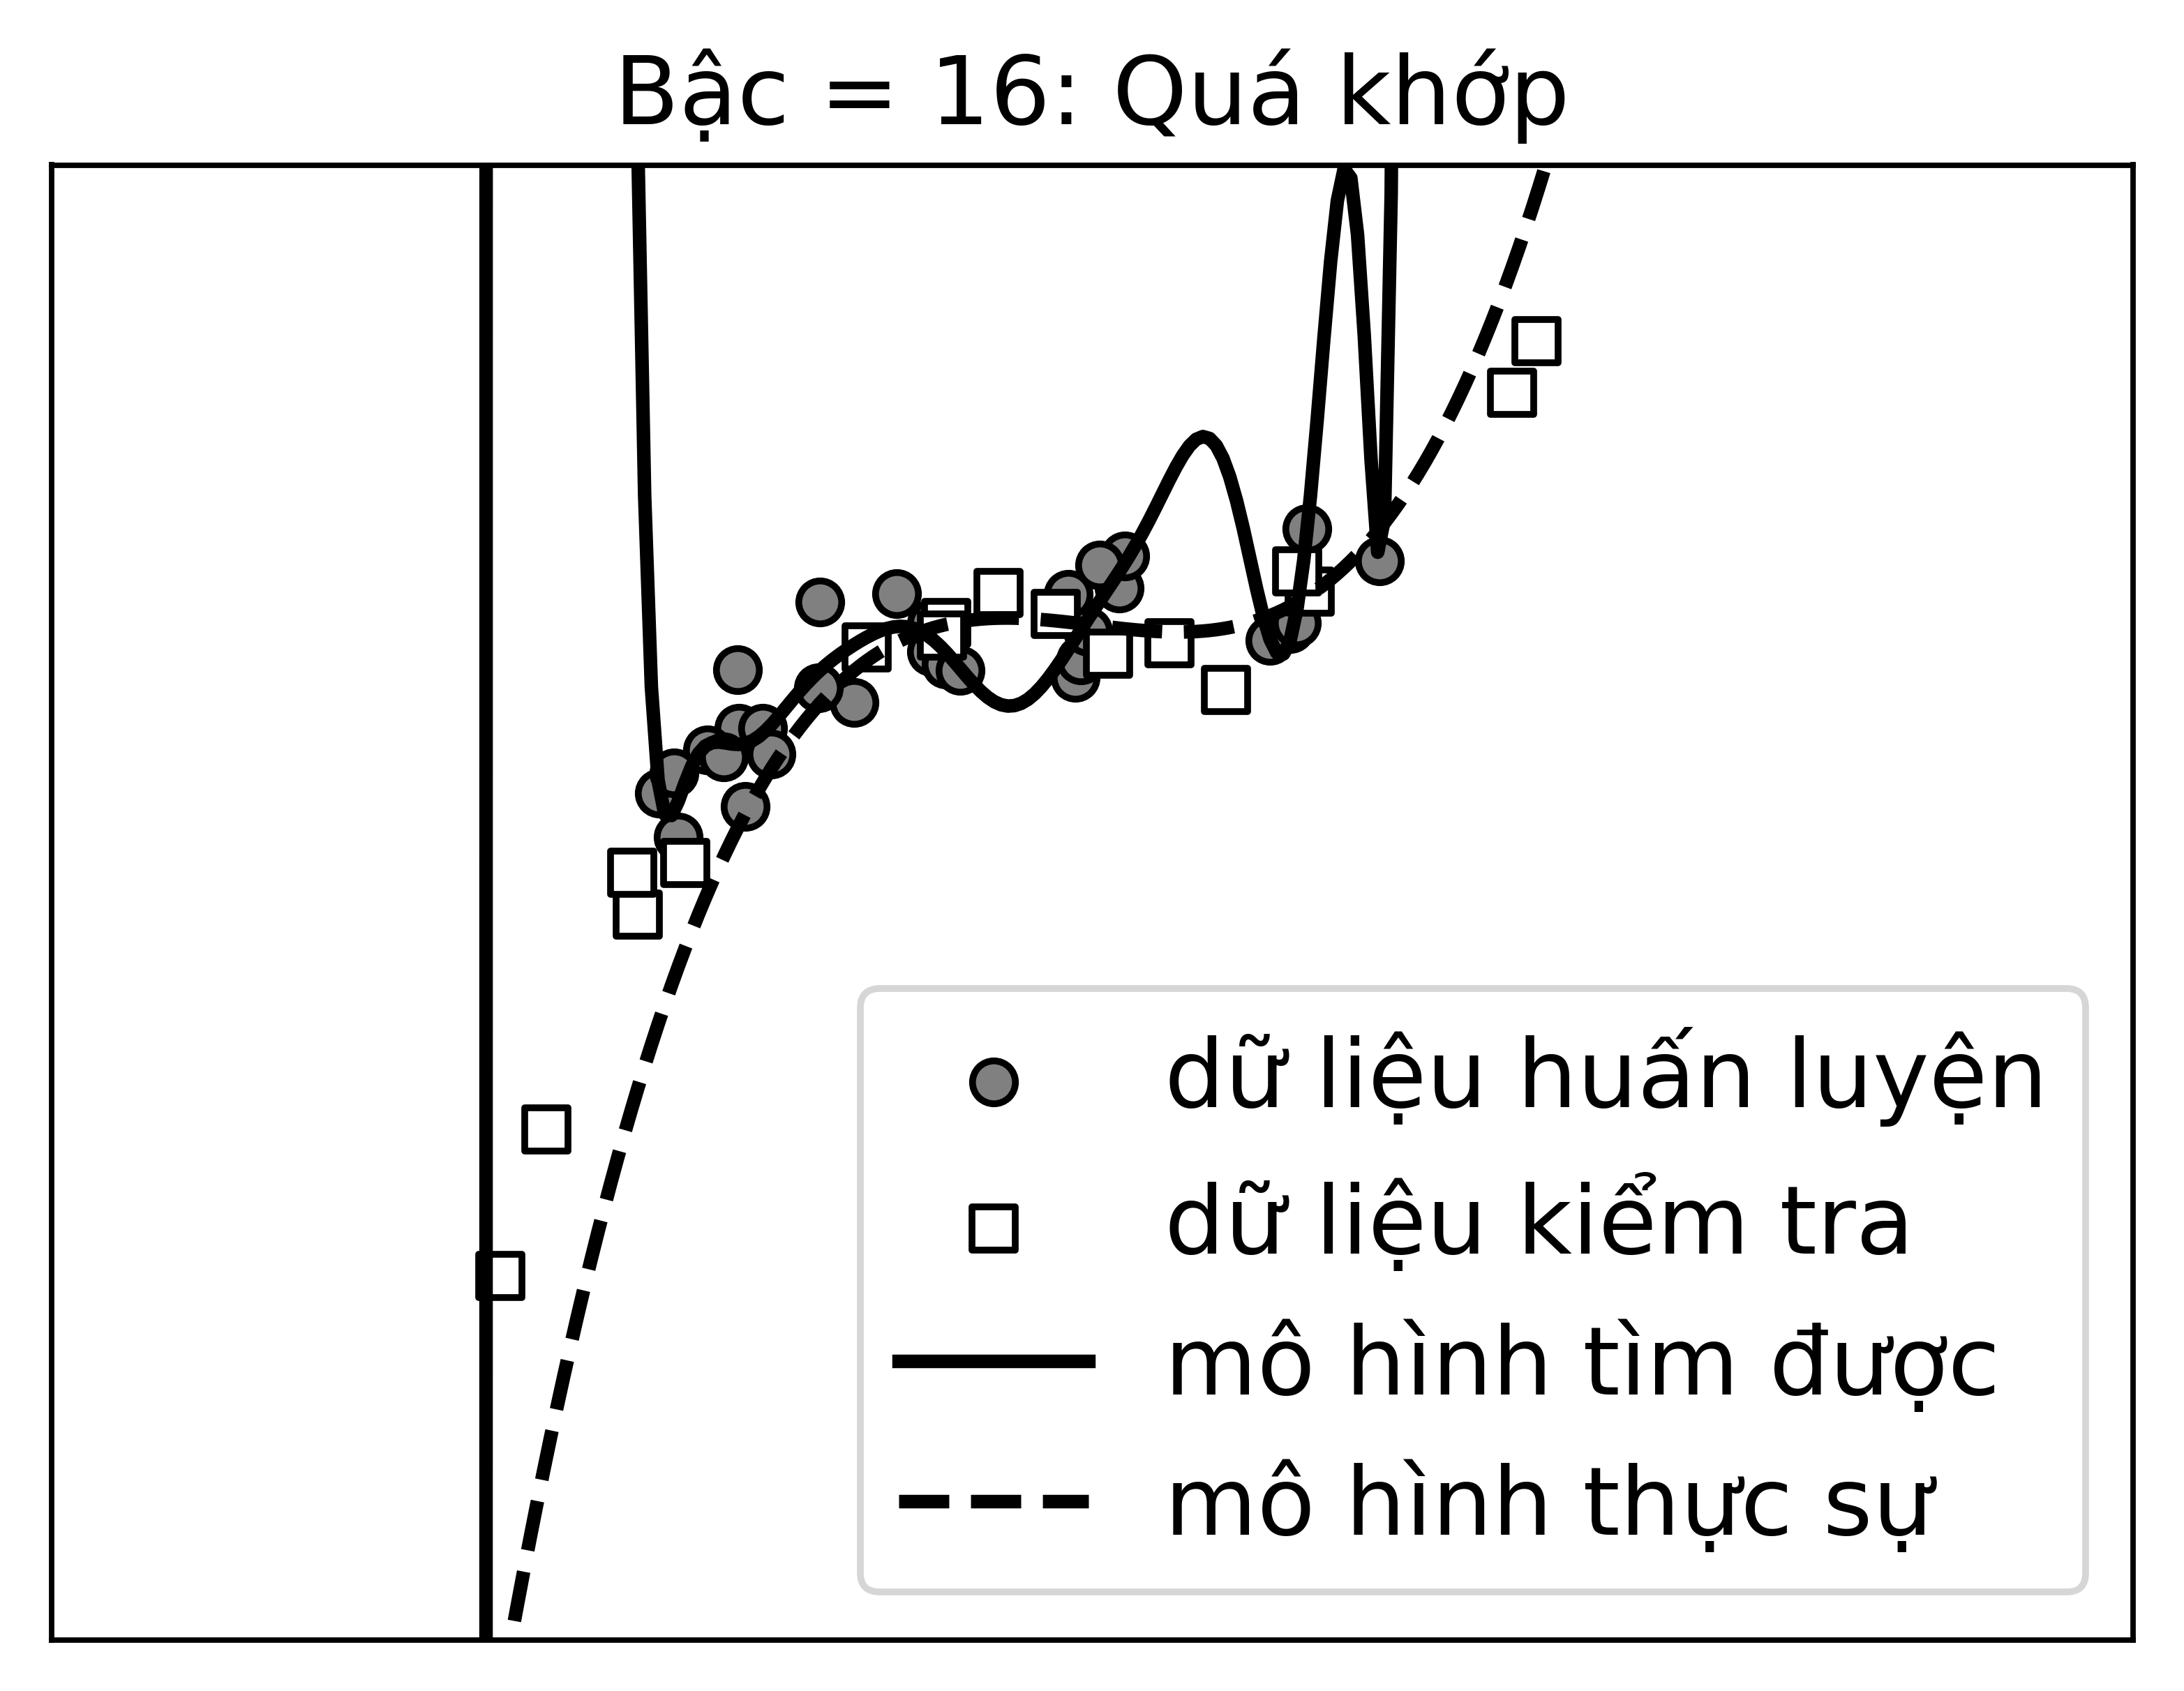
\includegraphics[width=0.99\linewidth]{ebookML_src/src/overfitting/poly16.png}
% {Chapters/01_Overview/15_overfitting/linreg_16.png}
\caption{}
\label{fig:15_polyregd}
\end{subfigure}
\caption{
Chưa khớp và quá khớp trong hồi quy đa thức.
}
\label{fig:15_polyreg}
\end{figure}

Như đã đề cập trong Chương~\ref{cha:linear_regression}, với loại dữ liệu này,
chúng ta có thể áp dụng hồi quy đa thức với vector đặc trưng
$\mathbf{x} = [1, x, x^2, x^3, \dots, x^d]^T$ cho đa thức bậc $d$. Điều quan
trọng là cần xác định bậc $d$ của đa thức. Giá trị $d$ còn được gọi là siêu tham số của mô hình.

\index{hồi quy đa thức -- polynomial regression}
\index{polynomial regression -- hồi quy đa thức}
\index{chưa khớp -- underfitting}
\index{underfitting -- chưa khớp}
Rõ ràng một đa thức bậc không vượt quá 29 có thể mô tả chính xác dữ liệu huấn
luyện. Tuy nhiên, ta sẽ xem xét các đa thức bậc thấp hơn $d = 2, 4, 8, 16$. Với
$d = 2$, mô hình không thực sự tốt vì mô hình dự đoán (đường nét liền) quá khác
so với {mô hình thực}; thậm chí nó có xu hướng đi xuống khi dữ liệu đang
có hướng đi lên. Trong trường hợp này, ta nói mô hình bị \textit{chưa khớp} (underfitting).
Khi $d = 8$, với các điểm dữ liệu trong tập huấn luyện, mô hình dự đoán và mô
hình thực khá giống nhau. Tuy nhiên, đa thức bậc 8 cho kết quả hoàn toàn ngược
với {xu hướng của dữ liệu} ở phía phải. Điều tương tự xảy ra trong trường hợp $d
= 16$. Đa thức bậc 16 này quá khớp với tập huấn luyện. Việc quá khớp
trong trường hợp bậc 16 là không tốt vì mô hình có thể đang cố gắng mô tả
{nhiễu} thay vì dữ liệu. Hiện tượng xảy ra ở hai trường hợp đa thức bậc
cao này chính là quá khớp. Độ phức tạp của đồ thị trong hai
trường hợp này cũng khá lớn, dẫn đến các đường dự đoán không được tự nhiên. Khi bậc của đa thức tăng lên, độ phức tạp của nó cũng tăng theo và hiện tượng quá khớp xảy ra nghiêm trọng hơn.

% \textit{Nếu bạn nào biết về Đa thức nội suy Lagrange thì có thể hiểu được hiện tượng sai số lớn với các điểm nằm ngoài khoảng của các điểm đã cho. Đó chính là lý do phương pháp đó có từ "nội suy", với các trường hợp "ngoại suy", kết quả thường không chính xác.}

Với $d = 4$, mô hình dự đoán khá giống với mô hình thực. Hệ số bậc cao nhất tìm
được rất gần với không\footnote{Mã nguồn tại \url{https://goo.gl/uD9hm1}.}, vì
vậy đa thức bậc bốn này khá gần với đa thức bậc ba ban đầu. Đây chính là một mô
hình tốt.


Quá khớp sẽ gây ra hậu quả lớn nếu trong tập huấn luyện có nhiễu. Khi
đó, mô hình quá chú trọng vào việc bắt chước tập huấn luyện mà quên đi việc
quan trọng hơn là tính tổng quát. Quá khớp đặc biệt xảy ra khi lượng dữ liệu huấn
luyện quá nhỏ hoặc độ phức tạp của mô hình quá cao. Trong ví dụ trên đây, độ
phức tạp của mô hình có thể được coi là bậc của đa thức cần tìm.

% Trong
% \href{http://machinelearningcoban.com/2017/02/24/mlp/}{Multi-layer Perceptron},
% độ phức tạp của mô hình có thể được coi là số lượng hidden layers và số lượng
% units trong các hidden layers.

Vậy, có những kỹ thuật nào giúp tránh quá khớp?

Trước hết, chúng ta cần một vài đại lượng để đánh giá chất lượng của mô hình
trên tập huấn luyện và tập kiểm tra. Dưới đây là hai đại lượng đơn giản, với
giả sử $\mathbf{y}$ là đầu ra thực sự, và $\mathbf{\hat{y}}$ là đầu ra dự đoán
của mô hình. Ở đây, đầu ra có thể là một vector.

\index{sai số huấn luyện}
\index{sai số trung bình bình phương -- mean squared error, MSE}
\index{mean squared error, MSE -- sai số trung bình bình phương}
\textbf{Sai số huấn luyện} (training error): Đại lượng này là mức độ sai khác giữa đầu ra thực và đầu
ra dự đoán của mô hình. Trong nhiều trường hợp, giá trị này chính là hàm mất mát khi áp dụng lên dữ liệu huấn luyện. Hàm mất mát này cần có một thừa số $\displaystyle
\frac{1}{N_{\text{train}}}$ để tính giá trị trung bình mất mát
trên mỗi điểm dữ liệu. Với các bài toán hồi quy, đại lượng này thường được xác định bởi \textit{sai số trung bình bình phương} ({mean squared error -- MSE}):
\begin{equation*}
\text{sai số huấn luyện}= \frac{1}{2N_{\text{train}}} \sum_{\text{tập huấn luyện}}
\|\mathbf{y} - \mathbf{\hat{y}}\|_2^2
\end{equation*}
% với $p$ \href{http://machinelearningcoban.com/math/#mot-so-chuan-thuong-dung}{thường bằng 1 hoặc 2}.
Với các bài toán phân loại, có nhiều cách đánh giá mô hình trên các tập dữ liệu. Chúng ta sẽ dần thấy trong các chương sau.

\textbf{Sai số kiểm tra} (test error): Tương tự như trên, áp dụng mô hình tìm được vào dữ liệu kiểm tra. Chú ý rằng dữ liệu kiểm tra không được sử dụng khi xây dựng mô hình. Với các mô hình hồi quy, đại lượng này thường được định nghĩa bởi
\begin{equation*}
\text{sai số kiểm tra}= \frac{1}{2N_{\text{test}}} \sum_{\text{tập kiểm tra}} \|\mathbf{y} - \mathbf{\hat{y}}\|_2^2
\end{equation*}
{Việc lấy trung bình là quan trọng vì lượng dữ liệu trong tập huấn
luyện và tập kiểm tra có thể chênh lệch nhau.}

Một mô hình được coi là tốt nếu cả {sai số huấn luyện} và {test
error} đều thấp. Nếu {sai số huấn luyện} thấp nhưng {sai số kiểm tra} cao,
ta nói mô hình bị quá khớp. Nếu {sai số huấn luyện} cao và {sai số kiểm tra} cao, ta nói mô hình bị chưa khớp. Xác suất để xảy ra việc
{sai số huấn luyện} cao nhưng {sai số kiểm tra} thấp là rất nhỏ.
%  .
% Chúng ta cùng đi vào phương pháp đầu tiên
Trong chương này, chúng ta sẽ làm quen với hai kỹ thuật phổ biến giúp tránh
quá khớp là \textit{xác thực} và \textit{cơ chế kiểm soát}.

\section{Xác thực}
\index{validation -- xác thực}
\index{xác thực -- validation}
\subsection{Xác thực}
% Chúng ta đã quen với việc chia tập dữ liệu ra thành hai tập nhỏ: training data
% và dữ liệu kiểm tra. Và một điều tôi vẫn muốn nhắc lại là khi xây dựng mô hình, ta không được sử dụng dữ liệu kiểm tra. Vậy làm cách nào để biết được chất lượng của mô hình với \textit{unseen data} (tức dữ liệu chưa nhìn thấy bao giờ)?

Một mô hình được coi là tốt nếu cả sai số huấn luyện và sai số kiểm tra đều nhỏ. Tuy
nhiên, nếu xây dựng một mô hình {chỉ} dựa trên tập huấn luyện, làm thế nào để
biết được chất lượng của nó trên tập kiểm tra?
\index{tập xác thực -- validation set}
\index{validation set -- tập xác thực}
Phương pháp đơn giản nhất là {trích} từ tập huấn luyện ra một tập con nhỏ và
thực hiện việc đánh giá mô hình trên tập dữ liệu này. Tập dữ liệu này được gọi
là \textit{tập xác thực} ({validation set}). Lúc này, {tập huấn luyện mới
là phần còn lại của tập huấn luyện ban đầu}.

Việc này khá giống với việc chúng ta ôn thi. Giả sử đề thi của các năm trước là
tập huấn luyện, đề thi năm nay là tập kiểm tra mà ta chưa biết. Khi chuẩn bị,
ta thường chia đề các năm trước ra hai phần: phần thứ nhất có thể xem lời giải
và tài liệu để ôn tập, phần còn lại được sử dụng để tự đánh giá kiến thức sau
khi ôn tập. Lúc này, phần thứ nhất đóng vai trò là tập huấn luyện mới, trong khi
phần thứ hai chính là tập xác thực. Nếu kết quả bài làm trên phần thứ hai là
khả quan, ta có thể tự tin hơn khi vào bài thi thật.




Lúc này, ngoài sai số huấn luyện và sai số kiểm tra, có thêm một đại lượng nữa ta cần
quan tâm là \textit{sai số xác thực} (validation error) được định nghĩa tương tự trên tập xác thực.
Với khái niệm mới này, ta tìm mô hình sao cho cả {sai số huấn luyện} và {sai số xác thực}
đều nhỏ, qua đó có thể dự đoán được rằng {sai số kiểm tra} cũng nhỏ. Để làm điều
đó, ta có thể huấn luyện nhiều mô hình khác nhau dựa trên tập huấn luyện, sau đó
áp dụng các mô hình tìm được và tính {sai số xác thực}. Mô hình cho {sai số xác thực}
nhỏ nhất sẽ là một mô hình tốt.

Thông thường, ta bắt đầu từ mô hình đơn giản, sau đó tăng dần độ phức tạp của mô
hình. Khi độ phức tạp tăng lên, sai số huấn luyện sẽ có xu hướng nhỏ dần, nhưng
điều tương tự có thể không xảy ra ở sai số xác thực. Lỗi xác thực ban đầu
thường giảm dần và đến một lúc sẽ tăng lên do quá khớp xảy ra khi độ phức tạp của mô hình tăng lên. Để chọn ra một mô hình tốt, ta quan
sát sai số xác thực. Khi {sai số xác thực} có chiều hướng tăng lên, ta chọn mô hình tốt nhất trước đó.



% <div class="imgcap">
% <img src ="\assets\15_overfitting\linreg_val.png" align = "center" width = "500">
% <div class = "thecap">Hình 2: Lựa chọn mô hình dựa trên validation (<a href = "https://github.com/tiepvupsu/tiepvupsu.github.io/blob/master/assets/15_overfitting/LinReg-validation.ipynb">Source code</a>).</div>
% </div>

\begin{figure}[t]
% caption on side
\floatbox[{\capbeside\thisfloatsetup{capbesideposition={right,top},capbesidewidth=6cm}}]{figure}[\FBwidth]
{\caption{
Lựa chọn mô hình dựa trên sai số xác thực
}
\label{fig:15_validerror}}
{ % figure here
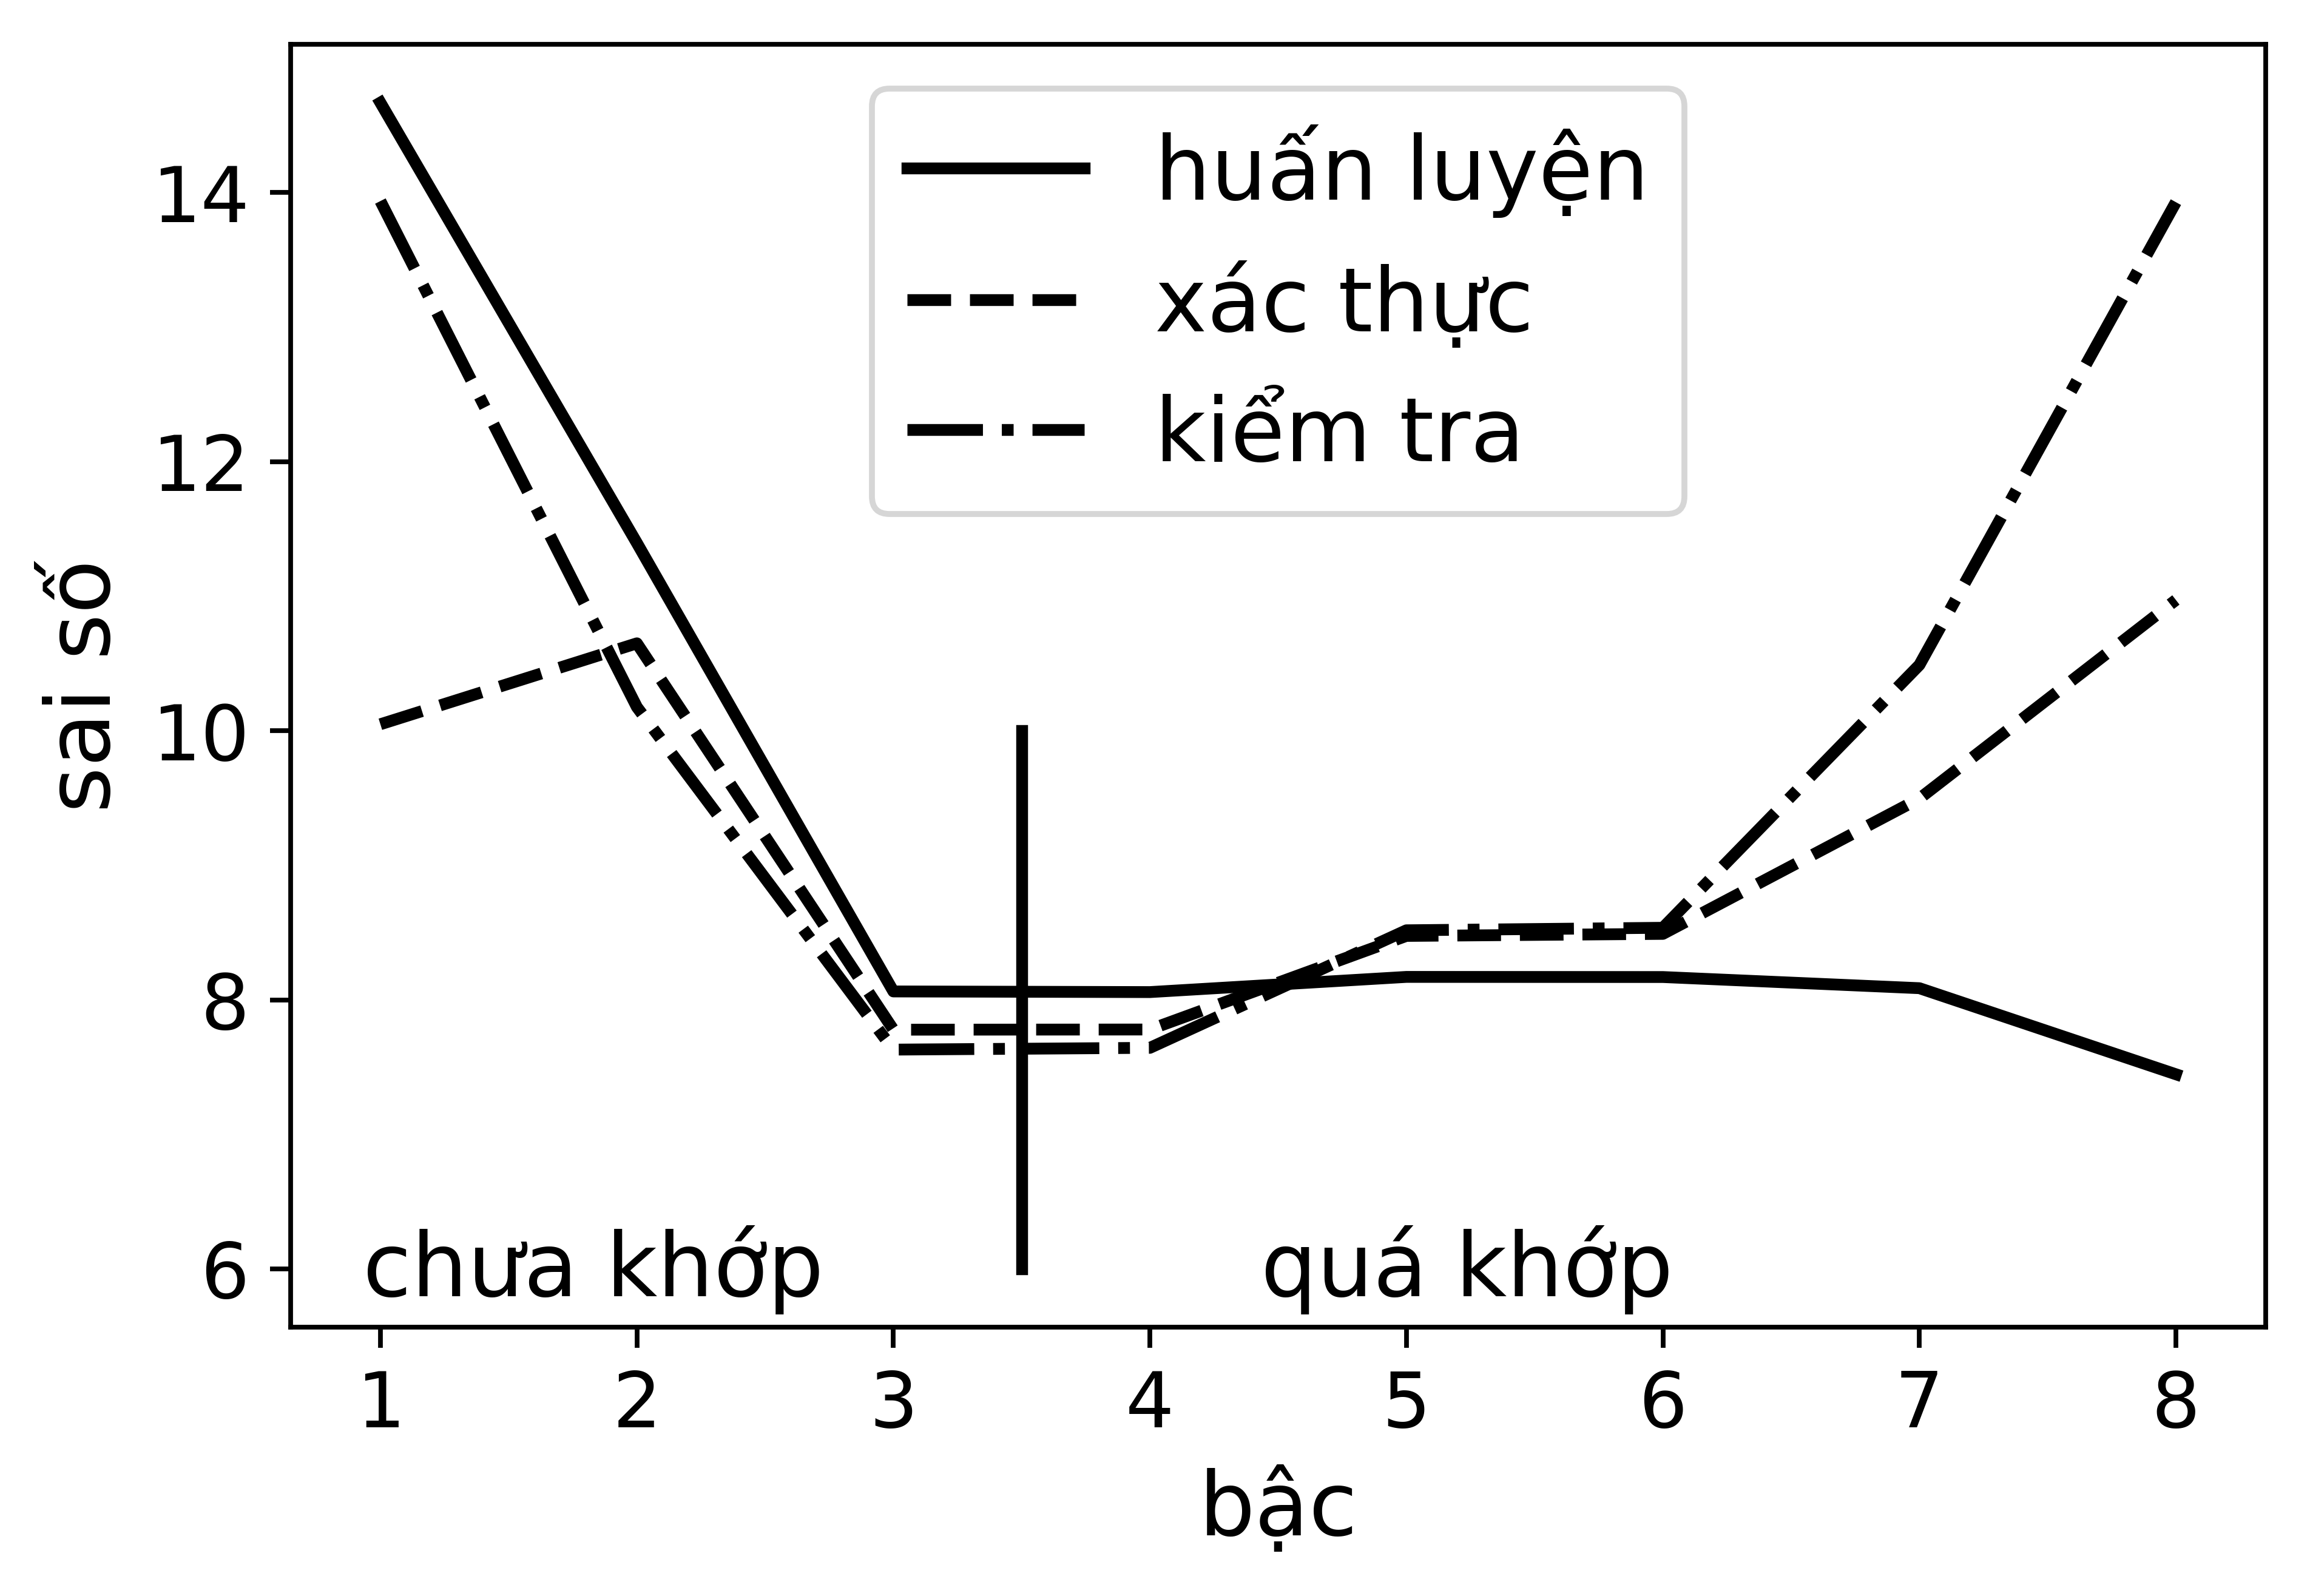
\includegraphics[width=.5\textwidth]{Chapters/01_Overview/15_overfitting/linreg_val.png}
}
\end{figure}
\index{tham số mô hình -- model parameter}
\index{model parameter -- tham số mô hình}
\index{siêu tham số mô hình -- model hyperparameter}
\index{model hyperparameter -- siêu tham số mô hình}
Hình~\ref{fig:15_validerror} mô tả ví dụ ở đầu chương với bậc của đa thức tăng
từ một đến tám. Tập xác thực là 10 điểm được lấy ra ngẫu nhiên từ tập huấn luyện
30 điểm ban đầu. Chúng ta hãy tạm chỉ xét hai đường nét liền và nét đứt, tương
ứng với {sai số huấn luyện} và {sai số xác thực}. Khi bậc của đa thức tăng lên,
{sai số huấn luyện} có xu hướng giảm. Điều này dễ hiểu vì đa thức bậc càng cao,
việc xấp xỉ càng chính xác. Quan sát đường nét đứt, khi bậc của đa thức là ba
hoặc bốn thì {sai số xác thực} thấp, sau đó nó tăng dần lên. Dựa vào
{sai số xác thực}, ta có thể xác định được bậc cần chọn là ba hoặc bốn. Quan
sát tiếp đường nét chấm gạch, tương ứng với {sai số kiểm tra}. Thật trùng hợp, sai số kiểm tra cũng đạt giá trị nhỏ nhất tại bậc bằng ba hoặc bốn và tăng lên khi bậc
tăng lên. Ở đây, kỹ thuật này đã tỏ ra hiệu quả. Mô hình phù hợp là mô hình có
bậc bằng ba hoặc bốn. Trong ví dụ này, tập xác thực đóng vai trò tìm ra bậc
của đa thức, tập huấn luyện đóng vai trò tìm các hệ số của đa thức
với bậc đã biết. Các hệ số của đa thức chính là các tham số mô hình,
trong khi bậc của đa thức có thể được coi là {siêu tham số}. Cả tập
huấn luyện và tập xác thực đều đóng vai trò xây dựng mô hình. Nhắc lại rằng
hai tập hợp này được tách ra từ tập huấn luyện ban đầu.

Trong ví dụ trên, ta vẫn thu được kết quả khả quan trên tập kiểm tra mặc dù không sử dụng tập này trong việc huấn luyện. Việc này xảy ra vì ta đã giả sử rằng dữ liệu xác thực và dữ liệu kiểm tra
có chung một đặc điểm nào đó (chung phân phối và đều chưa được mô hình nhìn thấy
khi huấn luyện).

Để ý rằng, khi bậc nhỏ bằng một hoặc hai, cả ba sai số đều cao, khi đó chưa khớp xảy ra.



\subsection{Xác thực chéo}
\label{ssec:crosvalid}
\index{xác thực -- validation!xác thực chéo -- cross-validation}
\index{validation -- xác thực!cross-validation -- xác thực chéo}
\index{xác thực -- validation!xác thực chéo k-fold}
\index{validation -- xác thực!xác thực chéo k-fold}
\index{xác thực -- validation!leave-one-out}
\index{validation -- xác thực!leave-one-out}

Trong nhiều trường hợp, lượng dữ liệu để xây dựng mô hình là hạn chế. Nếu lấy
quá nhiều dữ liệu huấn luyện ra làm dữ liệu xác thực, phần dữ liệu còn lại không
đủ để xây dựng mô hình. Lúc này, tập xác thực phải thật nhỏ để giữ được lượng dữ
liệu huấn luyện đủ lớn. Tuy nhiên, một vấn đề khác nảy sinh. Việc đánh giá trên tập xác thực quá nhỏ có thể gây ra hiện tượng thiên lệch. Có giải pháp nào cho tình huống này không?

Câu trả lời là \textit{xác thực chéo} ({cross-validation}).

Trong xác thực chéo, tập huấn luyện được chia thành $k$ tập con có kích thước gần bằng nhau và không giao nhau. Tại mỗi lần thử, một trong $k$ tập con đó được lấy ra làm tập xác thực, $k-1$ tập con còn lại được coi là tập huấn luyện. Như vậy, với mỗi bộ tham số mô hình, ta có $k$ mô hình khác nhau. Sai số huấn luyện và sai số xác thực được tính là trung bình cộng của các giá trị tương ứng trong $k$ mô hình đó. Cách làm này có tên gọi là \textit{xác thực chéo k-fold} (k-fold cross validation).

Khi $k$ bằng với số lượng phần tử trong tập huấn luyện ban đầu, tức mỗi
tập con có đúng một phần tử, ta gọi kỹ thuật này là \textit{leave-one-out}.

Thư viện scikit-learn hỗ trợ rất nhiều phương pháp phân chia dữ liệu để xây dựng mô hình. Bạn đọc có thể xem thêm
\textit{Cross-validation: evaluating estimator performance} (\url{https://goo.gl/Ars2cr}).





\section{Cơ chế kiểm soát}

\index{cơ chế kiểm soát -- regularization}
\index{regularization -- cơ chế kiểm soát}
Một nhược điểm lớn của xác thực chéo là số lượng mô hình cần huấn luyện tỉ lệ
thuận với $k$. Điều đáng nói là mô hình hồi quy đa thức như trên chỉ có một siêu
tham số liên quan đến độ phức tạp của mô hình cần xác định là bậc của đa thức.
Trong nhiều bài toán, lượng siêu tham số cần xác định thường lớn hơn, và
khoảng giá trị của mỗi tham số cũng rộng hơn, chưa kể có những
tham số có thể là số thực. Điều này dẫn đến việc huấn luyện nhiều mô hình là khó
khả thi. Có một kỹ thuật tránh quá khớp khác giúp giảm số mô hình cần huấn
luyện có tên là \textit{cơ chế kiểm soát} (regularization).

{Cơ chế kiểm soát} là một kỹ thuật phổ biến giúp tránh quá khớp theo hướng làm
giảm độ phức tạp của mô hình. Việc giảm độ phức tạp này có thể khiến lỗi huấn
luyện tăng lên nhưng lại làm tăng tính tổng quát của mô hình. Dưới đây là một
vài kỹ thuật kiểm soát.

\subsection{Kết thúc sớm}
\index{kết thúc sớm -- early stopping}
\index{early stopping -- kết thúc sớm}
Các mô hình machine learning phần lớn được xây dựng thông qua lặp đi lặp lại một
quy trình tới khi hàm mất mát hội tụ. Nhìn chung, giá trị hàm mất mát giảm dần
khi số vòng lặp tăng lên. Một giải pháp giúp giảm quá khớp là dừng thuật toán
trước khi nó hội tụ. Giải pháp này có tên là \textit{kết thúc sớm} (early stopping).

Vậy kết thúc khi nào là phù hợp? Kỹ thuật thường dùng là tách từ tập huấn luyện ra
một tập xác thực. Khi huấn luyện, ta tính toán cả sai số huấn luyện và sai số
xác thực, nếu sai số huấn luyện vẫn có xu hướng giảm nhưng sai số xác thực có xu
hướng tăng lên thì ta kết thúc thuật toán.

%  Sau một vòng lặp, ta tính cả \textit{sai số huấn luyện} và \textit{sai số xác thực}, đến khi \textit{sai số xác thực} có chiều hướng tăng lên thì dừng lại, và quay lại sử dụng mô hình tương ứng với điểm và \textit{sai số xác thực} đạt giá trị nhỏ.

% <div class="imgcap">
% <img src ="\assets\15_overfitting\EarlyStopping.png" align = "center" width = "400">
% <div class = "thecap">Hình 3: Early Stopping. Đường màu xanh là <i>sai số huấn luyện</i>, đường màu đỏ là <i>sai số xác thực</i>. Trục x là số lượng vòng lặp, trục y là error. Mô hình được xác định tại vòng lặp mà <i>sai số xác thực</i> đạt giá trị nhỏ nhất.  (<a href = "https://en.wikipedia.org/wiki/Overfitting">Overfitting - Wikipedia</a>).</div>
% </div>

\begin{figure}[t]
% caption on side
\floatbox[{\capbeside\thisfloatsetup{capbesideposition={right,top},capbesidewidth=6cm}}]{figure}[\FBwidth]
{\caption{
Kết thúc sớm. Thuật toán
huấn luyện dừng lại tại vòng lặp mà sai số xác thực đạt giá trị nhỏ nhất. }
\label{fig:15_earlystopping}}
{ % figure here

\includegraphics[width=.5\textwidth]{Chapters/01_Overview/15_overfitting/earlystopping_1.png}
}
\end{figure}


Hình~\ref{fig:15_earlystopping} mô tả cách tìm điểm \textit{kết thúc}. Chúng ta
thấy rằng phương pháp này tương tự phương pháp tìm bậc của đa thức ở đầu chương,
với độ phức tạp của mô hình có thể được coi là số vòng lặp cần chạy. Số vòng lặp
càng cao thì sai số huấn luyện càng nhỏ nhưng sai số xác thức có thể tăng lên, tức mô hình có khả năng bị quá khớp.


\subsection{Thêm số hạng vào hàm mất mát}
\index{tham số kiểm soát -- regularization parameter}
\index{regularization parameter -- tham số kiểm soát}
\index{hàm mất mát được kiểm soát -- regularized loss function}
\index{regularized loss function -- hàm mất mát được kiểm soát}
Kỹ thuật phổ biến hơn là thêm vào hàm mất mát một số hạng giúp
kiểm soát độ phức tạp mô hình. Số hạng này thường dùng để đánh giá độ phức tạp của
mô hình với giá trị lớn thể hiện mô hình phức tạp. {Hàm mất mát mới} được
gọi là \textit{hàm mất mát được kiểm soát} (regularized loss function), thường được định nghĩa như sau:
\begin{equation*}
\L_{\text{reg}}(\theta) = \L(\theta) + \lambda R(\theta)
\end{equation*}
Nhắc lại rằng $\theta$ được dùng để ký hiệu các tham số trong mô hình. $\L(\theta)$ là hàm mất mát phụ thuộc vào tập huấn luyện và $\theta$, $R(\theta)$ là số hạng kiểm soát chỉ phụ thuộc vào $\theta$. Số vô hướng $\lambda$ thường là một số dương nhỏ, còn được gọi là \textit{tham số kiểm soát} (regularization parameter).
Tham số kiểm soát thường được chọn là các giá trị nhỏ để đảm bảo nghiệm
của bài toán tối ưu $\L_{\text{reg}}(\theta)$ không quá xa nghiệm của bài toán
tối ưu $\L(\theta)$.

%  $\$
% Việc tối thiểu \textit{regularized loss function}, nói một cách tương đối, đồng nghĩa với việc tối thiểu cả \textit{loss function} và số hạng \textit{regularization}. Tôi dùng cụm "nói một cách tương đối" vì nghiệm của bài toán tối ưu \textit{loss function} và \textbf{regularized loss function} là khác nhau.  Chúng ta vẫn mong muốn rằng sự khác nhau này là nhỏ, vì vậy tham số regularization (\textit{regularizaton parameter}) $\lambda$ thường được chọn là một số nhỏ để biểu thức regularization không làm giảm quá nhiều chất lượng của nghiệm.

% Với các mô hình Neural Networks, một số kỹ thuật regularization thường được sử dụng là:

% Một vài hàm regularization thường được sử dụng được cho dưới đây:
\index{cơ chế kiểm soát -- regularization!kiểm soát $\ell_1$ -- $\ell_1$ regularization}
\index{regularization -- cơ chế kiểm soát!$\ell_1$ regularization -- kiểm soát $\ell_1$}
\index{cơ chế kiểm soát -- regularization!kiểm soát $\ell_2$ -- $\ell_2$ regularization}
\index{regularization -- cơ chế kiểm soát!$\ell_2$ regularization -- kiểm soát $\ell_2$}
\index{hồi quy ridge -- ridge regression}
\index{ridge regression -- hồi quy ridge}
\index{hồi quy lasso -- lasso regression}
\index{lasso regression -- hồi quy lasso}
\index{lựa chọn đặc trưng -- feature selection}
\index{feature selection -- lựa chọn đặc trưng}
% \index{sparsity}

Hai hàm kiểm soát phổ biến là $\ell_1$ norm và $\ell_2$ norm.
Ví dụ, khi chọn $R(\bw) = \|\bw\|_2^2$ cho hàm mất mát của hồi quy tuyến tính,
chúng ta sẽ thu được hồi quy ridge. Hàm kiểm soát $\ell_2$ này khiến các hệ số
trong $\bw$ không quá lớn, giúp tránh việc đầu ra phụ thuộc mạnh vào một
đặc trưng nào đó. Trong khi đó, nếu chọn $R(\bw) = \|\bw\|_1$, nghiệm $\bw$ tìm
được có xu hướng rất nhiều phần tử bằng không (\textit{nghiệm thưa}\footnote{\textit{L1 Norm Regularization and Sparsity Explained for
Dummies} (\url{https://goo.gl/VqPTLh}).}). Khi thêm kiểm soát $\ell_1$ vào
hàm mất mát của hồi quy tuyến tính, chúng ta thu được hồi quy LASSO. Các
thành phần khác không của $\bw$ tương đương với các đặc trưng quan trọng đóng
góp vào việc dự đoán đầu ra. Các đặc trưng ứng với thành phần bằng không của
$\bw$ được coi là ít quan trọng. Chính vì vậy, hồi quy LASSO cũng được coi là
một phương pháp giúp lựa chọn những đặc trưng hữu ích cho mô hình và có ý nghĩa trong việc trích chọn đặc trưng.

% \index{kháng nhiễu}
% \index{closed-form solution}
So với kiểm soát $\ell_2$, kiểm soát $\ell_1$ được cho là giúp mô hình kháng nhiễu tốt hơn. Tuy nhiên, hạn chế của kiểm soát $\ell_1$ là hàm $\ell_1$ norm không có đạo hàm mọi nơi, dẫn đến việc tìm nghiệm thường tốn thời gian hơn. Trong khi đó, đạo hàm của $\ell_2$ norm xác định mọi nơi. Hơn nữa, $\ell_2$ norm là một hàm lồi chặt, trong khi $\ell_1$ là một hàm lồi. Các tính chất của hàm lồi và hàm lồi chặt sẽ được thảo luận trong Phần~\ref{part:cvxopt}.


% \subsubsection{$l_2$ regularization}
% % Trong kỹ thuật này:
% \begin{equation*}
% R(\mathbf{w}) = \|\mathbf{w}\|_2^2
% \end{equation*}
% tức norm 2 của hệ số.
% \textit{Nếu bạn đọc chưa quen thuộc với khái niệm norm, bạn được khuyến khích đọc} \href{http://machinelearningcoban.com/math/#-norms-chuan}{phần phụ lục này}.

% Hàm số này có một vài đặc điểm đang lưu ý:

% \begin{itemize}
%     \item Thứ nhất, $\|\mathbf{w}\|_2^2$ là một hàm số \textit{rất mượt}, đạo hàm của nó đơn giản là $\mathbf{w}$, vì vậy đạo hàm của \textit{regularized loss function} cũng rất dễ tính, chúng ta có thể hoàn toàn dùng các phương pháp dựa trên gradient để cập nhật nghiệm. Cụ thể:
%     \begin{equation*}
%     \frac{\partial J_{\text{reg}} }{\partial \mathbf{w}} = \frac{\partial J}{\partial \mathbf{w}} + \lambda \mathbf{w}
%     \end{equation*}
%     \item Thứ hai, việc tối thiểu $\|\mathbf{w}\|_2^2$ đồng nghĩa với việc khiến cho các giá trị của hệ số $\mathbf{w}$ trở nên nhỏ gần với 0. Với Polynomial Regression, việc các hệ số này nhỏ có thể giúp các hệ số ứng với các số hạng bậc cao là nhỏ, giúp tránh overfitting. Với Multi-layer Pereceptron, việc các hệ số này nhỏ giúp cho nhiều hệ số trong các ma trận trọng số là nhỏ. Điều này tương ứng với việc số lượng các hidden units \textit{hoạt động} (khác không) là nhỏ, cũng giúp cho MLP tránh được hiện tượng overfitting.
% \end{itemize}

% $l_2$ regularization là kỹ thuật được sử dụng nhiều nhất để giúp Neural Networks tránh được overfitting. Nó còn có tên gọi khác là \textbf{weight decay}. \textit{Decay} có nghĩa là \textit{tiêu biến}.

% Trong Xác suất thống kê, Linear Regression với $l_2$ regularization được gọi là \href{https://en.wikipedia.org/wiki/Tikhonov_regularization}{\textbf{Ridge Regression}}. Hàm mất mát của \textit{Ridge Regression} có dạng:
% \begin{equation*}
% J(\mathbf{w}) = \frac{1}{2} \|\mathbf{y} - \mathbf{Xw}\|_2^2 + \lambda \|\mathbf{w}\|_2^2
% \end{equation*}
% trong đó, số hạng đầu tiên ở vế phải chính là hàm mất mát của Linear Regression. Số hạng thứ hai chính là phần regularization.


% \subsection{Tikhonov regularization}
% \begin{equation*}
% \lambda R(\mathbf{w}) = \|\Gamma \mathbf{w}\|_2^2
% \end{equation*}

% Với $\Gamma$ (viết hoa của gamma) là một ma trận. Ma trận $\Gamma$ hay được dùng nhất là ma trận đường chéo. Nhận thấy rằng $l_2$ regularization chính là một trường hợp đặc biệt của Tikhonov regularization với $\Gamma = \lambda \mathbf{I}$ với $\mathbf{I}$ là ma trận đơn vị (\textit{the identity matrix}), tức các phần tử trên đường chéo của $\Gamma$ là như nhau.

% Khi các phần tử trên đường chéo của $\Gamma$ là khác nhau, ta có một phiên bản gọi là \textit{weighted $l_2$ regularization}, tức đánh trọng số khác nhau cho mỗi phần tử trong $\mathbf{w}$. Phần tử nào càng bị đánh trọng số cao thì nghiệm tương ứng càng nhỏ (để đảm bảo rằng hàm mất mát là nhỏ). Với Polynomial Regression, các phần tử ứng với hệ số bậc cao sẽ được đánh trọng số cao hơn, khiến cho xác suất để chúng gần 0 là lớn hơn.


% \subsection{Regularizers for sparsity}

% Trong nhiều trường hợp, ta muốn các hệ số \textit{thực sự} bằng 0 chứ không phải là \textit{nhỏ gần 0} như $l_2$ regularization đã làm phía trên. Lúc đó, có một regularization khác được sử dụng, đó là $l_0$ regularization:
% \begin{equation*}
% R(\mathbf{W}) = \|\mathbf{w}\|_0
% \end{equation*}

% Norm 0 không phải là một norm thực sự mà là giả norm. (Bạn được khuyến khích đọc thêm về \href{http://machinelearningcoban.com/math/#-norms-chuan}{norms (chuẩn)}). Norm 0 của một vector là số các phần tử khác không của vector đó. Khi norm 0 nhỏ, tức rất nhiều phần tử trong vector đó bằng 0, ta nói vector đó là \textit{sparse}.

% Việc giải bài toán tổi thiểu norm 0 nhìn chung là khó vì hàm số này không \textit{convex}, không liên tục. Thay vào đó, norm 1 thường được sử dụng:
% \begin{equation*}
% R(\mathbf{W}) = \|\mathbf{w}\|_1 = \sum_{i=0}^d \|w_i\|
% \end{equation*}

% Norm 1 là tổng các trị tuyệt đối của tất cả các phần tử. Người ta đã chứng minh được rằng tối thiểu norm 1 sẽ dẫn tới nghiệm có nhiều phần tử bằng 0. Ngoài ra, vì norm 1 là một \textit{norm thực sự} (proper norm) nên hàm số này là \textit{convex}, và hiển nhiên là liên tục, việc giải bài toán này dễ hơn việc giải bài toán tổi thiểu norm 0. Về $l_1$ regularization, bạn đọc có thể đọc thêm trong \href{http://machinelearningcoban.com$l_1$ regularization}{lecture note} này. Việc giải bài toán $l_1$ regularization nằm ngoài mục đích của tôi trong bài viết này. Tôi hứa sẽ quay lại phần này sau. (Vì đây là phần chính trong nghiên cứu của tôi).

% Trong Thống Kê, việc sử dụng $l_1$ regularization còn được gọi là \href{https://en.wikipedia.org/wiki/Lasso_(statistics}{LASSO}) (Least Absolute Shrinkage and Selection Operator)).

% Khi cả $l_2$ và $l_1$ regularization được sử dụng, ta có mô hình gọi là \href{https://en.wikipedia.org/wiki/Elastic_net_regularization}{Elastic Net Regression}.


% \subsection{Regularization trong sklearn}

% Trong \href{http://scikit-learn.org/stable/modules/generated/sklearn.linear_model.LogisticRegression.html}{sklearn}, ví dụ \href{http://machinelearningcoban.com/2017/01/27/logisticregression/}{Logistic Regression}, bạn cũng có thể sử dụng các $l_1$ và $l_2$ regularizations bằng cách khai báo biến \pythoninline{penalty='l1'} hoặc \pythoninline{penalty = 'l2'} và biến \pythoninline{C}, trong đó \pythoninline{C} là \textit{nghịch đảo} của $\lambda$. Trong các bài trước khi chưa nói về  Overfitting và Regularization, tôi có sử dụng \pythoninline{C = 1e5} để chỉ ra rằng $\lambda$ là một số rất nhỏ.


% \section{Các phương pháp khác}
% Ngoài các phương pháp đã nêu ở trên, với mỗi mô hình, nhiều phương pháp tránh overfitting khác cũng được sử dụng. Điển hình là \href{http://jmlr.org/papers/volume15/srivastava14a/srivastava14a.pdf}{Dropout trong Deep Neural Networks mới được đề xuất gần đây}. Một cách ngắn gọn, dropout là một phương pháp \textit{tắt} ngẫu nhiên các units trong Networks. \textit{Tắt} tức cho các unit giá trị bằng không và tính toán feedforward và backpropagation bình thường trong khi training. Việc này không những giúp lượng tính toán giảm đi mà còn làm giảm việc overffitng. Tôi xin được quay lại vấn đề này nếu có dịp nói  sâu về Deep Learning trong tương lai.

% Bạn đọc có thể tìm đọc thêm với các từ khóa: \href{https://en.wikipedia.org/wiki/Pruning_(decision_trees}{pruning}) (tránh overftting trong Decision Trees), \href{https://en.wikipedia.org/wiki/VC_dimension}{VC dimension} (đo độ phức tạp của mô hình, độ phức tạp càng lớn thì càng dễ bị overfitting).


% \section{Tóm tắt và thảo luận}

% \subsection{bias variance tradeoff}

% \begin{itemize}
%     \item Một mô hình mô tốt là mộ mô hình có \textit{tính tổng quát}, tức mô tả
%     được dữ liệu cả trong lẫn ngoài tập huấn luyện. Mô hình chỉ mô tả tốt dữ
%     liệu trong tập huấn luyện được gọi là \textbf{overfitting}.

%     \item Để tránh overfitting, có rất nhiều kỹ thuật được sử dụng, điển hình là \textbf{cross-validation} và \textbf{regularization}. Trong Neural Networks, \textbf{weight decay} và \textbf{dropout} thường được dùng.
% \end{itemize}
\index{suy giảm trọng số -- weight decay}
\index{weight decay -- suy giảm trọng số}
Trong mạng neuron, phương pháp sử dụng kiểm soát $\ell_2$ còn được gọi là \textit{suy giảm trọng số} (weight decay)~\cite{krogh1992simple}. Ngoài ra, gần đây có một phương pháp kiểm soát rất hiệu quả cho các mạng neuron sâu được sử dụng là \textit{dropout}~\cite{srivastava2014dropout}.

\section{Đọc thêm}
\begin{enumerate}
\item A. Krogh \etal, \textit{A simple weight decay can improve generalization.} NIPS 1991~\cite{krogh1992simple}.

\item N. Srivastava \etal, \textit{Dropout: A Simple Way to Prevent Neural
Networks from  Overfitting}, Journal of Machine Learning Research 15.1
(2014): 1929-1958~\cite{srivastava2014dropout}.

\item \textit{Understanding the Bias-Variance Tradeoff} (\url{https://goo.gl/yvQv3w}).

\end{enumerate}


\setcounter{part}{2}
\setcounter{chapter}{8}
%!TEX root = ../book_ML.tex
\part{Khởi động}
\label{part:warmup}
Trong phần này, chúng ta sẽ làm quen với ba thuật toán machine learning chưa cần
nhiều tới tối ưu: $K$-lân cận cho các bài toán hồi quy và phân loại, $K$-means cho bài toán phân cụm và bộ phân loại naive Bayes cho dữ liệu dạng văn bản.

%!TEX root = ../../book_ML.tex
\chapter{$K$ lân cận}
\label{cha:knn}


Nếu con người có kiểu học ``nước đến chân mới nhảy'' thì machine
learning cũng có một thuật toán như vậy.


\section{Giới thiệu}


% \subsection{Một câu chuyện vui}

% Có một anh bạn chuẩn bị đến ngày thi cuối kỳ. Vì môn này được mở tài liệu khi
% thi nên anh ta không chịu ôn tập để hiểu ý nghĩa của từng bài học, mối liên hệ,
% và bản chất của vấn đề. Thay vào đó, anh thu thập tất cả các tài liệu trên lớp,
% bao gồm ghi chép bài giảng, các slides, bài tập về nhà, lời giải, cũng như đề
% thi của các năm trước. Cuối cùng, anh bạn của chúng ta thu thập được một chồng
% cao tài liệu để mang vào phòng thi.

% Vào ngày thi, anh tự tin mang chồng tài liệu vào phòng thi. Aha, đề này ít nhất
% mình phải được 8 điểm. Câu  giống hệt bài giảng trên lớp. Câu 2 giống hệt đề
% thi năm ngoái mà lời giải có trong tập tài liệu mua ở quán Photocopy. Câu 3 gần
% giống với bài tập về nhà. Câu 4 trắc nghiệm thậm chí cậu nhớ chính xác ba tài
% liệu có ghi đáp án. Câu cuối cùng, 1 câu khó nhưng anh đã từng nhìn thấy, chỉ là
% không nhớ ở đâu thôi.

% Kết quả cuối cùng, cậu ta được 4 điểm, vừa đủ điểm qua môn. Cậu làm chính xác
% câu 1 vì tìm được ngay trong tập ghi chú bài giảng. Câu 2 cũng tìm được đáp án
% nhưng lời giải của quán Photocopy sai! Câu ba thấy gần giống bài về nhà, chỉ
% khác mỗi một số thôi, cậu cho kết quả giống như thế luôn, vậy mà không được điểm
% nào. Câu 4 thì tìm được cả 3 tài liệu nhưng có hai trong đó cho đáp án A, cái
% còn lại cho B. Cậu chọn A và được điểm. Câu 5 thì không làm được dù còn tới 20
% phút, vì tìm mãi chẳng thấy đáp án đâu - nhiều tài liệu quá cũng mệt!!

% Không phải ngẫu nhiên mà tôi dành ra ba đoạn văn để kể về chuyện học hành của
% anh chàng kia. Hôm nay tôi xin trình bày về một phương pháp trong Machine
% Learning, được gọi là K-nearest neighbor (hay KNN), một thuật toán được xếp vào
% loại lazy (machine) learning (máy lười học). Thuật toán này khá giống với cách
% học/thi của anh bạn kém may mắn kia.

\index{$K$ lân cận -- $K$-nearest neighbor}
\index{$K$-nearest neighbor -- $K$ lân cận}
\index{KNN}
% \index{KNN, \textit{xem} K lân cận}
\subsection{K lân cận}
% \index{lazy learning}
\textit{K lân cận} (\textit{K-nearest neighbor} hay KNN) là một trong những
thuật toán học có giám sát đơn giản nhất. Khi huấn luyện, thuật toán này gần như
\textit{không học} một điều gì từ dữ liệu huấn luyện mà \textit{ghi nhớ} lại một
cách máy móc toàn bộ dữ liệu đó. Mọi tính toán được thực hiện tại pha kiểm
tra. KNN có thể được áp dụng vào các bài toán phân loại và hồi quy. KNN còn được
gọi là một thuật toán \textit{lười học},
\textit{instance-based}~\cite{aha1991instance}, hoặc \textit{memory-based
learning}.

% Có một vài khái niệm tương ứng người-máy như sau:

% |          Ngôn ngữ người         |    Ngôn ngữ Máy Học   | in Machine Learning |
% | --  --  --  --  --  --  --  --  --  --  --  --  --  --  --  -- -| --  --  --  --  --  --  --  --  --  --  -- -| --  --  --  --  --  --  --  --  --  -- -|
% | Câu hỏi                         | Điểm dữ liệu          | Data point          |
% | Đáp án                          | Đầu ra, nhãn          | Output, Label       |
% | Ôn thi                          | Huấn luyện            | Training            |
% | Tập tài liệu mang vào phòng thi | Tập dữ liệu tập huấn  | Training set        |
% | Đề thi                          | Tập dữ liểu kiểm tra  | Test set            |
% | Câu hỏi trong dề thi            | Dữ liệu kiểm tra      | Test data point     |
% | Câu hỏi có đáp án sai           | Nhiễu                 | Noise, Outlier      |
% | Câu hỏi gần giống               | Điểm dữ liệu gần nhất | Nearest Neighbor    |

% \index{bầu chọn theo đa số -- major voting}

% Trong bài toán phân loại, nhãn của một điểm dữ liệu mới được suy ra trực tiếp từ
% $K$ điểm dữ liệu gần nhất trong tập huấn luyện. Nhãn đó có thể được quyết định
% thông qua \textit{bầu chọn theo đa số} (\textit{major voting})trong số $K$ điểm
% gần nhất, hoặc nó có thể được suy ra bằng cách đánh trọng số khác nhau cho mỗi điểm đó rồi suy ra kết quả. Chi tiết sẽ được nêu trong mục
% tiếp theo. Trong bài toán hồi quy, đầu ra của một điểm dữ liệu sẽ bằng chính
% đầu ra của điểm dữ liệu đã biết gần nhất (trong trường hợp $K=1$), hoặc là trung
% bình có trọng số của đầu ra của những điểm gần nhất hay một mối quan hệ
% dựa trên các điểm gần nhất đó và khoảng cách tới chúng.

KNN là thuật toán đi tìm đầu ra của một điểm dữ liệu mới chỉ dựa trên thông tin của $K$ điểm dữ liệu gần nhất trong tập
huấn luyện.
% ******************************************************************************
\begin{figure}[t]
% caption on side
\floatbox[{\capbeside\thisfloatsetup{capbesideposition={right,top},capbesidewidth=7cm}}]{figure}[\FBwidth]
{\caption{
Ví dụ về 1NN. Các hình tròn là các điểm dữ liệu huấn luyện. Các hình khác
màu thể hiện các lớp khác nhau. Các vùng nền thể hiện các điểm được phân
loại vào lớp có màu tương ứng khi sử dựng 1NN (Nguồn:
\href{https://en.wikipedia.org/wiki/K-nearest_neighbors_algorithm}{K-nearest
neighbors algorithm  --  Wikipedia}, xem ảnh màu trong Hình~\ref{fig:6_1nn_c}).
}
\label{fig:6_1nn}}
{ % figure here
% 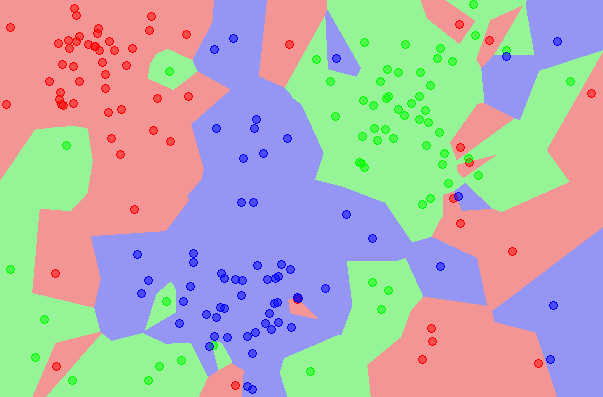
\includegraphics[width=.5\textwidth]{Chapters/03_SimpleML/6_knn/Map1NN.png}
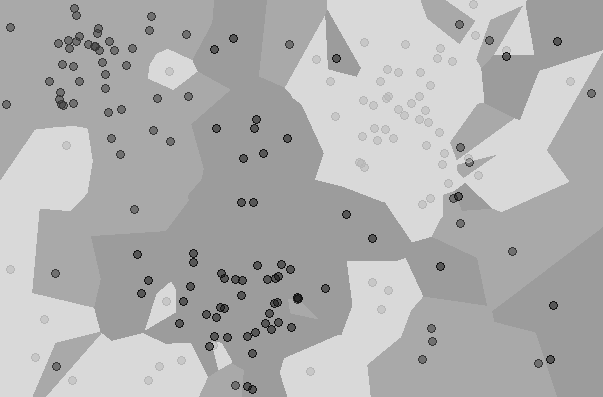
\includegraphics[width=.5\textwidth]{Chapters/03_SimpleML/6_knn/Map1NN_gray.png}
}
\end{figure}
% ******************************************************************************


Hình~\ref{fig:6_1nn} mô tả một bài toán phân loại với ba nhãn: đỏ, lam, lục (xem ảnh màu trong Hình~\ref{fig:6_1nn_c}). Các
hình tròn nhỏ với màu khác nhau thể hiện dữ liệu huấn luyện của các nhãn khác
nhau. Các vùng màu nền khác nhau thể hiện ``lãnh thổ'' của mỗi nhãn. Nhãn của một điểm bất kỳ được xác định dựa trên nhãn của điểm gần nó nhất
trong tập huấn luyện. Trong hình này, có một vài vùng nhỏ xem lẫn vào các
vùng lớn hơn khác màu. Điểm này rất có thể là nhiễu. Các điểm dữ liệu kiểm tra gần khu vực điểm này nhiều khả năng sẽ bị phân loại sai.

Với KNN, mọi điểm trong tập
huấn luyện đều được mô hình mô tả một cách chính xác. Việc này khiến overfitting dễ xảy ra với KNN.

Mặc dù có nhiều hạn chế, KNN vẫn là giải pháp đầu tiên nên nghĩ tới khi giải
quyết một bài toán machine learning. {Khi làm các bài toán machine
learning nói chung, không có mô hình đúng hay sai, chỉ có mô hình cho kết quả
tốt hơn. Chúng ta luôn cần một mô hình đơn giản để giải quyết bài toán, sau đó mới dần tìm cách tăng chất lượng của mô hình.}



% \subsection{Khoảng cách trong không gian vector}

% Trong không gian một chiều, khoảng cách giữa hai điểm là trị tuyệt đối giữa hiệu
% giá trị của hai điểm đó. Trong không gian nhiều chiều, khoảng cách giữa hai điểm
% có thể được định nghĩa bằng nhiều hàm số khác nhau, trong đó độ dài đường thằng
% nổi hai điểm chỉ là một trường hợp đặc biệt trong đó. Nhiều thông tin bổ ích
% (cho Machine Learning) có thể được tìm thấy tại
% \href{http://machinelearningcoban.com/math/#-norms-chuan}{Norms (chuẩn) của
% vector} trong tab \href{http://machinelearningcoban.com/math/}{Math}.




\section{Phân tích toán học}
% Thuật toán KNN rất dễ hiểu nên sẽ phần "Phân tích toán học" này sẽ chỉ có 3 câu.
% Tôi trực tiếp đi vào các ví dụ. Có một điều đáng lưu ý là KNN phải \textit{nhớ}
% tất cả các điểm dữ liệu training, việc này không được lợi về cả bộ nhớ và thời
% gian tính toán - giống như khi cậu bạn của chúng ta không tìm được câu trả lời
% cho câu hỏi cuối cùng.
Không có hàm mất mát hay bài toán tối ưu nào cần thực hiện trong quá trình
huấn luyện KNN. Mọi tính toán được tiến hành ở bước kiểm tra. Vì KNN ra quyết
định dựa trên các điểm gần nhất nên có hai vấn đề ta cần lưu tâm. Thứ nhất,
khoảng cách được định nghĩa như thế nào. Thứ hai, cần phải tính toán khoảng cách
như thế nào cho hiệu quả.

Với vấn đề thứ nhất, mỗi điểm dữ liệu được thể hiện bằng một vector đặc trưng,
khoảng cách giữa hai điểm chính là khoảng cách giữa hai vector đó. Có nhiều loại khoảng cách khác nhau tuỳ vào bài toán, nhưng khoảng cách được sử dụng nhiều nhất là khoảng cách Euclid (xem Mục~\ref{sec:2_norm}).

\index{quy mô lớn -- large-scale}
\index{large-scale -- quy mô lớn}

Vấn đề thứ hai cần được lưu tâm hơn, đặc biệt với {các bài toán có tập huấn
luyện lớn và vector dữ liệu có kích thước lớn}. Giả sử các vector huấn luyện là
các cột của ma trận $\bX\in \R^{d\times N}$ với $d$ và $N$ lớn. KNN sẽ phải tính khoảng cách từ một điểm dữ liệu mới $\bz \in \R^{d}$ đến toàn bộ $N$ điểm
dữ liệu đã cho và chọn ra $K$ khoảng cách nhỏ nhất. Nếu không có cách tính hiệu
quả, khối lượng tính toán sẽ rất lớn.

Tiếp theo, chúng ta cùng thực hiện một vài phân tích toán học để tính các khoảng cách một cách hiệu quả. Ở đây khoảng cách được xem xét là khoảng cách Euclid.
% \subsection{Một cách hiệu quả để tính khoảng cách}
\subsubsection{Khoảng cách từ một điểm tới từng điểm trong một tập hợp}
Khoảng cách Euclid từ một điểm $\bz$ tới một điểm $\bx_i$ trong tập
huấn luyện được định nghĩa bởi $\|\bz - \bx_i\|_2$. Người ta thường dùng bình phương khoảng cách Euclid $\|\bz -\bx_i\|_2^2$ để tránh phép tính căn bậc hai. Việc bình phương này không ảnh hưởng tới thứ tự của các khoảng cách. Để ý rằng
\begin{equation}
\label{eqn:6_dist}
\|\bz - \bx_i\|_2^2 = (\bz - \bx_i)^T(\bz - \bx_i) = \|\bz\|_2^2 +
\|\bx_i\|_2^2 - 2\bx_i^T\bz
\end{equation}
Để tìm ra $\bx_i$ gần với $\bz$ nhất, số hạng đầu tiên
có thể được bỏ qua. Hơn nữa, nếu có nhiều điểm dữ liệu trong tập kiểm tra, các
giá trị $\|\bx_i\|_2^2$ có thể được tính và lưu trước vào bộ nhớ. Khi đó, ta chỉ
cần tính các tích vô hướng $\bx_i^T\bz$.

Để thấy rõ hơn, chúng ta cùng làm một ví dụ trên Python. Trước hết, chọn $d$ và
$N$ là các giá trị lớn và khai báo ngẫu nhiên $\bX$ và $\bz$. Khi lập trình Python, cần lưu ý rằng chiều thứ nhất thường chỉ thứ tự của điểm dữ liệu.
\begin{lstlisting}[language=Python]
from __future__ import print_function
import numpy as np
from time import time # for comparing runing time
d, N = 1000, 10000 # dimension, number of training points
X = np.random.randn(N, d) # N d-dimensional points
z = np.random.randn(d)
\end{lstlisting}

Tiếp theo, ta viết ba hàm số:
\begin{enumerate}

\item \pythoninline{dist_pp(z, x)} tính bình phương khoảng cách Euclid giữa \pythoninline{z} và \pythoninline{x}. Hàm này tính hiệu $\bz - \bx$ rồi lấy bình phương $\ell_2$ norm của nó.


\item \pythoninline{dist_ps_naive(z, X)} tính bình phương khoảng cách giữa
\pythoninline{z} và mỗi {hàng} của \pythoninline{X}. Trong hàm này,
các khoảng cách được xây dựng dựa trên việc tính từng giá trị
\pythoninline{dist_pp(z, X[i])}.

\item \pythoninline{dist_ps_fast(z, X)} tính bình phương khoảng cách giữa
\pythoninline{z} và mỗi {hàng} của \pythoninline{X}, tuy nhiên, kết
quả được tính dựa trên đẳng thức~\eqref{eqn:6_dist}. Ta cần tính tổng bình phương các phần tử của mỗi điểm dữ liệu trong \pythoninline{X} và tính tích \pythoninline{X.dot(z)}
\end{enumerate}

Đoạn code dưới đây thể hiện hai cách tính khoảng cách từ một điểm
\pythoninline{z} tới một tập hợp điểm \pythoninline{X}.
Kết quả và thời gian chạy của mỗi hàm được in ra để so sánh.
% \newpage

\begin{lstlisting}[language=Python]
# naively compute square distance between two vector
def dist_pp(z, x):
    d = z - x.reshape(z.shape) # force x and z to have the same dims
    return np.sum(d*d)

# from one point to each point in a set, naive
def dist_ps_naive(z, X):
    N = X.shape[0]
    res = np.zeros((1, N))
    for i in range(N):
        res[0][i] = dist_pp(z, X[i])
    return res
\end{lstlisting}

\newpage
\begin{lstlisting}[language=Python]
# from one point to each point in a set, fast
def dist_ps_fast(z, X):
    X2 = np.sum(X*X, 1) # square of l2 norm of each X[i], can be precomputed
    z2 = np.sum(z*z) # square of l2 norm of z
    return X2 + z2 - 2*X.dot(z) # z2 can be ignored

t1 = time()
D1 = dist_ps_naive(z, X)
print('naive point2set, running time:', time() - t1, 's')

t1 = time()
D2 = dist_ps_fast(z, X)
print('fast point2set , running time:', time() - t1, 's')
print('Result difference:', np.linalg.norm(D1 - D2))
\end{lstlisting}

\kq
\begin{lstlisting}[language=Python]
naive point2set, running time: 0.0932548046112 s
fast point2set , running time: 0.0514178276062 s
Result difference: 2.11481965531e-11
\end{lstlisting}

Kết quả chỉ ra rằng hàm \pythoninline{dist_ps_fast(z, X)} chạy nhanh hơn gần
gấp đôi so với hàm \pythoninline{dist_ps_naive(z, X)}. Tỉ lệ này còn lớn hơn
khi kích thước dữ liệu tăng lên và \pythoninline{X2} được tính từ trước. Quan trọng hơn, sự chênh lệch nhỏ giữa kết quả của hai cách tính chỉ ra rằng \pythoninline{dist_ps_fast(z, X)} nên được ưu tiên hơn.

\subsubsection{Khoảng cách giữa từng cặp điểm trong hai tập hợp}
Thông thường, tập kiểm tra bao gồm nhiều điểm dữ liệu tạo thành một ma trận
$\bZ$. Ta phải tính từng cặp khoảng cách giữa mỗi điểm trong tập kiểm tra và một
điểm trong tập huấn luyện. Nếu mỗi tập có 1000 phần tử, có một triệu khoảng cách
cần tính. Nếu không có phương pháp tính hiệu quả, thời gian thực hiện sẽ rất dài.

Đoạn code dưới đây thể hiện hai phương pháp tính bình phương khoảng cách giữa
các cặp điểm trong hai tập điểm. Phương pháp thứ nhất sử dụng một vòng
\pythoninline{for} tính khoảng cách từ từng điểm trong tập thứ nhất đến tất cả
các điểm trong tập thứ hai thông qua hàm
\pythoninline{dist_ps_fast(z, X)} ở trên. Phương pháp thứ hai tiếp tục sử
dụng~\eqref{eqn:6_dist} cho trường hợp tổng quát.


\begin{lstlisting}[language=Python]
Z = np.random.randn(100, d)
# from each point in one set to each point in another set, half fast
def dist_ss_0(Z, X):
    M, N = Z.shape[0], X.shape[0]
    res = np.zeros((M, N))
    for i in range(M):
        res[i] = dist_ps_fast(Z[i], X)
    return res
\end{lstlisting}

\par
\par
\begin{lstlisting}[language=Python]
# from each point in one set to each point in another set, fast
def dist_ss_fast(Z, X):
    X2 = np.sum(X*X, 1) # square of l2 norm of each ROW of X
    Z2 = np.sum(Z*Z, 1) # square of l2 norm of each ROW of Z
    return Z2.reshape(-1, 1) + X2.reshape(1, -1) - 2*Z.dot(X.T)

t1 = time()
D3 = dist_ss_0(Z, X)
print('half fast set2set running time:', time() - t1, 's')
t1 = time()
D4 = dist_ss_fast(Z, X)
print('fast set2set  running time', time() - t1, 's')
print('Result difference:', np.linalg.norm(D3 - D4))
\end{lstlisting}
\kq
\begin{lstlisting}[language=Python]
half fast set2set running time: 4.33642292023 s
fast set2set  running time 0.0583250522614 s
Result difference: 9.93586539607e-11
\end{lstlisting}
Điều này chỉ ra rằng hai cách tính cho kết quả chênh lệch nhau không đáng kể.
Trong khi đó \pythoninline{dist_ss_fast(Z, X)} chạy nhanh hơn
\pythoninline{dist_ss_0(Z, X)} nhiều lần.

Khi làm việc trên python, chúng ta có thể sử dụng hàm
\pythoninline{cdist} (\url{https://goo.gl/vYMnmM}) trong
\pythoninline{scipy.spatial.distance}, hoặc hàm
\pythoninline{pairwise_distances} (\url{https://goo.gl/QK6Zyi}) trong
\pythoninline{sklearn.metrics.pairwise}. Các hàm này giúp tính khoảng cách từng
cặp điểm trong hai tập hợp khá hiệu quả. Phần còn lại của chương này sẽ trực
tiếp sử dụng thư viện scikit-learn cho KNN. Việc viết lại thuật toán này không
quá phức tạp khi đã có một hàm tính khoảng cách hiệu quả.

Bạn đọc có thể tham khảo thêm bài báo~\cite{johnson2017billion} về cách thực
hiện KNN trên  và mã nguồn tại
\url{https://github.com/facebookresearch/faiss}.



\section{Ví dụ trên cơ sở dữ liệu Iris}

\begin{figure}[t]
\centering
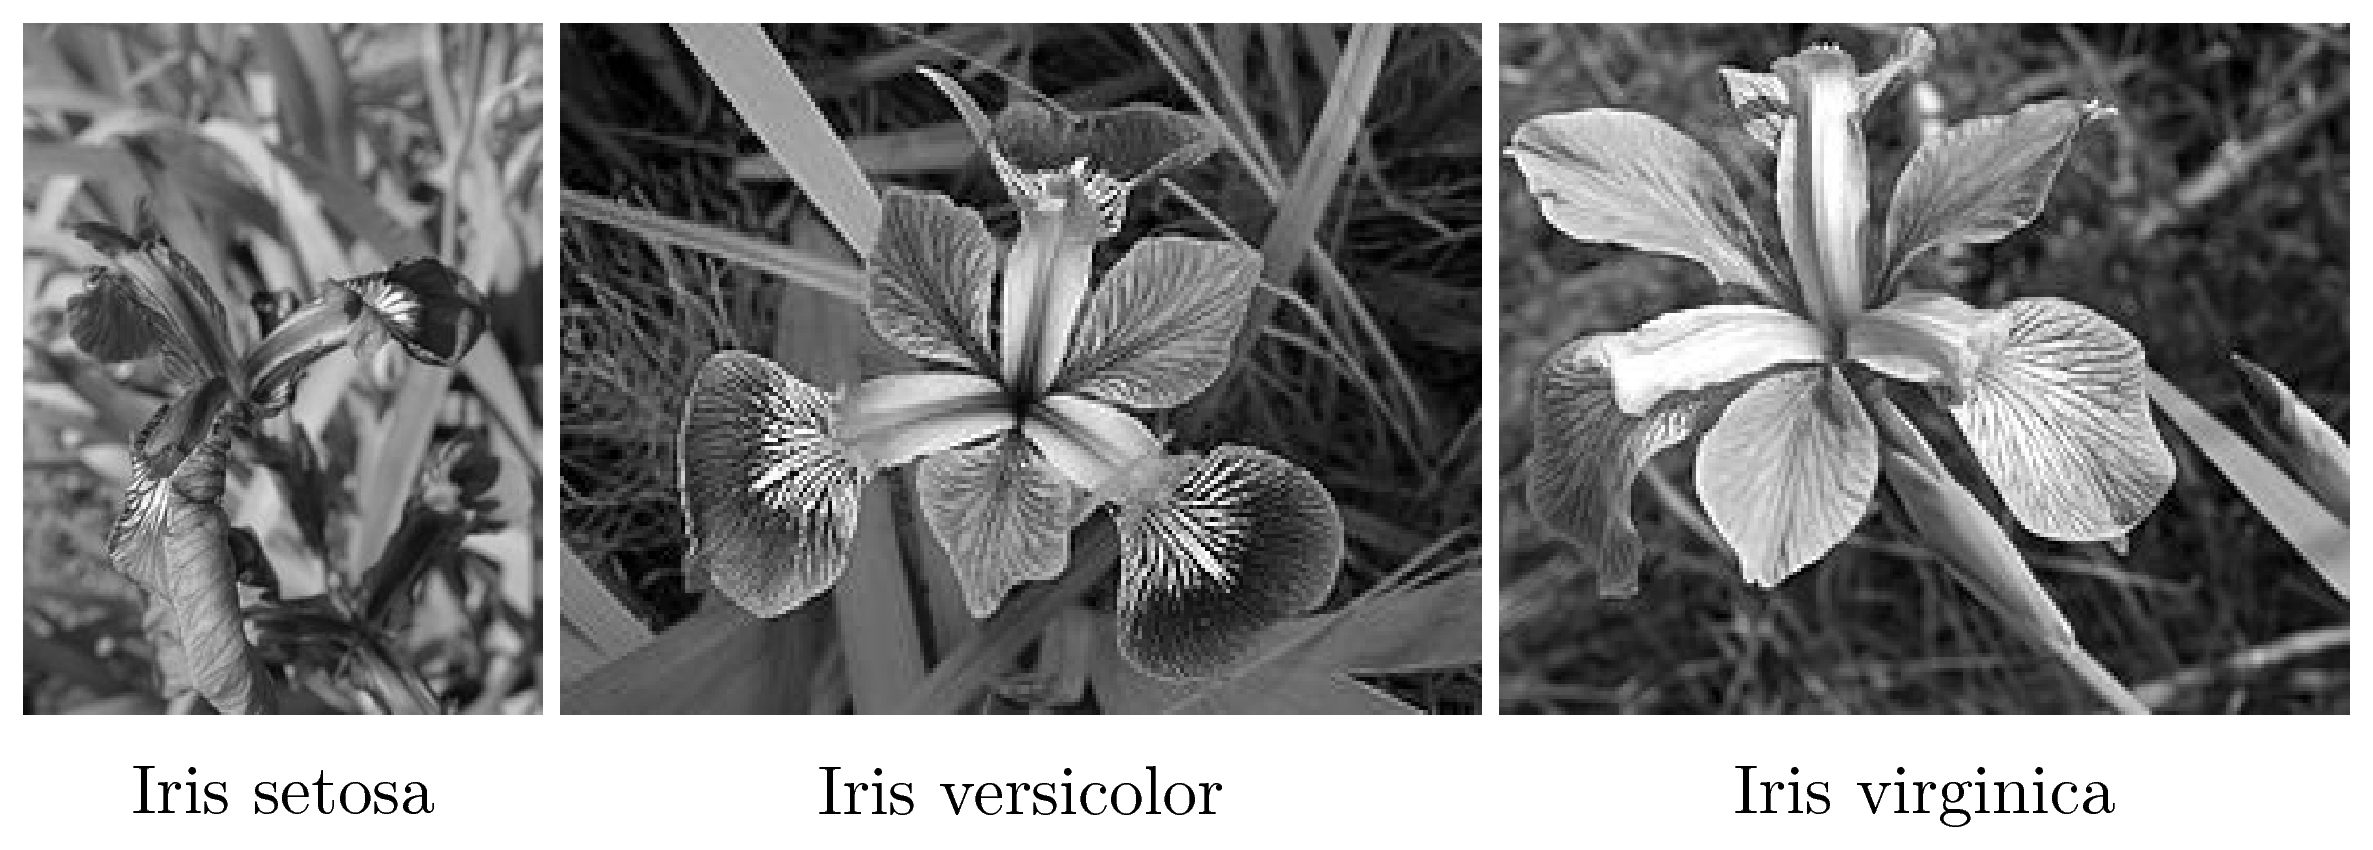
\includegraphics[width = \textwidth]{Chapters/03_SimpleML/6_knn/iris_gray.png}
\caption[]{Ba loại hoa lan trong bộ cơ sở dữ liệu hoa Iris (xem ảnh màu trong Hình~\ref{fig:6_iris_c}).}
\label{fig:6_iris}
\end{figure}


\subsection{Bộ cơ sở dữ liệu hoa Iris}

Bộ dữ liệu hoa Iris (\url{https://goo.gl/eUy83R}) là một bộ dữ liệu nhỏ. Bộ dữ
liệu này bao gồm thông tin của ba nhãn hoa Iris khác nhau: Iris setosa, Iris
virginica và Iris versicolor. Mỗi nhãn chứa thông tin của 50 bông hoa với dữ
liệu là bốn thông tin: chiều dài, chiều rộng đài hoa, và chiều dài,
chiều rộng cánh hoa. Hình~\ref{fig:6_iris} là ví dụ về hình ảnh của ba
loại hoa. Chú ý rằng các điểm dữ liệu không phải là các bức ảnh mà chỉ là một
vector đặc trưng bốn chiếu gồm các thông tin ở trên.

% \begin{figure}[t]
% \centering
%     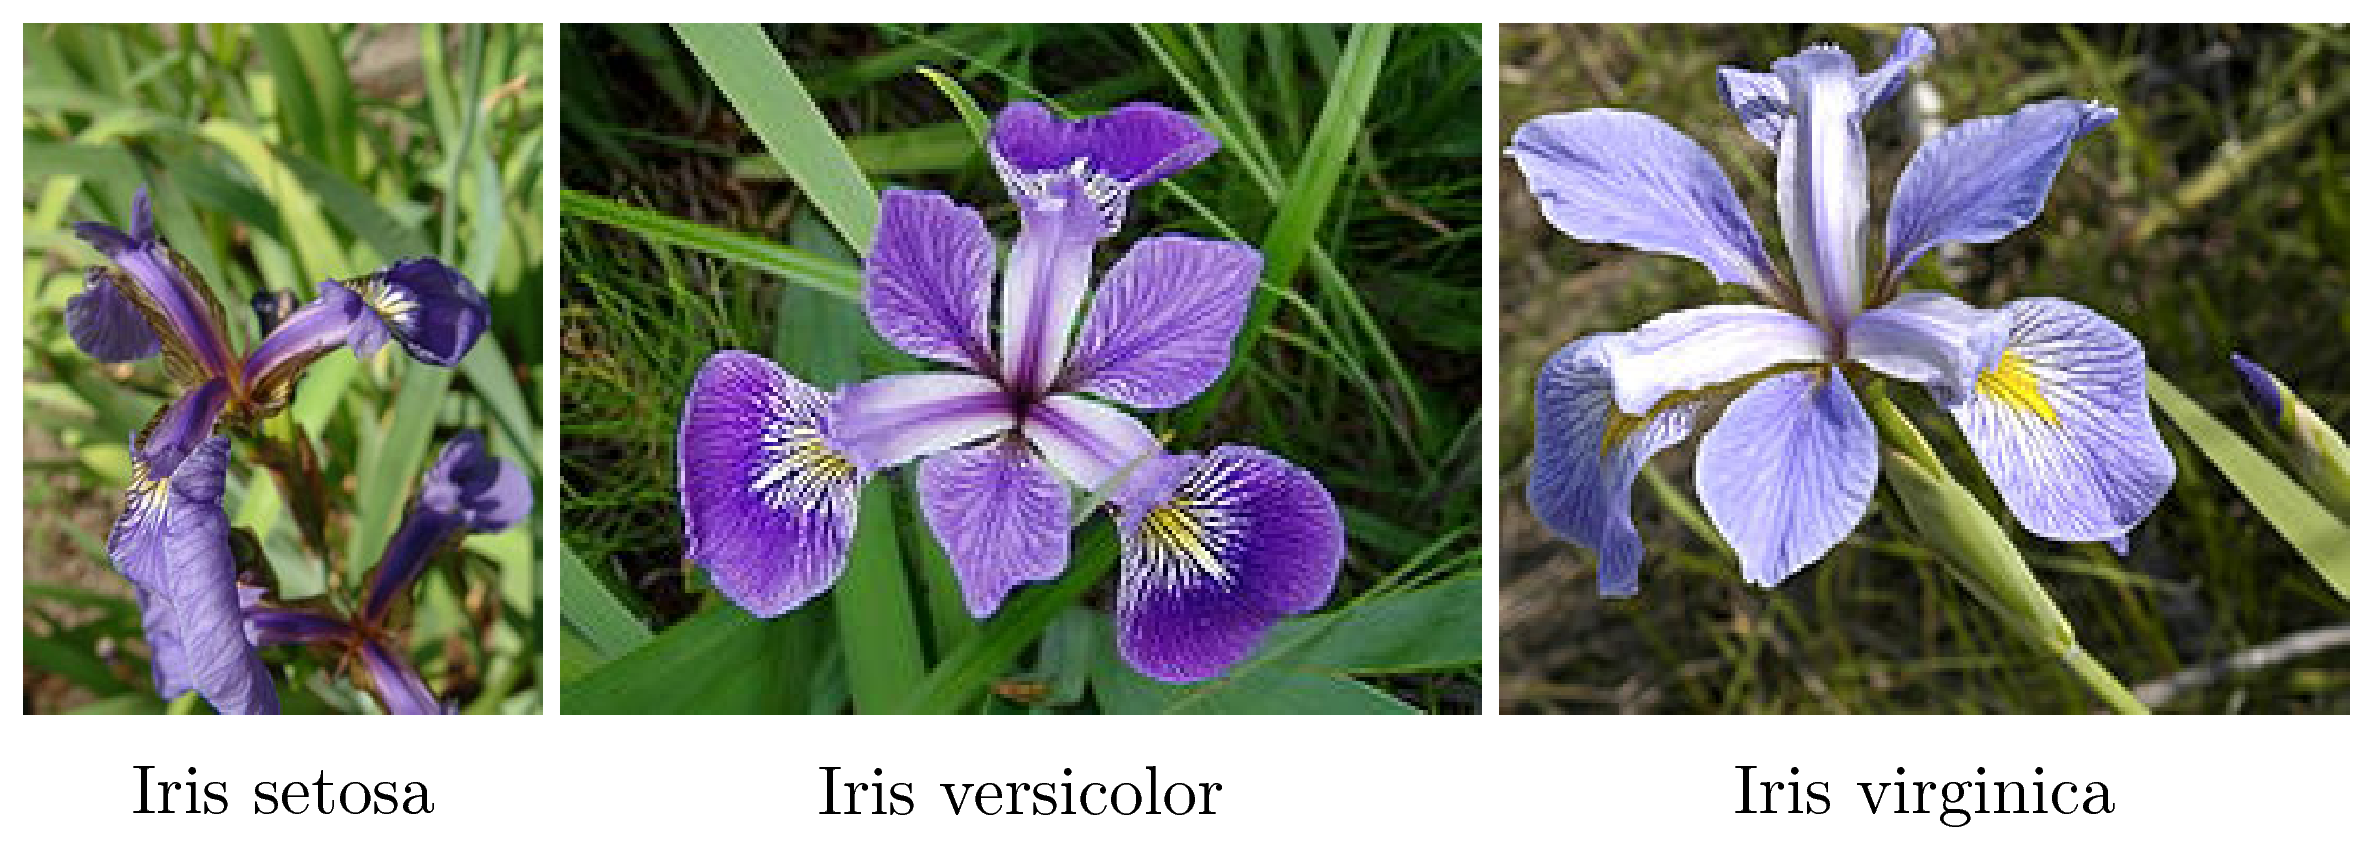
\includegraphics[width = \textwidth]{Chapters/03_SimpleML/6_knn/iris.png}
%     \caption[]{Ba loại hoa lan trong bộ cơ sở dữ liệu hoa Iris.}
%     \label{fig:6_iris}
% \end{figure}

% <div class="imgcap">
% <img src ="/assets/knn/iris.png" align = "center" width="800">
% <div class="thecap"> Ví dụ về Iris flower dataset (Nguồn: <a href = "https://en.wikipedia.org/wiki/Iris_flower_data_set">Wikipedia</a>) <br></div>
% </div>

% Bộ dữ liệu nhỏ này thường được sử dụng trong nhiều thuật toán Machine Learning
% trong các lớp học. Tôi sẽ giải thích lý do không chọn MNIST vào phần sau.



\subsection{Thí nghiệm}


Trong phần này, 150 điểm dữ liệu được tách thành tập huấn luyện và tập kiểm tra.
KNN dựa vào trông tin trong tập huấn luyện để dự đoán mỗi dữ liệu trong tập kiểm
tra tương ứng với loại hoa nào. Kết quả này được đối chiếu với đầu ra thực sự
để đánh giá hiệu quả của KNN.

Trước tiên, chúng ta cần khai báo vài thư viện. Bộ dữ liệu hoa Iris có sẵn trong
thư viện scikit-learn.

\begin{lstlisting}[language=Python]
from __future__ import print_function
import numpy as np
from sklearn import neighbors, datasets
from sklearn.model_selection import train_test_split # for splitting data
from sklearn.metrics import accuracy_score      # for evaluating results

iris = datasets.load_iris()
iris_X = iris.data
iris_y = iris.target
\end{lstlisting}

Tiếp theo, 20 mẫu dữ liệu được lấy ra ngẫu nhiên tạo thành tập huấn luyện, 130 mẫu còn lại được dùng để kiểm tra.
% \newpage

\begin{lstlisting}[language=Python]
print('Labels:', np.unique(iris_y))

# split train and test
np.random.seed(7)
X_train, X_test, y_train, y_test = train_test_split(
    iris_X, iris_y, test_size=130)
print('Training size:', X_train.shape[0], ', test size:', X_test.shape[0])
\end{lstlisting}
\begin{lstlisting}
Labels: [0 1 2]
Training size: 20 , test size: 130
\end{lstlisting}

Dòng \pythoninline{np.random.seed(7)} để đảm bảo kết quả chạy ở các lần khác nhau là giống nhau. Có thể thay 7 bằng một số tự
nhiên 32 bit bất kỳ.

\subsubsection{Kết quả với 1NN}
Tới đây, ta trực tiếp sử dụng thư viện scikit-learn cho KNN. Xét ví dụ đầu tiên
với $K = 1$.

\begin{lstlisting}[language=Python]
model = neighbors.KNeighborsClassifier(n_neighbors = 1, p = 2)
model.fit(X_train, y_train)
y_pred = model.predict(X_test)
print("Accuracy of 1NN: %.2f %%" %(100*accuracy_score(y_test, y_pred)))
\end{lstlisting}
\kq
\begin{lstlisting}[language=Python]
Accuracy of 1NN: 92.31 %
\end{lstlisting}

Kết quả thu được là 92.31\% (tỉ lệ số mẫu được phân loại chính xác trên tổng số
mẫu). Ở đây, \pythoninline{n_neighbors = 1} chỉ ra rằng chỉ điểm gần nhất được
lựa chọn, tức $K = 1$, \pythoninline{p = 2} chính là $\ell_2$ norm để tính
khoảng cách. Bạn đọc có thể thử với \pythoninline{p = 1} tương ứng với khoảng
cách $\ell_1$ norm.





% \subsubsection{Tách training và test sets}
% Giả sử chúng ta muốn dùng 50 điểm dữ liệu cho test set, 100 điểm còn lại cho
% training set. Scikit-learn có một hàm số cho phép chúng ta ngẫu nhiên lựa chọn
% các điểm này, như sau:


% \begin{lstlisting}[language=Python]
% from sklearn.model_selection import train_test_split
% X_train, X_test, y_train, y_test = train_test_split(
%      iris_X, iris_y, test_size=50)

% print "Training size: %d" %len(y_train)
% print "Test size    : %d" %len(y_test)
% \end{lstlisting}
% \begin{lstlisting}[language=Python]
% Training size: 100
% Test size    : 50
% \end{lstlisting}


% Sau đây, tôi trước hết xét trường hợp đơn giản K = 1, tức là với mỗi điểm test
% data, ta chỉ xét 1 điểm training data gần nhất và lấy label của điểm đó để dự
% đoán cho điểm test này.


% \begin{lstlisting}[language=Python]
% clf = neighbors.KNeighborsClassifier(n_neighbors = 1, p = 2)
% clf.fit(X_train, y_train)
% y_pred = clf.predict(X_test)

% print "Print results for 20 test data points:"
% print "Predicted labels: ", y_pred[20:40]
% print "Ground truth    : ", y_test[20:40]
% \end{lstlisting}
% \begin{lstlisting}[language=Python]
% Print results for first 20 test data points:
% Predicted labels:  [2 1 2 2 1 2 2 0 2 0 2 0 1 0 0 2 2 0 2 0]
% Ground truth    :  [2 1 2 2 1 2 2 0 2 0 1 0 1 0 0 2 1 0 2 0]
% \end{lstlisting}

% <a name = "ground-truth"></a>
% Kết quả cho thấy label dự đoán gần giống với label thật của test data, chỉ có 2
% điểm trong số 20 điểm được hiển thị có kết quả sai lệch. Ở đây chúng ta làm quen
% với khái niệm mới: \textit{ground truth}. Một cách đơn giản, \textit{ground
% truth} chính là nhãn/label/đầu ra \textit{thực sự} của các điểm trong test data.
% Khái niệm này được dùng nhiều trong Machine Learning, hy vọng lần tới các bạn
% gặp thì sẽ nhớ ngay nó là gì.



% \subsubsection{Phương pháp đánh giá (evaluation method)}
% Để đánh giá độ chính xác của thuật toán KNN classifier này, chúng ta xem xem có
% bao nhiêu điểm trong test data được dự đoán đúng. Lấy số lượng này chia cho tổng
% số lượng trong tập test data sẽ ra độ chính xác. Scikit-learn cung cấp hàm số
% \href{http://scikit-learn.org/stable/modules/generated/sklearn.metrics.accuracy_score.html}{\pythoninline{accuracy_score}} để
% thực hiện công việc này.


% \begin{lstlisting}[language=Python]
% from sklearn.metrics import accuracy_score
% print "Accuracy of 1NN: %.2f %%" %(100*accuracy_score(y_test, y_pred))
% \end{lstlisting}

% \begin{lstlisting}[language=Python]
% Accuracy of 1NN: 94.00 %
% \end{lstlisting}


% 1NN đã cho chúng ta kết quả là 94\%, không tệ! Chú ý rằng đây là một cơ sở dữ
% liệu dễ vì chỉ với dữ liệu ở hai cột cuối cùng, chúng ta đã có thể suy ra quy
% luật. Trong ví dụ này, tôi sử dụng \pythoninline{p = 2} nghĩa là khoảng cách ở
% đây được tính là khoảng cách theo
% \href{http://machinelearningcoban.com/math/#norm2}{$\ell_2$ norm}. Các bạn cũng có thể
% thử bằng cách thay \pythoninline{p = 1} cho
% \href{http://machinelearningcoban.com/math/#norm0}{norm 1}, hoặc các gía trị
% \pythoninline{p} khác cho norm khác. (Xem thêm
% \href{http://scikit-learn.org/stable/modules/generated/sklearn.neighbors.KNeighborsClassifier.html}{sklearn.neighbors.KNeighborsClassifier})

\subsubsection{Kết quả với 7NN}
\index{bầu chọn đa số -- major voting}
\index{major voting -- bầu chọn đa số}
Như đã đề cập, 1NN rất dễ gây ra overfitting. Để hạn chế việc này, ta có thể
tăng lượng điểm lân cận lên, ví dụ bảy điểm, kết quả được xác định dựa trên đa
số.

\begin{lstlisting}[language=Python]
model = neighbors.KNeighborsClassifier(n_neighbors = 7, p = 2)
model.fit(X_train, y_train)
y_pred = model.predict(X_test)

print("Accuracy of 7NN with major voting: %.2f %%"\ 
     %(100*accuracy_score(y_test, y_pred)))

\end{lstlisting}
\kq
\begin{lstlisting}[language=Python]
Accuracy of 7NN with major voting: 93.85 %
\end{lstlisting}

Nhận thấy rằng khi sử dụng nhiều điểm lân cận hơn, độ chính xác đã tăng lên. Phương pháp dựa trên đa số trong lân cận còn được gọi là \textit{bầu chọn đa số}.

% \begin{lstlisting}[language=Python]
% clf = neighbors.KNeighborsClassifier(n_neighbors = 10, p = 2)
% clf.fit(X_train, y_train)
% y_pred = clf.predict(X_test)

% print "Accuracy of 10NN with major voting: %.2f %%" %(100*accuracy_score(y_test, y_pred))
% \end{lstlisting}
% \begin{lstlisting}[language=Python]
% Accuracy of 10NN with major voting: 98.00 %
% \end{lstlisting}


% Kết quả đã tăng lên 98%, rất tốt!



\subsubsection{Đánh trọng số cho các điểm lân cận}
Trong kỹ thuật bầu chọn đa số phía trên, các điểm trong bảy điểm gần nhất đều có
vai trò như nhau và giá trị ``lá phiếu'' của mỗi điểm này cũng như nhau. Cách bầu chọn này có thể thiếu công bằng vì các điểm gần hơn nên có tầm ảnh hưởng lớn hơn. Để thực hiện việc này, ta chỉ cần đánh trọng số khác nhau cho từng điểm trong bảy điểm gần nhất này. Cách
đánh trọng số phải thoả mãn điều kiện điểm lân cận hơn được đánh trọng số cao hơn. Một cách đơn giản là lấy nghịch đảo của khoảng
cách tới điểm lân cận. Trong trường hợp tồn tại khoảng cách bằng không, tức điểm kiểm tra trùng với một điểm huấn luyện, ta trực tiếp lấy đầu ra của điểm huấn luyện đó.

Để thực hiện việc này trong scikit-learn, ta chỉ cần gán
\pythoninline{weights = 'distance'}. Giá trị mặc định của
\pythoninline{weights} là \pythoninline{'uniform'}, tương ứng với việc coi tất
cả các điểm lân cận có giá trị bằng nhau như trong bầu chọn đa số.

\begin{lstlisting}[language=Python]
model = neighbors.KNeighborsClassifier(n_neighbors = 7, p = 2, \
weights = 'distance')
model.fit(X_train, y_train)
y_pred = model.predict(X_test)

print("Accuracy of 7NN (1/distance weights): %.2f %%" %(100*accuracy_score(y_test, y_pred)))
\end{lstlisting}
\kq
\begin{lstlisting}[language=Python]
Accuracy of 7NN (1/distance weights): 94.62 %
\end{lstlisting}
% \begin{lstlisting}[language=Python]
% clf = neighbors.KNeighborsClassifier(n_neighbors = 10, p = 2, weights = 'distance')
% clf.fit(X_train, y_train)
% y_pred = clf.predict(X_test)

% print "Accuracy of 10NN (1/distance weights): %.2f %%" %(100*accuracy_score(y_test, y_pred))
% \end{lstlisting}
% \begin{lstlisting}[language=Python]
% Accuracy of 10NN (1/distance weights): 100.00 %
% \end{lstlisting}


Độ chính xác tiếp tục được tăng lên.

\subsubsection{KNN với trọng số tự định nghĩa}
Ngoài hai cách đánh trọng số \pythoninline{weights =
`uniform'} và \pythoninline{weights = `distance'}, scikit-learn còn cung
cấp cách đánh trọng số tùy chọn. Ví dụ, một cách
đánh trọng số phổ biến khác thường được dùng là
\begin{equation*}
w_i = \exp \left( \frac{-\|\mathbf{z} - \mathbf{x}_i\|_2^2}{\sigma^2}
\right)
\end{equation*}
trong đó $w_i$ là trọng số của điểm gần thứ $i$ ($\bx_i$) của điểm dữ liệu
đang xét $\mathbf{z}$, $\sigma$ là một số dương. Hàm số này cũng
thỏa mãn
điều kiện điểm càng gần $\mathbf{x}$ thì trọng số càng cao (cao nhất bằng 1).
Với hàm số này, ta có thể lập trình như sau:


\begin{lstlisting}[language=Python]
def myweight(distances):
sigma2 = .4 # we can change this number
return np.exp(-distances**2/sigma2)

model = neighbors.KNeighborsClassifier(
    n_neighbors = 7, p = 2, weights = myweight)
model.fit(X_train, y_train)
y_pred = model.predict(X_test)

print("Accuracy of 7NN (customized weights): %.2f %%"\
      %(100*accuracy_score(y_test, y_pred)))
\end{lstlisting}
\kq
\begin{lstlisting}[language=Python]
Accuracy of 7NN (customized weights): 95.38 %
\end{lstlisting}

Kết quả tiếp tục tăng lên một chút. Với từng bài toán, chúng ta có thể
thay các thuộc tính của KNN bằng các giá trị khác nhau và chọn ra giá trị tốt
nhất thông qua xác thực chéo (xem Mục~\ref{ssec:crosvalid}).

% Trong trường hợp này, kết quả tương đương với kỹ thuật major voting. Để đánh giá
% chính xác hơn kết quả của KNN với K khác nhau, cách định nghĩa khoảng cách khác
% nhau và cách đánh trọng số khác nhau, chúng ta cần thực hiện quá trình trên với
% nhiều cách chia dữ liệu \textit{training} và \textit{test} khác nhau rồi lấy kết
% quả trung bình, vì rất có thể dữ liệu phân chia trong 1 trường hợp cụ thể là rất
% tốt hoặc rất xấu (bias). Đây cũng là cách thường được dùng khi đánh giá hiệu
% năng của một thuật toán cụ thể nào đó.



\section{Thảo luận}



\subsection{KNN cho bài toán hồi quy}
Với bài toán hồi quy, chúng ta cũng hoàn toàn có thể sử dụng phương pháp
tương tự: đầu ra của một điểm được xác định dựa trên đầu ra của các điểm lân cận
và khoảng cách tới chúng. Giả sử $\bx_1, \dots, \bx_K$ là $K$ điểm lân cận của
một điểm dữ liệu $\bz$ với đầu ra tương ứng là $y_1, \dots, y_K$. Giả sử các
trọng số ứng với các lân cận này là $w_1, \dots, w_K$. Kết quả dự đoán
đầu ra của $\bz$ có thể được xác định bởi
\begin{equation}
\displaystyle
\frac{w_1 y_1 + w_2 y_2 + \dots + w_Kw_K}{w_1 + w_2 + \dots + w_K}
\end{equation}
Hình~\ref{fig:6_knn_reg} là một ví dụ về KNN cho hồi quy với $K = 5$,
sử dụng hai cách đánh trọng số khác nhau. Ta có thể thấy rằng
\pythoninline{weights = 'distance'} có xu hướng gây ra overfitting.

\begin{figure}[t]
\centering
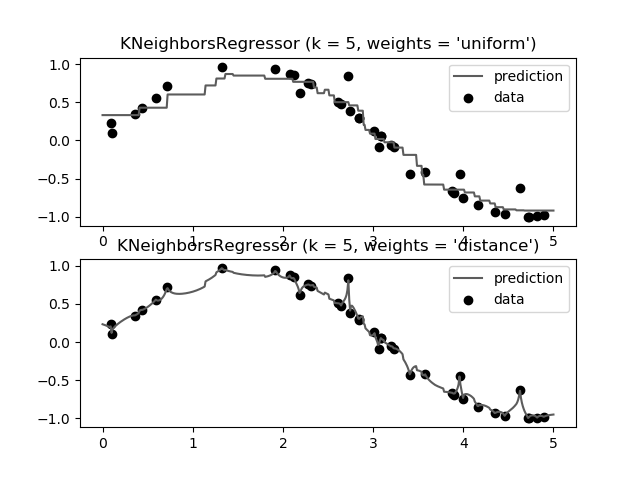
\includegraphics[width =
.7\textwidth]{Chapters/03_SimpleML/6_knn/sphx_glr_plot_regression_001_gray.png}
\caption[]{KNN cho bài toán hồi quy (Nguồn:
\textit{Nearest neighbors regression -- scikit-learn} -- \url{https://goo.gl/9VyBF3}).}
\label{fig:6_knn_reg}
\end{figure}
% \begin{figure}[t]
%     % caption on side



%     \floatbox[{\capbeside\thisfloatsetup{capbesideposition={right,top},capbesidewidth=3cm}}]{figure}[\FBwidth]
%     {\caption{
%     KNN cho bài toán Regression (Nguồn:
%     \href{https://goo.gl/9VyBF3}{Nearest Neighbors regression  --  scikit-learn}).
%     }
%     \label{fig:6_knn_reg}}
%     { % figure here
%     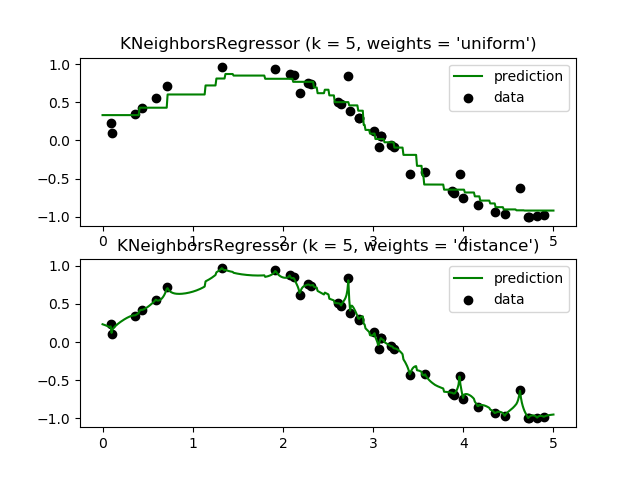
\includegraphics[width=.75\textwidth]{Chapters/03_SimpleML/6_knn/sphx_glr_plot_regression_001.png}
%     }
% \end{figure}


% <div class="imgcap">
% <img src ="http://scikit-learn.org/stable/_images/sphx_glr_plot_regression_001.png" align = "center">
% <div class="thecap"> KNN cho bài toán Regression  (Nguồn: <a href = "http://scikit-learn.org/stable/auto_examples/neighbors/plot_regression.html#sphx-glr-auto-examples-neighbors-plot-regression-py">Nearest Neighbors regression</a>) <br></div>
% </div>



% \subsection{Chuẩn hóa dữ liệu}
% Khi có một thuộc tính trong vector đặc trưng lớn hơn các thuộc tính khác rất
% nhiều, chẳng hạn ví dụ thay vì đo bằng cm thì một kết quả lại tính bằng mm,
% khoảng cách giữa các điểm sẽ phụ thuộc vào thuộc tính này rất nhiều. Để có được
% kết quả chính xác hơn, một kỹ thuật thường được dùng là \textit{Data
% Normalization} (chuẩn hóa dữ liệu) để đưa các thuộc tính có đơn vị đo khác nhau
% về cùng một khoảng giá trị, thường là từ 0 đến 1, trước khi thực hiện KNN. Có
% nhiều kỹ thuật chuẩn hóa khác nhau, các bạn sẽ được thấy khi tiếp tục theo dõi
% Blog này. Các kỹ thuật chuẩn hóa được áp dụng với không chỉ KNN mà còn với hầu
% hết các thuật toán khác.



% \subsection{Sử dụng các phép đo khoảng cách khác nhau}
% Ngoài norm 1 và $\ell_2$ norm tôi giới thiệu trong bài này, còn rất nhiều các khoảng
% cách khác nhau có thể được dùng. Một ví dụ đơn giản là đếm số lượng thuộc tính
% khác nhau giữa hai điểm dữ liệu. Số này càng nhỏ thì hai điểm càng gần nhau. Đây
% chính là \href{http://machinelearningcoban.com/math/#norm0}{giả chuẩn 0} mà tôi đã
% giới thiệu trong Tab \href{http://machinelearningcoban.com/math/}{Math}.



\subsection{Ưu điểm của KNN}
% Ưu điểm
\begin{itemize}
\item Độ phức tạp tính toán của quá trình huấn luyện gần như bằng 0. Việc tính bình phương $\ell_2$ norm của mỗi điểm dữ liệu huấn luyện có thể được thực hiện trước trong bước này.

\item Việc dự đoán kết quả của dữ liệu mới tương đối đơn giản sau khi đã xác
định được các điểm lân cận.

\item KNN không không cần giả sử về phân phối của từng nhãn.
\end{itemize}



\subsection{Nhược điểm của KNN}
% Nhược điểm:
\begin{itemize}
\item KNN nhạy cảm với nhiễu khi $K$ nhỏ.

\item Khi sử dụng KNN, phần lớn tính toán nằm ở pha
kiểm tra. Trong đó việc tính khoảng cách tới {từng} điểm dữ liệu
huấn luyện tốn nhiều thời gian, đặc biệt là với các cơ sở dữ
liệu có số chiều lớn và có nhiều điểm dữ liệu. $K$ càng lớn thì độ phức
tạp càng cao. Ngoài ra, việc lưu toàn bộ dữ liệu trong bộ nhớ cũng
ảnh hưởng tới hiệu năng của KNN.

\end{itemize}


% \subsection{Tăng tốc cho KNN}
% Ngoài việc tính toán khoảng cách từ một điểm test data đến tất cả các điểm trong
% traing set (Brute Force), có một số thuật toán khác giúp tăng tốc việc tìm kiếm
% này. Bạn đọc có thẻ tìm kiếm thêm với hai từ khóa:
% \href{http://pointclouds.org/documentation/tutorials/kdtree_search.php}{K-D
% Tree} và \href{https://en.wikipedia.org/wiki/Ball_tree}{Ball Tree}. Tôi xin dành
% phần này cho độc giả tự tìm hiểu, và sẽ quay lại nếu có dịp. Chúng ta vẫn còn
% những thuật toán quan trọng hơn khác cần nhiều sự quan tâm hơn.


% \subsection{Try this yourself}

% Tôi có viết một đoạn code ngắn để thực hiện việc Classification cho cơ sở dữ
% liệu
% \href{http://machinelearningcoban.com/2017/01/04/kmeans2/#bo-co-so-du-lieu-mnist}{MNIST}.
% Các bạn hãy download toàn bộ bộ dữ liệu này về vì sau này chúng ta còn dùng
% nhiều, chạy thử, comment kết quả và nhận xét của các bạn vào phần comment bên
% dưới. Để trả lời cho câu hỏi vì sao tôi không chọn cơ sở dữ liệu này làm ví dụ,
% bạn đọc có thể tự tìm ra đáp án khi chạy xong đoạn code này.

% Enjoy!


% \begin{lstlisting}[language=Python]
% # %reset
% import numpy as np
% from mnist import MNIST # require `pip install python-mnist`
% # https://pypi.python.org/pypi/python-mnist/

% import matplotlib.pyplot as plt
% from sklearn import neighbors
% from sklearn.metrics import accuracy_score
% import time

% # you need to download the MNIST dataset first
% # at: http://yann.lecun.com/exdb/mnist/
% mndata = MNIST('../MNIST/') # path to your MNIST folder
% mndata.load_testing()
% mndata.load_training()
% X_test = mndata.test_images
% X_train = mndata.train_images
% y_test = np.asarray(mndata.test_labels)
% y_train = np.asarray(mndata.train_labels)


% start_time = time.time()
% clf = neighbors.KNeighborsClassifier(n_neighbors = 1, p = 2)
% clf.fit(X_train, y_train)
% y_pred = clf.predict(X_test)
% end_time = time.time()
% print "Accuracy of 1NN for MNIST: %.2f %%" %(100*accuracy_score(y_test, y_pred))
% print "Running time: %.2f (s)" % (end_time - start_time)
% \end{lstlisting}


% \subsection{Source code}


\subsection{Đọc thêm}

% 1. \href{http://scikit-learn.org/stable/modules/generated/sklearn.neighbors.NearestNeighbors.html#sklearn.neighbors.NearestNeighbors}{sklearn.neighbors.NearestNeighbors}

% 2. \href{http://scikit-learn.org/stable/modules/generated/sklearn.model_selection.train_test_split.html}{sklearn.model\_selection.train\_test\_split}

% 3.
\begin{enumerate}
\item \textit{Tutorial To Implement k-Nearest Neighbors in Python From
Scratch} (\url{https://goo.gl/J78Qso}).

\item Mã nguồn cho chương này có thể được tìm thấy tại \url{https://goo.gl/asF58Q}.

\end{enumerate}

%!TEX root = ../../book_ML.tex
\chapter{Phân cụm $K$-means}
\index{phân cụm $K$-means -- $K$-means clustering}
\index{$K$-means clustering -- phân cụm $K$-means}
\label{cha:kmeans}
\section{Giới thiệu}
Trong Chương~\ref{cha:linear_regression} và, \ref{cha:knn}, chúng ta đã làm quen
các thuật toán học có giám sát. Trong chương này, một thuật toán đơn giản của
học không giám sát sẽ được trình bày. Thuật toán này có tên là \textit{phân cụm
$K$-means} (\textit{$K$-means clustering}).

Trong phân cụm $K$-means, ta không biết nhãn của từng
điểm dữ liệu. Mục đích là làm thể nào để phân dữ liệu thành các cụm (cluster)
khác nhau sao cho dữ liệu trong cùng một cụm có những tính chất giống nhau.

\textbf{Ví dụ:} Một công ty muốn tạo ra một chính sách ưu đãi cho những nhóm
khách hàng khác nhau dựa trên sự tương tác giữa mỗi khách hàng với công ty đó
(số năm là khách hàng, số tiền khách hàng đã chi trả cho công ty, độ tuổi, giới
tính, thành phố, nghề nghiệp,...). Giả sử công ty có dữ liệu của khách hàng
nhưng phân cụm. Phân cụm $K$-means là một thuật toán có thể giúp thực hiện
công việc này. Sau khi phân cụm, nhân viên công ty có thể quyết định mỗi
nhóm tương ứng với nhóm khách hàng nào. Phần việc cuối cùng này cần sự can thiệp
của con người, nhưng lượng công việc đã được rút gọn đi đáng kể.

\index{cụm -- cluster}
\index{cluster -- cụm}

Một nhóm/cụm có thể được định nghĩa là tập hợp các điểm có
vector đặc trưng gần nhau. Việc tính toán khoảng cách có thể phụ thuộc vào từng loại dữ liệu, trong đó khoảng cách Euclid được sử dụng phổ biến nhất. Trong chương này, các tính toán được thực hiện dựa trên khoảng cách Euclid. Tuy nhiên, quy trình thực hiện thuật toán có thể được áp dụng cho các loại khoảng cách khác.

% ******************************************************************************
\begin{figure}[t]
% caption on side
\floatbox[{\capbeside\thisfloatsetup{capbesideposition={right,top},capbesidewidth=6cm}}]{figure}[\FBwidth]
{\caption{
Ví dụ với ba cụm dữ liệu trong không gian hai chiều.
}
\label{fig:4_1}}
{ % figure here
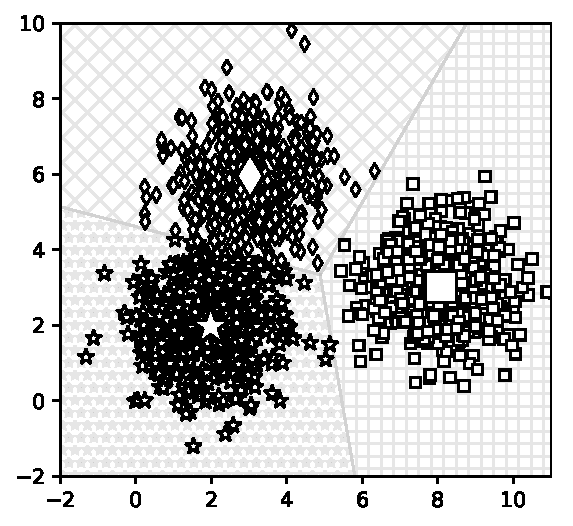
\includegraphics[width=.5\textwidth]{ebookML_src/src/kmeans/ex_5notitle.pdf}
% 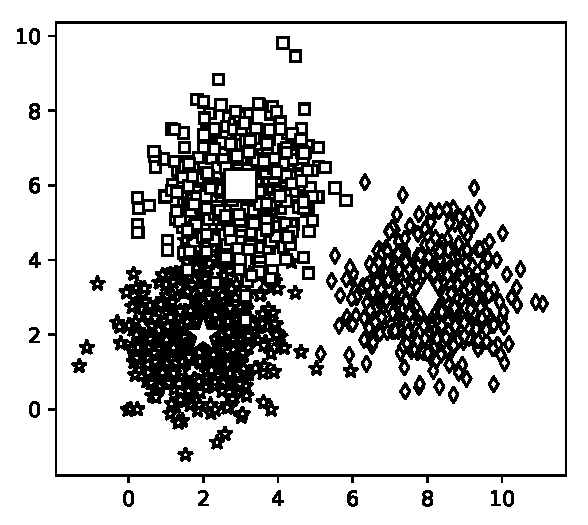
\includegraphics[width=.5\textwidth]{ebookML_src/src/kmeans/data.pdf}
}
\end{figure}
% ******************************************************************************
\index{phân cụm $K$-means -- $K$-means clustering!tâm cụm -- centroid}
\index{$K$-means clustering -- phân cụm $K$-means!centroid -- tâm cụm}

Hình~\ref{fig:4_1} là một ví dụ về dữ liệu được phân vào ba cụm. Giả sử mỗi cụm
có một điểm đại diện được gọi là \textit{tâm cụm}, được minh hoạ bởi các điểm
màu trắng lớn. Mỗi điểm thuộc vào cụm có tâm gần nó nhất. Tới đây, chúng ta có
một bài toán thú vị: {Trên vùng biển hình chữ nhật có ba đảo hình thoi, hình
vuông và sao năm cánh lớn màu trắng như Hình~\ref{fig:4_1}. Một điểm trên biển
được gọi là thuộc lãnh hải của một đảo nếu nó nằm gần đảo này hơn so với hai đảo
còn lại. Hãy xác định ranh giới lãnh hải giữa các đảo.}

% \index{hyperpolygon -- siêu đa diện}
Cũng trên Hình~\ref{fig:4_1}, các vùng với nền khác nhau biểu thị lãnh hải của
mỗi đảo. Có thể thấy rằng đường phân định giữa các lãnh hải có dạng đường
thẳng. Chính xác hơn, chúng là đường trung trực của các cặp đảo gần nhau. Vì
vậy, lãnh hải của một đảo sẽ là một hình đa giác. Cách phân chia dựa trên khoảng
cách tới điểm gần nhất này trong toán học được gọi là Voronoi
diagram\footnote{\textit{Vonoroi diagram -- Wikipedia}
(\url{https://goo.gl/xReCW8}).}. Trong không gian ba chiều, lấy ví dụ là các
hành tinh, \textit{lãnh không} của mỗi hành tinh sẽ là một đa diện. Trong không
gian nhiều chiều hơn, chúng ta sẽ có những \textit{siêu đa diện}.

% Quay lại với bài toán phân cụm và cụ thể là thuật toán phân cụm $K$-means,
% chúng ta cùng thảo luận cơ sở toán học, cách xây dựng và tối ưu hàm mất mát của
% nó.


% chúng ta cần một chút phân tích toán học trước khi đi tới phần
% \href{http://machinelearningcoban.com#tom-tat-thuat-toan}{tóm tắt thuật toán} ở
% phần dưới. Nếu bạn không muốn đọc quá nhiều về toán, bạn có thể bỏ qua phần này.
% (\textit{Tốt nhất là đừng bỏ qua, bạn sẽ tiếc đấy}).

\section{Phân tích toán học }

Mục đích cuối cùng của thuật toán phân cụm $K$-means là từ dữ liệu đầu vào và số
lượng cụm cần tìm, hãy xác định tâm mỗi cụm và phân các điểm dữ liệu vào cụm
tương ứng. Giả sử thêm rằng mỗi điểm dữ liệu chỉ thuộc đúng một cụm.


% \subsection{Một số ký hiệu toán học}
Giả sử $N$ điểm dữ liệu trong tập huấn luyện được ghép lại thành ma trận $ \mathbf{X} =
[\mathbf{x}_1, \mathbf{x}_2, \dots,
\mathbf{x}_N] \in \mathbb{R}^{d \times N}$ và $K < N$ là số cụm được xác định trước. Ta cần tìm các tâm cụm $ \mathbf{m}_1, \mathbf{m}_2,
\dots, \mathbf{m}_K \in \mathbb{R}^{d \times 1}$ và nhãn của mỗi điểm dữ liệu.
Ở đây, mỗi cụm được đại diển bởi một nhãn, thường là một số tự nhiên từ 1
đến $K$. Nhắc lại rằng các điểm dữ liệu trong bài toán phân cụm $K$-means ban
đầu không có nhãn cụ thể.

\index{mã hoá one-hot -- one-hot coding}
\index{one-hot coding -- mã hoá one-hot}
Với mỗi điểm dữ liệu $\bx_i$, ta cần tìm nhãn $y_i = k$ của nó, ở đây $k\in
\{1, 2, \dots, K\}$. Nhãn của một điểm cũng thường được biểu diễn dưới dạng một
vector hàng $K$ phần tử $\by_i \in \R^{1\times K}$, trong đó tất cả các phần tử
của $\by_i$ bằng 0 trừ phần tử ở vị trí thứ $k$ bằng 1. Cách biểu diễn này còn
được gọi là mã hoá \textit{one-hot}. Cụ thể, $y_{ij} = 0,~\forall j \neq k,
y_{ik} = 1$. Khi {chồng} các vector $\by_i$ lên nhau, ta được một ma trận nhãn
$\bY \in \R^{N\times K}$. Nhắc lại rằng $y_{ij}$ là phần tử hàng thứ $i$, cột
thứ $j$ của ma trận $\bY$, và cũng là phần tử thứ $j$ của vector $\by_i$. Ví dụ,
nếu một điểm dữ liệu có vector nhãn là $[1,0,0,\dots,0]$ thì nó thuộc vào cụm
thứ nhất, là $[0,1,0,\dots,0]$ thì nó thuộc vào cụm thứ hai,... Điều kiện của
$\mathbf{y}_i $ có thể viết dưới dạng toán học:
\begin{equation}
\label{eqn:4_1} y_{ij} \in \{0, 1\},~\forall i, j;~~~ \sum_{j = 1}^K y_{ij} = 1, ~\forall i
\end{equation}
\subsection{Hàm mất mát và bài toán tối ưu}

Gọi $\mathbf{m}_k \in \R^{d}$ là tâm của cụm thứ $k$. Giả sử một điểm dữ liệu
$\mathbf{x}_i $ được phân vào cụm $k$. Vector sai số nếu thay $\bx_i$ bằng
$\bm_k$ là $(\mathbf{x}_i - \mathbf{m}_k) $. Ta muốn vector sai số này gần với
vector không, tức $\bx_i$ gần với $\bm_k$. Việc này có thể được thực hiện thông
qua việc tối thiểu bình phương khoảng cách Euclid $\|\mathbf{x}_i -
\mathbf{m}_k\|_2^2$. Hơn nữa, vì $\mathbf{x}_i $ được phân vào cụm $k$ nên $y_{ik} = 1, y_{ij} = 0, ~\forall j \neq k $. Khi đó, biểu thức khoảng cách Euclid có thể được viết lại thành
\begin{equation}
\|\mathbf{x}_i - \mathbf{m}_k\|_2^2 = y_{ik}\|\mathbf{x}_i -
\mathbf{m}_k\|_2^2 =  \sum_{j=1}^K y_{ij}\|\mathbf{x}_i - \mathbf{m}_j\|_2^2
\end{equation}
Như vậy, sai số trung bình cho toàn bộ dữ liệu sẽ là:
\begin{equation}
\mathcal{L}(\mathbf{Y}, \mathbf{M}) = \frac{1}{N}\sum_{i=1}^N\sum_{j=1}^K
y_{ij} \|\mathbf{x}_i - \mathbf{m}_j\|_2^2
\end{equation}
Trong đó $\mathbf{M} = [\mathbf{m}_1, \mathbf{m}_2, \dots, \mathbf{m}_K] \in
\R^{d\times K} $ là ma trận tạo bởi $K$ tâm cụm. Hàm mất mát trong bài toán
phân cụm $K$-means là $\mathcal{L}(\mathbf{Y}, \mathbf{M})$ với
ràng buộc như được nêu trong~\eqref{eqn:4_1}.
Để tìm các tâm cụm và cụm tương ứng của mỗi điểm dữ liệu, ta cần giải bài toán tối ưu có ràng buộc
\begin{equation}
\label{eqn:4_2}
\begin{aligned}
\mathbf{Y}, \mathbf{M} &= \argmin_{\mathbf{Y}, \mathbf{M}}
\frac{1}{N}\sum_{i=1}^N\sum_{j=1}^K y_{ij} \|\mathbf{x}_i -
\mathbf{m}_j\|_2^2\\
\text{thoả mãn:} &~ y_{ij} \in \{0, 1\},~\forall i, j;~~~ \sum_{j = 1}^K
y_{ij} = 1,~\forall i
\end{aligned}
\end{equation}

\subsection{Thuật toán tối ưu hàm mất mát}
Bài toán~\eqref{eqn:4_2} là một bài toán khó tìm {điểm tối ưu} vì có
thêm các điều kiện ràng buộc. \textit{Bài toán này thuộc loại mix-integer
programming (điều kiện biến là số nguyên) - là loại rất khó tìm nghiệm tối ưu
toàn cục.} Tuy nhiên, trong một số trường hợp chúng ta vẫn có
phương pháp để tìm nghiệm gần đúng. Một kỹ thuật đơn giản và phổ biến để
giải bài toán~\eqref{eqn:4_2} là xen kẽ giải $\mathbf{Y}$ và $\mathbf{M}$ khi
biến còn lại được cố định cho tới khi hàm mất mát hội tụ. Chúng ta sẽ lần lượt giải
quyết hai bài toán sau.

\subsubsection{Cố định $\mathbf{M} $, tìm $\mathbf{Y}$ }

\textit{Giả sử đã tìm được các tâm cụm, hãy tìm các vector nhãn để hàm mất mát
đạt giá trị nhỏ nhất.}

Khi các tâm cụm là cố định, bài toán tìm vector nhãn cho toàn bộ dữ liệu
có thể được chia nhỏ thành bài toán tìm vector nhãn cho từng điểm dữ liệu
$\mathbf{x}_i$ như sau:
\begin{equation}
\label{eqn:4_3}
\begin{aligned}
\mathbf{y}_i &= \argmin_{\mathbf{y}_i} \frac{1}{N} \sum_{j=1}^K
y_{ij}\|\mathbf{x}_i -
\mathbf{m}_j\|_2^2 \\
\text{thoả mãn:}~ & y_{ij} \in \{0, 1\},~\forall i, j; \quad \sum_{j = 1}^K
y_{ij} = 1,
~\forall i.
\end{aligned}
\end{equation}
Vì chỉ có một phần tử của vector nhãn $\mathbf{y}_i$ bằng $1$ nên bài
toán~\eqref{eqn:4_3} chính là bài toán đi tìm tâm cụm gần điểm $\bx_i$ nhất:
\begin{equation}
j = \argmin_{j} \|\mathbf{x}_i - \mathbf{m}_j\|_2^2.
\end{equation}
Vì $\|\mathbf{x}_i - \mathbf{m}_j\|_2^2$ là bình phương khoảng cách Euclid
từ điểm $\mathbf{x}_i $ tới centroid $\mathbf{m}_j $, ta có thể kết luận rằng
\textit{mỗi điểm $\mathbf{x}_i $ thuộc vào cụm có tâm gần nó nhất}. Từ đó có thể
suy ra vector nhãn của từng điểm dữ liệu.

\subsubsection{Cố định $\mathbf{Y} $, tìm $\mathbf{M}$ }

\textit{Giả sử đã biết cụm của từng điểm, hãy tìm các tâm
cụm mới để hàm mất mát đạt giá trị nhỏ nhất.}

Khi vector nhãn cho từng điểm dữ liệu đã được xác định, bài toán
tìm tâm cụm được rút gọn thành
\begin{equation}
\label{eqn:5_mj}
\mathbf{m}_j = \argmin_{\mathbf{m}_j} \frac{1}{N}\sum_{i = 1}^{N}
y_{ij}\|\mathbf{x}_i - \mathbf{m}_j \|_2^2.
\end{equation}
Để ý rằng hàm mục tiêu là một hàm liên tục và có đạo hàm xác định tại mọi điểm
$\bm_j$. Vì vậy, ta có thể tìm nghiệm bằng phương pháp giải phương trình đạo hàm
bằng không. Đặt $l(\mathbf{m}_j)$ là hàm mục tiêu bên trong dấu $\argmin$
của~\eqref{eqn:5_mj}, ta cần giải phương trình sau đây:
\begin{eqnarray}
\label{eqn:4_mj2}
\nabla_{\bm_j} l(\bm_j) =  \frac{2}{N}\sum_{i=1}^N
y_{ij}(\mathbf{m}_j - \mathbf{x}_i) = \bzero \\
\Leftrightarrow\mathbf{m}_j \sum_{i=1}^N y_{ij} = \sum_{i=1}^N y_{ij}
\mathbf{x}_i
\Leftrightarrow \mathbf{m}_j = \frac{ \sum_{i=1}^N y_{ij}
\mathbf{x}_i}{\sum_{i=1}^N y_{ij}}
\end{eqnarray}
Để ý rằng mẫu số chính là tổng {số điểm dữ liệu} trong cụm $j$, tử số là
{tổng các điểm dữ liệu} trong cụm $j$. Nói cách khác, $\mathbf{m}_j$
{là trung bình cộng (mean) của các điểm trong cụm} $j$.

Tên gọi \textit{phân cụm $K$-means} xuất phát từ đây.

\subsection{Tóm tắt thuật toán}
Tới đây, ta có thể tóm tắt thuật toán phân cụm K-means như sau.
\begin{myalg}{phân cụm $K$-means}{kmeans}

\textbf{Đầu vào:} Ma trận dữ liệu $\mathbf{X} \in \R^{d \times N}$ và số lượng
cụm cần tìm $K < N$.

\textbf{Đầu ra:} Ma trận tâm cụm $\mathbf{M} \in \R^{d \times K}$ và ma trận
nhãn $\mathbf{Y} \in \R^{N\times K}$.

\begin{enumerate}
\item[1.] Chọn $K$ điểm bất kỳ trong tập huấn luyện làm các tâm cụm ban đầu.

\item[2.]  Phân mỗi điểm dữ liệu vào cụm có tâm gần nó nhất.

\item[3.]  Nếu việc phân cụm dữ liệu vào từng cụm ở bước 2 không thay đổi
so với vòng lặp trước nó thì dừng thuật toán.

\item[4.]  Cập nhật tâm cụm bằng cách lấy trung bình cộng của các điểm đã được gán vào cụm đó sau bước 2.

\item[5.]  Quay lại bước 2.
\end{enumerate}
\end{myalg}


Thuật toán này sẽ hội tụ sau một số hữu hạn vòng lặp. Thật vậy, dãy số biểu diễn giá trị của hàm mất mát sau mỗi bước là một đại
lượng không tăng và bị chặn dưới. Điều này chỉ ra rằng dãy số này phải hội tụ.
Để ý thêm nữa, số lượng cách phân cụm cho toàn bộ dữ liệu là hữu hạn (khi số
cụm $K$ là cố định) nên đến một lúc nào đó, hàm mất mát sẽ không thể thay
đổi, và chúng ta có thể dừng thuật toán tại đây.

Nếu tồn tại một cụm không chứa điểm nào, mẫu số trong~\eqref{eqn:4_mj2} sẽ
bằng không, và phép chia sẽ không thực hiện được. Vì vậy, $K$ điểm bất kỳ trong
tập huấn luyện được chọn làm các tâm cụm ban đầu ở bước 1 để đảm bảo mỗi
cụm có ít nhất một điểm. Trong quá trình huấn luyện, nếu tồn tại một cụm
không chứa điểm nào, có hai cách giải quyết. Cách thứ nhất là bỏ cụm đó
và giảm $K$ đi một. Cách thứ hai là thay tâm của cụm đó bằng một điểm
bất kỳ trong tập huấn luyện, chẳng hạn như điểm xa tâm cụm hiện tại của nó nhất.
% (sai số xấp xỉ là lớn nhất).

\section{Ví dụ trên Python}


\subsection{Giới thiệu bài toán}
Chúng ta sẽ làm một ví dụ đơn giản. Trước hết, ta tạo tâm cụm và dữ liệu cho
từng cụm bằng cách lấy mẫu theo phân phối chuẩn có kỳ vọng là tâm của
cụm đó và ma trận hiệp phương sai là ma trận đơn vị. Ở đây, hàm
\pythoninline{cdist} trong \pythoninline{scipy.spatial.distance} được dùng để
tính khoảng cách giữa các cặp điểm trong hai tập hợp một cách hiệu
quả\footnote{việc xây dựng hàm số này không sử dụng thư viện đã được thảo luận
kỹ trong Chương~\ref{cha:knn}}.

Dữ liệu được tạo bằng cách lấy ngẫu nhiên 500 điểm cho mỗi cụm theo phân
phối chuẩn có kỳ vọng lần lượt là \pythoninline{(2, 2), (8, 3)} và
\pythoninline{(3, 6)}; ma trận hiệp phương sai giống nhau và là ma trận đơn vị.
\begin{lstlisting}[language=Python]
from __future__ import print_function
import numpy as np
import matplotlib.pyplot as plt
from scipy.spatial.distance import cdist
import random
np.random.seed(18)
means = [[2, 2], [8, 3], [3, 6]]
cov = [[1, 0], [0, 1]]
N = 500
X0 = np.random.multivariate_normal(means[0], cov, N)
X1 = np.random.multivariate_normal(means[1], cov, N)
X2 = np.random.multivariate_normal(means[2], cov, N)
X = np.concatenate((X0, X1, X2), axis = 0)
K = 3 # 3 clusters
original_label = np.asarray([0]*N + [1]*N + [2]*N).T
\end{lstlisting}


% \subsection{Hiển thị dữ liệu trên đồ thị}

% Chúng ta cần một hàm \pythoninline{kmeans_display} để hiển thị dữ liệu. Sau đó
% hiển thị dữ liệu theo nhãn ban đầu.


% \begin{lstlisting}[language=Python]
% def kmeans_display(X, label):
%     K = np.amax(label) + 1
%     X0 = X[label == 0, :]
%     X1 = X[label == 1, :]
%     X2 = X[label == 2, :]

%     plt.plot(X0[:, 0], X0[:, 1], 'b^', markersize = 4, alpha = .8)
%     plt.plot(X1[:, 0], X1[:, 1], 'go', markersize = 4, alpha = .8)
%     plt.plot(X2[:, 0], X2[:, 1], 'rs', markersize = 4, alpha = .8)

%     plt.axis('equal')
%     plt.plot()
%     plt.show()

% kmeans_display(X, original_label)
% \end{lstlisting}


% % <div class="imgcap">
% % <img src ="/assets/kmeans/output_5_0.png" align = "centroid">
% % </div>
% Trong đồ thị trên, mỗi cluster tương ứng với một màu. Có thể nhận thấy rằng có
% một vài điểm màu đỏ bị lẫn sang phần cluster màu xanh.

\subsection{Các hàm số cần thiết cho phân cụm $K$-means }
Trước khi viết thuật toán chính phân cụm $K$-means, ta cần một số hàm phụ
trợ:
\begin{enumerate}
\item \pythoninline{kmeans_init_centroids} khởi tạo các tâm cụm.

\item \pythoninline{kmeans_asign_labels} tìm nhãn mới cho các điểm khi
biết các tâm cụm.

\item \pythoninline{kmeans_update_centroids} cập nhật các tâm cụm khi
biết nhãn của từng điểm.

\item \pythoninline{has_converged} kiểm tra điều kiện dừng của thuật toán.
\end{enumerate}


\begin{lstlisting}[language=Python]
def kmeans_init_centroids(X, k):
    # randomly pick k rows of X as initial centroids
    return X[np.random.choice(X.shape[0], k, replace=False)]
\end{lstlisting}

\begin{lstlisting}[language=Python]
def kmeans_assign_labels(X, centroids):
    # calculate pairwise distances btw data and centroids
    D = cdist(X, centroids)
    # return index of the closest centroid
    return np.argmin(D, axis = 1)

def has_converged(centroids, new_centroids):
    # return True if two sets of centroids are the same
    return (set([tuple(a) for a in centroids]) ==
    set([tuple(a) for a in new_centroids]))

def kmeans_update_centroids(X, labels, K):
    centroids = np.zeros((K, X.shape[1]))
    for k in range(K):
        # collect all points that are assigned to the k-th cluster
        Xk = X[labels == k, :]
        centroids[k,:] = np.mean(Xk, axis = 0) # take average
    return centroids
\end{lstlisting}

Phần chính của phân cụm $K$-means:


\begin{lstlisting}[language=Python]
def kmeans(X, K):
    centroids = [kmeans_init_centroids(X, K)]
    labels = []
    it = 0
    while True:
        labels.append(kmeans_assign_labels(X, centroids[-1]))
        new_centroids = kmeans_update_centroids(X, labels[-1], K)
        if has_converged(centroids[-1], new_centroids):
            break
        centroids.append(new_centroids)
        it += 1
    return (centroids, labels, it)
\end{lstlisting}

Áp dụng thuật toán vừa viết vào dữ liệu ban đầu và hiển thị kết quả cuối cùng:


\begin{lstlisting}[language=Python]
centroids, labels, it = kmeans(X, K)
print('Centers found by our algorithm:\n', centroids[-1])
kmeans_display(X, labels[-1])
\end{lstlisting}
% \newpage
\kq
\begin{lstlisting}
Centers found by our algorithm:
[[ 1.9834967   1.96588127]
[ 3.02702878  5.95686115]
[ 8.07476866  3.01494931]]
\end{lstlisting}

% <div class="imgcap">
% <img src ="/assets/kmeans/output_11_1.png" align = "centroid">
% </div>

Hình~\ref{fig:4_example} minh hoạ thuật toán phân cụm $K$-means trên tập dữ
liệu này sau một số vòng lặp. Nhận thấy rằng tâm cụm và các vùng
\textit{lãnh thổ} của chúng thay đổi qua các vòng lặp và hội tụ chỉ sau sáu vòng
lặp. Từ kết quả này ta thấy rằng thuật toán phân cụm $K$-means làm việc
khá thành công, các tâm cụm tìm được gần với các tâm cụm ban đầu và các nhóm
dữ liệu được phân ra gần như hoàn hảo (một vài điểm gần ranh giới giữa hai
cụm hình thoi và hình sao có thể lẫn vào nhau).

% Dưới đây là hình ảnh động minh họa thuật toán qua từng vòng lặp, chúng ta thấy
% rằng thuật toán trên hội tụ rất nhanh, chỉ cần 6 vòng lặp để có được kết quả
% cuối cùng:
% <div class="imgcap">
% <img src ="/assets/kmeans/kmeans11.gif" align = "centroid">
% </div>

%%%%%%% Three subfigures with bottom caption%%%%%%%%%%%%%%
\begin{figure}[t]
\begin{subfigure}{0.325\textwidth}
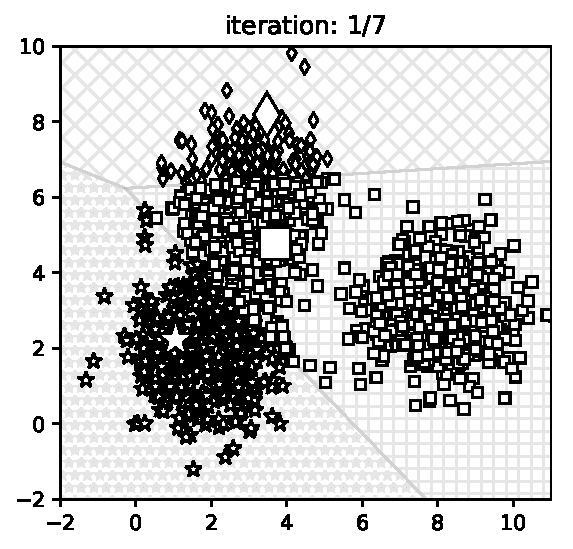
\includegraphics[width=0.99\linewidth]{ebookML_src/src/kmeans/ex_0.pdf}
% \caption{}
% \label{fig:subim1}
\end{subfigure}
\begin{subfigure}{0.325\textwidth}
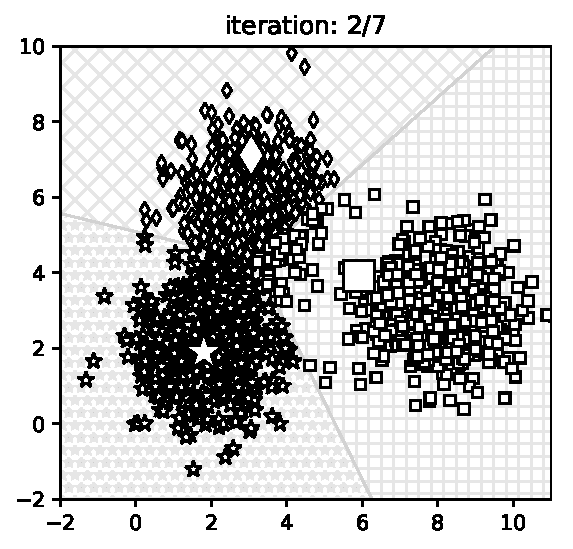
\includegraphics[width=0.99\linewidth]{ebookML_src/src/kmeans/ex_1.pdf}
% \caption{}
% \label{fig:subim2}
\end{subfigure}
\begin{subfigure}{0.325\textwidth}
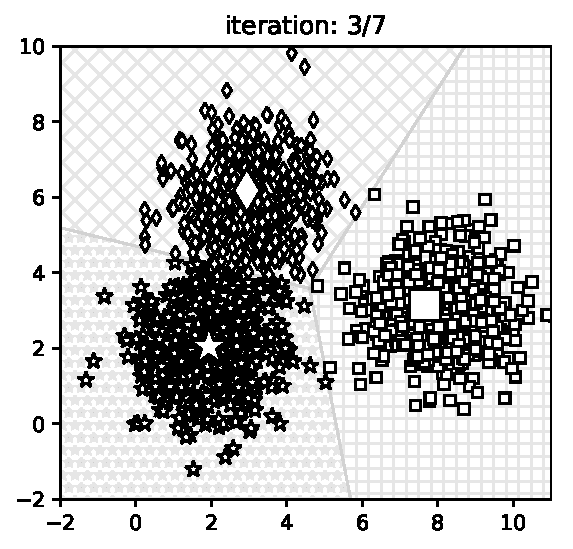
\includegraphics[width=0.99\linewidth]{ebookML_src/src/kmeans/ex_2.pdf}
% \caption{}
% \label{fig:subim2}
\end{subfigure}

\begin{subfigure}{0.325\textwidth}
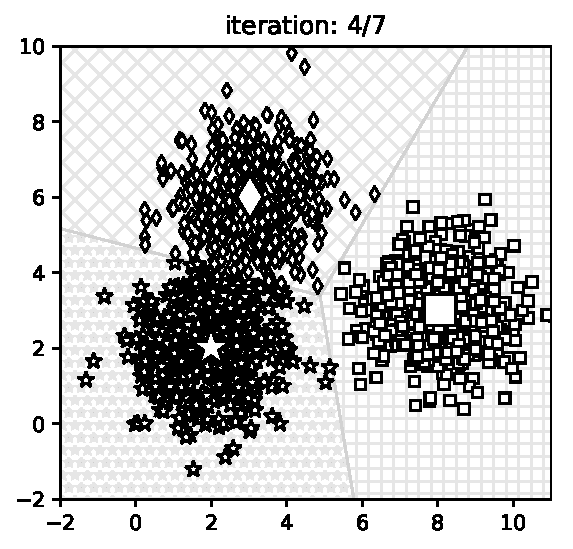
\includegraphics[width=0.99\linewidth]{ebookML_src/src/kmeans/ex_3.pdf}
% \caption{}
% \label{fig:subim1}
\end{subfigure}
\begin{subfigure}{0.325\textwidth}
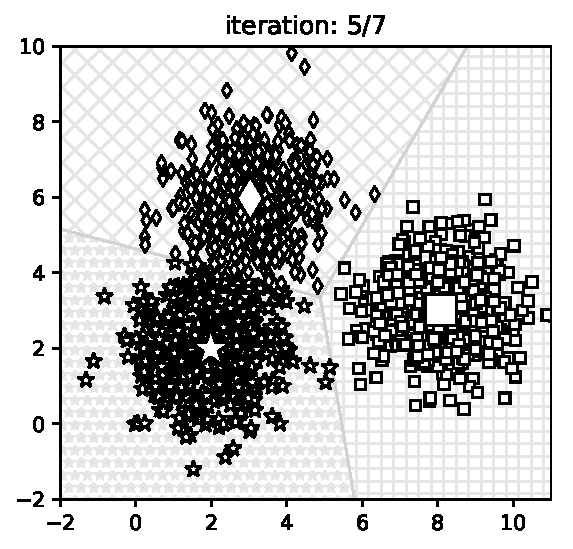
\includegraphics[width=0.99\linewidth]{ebookML_src/src/kmeans/ex_4.pdf}
% \caption{}
% \label{fig:subim2}
\end{subfigure}
\begin{subfigure}{0.325\textwidth}
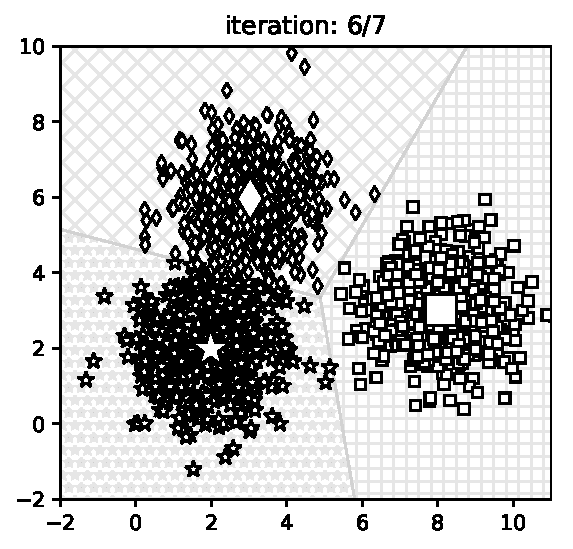
\includegraphics[width=0.99\linewidth]{ebookML_src/src/kmeans/ex_5.pdf}
% \caption{}
% \label{fig:subim2}
\end{subfigure}
\caption{
Thuật toán phân cụm $K$-means qua các vòng lặp.
}
\label{fig:4_example}
\end{figure}


% Các bạn có thể xem thêm các trang web minh họa thuật toán K-means cluster tại:


\subsection{Kết quả tìm được bằng thư viện scikit-learn}

Để kiểm tra thêm, chúng ta hãy so sánh kết quả trên với kết quả thu được bằng
cách sử dụng thư viện
\href{http://scikit-learn.org/stable/modules/generated/sklearn.cluster.KMeans.html}{\pythoninline{scikit-learn}}.

\begin{lstlisting}[language=Python]
from sklearn.cluster import KMeans
model = KMeans(n_clusters=3, random_state=0).fit(X)
print('Centers found by scikit-learn:')
print(model.cluster_centers_)
pred_label = model.predict(X)
kmeans_display(X, pred_label)
\end{lstlisting}
\kq
\begin{lstlisting}
Centroids found by scikit-learn:
[[ 8.0410628   3.02094748]
[ 2.99357611  6.03605255]
[ 1.97634981  2.01123694]]
\end{lstlisting}
Ta nhận thấy rằng các tâm cụm tìm được rất gần với kết quả kỳ vọng.

Tiếp theo, chúng ta cùng xem xét ba ứng dụng đơn giản của phân cụm $K$-means.

% <div class="imgcap">
% <img src ="/assets/kmeans/output_14_1.png" align = "centroid">
% </div>


% Thật may mắn (\textit{cho tôi}), hai thuật toán cho cùng một đáp số! Với cách
% thứ nhất, tôi mong muốn các bạn hiểu rõ được thuật toán K-means clustering làm
% việc như thế nào. Với cách thứ hai, tôi hy vọng các bạn biết áp dụng thư viện
% sẵn có như thế nào.



\section{Phân cụm chữ số viết tay }

\subsection{Bộ cơ sở dữ liệu MNIST }
\index{MNIST}

MNIST~\cite{lecun2010mnist} là bộ cơ sở dữ liệu lớn nhất về chữ số viết tay và
được sử dụng trong hầu hết các thuật toán phân loại hình ảnh. MNIST bao gồm hai
tập con: tập huấn luyện có 60 nghìn mẫu và tập kiểm tra có 10 nghìn mẫu. Tất cả
đều đã được gán nhãn. Hình~\ref{fig:5_mnist} hiển thị 200 mẫu được trích ra từ
MNIST.




Mỗi bức ảnh là một ảnh xám (chỉ có một kênh), có kích thước $28\times28$
điểm ảnh (tức 784 điểm ảnh). Mỗi điểm ảnh mang giá trị là một số tự nhiên từ 0
đến 255. Các điểm ảnh màu đen có giá trị bằng không, các điểm ảnh càng trắng thì có giá trị càng cao. Hình~\ref{fig:5_digit7} là một ví dụ về chữ
số 7 và giá trị các điểm ảnh của nó\footnote{Vì mục đích hiển thị ma trận điểm ảnh ở
bên phải, bức ảnh kích thước $28 \times 28$ ban đầu đã được resize về kích thước
$14 \times 14$.}.

\begin{figure}[t]
% caption on side
\floatbox[{\capbeside\thisfloatsetup{capbesideposition={right,top},capbesidewidth=.2\textwidth}}]{figure}[\FBwidth]
{\caption{
200 mẫu ngẫu nhiên trong bộ cơ sở dữ liệu MNIST.
}
\label{fig:5_mnist}}
{ % figure here
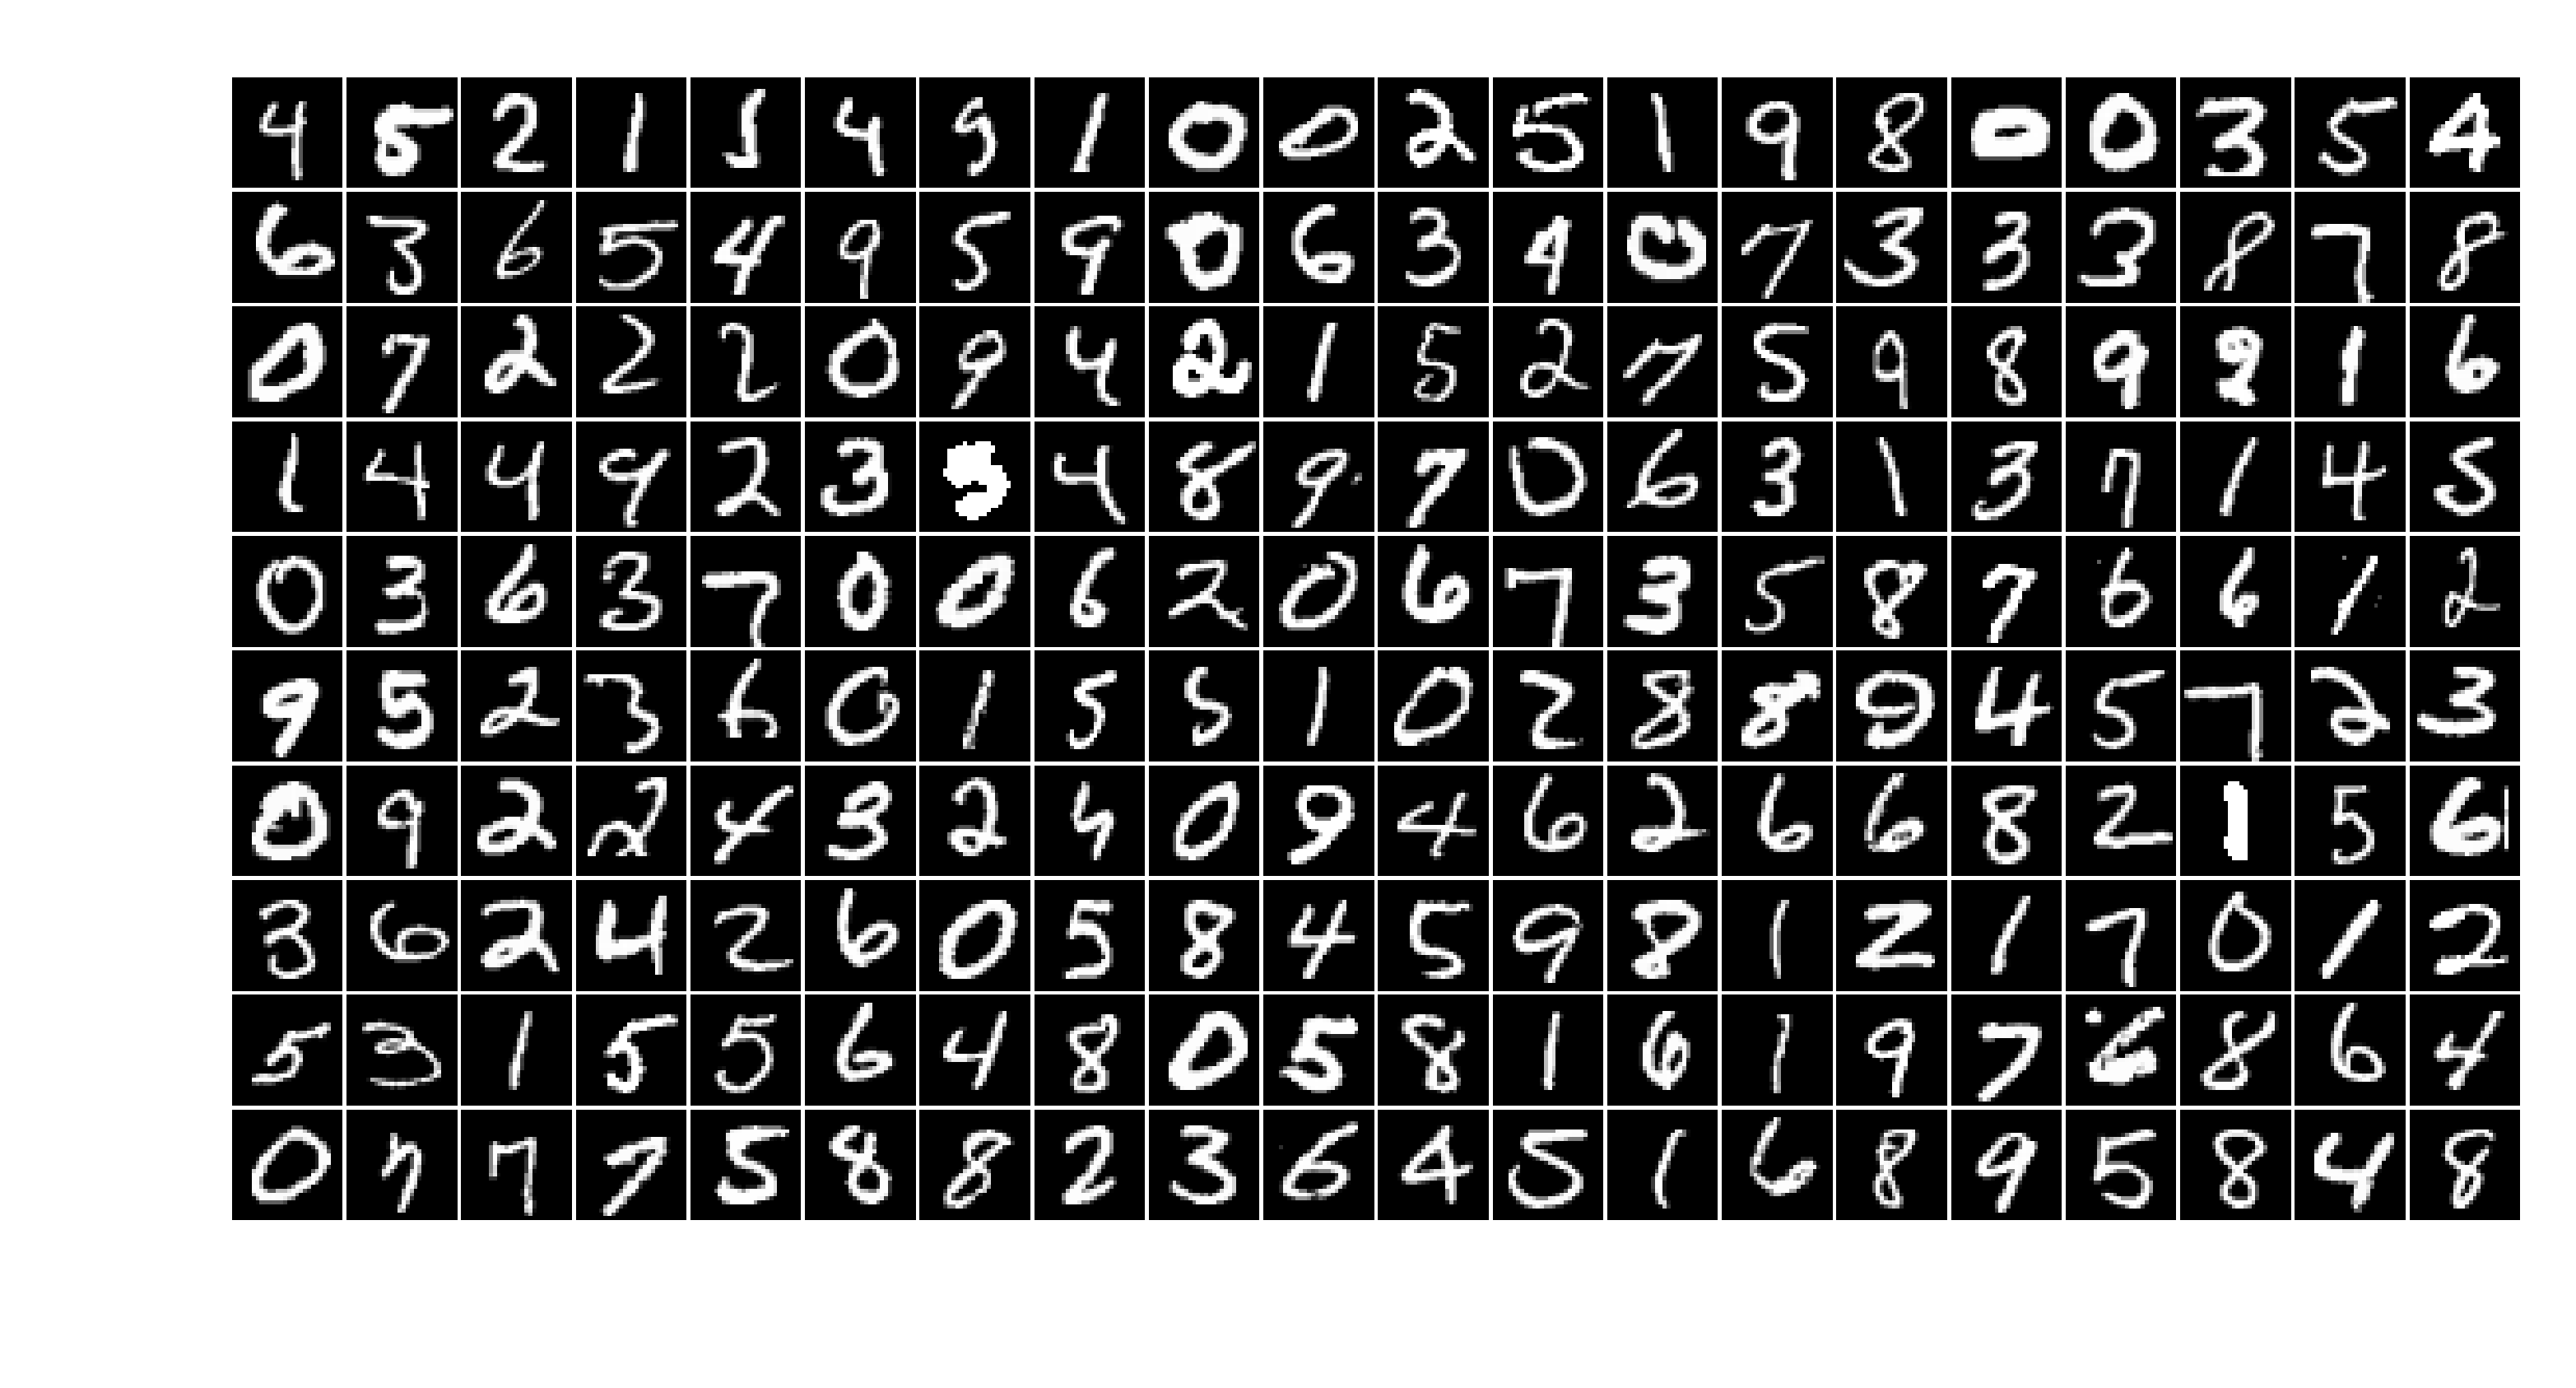
\includegraphics[width=.75\textwidth]{ebookML_src/src/kmeans/mnist_ex.png}
}
\end{figure}
\begin{figure}[t]
% caption on side
\floatbox[{\capbeside\thisfloatsetup{capbesideposition={right,top},capbesidewidth=3.5cm}}]{figure}[\FBwidth]
{\caption{
Ví dụ về chữ số 7 và giá trị các pixel của nó.
}
\label{fig:5_digit7}}
{ % figure here
\includegraphics[width=.75\textwidth]{Chapters/03_SimpleML/4_kmeans/digit_7.png}
}
\end{figure}


\subsection{Bài toán phân cụm giả định}
\textit{\textbf{Bài toán}}: Giả sử ta không biết nhãn của các bức ảnh, hãy phân
các bức ảnh gần giống nhau về một cụm.

Bài toán này có thể được giải quyết bằng phân cụm $K$-means. Mỗi bức ảnh có thể
được coi là một điểm dữ liệu với vector đặc trưng là vector cột 784 chiều.
Vector này nhận được bằng cách chồng các cột của ma trận điểm ảnh lên nhau.

% Trước khi áp dụng thuật toán
% \href{http://machinelearningcoban.com/2017/01/01/kmeans/}{K-means clustering},
% chúng ta cần coi mỗi bức ảnh là một điểm dữ liệu. Và vì mỗi điểm dữ liệu là 1
% vector (hàng hoặc cột) chứ không phải ma trận như số 7 ở trên, chúng ta phải làm
% thêm một bước đơn giản trung gian gọi là \textit{vectorization} (vector hóa).
% Nghĩa là, để có được 1 vector, ta có thể tách các hàng của ma trận pixel ra, sau đó
% đặt chúng cạnh nhau, và chúng ta được một vector hàng rất dài biểu diễn 1 bức
% ảnh chữ số.

% \textbf{Chú ý}: \textit{Cách làm này chỉ là cách đơn giản nhất để mô tả dữ liệu
% ảnh bằng 1 vector. Trên thực tế, người ta áp dụng rất nhiều kỹ thuật khác nhau để
% có thể tạo ra các vector đặc trưng (feature vector) giúp các thuật toán có được
% kết quả tốt hơn.}


\subsection{Làm việc trên Python}
Để tải về MNIST, chúng ta có thể dùng trực tiếp một hàm số trong scikit-learn:

\begin{lstlisting}[language=Python]
from __future__ import print_function
import numpy as np
from sklearn.datasets import fetch_mldata

data_dir = '../../data' # path to your data folder
mnist = fetch_mldata('MNIST original', data_home=data_dir)
print("Shape of minst data:", mnist.data.shape)
\end{lstlisting}
\kq
\begin{lstlisting}[language=Python]
Shape of minst data: (70000, 784)
\end{lstlisting}
\pythoninline{shape} của ma trận dữ liệu \pythoninline{mnist.data} là
\pythoninline{(70000, 784)} tức có 70000 mẫu, mỗi mẫu có kích thước 784. Chú ý
rằng trong scikit-learn, mỗi điểm dữ liệu thường được lưu dưới dạng một vector
hàng. Tiếp theo, chúng ta lấy ra ngẫu nhiên 10000 mẫu và thực hiện phân cụm $K$-means
trên tập con này:
% \newpage
\begin{lstlisting}[language=Python]
from sklearn.cluster import KMeans
from sklearn.neighbors import NearestNeighbors
K = 10 # number of clusters
N = 10000
X = mnist.data[np.random.choice(mnist.data.shape[0], N)]
kmeans = KMeans(n_clusters=K).fit(X)
pred_label = kmeans.predict(X)
\end{lstlisting}





Sau khi thực hiện đoạn code trên, các tâm cụm được lưu trong biến
\pythoninline{kmeans.cluster_centers_}, nhãn của mỗi điểm dữ liệu được lưu
trong biến \pythoninline{pred_label}. Hình~\ref{fig:5_random} hiển thị các tâm
cụm tìm được và 20 mẫu ngẫu nhiên được phân vào cụm tương ứng. Mỗi hàng tương
ứng với một cụm, cột đầu tiên bên trái là các tâm cụm tìm được. Ta thấy rằng các
tâm cụm đều giống với một chữ số hoặc là kết hợp của hai/ba chữ số nào đó. Ví
dụ, tâm cụm ở hàng thứ tư là sự kết hợp của các chữ số 4, 7, 9; ở hàng thứ bảy là kết
hợp của các chữ số 7, 8 và 9.





Nhận thấy rằng các bức ảnh lấy ra ngẫu nhiên từ mỗi cụm không thực sự giống
nhau. Lý do có thể vì những bức ảnh này ở xa các tâm cụm mặc dù tâm cụm đó đã là
gần nhất. Như vậy phân cụm $K$-means làm việc chưa thực sự tốt trong trường hợp
này. Tuy nhiên, chúng ta vẫn có thể khai thác một số thông tin hữu ích sau khi
thực hiện thuật toán. Thay vì chọn ngẫu nhiên các bức ảnh trong mỗi cụm, ta chọn
20 bức ảnh gần tâm của mỗi cụm nhất, vì càng gần tâm thì độ tin cậy càng cao.
Quan sát Hình~\ref{fig:5_knn}, có thể thấy dữ liệu trong mỗi hàng khá giống nhau
và giống với tâm cụm ở cột đầu tiên bên trái. Từ đây có thể rút ra một vài quan
sát thú vị:

\begin{enumerate}
\item Có hai kiểu viết chữ số 1 -- thẳng và chéo. Phân cụm $K$-means
nghĩ rằng đó là hai chữ số khác nhau. Điều này là dễ hiểu vì phân cụm $K$-means
là một thuật toán học không giám sát. Nếu có sự can thiệp của
con người, chúng có thể được nhóm lại thành một.


\item Ở hàng thứ chín, chữ số 4 và 9 được phân vào cùng một cụm. Sự
thật là hai chữ số này khá giống nhau. Điều tương tự xảy ra đối với
hàng thứ bảy với các chữ số 7, 8, 9. Phân cụm $K$-means có thể được áp dụng để tiếp tục phân nhỏ các cụm đó.

\end{enumerate}

\begin{figure}[t]
% caption on side
\floatbox[{\capbeside\thisfloatsetup{capbesideposition={right,top},capbesidewidth=4cm}}]{figure}[\FBwidth]
{\caption{
Các tâm cụm (cột đầu) và 20 điểm {ngẫu nhiên} trong mỗi cụm. Các chữ số trên mỗi hàng thuộc vào cùng một cụm.
}
\label{fig:5_random}}
{ % figure here
% \includegraphics[width=.65\textwidth]{Chapters/03_SimpleML/4_kmeans/kmeans_random.png}
\includegraphics[width=.65\textwidth]{Chapters/03_SimpleML/4_kmeans/kmeans_random_gray.png}
}
\end{figure}

\begin{figure}[t]
% caption on side
\floatbox[{\capbeside\thisfloatsetup{capbesideposition={right,top},capbesidewidth=4cm}}]{figure}[\FBwidth]
{\caption{
Tâm và 20 điểm gần tâm nhất của mỗi cụm.
}
\label{fig:5_knn}}
{ % figure here
% \includegraphics[width=.65\textwidth]{Chapters/03_SimpleML/4_kmeans/kmeans_knn.png}
\includegraphics[width=.65\textwidth]{Chapters/03_SimpleML/4_kmeans/kmeans_knn_gray.png}
}
\end{figure}

\index{phân cụm theo tầng -- hierarchical clustering}
\index{hierarchical clustering -- phân cụm theo tầng}
Một kỹ thuật phân cụm thường được sử dụng là \textit{phân cụm theo
tầng} (\textit{hierarchical clustering}~\cite{blei2008hierarchical}). Có hai
loại phân cụm theo tầng:

\begin{itemize}
\item \textit{Agglomerative} tức ``đi từ dưới lên''. Ban đầu ta chọn $K$ là một
số lớn gần bằng số điểm dữ liệu. Sau khi thực hiện phân cụm $K$-means lần
đầu, các cụm gần nhau được ghép lại thành một cụm. Khoảng cách giữa các cụm có thể được xác định bằng khoảng cách giữa các tâm cụm. Sau bước này, ta thu được một
số lượng cụm nhỏ hơn. Tiếp tục phân cụm $K$-means với điểm khởi tạo
là tâm của cụm lớn vừa thu được. Lặp lại quá trình này đến khi nhận
được kết quả chấp nhận được.

\item \textit{Divisive} tức ``đi từ trên xuống''. Ban đầu, thực hiện phân
cụm $K$-means với $K$ nhỏ để được các cụm lớn. Sau đó tiếp tục áp dụng phân cụm $K$-means vào mỗi cụm lớn đến khi kết quả chấp nhận được.

\end{itemize}

% \newpage
\section{Tách vật thể trong ảnh}


% \subsection{Đặt vấn đề}
Phân cụm $K$-means cũng được áp dụng vào bài toán \textit{tách vật thể trong ảnh} (\textit{object segmentation}). Cho bức ảnh như trong Hình~\ref{fig:5_girl}, hãy xây dựng một thuật toán tự động nhận diện và tách rời vùng khuôn mặt.

% ******************************************************************************
\begin{figure}[t]
% caption on side
\floatbox[{\capbeside\thisfloatsetup{capbesideposition={right,top},capbesidewidth=6cm}}]{figure}[\FBwidth]
{\caption{
\textit{Ảnh:Trọng Vũ} (\url{https://goo.gl/9D8aXW}, xem ảnh màu trong Hình~\ref{fig:5_girl_c}) .
}
\label{fig:5_girl}}
{ % figure here
\includegraphics[width=.5\textwidth]{Chapters/03_SimpleML/4_kmeans/girl3_gray.jpg}
% \includegraphics[width=.5\textwidth]{Chapters/03_SimpleML/4_kmeans/girl3.jpg}
}
\end{figure}
% ******************************************************************************


% <div class="imgcap">
% <img src ="/assets/kmeans/girl3.jpg" align = "centroid">
% <div class="thecap">Credit ảnh: <a href = "https://www.facebook.com/photo.php?fbid=1219980151402370&set=a.113129725420757.13101.100001711890571&type=3&theater"> Trọng Vũ</a>
% </div>
% </div>


% \subsection{Lên ý tưởng  }
% (\textit{Lại giả sử rằng chúng ta chưa biết gì khác ngoài K-means clustering,
% các bạn hãy dừng vài giây để nghĩ xem chúng ta có thể xử lý thế nào. Gợi ý: Có
% ba màu chủ đạo trong bức ảnh.})

% Ok, có ba màu, ba clusters!

Bức ảnh có ba màu chủ đạo: hồng ở khăn và môi; đen ở mắt, tóc, và hậu cảnh; màu
da ở vùng còn lại của khuôn mặt. Ảnh này khá rõ nét và các vùng được phân biệt
rõ ràng bởi màu sắc nên chúng ta có thể áp dụng thuật toán phân cụm $K$-means.
Thuật toán này sẽ phân các điểm ảnh thành ba cụm, cụm chứa phần khuôn mặt có thể được chọn tự động hoặc bằng tay.

Đây là một bức ảnh màu, mỗi điểm ảnh được biểu diễn bởi ba giá trị tương ứng với
màu đỏ, lục, và lam (RGB). Nếu coi mỗi điểm ảnh là một điểm dữ liệu được mô tả
bởi một vector ba chiều chứa các giá trị này, sau đó áp dụng phân cụm $K$-means,
chúng ta có thể đạt được kết quả như mong muốn.



\subsection{Làm việc trên Python}

{Khai báo thư viện và hiển thị bức ảnh:}

\begin{lstlisting}[language=Python]
import matplotlib.image as mpimg
import matplotlib.pyplot as plt
import numpy as np
from sklearn.cluster import KMeans
img = mpimg.imread('girl3.jpg')
plt.imshow(img)
imgplot = plt.imshow(img)
plt.axis('off')
plt.show()
\end{lstlisting}


{Biến đổi bức ảnh thành một ma trận mà mỗi hàng là ba giá trị màu của một điểm ảnh:}
\begin{lstlisting}[language=Python]
X = img.reshape((img.shape[0]*img.shape[1], img.shape[2]))
\end{lstlisting}

Phần còn lại của mã nguồn có thể được tìm thấy tại \url{https://goo.gl/Tn6Gec}.


% <div class="imgcap">
% <img src ="/assets/kmeans/girl_seg.png" align = "centroid">
% </div>

\begin{figure}[t]
% caption on side
\floatbox[{\capbeside\thisfloatsetup{capbesideposition={right,top},capbesidewidth=6cm}}]{figure}[\FBwidth]
{\caption{
Kết quả nhận được sau khi thực hiện phân cụm $K$-means.
Có ba cụm tương ứng với ba màu đỏ, hồng, đen (xem ảnh màu trong Hình~\ref{fig:5_girl_seg_c}).
}
\label{fig:5_girl_seg}}
{ % figure here
\includegraphics[width=.5\textwidth]{Chapters/03_SimpleML/4_kmeans/girl_seg_gray.png}
}
\end{figure}

Sau khi tìm được các cụm, giá trị của mỗi pixel được thay bằng giá trị của
tâm tương ứng. Kết quả được minh hoạ trên Hình~\ref{fig:5_girl_seg}. Ba màu
đỏ, đen, và màu da (xem ảnh màu trong Hình~\ref{fig:5_girl_seg_c}) đã được phân
nhóm khá thành công. Khuôn mặt có thể được tách ra từ phần có màu da và vùng
bên trong nó. Như vậy, phân cụm $K$-means tạo ra một kết quả chấp nhận được
cho bài toán này.


\section{Nén ảnh}

Trước hết, xét đoạn code dưới đây:

\begin{lstlisting}[language=Python]
for K in [5, 10, 15, 20]:
    kmeans = KMeans(n_clusters=K).fit(X)
    label = kmeans.predict(X)

img4 = np.zeros_like(X)
# replace each pixel by its centroid
for k in range(K):
    img4[label == k] = kmeans.cluster_centroids_[k]
# reshape and display output image
img5 = img4.reshape((img.shape[0], img.shape[1], img.shape[2]))
plt.imshow(img5, interpolation='nearest')
plt.axis('off')
plt.show()
\end{lstlisting}

Nhận thấy rằng mỗi điểm ảnh có thể nhận một trong số $256^3 \approx $ 16 triệu
màu. Đây là một số rất lớn (tương đương với 24 bit cho một điểm ảnh). Phân cụm
$K$-means có thể được áp dụng để nén ảnh với số bit ít hơn. Phép nén ảnh này làm
mất dữ liệu nhưng kết quả vẫn chấp nhận được. Quay trở lại bài toán tách vật thể
trong mục trước, nếu thay mỗi điểm ảnh bằng tâm cụm tương ứng, ta thu được một
bức ảnh nén. Tuy nhiên, chất lượng bức ảnh rõ ràng đã giảm đi nhiều. Trong đoạn
code trên đây, ta đã làm một thí nghiệm nhỏ với số lượng cụm tăng lên 5, 10, 15,
20. Sau khi tìm được tâm cho mỗi cụm, giá trị của một điểm ảnh được thay bằng
giá trị của tâm tương ứng. Kết quả được hiển thị trên Hình~\ref{fig:5_res}. Có
thể thấy rằng khi số lượng cụm tăng lên, chất lượng bức ảnh đã được cải thiện.
Để nén bức ảnh này, ta chỉ cần lưu $K$ tâm cụm tìm được và nhãn của mỗi điểm
ảnh.



\begin{figure}[t]
\centering
\includegraphics[width = \textwidth]{Chapters/03_SimpleML/4_kmeans/girl_all_gray.png}
\caption[]{Chất lượng nén ảnh với số lượng cluster khác nhau (xem ảnh màu trong Hình~\ref{fig:5_res_c}).}
\label{fig:5_res}
\end{figure}


\section{Thảo luận}
\subsection{Hạn chế của phân cụm $K$-means}


% \subsection{Hạn chế}
\index{phương pháp elbow}
% Có một vài hạn chế của thuật toán phân cụm $K$-means:
\begin{itemize}
\item \textit{Số cụm $K$ cần được xác định trước.}
Trong trường hợp, chúng ta không biết trước giá trị này. Bạn đọc có thể tham khảo \textit{phương pháp elbow} giúp xác định giá trị $K$ này (\url{https://goo.gl/euYhpK}).
% ******************************************************************************
\begin{figure}[t]
\begin{subfigure}{0.325\textwidth}
\includegraphics[width=0.99\linewidth]{ebookML_src/src/kmeans/dif_res10.pdf}
\caption{}
\label{fig:4_dif_resa}
\end{subfigure}
\begin{subfigure}{0.325\textwidth}
\includegraphics[width=0.99\linewidth]{ebookML_src/src/kmeans/dif_res31.pdf}
\caption{}
\label{fig:4_dif_resb}
\end{subfigure}
\begin{subfigure}{0.325\textwidth}
\includegraphics[width=0.99\linewidth]{ebookML_src/src/kmeans/dif_res27.pdf}
\caption{}
\label{fig:4_dif_resc}
\end{subfigure}
\caption{
Các giá trị khởi tạo ban đầu khác nhau dẫn đến các nghiệm khác nhau.
}
\label{fig:4_dif_res}
\end{figure}
% ******************************************************************************
\item \textit{Nghiệm cuối cùng phụ thuộc vào các tâm cụm được khởi tạo ban
đầu.}
Thuật toán phân cụm $K$-means không đảm bảo tìm được nghiệm tối ưu toàn cục, nghiệm cuối cùng phụ thuộc vào các tâm cụm được khởi tạo ban đầu.
Hình~\ref{fig:4_dif_res} thể hiện các kết quả khác nhau khi các tâm cụm
được khởi tạo khác nhau. Ta cũng thấy rằng trường hợp (a) và (b) cho kết quả
tốt, trong khi kết quả thu được ở trường hợp (c) không thực sự tốt. Một điểm
nữa có thể rút ra là số lượng vòng lặp tới khi thuật toán hội tụ cũng khác
nhau. Trường hợp (a) và (b) cùng cho kết quả tốt nhưng (b) chạy trong thời
gian gần gấp đôi. Một kỹ thuật giúp hạn chế nghiệm xấu như trường hợp (c) là
chạy thuật toán phân cụm $K$-means nhiều lần với các tâm cụm được khởi tạo
khác nhau và chọn ra lần chạy cho giá trị hàm mất mát thấp nhất\footnote{\textit{KMeans -- scikit-learn} (\url{https://goo.gl/5KavVn}).}. Ngoài ra, có một vài thuật toán giúp chọn các tâm cụm ban đầu~\cite{khan2004cluster},
Kmeans++~\cite{arthur2007k,bahmani2012scalable}.

\item \textit{Các cụm cần có số lượng điểm gần bằng nhau}.
Hình~\ref{fig:4_disa} minh hoạ kết quả khi các cụm có số điểm
chênh lệch. Trong trường hợp này, nhiều điểm lẽ ra thuộc cụm hình vuông đã bị phân nhầm vào cụm hình sao.

\index{Gaussion mixture model}
\item \textit{Các cụm cần có dạng hình tròn (cầu)}.
Khi các cụm vẫn tuân theo phân phối chuẩn nhưng ma trận hiệp phương sai
không tỉ lệ với ma trận đơn vị, các cụm sẽ không có dạng tròn
(hoặc cầu trong không gian nhiều chiều). Khi đó, phân cụm $K$-means không hoạt động hiệu quả. Lý do chính là vì phân cụm $K$-means quyết định
nhãn của một điểm dữ liệu dựa trên khoảng cách Euclid của nó tới các
tâm. Trong trường hợp này, \textit{Gaussian mixture models} (GMM)~\cite{reynolds2015gaussian} có thể cho kết quả tốt hơn\footnote{Đọc thêm:
\textit{Gaussian mixture models -- Wikipedia} (\url{https://goo.gl/GzdauR}).}. Trong GMM, mỗi cụm được giả sử tuân theo một phân phối chuẩn với ma trận hiệp phương sai không nhất thiết tỉ lệ với ma trận đơn vị. Ngoài các tâm cụm, các ma trận hiệp phương sai cũng là các biến cần tối ưu trong GMM.


\index{phân cụm spectral -- spectral clustering}
\index{spectral clustering -- phân cụm spectral}
\item \textit{Khi một cụm nằm trong cụm khác}.
Hình~\ref{fig:4_face} là một ví dụ kinh điển về việc phân cụm $K$-means
không làm việc. Một cách tự nhiên, chúng ta sẽ phân dữ liệu ra thành bốn
cụm: mắt trái, mắt phải, miệng, xung quanh mặt. Nhưng vì mắt và miệng nằm
trong khuôn mặt nên phân cụm $K$-means cho kết quả không chính xác. Với dữ
liệu như trong ví dụ này, \textit{phân cụm
spectral}~\cite{von2007tutorial,ng2002spectral} sẽ cho kết quả tốt hơn. Phân
cụm spectral cũng coi các điểm gần nhau tạo thành một cụm, nhưng không giả
sử về một tâm chung cho cả cụm. Phân cụm spectral được thực hiện dựa trên
một đồ thị vô hướng với đỉnh là các điểm dữ liệu và cạnh được nối giữa các
điểm gần nhau, mỗi cạnh được đánh trọng số là một hàm của khoảng cách giữa
hai điểm.


\end{itemize}


% ******************************************************************************
\begin{figure}[ht]
\begin{subfigure}{0.49\textwidth}

\includegraphics[width=0.8\linewidth]{ebookML_src/src/kmeans/skew_10.pdf}
\caption{}
\label{fig:4_disa}
\end{subfigure}
\begin{subfigure}{0.49\textwidth}

\includegraphics[width=0.8\linewidth]{ebookML_src/src/kmeans/notround_10.pdf}
\caption{}
\label{fig:4_disb}
\end{subfigure}
\caption{
Phân cụm $K$-means hoạt động không thực sự tốt trong trường hợp các
cụm có số lượng phần tử chênh lệch hoặc các cụm không có dạng
hình tròn.
}
\label{fig:4_dis}
\end{figure}
% ******************************************************************************



\begin{figure}[ht]
% caption on side
\floatbox[{\capbeside\thisfloatsetup{capbesideposition={right,top},capbesidewidth=6.5cm}}]{figure}[\FBwidth]
{\caption{
Một ví dụ về việc phân cụm $K$-means không hoạt động hiệu quả.
}
\label{fig:4_face}}
{ % figure here
% \includegraphics[width=.55\textwidth]{Chapters/03_SimpleML/4_kmeans/smile_face.png}
\includegraphics[width=.3\textwidth]{Chapters/03_SimpleML/4_kmeans/smile_face_gray.png}
}
\end{figure}

\subsection{Các ứng dụng khác của phân cụm $K$-means}
Mặc dù có những hạn chế, phân cụm $K$-means vẫn cực kỳ quan trọng trong machine
learning và là nền tảng cho nhiều thuật toán phức tạp khác. Dưới đây là một vài ứng dụng khác của phân cụm $K$-means.
% \begin{enumerate}
% \item Với một thuật toán K-means clustering đơn giản, chúng ta đã có thể áp
% dụng nó vào các bài toán thực tế. Mặc dù kết quả chưa thực sự như ý, chúng ta
% vẫn thấy được tiềm năng của thuật toán đơn giản này.

Cách thay một điểm dữ liệu bằng tâm cụm tương ứng là một trong số các
kỹ thuật có tên chung là \textit{vector quantization  --
VQ}~\cite{arya1993algorithms}). Không chỉ được áp dụng trong nén dữ liệu, VQ
còn được kết hợp với Bag-of-Words\cite{lazebnik2006beyond} áp dụng rộng rãi
trong các thuật toán xây dựng vector đặc trưng.


Ngoài ra, VQ cũng được áp dụng vào các bài toán tìm kiếm trong cơ sở dữ liệu
lớn. Khi số điểm dữ liệu là rất lớn, việc tìm kiếm trở nên cực kỳ quan
trọng. Khó khăn chính của việc này là làm thế nào có thể tìm kiếm một cách
nhanh chóng trong lượng dữ liệu khổng lồ đó. Ý tưởng cơ bản là sử dụng các
thuật toán phân cụm để phân các điểm dữ liệu thành nhiều cụm nhỏ. Để tìm các
điểm gần nhất của một điểm \textit{truy vấn}, ta có thể tính khoảng cách
giữa điểm này và các tâm cụm thay vì toàn bộ các
điểm trong cơ sở dữ liệu. Bạn đọc có thể đọc thêm các bài báo nổi tiếng gần
đây về vấn đề này: Product Quantization~\cite{jegou2011product}, Cartesian
k-means~\cite{norouzi2013cartesian,johnson2017billion}, Composite
Quantization~\cite{zhang2014composite}, Additive
Quantization~\cite{babenko2014additive}.


% \end{enumerate}
Mã nguồn cho chương này có thể được tìm thấy tại \url{https://goo.gl/QgW5f2}.



\subsection{Đọc thêm}

\begin{enumerate}
\item \textit{Clustering documents using k-means -- scikit-learn} (\url{https://goo.gl/y4xsy2}).

\item \textit{Voronoi Diagram -- Wikipedia} (\url{https://goo.gl/v8WQEv}).

\item \textit{Cluster centroid initialization algorithm for K-means clustering} (\url{https://goo.gl/hBdody}).

\item \textit{Visualizing K-Means Clustering} (\url{https://goo.gl/ULbpUM}).

\item \textit{Visualizing K-Means Clustering -- Standford} (\url{https://goo.gl/idzR2i}).

\end{enumerate}


%!TEX root = ../../book_ML.tex
\addtocontents{toc}{\protect\newpage}
\chapter{Bộ phân loại naive Bayes}
\label{cha:nbc}
\index{bộ phân loại naive Bayes -- naive Bayes classifier}
\index{naive Bayes classifier -- bộ phân loại naive Bayes}
\index{NBC}

\section{Bộ phân loại naive Bayes}

Xét các bài toán phân loại với $C$ nhãn khác nhau. Thay vì tìm ra chính
xác nhãn của mỗi điểm dữ liệu $\bx \in \R^d$, ta có thể đi tìm xác suất để kết quả rơi vào mỗi nhãn:
\begin{math}
\label{eqn:32_1}
p(y = c |\mathbf{x})
\end{math},
hoặc viết gọn thành $p(c|\mathbf{x})$. Biểu thức này được hiểu là xác suất để
đầu ra là nhãn $c$ biết rằng đầu vào là vector $\mathbf{x}$. Nếu tính được biểu thức này, ta có thể giúp xác định nhãn của mỗi điểm dữ liệu bằng cách chọn ra
nhãn có xác suất rơi vào cao nhất:
\begin{equation}
\label{eqn:32_2}
c = \argmax_{c \in \{1, \dots, C\}} p(c | \mathbf{x})
\end{equation}
Nhìn chung, khó có cách tính trực tiếp $p(c|\bx)$. Thay vào đó,
quy tắc Bayes thường được sử dụng:
\begin{align}
c =  \argmax_c p(c | \mathbf{x}) =
\argmax_c \frac{p(\mathbf{x} | c) p(c)}{p(\mathbf{x})}
=  \argmax_c p(\mathbf{x} | c) p(c)
\end{align}
Dấu bằng thứ hai xảy ra theo quy tắc Bayes, dấu bằng thứ ba xảy ra vì $p(\bx)$ ở
mẫu số không phụ thuộc vào $c$. Tiếp tục quan sát, $p(c)$ có thể được hiểu là
xác suất để một điểm \textit{bất kỳ} rơi vào nhãn $c$. Nếu tập huấn luyện lớn,
$p(c)$ có thể được xác định bằng phương pháp ước lượng hợp lý cực đại (MLE) -- là
tỉ lệ giữa số điểm thuộc nhãn $c$ và số điểm trong tập huấn luyện. Nếu tập huấn
luyện nhỏ, giá trị này có thể được xác định bằng phương pháp ước lượng hậu
nghiệm cực đại (MAP).

Thành phần còn lại $p(\mathbf{x} | c)$ là phân phối của các điểm dữ liệu trong
nhãn $c$. Thành phần này thường rất khó tính toán vì $\mathbf{x}$ là một biến
ngẫu nhiên nhiều chiều. Để có thể ước lượng được phân phối đó, tập huấn luyện
phải rất lớn. Nhằm đơn giản hoá việc tính toán, người ta thường giả sử
rằng các thành phần của biến ngẫu nhiên $\mathbf{x}$ độc lập với nhau khi đã
biết $c$:
\begin{equation}
\label{eqn:32_6}
p(\mathbf{x} | c) = p(x_1, x_2, \dots, x_d | c) =  \prod_{i = 1}^d p(x_i | c)
\end{equation}
Giả thiết các chiều của dữ liệu độc lập với nhau là quá chặt và trên thực tế, ít
khi tìm được dữ liệu mà các thành phần hoàn toàn độc lập với nhau. Tuy nhiên,
giả thiết \textit{ngây thơ} (\textit{naive}) này đôi khi mang lại những kết quả
tốt bất ngờ. Giả thiết về sự độc lập của các chiều dữ liệu này được gọi là
\textit{naive Bayes}. Một phương pháp xác định nhãn của dữ liệu dựa trên giả
thiết này có tên là \textit{phân loại naive Bayes (NBC)}.

Nhờ giả thiết độc lập, NBC có tốc độ huấn luyện và
kiểm tra rất nhanh. Việc này rất quan trọng trong các bài toán với dữ liệu lớn.

Ở bước huấn luyện, các phân phối $p(c)$ và $p(x_i | c), i = 1, \dots, d$ được xác định dựa vào dữ liệu huấn luyện. Việc xác định các giá trị này có thể được thực hiện bằng MLE hoặc MAP.

Ở bước kiểm tra, nhãn của một điểm dữ liệu mới $\mathbf{x}$ được xác đinh bởi
\begin{equation}
\label{eqn:32_7}
c = \argmax_{c \in \{1, \dots, C\}} p(c) \prod_{i=1}^d p(x_i | c).
\end{equation}
Khi $d$ lớn và các xác suất nhỏ, biểu thức ở vế phải của~\eqref{eqn:32_7} là một
số rất nhỏ, khi tính toán có thể gặp sai số. Để giải quyết việc
này,~\eqref{eqn:32_7} thường được viết lại dưới dạng tương đương bằng cách lấy
$\log$ của vế phải:
\begin{equation}
\label{eqn:32_7_1}
c = \argmax_{c \in \{1, \dots, C\}} \left(\log(p(c)) + \sum_{i=1}^d \log(p(x_i
| c))\right).
\end{equation}
Việc này không ảnh hưởng tới kết quả vì $\log$ là một hàm đồng biến trên tập các số dương.

Sự đơn giản của NBC mang lại hiệu quả đặc biệt trong các bài toán phân loại văn
bản, ví dụ bài toán lọc tin nhắn hoặc email rác. Trong phần sau của
chương này, chúng ta cùng xây dựng một bộ lọc email rác tiếng Anh đơn giản.
Cả quá trình huấn luyện và kiểm tra của NBC đều cực kỳ nhanh so với các phương
pháp phân loại phức tạp khác. Việc giả sử các thành phần trong dữ liệu là độc
lập với nhau khiến cho việc tính toán mỗi phân phối $p(\mathbf{x}_i|c)$ trở nên đơn giản.

% Mỗi giá trị $p(c), c = 1, 2, \dots, C$ có thể được xác định như là tần suất xuất
% hiện của class $c$ trong training data.

Việc tính toán $p(\mathbf{x}_i | c) $ phụ thuộc vào loại dữ liệu. Có ba loại
phân bố xác suất phổ biến là \textit{Gaussian naive Bayes},
\textit{multinomial naive Bayes}, và \textit{Bernoulli Naive}. Chúng ta cùng xem xét  từng loại.





\section{Các phân phối thường dùng trong NBC}

% \textit{Mục này chủ yếu được dịch từ \href{http://scikit-learn.org/dev/modules/naive_bayes.html#naive-bayes}{tài liệu của thư viện sklearn}.}

\subsection{Gaussian naive Bayes }
\index{Gaussian naive Bayes}
Mô hình này được sử dụng chủ yếu trong loại dữ liệu mà các thành phần là các
biến liên tục. Với mỗi chiều dữ liệu $i$ và một nhãn $c$, $x_i$ tuân theo một
phân phối chuẩn có kỳ vọng $\mu_{ci}$ và phương sai $\sigma_{ci}^2$:
\begin{equation}
\label{eqn:32_8}
p(x_i|c) = p(x_i | \mu_{ci}, \sigma_{ci}^2) =  \frac{1}{\sqrt{2\pi \sigma_{ci}^2}} \exp\left(- \frac{(x_i - \mu_{ci})^2}{2 \sigma_{ci}^2}\right)
\end{equation}
Trong đó, bộ tham số $\theta = \{\mu_{ci}, \sigma_{ci}^2\}$ được xác định bằng
MLE\footnote{Xem ví dụ trang~\pageref{sssec:gassian_mle}.} dựa trên các điểm trong tập huấn luyện thuộc nhãn $c$.
% % \begin{equation}
% % \label{eqn:32_9}
% % (\mu_{ci}, \sigma_{ci}^2) = \argmax_{(\mu_{ci}, \sigma_{ci}^2)} \prod_{n = 1}^N p(x_i^{(n)} \| \mu_{ci}, \sigma_{ci}^2)
% % \end{equation}
% % ở đây $\$
% \textit{Đây là cách tính của thư viện sklearn. Chúng ta cũng có thể đánh giá các tham số bằng MAP nếu biết trước priors của $\mu_{ci}$ và $\sigma^2_{ci}$}


\subsection{Multinomial naive Bayes }
\index{multinomial naive Bayes}

Mô hình này chủ yếu được sử dụng trong bài toán phân loại văn bản mà vector đặc
trưng được xây dựng dựa trên ý tưởng bag of words (BoW). Lúc này, mỗi văn bản
được biểu diễn bởi một vector có độ dài $d$ là số từ trong từ điển. Giá trị của
thành phần thứ $i$ trong mỗi vector là số lần từ thứ $i$ xuất hiện trong văn bản
đó. Khi đó, $p(x_i |c) $ tỉ lệ với tần suất từ thứ $i$ (hay đặc trưng thứ $i$
trong trường hợp tổng quát) xuất hiện trong các văn bản có nhãn $c$. Giá trị này
có thể được tính bởi
\begin{equation}
\label{eqn:32_10}
\lambda_{ci} = p(x_i | c) = \frac{N_{ci}}{N_c}.
\end{equation}
Trong đó:
\begin{itemize}
\item $N_{ci}$ là tổng số lần từ thứ $i$ xuất hiện trong các văn bản của
nhãn $c$. Nó chính là tổng tất cả thành phần thứ $i$ của các
vector đặc trưng ứng với nhãn $c$.

\item $N_c$ là tổng số từ, kể cả lặp, xuất hiện trong nhãn $c$. Nói cách
khác, $N_c$ là tổng độ dài của tất cả các văn bản thuộc nhãn $c$. Có
thể suy ra rằng $N_c = \sum_{i = 1}^d N_{ci}$, từ đó $\sum_{i=1}^d
\lambda_{ci} = 1$.
\end{itemize}

\index{làm mềm Laplace -- Laplace smoothing}
\index{Laplace smoothing -- làm mềm Laplace}
Cách tính này có một hạn chế là nếu có một từ mới chưa bao giờ xuất hiện trong
nhãn $c$ thì biểu thức~\eqref{eqn:32_10} sẽ bằng không, dẫn đến vế phải
của~\eqref{eqn:32_7} bằng không bất kể các giá trị còn lại lớn thế nào (xem
thêm ví dụ ở mục sau). Để giải quyết việc này, một kỹ thuật được gọi là
\textit{làm mềm Laplace} (Laplace smoothing) được áp dụng:
\begin{equation}
\label{eqn:32_11}
\hat{\lambda}_{ci} = \frac{N_{ci} + \alpha}{N_{c} + d\alpha}
\end{equation}
với $\alpha$ là một số dương, thường bằng 1, để tránh trường hợp tử số bằng
không. Mẫu số được cộng với $d\alpha$ để đảm bảo tổng xác suất $\sum_{i=1}^d
\hat{\lambda}_{ci} = 1$.
Như vậy, mỗi nhãn $c$ được mô tả bởi một bộ các số dương có tổng bằng 1: $\hat{\lambda}_c = \{\hat{\lambda}_{c1}, \dots, \hat{\lambda}_{cd}\}$.


\subsection{Bernoulli Naive Bayes }

Mô hình này được áp dụng cho các loại dữ liệu mà mỗi thành phần là một giá trị
nhị phân -- bằng 0 hoặc 1. Ví dụ, cũng với loại văn bản nhưng thay vì đếm tổng
số lần xuất hiện của một từ trong văn bản, ta chỉ cần quan tâm từ đó có xuất
hiện hay không.

Khi đó, $p(x_i | c) $ được tính bởi
\begin{equation}
p(x_i | c) = p(i | c)^{x_i}(1 - p(i | c) )^{1 - x_i}
\end{equation}
với $p(i | c)$ được hiểu là xác suất từ thứ $i$ xuất hiện trong các văn
bản của class $c$, $x_i$ bằng 1 hoặc 0 tuỳ vào việc từ thứ $i$ có xuất hiện hay không.



\section{Ví dụ }


\subsection{Bắc hay Nam }
Giả sử trong tập huấn luyện có các văn bản d1, d2, d3, d4 như trong Bảng~\ref{tab:32_1}. Mỗi văn bản này thuộc vào một trong hai nhãn: B (\textit{Bắc}) hoặc N (\textit{Nam}). Hãy xác định nhãn của văn bản d5.

\begin{table}[]
\centering
\caption{Ví dụ về nội dung của các văn bản trong bài toán Bắc hay Nam}
\label{tab:32_1}
\begin{tabular}{|l|c|l|c|}
\hline
& \textbf{Văn bản} & \textbf{Nội dung} & \textbf{Nhãn} \\ \hline \hline
\multirow{4}{*}{Dữ liệu huấn luyện} & d1     & hanoi pho chaolong hanoi         & B   \\ \cline{2-4}
& d2      & hanoi buncha pho omai         & B   \\ \cline{2-4}
& d3      & pho banhgio omai         & B   \\ \cline{2-4}
& d4      & saigon hutiu banhbo pho         & N   \\ \hline
Dữ liệu kiểm tra                        & d5      & hanoi hanoi buncha hutiu         & ?   \\ \hline
\end{tabular}
\end{table}

Ta có thể dự đoán rằng $\text{d5}$ có nhãn \textit{Bắc}.

Bài toán này có thể được giải quyết bằng NBC sử dụng multinomial Naive Bayes
hoặc Bernoulli naive Bayes. Chúng ta sẽ cùng làm ví dụ với mô hình thứ nhất và
triển khai code cho cả hai mô hình. Việc mô hình nào tốt hơn phụ thuộc vào mỗi
bài toán. Ta có thể thử cả hai để chọn ra mô hình tốt hơn.

Nhận thấy rằng ở đây có hai nhãn B và N, ta cần đi tìm $p(\text{B})$ và $p(\text{N})$ dựa trên tần số xuất hiện của mỗi nhãn trong tập huấn luyện. Ta có
\begin{equation}
\label{eqn:32_8}
p(\text{B}) = \frac{3}{4}, ~~~~~ p(\text{N}) = \frac{1}{4}.
\end{equation}
Tập hợp toàn bộ các từ trong tập huấn luyện là
$$V = \{\text{hanoi, pho, chaolong, buncha, omai, banhgio, saigon, hutiu, banhbo}\}$$
Tổng cộng số phần tử trong từ điển là $|V| = 9$.

\begin{figure}[t]
\centering
\includegraphics[width = \textwidth]{Chapters/03_SimpleML/32_nbc/latex/nbc.pdf}
\caption[]{Minh hoạ NBC với Multinomial naive Bayes cho bài toán \textit{Bắc hay Nam}.}
\label{fig:32_bn}
\end{figure}

Hình~\ref{fig:32_bn} minh hoạ quá trình huấn luyện và kiểm tra cho bài toán này
khi sử dụng Multinomial naive Bayes, trong đó làm mềm Laplace được sử dụng với
$\alpha = 1$. Chú ý, hai giá trị tìm được $1.5\times 10^{-4}$ và $1.75\times 10^{-5}$ không phải là hai xác suất cần tìm mà là hai đại lượng {tỉ lệ thuận} với hai xác suất đó. Để tính cụ thể, ta có thể làm như sau:
\begin{equation*}
p(\text{B} | \text{d5}) = \frac{1.5\times 10^{-4}}{1.5\times 10^{-4} + 1.75\times 10^{-5}} \approx 0.8955, ~~~~ p(\text{N} | \text{d5}) = 1 - p(\text{B} | \text{d5}) \approx 0.1045.
\end{equation*}
Như vậy xác suất để d5 có nhãn B là 89.55\%, có nhãn N là 10.45\%.
Bạn đọc có thể tự tính với ví dụ khác: $\text{d6 = pho hutiu banhbo}$. Nếu tính toán đúng, ta sẽ thu được
\begin{equation*}
p(\text{B} | \text{d6}) \approx 0.29, ~~~~ p(\text{N} | \text{d6}) \approx 0.71,
\end{equation*}
và suy ra $\text{d6}$ thuộc vào class N.

\subsection{Bộ phân loại naive Bayes với thư viện scikit-learn}

Để kiểm tra lại các phép tính phía trên, chúng ta cùng giải quyết bài toán này bằng scikit-learn. Ở đây, dữ liệu huấn luyện và kiểm tra đã được đưa về dạng vector đặc trưng sử dụng BoW.
\newpage
\begin{lstlisting}[language=Python]
from __future__ import print_function
from sklearn.naive_bayes import MultinomialNB
import numpy as np
# train data
d1 = [2, 1, 1, 0, 0, 0, 0, 0, 0]
d2 = [1, 1, 0, 1, 1, 0, 0, 0, 0]
d3 = [0, 1, 0, 0, 1, 1, 0, 0, 0]
d4 = [0, 1, 0, 0, 0, 0, 1, 1, 1]
train_data = np.array([d1, d2, d3, d4])
label = np.array(['B', 'B', 'B', 'N'])
# test data
d5 = np.array([[2, 0, 0, 1, 0, 0, 0, 1, 0]])
d6 = np.array([[0, 1, 0, 0, 0, 0, 0, 1, 1]])
## call MultinomialNB
model = MultinomialNB()
# training
model.fit(train_data, label)

# test
print('Predicting class of d5:', str(model.predict(d5)[0]))
print('Probability of d6 in each class:', model.predict_proba(d6))
\end{lstlisting}
\kq
\begin{lstlisting}
Predicting class of d5: B
Probability of d6 in each class: [[ 0.29175335  0.70824665]]
\end{lstlisting}
Kết quả này nhất quán với những kết quả được tính bằng tay ở trên.

Nếu sử dụng Bernoulli naive Bayes, chúng ta cần thay đổi một chút về
feature vector. Lúc này, các giá trị khác không sẽ đều được đưa về một vì ta chỉ
quan tâm đến việc từ đó có xuất hiện trong văn bản hay không.
\begin{lstlisting}[language=Python]
from __future__ import print_function
from sklearn.naive_bayes import BernoulliNB
import numpy as np
# train data
d1 = [1, 1, 1, 0, 0, 0, 0, 0, 0]
d2 = [1, 1, 0, 1, 1, 0, 0, 0, 0]
d3 = [0, 1, 0, 0, 1, 1, 0, 0, 0]
d4 = [0, 1, 0, 0, 0, 0, 1, 1, 1]
train_data = np.array([d1, d2, d3, d4])
label = np.array(['B', 'B', 'B', 'N']) # 0 - B, 1 - N
# test data
d5 = np.array([[1, 0, 0, 1, 0, 0, 0, 1, 0]])
d6 = np.array([[0, 1, 0, 0, 0, 0, 0, 1, 1]])
## call MultinomialNB
model = BernoulliNB()
# training
model.fit(train_data, label)
# test
print('Predicting class of d5:', str(model.predict(d5)[0]))
print('Probability of d6 in each class:', model.predict_proba(d6))
\end{lstlisting}
\kq
\begin{lstlisting}
Predicting class of d5: B
Probability of d6 in each class: [[ 0.16948581  0.83051419]]
\end{lstlisting}

Ta thấy rằng, với bài toán nhỏ này, cả hai mô hình đều cho kết quả giống nhau (xác suất tìm được khác nhau nhưng không ảnh hưởng tới quyết định cuối cùng).



\subsection{Bộ phân loại naive Bayes cho bài toán lọc email rác}
% \index{spam filtering}
% \index{Ling-Spam dataset}
Tiếp theo, chúng ta cùng làm việc với một bộ cơ sở dữ liệu lớn hơn\footnote{Dữ liệu trong ví dụ này được lấy từ \textit{Exercise 6: Naive Bayes -- Machine Learning, Andrew Ng} (\url{https://goo.gl/kbzR3d}).}. Trong ví dụ này, dữ liệu đã được xử lý, và là một tập con của cơ sở dữ liệu \textit{Ling-Spam dataset} (\url{https://goo.gl/whHCd9}).



% \index{stop word}
% \index{lemmatization}
% \index{non-word}
Tập dữ liệu này bao gồm 960 email tiếng Anh, được tách thành tập huấn luyện và tập kiểm tra theo tỉ lệ 700:260 với 50\% trong mỗi tập là các email rác.

Dữ liệu ở đây đã được tiền xử lý. Các quy tắc xử lý như sau\footnote{sử dụng thư viện \textit{NLTK}
(\url{http://www.nltk.org/})}:
\begin{itemize}
\item \textit{Loại bỏ \textit{stop words}}: Những từ xuất hiện thường xuyên như `and', `the', `of',... được loại bỏ vì chúng xuất hiện ở cả hai nhãn.

\item \textit{Lemmatization}: Những từ có cùng gốc được đưa về cùng loại. Ví dụ, `include', `includes', `included' đều được đưa chung về `include'. Tất cả các từ cũng đã được đưa về dạng ký tự thường.


\item \textit{Loại bỏ \textit{non-words}}: chữ số, dấu câu và các ký tự đặc biệt đã được loại bỏ.
\end{itemize}



Dưới đây là một ví dụ của một email bình thường {trước khi được xử lý}:

\begin{lstlisting}
Subject: Re: 5.1344 Native speaker intuitions

The discussion on native speaker intuitions has been extremely interesting,
but I worry that my brief intervention may have muddied the waters. I
take it that there are a number of separable issues. The first is the
extent to which a native speaker is likely to judge a lexical string as
grammatical or ungrammatical per se. The second is concerned with the
relationships between syntax and interpretation (although even here the
distinction may not be entirely clear cut). \end{lstlisting}

\newpage
và {sau khi được xử lý}:

\begin{lstlisting}[language=Python]
re native speaker intuition discussion native speaker intuition extremely
interest worry brief intervention muddy waters number separable issue first
extent native speaker likely judge lexical string grammatical ungrammatical
per se second concern relationship between syntax interpretation although
even here distinction entirely clear cut
\end{lstlisting}

Dưới đây là một ví dụ về {email rác sau khi được xử lý}:

\begin{lstlisting}
financial freedom follow financial freedom work ethic extraordinary desire
earn least per month work home special skills experience required train
personal support need ensure success legitimate homebased income opportunity
put back control finance life ve try opportunity past fail live promise
\end{lstlisting}

Các từ `financial',
`extraordinary', `earn', `opportunity',... là những từ thường thấy trong các email rác.

Trong ví dụ này, chúng ta sẽ sử dụng multinomial naive Bayes.

Để bài toán được đơn giản, chúng ta sẽ sử dụng dữ liệu đã được xử lý, có thể tải về tại \url{https://goo.gl/CSMxHU}. Thư mục sau khi giải nén bao gồm các file:
\begin{lstlisting}[language=Python]
test-features.txt
test-labels.txt
train-features-50.txt
train-features-100.txt
train-features-400.txt
train-features.txt
train-labels-50.txt
train-labels-100.txt
train-labels-400.txt
train-labels.txt
\end{lstlisting}

tương ứng với các file chứa dữ liệu của tập huấn luyện và tập kiểm tra. File
\pythoninline{train-features-50.txt} chứa dữ liệu của tập huấn luyện thu gọn với
chỉ tổng cộng 50 email. Mỗi file \pythoninline{labels.txt} chứa nhiều dòng, mỗi
dòng là một ký tự \pythoninline{0} hoặc \pythoninline{1} thể hiện email là thường hay rác.

Mỗi file \pythoninline{features.txt} chứa nhiều dòng, mỗi dòng có ba số, chẳng hạn:
\begin{lstlisting}
1 564 1
1 19 2
\end{lstlisting}
Trong đó, số đầu tiên là chỉ số của email, bắt đầu từ 1; số thứ hai là thứ tự
của từ trong từ điển (tổng cộng 2500 từ); số thứ ba là tần xuất của từ đó trong
email đang xét. Dòng đầu tiên nói rằng trong email thứ nhất, từ thứ 564 trong từ
điển xuất hiện một lần. Cách lưu dữ liệu này giúp tiết kiệm bộ nhớ vì
các email chỉ chứa một lượng nhỏ các từ trong từ điển.

Nếu biểu diễn mỗi email bằng một vector hàng có độ dài bằng độ dài từ điển
(2500) thì dòng thứ nhất nói rằng đặc trưng thứ 564 của vector này bằng 1. Tương
tự, đặc trưng thứ 19 của vector này bằng 2. Nếu không xuất hiện, các thành phần
khác được hiểu bằng 0. Dựa trên các thông tin này, ta có thể tiến hành
lập trình với thư viện sklearn.

{Khai báo thư viện và đường dẫn tới files:}

\begin{lstlisting}[language=Python]
from __future__ import print_function
import numpy as np
from scipy.sparse import coo_matrix # for sparse matrix
from sklearn.naive_bayes import MultinomialNB, BernoulliNB
from sklearn.metrics import accuracy_score # for evaluating results
# data path and file name
path = 'ex6DataPrepared/'
train_data_fn = 'train-features.txt'
test_data_fn = 'test-features.txt'
train_label_fn = 'train-labels.txt'
test_label_fn = 'test-labels.txt'
\end{lstlisting}

Tiếp theo ta cần viết hàm số đọc dữ liệu từ file \pythoninline{data_fn} với nhãn tương ứng được lưu trong file \pythoninline{label_fn}. Chú ý rằng số lượng từ trong từ điển là 2500.

Dữ liệu được lưu trong một ma trận mà mỗi hàng là một vector đặc trưng của
email. Đây là một ma trận thưa nên ta sử dụng hàm
\href{https://docs.scipy.org/doc/scipy/reference/generated/scipy.sparse.coo_matrix.html}{\pythoninline{scipy.sparse.coo_matrix}}.

\begin{lstlisting}[language=Python]
nwords = 2500

def read_data(data_fn, label_fn):
    ## read label_fn
    with open(path + label_fn) as f:
        content = f.readlines()
    label = [int(x.strip()) for x in content]
    ## read data_fn
    with open(path + data_fn) as f:
        content = f.readlines()
    # remove '\n' at the end of each line
    content = [x.strip() for x in content]
    dat = np.zeros((len(content), 3), dtype = int)
    for i, line in enumerate(content):
        a = line.split(' ')
        dat[i, :] = np.array([int(a[0]), int(a[1]), int(a[2])])

    # remember to -1 at coordinate since we're in Python
    data = coo_matrix((dat[:, 2], (dat[:, 0] - 1, dat[:, 1] - 1)),\
                      shape=(len(label), nwords))
    return (data, label)
\end{lstlisting}

% Đọc training data và test data, sử dụng class \pythoninline{MultinomialNB} trong sklearn để xây dựng mô hình và dự đoán đầu ra cho test data.

Đoạn code dưới đây giúp lấy dữ liệu huấn luyện và kiểm tra, sau đó sử dụng \pythoninline{MultinomialNB} để phân loại.
\begin{lstlisting}[language=Python]
(train_data, train_label)  = read_data(train_data_fn, train_label_fn)
(test_data, test_label)  = read_data(test_data_fn, test_label_fn)

clf = MultinomialNB()
clf.fit(train_data, train_label)

y_pred = clf.predict(test_data)
print('Training size = %d, accuracy = %.2f%%' % \
(train_data.shape[0],accuracy_score(test_label, y_pred)*100))
\end{lstlisting}
\kq
\begin{lstlisting}
Training size = 700, accuracy = 98.08%
\end{lstlisting}


Như vậy, có tới 98.08\% email được phân loại đúng. Chúng ta tiếp tục thử với các tập huấn luyện nhỏ hơn:


\begin{lstlisting}[language=Python]
train_data_fn = 'train-features-100.txt'
train_label_fn = 'train-labels-100.txt'
test_data_fn = 'test-features.txt'
test_label_fn = 'test-labels.txt'

(train_data, train_label)  = read_data(train_data_fn, train_label_fn)
(test_data, test_label)  = read_data(test_data_fn, test_label_fn)
clf = MultinomialNB()
clf.fit(train_data, train_label)
y_pred = clf.predict(test_data)
print('Training size = %d, accuracy = %.2f%%' % \
(train_data.shape[0],accuracy_score(test_label, y_pred)*100))

train_data_fn = 'train-features-50.txt'
train_label_fn = 'train-labels-50.txt'
test_data_fn = 'test-features.txt'
test_label_fn = 'test-labels.txt'

(train_data, train_label)  = read_data(train_data_fn, train_label_fn)
(test_data, test_label)  = read_data(test_data_fn, test_label_fn)
clf = MultinomialNB()
clf.fit(train_data, train_label)
y_pred = clf.predict(test_data)
print('Training size = %d, accuracy = %.2f%%' % \
(train_data.shape[0],accuracy_score(test_label, y_pred)*100))
\end{lstlisting}
\kq
\begin{lstlisting}
Training size = 100, accuracy = 97.69%
Training size = 50, accuracy = 97.31%
\end{lstlisting}


Ta thấy rằng thậm chí khi tập huấn luyện là rất nhỏ, chỉ có tổng cộng 50 email, kết
quả đạt được đã rất ấn tượng.

Nếu bạn muốn tiếp tục thử mô hình \pythoninline{BernoulliNB}:


\begin{lstlisting}[language=Python]
clf = BernoulliNB(binarize = .5)
clf.fit(train_data, train_label)
y_pred = clf.predict(test_data)
print('Training size = %d, accuracy = %.2f%%' % \
      (train_data.shape[0],accuracy_score(test_label, y_pred)*100))
\end{lstlisting}
\kq
\begin{lstlisting}
Training size = 50, accuracy = 69.62%
\end{lstlisting}


Ta thấy rằng trong bài toán này, \pythoninline{MultinomialNB} hoạt động hiệu quả hơn.

\section{Thảo luận}
\subsection{Tóm tắt}
\begin{itemize}
\item Bộ phân loại Naive Bayes (NBC) thường được sử dụng trong các bài toán phân loại văn bản.

\item NBC có thời gian huấn luyện và kiểm tra rất nhanh. Điều này có được là do giả sử về tính độc lập giữa các thành phần.

\item Nếu giả sử về tính độc lập được thoả mãn (dựa vào bản chất của dữ liệu),
NBC được cho là sẽ có kết quả tốt hơn so với SVM
(Phần~\ref{par:svm}) và hồi quy logistic (Chương~\ref{cha:logisticregression})
khi có ít dữ liệu huấn luyện.

\item NBC có thể hoạt động với các vector đặc trưng mà một phần là liên tục (sử
dụng Gaussian naive Bayes), phần còn lại ở dạng rời rạc (sử dụng multinomial
hoặc Bernoulli). Sự độc lập giữa các đặc trưng khiến NBC có khả năng này.

\item Làm mềm Laplace được sử dụng
để tránh trường hợp một từ trong tập kiểm tra chưa xuất hiện trong tập huấn luyện.

\item Mã nguồn trong chương này có thể được tìm thấy tại \url{https://goo.gl/yUR55o}.


\end{itemize}

\subsection{Đọc thêm}

\begin{enumerate}
\item \textit{Text Classification and Naive Bayes - Stanford} (\url{https://goo.gl/HcefLX}).

\item \textit{6 Easy Steps to Learn Naive Bayes Algorithm (with code in Python)} (\url{https://goo.gl/odQaaY}).
\end{enumerate}




\setcounter{part}{3}
\setcounter{chapter}{11}
%!TEX root = ../book_ML.tex
\part{Mạng neuron nhân tạo}
% \part{Neural networks}
\label{part:neuralnets}

%!TEX root = ../../book_ML.tex
\chapter{Gradient descent}
\label{cha:gradient_descent}
\index{gradient descent}
\index{GD}

\section{Giới thiệu}

% ******************************************************************************
\begin{figure}[t]
% caption on side
\floatbox[{\capbeside\thisfloatsetup{capbesideposition={right,top},capbesidewidth=6cm}}]{figure}[\FBwidth]
{\caption{
Khảo sát sự biến thiên của một đa thức bậc hai.
}
\label{fig:7_0}}
{ % figure here
\includegraphics[width=.5\textwidth]{Chapters/04_Gradientdescent/GD/latex/gradient_descent.pdf}
}
\end{figure}
% ******************************************************************************

% \index{local minimum}
% \index{global minimum}
\index{cực tiểu toàn cục -- global minima}
\index{global minima -- cực tiểu toàn cục}
\index{cực đại toàn cục -- global maxima}
\index{global maxima -- cực đại toàn cục}
\index{cực trị toàn cục -- global extrema}
\index{global extrema -- cực trị toàn cục}

\index{cực tiểu địa phương -- local minima}
\index{local minima -- cực tiểu địa phương}
\index{cực đại địa phương -- local maxima}
\index{local maxima -- cực đại địa phương}
\index{cực trị địa phương -- local extrema}
\index{local extrema -- cực trị địa phương}
\def\mcd{\mathcal{D}}
\def\mcv{\mathcal{V}}
Xét một hàm số $f: \R^d \rightarrow \R$ với tập xác định $\mcd$,
\begin{itemize}
\item Điểm $\bx^* \in \mcd$ được gọi là \textit{cực tiểu toàn cục} (tương ứng \textit{cực đại toàn cục}) nếu $f(\bx) \geq f(\bx^*)$ (tương ứng $f(\bx) \leq f(\bx^*)$) với mọi $\bx$ trong tập xác định $\mcd$. Các điểm cực tiểu toàn cục và cực đại toàn cục được gọi chung là \textit{cực trị toàn cục}.


\item Điểm $\bx^* \in \mcd$ được gọi là \textit{cực tiểu địa phương} (tương ứng \textit{cực đại địa phương}) nếu tồn tại $\varepsilon > 0$ sao cho $f(\bx) \geq f(\bx^*)$ (tương ứng $f(\bx) \leq f(\bx^*)$) với mọi $\bx$ nằm trong lân cận $\mcv(\varepsilon) = \{\bx: \bx \in \mcd, d(\bx, \bx^*) \leq \varepsilon\}$. Ở đây $d(\bx, \bx^*)$ ký hiệu khoảng cách giữa hai vector $\bx$ và $\bx^*$, thường là khoảng cách Euclid. Các điểm cực tiểu địa phương và cực đại địa phương được gọi chung là \textit{cực trị địa phương}. Các điểm cực tiểu/cực đại/cực trị toàn cục cũng là các điểm cực tiểu/cực đại/cực trị địa phương.
\end{itemize}




Giả sử ta đang quan tâm đến một hàm liên tục một biến có đạo hàm mọi nơi, xác
định trên $\R$. Cùng nhắc lại một vài điểm cơ bản:
\begin{itemize}
\item Điểm cực tiểu địa phương $x^*$ của hàm số là điểm có đạo hàm $f'(x^*)$
bằng không. Hơn nữa, trong lân cận của nó, đạo hàm của các điểm phía bên
trái $x^*$ là không dương, đạo hàm của các điểm phía bên phải $x^*$ là không
âm.

\item Đường tiếp tuyến với đồ thị hàm số đó tại một điểm bất kỳ có hệ số góc
bằng đạo hàm của hàm số tại điểm đó.
\end{itemize}

Hình \ref{fig:7_0} mô tả sự biến thiên của hàm số $f(x) = \frac{1}{2}(x - 1)^2 -
2$. Điểm $x^* = 1$ là một điểm cực tiểu toàn cục của hàm số này. Các điểm bên
trái của $\bx^*$ có đạo hàm âm, các điểm bên phải có đạo hàm dương. Với
hàm số này, càng xa về phía trái của $\bx^*$ thì đạo hàm càng âm, càng xa về
phía phải thì đạo hàm càng dương.


% \subsection{Gradient descent}
Trong machine learning nói riêng và toán tối ưu nói chung, chúng ta thường xuyên
phải tìm các cực tiểu toàn cục của một hàm số. Nếu chỉ xét riêng các hàm khả vi,
việc giải phương trình đạo hàm bằng không có thể phức tạp hoặc có vô số nghiệm.
Thay vào đó, người ta thường tìm các điểm cực tiểu địa phương, và coi đó là một
nghiệm cần tìm của bài toán trong những trường hợp nhất định.

Các điểm cực tiểu địa phương là nghiệm của phương trình đạo hàm bằng không (ta
vẫn đang giả sử rằng các hàm này liên tục và khả vi). Nếu tìm được toàn bộ (hữu
hạn) các điểm cực tiểu địa phương, ta chỉ cần thay từng điểm đó vào hàm số để
suy ra điểm cực tiểu toàn cục. Tuy nhiên, trong hầu hết các trường hợp, việc
giải phương trình đạo hàm bằng không là bất khả thi. Nguyên nhân có thể đến từ
sự phức tạp của đạo hàm, từ việc các điểm dữ liệu có số chiều lớn hoặc từ việc
có quá nhiều điểm dữ liệu. Thực tế cho thấy, trong nhiều bài toán machine
learning, các điểm cực tiểu địa phương thường cho kết quả tốt, đặc biệt là
trong các mạng neuron nhân tạo.

Một hướng tiếp cận phổ biến để giải quyết các bài toán tối ưu là dùng một phép
toán. Đầu tiên, chọn một \textit{điểm xuất phát} rồi tiến dần đến \textit{đích}
sau mỗi vòng lặp. Gradient descent (GD) và các biến thể của nó là một trong
những phương pháp được dùng nhiều nhất.

\textit{\textbf{Chú ý}}: Khái niệm \textit{nghiệm} của một bài toán tối ưu được sử dụng không hẳn để chỉ cực tiểu toàn cục. Nó được sử dụng theo nghĩa là kết quả của quá trình tối ưu. Kết quả ở một vòng lặp trung gian được gọi là \textit{vị trí của nghiệm}. Nói cách khác, \textit{nghiệm} có thể được hiểu là giá trị hiện tại của tham số cần tìm trong quá trình tối ưu.



\section{Gradient descent cho hàm một biến}
Xét các hàm số một biến $f: \R \rightarrow \R$. Quay trở lại Hình~\ref{fig:7_0}
và một vài quan sát đã nêu. Giả sử  $x_{t}$ là điểm tìm được sau vòng lặp thứ
$t$. Ta cần tìm một thuật toán để đưa $x_{t}$ về càng gần $x^*$ càng tốt. Có hai
quan sát sau đây:
\begin{itemize}
\item Nếu đạo hàm của hàm số tại $x_{t}$ là dương ($f'(x_{t}) > 0$) thì
$x_t$ nằm
về bên phải so với $x^*$, và ngược lại. Để điểm tiếp theo $x_{t+1}$ gần với
$x^*$ hơn, ta cần di chuyển $x_t$ về bên trái, tức về phía
\textit{âm}. Nói các khác, \textit{ta cần di chuyển $x_t$ ngược dấu với đạo hàm}:
\begin{equation}
x_{t+1} = x_t + \Delta.
\end{equation}
Trong đó $\Delta$ là một đại lượng ngược dấu với đạo hàm $f'(x_t)$.

\item $x_t$ càng xa $x^*$ về bên phải thì $f'(x_t)$ càng lớn (và
ngược lại). Một cách tự nhiên nhất, ta chọn lượng di chuyển $\Delta$ tỉ lệ
thuận với $-f'(x_t)$.
\end{itemize}
\index{tốc độ học -- learning rate}
\index{learning rate -- tốc độ học}
Từ hai nhận xét trên, ta có công thức cập nhật đơn giản là
% \newnote{}{
% \boxed{
\begin{equation}
\boxed{
x_{t+1} = x_t - \eta f'(x_t)
}
\end{equation}
% }
% \boxed{a = 3}
% }
Trong đó $\eta$ là một số dương được gọi là \textit{tốc độ học}
(\textit{learning rate}). Dấu trừ thể hiện việc $x_t$ cần \textit{đi ngược} với
đạo hàm $f'(x_t)$. Tên gọi \textit{gradient descent} xuất phát từ đây\footnote{
\textit{Descent} nghĩa là \textit{đi ngược}}. Mặc dù các quan sát này không đúng
trong mọi trường hợp, chúng vẫn là nền tảng cho rất nhiều phương pháp tối ưu.

\subsection{Ví dụ đơn giản với Python}

Xét hàm số $f(x) = x^2 + 5\sin(x)$ với đạo hàm $f'(x) = 2x + 5\cos(x)$. Giả sử
xuất phát từ một điểm $x_{0}$, quy tắc cập nhật tại vòng lặp thứ $t$ là
\begin{equation}
x_{t+1} = x_t - \eta(2x_t + 5\cos(x_t)).
\end{equation}
Khi thực hiện trên Python, ta cần viết các hàm số\footnote{Giả sử rằng các thư
viện đã được khai báo đầy đủ}:
\begin{enumerate}
\item \pythoninline{grad} để tính đạo hàm.

\item  \pythoninline{cost} để tính giá trị của hàm số. Ta không sử dụng hàm này trong thuật toán cập nhật nghiệm. Tuy nhiên, nó vẫn đóng vai trò quan trọng trong việc kiểm tra tính chính xác của đạo hàm và sự biến thiên của hàm số sau mỗi vòng lặp.

\item \pythoninline{myGD1} là phần chính thực hiện thuật toán GD. Đầu vào
của hàm số này là điểm xuất phát \pythoninline{x0} và tốc độ học
\pythoninline{eta}. Đầu ra là nghiệm của bài toán. Thuật toán dừng lại khi
đạo hàm đủ nhỏ.
\end{enumerate}


\begin{lstlisting}[language=Python]
def grad(x):
    return 2*x+ 5*np.cos(x)

def cost(x):
    return x**2 + 5*np.sin(x)
\end{lstlisting}

\begin{lstlisting}[language=Python]
def myGD1(x0, eta):
    x = [x0]
    for it in range(100):
        x_new = x[-1] - eta*grad(x[-1])
        if abs(grad(x_new)) < 1e-3: # just a small number
            break
        x.append(x_new)
    return (x, it)
\end{lstlisting}



\subsubsection{Điểm xuất phát khác nhau}

Sau khi đã có các hàm cần thiết, chúng ta thử tìm nghiệm với các điểm xuất phát
khác nhau là $x_{0} = -5$ và $x_{0} = 5$ với cùng tốc độ học $\eta = 0.1$.

\begin{lstlisting}[language=Python]
(x1, it1) = myGD1(-5, .1)
(x2, it2) = myGD1(5, .1)
print('Solution x1 = %f, cost = %f, after %d iterations'\ 
      %(x1[-1], cost(x1[-1]), it1))
print('Solution x2 = %f, cost = %f, after %d iterations'\
      %(x2[-1], cost(x2[-1]), it2))
\end{lstlisting}
\kq
\begin{lstlisting}[language=Python]
Solution x1 = -1.110667, cost = -3.246394, after 11 iterations
Solution x2 = -1.110341, cost = -3.246394, after 29 iterations
\end{lstlisting}

Như vậy, thuật toán trả về kết quả gần giống nhau với các điểm xuất phát khác
nhau, nhưng tốc độ hội tụ khác nhau. Hình~\ref{fig:7_1} và Hình~\ref{fig:7_2}
thể hiện vị trí của $x_t$ và đạo hàm qua các vòng lặp với cùng tốc độ học $\eta
= 0.1$ nhưng điểm xuất phát khác nhau tại $-5$ và $5$.


\begin{figure}[t]
\centering
\includegraphics[width = \textwidth]{ebookML_src/src/grad_descent/gd1d_0.pdf}
\caption[]{Kết quả tìm được qua các vòng lặp với $x_0 = -5, \eta = 0.1$}.
\label{fig:7_1}
\end{figure}

\begin{figure}[t]
\centering
\includegraphics[width = \textwidth]{ebookML_src/src/grad_descent/gd1d_3.pdf}
\caption[]{Kết quả tìm được qua các vòng lặp với $x_0 = 5, \eta = 0.1$}.
\label{fig:7_2}
\end{figure}


% \begin{figure}[t]
% \centering
%     \includegraphics[width = \textwidth]{ebookML_src/src/grad_descent/gd1d_1.pdf}
%     \caption[]{s}
%     \label{fig:7_1}
% \end{figure}

% \begin{figure}[t]
% \centering
%     \includegraphics[width = \textwidth]{ebookML_src/src/grad_descent/gd1d_2.pdf}
%     \caption[]{s}
%     \label{fig:7_1}
% \end{figure}

% \begin{figure}[t]
% \centering
%     \includegraphics[width = \textwidth]{ebookML_src/src/grad_descent/gd1d_3.pdf}
%     \caption[]{s}
%     \label{fig:7_1}
% \end{figure}

% <table width = "100%" style = "border: 0px solid white">
%    <tr >
%         <td width="50%" style = "border: 0px solid white">
%             <img style="display:block;" width = "100%" src = "/assets/GD/1dimg_5_0.1_-5.gif">
%         </td>
%         <td width="50%" style = "border: 0px solid white">
%             <img style="display:block;" width = "100%" src = "/assets/GD/1dimg_5_0.1_5.gif">
%         </td>
%     </tr>
% </table>
% {\color{red} Hình động}

Hình~\ref{fig:7_1} tương ứng với $x_{0} = -5$, thuật toán hội tụ nhanh hơn. Hơn
nữa, {đường đi} tới đích khá suôn sẻ với đạo hàm luôn âm và trị tuyệt đối của
đạo hàm nhỏ dần khi $x_t$ tiến gần tới đích.

Hình~\ref{fig:7_2} tương ứng với $x_{0} = 5 $, {đường đi} của $x_t$ chứa một
khu vực có đạo hàm khá nhỏ gần điểm có hoành độ bằng 2.5. Điều này khiến thuật
toán {la cà} ở đây khá lâu. Khi vượt qua được điểm này thì mọi việc diễn ra tốt
đẹp. Các điểm không phải là điểm cực tiểu nhưng có đạo hàm gần bằng không rất dễ
gây ra hiện tượng $x_t$ bị \textit{bẫy} vì đạo hàm nhỏ khiến nó không thay đổi
nhiều ở vòng lặp tiếp theo. Chúng ta sẽ thấy một kỹ thuật khác giúp thuật toán
\textit{thoát} những chiếc bẫy này.

\subsubsection{Tốc độ học khác nhau}


\begin{figure}[t]
\centering
\includegraphics[width =
.975\textwidth]{ebookML_src/src/grad_descent/gd1d_1.pdf}
\caption[]{Kết quả tìm được qua các vòng lặp với $x_0 = -5$, $\eta = 0.01$.}
\label{fig:7_3}
\end{figure}

\begin{figure}[t]
\centering
\includegraphics[width =
.975\textwidth]{ebookML_src/src/grad_descent/gd1d_2.pdf}
\caption[]{Kết quả tìm được qua các vòng lặp với $x_0 = -5, \eta = 0.5$}.
\label{fig:7_4}
\end{figure}



Tốc độ hội tụ của GD không những phụ thuộc vào điểm xuất phát mà còn phụ
thuộc vào tốc độ học. Hình~\ref{fig:7_3} và Hình~\ref{fig:7_4} thể
hiện vị trí của $x_t$ qua các vòng lặp với cùng điểm xuất phát $x_{0} = -5$
nhưng tốc độ học khác nhau. Ta quan sát thấy hai điều:
\begin{itemize}
\item Với tốc độ học nhỏ $\eta = 0.01$ (Hình~\ref{fig:7_3}), tốc độ
hội tụ rất chậm. Trong ví dụ này ta chọn tối đa 100 vòng lặp nên thuật toán
dừng lại trước khi tới {đích}, mặc dù đã rất gần. Trong thực tế, khi việc
tính toán trở nên phức tạp, tốc độ học quá thấp sẽ ảnh hưởng nhiều tới tốc
độ của thuật toán. Thậm chí $x_t$ có thể không bao giờ tới được đích.

\item Với tốc độ học lớn $\eta = 0.5$ (Hình~\ref{fig:7_4}),
$x_t$ tiến nhanh tới {gần đích} sau vài vòng lặp. Tuy nhiên,
thuật toán không hội tụ được vì sự thay đổi vị trí của $x_t$ sau mỗi vòng
lặp là quá lớn, khiến $x_t$ dao động quanh đích nhưng không tới được đích.

\end{itemize}
\index{suy giảm tốc độ học -- learning rate decay}
\index{learning rate decay -- suy giảm tốc độ học}
Việc lựa chọn tốc độ học rất quan trọng. Tốc độ học thường được chọn thông qua
các thí nghiệm. Ngoài ra, GD có thể làm việc hiệu quả hơn bằng cách chọn tốc độ
học khác nhau ở mỗi vòng lặp. Trên thực tế, một kỹ thuật thường được sử dụng có
tên là \textit{suy giảm tốc độ học} (\textit{learning rate decay}). Trong kỹ
thuật này, tốc độ học được giảm đi sau một vài vòng lặp để nghiệm không bị dao
động mạnh khi gần đích hơn.


\section{Gradient descent cho hàm nhiều biến}
Giả sử ta cần tìm cực tiểu toàn cục cho hàm $f(\mathbf{\theta})$ trong đó
$\mathbf{\theta}$ là tập hợp các tham số cần tối ưu. Gradient\footnote{Với các
biến nhiều chiều, chúng ta sẽ sử dụng \textit{gradient} thay cho \textit{đạo
hàm}.} của hàm số đó tại một điểm $\theta$ bất kỳ được ký hiệu là
$\nabla_{\theta}f(\theta)$. Tương tự như hàm một biến, thuật toán GD cho hàm
nhiều biến cũng bắt đầu bằng một điểm dự đoán $\theta_{0}$, sau đó sử dụng quy
tắc cập nhật
\begin{equation}
\boxed{
\theta_{t+1} = \theta_{t} - \eta \nabla_{\theta} f(\theta_{t})
}
\end{equation}
Hoặc viết dưới dạng đơn giản hơn: $\theta \assign \theta - \eta \nabla_{\theta}
f(\theta)$.

% Quy tắc cần nhớ: \textbf{luôn luôn đi ngược hướng với đạo hàm}.

% Việc tính toán đạo hàm của các hàm nhiều biến là một kỹ năng cần thiết. Một vài đạo hàm đơn giản có thể được \href{http://machinelearningcoban.com/math/#bang-cac-dao-ham-co-ban}{tìm thấy ở đây}.

\subsubsection{Quay lại với bài toán hồi quy tuyến tính}

Trong mục này, chúng ta quay lại với bài toán hồi quy tuyến tính và thử tối ưu
hàm mất mát của nó bằng thuật toán GD.

Nhắc lại hàm mất mát của hồi quy tuyến tính và gradient theo $\bw$:
\begin{equation}
\mathcal{L}(\mathbf{w}) = \frac{1}{2N}\|\by - \bX^T\bw\|_2^2; \quad \nabla_{\mathbf{w}}\mathcal{L}(\mathbf{w}) =
\frac{1}{N}\bX(\bX^T\bw - \by)
\end{equation}


\subsubsection{Ví dụ trên Python và một vài lưu ý khi lập trình}

% Load thư viện


% \begin{lstlisting}[language=Python]
% # To support both python 2 and python 3
% from __future__ import division, print_function, unicode_literals
% import numpy as np
% import matplotlib
% import matplotlib.pyplot as plt
% np.random.seed(2)
% \end{lstlisting}

Trước tiên, chúng ta tạo 1000 điểm dữ liệu gần đường thẳng $y = 4 + 3x$ rồi dùng thư viện scikit-learn để tìm nghiệm cho hồi quy tuyến tính:

\begin{lstlisting}[language=Python]
from sklearn.linear_model import LinearRegression
X = np.random.rand(1000)
y = 4 + 3 * X + .5*np.random.randn(1000) # noise added
model = LinearRegression()
model.fit(X.reshape(-1, 1), y.reshape(-1, 1))
w, b = model.coef_[0][0], model.intercept_[0]
sol_sklearn = np.array([b, w])
print(sol_sklearn)
\end{lstlisting}
Kết quả:
\begin{lstlisting}
Solution found by sklearn: [ 3.94323245  3.12067542]
\end{lstlisting}


% <div class="imgcap">
%  <img src ="/assets/GD/output_11_1.png" align = "center" width = "400">
% </div>
\begin{figure}[t]
% caption on side
\floatbox[{\capbeside\thisfloatsetup{capbesideposition={right,top},capbesidewidth=6cm}}]{figure}[\FBwidth]
{\caption{
Nghiệm của bài toán hồi quy tuyến tính (đường thằng màu đen) tìm được bằng
thư viện scikit-learn.
}
\label{fig:7_lr_sklearn}}
{ % figure here

\includegraphics[width=.485\textwidth]{ebookML_src/src/grad_descent/LR_data.pdf}
}
\end{figure}
Các điểm dữ liệu và đường thẳng tìm được bằng hồi quy tuyến tính có phương trình
$y \approx 3.94 + 3.12x$ được minh hoạ trong Hình~\ref{fig:7_lr_sklearn}. Nghiệm
tìm này được rất gần với mong đợi.

Tiếp theo, ta sẽ thực hiện tìm nghiệm bằng GD. Ta cần viết hàm mất mát và gradient theo $\bw$. Chú ý rằng ở đây $\bw$ đã bao gồm hệ số điều chỉnh $b$.

\begin{lstlisting}[language=Python]
def grad(w):
    N = Xbar.shape[0]
    return 1/N * Xbar.T.dot(Xbar.dot(w) - y)

def cost(w):
    N = Xbar.shape[0]
    return .5/N*np.linalg.norm(y - Xbar.dot(w))**2
\end{lstlisting}

Với các hàm phức tạp, chúng ta cần kiểm tra độ chính xác của gradient thông
qua numerical gradient (xem Mục~\ref{sec:check_grad}). Phần kiểm tra này xin giành lại cho bạn đọc. Dưới đây là thuật toán GD cho bài toán.

\begin{lstlisting}[language=Python]
def myGD(w_init, grad, eta):
    w = [w_init]
    for it in range(100):
        w_new = w[-1] - eta*grad(w[-1])
        if np.linalg.norm(grad(w_new))/len(w_new) < 1e-3:
            break
        w.append(w_new)
    return w, it

one = np.ones((X.shape[0],1))
Xbar = np.concatenate((one, X.reshape(-1, 1)), axis = 1)
w_init = np.array([[2], [1]])
w1, it1 = myGD(w_init, grad, 1)
print('Sol found by GD: w = ', w1[-1].T, ', after %d iterations.' %(it1+1))
\end{lstlisting}
\kq
\begin{lstlisting}[language=Python]
Sol found by GD: w =  [ 3.99026984  2.98702942] , after 49 iterations.
\end{lstlisting}

Thuật toán hội tụ tới kết quả khá gần với nghiệm tìm được theo scikit-learn sau
49 vòng lặp. Hình~\ref{fig:7_lrgd} mô tả đường đi của $\bw$ với cùng điểm xuất
phát nhưng tốc độ học khác nhau. Các điểm được đánh dấu `start' là các điểm xuất
phát. Các điểm được đánh dấu `destination' là nghiệm tìm được bằng thư viện
scikit-learn. Các điểm hình tròn nhỏ màu đen là vị trí của $\bw$ qua các vòng
lặp trung gian. Ta thấy rằng khi $\eta = 1$, thuật toán hội tụ tới rất gần đích
theo thư viện sau 49 vòng lặp. Với tốc độ học nhỏ hơn, $\eta = 0.1$, nghiệm vẫn
còn cách xa đích sau hơn 100 vòng lặp. Như vậy, việc chọn tốc độ học hợp lý là
rất quan trọng.


\begin{figure}[t]
\begin{subfigure}{0.495\textwidth}
\includegraphics[width=0.99\linewidth]{ebookML_src/src/grad_descent/LR_gd_1.pdf}
\caption{$\eta = 1$.}
\label{fig:7_lrgda}
\end{subfigure}
\begin{subfigure}{0.495\textwidth}
\includegraphics[width=0.99\linewidth]{ebookML_src/src/grad_descent/LR_gd_2.pdf}
\caption{$\eta = 0.1$.}
\label{fig:7_lrgdb}
\end{subfigure}
\caption{
Đường đi nghiệm của hồi quy tuyến tính với các tốc độ học khác nhau.
}
\label{fig:7_lrgd}
\end{figure}

\index{duo@đường đồng mức -- level sets}
\index{level sets -- đường đồng mức}
Ở đây, chúng ta cùng làm quen với một khái niệm quan trọng: \textit{đường đồng
mức}. Khái niệm này thường xuất hiện trong các bản đồ tự nhiên. Với các ngọn
núi, đường đồng mức là các đường kín bao quanh đỉnh núi, bao gồm các điểm có
cùng độ cao so với mực nước biển. Khái niệm tương tự cũng được sử dụng trong tối
ưu. {Đường đồng mức} của một hàm số là tập hợp các điểm làm cho hàm số có cùng
giá trị. Xét một hàm số hai biến với đồ thị là một {bề mặt} trong
không gian ba chiều. Các đường đồng mức là giao điểm của bề mặt này với các mặt
phẳng song song với đáy. Hàm mất mát của hồi quy tuyến tính với dữ liệu một
chiều là một hàm bậc hai theo hai thành phần trong vector trọng số $\bw$. Đồ thị
của nó là một bề mặt parabolic. Vì vậy, các đường đồng mức của hàm này là các
đường ellipse có cùng tâm như trên Hình~\ref{fig:7_lrgd}. Tâm này chính là đáy
của parabolic và là giá trị nhỏ nhất của hàm mất mát. Các đường đồng mức càng
gần {tâm} ('destination') tương ứng với giá trị càng thấp.% đỏ đậm thể hiện giá trị tăng dần.% Nếu các bạn để ý trong các bản độ tự nhiên, để miêu tả độ cao của các dãy núi, người ta dùng nhiều đường cong kín bao quanh nhau như sau:

% <div class="imgcap">
%  <img src ="http://files.vforum.vn/2016/T06/img/vforum.vn-324944-hinh-44-lc6b0e1bba3c-c491e1bb93-c491e1bb8ba-hc3acnh-te1bb89-le1bb87-le1bb9bn.png" align = "center" width = "600">
%  <div class = "thecap"> Ví dụ về đường đồng mức trong các bản đồ tự nhiên. (Nguồn: <a href = "http://vforum.vn/diendan/showthread.php?90166-Dia-ly-6-Duong-dong-muc-la-nhung-duong-nhu-the-nao-">Địa lý 6: Đường đồng mức là những đường như thế nào?</a>)</div>
% </div>


% Các vòng nhỏ màu đỏ hơn thể hiện các điểm ở trên cao hơn.

% Trong toán tối ưu, người ta cũng dùng phương pháp này để thể hiện các bề mặt trong không gian hai chiều.

% Quay trở lại với hình minh họa thuật toán GD cho bài toán Liner Regression bên trên, hình bên phải là hình biểu diễn các level sets. Tức là tại các điểm trên cùng một vòng, hàm mất mát có giá trị như nhau. Trong ví dụ này, tôi hiển thị giá trị của hàm số tại một số vòng. Các vòng màu xanh có giá trị thấp, các vòng tròn màu đỏ phía ngoài có giá trị cao hơn. Điểm này khác một chút so với đường đồng mức trong tự nhiên là các vòng bên trong thường thể hiện một thung lũng hơn là một đỉnh núi (vì chúng ta đang đi tìm giá trị nhỏ nhất).

% Thử với tốc độ học nhỏ hơn, kết quả như sau:

% <table width = "100%" style = "border: 0px solid white">
%    <tr >
%         <td width="40%" style = "border: 0px solid white">
%         <img style="display:block;" width = "100%" src = "/assets/GD/img1_0.1.gif">
%          </td>
%         <td width="40%" style = "border: 0px solid white">
%         <img style="display:block;" width = "100%" src = "/assets/GD/img2_0.1.gif">
%         </td>
%     </tr>
% </table>
% {\color{red} HÌnh 7.6}


% Tốc độ hội tụ đã chậm đi nhiều, thậm chí sau 99 vòng lặp, GD vẫn chưa tới gần được nghiệm tốt nhất. Trong các bài toán thực tế, chúng ta cần nhiều vòng lặp hơn 99 rất nhiều, vì số chiều và số điểm dữ liệu thường là rất lớn.


% \section{Các thuật toán cải thiện Gradient descent}
\newpage
\section{Gradient descent với momentum}
\index{gradient descent!momentum}

% \subsection{Momentum}

% \subsubsection{Nhắc lại thuật toán Gradient descent}
% Dành cho các bạn chưa đọc \href{http://machinelearningcoban.com/2017/01/12/gradientdescent/}{phần 1} của Gradient descent. Để giải bài toán tìm điểm \textit{global optimal} của hàm mất mát $J(\theta)$ (Hàm mất mát cũng thường được ký hiệu là $J()$ với $\theta$ là tập hợp các tham số của mô hình), tôi xin nhắc lại thuật toán GD:

Trước hết, nhắc lại thuật toán GD để tối ưu một hàm mất mát $J(\theta)$:
\begin{itemize}
\item  Dự đoán một điểm xuất phát $\theta = \theta_0$.
\item  Cập nhật $\theta$ theo công thức
\begin{equation}
\theta \assign \theta - \eta \nabla_{\theta}J(\theta)
\end{equation}
tới khi hội tụ. Ở đây, $\nabla_{\theta}J(\theta)$ là gradient của hàm mất mát tại $\theta$.
\end{itemize}


\subsubsection{Gradient dưới góc nhìn vật lý }

Thuật toán GD thường được ví với tác dụng của trọng lực lên một hòn bi đặt trên
một mặt có dạng thung lũng như Hình \ref{fig:8_1}a. Bất kể ta đặt hòn bi ở A
hay B thì cuối cùng nó cũng sẽ lăn xuống và kết thúc ở vị trí C.

% <div class="imgcap">
%  <img src ="/assets/GD/momentum.png" align = "center" width = "800">
%  <div class = "thecap"> Hình 1: So sánh Gradient descent với các hiện tượng vật lý </div>
% </div>
\begin{figure}[t]
\centering
% \includegraphics[width = \textwidth]{Chapters/04_Gradientdescent/GD/momentum.png}
\includegraphics[width = \textwidth]{Chapters/04_GradientDescent/GD/latex/momentum_bw.pdf}
\caption[]{So sánh GD với các hiện tượng vật lý.}
\label{fig:8_1}
\end{figure}
Tuy nhiên, nếu bề mặt có hai đáy thung lũng như Hình \ref{fig:8_1}b thì tùy
vào việc đặt bi ở A hoặc B, vị trí cuối cùng tương ứng của bi sẽ ở C hoặc D (giả
sử rằng ma sát đủ lớn và đà không mạnh để bi có thể vượt dốc). Điểm D
là một điểm cực tiểu địa phương, điểm C là điểm cực tiểu toàn cục.

% \index{momentum}
Vẫn trong Hình \ref{fig:8_1}b, nếu vận tốc ban đầu của bi ở điểm B đủ lớn, nó
vẫn có thể tiến tới dốc bên trái của D do có \textit{đà}. Nếu vận tốc
ban đầu lớn hơn nữa, bi có thể vượt dốc tới điểm E rồi lăn xuống C như trong
Hình~\ref{fig:8_1}c. Dựa trên quan sát này, một thuật toán được ra đời nhằm giúp
GD thoát được các cực tiểu địa phương. Thuật toán đó có tên là \textit{momentum}
(tức \textit{theo đà}).

% Đây chính là điều chúng ta mong muốn. Bạn đọc có thể đặt câu hỏi rằng liệu bi lăn từ A tới C có theo \textit{đà} lăn tới E rồi tới D không. Xin trả lời rằng điều này khó xảy ra hơn vì nếu so với dốc DE, dốc CE cao hơn nhiều.
\index{gradient descent!momentum}
\subsubsection{Gradient descent với momentum}
Làm thế nào để biểu diễn \textit{momentum} dưới dạng toán học?

Trong GD, ta cần tính lượng thay đổi ở thời điểm $t$ để cập nhật vị trí
mới cho nghiệm (tức \textit{hòn bi}). Nếu ta coi đại lượng này như vận tốc
$v_t$ trong vật lý, vị trí mới của \textit{hòn bi} sẽ là $\theta_{t+1} =
\theta_{t} - v_t$ với giả sử rằng mỗi vòng lặp là một đơn vị thời gian. Dấu trừ
thể hiện việc phải di chuyển ngược với gradient. Việc tiếp theo là tính đại lượng
$v_t$ sao cho nó vừa mang thông tin của \textit{độ dốc} hiện tại (tức gradient),
vừa mang thông tin của \textit{đà}. Thông tin của đà có thể được hiểu là vận tốc
trước đó $v_{t-1}$ (với giả sử rằng vận tốc ban đầu $v_0=0$). Một cách đơn giản
nhất, ta có thể lấy tổng trọng số của chúng:
\begin{equation}
\boxed{v_{t}= \gamma v_{t-1} + \eta \nabla_{\theta}J(\theta)}
\end{equation}
Trong đó $\gamma$ là một số dương nhỏ hơn một. Giá trị thường được chọn là khoảng 0.9, $v_{t-1}$ là vận tốc tại thời điểm trước đó, $ \nabla_{\theta}J(\theta)$ chính là độ dốc tại điểm hiện tại. Từ đó, ta có công thức cập nhật nghiệm:
\begin{equation}
\label{eqn:8_000}
\boxed{\theta \assign \theta - v_t = \theta  - \eta \nabla_{\theta}J(\theta)- \gamma
v_{t-1}}
\end{equation}
Sự khác nhau giữa GD thông thường và GD với momentem nằm ở thành phần cuối
cùng trong~\eqref{eqn:8_000}. Thuật toán đơn giản này mang lại hiệu quả trong
các bài toán thực tế. % (trong không gian nhiều chiều, cách tính toán cũng hoàn toàn tương tự).

Xét một hàm đơn giản có hai
điểm cực tiểu địa phương, trong đó một điểm là cực tiểu toàn cục:
\begin{equation}
f(x) = x^2 + 10\sin(x).
\end{equation}
Hàm số này có đạo hàm là $f'(x) = 2x + 10\cos(x)$. Hình~\ref{fig:8_nomomen} thể
hiện các vị trí trung gian của nghiệm khi không sử dụng momentum. Ta thấy rằng
thuật toán hội tụ nhanh chóng sau chỉ bốn vòng lặp. Tuy nhiên, nghiệm đạt được
không phải là cực tiểu toàn cục. Trong khi đó, Hình~\ref{fig:8_momen} thể hiện các
vị trí trung gian của nghiệm khi có sử dụng momentum. Chúng ta thấy rằng
\textit{hòn bi} vượt được dốc thứ nhất nhờ có \textit{đà}, theo quán tính tiếp
tục vượt qua điểm cực tiểu toàn cục, nhưng trở lại điểm này sau 50 vòng lặp
rồi chuyển động chậm dần quanh đó tới khi dừng hẳn ở vòng lặp thứ 100. Ví dụ này
cho thấy momentum thực sự đã giúp nghiệm thoát được khu vực cực tiểu địa phương.

\begin{figure}[t]
\centering
\includegraphics[width = \textwidth]{ebookML_src/src/grad_descent/gd1d_nomomentum.pdf}
\caption[]{GD thông thường}
\label{fig:8_nomomen}
\end{figure}

\begin{figure}[t]
\centering
\includegraphics[width = \textwidth]{ebookML_src/src/grad_descent/gd1d_momentum_0.pdf}
\caption[]{GD với momentum}
\label{fig:8_momen}
\end{figure}

% <div>
% <table width = "100%" style = "border: 0px solid white">
%    <tr >
%         <td width="40%" style = "border: 0px solid white">
%         <img style="display:block;" width = "100%" src = "/assets/GD/nomomentum1d.gif">
%          </td>
%         <td width="40%" style = "border: 0px solid white">
%         <img style="display:block;" width = "100%" src = "/assets/GD/momentum1d.gif">
%         </td>
%     </tr>
% </table>
% <div class = "thecap"> Hình 2: Minh họa thuật toán GD với Momentum. </div>
% </div>
% {\color{red} HÌnh 8.2}

% Hình bên trái là đường đi của nghiệm khi không sử dụng Momentum, thuật toán hội tụ sau chỉ 5 vòng lặp nhưng nghiệm tìm được là nghiệm local minimun.

% Hình bên phải là đường đi của nghiệm khi có sử dụng Momentum, \textit{hòn bi} đã có thể vượt dốc tới khu vực gần điểm global minimun, sau đó dao động xung quanh điểm này, giảm tốc rồi cuối cùng tới đích. Mặc dù mất nhiều vòng lặp hơn, GD với Momentum cho chúng ta nghiệm chính xác hơn. Quan sát đường đi của \textit{hòn bi} trong trường hợp này, chúng ta thấy rằng điều này giống với vật lý hơn!

Nếu biết trước điểm xuất phát \pythoninline{theta}, gradient của hàm mất mát tại
một điểm bất kỳ \pythoninline{grad(theta)}, lượng thông tin lưu trữ từ vận tốc
trước đó \pythoninline{gamma} và tốc độ học \pythoninline{eta}, chúng ta có thể
viết hàm \pythoninline{GD_momentum} như sau:% \newpage
\newpage
\begin{lstlisting}[language=Python]
def GD_momentum(grad, theta_init, eta, gamma):
    # Suppose we want to store history of theta
    theta = [theta_init]
    v_old = np.zeros_like(theta_init)
    for it in range(100):
        v_new = gamma*v_old + eta*grad(theta[-1])
        theta_new = theta[-1] - v_new
        if np.linalg.norm(grad(theta_new))/np.array(theta_init).size < 1e-3:
            break
        theta.append(theta_new)
        v_old = v_new
    return theta
\end{lstlisting}


\section{Nesterov accelerated gradient}
\index{gradient descent!Nesterov accelerated gradient}
Momentum giúp nghiệm vượt qua được khu vực cực tiểu địa phương. Tuy nhiên, có
một hạn chế có thể thấy trong ví dụ trên. Khi tới gần đích, momemtum khiến
nghiệm dao động một khoảng thời gian nữa trước khi hội tụ. Một kỹ thuật có tên
\textit{Nesterov accelerated gradient} (NAG)~\cite{nesterov2007gradient} giúp
cho thuật toán momentum GD hội tụ nhanh hơn.

% \subsection{Ý tưởng chính }

Ý tưởng trung tâm của thuật toán là {dự đoán vị trí của nghiệm trước một bước}.
Cụ thể, nếu sử dụng số hạng {momentum} $\gamma v_{t-1}$ để cập nhật thì vị trí
tiếp theo của nghiệm là $\theta - \gamma v_{t-1}$. Vậy, thay vì sử dụng gradient
tại điểm hiện tại, NAG sử dụng gradient tại điểm tiếp theo \textit{nếu sử dụng
momentum}. Ý tưởng này được thể hiện trên Hình~\ref{fig:8_mynag}.

% <div class="imgcap">
%  <img src ="/assets/GD/nesterov.jpeg" align = "center" width = "800">
%  <div class = "thecap"> Ý tưởng của Nesterov accelerated gradient. (Nguồn: <a href="http://cs231n.github.io/neural-networks-3/">CS231n Stanford: Convolutional Neural Networks for Visual Recognition</a>) </div>
% </div>
% \begin{figure}[t]
%     % caption on side
%     \floatbox[{\capbeside\thisfloatsetup{capbesideposition={right,top},capbesidewidth=4cm}}]{figure}[\FBwidth]
%     {\caption{
%     Ý tưởng của Nesterov accelerated gradient. (Nguồn: \href{http://cs231n.github.io/neural-networks-3/}{CS231n Stanford: Convolutional Neural Networks for Visual Recognition})
%     }
%     \label{fig:8_nag}}
%     { % figure here
%     \includegraphics[width=.7\textwidth]{Chapters/04_Gradientdescent/GD/nesterov.jpeg}
%     }
% \end{figure}
%% *****************************************************************************
\begin{figure}[t]
\centering
\includegraphics[width = \textwidth]{Chapters/04_GradientDescent/GD/latex/NAG.pdf}
\caption[]{Ý tưởng của Nesterov accelerated gradient}
\label{fig:8_mynag}
\end{figure}
%% *****************************************************************************

% \begin{itemize}
% \item Với momentum thông thường, {lượng thay đổi} là tổng của hai vector:
% momentum và gradient ở thời điểm hiện tại.

% \item Với Nesterove momentum, {lượng thay đổi} là tổng của hai vector:
% momentum và gradient tại điểm được dự đoán là vị trí tiếp theo.

% \end{itemize}

% Sự khác nhau giữa momentum và NAG nằm ở điểm lấy đạo hàm. Ở momentum, điểm được
% lấy đạo hàm chính là vị trí hiện tại của nghiệm. Ở NAG, điểm được lấy đạo hàm là
% điểm {tiếp theo nếu sử dụng momentum}.

\subsection{Công thức cập nhật}

Công thức cập nhật của NAG được cho như sau:


\myeqnbox{
\begin{eqnarray}
v_{t} &=& \gamma v_{t-1} + \eta \nabla_{\theta}J(\theta - \gamma v_{t-1}) \\\
\theta &\assign& \theta -  v_{t}
\end{eqnarray}
}

% \begin{tcolorbox}[ams eqnarray]
%     % \begin{eqnarray}
% v_{t} &=& \gamma v_{t-1} + \eta \nabla_{\theta}J(\theta - \gamma v_{t-1}) \\\
% \theta &\assign& \theta -  v_{t}
% \end{eqnarray}
% \end{tcolorbox}


Đoạn code dưới đây thể hiện cách cập nhật nghiệm bằng NAG:
% \newpage
\begin{lstlisting}[language=Python]
def GD_NAG(grad, theta_init, eta, gamma):
    theta = [theta_init]
    v = [np.zeros_like(theta_init)]
    for it in range(100):
        v_new = gamma*v[-1] + eta*grad(theta[-1] - gamma*v[-1])
        theta_new = theta[-1] - v_new
        if np.linalg.norm(grad(theta_new))/np.array(theta_init).size < 1e-3:
            break
        theta.append(theta_new)
        v.append(v_new)
return theta
\end{lstlisting}

\subsection{Ví dụ minh họa }

\begin{figure}[t]
\begin{subfigure}{0.49\textwidth}
\includegraphics[width=0.99\linewidth]{ebookML_src/src/grad_descent/LR_gd_moment.pdf}
\caption{GD với momentum.}
\label{fig:8_momentnaga}
\end{subfigure}
\begin{subfigure}{0.49\textwidth}
\includegraphics[width=0.99\linewidth]{ebookML_src/src/grad_descent/LR_gd_nag.pdf}
\caption{GD với NAG.}
\label{fig:8_momentnagb}
\end{subfigure}
\caption{
Đường đi của nghiệm cho bài toán hồi quy tuyến tính với hai phương pháp
gradient descent khác nhau. NAG cho nghiệm mượt hơn và nhanh hơn.
}
\label{fig:8_momentnag}
\end{figure}


Chúng ta cùng áp dụng cả GD với momentum và GD với NAG cho bài toán hồi quy
tuyến tính. Hình~\ref{fig:8_momentnaga} thể hiện đường đi của nghiệm với phương
pháp momentum. Nghiệm đi khá \textit{zigzag} và mất nhiều vòng lặp hơn.
Hình~\ref{fig:8_momentnagb} thể hiện đường đi của nghiệm với phương pháp NAG,
nghiệm hội tụ nhanh hơn và đường đi ít \textit{zigzag} hơn.

% (Source code cho \href{https://github.com/ti epvupsu/tiepvupsu.github.io/blob/master/assets/GD/LR%20Momentum.ipynb}{hình bên trái} và \href{https://github.com/tiepvupsu/tiepvupsu.github.io/blob/master/assets/GD/LR%20NAG.ipynb}{ hình bên phải}).





% \section{Biến thể của Gradient descent}
\section{Stochastic gradient descent}
\index{gradient desenct!stochastic gradient descent}
\index{SGD}

% Tôi xin một lần nữa dùng bài toán \href{http://machinelearningcoban.com/2016/12/28/linearregression/}{Linear Regression} làm ví dụ. Hàm mất mát và đạo hàm của nó cho bài toán này lần lượt là (để cho thuận tiện, trong bài này tôi sẽ dùng ký hiệu $\mathbf{X}$ thay cho dữ liệu mở rộng $\bar{\mathbf{X}}$):

% \begin{equation}
% J(\mathbf{w}) = \frac{1}{2N}\|\mathbf{X}\mathbf{w} - \mathbf{y}\|_2^2
% \end{equation}
% \begin{equation}
% ~~~~ = \frac{1}{2N} \sum_{i=1}^N(\mathbf{x}_i \mathbf{w} - y_i)^2
% \end{equation}
% và:
% \begin{equation}
% \nabla_{\mathbf{w}} J(\mathbf{w}) = \frac{1}{N}\sum_{i=1}^N \mathbf{x}_i^T(\mathbf{x}_i\mathbf{w} - y_i)
% \end{equation}


\subsection{Batch gradient descent }
\index{batch gradient descent}
Thuật toán GD được đề cập từ đầu chương còn được gọi là \textit{batch gradient
desenct}. Batch ở đây được hiểu là \textit{tất cả}, tức sử dụng {tất cả} các điểm dữ liệu $\mathbf{x}_i$ để cập nhật bộ tham số $\theta$. Hạn chế của
việc này là khi lượng cơ sở dữ liệu lớn, việc tính toán gradient trên toàn bộ dữ
liệu tại mỗi vòng lặp tốn nhiều thời gian.

% Cách làm này có một vài hạn chế đối với cơ sở dữ liệu có vô cùng nhiều điểm (hơn 1 tỉ người dùng của facebook chẳng hạn). Việc phải tính toán lại đạo hàm với tất cả các điểm này sau mỗi vòng lặp trở nên cồng kềnh và không hiệu quả. Thêm nữa, thuật toán này được coi là không hiệu quả với \textit{online learning}.

% \index{online learning}
\textit{Online learning} là khi cơ sở dữ liệu được cập nhật liên tục, mỗi lần
tăng thêm vài điểm dữ liệu mới. Việc này yêu cầu mô
hình cũng phải được thay đổi để phù hợp với dữ liệu mới. Nếu thực hiện
batch GD, tức tính lại gradient của hàm mất mát với toàn bộ dữ liệu, độ
phức tạp tính toán sẽ rất cao. Lúc đó, thuật toán có thể không còn mang tính
\textit{online} nữa do mất quá nhiều thời gian tính toán.

Một kỹ thuật đơn giản hơn được sử dụng là \textit{stochastic gradient descent}
(SGD). Thuật toán này có thể gây ra sai số nhưng mang lại lợi ích về mặt tính
toán.

% Trên thực tế, có một thuật toán đơn giản hơn và tỏ ra rất hiệu
% quả, có tên gọi là Stochastic Gradient descent (SGD).

\subsection{Stochastic gradient descent}
\index{vòng lặp -- iteration}
\index{iteration -- vòng lặp}
Trong SGD, tại một thời điểm, ta tính gradient của hàm
mất mát dựa trên \textit{chỉ một} điểm dữ liệu $\mathbf{x}_i$ rồi cập nhật
$\theta$. Chú ý rằng hàm mất mát thường được lấy trung bình
trên tất điểm dữ liệu nên gradient tương ứng với một điểm {được kỳ vọng} là khá
gần với gradient tính theo mọi điểm dữ liệu. Sau khi duyệt qua tất cả
các điểm dữ liệu, thuật toán lặp lại quá trình trên. Biến thể đơn giản này trên
thực tế làm việc rất hiệu quả.

% Việc này được thực hiện với từng điểm trên toàn bộ dữ liệu, sau đó
% lặp lại quá trình trên. Thuật toán rất đơn giản này trê thực tế lại làm việc rất
% hiệu quả.

\index{epoch}
\subsubsection{epoch}
\index{học trực tuyến -- online learning}
\index{online learning -- học trực tuyến}
Mỗi lần duyệt một lượt qua {tất cả} các điểm trên toàn bộ dữ liệu được gọi là
một \textit{epoch}. Với GD thông thường, mỗi epoch ứng với một lần cập nhật
$\theta$. Với SGD, mỗi epoch ứng với $N$ lần cập nhật $\theta$ với $N$ là số
điểm dữ liệu. Một mặt, việc cập nhật $\theta$ theo từng điểm có thể làm giảm tốc
độ thực hiện một epoch. Nhưng mặt khác, với SGD, nghiệm có thể hội tụ sau vài
epoch. Vì vậy, SGD phù hợp với các bài toán có lượng cơ sở dữ liệu lớn và các
bài toán yêu cầu mô hình thay đổi liên tục như \textit{học trực
tuyến}\footnote{\textit{online learning}}. Với một mô hình đã được huấn luyện từ
trước, khi có thêm dữ liệu, ta có thể chạy thêm một vài epoch nữa là đã có
nghiệm hội tụ.

\newnote{}{
Mỗi lần cập nhật nghiệm là một vòng lặp. Mỗi lần duyệt hết toàn bộ dữ
liệu là một \textit{epoch}. Một \textit{epoch} bao gồm nhiều
vòng lặp.
}
\subsubsection{Thứ tự lựa chọn điểm dữ liệu}

Một điểm cần lưu ý là sau mỗi epoch, thứ tự lấy các dữ liệu cần được xáo trộn để đảm bảo tính ngẫu nhiên.
Việc này cũng ảnh hưởng tới hiệu năng của SGD. Đây cũng chính là lý do thuật
toán này có chứa từ \textit{stochastic}\footnote{\textit{ngẫu nhiên}}.

Quy tắc cập nhật của SGD là
\myeqnbox{
\begin{equation}
\theta \assign \theta - \eta \nabla_{\theta} J(\theta; \mathbf{x}_i, \by_i)
\end{equation}
}
Trong đó $J(\theta; \mathbf{x}_i, \by_i) \triangleq J_i(\theta)$ là hàm
mất mát nếu chỉ có một cặp dữ liệu thứ $i$. Các kỹ thuật biến
thể của GD như momentum hay NAG hoàn toàn có thể được áp dụng vào SGD.


% \subsubsection{Ví dụ với bài toán Linear Regression}
% Với bài toán Linear Regression, $\theta = \mathbf{w}$, hàm mất mát tại một điểm dữ liệu là:
% \begin{equation}
% J(\mathbf{w}; \mathbf{x}_i; y_i) = \frac{1}{2}(\mathbf{x}_i \mathbf{w} - y_i)^2
% \end{equation}
% Đạo hàm theo $\mathbf{w}$ tương ứng là:
% \begin{equation}
% \nabla_{\mathbf{w}}J(\mathbf{w}; \mathbf{x}_i; y_i) = \mathbf{x}_i^T(\mathbf{x}_i \mathbf{w} - y_i)
% \end{equation}
% Và dưới đây là hàm số trong python để giải Linear Regression theo SGD:






% \begin{lstlisting}[language=Python]
% # single point gradient
% def sgrad(w, i, rd_id):
%     true_i = rd_id[i]
%     xi = Xbar[true_i, :]
%     yi = y[true_i]
%     a = np.dot(xi, w) - yi
%     return (xi*a).reshape(2, 1)

% def SGD(w_init, grad, eta):
%     w = [w_init]
%     w_last_check = w_init
%     iter_check_w = 10
%     N = X.shape[0]
%     count = 0
%     for it in range(10):
%         # shuffle data
%         rd_id = np.random.permutation(N)
%         for i in range(N):
%             count += 1
%             g = sgrad(w[-1], i, rd_id)
%             w_new = w[-1] - eta*g
%             w.append(w_new)
%             if count%iter_check_w == 0:
%                 w_this_check = w_new
%                 if np.linalg.norm(w_this_check - w_last_check)/len(w_init) < 1e-3:
%                     return w
%                 w_last_check = w_this_check
%     return w
% \end{lstlisting}

% Kết quả được cho như hình dưới đây (\href{http://machinelearningcoban.com/2017/01/12/gradientdescent/#quay-lai-voi-bai-toan-linear-regression}{với dữ liệu được tạo giống như ở phần 1}).

% % <div>
% % <table width = "100%" style = "border: 0px solid white">
% %    <tr >
% %         <td width="40%" style = "border: 0px solid white">
% %         <img style="display:block;" width = "100%" src = "/assets/GD/LR_SGD_contours.gif">
% %          </td>
% %         <td width="40%" style = "border: 0px solid white">
% %         <img style="display:block;" width = "100%" src = "/assets/GD/LR_SGD_loss.png">
% %         </td>
% %     </tr>
% % </table>
% % <div class = "thecap"> Trái: đường đi của nghiệm với SGD. Phải: giá trị của loss function tại 50 vòng lặp đầu tiên. </div>
% % </div>
% {\color{red} HÌnh 8.4}

% Hình bên trái mô tả đường đi của nghiệm. Chúng ta thấy rằng đường đi khá là \textit{zigzag} chứ không \textit{mượt} như khi sử dụng GD. Điều này là dễ hiểu vì một điểm dữ liệu không thể đại diện cho toàn bộ dữ liệu được. Tuy nhiên, chúng ta cũng thấy rằng thuật toán hội tụ khá nhanh đến vùng lân cận của nghiệm. Với 1000 điểm dữ liệu, SGD chỉ cần gần 3 epoches (2911 tương ứng với 2911 lần cập nhật, mỗi lần lấy 1 điểm). Nếu so với con số 49 vòng lặp (epoches) như kết quả tốt nhất có được bằng GD, thì kết quả này lợi hơn rất nhiều.

% Hình bên phải mô tả hàm mất mát cho toàn bộ dữ liệu sau khi \textit{chỉ} sử dụng 50 điểm dữ liệu đầu tiên. Mặc dù không \textit{mượt}, tốc độ hội tụ vẫn rất nhanh.

% \textit{Thực tế cho thấy chỉ lấy khoảng 10 điểm là ta đã có thể xác định được gần đúng phương trình đường thẳng cần tìm rồi. Đây chính là ưu điểm của SGD - hội tụ rất nhanh.}


\subsection{Mini-batch gradient descent}
\index{gradient descent!mini-batch}
\index{gradient descent!kích thước batch -- batch size}
\index{gradient descent!batch size -- kích thước batch}
Khác với SGD, mini-batch GD sử dụng $1 < k < N$ điểm dữ liệu để cập nhật ở mỗi
vòng lặp. Giống với SGD, mini-batch GD bắt đầu mỗi epoch bằng việc xáo trộn ngẫu
nhiên dữ liệu rồi chia toàn bộ dữ liệu thành các {mini-batch}, mỗi {mini-batch}
có $k$ điểm dữ liệu (trừ mini-batch cuối có thể có ít hơn nếu $N$ không chia hết
cho $k$). Ở mỗi vòng lặp, một mini-batch được lấy ra để tính toán gradient rồi
cập nhật $\theta$. Khi thuật toán chạy hết dữ liệu một lượt cũng là khi kết thúc
một epoch. Như vậy, {một epoch} bao gồm xấp xỉ $N/k$ vòng lặp. Giá trị $k$ được
gọi là \textit{kích thước batch} (không phải \textit{kích thước mini-batch}) được chọn trong khoảng khoảng từ vài chục đến vài trăm.

Hình~\ref{fig:7_minibatch} là ví dụ về giá trị của hàm mất mát của một mô hình
phức tạp hơn khi sử dụng mini-batch GD. Mặc dù giá trị của hàm mất mát sau các
vòng lặp không luôn luôn giảm, nhìn chung giá trị này có xu hướng giảm và hội
tụ.

% ******************************************************************************
\begin{figure}[t]
% caption on side

\floatbox[{\capbeside\thisfloatsetup{capbesideposition={right,top},capbesidewidth=5cm}}]{figure}[\FBwidth]
{\caption{
Ví dụ về giá trị hàm mất mát sau mỗi vòng lặp khi sử dụng mini-batch
gradient descent.
Hàm mất mát dao động sau mỗi lần cập
nhật nhưng nhìn chung giảm dần và có xu hướng hội tụ.
}
\label{fig:7_minibatch}}
{ % figure here
\includegraphics[width=.65\textwidth]{ebookML_src/src/multiclasssvm/loss_history.pdf}
}
\end{figure}
% ******************************************************************************

% <div class="imgcap">
%  <img src ="https://upload.wikimedia.org/wikipedia/commons/f/f3/Stogra.png" align = "center" width = "400">
%  <div class = "thecap"> Hàm mất mát \textit{nhảy lên nhảy xuống} (fluctuate) sau mỗi lần cập nhật nhưng nhìn chung giảm dần và có xu hướng hội tụ về cuối. (Nguồn: <a href = "https://en.wikipedia.org/wiki/Stochastic_gradient_descent">Wikipedia</a>). </div>
% </div>
% {\color{red} HÌnh 8.5}

% Để có thêm thông tin chi tiết hơn, bạn đọc có thể tìm trong \href{http://sebastianruder.com/optimizing-gradient-descent/index.html#stochasticgradientdescent}{bài viết rất tốt này}.



% \subsection{Các thuật toán khác}



% Ngoài hai thuật toán trên, có rất nhiều thuật toán nâng cao khác được sử dụng trong các bài toán thực tế, đặc biệt là các bài toán Deep Learning. Có thể nêu một vài từ khóa như Adagrad, Adam, RMSprop,... Tôi sẽ không đề cập đến các thuật toán đó trong bài này mà sẽ dành thời gian nói tới nếu có dịp trong tương lai, khi blog đã đủ lớn và đã trang bị cho các bạn một lượng kiến thức nhất định.



\section{Thảo luận}
\subsection{Điều kiện dừng thuật toán}
\index{gradient descent!điều kiện dừng -- stopping criteria}
\index{gradient descent!stopping criteria -- điều kiện dừng}
Khi nào thì nên dừng thuật toán GD?

Trong thực nghiệm, chúng ta có thể kết hợp các phương pháp sau:
\begin{enumerate}
\item  Giới hạn số vòng lặp. Nhược điểm của cách
làm này là thuật toán có thể dừng lại trước khi nghiệm đủ tốt. Tuy nhiên,
đây là phương pháp phổ biến nhất và cũng đảm bảo được chương trình chạy
không quá lâu.

\item  So sánh gradient của hàm mất mát tại hai lần cập nhật liên tiếp, khi nào
giá trị này đủ nhỏ thì dừng lại.

\item  So sánh giá trị của hàm mất mát sau một vài epoch, khi nào sự sai
khác đủ nhỏ thì dừng lại. Nhược điểm của phương pháp này là nếu hàm mất mát có
dạng {bằng phẳng} tại một điểm không phải cực tiểu địa phương, thuật
toán sẽ dừng lại trước khi đạt giá trị mong muốn.

\item Vừa chạy GD, vừa kiểm tra kết quả. Một kỹ thuật khác thường
được sử dụng là cho thuật toán chạy với số lượng vòng lặp lớn. Trong quá
trình chạy, chương trình thường xuyên kiểm tra chất lượng mô hình trên tập
huấn luyện và tập xác thực. Đồng thời, mô hình sau một vài vòng lặp được lưu
lại trong bộ nhớ. Nếu ta thấy chất lượng mô hình bắt đầu giảm trên tập xác thực thì dừng lại. Đây chính là kỹ thuật \textit{early stoping} đã đề cập trong Chương~\ref{cha:overfitting}.

% \item Để hạn chế lượng tính toán, viê

% \item  Trong SGD và mini-batch GD, cách thường dùng là so sánh nghiệm sau
% một vài lần cập nhật.
% Trong đoạn code Python phía trên về SGD, tôi áp dụng
% việc so sánh này mỗi khi nghiệm được cập nhật 10 lần. Việc làm này cũng tỏ
% ra khá hiệu quả.
\end{enumerate}




% \section{Một phương pháp tối ưu đơn giản khác: Newton's method}

% Nhân tiện đang nói về tối ưu, tôi xin giới thiệu một phương pháp nữa có cách giải thích đơn giản: Newton's method. Các phương pháp GD tôi đã trình bày còn được gọi là first-order methods, vì lời giải tìm được dựa trên đạo hàm bậc nhất của hàm số. Newton's method là một second-order method, tức lời giải yêu cầu tính đến đạo hàm bậc hai.


% Nhắc lại rằng, cho tới thời điểm này, chúng ta luôn giải phương trình đạo hàm của hàm mất mát bằng 0 để tìm các điểm local minimun. (Và trong nhiều trường hợp, coi nghiệm tìm được là nghiệm của bài toán tìm giá trị nhỏ nhất của hàm mất mát). Có một thuật toán nối tiếng giúp giải bài toán $f(x) = 0$, thuật toán đó có tên là Newton's method.



% \subsection{Newton's method cho giải phương trình $f(x) = 0$}

% Thuật toán Newton's method được mô tả trong hình động minh họa dưới đây:

% <div class="imgcap">
%  <img src ="https://upload.wikimedia.org/wikipedia/commons/e/e0/NewtonIteration_Ani.gif" align = "center" width = "500">
%  <div class = "thecap"> Hình 3: Minh họa thuật toán Newton's method trong giải phương trình. (  Nguồn: <a href = "https://en.wikipedia.org/wiki/Newton's_method"> Newton's method - Wikipedia</a>).</div>
% </div>


% Ý tưởng giải bài toán $f(x) = 0$ bằng phương pháp Newton's method như sau. Xuất phát từ một điểm $x_0$ được cho là gần với nghiệm $x^\*$. Sau đó vẽ đường tiếp tuyến (mặt tiếp tuyến trong không gian nhiều chiều) với đồ thị hàm số $y = f(x)$ tại điểm trên đồ thị có hoành độ $x_0$. Giao điểm $x_1$ của đường tiếp tuyến này với trục hoành được xem là gần với nghiệm $x^\*$ hơn. Thuật toán lặp lại với điểm mới $x_1$ và cứ như vậy đến khi ta được $f(x_t) \approx 0$.


% Đó là ý nghĩa hình học của Newton's method, chúng ta cần một công thức để có thể dựa vào đó để lập trình. Việc này không quá phức tạp với các bạn thi đại học môn toán ở VN. Thật vậy, phương trình tiếp tuyến với đồ thị của hàm $f(x)$ tại điểm có hoành độ $x_t$ là:
% \begin{equation}
% y = f'(x_t)(x - x_t) + f(x_t)
% \end{equation}
% Giao điểm của đường thẳng này với trục $x$ tìm được bằng cách giải phương trình vế phải của biểu thức trên bằng 0, tức là:
% \begin{equation}
% x = x_t - \frac{f(x_t)}{f'(x_t)} \triangleq x_{t+1}
% \end{equation}


% \subsection{Newton's method trong bài toán tìm local minimun}
% Áp dụng phương pháp này cho việc giải phương trình $f'(x) = 0$ ta có:
% \begin{equation}
% x_{t+1} = x_t -(f"(x_t))^{-1}{f'(x_t)}
% \end{equation}

% Và trong không gian nhiều chiều với $\theta$ là biến:
% \begin{equation}
% \theta = \theta - \mathbf{H}(J(\theta))^{-1} \nabla_{\theta} J(\theta)
% \end{equation}
% trong đó $\mathbf{H}(J(\theta))$ là đạo hàm bậc hai của hàm mất mất (còn gọi là \href{https://en.wikipedia.org/wiki/Hessian_matrix}{Hessian matrix}). Biểu thức này là một ma trận nếu $\theta$ là một vector. Và $\mathbf{H}(J(\theta))^{-1}$ chính là nghịch đảo của ma trận đó.



% \subsection{Hạn chế của Newton's method}
% \item Điểm xuất phát phải \textit{rất} gần với nghiệm $x^\*$.
% Ý tưởng sâu xa hơn của Newton's method là dựa trên khai triển Taylor của hàm số $f(x)$ tới đạo hàm thứ nhất:
% \begin{equation}
% 0 = f(x^\}) \approx f(x_t) + f'(x_t)(x_t - x^\})
% \end{equation}
% Từ đó suy ra: $x^\} \approx x_t - \frac{f(x_t)}{f'(x_t)}$.
% Một điểm rất quan trọng, khai triển Taylor chỉ đúng nếu $x_t$ rất gần với $x^\*$!
% Dưới đây là một ví dụ kinh điển trên Wikipedia về việc Newton's method cho một dãy số phân kỳ (divergence).
% <div class="imgcap">
%  <img src ="https://upload.wikimedia.org/wikipedia/commons/thumb/f/f1/NewtonsMethodConvergenceFailure.svg/300px-NewtonsMethodConvergenceFailure.svg.png" align = "center" width = "400">
%  <div class = "thecap"> Hình 4: Nghiệm là một điểm gần -2. Tiếp tuyến của đồ thị hàm số tại điểm có hoành độ bằng 0 cắt trục hoành tại 1, và ngược lại. Trong trường hợp này, Newton's method không bao giờ hội tụ. (Nguồn: <a href = "https://en.wikipedia.org/wiki/Newton's_method">Wikipedia</a>). </div>
% </div>

% \item Nhận thấy rằng trong việc giải phương trình $f(x) = 0$, chúng ta có đạo hàm ở mẫu số. Khi đạo hàm này gần với 0, ta sẽ được một đường thằng song song hoặc gần song song với trục hoành. Ta sẽ hoặc không tìm được giao điểm, hoặc được một giao điểm ở vô cùng. Đặc biệt, khi nghiệm chính là điểm có đạo hàm bằng 0, thuật toán gần như sẽ không tìm được nghiệm!

% \item Khi áp dụng Newton's method cho bài toán tối ưu trong không gian nhiều chiều, chúng ta cần tính nghịch đảo của Hessian matrix. Khi số chiều và số điểm dữ liệu lớn, đạo hàm bậc hai của hàm mất mát sẽ là một ma trận rất lớn, ảnh hưởng tới cả memory và tốc độ tính toán của hệ thống.



% \section{Kết luận}
% Qua hai bài viết về Gradient descent này, tôi hy vọng các bạn đã hiểu và làm quen với một thuật toán tối ưu được sử dụng nhiều nhất trong Machine Learning và đặc biệt là Deep Learning. Còn nhiều biến thể khác khá thú vị về GD (mà rất có thể tôi chưa biết tới), nhưng tôi xin phép được dừng chuỗi bài về GD tại đây và tiếp tục chuyển sang các thuật toán thú vị khác.

% Hy vọng bài viết có ích với các bạn.


\subsection{Đọc thêm}

Mã nguồn trong chương này có thể được tìm thấy tại
\url{https://goo.gl/RJrRv7}.

Ngoài các thuật toán đã đề cập trong chương này, có nhiều thuật toán khác giúp
cải thiện GD được đề xuất gần đây~\cite{ruder2016overview}. Bạn
đọc có thể tham khảo thêm AdaGrad~\cite{duchi2011adaptive},
RMSProp~\cite{tieleman2012lecture}, Adam~\cite{kingma2014adam},...

Các trang web và video dưới đây cũng là các tài liệu tốt về GD.
\begin{enumerate}
% \item \href{https://en.wikipedia.org/wiki/Newton's_method}{Newton's method - Wikipedia}

\item \textit{An overview of gradient descent optimization algorithms}
(\url{https://goo.gl/AGwbbg}).

\item \textit{Stochastic Gradient descent -- Wikipedia}
(\url{https://goo.gl/pmuLzk}).

\item \textit{Stochastic gradient descent -- Andrew Ng} (\url{https://goo.gl/jgBf2N}).

\item  \textit{An Interactive Tutorial on Numerical Optimization}
(\url{https://goo.gl/t85mvA}).

\item \textit{Machine Learning cơ bản, Bài 7, 8} (\url{https://goo.gl/US17PP}).

\end{enumerate}

%!TEX root = ../../book_ML.tex
\chapter{Thuật toán học perceptron}
\label{cha:pla}
% Cứ làm đi, sai đâu sửa đấy, cuối cùng sẽ thành công!

% Đó chính là ý tưởng chính của một thuật toán rất quan trọng trong Machine Learning - thuật toán Perceptron Learning Algorithm hay PLA.




\section{Giới thiệu}
\index{thuật toán học perceptron -- perceptron learning algorithm}
\index{perceptron learning algorithm -- thuật toán học perceptron}
\index{PLA}
\index{phân loại nhị phân -- binary classification}
\index{binary classification -- phân loại nhị phân}
Trong chương này, chúng ta cùng tìm hiểu một trong các thuật toán xuất hiện đầu
tiên trong lịch sử machine learning. Đây là một phương pháp phân loại đơn giản
có tên là \textit{thuật toán học perceptron} ({perceptron learning
algorithm} -- PLA~\cite{rosemblat1957perceptron}). Thuật toán này được thiết kế
cho bài toán \textit{phân loại nhị phân} khi dữ liệu chỉ thuộc một trong hai
nhãn. Đây là nền tảng cho các thuật toán liên quan tới mạng neuron nhân tạo và
gần đây là deep learning.

% Xét một bài toán phân loại đơn giản với chỉ cho trường hợp đơn giản nhất: chỉ có hai class (lớp) (\textit{bài toán với chỉ hai class được gọi là binary classification}) và cũng chỉ hoạt động được trong một trường hợp rất cụ thể. Tuy nhiên, nó là nền tảng cho một mảng lớn quan trọng của Machine Learning là Neural Networks và sau này là Deep Learning. (Tại sao lại gọi là Neural Networks - tức mạng dây thần kinh - các bạn sẽ được thấy ở cuối bài).



Giả sử có hai tập dữ liệu hình vuông và tròn như được minh hoạ trong
Hình~\ref{fig:9_1a}. Bài toán đặt ra là từ dữ liệu của hai tập được gán nhãn cho
trước, hãy xây dựng một bộ phân loại có khả năng dự đoán nhãn của một điểm
dữ liệu mới, chẳng hạn điểm hình tam giác màu xám.

\index{class boundary}
\index{siêu phẳng -- hyperplane}
\index{hyperplane -- siêu phẳng}

Nếu coi mỗi vector đặc trưng là một điểm trong không gian nhiều chiều, bài toán
phân loại có thể được coi như bài toán xác định nhãn của từng điểm trong không
gian. Nếu coi mỗi nhãn {chiếm} một hoặc vài vùng trong không gian, ta cần đi tìm
{ranh giới} giữa các vùng đó. Ranh giới đơn giản nhất trong không gian hai chiều
là một đường thẳng, trong không gian ba chiều là một mặt phẳng, trong không gian
nhiều chiều là một \textit{siêu phẳng}. Những ranh giới phẳng này đơn giản vì
chúng có thể được biểu diễn bởi một hàm số tuyến tính. Hình~\ref{fig:9_1b} minh
họa một đường thẳng phân chia hai tập dữ liệu trong không gian hai chiều. Trong
trường hợp này, điểm dữ liệu mới hình tam giác rơi vào cùng tập hợp với các điểm
hình tròn.

\index{tách biệt tuyến tính -- linearly separable}
\index{linearly separable -- tách biệt tuyến tính}
PLA là một thuật toán đơn giản giúp tìm ranh giới siêu phẳng cho bài toán phân loại nhị phân trong trường hợp tồn tại siêu phẳng đó. Nếu hai tập dữ liệu có thể được phân chia hoàn toàn bằng một siêu phẳng, ta nói rằng hai tập đó \textit{tách biệt tuyến tính} ({linearly separable}).

% Ranh giới này được xác định dựa trên dữ liệu huấn luyện.

% Hiểu theo một cách khác, chúng ta cần tìm \textit{lãnh thổ} của mỗi class sao cho, với mỗi một điểm mới, ta chỉ cần xác định xem nó nằm vào lãnh thổ của class nào rồi quyết định nó thuộc class đó. Để tìm \textit{lãnh thổ} của mỗi class, chúng ta cần đi tìm biên giới (boundary) giữa hai \textit{lãnh thổ} này. Vậy bài toán classification có thể coi là bài toán đi tìm boundary giữa các class.

\begin{figure}[t]
\begin{subfigure}{0.49\textwidth}
\includegraphics[width=0.99\linewidth]{ebookML_src/src/perceptron/pla1.pdf}
\caption{}
\label{fig:9_1a}
\end{subfigure}
\begin{subfigure}{0.49\textwidth}
\includegraphics[width=0.99\linewidth]{ebookML_src/src/perceptron/pla2.pdf}
\caption{}
\label{fig:9_1b}
\end{subfigure}
\caption{
Bài toán phân loại nhị phân trong không gian hai chiều. (a) Cho hai tập dữ liệu được gán nhãn vuông và tròn, hãy xác định nhãn của điểm tam giác. (b) Ví dụ về một ranh giới phẳng phân chia hai tập hợp. Điểm tam giác được phân vào tập các điểm hình tròn.
}
\label{fig:9_1}
\end{figure}







% \textbf{Bài toán Perceptron }

% Bài toán Perceptron được phát biểu như sau. \textit{Cho hai lớp dữ liệu linearly separable, hãy tìm một siêu phẳng sao cho toàn bộ các điểm thuộc một lớp nằm về một phía của siêu phẳng đó, và khác phía với mọi điểm thuộc lớp còn lại.}




% Nếu tồn tại một đường phẳng phân chia hai class thì ta gọi hai class đó là \textit{linearly separable}. Các thuật toán classification tạo ra các boundary là các đường phẳng được gọi chung là Linear Classifier.


\section{Thuật toán học perceptron}
% Cũng giống như các thuật toán lặp trong \href{http://machinelearningcoban.com/2017/01/01/kmeans/}{K-means Clustering} và \href{http://machinelearningcoban.com/2017/01/12/gradientdescent/}{Gradient Descent}, ý tưởng cơ bản của PLA là xuất phát từ một nghiệm dự đoán nào đó, qua mỗi vòng lặp, nghiệm sẽ được cập nhật tới một ví trí tốt hơn. Việc cập nhật này dựa trên việc giảm giá trị của một hàm mất mát nào đó.

% Chúng ta cùng đi xây dựng một hàm mất mát và đi tìm nghiệm tối ưu cho hàm mất mát đó.


\subsection{Quy tắc phân loại}
Giả sử $\mathbf{X} = [\mathbf{x}_1, \mathbf{x}_2, \dots, \mathbf{x}_N] \in \mathbb{R}^{d \times N}$ là ma trận chứa tập huấn luyện mà mỗi cột $\mathbf{x}_i$ là một điểm dữ liệu trong không gian $d$ chiều.
Các nhãn được lưu trong một vector hàng $\mathbf{y} = [y_1, y_2, \dots, y_N] \in \mathbb{R}^{1\times N}$ với $y_i = 1$ nếu $\mathbf{x}_i$ mang nhãn vuông và $y_i = -1$ nếu $\mathbf{x}_i$ mang nhãn tròn.

Tại một thời điểm, giả sử ranh giới là một siêu phẳng có phương trình
\begin{eqnarray}
f_{\mathbf{w}}(\mathbf{x}) &=& w_1x_1 + \dots + w_dx_d + w_0 =\bx^T\bw + w_0 = 0
\end{eqnarray}
với $\bw \in \R^d$ là vector trọng số và $w_0$ là hệ số điều chỉnh. Bằng cách sử dụng thủ thuật gộp hệ số điều chỉnh (xem Mục~\ref{ssec:3_biastrick}), ta có thể coi phương trình siêu phẳng là
$f_{\bw}(\bx) = \bx^T\bw = 0$ với $\bx$ ở đây được ngầm hiểu như vector đặc
trưng mở rộng thêm một đặc trưng bằng một. Vector trọng số $\bw$ chính là
\textit{vector pháp tuyến} của siêu phẳng $\bx^T\bw = 0$.


% với $\mathbf{\bar{x}}$ là điểm dữ liệu mở rộng bằng cách thêm phần tử $x_0 = 1$ lên trước vector $\mathbf{x}$ tương tự như trong \href{http://machinelearningcoban.com/2016/12/28/linearregression/}{Linear Regression}. Và từ đây, khi nói $\mathbf{x}$, tôi cũng ngầm hiểu là điểm dữ liệu mở rộng.



% <div class="imgcap">
% <img src ="\assets\pla\pla4.png" align = "center" width = "400">
% <div class = "thecap">Hình 2: Phương trình đường thẳng boundary.</div>
% </div>
\begin{figure}[t]
\begin{subfigure}{0.49\textwidth}
\includegraphics[width=0.99\linewidth]{ebookML_src/src/perceptron/pla4.pdf}
\caption{Đường thẳng phân chia không gây lỗi, mọi điểm được phân loại đúng.}
\label{fig:9_2a}
\end{subfigure}
\begin{subfigure}{0.49\textwidth}
\includegraphics[width=0.99\linewidth]{ebookML_src/src/perceptron/pla3.pdf}
\caption{Đường thẳng phân chia gây ra lỗi tại các điểm được khoanh tròn.}
\label{fig:9_2b}
\end{subfigure}
\caption{
Ví dụ về các đường thẳng trong không gian hai chiều: (a) một nghiệm của bài toán PLA, (b) đường thẳng không phân chia chính xác hai lớp.
}
\label{fig:9_2}
\end{figure}

% \begin{figure}[t]
%     \begin{subfigure}{0.49\textwidth}
%     \includegraphics[width=0.99\linewidth]{ebookML_src/src/perceptron/pla4.pdf}
%     \caption{}
%     \label{fig:9_2a}
%     \end{subfigure}
%     \begin{subfigure}{0.49\textwidth}
%     \includegraphics[width=0.99\linewidth]{ebookML_src/src/perceptron/pla3.pdf}
%     \caption{}
%     \label{fig:9_2b}
%     \end{subfigure}
%     \caption{

%     }
%     \label{fig:9_2}
% \end{figure}


% \begin{figure}[t]
%      % caption on side
%      \floatbox[{\capbeside\thisfloatsetup{capbesideposition={right,top},capbesidewidth=6cm}}]{figure}[\FBwidth]
%      {\caption{
%      Phương trình đường thẳng phân chia hai lớp.
%      }
%      \label{fig:9_2}}
%      { % figure here
%      \includegraphics[width=.5\textwidth]{ebookML_src/src/perceptron/pla4.pdf}
%      }
%  \end{figure}

Trong không gian hai chiều, giả sử đường thẳng $w_1 x_1 + w_2 x_2 + w_0 = 0$ là
nghiệm cần tìm như Hình~\ref{fig:9_2a}. Ta thấy rằng các điểm nằm cùng phía so với đường thẳng này làm cho hàm số $f_{\mathbf{w}}(\mathbf{x})$ mang
cùng dấu. Nếu cần thiết, ta có thể đổi dấu của $\bw$ để các
điểm trên nửa mặt phẳng nền kẻ ô vuông mang dấu dương (+), các điểm trên nửa mặt phẳng nền chấm mang dấu âm (-). Các dấu này tương đương với
nhãn $y$ của mỗi điểm dữ liệu. Như vậy, nếu $\mathbf{w}$ là một nghiệm của bài toán thì nhãn của một điểm dữ liệu mới $\mathbf{x}$ được xác định bởi% \begin{equation}
% \text{label}(\mathbf{x}) = 1 ~\text{if}~ \mathbf{w}^T\mathbf{x} \geq 0, \text{otherwise} -1
% \end{equation}
\begin{align}
\label{eqn:9_sign}
\text{label}(\bx) = \left\{
\begin{matrix}
1 & \text{nếu}~ \bx^T\bw \geq 0\\
-1 & \text{trường hợp còn lại}
\end{matrix}
\right.
\end{align}
Vậy,
\begin{math}
\text{label}(\mathbf{x}) = \text{sgn}(\mathbf{w}^T\mathbf{x})
\end{math}
với $\text{sgn}$ là hàm xác định dấu. Quy ước $\text{sgn}(0) = 1$.


\subsection{Xây dựng hàm mất mát}
\index{phân loại lỗi -- misclassified}
\index{misclassified -- phân loại lỗi}
Tiếp theo, chúng ta xây dựng một hàm mất mát theo tham số $\mathbf{w}$ bất kỳ.
Vẫn trong không gian hai chiều, xét đường thẳng $w_1x_1 + w_2x_2 + w_0 = 0$ được
cho như Hình~\ref{fig:9_2b}. Các điểm khoanh tròn là các điểm bị \textit{phân
loại lỗi}. Tham số $\bw$ là một nghiệm của bài toán nếu nó không gây ra điểm bị phân loại lỗi nào. Như vậy, hàm đếm số lượng điểm bị phân loại lỗi có thể coi là hàm mất mát của mô hình. Ta sẽ tìm cách tối thiểu hàm số này.

Nếu một điểm $\bx_i$ với nhãn $y_i$ bị phân loại lỗi, ta có $\sgn(\bx^T\bw)
\neq y_i$. Vì hai giá trị này chỉ bằng $1$ hoặc $-1$, ta phải có
$y_i\sgn(\bx_i^T\bw) = -1$. Như vậy, hàm đếm số lượng điểm bị phân loại lỗi có
thể được viết dưới dạng
\begin{equation}
J_1(\mathbf{w}) = \sum_{\mathbf{x}_i \in \mathcal{M}} (-y_i\text{sgn}(\bx_i^T\bw))
\end{equation}
trong đó $\mathcal{M}$ ký hiệu tập các điểm bị phân loại lỗi ứng với mỗi $\bw$. Mục đích cuối cùng là đi tìm $\bw$ sao cho mọi điểm trong tập huấn luyện đều được phân loại đúng, tức $J_1(\bw) = 0$. Một điểm quan trọng cần lưu ý là hàm mất mát $J_1(\bw)$ rất khó được tối ưu vì $\sgn$ là một hàm rời rạc. Chúng ta cần tìm một hàm mất mát khác để việc tối ưu khả thi hơn.
Xét hàm
\begin{equation}
J(\mathbf{w}) = \sum_{\mathbf{x}_i \in \mathcal{M}} (-y_i\bx_i^T\bw).
\end{equation}
Trong hàm số này, hàm rời rạc $\text{sgn}$ đã được lược bỏ. Ngoài ra, khi một
điểm phân loại lỗi $\mathbf{x}_i$ nằm càng xa ranh giới, giá trị
$-y_i\bx_i^T\bw$ sẽ càng lớn, khiến cho hàm mất mát cũng càng lớn. Lưu ý rằng
hàm mất mát chỉ được tính trên các tập điểm bị phân loại lỗi $\mathcal{M}$, giá
trị nhỏ nhất của hàm số này cũng bằng không nếu $\mathcal{M}$ là một tập rỗng.
Vì vậy, $J(\bw)$ được cho là tốt hơn $J_1(\bw)$ vì nó \textit{trừng phạt rất
nặng những điểm lấn sâu sang lãnh thổ của tập còn lại}. Trong khi đó,
$J_1(\bw)$ \textit{trừng phạt} các điểm phân loại lỗi một lượng như nhau và đều
bằng một, bất kể chúng gần hay xa ranh giới.

\subsection{Tối ưu hàm mất mát}
Tại một thời điểm, nếu chỉ quan tâm tới các điểm bị phân loại lỗi thì hàm số
$J(\mathbf{w})$ khả vi tại mọi $\bw$. Vậy ta có thể sử dụng GD hoặc SGD để tối
ưu hàm mất mát này. Chúng ta sẽ giải quyết bài toán tối ưu hàm mất mát $J(\bw)$
bằng SGD. Nếu chỉ {một} điểm dữ liệu $\mathbf{x}_i$ bị phân loại lỗi, hàm mất
mát và gradient của nó lần lượt là
\begin{equation}
J(\mathbf{w}; \mathbf{x}_i; y_i) = -y_i\bx_i^T\bw; \quad
% \end{equation}
% Đạo hàm tương ứng:
% \begin{equation}
\nabla_{\mathbf{w}}J(\mathbf{w}; \mathbf{x}_i; y_i) = -y_i\mathbf{x}_i
\end{equation}
Quy tắc cập nhật $\bw$ sử dụng SGD là
\begin{equation}
\mathbf{w} \leftarrow \mathbf{w} - \eta (-y_i\mathbf{x}_i) = \bw + \eta y_i\bx_i
\end{equation}
với $\eta$ là tốc độ học. Trong PLA, $\eta$ được chọn bằng 1. Ta có một quy tắc cập nhật rất gọn:
\begin{equation}
\mathbf{w}_{t+1} = \mathbf{w}_{t} + y_i\mathbf{x}_i
\end{equation}
Tiếp theo, ta thấy rằng
\begin{equation}
\bx_i^T\bw_{t+1} = \bx_i^T(\bw_t + y_i\bx_i) \\\
= \bx_i^T\bw_t + y_i \|\mathbf{x}_i\|_2^2.
\end{equation}
Nếu $\bx_i$ bị phân loại lỗi và có nhãn đúng $y_i = 1$, ta có
$\mathbf{x}_{i}^T\mathbf{w}_t < 0$. Cũng vì $y_i = 1$ nên $y_i
\|\mathbf{x}_i\|_2^2 = \|\mathbf{x}_i\|_2^2 \geq 1$ (chú ý $\bx_i$ là một vector đặc
trưng {mở rộng} với một phần tử bằng một). Từ đó suy ra $\bx_i^T\bw_{t+1} > \bx_i^T\bw_t$. Nói cách khác,
$-y_i\bx_i^T\bw_{t+1} < -y_i\bx_i^T\bw_t$. Điều tương tự cũng xảy ra với $y_i = -1$.
Việc này chỉ ra rằng đường thẳng được mô tả bởi $\bw_{t+1}$ có xu hướng khiến
hàm mất mát tại điểm bị phân loại lỗi $\bx_i$ giảm đi. \textit{Chú ý rằng việc
này không đảm bảo hàm mất mát tổng cộng sẽ giảm, vì rất có thể siêu
thẳng mới sẽ làm cho một điểm lúc trước được phân loại đúng trở thành một điểm bị
phân loại lỗi. Tuy nhiên, thuật toán này được đảm bảo sẽ hội tụ sau một số hữu
hạn bước.} Thuật toán perceptron được tóm tắt dưới đây:


% \subsection{Tóm tắt PLA }
\begin{myalg}{Perceptron}{pla}
\begin{enumerate}
\item Tại thời điểm $t = 0$, chọn ngẫu nhiên một vector trọng số $\mathbf{w}_0$.

\item Tại thời điểm $t$, nếu không có điểm dữ liệu nào bị phân loại lỗi, dừng thuật toán.

\item Giả sử $\bx_i$ là một điểm bị phân loại lỗi, cập nhật
\begin{equation}
\nonumber
\mathbf{w}_{t+1} = \mathbf{w}_t + y_i\mathbf{x}_i
\end{equation}

\item Thay đổi $t = t + 1$ rồi quay lại Bước 2.
\end{enumerate}
\end{myalg}

% Quy tắc cập nhật ở thuật toán \ref{alg:pla} có thể được phát biểu bằng lời như sau. Bắt đầu bằng một siêu phẳng bất kỳ trong không gian. Nếu không có điểm nào bị phân loại lỗi thì dừng thuật toán. Nếu có, chọn một điểm bất kỳ bị phân loại lỗi, nhân điểm đó với nhãn của nó rồi cộng vào \textit{vector pháp tuyến} của siêu phẳng hiện tại.

\subsection{Chứng minh hội tụ}

Gọi $\mathbf{w}^*$ là một nghiệm của bài toán phân loại nhị phân. Nghiệm này luôn tồn tại khi hai tập dữ liệu tách biệt tuyến tính. Ta sẽ chứng minh bằng phản chứng Thuật toán~\ref{alg:pla} kết thúc sau một số hữu hạn bước.

Giả sử ngược lại, tồn tại một điểm xuất phát $\bw$ khiến Thuật
toán~\ref{alg:pla} chạy vô hạn bước. Trước hết ta thấy rằng, nếu $\mathbf{w}^*$ là nghiệm thì $\alpha\mathbf{w}^*$ cũng là nghiệm của
bài toán với $\alpha > 0$ bất kỳ. Xét dãy số không âm $ u_{\alpha}(t) = \|\mathbf{w}_{t} -
\alpha\mathbf{w}^*\|_2^2$. Theo giả thiết phản chứng, luôn tồn tại một điểm bị phân
loại lỗi khi dùng nghiệm $\bw_t$. Giả sử đó là điểm $\bx_i$ với nhãn $y_i$. Ta
có
\begin{eqnarray}
\nonumber
u_{\alpha}(t+1) &=& \|\mathbf{w}_{t+1} - \alpha \mathbf{w}^*\|_2^2 \\\
\nonumber
&=& \|\mathbf{w}_{t} + y_i\mathbf{x}_i - \alpha\mathbf{w}^*\|_2^2 \\\
\nonumber
&=& \|\mathbf{w}_{t} -\alpha\mathbf{w}^*\|_2^2 + y_i^2\|\mathbf{x}_i\|_2^2 + 2y_i\mathbf{x}_i^T(\mathbf{w}_t - \alpha\mathbf{w}^*) \\\
\label{eqn:9_con}
&<& u_{\alpha}(t) \ + \|\mathbf{x}_i\|_2^2 - 2\alpha y_i\mathbf{x}_i^T \mathbf{w}^*
\end{eqnarray}
Dấu nhỏ hơn ở dòng cuối xảy ra vì $y_i^2 = 1$ và $2y_i\mathbf{x}_i^T\mathbf{w}_{t} <
0$. Nếu tiếp tục đặt
\begin{equation*}
\beta^2 = \max_{i=1, 2, \dots, N}\|\mathbf{x}_i\|_2^2 \geq 1, \quad
\gamma = \min_{i=1, 2, \dots, N} y_i\mathbf{x}_i^T\mathbf{w}^*
\end{equation*}
và chọn $\alpha = \frac{\beta^2}{\gamma}$, ta sẽ có
\begin{math}
0 \leq u_{\alpha}(t+1) < u_{\alpha}(t) + \beta^2 - 2\alpha\gamma = u_{\alpha}(t) - \beta^2.
\end{math} Ta có thể chọn giá trị này vì~\eqref{eqn:9_con} đúng với $\alpha$ bất kỳ. Điều này chỉ ra rằng nếu luôn có điểm bị phân loại lỗi thì dãy $u_{\alpha}(t)$ là một dãy giảm bị chặn dưới bởi 0, và phần tử sau kém phần tử trước ít nhất một lượng là $\beta^2\geq 1$. Điều vô lý này chứng tỏ giả thiết phản chứng là sai. Nói cách khác, thuật toán perceptron hội tụ sau một số hữu hạn bước.


% $\mathbf{w}_{t+1}$ tiến về phía làm cho $\mathbf{x}_i$ được phân loại đúng. Điều tương tự xảy ra nếu $y_i = -1$.




% Đến đây, cảm nhận của chúng ta với thuật toán này là: cứ chọn đường boundary đi. Xét từng điểm một, nếu điểm đó bị misclassified thì tiến đường boundary về phía làm cho điểm đó được classifed đúng. Có thể thấy rằng, khi di chuyển đường boundary này, các điểm trước đó được classified đúng có thể lại bị misclassified. Mặc dù vậy, PLA vẫn được đảm bảo sẽ hội tụ sau một số hữu hạn bước (tôi sẽ chứng minh việc này ở phía sau của bài viết). Tức là cuối cùng, ta sẽ tìm được đường phẳng phân chia hai lớp, miễn là hai lớp đó là linearly separable. Đây cũng chính là lý do câu đầu tiên trong bài này tôi nói với các bạn là: "Cứ làm đi, sai đâu sửa đấy, cuối cùng sẽ thành công!".



\section{Ví dụ và minh hoạ trên Python}
Thuật toán~\ref{alg:pla} có thể được triển khai như sau:

\subsubsection{Quy tắc phân loại}
Giả sử đã tìm được vector trọng số \pythoninline{w}, nhãn của các điểm dữ liệu \pythoninline{X} được xác định bằng hàm \pythoninline{predict(w, X)}:
\begin{lstlisting}[language=Python]
import numpy as np
def predict(w, X):
    """
    predict label of each row of X, given w
    X: a 2-d numpy array of shape (N, d), each row is a datapoint
    w: a 1-d numpy array of shape (d)
    """
    return np.sign(X.dot(w))
\end{lstlisting}
\subsubsection{Thuật toán tối ưu hàm mất mát}
Hàm \pythoninline{perceptron(X, y, w_init)} thực hiện thuật toán PLA với tập
huấn luyện \pythoninline{X}, nhãn \pythoninline{y} và nghiệm ban đầu
\pythoninline{w_init}.

\begin{lstlisting}[language=Python]
def perceptron(X, y, w_init):
    """ perform perceptron learning algorithm
    X: a 2-d numpy array of shape (N, d), each row is a datapoint
    y: a 1-d numpy array of shape (N), label of each row of X. y[i] = 1/-1
    w_init: a 1-d numpy array of shape (d)
    """
    w = w_init
    while True:
        pred = predict(w, X)
        # find indexes of misclassified points
        mis_idxs = np.where(np.equal(pred, y) == False)[0]
        # number of misclassified points
        num_mis = mis_idxs.shape[0]
        if num_mis == 0: # no more misclassified points
            return w
        # randomly pick one misclassified point
        random_id = np.random.choice(mis_idxs, 1)[0]
        # update w
        w = w + y[random_id]*X[random_id]
    return w
\end{lstlisting}


% \end{enumerate}
Áp dụng thuật toán vừa viết vào dữ liệu trong không gian hai chiều:
\begin{lstlisting}[language=Python]
means = [[-1, 0], [1, 0]]
cov = [[.3, .2], [.2, .3]]
N = 10
X0 = np.random.multivariate_normal(means[0], cov, N)
X1 = np.random.multivariate_normal(means[1], cov, N)

X = np.concatenate((X0, X1), axis = 0)
y = np.concatenate((np.ones(N), -1*np.ones(N)))

Xbar = np.concatenate((np.ones((2*N, 1)), X), axis = 1)
w_init = np.random.randn(Xbar.shape[1])
w = perceptron(Xbar, y, w_init)
\end{lstlisting}
Mỗi nhãn có 10 phần tử, là các vector ngẫu nhiên lấy theo phân phối chuẩn có ma trận hiệp phương sai \pythoninline{cov} và vector kỳ vọng \pythoninline{means}. Hình~\ref{fig:9_vis} minh hoạ thuật toán học perceptron cho bài toán này. Nghiệm hội tụ chỉ sau sáu vòng lặp.
% ******************************************************************************
\begin{figure}[t]
\centering
\includegraphics[width = \textwidth]{ebookML_src/src/perceptron/pla_visualize1.pdf}
\caption[]{Minh hoạ thuật toán perceptron. Các điểm hình vuông có nhãn bằng $1$, các điểm hình tròn có nhãn $-1$. Tại mỗi vòng lặp, đường thẳng là đường ranh giới. Vector pháp tuyến $\bw_t$ của đường thằng này là vector đậm nét liền. Điểm được khoanh tròn là một điểm bị phân loại lỗi $\bx_i$. Vector mảnh nét liền thể hiện vector $\bx_i$. Vector nét đứt thể hiện $\bw_{t+1}$. Nếu $y_i = 1$ (một điểm hình vuông), vector nét đứt bằng tổng hai vector kia. Nếu $y_i = -1$, vector nét đứt bằng hiệu hai vector kia.}
\label{fig:9_vis}
\end{figure}
% ******************************************************************************
% ******************************************************************************
\begin{figure}[h]
\begin{subfigure}{0.359\textwidth}
\includegraphics[width=1.02\linewidth]{Chapters/05_NeuralNetworks/09_perceptron/latex/pla_nn_a.pdf}
\caption{}
\label{fig:9_pla_lr_nna}
\end{subfigure}
\begin{subfigure}{0.3\textwidth}
\includegraphics[width=1.02\linewidth]{Chapters/05_NeuralNetworks/09_perceptron/latex/pla_nn_b.pdf}
\caption{}
\label{fig:9_pla_lr_nnb}
\end{subfigure}
\begin{subfigure}{0.3\textwidth}
\includegraphics[width=1.02\linewidth]{Chapters/05_NeuralNetworks/09_perceptron/latex/lr_nn.pdf}
\caption{}
\label{fig:9_pla_lr_nnc}
\end{subfigure}
\caption{
Biểu diễn perceptron và hồi quy tuyến tính dưới dạng mạng neuron. (a) perceptron đầy đủ, (b) perceptron thu gọn, (c) hồi quy tuyến tính thu gọn.
}
\label{fig:9_pla_lr_nn}
\end{figure}
% ******************************************************************************

\section{Mô hình mạng neuron đầu tiên}
\index{mạng neuron -- neural network}
\index{neural network -- mạng neuron}
Hàm số dự đoán đầu ra của perceptron $\text{label}(\mathbf{x}) = \text{sgn}(\mathbf{w}^T\mathbf{x})$ được mô tả trên Hình~\ref{fig:9_pla_lr_nna}. Đây chính là dạng đơn giản nhất của một mạng neuron.

\index{tầng đầu vào -- input layer}
\index{input layer -- tầng đầu vào}
\index{hàm kích hoạt -- activation function}
\index{activation function -- hàm kích hoạt}
Đầu vào $\mathbf{x}$ của mạng được minh họa bằng các hình tròn bên trái gọi là
các \textit{nút}. Tập hợp các nút này được gọi là \textit{tầng đầu vào}. Số nút
trong tầng đầu vào là $d + 1$ với nút điều chỉnh $x_0$ đôi khi được ẩn đi và ngầm hiểu  bằng một. Các \textit{trọng số} $w_0, w_1, \dots, w_d$ được gán vào các mũi
tên đi tới nút $ z = \sum_{i=0}^dw_ix_i =
\bx^T\bw$. Nút $y = \text{sgn}(z)$ là đầu ra của
mạng. Ký hiệu hình chữ Z ngược trong nút $y$ thể hiện đồ thị của hàm
$\text{sgn}$. Hàm $y = \text{sgn}(z)$ đóng vai trò là một \textit{hàm kích
hoạt}. Có nhiều loại hàm kích hoạt khác nhau sẽ được trình bày trong các chương sau. Dữ liệu đầu vào được đặt tại tầng đầu vào, lấy tổng có trọng số lưu vào
biến $z$ rồi đi qua hàm kích hoạt để có kết quả ở $y$. Đây chính là dạng đơn
giản nhất của một mạng neuron nhân tạo. Perceptron cũng có thể được vẽ giản lược
như Hình~\ref{fig:9_pla_lr_nnb}, với ẩn ý rằng hàm tính tổng và hàm kích hoạt
được gộp làm một.

\index{tầng đầu ra -- output layer}
\index{output layer -- tầng đầu ra}
\index{tầng ẩn -- hidden layer}
\index{hidden layer -- tầng ẩn}
Các mạng neuron có thể có một hoặc nhiều nút ở đầu ra tạo thành một \textit{tầng
đầu ra}. Trong các mô hình phức tạp hơn, các mạng neuron có thể có thêm các tầng
trung gian giữa tầng đầu vào và tầng đầu ra gọi là \textit{tầng ẩn}. Chúng
ta sẽ đi sâu vào các mạng nhiều tầng ẩn ở Chương~\ref{cha:mlp}. Trước đó, chúng
ta sẽ tìm hiểu các mạng neuron đơn giản hơn không có tầng ẩn nào.

% . Trong đó node $x_0 = 1$ thường được ẩn đi. Node $z$ cũng được ẩn đi và viết gộp vào trong node $y$. Perceptron thường được vẽ dưới dạng đơn giản như Hình 5 bên phải.

Để ý rằng nếu thay hàm kích hoạt bởi hàm đồng nhất $y = z$, ta sẽ có một mạng neuron mô tả mô hình hồi quy tuyến tính như Hình~\ref{fig:9_pla_lr_nnc}.
Đường thẳng chéo trong nút đầu ra thể hiện đồ thị hàm số $y = z$. Các trục tọa độ đã
được lược bỏ.



\begin{figure}[t]
\centering
\includegraphics[width = \textwidth]{Chapters/05_NeuralNetworks/09_perceptron/perceptron_neuron_gray.png}
\caption{
Cấu trúc của một neuron thần kinh sinh học. Nguồn: \textit{Single-Layer Neural Networks and Gradient Descent} (\url{https://goo.gl/RjBREb}).
}
\label{fig:9_per_nn}
\end{figure}


% ******************************************************************************
% figure with side caption
% \begin{figure}[t]
%     % caption on side
%     \floatbox[{\capbeside\thisfloatsetup{capbesideposition={right,top},capbesidewidth=5cm}}]{figure}[\FBwidth]
%     {\caption{
%     Cấu trúc của một neuron thần kinh sinh học (Nguồn: \href{http://sebastianraschka.com/Articles/2015_singlelayer_neurons.html}{Single-Layer Neural Networks and Gradient Descent}).
%     }
%     \label{fig:9_per_nn}}
%     { % figure here
%     \includegraphics[width=.65\textwidth]{Chapters/05_NeuralNetworks/09_perceptron/perceptron_neuron.png}
%     }
% \end{figure}
% ******************************************************************************

% <div class="imgcap">
% <img src ="http://sebastianraschka.com/images/blog/2015/singlelayer_neural_networks_files/perceptron_neuron.png" align = "center" width = "600">
% <div class = "thecap">Hình 7: Mô tả một neuron thần kinh sinh học. (Nguồn: <a href = "http://sebastianraschka.com/Articles/2015_singlelayer_neurons.html">Single-Layer Neural Networks and Gradient Descent</a>)</div>
% </div>

% \begin{figure}[t]
%     % caption on side
%     \floatbox[{\capbeside\thisfloatsetup{capbesideposition={right,top},capbesidewidth=6cm}}]{figure}[\FBwidth]
%     {\caption{

%     }
%     \label{fig:}}
%     { % figure here
%     \includegraphics[width=.5\textwidth]{}
%     }
% \end{figure}

% {\color{red} IMG}


Mô hình perceptron ở trên khá giống với một thành phần nhỏ của mạng thần kinh
sinh học như Hình~\ref{fig:9_per_nn}. Dữ liệu từ nhiều dây thần kinh đầu vào đi
về một nhân tế bào. Nhân tế bào tổng hợp thông tin và đưa ra quyết định ở tín
hiệu đầu ra. Trong mạng neuron nhận tạo của perceptron, mỗi giá trị $x_i$ đóng
vai trò một tín hiệu đầu vào, hàm tính tổng và hàm kích hoạt có chức năng tương
tự nhân tế bào. Tên gọi \textit{mạng neuron nhân tạo} được khởi nguồn từ đây.

%  Thông tin được tổng hợp và được đưa ra ở output. Nhiều bộ phận như thế này kết hợp với nhau tạo nên hệ thần kinh sinh học. Chính vì vậy mà có tên Neural Networks trong Machine Learning. Đôi khi mạng này còn được gọi là Artificial Neural Networks (ANN) tức \textit{hệ neuron nhân tạo}.


\section{Thảo Luận}

\textit{PLA có thể cho vô số nghiệm khác nhau.}
Nếu hai tập dữ liệu tách biệt tuyến tính thì có vô số đường ranh giới như trong Hình~\ref{fig:9_6a}. Các đường khác nhau sẽ
quyết định điểm hình tam giác có nhãn khác nhau. Trong các đường đó, đường
nào là tốt nhất? Và định nghĩa ``tốt nhất'' được hiểu theo nghĩa nào? Các câu hỏi này sẽ được thảo luận kỹ hơn trong Chương~\ref{cha:svm}.


\textit{PLA đòi hỏi hai tập dữ liệu phải tách biệt tuyến tính}.
Hình~\ref{fig:9_6b} mô tả hai tập dữ liệu \textit{gần} tách biệt tuyến tính. Mỗi tập có một điểm {nhiễu} nằm lẫn tập còn lại. Trong trường hợp này, thuật toán PLA không bao giờ dừng lại vì luôn có ít nhất hai điểm bị phân loại lỗi.


%% *****************************************************************************
\begin{figure}[t]
\begin{subfigure}{0.49\textwidth}
\includegraphics[width=0.99\linewidth]{ebookML_src/src/perceptron/pla6.pdf}
\caption{}
\label{fig:9_6a}
\end{subfigure}
\begin{subfigure}{0.49\textwidth}
\includegraphics[width=0.99\linewidth]{ebookML_src/src/perceptron/pla7.pdf}
\caption{}
\label{fig:9_6b}
\end{subfigure}
\caption{
Với bài toán phân loại nhị phân, PLA có thể (a) cho vô số nghiệm, hoặc (b) vô nghiệm thậm chí khi có nhiễu nhỏ.
}
\label{fig:9_6}
\end{figure}
%% *****************************************************************************


Trong một chừng mực nào đó, đường thẳng màu đen vẫn có thể coi là một nghiệm tốt vì nó đã giúp phân loại chính xác hầu hết các điểm. Việc không hội tụ với dữ liệu \textit{gần} tách biệt tuyến tính là một nhược điểm lớn của PLA.

\index{thuật toán bỏ túi -- pocket algorithm}
\index{pocket algorithm -- thuật toán bỏ túi}
Nhược điểm này có thể được khắc phục bằng \textit{thuật toán bỏ túi} (\textit{pocket algorithm}).

\textit{Thuật toán bỏ túi}~\cite{abu2012learning}: một cách trực quan, nếu chỉ có
ít nhiễu, ta sẽ đi tìm một đường ranh giới sao cho có ít điểm bị phân loại lỗi
nhất. Việc này có thể được thực hiện thông qua PLA và thuật toán tìm số nhỏ nhất trong mảng một chiều:
\begin{itemize}
\item Giới hạn số lượng vòng lặp của PLA. Đặt nghiệm $\bw$ sau vòng lặp đầu tiên và số điểm bị phân loại lỗi vào trong \textit{túi}.

\item  Mỗi lần cập nhật nghiệm $\mathbf{w}_t$ mới, ta đếm xem có bao nhiêu điểm bị phân loại lỗi. So sánh số lượng này với số điểm bị phân loại lỗi trong túi. Nếu số lượng điểm bị phân loại lỗi này nhỏ hơn, tức ta đạt được mô hình tốt hơn trên tập huấn luyện, ta thay thế nghiệm trong túi bằng nghiệm mới và số điểm bị phân loại lỗi tương ứng. Lặp lại bước này đến khi hết số vòng lặp.
\end{itemize}



Mã nguồn trong chương này có thể được tìm thấy tại \url{https://goo.gl/tisSTq}.

% \section{Kết luận}

% Hy vọng rằng bài viết này sẽ giúp các bạn phần nào hiểu được một số khái niệm trong Neural Networks. Trong một số bài tiếp theo, tôi sẽ tiếp tục nói về các thuật toán cơ bản khác trong Neural Networks trước khi chuyển sang phần khác.

% Trong tương lai, nếu có thể, tôi sẽ viết tiếp về Deep Learning và chúng ta sẽ lại quay lại với Neural Networks.


% \section{Đ}

% [1] F. Rosenblatt. The perceptron, a perceiving and recognizing automaton Project Para. Cornell Aeronautical Laboratory, 1957.

% [2] W. S. McCulloch and W. Pitts. A logical calculus of the ideas immanent in nervous activity. The bulletin of mathematical biophysics, 5(4):115–133, 1943.

% [3] B. Widrow et al. Adaptive ``Adaline'' neuron using chemical ”memistors”. Number Technical Report 1553-2. Stanford Electron. Labs., Stanford, CA, October 1960.

% [3] Abu-Mostafa, Yaser S., Malik Magdon-Ismail, and Hsuan-Tien Lin. Learning from data. Vol. 4. New York, NY, USA:: AMLBook, 2012. (\href{http://work.caltech.edu/telecourse.html}{link to course})

% [4] Bishop, Christopher M. "Pattern recognition and Machine Learning.", Springer  (2006). (\href{http://users.isr.ist.utl.pt/~wurmd/Livros/school/Bishop%20-%20Pattern%20Recognition%20And%20Machine%20Learning%20-%20Springer%20%202006.pdf}{book})

% [5] Duda, Richard O., Peter E. Hart, and David G. Stork. Pattern classification. John Wiley \& Sons, 2012.

%!TEX root = ../../book_ML.tex
\addtocontents{toc}{\protect\newpage}
\chapter{Hồi quy logistic}
\label{cha:logisticregression}
\section{Giới thiệu}

\index{hồi quy logistic -- logistic regression}
\index{logistic regression -- hồi quy logistic}
\subsection{Nhắc lại hai mô hình tuyến tính}
Hai mô hình tuyến tính đã thảo luận trong cuốn sách này, hồi quy tuyến tính và
PLA, đều có thể viết chung dưới dạng $y = f(\bx^T\bw)$ trong đó $f(s)$ là một
hàm kích hoạt. Trong hồi quy tuyến tính $f(s) = s$, tích vô hướng $\bx^T\bw$
được trực tiếp sử dụng để dự đoán đầu ra $y$. Mô hình này phù hợp nếu ta cần dự
đoán một đầu ra không bị chặn. PLA có đầu ra chỉ nhận một trong hai giá trị $1$
hoặc $-1$ với hàm kích hoạt $f(s) = \sgn(s)$ phù hợp với các bài toán phân loại
nhị phân. Trong chương này, chúng ta sẽ thảo luận một mô hình tuyến tính với một
hàm kích hoạt khác, thường được áp dụng cho các bài toán phân loại nhị phân.
Trong mô hình này, đầu ra có thể được biểu diễn dưới dạng xác suất. Ví dụ, xác
suất thi đỗ nếu biết thời gian ôn thi, xác suất ngày mai có mưa dựa trên những
thông tin đo được trong ngày hôm nay,... Mô hình này có tên là \textit{hồi quy
logistic}. Mặc dù trong tên có chứa từ \textit{hồi quy}, phương pháp này thường
được sử dụng nhiều hơn cho các bài toán phân loại.


\subsection{Một ví dụ nhỏ}
% ******************************************************************************
\begin{table}[]
\centering
\caption{Thời gian ôn thi và kết quả thi của 20 sinh viên. }
\label{tab:10_1}
\begin{tabular}{|c|c||c|c||c|c||c|c|}
\hline
\textbf{Số giờ} & \textbf{Đậu?} & \textbf{Số giờ} & \textbf{Đậu?} & \textbf{Số giờ} & \textbf{Đậu?} & \textbf{Số giờ} & \textbf{Đậu?} \\ \hline \hline
0.5            & 0             & 0.75           & 0             & 1              & 0             & 1.25           & 0             \\ \hline
1.5            & 0             & 1.75           & 0             & 1.75           & 1             & 2              & 0             \\ \hline
2.25           & 1             & 2.5            & 0             & 2.75           & 1             & 4              & 0             \\ \hline
3.25           & 1             & 3.5            & 0             & 4              & 1             & 4.25           & 1             \\ \hline
4.5            & 1             & 4.75           & 1             & 5              & 1             & 5.5            & 1             \\ \hline
\end{tabular}
\end{table}
% ******************************************************************************

Xét một ví dụ về quan hệ giữa thời gian ôn thi và kết quả của 20 sinh
viên trong Bảng~\ref{tab:10_1}. Bài toán đặt ra là từ dữ liệu này hãy
xây dựng mô hình đánh giá khả năng đỗ của một sinh viên dựa trên thời gian
ôn tập. Dữ liệu trong Bảng~\ref{tab:10_1} được mô tả trên Hình \ref{fig:10_1}.
Nhìn chung, thời gian học càng nhiều thì khả năng đỗ càng cao. Tuy nhiên, không
có một ngưỡng thời gian học nào giúp phân biệt rạch ròi việc đỗ/trượt . Nói cách
khác, dữ liệu của hai tập này là không tách biệt tuyến tính, và vì vậy PLA sẽ
không hữu ích. Tuy nhiên, thay vì dự đoán chính xác hai giá trị đỗ/trượt,
ta có thể dự đoán xác suất để một sinh viên thi đỗ dựa trên thời gian ôn thi.

\begin{figure}[t]
% caption on side
\floatbox[{\capbeside\thisfloatsetup{capbesideposition={right,top},capbesidewidth=6cm}}]{figure}[\FBwidth]
{\caption{
Ví dụ về kết quả thi dựa trên số giờ ôn tập. Trục hoành thể hiện thời gian ôn tập của mỗi sinh viên, trục tung gồm hai giá trị 0/fail (các điểm hình tròn) và 1/pass (các điểm hình vuông).
}
\label{fig:10_1}}
{ % figure here
\includegraphics[width=.5\textwidth]{ebookML_src/src/logistic_regression/ex1.pdf}
}
\end{figure}


\subsection{Mô hình hồi quy logistic}
% Đầu ra dự đoán của:
% \begin{itemize}
%     \item Linear Regression:
%     \begin{equation}
%         f(\bx) = \bw^T \bx
%     \end{equation}
%     \item PLA:
%     \begin{equation}
%         f(\bx) = \text{sgn}(\bx^T\bw)
%     \end{equation}
% \end{itemize}

% Đầu ra dự đoán của hồi quy logistic thường được viết dưới dạng
% \begin{equation}
%     f(\bx) = \sigma(\bx^T\bw)
% \end{equation}
% Trong đó $\sigma$ được gọi là logistic function. Một số activation cho mô hình tuyến tính được cho trong Hình \ref{fig:10_2}

% <div class="imgcap">
% <img src ="\assets\LogisticRegression\activation.png" align = "center" width = "800">
% <div class = "thecap">Hình 2: Các activation function khác nhau.</div>
% </div>
% \begin{figure}[t]
% \centering
%     % \includegraphics[width = \textwidth]{Chapters/05_NeuralNetworks/10_logisticregression/activation.png}
%     \includegraphics[width = \textwidth]{ebookML_src/src/logistic_regression/activation.pdf}
%     \caption[]{Một vài ví dụ về activation function khác nhau.}
%     \label{fig:10_2}
% \end{figure}
%% *****************************************************************************
\begin{figure}[t]
% caption on side
\floatbox[{\capbeside\thisfloatsetup{capbesideposition={right,top},capbesidewidth=5cm}}]{figure}[\FBwidth]
{\caption{
Một vài ví dụ về các hàm kích hoạt khác nhau.
}
\label{fig:10_activation}}
{ % figure here
\includegraphics[width=.6\textwidth]{ebookML_src/src/logistic_regression/activation.pdf}
}
\end{figure}
%% *****************************************************************************
\index{ngưỡng -- threshold}
\index{threshold -- ngưỡng}
\index{ngưỡng cứng -- hard threshold}
\index{hard threshold -- ngưỡng cứng}
Quan sát Hình~\ref{fig:10_activation} với các hàm kích hoạt $f(s)$ khác nhau.
\begin{itemize}
\item Đường nét đứt biểu diễn một hàm kích hoạt tuyến tính không phù hợp vì
đầu ra không bị chặn. Có một cách đơn giản để đưa đầu ra về dạng bị chặn:
nếu đầu ra nhỏ hơn không thì thay bằng không, nếu đầu ra lớn hơn một thì
thay bằng một. Điểm phân chia, còn gọi là \textit{ngưỡng}, được chọn là điểm
có tung độ 0.5 trên đường thằng này. Đây cũng không phải là một lựa chọn
tốt. Giả sử có thêm một bạn {sinh viên tiêu biểu} ôn tập đến 20 giờ hoặc hơn
thi đỗ. Lúc này ngưỡng tương ứng với mốc tung độ bằng 0.5 sẽ dịch nhiều về phía
phải. Kéo theo đó, rất nhiều sinh viên thi đỗ được dự đoán là trượt. Rõ ràng
đây là một mô hình không tốt. Nhắc lại rằng hồi quy tuyến tính rất nhạy cảm
với nhiễu, ở đây là bạn {sinh viên tiêu biểu} đó.% \begin{figure}[t]
%  \centering
%      \includegraphics[width = \textwidth]{Chapters/05_NeuralNetworks/10_logisticregression/ex1_lr.png}
%      \caption[]{Tại sao Linear Regression không phù hợp?}
%      \label{fig:10_3}
%  \end{figure}

\item Đường nét liền tương tự với hàm kích hoạt của PLA\footnote{Đường này chỉ khác hàm kích hoạt của PLA ở chỗ hai nhãn là 0 và 1 thay vì -1 và 1.}. Ngưỡng dự đoán đỗ/trượt tại vị trí hàm số đổi dấu còn được gọi là \textit{ngưỡng cứng}.

% cũng thuộc dạng \textit{ngưỡng cứng} (hard threshold). PLA không hoạt động trong bài toán này vì dữ liệu đã cho không \textit{tách biệt tuyến tính}.

\item Các đường nét chấm và chấm gạch phù hợp với bài toán đang xét hơn. Chúng có một vài tính chất quan trọng:
\begin{itemize}
\item Là các hàm số liên tục nhận giá trị thực, bị chặn trong khoảng $(0, 1)$.

\item Nếu coi điểm có tung độ bằng 0.5 là ngưỡng, các điểm
càng xa ngưỡng về bên trái có giá trị càng gần không, các
điểm càng xa ngưỡng về bên phải có giá trị càng gần một. Điều này
phù hợp với nhận xét rằng học càng nhiều thì xác suất đỗ càng cao
và ngược lại.

\item Hai hàm này có đạo hàm mọi nơi, điều này có thể có ích trong tối ưu.
\end{itemize}
\end{itemize}


% \newpage
\subsubsection{Hàm sigmoid và tanh}

\index{hàm kích hoạt -- activation function!sigmoid}
\index{activation function -- hàm kích hoạt!sigmoid}
Trong các hàm số có ba tính chất nói trên, hàm \textit{sigmoid}:
\begin{equation}
f(s) = \frac{1}{1 + e^{-s}} \triangleq \sigma(s)
\end{equation}
được sử dụng nhiều nhất, vì nó bị chặn trong khoảng $(0, 1)$ và:
\begin{equation}
\lim_{s \rightarrow -\infty}\sigma(s) = 0; ~~ \lim_{s \rightarrow +\infty}\sigma(s) = 1.
\end{equation}
Thú vị hơn:
\begin{eqnarray}
\sigma'(s) = \frac{e^{-s}}{(1 + e^{-s})^2}
= \frac{1}{1 + e^{-s}} \frac{e^{-s}}{1 + e^{-s}}
= \sigma(s)(1 - \sigma(s))
\end{eqnarray}
Với đạo hàm đơn giản, hàm sigmoid được sử dụng rộng rãi trong mạng neuron. {Chúng ta sẽ sớm thấy hàm sigmoid được khám phá ra như thế nào.}

% <a name = "tanh-function"></a>
\index{hàm kích hoạt -- activation function!tanh}
\index{activation function -- hàm kích hoạt!tanh}
Ngoài ra, hàm \textit{tanh} cũng hay được sử dụng:
\begin{equation}
\displaystyle
\text{tanh}(s) = \frac{e^{s} - e^{-s}}{e^s + e^{-s}} = 2\sigma(2s) - 1.
\end{equation}
Hàm số này nhận giá trị trong khoảng $(-1, 1)$.

Hàm sigmoid có thể được thực hiện trên Python như sau:
\begin{lstlisting}[language=Python]
def sigmoid(S):
    """
    S: an numpy array
    return sigmoid function of each element of S
    """
    return 1/(1 + np.exp(-S))
\end{lstlisting}





\section{Hàm mất mát và phương pháp tối ưu}


\subsection{Xây dựng hàm mất mát}

Với các mô hình có hàm kích hoạt $f(s) \in (0, 1)$, ta có thể
giả sử rằng xác suất để một điểm dữ liệu $\bx_i$ có nhãn thứ nhất là
$f(\bx_i^T\bw)$ và nhãn còn lại là $1 -
f(\bx_i^T\bw)$:
\begin{eqnarray}
\label{eqn:10_1}
p(y_i = 1 | \bx_i; \bw) &=& f(\bx_i^T\bw)  \\
\label{eqn:10_2}
p(y_i = 0 | \bx_i; \bw) &=& 1 - f(\bx_i^T\bw)
% \bw
\end{eqnarray}
trong đó $p(y_i = 1 | \bx_i; \bw)$ được hiểu là xác suất xảy ra sự
kiện nhãn $y_i = 1$ khi biết tham số mô hình $\bw$ và dữ liệu đầu vào
$\bx_i$.
Mục đích là tìm các hệ số $\bw$ sao cho $f(\bx_i^T\bw) \approx y_i$ với mọi điểm trong tập huấn luyện.

Ký hiệu $a_i = f(\bx_i^T\bw)$, hai biểu thức~\eqref{eqn:10_1} và~\eqref{eqn:10_2} có thể được viết gọn lại:
\begin{equation}
p(y_i| \bx_i; \bw) = a_i^{y_i}(1 - a_i)^{1- y_i}
\end{equation}
Biểu thức này tương đương với hai biểu thức \eqref{eqn:10_1} và
\eqref{eqn:10_2} vì khi $y_i=1$, thừa số thứ hai của vế phải sẽ bằng một,
khi $y_i = 0$, thừa số thứ nhất sẽ bằng một. Để mô hình tạo ra dự đoán khớp với dữ
liệu đã cho nhất, ta cần tìm $\bw$ để xác xuất này đạt giá trị cao nhất.

Xét toàn bộ tập huấn luyện với ma trận dữ liệu $\mathbf{X} =
[\bx_1,\bx_2, \dots, \bx_N] \in \mathbb{R}^{d \times N}$ và
vector nhãn tương ứng $\mathbf{y} = [y_1, y_2, \dots, y_N]$. Ta
cần giải bài toán tối ưu% \begin{equation}
% P(\mathbf{y}|\mathbf{X}; \bw)
% \end{equation}
% ở đây, ta cũng ký hiệu $\mathbf{X, y}$ như các \href{https://vi.wikipedia.org/wiki/Biến_ngẫu_nhiên}{biến ngẫu nhiên} (random variables). Nói cách khác:
\begin{equation}
\label{eqn:10_1_7}
\bw = \arg\max_{\bw} p(\mathbf{y}|\mathbf{X}; \bw)
\end{equation}
Đây chính là một bài toán MLE với tham số mô hình
$\bw$ cần được ước lượng. Ta có thể giải quyết bài toán này bằng cách giả sử các điểm dữ liệu độc lập nếu biết tham số mô hình. Đây cũng là giả sử thường được dùng khi giải các bài toán liên quan tới MLE:
\begin{equation}
p(\mathbf{y}|\mathbf{X}; \bw) = \prod_{i=1}^N p(y_i| \bx_i; \bw)
= \prod_{i=1}^N a_i^{y_i}(1 - a_i)^{1- y_i}
\end{equation}
% \end{equation}
% Trực tiếp tối ưu hàm số này theo $\bw$ nhìn qua không đơn giản! Hơn nữa, khi $N$ lớn, tích của $N$ số nhỏ hơn 1 có thể dẫn tới sai số trong tính toán (numerial error) vì tích là một số quá nhỏ. Một phương pháp thường được sử dụng đó là lấy logarit tự nhiên (cơ số $e$) của  \textit{likelihood function} biến phép nhân thành phép cộng và để tránh việc số quá nhỏ. Sau đó lấy ngược dấu để được một hàm và coi nó là hàm mất mát. Lúc này bài toán tìm giá trị lớn nhất (maximum likelihood) trở thành bài toán tìm giá trị nhỏ nhất của hàm mất mát (hàm này còn được gọi là negative log likelihood):
% \begin{equation}
Lấy logarit tự nhiên, đổi dấu rồi lấy trung bình, ta thu được hàm số
\begin{equation}
J(\bw) = -\frac{1}{N}\log p(\mathbf{y}|\mathbf{X}; \bw)
= -\frac{1}{N}\sum_{i=1}^N(y_i \log a_i + (1-y_i) \log (1 - a_i))
\end{equation}
với chú ý rằng $a_i$ là một hàm số của $\bw$ và $\bx_i$. Hàm số này là hàm mất
mát của hồi quy logistic. Vì đã đổi dấu sau khi lấy logarit, ta cần tìm $\bw$ để
$J(\bw)$ đạt giá trị nhỏ nhất.


\subsection{Tối ưu hàm mất mát}
Bài toán tối ưu hàm mất mát của hồi quy logistic có thể được giải quyết bằng
SGD. Tại mỗi vòng lặp, $\bw$ được cập nhật dựa trên một điểm dữ liệu ngẫu
nhiên. Hàm mất mát của hồi quy logistic với chỉ một điểm dữ liệu $(\bx_i, y_i)$
và gradient của nó lần lượt là
\begin{align}
J(\bw; \bx_i, y_i) &= -(y_i \log a_i + (1-y_i) \log (1 - a_i)) \\
\label{eqn:10_3}
% \frac{\partial J(\bw; \bx_i, y_i)}{\partial \bw}
\nabla_{\bw}J(\bw; \bx_i, y_i)
&= -(\frac{y_i}{a_i} - \frac{1- y_i}{1 - a_i} ) (\nabla_{\bw}a_i)
% \frac{\partial a_i}{\partial \bw}
= \frac{a_i - y_i}{a_i(1 - a_i)} (\nabla_{\bw}a_i)
% \frac{\partial a_i}{\partial \bw}
\end{align}
ở đây ta đã sử dụng quy tắc chuỗi để tính gradient với $a_i = f(\bx_i^T\bw)$. Để
cho biểu thức này đơn giản, ta sẽ tìm hàm
$a_i = f(\bx_i^T\bw)$ sao cho mẫu số bị triệt tiêu.

Đặt $z = \bx_i^T\bw$, ta có
\begin{equation}
\label{eqn:10_4a}
% \frac{\partial a_i}{\partial \bw}
\nabla_{\bw}a_i
= \frac{\partial a_i}{\partial z_i} (\nabla_{\bw}z_i)= \frac{\partial a_i}{\partial
z_i} \bx_i
\end{equation}
Tạm thời bỏ qua các chỉ số $i$, ta đi tìm hàm số $a = f(z)$ sao cho
\begin{equation}
\label{eqn:10_4}
\frac{\partial a}{\partial z} = a(1 - a)
\end{equation}
Nếu điều này xảy ra, mẫu số trong biểu thức \eqref{eqn:10_3} sẽ bị triệt tiêu. Phương trình vi phân này không quá phức tạp.
% \newpage
Thật vậy,~\eqref{eqn:10_4} tương đương với
\begin{align*}
&                & \frac{\partial a}{a(1-a)}                 &=  \partial z \\
&\Leftrightarrow & \left(\frac{1}{a} + \frac{1}{1 - a}\right)\partial a &=  \partial z\\
&\Leftrightarrow  &\log a - \log(1 - a)                      &=  z + C \\
&\Leftrightarrow  &\log \frac{a}{1 - a}                      &=  z +C\\
&\Leftrightarrow  &\frac{a}{1 - a}                           &=  e^{z+C} \\
&\Leftrightarrow  &a                                         &=  e^{z+C} (1 - a) \\
&\Leftrightarrow  &a = \frac{e^{z+C}}{1 +e^{z+C}}                    &=  \frac{1}{1 + e^{-z-C}} = \sigma(z+C)
\end{align*}
với $C$ là một hằng số. Chọn $C = 0$, ta được $a = f(\bx^T\bw) =
\sigma(z)$. Đây chính là hàm sigmoid.
Hồi quy logistic với hàm kích hoạt là hàm sigmoid được sử dụng phổ biến nhất.
Mô hình này còn có tên là \textit{hồi quy logistic sigmoid}. Khi nói hồi quy logistic, ta ngầm hiểu rằng đó chính là hồi quy logistic sigmoid.

Thay~\eqref{eqn:10_4a} và~\eqref{eqn:10_4} vào~\eqref{eqn:10_3} ta thu được
\begin{equation}
% \frac{\partial J(\bw; \bx_i, y_i)}{\partial \bw}
\nabla_{\bw}J(\bw; \bx_i, y_i)
= (a_i - y_i)\bx_i = (\sigma(\bx_i^T\bw) - y_i)\bx_i.
\end{equation}
Từ đó, công thức cập nhật nghiệm cho hồi quy logistic sử dụng SGD là
\begin{equation}
\label{eqn:10_updatew}
\bw \assign \bw - \eta(a_i - y_i)\bx_i =\bw - \eta(\sigma(\bx_i^T\bw) - y_i)\bx_i
\end{equation}
với $\eta$ là tốc độ học.

\subsection{Hồi quy logistic với suy giảm trọng số}
\index{suy giảm trọng số -- weight decay}
\index{weight decay -- suy giảm trọng số}
Một trong các kỹ thuật phổ biến giúp tránh overfitting cho các mạng neuron là sử
dụng \textit{suy giảm trọng số} (\textit{weight decay}). Đây là một kỹ thuật
kiểm soát, trong đó một đại lượng tỉ lệ với bình phương chuẩn $\ell_2$ của vector
trọng số $\bw$ được cộng vào hàm mất mát để kiểm soát độ lớn của các hệ số. Hàm
mất mát trở thành
\begin{equation}
\bar{J}(\bw) = \frac{1}{N}\sum_{i=1}^N\left(-y_i \log a_i - (1-y_i) \log (1 - a_i) + \frac{\lambda}{2}\|\bw\|_2^2\right).
\end{equation}
Công thức cập nhật $\bw$ bằng SGD trong hồi quy logistic với suy giảm trọng số là:

\begin{equation}
\label{eqn:10_updatew_wdecay}
\bw \assign \bw - \eta\left((\sigma(\bx_i^T\bw) - y_i)\bx_i + \lambda \bw\right)
\end{equation}

% Khá đơn giản! Và, như thường lệ, chúng ta sẽ có vài ví dụ với Python.
\section{Triển khai thuật toán trên Python}


Hàm ước lượng xác suất đầu ra cho mỗi điểm dữ liệu và hàm tính giá trị hàm mất mát với weight decay có thể được thực hiện như sau trong Python.
\begin{lstlisting}[language=Python]
def prob(w, X):
    """
    X: a 2d numpy array of shape (N, d). N datatpoint, each with size d
    w: a 1d numpy array of shape (d)
    """
    return sigmoid(X.dot(w))

def loss(w, X, y, lam):
    """
    X, w as in prob
    y: a 1d numpy array of shape (N). Each elem = 0 or 1
    """
    a = prob(w, X)
    loss_0 = -np.mean(y*np.log(a) + (1-y)*np.log(1-a))
    weight_decay = 0.5*lam/X.shape[0]*np.sum(w*w)
    return loss_0 + weight_decay
\end{lstlisting}

Từ công thức~\eqref{eqn:10_updatew_wdecay}, ta có thể thực hiện thuật toán tìm $\bw$ cho hồi quy logistic như sau:
\newpage

\begin{lstlisting}[language=Python]
def logistic_regression(w_init, X, y, lam, lr = 0.1, nepoches = 2000):
    # lam: regulariza paramether, lr: learning rate, nepoches: # epoches
    N, d = X.shape[0], X.shape[1]
    w = w_old = w_init
    # store history of loss in loss_hist
    loss_hist = [loss(w_init, X, y, lam)]
    ep = 0
    while ep < nepoches:
        ep += 1
        mix_ids = np.random.permutation(N) # stochastic
        for i in mix_ids:
            xi = X[i]
            yi = y[i]
            ai = sigmoid(xi.dot(w))
            # update
            w = w - lr*((ai - yi)*xi + lam*w)
            loss_hist.append(loss(w, X, y, lam))
        if np.linalg.norm(w - w_old)/d < 1e-6:
            break
        w_old = w
    return w, loss_hist
\end{lstlisting}

\subsection{Hồi quy logistic cho ví dụ đầu chương}
Áp dụng vào bài toán dự đoán đỗ/trượt ở đầu chương:
\begin{lstlisting}[language=Python]
np.random.seed(2)
X = np.array([[0.50, 0.75, 1.00, 1.25, 1.50, 1.75, 1.75, 2.00, 2.25, 2.50,
2.75, 3.00, 3.25, 3.50, 4.00, 4.25, 4.50, 4.75, 5.00, 5.50]]).T
y = np.array([0, 0, 0, 0, 0, 0, 1, 0, 1, 0, 1, 0, 1, 0, 1, 1, 1, 1, 1, 1])

# bias trick
Xbar = np.concatenate((X, np.ones((X.shape[0], 1))), axis = 1)
w_init = np.random.randn(Xbar.shape[1])
lam = 0.0001
w, loss_hist = logistic_regression(w_init, Xbar, y, lam, lr = 0.05, nepoches = 500)
print('Solution of Logistic Regression:', w)
print('Final loss:', loss(w, Xbar, y, lam))
\end{lstlisting}
\kq
\begin{lstlisting}
Solution of Logistic Regression: [ 1.54337021 -4.06486702]
Final loss: 0.402446724975
\end{lstlisting}

Từ đây ta có thể rút ra xác suất thi đỗ dựa trên công thức:
% \begin{lstlisting}[language=Python]
\begin{equation*}
\small
\text{\texttt{probability\_of\_pass}} \approx \texttt{sigmoid(1.54
* hours\_of\_studying - 4.06)}
\end{equation*}
Biểu thức này cũng chỉ ra rằng xác suất thi đỗ tăng khi thời gian ôn tập
tăng, do sigmoid là một hàm đồng biến. Nghiệm của mô hình hồi quy logistic
và giá trị hàm mất mát qua mỗi epoch được mô tả trên Hình~\ref{fig:10_res}.
% \end{lstlisting}


% Ở đây ta chọn ngưỡng xác suất bằng 0.5 để quyết định mỗi điểm dữ liệu thuộc vào lớp nào. Ta có thể thay đổi ngưỡng này tuỳ vào từng bài toán.



% \section{Ví dụ với Python}


% \subsection{Ví dụ với dữ liệu 1 chiều}

% Quay trở lại với ví dụ nêu ở phần Giới thiệu. Trước tiên ta cần khai báo vài thư viện và dữ liệu:


% \begin{lstlisting}[language=Python]
% # To support both python 2 and python 3
% from __future__ import division, print_function, unicode_literals
% import numpy as np
% import matplotlib.pyplot as plt
% np.random.seed(2)

% X = np.array([[0.50, 0.75, 1.00, 1.25, 1.50, 1.75, 1.75, 2.00, 2.25, 2.50,
%               2.75, 3.00, 3.25, 3.50, 4.00, 4.25, 4.50, 4.75, 5.00, 5.50]])
% y = np.array([0, 0, 0, 0, 0, 0, 1, 0, 1, 0, 1, 0, 1, 0, 1, 1, 1, 1, 1, 1])

% # extended data
% X = np.concatenate((np.ones((1, X.shape[1])), X), axis = 0)
% \end{lstlisting}


% \subsection{Các hàm cần thiết cho logistic sigmoid regression}


% \begin{lstlisting}[language=Python]
% def sigmoid(s):
%     return 1/(1 + np.exp(-s))

% def logistic_sigmoid_regression(X, y, w_init, eta, tol = 1e-4, max_count = 10000):
%     w = [w_init]
%     it = 0
%     N = X.shape[1]
%     d = X.shape[0]
%     count = 0
%     check_w_after = 20
%     while count < max_count:
%         # mix data
%         mix_id = np.random.permutation(N)
%         for i in mix_id:
%             xi = X[:, i].reshape(d, 1)
%             yi = y[i]
%             zi = sigmoid(np.dot(w[-1].T, xi))
%             w_new = w[-1] + eta*(yi - zi)*xi
%             count += 1
%             # stopping criteria
%             if count%check_w_after == 0:
%                 if np.linalg.norm(w_new - w[-check_w_after]) < tol:
%                     return w
%             w.append(w_new)
%     return w
% eta = .05
% d = X.shape[0]
% w_init = np.random.randn(d, 1)

% w = logistic_sigmoid_regression(X, y, w_init, eta)
% print(w[-1])
% \end{lstlisting}
% Kết quả:
% \begin{lstlisting}[language=Python]
%     [[-4.092695  ]
%      [ 1.55277242]]
% \end{lstlisting}

% Với kết quả tìm được, đầu ra $y$ có thể được dự đoán theo công thức: \pythoninline{y = sigmoid(-4.1 + 1.55*x)}. Với dữ liệu trong tập training, kết quả là:


%   -- >

% \begin{lstlisting}[language=Python]
% print(sigmoid(np.dot(w[-1].T, X)))
% \end{lstlisting}

% Kết quả:
% \begin{lstlisting}[language=Python]
%     [[ 0.03281144  0.04694533  0.06674738  0.09407764  0.13102736  0.17961209
%        0.17961209  0.24121129  0.31580406  0.40126557  0.49318368  0.58556493
%        0.67229611  0.74866712  0.86263755  0.90117058  0.92977426  0.95055357
%        0.96541314  0.98329067]]
% \end{lstlisting}

% Biểu diễn kết quả này trên đồ thị ta có:


% \begin{lstlisting}[language=Python]
% X0 = X[1, np.where(y == 0)][0]
% y0 = y[np.where(y == 0)]
% X1 = X[1, np.where(y == 1)][0]
% y1 = y[np.where(y == 1)]

% plt.plot(X0, y0, 'ro', markersize = 8)
% plt.plot(X1, y1, 'bs', markersize = 8)

% xx = np.linspace(0, 6, 1000)
% w0 = w[-1][0][0]
% w1 = w[-1][1][0]
% threshold = -w0/w1
% yy = sigmoid(w0 + w1*xx)
% plt.axis([-2, 8, -1, 2])
% plt.plot(xx, yy, 'g-', linewidth = 2)
% plt.plot(threshold, .5, 'y^', markersize = 8)
% plt.xlabel('studying hours')
% plt.ylabel('predicted probability of pass')
% plt.show()
% \end{lstlisting}


%% *****************************************************************************
\begin{figure}[t]
\begin{subfigure}{0.49\textwidth}
\includegraphics[width=0.99\linewidth]{ebookML_src/src/logistic_regression/log_reg_res.pdf}
\caption{}
\label{fig:10_resa}
\end{subfigure}
\begin{subfigure}{0.49\textwidth}
\includegraphics[width=0.99\linewidth]{ebookML_src/src/logistic_regression/log_reg_loss.pdf}
\caption{}
\label{fig:10_resb}
\end{subfigure}
\caption{
Nghiệm của hồi quy logistic cho bài toán dự đoán kết quả thi dựa trên
thời gian học. (a) Đường nét liền thể hiện xác suất thi đỗ dựa trên thời gian
học. Điểm tam giác thể hiện ngưỡng ra quyết định đỗ/trượt. Điểm này có
thể thay đổi tuỳ vào bài toán. (b) Giá trị của hàm mất mát qua các vòng lặp.
Hàm mất mát giảm nhanh và hội tụ sớm. }
\label{fig:10_res}
\end{figure}
%% *****************************************************************************

% <div class="imgcap">
% <img src ="\assets\LogisticRegression\lg_results.png" align = "center" width = "600">
% <div class = "thecap">Hình 4: Dữ liệu và hàm sigmoid tìm được.</div>
% </div>
% \begin{figure}[t]
%     % caption on side
%     \floatbox[{\capbeside\thisfloatsetup{capbesideposition={right,top},capbesidewidth=6cm}}]{figure}[\FBwidth]
%     {\caption{
%     Dữ liệu huấn luyện và hàm sigmoid tìm được.
%     }
%     \label{fig:10_4}}
%     { % figure here
%     \includegraphics[width=.5\textwidth]{Chapters/05_NeuralNetworks/10_logisticregression/lg_results.png}
%     }
% \end{figure}





% Nếu như chỉ có hai output là \textit{fail} hoặc \textit{pass}, điểm trên đồ thị của hàm sigmoid tương ứng với xác suất 0.5 được chọn làm \textit{hard threshold} (ngưỡng cứng). Việc này có thể chứng minh khá dễ dàng (tôi sẽ bàn ở phần dưới).

% {\color{red} Bình luận }


\subsection{Ví dụ với dữ liệu hai chiều}
Giả sử có hai tập dữ liệu vuông và tròn phân bố trên mặt phẳng như trong Hình \ref{fig:10_logreg2da}. Với dữ liệu đầu vào nằm trong không gian hai chiều, hàm sigmoid có dạng thác nước như trong Hình~\ref{fig:10_logreg2db}.
% \begin{figure}[t]
%     % caption on side
%     \floatbox[{\capbeside\thisfloatsetup{capbesideposition={right,top},capbesidewidth=6cm}}]{figure}[\FBwidth]
%     {\caption{
%     Hàm sigmoid với dữ liệu có chiều là 2. (Nguồn: \href{http://galaxy.agh.edu.pl/~vlsi/AI/bias/bias_eng.html}{Biased and non biased neurons}.)
%     }
%     \label{fig:10_6}}
%     { % figure here
%     \includegraphics[width=.5\textwidth]{Chapters/05_NeuralNetworks/10_logisticregression/plaszczyzna.png}
%     }
% \end{figure}

%% *****************************************************************************
\begin{figure}[t]
\begin{subfigure}{0.49\textwidth}
\includegraphics[width=0.99\linewidth]{ebookML_src/src/logistic_regression/logistic_2d.pdf}
\caption{Dữ liệu cho bài toán phân loại trong không gian hai chiều.}
\label{fig:10_logreg2da}
\end{subfigure}
\begin{subfigure}{0.45\textwidth}
\includegraphics[width=0.99\linewidth]{Chapters/05_NeuralNetworks/10_logisticregression/plaszczyzna_gray.png}
\caption{Đồ thị hàm sigmoid trong không gian hai chiều (xem ảnh màu trong Hình~\ref{fig:10_logreg2db_c}).}
\label{fig:10_logreg2db}
\end{subfigure}
\caption{
Ví dụ về dữ liệu và hàm sigmoid trong không gian hai chiều.
}
\label{fig:10_logreg2d}
\end{figure}
%% *****************************************************************************



Kết quả dự đoán xác suất đầu ra khi áp dụng mô hình hồi quy logistic được minh họa như Hình
\ref{fig:10_7} với độ sáng của nền thể hiện xác suất điểm đó có nhãn tròn. Màu đen
đậm thể hiện giá trị gần bằng không, màu trắng thể hiện giá trị rất gần bằng một.

\begin{figure}[t]
% caption on side
\floatbox[{\capbeside\thisfloatsetup{capbesideposition={right,top},capbesidewidth=6cm}}]{figure}[\FBwidth]
{\caption{
Ví dụ về hồi quy logistic với dữ liệu hai chiều. Vùng màu càng đen thể hiện xác suất thuộc nhãn hình vuông càng cao. Vùng màu càng trắng thể hiện xác suất thuộc nhãn hình tròn càng cao. Vùng biên giữa hai nhãn (khu vực màu xám) thể hiện các điểm thuộc vào mỗi nhãn với xác suất thấp hơn.    }
\label{fig:10_7}}
{ % figure here
\includegraphics[width=.5\textwidth]{ebookML_src/src/logistic_regression/logistic_2d_2.pdf}
}
\end{figure}

Nếu phải lựa chọn một ranh giới thay vì xác suất, ta thấy các đường thẳng nằm
trong khu vực màu xám là các lựa chọn hợp lý. Ta sẽ chứng minh ở phần sau rằng
tập hợp các điểm có cùng xác suất đầu ra tạo thành một siêu phẳng.

Mã nguồn cho chương này có thể được tìm thấy tại
\url{https://goo.gl/9e7sPF}.

Cách sử dụng hồi quy logistic trong thư viện scikit-learn có thể được tìm thấy tại \url{https://goo.gl/BJLJNx}.


\section{Tính chất của hồi quy logistic}
\begin{enumerate}
\item \textit{Hồi quy logistic thực ra là một thuật toán phân loại.}

Mặc dù trong tên có từ \textit{hồi quy}, hồi quy logistic được sử dụng nhiều
trong các bài toán phân loại. Sau khi tìm được mô hình, việc xác định
nhãn $y$ cho một điểm dữ liệu $\bx$ được xác định bằng việc so sánh
hai giá trị:
\begin{equation}
P(y = 1| \bx; \bw); ~~ P(y = 0| \bx; \bw)
\end{equation}
Nếu giá trị thứ nhất lớn hơn, ta kết luận điểm dữ liệu có nhãn một và
ngược lại. Vì tổng hai giá trị này luôn bằng một nên ta chỉ cần xác định
$P(y = 1| \bx; \bw)$ có lớn hơn 0.5 hay không.



% \newpage
\item \textit{Đường ranh giới tạo bởi hồi quy logistic là một siêu phẳng.}

Thật vậy, giả sử những điểm có xác suất đầu ra lớn hơn 0.5 được gán nhãn một. Tập hợp các điểm này là nghiệm của bất phương trình:
\begin{eqnarray*}
P(y = 1| \bx; \bw) > 0.5
\Leftrightarrow \frac{1}{1 + e^{-\bx^T\bw}} > 0.5
\Leftrightarrow e^{-\bx^T\bw} < 1
\Leftrightarrow \bx^T\bw > 0
\end{eqnarray*}
Nói cách khác, tập hợp các điểm được gán nhãn một tạo thành một nửa không gian $\bx^T\bw > 0$, tập hợp các điểm được gán nhãn không tạo thành nửa không gian còn lại. Ranh giới giữa hai nhãn là siêu phẳng $\bx^T\bw = 0$.

Vì vậy, hồi quy logistic được coi như một bộ phân loại tuyến tính.

\item \textit{Hồi quy logistic không yêu cầu giả thiết tách biệt tuyến tính.}

Một điểm cộng của hồi quy logistic so với PLA là nó không cần giả thiết dữ liệu hai tập hợp là tách biệt tuyến tính. Tuy nhiên, ranh giới tìm được vẫn có dạng tuyến tính. Vì vậy, mô hình này chỉ phù hợp với loại dữ liệu mà hai tập \textit{gần} tách biệt tuyến tính.

\item \textit{Ngưỡng ra quyết định có thể thay đổi.}

Hàm dự đoán đầu ra của các điểm dữ liệu mới có thể được viết như sau:
\begin{lstlisting}[language=Python]
def predict(w, X, threshold = 0.5):
"""
predict output for each row of X
X: a numpy array of shape (N, d), threshold: 0 < threshold < 1
return a 1d numpy array, each element is 0 or 1
"""
res = np.zeros(X.shape[0])
res[np.where(prob(w, X) > threshold)[0]] = 1
return res
\end{lstlisting}
Trong các ví dụ đã nêu, ngưỡng ra quyết định đều được lấy tại 0.5. Trong
nhiều trường hợp, ngưỡng này có thể được thay đổi. Ví dụ, việc xác định các
giao dịch là lừa đảo của một công ty tín dụng là rất quan trọng. Việc phân
loại nhầm một giao dịch lừa đảo thành một giao dịch thông thường gây ra hậu
quả nghiêm trọng hơn chiều ngược lại. Trong bài toán đó, ngưỡng phân loại có
thể giảm xuống còn 0.3. Nghĩa là các giao dịch được dự đoán là lừa đảo với
xác suất lớn hơn 0.3 sẽ được gán nhãn lừa đảo và cần được xử lý bằng các biện pháp khác.



\item Khi biểu diễn dưới dạng các mạng neuron, hồi quy tuyến tính, PLA và
hồi quy logistic có thể được biểu diễn như trong Hình~\ref{fig:10_8}. Sự
khác nhau chỉ nằm ở lựa chọn hàm kích hoạt.
\begin{figure}[t]
\centering
\includegraphics[width = .9\textwidth]{Chapters/05_NeuralNetworks/10_logisticregression/latex/3models.pdf}
% \includegraphics[width = \textwidth]{}
\caption[]{Biểu diễn hồi quy tuyến tính, PLA, và hồi quy logistic
dưới dạng neural network.}
\label{fig:10_8}
\end{figure}

\end{enumerate}










\section{Bài toán phân biệt hai chữ số viết tay }
Xét bài toán phân biệt hai chữ số không và một trong bộ cơ sở dữ liệu MNIST.
Trong mục này, class \pythoninline{LogisticRegression} trong thư viện
scikit-learn sẽ được sử dụng. Trước tiên, ta cần khai báo các thư viện và tải về
bộ cơ sở dữ liệu MNIST:


\begin{lstlisting}[language=Python]
import numpy as np
from sklearn.datasets import fetch_mldata
from sklearn.model_selection import train_test_split
from sklearn.linear_model import LogisticRegression
from sklearn.metrics import accuracy_score
mnist = fetch_mldata('MNIST original', data_home='../../data/')
N, d = mnist.data.shape
print('Total {:d} samples, each has {:d} pixels.'.format(N, d))
\end{lstlisting}
\kq
\begin{lstlisting}[language=Python]
Total 70000 samples, each has 784 pixels.
\end{lstlisting}

Có tổng cộng 70000 điểm dữ liệu trong tập dữ liệu MNIST, mỗi điểm là một mảng
784 phần tử tương ứng với 784 pixel. Mỗi chữ số từ không đến chín chiếm khoảng
mười phần trăm. Chúng ta sẽ lấy ra tất cả các điểm ứng với chữ số không và một,
sau đó chọn ngẫu nhiên 2000 điểm làm tập kiểm tra, phần còn lại đóng vai trò
tập huấn luyện.
\begin{lstlisting}[language=Python]
X_all = mnist.data
y_all = mnist.target
X0 = X_all[np.where(y_all == 0)[0]] # all digit 0
X1 = X_all[np.where(y_all == 1)[0]] # all digit 1
y0 = np.zeros(X0.shape[0]) # class 0 label
y1 = np.ones(X1.shape[0])  # class 1 label
X = np.concatenate((X0, X1), axis = 0) # all digits 0 and 1
y = np.concatenate((y0, y1)) # all labels
# split train and test
X_train, X_test, y_train, y_test = train_test_split(X, y, test_size=2000)
\end{lstlisting}

Tiếp theo, ta xây dựng mô hình hồi quy logistic trên tập huấn luyện và dự
đoán nhãn của các điểm trong tập kiểm tra. Kết quả này được so sánh với nhãn
thực sự của mỗi điểm dữ liệu để tính độ chính xác của bộ phân loại:
\begin{lstlisting}[language=Python]
model = LogisticRegression(C = 1e5) # C is inverse of lam
model.fit(X_train, y_train)
y_pred = model.predict(X_test)
print("Accuracy %.2f %%" % (100*accuracy_score(y_test, y_pred.tolist())))
\end{lstlisting}
\kq
\begin{lstlisting}[language=Python]
Accuracy 99.90 %
\end{lstlisting}
Như vậy, gần 100\% các ảnh được phân loại chính xác. Điều này dễ hiểu vì hai
chữ số không và một khác nhau rất nhiều.

Tiếp theo, ta cùng đi tìm những ảnh bị phân loại sai và hiển thị chúng:
\begin{lstlisting}[language=Python]
mis = np.where((y_pred - y_test) !=0)[0]
Xmis = X_test[mis, :]
from display_network import *
filename = 'mnist_mis.pdf'
with PdfPages(filename) as pdf:
plt.axis('off')
A = display_network(Xmis.T, 1, Xmis.shape[0])
f2 = plt.imshow(A, interpolation='nearest' )
plt.gray()
pdf.savefig(bbox_inches='tight')
plt.show()
\end{lstlisting}

%% *****************************************************************************
\begin{figure}[t]
% caption on side

\floatbox[{\capbeside\thisfloatsetup{capbesideposition={right,top},capbesidewidth=7cm}}]{figure}[\FBwidth]
{\caption{
Các chữ số bị phân loại lỗi trong bài toán phân loại nhị phân với hai chữ số không và một.
}
\label{fig:10_mnist_miss}}
{ % figure here
\includegraphics[width=.4\textwidth]{ebookML_src/src/logistic_regression/mnist_mis.pdf}
}
\end{figure}
%% *****************************************************************************
Chỉ có hai chữ số bị phân loại lỗi được cho trên Hình~\ref{fig:10_mnist_miss}.
Trong đó, chữ số không bị phân loại lỗi là dễ hiểu vì nó trông rất giống chữ số một.
% <div class="imgcap">
% <img src ="\assets\LogReg2\0.png" align = "center" width = "100">
% <div class = "thecap">Hình 3: Chữ số bị phân loại sai trong bài toán phân loại ảnh chữ số 0 và 1</div>
% </div>
% \begin{figure}[t]
%     % caption on side
%     \floatbox[{\capbeside\thisfloatsetup{capbesideposition={right,top},capbesidewidth=12cm}}]{figure}[\FBwidth]
%     {\caption{
%     Chữ số bị phân loại sai trong bài toán phân loại ảnh chữ số 0 và 1.
%     }
%     \label{fig:10_3}}
%     { % figure here
%     \includegraphics[width=.15\textwidth]{Chapters/05_NeuralNetworks/12_binaryclassifiers/0.png}
%     }
% \end{figure}

% Như vậy là chỉ có một ảnh bị phân loại sai. Ảnh này là chữ số 0 nhưng bị misclassified thành chữ số 1, có thể vì nét đậm nhất của nó rất giống với chữ số 1.

% Source code cho ví dụ này có thể được tìm thấy \href{http://machinelearningcoban.com/assets/LogReg2/LogReg2.ipynb}{ở đây}.

Bạn đọc có thể xem thêm ví dụ về bài toán xác định giới tính dựa trên ảnh
khuôn mặt tại \url{https://goo.gl/9V8wdD}.

\section{Bài toán phân loại đa lớp}
\label{sec:biclassifier}
\index{phân loại đa lớp -- multi-class classification}
\index{multi-class classification -- phân loại đa lớp}
% Có lẽ nhiều bạn đang đặt câu hỏi: Các ví dụ trên đây đều làm với bài toán có hai classes. Vậy nếu có nhiều hơn hai classes, ví dụ như 10 classes của MNIST, thì làm thế nào?
Hồi quy logistic được áp dụng cho các bài toán phân loại nhị phân. Các bài
toán phân loại thực tế có thể có nhiều hơn hai nhãn dữ liệu, được gọi
là bài toán \textit{phân loại đa lớp} (\textit{multi-class classification}). Hồi quy logistic cũng có thể được áp dụng vào các bài toán này bằng một vài kỹ thuật.

% Có nhiều thuật toán khác được xây dựng riêng cho các bài toán với nhiều classes (multi-class classification problems), tôi sẽ giới thiệu sau. Còn bây giờ, chúng ta vẫn có thể sử dụng các \textit{binary classifiers} để thực hiện công việc này, với một chút thay đổi.

Có {ít nhất} bốn cách áp dụng các bộ phân loại nhị phân vào bài toán phân
loại đa lớp.% Từ đây,
% \textit{binary classifier} và \textit{multi-class classification} sẽ được dùng
% xen kẽ với \textit{bộ phân loại nhị phân} và \textit{phân loại đa lớp}.

\subsection{one-vs-one}
\index{one-vs-one}

Ta có thể xây dựng nhiều bộ phân loại nhị phân cho từng cặp hai nhãn dữ liệu. Bộ
thứ nhất phân biệt nhãn thứ nhất và nhãn thứ hai, bộ thứ hai phân biệt nhãn thứ
nhất và nhãn thứ ba,... Có tổng cộng $P = \frac{C(C-1)}{2}$ bộ phân loại nhị phân
cần xây dựng với $C$ là số lượng nhãn. Cách thực hiện này được gọi là
\textit{one-vs-one}.

Với một điểm dữ liệu kiểm tra, ta dùng tất cả $P$ bộ phân loại để dự đoán nhãn của nó. Kết quả cuối cùng có thể được xác định bằng cách
xem điểm dữ liệu đó được gán nhãn nào nhiều nhất. Ngoài ra, nếu mỗi bộ phân loại có thể đưa ra xác suất giống hồi quy logistic, ta có thể tính {tổng các xác suất} mà điểm dữ liệu đó rơi vào mỗi nhãn. Chú ý rằng tổng các xác suất là $P$ thay vì một bởi có $P$ bộ phân loại khác nhau.


Cách làm này không lợi về tính toán vì số bộ phân loại phải huấn luyện tăng
nhanh khi số nhãn tăng lên. Hơn nữa, điều không hợp lý xảy ra nếu một chữ số có nhãn bằng một được đưa vào bộ phân loại giữa hai nhãn chữ số năm và sáu.

\subsection{Phân loại phân tầng}
\index{phân loại phân tầng -- hierarchical classification}
\index{hierarchical classification -- phân loại phân tầng}
One-vs-one yêu cầu xây dựng $\frac{C(C-1)}{2}$ bộ phân loại khác nhau. Để giảm
số bộ phân loại cần xây dựng, ta có thể dùng phương pháp \textit{phân tầng}. Ý
tưởng của phương pháp này có thể được thấy qua ví dụ sau.

Xét bài toán phân loại bốn chữ số \{4, 5, 6, 7\} trong
MNIST. Vì chữ số {4} và {7} khá giống nhau, chữ số
{5} và {6} khá giống nhau nên trước tiên ta xây dựng
bộ phân loại giữa \{4, 7\} và \{5, 6\}. Sau đó xây dựng thêm hai bộ phân loại
để xác định từng chữ số trong mỗi nhóm. Tổng cộng, ta cần ba bộ phân loại nhị phân so với sáu bộ như khi sử dụng one-vs-one.

Có nhiều cách chia nhỏ tập dữ liệu ban đầu ra các cặp tập con. Cách phân tầng có ưu điểm là giảm số bộ phân loại nhị phân cần xây dựng. Tuy nhiên, cách làm này có một hạn chế lớn: nếu chỉ một bộ phân loại cho kết quả sai thì kết quả cuối cùng chắc chắn sẽ sai. Ví dụ, nếu một ảnh chứa chữ
số {5} bị phân loại lỗi bởi bộ phân loại đầu tiên thì cuối cùng nó sẽ bị nhận nhầm thành 4 hoặc 7.


\subsection{Mã hoá nhị phân}
Có một cách tiếp tục giảm số bộ phân loại là \textit{mã hoá nhị phân}. Trong phương pháp này, mỗi nhãn được mã hoá bởi một số nhị phân. Ví dụ, nếu có bốn nhãn thì chúng được mã hoá bởi 00, 01, 10, và 11. Số bộ phân loại nhị phân cần xây dựng chỉ là $m =
\left\lceil\log_2(C)\right\rceil$ trong đó $C$ là số nhãn, $\left\lceil a
\right\rceil$ là {số nguyên nhỏ nhất không nhỏ hơn} $a$. Bộ phân loại đầu tiên giúp xác định bit đầu tiên của nhãn, bộ thứ hai xác định bit tiếp theo,....
Cách làm này sử dụng một số lượng nhỏ nhất các bộ phân loại nhị phân. Tuy
nhiên, một điểm dữ liệu chỉ được phân loại đúng khi mọi bộ phân loại nhị phân dự đoán đúng bit tương ứng. Hơn nữa, nếu số nhãn không phải là lũy thừa của hai,
mã nhị phân nhận được có thể không tương ứng với nhãn nào.


\subsection{one-vs-rest}
\index{one-vs-rest}
Kỹ thuật được sử dụng nhiều nhất là \textit{one-vs-rest}\footnote{Một số tài
liệu gọi là \textit{one-vs-all}, \textit{one-against-rest}, hoặc
\textit{one-against-all}.}. Cụ thể, $C$ bộ phân loại nhị phân được xây dựng
tương ứng với các nhãn. Bộ thứ nhất xác định một điểm có nhãn thứ nhất hay
không, hoặc xác suất để một điểm có nhãn đó. Tương tự, bộ thứ hai xác định điểm
đó có nhãn thứ hai hay không hoặc xác xuất có nhãn thứ hai là bao nhiêu. Nhãn
cuối cùng được xác định theo nhãn mà điểm đó rơi vào với xác suất cao nhất.


% \index{one-hot coding}
% Phương pháp này còn được gọi là \textbf{one-hot coding} vì với cách mã hóa
% trên, giả sử có 4 classes, class 1, 2, 3, 4 sẽ lần lượt được mã hóa dưới dạng nhị phân bởi \pythoninline{1000, 0100, 0010} hoặc \pythoninline{0001}. One-hot vì chỉ có \textit{one} bit là \textit{hot} (bằng \pythoninline{1}).

Hồi quy logistic trong thư viện scikit-learn có thể được áp dụng trực tiếp
vào các bài toán phân loại đa lớp với kỹ thuật {one-vs-rest}. Với MNIST, ta có thể dùng hồi quy logistic kết hợp với one-vs-rest (mặc định) như sau:
\begin{lstlisting}[language=Python]
X_train, X_test, y_train, y_test = \
train_test_split(X_all, y_all, test_size=10000)
model = LogisticRegression(C = 1e5) # C is inverse of lam
model.fit(X_train, y_train)
y_pred = model.predict(X_test)
print("Accuracy %.2f %%" % (100*accuracy_score(y_test, y_pred.tolist())))
\end{lstlisting}

Kết quả thu được tương đối thấp, khoảng 91.7\%. Phương pháp KNN đơn giản hơn đã
có độ chính xác khoảng 96\%. Điều này chứng tỏ one-vs-rest không làm việc tốt
trong trường hợp này.

% Một chú ý nhỏ: kỹ thuật mặc định cho các bài toán multi-class của hàm này được xác định bởi biến \pythoninline{multi_class}. Có hai lựa chọn cho biến này, trong đó lựa chọn mặc định là \pythoninline{ovr} tức \textbf{one-vs-rest}, lựa chọn còn lại sẽ được tôi đề cập trong một bài gần đây. Lựa chọn thứ hai không phải cho binary classifiers nên tôi không đề cập trong bài này, có thể sau một vài bài nữa (Xem thêm \href{http://scikit-learn.org/stable/modules/generated/sklearn.linear_model.LogisticRegression.html}{\pythoninline{sklearn.linear_model.LogisticRegression}})



\section{Thảo luận }

\subsection{Kết hợp các phương pháp trên}
% Khái niệm tách biệt tuyến tính có thể được mở rộng để áp dụng cho nhiều lớp dữ
% liệu. Nếu hai lớp bất kỳ trong nhiều lớp dữ liệu là tách biệt tuyến tính, ta nói
% các lớp đó là tách biệt tuyến tính.

% Nhắc lại rằng các linear binary classifiers tôi đã trình bày yêu cầu dữ liệu là \textit{tách biệt tuyến tính} hoặc \textit{nearly tách biệt tuyến tính}. Ta cũng có thể mở rộng định nghĩa này cho các bài toán multi-class. Nếu hai class bất kỳ là \textit{tách biệt tuyến tính} thì ta coi dữ liệu đó là \textit{tách biệt tuyến tính}.

Trong nhiều trường hợp, ta cần kết hợp nhiều kỹ thuật trong số bốn kỹ thuật đã
đề cập. Xét ba ví dụ trong Hình \ref{fig:10_4}.

\begin{figure}[t]
\centering
\includegraphics[width = \textwidth]{Chapters/05_NeuralNetworks/12_binaryclassifiers/latex/dist.pdf}
\caption[]{Ví dụ về phân phối của các tập dữ liệu trong bài toán
phân loại đa lớp.}
\label{fig:10_4}
\end{figure}
\begin{itemize}
\item Hình~\ref{fig:10_4}a: Cả bốn phương pháp trên đây đều có thể áp dụng được.

\item Hình~\ref{fig:10_4}b: One-vs-rest không phù hợp vì tập dữ liệu ở giữa và
hợp của hai tập còn lại là không (gần) {tách biệt tuyến tính}. Lúc này,
one-vs-one hoặc phân tầng phù hợp hơn.

\item Hình~\ref{fig:10_4}c: Tương tự như trên, có ba tập dữ liệu thẳng hàng
nên one-vs-rest sẽ không phù hợp. Trong khi đó, one-vs-one vẫn hiệu quả vì
từng cặp nhãn dữ liệu là (gần) {tách biệt tuyến tính}. Tương tự, phân tầng cũng
làm việc nếu ta phân chia các nhãn một cách hợp lý. Ta cũng có thể kết hợp
nhiều phương pháp. Ví dụ, dùng one-vs-rest để tách nhãn ở hàng trên ra khỏi ba nhãn
thẳng hàng ở dưới. Ba nhãn còn lại có thể tiếp tục được phân loại bằng các phương pháp khác. Tuy nhiên, khó khăn vẫn nằm ở việc phân nhóm như thế nào.
\end{itemize}

Với bài toán phân loại đa lớp, nhìn chung các kỹ thuật sử dụng các bộ phân loại
nhị phân ít mang lại hiệu quả. Mời bạn đọc thêm
Chương~\ref{cha:softmax} và Chương~\ref{cha:multisvm} để tìm hiểu về các bộ phân
loại đa lớp phổ biến nhất hiện nay.

% Bạn đọc có thể xem thêm ví dụ áp dụng Logistic Regression cho cơ sở dữ
% liệu \href{http://machinelearningcoban.com/2017/01/08/knn/#bo-co-so-du-lieu-iris-iris-flower-dataset}{Iris} trong \href{http://scikit-learn.org/stable/auto_examples/linear_model/plot_iris_logistic.html}{link này}



% <div class="imgcap">
% <img src ="http://scikit-learn.org/stable/_images/sphx_glr_plot_iris_logistic_001.png" align = "center" width = "500">
% <div class = "thecap">Hình 5: Logistic Regression với Iris database. (Nguồn: <a href="http://scikit-learn.org/stable/auto_examples/linear_model/plot_iris_logistic.html">Logistic Regression 3-class Classifier</a>)</div>
% </div>
%% *****************************************************************************
\begin{figure}[t]
% caption on side
\floatbox[{\capbeside\thisfloatsetup{capbesideposition={right,top},capbesidewidth=3cm}}]{figure}[\FBwidth]
{\caption{
Mô hình neural network cho các kỹ thuật sử dụng các bộ phân loại nhị phân
cho bài toán phân loại đa lớp.
}
\label{fig:12_6}}
{ % figure here
\includegraphics[width=.63\textwidth]{Chapters/05_NeuralNetworks/12_binaryclassifiers/latex/binaryclassifiers.pdf}
}
\end{figure}
%% *****************************************************************************
\subsection{Biểu diễn dưới dạng mạng neuron}
Lấy ví dụ bài toán có bốn nhãn dữ liệu \{1, 2, 3, 4\}; ta có thể biểu diễn các kỹ
thuật đã được đề cập dưới dạng mạng neuron như trong Hình~\ref{fig:12_6}. Mỗi nút ở tầng đầu ra thể hiện đầu ra của một bộ phân loại nhị phân.

\index{ma trận trọng số -- weight matrix}
\index{weight matrix -- ma trận trọng số}
Các mạng neuron này đều có nhiều nút ở tầng đầu ra, vector trọng số
$\bw$ đã trở thành \textit{ma trận trọng số} $\mathbf{W}$. Mỗi
cột của $\bW$ tương ứng với vector trọng số của một nút đầu ra. Các bộ phân loại nhị phân này có thể được xây dựng đồng thời. Nếu chúng là các bộ hồi quy logistic, công thức cập nhật theo SGD:
\begin{equation}
\bw \assign \bw - \eta(a_i - y_i)\bx_i
\end{equation}
có thể được tổng quát thành
\begin{equation}
\label{eqn:gen_sgd_log}
\mathbf{W} \assign \mathbf{W} - \eta\bx_i(\mathbf{a}_i - \mathbf{y}_i)^T.
\end{equation}
Với $\mathbf{W}, \mathbf{y}_i, \mathbf{a}_i$ lần lượt là ma trận trọng số,
vector đầu ra thực sự và vector đầu ra dự đoán ứng với dữ liệu $\bx_i$. Chú ý
rằng vector $\mathbf{y}_i$ là một vector nhị phân, vector $\mathbf{a}_i$ gồm các
phần tử nằm trong khoảng $(0, 1)$.


\textit{Chú ý}: Số hạng thứ hai trong~\eqref{eqn:gen_sgd_log} không thể là $(\ba_i - \by_i)\bx_i^T$ vì ma trận này khác chiều với $\bW$. Số hạng này cần là tích của hai vector: vector thứ nhất cần có cùng số hàng với $\bW$, tức chiều của dữ liệu $\bx_i$; vector thứ hai cần phù hợp với số cột của $\bW$, tức số nút ở tầng đầu ra.



% \subsection{Hạn chế của one-vs-rest}
% Xem xét lại phương pháp one-vs-rest theo góc nhìn xác suất, một điểm dữ liệu có thể được dự đoán thuộc vào class $1, 2, \dots, C$ với xác suất lần lượt là $p_1, p_2, \dots, p_C$. Tuy nhiên, tổng các xác suất này có thể không bằng 1! Có một phương pháp có thể làm cho nó \textit{hợp lý hơn}, tức \textit{ép} tổng các xác suất này bằng 1. Khi đó, với 1 điểm dữ liệu ta có thể nói xác suất nó rơi vào mỗi class là bao nhiêu. Phương pháp hấp dẫn này sẽ được đề cập trong bài \href{http://machinelearningcoban.com/2017/02/16/softmax/}{Softmax Regression}. Mời bạn đón đọc.



% \subsection{Đọc thêm}
% \begin{enumerate}
%     \item D. Cox, \textit{The regression analysis of binary sequences.}
%     Journal of the Royal Statistical Society. Series B (Methodological) (1958): 215-242.

% [2] Cramer, Jan Salomon. "The origins of hồi quy logistic." (2002).

% [3] Abu-Mostafa, Yaser S., Malik Magdon-Ismail, and Hsuan-Tien Lin. Learning from data. Vol. 4. New York, NY, USA:: AMLBook, 2012. (\href{http://work.caltech.edu/telecourse.html}{link to course})

% [4] Bishop, Christopher M. "Pattern recognition and Machine Learning.", Springer  (2006). %(\href{http://users.isr.ist.utl.pt/~wurmd/Livros/school/Bishop%20-%20Pattern%20Recognition%20And%20Machine%20Learning%20-%20Springer%20%202006.pdf}{book})

% [5] Duda, Richard O., Peter E. Hart, and David G. Stork. Pattern classification. John Wiley \& Sons, 2012.

% [6] Andrer Ng. CS229 Lecture notes. \href{https://datajobs.com/data-science-repo/Generalized-Linear-Models-[Andrew-Ng].pdf}{Part II: Classification and hồi quy logistic}

% [7] Jerome H. Friedman, Robert Tibshirani, and Trevor Hastie. \href{https://statweb.stanford.edu/~tibs/}{The Elements of Statistical Learning}.
% \end{enumerate}

% [1] \href{https://en.wikipedia.org/wiki/Multiclass_classification}{Multiclass classification - wiki}

% [2] \href{http://scikit-learn.org/stable/auto_examples/linear_model/plot_iris_logistic.html}{Logistic Regression 3-class Classifier}

%!TEX root = ../../book_ML.tex
\chapter{Hồi quy softmax}
\label{cha:softmax}
\index{hồi quy softmax -- softmax regression}
\index{softmax regression -- hồi quy softmax}
Các bài toán phân loại thực tế thường có nhiều lớp dữ liệu. Như đã thảo luận
trong Chương~\ref{cha:logisticregression}, các bộ phân loại nhị phân tuy có thể
kết hợp với nhau để giải quyết các bài toán phân loại đa lớp nhưng chúng vẫn có
những hạn chế nhất định. Trong chương này, một phương pháp mở rộng của hồi quy
logistic có tên là \textit{hồi quy softmax} sẽ được giới thiệu nhằm khắc phục
những hạn chế đã đề cập. Một lần nữa, mặc dù trong tên có chứa từ ``hồi quy'',
hồi quy softmax được sử dụng cho các bài toán phân loại. Hồi quy softmax là một
trong những thành phần phổ biến nhất trong các bộ phân loại hiện nay.


% % Các bài toán classification thực tế thường có rất nhiều classes (multi-class), các \href{http://machinelearningcoban.com/2017/02/11/binaryclassifiers/#-binary-classifiers-cho-multi-class-classification-problems}{binary classifiers mặc dù có thể áp dụng cho các bài toán multi-class}, chúng vẫn có những hạn chế nhất định. Với binary classifiers, kỹ thuật được sử dụng nhiều nhất \href{http://machinelearningcoban.com/2017/02/11/binaryclassifiers/#one-vs-rest-hay-one-hot-coding}{\textbf{one-vs-rest}} có \href{http://machinelearningcoban.com/2017/02/11/binaryclassifiers/#han-che-cua-one-vs-rest}{một hạn chế về tổng các xác suất}. Trong post này, một phương pháp mở rộng của Logistic Regression sẽ được giới thiệu giúp khắc phục hạn chế trên. Một lần nữa, dù là Softmax \textbf{Regression}, phương pháp này được sử dụng rộng rãi như một phương pháp classification.



% \textbf{Một lưu ý nhỏ:} Hàm mất mát của Softmax Regression trông có vẻ khá phức tạp, nhưng nếu  kiên trì đọc đến phần phương pháp tối ưu, các bạn sẽ thấy vẻ đẹp ẩn sau sự phức tạp đó. Gradient của hàm mất mát và công thức cập nhật ma trận trọng số là rất đơn giản. (Đơn giản sau vài bước biến đổi toán học \textit{trông có vẻ} phức tạp).

% Nếu có điểm nào khó hiểu, bạn đọc được khuyến khích đọc lại các chương trước, trong đó quan trọng nhất là \href{http://machinelearningcoban.com/2017/01/27/logisticregression/}{Logistic Regression}.

\section{Giới thiệu }

% Với các bài toán phân loại đa lớp, việc
Với bài toán phân loại nhị phân sử dụng hồi quy logistic, đầu ra của mạng neural
là một số thực trong khoảng $(0, 1)$, có ý nghĩa như xác suất để đầu vào thuộc
một trong hai lớp. Ý tưởng này cũng có thể mở rộng cho bài toán phân loại đa
lớp, ở đó có $C$ nút ở tầng đầu ra và giá trị mỗi nút đóng vai trò như xác
suất để đầu vào rơi vào lớp tương ứng. Như vậy, các đầu ra này liên kết với nhau
qua việc chúng đều là các số dương và có tổng bằng một. Mô hình hồi quy softmax
thảo luận trong chương này đảm bảo tính chất đó.

Nhắc lại biểu diễn dưới dạng mạng neural của kỹ thuật \textit{one-vs-rest} như
trong Hình~\ref{fig:13_1}. Tầng đầu ra có thể tách thành hai \textit{tầng con}
$\bz$ và $\ba$. Mỗi thành phần của tầng con thứ hai $a_i$ chỉ phụ thuộc vào
thành phần tương ứng ở tầng con thứ nhất $z_i$ thông qua hàm sigmoid $a_i =
\sigma(z_i)$. Các giá trị đầu ra $a_i$ đều là các số dương nhưng vì không có
ràng buộc giữa chúng, tổng các xác suất này không đảm bảo bằng một.


% Giả sử có $C$ lớp dữ liệu. Với one-vs-rest, ta cần xây dựng $C$ mô hình
% logistic
% regression khác nhau. Các \textit{đầu ra dự đoán} được tính theo hàm sigmoid
% \begin{equation}
% a_i = \sigma(z_i) = \sigma(\bx^T\bw_i)
% \end{equation}
% Trong kỹ thuật này, các phần tử $a_i, i = 1, 2, \dots, C$ được suy ra trực tiếp
% từ $z_i$. Vì vậy, không có mối quan hệ chặt chẽ nào giữa các $a_i$, tức tổng
% của chúng có thể nhỏ hơn hoặc lớn hơn một. Một cách tự nhiên, nếu ta có thể khai
% thác được mỗi quan hệ giữa các $z_i$ thì kết quả của bài toán phân loại có thể
% được cải thiện.


% \begin{figure}[t]
%     % caption on side

%     \floatbox[{\capbeside\thisfloatsetup{capbesideposition={right,top},capbesidewidth=4cm}}]{figure}[\FBwidth]
%     {\caption{
%     Phân loại đa lớp với hồi quy logistic và one-vs-rest.
%     }
%     \label{fig:13_1}}
%     { % figure here
%     \includegraphics[width=.7\textwidth]{Chapters/05_NeuralNetworks/13_softmax/latex/onevsrest.pdf}
%     }
% \end{figure}
%% *****************************************************************************
\begin{figure}[t]
\centering
\includegraphics[width =
.8\textwidth]{Chapters/05_NeuralNetworks/13_softmax/latex/onevsrest.pdf}
\caption[]{Phân loại đa lớp với hồi quy logistic và one-vs-rest.}
\label{fig:13_1}
\end{figure}
%% *****************************************************************************

% Dữ liệu $\bx$ có số chiều là $(d +1)$ vì có phần tử 1 được thêm vào phía trước, thể hiện hệ số tự do trong hàm tuyến tính. Hệ số tự do $w_{0j}$ còn được gọi là bias.

% Giả sử có $C$ lớp dữ liệu. Với one-vs-rest, ta cần xây dựng $C$ mô hình
% logistic
% regression khác nhau. Các \textit{đầu ra dự đoán} được tính theo hàm sigmoid
% \begin{equation}
% a_i = \sigma(z_i) = \sigma(\bx^T\bw_i)
% \end{equation}
% Trong kỹ thuật này, các phần tử $a_i, i = 1, 2, \dots, C$ được suy ra trực tiếp
% từ $z_i$. Vì vậy, không có mối quan hệ chặt chẽ nào giữa các $a_i$, tức tổng
% của chúng có thể nhỏ hơn hoặc lớn hơn một. Một cách tự nhiên, nếu ta có thể khai
% thác được mỗi quan hệ giữa các $z_i$ thì kết quả của bài toán phân loại có thể
% được cải thiện.


\index{ma trận trọng số -- weight matrix}
\index{weight matrix -- ma trận trọng số}
Các mô hình hồi quy tuyến tính, PLA, và hồi quy logistic chỉ có một nút ở tầng
đầu ra. Trong các trường hợp đó, tham số mô hình chỉ là một vector $\bw$.
Trong trường hợp tầng đầu ra có nhiều hơn một nút, tham số mô hình sẽ là tập hợp
tham số $\bw_i$ ứng với từng nút. Lúc này, ta có một \textit{ma trận
trọng số} $\bW = [\bw_1, \bw_2, \dots, \bw_C]$, mỗi
cột ứng với một nút ở tầng đầu ra.


\section{Hàm softmax}
\subsection{Hàm softmax}

Chúng ta cần một mô hình xác suất sao cho với mỗi đầu vào $\bx$, $a_i$ thể hiện
xác suất để đầu vào đó rơi vào lớp thứ $i$. Vậy điều kiện cần là các $a_i$ phải
dương và tổng của chúng bằng một. Ngoài ra, ta sẽ thêm điều kiện giá trị $z_i =
\bx^T\bw_i$ càng lớn thì xác suất dữ liệu rơi vào lớp thứ $i$ càng cao. Điều
kiện cuối này chỉ ra rằng ta cần một quan hệ đồng biến.

\index{hàm softmax}
Chú ý rằng $z_i$ có thể nhận giá trị cả âm và dương vì nó là một tổ hợp tuyến
tính các thành phần của vector đặc trưng $\bx$. Một hàm số khả vi đồng biến đơn
giản có thể biến $z_i $ thành một giá trị dương là hàm $\exp(z_i) = e^{z_i}$.
Hàm số này không những khả vi mà còn có đạo hàm bằng chính nó, việc này mang
lại nhiều lợi ích khi tối ưu. Điều kiện tổng các $a_i$ bằng một có
thể được đảm bảo nếu \begin{equation} a_i = \frac{\exp(z_i)}{\sum_{j=1}^C
\exp(z_j)}, ~~ \forall i = 1, 2, \dots, C.
\end{equation}
Mối quan hệ này thoả mãn tất cả các điều kiện đã xét: các đầu ra $a_i$ dương, có
tổng bằng một và giữ được {thứ tự} của $z_i$. Hàm số này được gọi là
\textit{hàm softmax}. Lúc này, ta có thể coi rằng
\begin{equation}
p(y_k = i | \bx_k; \bW) = a_i
\end{equation}
Trong đó, $p(y = i | \bx; \bW)$ được hiểu là xác suất để một điểm
dữ liệu $\bx$ rơi vào lớp thứ $i$ nếu biết tham số mô hình là ma trận
trọng số $\bW$.
Hình~\ref{fig:13_2} thể hiện mô hình hồi quy softmax dưới dạng mạng neural. Mô hình này khác one-vs-rest nằm ở chỗ nó có các liên kết giữa mọi nút của hai tầng con $\bz$ và $\ba$.

% <div class="imgcap">
% <img src ="\assets\13_softmax\softmax_nn.png" align = "center" width = "800">
% <div class = "thecap">Hình 2: Mô hình Softmax Regression dưới dạng Neural network.</div>
% </div>
% \begin{figure}[t]
%     % caption on side

%     \floatbox[{\capbeside\thisfloatsetup{capbesideposition={right,top},capbesidewidth=4cm}}]{figure}[\FBwidth]
%     {\caption{
%     Mô hình hồi quy softmax dưới dạng neural network.
%     }
%     \label{fig:13_2}}
%     { % figure here
%     \includegraphics[width=.7\textwidth]{Chapters/05_NeuralNetworks/13_softmax/latex/softmax_nn.pdf}
%     }
% \end{figure}

%% *****************************************************************************
\begin{figure}[t]
\centering
\includegraphics[width =
.9\textwidth]{Chapters/05_NeuralNetworks/13_softmax/latex/softmax_nn.pdf}
\caption[]{Mô hình hồi quy softmax dưới dạng neural network.}
\label{fig:13_2}
\end{figure}
%% *****************************************************************************

% Ở phần bên phải, hàm tuyến tính $\Sigma$ và hàm softmax (activation function) được tách riêng ra để phục vụ cho mục đích minh họa. Dạng \textit{short form} ở bên phải là dạng hay được sử dụng trong các Neural Networks, lớp $\mathbf{a}$ được ngầm hiểu là bao gồm cả lớp $\mathbf{z}$.




\subsection{Xây dựng hàm softmax trong Python }
Dưới đây là một đoạn code thực hiện hàm softmax. Đầu vào là một ma trận với mỗi
\textit{hàng} là một vector $\mathbf{z}$, đầu ra cũng là một ma trận mà mỗi hàng có
giá
trị là $\mathbf{a} = \text{softmax}(\mathbf{z})$. Các giá trị của $\mathbf{z}$ còn được gọi là \textit{score}:

\begin{lstlisting}[language=Python]
import numpy as np
def softmax(Z):
    """
    Compute softmax values for each sets of scores in Z.
    each column of Z is a set of scores.
    Z: a numpy array of shape (N, C)
    return a numpy array of shape (N, C)
    """
    e_Z = np.exp(Z)
    A = e_Z / e_Z.sum(axis = 1, keepdims = True)
    return A
\end{lstlisting}


\subsection{Một vài ví dụ }

Hình~\ref{fig:13_3} mô tả một vài ví dụ về mối quan hệ giữa đầu vào và đầu ra
của hàm softmax. Hàng trên thể hiện các score $z_i$ với giả sử rằng số lớp dữ
liệu là ba. Hàng dưới thể hiện các giá trị đầu ra $a_i$ của hàm softmax.

% \begin{figure}[t]
%     % caption on side
%     \floatbox[{\capbeside\thisfloatsetup{capbesideposition={right,top},capbesidewidth=6cm}}]{figure}[\FBwidth]
%     {\caption{
%     Một số ví dụ về đầu vào và đầu ra của hàm softmax.
%     }
%     \label{fig:13_3}}
%     { % figure here
%     \includegraphics[width=.5\textwidth]{Chapters/05_NeuralNetworks/13_softmax/latex/softmax_ex.pdf}
%     }
% \end{figure}

%% *****************************************************************************
\begin{figure}[t]
\centering
\includegraphics[width =
.8\textwidth]{Chapters/05_NeuralNetworks/13_softmax/latex/softmax_ex.pdf}
\caption[]{Một số ví dụ về đầu vào và đầu ra của hàm softmax.}
\label{fig:13_3}
\end{figure}
%% *****************************************************************************
\newpage
Có một vài quan sát như sau:
\begin{itemize}
\item Cột 1: Nếu các $z_i$ bằng nhau (bằng 2 hoặc một số bất kỳ) thì các $a_i$
cũng bằng nhau
và bằng 1/3.

\item Cột 2: Nếu giá trị lớn nhất trong các $z_i$ là $z_1$ vẫn bằng 2, thì mặc
dù xác suất
tương ứng $a_1$ vẫn là lớn nhất, nó đã tăng lên hơn 0.5. Sự chênh lệch ở
đầu ra là đáng kể, nhưng thứ tự tương ứng không thay đổi.

\item Cột 3: Khi các giá trị $z_i$ là âm thì các giá trị $a_i$ vẫn là dương và thứ tự vẫn được đảm bảo.

\item Cột 4: Nếu $z_1 = z_2$ thì $a_1 = a_2$.
\end{itemize}

Bạn đọc có thể thử với các giá trị khác trên trình duyệt tại
\url{https://goo.gl/pKxQYc}, phần softmax.


\subsection{Phiên bản ổn định hơn của hàm softmax}
Khi một trong các $z_i$ quá lớn, việc tính toán $\exp(z_i)$ có thể gây ra hiện
tượng tràn số, ảnh hưởng lớn tới kết quả của hàm
softmax. Có một cách khắc phục hiện tượng này dựa trên quan sát
\begin{equation}
\frac{\exp(z_i)}{\sum_{j=1}^C \exp(z_j)} = \frac{\exp(-c)\exp(z_i)}{\exp(-c)\sum_{j=1}^C \exp(z_j)}\\\
= \frac{\exp(z_i-c)}{\sum_{j=1}^C \exp(z_j-c)}
\end{equation}
với $c$ là một hằng số bất kỳ. Từ đây, một kỹ thuật đơn giản giúp khắc phục hiện
tượng tràn số là trừ tất cả các $z_i$ đi một giá trị đủ lớn. Trong thực nghiệm,
giá trị đủ lớn này thường được chọn là $c = \max z_i$. Ta có thể cải tiến
đoạn code cho hàm \pythoninline{softmax} phía trên bằng cách trừ mỗi hàng của
ma trận đầu vào \pythoninline{Z} đi giá trị lớn nhất trong hàng đó. Ta có phiên
bản ổn định hơn là \pythoninline{softmax_stable}\footnote{Xem thêm về
cách xử lý mảng numpy trong Python tại \url{https://fundaml.com}}:
\begin{lstlisting}[language=Python]
def softmax_stable(Z):
    """
    Compute softmax values for each set of scores in Z.
    each row of Z is a set of scores.
    """
    e_Z = np.exp(Z - np.max(Z, axis = 1, keepdims = True))
    A = e_Z / e_Z.sum(axis = 1, keepdims = True)
    return A
\end{lstlisting}
% trong đó \pythoninline{axis = 1} nghĩa là hàm \pythoninline{np.max} được áp dụng
% lên mỗi hàng, \pythoninline{keepdims = True} để đảm bảo phép trừ/chia giữa mảng
% hai chiều \pythoninline{Z} và mảng một chiều thực hiện được}.






\section{Hàm mất mát và phương pháp tối ưu }


\subsection{Entropy chéo}
\index{entropy chéo -- cross entropy}
\index{cross entropy -- entropy chéo}
% Với cách biểu diễn network như trên, mỗi output nút sẽ không còn là một giá trị
% tương ứng với mỗi lớp nữa mà sẽ là một vector có đúng một phần tử bằng một, các
% phần tử còn lại bằng 0. Phần tử bằng 1 năm ở vị trí tương ứng với class đó, thể hiện rằng điểm dữ liệu đang xét rơi vào class này với xác suất bằng 1 (\textit{sự thật} là như thế, không cần dự đoán). Cách \textit{mã hóa} output này chính là \textit{one-hot coding} mà tôi đã đề cập trong bài \href{http://machinelearningcoban.com/2017/01/01/kmeans/}{K-means clustering} và \href{http://machinelearningcoban.com/2017/02/11/binaryclassifiers/#one-vs-rest-hay-one-hot-coding}{bài trước}.
% \tcb{stophere}
\index{one-hot}

\def\softmax{\text{softmax}}
Đầu ra của mạng softmax, $\ba = \softmax(\bW^T\bx)$, là một vector có số phần tử bằng số lớp dữ liệu. Các phần tử của vector này là các số dương có tổng bằng một, thể hiện xác suất để điểm đầu vào rơi vào từng lớp dữ liệu. Với một điểm dữ liệu huấn luyện thuộc lớp thứ $c$, chúng ta mong muốn xác suất tương ứng với lớp này càng cao càng tốt, tức càng gần một càng tốt. Việc này kéo theo các phần tử còn lại gần với không. Một cách tự nhiên, đầu ra thực sự $\by$ là một vector có tất cả các phần tử bằng không trừ phần từ ở vị trí thứ $c$ bằng một. Cách biểu diễn nhãn dưới dạng vector này được gọi là mã hoá \textit{one-hot}.


Hàm mất mát của hồi quy softmax được xây dựng dựa trên bài toán tối thiểu sự
khác nhau giữa {đầu ra dự đoán} $\mathbf{a}$ và {đầu ra thực sự}
$\mathbf{y}$ ở dạng one-hot. Khi cả hai là các vector thể hiện xác suất,
khoảng cách giữa chúng thường được đo bằng một hàm số được gọi là
\textit{entropy chéo} $H(\by, \ba)$. Đặc điểm nổi bật của hàm số

Một đặc điểm nổi bật là nếu cố định $\by$, hàm số sẽ đạt giá trị nhỏ nhất khi $\ba = \by$, và càng lớn nếu $\ba$ càng khác $\by$.

% % \subsection{}
% \begin{equation}
% J(\bW) = \sum_{i=1}^N \|\mathbf{a}_i - \mathbf{y}_i\|_2^2
% \end{equation}

% \textbf{Tuy nhiên đây chưa phải là một lựa chọn tốt}. Khi đánh giá sự khác nhau (hay khoảng cách) giữa hai phân bố xác suất (probability distributions), chúng ta có một đại lượng đo đếm khác hiệu quả hơn. Đại lượng đó có tên là \href{https://en.wikipedia.org/wiki/Cross_entropy}{\textbf{entropy chéo}}.

%%%%%%% Three subfigures with bottom caption%%%%%%%%%%%%%%
\begin{figure}[t]
\begin{subfigure}{0.325\textwidth}
% \includegraphics[width=0.99\linewidth]{Chapters/05_NeuralNetworks/13_softmax/crossentropy1.png}
\includegraphics[width=0.99\linewidth]{Chapters/05_NeuralNetworks/13_softmax/crossentropy1.pdf}
\caption{}
% \label{fig:subim1}
\end{subfigure}
\begin{subfigure}{0.325\textwidth}
\includegraphics[width=0.99\linewidth]{Chapters/05_NeuralNetworks/13_softmax/crossentropy2.pdf}
\caption{}
% \label{fig:subim2}
\end{subfigure}
\begin{subfigure}{0.325\textwidth}
\includegraphics[width=0.99\linewidth]{Chapters/05_NeuralNetworks/13_softmax/crossentropy3.pdf}
\caption{}
% \label{fig:subim2}
\end{subfigure}

\caption{
So sánh hàm entropy chéo (đường nét liền) và hàm bình phương khoảng cách
(đường nét đứt). Các điểm được đánh dấu thể hiện điểm cực tiểu toàn cục
của mỗi hàm. Càng xa điểm cực tiểu toàn cục, khoảng cách giữa hai hàm số
càng lớn. }
\label{fig:13_4}
\end{figure}
% \subsection{Cross Entropy }
Entropy chéo giữa hai vector phân phối $\mathbf{p}$ và $\mathbf{q}$ rời rạc
được định nghĩa bởi
\begin{equation}
\label{eqn:13_1}
H(\mathbf{p}, \mathbf{q}) =-\sum_{i=1}^C p_i \log q_i
\end{equation}
Hình~\ref{fig:13_4} thể hiện ưu điểm của hàm entropy chéo so với hàm bình
phương khoảng cách Euclid. Đây là ví dụ trong trường hợp $C = 2$ và $p_1$ lần
lượt nhận các giá trị $0.5, 0.1$ và $0.8$ và $p_2 = 1 - p_1$.
Có hai nhận xét quan trọng:
\begin{itemize}
\item Giá trị nhỏ nhất của cả hai hàm số đạt được khi $q = p$ tại hoành độ các điểm được đánh dấu.

\item Nhận thấy rằng hàm entropy chéo nhận giá trị rất cao, tức mất mát rất
cao, khi $q$ ở xa $p$. Sự chênh lệch giữa các mất mát ở gần hay xa
nghiệm của hàm bình phương khoảng cách $(q - p)^2$ là ít đáng kể hơn. Về mặt tối
ưu, hàm entropy chéo sẽ cho nghiệm {gần} với $p$ hơn vì những nghiệm ở xa gây ra mất mát lớn.
\end{itemize}

Hai tính chất trên đây khiến hàm entropy chéo được sử dụng rộng rãi khi tính
khoảng cách giữa hai phân phối xác suất. Tiếp theo, chúng ta sẽ chứng minh nhận
định sau.

\textit{Cho $\bp \in \R_{+}^C$ là một vector với các thành phần dương có tổng
bằng một. Bài toán tối ưu}
\begin{align*}
\bq &= \arg\min_{\bq} H(\bp, \bq) \\
\text{thoả mãn:}~&\sum_{i=1}^C q_i = 1; q_i > 0
\end{align*}
\textit{có nghiệm $\bq = \bp$.}

Bài toán này có thể giải quyết bằng phương pháp nhân tử Lagrange (xem Phụ
lục~\ref{apd:lagrange}).

Lagrangian của bài toán tối ưu này là
\begin{equation*}
\mathcal{L}(q_1, q_2, \dots, q_C, \lambda) = -\sum_{i=1}^C p_i \log(q_i) +
\lambda(\sum_{i=1}^C q_i - 1)
\end{equation*}
Ta cần giải hệ phương trình
\begin{equation*}
\nabla_{q_1, \dots, q_C, \lambda} \mathcal{L}(q_1, \dots, q_C, \lambda) = 0
\Leftrightarrow
\left\{
\begin{matrix}
-\frac{p_i}{q_i} + \lambda = 0, ~~ i = 1, \dots, C\\\
q_1 + q_2 + \dots + q_C =1
\end{matrix}
\right.
\end{equation*}
Từ phương trình thứ nhất ta có $p_i = \lambda q_i$. Vì vậy, $ 1 = \sum_{i=1}^C
p_i = \lambda\sum_{i=1}^C q_i = \lambda \Rightarrow \lambda = 1$. Điều này
tương đương với $ q_i
= p_i, \forall i$. \dpcm

% Qua đây, chúng ta đã hiểu rằng vì sao hàm số entropy chéo được dùng để \textit{ép} hai xác suất \textit{gần nhau}.



\begin{mydeff}
\begin{enumerate}
\item Hàm entropy chéo không có tính đối xứng $H(\mathbf{p},
\mathbf{q}) \neq H(\mathbf{q}, \mathbf{p})$. Điều này có thể nhận ra
từ việc các thành phần của $\mathbf{p}$ trong công thức~\eqref{eqn:13_1} có
thể nhận giá trị bằng không, trong khi các thành phần của $\mathbf{q}$ phải
là dương vì $\log(0)$ không xác định. Chính vì vậy, khi sử dụng entropy chéo
trong các bài toán phân loại, $\mathbf{p}$ là \textit{đầu ra thực sự} ở dạng
one-hot, $\mathbf{q}$ là \textit{đầu ra dự đoán}. Trong các thành phần thể
hiện xác suất của $\mathbf{q}$, không có thành phần nào tuyệt đối bằng một
hoặc tuyệt đối bằng không do hàm $\exp$ luôn trả về một giá trị dương.

\item Khi $\bp$ là một vector ở dạng one-hot, giả sử chỉ có $p_c = 1$, biểu thức entropy chéo trở thành $-\log(q_c)$. Biểu thức này đạt giá trị
nhỏ nhất nếu $q_c = 1$, điều này không xảy ra vì nghiệm này không thuộc miền
xác định của bài toán. Tuy nhiên, giá trị entropy chéo tiệm cận tới không
khi $q_c$ tiến đến một, tức $z_c$ rất rất lớn so với các $z_i$ còn lại.
\end{enumerate}
\end{mydeff}

% Trong hồi quy logistic, ta cũng có hai phân phối đơn giản. (i) \textit{Đầu ra
% thực sự} của điểm dữ liệu đầu vào $\bx_i$ có phân phối xác suất là $[y_i;
% 1 - y_i]$ với $y_i$ là xác suất để điểm dữ liệu đầu vào rơi vào class thứ nhất
% (bằng 1 nếu $y_i = 1$, bằng 0 nếu $y_i = 0$). (ii). \textit{Đầu ra dự đoán} của
% điểm dữ liệu đó là $a_i = \text{sigmoid}(\bw^T\bx)$ là xác suất để
% điểm đó rơi vào class thứ nhất. Xác suất để điểm đó rơi vào class thứ hai có thể được dễ dàng suy ra là $1 - a_i$. Vì vậy, hàm mất mát trong hồi quy logistic
% \begin{equation}
% J(\bw) = -\frac{1}{N}\sum_{i=1}^N(y_i \log {a}_i + (1-y_i) \log (1 -
% {a}_i))
% \end{equation}
% chính là một trường hợp đặc biệt của entropy chéo.
\subsection{Xây dựng hàm mất mát}
Trong trường hợp có $C$ lớp dữ liệu, {mất mát} giữa
đầu ra dự đoán và đầu ra thực sự của một điểm dữ liệu $\bx_i$ với
nhãn $\by_i$ được tính bởi
\begin{equation}
\label{eqn:13_cross0}
J_i(\bW) \triangleq J(\bW;\bx_i, \mathbf{y}_i) = -\sum_{j=1}^C
y_{ji}\log(a_{ji})
\end{equation}
với $y_{ji}$ và $ a_{ji}$ lần lượt là phần tử thứ $j$ của vector xác suất
$\mathbf{y}_i$ và $\mathbf{a}_i$. Nhắc lại rằng đầu ra $\mathbf{a}_i$ phụ thuộc vào đầu vào $\bx_i$ và ma trận trọng số $\bW$.
Tới đây, nếu để ý rằng chỉ có đúng một $j$ sao cho $y_{ji} = 1, \forall i$, biểu
thức~\eqref{eqn:13_cross0} chỉ còn lại một số hạng tương ứng với giá trị $j$ đó.
Để tránh việc sử dụng quá nhiều ký hiệu, chúng ta giả sử rằng $y_i$ là nhãn
của điểm dữ liệu $\bx_i$ (các nhãn là các số tự nhiên từ 1 tới $C$), khi đó $j$
chính bằng $y_i$. Sau khi có
ký hiệu này, ta có thể viết lại
\begin{equation}
J_i(\bW) = - \log(a_{y_i, i})
\end{equation}
với $a_{y_i, i}$ là phần tử thứ $y_i$ của vector $\ba_i$.

Khi sử dụng toàn bộ tập huấn luyện $\bx_i, \mathbf{y}_i, i = 1, 2, \dots, N$,
hàm mất mát của hồi quy softmax được xác định bởi
\begin{equation}
\label{eqn:13_loss}
J(\bW; \mathbf{X}, \mathbf{Y}) = -\frac{1}{N}\sum_{i = 1}^N
\log(a_{y_i,i})
% = -\frac{1}{N}\sum_{i = 1}^N
% \log\left(\frac{\exp(\bw_{y_j}^T\bx_i)}{\sum_{k=1}^C
% \exp(\bx_i^T\bw_k)}\right)
\end{equation}
Ở đây, ma trận trọng số $\bW$ là biến cần tối ưu. Hàm mất mát này có gradient khá
gọn, kỹ thuật tính gradient gần giống với hồi quy logistic. Để tránh quá khớp, ta cũng có thể sử dụng cơ chế kiểm soát suy giảm trọng số:
\index{suy giảm trọng số -- weight decay}
\index{weight decay -- suy giảm trọng số}
\begin{equation}
\label{eqn:13_regloss}
\bar{J}(\bW; \mathbf{X}, \mathbf{Y}) =
-\frac{1}{N}\left(\sum_{i = 1}^N \log(a_{y_i,i}) + \frac{\lambda}{2} \|\bW\|_F^2 \right)
\end{equation}
Trong các mục tiếp theo, chúng ta sẽ làm việc với hàm mất
mát~\eqref{eqn:13_loss}. Việc mở rộng cho hàm mất mát với
cơ chế kiểm soát~\eqref{eqn:13_regloss} không phức tạp vì gradient của số hạng
kiểm soát $\frac{\lambda}{2}\|\bW\|_F^2$ đơn giản là $\lambda \bW$. Hàm mất
mát~\eqref{eqn:13_loss} có thể được thực hiện trên Python như sau\footnote{{Truy cập vào nhiều phần tử của mảng hai
chiều trong numpy - FundaML} \url{https://goo.gl/SzLDxa}.}:
\begin{lstlisting}[language=Python]
def softmax_loss(X, y, W):
    """
    W: 2d numpy array of shape (d, C),
    each column correspoding to one output node
    X: 2d numpy array of shape (N, d), each row is one data point
    y: 1d numpy array  --  label of each row of X
    """
    A = softmax_stable(X.dot(W))
    id0 = range(X.shape[0]) # indexes in axis 0, indexes in axis 1 are in y
    return -np.mean(np.log(A[id0, y]))
\end{lstlisting}

\begin{mydeff}
\begin{enumerate}
\item Khi biểu diễn dưới dạng toán học, mỗi điểm dữ liệu là một cột của ma trận
$\bX$; nhưng khi làm việc với numpy, mỗi điểm dữ liệu được đọc theo
\pythoninline{axis = 0} của mảng hai chiều \pythoninline{X}.
Việc này
thống nhất với các thư viện scikit-learn hay tensorflow ở việc
\pythoninline{X[i]} được dùng để chỉ điểm dữ liệu thứ \pythoninline{i}, tính
từ \pythoninline{0}. Tức là, nếu có $N$ điểm dữ liệu trong không gian $d$
chiều thì $\bX \in \R^{d \times N}$, nhưng \pythoninline{X.shape == (N, d)}.

\item $\bW \in \R^{d\times C}$, \pythoninline{W.shape == (d, C)}.

\item $\bW^T\bX$ sẽ được biểu diễn bởi \pythoninline{X.dot(W)}, và có
\pythoninline{shape == (N, C)}.

\item Khi làm việc với phép nhân ma trận hay mảng nhiều chiều trong numpy,
cần chú ý tới kích thước của các ma trận sao cho các phép nhân thực
hiện được.

\end{enumerate}

\end{mydeff}


\subsection{Tối ưu hàm mất mát }

% Một lần nữa, chúng ta lại sử dụng \href{http://machinelearningcoban.com/2017/01/16/gradientdescent2/#-stochastic-gradient-descent}{Stochastic Gradient Descent (SGD)} ở đây.

Hàm mất mát sẽ được tối ưu bằng gradient descent, cụ thể là mini-batch
gradient descent.
Mỗi lần cập nhật của mini-batch gradient descent được thực hiện trên một
{batch} có số phần tử $1 < k \ll N$. Để tính được gradient của hàm mất
mát theo tập con này, trước hết ta xem xét gradient của hàm mất mát tại một điểm
dữ liệu.

Với chỉ một cặp dữ liệu $(\bx_i, \mathbf{y}_i)$, ta dùng~\eqref{eqn:13_cross0}
% \begin{align}
% J_i(\bW) \triangleq J(\bW; \bx_i, \mathbf{y}_i) = -
% \sum_{j=1}^Cy_{ji}\log(a_{ji}) &=
% -\log\left(\frac{\exp(\bw_{y_i}^T\bx_i)}{\sum_{k=1}^C
% \exp(\bx_i^T\bw_k)}\right) \\\
% &= - \bw_{y_i}^T\bx_i + \log\left(\sum_{k=1}^C \exp(\bx_i^T\bw_k)\right)
% \end{align}
\begin{align}
\nonumber
J_i(\bW) = -
\sum_{j=1}^Cy_{ji}\log(a_{ji})  &= -\sum_{j = 1}^C
y_{ji}\log\left(\frac{\exp(\bx_i^T\bw_j)}{\sum_{k=1}^C \exp(\bx_i^T\bw_k)}\right) \\\
\nonumber
&= -\sum_{j=1}^C\left(y_{ji} \bx_i^T\bw_j - y_{ji}\log\left(\sum_{k=1}^C \exp(\bx_i^T\bw_k)\right)\right) \\\
\label{eqn:13_3}
&= -\sum_{j=1}^C y_{ji} \bx_i^T\bw_j + \log\left(\sum_{k=1}^C \exp(\bx_i^T\bw_k)\right)
\end{align}
% trong biến đổi ở dòng cuối cùng, ta đã sử dụng quan sát $\sum_{j=1}^C y_{ji} =
% 1$ vì $\by_i$ là một vector ở dạng one-hot.
% Từ đây ta có đạo hàm theo mỗi cột thứ $j$ của $|bW$ như sau
% \begin{equation}
%     \frac{\partial J_i(\bW)}{\partial \bw_j} = -\frac{\partial \bw_{y_i}^T
%     \bx_i}{\partial \bw_j} +
% \end{equation}
Tiếp theo ta sử dụng công thức
% \begin{equation}
% \label{eqn:13_4}
% \frac{\partial J_i(\bW)}{\partial \bW} = \left[\frac{\partial J_i(\bW)}{\partial \bw_1}, \frac{\partial J_i(\bW)}{\partial \bw_2}, \dots, \frac{\partial J_i(\bW)}{\partial \bw_C}    \right]
% \end{equation}
\begin{equation}
\label{eqn:13_4}
\nabla_{\bW}J_i(\bW) = \bmt \nabla_{\bw_1}J_i(\bW), & \nabla_{\bw_2}J_i(\bW), \dots &,
\nabla_{\bw_C}J_i(\bW) \emt.
\end{equation}
Trong đó, gradient theo từng cột của $\bw_j$ có thể tính được dựa theo
\eqref{eqn:13_3} và quy tắc chuỗi:
\begin{eqnarray}
\nonumber
% \frac{\partial J_i(\bW)}{\partial \bw_j}
\nabla_{\bw_j}J_i(\bW)
&=& -y_{ji}\bx_i +
\frac{\exp(\bx_i^T\bw_j)}{\sum_{k = 1}^C \exp(\bx_i^T\bw_k)}\bx_i \\\
\nonumber
&=& -y_{ji}\bx_i + a_{ji} \bx_i = \bx_i (a_{ji} - y_{ji}) \\\
\label{eqn:13_5}
&=& e_{ji}\bx_{i} ~(\text{với}~ e_{ji} = a_{ji} - y_{ji})
\end{eqnarray}
Giá trị $e_{ji} = a_{ji} - y_{ji}$ chính là sự sai khác giữa đầu ra dự đoán và
đầu ra thực sự tại thành phần thứ $j$. Kết hợp \eqref{eqn:13_4} và
\eqref{eqn:13_5} với $\be_i = \ba_i - \by_i$, ta có
\begin{eqnarray}
% \frac{\partial J_i(\bW)}{\partial \bW}
\nabla_{\bW}J_i(\bW)
&=& \bx_i [e_{1i}, e_{2i}, \dots, e_{Ci}] = \bx_i\mathbf{e}_i^T \\
% \end{eqnarray}
% Từ đây ta cũng có thể suy ra rằng
% \begin{eqnarray}
% \frac{\partial J(\bW)}{\partial \bW}
\imply \nabla_{\bW}J(\bW)
&=& \frac{1}{N}\sum_{i=1}^N
\bx_i\mathbf{e}_i^T = \frac{1}{N}\mathbf{X}\mathbf{E}^T
\end{eqnarray}
với $\mathbf{E} = \mathbf{A - Y}$. Công thức đơn giản này giúp cả batch gradient descent và mini-batch gradient descent có thể dễ dàng
được áp dụng. Trong trường hợp mini-batch gradient, giả sử kích thước batch là
$k$, ký hiệu $\bX_b \in \R^{d \times k}, \bY_b \in \{0, 1\}^{C \times k},
\bA_b \in \R^{C \times k}$ là dữ liệu ứng với một batch, công thức cập nhật cho
một batch sẽ là
\begin{equation}
\bW \assign \bW - \frac{\eta}{N_b}\bX_b\bE_b^T
\end{equation}
với $N_b$ là kích thước của mỗi batch và $\eta$ là tốc độ học.
% \newpage

Hàm số tính gradient theo $\bW$ trong Python có thể được thực hiện như sau:
\begin{lstlisting}[language=Python]
def softmax_grad(X, y, W):
    """
    W: 2d numpy array of shape (d, C),
    each column correspoding to one output node
    X: 2d numpy array of shape (N, d), each row is one data point
    y: 1d numpy array  --  label of each row of X
    """
    A = softmax_stable(X.dot(W)) # shape of (N, C)
    id0 = range(X.shape[0])
    A[id0, y] -= 1  # A - Y, shape of (N, C)
    return X.T.dot(A)/X.shape[0]
\end{lstlisting}
\textit{Bạn đọc có thể kiểm tra lại sự chính xác của việc tính gradient này bằng hàm \pythoninline{check_grad}}.

Từ đó, ta có thể viết hàm số huấn luyện hồi quy softmax như sau:
% \newpage
\begin{lstlisting}[language=Python]
def softmax_fit(X, y, W, lr = 0.01, nepochs = 100, tol = 1e-5, batch_size = 10):
    W_old = W.copy()
    ep = 0
    loss_hist = [loss(X, y, W)] # store history of loss
    N = X.shape[0]
    nbatches = int(np.ceil(float(N)/batch_size))
    while ep < nepochs:
        ep += 1
        mix_ids = np.random.permutation(N) # stochastic
        for i in range(nbatches):
            # get the i-th batch
            batch_ids = mix_ids[batch_size*i:min(batch_size*(i+1), N)]
            X_batch, y_batch = X[batch_ids], y[batch_ids]
            W -= lr*softmax_grad(X_batch, y_batch, W) # gradient descent
            loss_hist.append(softmax_loss(X, y, W))
        if np.linalg.norm(W - W_old)/W.size < tol:
            break
        W_old = W.copy()
    return W, loss_hist
\end{lstlisting}
Cuối cùng là hàm dự đoán nhãn của các điểm dữ liệu mới. Nhãn của một điểm dữ
liệu mới được xác định bằng chỉ số của lớp dữ liệu có xác suất rơi vào cao nhất,
và cũng chính là chỉ số của score cao nhất.
\begin{lstlisting}[language=Python]
def pred(W, X):
    """
    predict output of each columns of X . Class of each x_i is determined by
    location of the max probability. Note that classes are indexed from 0.
    """
    return np.argmax(X.dot(W), axis =1)
\end{lstlisting}

\section{Ví dụ trên Python}
Để minh hoạ ranh giới của các lớp dữ liệu khi sử dụng hồi quy softmax, chúng
ta cùng làm một ví dụ nhỏ trong không gian hai chiều với năm lớp dữ liệu:
\begin{lstlisting}[language=Python]
C, N = 5, 500    # number of classes and number of points per class
means = [[2, 2], [8, 3], [3, 6], [14, 2], [12, 8]]
cov = [[1, 0], [0, 1]]
X0 = np.random.multivariate_normal(means[0], cov, N)
X1 = np.random.multivariate_normal(means[1], cov, N)
X2 = np.random.multivariate_normal(means[2], cov, N)
X3 = np.random.multivariate_normal(means[3], cov, N)
X4 = np.random.multivariate_normal(means[4], cov, N)
X = np.concatenate((X0, X1, X2, X3, X4), axis = 0) # each row is a datapoint
Xbar = np.concatenate((X, np.ones((X.shape[0], 1))), axis = 1) # bias trick

y = np.asarray([0]*N + [1]*N + [2]*N+ [3]*N + [4]*N) # label
W_init = np.random.randn(Xbar.shape[1], C)
W, loss_hist = softmax_fit(Xbar, y, W_init, lr = 0.05)
\end{lstlisting}


%% *****************************************************************************
\begin{figure}[t]
\begin{subfigure}{0.49\textwidth}
\includegraphics[width=0.99\linewidth]{ebookML_src/src/softmax_regression/softmax_loss.pdf}
\caption{}
\label{fig:13_exa}
\end{subfigure}
\begin{subfigure}{0.49\textwidth}
\includegraphics[width=0.99\linewidth]{ebookML_src/src/softmax_regression/softmax_5class.pdf}
\caption{}
\label{fig:13_exb}
\end{subfigure}
\caption{
Ví dụ về sử dụng hồi quy softmax cho năm lớp dữ liệu. (a) Giá trị hàm mất mát qua các
epoch. (b) Kết quả phân loại cuối cùng.
}
\label{fig:13_ex}
\end{figure}
Giá trị của hàm mất mát qua các epoch được cho trên Hình~\ref{fig:13_exa}. Ta
thấy rằng hàm mất mát giảm rất nhanh sau đó hội tụ. Các điểm dữ liệu huấn luyện
của mỗi lớp là các điểm có hình dạng khác nhau trong Hình~\ref{fig:13_exb}. Các
phần có nền khác nhau thể hiện vùng của mỗi lớp dữ liệu tìm được bằng hồi quy
softmax. Ta thấy rằng các đường ranh giới có dạng đường thẳng. Kết quả phân chia
vùng cũng khá tốt, chỉ có một số ít điểm trong tập huấn luyện bị phân loại sai.
Ta cũng thấy hồi quy softmax tốt hơn rất nhiều so với phương pháp kết hợp các bộ
phân loại nhị phân.

%% *****************************************************************************

% Giả sử rằng chúng ta sử dụng mini-batch gradient descent, công thức cập nhật
% cho ma trận trọng số $\bW$ sẽ là
% \begin{equation}
% \bW = \bW +\eta \mathbf{}_{i}(\mathbf{y}_i - \mathbf{a}_i)^T
% \end{equation}


% Bạn có thấy công thức này giống với \href{http://machinelearningcoban.com/2017/01/27/logisticregression/#cong-thuc-cap-nhat-cho-logistic-sigmoid-regression}{công thức cập nhật của Logistic Regression} không!

% Thực ra:


% \section{Một vài lưu ý khi lập trình với Python }


% \subsection{Bắt đầu với dữ liệu nhỏ}
% Các bài toán Machine Learning thường có độ phức tạp cao với lượng dữ liệu lớn và nhiều chiều. Để có thể áp dụng một thuật toán vào một bài toán cụ thể, trước tiên chúng ta cần áp dụng thuật toán đó vào \textit{simulated data} (dữ liệu giả) với số chiều và số điểm dữ liệu nhỏ hơn. \textit{Simulated data} này thường được tạo ngẫu nhiên (có thể thêm vài ràng buộc tùy vào đặc thù của dữ liệu). Với \textit{simulated data} nhỏ, chúng ta có thể debug nhanh hơn và thử với nhiều trường hợp \textit{simulated data} khác nhau. Khi nào thấy thuật toán chạy đúng chúng ta mới đưa \textit{dữ liệu thật} vào.

% Với Softmax Regression, tôi tạo \textit{simulated data} như sau:

% \begin{lstlisting}[language=Python]
% import numpy as np

% # randomly generate data
% N = 2 # number of training sample
% d = 2 # data dimension
% C = 3 # number of classes

% X = np.random.randn(d, N)
% y = np.random.randint(0, 3, (N,))
% \end{lstlisting}
% Trong ví dụ đơn giản này, số điểm dữ liệu chỉ là \pythoninline{N = 2}, số chiều dữ liệu \pythoninline{d = 2}, và số classes \pythoninline{C = 3}. Những giá trị đủ nhỏ này giúp cho việc kiểm tra có thể được thực hiện một cách tức thì. Sau khi thuật toán chạy đúng với những giá trị nhỏ này, ta có thể thay \pythoninline{N, d, C} bằng vài giá trị khác trước khi sử dụng dữ liệu thật.


% \subsection{Ma trận one-hot coding }
% Có một bước quan trọng nữa trong Softmax Regression là phải chuyển đổi mỗi label $y_i$ thành một vector $\mathbf{y}_i$ dưới dạng one-hot coding. Trong đó, chỉ có đúng một phần tử của $\mathbf{y}_i$ bằng 1, các phần tử còn lại bằng 0. Như vậy, với $N$ điểm dữ liệu và $C$ classes, chúng ta sẽ có một ma trận có kích thước $C \times N$ trong đó mỗi cột chỉ có đúng 1 phần tử bằng 1, còn lại bằng 0. Nếu chúng ta lưu toàn bộ dữ liệu này thì sẽ bị lãng phí bộ nhớ.

% Một cách thường được sử dụng là lưu ma trận output $\mathbf{Y}$ dưới dạng \textit{sparse matrix}. Về cơ bản, cách làm này chỉ lưu các \textbf{vị trí} khác 0 của ma trận và \textbf{giá trị} khác 0 đó.

% Python có hàm \href{https://docs.scipy.org/doc/scipy/reference/generated/scipy.sparse.coo_matrix.html}{\pythoninline{scipy.sparse.coo\_matrix}} giúp chúng ta thực hiện việc này. Với one-hot coding, tôi thực hiện như sau:

% \begin{lstlisting}[language=Python]
% ## One-hot coding
% from scipy import sparse
% def convert_labels(y, C = C):
%     """
%     convert 1d label to a matrix label: each column of this
%     matrix coresponding to 1 element in y. In i-th column of Y,
%     only one non-zeros element located in the y[i]-th position,
%     and = 1 ex: y = [0, 2, 1, 0], and 3 classes then return

%             [[1, 0, 0, 1],
%              [0, 0, 1, 0],
%              [0, 1, 0, 0]]
%     """
%     Y = sparse.coo_matrix((np.ones_like(y),
%         (y, np.arange(len(y)))), shape = (C, len(y))).toarray()
%     return Y

% Y = convert_labels(y, C)
% \end{lstlisting}




% \subsection{Kiểm tra đạo hàm }
% Điều cốt lõi trong cách tối ưu hàm mất mát là tính gradient. Với biểu thức toán trông \textit{khá rối mắt} như trên, rất dễ để các bạn nhầm lẫn ở một bước nào đó. Softmax Regression vẫn là một thuật toán đơn giản, sau này các bạn sẽ thấy nhưng biểu thức phức tạp hơn nhiều. Rất khó để có thể tính toán đúng gradient ở ngay lần thử đầu tiên.

% Trong thực nghiệm, một cách thường được làm là so sánh gradient tính được với \textit{numeric gradient}, tức gradient tính theo định nghĩa. Bạn đọc được khuyến khích đọc cách \href{http://machinelearningcoban.com/2017/01/12/gradientdescent/#kiem-tra-dao-ham}{Kiểm tra đạo hàm}.

% Việc kiểm tra đạo hàm được thực hiện như sau:

% \begin{lstlisting}[language=Python]
% # cost or loss function
% def cost(X, Y, W):
%     A = softmax(W.T.dot(X))
%     return -np.sum(Y*np.log(A))

% W_init = np.random.randn(d, C)

% def grad(X, Y, W):
%     A = softmax((W.T.dot(X)))
%     E = A - Y
%     return X.dot(E.T)

% def numerical_grad(X, Y, W, cost):
%     eps = 1e-6
%     g = np.zeros_like(W)
%     for i in range(W.shape[0]):
%         for j in range(W.shape[1]):
%             W_p = W.copy()
%             W_n = W.copy()
%             W_p[i, j] += eps
%             W_n[i, j] -= eps
%             g[i,j] = (cost(X, Y, W_p) - cost(X, Y, W_n))/(2*eps)
%     return g

% g1 = grad(X, Y, W_init)
% g2 = numerical_grad(X, Y, W_init, cost)

% print(np.linalg.norm(g1 - g2))
% \end{lstlisting}
% Kết quả:
% \begin{lstlisting}
%     2.70479295591e-10
% \end{lstlisting}


% Như vậy, sự khác biệt giữa hai đạo hàm là rất nhỏ. Nếu các bạn thử vài trường hợp khác nữa của \pythoninline{N, C, d}, chúng ta sẽ thấy sự sai khác vẫn là nhỏ. Điều này chứng tỏ đạo hàm chúng ta tính được coi là chính xác. (Vẫn có thể có bug, chỉ khi nào kết quả cuối cùng với dữ liệu thật là chấp nhận được thì ta mới có thể bỏ cụm từ 'có thể coi' đi).

% Chú ý rằng, nếu \pythoninline{N, C, d} quá lớn, việc tính toán \pythoninline{numerical_grad} trở nên cực kỳ tốn thời gian và bộ nhớ. Chúng ta chỉ nên kiểm tra với những dữ liệu nhỏ.

% \subsection{Hàm chính cho training Softmax Regression}

% Sau khi đã có những hàm cần thiết và gradient được tính đúng, chúng ta có thể viết hàm chính có training Softmax Regression (theo SGD) như sau:

% \begin{lstlisting}[language=Python]
% def softmax_regression(X, y, W_init, eta, tol = 1e-4, max_count = 10000):
%     W = [W_init]
%     C = W_init.shape[1]
%     Y = convert_labels(y, C)
%     it = 0
%     N = X.shape[1]
%     d = X.shape[0]

%     count = 0
%     check_w_after = 20
%     while count < max_count:
%         # mix data
%         mix_id = np.random.permutation(N)
%         for i in mix_id:
%             xi = X[:, i].reshape(d, 1)
%             yi = Y[:, i].reshape(C, 1)
%             ai = softmax(np.dot(W[-1].T, xi))
%             W_new = W[-1] + eta*xi.dot((yi - ai).T)
%             count += 1
%             # stopping criteria
%             if count%check_w_after == 0:
%                 if np.linalg.norm(W_new - W[-check_w_after]) < tol:
%                     return W
%             W.append(W_new)
%     return W
% eta = .05
% d = X.shape[0]
% W_init = np.random.randn(d, C)

% W = softmax_regression(X, y, W_init, eta)
% # W[-1] is the solution, W is all history of weights
% \end{lstlisting}


% \subsection{Hàm dự đoán class cho dữ liệu mới }

% Sau khi train Softmax Regression và tính được ma trận hệ số \pythoninline{W}, class của một dữ liệu mới có thể tìm được bằng cách xác định vị trí của giá trị lớn nhất ở đầu ra dự đoán (tương ứng với xác suất điểm dữ liệu rơi vào class đó là lớn nhất). Chú ý rằng, các class được đánh số là \pythoninline{0, 1, 2, ..., C}.

% \begin{lstlisting}[language=Python]
% def pred(W, X):
%     """
%     predict output of each columns of X
%     Class of each x_i is determined by location of max probability
%     Note that class are indexed by [0, 1, 2, ...., C-1]
%     """
%     A = softmax_stable(W.T.dot(X))
%     return np.argmax(A, axis = 0)
% \end{lstlisting}


% \section{Ví dụ với Python}

% \subsection{Simulated data}
% Để minh họa cách áp dụng Softmax Regression, tôi tiếp tục làm trên \textit{simulated data}.

% \textbf{Tạo ba cụm dữ liệu}
% \begin{lstlisting}[language=Python]
% means = [[2, 2], [8, 3], [3, 6]]
% cov = [[1, 0], [0, 1]]
% N = 500
% X0 = np.random.multivariate_normal(means[0], cov, N)
% X1 = np.random.multivariate_normal(means[1], cov, N)
% X2 = np.random.multivariate_normal(means[2], cov, N)

% # each column is a datapoint
% X = np.concatenate((X0, X1, X2), axis = 0).T
% # extended data
% X = np.concatenate((np.ones((1, 3*N)), X), axis = 0)
% C = 3

% original_label = np.asarray([0]*N + [1]*N + [2]*N).T
% \end{lstlisting}
% Phân bố của các dữ liệu được cho như hình dưới:

% % <div class="imgcap">
% % <img src ="\assets\13_softmax\ex1_1.png" align = "center" width = "500">
% % <div class = "thecap">Hình 5: Phân bố dữ liệu của các class.</div>
% % </div>
% \begin{figure}[t]
%      % caption on side
%      \floatbox[{\capbeside\thisfloatsetup{capbesideposition={right,top},capbesidewidth=6cm}}]{figure}[\FBwidth]
%      {\caption{
%       Phân bố dữ liệu của các lớp.
%      }
%      \label{fig:13_5}}
%      { % figure here
%      \includegraphics[width=.5\textwidth]{Chapters/05_NeuralNetworks/13_softmax/ex1_1.png}
%      }
%  \end{figure}


% \textbf{Thực hiện Softmax Regression}

% \begin{lstlisting}[language=Python]
% W_init = np.random.randn(X.shape[0], C)
% W = softmax_regression(X, original_label, W_init, eta)
% print(W[-1])
% \end{lstlisting}
% Kết quả:
% \begin{lstlisting}
%     [[ 8.45809734 -3.88415491 -3.44660294]
%      [-1.11205751  1.50441603 -0.76358758]
%      [ 0.24484886  0.26085383  3.3658872 ]]
% \end{lstlisting}

% \textbf{Kết quả thu được} được biểu diễn trong Hình \ref{fig:13_6}.

% % <div class="imgcap">
% % <img src ="\assets\13_softmax\ex1_2.png" align = "center" width = "500">
% % <div class = "thecap">Hình 6: Ranh giới giữa các class tìm được bằng Softmax Regression. </div>
% % </div>
% \begin{figure}[t]
%     % caption on side
%     \floatbox[{\capbeside\thisfloatsetup{capbesideposition={right,top},capbesidewidth=6cm}}]{figure}[\FBwidth]
%     {\caption{
%     Đường ranh giới giữa các lớp tìm được bằng Softmax Regression.
%     }
%     \label{fig:13_6}}
%     { % figure here
%     \includegraphics[width=.5\textwidth]{ebookML_src/src/softmax_regression/softmax_5class.pdf}
%     }
% \end{figure}

% Ta thấy rằng Softmax Regression đã tạo ra các vùng cho mỗi class. Kết quả này là chấp nhận được. Từ hình trên ta cũng thấy rằng \textit{đường ranh giới} giữa các classes là đường thẳng. Tôi sẽ chứng minh điều này ở phần sau.


% \subsection{Softmax Regression cho MNIST}
\newpage
\textbf{MNIST với hồi quy softmax trong scikit-learn}

% Các ví dụ trên đây được trình bày để giúp bạn đọc hiểu rõ Softmax Regression hoạt động như thế nào. Khi làm việc với các bài toán thực tế, chúng ta nên sử dụng các thư viện có sẵn, trừ khi bạn có thêm bớt vài số hạng nữa trong hàm mất mat.
Trong scikit-learn, hồi quy softmax được tích hợp trong class
\pythoninline{sklearn.linear_model.LogisticRegression}. Như sẽ thấy trong phần
thảo luận, hồi quy logistic chính là hồi quy softmax cho bài toán phân loại nhị
phân. Với bài toán phân loại đa lớp, thư viện này mặc định sử dụng kỹ thuật
one-vs-rest. Để sử dụng hồi quy softmax, ta thay đổi thuộc tính
\pythoninline{multi_class = 'multinomial'} và \pythoninline{solver = 'lbfgs'}.
Ở đây, \pythoninline{'lbfgs'} là một phương pháp tối ưu rất mạnh cũng dựa trên
gradient. Trong khuôn khổ của cuốn sách, chúng ta sẽ không thảo luận về phương
pháp này\footnote{Đọc thêm: \textit{Limited-memory BFGS -- Wikipedia} (\url{https://goo.gl/qf1kmn}).}.

Quay lại với bài toán phân loại chữ số viết tay trong cơ sở dữ liệu MNIST. Đoạn
code dưới đây thực hiện việc lấy ra 10000 điểm dữ liệu trong số 70000 điểm làm
tập kiểm tra, còn lại là tập huấn luyện. Bộ phân loại được sử dụng là hồi quy softmax.
% \newpage

% Softmax Regression cũng được tích hợp trong hàm \href{http://scikit-learn.org/stable/modules/generated/sklearn.linear_model.LogisticRegression.html}{\pythoninline{sklearn.linear\_model.LogisticRegression}} của thư viện \href{http://scikit-learn.org/stable/index.html}{sklearn}.

% Để sử dụng Softmax Regression, ta cần thêm một vài thuộc tính nữa:
% \begin{lstlisting}[language=Python]
% linear_model.LogisticRegression(C=1e5, solver = 'lbfgs', multi_class = 'multinomial')
% \end{lstlisting}

% Với Logistic Regression, \pythoninline{multi_class = 'ovr'} là giá trị mặc định, tương ứng với \textbf{one-vs-rest}. \pythoninline{solver = 'lbfgs'} là một phương pháp tối ưu cũng dựa trên gradient nhưng hiệu quả hơn và phức tạp hơn Gradient Descent. Bạn đọc có thể \href{https://en.wikipedia.org/wiki/Limited-memory_BFGS}{đọc thêm ở đây}.

\begin{lstlisting}[language=Python]
import numpy as np
from sklearn.datasets import fetch_mldata
from sklearn.linear_model import LogisticRegression
from sklearn.model_selection import train_test_split
from sklearn.metrics import accuracy_score
mnist = fetch_mldata('MNIST original', data_home='../../data/')

X = mnist.data
y = mnist.target
X_train, X_test, y_train, y_test = train_test_split(X, y, test_size=10000)

model = LogisticRegression(C = 1e5,
solver = 'lbfgs', multi_class = 'multinomial') # C is inverse of lam
model.fit(X_train, y_train)

y_pred = model.predict(X_test)
print("Accuracy %.2f %%" % (100*accuracy_score(y_test, y_pred.tolist())))
\end{lstlisting}
Kết quả:
\begin{lstlisting}
Accuracy: 92.19 %
\end{lstlisting}

So với kết quả hơn 91.7\% của one-vs-rest hồi quy logistic, kết quả
của hồi quy softmax đã được cải thiện. Kết quả thấp này hoàn toàn có thể dự đoán được vì thực ra hồi quy softmax chỉ tạo ra các đường
ranh giới tuyến tính. Kết quả tốt nhất của bài toán phân loại chữ
số trong MNIST hiện nay vào khoảng hơn 99.7\%, đạt được bằng một mạng neuron tích chập với rất nhiều tầng ẩn và tầng cuối cùng là một
hồi quy softmax.


\section{Thảo luận }

\subsection{Hồi quy logistic là trường hợp đặc biệt của hồi quy softmax}

Khi $C = 2$, hồi quy softmax và hồi quy logistic là hai mô hình giống nhau. Thật vậy,
với $C = 2$, đầu ra của hàm softmax cho một đầu vào $\bx$ là:
\begin{equation}
a_1 = \frac{\exp(\bx^T\bw_1)} {\exp(\bx^T\bw_1) +
\exp(\bx^T\bw_2)}
= \frac{1}{1 + \exp(\bx^T(\bw_2 - \bw_1))};\quad a_2 = 1 -
a_1
\end{equation}
Từ đây ta thấy rằng, $a_1$ có dạng là một hàm sigmoid với vector trọng số có dạng $\bw =
-(\bw_2 - \bw_1)$.
Khi $C = 2$, bạn đọc cũng có thể thấy rằng hàm mất mát của hồi quy logistic
và hồi quy softmax là như nhau. Hơn nữa, mặc dù có hai đầu ra, hồi quy softmax có thể biểu diễn bởi một đầu ra vì tổng của chúng bằng một.

% một đầu ra dự đoán của hồi quy softmax với $C= 2$ có thể được viết dưới
% dạng
% \begin{equation}
% a_1 = \frac{\exp(\bx^T\bw_1)} {\exp(\bx^T\bw_1) +
% \exp(\bw_2^T\bx)}
% = \frac{1}{1 + \exp((\bw_2 - \bw_1)^T\bx)}
% \end{equation}
% Đây chính là \href{http://machinelearningcoban.com/2017/01/27/logisticregression/#sigmoid-function}{sigmoid function}, là đầu ra dự đoán theo Logistic Regression.
\index{hồi quy logistic multinomial}
% \index{maximum entropy classifier}
{Giống như hồi quy logistic, hồi quy softmax được sử dụng trong các bài toán
phân loại}. Các tên gọi này được giữ lại vì vấn đề lịch sử.

% Xem thêm \href{https://en.wikipedia.org/wiki/Multinomial_logistic_regression}
% {Multinomial hồi quy logistic - Wikipedia}

\subsection{Ranh giới tạo bởi hồi quy softmax là các mặt tuyến tính}
Thật vậy, dựa vào hàm softmax thì một điểm dữ liệu $\bx$ được dự đoán là rơi vào class $j$ nếu $a_{j} \geq a_{k}, ~\forall k \neq j$. Bạn đọc có thể chứng minh được rằng:
% $a_{j} \geq a_{k} \Leftrightarrow z_{j} \geq z_{k}$, hay nói cách khác:
\begin{equation}
a_{j} \geq a_{k} \Leftrightarrow z_{j} \geq z_{k} \Leftrightarrow \bx^T\bw_j \geq \bx^T\bw_k\\\
\Leftrightarrow \bx^T(\bw_j - \bw_k) \geq 0.
\end{equation}
Như vậy, một điểm thuộc lớp thứ $j$ nếu và chỉ nếu $\bx^T(\bw_j - \bw_k) \geq
0,~\forall k \neq j$. Như vậy, mỗi lớp dữ liệu chiếm một vùng là giao
của các nửa không gian. Nói cách khác, đường ranh giới giữa các lớp là các
mặt tuyến tính.
% Đây chính là một biểu thức tuyến tính. Vậy boundary tạo bởi Softmax Regression có dạng tuyến tính. (Xem thêm \href{http://machinelearningcoban.com/2017/01/27/logisticregression/#boundary-tao-boi-logistic-regression-co-dang-tuyen-tinh}{boundary tạo bởi Logistic Regression})


\subsection{Hồi quy softmax là một trong hai bộ phân loại phổ biến nhất}
Hồi quy softmax cùng với máy vector hỗ trợ đa lớp
(Chương~\ref{cha:multisvm}) là hai bộ phân loại phổ biến nhất được dùng hiện nay.
Hồi quy softmax đặc biệt được sử dụng nhiều trong các mạng neuron sâu với
rất nhiều tầng ẩn. Những tầng phía trước có thể được coi như một bộ trích chọn
vector đặc trưng, tầng cuối cùng thường là một hồi quy softmax.


Mã nguồn của chương này có thể được tìm thấy tại \url{https://goo.gl/XU8ZXm}.
% \section{Tài liệu tham khảo }
% [1] \href{http://ufldl.stanford.edu/tutorial/supervised/SoftmaxRegression/}{Softmax Regression}

% [2] \href{http://scikit-learn.org/stable/modules/generated/sklearn.linear_model.LogisticRegression.html}{\pythoninline{sklearn.linear\_model.LogisticRegression}}

% [3] \href{https://en.wikipedia.org/wiki/Softmax_function}{Softmax function - Wikipedia}

% [4] \href{http://neuralnetworksanddeeplearning.com/chap3.html}{Improving the way neural networks learn}


%!TEX root = ../../book_ML.tex
\chapter{Mạng neuron đa tầng và lan truyền ngược}
\label{cha:mlp}

% Vì chương này sử dụng khá nhiều công thức toán, bạn đọc được khuyến khích đọc \href{http://machinelearningcoban.com/math/#luu-y-ve-ky-hieu}{Lưu ý về ký hiệu toán học}.


\section{Giới thiệu}

% Bài toán \href{http://machinelearningcoban.com/2016/12/27/categories/#supervised-learning-hoc-co-giam-sat}{Supervised Learning}, nói một cách ngắn gọn, là việc đi tìm một hàm số để với mỗi \textit{input}, ta sử dụng hàm số đó để dự đoán \textit{output}. Hàm số này được xây dựng dựa trên các cặp dữ liệu $(\mathbf{x}_i, \mathbf{y}_i)$ trong \textit{training set}. Nếu \textit{đầu ra dự đoán} (predicted output) gần với \textit{đầu ra thực sự} (true output) thì đó được gọi là một thuật toán tốt (nhưng khi \textit{đầu ra dự đoán quá giống với đầu ra thực sự} thì không hẳn đã tốt, mời bạn xem thêm Chương Overfitting.).


\subsection{Perceptron cho các hàm logic cơ bản}

Chúng ta cùng xét khả năng của perceptron (PLA) trong bài toán biểu
diễn các hàm logic nhị phân: NOT, AND, OR, và XOR\footnote{đầu ra bằng \pythoninline{True}
nếu và chỉ nếu hai đầu vào logic khác nhau.}. Để có thể sử dụng PLA với
đầu ra là 1 hoặc -1, ta quy ước \pythoninline{True = 1} và \pythoninline{False = -1} ở đầu ra. Quan sát hàng trên của Hình~\ref{fig:14_1}, các điểm
hình vuông là các điểm có nhãn bằng 1, các điểm hình tròn là các
điểm có nhãn bằng -1. Hàng dưới của Hình~\ref{fig:14_1} là các mạng
perceptron với những hệ số tương ứng.
\begin{figure}[t]
\vspace{.1in}
\centering
\includegraphics[width = \textwidth]{Chapters/05_NeuralNetworks/14_mlp/latex/logic_nn.pdf}
\caption[]{Biểu diễn các hàm logic cơ bản sử dụng perceptron.}
\label{fig:14_1}
\end{figure}
Nhận thấy rằng với bài toán NOT, AND, và OR, dữ liệu hai lớp là tách biệt tuyến, vì vậy ta có thể tìm được các hệ số cho mạng perceptron giúp biểu diễn
chính xác mỗi hàm số. Chẳng hạn với hàm NOT, khi $x_1 = 0$ (False), ta có $a =
\text{sgn}(-2 \times 0+1) = 1$ (True); khi $x_1 = 1$, $a = \text{sgn}(-2\times 1 + 1) =
-1$. Trong cả hai trường hợp, đầu ra dự đoán đều giống đầu ra thực sự. Bạn
đọc có thể tự kiểm chứng các hệ số với hàm AND và OR.

\subsection{Biểu diễn hàm XOR với nhiều perceptron}
Đối với hàm XOR, vì dữ liệu không tách biệt tuyến tính nên không thể biểu diễn
bằng một perceptron. Nếu thay perceptron bằng hồi quy logistic ta cũng không tìm
được các hệ số thỏa mãn, vì về bản chất, hồi quy logistic hay cả hồi quy softmax
chỉ tạo ra các ranh giới tuyến tính. Như vậy, các mô hình mạng neuron đã biết
không thể biểu diễn được hàm số logic đơn giản này.



\begin{figure}[t]
\centering
\includegraphics[width = \textwidth]{Chapters/05_NeuralNetworks/14_mlp/latex/xor_nn.pdf}
\caption[]{Ba perceptron biểu diễn hàm XOR.}
\label{fig:14_2}
\end{figure}

Nhận thấy rằng nếu cho phép sử dụng hai đường thẳng, bài toán biểu diễn hàm XOR
có thể được giải quyết như Hình \ref{fig:14_2}. Các hệ số tương ứng với hai
đường thẳng trong Hình~\ref{fig:14_2}a được minh họa trên Hình~\ref{fig:14_2}b. Đầu ra $a_1^{(1)}$ bằng 1
với các điểm nằm về phía (+) của đường thẳng $3 -2x_1 -2x_2 = 0$, bằng -1 với
các điểm nằm về phía (-). Tương tự, đầu ra $a_2^{(1)}$ bằng 1 với các điểm nằm về phía
(+) của đường thẳng $-1 +2x_1 + 2x_2 = 0$. Như vậy, hai đường thẳng ứng với hai
perceptron này tạo ra hai đầu ra tại các nút $a_1^{(1)}, a_2^{(1)}$. Vì hàm XOR
chỉ có một đầu ra nên ta cần thêm một bước nữa: coi $a_1, a_2$ như là đầu
vào của một perceptron khác. Trong perceptron mới này, đầu vào là các nút ở giữa
(cần nhớ giá trị tương ứng với hệ số điều chỉnh luôn có giá trị bằng 1), đầu ra là nút bên phải. Các hệ số
được cho trên Hình~\ref{fig:14_2}b. Kiểm tra lại một chút, với các điểm hình
vuông (Hình~\ref{fig:14_2}a), $a^{(1)}_1 = a^{(1)}_2 = 1$, khi đó $a^{(2)}
= \text{sgn}(-1 +1 + 1) = 1$. Với các điểm hình tròn, vì $a^{(1)}_1 =
-a^{(1)}_2$ nên $a^{(2)} = \text{sgn}(-1 + a^{(1)}_1 + a^{(1)}_2) =
\text{sgn}(-1) = -1$. Trong cả hai trường hợp, đầu ra dự đoán đều giống với đầu
ra thực sự. Như vậy, ta sẽ biểu diễn được hàm XOR nếu sử dụng ba perceptron. Ba perceptron kể trên được
xếp vào hai \textit{tầng} ({layers}). Ở đây, đầu ra của tầng thứ nhất chính là
đầu vào của tầng thứ hai. Tổng hợp lại ta được một mô hình mà ngoài tầng đầu
vào và đầu ra, ta còn có một tầng ở giữ có nền xám.

Một mạng neuron với nhiều hơn hai tầng còn được gọi là \textit{mạng neuron đa tầng} (multi-layer neural network) hoặc \textit{perceptron đa tầng}(multilayer perceptron -- MLP). Tên gọi
\textit{perceptron} ở đây có thể gây nhầm lẫn\footnote{Geofrey Hinton,
\textit{phù thuỷ Deep Learning}, từng thừa nhận trong khoá học ``Neural Networks
for Machine Learning'' (\url{https://goo.gl/UfdT1t}) rằng ``Multilayer Neural
Networks should never have been called Multilayer Perceptron. It is partly my
fault, and I'm sorry.''.}, vì cụm từ này để chỉ mạng neuron nhiều tầng
và mỗi tầng không nhất thiết là một hoặc
nhiều perceptron. Thực chất, perceptron rất hiếm khi được sử dụng trong các mạng neuron đa tầng. Hàm kích hoạt thường là các hàm phi tuyến khác thay vì hàm
sgn.

% \index{hàm kích hoạt -- activation function}

Một mạng neuron đa tầng có thể xấp xỉ mối quan hệ giữa
các cặp quan hệ $(\bx, \by)$ trong tập huấn luyện bằng một hàm số có dạng
\begin{equation}
\by \approx g^{(L)}\left(g^{(L-1)}\left(\dots
(g^{(2)}(g^{(1)}(\bx)))\right)\right).
\end{equation}
Trong đó, tầng thứ nhất đóng vai trò như hàm $\ba^{(1)} \triangleq
g^{(1)}(\bx)$;
tầng thứ hai đóng vai trò như hàm $\ba^{(2)} \triangleq g^{(2)}(g^{(1)}(\bx)) =
f^{(2)}(\ba^{(1)})$,...

Trong phạm vi cuốn sách, chúng ta quan tâm tới các tầng đóng vai trò như các
hàm có dạng
\begin{equation}
g^{(l)}(\ba^{(l-1)}) = f^{(l)}(\bW^{(l)T}\ba^{(l-1)} + \bb^{(l)})
\end{equation}
với $\bW^{(l)}, \bb^{(l)}$ là ma trận và vector với số chiều phù hợp, $f^{(l)}$
là các hàm kích hoạt.

\textbf{\textit{Lưu ý:}} \begin{itemize}
% \item Trong perceptron trình bày ở Chương~\ref{cha:pla}, đầu ra được xác
% định theo công thức $a = \sgn(\bw^T\bx + b)$

% %  là một trường
% % hợp của
% % \textit{single-layer mạng neuron} với hàm kích hoạt là hàm $\sgn$.
% % Trong khi đó, Perceptron là tên chung để chỉ các mạng neuron với chỉ một
% % input layer và một output tại output layer, không có hidden layer.

% \item Các \textit{activation function} có thể là các nonlinear function khác, ví dụ như \href{http://machinelearningcoban.com/2017/01/27/logisticregression/#sigmoid-function}{\textit{sigmoid function}} hoặc \href{http://machinelearningcoban.com/2017/01/27/logisticregression/#tanh-function}{\textit{tanh function}}. Các \textit{activation function} phải là nonlinear (phi tuyến), vì nếu không, nhiều layer hay một layer cũng là như nhau. Ví dụ với hai layer trong Hình 2, nếu \textit{activation function} là một hàm linear (giả sử hàm $f(s) = s$), thì cả hai layer có thể được thay bằng một layer với ma trận hệ số $\mathbf{W} = \mathbf{W}^{(1)}\mathbf{W}^{(2)}$ (tạm bỏ qua biases).

\item Để đơn giản hơn, chúng ta sử dụng ký hiệu $\mathbf{W}^{(l)T}$ thay
cho $(\mathbf{W}^{(l)})^T$ (ma trận chuyển vị). Trong Hình~\ref{fig:14_2}b,
ký hiệu ma trận $\mathbf{W}^{(2)}$ được sử dụng mặc dù nó là một
vector. Ký hiệu này được sử dụng trong trường hợp tổng quát khi tầng đầu ra có thể có nhiều hơn một nút. Tương tự với vector điều chỉnh $\mathbf{b}^{(2)}$.

\item Khác với các chương trước về mạng neuron, khi làm việc với
mạng neuron đa tầng, ta nên tách riêng phần vector điều chỉnh và ma trận trọng số. Điều này đồng nghĩa với việc vector đầu vào $\mathbf{x}$ là vector KHÔNG mở rộng.
\end{itemize}

\index{lan truyền thuận -- feedforward}
\index{feedforward -- lan truyền thuận}

Đầu ra của mạng neuron đa tầng ở dạng này ứng với một đầu vào $\bx$ có thể
được tính theo:
\begin{eqnarray} \mathbf{a}^{(0)} &=& \mathbf{x} \\\
\mathbf{z}^{(l)}  &=& \mathbf{W}^{(l)T}\mathbf{a}^{(l-1)} + \mathbf{b}^{(l)},~~ l =  1, 2, \dots, L \\\
\mathbf{a}^{(l)} &=& f^{(l)}(\mathbf{z}^{(l)}), ~~ l =  1, 2, \dots, L \\\
\mathbf{\hat{y}} &=& \mathbf{a}^{(L)}
\end{eqnarray}
Vector $\hat{\by}$ chính là đầu ra dự đoán. Bước này được gọi là \textit{lan truyền thuận} (feedforward) vì cách
tính toán được thực hiện từ đầu đến cuối của mạng. Hàm mất mát đạt
giá trị nhỏ khi đầu ra dự đoán gần với đầu ra thực sự. Tuỳ vào bài toán, phân loại hoặc hồi quy, chúng ta cần thiết kế các hàm mất mát phù hợp.

\section{Các ký hiệu và khái niệm}
% Mục này sẽ trình bày kỹ hơn về các khái niệm và ký hiệu trong multilayer neural
% network.

\index{tầng -- layer}
\index{layer -- tầng}

\subsection{Tầng}
Ngoài tầng đầu vào và tầng đầu ra, một mạng neuron đa tầng có thể có nhiều
\textit{tầng ẩn} ({hidden layer}) ở giữa. Các tầng ẩn theo thứ tự từ tầng đầu
vào đến tầng đầu ra được đánh số thứ thự từ một. Hình~\ref{fig:14_3} là một ví
dụ về một mạng neuron đa tầng với hai tầng ẩn.

% <hr>
% <div class="imgcap">
%  <img src ="/assets/14_mlp/multi_layers.png" align = "center" width = "400">
%  <div class = "thecap">Hình 3: MLP với hai hidden layers (các biases đã bị ẩn).</div>
% </div>
% <hr>

\begin{figure}[t]
% caption on side
\floatbox[{\capbeside\thisfloatsetup{capbesideposition={right,top},capbesidewidth=6cm}}]{figure}[\FBwidth]
{\caption{
MLP với hai tầng ẩn (các hệ số điều chỉnh đã được ẩn đi).
}
\label{fig:14_3}}
{ % figure here
\includegraphics[width=.5\textwidth]{Chapters/05_NeuralNetworks/14_mlp/latex/multi_layers.pdf}
}
\end{figure}


Số lượng tầng trong một mạng neuron đa tầng, được ký hiệu là $L$, được
tính bằng số tầng ẩn cộng với một. Khi đếm số tầng của một
mạng neuron đa tầng, ta không tính tầng đầu vào. Trong Hình~\ref{fig:14_3}, $L = 3$.

\subsection{Nút}
\index{nút -- node, unit}
\index{node, unit -- nút}
Quan sát Hình~\ref{fig:14_4}, mỗi điểm hình tròn trong một tầng được
gọi là một \textit{nút} (node hoặc unit). Đầu vào của tầng ẩn thứ $l$ được ký hiệu bởi $\bz^{(l)}$, đầu ra tại mỗi tầng thường được ký
hiệu là $\ba^{(l)}$ (thể hiện \textit{activation}, tức giá trị tại các nút sau
khi áp dụng hàm kích hoạt lên đầu vào $\bz^{(l)}$). Đầu ra của nút
thứ $i$ trong tầng thứ $l$ được ký hiệu là $a_i^{(l)}$. Giả sử thêm rằng số
nút trong tầng thứ $l$ (không tính hệ số điều chỉnh) là $d^{(l)}$. Vector biểu diễn đầu ra
của tầng thứ $l$ là $\mathbf{a}^{(l)} \in \mathbb{R}^{d^{(l)}}$.

% \textit{Khi làm việc với những Neural Networks phức tạp, cách tốt nhất để hạn chế lỗi là viết cụ thể chiều của mỗi ma trận hay vector ra, bạn sẽ thấy rõ hơn trong phần sau.}


\begin{figure}[t]
% caption on side
\floatbox[{\capbeside\thisfloatsetup{capbesideposition={right,top},capbesidewidth=5cm}}]{figure}[\FBwidth]
{\caption{
Các ký hiệu sử dụng trong mạng neuron đa tầng.
}
\label{fig:14_4}}
{ % figure here
\includegraphics[width=.6\textwidth]{Chapters/05_NeuralNetworks/14_mlp/latex/mlp_notation.pdf}
}
\end{figure}


\subsection{Trọng số và hệ số điều chỉnh}
Có $L$ ma trận trọng số cho một mạng neuron có $L$ tầng. Các ma
trận này được ký hiệu là $\mathbf{W}^{(l)} \in \mathbb{R}^{d^{(l-1)}\times
d^{(l)}}, l = 1, 2, \dots, L$ trong đó $\mathbf{W}^{(l)}$ thể hiện các
{kết nối} từ tầng thứ $l-1$ tới tầng thứ $l$ (nếu ta coi tầng đầu vào là
tầng thứ $0$). Cụ thể hơn, phần tử $w^{(l)}_{ij}$ thể hiện kết nối từ nút thứ
$i$ của tầng thứ $(l-1)$ tới nút từ $j$ của tầng thứ $(l)$. Các hệ số điều chỉnh của
tầng thứ $(l)$ được ký hiệu là $\mathbf{b}^{(l)} \in \mathbb{R}^{d^{(l)}}$. Các
trọng số này được ký hiệu trên Hình \ref{fig:14_4}. Khi tối ưu một
mạng neuron đa tầng cho một công việc nào đó, chúng ta cần đi tìm các
trọng số và hệ số điều chỉnh này. Tập hợp các trọng số và hệ số điều chỉnh lần lượt được ký hiệu là
$\mathbf{W}$ và $\mathbf{b}$.


\section{Hàm kích hoạt}
\index{hàm kích hoạt -- activation function}
\index{activation function -- hàm kích hoạt}


Mỗi đầu ra tại một tầng, trừ tầng đầu vào, được tính theo công thức:
\begin{equation}
\ba^{(l)} = f^{(l)}(\mathbf{W}^{(l)T}\mathbf{a}^{(l-1)} + \bb^{(l)}).
\end{equation}
Trong đó $f^{(l)}(.)$ là một hàm kích hoạt phi tuyến. Nếu hàm kích hoạt tại một
tầng là một hàm tuyến tính, tầng này và tầng tiếp theo có thể rút gọn thành
một tầng vì {hợp của các hàm tuyến tính là một hàm tuyến tính}.

% \index{element-wise}
Hàm kích hoạt thường là một hàm số áp dụng lên {từng phần tử} của ma trận
hoặc vector đầu vào\footnote{Hàm softmax không áp dụng lên từng phần tử vì nó sử dụng mọi thành phần của vector đầu vào.}.

% Khi activation function $f(.)$ được áp dụng cho một ma trận (hoặc vector), ta hiểu rằng nó được áp dụng cho \textit{từng thành phần của ma trận đó}. Sau đó các thành phần này được sắp xếp lại đúng theo thứ tự để được một ma trận có kích thước bằng với ma trận input.


\subsection{Hàm $\sgn$ không được sử dụng trong MLP}

\index{hàm kích hoạt -- activation function!sigmoid}
\index{activation function -- hàm kích hoạt!sigmoid}
\index{hàm kích hoạt -- activation function!tanh}
\index{activation function -- hàm kích hoạt!tanh}
Hàm $\sgn$ chỉ được sử dụng trong perceptron. Trong thực tế, hàm
$\sgn$ không được sử dụng vì đạo hàm tại hầu hết các điểm bằng không (trừ
tại gốc toạ độ không có đạo hàm). Việc đạo hàm bằng không này khiến cho các thuật toán dựa trên gradient không hoạt động.

\subsection{Sigmoid và tanh}
% \index{hàm kích hoạt -- activation function!sigmoid}
% \index{hàm kích hoạt -- activation function!tanh}
\begin{figure}[t]
\begin{subfigure}{0.49\textwidth}
\includegraphics[width=0.99\linewidth]{ebookML_src/src/mlp/sigmoid.pdf}
\caption{}
\label{fig:14_5a}
\end{subfigure}
\begin{subfigure}{0.49\textwidth}
\includegraphics[width=0.99\linewidth]{ebookML_src/src/mlp/tanh.pdf}
\caption{}
\label{fig:14_5b}
\end{subfigure}
\caption{
Ví dụ về đồ thị của hàm (a){sigmoid} và (b){tanh}.
}
\label{fig:14_5}
\end{figure}
%% *****************************************************************************
% \begin{figure}[t]
% \centering
%     \includegraphics[width = \textwidth]{ebookML_src/src/mlp/sigmoid_tanh.pdf}
%     \caption[]{Đồ thị của hàm sigmoid và hàm tanh.}
%     \label{fig:14_5}
% \end{figure}
%% *****************************************************************************



Hàm sigmoid có dạng $\text{sigmoid}(z) = 1/(1 + \exp(-z))$ với đồ thị như
trong
Hình~\ref{fig:14_5a}. Nếu đầu vào lớn, hàm số sẽ cho đầu ra gần với một. Với đầu
vào nhỏ (rất âm), hàm số sẽ cho đầu ra gần với không. Trước đây, hàm kích hoạt này
được sử dụng nhiều vì có đạo hàm rất đẹp. Những năm gần đây, hàm số
này ít khi được sử dụng. Một hàm tương tự thường được sử dụng và mang lại hiệu
quả tốt hơn là hàm $\text{tanh}$ với $\displaystyle \text{tanh}(z) =
\frac{\exp(z) -
\exp{(-z)}}{\exp(z) + \exp(-z)}$. Hàm số
này có tính chất đầu ra chạy từ -1 đến 1, khiến cho nó có tính chất \textit{tâm không} (zero-centered) thay vì chỉ dương như hàm $\text{sigmoid}$. Gần đây, hàm sigmoid
chỉ được sử dụng ở tầng đầu ra khi đầu ra là các giá trị nhị phân hoặc biểu diễn các xác suất.
Một nhược điểm dễ nhận thấy là khi đầu vào có trị tuyệt đối lớn, đạo hàm của cả sigmoid và tanh rất gần với không. Điều này đồng nghĩa với
việc các hệ số tương ứng với nút đang xét sẽ gần như không được cập nhật khi sử
dụng công thức cập nhật gradient desent. Thêm nữa, khi khởi tạo các hệ số cho
mạng neuron đa tầng với hàm kích hoạt sigmoid, chúng cần tránh trường
hợp đầu vào một tầng ẩn nào đó quá lớn, vì khi đó đầu ra của tầng đó rất gần không hoặc một, dẫn đến đạo hàm bằng không và gradient desent hoạt động
không hiệu quả.




\subsection{ReLU}

\index{hàm kích hoạt -- activation function!ReLU}
\index{activation function -- hàm kích hoạt!ReLU}
% \index{ReLU!}
\begin{figure}[t]
\begin{subfigure}{0.49\textwidth}
\includegraphics[width=0.99\linewidth]{ebookML_src/src/mlp/relu.pdf}
\caption{}
\label{fig:14_6a}
\end{subfigure}
\begin{subfigure}{0.49\textwidth}
\includegraphics[width=0.99\linewidth]{Chapters/05_NeuralNetworks/14_mlp/alexplot.jpeg}
\caption{}
\label{fig:14_6b}
\end{subfigure}
\caption{
Hàm ReLU và tốc độ hội tụ khi so sánh với hàm tanh.
}
\label{fig:14_6}
\end{figure}

ReLU (Rectified Linear Unit) gần đây được sử dụng rộng rãi vì tính đơn giản của
nó. Đồ thị của hàm ReLU được minh họa trên Hình~\ref{fig:14_6a}. Hàm ReLU có
công thức toán học $f(z) = \max(0, z)$ -- rất đơn giản trong tính toán.
Đạo hàm của nó bằng không tại các điểm âm, bằng một tại các điểm dương. ReLU được
chứng minh giúp việc huấn luyện các mạng neuron đa tầng nhanh hơn rất nhiều so với hàm
tanh~\cite{krizhevsky2012imagenet}. Hình~\ref{fig:14_6b} so sánh sự hội tụ của
hàm mất mát khi sử dụng hai hàm kích ReLU hoặc tanh. Ta thấy rằng với các mạng sử dụng hàm kích hoạt ReLU, hàm mất mát giảm rất nhanh sau một vài epoch đầu tiên.

% Tại 0, đạo hàm của nó không
% xác định nhưng trên thực tế, có thể coi đạo hàm tại 0 bằng 0 hoặc 1.

%  Ưu điểm chính của hàm ReLU là:
% \begin{itemize}
%     \item Mặc dù hàm ReLU không có đạo hàm tại $s = 0$, trong thực nghiệm, người
%     ta vẫn thường định nghĩa $\text{ReLU}'(0) = 0$ và khẳng định thêm rằng, xác
%     suất để input của một unit bằng 0 là rất nhỏ.

%     \item ReLU được chứng minh giúp cho việc huấn luyện các multilayer neural
%     network và deep network (rất nhiều hidden layer) nhanh hơn rất nhiều so với
%     hàm tanh~\cite{krizhevsky2012imagenet}. Hình~\ref{fig:14_6b} so sánh sự hội
%     tụ của hàm mất mát khi sử dụng hai hàm kích hoặc ReLU và tanh. Sự tăng tốc
%     này được cho là vì ReLU được tính toán gần như tức thời và gradient của nó
%     cũng được tính cực nhanh.

% \end{itemize}

Mặc dù cũng có nhược điểm đạo hàm bằng 0 với các giá trị đầu vào âm, ReLU được
chứng minh bằng thực nghiệm rằng có thể khắc phục việc này bằng việc tăng số
nút ẩn\footnote{\textit{Neural Networks and Deep Learning  --  Activation
function} (\url{https://goo.gl/QGjKmU}).}. Khi xây dựng một mạng neuron đa tầng, hàm kích hoạt ReLU nên được thử đầu tiên vì nó nhanh cho kết quả và thường hiệu quả trong nhiều trường hợp. Hầu hết các mạng neuron sâu
đều có hàm kích hoạt là ReLU trong các tầng ẩn, trừ hàm kích hoạt ở tầng đầu ra vì nó phụ thuộc vào từng bài toán.

Ngoài ra, các biến thể của ReLU như \textit{leaky rectified linear unit} (Leaky
ReLU), \textit{parametric rectified linear unit} (PReLU) và \textit{randomized
leaky rectified linear units} (RReLU)~\cite{xu2015empirical} cũng được sử dụng
và cho kết quả tốt.



% \subsubsection{Một vài lưu ý}
% \begin{itemize}
% \item Output layer nhiều khi không có activation function mà sử dụng trực tiếp giá trị đầu vào $z_i^{(l)}$ của mỗi unit. Hoặc nói một cách khác, activation function chính là hàm \textit{identity}, tức đầu ra bằng đầu vào. Với các bài toán classification, output layer thường là một \href{http://machinelearningcoban.com/2017/02/17/softmax/}{Softmax Regression} layer giúp tính xác suất để một điểm dữ liệu rơi vào mỗi class.

% \item Mặc dù activation function cho mỗi unit có thể khác nhau, trong cùng một network, activation như nhau thường được sử dụng. Điều này giúp cho việc tính toán được đơn giản hơn.
% \end{itemize}



\section{Lan truyền ngược}
\index{lan truyền ngược -- backpropagation}
\index{backpropagation -- lan truyền ngược}

Phương pháp phổ biến nhất để tối ưu mạng neuron đa tầng chính là gradient
descent (GD). Để áp dụng GD, chúng ta cần tính được gradient của hàm mất mát
theo từng ma trận trọng số $\mathbf{W}^{(l)}$ và vector điều chỉnh $\mathbf{b}^{(l)}$.

% \end{equation}

% Bước này được gói là \textit{feedforward} vì cách tính toán được thực hiện từ đầu đến cuối của network. MLP cũng được gọi

Giả sử $J(\mathbf{W, b, X, Y})$ là một hàm mất mát của bài toán, trong đó
$\mathbf{W, b}$ là tập hợp tất cả các ma trận trọng số và vector điều chỉnh. $\mathbf{X, Y}$ là cặp dữ liệu huấn luyện với mỗi cột
tương ứng với một điểm dữ liệu. Để có thể áp dụng các phương pháp gradient descent,
chúng ta cần tính được các
% \begin{equation}
% \frac{\partial J}{\partial \mathbf{W}^{(l)}} ; \frac{\partial J}{\partial \mathbf{b}^{(l)}},~~ l = 1, 2, \dots, L
% \end{equation}
\begin{math}
\nabla_{\bW^{(l)}}J; \nabla_{\bb^{(l)}}J, ~\forall l = 1, 2, \dots, L
\end{math}.

Nhắc lại quá trình lan truyền thuận:
\begin{eqnarray}
\mathbf{a}^{(0)} &=& \mathbf{x} \\\
\mathbf{z}^{(l)}  &=& \mathbf{W}^{(l)T}\mathbf{a}^{(l-1)} + \mathbf{b}^{(l)},~~ l =  1, 2, \dots, L \\\
\mathbf{a}^{(l)} &=& f^{(l)}(\mathbf{z}^{(l)}), ~~ l =  1, 2, \dots, L \\\
\mathbf{\hat{y}} &=& \mathbf{a}^{(L)}
\end{eqnarray}

\index{sai số trung bình bình phương -- MSE}
\index{MSE -- sai số trung bình bình phương}

Xét ví dụ của hàm mất mát là hàm sai số trung bình bình phương (MSE):
% tức \textit{trung bình của bình phương lỗi} trong bài toán regression
\begin{eqnarray}
J(\mathbf{W, b, X, Y}) &=& \frac{1}{N}\sum_{n=1}^N \| \mathbf{y}_n - \mathbf{\hat{y}}_n\|_2^2
=\frac{1}{N}\sum_{n=1}^N \| \mathbf{y}_n - \mathbf{a}_n^{(L)}\|_2^2
\end{eqnarray}
với $N$ là số cặp dữ liệu $(\mathbf{x}, \mathbf{y})$ trong tập huấn luyện. Theo
các công thức này, việc tính toán trực tiếp các giá trị gradient tương đối phức
tạp vì hàm mất mát không phụ thuộc trực tiếp vào các ma trận trọng số và vector
điều chỉnh. Phương pháp phổ biến nhất được dùng có tên là \textit{lan truyền ngược}
(backpropagation) giúp tính gradient ngược từ tầng cuối cùng đến tầng đầu tiên.
Tầng cuối cùng được tính toán trước vì nó ảnh hưởng trực tiếp tới {đầu ra dự
đoán} và hàm mất mát. Việc tính toán gradient của các ma trận trọng số trong các
tầng trước được thực hiện dựa trên quy tắc chuỗi quen thuộc cho {gradient của hàm
hợp}.

Stochastic gradient descent có thể được sử dụng để cập nhật các ma trận trọng số và vector điều chỉnh dựa trên một cặp điểm huấn luyện $\mathbf{x, y}$. Đơn giản hơn, ta coi $J$ là hàm mất mát nếu chỉ xét cặp điểm này. Ở đây $J$ là hàm mất mát bất kỳ, không chỉ hàm MSE như ở trên.
Đạo hàm riêng của hàm mất mát theo \textit{chỉ một thành phần} của ma trận trọng số
của tầng đầu ra:
\begin{eqnarray}
\frac{\partial J}{\partial w_{ij}^{(L)}} &=& \frac{\partial J}{\partial
z_j^{(L)}}. \frac{\partial z_j^{(L)}}{\partial w_{ij}^{(L)}} = e_j^{(L)} a_i^{(L-1)}
\end{eqnarray}
trong đó $\displaystyle e_j^{(L)} = \frac{\partial J}{\partial z_j^{(L)}} $
thường là một đại
lượng {không quá khó để tính toán} và $\displaystyle\frac{\partial
z_j^{(L)}}{\partial w_{ij}^{(L)}}  = a_i^{(L-1)}$ vì $z_j^{(L)} = \mathbf{w}_j^{(L)T}\mathbf{a}^{(L-1)} + b_j^{(L)}$.
Tương tự, gradient của hàm mất mát theo hệ số tự do của tầng cuối cùng là
\begin{equation}
\frac{\partial J}{\partial b_{j}^{(L)}} = \frac{\partial J}{\partial z_j^{(L)}}. \frac{\partial z_j^{(L)}}{\partial b_{j}^{(L)}} = e_j^{(L)}
\end{equation}
Với đạo hàm riêng theo trọng số ở các tầng $l < L$, hãy quan sát Hình
\ref{fig:14_6_2}. Ở đây, tại mỗi nút, đầu vào $z$ và đầu ra $a$ được viết
riêng để tiện theo dõi.

Dựa vào Hình \ref{fig:14_6_2}, bằng quy nạp ngược từ cuối, ta có thể tính được:
\begin{eqnarray}
\frac{\partial J}{\partial w_{ij}^{(l)}} &=& \frac{\partial J}{\partial
z_j^{(l)}}. \frac{\partial z_j^{(l)}}{\partial w_{ij}^{(l)}} = e_j^{(l)} a_i^{(l-1)}.
\end{eqnarray}
\newpage
với:
\begin{eqnarray*}
e_j^{(l)} &=& \frac{\partial J}{\partial z_j^{(l)}} = \frac{\partial J}{\partial a_j^{(l)}} . \frac{\partial a_j^{(l)}}{\partial z_j^{(l)}} \\\
&=& \left( \sum_{k = 1}^{d^{(l+1)}} \frac{\partial J}{\partial z_k^{(l+1)}}
.\frac{\partial z_k^{(l+1)}}{\partial a_j^{(l)}} \right) f^{(l)'}(z_j^{(l)}) =\left( \sum_{k = 1}^{d^{(l+1)}} e_k^{(l+1)} w_{jk}^{(l+1)} \right)
f^{(l)'}(z_j^{(l)}) \\
&=& \left(\bw_{j:}^{(l+1)}\be^{(l+1)}f^{(l)'}\right)(z_j^{(l)})
\end{eqnarray*}
trong đó $\mathbf{e}^{(l+1)} = [e_1^{(l+1)}, e_2^{(l+1)}, ...,
e_{d^{(l+1)}}^{(l+1)}]^T \in \mathbb{R}^{d^{(l+1)}\times 1} $ và
$\mathbf{w}_{j:}^{(l+1)}$ được hiểu là \textbf{hàng} thứ $j$ của ma trận
$\mathbf{W}^{(l+1)}$ (chú ý dấu hai chấm, khi không có dấu này, chúng ta mặc
định dùng nó để ký hiệu cho vector \textit{cột}).
Dấu $\sum$ tính tổng ở dòng thứ hai trong phép tính trên xuất hiện vì
$a_{j}^{(l)}$ {đóng góp} vào việc tính tất cả các $z_k^{(l+1)}, k = 1, 2,
\dots, d^{(l+1)}$. Biểu thức đạo hàm ngoài dấu ngoặc lớn xuất hiện vì $a_j^{(l)}  =
f^{(l)}(z_j^{(l)})$. Tới đây, ta có thể thấy rằng việc hàm kích hoạt có
đạo hàm đơn giản sẽ có ích rất nhiều trong việc tính toán.
\begin{figure}[t]
\centering
\includegraphics[width =
.95\textwidth]{Chapters/05_NeuralNetworks/14_mlp/latex/backpropagation.pdf}
\caption[]{Mô phỏng cách tính lan truyền ngược. Tầng cuối có thể là tầng đầu ra.}
\label{fig:14_6_2}
\end{figure}
Với cách làm tương tự, bạn đọc có thể suy ra
\begin{equation}
\frac{\partial J}{\partial b_j^{(l)}} = e_j^{(l)}.
\end{equation}
Nhận thấy rằng trong những công thức trên, việc tính các $e_j^{(l)}$ đóng một vài trò quan trọng. Hơn nữa, để tính được giá trị này, ta cần tính được các $e_j^{(l+1)}$. Nói cách khác, ta cần tính {ngược} các giá trị này từ tầng cuối cùng. tên gọi \textit{lan truyền ngược} xuất phát từ đây.

Tóm tắt quá trình tính toán gradient cho ma trận trọng số và vector điều chỉnh tại mỗi tầng:


% \subsection{Backpropagation cho Stochastic Gradient Descent}


% \textbf{Đạo hàm theo từng hệ số} $w_{ij}^{(l)}, b_{i}^{(l)}$
\begin{myalg}{{Lan truyền ngược tới} $w_{ij}^{(l)},
b_{i}^{(l)}$}{label0}
\begin{enumerate}
\item[1.] Lan truyền thuận: Với 1 giá trị đầu vào $\mathbf{x}$, tính giá trị đầu
ra của mạng, trong quá trình tính toán, lưu lại các giá trị $\mathbf{a}^{(l)}$ tại mỗi tầng.
\item[2.] Với mỗi nút $j$ ở tầng đầu ra, tính:
% \begin{equation}
% \end{equation}
% \item  Từ đó suy ra:
\begin{eqnarray}
e_j^{(L)} = \frac{\partial J}{\partial z_j^{(L)}}; \quad
\frac{\partial J}{\partial w_{ij}^{(L)}} = a_i^{(L-1)}e_j^{(L)}; \quad
\frac{\partial J}{\partial b_{j}^{(L)}} = e_j^{(L)}
\end{eqnarray}

\item[3.]  Với $l = L-1, L-2, ..., 1$, tính:
\begin{equation}
e_j^{(l)} = \left( \mathbf{w}_{j:}^{(l+1)} \mathbf{e}^{(l+1)} \right) f'(z_j^{(l)})
\end{equation}

\item[4.] Cập nhật gradient cho từng thành phần:
\begin{eqnarray}
\frac{\partial J}{\partial w_{ij}^{(l)}} = a_i^{(l-1)} e_j^{(l)}; \quad
\frac{\partial J}{\partial b_{j}^{(l)}} = e_j^{(l)}
\end{eqnarray}
\end{enumerate}
\end{myalg}



Phiên bản vector hoá của thuật toán trên có thể được thực hiện như
sau:
% \subsubsection{Đạo hàm theo ma trận $\mathbf{W}^{(l)}, \mathbf{b}^{(l)}$}
% Việc tính toán theo từng hệ số như trên chỉ phù hợp cho việc hiểu nguyên lý tính toán, trong khi lập trình, ta cần tìm cách thu gọn chúng về dạng vector và ma trận để tăng tốc độ cho thuật toán. Đặt $\mathbf{e}^{(l)} = [e_1^{(l)}, e_2^{(l)}, ..., e_{d^{(l)}}^{(l)}]^T \in \mathbb{R}^{d^{(l)}\times 1} $. Ta sẽ có quy tắc tính như sau:
\index{tích từng thành  phân -- Hadamard product}
\index{Hadamard product -- tích từng thành  phân}
% ******************************************************************************
\begin{myalg}{Lan truyền ngược tới $\bW^{(l)}$ và $\bb^{(l)}$}{label}
\begin{enumerate}
\item[1.] Lan truyền thuận: Với một giá trị đầu vào $\mathbf{x}$, tính giá trị đầu
ra của mạng, trong quá trình tính toán, lưu lại các $\mathbf{a}^{(l)}$ tại mỗi tầng.

\item[2.] Với tầng đầu ra, tính:
% \begin{equation}
% \item Từ đó suy ra:
%     \end{equation}
% \begin{eqnarray*}
%     \mathbf{e}^{(L)} = \frac{\partial J}{\partial \mathbf{z}^{(L)}} \in
%     \R^{d^{(L)}};~
%     \frac{\partial J}{\partial \mathbf{W}^{(L)}} =
%     \mathbf{a}^{(L-1)}\mathbf{e}^{(L)T} \in \R^{d^{(L-1)}\times d^{(L)}};
%     ~
%     \frac{\partial J}{\partial \mathbf{b}^{(L)}} =  \mathbf{e}^{(L)}
% \end{eqnarray*}
\begin{eqnarray*}
\mathbf{e}^{(L)} = \nabla_{\bz^{(L)}}J \in
\R^{d^{(L)}};~
\nabla_{\mathbf{W}^{(L)}}J =
\mathbf{a}^{(L-1)}\mathbf{e}^{(L)T} \in \R^{d^{(L-1)}\times d^{(L)}};
~
\nabla_{\mathbf{b}^{(L)}}J =  \mathbf{e}^{(L)}
\end{eqnarray*}
\item[3.] Với $l = L-1, L-2, ..., 1$, tính:
\begin{equation}
\mathbf{e}^{(l)} = \left( \mathbf{W}^{(l+1)} \mathbf{e}^{(l+1)} \right)
\odot f'(\mathbf{z}^{(l)}) \in \R^{d^{(l)}}
\end{equation}
trong đó $\odot$ là tích \textit{Hadamard}, tức lấy từng thành phần của hai vector nhân với nhau để được vector kết quả.
\item[4.] Cập nhật gradient cho các ma trận trọng số và vector điều chỉnh:
\begin{eqnarray}
\nabla_{\mathbf{W}^{(l)}}J =
\mathbf{a}^{(l-1)}\mathbf{e}^{(l)T} \in \R^{d^{(l-1)}\times d^{(l)}}; \quad
\nabla_{\mathbf{b}^{(l)}}J = \mathbf{e}^{(l)}
\end{eqnarray}
\end{enumerate}
\end{myalg}
% ******************************************************************************

Khi làm việc với các phép tính gradient phức tạp, ta luôn cần nhớ hai điều sau:
\begin{itemize}
\item Gradient của một hàm có đầu ra là một số vô hướng theo một vector hoặc
ma trận là một đại lượng có cùng kích thước với vector hoặc ma trận đó.

\item Phép nhân ma trận và vector thực hiện được chỉ khi chúng có kích thước phù hợp.
\end{itemize}

Trong công thức $ \nabla_{\mathbf{W}^{(L)}}J =
\mathbf{a}^{(L-1)}\mathbf{e}^{(L)T}$, vế trái là một ma trận thuộc
$\R^{d^{(L-1)}\times d^{(L)}}$, vậy vế phải cũng phải là một đại lượng có chiều
tương tự. Từ đó bạn đọc có thể thấy tại sao vế phải phải là
$\mathbf{a}^{(L-1)}\mathbf{e}^{(L)T}$ mà không thể là
$\mathbf{a}^{(L-1)}\mathbf{e}^{(L)}$ hay $\mathbf{e}^{(L)}\mathbf{a}^{(L-1)}$.



% \textbf{Chú ý:} Biểu thức tính đạo hàm trong dòng trên của bước 3 có thể khiến bạn đặt câu hỏi: tại sao lại là $\mathbf{a}^{(L-1)}\mathbf{e}^{(L)T}$ mà không phải là $\mathbf{a}^{(L-1)T}\mathbf{e}^{(L)}$, $\mathbf{e}^{(L)T}\mathbf{a}^{(L-1)}$, hay $\mathbf{e}^{(L)}\mathbf{a}^{(L-1)T}$? \textit{Quy tắc bỏ túi} cần nhớ là \textbf{chiều của hai ma trận ở hai vế phải như nhau}. Thử một chút, vế trái là đạo hàm theo $\mathbf{W}^{(L)}$ là một đại lượng có chiều (\textit{dimension}, not \textit{afternoon}) bằng chiều của ma trận này, tức chiều là $\mathbb{R}^{d^{(L-1)}\times d^{(L)}}$. Vế phải, $\mathbf{e}^{(L)} \in \mathbf{R}^{d^{(L)} \times 1}$, $\mathbf{a}^{(L-1)} \in \mathbb{R}^{d^{(L-1)} \times 1}$. Để hai vế có chiều bằng nhau thì ta phải lấy $\mathbf{a}^{(L-1)} \mathbf{e}^{(L)T}$. Cũng chú ý thêm \textbf{rằng đạo hàm theo một ma trận của một hàm số nhận giá trị thực (scalar) sẽ có chiều bằng với chiều của ma trận đó!!}


\subsection{Lan truyền ngược cho một mini-batch}

Nếu ta muốn thực hiện batch hoặc mini-batch GD thì thế nào? Trong thực tế,
mini-batch GD được sử dụng nhiều nhất với các bài toán mà tập huấn luyện lớn.
Nếu lượng dữ liệu nhỏ, batch GD trực tiếp được sử dụng. Khi đó, cặp (đầu vào,
đầu ra) sẽ ở dạng ma trận $(\mathbf{X, Y})$. Giả sử
mỗi mini-batch có $N$ dữ liệu. Khi đó, $\mathbf{X} \in \mathbb{R}^{d^{(0)} \times N}, \mathbf{Y} \in \mathbb{R}^{d^{(L)}\times N}$. Với $d^{(0)} = d$ là chiều của dữ liệu đầu vào.

Khi đó các activation sau mỗi layer sẽ có dạng $\mathbf{A}^{(l)} \in \mathbb{R}^{d^{(l)} \times N}$. Tương tự, $\mathbf{E}^{(l)} \in \mathbb{R}^{d^{(l)}\times N}$. Và ta cũng có thể suy ra công thức cập nhật như sau:

% \index{Hadamard product}
% ******************************************************************************
\begin{myalg}{Lan truyền ngược tới $\bW^{(l)}$ và $\bb^{(l)}$ (mini-batch)}{backprop_batch}
\begin{enumerate}
\item Lan truyền thuận: Với toàn bộ dữ liệu hoặc một mini-batch đầu vào
$\mathbf{X}$, tính giá trị đầu ra của mạng, trong quá trình tính toán, lưu lại
các $\mathbf{A}^{(l)}$ tại mỗi tầng. Mỗi cột của $\mathbf{A}^{(l)}$ tương ứng
với một cột của $\mathbf{X}$, tức một điểm dữ liệu đầu vào.
\item Tại tầng đầu ra, tính:
% \begin{equation}
% \item Từ đó suy ra:
% \end{equation}
% \begin{eqnarray}
%  \mathbf{E}^{(L)} = \frac{\partial J}{\partial \mathbf{Z}^{(L)}}; \quad
% \frac{\partial J}{\partial \mathbf{W}^{(L)}} =
% \mathbf{A}^{(L-1)}\mathbf{E}^{(L)T}; \quad
% \frac{\partial J}{\partial \mathbf{b}^{(L)}} =  \sum_{n=1}^N\mathbf{e}_n^{(L)}
% \end{eqnarray}
\begin{eqnarray*}
\mathbf{E}^{(L)} = \nabla_{\mathbf{Z}^{(L)}}J; \quad
\nabla_{\mathbf{W}^{(L)}}J =
\mathbf{A}^{(L-1)}\mathbf{E}^{(L)T}; \quad
\nabla_{\mathbf{b}^{(L)}}J =  \sum_{n=1}^N\mathbf{e}_n^{(L)}
\end{eqnarray*}
\item Với $l = L-1, L-2, ..., 1$, tính:
\begin{equation*}
\mathbf{E}^{(l)} = \left( \mathbf{W}^{(l+1)} \mathbf{E}^{(l+1)} \right) \odot f'(\mathbf{Z}^{(l)})
\end{equation*}

\item Cập nhật gradient cho ma trận trọng số và vector điều chỉnh:
\begin{eqnarray*}
\nabla_{\mathbf{W}^{(l)}}J =
\mathbf{A}^{(l-1)}\mathbf{E}^{(l)T}; \quad
\nabla_{\mathbf{b}^{(l)}}J =  \sum_{n=1}^N\mathbf{e}_n^{(l)}
\end{eqnarray*}
\end{enumerate}
\end{myalg}
% ******************************************************************************



% Mặc dù khi làm thực nghiệm, các công cụ có hỗ trợ việc tự động tính Backpropagation, tôi vẫn không muốn bỏ qua phần này. Hiểu backpropagation rất quan trọng! Xem thêm \href{https://medium.com/@karpathy/yes-you-should-understand-backprop-e2f06eab496b#.g76s9xxzc}{Yes you should understand backprop}.


\section{Ví dụ trên Python}
% Source code cho ví dụ này có thể được xem \href{https://github.com/tiepvupsu/tiepvupsu.github.io/blob/master/assets/14_mlp/Example%20.ipynb}{tại đây}.



Trong mục này, chúng ta sẽ tạo dữ liệu giả trong không gian hai chiều sao cho
đường ranh giới giữa các class {không} có dạng tuyến tính. Điều này khiến hồi
quy softmax không làm việc được. Tuy nhiên, bằng cách thêm một tầng ẩn, chúng ta
sẽ thấy rằng mạng neuron này làm việc rất hiệu quả.

\subsection{Tạo dữ liệu giả}

% Trước hết, ta tạo dữ liệu cho 3 classes mà không có hai class nào là \textit{linearly separable}:

% \begin{lstlisting}[language=Python]
% # To support both python 2 and python 3
% from __future__ import division, print_function, unicode_literals
% import math
% import numpy as np
% import matplotlib.pyplot as plt

% N = 100 # number of points per class
% d0 = 2 # dimensionality
% C = 3 # number of classes
% X = np.zeros((d0, N*C)) # data matrix (each row = single example)
% y = np.zeros(N*C, dtype='uint8') # class labels

% for j in xrange(C):
%   ix = range(N*j,N*(j+1))
%   r = np.linspace(0.0,1,N) # radius
%   t = np.linspace(j*4,(j+1)*4,N) + np.random.randn(N)*0.2 # theta
%   X[:,ix] = np.c_[r*np.sin(t), r*np.cos(t)].T
%   y[ix] = j
% # lets visualize the data:
% # plt.scatter(X[:N, 0], X[:N, 1], c=y[:N], s=40, cmap=plt.cm.Spectral)

% plt.plot(X[0, :N], X[1, :N], 'bs', markersize = 7);
% plt.plot(X[0, N:2*N], X[1, N:2*N], 'ro', markersize = 7);
% plt.plot(X[0, 2*N:], X[1, 2*N:], 'g^', markersize = 7);
% # plt.axis('off')
% plt.xlim([-1.5, 1.5])
% plt.ylim([-1.5, 1.5])
% cur_axes = plt.gca()
% cur_axes.axes.get_xaxis().set_ticks([])
% cur_axes.axes.get_yaxis().set_ticks([])

% plt.savefig('EX.png', bbox_inches='tight', dpi = 600)
% plt.show()
% \end{lstlisting}

Các điểm dữ liệu giả của ba lớp được tạo và minh hoạ bởi các điểm vuông, tròn,
tam giác trong Hình~\ref{fig:14_7a}. Ta thấy rõ ràng rằng đường ranh giới giữa
các lớp dữ liệu không thể là các đường thẳng. Hình~\ref{fig:14_7b} là một ví dụ
về các đường ranh giới được coi là tốt với hầu hết các điểm dữ liệu. Các đường
ranh giới này tạo được bởi một mạng neuron với một tầng ẩn sử dụng ReLU làm hàm
kích hoạt và tầng đầu ra là một hồi quy softmax như trong Hình~\ref{fig:14_8}.
Chúng ta cùng đi sâu vào xây dựng bộ phân loại dựa trên dữ liệu huấn luyện này.% \begin{figure}[t]Ta t
%     % caption on side
%     \floatbox[{\capbeside\thisfloatsetup{capbesideposition={right,top},capbesidewidth=6cm}}]{figure}[\FBwidth]
%     {\caption{
%     Phân bố dữ liệu của các lớp.
%     }
%     \label{fig:14_7}}
%     { % figure here
%     \includegraphics[width=.5\textwidth]{ebookML_src/src/mlp/EX.pdf}
%     }
% \end{figure}

%% *****************************************************************************
\begin{figure}[t]
\begin{subfigure}{0.45\textwidth}
\includegraphics[width=0.99\linewidth]{ebookML_src/src/mlp/EX.pdf}
\caption{}
\label{fig:14_7a}
\end{subfigure}
\begin{subfigure}{0.45\textwidth}
\includegraphics[width=0.99\linewidth]{ebookML_src/src/mlp/ex_res100.pdf}
\caption{}
\label{fig:14_7b}
\end{subfigure}
\caption{
Dữ liệu giả trong không gian hai chiều và ví dụ về các ranh giới tốt.
}
\label{fig:14_7}
\end{figure}
%% *****************************************************************************

% Với dữ liệu được phân bố thế này, Softmax Regression không thể thực hiện được vì \href{http://machinelearningcoban.com/2017/02/17/softmax/#-boundary-tao-boi-softmax-regression-la-linear}{Bounray giữa các class tạo bởi Softmax Regression có dạng linear}. Chúng ta hãy làm một thí nghiệm nhỏ bằng cách thêm một \textit{Hidden layer} vào giữa Input layer vả output layer của Softmax Regression.

\begin{figure}[t]
% caption on side
\floatbox[{\capbeside\thisfloatsetup{capbesideposition={right,top},capbesidewidth=6cm}}]{figure}[\FBwidth]
{\caption{
Mạng neuron đa tầng với tầng đầu vào có hai nút (nút điều chỉnh đã được ẩn),
một tầng ẩn với hàm kích hoạt ReLU (có thể có số lượng nút ẩn
tuỳ ý), và tầng đầu ra là một hồi quy softmax với ba phần tử đại diện
cho ba lớp dữ liệu.
}
\label{fig:14_8}}
{ % figure here
\includegraphics[width=.5\textwidth]{Chapters/05_NeuralNetworks/14_mlp/latex/ex_nn.pdf}
}
\end{figure}
% \newpage
Nhắc lại hàm ReLU $f(z) = \max(z, 0)$, với đạo hàm:
\begin{equation}
f'(z) = \left\{
\begin{matrix}
0 & \text{nếu}~ z \leq 0 \\
1 & \text{o.w}
\end{matrix}
\right.
\end{equation}
Vì lượng dữ liệu huấn luyện nhỏ chỉ với 100 điểm cho mỗi lớp, ta có thể dùng
batch GD để cập nhật các ma trận trọng số và vector điều chỉnh. Trước hết, ta cần tính
gradient của hàm mất mát theo các ma trận và vector này bằng lan truyền ngược.

% Bây giờ chúng ta sẽ áp dụng Batch Gradient Descent cho bài toán này (vì lượng dữ liệu là nhỏ). Trước hết cần thực tìm công thức tính các activation và output.

\subsection{Tính toán lan truyền thuận}
Giả sử các cặp dữ liệu huấn luyện là $(\bx_i, \by_i)$ với $\by_i$ là một vector
ở dạng one-hot. Các điểm dữ liệu này xếp cạnh nhau tạo thành các ma trận đầu
vào $\bX$ và ma trận đầu ra $\bY$. Bước lan truyền thuận được
thực hiện như sau:
\begin{eqnarray}
\mathbf{Z}^{(1)} &=& \mathbf{W}^{(1)T}\mathbf{X} + \bB^{(1)}\\\
\mathbf{A}^{(1)} &=& \max(\mathbf{Z}^{(1)}, \mathbf{0}) \\\
\mathbf{Z}^{(2)} &=& \mathbf{W}^{(2)T}\mathbf{A}^{(1)} + \bB^{(2)}\\\
\mathbf{\hat{Y}} &=& \mathbf{A}^{(2)} = \text{softmax}(\mathbf{Z}^{(2)})
\end{eqnarray}
Trong đó $\bB^{(1)}, \bB^{(2)}$ là các ma trận điều chỉnh với tất cả các cột bằng nhau
lần lượt bằng $\bb^{(1)}$ và $\bb^{(2)}$\footnote{Ta cần xếp các vector điều chỉnh
giống nhau để tạo thành các ma trận điều chỉnh vì trong toán học, không có định nghĩa
tổng của một ma trận và một vector. Khi lập trình, việc này là khả thi.}.
Hàm mất mát được sử dụng là hàm entropy chéo:
\begin{equation}
J \triangleq J(\mathbf{W, b}; \mathbf{X, Y}) = -\frac{1}{N}\sum_{i = 1}^N \sum_{j = 1}^C y_{ji}\log(\hat{y}_{ji})
\end{equation}
% Ở đây, tôi đã cho thêm thừa số $\frac{1}{N}$ để tránh hiện tượng tổng quá lớn với Batch GD. Về mặt toán học, thừa số này không làm thay đổi nghiệm của bài toán.


\subsection{Tính toán lan truyền ngược}
Áp dụng Thuật toán~\ref{alg:backprop_batch}, ta có
\begin{eqnarray}
\mathbf{E}^{(2)} &=& \nabla_{\mathbf{Z}^{(2)}}
=\frac{1}{N}(\bA^{(2)}- \mathbf{Y}) \\\
\nabla_{\mathbf{W}^{(2)}} &=& \mathbf{A}^{(1)}
\mathbf{E}^{(2)T}; \quad
\nabla_{\mathbf{b}^{(2)}} = \sum_{n=1}^N\mathbf{e}_n^{(2)}
\\\
\mathbf{E}^{(1)} &=& \left(\mathbf{W}^{(2)}\mathbf{E}^{(2)}\right) \odot
f'(\mathbf{Z}^{(1)}) \\\
\nabla_{\mathbf{W}^{(1)}} &=& \mathbf{A}^{(0)}
\mathbf{E}^{(1)T} = \mathbf{X}\mathbf{E}^{(1)T};\quad
\nabla_{\mathbf{b}^{(1)}} = \sum_{n=1}^N\mathbf{e}_n^{(1)}
\end{eqnarray}
Các công thức toán học phức tạp này sẽ được lập trình một cách đơn giản
hơn trên numpy.

\subsection{Triển khai thuật toán trên numpy}
Trước hết, ta viết lại hàm softmax và entropy chéo:
\begin{lstlisting}[language=Python]
def softmax_stable(Z):
    """
    Compute softmax values for each sets of scores in Z.
    each ROW of Z is a set of scores.
    """
    e_Z = np.exp(Z - np.max(Z, axis = 1, keepdims = True))
    A = e_Z / e_Z.sum(axis = 1, keepdims = True)
    return A

def crossentropy_loss(Yhat, y):
    """
    Yhat: a numpy array of shape (Npoints, nClasses)  --  predicted output
    y: a numpy array of shape (Npoints)  --  ground truth.
    NOTE: We don't need to use the one-hot vector here since most of elements are zeros. When programming in numpy, in each row of Yhat, we need to access to the corresponding index only.
    """
    id0 = range(Yhat.shape[0])
    return -np.mean(np.log(Yhat[id0, y]))
\end{lstlisting}
Các hàm khởi tạo và dự đoán nhãn của các điểm dữ liệu:
\begin{lstlisting}[language=Python]
def mlp_init(d0, d1, d2):
    """ Initialize W1, b1, W2, b2
    d0: dimension of input data
    d1: number of hidden unit
    d2: number of output unit = number of classes
    """
    W1 = 0.01*np.random.randn(d0, d1)
    b1 = np.zeros(d1)
    W2 = 0.01*np.random.randn(d1, d2)
    b2 = np.zeros(d2)
    return (W1, b1, W2, b2)

def mlp_predict(X, W1, b1, W2, b2):
    """Suppose the network has been trained, predict class of new points.
    X: data matrix, each ROW is one data point.
    W1, b1, W2, b2: learned weight matrices and biases
    """
    Z1 = X.dot(W1) + b1    # shape (N, d1)
    A1 = np.maximum(Z1, 0) # shape (N, d1)
    Z2 = A1.dot(W2) + b2   # shape (N, d2)
    return np.argmax(Z2, axis=1)

\end{lstlisting}

Tiếp theo là hàm chính huấn luyện hồi quy softmax:
% \newpage
\begin{lstlisting}[language=Python]
def mlp_fit(X, y, W1, b1, W2, b2, eta):
    loss_hist = []
    for i in xrange(20000): # number of epochs
        # feedforward
        Z1 = X.dot(W1) + b1       # shape (N, d1)
        A1 = np.maximum(Z1, 0)    # shape (N, d1)
        Z2 = A1.dot(W2) + b2      # shape (N, d2)
        Yhat = softmax_stable(Z2) # shape (N, d2)
        if i %1000 == 0: # print loss after each 1000 iterations
            loss = crossentropy_loss(Yhat, y)
            print("iter %d, loss: %f" %(i, loss))
        loss_hist.append(loss)

        # back propagation
        id0 = range(Yhat.shape[0])
        Yhat[id0, y] -=1
        E2 = Yhat/N                # shape (N, d2)
        dW2 = np.dot(A1.T, E2)     # shape (d1, d2)
        db2 = np.sum(E2, axis = 0) # shape (d2,)
        E1 = np.dot(E2, W2.T)      # shape (N, d1)
        E1[Z1 <= 0] = 0            # gradient of ReLU, shape (N, d1)
        dW1 = np.dot(X.T, E1)      # shape (d0, d1)
        db1 = np.sum(E1, axis = 0) # shape (d1,)

        # Gradient Descent update
        W1 += -eta*dW1
        b1 += -eta*db1
        W2 += -eta*dW2
        b2 += -eta*db2
    return (W1, b1, W2, b2, loss_hist)
\end{lstlisting}

Sau khi đã hoàn thành các hàm chính của mạng neuron đa tầng này, chúng ta
đưa dữ liệu vào, xác định số nút ẩn và huấn luyện mạng:
\begin{lstlisting}[language=Python]
# suppose X, y are training input and output, respectively
d0 = 2          # data dimension
d1 = h = 100    # number of hidden units
d2 = C = 3      # number of classes
eta = 1         # learning rate
(W1, b1, W2, b2) = mlp_init(d0, d1, d2)
(W1, b1, W2, b2, loss_hist) = mlp_fit(X, y, W1, b1, W2, b2, eta)
y_pred = mlp_predict(X, W1, b1, W2, b2)
acc = 100*np.mean(y_pred == y)
print('training accuracy: %.2f %%' % acc)
\end{lstlisting}
\kq
\begin{lstlisting}
iter 0, loss: 1.098628
iter 2000, loss: 0.030014
iter 4000, loss: 0.021071
iter 6000, loss: 0.018158
iter 8000, loss: 0.016914
training accuracy: 99.33 %
\end{lstlisting}
Có thể thấy rằng hàm mất mát giảm dần và hội tụ. Kết quả phân loại trên tập
huấn luyện rất tốt, chỉ một vài điểm bị phân loại lỗi, nhiều khả năng nằm
ở khu vực trung tâm. Với chỉ một tầng ẩn, mạng này đã thực hiện công việc
gần như hoàn hảo.
% ******************************************************************************
\begin{figure}[t]
\begin{subfigure}{0.45\textwidth}
\includegraphics[width=0.99\linewidth]{ebookML_src/src/mlp/ex_res2.pdf}
\caption{}
% \label{fig:subim1}
\end{subfigure}
\begin{subfigure}{0.45\textwidth}
\includegraphics[width=0.99\linewidth]{ebookML_src/src/mlp/ex_res5.pdf}
\caption{}
% \label{fig:subim2}
\end{subfigure}

\begin{subfigure}{0.45\textwidth}
\includegraphics[width=0.99\linewidth]{ebookML_src/src/mlp/ex_res15.pdf}
\caption{}
% \label{fig:subim2}
\end{subfigure}
\begin{subfigure}{0.45\textwidth}
\includegraphics[width=0.99\linewidth]{ebookML_src/src/mlp/ex_res30.pdf}
\caption{}
% \label{fig:subim2}
\end{subfigure}
\caption{
Kết quả với số lượng nút trong tầng ẩn là khác nhau.
}
\label{fig:14_10}
\end{figure}
% ******************************************************************************

Bằng cách thay đổi số lượng nút ẩn(biến \pythoninline{d1}) và huấn luyện lại các
mạng, chúng ta thu được các kết quả như trên Hình~\ref{fig:14_10}. Khi chỉ có
hai nút ẩn, các đường ranh giới vẫn gần như đường thẳng, kết quả là có tới 40\%
số điểm dữ liệu trong tập huấn luyện bị phân loại lỗi. Khi lượng nút ẩn là năm,
độ chính xác được cải thiện thêm khoảng 15\%, tuy nhiên, các đường ranh giới vẫn
chưa thực sự tốt. Nếu tiếp tục tăng số lượng nút ẩn, ta thấy rằng các đường ranh
giới tương đối hoàn hảo.

Có thể chứng minh được rằng với một hàm số liên tục bất kỳ $f(x)$ và một
số $\varepsilon >0$, luôn luôn tồn tại một mạng neuron mà đầu ra có dạng
$g(x)$ chỉ với một tầng ẩn (với số nút ẩn đủ lớn và hàm kích hoạt phi
tuyến phù hợp) sao cho với mọi $x, |f(x) - g(x)| < \varepsilon$. Nói cách
khác, mạng neuron có khả năng xấp xỉ hầu hết các hàm liên tục~\cite{cybenko1989approximation}.

Trên thực tế, việc tìm ra số lượng nút ẩn và hàm kích hoạt nói trên gần như bất
khả thi. Thay vào đó, thực nghiệm chứng minh rằng mạng neuron với nhiều tầng ẩn
kết hợp cùng các hàm kích hoạt đơn giản, ví dụ ReLU, có khả năng xấp xỉ dữ liệu
tốt hơn. Tuy nhiên, khi số lượng tầng ẩn lớn lên, số lượng trọng số cần tối ưu
cũng lớn theo và mô hình trở nên phức tạp. Sự phức tạp này ảnh hưởng tới hai
khía cạnh. Thứ nhất, tốc độ tính toán sẽ chậm đi rất nhiều. Thứ hai, nếu mô hình
quá phức tạp, nó có thể biểu diễn rất tốt dữ liệu huấn luyện, nhưng có thể không
biểu diễn tốt dữ liệu kiểm tra. Đây chính là hiện tượng quá khớp.

Vậy có các kỹ thuật nào giúp tránh quá khớp cho mạng neuron đa tầng?
Ngoài kỹ thuật xác thực chéo, chúng ta quan tâm hơn tới các phương pháp
kiểm soát. Kỹ thuật phổ biến nhất được dùng để
tránh quá khớp là \textit{suy giảm trọng số} (weight decay) hoặc dropout.

\section{Suy giảm trọng số}
\index{suy giảm trọng số -- weight decay}
\index{weight decay -- suy giảm trọng số}
Với suy giảm trọng số, hàm mất mát sẽ được cộng thêm một đại lượng kiểm soát có
dạng:
\begin{equation*}
\lambda R(\mathbf{W}) = \lambda \sum_{l=1}^L \|\mathbf{W}^{(l)}\|_F^2
\end{equation*}
tức tổng bình phương Frobenius norm của tất cả các ma trận trọng số. Chú ý rằng khi
làm việc với mạng neuron đa tầng, hệ số điều chỉnh hiếm khi được kiểm soát. Đây cũng là lý
do vì sao nên tách rời ma trận trọng số và vector điều chỉnh khi làm việc với mạng neuron
đa tầng. Việc tối thiểu hàm mất mát mới (với số hạng kiểm soát) sẽ khiến cho
thành phần của các vector trọng số $\bW^{(l)}$ không quá lớn, thậm chí nhiều thành
phần sẽ gần với không. Điều này dẫn đến việc có nhiều nút ẩn vẫn an toàn vì phần
lớn trong đó gần với không.

Tiếp theo, chúng ta sẽ làm một ví dụ khác trong không gian hai chiều. Lần này,
chúng ta sẽ sử dụng thư viện scikit-learn.




\begin{lstlisting}[language=Python]
from __future__ import print_function
import numpy as np
from sklearn.neural_network import MLPClassifier
means = [[-1, -1], [1, -1], [0, 1]]
cov = [[1, 0], [0, 1]]
N = 20
X0 = np.random.multivariate_normal(means[0], cov, N)
X1 = np.random.multivariate_normal(means[1], cov, N)
X2 = np.random.multivariate_normal(means[2], cov, N)

X = np.concatenate((X0, X1, X2), axis = 0)
y = np.asarray([0]*N + [1]*N + [2]*N)

alpha = 1e-1 # regularization parameter
clf = MLPClassifier(solver='lbfgs', alpha=alpha, hidden_layer_sizes=(100))
clf.fit(X, y)
y_pred = clf.predict(X)
acc = 100*np.mean(y_pred == y)
print('training accuracy: %.2f %%' % acc)
\end{lstlisting}
\kq
\begin{lstlisting}
training accuracy: 100.00 %
\end{lstlisting}

Trong đoạn code trên, thuộc tính \pythoninline{alpha} chính là tham số
kiểm soát $\lambda$. \pythoninline{alpha} càng lớn sẽ khiến thành phần trong các ma
trận trọng số càng nhỏ. Thuộc tính \pythoninline{hidden_layer_sizes} chính là số
lượng nút trong mỗi tầng ẩn. Nếu có nhiều tầng ẩn, chẳng hạn
hai với số nút ẩn lần lượt là 10 và 100, ta cần khai báo
\pythoninline{hidden_layer_sizes=(10, 100)}. Hình~\ref{fig:14_11} minh hoạ ranh
giới giữa các lớp tìm được với các giá trị \pythoninline{alpha} khác nhau, tức
mức độ kiểm soát khác nhau. Khi \pythoninline{alpha} nhỏ cỡ 0.01, ranh
giới tìm được trông không tự nhiên và vùng xác định lớp màu xám nhạt hơn (chứa các điểm tam giác) không được
liên tục. Mặc dù độ chính xác trên tập huấn luyện này là 100\%, ta có thể quan
sát thấy rằng quá khớp đã xảy ra. Với \pythoninline{alpha = 0.1}, kết quả cho
thấy vùng nền của các lớp đã liên tục, nhưng quá khớp vẫn xảy ra.
Khi \pythoninline{alpha} cao hơn, độ chính xác giảm xuống nhưng các đường
ranh giới tự nhiên hơn. Bạn đọc có thể thay đổi các giá trị \pythoninline{alpha}
trong mã nguồn (\url{https://goo.gl/czxrSf}) và quan sát các hiện tượng xảy
ra. Đặc biệt, khi \pythoninline{alpha = 100}, độ chính xác còn 33.33\%. Tại sao
lại như vậy? Hy vọng bạn đọc có thể tự trả lời được.

% ******************************************************************************
\begin{figure}[t]
\begin{subfigure}{0.45\textwidth}
\includegraphics[width=0.99\linewidth]{ebookML_src/src/mlp/nn_overfitting_001.pdf}
\caption{}
% \label{fig:subim1}
\end{subfigure}
\begin{subfigure}{0.45\textwidth}
\includegraphics[width=0.99\linewidth]{ebookML_src/src/mlp/nn_overfitting_01.pdf}
\caption{}
% \label{fig:subim2}
\end{subfigure}

\begin{subfigure}{0.45\textwidth}
\includegraphics[width=0.99\linewidth]{ebookML_src/src/mlp/nn_overfitting_1.pdf}
\caption{}
% \label{fig:subim2}
\end{subfigure}
\begin{subfigure}{0.45\textwidth}
\includegraphics[width=0.99\linewidth]{ebookML_src/src/mlp/nn_overfitting_10.pdf}
\caption{}
% \label{fig:subim2}
\end{subfigure}
\caption{
Kết quả với số nút ẩn khác nhau.
}
\label{fig:14_11}
\end{figure}
% ******************************************************************************


% % \subsection{Kết quả}
% Như vậy hàm mất mát giảm dần khi số vòng lặp tăng lên. Bây giờ chúng ta cùng áp dụng ngược network này vào phân loại \textit{dữ liệu training}:


% \begin{lstlisting}[language=Python]
% Z1 = np.dot(W1.T, X) + b1
% A1 = np.maximum(Z1, 0)
% Z2 = np.dot(W2.T, A1) + b2
% predicted_class = np.argmax(Z2, axis=0)
% print('training accuracy: %.2f %%' % (100*np.mean(predicted_class == y)))
% \end{lstlisting}

%     training accuracy: 99.33 %

% Vậy là trong 300 điểm, chỉ có 2 điểm bị phân loại sai! Hình \ref{fig:14_9} minh hoạ \textit{khu vực} của mỗi class:

% \begin{figure}[t]
%      % caption on side
%      \floatbox[{\capbeside\thisfloatsetup{capbesideposition={right,top},capbesidewidth=6cm}}]{figure}[\FBwidth]
%      {\caption{
%      Kết quả khi sử dụng một tầng ẩn với 100 units.
%      }
%      \label{fig:14_9}}
%      { % figure here
%      \includegraphics[width=.5\textwidth]{ebookML_src/src/mlp/ex_res32.pdf}
%      }
% %  \end{figure}

% Hai điểm bị phân loại sai có lẽ nằm gần khu vực trung tâm.

% Vậy là chỉ thêm 1 tầng ẩn, Neural Network đã có thể xây dựng được boundary \textit{phi tuyến}. Kết luận đầu tiên ở đây là khả năng biểu diễn của MLP tốt hơn rất nhiều so với 1-layer Neural Network.



% Kết quả bên trên được thực hiện khi số lượng units trong hidden layer là \pythoninline{d1 = 100}. Chúng ta thử thay đổi giá trị này bởi \pythoninline{d1 = 5, 10, 15, 20} xem kết quả khác nhau như thế nào. Kết quả được minh hoạ trong Hình \ref{fig:14_10}.



% Có một vài nhận xét như sau:
% \begin{itemize}
% \item Khi số lượng nút ẩn  tăng lên, độ chính xác của mô hình tạo được cũng tăng lên.

% \item Với \pythoninline{d1 = 5}, đường phân định giữa ba classes gần như là đường thẳng.

% \item Với \pythoninline{d1 = 15}, mặc dù kết quả đã đạt 99.33\%, vẫn có một vùng đỏ nhỏ nằm giữa nhánh màu lục và màu lam, và một vùng màu lam khá lớn giữa màu đỏ và lục. Khi một điểm dữ liệu test rơi vào những vùng này, nó sẽ bị phân loại sai.

% \item Với \pythoninline{d1 = 20}, kết quả nhận được đã tương đối giống với \pythoninline{d1 = 100}. Mặc dù các đường boundary không được trơn tru cho lắm.

% \end{itemize}

% \section{Thảo luận}
% \begin{itemize}
% \item \href{http://www.dartmouth.edu/~gvc/Cybenko_MCSS.pdf}{Người ta đã chứng minh được rằng}, với một hàm số liên tục bất kỳ $f(x)$ và một số $\varepsilon >0$, luôn luôn tồn tại một Neural Network với predicted output có dạng $g(x)$ với một hidden layer (với số hidden units đủ lớn và \textit{nonlinear} activation function phù hợp) sao cho với mọi $x, \|f(x) - g(x)\| < \varepsilon$. Nói một cách khác, Neural Network có khả năng xấp xỉ bất kỳ hàm liên tục nào.

% \item Trên thực tế, việc tìm ra số lượng hidden units và \textit{nonlinear} activation function nói trên nhiều khi bất khả thi. Thay vào đó, thực nghiệm chứng minh rằng Neural Networks với nhiều hidden layers kết hợp với các \textit{nonlinear} activation function (đơn giản như ReLU) có khả năng xấp xỉ (khả năng biểu diễn) training data tốt hơn.

% \item Khi số lượng hidden layers lớn lên, số lượng hệ số cần tối ưu cũng lớn lên và mô hình sẽ trở nên phức tạp. Sự phức tạp này ảnh hưởng tới hai khia cạnh. Thứ nhất, tốc độ tính toán sẽ bị chậm đi rất nhiều. Thứ hai, nếu mô hình quá phức tạp, nó có thể biểu diễn rất tốt training data, nhưng lại không biểu diễn tốt test data. Hiện tượng này gọi là \href{https://en.wikipedia.org/wiki/Overfitting}{Overfitting}, tôi sẽ trình bày trong bài sau.


% \item Đây là bài cuối cùng trong chuỗi bài về Neural Networks. Viết một bài về Deep Learning sẽ tốn thời gian hơn rất nhiều, trong 1 tuần tôi không đủ khả năng hoàn thành được. Bài tiếp theo tôi sẽ nói về \href{https://en.wikipedia.org/wiki/Overfitting}{Overfitting}, sau đó chuyển sang một phương pháp classification rất phổ biến khác: \href{https://en.wikipedia.org/wiki/Support_vector_machine}{Support Vector Machine}.

% \item Về backpropagation, có rất nhiều điều phải nói nữa. Nếu có thể, tôi xin phép được trình bày sau. Bài này cũng đã đủ dài.

%  \end{itemize}

\newpage
\section{Đọc thêm}
\begin{enumerate}
\item \textit{Neural Networks: Setting up the Architecture}, Andrej Karpathy
(\url{https://goo.gl/rfzCVK}).

\item \textit{Neural Networks, Case study}, Andrej Karpathy
(\url{https://goo.gl/3ihCxL}).

\item \textit{Lecture Notes on Sparse Autoencoders}, Andrew Ng
(\url{https://goo.gl/yTgtLe}).

\item \textit{Yes you should understand backprop} (\url{https://goo.gl/8B3h1b}).

\item \textit{Backpropagation, Intuitions}, Andrej Karpathy
(\url{https://goo.gl/fjHzNV}).

\item \textit{How the backpropagation algorithm works}, Michael Nielsen
(\url{https://goo.gl/mwz2kU}).
\end{enumerate}






\setcounter{part}{4}
\setcounter{chapter}{16}
%!TEX root = ../book_ML.tex
\addtocontents{toc}{\protect\newpage}
\part{Hệ thống gợi ý}
\label{part:recsys}
Có lẽ các bạn đã từng gặp những hiện tượng sau đây nhiều lần. Các bạn có lẽ đã
gặp những hiện tượng sau đây nhiều lần. Youtube tự động chạy các clip liên quan
đến clip bạn đang xem hoặc gợi ý những clip bạn có thể sẽ thích. Khi mua một món
hàng trên Amazon, hệ thống sẽ tự động gợi ý những sản phẩm thường xuyên được mua
cùng nhau, hoặc biết người dùng có thể thích món hàng nào dựa trên lịch sử mua
hàng. Facebook hiển thị quảng cáo những sản phẩm có liên quan đến từ khoá bạn
vừa tìm kiếm hoặc gợi ý kết bạn. Netflix tự động gợi ý phim cho khán giả. Và còn
rất nhiều ví dụ khác mà hệ thống có khả năng tự động gợi ý cho người dùng những
sản phẩm họ {có thể thích}. Bằng cách thiết lập quảng cáo hướng đến đúng nhóm
đối tượng, hiệu quả của việc marketing cũng sẽ tăng lên.

\index{hệ thống gợi ý -- recommendation system}
\index{recommendation system -- hệ thống gợi ý}

Những thuật toán đằng sau các ứng dụng này là nhóm thuật toán machine learning
được gọi chung là \textit{hệ thống gợi ý} hoặc \textit{hệ thống khuyến nghị}
(recommender system, recommendation system).



Trong phần này của cuốn sách, chúng ta sẽ cùng tìm hiểu ba thuật toán cơ bản
nhất trong các hệ thống gợi ý.


%!TEX root = ../../book_ML.tex
\chapter{Hệ thống gợi ý dựa trên nội dung}
% \chapter{Content-based recommendation system}

\index{hệ thống gợi ý -- recommendation system!}
\index{recommendation system -- hệ thống gợi ý!}
\index{hệ thống gợi ý -- recommendation system!dựa trên nội dung -- content-based}
\index{recommendation system -- hệ thống gợi ý!content-based -- dựa trên nội dung}

\section{Giới thiệu}
\index{hệ thống gợi ý -- recommendation system!người dùng}
\index{recommendation system -- hệ thống gợi ý!người dùng}
\index{hệ thống gợi ý -- recommendation system!sản phẩm}
\index{recommendation system -- hệ thống gợi ý!sản phẩm}
Hệ thống gợi ý là một mảng khá rộng của machine learning và có
xuất hiện sau phân loại hay hồi quy vì internet mới
chỉ thực sự bùng nổ khoảng 10-15 năm gần đây. Có hai thực thể chính trong một
hệ thống gợi ý là \textit{người dùng} (user) và \textit{sản phẩm} (item). Mục đích chính của các hệ thống gợi ý là dự đoán mức độ quan tâm của một người dùng tới một sản phẩm nào đó, qua đó có chiến lược gợi ý phù hợp.
% Để thống nhất với các ký hiệu toán học và h


\subsection{Hiện tượng \textit{đuôi dài}}
\index{hệ thống gợi ý -- recommendation system!hiện tượng đuôi dài -- long tail}
\index{recommendation system -- hệ thống gợi ý!long tail -- hiện tượng đuôi dài}

Chúng ta cùng đi vào việc so sánh điểm khác nhau căn bản giữa các {cửa
hàng thực} và {cửa hàng điện tử} trên khía cạnh lựa chọn sản
phẩm để quảng bá. {Ở đây, chúng ta tạm quên đi khía cạnh {cảm giác
thật chạm vào sản phẩm} của các cửa hàng thực và tập trung vào phần làm
thế nào để quảng bá đúng sản phẩm tới khách hàng.}

Có thể các bạn đã biết tới \textit{Nguyên lý Pareto} (quy tắc 20/80)
(\url{https://goo.gl/NujWjH}): \textit{phần lớn kết quả được gây ra bởi phần nhỏ
nguyên nhân}. Phần lớn số từ sử dụng hàng ngày chỉ là một phần nhỏ trong
từ điển. Phần lớn của cải được sở hữu bởi phần nhỏ số người. Trong hương
mại, những sản phẩm bán chạy nhất chiếm phần nhỏ trên tổng số sản phẩm.

Các {cửa hàng thực} thường có hai khu vực: khu trưng bày và kho. Nguyên tắc dễ thấy để đạt doanh thu cao là trưng ra các sản phẩm phổ biến ở những nơi dễ thấy nhất và cất những sản phẩm ít phổ biến hơn trong kho. Cách
làm này có một hạn chế rõ rệt: những sản phẩm được trưng ra mang tính phổ biến
nhưng chưa chắc đã phù hợp với nhu cầu của một khách hàng cụ thể. Một cửa hàng có thể có món hàng một người đang tìm kiếm nhưng không bán được vì khách hàng đó không tìm thấy sản phẩm. Điều này dẫn đến việc khách hàng không tiếp cận
được sản phẩm ngay cả khi chúng đã được trưng ra. Ngoài ra, vì không gian có
hạn, cửa hàng không thể trưng ra tất cả các sản phẩm mà mỗi loại chỉ đưa ra một
số lượng nhỏ. Ở đây, phần lớn doanh thu (80\%) đến từ phần nhỏ số sản phẩm phổ
biến nhất (20\%). Nếu sắp xếp các sản phẩm của cửa hàng theo doanh số từ cao đến
thấp, ta sẽ nhận thấy có thể phần nhỏ các sản phẩm tạo ra phần lớn doanh số. Và
một danh sách dài phía sau chỉ đóng góp một lượng nhỏ. Hiện tượng này còn
được gọi là \textit{đuôi dài} (long tail phenomenon).

Với các {cửa hàng điện tử}, nhược điểm trên hoàn toàn có thể tránh được vì {gian trưng bày} của các {cửa hàng điện tử} gần như là vô tận,
mọi sản phẩm đều có thể được trưng ra. Hơn nữa, việc sắp xếp online là linh
hoạt, tiện lợi với chi phí chuyển đổi gần như bằng không khiến việc mang đúng sản
phẩm tới khách hàng trở nên thuận tiện. Doanh thu vì thế có thể được tăng
lên.





\subsection{Hai nhóm thuật toán trong hệ thống gợi ý}
\index{hệ thống gợi ý -- recommendation system!lọc cộng tác -- collaborative filtering}
\index{recommendation system -- hệ thống gợi ý!collaborative filtering -- lọc cộng tác}
Các thuật toán trong hệ thống gợi ý được chia thành hai nhóm lớn:
\begin{enumerate}
\item \textit{Hệ thống dựa trên nội dung}: Gợi ý dựa trên đặc tính của sản
phẩm. Ví dụ, hệ thống nên gợi ý các bộ phim hình sự tới những người thích xem phim ``Cảnh sát hình sự'' hay ``Người phán xử''. Cách tiếp cận này
yêu cầu sắp xếp các sản phẩm vào từng nhóm hoặc đi tìm các đặc
trưng của từng sản phẩm. Tuy nhiên, có những sản phẩm không có
rơi vào một nhóm cụ thể và việc xác định nhóm hoặc đặc trưng của từng sản phẩm đôi khi bất khả thi.


\item \textit{Lọc cộng tác} (collaborative filtering): Hệ thống gợi ý các
sản phẩm dựa trên sự tương quan giữa người dùng và/hoặc sản phẩm. Ở nhóm
này, một sản phẩm được {gợi ý} tới một người dùng dựa trên những người dùng
có sở thích tương tự hoặc những sản phẩm tương ựu. Ví dụ, ba người dùng ${A,
B, C}$ đều thích các bài hát của Noo Phước Thịnh. Ngoài ra, hệ thống biết
rằng người dùng \textit{B, C} cũng thích các bài hát của Bích Phương nhưng
chưa có thông tin về việc liệu người dùng \textit{A} có thích ca sĩ này hay
không. Dựa trên thông tin của những người dùng tương tự là \textit{B và C},
hệ thống có thể dự đoán rằng \textit{A} cũng thích Bích Phương và gợi ý các
bài hát của ca sĩ này tới \textit{A}.

\end{enumerate}
Trong chương này, chúng ta sẽ làm quen với nhóm thuật toán thứ nhất. Nhóm thuật toán thứ hai, lọc cộng tác, sẽ được trình bày trong
các chương tiếp theo.

% Các từ \textit{người dùng} và \textit{sản phẩm} từ đây sẽ được thay thế bởi
% \textit{user} và sản phẩm để có sự thống nhất giữa một số tên gọi và các
% ký hiệu toán học.
\section{Ma trận tiện ích}
\index{hệ thống gợi ý -- recommendation system!ma trận tiện ích -- utility matrix}
\index{recommendation system -- hệ thống gợi ý!utility matrix -- ma trận tiện ích}
Có hai thực thể chính trong các hệ thống gợi ý là
\textit{người dùng} và \textit{sản phẩm}. Mỗi người dùng có mức quan tâm tới từng sản phẩm khác nhau. Thông tin về mức độ quan tâm của một người dùng tới một
sản phẩm có thể được thu thập thông qua một hệ thống đánh
giá ({review} và {rating}), qua việc người dùng đã click vào thông tin
của sản phẩm hoặc qua thời lượng người dùng xem thông tin của một sản phẩm. Các ví dụ trong phần này đều dựa trên hệ thống đánh giá sản phẩm.

\subsection{Ma trận tiện ích}

\begin{figure}[t]
% caption on side
\floatbox[{\capbeside\thisfloatsetup{capbesideposition={right,top},capbesidewidth=6cm}}]{figure}[\FBwidth]
{\caption{
Ví dụ về ma trận tiện ích với hệ thống gợi ý bài hát. Các bài hát được người dùng đánh giá theo mức độ từ 0
đến 5 sao. Các dấu '?' nền màu xám ứng với việc dữ liệu còn thiếu. Hệ thống gợi ý cần dự đoán các giá trị này.
}
\label{fig:23_1}}
{ % figure here
\includegraphics[width=.5\textwidth]{Chapters/06_RecommendationSystems/23_contentbasedrecommendersys/latex/utility1.pdf}
}
\end{figure}

\index{hoàn thiện ma trận -- matrix completion}
\index{matrix completion -- hoàn thiện ma trận}
Với một hệ thống đánh giá sản phẩm, {mức độ quan tâm} của một người dùng
tới một sản phẩm được đo bằng số sao trên tổng số sao, chẳng hạn năm sao. Tập hợp tất cả các đánh giá ở dạng số, bao gồm cả những giá trị cần được dự đoán, tạo nên
một ma trận gọi là \textit{ma trận tiện ích} (utility matrix). Xét ví dụ trong
Hình~\ref{fig:23_1}, có sáu người dùng \textit{A, B, C, D, E, F} và
năm bài hát. Các ô đã được đánh số thể hiện việc một người dùng đã đánh giá
một bài hát từ 0 (không thích) đến 5 (rất thích). Các ô có
dấu '?' tương ứng với các ô chưa có dữ liệu. Công việc của một
hệ thống gợi ý là dự đoán giá trị tại các ô màu xám này, từ đó đưa ra gợi
ý cho người dùng. Vì vậy, bài toán hệ thống gợi ý đôi khi được coi là
bài toán \textit{hoàn thiện ma trận} ({matrix completion}).

Nhận thấy có hai thể loại nhạc khác nhau: ba bài
đầu là nhạc {bolero} và hai bài sau là nhạc {thiếu nhi}. Từ dữ
liệu này, ta cũng có thể đoán được rằng \textit{A, B} thích thể loại nhạc
{Bolero}; trong khi \textit{C, D, E, F} thích nhạc {thiếu
nhi}. Từ đó, một hệ thống tốt nên gợi ý ``{Cỏ úa}'' cho \textit{B};
``{Vùng lá me bay}'' cho \textit{A}; ``{Em yêu trường em}'' cho \textit{D,
E, F}. Giả sử chỉ có hai thể loại nhạc này, khi có một bài hát mới, ta cần
phân loại rồi đưa ra gợi ý với từng người dùng.

Thông thường, có rất nhiều người dùng và sản phẩm trong hệ thống nhưng mỗi
người dùng chỉ đánh giá một lượng nhỏ các sản phẩm,
thậm chí có những người dùng không đánh giá sản phẩm nào. Vì vậy, lượng ô
màu xám của ma trận tiện ích thường rất lớn so với lượng ô màu trắng đã biết.

Rõ ràng, càng nhiều ô được điền thì độ chính xác của hệ thống sẽ càng được cải
thiện. Vì vậy, các hệ thống luôn khuyến khích người dùng {bày tỏ} sự quan tâm
của họ tới các sản phẩm thông qua việc đánh giá các sản phẩm đó. Việc đánh giá
không những giúp người dùng khác biết được chất lượng của sản phẩm mà còn giúp
hệ thống {biết} được sở thích của người dùng, qua đó có chính sách quảng cáo hợp
lý.


\subsection{Xây dựng ma trận tiện ích}

Không có ma trận tiện ích, hệ thống gần như không thể gợi ý được sản phẩm tới
người dùng. Vì vậy, việc xây dựng ma trận tiện ích là tối quan trọng trong các
hệ thống gợi ý. Tuy nhiên, việc xây dựng ma trận này thường gặp nhiều khó khăn.
Có hai hướng tiếp cận phổ biến để xác định giá trị đánh giá cho mỗi cặp (người
dùng, sản phẩm) trong ma trận tiện ích:
\vspace{-0.25cm}
\begin{enumerate}
\item Khuyến khích người dùng đánh giá sản phẩm. Amazon luôn
khuyến khích người dùng đánh giá các sản phẩm bằng cách gửi mail nhắc nhở
nhiều lần. Tuy nhiên, cách tiếp cận này cũng có một vài hạn chế. Các đánh
giá có thể thiên lệch bởi những người sẵn sàng đáng giá.

\item Hướng tiếp cận thứ hai là dựa trên hành vi của người dùng. Nếu một
người dùng mua một sản phẩm trên Amazon, xem một clip trên Youtube
nhiều lần hay đọc một bài báo, có thể khẳng định người dùng
này {có xu hướng} thích các sản phẩm đó. Facebook cũng dựa trên việc
bạn \textit{like} những nội dung nào để hiển thị trên \textit{newsfeed}  những nội dung liên quan. Bạn càng đam mê Facebook, Facebook càng được
hưởng lợi. Với cách làm này, ta có thể xây dựng được một ma
trận với các thành phần là \pythoninline{1} và \pythoninline{0}, với
\pythoninline{1} thể hiện người dùng thích sản phẩm,
\pythoninline{0} thể hiện chưa có thông tin. Trong trường hợp này,
\pythoninline{0} không có nghĩa là thấp hơn \pythoninline{1}, nó chỉ có
nghĩa là người dùng chưa cung cấp thông tin. Chúng ta cũng có thể xây
dựng ma trận với các giá trị cao hơn 1 thông qua thời gian hoặc số lượt mà
người dùng xem một sản phẩm nào đó. Ngoài ra, đôi khi nút
\textit{dislike}
cũng mang lại những lợi ích nhất định cho hệ thống, lúc này có thể gán giá
trị tương ứng bằng
\pythoninline{-1}.
\end{enumerate}


\section{Hệ thống dựa trên nội dung}


\subsection{Xây dựng thông tin sản phẩm}

Trong các hệ thống dựa trên nội dung, chúng ta cần xây dựng thông tin cho mỗi sản phẩm. Thông tin này được biểu diễn
dưới dạng toán học là một vector đặc trưng. Trong những trường hợp đơn giản,
vector này được trực tiếp trích xuất từ sản phẩm. Ví dụ, thông tin của một bài hát có thể được xác định bởi:
\begin{enumerate}
\item \textit{Ca sĩ}. Cùng là bài ``{Thành phố buồn}'' nhưng có người thích bản của Đan Nguyên, có người lại thích bản của Đàm Vĩnh Hưng.
\item \textit{Nhạc sĩ sáng tác}. Cùng là nhạc trẻ nhưng có người thích Phan Mạnh Quỳnh, người khác lại thích MTP.
\item \textit{Năm sáng tác}. Một số người thích nhạc xưa cũ hơn nhạc hiện đại.
\item \textit{Thể loại}. Quan họ và Bolero sẽ có thể thu hút những nhóm người khác nhau.
\end{enumerate}

% ******************************************************************************
\begin{figure}[t]
\centering
\includegraphics[width = .8 \textwidth]{Chapters/06_RecommendationSystems/23_contentbasedrecommendersys/latex/contentbased.pdf}
\caption[]{Giả sử vector đặc trưng cho mỗi sản phẩm đã biết trước, được cho trong cột cuối
cùng. Với mỗi người dùng, chúng ta cần tìm một mô hình \(\theta_u\) tương
ứng.}
\label{fig:23_2}
\end{figure}
% ******************************************************************************
Trong ví dụ trong Hình~\ref{fig:23_1}, chúng ta đơn giản hoá bài toán bằng việc
xây dựng một vector đặc trưng hai chiều cho mỗi bài hát: chiều thứ nhất là mức
độ \textit{Bolero}, chiều thứ hai là mức độ \textit{Thiếu nhi} của bài hát đó.
Giả sử ta đã xây dựng được vector đặc trưng cho mỗi bài hát là $\mathbf{x}_1, \mathbf{x}_2,
\mathbf{x}_3, \mathbf{x}_4, \mathbf{x}_5$ như trong Hình~\ref{fig:23_2}. Tương
tự, hành vi của mỗi người dùng cũng có thể được mô hình hoá dưới dạng tập các
tham số $\theta$. Dữ liệu huấn luyện để xây dựng mỗi mô hình $\theta_u$ là các
cặp (thông tin sản phẩm, đánh giá) tương ứng với các sản phẩm người dùng đó đã đánh giá. Việc điền giá trị còn thiếu trong ma trận
tiện ích chính là việc dự đoán mức độ quan tâm khi áp dụng mô hình $\theta_u$. Đầu ra này có thể được viết dưới dạng hàm số $f(\theta_u,
\bx_i)$. Việc lựa chọn dạng của $f(\theta_u, \bx_i)$ tuỳ thuộc vào mỗi bài toán.
Trong chương này, chúng ta sẽ quan tâm tới dạng đơn giản nhất -- dạng tuyến tính.


\subsection{Xây dựng hàm mất mát}

Đặt số lượng người dùng là $N$, số lượng sản phẩm là $M$; ma
trận thông tin sản phẩm $\bX = [\bx_1, \bx_2, \dots, \bx_M] \in\R^{d\times M}$ và ma
trận tiện ích là $\mathbf{Y} \in \R^{M \times N}$. Thành phần ở hàng thứ $m$, cột
thứ $n$ của $\mathbf{Y}$ là {mức độ quan tâm} (ở đây là số sao đã
đánh giá) của người dùng thứ $n$ lên sản phẩm thứ $m$ mà hệ thống
đã thu
thập được. Ma trận $\mathbf{Y}$ bị khuyết rất nhiều thành phần tương ứng với các
giá trị cần dự đoán. Thêm nữa, gọi $\mathbf{R}$ là ma trận thể hiện việc một người dùng đã đánh giá một
sản phẩm hay chưa. Cụ thể, $r_{mn}$ bằng một nếu sản phẩm thứ $m$ đã
được đánh giá bởi người dùng thứ $n$, bằng không trong trường hợp ngược
lại.

\subsubsection{Mô hình tuyến tính}

Giả sử ta có thể tìm được một mô hình cho mỗi người dùng, được minh hoạ
bởi một vector cột hệ số $\mathbf{w}_n \in \R^d$ và hệ số điều chỉnh $b_n$ sao cho
{mức độ quan tâm} của một người dùng tới một sản phẩm tính
được bằng một hàm tuyến tính:
\begin{equation}
\label{eqn:23_1}
y_{mn} = \bw_n^T\bx_m + b_n
\end{equation}
Xét người dùng thứ $n$, nếu coi tập huấn luyện là tập hợp các
thành phần đã biết của $\mathbf{y}_n$ (cột thứ $n$ của ma
trận $\bY$), ta có thể xây dựng hàm mất
mát tương tự như hồi quy {ridge} (hồi quy tuyến tính với kiểm soát $l_2$) như sau:
\begin{equation}
\label{eqn:23_1}
\mathcal{L}_n(\bw_n, b_n) = \frac{1}{2s_n} \sum_{m:r_{mn} = 1}(\bx_m^T\bw_n +
b_n
- y_{mn})^2
+ \frac{\lambda}{2s_n} \|\mathbf{w}_n\|_2^2
\end{equation}
trong đó, thành phần thứ hai đóng vai trò kiểm soát và $\lambda$ là một tham số
dương; $s_n$ là số lượng các sản phẩm mà người dùng thứ $n$ đã đánh giá,
là tổng các phần tử trên cột thứ $n$ của ma trận $\mathbf{R}$, tức $s_n =
\sum_{m=1}^M r_{mn}$. Chú ý rằng cơ chế kiểm soát thường không được áp dụng lên
hệ số điều chỉnh $b_n$.

\index{hồi quy ridge -- ridge regression}
\index{ridge regression -- hồi quy ridge}

Vì biểu thức hàm mất mát~\eqref{eqn:23_1} chỉ phụ thuộc vào các sản phẩm đã
được đánh giá, ta có thể rút gọn nó bằng cách đặt $\hat{\mathbf{y}}_n \in
\R^{s_n}$ là
{vector con} của $\mathbf{y}_n$, được xây dựng bằng cách {trích}
các
thành phần đã biết ở cột thứ $n$ của $\bY$. Đồng thời, đặt
$\hat{\mathbf{X}}_n \in \R^{d\times s_n}$ là {ma trận con} của ma trận
đặc trưng $\mathbf{X}$, thu được bằng cách {trích} các cột tương ứng với
những sản phẩm đã được đánh giá bởi người dùng thứ $n$. Biểu thức hàm mất mát của mô hình cho người dùng thứ $n$ được viết gọn thành:
\begin{equation}
\mathcal{L}_n(\bw_n, b_n) = \frac{1}{2s_n}
\|\hat{\mathbf{X}}_n^T\mathbf{w}_n + b_n
\mathbf{e}_n- \hat{\mathbf{y}}_n\|_2^2 + \frac{\lambda}{2s_n} \|\mathbf{w}_n\|_2^2
\end{equation}
trong đó, $\mathbf{e}_n$ là vector cột với tất cả các thành phần bằng một.
Đây {chính} là hàm mất mát của hồi quy ridge. Cặp nghiệm
$\mathbf{w}_n, b_n$ có thể được tìm thông qua các thuật toán gradient
descent. Trong chương này, chúng ta sẽ trực tiếp sử dụng class
\pythoninline{Ridge} trong thư viện \pythoninline{sklearn.linear_model}. Một
điểm đáng lưu ý ở đây là $\bw_n$ chỉ được xác định nếu người dùng thứ $n$ đã
đánh giá ít nhất một sản phẩm.

% Chúng ta cùng theo dõi ví dụ nhỏ sau đây.


\subsection{Ví dụ về hàm mất mát cho người dùng $E$ }

Quay trở lại ví dụ trong Hình~\ref{fig:23_2}, ma trận đặc trưng cho
các sản phẩm (mỗi cột tương ứng với một sản phẩm) là
\begin{equation}
\bX = \bmt
0.99 &~~ 0.91 &~~ 0.95 &~~ 0.01 &~~ 0.03 \\
0.02 &~~ 0.11 &~~ 0.05 &~~ 0.99 &~~ 0.98
\emt
\end{equation}
Xét trường hợp của người dùng \textit{E} với $n = 5$, $\mathbf{y}_5 = [1, ?, ?, 4,
?]^T$. Từ đó, vector nhị phân $\mathbf{r}_5 = [1, 0, 0, 1, 0]^T$. Vì \textit{E} mới chỉ
đánh giá sản phẩm thứ nhất và thứ tư nên $s_5 = 2$. Hơn nữa,
\begin{equation}
\hat{\mathbf{X}}_5 =
\left[\begin{matrix} 0.99 & 0.01 \\\ 0.02 & 0.99 \end{matrix} \right],
\hat{\mathbf{y}}_5 = \left[\begin{matrix} 1 \\\ 4 \end{matrix} \right], ~ \mathbf{e}_5 = \left[\begin{matrix} 1 \\\ 1 \end{matrix} \right].
\end{equation}
Khi đó, hàm mất mát cho hệ số tương ứng với người dùng \textit{E} là:
\begin{equation}
\mathcal{L}_5(\bw_5, b_5) = \frac{1}{4} \left\|
\bmt 0.99 & 0.02 \\\
0.01 & 0.99 \emt\mathbf{w}_5  + b_5\bmt  1 \\\ 1 \emt -
\bmt  1 \\\ 4 \emt
\right\|_2^2 + \frac{\lambda}{4} \|\mathbf{w}_5\|_2^2
\end{equation}
Chúng ta sẽ áp dụng những phân tích trên đây để đi tìm nghiệm cho một bài toán gần với thực tế.


\section{Bài toán MovieLens 100k }


\subsection{Cơ sở dữ liệu MovieLens 100k}

Bộ cơ sở dữ liệu MovieLens 100k (\url{https://goo.gl/BzHgtq}) được công bố năm
1998 bởi {GroupLens} (\url{https://grouplens.org}). Bộ cơ sở dữ liệu này bao gồm
100,000 (100k) đánh giá từ 943 người dùng cho 1682 bộ phim. Các bạn
cũng có
thể tìm thấy các bộ cơ sở dữ liệu tương tự với khoảng 1M, 10M, 20M đánh giá.

Bộ cơ sở dự liệu này bao gồm nhiều file, chúng
ta cần quan tâm các file sau:
\begin{itemize}
\item \pythoninline{u.data}: Chứa toàn bộ các đánh giá của 943 người dùng
cho 1682 bộ phim. Mỗi người dùng đánh giá ít nhất 20 bộ phim. Thông tin
về thời điểm đánh giá cũng được cho nhưng chúng ta không sử dụng trong ví dụ
này.

\item \pythoninline{ua.base, ua.test, ub.base, ub.test}: Là hai cách chia toàn
bộ dữ liệu ra thành hai tập con: tập huấn luyện và tập kiểm tra. Chúng ta
sẽ thực hành trên \pythoninline{ua.base} và \pythoninline{ua.test}. Bạn đọc có thể thử với cách chia dữ liệu còn lại.

\item \pythoninline{u.user}: Chứa thông tin về người dùng, bao gồm: id, tuổi,
giới tính, nghề nghiệp, mã vùng (zipcode). Những thông tin này có thể
ảnh hưởng tới sở thích của người dùng; tuy nhiên, chúng
ta chỉ sử dụng \textit{id} để xác định người dùng khác nhau.

\item \pythoninline{u.genre}: Chứa tên của 19 thể loại phim, gồm: {unknown, Action, Adventure, Animation, Children's, Comedy, Crime, Documentary, Drama, Fantasy, Film-Noir, Horror, Musical, Mystery, Romance, Sci-Fi, Thriller, War, Western,}

\item \pythoninline{u.item}: Thông tin về mỗi bộ phim. Một vài dòng đầu tiên của file:
% \newpage
\end{itemize}
\begin{lstlisting}[language=Python]
1|Toy Story (1995)|01-Jan-1995||http://us.imdb.com/M/title-exact?Toy%20Story%20(1995)|0|0|0|1|1|1|0|0|0|0|0|0|0|0|0|0|0|0|0
2|GoldenEye (1995)|01-Jan-1995||http://us.imdb.com/M/title-exact?GoldenEye%20(1995)|0|1|1|0|0|0|0|0|0|0|0|0|0|0|0|0|1|0|0
3|Four Rooms (1995)|01-Jan-1995||http://us.imdb.com/M/title-exact?Four%20Rooms%20(1995)|0|0|0|0|0|0|0|0|0|0|0|0|0|0|0|0|1|0|0
4|Get Shorty (1995)|01-Jan-1995||http://us.imdb.com/M/title-exact?Get%20Shorty%20(1995)|0|1|0|0|0|1|0|0|1|0|0|0|0|0|0|0|0|0|0
\end{lstlisting}
Trong mỗi dòng, chúng ta sẽ thấy \textit{id} của phim, tên phim, ngày phát hành, đường dẫn và các số nhị phân \pythoninline{0}, \pythoninline{1} thể hiện bộ phim thuộc các thể loại nào trong 19 thể loại đã cho. Một bộ phim có thể thuộc nhiều thể loại khác nhau. Thông tin về thể loại này sẽ được dùng để xây dựng thông tin sản phẩm.
\newpage
Chúng ta sử dụng thư viện
pandas (\url{http://pandas.pydata.org}) để đọc dữ liệu:

% \pythoninline{pip install pandas}.


\begin{lstlisting}[language=Python]
from __future__ import print_function
import numpy as np
import pandas as pd
# Reading user file:
u_cols =  ['user_id', 'age', 'sex', 'occupation', 'zip_code']
users = pd.read_csv('ml-100k/u.user', sep='|', names=u_cols)
n_users = users.shape[0]
print('Number of users:', n_users)

#Reading ratings file:
r_cols = ['user_id', 'movie_id', 'rating', 'unix_timestamp']

ratings_base = pd.read_csv('ml-100k/ua.base', sep='\t', names=r_cols)
ratings_test = pd.read_csv('ml-100k/ua.test', sep='\t', names=r_cols)

rate_train = ratings_base.as_matrix()
rate_test = ratings_test.as_matrix()

print('Number of traing rates:', rate_train.shape[0])
print('Number of test rates:', rate_test.shape[0])
\end{lstlisting}
\kq
\begin{lstlisting}
Number of users: 943
Number of traing rates: 90570
Number of test rates: 9430
\end{lstlisting}
Ta sẽ chỉ quan tâm tới 19 giá trị nhị phân ở cuối mỗi hàng để xây dựng thông tin sản phẩm.
\begin{lstlisting}[language=Python]
X0 = items.as_matrix()
X_train_counts = X0[:, -19:]
\end{lstlisting}

\subsection{Xây dựng thông tin sản phẩm}

Công việc quan trọng trong hệ thống gợi ý dựa trên nội dung là xây dựng
vector đặc trưng cho mỗi sản phẩm. Trước hết,
chúng ta
cần lưu thông tin về các sản phẩm vào biến \pythoninline{items}:
% \newpage
\begin{lstlisting}[language=Python]
#Reading items file:
i_cols = ['movie id', 'movie title' ,'release date','video release date', 'IMDb URL', 'unknown', 'Action', 'Adventure', 'Animation', 'Children\'s', 'Comedy', 'Crime', 'Documentary', 'Drama', 'Fantasy', 'Film-Noir', 'Horror', 'Musical', 'Mystery', 'Romance', 'Sci-Fi', 'Thriller', 'War', 'Western']

items = pd.read_csv('ml-100k/u.item', sep='|', names=i_cols)

n_items = items.shape[0]
print('Number of items:', n_items)
\end{lstlisting}
\kq
\begin{lstlisting}
Number of items: 1682
\end{lstlisting}
Tiếp theo, chúng ta hiển thị một vài hàng đầu tiên của ma trận
\pythoninline{rate_train}:
\begin{lstlisting}[language=Python]
print(rate_train[:4, :])
\end{lstlisting}
\kq
\begin{lstlisting}[language=Python]
[[        1         1         5 874965758]
[        1         2         3 876893171]
[        1         3         4 878542960]
[        1         4         3 876893119]]
\end{lstlisting}
Hàng thứ nhất được hiểu là người dùng thứ nhất đánh giá bộ phim thứ
nhất năm sao. Cột cuối cùng là thời điểm đánh giá, chúng ta sẽ bỏ qua
thông số này.

Tiếp theo, chúng ta sẽ xây dựng vector đặc trưng cho mỗi sản phẩm dựa trên ma trận thể loại phim và đặc trưng {TF-IDF} (\url{https://goo.gl/bpDdQ8}) trong thư viện \pythoninline{sklearn}:
% \newpage
\begin{lstlisting}[language=Python]
#tfidf
from sklearn.feature_extraction.text import TfidfTransformer
transformer = TfidfTransformer(smooth_idf=True, norm ='l2')
X = transformer.fit_transform(X_train_counts.tolist()).toarray()
\end{lstlisting}

Sau bước này, mỗi hàng của \pythoninline{X} tương ứng với vector đặc trưng của
một bộ phim.

\subsection{Xây dựng mô hình cho mỗi người dùng}
Với mỗi người dùng, chúng ta cần đi tìm những bộ phim nào mà
người dùng đó đã đánh giá, và giá trị của các đánh giá đó.
% \newpage
\begin{lstlisting}[language=Python]
def get_items_rated_by_user(rate_matrix, user_id):
    """
    return (item_ids, scores)
    """
    y = rate_matrix[:,0] # all users
    # item indices rated by user_id
    # we need to +1 to user_id since in the rate_matrix, id starts from 1
    # but id in python starts from 0
    ids = np.where(y == user_id +1)[0]
    item_ids = rate_matrix[ids, 1] - 1 # index starts from 0
    scores = rate_matrix[ids, 2]
    return (item_ids, scores)
\end{lstlisting}
\
Bây giờ, ta có thể đi tìm vector trọng số của mỗi người dùng:

\begin{lstlisting}[language=Python]
from sklearn.linear_model import Ridge
from sklearn import linear_model
d = X.shape[1] # data dimension
W = np.zeros((d, n_users))
b = np.zeros(n_users)
for n in range(n_users):
    ids, scores = get_items_rated_by_user(rate_train, n)
    model = Ridge(alpha=0.01, fit_intercept  = True)
    Xhat = X[ids, :]
    model.fit(Xhat, scores)
    W[:, n] = model.coef_
    b[n] = model.intercept_
\end{lstlisting}

Sau khi tính được các hệ số \pythoninline{W} và \pythoninline{b},
mức độ quan tâm của mỗi người dùng tới một bộ phim được dự đoán
bởi:
\begin{lstlisting}[language=Python]
Yhat = X.dot(W) + b
\end{lstlisting}

Dưới đây là một ví dụ với người dùng có {id} bằng \pythoninline{10}:

% \newpage
\begin{lstlisting}[language=Python]
n = 10
np.set_printoptions(precision=2) # 2 digits after .
ids, scores = get_items_rated_by_user(rate_test, n)
print('Rated movies ids :', ids )
print('True ratings     :', scores)
print('Predicted ratings:', Yhat[ids, n])
\end{lstlisting}
\kq
\begin{lstlisting}
Rated movies ids : [ 37 109 110 226 424 557 722 724 731 739]
True ratings     : [3 3 4 3 4 3 5 3 3 4]
Predicted ratings: [3.18 3.13 3.42 3.09 3.35 5.2  4.01 3.35 3.42 3.72]
\end{lstlisting}

\index{căn bậc hai sai số trung bình bình phương -- root mean squared error}
\index{root mean squared error -- căn bậc hai sai số trung bình bình phương}
\index{RMSE}
\subsection{Đánh giá mô hình}
Để đánh giá mô hình tìm được, chúng ta sẽ sử dụng \textit{căn bậc hai sai số trung bình bình phương} (root mean squared error, RMSE):
\begin{lstlisting}[language=Python]
def evaluate(Yhat, rates, W, b):
    se = cnt = 0
    for n in xrange(n_users):
        ids, scores_truth = get_items_rated_by_user(rates, n)
        scores_pred = Yhat[ids, n]
        e = scores_truth - scores_pred
        se += (e*e).sum(axis = 0)
        cnt += e.size
        return np.sqrt(se/cnt)

print('RMSE for training: %.2f' %evaluate(Yhat, rate_train, W, b))
print('RMSE for test    : %.2f' %evaluate(Yhat, rate_test, W, b))
\end{lstlisting}
\kq
\begin{lstlisting}
RMSE for training: 0.91
RMSE for test    : 1.27
\end{lstlisting}


Như vậy, với training set, sai số vào khoảng 0.91 (sao); với test set, sai số
lớn hơn một chút, khoảng 1.27. Các kết quả này chưa thực sự tốt
vì mô hình đã được đơn giản hoá quá nhiều. Kết quả tốt hơn có thể được thấy
trong các chương tiếp theo về lọc cộng tác.


\section{Thảo luận}

\begin{itemize}
\item Hệ thống gợi ý dựa trên nội dung là một phương pháp gợi ý đơn giản. Đặc điểm của phương pháp này là việc xây dựng mô hình cho mỗi người dùng không phụ thuộc vào người dùng khác.

\item Việc xây dựng mô hình cho mỗi người dùng có thể coi như bài
toán hồi quy với dữ liệu huấn luyện là thông tin sản phẩm và đáng giá của người dùng đó về sản phẩm đó. Thông tin sản phẩm không phụ thuộc vào người dùng mà phụ thuộc vào các đặc điểm mô tả của sản phẩm.

\item Mã nguồn trong chương này có thể tìm thấy tại
\url{https://goo.gl/u9M3vb}.
\end{itemize}



\textbf{Đọc thêm}
\begin{enumerate}
\item \textit{Recommendation Systems -- Stanford InfoLab}
(\url{https://goo.gl/P1pesC}).

\item \textit{Recommendation systems -- Machine Learning, Andrew Ng}
(\url{https://goo.gl/jdFvej}).


\item \textit{Content Based Recommendations -- Stanford University}
(\url{https://goo.gl/3wnbZ4}).
\end{enumerate}

%!TEX root = ../../book_ML.tex
\chapter{Lọc cộng tác lân cận}
% \chapter{Neighborhood-based collaborative filtering}
\label{cha:CF}

\section{Giới thiệu}

\index{hệ thống gợi ý -- recommendation system!lọc cộng tác lân cận -- neighborhood-based collaborative filtering}
\index{recommendation system -- hệ thống gợi ý!neighborhood-based collaborative filtering -- lọc cộng tác lân cận}

Trong hệ thống gợi ý dựa trên nội dung, chúng ta đã làm quen với một hệ thống
gợi ý sản phẩm đơn giản dựa trên vector đặc trưng của mỗi sản phẩm. Đặc điểm của
các hệ thống này là việc xây dựng mô hình cho mỗi người dùng không phụ thuộc vào
các người dùng khác mà chỉ phụ thuộc vào thông tin sản phẩm. Việc làm này có lợi
thế là tiết kiệm bộ nhớ và thời gian tính toán nhưng có hai nhược điểm cơ bản.
Thứ nhất, việc xây dựng thông tin cho sản phẩm không phải lúc nào cũng thực hiện
được. Thứ hai, khi xây dựng mô hình cho một người dùng, các hệ thống gợi ý theo
nội dung không tận dụng được thông tin đã có từ những người dùng khác. Những
thông tin này thường rất hữu ích vì hành vi mua hàng của người dùng thường được
chia thành một vài nhóm cơ bản. Nếu biết hành vi mua hàng của một vài người dùng
trong nhóm, hệ thống nên có khả năng dự đoán hành vi của những người dùng còn
lại trong nhóm đó.

Những nhược điểm này có thể được giải quyết bằng một kỹ thuật có tên là \textit{lọc cộng tác} (collaborative filtering -- CF)~\cite{schafer2007collaborative,
ekstrand2011collaborative}. Trong chương này, chúng ta cùng làm quen với một
phương pháp CF có tên là \textit{lọc cộng tác dựa trên lân cận} (neighborhood-based collaborative filtering -- NBCF). Chương tiếp theo sẽ trình bày về một phương pháp CF khác có tên \textit{lọc cộng tác phân tích ma trận}
(matrix factorization collaborative filtering). Nếu chỉ nói
\textit{lọc cộng tác}, ta gầm hiểu rằng đó là
\textit{lọc cộng tác dựa trên lân cận}.

Ý tưởng của NBCF là xác định {mức độ quan tâm} của một người dùng tới một sản
phẩm dựa trên những người dùng có hành vi tương tự. Việc xác định sự tương tự
giữa những người dùng có thể được xác định thông qua {mức độ quan tâm} của họ
tới các sản phẩm khác mà hệ thống đã biết.  Ví dụ, $A$ và $B$ thích phim
``{Cảnh sát hình sự}'', đều đã đánh giá bộ phim này năm sao. Ta đã biết thêm
\textit{A} thích ``{Người phán xử}'', vậy nhiều khả năng \textit{B} cũng
thích bộ phim này.

Có hai câu hỏi chính khi xây dựng một hệ thống lọc cộng tác dựa trên lân cận:
\begin{enumerate}
\item Làm thế nào xác định được {sự tương tự} giữa hai người dùng?
\item Khi đã xác định được các người dùng có hành vi {gần giống nhau}, làm thế nào dự đoán được {mức độ quan tâm} của một người dùng lên một sản phẩm?
\end{enumerate}

Việc xác định mức độ quan tâm của mỗi người dùng tới một sản phẩm dựa trên mức
độ quan tâm của những người dùng tương tự tới sản phẩm đó còn được gọi là
\textit{lọc cộng tác người dùng} (user-user collaborative filtering). Có
một hướng tiếp cận khác thường cho kết quả tốt hơn là \textit{lọc cộng tác
sản phẩm} (item-item collaborative filtering). Trong hướng tiếp cận này, thay vì
xác định độ tương tự giữa các người dùng, hệ thống sẽ xác định độ tương tự
giữa các sản phẩm. Từ đó, hệ thống gợi ý một sản phẩm tương tự những sản phẩm
khác mà người dùng đó có mức độ quan tâm cao.

Cấu trúc của chương như sau: Mục~\ref{sec:uu} trình bày lọc cộng tác người
dùng. Mục~\ref{sec:ii} nêu một số hạn chế của phương pháp này và cách khắc phục
bằng lọc cộng tác sản phẩm. Kết quả của hai phương pháp này được trình bày
qua ví dụ trên cơ sở dữ liệu MovieLens 100k trong Mục~\ref{sec:24_python}.
Mục~\ref{sec:24_discuss} thảo luận các ưu nhược điểm của NBCF.


\section{Lọc cộng tác theo người dùng}
\index{hệ thống gợi ý -- recommendation system!lọc cộng tác người dùng -- user-user collaborative filtering}
\index{recommendation system -- hệ thống gợi ý!user-user collaborative filtering -- lọc cộng tác người dùng}
\label{sec:uu}
\subsection{Hàm số đo độ tương tự}
Việc quan trọng nhất trong lọc cộng tác người dùng là xác định được
\textit{độ tương tự} ({similarity}) giữa hai người dùng. Giả sử thông tin duy
nhất chúng ta có là ma trận tiện ích $\mathbf{Y}$. Độ tương tự giữa hai người
dùng sẽ được xác định dựa trên các cột tương ứng với họ trong ma trận này.

\index{hàm đo độ tương tự -- similarity function}
\index{similarity function -- hàm đo độ tương tự}
Xét ví dụ trong Hình \ref{fig:24_1}. Giả sử có những người dùng từ $u_0$ đến
$u_6$ và các sản phẩm từ $i_0$ đến $i_4$.  Các số trong mỗi ô vuông thể hiện {số
sao} mà mỗi người dùng đã đánh giá sản phẩm với giá trị cao hơn thể hiện {mức
quan tâm} cao hơn. Các dấu hỏi chấm là các giá trị mà hệ thống cần tìm. Đặt {mức
độ tương tự} của hai người dùng $u_i, u_j$ là $\text{sim}(u_i, u_j)$. Có thể
nhận thấy $u_0, u_1$ {thích} $i_0, i_1, i_2$ hơn $i_3, i_4$. Trong khi đó $u_2,
u_3, u_4, u_5, u_6$ thích $i_3, i_4$ hơn $i_0, i_1, i_2$. Vì vậy, một
\textit{hàm đo độ tương tự} ({similarity function}) tốt cần đảm bảo:
\begin{equation}
\text{sim}(u_0, u_1) > \text{sim}(u_0, u_i), ~\forall i > 1,
\end{equation}
với giá trị cao hơn ứng với độ giống nhau cao hơn.

Để xác định {mức độ quan tâm} của $u_0$ lên $i_2$, chúng
ta nên dựa trên {hành vi} của $u_1$ lên sản phẩm này. Vì đã biết $u_1$ {thích} $i_2$, hệ thống có thể gợi ý $i_2$ tới $u_0$.

Câu hỏi đặt ra là, hàm đo độ tương tự cần được xây dựng như thế nào? Để đo độ
tương tự giữa hai người dùng, cách thường làm là xây dựng vector đặc trưng cho
mỗi người dùng rồi áp dụng một hàm có khả năng đo độ giống nhau giữa hai vector
đó. Ở đây, việc xây dựng vector đặc trưng khác với việc xây dựng thông tin sản
phẩm như trong các hệ thống gợi ý dựa trên nội dung. Các vector đặc trưng này
được xây dựng trực tiếp dựa trên ma trận tiện ích mà không dùng thêm thông tin
bên ngoài. Với mỗi người dùng, thông tin duy nhất chúng ta biết là các đánh giá
mà người dùng đó đã thực hiện, có thể tìm thấy trong cột tương ứng trong ma trận
tiện ích. Tuy nhiên, khó khăn là các cột này thường có nhiều giá trị bị khuyết
(các dấu `?' trong Hình~\ref{fig:24_1}) vì mỗi người dùng thường chỉ đánh giá
một lượng nhỏ các sản phẩm. Một cách khắc phục là điền các \textit{ước lượng
thô} (raw estimation) vào các ô `?' sao cho việc này không ảnh hưởng nhiều tới
{độ tương tự} giữa hai vector. Các giá trị ước lượng này chỉ phục vụ việc tính độ
tương tự, không phải là kết quả cuối cùng hệ thống cần xác định.
% ******************************************************************************
\begin{figure}[t]
% caption on side
\floatbox[{\capbeside\thisfloatsetup{capbesideposition={right,top},capbesidewidth=6cm}}]{figure}[\FBwidth]
{\caption{
Ví dụ về ma trận tiện ích dựa trên số sao người dùng đánh giá
sản phẩm. Nhận thấy {hành vi} của $u_0$ giống $u_1$ hơn $u_2, u_3, u_4, u_5, u_6$. Từ đó có thể dự đoán rằng $u_0$ sẽ quan tâm tới $i_2$ vì $u_1$ cũng quan tâm tới sản phẩm này.
}
\label{fig:24_1}}
{ % figure here
\includegraphics[width=.45\textwidth]{Chapters/06_RecommendationSystems/24_collaborativefiltering/latex/utility.pdf}
}
\end{figure}
% ******************************************************************************

Vậy mỗi dấu `?' nên được thay bởi giá trị nào để hạn chế sai lệch khi ước lượng? Lựa chọn đầu tiên có thể nghĩ đến là thay các dấu `?' bằng 0. Điều
này không thực sự tốt vì giá trị 0 dễ bị nhầm với với mức độ quan tâm thấp nhất; và
một người dùng chưa đánh giá một sản phẩm không có nghĩa là họ hoàn toàn không
quan tâm tới sản phẩm đó. Một giá trị {an toàn} hơn là trung bình cộng của khoảng giá trị, ở đây là 2.5 trên hệ thống đánh giá năm sao. Tuy nhiên, giá trị này có
nhược điểm đối với những người dùng {dễ tính} hoặc {khó tính}. Những
người dùng dễ tính có thể đánh giá ba sao cho các sản phẩm họ không thích;
ngược lại, những người dùng khó tính có thể đánh giá ba sao cho
những sản phẩm họ thích. Việc thay đồng loạt các phần tử khuyết bởi 2.5 trong
trường hợp này chưa mang lại hiệu quả.
% ******************************************************************************

Một giá trị khả dĩ hơn cho việc này là ước lượng các phần tử khuyết bởi giá
trị trung bình mà một người dùng đã đánh giá. Điều này giúp tránh việc một
người dùng quá khó tính hoặc dễ tính. Các giá trị ước lượng này phụ thuộc
vào từng
người dùng. Quan sát ví dụ trong Hình~\ref{fig:24_2}.

% \textbf{Chuẩn hoá dữ liệu}
\index{hệ thống gợi ý -- recommendation system!ma trận tiện ích chuẩn hoá -- normalized utility matrix}
\index{recommendation system -- hệ thống gợi ý!normalized utility matrix -- ma trận tiện ích chuẩn hoá}
Hàng cuối cùng trong Hình \ref{fig:24_2}a là trung bình các đánh giá của mỗi
người dùng. Các giá trị cao tương ứng với những người dùng dễ tính và ngược lại. Khi đó, nếu tiếp tục trừ từ mỗi đánh giá đi giá trị trung bình này và thay các giá trị chưa biết bằng 0,
ta sẽ được một \textit{ma trận tiện ích chuẩn hoá}({normalized utility
matrix}) như trong Hình \ref{fig:24_2}b. Việc làm này có một vài ưu điểm:

\begin{itemize}
\item Việc trừ mỗi giá trị đi trung bình cộng của {cột} tương ứng trong ma trận tiện ích khiến mỗi
cột có cả những giá trị dương và âm. Những giá trị dương ứng với những sản phẩm được người dùng quan tâm hơn. Những ô có giá trị 0 tương ứng với việc người dùng chưa đánh giá sản phẩm tương ứng. Tâ cần đự đoán giá trị ở các ô này.

\item Về mặt kỹ thuật, số chiều của ma trận tiện ích là rất lớn với
hàng triệu người dùng và sản phẩm, việc lưu toàn bộ các giá trị này
trong một ma trận sẽ yêu cầu bộ nhớ lớn.
Vì số lượng đánh giá biết trước thường là một số rất nhỏ so với kích thước
của ma trận tiện ích, sẽ tốt hơn nếu chúng ta lưu ma trận này dưới dạng một
ma trận thưa, tức chỉ lưu các giá trị khác không và vị trí của
chúng. Vì vậy, tốt hơn hết, các dấu '?' nên được thay bằng giá trị '0', tức
chưa xác định liệu người dùng có thích sản phẩm hay không. Việc này
không những tối ưu bộ nhớ mà việc tính toán ma trận tương tự về sau hiệu quả hơn. Ở đây, phần tử ở hàng thứ $i$, cột thứ $j$ của ma
trận tương tự là độ tương tự giữa người dùng thứ $i$
và thứ $j$.
\end{itemize}
\index{tương tự cos -- consine similarity}
\index{consine similarity -- tương tự cos}
\index{hệ thống gợi ý -- recommendation system!ma trận tương tự -- similarity matrix}
\index{recommendation system -- hệ thống gợi ý!similarity matrix -- ma trận tương tự}
Sau khi dữ liệu đã được chuẩn hoá, hàm tương tự thường được sử
dụng là \textit{tương tự cos} ({cosine similarity}):
\begin{equation}
\text{cosine\_similarity}(\mathbf{u}_1, \mathbf{u}_2) =\text{cos}(\mathbf{u}_1, \mathbf{u}_2)
=  \frac{\mathbf{u}_1^T\mathbf{u}_2}{ \|\mathbf{u}_1\|_2.\|\mathbf{u}_2\|_2}
\end{equation}
Trong đó $\mathbf{u}_{1, 2}$ là các vector tương ứng với hai người dùng trong ma
trận tiện ích chuẩn hoá. Có một hàm trong Python giúp cách tính hàm số này một
cách hiệu quả, chúng ta sẽ thấy trong phần lập trình.

\begin{figure}[t]
\centering
\includegraphics[width = .85\textwidth]{Chapters/06_RecommendationSystems/24_collaborativefiltering/latex/user_cf_gray_v.pdf}
% \includegraphics[width = \textwidth]{Chapters/06_RecommendationSystems/24_collaborativefiltering/latex/user_cf_gray.pdf}
% \includegraphics[width = \textwidth]{Chapters/06_RecommendationSystems/24_collaborativefiltering/latex/user_cf.pdf}
\caption[]{Ví dụ mô tả lọc cộng tác người dùng. a) Ma trận tiện ích ban đầu. b) Ma trận tiện ích đã được chuẩn hoá. c) Ma trận tương tự giữa người dùng. d) Dự đoán độ quan tâm (chuẩn hoá) còn thiếu. e) Ví dụ về cách dự đoán độ quan tâm chuẩn hoá của $u_1$ tới $i_1$. f) Dự đoán các độ quan tâm còn thiếu.}
\label{fig:24_2}
\end{figure}
% ******************************************************************************

Mức độ tương tự của hai vector là một số thực trong đoạn [-1, 1]. Giá
trị bằng 1 thể hiện hai vector hoàn toàn giống nhau. Hàm số
${\cos}$ của một góc bằng 1 xảy ra khi góc giữa hai vector bằng 0, tức hai
vector có cùng phương và cùng hướng. Giá trị của hàm ${cos}$ bằng -1 khi hai
vector hoàn toàn trái ngược nhau, tức cùng phương nhưng khác hướng. Điều này có
nghĩa là nếu {hành vi} của hai người dùng là hoàn toàn
ngược nhau thì độ tương tự giữa họ là thấp nhất.

Ví dụ về tương tự cos của người dùng (đã được chuẩn
hoá) trong Hình~\ref{fig:24_2}b được cho trong Hình~\ref{fig:24_2}c.
Ma trận tương tự $\mathbf{S}$ là
một ma trận đối xứng vì $\cos$ là một hàm chẵn\footnote{Một hàm số
$f:\R\rightarrow \R$ được gọi là \textit{chẵn} nếu $f(x) = f(-x),~\forall x \in
\R$.}, và nếu $A$ tương tự $B$ thì điều
ngược lại cũng đúng. Các ô trên đường chéo đều là
$\text{cos}$ của góc giữa một vector và chính nó, tức $\text{cos}(0) = 1$. Khi
tính toán ở các bước sau, chúng ta không cần quan tâm tới các giá trị này.
Tiếp tục quan sát các vector hàng tương ứng với $u_0, u_1, u_2$, chúng ta sẽ
thấy một vài điều thú vị:

\begin{itemize}
\item $u_0$ {gần} với $u_1$ và $u_5$ (độ tương tự là dương) hơn các
người dùng còn lại. Việc độ tương tự cao giữa $u_0$ và $u_1$ là
dễ hiểu vì cả hai đều có xu hướng quan tâm tới $i_0, i_1, i_2$ hơn các
sản phẩm còn lại. Việc $u_0$ \textit{gần} với $u_5$ thoạt đầu có vẻ vô
lý vì $u_5$ đánh giá thấp các sản phẩm mà $u_0$ đánh giá cao
(Hình~\ref{fig:24_2}a); tuy nhiên khi nhìn vào ma trận tiện ích đã chuẩn hoá
trong Hình~\ref{fig:24_2}b, ta thấy rằng điều này là hợp lý vì sản phẩm duy
nhất mà cả hai người dùng này đã cung cấp thông tin là $i_1$ với các giá
trị tương ứng đều lớn hơn không, tức đều mang hướng tích cực.

\item $u_1$ gần với $u_0$ và xa những người dùng còn lại.

\item $u_2$ gần với $u_3, u_4, u_5, u_6$ và xa những người dùng còn lại.
\end{itemize}

Từ ma trận tương tự này, ta có thể phân các người dùng ra thành hai cụm $\{u_0,
u_1\}$ và $\{u_2, u_3, u_4, u_5, u_6\}$. Vì ma trận $\mathbf{S}$ nhỏ nên chúng ta
có thể quan sát thấy điều này; khi số người dùng lớn hơn, việc xác định bằng mắt
thường là không khả thi. Thuật toán \textit{phân cụm người dùng} ({users
clustering}) sẽ được trình bày trong chương tiếp theo.

% Một lưu ý nhỏ ở đây là khi số lượng người dùng lớn, ma trận
% $\mathbf{S}$ sẽ yêu cầu nhiều bộ nhớ hơn để lưu trữ. Với các
% trường hợp đó, chúng ta chỉ cần tính và lưu kết quả của
% một hàng của ma trận tương tự tương ứng với người dùng đó.

% Trong bài viết này, tôi sẽ sử dụng \textit{similarity function} này.

% \textbf{Person corelation:}

% Tôi xin không đi chi tiết về phần này, bạn đọc quan tâm có thể đọc thêm \href{https://en.wikipedia.org/wiki/Pearson_correlation_coefficient}{Pearson correlation coefficient - Wikipedia}


\subsection{Hoàn thiện ma trận tiện ích}

Việc {dự đoán mức độ quan tâm} của một
người dùng tới một sản phẩm dựa trên các người dùng tương tự này khá giống với
{K lân cận} (KNN) với hàm khoảng cách được thay bằng hàm tương tự.

Giống với như KNN, NBCF cũng dùng thông tin của $k$ người dùng lân cận để dự
đoán. Tất nhiên, để đánh giá độ quan tâm của một người dùng lên một
sản phẩm, chúng ta chỉ quan tâm tới những người dùng
đã đánh giá sản phẩm đó trong lân cận. {Giá trị cần điền} thường được xác
định là {trung bình có trọng số} của các đánh giá đã chuẩn hoá. Có một điểm cần lưu ý, trong KNN, các trọng số được xác định dựa trên
khoảng cách giữa hai điểm, và các khoảng cách này luôn là các số không âm.
Trong NBCF, các trọng số được xác định dựa trên độ tương tự giữa hai
người dùng. Những trọng số này có thể là các số âm. Công thức phổ biến được sử
dụng để dự đoán độ quan tâm của người dùng $u$ tới sảm phẩm $i$
là:\footnote{Sự khác biệt so với trung bình có trọng số là mẫu số có sử dụng trị
tuyệt đối.}
\begin{equation}
\hat{y}_{i, u} = \frac{\sum_{u_j \in \mathcal{N}(u, i)} \bar{y}_{i, u_j} \text{sim}(u, u_j)}{\sum_{u_j \in \mathcal{N}(u, i)} |\text{sim}(u, u_j)|}
\end{equation}
trong đó $\mathcal{N}(u, i)$ là tập hợp $k$ người dùng tương tự với $u$ nhất \textit{đã đánh giá} $i$.
Hình~\ref{fig:24_2}d hoàn thiện
ma trận tiện ích đã chuẩn hoá. Các ô
nền sọc chéo thể hiện các giá trị dương, tức các sản phẩm nên được gợi ý tới người dùng tương ứng. Ở đây, ngưỡng được lấy là 0, ngưỡng này
hoàn toàn có thể được thay đổi tuỳ thuộc vào việc ta muốn gợi ý nhiều hay ít
sản phẩm.

Một ví dụ về việc tính độ quan tâm chuẩn hoá của $u_1$ tới $i_1$ được cho
trong Hình~\ref{fig:24_2}e với số lân cận $k = 2$. Các
bước thực hiện như sau:
\begin{enumerate}
\item Xác định những người dùng đã đánh giá $i_1$, ở đây là $u_0, u_3,
u_5$.

\item  Mức độ tương tự giữa $u_1$ và những người dùng
này lần lượt là $\{0.83, -0.40, -0.23\}$. Hai ($k = 2$) giá trị lớn nhất là
$0.83$ và $-0.23$ tương ứng với $u_0$ và $u_5$.

\item Xác định các đánh giá (đã chuẩn hoá) của $u_0$ và $u_5$ tới $i_1$, ta
thu được hai giá trị lần lượt là $0.75$ và $0.5$.

\item Dự đoán kết quả:
\begin{equation}
\hat{y}_{i_1, u_1} = \frac{0.83\times 0.75 + (-0.23)\times 0.5}{0.83 + |-0.23|} \approx 0.48
\end{equation}
\end{enumerate}

Việc quy đổi các giá trị đánh giá chuẩn hoá về thang năm có thể được thực hiện
bằng cách cộng các cột của ma trận $\hat{\mathbf{Y}}$ với giá trị
đánh giá trung bình của mỗi người dùng như đã tính trong
Hình~\ref{fig:24_2}a. Việc hệ thống quyết định gợi ý sản phẩm nào cho mỗi
người dùng có thể được xác định bằng nhiều cách khác nhau. Hệ thống có thể
sắp xếp các sản phẩm chưa được đánh giá theo độ giảm dần của mức độ quan tâm được dự đoán, hoặc có thể chỉ chọn các sản phẩm có độ quan tâm chuẩn hoá dương -- tương ứng với việc người dùng
này có nhiều khả năng thích hơn.


% Trước khi vào phần lập trình cho User-user CF, chúng ta cùng xem xét Item-item CF.

\section{Lọc cộng tác sản phẩm}
\label{sec:ii}
\index{hệ thống gợi ý -- recommendation system!lọc cộng tác sản phẩm -- item-item collaborative filtering}
\index{recommendation system -- hệ thống gợi ý!item-item collaborative filtering -- lọc cộng tác sản phẩm}
Lọc cộng tác người dùng có một số hạn chế như sau:
\begin{itemize}
\item Khi lượng người dùng lớn hơn số lượng sản phẩm (điều này thường xảy ra), mỗi chiều của ma trận tương tự bằng với số lượng người dùng. Việc lưu trữ một ma
trận với kích thước lớn đôi khi không khả thi.

\item Ma trận tiện ích $\mathbf{Y}$ thường rất thưa, tức chỉ có
một tỉ lệ nhỏ các phần tử đã biết. Khi lượng người dùng lớn so với lượng sản phẩm, nhiều cột của ma trận này có ít phần tử khác không vì người dùng thường \textit{lười} đánh giá
sản phẩm. Vì thế, khi một người dùng thay đổi hoặc thêm các đánh giá, trung bình
cộng các
đánh giá cũng như vector chuẩn hoá tương ứng với người dùng này
thay đổi theo. Kéo theo đó, việc tính toán ma trận tương tự, vốn tốn
nhiều bộ nhớ và thời gian, cần được thực hiện lại.
\end{itemize}

Có một cách tiếp cận khác, thay vì tìm sự tương tự giữa các người dùng, ta
có thể tìm sự tương tự giữa các sản phẩm. Từ đó nếu một người dùng
thích một sản phẩm thì hệ thống nên gợi ý các sản phẩm tương tự tới
người dùng đó.

Khi lượng sản phẩm nhỏ hơn lượng người dùng, việc xây dựng mô hình dựa trên dự tương tự giữa các sản phẩm có một số ưu điểm:
\begin{itemize}
\item Ma trận tương tự (vuông) có kích thước nhỏ hơn với số hàng bằng số sản phẩm. Việc này khiến việc lưu trữ và
tính toán ở các bước sau được thực hiện một cách hiệu quả hơn.


\item Khi ma trận tiện ích có số hàng ít hơn số cột, trung bình số lượng phần tử đã
biết trong mỗi hàng sẽ nhiều hơn trung bình số lượng phần tử đã biết trong
mỗi cột. Nói cách khác, trung bình số sản phẩm được đánh giá bởi một người
dùng sẽ ít hơn trung bình số người dùng đã đánh giá một sản phẩm. Kéo theo
đó, việc tính độ
tương tự giữa các hàng trong ma trận tiện ích cũng đáng tin cậy hơn. Hơn nữa, giá trị trung bình
của mỗi hàng cũng thay đổi ít hơn khi có thêm một vài đánh giá. Như vậy,
ma trận tương tự cần được cập nhật ít thường xuyên hơn.
\end{itemize}

Cách tiếp cận thứ hai này được gọi là \textit{lọc cộng tác sản phẩm} ({item-item CF}). Khi lượng sản phẩm ít hơn số lượng người dùng, phương
pháp này được ưu tiên sử dụng hơn.

Quy trình hoàn thiện ma trận tiện tích tương tự như trong lọc cộng tác người dùng, chỉ khác là bây giờ ta cần tính độ tương tự giữa các hàng của ma trận đó.
\newnote{Liên hệ giữa lọc cộng tác sản phẩm và lọc cộng tác người dùng}{
Về mặt toán học, lọc cộng tác sản phẩm có thể nhận được từ lọc cộng tác ngừoi dùng bằng cách
chuyển vị ma trận tiện ích và coi như sản phẩm đang đánh giá ngược người dùng. Sau khi hoàn thiện ma trận, ta cần chuyển vị một lần
nữa để thu được kết quả. }

% Từ khía cạnh lập trình, ta chỉ cần áp dụng thuật toán user-user CF lên ma trận utility chuyển vị của ma trận utility ban đầu.
% ******************************************************************************
\begin{figure}[t]
\centering
\includegraphics[width = \textwidth]{Chapters/06_RecommendationSystems/24_collaborativefiltering/latex/item_cf_gray.pdf}
% \includegraphics[width = \textwidth]{Chapters/06_RecommendationSystems/24_collaborativefiltering/latex/item_cf.pdf}
\caption[]{Ví dụ mô tả item-item CF. a) Ma trận utility
ban đầu. b) Ma trận utility  đã được chuẩn hoá. c) User similarity matrix.
d) Dự đoán các (normalized) \textit{rating} còn thiếu.}
\label{fig:24_3}
\end{figure}
% ******************************************************************************

Hình \ref{fig:24_3} mô tả quy trình này cho cùng ví dụ trong Hình~\ref{fig:24_2}. Một điểm
thú vị trong ma trận tương tự trong Hình \ref{fig:24_3}c là các phần tử trong
hai khu vực hình vuông lớn đều không âm, các phần tử bên ngoài
là các số âm. Việc này thể hiện rằng các sản phẩm có thể được chia thành
hai cụm rõ rệt. Như vậy, một cách {vô tình}, chúng ta đã thực
hiện việc phâm cụm sản phẩm. Việc này giúp ích cho việc dự
đoán ở phần sau vì các sản phẩm gần giống nhau rất có thể đã được phân vào
một cụm.
Kết quả cuối cùng về việc chọn sản phẩm nào để gợi ý cho mỗi
người dùng được thể hiện bởi các ô có nền sọc chéo trong Hình \ref{fig:24_3}d. Kết quả
này có khác một chút so với kết quả tìm được bởi lọc cộng tác người dùng ở hai cột cuối
cùng tương ứng với $u_5, u_6$. Nhưng dường như kết quả này {hợp lý} hơn vì từ ma trận tiện ích, ta nhận thấy có hai nhóm người dùng có sở thích khác nhau. Nhóm thứ nhất là $u_0$ và $u_1$; nhóm thứ hai là những người dùng còn lại.

Mục~\ref{sec:24_python} sau đây mô tả cách lập trình cho NNCF trên
Python. Thư viện \pythoninline{sklearn} hiện chưa hỗ trợ các thuật toán gợi ý. Bạn đọc có thể tham khảo một thư viện khác khá tốt trên python là \pythoninline{surprise} (\url{http://surpriselib.com/}).

\section{Lập trình trên Python }
\label{sec:24_python}
Thuật toán lọc cộng tác tương đối đơn giản và không
chứa bài toán tối ưu nào. Chúng ta tiếp tục sử dụng bộ cơ sở dữ liệu MovieLens
100k như trong chương trước. \pythoninline{Class
uuCF} trong đoạn code dưới đây thực hiện quy trình lọc cộng tác người dùng. Có hai phương thức chính của
\pythoninline{class} này là \pythoninline{fit} -- tính ma trận tương tự, và
\pythoninline{predict} -- dự đoán số sao mà một người dùng sẽ đánh giá một
sản phẩm:
\newpage
\begin{lstlisting}[language=Python]
from __future__ import print_function
import pandas as pd
import numpy as np
from sklearn.metrics.pairwise import cosine_similarity
from scipy import sparse

class uuCF(object):
    def __init__(self, Y_data, k, sim_func=cosine_similarity):
        self.Y_data = Y_data # a 2d array of shape (n_users, 3)
        # each row of Y_data has form [user_id, item_id, rating]
        self.k = k # number of neighborhood
        # similarity function, default: cosine_similarity
        self.sim_func = sim_func
        self.Ybar = None   # normalize data
        # number of users
        self.n_users = int(np.max(self.Y_data[:, 0])) + 1
        # number of items
        self.n_items = int(np.max(self.Y_data[:, 1])) + 1

    def fit(self):
        # normalized Y_data -> Ybar
        users = self.Y_data[:, 0] # all users - first column of Y_data
        self.Ybar = self.Y_data.copy()
        self.mu = np.zeros((self.n_users,))
        for n in xrange(self.n_users):
            # row indices of ratings made by user n
            ids = np.where(users == n)[0].astype(np.int32)
            # indices of all items rated by user n
            item_ids = self.Y_data[ids, 1]
            # ratings made by user n
            ratings = self.Y_data[ids, 2]
            # avoid zero division
            self.mu[n] = np.mean(ratings) if ids.size > 0 else 0
            self.Ybar[ids, 2] = ratings - self.mu[n]

        # form the rating matrix as a sparse matrix.
        # see more: https://goo.gl/i2mmT2
        self.Ybar = sparse.coo_matrix((self.Ybar[:, 2],
                                      (self.Ybar[:, 1], self.Ybar[:, 0])),
                                      (self.n_items, self.n_users)).tocsr()
        self.S = self.sim_func(self.Ybar.T, self.Ybar.T)

    def pred(self, u, i):
        """ predict the rating of user u for item i"""
        # find item i
        ids = np.where(self.Y_data[:, 1] == i)[0].astype(np.int32)
        # all users who rated i
        users_rated_i = (self.Y_data[ids, 0]).astype(np.int32)
        sim = self.S[u, users_rated_i]  # sim. of u and those users

        nns = np.argsort(sim)[-self.k:] # most k similar users
        nearest_s = sim[nns] # and the corresponding similarities
        r = self.Ybar[i, users_rated_i[nns]] # the corresponding ratings
        eps = 1e-8 # a small number to avoid zero division
        return (r*nearest_s).sum()/(np.abs(nearest_s).sum()+eps)+self.mu[u]

\end{lstlisting}

Tiếp theo, ta áp dụng vào MoviesLen 100k:
\begin{lstlisting}[language=Python]
r_cols = ['user_id', 'movie_id', 'rating', 'unix_timestamp']
ratings_base = pd.read_csv('ml-100k/ua.base', sep='\t', names=r_cols)
ratings_test = pd.read_csv('ml-100k/ua.test', sep='\t', names=r_cols)
rate_train = ratings_base.as_matrix()
rate_test = ratings_test.as_matrix()
rate_train[:, :2] -= 1 # since indices start from 0
rate_test[:, :2] -= 1
rs = uuCF(rate_train, k = 40)
rs.fit()
n_tests = rate_test.shape[0]
SE = 0 # squared error
for n in xrange(n_tests):
    pred = rs.pred(rate_test[n, 0], rate_test[n, 1])
    SE += (pred - rate_test[n, 2])**2

RMSE = np.sqrt(SE/n_tests)
print('User-user CF, RMSE =', RMSE)
\end{lstlisting}
\kq
\begin{lstlisting}[language=Python]
User-user CF, RMSE = 0.976614028929
\end{lstlisting}

Như vậy, trung bình mỗi đánh giá bị dự đoán lệch khoảng 0.976. Kết quả này tốt hơn kết quả có được bởi gợi ý dựa trên nội dung trong chương trước.

Tiếp theo, chúng ta áp dụng lọc cộng tác sản phẩm vào tập cơ sở dữ
liệu này. Để áp dụng lọc cộng tác sản phẩm, ta chỉ cần chuyển vị ma trận tiện ích. Trong trường hợp này, vì ma trận tiện ích được lưu dưới dạng
\pythoninline{[user_id, item_id, rating]} nên ta chỉ cần đổi chỗ cột thứ nhất
cho cột thứ hai của \pythoninline{Y_data}:

\begin{lstlisting}[language=Python]
rate_train = rate_train[:, [1, 0, 2]]
rate_test  = rate_test[:, [1, 0, 2]]

rs = uuCF(rate_train, k = 40)
rs.fit()

n_tests = rate_test.shape[0]
SE = 0 # squared error
for n in xrange(n_tests):
    pred = rs.pred(rate_test[n, 0], rate_test[n, 1])
    SE += (pred - rate_test[n, 2])**2

RMSE = np.sqrt(SE/n_tests)
print('Item-item CF, RMSE =', RMSE)
\end{lstlisting}
\kq
\begin{lstlisting}[language=Python]
Item-item CF, RMSE = 0.968846083868
\end{lstlisting}
Như vậy, trong trường hợp này lọc cộng tác sản phẩm cho kết quả tốt
hơn, ngay cả khi số sản phẩm (1682) lớn hơn số người dùng (943).
Với các bài toán khác, chúng ta nên thử cả hai phương pháp trên một tập xác thực và chọn
ra phương pháp cho kết quả tốt hơn. Kích thước lân cận $k$ cũng có thể được thay bằng các giá trị khác.


\section{Thảo luận}
\label{sec:24_discuss}
\begin{itemize}
\item Lọc cộng tác là một phương pháp gợi ý sản phẩm dựa trên hành vi của các người dùng tương tự khác lên cùng một
sản phẩm. Việc làm này được thực hiện dựa trên sự tương tự giữa người dùng được mô tả bởi ma trận tương tự.

\item Để tính ma trận tương tự, trước tiên ta cần chuẩn hoá dữ
liệu. Phương pháp chuẩn hoá dữ liệu phổ biến là trừ mỗi cột (hoặc hàng) của ma trận tiện ích đi trung bình của các phần tử đã biết trong cột (hàng) đó.

\item Hàm tương tự thường dùng là tương tự cos.

\item Một hướng tiếp cận khác là thay vì đi tìm các người dùng tương tự với một người dùng (lọc cộng tác người dùng), ta đi tìm các sản phẩm tương tự
với một sản phẩm cho trước (lọc cộng tác sản phẩm). Trong nhiều trường hợp, lọc cộng tác sản phẩm mang lại kết quả tốt hơn.


\item Mã nguồn trong chương này có thể được tìm thấy tại \url{https://goo.gl/vGKjbo}.
\end{itemize}


\subsubsection{Đọc thêm}
\begin{enumerate}
\item[1.] M. Ekstrand \etal, \textit{Collaborative filtering recommender systems.}
(\url{https://goo.gl/GVn8av}) Foundations and Trends® in Human–Computer Interaction 4.2 (2011): 81-173.
\end{enumerate}


%!TEX root = ../../book_ML.tex
\chapter{Lọc cộng tác phân tích ma trận}
% \chapter{Matrix factorization collaborative filtering}
\label{cha:matrix_factorization}
% \index{matrix factorization: phân tích ma trận thành nhân tử}
\section{Giới thiệu }
Trong Chương~\ref{cha:CF}, chúng ta đã làm quen với phương pháp
lọc cộng tác dựa trên hành vi của người dùng hoặc sản phẩm lân cận. Trong chương này, chúng ta sẽ làm quen với một hướng
tiếp cận khác cho lọc cộng tác dựa trên bài toán
\textit{phân tích ma trận thành nhân tử} ({matrix factorization} hoặc
{matrix decomposition}). Phương pháp này được gọi
là \textit{lọc cộng tác phân tích ma trận} ({matrix factorization collaborative filtering} -- MFCF)~\cite{koren2009matrix}.

Nhắc lại rằng trong hệ thống gợi ý dựa trên nội dung, mỗi sản phẩm được
mô tả bằng một vector thông tin $\bx$. Trong phương pháp
đó, ta cần tìm một vector trọng số $\bw$ tương ứng với mỗi người dùng sao cho các đánh giá đã biết của người dùng tới các sản phẩm được xấp xỉ bởi:
\begin{equation}
y \approx \bx^T\bw
\end{equation}
Với cách làm này, ma trận tiện ích $\mathbf{Y}$, \textit{giả sử đã được điền
hết}, sẽ xấp xỉ với:
\begin{equation}
\mathbf{Y} \approx \left[ \begin{matrix} \bx^T_1\bw_1 &
\bx^T_1\bw_2 & \dots & \bx^T_1 \bw_N\\\
\bx^T_2\bw_1 & \bx^T_2\bw_2 & \dots &
\bx^T_2 \bw_N\\\ \dots & \dots & \ddots & \dots \\\
\bx^T_M\bw_1 & \bx^T_M\bw_2 & \dots & \bx^T_M \bw_N \end{matrix} \right] = \left[ \begin{matrix} \bx^T_1 \\\ \bx^T_2 \\\ \dots \\\ \bx^T_M  \end{matrix} \right]
\left[ \begin{matrix} \bw_1 & \bw_2 & \dots & \bw_N \end{matrix} \right] = \bX^T\bW
\end{equation}
với $M, N$ lần lượt là số lượng sản phẩm và người dùng. Chú ý rằng trong
hệ thống gợi ý dựa trên nội dung, $\bx$ được xây dựng dựa trên thông
tin mô tả của sản phẩm và quá trình xây dựng này độc lập với quá trình đi
tìm hệ số phù hợp cho mỗi người dùng. Như vậy, việc xây dựng thông tin sản phẩm đóng vai trò quan trọng và có ảnh hưởng trực tiếp tới hiệu năng của
mô hình. Thêm nữa, việc xây dựng từng mô hình riêng lẻ cho mỗi người dùng dẫn
đến kết quả chưa thực sự tốt vì không khai thác được mối quan hệ giữa
người dùng.

Bây giờ, giả sử rằng không cần xây dựng trước thông tin sản phẩm
$\bx$ mà vector này có thể được huấn luyện đồng thời với mô hình của mỗi người dùng (ở đây là một vector trọng số). Điều này nghĩa là, biến số trong bài toán tối ưu là cả
$\bX$ và $\bW$; trong đó,
mỗi cột của $\bX$ là thông tin về một sản phẩm, mỗi cột của $\bW$ là mô hình của một người dùng.


Với cách làm này, chúng ta đang cố gắng xấp xỉ ma trận tiện ích $\mathbf{Y} \in
\mathbb{R}^{M \times N}$ bằng tích của hai ma trận $\bX\in
\mathbb{R}^{K\times M}$ và $\bW \in \mathbb{R}^{K \times N}$. Thông
thường, $K$ được chọn là một số nhỏ hơn so với $M, N$. Khi đó, cả hai
ma trận $\bX$ và $\bW$ đều có hạng không vượt quá $K$. Chính vì
vậy, phương pháp này còn được gọi là \textit{phân tích ma trận hạng thấp} ({low-rank matrix factorization}) (xem
Hình~\ref{fig:25_1}).
% ******************************************************************************
\begin{figure}[t]
\centering
\includegraphics[width = .7\textwidth]{Chapters/06_RecommendationSystems/25_mf/latex/mf1.pdf}
\caption[]{Phân tích ma trận. Ma trận tiện ích $\mathbf{Y} \in
\R^{M\times N}$ được
xấp xỉ bởi tích của hai ma trận $\bX \in \R^{M\times K}$ và
$\bW \in \R^{K\times N}$.}
\label{fig:25_1}
\end{figure}
% ******************************************************************************

Một vài điểm cần lưu ý:
\begin{itemize}
\item Ý tưởng chính đằng sau lọc cộng tác phân tích ma trận
là tồn tại các \textit{đặc trưng ẩn} ({latent feature}) mô tả mối quan hệ
giữa sản phẩm và người dùng. Ví dụ, trong hệ thống khuyến nghị các bộ phim,
đặc trưng ẩn có thể là \textit{hình sự}, \textit{chính trị}, \textit{hành
động}, \textit{hài},...; cũng có thể là một sự kết hợp nào đó của các thể
loại này. Đặc trưng ẩn cũng có thể là bất cứ điều gì mà chúng ta không thực
sự cần đặt tên. Mỗi sản phẩm sẽ mang đặc trưng ẩn ở một mức độ nào đó tương
ứng với các hệ số trong vector $\bx$ của nó, hệ số càng cao tương ứng với
việc mang tính chất đó càng cao. Tương tự, mỗi người dùng cũng sẽ có xu
hướng thích những tính chất ẩn nào đó được mô tả bởi các hệ số trong
vector $\bw$. Hệ số cao tương ứng với việc người dùng thích các bộ phim có
tính chất ẩn đó nhiều. Giá trị của biểu thức $\bx^T\bw$ sẽ cao nếu các thành phần
tương ứng của $\bx$ và $\bw$ đều cao (và dương) hoặc đều thấp (và âm). Điều này nghĩa là sản phẩm
mang các tính chất ẩn mà người dùng thích, vậy ta nên gợi ý sản phẩm này cho
người dùng đó.

\item Tại sao phân tích ma trận được xếp vào lọc cộng tác?
Câu trả lời đến từ việc tối ưu hàm mất mát được thảo luận ở
Mục~\ref{sec:2_2}. Về cơ bản, để tìm nghiệm của bài toán tối ưu, ta phải lần
lượt đi tìm $\bX$ và $\bW$ khi thành phần còn lại được cố
định. Như vậy, mỗi cột của $\bX$ sẽ phụ thuộc vào toàn bộ các cột
của $\bW$. Ngược lại, mỗi cột của $\bW$ phụ thuộc vào
toàn bộ các cột của $\bX$. Như vậy, có những mỗi quan hệ ràng buộc
{chằng chịt} giữa các thành phần của hai ma trận trên. Vì vậy, phương pháp này
cũng được xếp vào lọc cộng tác.

\item Trong các bài toán thực tế, số lượng sản phẩm $M$ và số lượng
người dùng $N$ thường rất lớn. Việc tìm ra các mô hình đơn giản giúp dự
đoán độ quan tâm cần được thực hiện một cách nhanh nhất có thể.
Lọc cộng tác dựa trên lân cận không yêu cầu việc huấn luyện quá
nhiều, nhưng trong quá trình dự đoán, ta cần đi tìm độ tương tự của một người dùng với toàn bộ
người dùng còn lại rồi suy ra kết quả. Ngược lại, với phân tích ma trận, việc huấn luyện tạp hơn vì phải
lặp đi lặp lại việc tối ưu một ma trận khi cố định ma trận còn lại. Tuy nhiên,
việc dự đoán đơn giản hơn vì chỉ cần tính tích vô hướng
$\bx^T\bw$, mỗi vector có độ dài $K$ là một số nhỏ hơn nhiều so với
$M, N$. Vì vậy, quá trình dự đoán không yêu cầu nặng về tính toán. Việc này khiến phân tích ma trận trở nên phù hợp với các mô hình có tập dữ liệu lớn.

\item Hơn nữa, việc lưu trữ hai ma trận $\bX$ và $\bW$ yêu
cầu lượng bộ nhớ nhỏ so với việc lưu toàn bộ ma trận tiện ích và
tương tự trong lọc cộng tác lân cận. Cụ thể, ta cần
bộ nhớ để chứa $K(M+N)$ phần tử thay vì $M^2$ hoặc $N^2$ của ma trận
tương tự ($K \ll M, N$).
\end{itemize}



\section{Xây dựng và tối ưu hàm mất mát}
\label{sec:2_2}
\subsection{Xấp xỉ các đánh giá đã biết}
Như đã đề cập, đánh giá của người dùng $n$ tới sản phẩm $m$ có thể được xấp xỉ
bởi $y_{mn} = \bx^T_m\bw_n$. Ta cũng có thể thêm các hệ số điều chỉnh vào công thức xấp xỉ
này và tối ưu các hệ số đó. Cụ thể:
\begin{equation}
y_{mn} \approx \bx_m^T \bw_n + b_m + d_n
\end{equation}
Trong đó, $b_m$ và $d_n$ lượt lượt là các hệ số điều chỉnh ứng với sản phẩm
$m$ và người dùng $n$. Vector $\bb = [b_1, b_2, \dots, b_M]^T$ là vector điều chỉnh
cho các sản phẩm, vector $\bd = [d_1, d_2, \dots, d_N]^T$ là vector điều chỉnh cho các
người dùng. Giống như lọc cộng tác lân cận (NBCF),
các giá trị này cũng có thể được coi là các giá trị giúp chuẩn hoá dữ liệu với
$\bb$ tương ứng với lọc cộng tác sản phẩm và $\bd$ tương ứng với lọc cộng tác người dùng. Không
giống như trong NBCF, các vector này sẽ được tối ưu để tìm ra các giá trị phù hợp với tập huấn luyện nhất. Thêm vào đó, huấn luyện $\bd$ và
$\bb$ cùng lúc giúp kết hợp cả lọc cộng tác người dùng và lân cận vào một bài toán tối
ưu. Vì vậy, chúng ta mong đợi rằng phương pháp này sẽ mang lại hiệu quả tốt hơn.


\subsection{Hàm mất mát }
% Tương tự như trong content-based recommendation system, hàm mất
% mát của matrix factorization collaborative filtering cũng được xây dựng dựa
% trên các thành phần đã được điền của ma trận utility $\mathbf{Y}$, có
% khác một chút là không có thành phần bias và biến tối ưu là cả $\bX$ và $\bW$. Việc thêm bias vào sẽ được thảo luận ở Mục. Việc xây dựng hàm mất mát cho Matrix Factorization là tương đối dễ hiểu:

Hàm mất mát cho MFCF có thể được viết như sau:
\begin{equation*}
\mathcal{L}(\bX, \bW, \bb, \bd) = \underbrace{\frac{1}{2s}\sum_{n=1}^N
\sum_{m:r_{mn} =
1} (\bx_m^T\bw_n + b_m + d_n - y_{mn})^2}_{\text{mất mát trên dữ liệu}} +
\underbrace{\frac{\lambda}{2}(\|\bX\|_F^2 +
\|\bW\|_F^2)}_{\text{mất mát kiểm soát}}
\end{equation*}
trong đó $r_{mn} = 1$ nếu sản phẩm thứ $m$ đã được đánh giá bởi người dùng thứ
$n$, $s$ là số lượng đánh giá đã biết trong tập huấn luyện, $y_{mn}$ là đánh giá chưa chuẩn hoá\footnote{việc chuẩn hoá sẽ được tự động thực hiện
thông qua việc huấn luyện $\bb$ và $\bd$} của người dùng thứ $n$ tới sản phẩm
thứ $m$. Thành phần thứ nhất của hàm mất mát chính là sai số trung
bình bình phương sai số của mô hình. Thành phần thứ hai chính là kiểm soát
$l_2$ giúp mô hình tránh quá khớp.
% \textbf{Lưu ý:} Giá trị \textit{ratings} thường là các giá trị đã được chuẩn hoá, bằng cách trừ mỗi hàng của Utility Matrix đi trung bình cộng của các giá trị đã biết của hàng đó (item-based) hoặc trừ mỗi cột đi trung bình cộng của các giá trị đã biết trong cột đó (user-based). Trong một số trường hợp nhất định, ta không cần chuẩn hoá ma trận này, nhưng kèm theo đó phải có thêm các kỹ thuật khác để giải quyết vấn đề \textit{thiên lệch} trong khi \textit{rating}.

Việc tối ưu đồng thời $\bX, \bW, \bb, \bd$ là tương đối phức tạp. Phương pháp được sử dụng là lần lượt tối ưu một trong hai cặp
$(\bX, \bb)$, $(\bW, \bd)$ trong lúc cố định cặp còn lại. Quá trình này được lặp
đi lặp lại cho tới khi hàm mất mát hội tụ.

\subsection{Tối ưu hàm mất mát }
Khi cố định cặp $(\bX, \bb)$, bài toán tối ưu cặp $(\bW, \bd)$ có thể được tách
thành $N$ bài toán nhỏ:
\begin{equation}
\label{eqn:25_2}
\mathcal{L}_1(\bw_n, d_n) = \frac{1}{2s} \sum_{m:r_{mn} = 1}
(\bx_m^T\mathbf{w}_n + b_m + d_n - y_{mn})^2 + \frac{\lambda}{2}
\|\mathbf{w_n}\|_F^2
\end{equation}
Mỗi bài toán có thể được tối ưu bằng gradient descent. Công việc quan trọng là tính các gradient của từng hàm mất mát nhỏ này theo $\bw_n$ và
$d_n$.
Vì biểu thức trong dấu $\sum$ chỉ phụ thuộc vào các sản phẩm đã được đánh
giá bởi người dùng thứ $n$ (tương ứng với các $r_{mn}  = 1$), ta có thể đơn
giản~\eqref{eqn:25_2} bằng cách đặt $\hat{\bX}_n$ là ma trận con được tạo bởi
các cột của $\bX$ tương ứng với các sản phẩm đã được đánh giá bởi
người dùng $n$, $\hat{\bb}_n$ là vector điều chỉnh con tương ứng, và
$\hat{\mathbf{y}}_n$ là các đánh giá tương ứng. Khi đó,
\begin{equation}
\mathcal{L}_1(\mathbf{w}_n, d_n) = \frac{1}{2s} \|\hat{\bX}^T_n\bw_n +
\hat{\bb}_n
+ d_n\bone - \hat{\by}_n\|^2 + \frac{\lambda}{2}\|\bw_n\|_2^2
\end{equation}
với $\bone$ là vector với mọi phần tử bằng một với kích thước phù hợp. Các gradient
của nó là:
\begin{eqnarray}
% \frac{\partial \mathcal{L}_1}{\partial \bw_n}
\nabla_{\bw_n}\mathcal{L}_1
&=&
\frac{1}{s}\hat{\bX}_n(\hat{\bX}_n^T\bw_n + \hat{\bb}_n + d_n\bone -
\hat{\by}_n) + \lambda \bw_n \\\
% \frac{\partial \mathcal{L}_1}{\partial d_n}
\nabla_{b_n}\mathcal{L}_1
&=&
\frac{1}{s}\bone^T(\hat{\bX}_n^T\bw_n + \hat{\bb}_n + d_n\bone -
\hat{\by}_n)
\end{eqnarray}
\bi{Công thức cập nhật cho $\bw_n$ và $d_n$:}
% \vspace{-.5cm}
\begin{eqnarray}
\bw_n &\assign& \bw_n - \eta \left(\frac{1}{s}\hat{\bX}_n(\hat{\bX}_n^T\bw_n +
\hat{\bb}_n + d_n\bone - \hat{\by}_n) + \lambda \bw_n\right) \\
d_n &\assign& d_n - \eta \left(\frac{1}{s}\bone^T(\hat{\bX}_n^T\bw_n + \hat{\bb}_n + d_n\bone -
\hat{\by}_n)\right)
\end{eqnarray}
Tương tự, mỗi cột $\bx_m$ của $\bX$ và $b_m$ sẽ được tìm bằng cách tối ưu bài toán
\begin{eqnarray}
\label{eqn:25_xm}
\mathcal{L}_2(\bx_m, b_m) &=& \frac{1}{2s}\sum_{n:r_{mn} = 1}
(\bw_n^T\bx_m + d_n  + b_m - y_{mn})^2 + \frac{\lambda}{2}\|\bx_m\|_2^2
\end{eqnarray}
Đặt $\hat{\bW}_m$ là ma trận con tạo bởi các cột của $\bW$ ứng
với các người dùng đã đánh giá sản phẩm $m$, $\hat{\bd}_m$ là vector điều chỉnh con
tương ứng, và $\hat{\mathbf{y}}^m$ là vector các đánh giá tương ứng. Bài
toán~\eqref{eqn:25_xm} trở thành
\begin{equation}
\mathcal{L}(\bx_m, b_m)
= \frac{1}{2s}\|\hat{\bW}_m^T\bx_m + \hat{\bd}_m + b_n\bone - \hat{\by}_m \| +
\frac{\lambda}{2}\|\bx_m\|_2^2.
% \hat{\mathbf{y}}^m - {\bx}_m\hat{\bW}_m\|_2^2 + \frac{\lambda}{2} \|\bx_m\|_2^2
\end{equation}
Tương tự ta có

\bi{Công thức cập nhật cho $\bx_m$ và $b_m$:}
% \vspace{-.5cm}
\begin{eqnarray}
\bx_m &\assign & \bx_m -
\eta\left(\frac{1}{s}\hat{\bW}_m(\hat{\bW}_m^T\bx_m + \hat{\bd}_m +
b_n\bone - \hat{\by}_m) + \lambda\bx_m\right) \\
b_m &\assign& b_m - \eta\left(\frac{1}{s}\bone^T(\hat{\bW}_m^T\bx_m + \hat{\bd}_m +
b_n\bone - \hat{\by}_m)\right)
\end{eqnarray}

% Trong mục tiếp theo, chúng ta sẽ giải quyết bài toán này trên Python.
\section{Lập trình Python }
Chúng ta sẽ viết một \pythoninline{class MF} thực hiện việc tối ưu
các biến với ma trận tiện ích được cho dưới dạng \pythoninline{Y_data} giống
như với NBCF.

Trước tiên, ta khai báo một vài thư viện cần thiết và khởi tạo
\pythoninline{class MF}:
\begin{lstlisting}[language=Python]
from __future__ import print_function
import pandas as pd
import numpy as np
from sklearn.metrics.pairwise import cosine_similarity
from scipy import sparse

class MF(object):
    def __init__(self, Y, K, lam = 0.1, Xinit = None, Winit = None,
        learning_rate = 0.5, max_iter = 1000, print_every = 100):
        self.Y = Y  # represents the utility matrix
        self.K = K  
        self.lam = lam  # regularization parameter
        self.learning_rate = learning_rate # for gradient descent
        self.max_iter = max_iter # maximum number of iterations
        self.print_every = print_every # print loss after each a few iters
        self.n_users = int(np.max(Y[:, 0])) + 1
        self.n_items = int(np.max(Y[:, 1])) + 1
        self.n_ratings = Y.shape[0] # number of known ratings
        self.X = np.random.randn(self.n_items, K) if Xinit is None\ 
            else Xinit
        self.W = np.random.randn(K, self.n_users) if Winit is None\
            else Winit
        self.b = np.random.randn(self.n_items) # item biases
        self.d = np.random.randn(self.n_users) # user biases
\end{lstlisting}
Tiếp theo, chúng ta viết các phương thức
\pythoninline{loss, updateXb, updateWd} cho \pythoninline{class MF}.
% \newpage
\begin{lstlisting}[language=Python]
    def loss(self):
        L = 0
        for i in range(self.n_ratings):
        # user_id, item_id, rating
        n, m, rating = int(self.Y[i,0]), int(self.Y[i,1]), self.Y[i,2]
        L += 0.5*(self.X[m].dot(self.W[:, n])\
        + self.b[m] + self.d[n] - rating)**2

        L /= self.n_ratings
        # regularization, don't ever forget this
        return L + 0.5*self.lam*(np.sum(self.X**2) + np.sum(self.W**2))

    def updateXb(self):
        for m in range(self.n_items):
            # get all users who rated item m and corresponding ratings
            ids = np.where(self.Y[:, 1] == m)[0] # row indices of items m
            user_ids, ratings=self.Y[ids, 0].astype(np.int32),self.Y[ids, 2]
            Wm, dm = self.W[:, user_ids], self.d[user_ids]
            for i in range(30): # 30 iteration for each sub problem
                xm = self.X[m]
                error = xm.dot(Wm) + self.b[m] + dm - ratings
                grad_xm = error.dot(Wm.T)/self.n_ratings + self.lam*xm
                grad_bm = np.sum(error)/self.n_ratings
                # gradient descent
                self.X[m] -= self.learning_rate*grad_xm.reshape(-1)
                self.b[m] -= self.learning_rate*grad_bm

    def updateWd(self): # and d
        for n in range(self.n_users):
            # get all items rated by user n, and the corresponding ratings
            ids = np.where(self.Y[:,0] == n)[0] #indexes of items rated by n
            item_ids,ratings=self.Y[ids, 1].astype(np.int32), self.Y[ids, 2]
            Xn, bn = self.X[item_ids], self.b[item_ids]
            for i in range(30): # 30 iteration for each sub problem
                wn = self.W[:, n]
                error = Xn.dot(wn) + bn + self.d[n] - ratings
                grad_wn = Xn.T.dot(error)/self.n_ratings + self.lam*wn
                grad_dn = np.sum(error)/self.n_ratings
                # gradient descent
                self.W[:, n] -= self.learning_rate*grad_wn.reshape(-1)
                self.d[n] -= self.learning_rate*grad_dn
\end{lstlisting}
% \index{RMSE}
Phần tiếp theo là quá trình tối ưu chính của MF (\pythoninline{fit}), dự đoán
đánh giá (\pythoninline{pred}) và
đánh giá chất lượng mô hình bằng RMSE (\pythoninline{evaluate_RMSE}).
\begin{lstlisting}[language=Python]
    def fit(self):
        for it in range(self.max_iter):
            self.updateWd()
            self.updateXb()
            if (it + 1) % self.print_every == 0:
                rmse_train = self.evaluate_RMSE(self.Y)
                print('iter = %d, loss = %.4f, RMSE train = %.4f'%(it + 1,
                      self.loss(), rmse_train))
\end{lstlisting}
% \newpage
\begin{lstlisting}[language=Python]
    def pred(self, u, i):
        """
        predict the rating of user u for item i
        """
        u, i = int(u), int(i)
        pred = self.X[i, :].dot(self.W[:, u]) + self.b[i] + self.d[u]
        return max(0, min(5, pred)) # 5-scale in MoviesLen

    def evaluate_RMSE(self, rate_test):
        n_tests = rate_test.shape[0] # number of test
        SE = 0 # squared error
        for n in range(n_tests):
            pred = self.pred(rate_test[n, 0], rate_test[n, 1])
            SE += (pred - rate_test[n, 2])**2

        RMSE = np.sqrt(SE/n_tests)
        return RMSE
\end{lstlisting}

Tới đây, class \pythoninline{MF} đã được xây dựng với các phương thúc
cần thiết. Ta cần kiểm tra chất lượng mô hình khi áp dụng
lên tập dữ liệu MoviesLen 100k:
\begin{lstlisting}[language=Python]
r_cols = ['user_id', 'movie_id', 'rating', 'unix_timestamp']
ratings_base = pd.read_csv('ml-100k/ua.base', sep='\t', names=r_cols)
ratings_test = pd.read_csv('ml-100k/ua.test', sep='\t', names=r_cols)

rate_train = ratings_base.as_matrix()
rate_test = ratings_test.as_matrix()

# indices start from 0
rate_train[:, :2] -= 1
rate_test[:, :2] -= 1

rs = MF(rate_train, K = 50, lam = .01, print_every = 5, learning_rate = 50,
max_iter = 30)
rs.fit()
# evaluate on test data
RMSE = rs.evaluate_RMSE(rate_test)
print('\nMatrix Factorization CF, RMSE = %.4f' %RMSE)
\end{lstlisting}
\kq
\begin{lstlisting}
iter = 5, loss = 0.4447, RMSE train = 0.9429
iter = 10, loss = 0.4215, RMSE train = 0.9180
iter = 15, loss = 0.4174, RMSE train = 0.9135
iter = 20, loss = 0.4161, RMSE train = 0.9120
iter = 25, loss = 0.4155, RMSE train = 0.9114
iter = 30, loss = 0.4152, RMSE train = 0.9110

Matrix Factorization CF, RMSE = 0.9621
\end{lstlisting}

RMSE thu được là 0.9621, tốt hơn so với NBCF trong chương trước (0.9688).

\section{Thảo luận}
\label{sec:25_4}

% \subsection{Khi có bias}
% Một lợi thế của hướng tiếp cận Matrix Factorization cho Collaborative Filtering là khả năng linh hoạt của nó khi có thêm các điều kiện ràng buộc khác, các điều kiện này có thể liên quan đến quá trình xử lý dữ liệu hoặc đến từng ứng dụng cụ thể.

% Giả sử ta chưa chuẩn hoá các giá trị \textit{ratings} mà sử dụng trực tiếp giá trị ban đầu của chúng trong đẳng thức $(1)$. Việc chuẩn hoá cũng có thể được tích hợp trực tiếp vào trong hàm mất mát. Như tôi đã đề cập, các \textit{ratings} thực tế đều có những thiên lệch về người dùng hoặc/và sản phẩm. Có người dùng dễ và khó tính, cũng có những sản phẩm được \textit{rated} cao hơn những sản phẩm khác chỉ vì người dùng thấy các người dùng khác đã đánh giá sản phẩm đó cao rồi. Vấn đề thiên lệch có thể được giải quyết bằng các biến gọi là \textit{biases}, phụ thuộc vào mỗi người dùng và sản phẩm và có thể được tối ưu cùng với $\bX$ và $\bW$. Khi đó, \textit{ratings} của người dùng $n$ lên sản phẩm $m$ không chỉ được xấp xỉ bằng $\bx_m\bw_n$ mà còn phụ thuộc vào các \textit{biases} của sản phẩm $m$ và người dùng $n$ nữa. Ngoài ra, giá trị này cũng có thể phụ thuộc vào giá trị trung bình của toàn bộ \textit{ratings} nữa:

% \begin{equation}
% y_{mn} \approx \bx_m \bw_n + b_m + d_n + \mu
% \end{equation}

% với $b_m, d_n, \mu$ lần lượt là bias của sản phẩm $m$, người dùng $n$, và giá trị trung bình của toàn bộ các \textit{ratings} (là hằng số).

% Lúc này, hàm mất mát có thể được thay đổi thành:
% \begin{eqnarray}
% \mathcal{L}(\bX, \bW, \mathbf{b}, \mathbf{d}) &=& \frac{1}{2s} \sum_{n=1}^N \sum_{m:r_{mn} = 1} (\bx_m\bw_n + b_m + d_n +\mu - y_{mn})^2 + \\\
% && + \frac{\lambda}{2} (\|\bX\|_F^2 + \|\bW\|_F^2 + \|\mathbf{b}\|_2^2  + \|\mathbf{d}\|_2^2)
% \end{eqnarray}

% Việc tính toán đạo hàm cho từng biến không quá phức tạp, tôi sẽ không bàn tiếp ở đây. Tuy nhiên, nếu bạn quan tâm, bạn có thể tham khảo \href{https://github.com/tiepvupsu/tiepvupsu.github.io/tree/master/assets/25_mf/python}{source code mà tôi viết tại đây}. Link này cũng kèm theo các ví dụ nêu trong Mục 3 và dữ liệu liên quan.

\index{phân tích ma trận không âm -- nonnegative matrix factorization, NMF}
\index{nonnegative matrix factorization, NMF -- phân tích ma trận không âm}
\index{NMF}
\begin{itemize}
\item \textbf{Phân tích ma trận không âm:}. Khi ma trận tiện ích chưa được
chuẩn hoá, các phần tử đều là giá trị không âm. Kể cả trong trường hợp dải
giá trị của các đánh giá có chứa giá trị âm, ta chỉ cần cộng thêm vào ma
trận tiện ích một giá trị hợp lý để có được các thành phần là các số
không âm. Khi đó, một phương pháp phân tích ma trận thường mang lại hiệu quả cao trong các hệ thống gợi ý là \textit{phân tích ma trận không âm} ({nonnegative matrix factorization} -- NMF)~\cite{zhang2006learning}, tức phân tích ma trận thành tích các ma
trận có các phần tử không âm. Lúc này, đặc trưng ẩn của một sản phẩm và hệ số tương ứng của người dùng là các số không âm.
% Nếu sản phẩm không có đặc trưng ẩn này, thành phần tương ứng của $\bx$ sẽ bằng không thay vì âm. Việc này một người dùng có khả năng thích sản phẩm này hay không không phụ thuộc vào đặc trưng này.

Thông qua phân tích ma trận, người dùng và sản phẩm được liên
kết với nhau bởi các \textit{đặc trưng ẩn}. Độ liên kết của mỗi
người dùng và sản phẩm tới mỗi đặc trưng ẩn được đo bằng thành phần tương
ứng trong vector đặc trưng, giá trị càng lớn thể hiện việc
người dùng hoặc sản phẩm có liên quan đến đặc trưng ẩn đó càng lớn.
Bằng trực giác, sự liên quan của một người dùng hoặc sản phẩm đến
một đặc trưng ẩn nên là một số không âm với giá trị không thể hiện việc không liên quan thay vì giá trị âm. Hơn nữa, mỗi người dùng và sản phẩm chỉ liên quan đến một vài đặc trưng ẩn nhất định. Vì vậy, các vector
đặc trưng cho người dùng và sản phẩm nên là các vector không âm và
có rất nhiều giá trị bằng không. Những nghiệm này có thể đạt được bằng cách cho
thêm ràng buộc không âm vào các thành phần của $\bX$ và $\bW$. Đây
chính là nguồn gốc của ý tưởng và tên gọi phân tích ma trận không âm.

\index{phân tích ma trận điều chỉnh nhỏ -- incremental matrix factorization}
\index{incremental matrix factorization -- phân tích ma trận điều chỉnh nhỏ}

\item \textbf{Phân tích ma trận điều chỉnh nhỏ}: thời gian dự
đoán của một hệ thống gợi ý sử dụng phân tích ma trận là rất nhanh nhưng
thời gian huấn luyện là khá lâu với các bài toán quy mô lớn. Thực tế cho thấy,
ma trận tiện ích thay đổi liên tục vì có thêm người dùng, sản phẩm cũng như
các đánh giá mới, vì vậy các tham số mô hình cũng phải thường xuyên được cập
nhật. Điều này đồng nghĩa với việc ta phải tiếp tục thực hiện quá trình huấn
luyện vốn tốn khá nhiều thời gian. Thay vì huấn luyện lại toàn bộ mô hình,
ta có thể điều chỉnh các ma trận $\bX$ và $\bW$ bằng cách huấn luyện thêm
một vài vòng lặp. Kỹ thuật này được gọi là \textit{phân tích ma trận điều
chỉnh nhỏ} ({incremental matrix factorization})~\cite{vinagre2014fast}, được
áp dụng nhiều trong các bài toán quy mô lớn.


\item Có nhiều các giải bài toán tối ưu của phân tích ma trận ngoài cách áp dụng gradient descent. Bạn đọc có thể xem thêm
\textit{alternating least square (ALS)} (\url{https://goo.gl/g2M4fb}),
\textit{generalized low rank models} (\url{https://goo.gl/DrDWyW}), và
\textit{phân tích giá trị suy biến}~\cite{sarwar2002incremental,paterek2007improving}.
Chương~\ref{cha:svd} sẽ trình bày kỹ về phân tích giá trị suy biến.
% \href{https://en.wikipedia.org/wiki/Singular_value_decomposition}{Singular Value Decomposition (SVD)}, một phương pháp phổ biến trong Matrix Factorization, được sử dụng không những trong (Recommendation) Systems mà còn trong nhiều hệ thống khác.

\item Mã nguồn trong chương này có thể được tìm thấy tại \url{https://goo.gl/XbbFH4}.
\end{itemize}






\setcounter{part}{5}
\setcounter{chapter}{19}
%!TEX root = ../book_ML.tex
\addtocontents{toc}{\protect\newpage}
\part{Giảm chiều dữ liệu}
\label{part:dimred}

%!TEX root = ../../book_ML.tex
\index{giảm chiều dữ liệu -- dimensionality reduction}
\index{dimensionality reduction -- giảm chiều dữ liệu}
\index{lựa chọn đặc trưng -- feature selection}
\index{feature selection -- lựa chọn đặc trưng}
\index{trích chọn đặc trưng -- feature extraction}
\index{feature extraction -- trích chọn đặc trưng}
Các bài toán quy mô lớn trên thực tế có lượng điểm dữ liệu lớn và dữ liệu nhiều
chiều. Nếu thực hiện lưu trữ và tính toán trực tiếp trên dữ liệu có số chiều lớn
thì sẽ gặp khó khăn về lưu trữ và tính toán. Vì vậy, \textit{giảm
chiều dữ liệu} ({dimensionality reduction} hoặc {dimension reduction}) là một
bước quan trọng trong nhiều bài toán machine learning.


Dưới góc độ toán học, giảm chiều dữ liệu là việc đi tìm một hàm số $f: \R^D
\rightarrow \R^K$ với $K < D$ biến một điểm dữ liệu $\bx$ trong không gian có số
chiều lớn $\R^D$ thành một điểm $\bz$ trong không gian có số chiều nhỏ hơn
$\R^D$. Giảm chiều dữ liệu có thể áp dụng vào các bài toán nén thông tin. Nó cũng hữu ích trong việc chọn ra những đặc trưng quan trọng hoặc
tạo ra các đặc trưng mới từ đặc trưng cũ phù hợp với từng bài toán. Trong nhiều trường hợp, làm việc trên dữ liệu đã giảm chiều cho kết quả tốt
hơn dữ liệu trong không gian ban đầu.

Trong phần này, chúng ta sẽ xem xét các phương pháp giảm chiều dữ liệu phổ biến
nhất: \textit{phân tích thành phần chính} ({principle component analysis}) cho bài toán giảm chiều dữ liệu
vẫn giữ tối đa lượng thông tin, và \textit{linear discriminant analysis}
cho bài toán giữ lại những đặc trưng quan trọng nhất cho việc phân loại. Trước
hết, chúng ta cùng tìm hiểu một phương pháp phân tích ma trận vô
cùng quan trọng  --  \textit{phân tích giá trị suy biến} ({singular value decomposition}).

%!TEX root = ../../book_ML.tex
\chapter{Phân tích giá trị suy biến}
% \chapter{Singular value decomposition}
\label{cha:svd}
\section{Giới thiệu}
\index{phân tích giá trị suy biến -- singular value decomposition}
\index{singular value decomposition -- phân tích giá trị suy biến}
Nhắc lại bài toán chéo hoá ma trận: Một ma trận vuông $\mathbf{A} \in \mathbb{R}^{n\times n}$ gọi là {chéo hoá được} nếu tồn tại ma trận đường chéo $\mathbf{D}$ và ma trận khả nghịch $\mathbf{P}$ sao cho:
\begin{equation}
\label{eqn:26_1}
\mathbf{A} = \mathbf{P} \mathbf{D} \mathbf{P}^{-1}
\end{equation}
% Số lượng phần tử khác không của ma trận đường chéo $\mathbf{D}$ chính là hạng của ma trận $\mathbf{A}$.
Nhân cả hai vế của \eqref{eqn:26_1} với $\mathbf{P}$ ta có
\begin{equation}
\label{eqn:26_2}
\mathbf{AP} = \mathbf{PD}
\end{equation}
Gọi $\mathbf{p}_i, \mathbf{d}_i$ lần lượt là cột thứ $i$ của ma trận
$\mathbf{P}$ và $\mathbf{D}$. Vì mỗi cột của vế trái và vế phải
của~\eqref{eqn:26_2} phải bằng nhau, ta cần có
\begin{equation}
\label{eqn:26_3}
\mathbf{Ap}_i = \mathbf{Pd}_i = d_{ii}\mathbf{p}_i
\end{equation}
với $d_{ii}$ là phần tử thứ $i$ của $\mathbf{d}_i$. Dấu bằng thứ hai xảy ra vì
$\mathbf{D}$ là ma trận đường chéo, tức $\mathbf{d}_i$ chỉ có thành phần
$d_{ii}$ khác không. Biểu thức \eqref{eqn:26_3} chỉ ra rằng mỗi phần tử $d_{ii}$
phải là một {trị riêng} của $\mathbf{A}$ và mỗi vector cột $\mathbf{p}_i$ phải
là một {vector riêng} của $\mathbf{A}$ ứng với trị riêng $d_{ii}$.

\index{phân tích riêng -- eigen decomposition}
\index{eigen decomposition -- phân tích riêng}

Cách phân tích một ma trận vuông thành nhân tử như \eqref{eqn:26_1} còn được gọi
là \textit{phân tích riêng} (eigen decomposition). Đáng chú ý, không phải lúc nào cũng tồn tại cách phân tích này cho một ma trận bất kỳ. Nó chỉ tồn
tại nếu ma trận $\mathbf{A}$ có $n$ vector riêng độc lập tuyến tính, tức ma trận $\mathbf{P}$ khả nghịch. Thêm nữa, cách phân
tích này không phải là duy nhất vì nếu $\mathbf{P}, \mathbf{D}$ thoả mãn
\eqref{eqn:26_1} thì $k\mathbf{P}, \mathbf{D}$ cũng thoả mãn với $k$ là một số
thực khác không bất kỳ.

Việc phân tích một ma trận thành tích của nhiều ma trận đặc biệt khác mang lại
những ích lợi quan trọng trong bài toán gợi ý sản phẩm, giảm chiều dữ liệu, nén dữ liệu,
tìm hiểu các đặc tính của dữ liệu, giải các hệ phương trình tuyến tính,
phân cụm và nhiều ứng dụng khác.

Trong chương này, chúng ta sẽ làm quen với một trong những phương pháp phân tích
ma trận rất đẹp của đại số tuyến tính có tên là \textit{phân tích giá trị suy
biên} (singular value decomposition -- SVD)~\cite{golub1970singular}. Mọi ma
trận, không nhất thiết vuông, đều có thể được phân tích thành tích của ba ma
trận đặc biệt.

% Dưới đây, tôi sẽ phát biểu SVD cũng như các tính chất và ứng dụng điển hình của nó.

% Trước hết, chúng ta cần ôn tập lại một chút về Đại số tuyến tính. \textbf{Chú ý rằng các ma trận trong bài viết này đều được ngầm giả sử là ma trận thực}.


% \section{Một chút về Đại số tuyến tính}


% \subsection{Trị riêng và vector riêng}
% Cho một ma trận vuông $\mathbf{A} \in \mathbb{R}^{n\times n}$, nếu số vô hướng $\lambda$ và vector $\mathbf{x} \neq \mathbf{0} \in \mathbb{R}^n$ thoả mãn:

% \begin{equation}
% \mathbf{Ax} = \lambda \mathbf{x}
% \end{equation}
% thì $\lambda$ được gọi là một trị riêng của $\mathbf{A}$ và $\mathbf{x}$ được gọi là vector riêng tương ứng với trị riêng đó.

% Một vài tính chất:

% \begin{enumerate}
%     \item Nếu $\mathbf{x}$ là một vector riêng của $\mathbf{A}$ ứng với $\lambda$ thì $k\mathbf{x}, k \neq 0$ cũng là vector riêng ứng với trị riêng đó.

%     \item Mọi ma trận vuông bậc $n$ đều có $n$ trị riêng (kể cả lặp) và có thể là các số phức.

%     \item Với ma trận đối xứng, tất cả các trị riêng đều là các số thực.

%     \item Với \href{http://machinelearningcoban.com/2017/03/12/convexity/#positive-semidefinite}{\textit{ma trận xác định dương}}, tất cả các trị riêng của nó đều là các số thực dương. Với \textit{ma trận nửa xác định dương}, tất cả các trị riêng của nó đều là các số thực không âm.
% \end{enumerate}

% Tính chất cuối cùng có thể được suy ra từ định nghĩa của ma trận (nửa) xác định dương. Thật vậy, gọi $\mathbf{u} \neq \mathbf{0}$ là vector riêng ứng với một trị riêng $\lambda$ của ma trận $\mathbf{A}$ xác định dương, ta có:
% \begin{equation}
% \mathbf{Au} = \lambda \mathbf{u} \Rightarrow \mathbf{u}^T\mathbf{Au} = \lambda \mathbf{u}^T\mathbf{u} = \lambda \|\mathbf{u}\|_2^2
% \end{equation}

% Vì $\mathbf{A}$ là nửa xác định dương nên với mọi $\mathbf{u} \neq \mathbf{0}$: $\mathbf{u}^T\mathbf{Au} \geq 0$; $\mathbf{u} \neq 0$ nên $\|\mathbf{u}\|_2^2 > 0$. Từ đó suy ra $\lambda$ là một số không âm.


% \subsection{Hệ trực giao và trực chuẩn}

% Một hệ cơ sở $\{\mathbf{u}_1, \mathbf{u}_2,\dots, \mathbf{u}_m \in \mathbb{R}^m\}$ được gọi là \textit{trực giao} (orthogonal) nếu mỗi vector là khác 0 và tích của hai vector khác nhau bất kỳ bằng 0:

% \begin{equation}
% \mathbf{u}_i \neq \mathbf{0}; ~~ \mathbf{u}_i^T \mathbf{u}_j = 0 ~ \forall ~1 \leq i \neq j \leq m
% \end{equation}

% Một hệ cơ sở $\{\mathbf{u}_1, \mathbf{u}_2,\dots, \mathbf{u}_m \in \mathbb{R}^m\}$ được gọi là \textit{trực chuẩn} (orthonormal) nếu nó là một hệ \textit{trực giao} và độ dài Euclidean (norm 2) của mỗi vector bằng 1:

% \begin{eqnarray}
% \label{eqn:26_4}
% \mathbf{u}_i^T \mathbf{u}_j = \left\{
% \begin{matrix}
%     1 & \text{if} &i = j \\\
%     0 & \text{otherwise}
% \end{matrix}
% \right.
% \end{eqnarray}

% Gọi $\mathbf{U} = [\mathbf{u}_1, \mathbf{u}_2,\dots, \mathbf{u}_m]$ với $\{\mathbf{u}_1, \mathbf{u}_2,\dots, \mathbf{u}_m \in \mathbb{R}^m\}$ là \textit{trực chuẩn}, thế thì từ \eqref{eqn:26_4} có thể suy ra ngay:

% \begin{equation}
% \mathbf{UU}^T = \mathbf{U}^T\mathbf{U} = \mathbf{I}
% \end{equation}

% trong đó $\mathbf{I}$ là ma trận đơn vị bậc $m$. Ta gọi $\mathbf{U}$ là \textit{ma trận trực giao} (orthogonal matrix). \textit{Ma trận loại này không không được gọi là ma trận trực chuẩn, không có định nghĩa cho ma trận trực chuẩn.}

% Một vài tính chất:

% \begin{enumerate}

%     \item $\mathbf{U}^{-1} = \mathbf{U}^T$: nghịch đảo của một ma trận trực giao chính là chuyển vị của nó.

%     \item Nếu $\mathbf{U}$ là ma trận trực giao thì chuyển vị của nó $\mathbf{U}^T$ cũng là một ma trận trực giao.

%     \item Định thức (determinant) của ma trận trực giao bằng $1$ hoặc $-1$. Điều này có thể suy ra từ việc $\det(\mathbf{U}) = \det(\mathbf{U}^T)$ và $\det(\mathbf{U}) \det(\mathbf{U}^T) = \det(\mathbf{I}) = 1$.

%     \item Ma trận trực giao thể hiện cho phép xoay (rotate) một vector. Giả sử có hai vector $\mathbf{x,y} \in \mathbb{R}^m$ và ma trận trực giao $\mathbf{U} \in \mathbb{R}^{m \times m}$. Dùng ma trận này để xoay hai vector trên ta được $\mathbf{Ux}, \mathbf{Uy}$. Tích vô hướng của hai vector mới là:
%     \begin{equation}
%     (\mathbf{Ux})^T (\mathbf{Uy}) = \mathbf{x}^T \mathbf{U}^T \mathbf{Uy} = \mathbf{x}^T\mathbf{y}
%     \end{equation}
%     như vậy \textit{phép xoay không làm thay đổi tích vô hướng giữa hai vector}.

%     \item Giả sử $\hat{\mathbf{U}} \in \mathbb{R}^{m \times r}, r < m$ là môt ma trận con của ma trận trực giao $\mathbf{U}$ được tạo bởi $r$ cột của $\mathbf{U}$, ta sẽ có $\hat{\mathbf{U}}^T\hat{\mathbf{U}} = \mathbf{I}_{r}$. Việc này có thể được suy ra từ \eqref{eqn:26_4}.

% \end{enumerate}


\section{Phân tích giá trị suy biến}
Để hạn chế nhầm lẫn trong các phép toán, ta sẽ ký hiệu một ma trận cùng với kích thước của nó, ví dụ $\mathbf{A}_{m \times n}$ ký hiệu một ma trận
$\mathbf{A} \in \mathbb{R}^{m \times n}$.

\subsection{Phát biểu phân tích giá trị suy biến}
\index{SVD}
% \hrule
\newnote{Phân tích giá trị suy biến (SVD)}{
Một ma trận $\mathbf{A}_{m \times n}$ bất kỳ đều có thể phân tích thành dạng:
\begin{equation}
\label{eqn:26_5}
\mathbf{A}_{m \times n} = \mathbf{U}_{m \times m}\mathbf{\bSigma}_{m \times n} (\mathbf{V}_{n \times n})^T
\end{equation}
với $\mathbf{U}, \mathbf{V}$ là các \textit{ma trận trực giao},
$\mathbf{\bSigma}$ là một ma trận đường chéo cùng kích thước với $\bA$. Các
phần tử trên đường chéo chính của $\bSigma$ là không âm và được sắp xếp theo thứ tự
giảm dần $\sigma_1 \geq \sigma_2 \geq \dots \geq\sigma_r \geq 0 = 0
= \dots = 0$. Số lượng các phần tử khác
không trong $\bSigma$ chính là hạng của ma trận $\mathbf{A}$: $r = \rank(\bA)$.
}

% \hrule

SVD của một ma trận bất kỳ luôn tồn tại\footnote{Bạn đọc có thể tìm thấy chứng
minh cho việc này tại \url{https://goo.gl/TdtWDQ}.}. Cách biểu diễn
\eqref{eqn:26_5} không là duy nhất vì ta chỉ cần đổi dấu của cả $\mathbf{U}$ và
$\mathbf{V}$ thì \eqref{eqn:26_5} vẫn thoả mãn.

Hình~\ref{fig:26_1} mô tả SVD của ma trận $\mathbf{A}_{m \times n}$ trong hai
trường hợp: $m < n$ và $m > n$. Trường hợp $m =n$ có thể xếp vào một trong hai
trường hợp trên.

% ******************************************************************************
\begin{figure}[t]
\centering
\includegraphics[width = .85\textwidth]{Chapters/07_DimemsionalityReduction/26_svd/latex/svd.pdf}
\caption[]{SVD cho ma trận $\mathbf{A}$ khi: (a) $m < n$, và (b) $m > n$. $\bSigma$ là một ma trận đường chéo với các phần tử trên đó
giảm dần và không âm. Màu xám càng đậm thể hiện giá trị càng cao. Các ô màu
trắng trên ma trận $\bSigma$ thể hiện giá trị bằng không.}
\label{fig:26_1}
\end{figure}
% ******************************************************************************
\subsection{Nguồn gốc tên gọi}
Tạm bỏ qua chiều của mỗi ma trận, từ \eqref{eqn:26_5} ta có:
\begin{eqnarray}
\mathbf{AA}^T &=& \mathbf{U}\mathbf{\bSigma} \mathbf{V}^T (\mathbf{U}\mathbf{\bSigma} \mathbf{V}^T)^T \\\
\label{eqn:26_6a}
&=& \mathbf{U}\mathbf{\bSigma} \mathbf{V}^T \mathbf{V}\mathbf{\bSigma}^T\mathbf{U}^T \\\
\label{eqn:26_6}
&=& \mathbf{U}\mathbf{\bSigma}\mathbf{\bSigma}^T\mathbf{U}^T =  \mathbf{U}\mathbf{\bSigma}\mathbf{\bSigma}^T\mathbf{U}^{-1}
\end{eqnarray}
Dấu bằng ở~\eqref{eqn:26_6a} xảy ra vì $\mathbf{V}^T\mathbf{V} = \mathbf{I}$ do
$\mathbf{V}$ là một ma trận trực giao. Dấu bằng ở~\eqref{eqn:26_6} xảy ra vì
$\bU$ là một ma trận trực giao.

\index{giá trị suy biến -- singular value}
\index{singular value -- giá trị suy biến}
\index{vector suy biến trái -- left-singular value}
\index{left-singular value -- vector suy biến trái}
\index{vector suy biến phải -- right-singular value}
\index{right-singular value -- vector suy biến phải}

Quan sát thấy rằng $\bSigma\bSigma^T$ là một ma trận đường chéo với các phần tử
trên đường chéo là $\sigma_1^2, \sigma_2^2, \dots$ Vậy~\eqref{eqn:26_6} chính
là một phân tích riêng của $\mathbf{A}\mathbf{A}^T$và $\sigma_1^2,
\sigma_2^2, \dots$ là các trị riêng của ma trận này.
Ma trận $\mathbf{A}\mathbf{A}^T$ luôn là nửa xác định dương nên các trị
riêng của nó là không âm. Căn bậc hai các trị riêng của
$\mathbf{A}\mathbf{A}^T$, $\sigma_i$, còn được gọi là \textit{giá trị suy biến} (singular value) của
$\mathbf{A}$. Tên gọi \textit{phân tích giá trị suy biến} xuất phát từ đây.

Cũng theo đó, mỗi cột của $\mathbf{U}$ là một vector riêng của
$\mathbf{A}\mathbf{A}^T$. Ta gọi mỗi cột này là một \textit{vector suy biến trái} (left-singular
vector) của $\mathbf{A}$. Tương tự, $\mathbf{A}^T\mathbf{A} =
\mathbf{V}\bSigma^T\bSigma \mathbf{V}^T$ và các cột của $\mathbf{V}$ được
gọi là các \textit{vector suy biến phải} ({right-singular vectors}) của $\mathbf{A}$.

Trong Python, để tính SVD của một ma trận, chúng ta sử dụng module
\pythoninline{linalg} của \pythoninline{numpy}:

\begin{lstlisting}[language=Python]
from __future__ import print_function
import numpy as np
from numpy import linalg as LA

m, n = 3, 4
A = np.random.rand(m, n)
U, S, V = LA.svd(A) # A = U*S*V (no V transpose here)

# checking if U, V are orthogonal and S is a diagonal matrix with
# nonnegative decreasing elements
print('Frobenius norm of (UU^T - I) =', LA.norm(U.dot(U.T) - np.eye(m)))
print('S = ', S)
print('Frobenius norm of (VV^T - I) =', LA.norm(V.dot(V.T) - np.eye(n)))
\end{lstlisting}
\newpage
Kết quả:
\begin{lstlisting}
Frobenius norm of (UU^T - I) = 4.09460889695e-16
S =  [ 1.76321041  0.59018069  0.3878011 ]
Frobenius norm of (VV^T - I) = 5.00370755311e-16
\end{lstlisting}

Lưu ý rằng biến \pythoninline{S} được trả về chỉ bao gồm các phần tử trên đường
chéo của $\bSigma$. Biến \pythoninline{V} trả về là $\mathbf{V}^T$ trong
\eqref{eqn:26_5}.

\subsection{Giá trị suy biến của ma trận nửa xác định dương}
Giả sử $\bA$ là một ma trận vuông đối xứng nửa xác định dương, ta sẽ chứng minh rằng giá trị suy biến  chính là trị riêng của nó. Thật vậy, gọi $\lambda$ là một trị riêng của $\bA$ và $\bx$ là một vector riêng ứng với trị riêng và $\|\bx\|_2 = 1$. Vì $\bA$ là nửa xác định dương, $\lambda \geq 0$.
Ta có
\begin{equation}
\bA\bx = \lambda\bx \imply \bA^T\bA\bx = \lambda\bA\bx = \lambda^2\bx
\end{equation}
Như vậy, $\lambda^2$ là một trị riêng của $\bA^T\bA \imply$ giá trị suy biến của $\bA$ chính là $\sqrt{\lambda^2} = \lambda$.

\begin{figure}[t]
\centering
\includegraphics[width = \textwidth]{Chapters/07_DimemsionalityReduction/26_svd/latex/svd_truncated.pdf}
\caption[]{Biểu diễn \textit{compact SVD} dưới dạng tổng
các ma trận có rank bằng 1. Các khối ma trận đặt cạnh nhau thể hiện phép
nhân ma trận.}
\label{fig:26_2}
\end{figure}


\subsection{Phân tích giá trị suy biến giản lược}
Viết lại biểu thức \eqref{eqn:26_5} dưới dạng tổng của các ma trận có hạng
bằng môt:
\begin{equation}
\mathbf{A} = \sigma_1 \mathbf{u}_1 \mathbf{v}^T_1 + \sigma_2\mathbf{u}_2\mathbf{v}_2^T + \dots + \sigma_r\mathbf{u}_r\mathbf{v}_r^T
\end{equation}
với chú ý rằng mỗi $\mathbf{u}_i\mathbf{v}^T_i, 1 \leq i \leq r$, là một ma trận có hạng bằng một.

\index{SVD giản lược -- compact SVD}
\index{compact SVD -- SVD giản lược}
Trong cách biểu diễn này, ma trận $\mathbf{A}$ chỉ phụ thuộc vào $r$ cột
đầu tiên của $\mathbf{U, V}$ và $r$ giá trị khác 0 trên đường chéo của ma trận
$\bSigma$. Vì vậy ta có một cách phân tích {gọn} hơn và gọi là \textit{SVD giản lược} (compact SVD):
\begin{equation}
\mathbf{A} = {\mathbf{U}}_r{\bSigma}_r({\mathbf{V}}_r)^T
\end{equation}
với $\mathbf{U}_r, \mathbf{V}_r $ lần lượt là ma trận được tạo bởi $r$ cột đầu
tiên của $\mathbf{U}$ và $\mathbf{V}$. $\bSigma_r$ là ma trận con được tạo bởi
$r$ hàng đầu tiên và $r$ cột đầu tiên của $\bSigma$. Nếu ma trận $\mathbf{A}$ có
hạng nhỏ hơn rất nhiều so với số hàng và số cột, tức $r \ll m, n$, ta sẽ được lợi
nhiều về việc lưu trữ. Hình~\ref{fig:26_2} là một ví dụ minh hoạ với $m = 4, n = 6, r = 2$.
% <hr>
% <div class="imgcap">
% <img src ="/assets/26_svd/svd_truncated.png" align = "center" width = "800">
% </div>

% <div class = "thecap" align = "left">Hình 2: Biểu diễn SVD dạng thu gọn và biểu diễn ma trận dưới dạng tổng các ma trận có rank bằng 1.</div>
% <hr>

\index{SVD cắt ngọn -- truncated SVD}
\index{truncated SVD -- SVD cắt ngọn}
\subsection{Phân tích giá trị suy biến cắt ngọn}
Nhắc lại rằng các giá trị trên đường chéo chính của $\bSigma$ là không âm
và giảm dần $\sigma_1 \geq \sigma_2 \geq \dots \geq \sigma_r \geq 0 = 0 = \dots
= 0$. Thông thường, chỉ một lượng nhỏ các $\sigma_i$ mang giá trị lớn, các giá
trị còn lại nhỏ và gần không. Khi đó ta có thể xấp xỉ ma trận $\mathbf{A}$
bằng tổng của $k < r$ ma trận có hạng bằng một:
\begin{equation}
\mathbf{A} \approx \mathbf{A}_k = \mathbf{U}_k \bSigma_k (\mathbf{V}_k)^T = \sigma_1 \mathbf{u}_1 \mathbf{v}^T_1 + \sigma_2\mathbf{u}_2\mathbf{v}_2^T + \dots + \sigma_k\mathbf{u}_k\mathbf{v}_k^T
\end{equation}
Việc bỏ đi $r-k$ giá trị suy biến khác không nhỏ nhất được gọi là \textit{SVD cắt ngọn} (truncated SVD). Dưới đây là một định lý thú vị. Định lý này nói rằng sai số do cách xấp xỉ SVD cắt ngọn bằng căn bậc hai tổng bình phương của các giá trị suy biến bị cắt đi. Ở đây sai số được định nghĩa là Frobineous norm của
hiệu hai ma trận.
\begin{mytheo}{Sai số do xấp xỉ bởi SVD cắt ngọn}{truncatedsvd}
Sai số do xấp xỉ một ma trận $\bA$ có hạng $r$ bởi SVD cắt ngọn với $k < r$ phần tử là
\begin{equation}
\|\mathbf{A} - \mathbf{A}_k\|_F^2 = \sum_{i = k + 1}^r \sigma_i^2
\end{equation}
\end{mytheo}

\textit{Chứng minh:} Sử dụng tính chất $\|\mathbf{X}\|_F^2 = \text{trace}(\mathbf{X}\mathbf{X}^T)$ và
$\text{trace}(\mathbf{XY}) = \text{trace}(\mathbf{YX})$ với mọi ma trận
$\mathbf{X, Y}$ ta có:
\begin{eqnarray}
% \label{eqn:26_9}
\nonumber
\|\mathbf{A} - \mathbf{A}_k\|_F^2 & = & \left\|\sum_{i = k + 1}^r \sigma_i
\mathbf{u}_i\mathbf{v}_i^T \right\|_F^2
=  \text{trace}\left\{ \left(\sum_{i = k + 1}^r \sigma_i \mathbf{u}_i\mathbf{v}_i^T\right)
\left(\sum_{j = k + 1}^r \sigma_j \mathbf{u}_j\mathbf{v}_j^T\right)^T
\right\}  \\\
\label{eqn:26_12}
&=& \text{trace}\left\{ \sum_{i = k + 1}^r \sum_{j = k + 1}^r \sigma_i\sigma_j \mathbf{u}_i\mathbf{v}_i^T \mathbf{v}_j \mathbf{u}_j^T
\right\}
= \text{trace}\left\{ \sum_{i = k + 1}^r  \sigma_i^2\mathbf{u}_i\mathbf{u}_i^T
\right\} \\\
\label{eqn:26_13}
&=& \text{trace}\left\{ \sum_{i = k + 1}^r  \sigma_i^2\mathbf{u}_i^T\mathbf{u}_i
\right\}  \\\
\label{eqn:26_15}
&=& \text{trace}\left\{ \sum_{i = k + 1}^r  \sigma_i^2
\right\}  = \sum_{i = k + 1}^r \sigma_i^2
\end{eqnarray}
Dấu bằng thứ hai ở \eqref{eqn:26_12} xảy ra vì $\mathbf{V}$ có các cột vuông góc với nhau.
Dấu bằng ở \eqref{eqn:26_13} xảy ra vì hàm $\text{trace}$ có tính chất giao hoán.
Dấu bằng ở \eqref{eqn:26_15} xảy ra vì biểu thức trong dấu ngoặc là một số vô hướng. \dpcm

Thay $k = 0$ ta sẽ có
\begin{equation}
\label{eqn:26_16}
\|\mathbf{A}\|_F^2 = \sum_{i = 1}^r \sigma_i^2
\end{equation}
\index{xấp xỉ hạng thấp -- low-rank approximation}
\index{low-rank approximation -- xấp xỉ hạng thấp}
Từ đó
\begin{equation}
\label{eqn:26_17}
\frac{\|\mathbf{A} - \mathbf{A}_k\|_F^2}{\|\mathbf{A}\|_F^2} = {\frac{\sum_{i =
k + 1}^r \sigma_i^2}{\sum_{j = 1}^r \sigma_j^2}}
\end{equation}
Như vậy, \textit{sai số do xấp xỉ càng nhỏ nếu các giá trị suy biến bị
cắt càng nhỏ so với các giá trị suy biến được giữ lại.}
Đây là một định lý quan trọng giúp xác định việc xấp xỉ ma trận dựa trên lượng
thông tin muốn giữ lại. Ở đây, {lượng thông tin} được định nghĩa
là tổng bình phương của giá trị suy biến. Ví dụ, nếu muốn giữ lại ít nhất
90\% lượng thông tin trong $\mathbf{A}$, trước hết ta tính $\sum_{j = 1}^r
\sigma_j^2$, sau đó chọn $k$ là số nhỏ nhất sao cho
\begin{equation}
\frac{\sum_{i = 1}^k \sigma_i^2}{\sum_{j = 1}^r \sigma_j^2} \geq 0.9
\end{equation}
Khi $k$ nhỏ, ma trận $\mathbf{A}_k$ có hạng nhỏ bằng $k$
Vì vậy, SVD cắt ngọn cũng được xếp vào loại \textit{xấp xỉ hạng thấp}.


\subsection{Xấp xỉ hạng $k$ tốt nhất}

Người ta chứng minh được rằng\footnote{Singular Value Decomposition  --
Princeton (\url{https://goo.gl/hU38GF}).}
$\mathbf{A}_k$ chính là nghiệm của bài toán tối ưu sau đây:
\begin{equation}
\label{eqn:26_17}
\begin{aligned}
\min_{\mathbf{B}} &\|\mathbf{A} - \mathbf{B}\|_F \\\
\text{thoả mãn:}~ & \text{rank}(\mathbf{B}) = k
\end{aligned}
\end{equation}
và $\|\mathbf{A} - \mathbf{A}_k\|_F^2 = \sum_{i = k + 1}^r \sigma_i^2$ như đã chứng minh ở trên .

Nếu sử dụng $\ell_2$ norm của ma trận (xem Phụ lục~\ref{apd:lagrange}) thay vì
Frobenius norm để đo
sai số,
$\mathbf{A}_k$ cũng là nghiệm của bài toán tối ưu
\begin{equation}
\begin{aligned}
\min_{\mathbf{B}} &\|\mathbf{A} - \mathbf{B}\|_2 \\\
\text{thoả mãn:}~ & \text{rank}(\mathbf{B}) = k
\end{aligned}
\end{equation}
và sai số $\|\mathbf{A} - \mathbf{A}_k\|_2^2 = \sigma_{k+1}^2$. Trong đó, $\ell_2$ norm
của một ma trận được định nghĩa bởi
\begin{equation}
\|\mathbf{A}\|_2 = \max_{\|\mathbf{x}\|_2 = 1} \|\mathbf{Ax}\|_2
\end{equation}
Frobenius norm và $\ell_2$ norm là hai norm được sử dụng nhiều nhất trong ma
trận. Như vậy, xét trên cả hai norm này, SVD cắt ngọn đều cho xấp xỉ tốt nhất.
Vì vậy, SVD cắt ngọn còn được coi là \textit{xấp xỉ hạng thấp tốt nhất} ({best low-rank approximation}).



\section{Phân tích giá trị suy biến cho bài toán nén ảnh}

% \subsection{Image Compression}

%% ******************************************************************************
\begin{figure}[t]
\begin{subfigure}{0.325\textwidth}
\includegraphics[width=0.95\linewidth]{Chapters/07_DimemsionalityReduction/26_svd/original.png}
\caption{}
\label{fig:26_3a}
\end{subfigure}
\begin{subfigure}{0.325\textwidth}
\includegraphics[width=0.99\linewidth]{ebookML_src/src/svd/singular_value.pdf}
\caption{}
\label{fig:26_3b}
% \label{fig:subim2}
\end{subfigure}
\begin{subfigure}{0.325\textwidth}
\includegraphics[width=0.99\linewidth]{ebookML_src/src/svd/energy_preserved.pdf}
\caption{}
\label{fig:26_3c}
% \label{fig:subim2}
\end{subfigure}
\\
\begin{subfigure}{0.325\textwidth}
\includegraphics[width=0.99\linewidth]{ebookML_src/src/svd/image2_5.pdf}
\caption{}
% \label{fig:subim2}
\label{fig:26_3d}
\end{subfigure}
\begin{subfigure}{0.325\textwidth}
\includegraphics[width=0.99\linewidth]{ebookML_src/src/svd/image2_50.pdf}
\caption{}
% \label{fig:subim2}
\label{fig:26_3e}
\end{subfigure}
\begin{subfigure}{0.325\textwidth}
\includegraphics[width=0.99\linewidth]{ebookML_src/src/svd/image2_100.pdf}
\caption{}
\label{fig:26_3f}
% \label{fig:subim2}
\end{subfigure}
\caption{
Ví dụ về SVD cho ảnh. (a) Bức ảnh gốc là một ma trận cỡ $960
\times 1440$. (b) Các giá trị suy biến của ma trận ảnh theo thang đo logarit. Các giá trị suy biến giảm nhanh ở khoảng $k = 200$.
(c) Biểu diễn lượng thông tin được giữ lại khi chọn các $k$ khác nhau. Có
thể thấy từ khoảng $k = 200$, lượng thông tin giữ lại gần bằng 1.
Vậy ta có thể xấp xỉ ma trận ảnh này bằng một ma trận có hạng nhỏ hơn. (d),
(e), (f) Các ảnh xấp xỉ với $k$ lần lượt là 5, 50, 100.
}
\label{fig:26_3}
\end{figure}
% ******************************************************************************

Xét ví dụ trong Hình~\ref{fig:26_3}. Bức ảnh gốc trong Hình~\ref{fig:26_3a} là
một ảnh xám có
kích thước
$960\times 1440$ điểm ảnh. Bức ảnh này có thể được coi là một ma trận $\bA \in
\R^{960\times 1440}$. Có thể thấy rằng ma trận này có hạng thấp vì toà nhà có các tầng tương tự nhau, tức ma trận có nhiều hàng tương tự nhau.
Hình~\ref{fig:26_3b} thể hiện các giá trị suy biến sắp xếp theo thứ tự giảm dần
của ma trận điểm ảnh. Ở đây, các giá trị suy biến được biểu diễn trong thang logarit thập phân. Giá trị suy biến đầu tiên lớn hơn giá trị suy biến thứ 250 khoảng gần 1000 lần. Hình~\ref{fig:26_3c} mô tả chất lượng của việc xấp xỉ $\bA$ bởi
$\bA_k$ thông qua SVD cắt ngọn. Ta thấy giá trị này xấp xỉ bằng một tại $k =
200$. Hình~\ref{fig:26_3d}, \ref{fig:26_3e}, \ref{fig:26_3f} là các bức ảnh xấp
xỉ khi chọn các giá trị $k$ khác nhau. Khi $k$ gần 100, lượng thông tin mất đi hơn 0.3\%, ảnh thu được có chất lượng gần như ảnh gốc.


Để lưu ảnh với SVD cắt ngọn, ta lưu các ma trận $\mathbf{U}_k \in
\mathbb{R}^{m \times k}, \bSigma_k \in \mathbb{R}^{k \times k}, \mathbf{V}_k \in
\mathbb{R}^{n \times k}$. Tổng số phần tử phải lưu là $k(m + n + 1)$ với chú ý
rằng $\bSigma_k$ là một ma trận đường chéo. Nếu mỗi phần
tử được lưu bởi một số thực bốn byte thì số byte cần lưu là $4k(m + n + 1)$. Nếu so giá trị này với ảnh gốc có kích thước $mn$, mỗi giá trị là một số
nguyên một byte, tỉ lệ nén là
\begin{equation}
\frac{4k(m + n + 1)}{mn}
\end{equation}
Khi $k \ll m, n$, ta được một tỉ lệ nhỏ hơn 1. Trong ví dụ trên, $m =
960, n = 1440, k = 100$, tỉ lệ nén là xấp xỉ 0.69, tức đã tiết kiệm được
khoảng 30\% bộ nhớ.


% \subsection{Truncated SVD cho Recommendation System}
% Như đã nhắc ở Mục 1, SVD là một phương pháp Matrix Factorization, vì vậy, nó cũng hoàn toàn có thể được áp dụng vào bài toán Recommendation Systems như trong Chương \ref{cha:matrix_factorization}.

% Ý tưởng hoàn toàn tương tự, ta sẽ xấp xỉ Utility Matrix đã được chuẩn hoá (theo \textit{user-based} hoặc \textit{item-based}). Giá trị của ma trận xấp xỉ có rank nhỏ hơn chính là giá trị được dự đoán.

% Kết quả (RMSE) với cơ sở dữ liệu tương tự như Chương \ref{cha:matrix_factorization} là:
% \begin{itemize}
%     \item MovieLens 100k, user-based: 1.018 (tốt hơn so với 1.06 của Matrix Factorization).

%     \item MovieLens 100k, item-based: 1.014 (tốt hơn so với 1.05)

%     \item MovieLens 1M, item-based: 0.95 (tốt hơn so với 0.98)
% \end{itemize}

% Như vậy, Truncated SVD cho kết quả tốt hơn so với Matrix Factorization giải bằng Gradient Descent một chút.

% Một cách giải thích thú vị về mối liên quan giữa SVD và Utility Matrix với user-


\section{Thảo luận}

\begin{itemize}

\item Ngoài những ứng dụng nêu trên, SVD còn được áp dụng trong việc giải phương
trình tuyến tính thông qua giả nghịch đảo Moore Penrose
(\url{https://goo.gl/4wrXue}), hệ thống gợi ý~\cite{sarwar2000application}, giảm chiều dữ liệu~\cite{cybenko1989approximation}, \textit{khử mờ ảnh} (image deblurring)~\cite{hansen2006deblurring},
phân cụm~\cite{drineas2004clustering},...

\item Khi ma trận $\mathbf{A}$ lớn, việc tính toán SVD tốn nhiều thời
gian. Cách tính SVD cắt ngọn với $k$ như được trình bày trở nên không khả thi. Có một phương pháp lặp giúp tính
các trị riêng và vector riêng của một ma trận lớn một cách hiệu quả. Trong phương pháp này, ta
chỉ cần tìm $k$ trị riêng lớn nhất của $\mathbf{AA}^T$ và các vector riêng
tương ứng. Việc này giúp khối lượng tính toán giảm đi đáng kể. Bạn đọc có thể
tìm đọc thêm \textit{Power method for approximating eigenvalues}
(\url{https://goo.gl/PfDqsn}).


\item Mã nguồn trong chương này có thể được tìm thấy tại \url{https://goo.gl/Z3wbsU}.
\end{itemize}




\subsubsection{Đọc thêm}
\begin{enumerate}
\item \textit{Singular Value Decomposition - Stanford University} (\url{https://goo.gl/Gp726X}).

\item \textit{Singular Value Decomposition - Princeton} (\url{https://goo.gl/HKpcsB}).

\item \textit{CS168: The Modern Algorithmic Toolbox Lecture \#9: The Singular
Value Decomposition (SVD) and Low-Rank Matrix Approximations - Stanford}
(\url{https://goo.gl/RV57KU}).

\item \textit{The Moore-Penrose Pseudoinverse (Math 33A - UCLA)} (\url{https://goo.gl/VxMYx1}).
\end{enumerate}

%!TEX root = ../../book_ML.tex
\chapter{Phân tích thành phần chính}
\label{cha:pca}
% \index{principal component analysis}
% \index{PCA -- \textit{xem} principle component analysis}
\index{PCA}

% Và như thường lệ, tôi sẽ trình bày một phương pháp đơn giản nhất trong các thuật toán Dimensionality Reduction dựa trên một mô hình tuyến tính. Phương pháp này có tên là \textit{Principal Component Analysis} (PCA), tức \textit{Phân tích thành phần chính}. Phương pháp này dựa trên quan sát rằng dữ liệu thường không phân bố ngẫu nhiên trong không gian mà thường phân bố gần các đường/mặt đặc biệt nào đó. PCA xem xét một trường hợp đặc biệt khi các mặt đặc biệt đó có dạng tuyến tính là các không gian con (subspace).

% Trước khi đi vào chi tiết của PCA, chúng ta cùng điểm lại một chút về Đại số tuyến tính và Thống kê.


% \section{Một chút toán}


% \subsection{Norm 2 của ma trận}
% Chúng ta vẫn thường nhắc nhiều đến \href{http://machinelearningcoban.com/math/#-norms-chuan}{norm cho vector} nhưng chưa thực sự làm việc nhiều với norm của ma trận (ngoài \href{http://machinelearningcoban.com/math/#chuan-cua-ma-tran}{Frobenius norm}). Trong mục này, chúng ta sẽ làm quen với 1 lớp các norm cho ma trận được định nghĩa dựa trên norm của vector. Lớp các norms này còn được gọi là \textit{Induced Norms}.

% Giả sử hàm số $\|\mathbf{x}\|_{\alpha}$ là một norm bất kỳ của vector $\mathbf{x}$. Ứng với norm này, định nghĩa norm tương ứng cho ma trận $\mathbf{A}$:
% \begin{equation}
% \|\mathbf{A}\|_{\alpha} = \max_{\mathbf{x}} \frac{\|\mathbf{Ax}\|_{\alpha}}{\|\mathbf{x}\|_{\alpha}}
% \end{equation}

% chú ý rằng ma trận $\mathbf{A}$ có thể không vuông và số cột của nó bằng với số chiều của $\mathbf{x}$. Như vậy, bản thân việc tính toán norm của ma trận là việc giải một bài toán tối ưu. Chú ý rằng hàm tối ưu có cả tử số và mẫu số là các norm trên vectors.

% Chúng ta sẽ quan tâm nhiều hơn tới norm 2. Norm 2 của ma trận được định nghĩa là:
% \begin{equation}
% \label{eqn:27_1}
% \|\mathbf{A}\|_2 = \max_{\mathbf{x}} \frac{\|\mathbf{Ax}\|_2}{\|\mathbf{x}\|_2}
% \end{equation}

% Nhận thấy rằng nếu $\mathbf{x}$ là nghiệm của bài toán tối ưu \eqref{eqn:27_1} thì $k\mathbf{x}$ cũng là nghiệm với $k$ là một số thực khác không bất kỳ. Không mất tính tổng quát, ta có thể giả sử mẫu số bằng 1. Khi đó, bài toán tối ưu \eqref{eqn:27_1} có thể được viết dưới dạng:
% \begin{equation}
%     \label{eqn:27_2}
%     \|\mathbf{A}\|_2 = \max_{\|\mathbf{x}\|_2 = 1} \|\mathbf{Ax}\|_2
% \end{equation}
% Nói cách khác, ta cần đi tìm $\mathbf{x}$ sao cho:
% \begin{equation}
% \label{eqn:27_3}
% \begin{aligned}
% \mathbf{x} &= \text{argmax}_{\mathbf{x}} \|\mathbf{Ax}\|_2^2  \\\
% \text{thoả mãn: } & \|\mathbf{x}\|_2^2 = 1
% \end{aligned}
% \end{equation}
% Ở đây, các norm 2 đã được bình phương lên để tránh dấu căn bậc hai. Bài toán \eqref{eqn:27_3} có thể được giải bằng \href{http://machinelearningcoban.com/2017/04/02/duality/# -- phuong-phap-nhan-tu-lagrange}{Phương pháp nhân tử Lagrange} vì ràng buộc là một phương trình.

% Lagrangian của Bài toán \eqref{eqn:27_3} là:
% \begin{equation}
% \mathcal{L}(\mathbf{x}, \lambda) = \|\mathbf{Ax}\|_2^2 + \lambda (1 - \|\mathbf{x}\|_2^2)
% \end{equation}

% Nghiệm của bài toán \eqref{eqn:27_3} sẽ thoả mãn hệ phương trình:
% \begin{eqnarray}
%     \label{eqn:27_4}
%     \frac{\partial \mathcal{L}}{\partial \mathbf{x}} &=& 2\mathbf{A}^T\mathbf{Ax} - 2\lambda \mathbf{x} = \mathbf{0} \\\
%     \label{eqn:27_5}
%     \frac{\partial \mathcal{L}}{\partial \lambda} &=& 1 - \|\mathbf{x}\|_2^2 = 0
% \end{eqnarray}

% Từ \eqref{eqn:27_4} ta có:
% \begin{equation}
%     \label{eqn:27_6}
%     \mathbf{A}^T\mathbf{Ax} = \lambda\mathbf{x}
% \end{equation}
% Điều này suy ra rằng $\lambda$ là một trị riêng của $\mathbf{A}^T\mathbf{A}$ và $\mathbf{x}$ là 1 vector riêng ứng với trị riêng đó. Tiếp tục nhân hai vế của \eqref{eqn:27_6} với $\mathbf{x}^T$ vào bên trái, ta có:
% \begin{equation}
% \mathbf{x}^T\mathbf{A}^T\mathbf{Ax} = \lambda \mathbf{x}^T\mathbf{x} = \lambda
% \end{equation}
% Nhận thấy rằng vế trái chính là $\|\mathbf{Ax}\|_2^2$ chính là hàm mục tiêu trong \eqref{eqn:27_3}. Vậy hàm mục tiêu đạt giá trị lớn nhất khi $\lambda$ đạt giá trị lớn nhất. Nói cách khác, $\lambda$ chính là trị riêng lớn nhất của $\mathbf{A}^T\mathbf{A}$ hay chính là \href{http://machinelearningcoban.com/2017/06/07/svd/#-nguon-goc-ten-goi-singular-value-decomposition}{singular value} lớn nhất của ma trận $\mathbf{A}$.

% Như vậy, norm 2 của một ma trận chính là singular value lớn nhất của ma trận đó. Và nghiệm của bài toán \eqref{eqn:27_3} chính một là \textit{right-singular vector} ứng với singular value đó.

% Với lý luận tương tự, chúng ta có thể suy ra rằng bài toán:
% \begin{equation}
%     \min_{\|\mathbf{x}\|_2 =1} \mathbf{x}^T\mathbf{A}^T\mathbf{A}\mathbf{x}
% \end{equation}

% có nghiệm là vector riêng ứng với trị riêng nhỏ nhất của $\mathbf{A}^T\mathbf{A}$. Khi đó, hàm số đạt giá trị nhỏ nhất bằng chính trị riêng nhỏ nhất này.





% \subsection{Biễu diễn vector trong các hệ cơ sở khác nhau}

% Trong không gian $D$ chiều , toạ độ của mỗi điểm được xác định dựa trên một hệ toạ độ nào đó. Ở các hệ toạ độ khác nhau, hiển nhiên là toạ độ của mỗi điểm cũng khác nhau.

% Tập hợp các vector $\mathbf{e}_1, \dots, \mathbf{e}_D$ mà mỗi vector $\mathbf{e}_d$ có đúng 1 phần tử khác 0 ở thành phần thứ $d$ và phần tử đó bằng 1, được gọi là hệ cơ sở đơn vị (hoặc hệ đơn vị) trong không gian $D$ chiều. Nếu xếp các vector $\mathbf{e}_d, d = 1, 2, \dots, D$ theo đúng thứ tự đó, ta sẽ được ma trận đơn vị $D$ chiều.

% Mỗi vector cột $\mathbf{x} = [x_1, x_2, \dots, x_D] \in \mathbb{R}^D$, biểu diễn của nó trong hệ đơn vị là:

% \begin{equation}
%     \mathbf{x} = x_1 \mathbf{e}_1 + x_2 \mathbf{e}_2 + \dots + x_D\mathbf{e}_D
% \end{equation}

% Giả sử có một hệ cơ sở khác $\mathbf{u}_1, \mathbf{u}_2, \dots, \mathbf{u}_D$ (các vector này độc lập tuyến tính), vậy thì biểu diễn của vector $\mathbf{x}$ trong hệ cơ sở mới này có dạng:

% \begin{equation}
%     \mathbf{x} = y_1 \mathbf{u}_1 + y_2 \mathbf{u}_2 + \dots + y_D\mathbf{u}_D  = \bU\mathbf{y}
% \end{equation}

% $\bU$ là ma trận mà cột thứ $d$ của nó chính là vector $\mathbf{u}_d$. Lúc này, vector $\mathbf{y}$ chính là biểu diễn của $\mathbf{x}$ trong hệ cơ sở mới. Bộ các số $y_d, d = 1, 2, \dots, D$ là duy nhất vì $\mathbf{y}$ có thể tính được bằng:
% \begin{equation}
%     \label{eqn:27_7}
%     \mathbf{y} = \bU^{-1} \mathbf{x}
% \end{equation}
% với chú ý rằng $\bU$ là ma trận khả nghịch vì các cột của nó độc lập tuyến tính.

% Trong các ma trận đóng vai trò như hệ cơ sở $\bU$, \href{http://machinelearningcoban.com/2017/06/07/svd/#-he-truc-giao-va-truc-chuan}{các ma trận trực giao}, tức $\bU^T\bU = \mathbf{I}$, được quan tâm nhiều hơn vì nghịch đảo của chúng chính là chuyển vị của chúng:
% \begin{equation}
%     \bU^{-1} = \bU^T
% \end{equation}
% Khi đó, $\mathbf{y}$ trong \eqref{eqn:27_7} có thể được tính một cách nhanh chóng:

% \begin{equation}
%     \mathbf{y} = \bU^{T} \mathbf{x}
% \end{equation}
% từ đó suy ra: $y_i = \mathbf{x}^T \mathbf{u}_i = \mathbf{u}_i^T\mathbf{x}, i= 1, 2, \dots, D$.

% Có thể nhận thấy rằng vector $\mathbf{0}$ được biểu diễn như nhau trong mọi hệ cơ sở.
% Hình 1 dưới đây là 1 ví dụ về việc chuyển hệ cơ sở:

% % <hr>
% % <div>
% % <table width = "100%" style = "border: 0px solid white">

% %     <tr >
% %         <td width="40%" style = "border: 0px solid white" align = "center">
% %         <img style="display:block;" width = "100%" src = "/assets/27_pca/changebasis.png">
% %          </td>
% %         <td width="40%" style = "border: 0px solid white" align = "justify">
% %         Hình 1: Chuyển đổi toạ độ trong các hệ cơ sở khác nhau.

% %         </td>
% %     </tr>
% % </table>
% % </div>
% % <hr>
% \begin{figure}[t]
%     % caption on side
%     \floatbox[{\capbeside\thisfloatsetup{capbesideposition={right,top},capbesidewidth=6cm}}]{figure}[\FBwidth]
%     {\caption{
%     Chuyển đổi toạ độ trong các hệ cơ sở khác nhau.
%     }
%     \label{fig:27_1}}
%     { % figure here
%     \includegraphics[width=.5\textwidth]{Chapters/07_DimemsionalityReduction/27_pca/latex/changebasis.pdf}
%     }
% \end{figure}


% Việc chuyển đổi hệ cơ sở sử dụng ma trận trực giao có thể được coi như một phép xoay trục toạ độ. Nhìn theo một cách khác, đây cũng chính là một phép xoay vector dữ liệu theo chiều ngược lại.
% \subsection{Trace}

% Hàm số trace xác định trên tập các ma trận vuông được sử dụng rất nhiều trong tối ưu vì những tính chất đẹp của nó. Hàm trace trả về tổng các phần tử trên đường chéo của một ma trận vuông.

% Các tính chất quan trọng của hàm trace, với giả sử rằng các ma trận trong hàm trace là vuông và các phép nhân ma trận thực hiện được:
% \begin{itemize}
%     \item $\text{trace}(\mathbf{A}) = \text{trace}(\mathbf{A}^T)$

%     \item $\text{trace}(k\mathbf{A}) = k\text{trace}(\mathbf{A})$ với $k$ là một số bất kỳ.

%     \item $\text{trace}(\mathbf{AB}) = \text{trace}(\mathbf{BA})$

%     \item $\|\mathbf{A}\|_F^2 = \text{trace}(\mathbf{A}^T\mathbf{A}) = \text{trace}(\mathbf{A}\mathbf{A}^T)$ với $\mathbf{A}$ là ma trận bất kỳ, có thể không vuông.

%     \item $\text{trace}(\mathbf{A}) = \sum_{i = 1}^D \lambda_i $ với $\mathbf{A}$ là một ma trận vuông và $\lambda_i, i = 1, 2, \dots, N$ là toàn bộ các trị riêng của nó, có thể phức hoặc lặp. Việc chứng minh tính chất này có thể được dựa trên ma trận đặc trưng của $\mathbf{A}$ và định lý Viète. Tôi xin được bỏ qua.
% \end{itemize}


% \subsection{Kỳ vọng và ma trận hiệp phương sai}

% \subsubsection{Dữ liệu một chiều}

% Cho $N$ giá trị $x_1, x_2, \dots, x_N$. \textit{Kỳ vọng} và \textit{phương sai} của bộ dữ liệu này được định nghĩa là:

% \begin{eqnarray}
%     \bar{x} &=& \frac{1}{N}\sum_{n=1}^N x_n = \frac{1}{N}\mathbf{X1}\\\
%     \sigma^2 &=& \frac{1}{N} \sum_{n=1}^N (x_n - \bar{x})^2
% \end{eqnarray}
% với $\mathbf{1} \in \mathbb{R}^N$ là vector cột chứa toàn phần tử 1.
% Kỳ vọng đơn giản là trung bình cộng của toàn bộ các giá trị. Phương sai là trung bình cộng của bình phương khoảng cách từ mỗi điểm tới kỳ vọng. Phương sai càng nhỏ thì các điểm dữ liệu càng gần với kỳ vọng, tức các điểm dữ liệu càng giống nhau. Phương sai càng lớn thì ta nói dữ liệu càng có tính phân tán. Ví dụ về kỳ vọng và phương sai của dữ liệu một chiều có thể được thấy trong Hình 2a).

% Căn bậc hai của phương sai, $\sigma$ còn được gọi là độ lệch chuẩn (standard deviation) của dữ liệu.


% \subsubsection{Dữ liệu nhiều chiều}

% Cho $N$ điểm dữ liệu được biểu diễn bởi các vector cột $\mathbf{x}_1, \dots, \mathbf{x}_N$, khi đó, \textit{vector kỳ vọng} và \textit{ma trận hiệp phương sai} của toàn bộ dữ liệu được định nghĩa là:

% \begin{eqnarray}
%     \bar{\mathbf{x}} &=& \frac{1}{N} \sum_{n=1}^N \mathbf{x}_n \\\
%     \mathbf{S} &=&  \frac{1}{N}\sum_{n=1}^N (\mathbf{x}_n - \bar{\mathbf{x}})(\mathbf{x}_n - \bar{\mathbf{x}})^T = \frac{1}{N}\what{\bX}\what{\bX}^T
% \end{eqnarray}
% Trong đó $\what{\bX}$ được tạo bằng cách trừ mỗi cột của $\bX$ đi $\bar{\mathbf{x}}$:
% \begin{equation}
%     \hat{\mathbf{x}}_n = \mathbf{x}_n - \bar{\mathbf{x}}
% \end{equation}

% Các công thức này khá tương đồng với các công thức cho dữ liệu 1 chiều phía trên. Có một vài điểm lưu ý:
% \begin{itemize}
%     \item Ma trận hiệp phương sai là một ma trận đối xứng, hơn nữa, nó là một ma trận \href{https://machinelearningcoban.com/2017/03/12/convexity/#positive-semidefinite}{nửa xác định dương}.

%     \item Mọi phần tử trên đường chéo của ma trận hiệp phương sai là các số không âm. Chúng cũng chính là phương sai của từng chiều của dữ liệu.

%     \item Các phần tử ngoài đường chéo $s_{ij}, i \neq j$ thể hiện sự tương quan giữa thành phần thứ $i$ và thứ $j$ của dữ liệu, còn được gọi là hiệp phương sai. Giá trị này có thể dương, âm hoặc bằng 0. Khi nó bằng 0, ta nói rằng hai thành phần $i, j$ trong dữ liệu là không tương quan (uncorrelated).

%     \item Nếu ma trận hiệp phương sai là ma trận đường chéo, ta có dữ liệu hoàn toàn không tương quan giữa các chiều.
% \end{itemize}

% Ví dụ về dữ liệu không tương quan và tương quan được cho trong Hình 2bc).
% % <hr>
% % <div>
% % <table width = "100%" style = "border: 0px solid white">
% %     <tr >
% %         <td width="40%" style = "border: 0px solid white" align = "center">
% %         <img style="display:block;" width = "100%" src = "/assets/27_pca/var_1d.png">
% %          <br>
% %         a)
% %          </td>
% %          <td width="40%" style = "border: 0px solid white" align = "center">
% %          <img style="display:block;" width = "100%" src = "/assets/27_pca/pca_diagvar.png">
% %           <br>
% %          b)
% %           </td>
% %     </tr>

% %     <tr >
% %         <td width="40%" style = "border: 0px solid white" align = "center">
% %         <img style="display:block;" width = "100%" src = "/assets/27_pca/pca_var0.png">
% %          <br>
% %         c)
% %          </td>
% %          <td width="40%" style = "border: 0px solid white" align = "justify">
% %         Hình 2: Ví dụ về kỳ vọng và phương sai. a) Trong không gian 1 chiều. b) Không gian 2 chiều mà hai chiều không tương quan. Trong trường hợp này, ma trận hiệp phương sai là ma trận đường chéo với hai phần tử trên đường chéo  là $\sigma_1, \sigma_2$, đây cũng chính là hai trị riêng của ma trận hiệp phương sai và là phương sai của mỗi chiều dữ liệu. c) Dữ liệu trong không gian hai chiều có tương quan. Theo mỗi chiều, ta có thể tính được kỳ vọng và phương sai. Phương sai càng lớn thì dữ liệu trong chiều đó càng phân tán. Trong ví dụ này, dữ liệu theo chiều thứ hai phân tán nhiều hơn so so với chiều thứ nhất.
% %           </td>
% %     </tr>
% % </table>
% % </div>
% % <hr>

% %%%%%%% Three subfigures with bottom caption%%%%%%%%%%%%%%
%  \begin{figure}[t]
%      \begin{subfigure}{0.329\textwidth}
%      \includegraphics[width=0.99\linewidth]{Chapters/07_DimemsionalityReduction/27_pca/latex/var_1d.pdf}
%      \caption{}
%      % \label{fig:subim1}
%      \end{subfigure}
%      \begin{subfigure}{0.329\textwidth}
%      \includegraphics[width=0.99\linewidth]{Chapters/07_DimemsionalityReduction/27_pca/latex/pca_diagvar.pdf}
%      \caption{}
%      % \label{fig:subim2}
%      \end{subfigure}
%      \begin{subfigure}{0.329\textwidth}
%      \includegraphics[width=0.99\linewidth]{Chapters/07_DimemsionalityReduction/27_pca/latex/pca_var0.pdf}
%      \caption{}
%      % \label{fig:subim2}
%      \end{subfigure}
%      \caption{
%      Ví dụ về kỳ vọng và phương sai. a) Trong không gian 1 chiều. b) Không gian 2 chiều mà hai chiều không tương quan. Trong trường hợp này, ma trận hiệp phương sai là ma trận đường chéo với hai phần tử trên đường chéo  là $\sigma_1, \sigma_2$, đây cũng chính là hai trị riêng của ma trận hiệp phương sai và là phương sai của mỗi chiều dữ liệu. c) Dữ liệu trong không gian hai chiều có tương quan. Theo mỗi chiều, ta có thể tính được kỳ vọng và phương sai. Phương sai càng lớn thì dữ liệu trong chiều đó càng phân tán. Trong ví dụ này, dữ liệu theo chiều thứ hai phân tán nhiều hơn so so với chiều thứ nhất.
%      }
%      \label{fig:27_2}
%  \end{figure}

\index{phân tích thành phần chính -- principle component analysis}
\index{principle component analysis -- phân tích thành phần chính}
\index{PCA}
\section{Phân tích thành phần chính}
\subsection{Ý tưởng} % (fold)


% subsection ý_tưởng (end)
%%%%%%% Three subfigures with bottom caption%%%%%%%%%%%%%%
\begin{figure}[t]
\begin{subfigure}{0.59\textwidth}
\includegraphics[width=0.99\linewidth]{Chapters/07_DimemsionalityReduction/27_pca/latex/pca_diagvar.pdf}
\caption{}
\label{fig:pca_2a}
\end{subfigure}
\begin{subfigure}{0.33\textwidth}
\includegraphics[width=0.99\linewidth]{Chapters/07_DimemsionalityReduction/27_pca/latex/pca_var0.pdf}
\caption{}
\label{fig:pca_2b}
\end{subfigure}
\caption{Ví dụ về phương sai của dữ liệu trong không gian hai chiều. (a)
Phương sai của chiều thử hai (tỉ lệ với độ rộng của đường hình chuông) nhỏ
hơn phương sai của chiều thứ nhất. (b) Cả hai chiều có phương sai đáng kể. Phương sai của
mỗi chiều là phương sai của thành phần tương ứng được lấy trên toàn bộ dữ
liệu. Phương sai tỉ lệ thuận với độ phân tán của dữ liệu.}
\label{fig:pca_2}
\end{figure}

Giả sử vector dữ liệu ban đầu $\bx \in \R^{D}$ được giảm chiều trở thành $\bz
\in \R^K$ với $K < D$. Một cách đơn giản để giảm chiều dữ liệu từ $D$ về $K < D$ là chỉ giữ lại $K$ phần tử {quan trọng nhất}. Có hai câu hỏi lập tức
được đặt ra. Thứ nhất, làm thế nào để xác định {tầm quan trọng} của
mỗi phần tử? Thứ hai, nếu tầm quan trọng của các phần tử là như
nhau, ta cần bỏ đi những phần tử nào?

Để trả lời câu hỏi thứ nhất, hãy quan sát Hình~\ref{fig:pca_2a}. Giả sử các
điểm dữ liệu có thành phần thứ hai (phương đứng) giống hệt nhau hoặc sai khác
nhau không đáng kể (phương sai nhỏ). Khi đó, thành phần này hoàn toàn có thể được lược
bỏ, và ta ngầm hiểu rằng nó sẽ được xấp xỉ bằng kỳ vọng của thành phần đó
trên toàn bộ dữ liệu. Ngược lại, nếu áp dụng phương pháp này lên chiều thứ nhất (phương ngang), {lượng thông tin} bị mất đi đáng kể do sai số xấp xỉ quá lớn. Vì vậy, lượng thông tin theo mỗi thành phần có thể được đo bằng phương sai của dữ liệu trên thành phần đó. Tổng lượng
thông tin là tổng phương sai trên toàn bộ các thành phần. Lấy
một ví dụ về việc có hai camera được đặt dùng để chụp cùng một người, một camera
phía trước và một camera đặt trên đầu. Rõ ràng, hình ảnh thu được từ
camera đặt phía trước mang nhiều thông tin hơn so với hình ảnh nhìn từ
phía trên đầu. Vì vậy, bức ảnh chụp từ phía trên đầu có thể được bỏ qua mà không
làm mất đi quá nhiều thông tin về hình dáng của người đó.

Câu hỏi thứ hai tương ứng với trường hợp Hình~\ref{fig:pca_2b}. Trong cả hai
chiều, phương sai của dữ liệu đều lớn; việc bỏ đi một trong hai chiều đều khiến
một lượng thông tin đáng kể bị mất đi. Tuy nhiên, nếu xoay trục toạ độ đi một
góc phù hợp, một trong hai chiều dữ liệu có thể được lược bở vì dữ liệu có xu
hướng phân bố xung quanh một đường thẳng.

\textit{Phân tích thành phần chính} (principle component analysis, PCA) là
phương pháp đi tìm một phép xoay trục toạ độ để được một hệ trục toạ độ mới sao
cho trong hệ mới này, thông tin của dữ liệu chủ yếu tập trung ở một vài thành
phần. Phần còn lại chứa ít thông tin hơn có thể được lược bỏ.

Phép xoay trục toạ độ có liên hệ chặt chẽ tới hệ trực chuẩn và ma trận trực giao
(xem Mục~\ref{sec:linalg_orthogonality} và~\ref{sec:doi_he_co_so}). Giả sử hệ cơ
sở trực chuẩn mới là $\bU$ (mỗi cột của $\bU$ là một vector đơn vị cho
một chiều) và ta muốn giữ lại $K$ toạ độ trong hệ
cơ sở mới này. Không mất tính tổng quát, giả sử đó là $K$ thành phần đầu tiên.
% ******************************************************************************
\begin{figure}[t]
\centering
\includegraphics[width = \textwidth]{Chapters/07_DimemsionalityReduction/27_pca/latex/pca_idea.pdf}
\caption[]{Ý tưởng chính của PCA: Tìm một hệ trực chuẩn mới sao cho trong hệ này, các thành phần quan trọng nhất nằm trong $K$ thành phần đầu tiên.}
\label{fig:27_3}
\end{figure}
% ******************************************************************************
Quan sát Hình~\ref{fig:27_3} với cơ sở mới $\bU =
[\bU_K, \what{\bU}_K]$ là một hệ trực chuẩn với $\bU_K$ là ma trận con tạo bởi $K$ cột đầu tiên của $\bU$. Trong hệ cơ sở mới này, ma trận dữ liệu có thể được viết thành
\begin{equation}
\label{eqn:27_8}
\bX = \bU_K \mathbf{Z} + \widehat{\bU}_K \mathbf{Y}
\end{equation}
Từ đây ta cũng suy ra
\begin{eqnarray}
\label{eqn:27_9}
\left[\begin{matrix} \mathbf{Z} \\\ \mathbf{Y} \end{matrix} \right] =
\left[\begin{matrix} \bU_K^T \\\ \what{\bU}_K^T \end{matrix} \right]\bX \Rightarrow
\begin{matrix}
\mathbf{Z} = \bU_K^T \bX \\\
\mathbf{Y} = \what{\bU}_K^T\bX
\end{matrix}
\end{eqnarray}
Mục đích của PCA là đi tìm ma trận trực giao $\bU$ sao cho phần lớn thông tin
nằm ở $\bU_K \mathbf{Z}$, phần nhỏ thông tin nằm ở $\what{\bU}_K\mathbf{Y}$.
Phần nhỏ này sẽ được lược bỏ và xấp xỉ bằng một ma trận có các
cột như nhau. Gọi mỗi cột đó là
$\mathbf{b}$, khi đó, ta sẽ xấp xỉ $\mathbf{Y} \approx
\mathbf{b1}^T$ với $\mathbf{1}^T\in \mathbb{R}^{1
\times N}$ là một vector hàng có toàn
bộ các phần tử bằng một. Giả sử đã tìm được $\bU$, ta cần tìm $\mathbf{b}$ thoả mãn:
\begin{equation}
\mathbf{b} = \text{argmin}_{\bb} \|\mathbf{Y} - \mathbf{b1}^T\|_F^2 =
\text{argmin}_{\mathbf{b}} \|\what{\bU}_K^T\bX - \mathbf{b1}^T\|_F^2
\end{equation}
Giải phương trình đạo hàm theo $\mathbf{b}$ của hàm mục tiêu bằng $\bzero$:
\begin{equation}
(\mathbf{b1}^T - \what{\bU}_K^T\bX)\mathbf{1} = 0 \Rightarrow N\mathbf{b} = \what{\bU}_K^T \mathbf{X1} \Rightarrow \mathbf{b} = \what{\bU}_K^T \lbar{\mathbf{x}}.
\end{equation}
Ở đây ta đã sử dụng $\bone^T\bone = N$ và $\lbar{\bx} = \frac{1}{N}\bX\bone$ là
vector trung bình các cột của $\bX$.
Với giá trị $\mathbf{b}$ tìm được này, dữ liệu ban đầu sẽ được xấp xỉ bởi
\begin{equation}
\label{eqn:27_10}
\bX = \bU_K \bZ + \what{\bU}_k\bY \approx \bU_K\bZ + \what{\bU}_k \bb\bone^T
= \bU_K \mathbf{Z} + \what{\bU}_K \what{\bU}_K^T\bar{\mathbf{x}}\mathbf{1}^T
\triangleq \tilde{\bX}
% \bX \approx \tilde{\bX} = \bU_K \mathbf{Z} + \what{\bU}_K \what{\bU}_K^T\bar{\mathbf{x}}\mathbf{1}^T
\end{equation}
\subsection{Hàm mất mát}
Hàm mất mát của PCA được coi như sai số của phép xấp xỉ, được định
nghĩa là
\begin{eqnarray}
\nonumber
\frac{1}{N}\|\bX - \tilde{\bX}\|_F^2 &=&
\frac{1}{N}\|\what{\bU}_K \bY-  \what{\bU}_K
\what{\bU}_K^T\lbar{\bx}\bone^T\|_F^2 =
\frac{1}{N}\|\what{\bU}_K \what{\bU}_K^T \bX -  \what{\bU}_K
\what{\bU}_K^T \bar{\mathbf{x}}\mathbf{1}^T\|_F^2\\
\label{eqn:27_11}
&=& \frac{1}{N} \|\what{\bU}_k \what{\bU}_k^T(\bX - \lbar{\bx}\bone^T)\|_F^2
\triangleq J(\bU)
\end{eqnarray}
Chú ý rằng, nếu các cột của một ma trận $\mathbf{V}$ tạo thành một hệ
trực chuẩn thì với một ma trận $\mathbf{W}$ bất kỳ, ta luôn có
\begin{equation}
\|\mathbf{VW}\|_F^2 = \text{trace} (\mathbf{W}^T\mathbf{V}^T\mathbf{V} \mathbf{W}) = \text{trace}(\mathbf{W}^T\mathbf{W}) = \|\mathbf{W}\|_F^2
\end{equation}
Đặt $\what{\bX} = \bX - \lbar{\bx}\bone^T$. Ma trận này có được bằng cách trừ
mỗi cột của $\bX$ đi trung bình các cột của nó. Ta gọi $\what{\bX}$ là {ma trận dữ liệu đã
được chuẩn hoá}. Có thể thấy $\hat{\mathbf{x}}_n = \mathbf{x}_n -
\bar{\mathbf{x}},~\forall n = 1, 2, \dots, N$.

% Ta tạm gọi
% $\what{\bX}$ là ma trận dữ liệu chuẩn hoá.

Vì vậy hàm mất mát trong~\eqref{eqn:27_11} có thể được viết lại thành:
\begin{eqnarray}
J(\bU) &=&  \frac{1}{N} \|\what{\bU}_K^T\what{\bX} \|_F^2 = \frac{1}{N}
\|\what{\bX}^T \what{\bU}_K \|_F^2 =
\frac{1}{N}\sum_{i = K+1}^D \|\what{\bX}^T\mathbf{u}_i \|_2^2 \\\
\label{eqn:27_12}
&=& \frac{1}{N} \sum_{i=K+1}^D \mathbf{u}_i^T\what{\bX}\what{\bX}^T \mathbf{u}_i
= \sum_{i=K+1}^D \mathbf{u}_i^T\mathbf{S} \mathbf{u}_i
\end{eqnarray}
với $\mathbf{S} = \frac{1}{N}\what{\bX}\what{\bX}^T$ là ma trận hiệp phương sai
của dữ liệu và luôn là một ma trận nửa xác định dương (xem
Mục~\ref{sub:expectaion_covariance}).

Công việc còn lại là tìm các $\mathbf{u}_i$ để mất mát là nhỏ nhất.

Với ma trận $\bU$ trực giao bất kỳ, thay $K = 0$ vào \eqref{eqn:27_12} ta có
\begin{eqnarray}
L &=& \sum_{i=1}^D \mathbf{u}_i^T\mathbf{Su}_i = \frac{1}{N} \|\what{\bX}^T\bU\|_F^2 =\frac{1}{N} \text{trace}(\what{\bX}^T\bU \bU^T \what{\bX})  \\\
\label{eqn:27_13}
&=& \frac{1}{N} \text{trace} (\what{\bX}^T \what{\bX})  = \frac{1}{N} \text{trace} (\what{\bX} \what{\bX}^T) =\text{trace} (\mathbf{S}) = \sum_{i=1}^D \lambda_i
\end{eqnarray}
Với $\lambda_1 \geq \lambda_2 \geq \dots \geq \lambda_D \geq 0$ là các trị riêng
của ma trận nửa xác định dương $\mathbf{S}$. Chú ý rằng các trị riêng này là
thực và không âm\footnote{Tổng các trị riêng của một ma trận vuông bất kỳ luôn
bằng vết của ma trận đó.}.


\textit{Như vậy $L$ không phụ thuộc vào cách chọn ma trận trực giao $\bU$} và
bằng tổng các phần tử trên đường chéo của $\mathbf{S}$. Nói cách khác, $L$ chính
là tổng các phương sai theo từng thành phần của dữ liệu ban
đầu\footnote{Mỗi thành phần trên đường chéo chính của ma trận hiệp phương sai
chính là phương sai của thành phần dữ liệu tương ứng.}.

Vì vậy, việc tối thiểu hàm mất mát $J$ được cho bởi \eqref{eqn:27_12} tương
đương với việc tối đa biểu thức
\begin{equation}
F  = L - J = \sum_{i=1}^K \mathbf{u}_i \mathbf{S} \mathbf{u}_i^T
\end{equation}
\subsection{Tối ưu hàm mất mát}
Nghiệm của bài toán tối ưu hàm mất mát PCA được tìm dựa trên khẳng định sau
đây:
\newnote{}{
Nếu $\bS$ là một ma trận nửa xác định dương, bài toán tối ưu
\begin{eqnarray}
\max_{\bU_K} \sum_{i=1}^K \bu_i^T\bS\bu_i \\
\text{thoả mãn:}~ \bU_K^T\bU_K = \bI
\end{eqnarray}
có nghiệm $\bu_1, \dots, \bu_K$ là các vector riêng ứng với $K$ trị riêng (kể
cả lặp) lớn
nhất của $\bS$. Khi đó, giá trị lớn nhất của hàm mục tiêu là $\sum_{i=1}^K\lambda_i$, với
$\lambda_1 \geq \lambda_2 \geq \dots \geq \lambda_D$ là các trị riêng của $\bS$.
}

% \textbf{Định lý 1:} $F$ đạt giá trị lớn nhất bằng $\sum_{i=1}^K \lambda_i$ khi $\mathbf{u}_i$ là các vector riêng có norm 2 bằng 1 ứng với các trị riêng này. Tất nhiên, chúng ta không quên điều kiện trực giao giữa các $\mathbf{u}_i$.

% Chú ý rằng $\lambda_i, i = 1, \dots, K$ chính là $K$ trị riêng lớn nhất của ma trận hiệp phương sai $\mathbf{S}$.
Khẳng định này có thể được chứng minh bằng quy nạp\footnote{Xin được bỏ qua
phần chứng minh. Bạn đọc có thể xem Excercise 12.1 trong tài liệu tham
khảo~\cite{bishop2006pattern} với lời giải tại \url{https://goo.gl/sM32pB}.}.

Trị riêng lớn nhất $\lambda_1$ của ma trận hiệp phương sai $\bS$ còn được gọi
là \textit{thành
phần chính thứ nhất} ({the first principal component}), trị riêng thứ hai
$\lambda_2$ được gọi là \textit{thành phần chính thứ hai},... Tên gọi
\textit{phân tích thành phần chính} ({principal component analysis}) bắt
nguồn từ đây. Ta chỉ giữ lại $K$ thành phần chính đầu tiên khi giảm chiều dữ
liệu dùng PCA.

% ******************************************************************************
\begin{figure}[t]
% caption on side


\floatbox[{\capbeside\thisfloatsetup{capbesideposition={right,top},capbesidewidth=7.5cm}}]{figure}[\FBwidth]
{\caption{ PCA có thể được coi là phương pháp đi tìm một hệ cơ sở trực chuẩn
đóng vai trò một phép xoay, sao cho trong hệ cơ sở mới này, phương sai theo
một số chiều nào đó là không đáng kể và có thể lược bỏ. Trong hệ cơ sở ban đầu
$\mathbf{O}\be_1\be_2$, phương sai theo mỗi chiều (độ rộng của các đường
hình chuông nét liền) đều lớn. Trong không gian mới với hệ cơ sở
$\mathbf{O}\bu_1\bu_2$, phương sai theo hai chiều (độ rộng của các đường
hình chuông nét đứt) chênh lệch nhau đáng kể. Chiều dữ liệu có phương sai nhỏ
có thể được lược bỏ vì dữ liệu theo chiều này ít phân tán. }
\label{fig:27_4}}
{ % figure here

\includegraphics[width=.4\textwidth]{Chapters/07_DimemsionalityReduction/27_pca/latex/pca_var.pdf}
}
\end{figure}
% ******************************************************************************
Hình~\ref{fig:27_4} minh hoạ các thành phần chính với dữ liệu hai chiều.
Trong không gian ban đầu với các vector cơ sở $\mathbf{e}_1,
\mathbf{e}_2$, phương sai theo mỗi chiều dữ liệu (tỉ lệ với độ rộng của các hình chuông
nét liền) đều lớn. Trong hệ cơ sở mới $\mathbf{O}\mathbf{u}_1\mathbf{u}_2$,
phương sai theo chiều thứ hai $\hat{\sigma}_2^2$ nhỏ so với
$\hat{\sigma}_1^2$. Điều này chỉ ra rằng khi chiếu dữ liệu lên $\mathbf{u}_2$, ta
được các điểm rất gần nhau và gần với giá trị trung bình theo chiều đó. Trong
trường hợp này, vì giá trị trung bình theo mọi chiều bằng 0, ta có thể thay thế
toạ độ theo chiều $\mathbf{u}_2$ bằng 0. Rõ ràng là nếu dữ liệu có phương sai
càng nhỏ theo một chiều nào đó thì khi xấp xỉ chiều đó bằng một hằng số, sai số
xấp xỉ càng nhỏ. PCA thực chất là đi tìm một phép xoay tương ứng với một ma trận
trực giao sao cho trong hệ toạ độ mới, tồn tại các chiều có phương sai nhỏ
có thể được bỏ qua; ta chỉ cần giữ lại các chiều/thành phần khác quan trọng hơn. Như
đã khẳng định ở trên, tổng phương sai theo toàn bộ các chiều chiều trong một hệ cơ sở bất kỳ là
như nhau và bằng tổng các trị riêng của ma trận hiệp phương sai. Vì vậy, PCA còn
được coi là phương pháp giảm số chiều dữ liệu sao tổng phương sai còn lại là lớn
nhất.


% Tôi sẽ bỏ qua phần chứng minh của Định lý 1. Tuy nhiên, cũng nêu một vài ý để bạn đọc có thể hình dung:

% Khi $K = 1$. Ta cần giải bài toán:
% \begin{eqnarray}
%     \max_{\mathbf{u}_1} &\mathbf{u}_1^T\mathbf{S} \mathbf{u}_1 \\\
%     \text{thoả mãn:} &\|\mathbf{u}_1\|_2 = 1
% \end{eqnarray}

% Như đã đề cập ở phía trên, hàm mục tiêu đạt giá trị lớn nhất bằng $\lambda_1$ khi $\mathbf{u}_1$ là một vector riêng của ma trận hiệp phương sai $\mathbf{S}$ tương ứng với trị riêng $\lambda_1$. Vậy định lý đúng với $K = 1$

% Giả sử $\mathbf{u}_1$ đã là vector riêng ứng với trị riêng lớn nhất của $\mathbf{S}$ thế thì nghiệm $\mathbf{u}_2$ của bài toán tối ưu:
% \begin{equation}
%     \label{27_21}
%     \begin{aligned}
%     \max_{\mathbf{u}_2} &\mathbf{u}_2^T\mathbf{S} \mathbf{u}_2 \\\
%     \text{thoả mãn:}~ &\|\mathbf{u}_2\|_2 = 1\\\
%     & \mathbf{u}_2^T \mathbf{u}_1 = 0 &
%     \end{aligned}
% \end{equation}
% là một vector riêng của $\mathbf{S}$ ứng với trị riêng lớn thứ hai $\lambda_2$ của nó. Chú ý rằng $\lambda_2$ có thể bằng $\lambda_1$ nếu không gian riêng ứng với $\lambda_1$ có số rank lớn hơn 1.

% Nhận định này có thể được chứng minh bằng phương pháp nhân tử Lagrange. Thật vậy, Lagrangian của bài toán $(21)$ là:
% \begin{equation}
% \mathcal{L}( \mathbf{u}_2, \nu_1, \nu_2) = \mathbf{u}_2^T\mathbf{S} \mathbf{u}_2 + \nu_1\mathbf{u}_1^T\mathbf{u}_2 + \nu_2(1 - \mathbf{u}_2^T\mathbf{u}_2)
% \end{equation}

% Ta cần giải hệ phương trình đạo hàm của $\mathcal{L}$ theo từng biến bằng 0:
% \begin{eqnarray}
%     \label{eqn:27_22}
%     \frac{\partial \mathcal{L}}{\partial \mathbf{u}_2} &=& 2 \mathbf{Su}_2 + \nu_1 \mathbf{u}_1 - 2\nu_2\mathbf{u}_2 = 0\\\
%     \label{eqn:27_23}
%     \frac{\partial \mathcal{L}}{\partial \nu_1} &=& \mathbf{u}_1^T \mathbf{u}_2 = 0 \\\
%     \label{eqn:27_24}
%     \frac{\partial \mathcal{L}}{\partial \nu_2} &=& 1 - \mathbf{u}_2^T \mathbf{u}_2 = 0 \\\
% \end{eqnarray}


% Nhân cả hai vế của \eqref{eqn:27_22} với $\mathbf{u}_1^T$ vào bên trái ta có:
% \begin{equation}
% 2\mathbf{u}_1^T\mathbf{Su}_2 + \nu_1 = 0
% \end{equation}
% Vì $\mathbf{Su}_1 = \lambda_1 \mathbf{u}_1 \Rightarrow \mathbf{u}_1^T\mathbf{Su}_2 = \lambda_1 \mathbf{u}_1^T\mathbf{u}_2 = 0$. Từ đó suy ra $\nu_1 = 0$ và \eqref{eqn:27_22} lúc này tương đương với:
% \begin{equation}
% \mathbf{Su}_2 = \nu_2\mathbf{u}_2 \Rightarrow \mathbf{u}_2^T\mathbf{S} \mathbf{u}_2 = \nu_2
% \end{equation}
% Vậy $\mathbf{u}_2$ là một vector riêng của $\mathbf{S}$ ứng với $\nu_2$. Và để hàm mục tiêu đạt giá trị lớn nhất, $\nu_2$ cần càng lớn càng tốt. Điều này dẫn đến $\nu_2$ phải là trị riêng thứ hai của $\mathbf{S}$.

% Lập luận tương tự, ta có thể chứng minh được: Nếu $\mathbf{u}_i, i = 1, 2, \dots, k-1$ là các vector riêng ứng với trị riêng lớn thứ $i$ của ma trận nửa xác định dương $\mathbf{S}$, hơn nữa, $k-1$ vector riêng này tạo thành một hệ trực chuẩn, thế thì:

% \begin{eqnarray}
%     \max_{\mathbf{u}_k} & \mathbf{u}_k^T\mathbf{Su}_k \\\
%     \text{thoả mãn:}~ & \mathbf{u}_k^T\mathbf{u}_k = 1; \\\
%     & \mathbf{u}_k^T\mathbf{u}_i = 1, i = 1,\dots, k -1
% \end{eqnarray}
% bằng đúng với trị riêng tiếp theo $\lambda_k$ tại $\mathbf{u}_k$ là vector riêng ứng với trị riêng này.



\section{Các bước thực hiện phân tích thành phần chính}
Từ các suy luận trên, ta có thể tóm tắt lại các bước trong PCA như sau:
\begin{itemize}
\item[1)] Tính vector trung bình của toàn bộ dữ liệu:
\begin{math}
\bar{\mathbf{x}} = \frac{1}{N} \sum_{n=1}^N \mathbf{x}_n
\end{math}.
\item[2)] Trừ mỗi điểm dữ liệu đi vector trung bình của toàn bộ dữ liệu để được dữ
liệu chuẩn hoá:
\begin{equation}
\hat{\mathbf{x}}_n = \mathbf{x}_n - \bar{\mathbf{x}}
\end{equation}
\item[3)] Đặt $\what{\bX} = [\what{\bx}_1, \what{\bx}_2, \dots,
\what{\bx}_D]$ là ma trận dữ liệu chuẩn hoá, tính ma trận hiệp phương sai:
\begin{equation}
\mathbf{S} = \frac{1}{N}\what{\bX}\what{\bX}^T
\end{equation}
\item[4)] Tính các trị riêng và vector riêng tương ứng có $\ell_2$ norm bằng 1
của ma trận này, sắp xếp chúng theo thứ tự giảm dần của trị riêng.
\item[5)] Chọn $K$ vector riêng ứng với $K$ trị riêng lớn nhất để xây dựng ma trận $\bU_K$ có các cột tạo thành một hệ trực giao. $K$ vector này được gọi là các thành phần chính, tạo thành một không gian con {gần} với phân bố của dữ liệu ban đầu đã chuẩn hoá.
\item[6)] Chiếu dữ liệu ban đầu đã chuẩn hoá $\what{\bX}$ xuống không gian con tìm được.
\item[7)] Dữ liệu mới là toạ độ của các điểm dữ liệu trên không gian mới:
\begin{math}
\mathbf{Z} = \bU_K^T\what{\bX}
\end{math}.
\end{itemize}

\textit{Như vậy, PCA là kết hợp của phép tịnh tiến, xoay trục toạ độ và chiếu dữ liệu lên hệ toạ độ mới.}

Dữ liệu ban đầu có thể tính được xấp xỉ theo dữ liệu mới bởi
\begin{math}
\mathbf{x} \approx \bU_K\mathbf{Z} + \bar{\mathbf{x}}
\end{math}.

Một điểm dữ liệu mới $\bv \in \R^D$ sẽ
được giảm chiều bằng PCA theo công thức $\bw = \bU_K^T(\bv - \lbar{\bx}) \in
\R^K$. Ngược lại, nếu biết $\bw$, ta có thể xấp xỉ $\bv$ bởi $\bU_K\bw +
\lbar{\bx}$. Các bước thực hiện PCA được minh hoạ trong Hình \ref{fig:27_5}.

% ******************************************************************************
\begin{figure}[t]
\centering
\includegraphics[width = \textwidth]{Chapters/07_DimemsionalityReduction/27_pca/latex/pca_procedure.pdf}
\caption[]{Các bước thực hiện PCA.}
\label{fig:27_5}
\end{figure}
% ******************************************************************************

\section{Liên hệ với phân tích giá trị suy biến}
PCA và SVD có mối quan hệ đặc biệt với nhau. Xin phép nhắc lại hai điểm đã trình bày dưới đây:


\subsection{SVD cho bài toán xấp xỉ hạng thấp tốt nhất}
Nghiệm của bài toán xấp xỉ một ma trận bởi một ma trận có hạng không vượt quá $k$ (xem Chương~\ref{cha:svd}:
\begin{equation}
\label{eqn:28_1}
\begin{aligned}
\min_{\mathbf{A}} &\|\bX - \mathbf{A}\|_F \\\
\text{thoả mãn:}~ & \text{rank}(\mathbf{A}) = K
\end{aligned}
\end{equation}
chính là SVD cắt ngọn của $\mathbf{A}$.

Cụ thể, nếu SVD của $\bX
\in\mathbb{R}^{D\times N}$ là
\begin{equation}
\bX = \bU\mathbf{\Sigma}\mathbf{V}^T
\end{equation}
với $\bU \in \mathbb{R}^{D \times D}$ và $\mathbf{V}\in \mathbb{R}^{N\times N}$
là các ma trận trực giao và $\mathbf{\Sigma} \in \mathbb{R}^{D \times N}$ là ma
trận đường chéo (không nhất thiết vuông) với các phần tử trên đường chéo không
âm giảm dần. Nghiệm của bài toán \eqref{eqn:28_1} chính là:
\begin{equation}
\label{eqn:28_2}
\mathbf{A} = \bU_K \mathbf{\Sigma}_K \mathbf{V}_K^T
\end{equation}
với $\bU \in \mathbb{R}^{D \times K}$ và $\mathbf{V}\in \mathbb{R}^{N\times K}$
là các ma trận tạo bởi $K$ cột đầu tiên của $\bU$ và $\mathbf{V}$,
$\mathbf{\Sigma}_K \in \mathbb{R}^{K \times K}$ là ma trận đường chéo con ứng
với $K$ hàng đầu tiên và $K$ cột đầu tiên của $\mathbf{\Sigma}$.


\subsection{Ý tưởng của PCA}
Như đã chứng minh ở \eqref{eqn:27_10}, PCA là bài toán đi tìm ma trận
trực giao $\bU$ và ma trận mô tả dữ liệu ở không gian thấp chiều $\mathbf{Z}$
sao cho việc xấp xỉ sau đây là tốt nhất:
\begin{equation}
\label{eqn:28_3}
\bX \approx \tilde{\bX} = \bU_K \mathbf{Z} + \what{\bU}_K \what{\bU}_K^T\bar{\mathbf{x}}\mathbf{1}^T
\end{equation}
với $\bU_K, \what{\bU}_K$ lần lượt là các ma trận được tạo bởi $K$ cột đầu tiên
và $D-K$ cột cuối cùng của ma trận trực giao $\bU$, và $\bar{\mathbf{x}}$ là
vector trung bình của dữ liệu.

{Giả sử rằng vector trung bình $\bar{\mathbf{x}} = \mathbf{0}$}. Khi đó, \eqref{eqn:28_3} tương đương với
\begin{equation}
\label{eqn:28_4}
\bX \approx \tilde{\bX} = \bU_K \mathbf{Z}
\end{equation}
Bài toán tối ưu của PCA sẽ trở thành:
\begin{equation}
\label{eqn:28_5}
\begin{aligned}
\bU_K, \mathbf{Z} &=& \arg \min_{\bU_K, \mathbf{Z} } \|\bX - \bU_K
\mathbf{Z}\|_F\\\
\text{thoả mãn:}&& \bU_K^T \bU_K = \mathbf{I}_K &
\end{aligned}
\end{equation}
với $\mathbf{I}_K \in \mathbb{R}^{K\times K}$ là ma trận đơn vị trong không gian $K$ chiều và điều kiện ràng buộc để đảm bảo các cột của $\bU_K$ tạo thành một hệ trực chuẩn.


\subsection{Quan hệ giữa hai phương pháp}
Bạn có nhận ra điểm tương đồng giữa hai bài toán tối ưu \eqref{eqn:28_1} và \eqref{eqn:28_5} với nghiệm của bài toán đầu tiên được cho trong \eqref{eqn:28_2}? Có thể nhận ra nghiệm của bài toán \eqref{eqn:28_5} chính là
\begin{align*}
\bU_K \quad \text{trong}\quad~\eqref{eqn:28_5} &= \bU_K \quad\text{trong} \quad
\eqref{eqn:28_2} \\\
\mathbf{Z} \quad\text{trong}\quad~\eqref{eqn:28_5} &= \mathbf{\Sigma}_K \mathbf{V}_K^T \quad\text{trong} \quad \eqref{eqn:28_2}
\end{align*}
Như vậy, nếu các điểm dữ liệu được biểu diễn bởi các cột của một ma trận, và
trung bình các cột của ma trận đó là vector không thì nghiệm của bài toán PCA được rút ra trực tiếp từ SVD cắt ngọn của
ma trận đó. Nói cách khác, việc đi tìm nghiệm cho PCA chính là việc giải một
bài toán phân tích ma trận thông qua SVD.


\section{Làm thế nào để chọn số chiều của dữ liệu mới}

Một câu hỏi được đặt ra là, làm thế nào để chọn giá trị $K$  --  chiều của dữ
liệu mới  --  với từng dữ liệu cụ thể?

Thông thường, $K$ được chọn dựa trên việc {lượng thông tin muốn giữ lại}. Ở đây, toàn bộ thông tin chính là tổng phương sai của toàn bộ các chiều dữ liệu. Lượng dữ liệu muốn dữ lại là tổng phương sai của dữ liệu trong hệ trục toạ độ mới.

Nhắc lại rằng trong mọi hệ trục toạ độ, tổng phương sai của dữ liệu là như nhau
và bằng tổng các trị riêng của ma trận hiệp phương sai $\sum_{i=1}^D
\lambda_i$. Thêm nữa, PCA giúp giữ lại lượng thông tin (tổng các phương sai) là
$\sum_{i=1}^K \lambda_i$. Vậy ta có thể coi biểu thức:
\begin{equation}
\label{eqn:28_6}
r_K = \frac{\sum_{i=1}^K \lambda_i}{\sum_{j=1}^D \lambda_j}
\end{equation}
là tỉ lệ thông tin được giữ lại khi số chiều dữ liệu mới sau PCA là $K$. Như
vậy, giả sử ta muốn giữ lại 99\% dữ liệu, ta chỉ cần chọn $K$ là số tự nhiên
nhỏ nhất sao cho $r_K \geq 0.99$.

Khi dữ liệu phân bố quanh một không gian con, các giá trị phương sai lớn nhất
ứng với các $\lambda_i$ đầu tiên cao gấp nhiều lần các phương sai còn lại.
Khi đó, ta có thể chọn được $K$ khá nhỏ để đạt được $r_K \geq 0.99$.


\section{Lưu ý về tính toán phân tích thành phần chính}
Có hai trường hợp trong thực tế mà chúng ta cần lưu ý về PCA. Trường hợp thứ
nhất là lượng dữ liệu có được nhỏ hơn rất nhiều so với số chiều dữ liệu. Trường
hợp thứ hai là khi lượng dữ liệu trong tập huấn luyện rất lớn, việc tính toán ma trận hiệp phương sai và trị riêng đôi khi trở nên
bất khả thi. Có những hướng giải quyết hiệu quả cho các trường hợp này.

{Trong mục này, ta sẽ coi như dữ liệu đã được chuẩn hoá, tức đã được trừ đi
vector kỳ vọng. Khi đó, ma trận hiệp phương sai sẽ là $\mathbf{S} =
\frac{1}{N}\bX\bX^T$.}

\subsection{Số chiều dữ liệu nhiều hơn số điểm dữ liệu}

Đó là trường hợp $D > N$, tức ma trận dữ liệu $\bX$ là một \textit{ma trận cao}.
Khi đó, số trị riêng khác không của ma trận hiệp phương sai $\mathbf{S}$ sẽ
không vượt quá hạng của nó, tức không vượt quá $N$. Vậy ta cần chọn $K \leq N$
vì không thể chọn ra được nhiều hơn $N$ trị riêng khác không của một ma trận có hạng
bằng $N$.

Việc tính toán các trị riêng và vector riêng cũng có thể được thực hiện một cách hiệu quả dựa trên các tính chất sau đây:
\begin{enumerate}
\item  Trị riêng của $\mathbf{A}$ cũng là trị riêng của $k\mathbf{A}$ với $k \neq 0$ bất kỳ. Điều này có thể được suy ra trực tiếp từ định nghĩa của trị riêng và vector riêng.


\item Trị riêng của $\mathbf{AB}$ cũng là trị riêng của
$\mathbf{BA}$ với $\mathbf{A} \in \mathbb{R}^{d_1 \times d_2}, \mathbf{B} \in \mathbb{R} ^{d_2 \times d_1}$ là các ma trận bất kỳ và $d_1, d_2$ là các số tự nhiên khác không bất kỳ.

Như vậy, thay vì tìm trị riêng của ma trận hiệp phương sai $\mathbf{S} \in \mathbb{R}^{D\times D}$, ta đi tìm trị riêng của ma trận $\mathbf{T} = \bX^T \bX \in \mathbb{R}^{N \times N}$ có số chiều nhỏ hơn (vì $N < D$).

\item Nếu $(\lambda, \mathbf{u})$ là một cặp trị riêng,
vector riêng của $\mathbf{T}$ thì $(\lambda, \mathbf{Xu})$ là một cặp trị
riêng, vector riêng của $\mathbf{S}$. Thật vậy:
\begin{eqnarray}
\label{eqn:28_8}
\bX^T \mathbf{Xu} = \bT\bu = \lambda \mathbf{u}
\Rightarrow (\bX\bX^T)(\mathbf{Xu}) = \lambda (\mathbf{Xu} )
\end{eqnarray}
Dấu bằng thứ nhất xảy ra theo định nghĩa của trị riêng và vector riêng.
\end{enumerate}

Như vậy, ta có thể hoàn toàn tính được trị riêng và vector riêng của ma trận
hiệp phương sai $\bS$ dựa trên một ma trận $\bT$ có kích thước nhỏ hơn. Việc
này trong nhiều trường hợp khiến thời gian tính toán giảm đi đáng kể.

% \subsubsection{Chuẩn hoá các vector riêng}

% \textit{Nhắc lại định nghĩa không gian riêng: Không gian riêng ứng với trị riêng của một ma trận là không gian sinh (span subspace) tạo bởi toàn bộ các vector riêng ứng với trị riêng đó.}

% Việc cuối cùng phải làm là chuẩn hoá các vector riêng tìm được sao cho chúng tạo thành một hệ trực chuẩn. Việc này có thể dựa trên hai điểm sau đây:

% \textbf{Thứ nhất}, nếu $\mathbf{A}$ là một ma trận đối xứng, $(\lambda_1,
% \mathbf{x}_1), (\lambda_2, \mathbf{x}_2)$ là các cặp (trị riêng, vector riêng)
% của $\mathbf{A}$ với $\lambda_1 \neq \lambda_2$, thì
% $\mathbf{x}_1^T\mathbf{x}_2 = 0$. Nói cách khác, hai vector bất kỳ trong hai
% không gian riêng khác nhau của một ma trận đối xứng trực giao với nhau.
% Chứng mình:
% \begin{eqnarray}
%   \mathbf{x}_2^T \mathbf{Ax}_1 = \mathbf{x}_1^T \mathbf{Ax}_2 = \lambda_1 \mathbf{x}_2^T \mathbf{x}_1 = \lambda_2 \mathbf{x}_1^T \mathbf{x}_2 \Rightarrow \mathbf{x}_1^T \mathbf{x}_2 = 0
% \end{eqnarray}
% Dấu bằng cuối cùng xảy ra vì $\lambda_1 \neq \lambda_2$.

% \textbf{Thứ hai}, với các trị riêng độc lập tìm được trong một không gian riêng,
% ta có thể dùng quá trình trực giao hoá Gram-Schmit để chuẩn hoá chúng về một hệ
% trực
% chuẩn.

% Kết hợp hai điểm trên, ta có thể thu được các vector riêng tạo thành một hệ trực chuẩn, chính là ma trận $\bU_K$ trong PCA.


\subsection{Với các bài toán quy mô lớn}
Trong rất nhiều bài toán quy mô lớn, ma trận hiệp phương sai là một ma trận rất lớn. Ví dụ, có một triệu bức ảnh
1000 $\times$ 1000 pixel, như vậy $D = N = 10^6$ là các số rất lớn, việc trực
tiếp tính toán trị riêng và vector riêng cho ma trận hiệp phương sai là không
khả thi. Lúc này, các trị riêng và vector riêng của ma trận hiệp phương sai thường được tính thông qua \textit{power method}
(\url{https://goo.gl/eBRPxH}).

% Phương pháp này nói rằng, nếu thực hiện quy trình sau, ta sẽ tìm được cặp trị riêng và vector đầu tiên của một ma trận nửa xác định dương:
% % <hr>
% \textbf{Phương pháp Power tìm trị riêng và vector riêng của một ma trận nửa xác định dương $\mathbf{A} \in \mathbb{R}^{n \times n}$}:
% \begin{enumerate}
%   \item Chọn một vector $\mathbf{q}^{(0)} \in \mathbb{R}^n, \|\mathbf{q}^{(0)}\|_2 = 1$ bất kỳ.
%   \item Với $k = 1, 2, \dots$, tính: $\mathbf{z} = \mathbf{Aq}^{(k-1)}$.
%   \item Chuẩn hoá: $\mathbf{q}^{(k)} = \mathbf{z} / \|\mathbf{z}\|_2$.
%   \item Nếu $\|\mathbf{q}^{(k)} - \mathbf{q}^{(k-1)}\|_2$ đủ nhỏ thì dừng lại. Nếu không, $k := k + 1$ rồi quay lại Bước 2.
%   \item $\mathbf{q}^{(k)}$ chính là vector riêng ứng với trị riêng lớn nhất $\lambda_1 = (\mathbf{q}^{(k)})^T\mathbf{A}\mathbf{q}^{(k)}$.
% \end{enumerate}
% % <hr>

% Quy trình này hội tụ khá nhanh và đã được chứng minh \href{http://www.cs.huji.ac.il/~csip/tirgul2.pdf}{tại đây}. Phần chứng minh tương đối đơn giản và không mang lại nhiều thông tin hữu ích, tôi xin được bỏ qua.

% Để tìm vector riêng và trị riêng thứ hai của ma trận $\mathbf{A}$, chúng ta dựa trên định lý sau:

% \textbf{Định lý:} Nếu ma trận nửa xác định dương $\mathbf{A}$ có các trị riêng $\lambda_1 \geq \lambda_2 \geq \dots \geq \lambda_n ( \geq 0)$ và các vector riêng tương ứng $\mathbf{v}_1, \dots, \mathbf{v}_n$, hơn nữa các vector riêng này tạo thành 1 hệ trực chuẩn, thì ma trận:
% \begin{equation}
%   \mathbf{B} = \mathbf{A} - \lambda_1 \mathbf{v}_1 \mathbf{v}_1^T
% \end{equation}
% có các trị riêng $\lambda_2 \geq \lambda_3 \geq \dots \geq \lambda_n \geq 0$ và các vector riêng tương ứng là $\mathbf{v}_2, \mathbf{v}_3, \dots, \mathbf{v}_n, \mathbf{v}_1$.

% \textit{Chứng minh: }

% Với $i = 1$:
% \begin{eqnarray}
%   \mathbf{Bv}_1 &=& (\mathbf{A} - \lambda_1 \mathbf{v}_1 \mathbf{v}_1^T) \mathbf{v} \\\
%   &= & \mathbf{Av}_1 - \lambda_1 \mathbf{v}_1 = \mathbf{0} \\\
% \end{eqnarray}

% Với $i > 1$:
% \begin{eqnarray}
%   \mathbf{Bv}_i &=& (\mathbf{A} - \lambda_1 \mathbf{v}_1 \mathbf{v}_1^T)\mathbf{v}_i \\\
%   &=& \mathbf{Av}_i - \lambda_1 \mathbf{v}_1 (\mathbf{v}_1^T \mathbf{v}_i) \\\
%   &=& \mathbf{Av}_i = \lambda_i \mathbf{v}_i
% \end{eqnarray}

% Như vậy định lý đã được chứng minh $\square$.

% Lúc này, $(\lambda_2, \mathbf{v}_2)$ lại trở thành cặp trị riêng-vector riêng lớn nhất của $\mathbf{B}$. Cách tìm hai biến số này một lần nữa được thực hiện bằng Phương pháp Power.

% Tiếp tục quy trình này, ta sẽ tìm được (xấp xỉ) tất cả các trị riêng và vector riêng tương ứng của ma trận hiệp phương sai. Cũng xin lưu ý rằng ta chỉ cần tìm tới trị riêng thứ $K$ của ma trận hiệp phương sai. Cách làm này trên thực tế được sử dụng rất nhiều.

% Phương pháp Power còn là thuật toán cơ bản trong \href{https://en.wikipedia.org/wiki/PageRank}{Google PageRank} giúp sắp xếp các website theo mức độ phổ biến giảm dần. PageRank chính là nền móng của Google; ngày nay, việc tìm kiếm trong Google sử dụng nhiều thuật toán nâng cao hơn PageRank. Tôi sẽ có một bài riêng về Google PageRank sau khi nói về Chuỗi Markov và Mô hình Markov ẩn.


\section{Một số ứng dụng}
Ứng dụng đầu tiên của PCA chính là việc giảm chiều dữ liệu, giúp
việc lưu trữ và tính toán được thuận tiện hơn. Thực tế cho thấy, nhiều khi làm
việc trên dữ liệu đã được giảm chiều mang lại kết quả tốt hơn so với dữ liệu
gốc. Thứ nhất, có thể phần dữ liệu mang thông tin nhỏ bị lược đi chính là phần
gây nhiễu, những thông tin quan trọng hơn đã được giữ lại. Thứ hai, số điểm dữ
liệu nhiều khi ít hơn số chiều dữ liệu. Khi có quá ít dữ liệu và số chiều dữ
liệu quá lớn, quá khớp rất dễ xảy ra. Việc giảm chiều dữ liệu phần nào giúp
khắc phục hiện tượng này.

Dưới đây là hai ví dụ về ứng dụng của PCA trong bài toán phân loại khuôn mặt và dò điểm bất thường.

\subsection{Khuôn mặt riêng}
\index{khuôn mặt riêng -- eigenface}
\index{eigenface -- khuôn mặt riêng}
\textit{Khuôn mặt riêng} (eigenface) từng là một trong những kỹ thuật phổ biến
trong bài toán nhận dạng khuôn mặt. Ý tưởng của khuôn mặt riêng là đi tìm một
không gian có số chiều nhỏ hơn để mô tả mỗi khuôn mặt, từ đó sử dụng vector
trong không gian thấp chiều này như vector đặc trưng cho bộ phân loại. Điều đáng
nói là một bức ảnh khuôn mặt có kích thước khoảng 200 $\times$ 200 sẽ có số
chiều là 40k -- một số rất lớn, trong khi đó, vector đặc trưng thường chỉ có số
chiều bằng vài trăm hoặc vài nghìn. Khuôn mặt riêng thực ra chính là PCA. Các
khuôn mặt riêng chính là các vector riêng ứng với những trị riêng lớn nhất của
ma trận hiệp phương sai.

\index{cơ sở dữ liệu khuôn mặt Yale -- Yale face database}
\index{Yale face database -- cơ sở dữ liệu khuôn mặt Yale}
Trong phần này, chúng ta làm một thí nghiệm nhỏ trên \textit{cơ sở dữ liệu
khuôn mặt Yale} (\url{https://goo.gl/LNg8LS}). Các bức ảnh trong thí nghiệm
này đã được căn chỉnh cho cùng với kích thước và khuôn mặt nằm trọn vẹn trong
một hình chữ nhật có kích thước $116 \times  98$ điểm ảnh. Có tất cả 15 người khác
nhau, mỗi người có 11 bức ảnh được chụp ở các điều kiện ánh sáng và cảm xúc khác
nhau, bao gồm \pythoninline{'centerlight', 'glasses', 'happy', 'leftlight',
'noglasses', 'normal', 'rightlight','sad', 'sleepy', 'surprised'}, và
\pythoninline{'wink'}. Hình \ref{fig:28_1} minh hoạ các bức ảnh của
người có id là 10.
% <hr>
% <div class="imgcap">
% <img src ="/assets/28_pca2/yaleb_exs.png" align = "center" width = "800">
% </div>

% <div class = "thecap" align = "left">Hình 1: Ví dụ về ảnh của một người trong Yale Face Database. </div>
% <hr>

\begin{figure}[t]
\centering
\includegraphics[width = \textwidth]{Chapters/07_DimemsionalityReduction/28_pca2/latex/yaleb_exs.pdf}
\caption[]{Ví dụ về ảnh của một người trong Yale Face Database.}
\label{fig:28_1}
\end{figure}
Ta thấy rằng số chiều dữ liệu $116 \times 98 = 11368$ là một số khá
lớn. Tuy nhiên, vì chỉ có tổng cộng $15 \times 11 = 165$ bức ảnh nên ta có thể
nén các bức ảnh này về dữ liệu mới có chiều nhỏ hơn 165. Trong ví dụ này, chúng
ta chọn $K = 100$.

Dưới đây là đoạn code thực hiện PCA cho toàn bộ dữ liệu. Ở đây, A trong \pythoninline{sklearn} được sử dụng:
\newpage
\begin{lstlisting}[language=Python]
import numpy as np
from scipy import misc                     # for loading image
np.random.seed(1)

# filename structure
path = 'unpadded/' # path to the database
ids = range(1, 16) # 15 persons
states = ['centerlight', 'glasses', 'happy', 'leftlight',
          'noglasses', 'normal', 'rightlight','sad',
          'sleepy', 'surprised', 'wink' ]
prefix = 'subject'
surfix = '.pgm'
# data dimension
h, w, K = 116, 98, 100 # hight, weight, new dim
D = h * w
N = len(states)*15
# collect all data
X = np.zeros((D, N))
cnt = 0
for person_id in range(1, 16):
    for state in states:
        fn = path + prefix + str(person_id).zfill(2) + '.' + state + surfix
        X[:, cnt] = misc.imread(fn).reshape(D)
        cnt += 1

# Doing PCA, note that each row is a datapoint
from sklearn.decomposition import PCA
pca = PCA(n_components=K) # K = 100
pca.fit(X.T)
# projection matrix
U = pca.components_.T
\end{lstlisting}

% Chú ý rằng các hàm của \pythoninline{sklearn} đều chọn dữ liệu ở dạng hàng. Còn tôi thường chọn dữ liệu ở dạng cột cho thuận tiện trong biểu diễn toán học. Trước khi sử dụng \pythoninline{sklearn}, bạn đọc chú ý chuyển vị ma trận dữ liệu.

Trong dòng \pythoninline{pca = PCA(n_components=K)}, nếu
\pythoninline{n_components} là một số thực trong khoảng $(0, 1)$, PCA sẽ thực
hiện việc tìm $K$ dựa trên biểu thức~\eqref{eqn:28_6}.

% ******************************************************************************
\begin{figure}[t]
\centering
\includegraphics[width = \textwidth]{Chapters/07_DimemsionalityReduction/28_pca2/latex/yaleb_eig.pdf}
\caption[]{Các eigenfaces tìm được bằng PCA.}
\label{fig:28_2}
\end{figure}
% ******************************************************************************

Hình \ref{fig:28_2} biểu diễn 18 vector riêng đầu tiên (18 cột đầu tiên của
$\bU_k$) tìm được bằng PCA. Các vector đã được \pythoninline{reshape} về cùng
kích thước như các bức ảnh gốc. Nhận thấy các
vector thu được ít nhiều mang thông tin của mặt người. Thực tế, một khuôn mặt
gốc sẽ được xấp xỉ như tổng có trọng số của các {khuôn mặt} này. Vì các
vector riêng này đóng vai trò như cơ sở của không gian mới với ít chiều hơn,
chúng còn được gọi là \textit{khuôn mặt riêng} hoặc \textit{khuôn mặt chính}. Từ \textit{chính} được dùng vì nó đi kèm với văn cảnh
của \textit{phân tích thành phần chính}.
% ******************************************************************************
\begin{figure}[t]
\centering
\includegraphics[width = \textwidth]{Chapters/07_DimemsionalityReduction/28_pca2/latex/yaleb_ori_res.pdf}
\caption[]{Hàng trên: các ảnh gốc. Hàng dưới: các ảnh được tái tạo dùng khuôn mặt riêng. Ảnh ở hàng dưới có nhiễu nhưng vẫn mang những đặc điểm riêng mà mắt người có thể phân biệt được.}
\label{fig:28_3}
\end{figure}
% ******************************************************************************

Để xem mức độ hiệu quả của phương pháp này, chúng ta  minh hoạ các bức ảnh gốc và các bức ảnh được xấp xỉ bằng PCA như trên
Hình~\ref{fig:28_3}. Các khuôn mặt nhận được vẫn mang khá đầy đủ thông tin của
các khuôn mặt gốc. Đáng chú ý hơn, các khuôn mặt trong hàng dưới được suy ra
từ một vector 100 chiều, so với 11368 chiều như ở hàng trên.




% Phần còn lại của source code có thể được tìm thấy \href{https://github.com/tiepvupsu/tiepvupsu.github.io/blob/master/assets/28_pca2/python/EigenFaces.ipynb}{tại đây}.


\subsection{Dò tìm điểm bất thường}
Ngoài các ứng dụng về nén và phân loại, PCA còn được sử dụng trong nhiều lĩnh
vực khác. \textit{Dò tìm điểm bất thường} (abnormal detection hoặc {outlier
detection}) là một trong số đó~\cite{shyu2003novel,lakhina2004diagnosing}.

Ý tưởng cơ bản là giả sử tồn tại một không gian con mà các sự kiện bình thường
nằm gần trong khi các sự kiện bất thường nằm xa không gian con đó. Hơn nữa, số
sự kiện bất thường có một tỉ lệ nhỏ. Như vậy, PCA có thể được sử dụng trên toàn
bộ dữ liệu để tìm ra các thành phần chính, từ đó suy ra không gian con mà các điểm bình thường nằm gần.
Việc xác định một điểm là bình thường hay bất thường được xác định bằng cách đo
khoảng cách từ điểm đó tới không gian con tìm được. Hình~\ref{fig:28_4} minh hoạ
cho việc xác định các sự kiện bất thường bằng PCA.

\begin{figure}[t]
% caption on side

\floatbox[{\capbeside\thisfloatsetup{capbesideposition={right,top},capbesidewidth=6.5cm}}]{figure}[\FBwidth]
{\caption{ PCA cho bài toán dò tìm điểm bất thường. Giả sử
các sự kiện {bình thường} chiếm đa số và nằm gần  một không
gian con nào đó. Khi đó, nếu làm PCA trên toàn bộ dữ liệu, không gian con
thu được gần với không gian con của tập các sự kiện {bình thường}.
Lúc này, các
điểm hình tròn to đậm hơn có thể được coi là các sự kiện {bất thường} vì chúng nằm xa không gian con chính.}
\label{fig:28_4}}
{ % figure here
\includegraphics[width=.45\textwidth]{Chapters/07_DimemsionalityReduction/28_pca2/latex/abnormal.pdf}
}
\end{figure}


\section{Thảo luận}
\begin{itemize}
\item PCA là phương pháp giảm chiều dữ liệu dựa trên việc tối đa lượng
thông tin được giữ lại. Lượng thông tin được giữ lại được đo bằng tổng các
phương sai trên mỗi thành phần của dữ liệu. Lượng dữ liệu sẽ được giữ lại nhiều
nhất khi các chiều dữ liệu còn lại tương ứng với các vector riêng của trị riêng
lớn nhất của ma trận hiệp phương sai.

\item Với các bài toán quy mô lớn, đôi khi việc tính toán trên toàn bộ dữ liệu
là không khả thi vì vấn đề bộ nhớ. Giải pháp là thực hiện PCA lần đầu
trên một tập con dữ liệu vừa với bộ nhớ, sau đó lấy một tập con khác để {từ từ} (\textit{incrementally}) cập nhật nghiệm của PCA tới khi hội
tụ. Ý tưởng này khá giống với mini-batch gradient descent, và được gọi là
incremental PCA~\cite{zhao2006novel}.

\item Ngoài ra, còn rất nhiều hướng mở rộng của PCA, bạn đọc có thể tìm kiếm
theo từ khoá: Sparse PCA~\cite{d2005direct}, Kernel PCA~\cite{mika1999kernel},
Robust PCA~\cite{candes2011robust}.

\item Mã nguồn trong chương này có thể được tìm thấy tại
\url{https://goo.gl/zQ3DSZ}.
\end{itemize}


%!TEX root = ../../book_ML.tex
\chapter{Phân tích biệt thức tuyến tính}
\index{phân tích biệt thức tuyến tính -- linear discriminant analysis}
\index{linear discriminant analysis -- phân tích biệt thức tuyến tính}
\index{LDA}
\section{Giới thiệu}
Trong chương trước, chúng ta đã làm quen với một thuật toán giảm chiều dữ liệu
phổ biến nhất  --  phân tích thành phần chính (PCA). Như đã đề cập, PCA là một thuật toán học không giám sát, tức chỉ sử dụng các vector dữ liệu mà
không cần tới nhãn. Tuy nhiên, trong bài toán phân loại,
việc khai thác mối liên quan giữa dữ liệu và nhãn sẽ mang lại kết quả phân loại
tốt hơn.

% ******************************************************************************
\begin{figure}[t]
\centering
\includegraphics[width = \textwidth]{Chapters/07_DimemsionalityReduction/29_lda/latex/lda.pdf}
\caption[]{Chiếu dữ liệu lên các đường thẳng khác nhau. Có hai lớp dữ liệu
minh hoạ bởi các điểm màu xám và trắng trong không gian hai chiều. Số chiều
được giảm về một bằng cách chiếu dữ liệu lên các đường thẳng khác nhau $d_1$
và $d_2$. Trong hai cách chiếu này, phương của $d_1$ gần giống với phương
của thành phần chính thứ nhất của dữ liệu, phương của $d_2$ gần với thành
phần phụ của dữ liệu nếu dùng PCA. Khi chiếu dữ liệu lên $d_1$, nhiều điểm
màu xám và trắng bị chồng lấn lên nhau, khiến cho việc phân loại dữ liệu là
không khả thi trên đường thẳng này. Ngược lại, khi được chiếu lên $d_2$, dữ
liệu của hai lớp được chia thành các cụm tương ứng tách biệt nhau, khiến cho
việc phân loại trở nên đơn giản và hiệu quả hơn. Các đường cong hình
chuông thể hiện xấp xỉ phân bố xác suất của dữ liệu hình chiếu trong mỗi
lớp.}
\label{fig:29_1}
\end{figure}
% ******************************************************************************

Nhắc lại rằng PCA là phương pháp giảm chiều dữ liệu sao cho lượng thông tin về
dữ liệu giữ lại, thể hiện ở tổng phương sai của các thành phần giữ lại,
là nhiều nhất. Tuy nhiên, trong nhiều bài toán, ta không cần giữ lại lượng
thông tin lớn nhất mà chỉ cần giữ lại thông tin cần thiết cho riêng bài toán đó.
Xét ví dụ bài toán phân loại nhị phân được minh họa trong Hình~\ref{fig:29_1}. %
Ở đây, giả sử rằng dữ liệu được chiếu lên một đường thẳng và mỗi điểm được
thay bởi hình chiếu của nó lên đường thẳng kia. Như vậy, số chiều dữ liệu đã
được giảm từ hai về một. Câu hỏi đặt ra là đường thẳng cần có phương như thế
nào để hình chiếu của dữ liệu {có ích cho việc
phân loại nhất}? Việc phân loại trong không gian một chiều có thể hiểu là việc tìm ra một
ngưỡng giúp phân tách hai lớp. Xét hai
đường thằng $d_1$ và $d_2$. Trong đó phương của $d_1$ gần với phương của thành
phần chính nếu thực hiện PCA, phương của $d_2$ gần với phương của thành phần phụ
tìm được bằng PCA. Nếu thực hiện giảm chiều dữ liệu bằng PCA, ta sẽ thu được dữ
liệu gần với các điểm được chiếu lên $d_1$. Lúc này việc phân tách hai lớp trở
nên phức tạp vì các điểm dữ liệu mới của hai lớp chồng lấn lên nhau. Ngược lại,
nếu ta chiếu dữ liệu lên đường thẳng gần với thành phần phụ tìm được bởi PCA,
tức $d_2$, các điểm hình chiếu nằm hoàn toàn về hai phía khác nhau của điểm màu
đen trên đường thẳng này. Như vậy, việc chiếu dữ liệu lên $d_2$ sẽ mang lại hiệu
quả hơn trong bài toán phân loại. Việc phân loại một điểm dữ liệu mới được xác
định nhanh chóng bằng cách so sánh hình chiếu của nó lên $d_2$ với điểm phân ngưỡng màu đen.

Qua ví dụ trên ta thấy rằng, {việc giữ lại thông tin nhiều nhất không mang lại
kết quả tốt trong một số trường hợp.} Chú ý rằng kết quả của phân tích trên
đây không có nghĩa là thành phần phụ mang lại hiệu quả tốt
hơn thành phần chính. Việc chiếu dữ liệu lên đường thẳng
nào giúp ích cho các bài toán phân loại cần nhiều phân tích cụ thể hơn.
Ngoài ra, hai đường thằng $d_1$ và $d_2$ trên đây không vuông góc với nhau,
chúng được chọn gần với các thành phần chính và phụ của dữ liệu phục vụ cho mục
đích minh hoạ.

% \index{LDA}
\index{ma trận chiếu -- projection matrix}
\index{projection matrix -- ma trận chiếu}
\index{biệt thức -- discriminant}
\index{discriminant -- biệt thức}
\textit{Phân tích biệt thức tuyến tính} (linear discriminant analysis, LDA) ra đời giúp tìm phương chiếu dữ liệu
hiệu quả cho bài toán phân loại. LDA có thể được coi là một phương pháp giảm
chiều dữ liệu hoặc phân loại, hoặc
được áp dụng đồng thời cho cả hai, tức giảm chiều dữ liệu sao cho việc phân loại
hiệu quả nhất. Số chiều của dữ liệu mới nhỏ hơn hoặc bằng $C-1$ trong đó $C$
là số lớp dữ liệu. Từ \textit{biệt thức} ({discriminant}) được hiểu là \textit{những
thông tin riêng biệt của mỗi lớp}.

Trong Mục~\ref{sec:29_2} dưới đây, chúng ta sẽ thảo luận về LDA cho bài toán
phân loại nhị phân. Mục~\ref{sec:29_3} sẽ tổng quát LDA lên cho trường hợp phân
loại đa lớp. Mục~\ref{sec:29_4} trình bày các ví dụ và mã nguồn Python cho LDA.


\section{Bài toán phân loại nhị phân}
\label{sec:29_2}
\subsection{Ý tưởng cơ bản}
\index{do@độ lệch chuẩn -- standard deviation}
\index{standard deviation -- độ lệch chuẩn}
Quay lại với Hình~\ref{fig:29_1}, giả sử dữ liệu của mỗi lớp khi chiếu
xuống một đường thẳng tuân theo phân phối chuẩn có hàm mật độ xác suất dạng hình chuông. Độ rộng của mỗi đường hình chuông này thể hiện \textit{độ lệch
chuẩn} ({standard deviation}\footnote{độ lệch chuẩn là căn bậc hai của
phương sai}, ký hiệu là $s$) của dữ liệu. Dữ liệu càng tập trung thì độ lệch
chuẩn càng nhỏ,
càng phân tán thì độ lệch chuẩn càng cao. Khi chiếu lên $d_1$, dữ liệu của
hai lớp bị phân tán quá nhiều và trộn lẫn vào nhau. Khi chiếu lên $d_2$, mỗi lớp
có độ lệch chuẩn nhỏ, khiến dữ liệu trong từng
lớp tập trung hơn.


Tuy nhiên, việc độ lệch chuẩn nhỏ trong mỗi lớp chưa đủ để đảm bảo độ độ riêng
biệt của dữ liệu giữa hai lớp. Xét các ví dụ trong
Hình~\ref{fig:29_2}. Hình \ref{fig:29_2}a thể hiện trường hợp
dữ liệu được chiếu lên $d_1$ như trong Hình~\ref{fig:29_1}. Cả hai lớp đều quá
phân
tán khiến lượng chồng lấn lớn (phần diện tích màu xám), tức dữ liệu chưa
thực sự riêng biệt. Hình \ref{fig:29_2}b thể hiện trường hợp độ lệch
chuẩn của hai lớp đều nhỏ, tức dữ liệu trong mỗi lớp tập trung hơn. Tuy nhiên, khoảng cách giữa hai lớp, được đo bằng khoảng cách
giữa hai trung bình $m_1$ và $m_2$ là quá nhỏ. Việc này khiến phần chồng lấn chiếm
một tỉ lệ lớn, không tốt cho việc phân loại.
Hình~\ref{fig:29_2}c thể hiện trường hợp cả hai độ lệch chuẩn nhỏ và khoảng
cách giữa hai trung bình lớn, phần chồng lấn nhỏ không đáng kể.

Vậy, độ lệch chuẩn và khoảng cách giữa hai trung bình cụ thể đại diện cho các tiêu
chí gì?
\index{phương sai nội lớp -- within-class variance}
\index{within-class variance -- phương sai nội lớp}
\index{phương sai liên lớp -- between-class variance}
\index{between-class variance -- phương sai liên lớp}
\begin{itemize}
\item Độ lệch chuẩn nhỏ thể hiện việc dữ liệu ít phân tán, tức dữ liệu
trong mỗi lớp có xu hướng giống nhau. Hai phương sai $s_1^2, s_2^2$ còn được
gọi là các \textit{phương sai nội lớp} ({within-class variance}).

\item Khoảng cách giữa các trung bình lớn chứng tỏ hai lớp cách xa
nhau, tức dữ liệu giữa hai lớp khác nhau nhiều. Bình phương khoảng cách
giữa hai trung bình $(m_1 - m_2)^2$ còn được gọi là \textit{phương sai liên lớp} ({between-class variance}). Ở đây bình phương của hiệu hai trung bình được lấy để có cùng thứ nguyên với phương sai.
\end{itemize}

% ******************************************************************************
\begin{figure}[t]
\centering
\includegraphics[width = \textwidth]{Chapters/07_DimemsionalityReduction/29_lda/latex/lda4.pdf}
\caption[]{Khoảng cách giữa các trung bình và tổng các phương sai ảnh hưởng
tới độ biệt thức của dữ liệu. (a) Khoảng cách giữa hai trung bình
lớn nhưng phương sai trong mỗi class cũng lớn, khiến cho hai phân phối
chồng lấn lên nhau (phần màu xám). (b) Phương sai cho mỗi class rất nhỏ
nhưng hai trung bình quá gần nhau, khiến khó phân biệt hai class. (c) Khi
phương sai đủ nhỏ và khoảng cách giữa hai trung bình đủ lớn, ta thấy rằng dữ
liệu hai lớp tách biệt hơn.}
\label{fig:29_2}
\end{figure}
% ******************************************************************************
Hai lớp dữ liệu được gọi là {tách biệt} (discriminative) nếu hai lớp đó cách xa nhau
(phương sai liên lớp lớn) và dữ liệu trong mỗi lớp có xu hướng giống nhau
(phương sai nội lớp nhỏ). LDA là thuật toán đi tìm một phép chiếu sao cho tỉ
lệ giữa phương sai liên lớp và phương sai nội lớp trở nên lớn
nhất có thể.


\subsection{Hàm mục tiêu của phân tích biệt thức tuyến tính}
Giả sử có $N$ điểm dữ liệu $\mathbf{x}_1, \mathbf{x}_2, \dots,
\mathbf{x}_N \in \R^D$ trong đó $N_1 < N$ điểm đầu tiên thuộc lớp thứ nhất,
$N_2 = N - N_1$ điểm còn lại thuộc lớp thứ hai. Ký hiệu $\mathcal{C}_1 = \{n | 1
\leq n \leq N_1\}$ là tập hợp chỉ số các điểm thuộc lớp thứ nhất và
$\mathcal{C}_2 = \{m| N_1 + 1 \leq m \leq N\})$ là tập hợp  chỉ số các
điểm thuộc lớp thứ hai. Phép chiếu dữ liệu xuống một đường thẳng được mô
tả bằng một vector trọng số $\mathbf{w}$, giá trị tương ứng của mỗi điểm dữ liệu
chiếu được cho bởi
\begin{equation}
z_n = \mathbf{w}^T\mathbf{x}_n, 1 \leq n \leq N.
\end{equation}
Vector trung bình của mỗi lớp được tính bởi
\begin{eqnarray}
\label{eqn:29_1}
\mathbf{m}_k &=& \frac{1}{N_k}\sum_{n \in \mathcal{C}_k}\mathbf{x}_n,~~~ k = 1,
2 \\
\label{eqn:29_2}
\imply m_1 - m_2 &=& \frac{1}{N_1}\sum_{i \in \mathcal{C}_1}z_i -
\frac{1}{N_2}\sum_{j \in \mathcal{C}_2}z_j =  \mathbf{w}^T(\mathbf{m}_1 - \mathbf{m}_2).
\end{eqnarray}
Các phương sai nội lớp được định nghĩa bởi
\begin{equation}
\label{eqn:29_3}
s_k^2 = \sum_{n \in \mathcal{C}_k} (z_n - m_k)^2, ~~ k = 1, 2
\end{equation}
\textit{Chú ý:} Các phương sai nội lớp không được lấy trung bình như
phương sai thông thường. Điều này có thể lý giải bởi tầm quan trọng của mỗi
phương sai nội lớp cần tỉ lệ thuận với số lượng điểm dữ liệu trong lớp đó,
tức phương sai nội lớp bằng phương sai nhân với số điểm trong lớp đó.

LDA là thuật toán đi tìm giá trị lớn nhất của hàm mục tiêu:
\begin{equation}
\label{eqn:29_4}
J(\mathbf{w}) = \frac{(m_1 - m_2)^2}{s_1^2 + s_2^2}
\end{equation}
Thông qua việc tối đa hàm mục tiêu này, ta sẽ thu được phương sai liên lớp $(m_1 - m_2)^2$ lớn và phương sai nội lớp $s_1^2 + s_2^2$
nhỏ.

Tiếp theo, chúng ta sẽ tìm biểu thức phụ thuộc giữa tử số và mẫu số trong vế
phải của~\eqref{eqn:29_4} vào $\mathbf{w}$. Tử số được viết lại thành:
\begin{eqnarray*}
\label{eqn:29_5}
(m_1 - m_2)^2 = (\bw^T(\bm_1 - \bm_2))^2 = \mathbf{w}^T
\underbrace{(\mathbf{m}_1 - \mathbf{m}_2)(\mathbf{m}_1 - \mathbf{m}_2)^T}_{\mathbf{S}_B} \mathbf{w} = \mathbf{w}^T\mathbf{S}_B \mathbf{w}
\end{eqnarray*}
\index{ma trận phương sai liên lớp -- between-class variance matrix}
\index{between-class variance matrix -- ma trận phương sai liên lớp}
\index{ma trận phương sai nội lớp -- within-class variance matrix}
\index{within-class variance matrix -- ma trận phương sai nội lớp}

$\mathbf{S}_B$ còn được gọi là \textit{ma trận phương sai liên lớp}. Có
thể thấy đây là một ma trận đối xứng nửa xác định dương.

Mẫu số được viết lại thành:
\begin{eqnarray}
\nonumber
s_1^2 + s_2^2 &=& \sum_{k=1}^2 \sum_{n \in \mathcal{C}_k} \left(\mathbf{w}^T(\mathbf{x}_n - \mathbf{m}_k)\right)^2 \\\
\label{eqn:29_6}
&=&\mathbf{w}^T \underbrace{\sum_{k=1}^2 \sum_{n \in \mathcal{C}_k} (\mathbf{x}_n - \mathbf{m}_k)(\mathbf{x}_n - \mathbf{m}_k)^T}_{\mathbf{S}_W} \mathbf{w} = \mathbf{w}^T\mathbf{S}_W \mathbf{w}
\end{eqnarray}
$\mathbf{S}_W$ còn được gọi là \textit{ma trận phương sai nội lớp}. Đây
là một ma trận đối xứng nửa xác định dương vì nó là tổng của hai ma trận
đối xứng nửa xác định dương\footnote{\begin{math}
(\mathbf{a}^T\mathbf{b})^2 = (\mathbf{a}^T\mathbf{b})(\mathbf{a}^T\mathbf{b}) = \mathbf{a}^T\mathbf{b}\mathbf{b}^T\mathbf{a}
\end{math}
với $\mathbf{a}, \mathbf{b}$ là hai vector cùng chiều bất kỳ. }.

Như vậy, bài toán tối ưu cho LDA trở thành
\begin{equation}
\label{eqn:29_7}
\mathbf{w}  = \arg\max_{\mathbf{w}}\frac{\mathbf{w}^T\mathbf{S}_B \mathbf{w}}{\mathbf{w}^T\mathbf{S}_W\mathbf{w}}
\end{equation}



\subsection{Nghiệm của bài toán tối ưu}
Nghiệm $\mathbf{w}$ của \eqref{eqn:29_7} là nghiệm của phương trình đạo hàm
hàm mục tiêu bằng không. Sử dụng quy tắc chuỗi cho đạo hàm  nhiều biến và công
thức $\nabla_{\mathbf{w}}\mathbf{w} \mathbf{A}\mathbf{w} = 2\mathbf{Aw}$ với
$\mathbf{A}$ là một ma trận đối xứng, ta thu được:
\begin{eqnarray}
\label{eqn:29_8}
\nabla_{\mathbf{w}} J(\mathbf{w}) &=& \frac{1}{(\mathbf{w}^T\mathbf{S}_{W}\mathbf{w})^2} \left(
2\mathbf{S}_B \mathbf{w} (\mathbf{w}^T\mathbf{S}_{W}\mathbf{w}) - 2\mathbf{w}^T\mathbf{S}_{B}\mathbf{w}^T\mathbf{S}_W \mathbf{w}
\right) = \mathbf{0}\\\
\label{eqn:29_9}
\Leftrightarrow \mathbf{S}_B\mathbf{w} &=& \frac{\mathbf{w}^T\mathbf{S}_B
\mathbf{w}}{\mathbf{w}^T\mathbf{S}_W\mathbf{w}}\mathbf{S}_W\mathbf{w} =
J(\bw)\bS_W\bw\\\
\label{eqn:29_10}
\imply \mathbf{S}_W^{-1}\mathbf{S}_B \mathbf{w} &=& J(\mathbf{w})\mathbf{w}
\end{eqnarray}
\textbf{Lưu ý:} Trong~\eqref{eqn:29_10}, ta đã giả sử rằng ma trận
$\mathbf{S}_W$ khả nghịch. Điều này không luôn đúng, nhưng có thể được khắc phục bằng một kỹ
thuật nhỏ là xấp xỉ $\mathbf{S}_W$ bởi $ \bar{\mathbf{S}}_W =
\mathbf{S}_W + \lambda\mathbf{I}$ với $\lambda$ là một số thực dương nhỏ. Ma
trận mới này khả nghịch vì trị riêng nhỏ nhất của nó dương, bằng với trị riêng nhỏ
nhất của $\mathbf{S}_W$ cộng với $\lambda$. Điều
này suy ra từ việc $\mathbf{S}_W$ là một ma trận nửa xác định dương. Từ đó,
$\bar{\mathbf{S}}_W$ là một ma trận xác định dương vì mọi trị riêng của nó không nhỏ hơn $\lambda$, và vì vậy khả nghịch. Khi tính toán, ta có thể sử
dụng nghịch đảo của $\bar{\mathbf{S}}_W$. Kỹ thuật này được sử dụng rất nhiều
khi cần sử dụng nghịch đảo của một ma trận nửa xác định dương và chưa biết nó có
thực sự xác định dương hay không.

% \index{Fisher's linear discriminant}
Trở lại đẳng thức~\eqref{eqn:29_10}, vì $J(\mathbf{w})$ là một số vô
hướng, ta suy ra $\mathbf{w}$ phải là một vector riêng của
$\mathbf{S}_W^{-1}\mathbf{S}_B$ ứng với $J(\mathbf{w})$. Vậy, để hàm mục tiêu là
lớn nhất thì $J(\mathbf{w})$ phải là trị riêng lớn nhất của
$\mathbf{S}_W^{-1}\mathbf{S}_B$. Dấu bằng xảy ra khi $\mathbf{w}$ là vector
riêng ứng với trị riêng lớn nhất đó.
Từ đó, nếu $\mathbf{w}$ là nghiệm của \eqref{eqn:29_7} thì
$k\mathbf{w}$ cũng là nghiệm với $k$ là số thực khác không bất kỳ. Vậy ta có thể
chọn $\mathbf{w}$ sao cho $(\mathbf{m}_1 - \mathbf{m}_2)^T\mathbf{w} =  L$ với
$L$ là trị riêng lớn nhất của $\mathbf{S}_W^{-1}\mathbf{S}_B$ và cũng là giá
trị tối ưu của $J(\bw)$. Khi đó, thay định nghĩa của $\mathbf{S}_B$ ở
\eqref{eqn:29_5} vào \eqref{eqn:29_10} ta có:
\begin{equation}
L \mathbf{w} = \mathbf{S}_{W}^{-1}(\mathbf{m}_1 - \mathbf{m}_2)\underbrace{(\mathbf{m}_1 - \mathbf{m}_2)^T\mathbf{w}}_L =  L\mathbf{S}_{W}^{-1}(\mathbf{m}_1 - \mathbf{m}_2)
\end{equation}
Điều này nghĩa là ta có thể chọn
\begin{equation}
\label{eqn:29_11}
\mathbf{w} = \alpha\mathbf{S}_{W}^{-1}(\mathbf{m}_1 - \mathbf{m}_2)
\end{equation}
với $\alpha \neq 0$ bất kỳ. Biểu thức \eqref{eqn:29_11} còn được biết với tên gọi \textit{biệt thức tuyến tính Fisher}
({Fisher's linear discriminant}), được đặt theo tên nhà khoa học Ronald
Fisher (\url{https://goo.gl/eUk1KS}).

\index{biệt thức tuyến tính Fisher -- Fisher's linear discriminant}
\index{Fisher's linear discriminant -- biệt thức tuyến tính Fisher}

\section{Bài toán phân loại đa lớp}
\label{sec:29_3}

\subsection{Xây dựng hàm mục tiêu}
\index{LDA đa lớp -- multi-class LDA}
\index{multi-class LDA -- LDA đa lớp}
Trong mục này, chúng ta sẽ xem xét trường hợp tổng quát của LDA khi có nhiều hơn hai lớp
dữ
liệu, $C > 2$. Giả sử rằng chiều của dữ liệu $D$ lớn hơn $C$.
Đặt số chiều dữ liệu mới là $D' < D$ và dữ liệu mới ứng với mỗi điểm dữ liệu $\mathbf{x}$ là:
\begin{equation}
\bz = \mathbf{W}^T\mathbf{x}
\end{equation}
với $\mathbf{W} \in \mathbb{R}^{D\times D'}$.
\newpage
Một vài ký hiệu:
\begin{itemize}
\item $\mathbf{X}_k, \mathbf{Z}_k = \mathbf{W}^T\mathbf{X}_k$ lần lượt là ma
trận dữ liệu của lớp thứ $k$ trong không gian ban đầu và không gian mới với số
chiều nhỏ hơn. Mỗi cột tương ứng với một điểm dữ liệu.

\item $\displaystyle \mathbf{m}_k = \frac{1}{N_k}\sum_{n \in
\mathcal{C}_k}\mathbf{x}_k \in \mathbb{R}^{D}$ là vector trung bình của lớp $k$ trong không gian ban đầu.

\item $\displaystyle \mathbf{e}_k = \frac{1}{N_k}\sum_{n \in \mathcal{C}_k}
\bz_n = \mathbf{W}^T\mathbf{m}_k \in \mathbb{R}^{D'}$ là vector trung bình của lớp
$k$ trong không gian mới.

\item $\mathbf{m} \in \R^D$ là vector trung bình của toàn bộ dữ liệu trong không
gian ban đầu và $\mathbf{e} \in R^{D'}$ là vector trung bình trong không gian
mới.
\end{itemize}


%% *****************************************************************************
\begin{figure}[t]
% caption on side
\floatbox[{\capbeside\thisfloatsetup{capbesideposition={right,top},capbesidewidth=6cm}}]{figure}[\FBwidth]
{\caption{ LDA cho bài toán phân loại đa lớp. Mục đích chung là phương sai nội lớp nhỏ và phương sai liên lớp lớn. Các vòng tròn thể hiện các lớp khác nhau. }
\label{fig:29_3}}
{ % figure here
\includegraphics[width=.5\textwidth]{Chapters/07_DimemsionalityReduction/29_lda/latex/multi_LDA.pdf}
}
\end{figure}
%% *****************************************************************************
Một trong những cách xây dựng hàm mục tiêu cho LDA đa lớp được minh họa
trong Hình~\ref{fig:29_3}. Độ phân tán của một lớp dữ liệu được coi
như tổng bình phương khoảng cách từ mỗi điểm trong lớp đó tới vector trung bình của chúng. Nếu
tất cả các điểm đều gần vector trung bình này thì tập dữ liệu đó có độ phân tán nhỏ. Ngược lại, nếu tổng này lớn, tức trung bình các điểm đều
xa trung tâm, tập hợp này được coi là có độ phân tán cao.
Dựa vào nhận xét này, ta có thể xây dựng các đại lượng phương sai nội lớp và liên lớp như sau đây.

Phương sai nội lớp của lớp thứ $k$ được định nghĩa như sau:
\begin{eqnarray}
\label{eqn:29_15}
\sigma_k^2 &=& \sum_{n \in \mathcal{C}_k} \|\bz_n -\mathbf{e}_k\|_F^2 = \|\mathbf{Z}_k - \mathbf{E}_k\|_2^2
= \|\mathbf{W}^T (\mathbf{X}_k - \mathbf{M}_k) \|_F^2\\\
&=& \text{trace}\left(\mathbf{W}^T (\mathbf{X}_k - \mathbf{M}_k)(\mathbf{X}_k - \mathbf{M}_k)^T \mathbf{W}\right)
\end{eqnarray}
Với $\mathbf{E}_k$ là một ma trận có các cột giống hệt nhau và bằng với vector trung bình $\mathbf{e}_k$. Có thể nhận thấy $ \mathbf{E}_k =
\mathbf{W}^T\mathbf{M}_k$ với $\mathbf{M}_k$ là ma trận có các cột giống hệt
nhau và bằng với vector trung bình $\mathbf{m}_k$ trong không gian ban đầu.
Vậy đại lượng đo phương sai nội lớp trong LDA đa lớp có thể được đo bằng:
\begin{eqnarray}
\nonumber
\label{eqn:29_17}
s_W = \sum_{k = 1}^C \sigma_k^2 &=& \sum_{k=1}^C
\text{trace}\left(\mathbf{W}^T (\mathbf{X}_k - \mathbf{M}_k)(\mathbf{X}_k - \mathbf{M}_k)^T \mathbf{W}\right) = \text{trace}\left( \mathbf{W}^T\mathbf{S}_W \mathbf{W}\right)
\end{eqnarray}
với
\begin{equation}
\label{eqn:29_19}
\mathbf{S}_W = \sum_{k=1}^C \|\mathbf{X}_k- \mathbf{M}_k \|_F^2 = \sum_{k=1}^C \sum_{n \in \mathcal{C}_k} (\mathbf{x}_n - \mathbf{m}_k)(\mathbf{x}_n - \mathbf{m}_k)^T
\end{equation}
Ma trận $\mathbf{S}_W$ này là một ma trận nửa xác định dương.


Phương sai liên lớp lớn có thể đạt được nếu tất cả các điểm trong
không gian mới đều xa vector trung bình chung $\mathbf{e}$. Điều này cũng có thể
đạt được nếu các vector trung bình của mỗi lớp xa các vector trung bình chung
(trong không gian mới). Vậy ta có thể định nghĩa đại lượng phương sai liên lớp như sau:
\begin{equation}
\label{eqn:29_20}
s_B = \sum_{k=1}^C N_k \|\mathbf{e}_k - \mathbf{e} \|_F^2 = \sum_{k=1}^C \|\mathbf{E}_k - \mathbf{E} \|_F^2
\end{equation}
Ta lấy $N_k$ làm trọng số vì có thể có những lớp có nhiều phần tử so với các
lớp còn lại. Chú ý rằng ma trận $\mathbf{E}$ có thể có số cột {linh
động}, phụ thuộc vào số cột của ma trận $\mathbf{E}_k$ mà nó đi cùng (và bằng $N_k$).

Lập luận tương tự như \eqref{eqn:29_17}, bạn đọc có thể chứng minh được:
\begin{equation}
\label{eqn:29_21}
s_B = \text{trace} \left(\mathbf{W}^T \mathbf{S}_B \mathbf{W} \right)
\end{equation}
với
\begin{equation}
\label{eqn:29_22}
\mathbf{S}_B = \sum_{k = 1}^C (\mathbf{M}_k - \mathbf{M})(\mathbf{M}_k - \mathbf{M})^T = \sum_{k=1}^C N_k (\mathbf{m}_k - \mathbf{m})(\mathbf{m}_k - \mathbf{m})^T
\end{equation}
và số cột của ma trận $\mathbf{M}$ cũng {linh động} theo số cột của $\mathbf{M}_k$. Ma trận này một ma trận nửa đối xứng xác định dương vì nó là
tổng của các ma trận đối xứng nửa xác định dương.



\subsection{Hàm mục tiêu của LDA đa lớp}
Với cách định nghĩa và ý tưởng về phương sai nội lớp nhỏ và phương sai đa lớp lớn như trên, ta có thể xây dựng bài toán tối ưu:
\begin{equation}
\mathbf{W} = \arg\max_{\mathbf{W}}J(\mathbf{W}) =  \arg\max_{\mathbf{W}} \frac{\text{trace}(\mathbf{W}^T\mathbf{S}_B\mathbf{W})}{\text{trace}(\mathbf{W}^T\mathbf{S}_W\mathbf{W})}
\end{equation}
Nghiệm của bài toán tối ưu này được tìm bằng cách giải phương trình đạo hàm hàm mục tiêu bằng không. Nhắc lại về đạo hàm của hàm $\text{trace}$ theo ma trận:
\begin{equation}
\nabla_{\mathbf{W}} \text{trace}(\mathbf{W}^T\mathbf{A} \mathbf{W}) = 2\mathbf{A}\mathbf{W}
\end{equation}
với $\mathbf{A} \in \mathbb{R}^{D \times D}$ là một ma trận đối xứng.

Với cách tính tương tự như \eqref{eqn:29_8} - \eqref{eqn:29_10}, ta có:
\begin{eqnarray*}
% \label{eqn:29_23}
\nabla_{\mathbf{W}} J(\mathbf{W}) &=& \frac{2 \left( \mathbf{S}_B\mathbf{W} \text{trace}(\mathbf{W}^T\mathbf{S}_W\mathbf{W}) - \text{trace}(\mathbf{W}^T\mathbf{S}_B\mathbf{W})\mathbf{S}_W \mathbf{W} \right)}{\left(\text{trace}(\mathbf{W}^T\mathbf{S}_W\mathbf{W})\right)^2}  = \mathbf{0}\\\
\label{eqn:29_24}
\Leftrightarrow \mathbf{S}_W^{-1}\mathbf{S}_B\mathbf{W}&=& \frac{\text{trace}(\mathbf{W}^T\mathbf{S}_B\mathbf{W})}{\text{trace}(\mathbf{W}^T\mathbf{S}_W\mathbf{W})} \bW = J(\bW) \mathbf{W}
\end{eqnarray*}

Từ đó suy ra mỗi cột của $\mathbf{W}$ là một vector riêng của $\mathbf{S}_W^{-1}
\mathbf{S}_B$ ứng với trị riêng lớn nhất của ma trận này. Nhận thấy rằng các cột
của $\mathbf{W}$ phải độc lập tuyến tính. Vì nếu không, dữ liệu trong không
gian mới $\bz = \mathbf{W}^T\mathbf{x}$ sẽ phụ thuộc tuyến tính và có thể tiếp
tục được giảm số chiều. Vậy các cột của $\mathbf{W}$ là các vector độc lập tuyến
tính ứng với trị riêng cao nhất của $\mathbf{S}_W^{-1} \mathbf{S}_B$. Câu hỏi
đặt ra là có nhiều nhất bao nhiêu vector riêng độc lập tuyến tính ứng với trị
riêng lớn nhất của $\mathbf{S}_W^{-1} \mathbf{S}_B$? Số lượng này chính là
số chiều $D'$ của dữ liệu mới.

Số lượng lớn nhất các vector riêng độc lập tuyến tính ứng với một trị riêng của
một ma trận không thể lớn hơn hạng của ma trận đó. Dưới đây là một bổ đề quan
trọng.

\textit{\textbf{Bổ đề:}}
\begin{equation}
\text{rank}(\mathbf{S}_B) \leq C - 1
\end{equation}
\textit{\textbf{Chứng minh\footnote{Việc chứng minh này không thực sự quan trọng, chỉ
phù hợp với những bạn muốn hiểu sâu.}}}:

Viết lại~\ref{eqn:29_22} dưới dạng
\begin{equation}
\mathbf{S}_B = \mathbf{P}\mathbf{P}^T
\end{equation}
với $\mathbf{P} \in {R}^{D \times C}$ mà cột thứ $k$ cuả nó là
\begin{math}
\mathbf{p}_k = \sqrt{N_k} (\mathbf{m}_k - \mathbf{m})
\end{math}.

Cột cuối cùng là một tổ hợp tuyến tính của các cột còn lại vì
\begin{equation}
\mathbf{m}_C - \mathbf{m} = \mathbf{m}_C - \frac{\sum_{k=1}^C N_k \mathbf{m}_k}{N} = \sum_{k=1}^{C-1} \frac{N_k}{N} (\mathbf{m}_k - \mathbf{m})
\end{equation}
Như vậy ma trận $\mathbf{P}$ có nhiều nhất $C-1$ cột độc lập tuyến tính, vì vậy hạng\footnote{Các tính chất của hạng có thể được tìm thấy trong
Mục~\ref{sec:hang_cua_ma_tran}.} của nó không vượt quá $C -1$. Cuối cùng,
$\mathbf{S}_B$ là tích của hai ma trận với hạng không quá $C-1$, nên
hạng của nó không vượt quá $C-1$. \dpcm

% Nếu bạn cần ôn lại vài kiến thức về rank:

% \begin{itemize}
% \item Hạng (rank) của một ma trận, không nhất thiết vuông, là số lượng lớn nhất các cột độc lập tuyến tính của ma trận đó. Vậy nên rank của một ma trận không thể lớn hơn số cột của ma trận đó.

% \item $\text{rank}(\mathbf{A}) = \text{rank}(\mathbf{A}^T)$. Vậy nên số lượng lớn nhất các cột độc lập tuyến tính cũng chính bằng số lượng lớn nhất các hàng độc lập tuyến tính.

% \item $\text{rank}(\mathbf{AB}) \leq \min \left\{\text{rank}(\mathbf{A}), \text{rank}(\mathbf{B}) \right\}$ với $\mathbf{A}, \mathbf{B}$ là hai ma trận bất kỳ có thể nhân với nhau được.

% \item $\text{rank}(\mathbf{A} + \mathbf{B}) \leq \text{rank}(\mathbf{A}) + \text{rank}(\mathbf{B})$ với $\mathbf{A}, \mathbf{B}$ là hai ma trận cùng chiều bất kỳ.
% \end{itemize}

% % <hr>
%  --  --  -- -

Từ đó ra có $\text{rank}\left(\mathbf{S}_W^{-1} \mathbf{S}_B\right) \leq
\text{rank}\mathbf{S}_B \leq C - 1$. Vậy số chiều của không gian mới là một số
không lớn hơn $C-1$.

Tóm lại, nghiệm của bài toán multi-class LDA là các vector riêng độc lập tuyến tính ứng với trị riêng cao nhất của $\mathbf{S}_W^{-1} \mathbf{S}_B$.

\textit{\textbf{Lưu ý:}} Có nhiều cách khác nhau để xây dựng hàm mục tiêu cho LDA đa lớp dựa trên việc định nghĩa phương sai nội lớp nhỏ và phương sai liên lớp lớn. Chúng ta đang sử dụng hàm $\text{trace}$ để đong đếm hai đại lượng này.
Một ví dụ khác về hàm tối ưu là $J(\bW) = \trace(s_W^{-1}s_B) =
\trace\{(\bW\bS_W\bW^T)^{-1}(\bW\bS_B\bW^T)\}$~\cite{fukunaga2013introduction}.
Hàm số này cũng đạt giá trị lớn nhất khi $\bW$ là tập hợp của $D'$ vector riêng
ứng với các trị riêng lớn nhất của $\bS_W^{-1}\bS_B$. Có một điểm chung giữa các
cách tiếp cận này là chiều của không gian mới không vượt quá $C-1$.


\section{Ví dụ trên Python}
\label{sec:29_4}
Trong mục này, chúng ta sẽ minh hoạ LDA cho bài toán phân loại nhị phân qua một
ví dụ đơn giản với dữ liệu trong không gian hai chiều.

Dữ liệu của hai lớp được tạo như sau:
% \newpage
\begin{lstlisting}[language=Python]
from __future__ import division, print_function, unicode_literals
import numpy as np
import matplotlib.pyplot as plt
from matplotlib.backends.backend_pdf import PdfPages
np.random.seed(22)

means = [[0, 5], [5, 0]]
cov0 = [[4, 3], [3, 4]]
cov1 = [[3, 1], [1, 1]]
N0, N1 = 50, 40
N = N0 + N1
X0 = np.random.multivariate_normal(means[0], cov0, N0) # each row is a point
X1 = np.random.multivariate_normal(means[1], cov1, N1)
\end{lstlisting}

Hai lớp dữ liệu được minh hoạ bởi các điểm hình vuông và tròn trong Hình~\ref{fig:29_4}.
Tiếp theo, chúng ta tính các ma trận phương sai nội lớp và đa lớp:

\begin{lstlisting}[language=Python]
# Build S_B
m0 = np.mean(X0.T, axis = 1, keepdims = True)
m1 = np.mean(X1.T, axis = 1, keepdims = True)

a = (m0 - m1)
S_B = a.dot(a.T)

# Build S_W
A = X0.T - np.tile(m0, (1, N0))
B = X1.T - np.tile(m1, (1, N1))

S_W = A.dot(A.T) + B.dot(B.T)
\end{lstlisting}
Nghiệm của bài toán là vector riêng ứng với trị riêng lớn nhất của
$\bS_W^{-1}\bW_B$: %\pythoninline{np.linalg.inv(S_W).dot(S_B)}
\begin{lstlisting}[language=Python]
_, W = np.linalg.eig(np.linalg.inv(S_W).dot(S_B))
w = W[:,0]
print('w = ', w)
\end{lstlisting}
\kq
\begin{lstlisting}[language=Python]
w =  [ 0.75091074 -0.66040371]
\end{lstlisting}

Đường thẳng có phương \pythoninline{w} được minh hoạ trong Hình~\ref{fig:29_4}. Ta thấy rằng nghiệm này hợp lý với dữ liệu của bài toán.
% ******************************************************************************
\begin{figure}[t]
% caption on side
\floatbox[{\capbeside\thisfloatsetup{capbesideposition={right,top},capbesidewidth=6cm}}]{figure}[\FBwidth]
{\caption{
Ví dụ minh hoạ về LDA trong không gian hai chiều. Dữ liệu sẽ được chiếu lên đường thằng. Nếu chiếu lên
đường thẳng này, dữ liệu của hai lớp sẽ nằm về hai phía của một điểm
trên đường thẳng đó.
}
\label{fig:29_4}}
{ % figure here
\includegraphics[width=.5\textwidth]{Chapters/07_DimemsionalityReduction/29_lda/python/res.pdf}
}
\end{figure}
% ******************************************************************************

Để kiểm chứng độ chính xác của nghiệm tìm được, ta cùng so sánh nó với nghiệm tìm được bởi thư viện \pythoninline{sklearn}:
% \newpage
\begin{lstlisting}[language=Python]
from sklearn.discriminant_analysis import LinearDiscriminantAnalysis
X = np.concatenate((X0, X1))
y = np.array([0]*N0 + [1]*N1)
clf = LinearDiscriminantAnalysis()
clf.fit(X, y)

print('w_sklearn = ', clf.coef_[0]/np.linalg.norm(clf.coef_)) # normalize
\end{lstlisting}

\begin{lstlisting}[language=Python]
w_sklearn =  [ 0.75091074 -0.66040371]
\end{lstlisting}

Nghiệm tìm theo công thức và nghiệm tìm theo thư viện là như nhau.

Một ví dụ khác so sánh PCA và LDA có thể được tìm thấy tại \textit{Comparison of LDA
and PCA 2D projection of Iris dataset} (\url{https://goo.gl/tWjAEs}).

\newpage
\section{Thảo luận}

\begin{itemize}
\item LDA là một phương pháp giảm chiều dữ liệu có sử dụng thông tin về
label của dữ liệu. Vì vậy, LDA là một thuật toán học có giám sát.

\item Ý tưởng cơ bản của LDA là tìm một không gian mới với số chiều nhỏ hơn
không gian ban đầu sao cho hình chiếu của các điểm trong cùng lớp trong không gian mới gần nhau trong khi hình chiếu của các điểm thuộc các lớp khác
nhau xa nhau.

\item Trong PCA, số chiều của không gian mới có thể là bất kỳ số nào không lớn hơn số chiều và số điểm dữ liệu. Trong LDA, với bài toán có $C$
lớp, số chiều của không gian mới không được vượt quá $C-1$.

% \item LDA có giả sử ngầm rằng dữ liệu của các lớp đều tuân theo phân phối
% chuẩn và các ma trận hiệp phương sai của các classes là gần nhau.
\index{tách biệt tuyến tính -- linearly separable}
\index{linearly separable -- tách biệt tuyến tính}
\item Với bài toán có hai lớp, từ Hình~\ref{fig:29_1} có thể thấy rằng
hai lớp
là tách biệt tuyến tính khi và chỉ khi tồn tại một đường thẳng và một điểm
trên đường thẳng đó sao cho dữ liệu hình chiếu của hai lớp nằm về hai phía khác nhau của điểm đó.

\item LDA hoạt động rất tốt nếu các lớp là tách biệt tuyến tính. Chất lượng mô
hình giảm đi rõ rệt nếu các lớp không tách biệt tuyến tính. Điều này dễ
hiểu vì dữ liệu chiếu lên mọi phương vẫn bị chồng lần, và việc
tách biệt không thể thực hiện được như ở không gian ban đầu.

\item Mặc dù LDA có nhiều hạn chế, ý tưởng về phương sai nội lớp nhỏ và phương sai liên lớp lớn được sử dụng rất nhiều trong các
thuật toán phân loại~\cite{vu2016fast,vu2016learning,Meng2011FDDL}.

\end{itemize}



\setcounter{part}{6}
\setcounter{chapter}{22}
%!TEX root = ../book_ML.tex
\addtocontents{toc}{\protect\newpage}
\part{Tối ưu lồi}
\label{part:cvxopt}

%!TEX root = ../../book_ML.tex

% \chapter{Convex sets và convex functions}
\chapter{Tập lồi và hàm lồi}
\label{cha:convexity}
\index{lồi -- convex}
\index{convex -- lồi}
% \index{convex optimization}
\section{Giới thiệu}
% Nếu bạn đã đọc các bài trước trong \href{machinelearningcoban.com}{Blog Machine Learning cơ bản}, chúng ta đã làm quen với rất nhiều bài toán tối ưu. Học Machine Learning là phải học Toán Tối Ưu, và để hiểu hơn về Toán Tối Ưu, với tôi cách tốt nhất là tìm hiểu các thuật toán Machine Learning.
\index{ràng buộc -- constraint}
\index{constraint -- ràng buộc}
\index{bài toán tối ưu không ràng buộc -- unconstrained optimization problem}
\index{unconstrained optimization problem -- bài toán tối ưu không ràng buộc}
\subsection{Bài toán tối ưu}
\index{bài toán tối ưu -- convex optimization}
\index{convex optimization -- bài toán tối ưu}
Các bài toán tối ưu đã thảo luận trong cuốn sách này đều là các \textit{bài toán
tối ưu không ràng buộc} ({unconstrained optimization problem}), tức tối
ưu hàm mất mát mà không có \textit{điều kiện ràng buộc} (\textit{constraint})
nào về nghiệm. Tuy nhiên, không chỉ trong machine learning, cài bài
toán tối ưu trên thực tế thường có rất nhiều ràng buộc khác nhau.

% Ví dụ

% \begin{itemize}
%     \item Tôi muốn thuê một ngôi nhà cách trung tâm Hà Nội không quá 5km với giá càng thấp càng tốt. Trong bài toán này, giá thuê nhà chính là hàm mất mát (\textit{loss function}, đôi khi người ta cũng dùng \textit{cost function} để chỉ hàm số cần tối ưu), điều kiện khoảng cách không quá 5km chính là ràng buộc (constraint).

%     \item Quay lại \href{http://machinelearningcoban.com/2016/12/28/linearregression/#-gioi-thieu}{bài toán dự đoán giá nhà theo Linear Regression}, giá nhà là một hàm tuyến tính của diện tích, số phòng ngủ và khoảng cách tới trung tâm. Rõ ràng, khi làm bài toán này, ta dự đoán rằng giá nhà tăng theo diện tích và số phòng ngủ, giảm theo khoảng cách. Vậy nên một nghiệm được gọi là \textit{có lý một chút} nếu hệ số tương ứng với diện tích và số phòng ngủ là các số dương, hệ số tương ứng với khoảng cách là một số âm. Để tránh các nghiệm ngoại lai không mong muốn, khi giải bài toán tối ưu, ta nên cho thêm các điều kiện ràng buộc này.

% \end{itemize}

% \newpage
Trong toán tối ưu, một bài toán có ràng buộc thường được viết dưới dạng
\begin{equation}
\label{eqn:cvxopt_def}
\begin{aligned}
\mathbf{x}^{*} &=& \arg\min_{\mathbf{x}} f_0(\mathbf{x})\\\
\text{thỏa mãn:}~ && f_i(\mathbf{x}) \leq 0, ~~ i = 1, 2, \dots, m \\\
&& h_j(\mathbf{x}) = 0, ~~ j = 1, 2, \dots, p
\end{aligned}
\end{equation}

\index{biến tối ưu -- optimization variable}
\index{optimization variable -- biến tối ưu}
\index{tập khả thi -- feasible set}
\index{feasible set -- tập khả thi}
\index{die@điểm khả thi -- feasible point}
\index{feasible point -- điểm khả thi}
% \index{tập bất khả thi -- infeasible set}
\index{bất phương trình ràng buộc -- inequality constraint}
\index{inequality constraint -- bất phương trình ràng buộc}
\index{phương trình ràng buộc -- equality constraint}
\index{equality constraint -- phương trình ràng buộc}
\index{hàm bất phương trình ràng buộc -- inequality constraint function}
\index{inequality constraint function -- hàm bất phương trình ràng buộc}
\index{hàm phương trình ràng buộc -- equality constraint function}
\index{equality constraint function -- hàm phương trình ràng buộc}
Trong đó, vector $\mathbf{x} = [x_1, x_2, \dots, x_n]^T$ được gọi là
\textit{biến tối ưu} ({optimization variable}). Hàm số $f_0: \mathbb{R}^n
\rightarrow \mathbb{R}$ được gọi là \textit{hàm mục tiêu} (objective function)\footnote{các hàm mục tiêu trong machine learning thường được gọi là
\textit{hàm mất mát}}.
Các bất phương trình $f_i(\bx) <= 0, i = 1, 2, \dots, m$ được gọi là \textit{bất phương trình ràng buộc} (inequality constraint), và các hàm tương ứng $f_i(\bx), i = 1, 2, \dots, m$ được gọi là \textit{hàm bất phương trình ràng buộc} (inequality constraint function). Các phương trình $h_j(\bx) = 0, j = 1, 2, \dots, p$ được gọi là các \textit{phương trình ràng buộc} (equality constraint), các hàm tương ứng là các \textit{hàm phương trình ràng buộc} (equality constraint function).

\index{tập xác định -- domain}
\index{domain -- tập xác định}
\def\dom{\boldsymbol{\mathbf{dom}}}
Ký hiệu $\dom f$ là tập các điểm mà trên đó hàm số xác định, hay còn gọi là \textit{tập xác định} (domain). Tập xác định của một bài toán tối ưu là giao của tập xác định tất cả các hàm liên quan:
\begin{equation}
\mathcal{D} = \bigcap_{i = 0 }^m \dom f_i \cap \bigcap_{j = 0}^p \dom h_j
\end{equation}
Một điểm $\bx \in \mathcal{D}$ được gọi là \textit{điểm khả thi} (feasible point) nếu nó thỏa mãn tất cả ràng buộc: $f_i(\bx) \leq 0, i = 1, 2,\dots, m; h_j(\bx) = 0, j = 1, 2, \dots, p$. Tập hợp các điểm khả thi được gọi là \textit{tập khả thi} (feasible set) hoặc \textit{tập ràng buộc} (constraint set). Như vậy, tập khả thi là một tập con của tập xác định.
Mỗi điểm trong tập khả thi được gọi là một \textit{điểm khả thi} (feasible point).

Bài toán~\eqref{eqn:cvxopt_def} được gọi là \textit{khả thi} (tương ứng \textit{bất khả thi}) nếu tập khả thi của nó khác (tương ứng bằng) rỗng.

% các điểm không trong \textit{feasible set} được gọi là các \textit{infeasible
% point}.

\index{tập khả thi -- feasible set}
\index{feasible set -- tập khả thi}
\index{die@điểm khả thi -- feasible point}
\index{feasible point -- điểm khả thi}
% \index{tập bất khả thi -- infeasible set}
% \begin{mynote}
\textbf{Chú ý:}
\begin{itemize}
\item Nếu bài toán yêu cầu tìm giá trị lớn nhất thay vì nhỏ nhất của hàm mục
tiêu, ta chỉ cần đổi dấu của $f_0(\mathbf{x})$.

\item Nếu ràng buộc là {lớn hơn hoặc bằng} ($\geq$), tức $f_i(\mathbf{x}) \geq b_i$, ta chỉ cần đổi dấu của ràng buộc là sẽ có điều kiện \textit{nhỏ hơn hoặc bằng} $-f_i(\mathbf{x}) \leq -b_i$.

\item Các ràng buộc cũng có thể là {lớn hơn} ($>$) hoặc {nhỏ hơn} ($<$).

\item Nếu ràng buộc là {bằng nhau}, tức $h_j(\mathbf{x}) = 0$, ta có thể viết nó dưới dạng hai bất phương trình $h_j(\mathbf{x}) \leq 0$ và $-h_j(\mathbf{x}) \leq 0$.

\item Trong chương này, $\mathbf{x}, \mathbf{y}$ được dùng chủ yếu để ký
hiệu các biến số, không phải là dữ liệu như trong các chương trước. Các biến cần
tối được ghi dưới dấu $\arg \min$. Khi viết một bài toán
tối ưu, ta cần chỉ rõ biến nào cần được tối ưu, biến nào là cố định.

\end{itemize}
% \end{mynote}
Nhìn chung, không có cách giải quyết tổng quát cho các bài toán tối ưu, thậm chí
nhiều bài toán tối ưu chưa có lời giải hiểu quả. Hầu hết các phương pháp không
chứng minh được nghiệm tìm được có phải là điểm tối ưu toàn cục hay không. Thay vào đó,
nghiệm thường là các điểm cực trị địa phương. Trong nhiều
trường hợp, các cực trị địa phương cũng mang lại những kết quả tốt.

Để bắt đầu nghiên cứu về tối ưu, chúng ta cần biết tới một mảng rất quan trọng có tên là \textit{tối ưu lồi} ({convex optimization}), trong đó
{hàm mục tiêu} là một \textit{hàm lồi} ({convex function}), tập khả thi là một \textit{tập lồi} (convex set). Những tính chất đặc
biệt về cực trị địa phương và toàn cục của một {hàm
lồi} khiến tối ưu lồi trở nên cực kỳ quan trọng. Trong chương này, chúng ta sẽ
thảo luận định nghĩa và các tính chất cơ bản của {tập lồi} và {hàm
lồi}. \textit{Bài toán tối ưu lồi} ({convex optimization problem}) sẽ
được đề cập trong chương tiếp theo.

Trước khi đi sâu vào tập lồi và hàm lồi, xin nhắc lại các hàm liên quan: supremum và infimum.

\subsection{Các hàm supremum và infimum}

% \index{infimum}
% \index{supremum}
% Xét một hàm số $f: \R^n \rightarrow \R$ với tập xác định $\mathcal{D} \subset \R^n$. Nhắc lại các ký hiệu:
% \begin{itemize}
%     \item Hàm min: $\displaystyle m = \min_{\bx}f$ nếu $f(\bx) \geq m ~ \forall \bx \in \mathcal{D}$ và $\exists \bx^*\in \mathcal{D}: f(\bx^*) = m$.
%     \item Hàm max: $\displaystyle M = \max_{\bx}f$ nếu $f(\bx) \leq m ~ \forall \bx \in \mathcal{D}$ và $\exists \bx^*\in \mathcal{D}: f(\bx^*) = M$.
%     % \item Hàm inf (infimum) $\displaystyle p = \inf_{\bx}f$ nếu $f(\bx) \geq p ~ \forall \bx \in \mathcal{D}$ và $\forall \varepsilon > 0, \exists \bx_0 \in \mathcal{D}: p \leq f(\bx_0) \leq p + \varepsilon$. Hàm $f(x) = 1/x $ trên tập các số dương có infimum bằng không vì với mọi $\varepsilon > 0, 0 < f(1/varepsilon) = varepsilon$.
% \end{itemize}
\index{chặn trên -- upper bound}
\index{upper bound -- chặn trên}
\index{chặn trên nhỏ nhất -- supremum}
\index{supremum -- chặn trên nhỏ nhất}
% \index{không bị chặn trên -- unbounded above}
\index{chặn dưới -- lower bound}
\index{lower bound -- chặn dưới}
\index{chặn dưới lớn nhất -- infimum}
\index{infimum -- chặn dưới lớn nhất}
\def\CC{\mathcal{C}}
Xét một tập $\mathcal{C} \subset \R$. Một số $a$ được gọi là \textit{chặn trên} (upper bound) của $\CC$ nếu   $x \leq a, ~ \forall x \in \CC$. Tập các chặn trên của một tập hợp có thể là tập rỗng, ví dụ $\CC \equiv \R$, toàn bộ $\R$, chỉ khi $\CC = \empty$), hoặc nửa đoạn $[b, +\infty)$. Trong trường hợp cuối, số $b$ được gọi là \textit{chặn trên nhỏ nhất} (supremum) của $\CC$, được ký hiệu là $\sup \CC$. Chúng ta cũng ký hiệu $\sup \empty = -\infty$ và $\sup \CC = +\infty$ nếu $\CC$ \textit{không bị chặn trên} (unbounded above).

Tương tự, một số $a$ được gọi là \textit{chặn dưới} (lower bound) của $\CC$ nếu $x \geq a, ~\forall x \in \CC$. \textit{Chặn dưới lớn nhất} (infimum) của $\CC$ được ký hiệu là $\inf \CC$. Chúng ta cũng định nghĩa $\inf \empty = +\infty$ và $\inf \CC  = -\infty$ nếu $\CC$ không bị chặn dưới.

Nếu $\CC$ có hữu hạn số phẩn tử thì $\max \CC = \sup \CC$ và $\min \CC = \inf \CC$.

\index{tập lồi -- convex set}
\index{convex set -- tập lồi}
\section{Tập lồi}
\subsection{Định nghĩa}
Bạn đoc có thể đã biết đến khái niệm \textit{đa giác lồi}. Hiểu một cách đơn giản, \textit{lồi} (convex) là \textit{phình ra ngoài}, hoặc \textit{nhô ra ngoài}. Trong toán học,
{bằng phẳng} cũng được coi là {lồi}.

% \myrule
% \begin{mydef}{Convex sets - Tập hợp lồi (1)}{cvxset}
\textit{\textbf{Định nghĩa không chính thức của tập lồi}}: Một tập hợp được gọi là
\textit{tập lồi} (convex set) nếu mọi điểm trên đoạn thẳng nối hai điểm {bất kỳ} trong
nó đều thuộc tập hợp đó.

% \end{mydef}
% \myrule

\begin{figure}[t]
\centering
\includegraphics[width = .8\textwidth]{Chapters/08_ConvexOptimization/16_convexity/latex/convexsets.pdf}
\caption[]{Các ví dụ về tập lồi}
\label{fig:16_convexsets}
\end{figure}

Một vài ví dụ về tập lồi được cho trong Hình \ref{fig:16_convexsets}. Các hình
với đường biên màu đen thể hiện việc biên cũng thuộc vào hình đó, biên màu trắng
thể hiện việc biên đó không nằm trong hình. Đường thẳng hoặc đoạn
thẳng cũng là một tập lồi theo định nghĩa phía trên.

Một vài ví dụ thực tế:

\begin{itemize}
\item Giả sử một căn phòng có dạng hình lồi, nếu ta đặt một bóng đèn đủ
sáng ở bất kỳ vị trí nào trên trần nhà, mọi điểm trong căn phòng đều được
chiếu sáng.

\item Nếu một đất nước có bản đồ dạng hình lồi thì đoạn thẳng nối hai
thành phố bất kỳ của đất nước đó nằm trọn vẹn trong lãnh thổ của nó. Một cách lý
tưởng, mọi đường bay trong đất nước đều được tối ưu vì chi phí bay thẳng ít
hơn chi phí bay vòng hoặc qua không phận của nước khác. Bản đồ Việt
Nam không có dạng lồi vì đường thẳng nối sân bay Nội Bài và Tân Sơn Nhất đi
qua địa phận Campuchia.

\end{itemize}


% \myrule
% <div class="imgcap">
%  <img src ="/assets/16_convexity/nonconvexsets.png" align = "center" width = "800">
%  <div class = "thecap">Hình 2: Các ví dụ về nonconvex sets.</div>
% </div>
% \myrule

\begin{figure}[t]
\centering
\includegraphics[width = .8\textwidth]{Chapters/08_ConvexOptimization/16_convexity/latex/nonconvexsets.pdf}
\caption[]{Các ví dụ về tập không lồi.}
\label{fig:16_nonconvexsets}
\end{figure}

\index{tập không lồi -- nonconvex set}
\index{nonconvex set -- tập không lồi}
Hình \ref{fig:16_nonconvexsets} minh hoạ một vài ví dụ về các tập không phải là
tập lồi, nói gọn là \textit{tập không lồi} ({nonconvex set}). Ba hình đầu
tiên không phải lồi vì các đường nét đứt chứa nhiều điểm không nằm bên trong các
tập đó. Hình thứ tư, hình vuông không có biên ở đáy, là tập không lồi vì đoạn thẳng nối hai điểm ở đáy có thể chứa phần ở giữa không
thuộc tập đang xét. Một đường cong
bất kỳ cũng là tập không lồi vì đường thẳng nối hai điểm
bất kỳ không thuộc đường cong đó.

Để mô tả một {tập lồi} dưới dạng toán học, ta sử dụng:

\begin{mydef}{Tập hợp lồi}{cvxset2}
Một tập hợp $\mathcal{C}$ được gọi là một {\textit{tập lồi}} (convex set) nếu với hai điểm bất
kỳ $\mathbf{x}_1, \mathbf{x}_2 \in \mathcal{C}$, điểm $ \mathbf{x}_{\theta} =
\theta \mathbf{x}_1 + (1 - \theta) \mathbf{x}_2$ cũng nằm trong $\mathcal{C}$
với $0 \leq \theta \leq 1$.
\end{mydef}

Tập hợp các điểm có dạng $\left(\theta \mathbf{x}_1 + (1 -
\theta) \mathbf{x}_2\right)$ chính là {đoạn thẳng} nối hai điểm
$\mathbf{x}_1$ và $\mathbf{x}_2$.

Với định nghĩa này, {toàn bộ không gian} là một {tập lồi}
vì đoạn thằng nào cũng nằm trong không gian đó. Tập rỗng cũng có thể coi là một
trường hợp đặc biệt của {tập lồi}.

% Dưới đây là một vài ví dụ hay gặp về \textit{tập lồi}.
% \newpage
\subsection{Các ví dụ về tập lồi}

\textit{\textbf{{Siêu mặt phẳng} và {nửa không gian}}}
\index{siêu mặt phẳng -- hyperplane}
\index{hyperplane -- siêu mặt phẳng}
\begin{mydef}{Siêu mặt phẳng}{hyperplane}
Một \textit{siêu mặt phẳng}, hay \textit{siêu phẳng} ({hyperplane}) trong
không gian $n$ chiều là tập hợp các điểm thỏa mãn phương trình
\begin{equation}
a_1 x_1 + a_2 x_2 + \dots + a_n x_n = \mathbf{a}^T\mathbf{x} = b
\end{equation}
với $b, a_i, i = 1, 2, \dots, n$ là các số thực.
\end{mydef}

Siêu phẳng là các {tập lồi}. Điều này có thể được suy ra từ Định
nghĩa~\ref{def:cvxset2}. Thật vậy, nếu
\begin{equation*}
\mathbf{a}^T\mathbf{x}_1 = \mathbf{a}^T\mathbf{x}_2 = b
\end{equation*}
thì với $0 \leq \theta \leq 1$ bất kỳ, ta có
\begin{math}
\mathbf{a}^T\mathbf{x}_{\theta} = \mathbf{a}^T(\theta \mathbf{x}_1 + (1 - \theta)\mathbf{x}_2) = \theta b + (1 - \theta) b  = b.
\end{math}
Tức là $\theta \bx_1 + (1 - \theta)\bx_2$ cũng là một điểm thuộc siêu phẳng đó.
\index{nửa không gian -- halfspace}
\index{halfspace -- nửa không gian}
\begin{mydef}{Nửa không gian}{halfspace}
Một \textit{nửa không gian} ({halfspace}) trong không gian $n$ chiều là
tập hợp các điểm thỏa mãn bất phương trình
\begin{equation*}
a_1 x_1 + a_2 x_2 + \dots + a_n x_n = \mathbf{a}^T\mathbf{x} \leq b
\end{equation*}
với $b, a_i, i = 1, 2, \dots, n$ là các số thực.
\end{mydef}

Các nửa không gian cũng là các tập lồi, bạn đọc có thể kiểm tra theo Định
nghĩa~\ref{def:cvxset2} và cách chứng minh tương tự như trên.

\index{cầu chuẩn -- norm ball}
\index{norm ball -- cầu chuẩn}
\textit{\textbf{Cầu chuẩn}}
\begin{mydef}{Cầu chuẩn}{euball}
Cho một tâm $\bx_c$, một bán kính $r$ và khoảng cách giữa các điểm được
xác định bởi một chuẩn. \textit{Cầu chuẩn} (norm ball) tương ứng là tập hợp các điểm thoả
mãn
\begin{equation*}
B(\mathbf{x}_c, r) = \left\{\mathbf{x} ~\big|~ \|\mathbf{x} - \mathbf{x}_c\| \leq r \} = \{\mathbf{x}_c + r\mathbf{u} ~\big|~ \|\mathbf{u}\| \leq 1\right\}
\end{equation*}
\end{mydef}
Khi chuẩn là $\ell_2$, cầu chuẩn là một hình tròn trong không gian hai chiều,
hình cầu trong không gian ba chiều, hoặc siêu cầu trong các không gian nhiều
chiều. %Khi dùng chuẩn $\ell_2$, cầu chuẩn được gọi là \textit{Euclidean norm}.

Cầu chuẩn là tập lồi. Để chứng minh việc này, ta dùng Định nghĩa~\ref{def:cvxset2} và
bất đẳng thức tam giác của chuẩn. Với $\mathbf{x}_1, \mathbf{x}_2$ bất kỳ thuộc
$B(\mathbf{x}_c, r)$ và $0 \leq \theta \leq 1$ bất kỳ, xét $\bx_{\theta} =
\theta \bx_1 + (1 - \theta)\bx_2$, ta có:
% \begin{equation*}
\begin{eqnarray*}
\|\mathbf{x}_{\theta} - \mathbf{x}_c\| &=& \|\theta(\mathbf{x}_1 - \mathbf{x}_c)  + (1 - \theta) (\mathbf{x}_2 - \mathbf{x}_c)\| \\\
&\leq& \theta \|\mathbf{x}_1 - \mathbf{x}_c\| + (1 - \theta)\|\mathbf{x}_2 - \mathbf{x}_c\|
\leq \theta r + ( 1 - \theta) r = r
\end{eqnarray*}
% \end{equation*}
Vậy $\mathbf{x}_{\theta} \in B(\mathbf{x}_c, r)$.

% \textbf{Euclidean ball} sử dụng $\ell_2$ norm làm khoảng cách. Nếu sử dụng norm bất kỳ là khoảng cách, ta vẫn được một \textit{tập lồi}.


% \textbf{Khi sử dụng norm $p$} bất kỳ, ta có
% \begin{equation*}
% \|\mathbf{x}\|_p = (\|x_1\|^p + \|x_2\|^p + \dots \|x_n\|^p)^{\frac{1}{p}}
% \end{equation*}
% với \textbf{p là một số thực bất kỳ không nhỏ hơn 1} ta cũng thu được các \textit{tập lồi}.

\begin{figure}[t]
\centering
\includegraphics[width = \textwidth]{Chapters/08_ConvexOptimization/16_convexity/latex/normballs.pdf}
\caption[]{Hình dạng của các tập hợp bị chặn bởi  các (a) giả chuẩn và
(b) chuẩn.} \label{fig:16_normballs}
\end{figure}

\index{giả chuẩn -- pseudo norm}
\index{pseudo norm -- giả chuẩn}
Hình \ref{fig:16_normballs} minh họa tập hợp các điểm có tọa độ $(x, y)$ trong không gian hai chiều thỏa mãn:
\begin{equation}
\label{eqn:16_normp}
(|x|^p + |y|^p)^{1/p} \leq 1
\end{equation}
Hàng trên là các tập tương ứng $0 < p < 1$ là các giả chuẩn; hàng dưới tương
ứng $p \geq 1$ là các chuẩn thực sự. Có thể thấy rằng khi $p$ nhỏ
gần bằng không, tập hợp các điểm thỏa mãn bất đẳng thức \eqref{eqn:16_normp} gần như
nằm trên các trục tọa độ và bị chặn trong đoạn $[0, 1]$. Quan sát này sẽ giúp
ích khi làm việc với giả chuẩn $\ell_0$. Khi $p \rightarrow
\infty$, các tập hợp hội tụ về hình vuông.
Đây cũng là một trong các lý do vì sao cần có điều kiện $p \geq 1$ khi định
nghĩa chuẩn $\ell_p$.

% \textbf{Ellipsoids}
% \index{ellipsoids}

% Các ellipsoids (ellipse trong không gian nhiều chiều) cũng là các \textit{tập
% lồi}. Thực chất, ellipsoides có mối quan hệ mật thiết tới
% \href{https://en.wikipedia.org/wiki/Mahalanobis_distance}{Khoảng cách
% Mahalanobis}. Khoảng cách này vốn dĩ là một norm nên ta có thể chứng minh theo
% Định nghĩa 2 được tính chất lồi của các ellipsoids.

% \index{Mahalanobis norm}
% \textbf{Mahalanobis norm} của một vector $\mathbf{x} \in \mathbb{R}^n$ được định nghĩa là:
% \begin{equation*}
% \|\mathbf{x}\|_{\mathbf{A}} = \sqrt{\mathbf{x}^T\mathbf{A}^{-1}\mathbf{x}}
% \end{equation*}

% Với $\mathbf{A}^{-1}$ là một ma trận thỏa mãn:
% \begin{equation}
% \label{eqn:16_mahnorm}
% \mathbf{x}^T\mathbf{A}^{-1}\mathbf{x} \geq 0, ~~\forall \mathbf{x} \in \mathbb{R}^n
% \end{equation}
% Khi một ma trận $\mathbf{A}^{-1}$ thỏa mãn điều kiện \eqref{eqn:16_mahnorm}, ta nói ma trận đó \textit{xác định dương} (\textit{positive definite}). Một ma trận là \textit{xác định dương} nếu các {trị riêng} (eigenvalues) của nó là dương.

% Nhân tiện, một ma trận $\mathbf{B}$ được gọi là \textbf{nửa} \textit{xác định dương} (\textit{positive semidefinite}) nếu các \textit{trị riêng} của nó là không âm. Khi đó $\mathbf{x}^T \mathbf{Bx} \geq 0, \forall \mathbf{x}$. Nếu dấu bằng xảy ra khi và chỉ khi $\mathbf{x} = 0$ thì ta nói ma trận đó \textit{xác định dương}. Trong biểu thức \eqref{eqn:16_mahnorm}, vì ma trận $\mathbf{A}$ có nghịch đảo nên mọi \textit{trị riêng} của nó phải khác không. Vì vậy, $\mathbf{A}$ là một ma trận \textit{xác định dương}.

% Một ma trận $\mathbf{A}$ là \textit{xác định dương} hoặc \textit{nửa xác định dương} sẽ được ký hiệu lần lượt như sau:
% \begin{equation*}
% \mathbf{A} \succ 0, ~~~~~ \mathbf{A} \succeq 0.
% \end{equation*}

% Cũng lại nhân tiện, khoảng cách Mahalanobis có liên quan đến \textit{khoảng cách từ một điểm tới một phân phối xác suất} (from a point to a distribution).

\subsection{Giao của các tập lồi}
Giao của các tập lồi là một tập lồi. Điều này có thể nhận thấy trong Hình
\ref{fig:16_intersection}a. Giao của hai trong ba hoặc cả ba tập lồi đều là các
tập lồi. Điều này có thể được chứng minh theo Định nghĩa~\ref{def:cvxset2}: nếu
$\mathbf{x}_1, \mathbf{x}_2$ thuộc giao của các tập lồi thì $(\theta\mathbf{x}_1 + (1 - \theta) \mathbf{x}_2)$ cũng thuộc giao của chúng.

% <hr>
% <div class="imgcap">
%  <img src ="/assets/16_convexity/intersection.png" align = "center" width = "800">
%  <div class = "thecap">Hình 4. Trái: Giao của các tập lồi là một tập lồi. Phải: giao của các hyperplanes và halfspace là một tập lồi và được gọi là polyhedron (số nhiều là polyhedra).</div>
% </div>
% <hr>
\begin{figure}[t]
\centering
\includegraphics[width = .6\textwidth]{Chapters/08_ConvexOptimization/16_convexity/latex/intersection.pdf}
\caption[]{(a) Giao của các tập lồi là một tập lồi. (b) Giao của các
siêu phẳng và nửa không gian là một tập lồi và được gọi là \textit{siêu đa diện} (polyhedra).}
\label{fig:16_intersection}
\end{figure}

\index{siêu đa diện -- polyhedra}
\index{polyhedra -- siêu đa diện}
Từ đó suy ra giao của các nửa không gian và nửa mặt phẳng
là một tập lồi. Chúng là các đa giác lồi trong không gian hai chiều, đa
diện lồi trong không gian ba chiều, và \textit{siêu đa diện} trong không gian nhiều chiều.
Giả sử có $m$ nửa không gian và $p$ siêu phẳng. Mỗi nửa không gian có thể được viết dưới dạng $\mathbf{a}_i^T\mathbf{x} \leq
b_i, ~\forall i = 1, 2, \dots, m$. Một siêu phẳng có thể được viết
dưới dạng $\mathbf{c}_i^T\mathbf{x} = d_i, ~\forall i = 1, 2, \dots, p$.

Vậy nếu đặt $\mathbf{A} = [\mathbf{a}_1, \mathbf{a}_2, \dots, \mathbf{a}_m]$,
$\mathbf{b} = [b_1, b_2, \dots, b_m]^T, \mathbf{C} = [\mathbf{c}_1,
\mathbf{c}_2, \dots, \mathbf{c}_p]$ và $\mathbf{d} = [d_1, d_2, \dots, d_p]^T$, ta
có thể viết siêu đa diện dưới dạng tập hợp các điểm $\mathbf{x}$ thỏa mãn
\begin{equation*}
\mathbf{A}^T\mathbf{x} \preceq \mathbf{b}, ~~~~  \mathbf{C}^T\mathbf{x} = \mathbf{d}
\end{equation*}
trong đó $\preceq$ thể hiện mỗi phần tử trong vế trái nhỏ
hơn hoặc bằng phần tử tương ứng trong vế phải.


\index{tổ hợp lồi -- convex combination}
\index{convex combination -- tổ hợp lồi}
\subsection{Tổ hợp lồi và bao lồi}
\begin{mydef}{Tổ hợp lồi}{}
Một điểm được gọi là \textit{tổ hợp lồi} ({convex combination}) của các
điểm $\mathbf{x}_1, \mathbf{x}_2, \dots, \mathbf{x}_k$ nếu nó có thể được viết dưới dạng
\begin{equation*}
\mathbf{x} = \theta_1 \mathbf{x}_1 + \theta_2 \mathbf{x}_2 + \dots  +
\theta_k \mathbf{x}_k ~~ \text{với} ~~ \theta_1 + \theta_2 + \dots +
\theta_k = 1 ~\text{và}~ \theta_i \geq 0, \forall i= 1, 2, \dots, k
\end{equation*}
\end{mydef}

\index{bao lồi -- convex hull}
\index{convex hull -- bao lồi}
\textit{Bao lồi} ({{convex hull}}) của một {tập bất kỳ} là tập
toàn bộ các tổ hợp lồi của tập hợp đó.
Bao lồi của một tập bất kỳ là một tập lồi.
Bao lồi của một tập lồi là chính nó. Bao lồi của một tập hợp là tập lồi {nhỏ nhất} chứa tập
hợp đó. Khái niệm {\textit{nhỏ nhất}} được hiểu là mọi tập lồi chứa toàn bộ các tổ hợp lồi đều chứa bao lồi của tập hợp đó.

\index{tách biệt tuyến tính -- linearly separable}
\index{linearly separable -- tách biệt tuyến tính}

Nhắc lại khái niệm \textit{tách biệt tuyến tính} đã sử dụng nhiều trong cuốn
sách. Hai tập hợp được gọi là tách biệt tuyến tính nếu bao lồi của chúng không giao nhau.

\begin{figure}[t]
\centering
% \rulecaption
\includegraphics[width = .7\textwidth]{Chapters/08_ConvexOptimization/16_convexity/latex/convex_hull.pdf}
\caption[]{Trái: Bao lồi của các điểm màu đen là đa giác lồi nhỏ nhất chứa toàn bộ các điểm này. Phải: Bao lồi của đa giác lõm nền chấm là hợp của nó và tam giác màu xám phía trên. Hai bao lồi không giao nhau này có thể được phân tách hoàn toàn bằng một siêu phẳng (trong trường hơp này là một đường thẳng).}
\label{fig:16_convex_hull}
\captionsetup[figure]{format=rule, justification=centering}
% \myrule
\end{figure}


Trong Hình \ref{fig:16_convex_hull}, bao lồi của các điểm màu đen là vùng
màu xám bao bởi các đa giác lồi. Trong Hình \ref{fig:16_convex_hull} bên phải,
bao lồi của đa giác lõm nền chấm là hợp của nó và phần tam giác màu xám.

\index{din@định lý siêu phẳng phân chia -- separating hyperplane theorem}
\index{separating hyperplane theorem -- định lý siêu phẳng phân chia}
\begin{mytheo}{Siêu phẳng phân chia}{sephyper}
Hai {tập lồi không rỗng} $\mathcal{C}, \mathcal{D}$  {không giao
nhau} khi và chỉ khi tồn tại một vector $\mathbf{a}$ và một số $b$ sao cho
\begin{equation*}
\mathbf{a}^T\mathbf{x} \leq b, \forall \mathbf{x} \in \mathcal{C}, ~~ \text{}~~ \mathbf{a}^T\mathbf{x} \geq b, \forall \mathbf{x} \in \mathcal{D}
\end{equation*}

Tập hợp tất cả các điểm $\mathbf{x}$ thỏa mãn $\mathbf{a}^T\mathbf{x} = b$ là một siêu phẳng. Siêu phẳng này được gọi là \textit{siêu phẳng phân chia} ({separating hyperplane}).
\end{mytheo}

Ngoài ra, còn nhiều tính chất thú vị của các tập lồi và các phép toán bảo toàn
chính chất {lồi} của một tập hợp, bạn đọc có thể đọc thêm
Chương 2 của cuốn \textit{Convex Optimization}~\cite{boyd2004convex}.


\section{Hàm lồi}

% Hẳn các bạn đã nghe tới khái niệm này khi ôn thi đại học môn toán. Khái niệm hàm lồi có quan hệ tới đạo hàm bậc hai và \href{https://vi.wikipedia.org/wiki/Bất_đẳng_thức_Jensen}{Bất đẳng thức Jensen} (\textit{nếu bạn chưa nghe tới phần này, không sao, bây giờ bạn sẽ biết}).


\subsection{Định nghĩa}
% \index{convex!function!domain}
\index{hàm lồi -- convex function}
\index{convex function -- hàm lồi}
Trước hết ta xem xét các hàm một biến với đồ thị của nó là một đường trong một
mặt phẳng. Một hàm số được gọi là \textit{lồi} (convex) nếu {tập xác định của nó
là một tập lồi} và đoạn thẳng nối hai điểm bất kỳ trên đồ thị hàm số đó nằm về phía trên hoặc nằm trên đồ thị (xem
Hình~\ref{fig:16_convexf_def}).
\begin{mydef}{Hàm lồi}{cvxfun}
Một hàm số $f: \mathbb{R}^n \rightarrow \mathbb{R} $ được gọi là một \textit{hàm lồi} (convex function) nếu $\textbf{dom} f$ là một {tập lồi}, và:
\begin{equation*}
f(\theta\mathbf{x} + (1 - \theta) \mathbf{y}) \leq \theta f(\mathbf{x}) + (1 - \theta)f(\mathbf{y})
\end{equation*}
với mọi $\mathbf{x, y} \in \textbf{dom}f, 0 \leq \theta \leq 1$.
\end{mydef}


Điều kiện $\textbf{dom} f$ là một {tập lồi} rất quan trọng. Nếu không
có điều kiện này, tồn tại những $\theta$ mà $\theta \bx_1 + (1-\theta)\bx_2$
không thuộc $\dom f$ và $f(\theta\mathbf{x} + (1 -
\theta)
\mathbf{y}) $ không xác định.

% <hr>
% <div class="imgcap">
%  <img src ="/assets/16_convexity/convexf_def.png" align = "center" width = "500">
%  <div class = "thecap">Hình 5. Convex function.</div>
% </div>
% <hr>
% \begin{figure}[t]
% \centering
%     \includegraphics[width = .5\textwidth]{Chapters/08_ConvexOptimization/16_convexity/latex/convexf_def.pdf}
%     \caption[]{Định nghĩa hàm lồi. Diễn đạt bằng lời, một hàm số là lồi nếu đoạn thẳng nối 2 điểm bất kỳ trên đồ thị của nó \textit{không nằm dưới} đồ thị đó. }
%     \label{fig:16_convexf_def}
% \end{figure}

\begin{figure}[t]
% caption on side
\floatbox[{\capbeside\thisfloatsetup{capbesideposition={right,top},capbesidewidth=6cm}}]{figure}[\FBwidth]
{\caption{Định nghĩa hàm lồi. Diễn đạt bằng lời, một hàm số là lồi nếu đoạn thẳng nối hai điểm bất kỳ trên đồ thị của nó {không nằm phía dưới} đồ thị đó. }
\label{fig:16_convexf_def}}
{\includegraphics[width=8cm]{Chapters/08_ConvexOptimization/16_convexity/latex/convexf_def.pdf}}
% \myrule
\end{figure}


% \begin{SCfigure}
%     \caption{Định nghĩa hàm lồi. Diễn đạt bằng lời, một hàm số là lồi nếu đoạn thẳng nối 2 điểm bất kỳ trên đồ thị của nó \textit{không nằm dưới} đồ thị đó.}
%     \includegraphics[width=7cm]{Chapters/08_ConvexOptimization/16_convexity/latex/convexf_def.pdf}

% \end{SCfigure}
\index{hàm lõm -- concave function}
\index{concave function -- hàm lõm}
Một hàm số $f$ được gọi là \textit{hàm lõm} (concave fucntion) nếu $-f$
là một hàm lồi. Một
hàm số có thể không thuộc hai loại trên. Các hàm tuyến tính vừa lồi vừa lõm.
% \index{convex!strictly convex functions}
\index{hàm lồi chặt -- stricly convex function}
\index{stricly convex function -- hàm lồi chặt}
\begin{mydef}{Hàm lồi chặt}{strictlycvx}
Một hàm số $f: \mathbb{R}^n \rightarrow \mathbb{R} $ được gọi là
\textit{hàm lồi chặt} ({strictly convex function}) nếu $\dom f$ là một
{tập lồi}, và
\begin{equation*}
f(\theta\mathbf{x} + (1 - \theta) \mathbf{y}) < \theta f(\mathbf{x}) + (1 - \theta)f(\mathbf{y})
\end{equation*}
$\forall~\mathbf{x, y} \in \text{dom}f, \mathbf{x} \neq \mathbf{y},  0 < \theta
< 1$ (chỉ khác hàm lồi ở dấu nhỏ hơn).

\end{mydef}

\index{hàm lõm chặt -- stricly concave function}
\index{stricly concave function -- hàm lõm chặt}
Tương tự với định nghĩa \textit{hàm lõm chặt} (stricly concave function).

\textit{Nếu một hàm số là \textit{lồi chặt} và có điểm cực trị, thì điểm cực trị đó là duy nhất và cũng là cực trị toàn cục}.


\subsection{Các tính chất cơ bản}
\label{ssub:16_properties}
\begin{itemize}
\item Nếu $f(\mathbf{x})$ là một hàm lồi thì $af(\mathbf{x})$ cũng lồi khi $a > 0$ và lõm khi $a < 0$. Điều này có
thể suy ra trực tiếp từ định nghĩa.

\item Tổng của hai {hàm lồi} là một {hàm lồi}, với tập xác
định là giao của hai tập xác định của hai hàm đã cho (nhắc lại rằng giao của
hai tập lồi là một tập lồi).
\index{supremum}
\item {Hàm max và sup tại từng điểm}: Nếu các hàm số $f_1, f_2,
\dots, f_m$ lồi thì
\begin{equation*}
f(\mathbf{x}) = \max\{f_1(\mathbf{x}), f_2(\mathbf{x}), \dots, f_m(\mathbf{x})\}
\end{equation*}
cũng là lồi trên $\displaystyle \dom f = \bigcap_{i=1}^m \dom f_i$. Hàm $\max$ cũng có thể thay thế bằng hàm
{sup}. Tính chất này có thể được chứng minh theo
Định nghĩa~\ref{def:cvxfun}. Hình~\ref{fig:16_max_point} minh hoạ tính chất
này. Các hàm $f_1(\bx), f_2(\bx)$ là các hàm lồi. Đường nét đậm chính là đồ
thị của hàm số $f(\bx) = \max(f_1(\bx), f_2(\bx))$. Mọi đoạn thẳng nối hai
điểm bất kì trên đường này đều {không nằm phía dưới} nó.

\end{itemize}

\begin{figure}[t]
% caption by side
\floatbox[{\capbeside\thisfloatsetup{capbesideposition={right,top},capbesidewidth=7cm}}]{figure}[\FBwidth]
{\caption{Ví dụ về Pointwise maximum. Maximum của các hàm lồi là một hàm lồi.}
\label{fig:16_max_point}}
{\includegraphics[width=7cm]{Chapters/08_ConvexOptimization/16_convexity/latex/max_point.pdf}}
\end{figure}


\subsection{Ví dụ}

\subsubsection{Các hàm một biến}
% \textbf{Ví dụ về các \textit{convex functions} một biến:}
Ví dụ về hàm lồi:
\begin{itemize}
\item Hàm $ y = ax + b$ là một {hàm lồi} vì đoạn thẳng nối hai điểm
bất kỳ trên đường thẳng đó đều {không nằm phía dưới} đường thẳng đó.

\item Hàm $y = e^{ax}$ với $a \in \mathbb{R}$ bất kỳ.

\item Hàm $y = x^a$ trên tập các số thực dương và $a \geq 1$ hoặc $a \leq 0$.

\item Hàm \textit{entropy âm} (negative entropy) $y = x \log x$ trên tập các số thực dương.

\end{itemize}

Hình \ref{fig:16_convexfunctions} minh hoạ đồ thị của một số hàm lồi thường
gặp với biến một chiều.
% <hr>
% <div class="imgcap">
%  <img src ="/assets/16_convexity/convexfunctions.png" align = "center" width = "800">
%  <div class = "thecap">Hình 7. Ví dụ về các convex functions một biến.</div>
% </div>
% <hr>

\begin{figure}[t]
\myrule
\vspace{3mm}
\centering
% \rulecaption
\includegraphics[width = \textwidth]{Chapters/08_ConvexOptimization/16_convexity/latex/convexfunctions.pdf}
\caption[]{Ví dụ về các hàm lồi một biến.}
\label{fig:16_convexfunctions}
\captionsetup[figure]{format=rule, justification=centering}
% \myrule
\end{figure}

% \textbf{Ví dụ về các \textit{concave functions} một biến:}
Ví dụ về hàm lõm:
\begin{itemize}
\item Hàm $y = ax + b$ là một \textit{concave function} vì $-y$ là một \textit{convex function}.

\item Hàm $y = x^a$ trên tập số dương và $0 \leq a \leq 1$.

\item Hàm logarithm $y = \log(x)$ trên tập các số dương.
\end{itemize}

Hình \ref{fig:16_concavefunctions} minh hoạ đồ thị của một vài hàm số concave.

% ******************************************************************************
\begin{figure}[t]
% \myrulethin
% \vspace{1mm}
\centering
% \rulecaption
\includegraphics[width = \textwidth]{Chapters/08_ConvexOptimization/16_convexity/latex/concavefunctions.pdf}
\caption[]{Ví dụ về các hàm lõm một biến.}
\label{fig:16_concavefunctions}
\captionsetup[figure]{format=rule, justification=centering}
% \myrule
\end{figure}
% ******************************************************************************

\index{hàm affine -- affine function}
\index{affine function -- hàm affine}
\subsubsection{Hàm affine}
\textit{Hàm affine} là tổng của một hàm tuyến tính và một hằng số, tức là các hàm có dạng $f(\mathbf{x}) = \mathbf{a}^T\mathbf{x} + b $.

Khi biến là một ma trận $\mathbf{X}$, các hàm affine được định nghĩa:
\begin{equation*}
f(\mathbf{X}) = \text{trace}(\mathbf{A}^T\mathbf{X}) + b
\end{equation*}
trong đó, $\mathbf{A}$ là một ma trận có cùng kích thước như $\mathbf{X}$
để đảm bảo phép nhân ma trận thực hiện được và kết quả là một ma trận vuông.
Các hàm affine vừa lồi vừa lõm.

\index{dạng toàn phương -- quadratic form}
\index{quadratic form -- dạng toàn phương}
\subsubsection{Dạng toàn phương}
Đa thức bậc hai một biến có dạng $f(x) = a x^2 + bx + c$ là lồi nếu $a > 0$, là lõm nếu $a < 0$.

Khi biến là một vector $\mathbf{x} = [x_1, x_2, \dots, x_n]$, \textit{dạng
toàn phương} ({quadratic form}) là một hàm số có dạng
\begin{equation*}
f(\mathbf{x}) = \mathbf{x}^T\mathbf{A}\mathbf{x} + \mathbf{b}^T\mathbf{x} + c
\end{equation*}
với $\mathbf{A}$ là một ma trận đối xứng và $\bx$ là vector có chiều phù hợp.

Nếu $\mathbf{A}$ là một ma trận nửa xác định dương thì $f(\mathbf{x})$ là một
hàm lồi. Nếu $\mathbf{A}$ là một ma trận nửa xác định âm, $f(\mathbf{x})$
là một hàm lõm.

Nhắc lại hàm mất mát trong hồi quy tuyến tính:
% \begin{equation*}
\begin{eqnarray*}
\mathcal{L}(\mathbf{w}) &=& \frac{1}{2N} \|\mathbf{y} -
\bX^T\mathbf{w}\|_2^2 = \frac{1}{2N} (\mathbf{y} -
\mathbf{X}^T\mathbf{w})^T(\mathbf{y} - \mathbf{X}^T\mathbf{w})  \\\
&=& \frac{1}{2N} \mathbf{w}^T\mathbf{X}\bX^T\bw -
\frac{1}{N}\mathbf{y}^T\mathbf{X}^T\bw + \frac{1}{2N}\mathbf{y}^T\mathbf{y}.
\end{eqnarray*}
% \end{equation*}
Vì $\mathbf{X}\mathbf{X}^T$ là một ma trận nửa xác định dương, hàm mất mát của
hồi quy tuyến tính là một hàm lồi.


\subsubsection{Chuẩn}
Mọi hàm số bất kỳ thỏa mãn ba điều kiện của chuẩn đều là hàm số lồi. Việc này có thể
được trực tiếp suy ra từ bất đẳng thức tam giác của một chuẩn.


Hình~\ref{fig:16_norm_surf} minh hoạ hai ví dụ về bề mặt của chuẩn $\ell_1$ và
$\ell_2$
trong không gian hai chiều (chiều thứ ba là giá trị của hàm
số). Nhận thấy các bề mặt này đều có {một đáy duy nhất} tại gốc tọa độ (đây chính là điều kiện đầu tiên của chuẩn).

% Điều này cho thấy nếu
% ta {thả một hòn bi} ở vị trí bất kỳ trên các bề mặt này, cuối cùng nó sễ
% \textit{lăn} về đáy. Nếu liên tưởng tới thuật toán gradient descent thì việc áp
% dụng thuật toán này vào các bài toán không ràng buộc với hàm mục tiêu là
% strictly convex (và giả sửa là khả vi, tức có đạo hàm) sẽ cho kết quả rất tốt
% với learning rate phù hợp. Tính chất này khiến cho các hàm convex và strictly
% convex được đặc biệt quan tâm trong tối ưu.

% ******************************************************************************
\begin{figure}[t]
\begin{subfigure}{0.48\textwidth}
% \includegraphics[width=0.999\linewidth]{Chapters/08_ConvexOptimization/16_convexity/norm1_surf.png}
\includegraphics[width=0.999\linewidth]{ebookML_src/src/convexity/norm1_surf.pdf}
\caption{Norm 1}
\label{fig:subim1}
\end{subfigure}
\begin{subfigure}{0.48\textwidth}
% \includegraphics[width=0.999\linewidth]{Chapters/08_ConvexOptimization/16_convexity/norm2_surf.png}
\includegraphics[width=0.999\linewidth]{ebookML_src/src/convexity/norm2_surf.pdf}
\caption{Norm 2}
\label{fig:subim2}
\end{subfigure}
\caption{Ví dụ về mặt của các chuẩn của vector hai chiều.}
\label{fig:16_norm_surf}
\end{figure}
% ******************************************************************************
Hai hàm tiếp theo là ví dụ về các hàm không lồi hoặc lõm. Hàm
thứ nhất $f(x, y) = x^2 - y^2$ là một hyperbolic, hàm thứ hai $f(x,y) =
\frac{1}{10}(x^2 + 2y^2 - 2\sin(xy)) $. Các bề mặt của hai hàm này được minh
họa trên Hình~\ref{fig:16_nonconvexsurface}



% ******************************************************************************
\begin{figure}[t]
\begin{subfigure}{0.48\textwidth}
% \includegraphics[width=0.95\linewidth]{Chapters/08_ConvexOptimization/16_convexity/hyperbol.png}
\includegraphics[width=0.95\linewidth]{ebookML_src/src/convexity/hyperbol.pdf}
% \caption{Norm 1}
% \label{fig:subim1}
\end{subfigure}
\begin{subfigure}{0.48\textwidth}
% \includegraphics[width=0.95\linewidth]{Chapters/08_ConvexOptimization/16_convexity/nonconvex_surface.png}
\includegraphics[width=0.95\linewidth]{ebookML_src/src/convexity/nonconvex_surface.pdf}
% \caption{Norm 2}
% \label{fig:subim2}
\end{subfigure}
\caption{Ví dụ về các hàm hai biến không lồi. }
\label{fig:16_nonconvexsurface}
\end{figure}
% ******************************************************************************

\index{duo@đường đồng mức -- level sets}
\index{level sets -- đường đồng mức}
\subsection{Đường đồng mức}
Để khảo sát tính lồi của các bề mặt trong không gian ba chiều, việc minh hoạ
trực tiếp như các ví dụ trên đây có thể khó tưởng tượng hơn. Một phương pháp
thường được sử dụng là dùng các \textit{đường đồng mức} ({contour} hay
{level set}). Đường đồng mức là cách mô tả các mặt ở không gian ba chiều
trong không gian hai chiều. Ở đó, các điểm thuộc cùng một {đường} tương
ứng với các điểm làm cho hàm số có giá trị như nhau. Trong Hình~\ref{fig:16_norm_surf} và Hình
\ref{fig:16_nonconvexsurface}, các đường nối liền ở mặt phẳng đáy $0xy$
chính là các đường đồng mức. Nói cách khác, nếu cắt bề mặt bởi các mặt phẳng song song với đáy, ta sẽ thu được các đường đồng mức.

%******************************************************************************
\begin{figure}[t]
\begin{subfigure}{0.325\textwidth}
% \includegraphics[width=0.99\linewidth]{Chapters/08_ConvexOptimization/16_convexity/python/abs_2d.pdf}
\includegraphics[width=0.99\linewidth]{ebookML_src/src/convexity/abs_2d.pdf}
\caption{}
\end{subfigure}
\begin{subfigure}{0.325\textwidth}
% \includegraphics[height=1.02\linewidth]{Chapters/08_ConvexOptimization/16_convexity/python/norm_2d.pdf}
\includegraphics[height=1.02\linewidth]{ebookML_src/src/convexity/norm_2d.pdf}
\caption{}
\end{subfigure}
\begin{subfigure}{0.325\textwidth}
% \includegraphics[height=1.02\linewidth]{Chapters/08_ConvexOptimization/16_convexity/python/max_2d.pdf}
\includegraphics[height=1.02\linewidth]{ebookML_src/src/convexity/max_2d.pdf}
\caption{}
\end{subfigure}

\begin{subfigure}{0.325\textwidth}
% \includegraphics[height=1.02\linewidth]{Chapters/08_ConvexOptimization/16_convexity/python/linear_2d.pdf}
\includegraphics[height=1.02\linewidth]{ebookML_src/src/convexity/linear_2d.pdf}
\caption{}
\label{fig:16_contoursd}
\end{subfigure}
\begin{subfigure}{0.325\textwidth}
% \includegraphics[height=1.02\linewidth]{Chapters/08_ConvexOptimization/16_convexity/python/NE.pdf}
\includegraphics[height=1.02\linewidth]{ebookML_src/src/convexity/NE.pdf}
\caption{}
\label{fig:16_contourse}
\end{subfigure}
\begin{subfigure}{0.325\textwidth}
% \includegraphics[height=1.02\linewidth]{Chapters/08_ConvexOptimization/16_convexity/python/hyper_2d.pdf}
\includegraphics[height=1.02\linewidth]{ebookML_src/src/convexity/hyper_2d_2.pdf}
\caption{}
\label{fig:16_contoursf}
\end{subfigure}
\caption{Ví dụ về đường đồng mức. Hàng trên: các đường đồng mức càng gần tâm tương ứng với các giá trị càng nhỏ. Hàng dưới: các đường nét đứt tương ứng với các giá trị âm, các đường nét liền tương ứng với các giá trị không âm. Các hàm số đều lồi ngoại trừ hàm số trong hình f).}
\label{fig:16_contours}
\end{figure}
% ******************************************************************************

Khi khảo sát tính lồi hoặc tìm điểm cực trị của một hàm hai biến,
người ta thường vẽ các đường đồng mức thay vì các bề mặt trong không gian ba chiều.
Hình~\ref{fig:16_contours} minh hoạ một vài ví dụ về đường đồng mức. Ở hàng trên,
các đường đồng mức là các đường khép kín. Khi các đường này co dần lại ở một điểm thì điểm đó là điểm cực trị. Với các hàm
lồi như trong ba ví dụ này, chỉ có một điểm cực trị và đó cũng là điểm cực trị toàn cục. Nếu để ý, bạn sẽ thấy các
đường khép kín tạo thành biên của các {tập lồi}. Ở hàng dưới, các đường
không khép kín. Hình~\ref{fig:16_contoursd} minh hoạ các đường đồng mức của một
hàm tuyến tính $f(x, y) = x + y$, và là một hàm lồi.
Hình~\ref{fig:16_contourse} minh hoạ các đường đồng mức của một hàm lồi (chúng
ta sẽ sớm chứng minh) nhưng các đường đồng mức không kín.
Hàm này có chứa $\log$ nên tập xác định là góc phần tư thứ nhất tương ứng với tọa độ dương (chú ý rằng tập hợp điểm có tọa độ dương cũng là một
{tập lồi} vì nó là một siêu đa diện). Các {đường không kín} này nếu
kết hợp với trục $Ox, Oy$ sẽ tạo thành biên của các {tập lồi}.
Hình~\ref{fig:16_contoursf} minh hoạ các đường đồng mức của một hàm hyperbolic, hàm
này không phải là một hàm lồi.

\index{tập dưới mức $\alpha$ -- $\alpha$-sublevel set}
\index{$\alpha$-sublevel set -- tập dưới mức $\alpha$}
\subsection{Tập dưới mức $\alpha$}
% \myrule

\begin{mydef}{Tập dưới mức $\alpha$}{alphasub}

Tập dưới mức $\alpha$ ($\alpha$-sublevel set) của một hàm số $f : \mathbb{R}^n \rightarrow
\mathbb{R}$ là một tập hợp được định nghĩa bởi
\begin{equation*}
\mathcal{C}_{\alpha} = \{\mathbf{x} \in \text{\bf dom} f ~\big|~ f(\mathbf{x}) \leq \alpha\}
\end{equation*}
\end{mydef}
% \myrule
Diễn đạt bằng lời, một tập dưới mức $\alpha$ của một hàm số $f(.)$ là tập hợp các
điểm trong tập xác định của $f(.)$ mà tại đó hàm số đạt giá trị không lớn hơn
$\alpha$.


Quay lại với Hình \ref{fig:16_contours}, hàng trên, tập dưới mức $\alpha$ là các hình lồi được bao bởi đường đồng mức. Trong Hình~\ref{fig:16_contoursd}, tập dưới mức $\alpha$ là phần nửa mặt phẳng phía dưới xác định bởi
các đường thẳng đồng mức. Trong Hình~\ref{fig:16_contourse}, tập dưới mức $\alpha$ là vùng bị giới hạn bởi các trục tọa độ và các đường đường đồng mức. Trong
Hình~\ref{fig:16_contoursf}, tập dưới mức $\alpha$ hơi khó tưởng tượng hơn. Với $\alpha > 0$, đường đồng mức là các đường nét liền, các tập dưới mức
$\alpha$ tương ứng là phần nằm giữa các đường nét liền này. Có thể
nhận thấy các vùng này không phải là tập lồi.

\begin{mytheo}{}{alphasub}
Nếu một hàm số là lồi thì {mọi} tập dưới mức $\alpha$
của nó lồi. Điều ngược lại chưa chắc đã đúng, tức nếu các tập dưới mức $\alpha$ của một hàm số là \textit{lồi} thì hàm số đó chưa chắc đã \textit{lồi}.
\end{mytheo}


Điều này chỉ ra rằng nếu tồn tại một giá trị $\alpha$ sao cho một tập dưới mức
$\alpha$ của một hàm số là \textit{không lồi}, thì hàm số đó {không lồi}. Vì vậy, hàm hyperbolic không phải là một hàm
lồi. Các ví dụ trong Hình~\ref{fig:16_contours}, trừ Hình~\ref{fig:16_contoursf},
đều tương ứng với các hàm lồi.

Xét ví dụ về việc một hàm số không lồi nhưng mọi
tập dưới mức $\alpha$ đều lồi. Hàm $f(x, y) = -e^{x+y}$ có mọi tập dưới mức
$\alpha$ là một nửa mặt phẳng (lồi), nhưng nó
không phải là một hàm lồi (trong trường hợp này nó là một hàm lõm).

% ******************************************************************************
\begin{figure}[t]
\centering
% \includegraphics[width = .8\textwidth]{Chapters/08_ConvexOptimization/16_convexity/sin_surf2_cropped.png}
\includegraphics[width = .8\textwidth]{ebookML_src/src/convexity/sin_surf2_cropped.pdf}
\caption[]{Mọi tập dưới mức $\alpha$ là tập lồi nhưng hàm số là không lồi.}
\label{fig:16_ex}
\end{figure}
% ******************************************************************************

Hình~\ref{fig:16_ex} là một ví dụ khác về việc một hàm số có mọi tập dưới mức
$\alpha$ {lồi} nhưng không phải là một hàm lồi. Mọi tập dưới mức
$\alpha-$ của hàm số này đều là hình tròn  --  lồi, nhưng
hàm số đó không {lồi}. Vì có thể tìm được hai điểm trên mặt này
sao cho đoạn thẳng nối chúng nằm hoàn toàn phía dưới của mặt. Chẳng hạn,
đoạn thẳng nối một điểm ở
{cánh} và một điểm ở {đáy} không nằm hoàn toàn phía trên của mặt.
% \tcb{stop here}
Những hàm số có tập xác định là một {tập lồi} và có mọi tập dưới mức $\alpha$
là lồi được gọi là  \textit{hàm tựa lồi} (quasiconvex function). Mọi hàm lồi đều là tựa lồi nhưng ngược lại không đúng. Định nghĩa chính thức của
hàm tựa lồi được phát biểu như sau
\index{tựa lồi -- quasiconvex}
\index{quasiconvex -- tựa lồi}

\begin{mydef}{Hàm tựa lồi}{quasiconvex}
Một hàm số $f: \mathcal{C} \rightarrow \mathbb{R}$ với $\mathcal{C}$ là một tập con {lồi} của $\mathbb{R}^n$ được gọi là \textit{tựa lồi} (quasiconvex) nếu với mọi $\mathbf{x}, \mathbf{y} \in \mathcal{C}$ và mọi $\theta \in [0, 1]$, ta có:
\begin{equation*}
f(\theta\mathbf{x} + (1 - \theta)\mathbf{y}) \leq \max\{f(\mathbf{x}), f(\mathbf{y})\}
\end{equation*}
\end{mydef}

% Định nghĩa này khác với định nghĩa về \textit{convex function} một chút ở việc
% sử dụng hàm max.

% \tcr{stop }

\subsection{Kiểm tra tính chất lồi dựa vào đạo hàm}
Ta có thể nhận biết một hàm số khả vi có là hàm lồi hay không dựa vào các
đạo hàm bậc nhất hoặc bậc hai của nó. Giả sử rằng các
đạo hàm đó tồn tại.

\index{die@điều kiện bậc nhất -- first-order condition}
\index{first-order condition -- điều kiện bậc nhất}
\subsubsection{Điều kiện bậc nhất}

Trước hết chúng ta định nghĩa phương trình (mặt) tiếp tuyến của một hàm số
$f$ khả vi tại một điểm nằm trên đồ thị (mặt) của hàm số đó $(\mathbf{x}_0,
f(\mathbf{x}_0)$. Với hàm một biến, phương trình tiếp tuyến tại điểm có tọa độ
$(x_0, f(x_0))$ là
\begin{equation*}
y = f'(x_0)(x - x_0) + f(x_0)
\end{equation*}
Với hàm nhiều biến, đặt $\nabla f(\mathbf{x}_0)$ là gradient của hàm số $f$ tại điểm $\mathbf{x}_0$, phương trình mặt tiếp tuyến được cho bởi:
\begin{equation*}
y = \nabla f(\mathbf{x}_0)^T (\mathbf{x} - \mathbf{x}_0) + f(\mathbf{x}_0)
\end{equation*}



\newnote{Điều kiện bậc nhất}{Giả sử hàm số $f$ {có tập xác định là
lồi} và có đạo hàm tại mọi điểm trên tập xác định đó. Khi đó, hàm số $f$
\textit{lồi} {khi và chỉ khi} với mọi $\mathbf{x}, \mathbf{x}_0$ trên tập
xác định, ta có:
\begin{equation}
\label{eqn:16_firstorder}
f(\mathbf{x}) \geq f(\mathbf{x}_0) + \nabla f(\mathbf{x}_0)^T(\mathbf{x} - \mathbf{x}_0)
\end{equation}
}

Một hàm số là lồi chặt nếu dấu bằng trong \eqref{eqn:16_firstorder} xảy ra khi và chỉ khi $\mathbf{x} = \mathbf{x}_0$.

Một cách trực quan hơn, một hàm số là lồi nếu mặt tiếp tuyến tại một điểm
bất kỳ \textit{không nằm phía trên} mặt đồ thị của hàm số đó.



% \myrule
% <div class="imgcap">
%  <img src ="/assets/16_convexity/first_order.png" align = "center" width = "800">
%  <div class = "thecap">Hình 13. Kiểm tra tính convexity dựa vào đạo hàm bậc nhất. Trái: hàm lồi, phải: hàm không lồi.</div>
% </div>
% \myrule

\begin{figure}[t]
\centering
% \includegraphics[width = \textwidth]{Chapters/08_ConvexOptimization/16_convexity/latex/first_order.pdf}
\includegraphics[width = \textwidth]{Chapters/08_ConvexOptimization/16_convexity/latex/first_order.pdf}
\caption[]{Kiểm tra tính lồi dựa vào đạo hàm bậc nhất. Trái: hàm lồi vì tiếp tuyến tại mọi điểm đều nằm phía dưới đồ thị của hàm số, phải: hàm không lồi.}
\label{fig:16_firstorder}
\end{figure}

Hình~\ref{fig:16_firstorder} minh hoạ đồ thị của một hàm lồi và một hàm không
lồi. Hình~\ref{fig:16_firstorder}a mô tả một hàm lồi.
Hình~\ref{fig:16_firstorder}b mô tả một hàm không lồi vì đồ thị của nó không hoàn toàn nằm phía trên đường thẳng tiếp tuyến.

\textit{Ví dụ}: $f(\mathbf{x}) = \mathbf{x}^T\mathbf{A}\mathbf{x}$ là một hàm lồi nếu  $\mathbf{A}$ là một ma trận {nửa xác định dương}.

\textit{Chứng minh:} Đạo hàm bậc nhất của $f(\bx)$ là
\begin{math}
\nabla f(\mathbf{x}) = 2\mathbf{A} \mathbf{x}
\end{math}.
Vậy điều kiện bậc nhất có thể viết dưới dạng (chú ý rằng $\mathbf{A}$ là một ma trận đối xứng):
% \begin{equation*}
\begin{eqnarray*}
\mathbf{x}^T\mathbf{Ax} &\geq& 2(\mathbf{A}\mathbf{x}_0)^T (\mathbf{x} - \mathbf{x}_0) + \mathbf{x}_0^T\mathbf{A}\mathbf{x}_0 \\\
\Leftrightarrow \mathbf{x}^T\mathbf{Ax} &\geq& 2\mathbf{x}_0^T\mathbf{A}\mathbf{x} -\mathbf{x}_0^T\mathbf{A}\mathbf{x}_0  \\\
\Leftrightarrow (\mathbf{x} - \mathbf{x}_0)^T\mathbf{A}(\mathbf{x} - \mathbf{x}_0) &\geq& 0
\end{eqnarray*}
% \end{equation*}
Bất đẳng thức cuối cùng đúng dựa trên định nghĩa của ma trận {nửa xác
định dương}. Vậy hàm số $f(\mathbf{x}) = \mathbf{x}^T\mathbf{A}\mathbf{x}$ là
một {hàm lồi}. \dpcm


\index{die@điều kiện bậc hai -- second-order condition}
\index{second-order condition -- điều kiện bậc hai}
\subsubsection{Điều kiện bậc hai}
\index{Hesse -- Hessian}
\index{Hessian -- Hesse}
Với hàm có đối số là một vector có chiều $d$, đạo hàm bậc
nhất của nó là một vector cũng có chiều $d$. Đạo hàm bậc hai của nó là một ma
trận vuông có chiều $d\times d$.

\newnote{Điều kiện bậc hai} {Một hàm số $f$ có đạo hàm bậc hai là hàm lỗi nếu tập xác định của nó lồi và Hesse là một ma trận {nửa xác định dương} với mọi $\mathbf{x}$ trong tập xác định:
\begin{equation*}
\nabla^2 f(\mathbf{x}) \succeq 0.
\end{equation*}
}


Nếu Hesse của một hàm số là một ma trận {xác định dương} thì hàm số đó
lồi chặt. Tương tự, nếu Hesse là một ma trận {xác
định âm} thì hàm số đó lõm chặt.

Với hàm số một biến $f(x)$, điều kiện này tương đương với $f"(x) \geq 0$ với mọi
$x$ thuộc tập xác định (và tập xác định là lồi).

% \newpage
\index{entropy chéo -- cross entropy}
\index{cross entropy -- entropy chéo}
\textit{Ví dụ:}
\begin{itemize}
\item Hàm $f(x) = x\log(x)$ là lồi chặt vì tập xác định $x > 0$ là một tập lồi và $f"(x) = 1/x$ là một số
dương với mọi $x$ thuộc tập xác định.
\item Xét hàm số hai biến: $f(x, y) = x
\log(x) + y \log(y) $ trên tập các giá trị dương của $x$ và $y$. Hàm số này
có đạo hàm bậc nhất $[\log(x) + 1, \log(y) + 1]^T$ và Hesse $\bmt
1/x & 0 \\ 0 & 1/y
\emt $ là một ma trận đường chéo xác định dương. Vậy đây là một hàm lồi chặt.

\item Hàm $f(x) = x^2 + 5\sin(x)$ không là hàm lồi vì đạo hàm bậc hai $f"(x)
= 2 - 5\sin(x)$ có thể nhận cả giá trị âm và dương.

\item Hàm {entropy} chéo là một hàm lồi chặt. Xét hai xác suất $x$ và $1 - x$ ($0 < x < 1$), và $a$ là một hằng số thuộc
đoạn $[0, 1]$: $f(x) = -(a \log(x) + (1 - a) \log(1 - x))$ có
đạo hàm bậc hai $\frac{a}{x^2} + \frac{1 - a}{(1-x)^2}$ là một số dương.

\item Nếu $\mathbf{A}$ là một ma trận xác định dương thì $f(\mathbf{x}) =
\frac{1}{2}\mathbf{x}^T\mathbf{Ax}$ là lồi vì $\bA$ chính là Hesse của nó.



\end{itemize}



Ngoài ra còn nhiều tính chất thú vị của các {hàm lồi}, mời bạn đọc thêm Chương 3 của cuốn \textit{Convex Optimization}~\cite{boyd2004convex}.


\section{Tóm tắt}
\begin{itemize}
\item Machine learning và tối ưu có quan hệ mật thiết với nhau. Trong
tối ưu, tối ưu lồi là quan trọng nhất.

\item Mọi đoạn thẳng nối hai điểm bất kỳ của một tập lồi nằm trọn vẹn trong tập đó. Giao điểm của các tập lồi tạo thành một
tập lồi.

\item Một hàm số là lồi nếu đoạn thẳng nối hai điểm bất kỳ trên đồ thì hàm
số đó {không nằm phía dưới} đồ thị đó.

\item Một hàm số khả vi là lồi nếu tập xác định của nó là lồi
và mặt tiếp tuyến tại một điểm bất kỳ {không nằm phía trên} đồ thị
của hàm số đó.

\item Các chuẩn là các hàm lồi, được sử dụng nhiều trong tối ưu.

\end{itemize}

% \section{Tài liệu tham khảo}

% [1] \href{http://stanford.edu/~boyd/cvxbook/}{Convex Optimization} – Boyd and Vandenberghe, Cambridge University Press, 2004.



%!TEX root = ../../book_ML.tex
% \chapter{Convex Optimization Problems}
\chapter{Bài toán tối ưu lồi}
\label{cha:cvxopt}

\section{Giới thiệu}
Chúng ta cùng bắt đầu bằng ba bài toán tối ưu khá gần với thực tế.

\subsection{Bài toán nhà xuất bản}

\textit{Bài toán:}
Một nhà xuất bản (NXB) nhận được hai đơn hàng của cuốn ``Machine Learning cơ bản'', 600 bản tới Thái Bình và 400 bản tới Hải Phòng. NXB hiện có 800 cuốn ở kho Nam Định và 700 cuốn ở kho Hải Dương. Giá chuyển phát một cuốn sách từ Nam Định tới Thái Bình là 50k (VND), từ Nam Định tới Hải Phòng là 100k; từ Hải Dương tới Thái Bình là 150k, từ Hải Dương tới Hải Phòng là 40k. Công ty đó nên phân phối mỗi kho chuyển bao nhiêu cuốn tới mỗi địa điểm để tốn ít chi phí chuyển phát nhất?


\textit{\textbf{Phân tích}}

Ta xây dựng bảng số lượng sách chuyển từ nguồn tới đích như sau:
\begin{table}[h]
\centering
% \caption{My caption}
\label{my-label}
\setlength{\tabcolsep}{0.5em}
{\normalsize \def\arraystretch{1.25}
\begin{tabular}{|c|c|c|c|}
\hline
\textbf{Nguồn} & \textbf{Đích} & \textbf{Đơn giá ($\times$10k)} & \textbf{Số lượng} \\ \hline
Nam Định       & Thái Bình     & 5                       & $x$                 \\ \hline
Nam Định       & Hải Phòng     & 10                      & $y$                 \\ \hline
Hải Dương      & Thái Bình     & 15                      & $z$                 \\ \hline
Hải Dương      & Hải Phòng     & 4                       & $t$                \\\hline
\end{tabular}}
\end{table}

Tổng chi phí (hàm mục tiêu) là $f(x, y, z, t) = 5x + 10y + 15z + 4t$. Các điều kiện ràng buộc viết dưới dạng biểu thức toán học như sau:

\begin{itemize}
\item Chuyển 600 cuốn tới Thái Bình: $x + z = 600$.

\item Chuyển 400 cuốn tới Hải Phòng: $y + t = 400$.

\item Lấy từ kho Nam Định không quá 800: $x + y \leq 800$.

\item Lấy từ kho Hải Dương không quá 700: $z + t \leq 700$.

\item $x, y, z, t$ là các số tự nhiên. Ràng buộc là số tự nhiên sẽ khiến cho
bài toán rất khó giải nếu số lượng biến lớn. Với bài toán này, giả sử
rằng $x, y, z, t$ là các số thực dương. Nghiệm sẽ được làm tròn tới
số tự nhiên gần nhất.
\end{itemize}
Vậy ta cần giải bài toán tối ưu sau đây:

\textit{\textbf{Bài toán NXB}}\footnote{Nghiệm cho bài toán này có thể nhận thấy ngay là $x = 600, y = 0, z = 0, t = 400$.}
\begin{equation}
\label{eqn:nxb}
\begin{aligned}
(x, y, z, t) =& \arg\min_{x, y, z, t} 5x + 10y + 15z + 4t \\\
\text{thoả mãn:}~ & x + z = 600 \\\
& y + t = 400  \\\
& x + y \leq 800  \\\
& z + t \leq 700 \\\
& x, y, z, t \geq 0
\end{aligned}
\end{equation}
Nhận thấy rằng hàm mục tiêu là một hàm tuyến tính của các
biến $x, y, z, t$. Các điều kiện ràng buộc đều tuyến tính vì chúng có dạng siêu phẳng hoặc nửa không
gian.
Bài toán tối ưu với cả hàm mục tiêu và ràng buộc đều tuyến tính được gọi là \textit{quy hoạch tuyến tính} ({linear
programming -- LP}). Dạng tổng quát và cách thức lập trình để giải một bài toán quy hoạch tuyến tính sẽ được cho trong phần sau của chương.
\index{ràng buộc tuyến tính -- linear constraint}
\index{linear constraint -- ràng buộc tuyến tính}



\subsection{Bài toán canh tác}

\textit{{Bài toán}}:
Một anh nông dân có tổng cộng 10 ha (hecta) đất canh tác. Anh dự tính trồng cà
phê và hồ tiêu trên diện tích đất này với tổng chi phí cho việc trồng không quá 16 tr (triệu đồng). Chi phí để trồng cà phê là 2 tr/ha, hồ
tiêu là 1 tr/ha. Thời gian trồng cà phê là 1 ngày/ha và hồ tiêu là 4 ngày/ha;
trong khi anh chỉ có thời gian tổng cộng 32 ngày. Sau khi trừ tất cả chi
phí (bao gồm chi phí trồng cây), mỗi ha cà phê mang lại lợi nhuận 5 tr, mỗi ha hồ
tiêu mang lại lợi nhuận 3 tr. Hỏi anh phải \textit{quy hoạch} như thế nào để tối
đa lợi nhuận?

\newpage
\textit{\textbf{Phân tích}}

Gọi $x$ và $y$ lần lượt là số ha cà phê và hồ tiêu mà anh nông dân nên trồng.
Lợi nhuận anh thu được là $f(x, y) = 5x + 3y$ (triệu đồng). Đây chính là hàm
mục tiêu của bài toán. Các ràng buộc trong bài toán được viết dưới dạng:
\begin{itemize}
\item Tổng diện tích trồng không vượt quá 10 ha: $x + y \leq 10$.

\item Tổng chi phí trồng không vượt quá 16 tr: $2x + y \leq 16$.

\item Tổng thời gian trồng không vượt quá 32 ngày: $x + 4y \leq 32$.

\item Diện tích cà phê và hồ tiêu là các số không âm: $x, y \geq 0$.
\end{itemize}
Vậy ta có bài toán tối ưu sau đây:

% \myrule

\textit{\textbf{Bài toán canh tác} }
\begin{equation}
\label{eqn:canhtac}
\begin{aligned}
(x, y) =& \arg\max_{x, y} 5x + 3y \\\
\text{thoả mãn:}~ & x + y \leq 10 \\\
& 2x + y \leq 16 \\\
& x + 4y \leq 32 \\\
& x, y \geq 0
\end{aligned}
\end{equation}
Bài toán này yêu cầu {tối đa hàm mục tiêu} thay vì tối thiểu nó. Việc
chuyển bài toán về dạng {tối thiểu}  có thể được thực hiện bằng cách đổi dấu hàm mục tiêu. Khi đó hàm mục tiêu là tuyến tính và bài toán mới vẫn là một bài toán quy hoạch tuyến tính
nữa. Hình~\ref{fig:16_lp1} minh hoạ nghiệm cho bài toán canh tác.


\index{tập khả thi -- feasible set}
\index{feasible set -- tập khả thi}
Vùng màu xám có dạng một đa giác lồi chính
là tập khả thi. Các đường song song là các
đường {đồng mức} của hàm mục tiêu $5x + 3y$, mỗi
đường ứng với một giá trị khác nhau, khoảng cách giữa các nét đứt càng nhỏ
ứng với các giá trị càng cao. Một cách trực quan, nghiệm của bài toán có thể được tìm bằng cách di chuyển một đường nét đứt về bên phải (phía làm cho
giá trị của hàm mục tiêu lớn hơn) đến khi nó không còn điểm chung với phần đa
giác màu xám nữa.
% ******************************************************************************
\begin{figure}[t]
% caption on side
\floatbox[{\capbeside\thisfloatsetup{capbesideposition={right,top},capbesidewidth=6cm}}]{figure}[\FBwidth]
{\caption{Minh hoạ nghiệm cho bài toán canh tác. Phần ngũ giác màu xám thể
hiện tập khả thi của bài toán. Các đường song song thể hiện
các đường đồng mức của hàm mục tiêu với khoảng cách giữa các nét đứt càng
nhỏ tương ứng với giá trị càng cao. Nghiệm tìm được chính là điểm hình tròn
đen, là giao điểm của hình ngũ giác xám và đường đồng mức ứng với giá trị
cao nhất.}
\label{fig:16_lp1}}
{\includegraphics[width=8cm]{Chapters/08_ConvexOptimization/17_convexopt/latex/planting.pdf}}
% \includegraphics[width=8cm]{Chapters/08_ConvexOptimization/17_convexopt/latex/planting.pdf}ML
\end{figure}
% ******************************************************************************

Có thể nhận thấy nghiệm của bài toán chính là giao điểm của hai đường thẳng $x +
y = 10$ và $2x + y = 16$. Giải hệ phương trình này ta có $x^* = 6$ và $y^* = 4$.
Tức anh nông dân nên trồng 6 ha cà phê và 4 ha hồ tiêu. Lúc đó lợi nhuận thu được
là $5x^* + 3y^* = 42 $ triệu đồng và chỉ mất thời gian là 22 ngày.
Trong khi đó, nếu trồng toàn bộ hồ tiêu trong 32 ngày, tức 8 ha, anh chỉ thu được
24 triệu đồng.

Với các bài toán tối ưu có nhiều biến và ràng buộc hơn, sẽ rất khó để
minh hoạ và tìm nghiệm bằng cách này. Chúng ta cần có một công cụ hiệu quả hơn để tìm nghiệm bằng cách lập trình.

\subsection{Bài toán đóng thùng}

\textit{Bài toán}: Một công ty phải chuyển 400 $m^3$ cát tới địa điểm xây dựng ở
bên kia sông bằng
cách thuê một chiếc xà lan. Ngoài chi phí vận chuyển 100k cho một lượt đi về, công ty  phải thiết kế một thùng hình hộp chữ nhật không cần nắp đặt trên xà
lan để đựng cát. Chi phí sản xuất các mặt xung quanh
là 1 tr/$m^2$ và mặt đáy là 2 tr/$m^2$. Để tổng chi phí vận chuyển là nhỏ nhất, chiếc thùng cần được thiết kế như thế nào? Để đơn giản hóa bài toán, giả sử cát chỉ được
đổ ngang hoặc thấp hơn với phần trên của thành thùng, không đổ thành ngọn. Để đơn giản hơn nữa, giả sử thêm rằng xà lan có thể chở được thùng có kích thước vô hạn và khối lượng vô hạn (không được đổ trực tiếp cát lên mặt xà lan).


\textit{\textbf{Phân tích}}

Giả sử chiếc thùng cần làm có chiều dài, chiều rộng, chiều cao lần lượt là $x,
y, z$ (m). Thể tích của thùng là $xyz$ ($m^3$). Có hai loại chi phí:
\begin{itemize}
\item \textit{Chi phí thuê xà lan}: Số chuyến xà lan phải thuê\footnote{Ta
hãy tạm giả sử rằng đây là một số tự nhiên, việc làm tròn này sẽ không thay
đổi kết quả đáng kể vì chi phí vận chuyển một chuyến là nhỏ so với chi phí
làm thùng} là $\frac{400}{xyz}$. Số tiền phải trả cho xà lan là
$\displaystyle 0.1\frac{400}{xyz} = \frac{40}{xyz} = 40x^{-1}y^{-1}z^{-1}$
(0.1 ở đây là 0.1 triệu đồng).
\item \textit{Chi phí làm thùng}: Diện tích xung quanh của thùng là $2 (x +
y)z $. Diện tích đáy là $xy$. Vậy tổng chi phí làm thùng là $2(x +y)z + 2xy
= 2(xy + yz + zx)$.
\end{itemize}

Tổng toàn bộ chi phí là $f(x, y, z) = 40x^{-1}y^{-1}z^{-1} + 2(xy + yz + zx)$.
Điều kiện ràng buộc duy nhất là kích thước thùng phải dương. Vậy ta có
bài toán tối ưu sau.

% \myrule

\textit{\textbf{Bài toán vận chuyển}}:
\begin{equation}
\begin{aligned}
(x, y) &= \arg\min_{x, y, z} 40x^{-1}y^{-1}z^{-1} + 2(xy + yz + zx) \\\
\text{thoả mãn:}~ & x, y, z > 0
\end{aligned}
\end{equation}
% \myrule
Bài toán này thuộc loại \textit{quy hoạch hình học} \textit{{geometric programming, GP)}}. Định nghĩa của GP
và cách dùng công cụ tối ưu sẽ được trình bày trong phần sau của chương.

\textit{Nhận thấy rằng bài toán này hoàn toàn có thể giải được bằng bất
đẳng thức Cauchy, nhưng chúng ta muốn một lời giải tổng quát cho bài toán để có thể lập trình được.}

(Lời giải:
% \begin{equation*}
$f(x, y, z)= \frac{20}{xyz} + \frac{20}{xyz} + 2xy + 2yz + 2zx
\geq 5\sqrt[5]{3200} $.
% \end{equation*}
Dấu bằng xảy ra khi và chỉ khi $x = y = z = \sqrt[5]{10}$.)

Khi có các ràng buộc về kích thước của thùng và trọng lượng mà xà lan tải được
thì bài toán trở nên phức tạp hơn, và bất đẳng thức Cauchy không phải lúc nào cũng làm việc hiệu quả.

\index{bài toán tối ưu -- optimization problem}
\index{optimization problem -- bài toán tối ưu}

Những bài toán trên đây đều là các bài toán tối ưu. Chính xác hơn, chúng đều
là các \textit{bài toán tối ưu lồi} ({convex optimization problems}). Trước hết, chúng ta cần hiểu các khái niệm cơ bản trong một bài toán tối ưu.


\section{Nhắc lại bài toán tối ưu}

\subsection{Các khái niệm cơ bản}
Bài toán tối ưu ở dạng tổng quát:
\begin{equation}
\label{eqn:17_optprob1}
\begin{aligned}
\mathbf{x}^* &= \arg\min_{\mathbf{x}} f_0(\mathbf{x}) \\\
\text{thoả mãn:}~ & f_i(\mathbf{x}) \leq 0, ~~ i = 1, 2, \dots,m \\\
& h_j(\mathbf{x}) = 0, ~~ j = 1, 2, \dots, p
\end{aligned}
\end{equation}




\begin{table}[t]
\centering
\caption{Bảng các thuật ngữ và ký hiệu trong bài toán tối ưu.}
\label{tab:17_terms}
\setlength{\tabcolsep}{0.5em}
{\small \def\arraystretch{1.5}
\begin{tabular}{|c|l|l|}
\hline
\multicolumn{1}{|c|}{\textbf{Ký hiệu}} & \multicolumn{1}{c|}{\textbf{Tiếng Anh}}
& \multicolumn{1}{c|}{\textbf{Tiếng Việt}} \\ \hline \hline
$\mathbf{x} \in \mathbb{R}^n$   & optimization variable                   & biến tối ưu                              \\ \hline
$f_0: \mathbb{R}^n \rightarrow \mathbb{R}$  & objective/loss/cost/function            & hàm mục tiêu                             \\ \hline
$f_i(\mathbf{x}) \leq 0 $  & inequality constraint                   & bất đẳng thức ràng buộc                  \\ \hline
$f_i: \mathbb{R}^n \rightarrow \mathbb{R}$  & inequality constraint function          & hàm bất đẳng thức ràng buộc              \\ \hline
$h_j(\mathbf{x}) = 0 $   & equality constraint                     & đẳng thức ràng buộc                      \\ \hline
$h_j: \mathbb{R}^n \rightarrow \mathbb{R}$   & equality constraint function            & hàm đẳng thức ràng buộc                  \\ \hline
$\mathcal{D} = \bigcap_{i=0}^m \text{\bf dom}f_i \cap \bigcap_{j=1}^p \text{\bf dom}h_j $  & domain                                  & tập xác định                             \\ \hline
\end{tabular}}
\end{table}

Phát biểu bằng lời: Tìm giá trị của biến $\mathbf{x}$ để tối thiểu hàm
$f_0(\mathbf{x})$ trong số những giá trị $\mathbf{x}$ thoả mãn các điệu kiện
ràng buộc. Ta có bảng khái niệm song ngữ và ký hiệu của bài toán tối ưu được trình bày  trong Bảng~\ref{tab:17_terms}.

Ngoài ra:
\begin{itemize}
\item Khi $m = p = 0$, bài toán \eqref{eqn:17_optprob1} được gọi là
\textit{bài toán tối ưu không ràng buộc} ({unconstrained optimization
problem}).

\item $\mathcal{D}$ là tập xác định, tức giao của tất cả các tập xác định
của mọi hàm số xuất hiện trong bài toán. Tập hợp các điểm thoả mãn mọi điều
kiện ràng buộc là một tập con của $\mathcal{D}$ được gọi là \textit{tập khả khi} (feasible set). Khi tập khả thi là một tập rỗng thì bài toán tối ưu \eqref{eqn:17_optprob1} \textit{bất khả thi} ({infeasible}). Một điểm nằm trong tập khả thi được gọi là \textit{điểm khả thi} (feasible point).

\index{giá trị tối ưu -- optimal value}
\index{optimal value -- giá trị tối ưu}
\item  \textit{Giá trị tối ưu} (optimal value) của bài toán tối ưu \eqref{eqn:17_optprob1} được định nghĩa là:
\begin{equation*}
p^* = \text{inf}\left\{f_0(\mathbf{x}) | f_i(\mathbf{x}) \leq 0, i = 1, \dots, m; h_j(\mathbf{x}) = 0, j = 1, \dots, p\right\}
\end{equation*}
$p^*$ có thể nhận các giá
trị $\pm \infty$. Nếu bài toán là bất khả thi, ta coi $p^* = + \infty$, Nếu hàm mục tiêu
không bị chặn dưới, ta coi
$p^* = - \infty$.

\end{itemize}


% \subsection{Optimal và locally optimal points}
\subsection{Điểm tối ưu và tối ưu địa phương}

\index{die@điểm tối ưu -- optimal point}
\index{optimal point -- điểm tối ưu}
\index{die@điểm tối ưu địa phương -- local optimal point}
\index{local optimal point -- điểm tối ưu địa phương}
Một điểm $\mathbf{x}^*$ được gọi là \textit{điểm tối ưu} ({optimal point})
, của bài toán
\eqref{eqn:17_optprob1} nếu $\mathbf{x}^*$ là một điểm khả thi và
$f_0(\mathbf{x}^*) = p^*$. Tập hợp tất cả các điểm tối ưu được gọi là
\textit{tập tối ưu} ({optimal set}). Nếu tập tối ưu khác rỗng,
ta nói bài toán \eqref{eqn:17_optprob1} \textit{giải được}
({solvable}). Ngược lại, nếu tập tối ưu rỗng, ta nói giá trị tối ưu không thể đạt được.

\textit{Ví dụ}: Xét hàm mục tiêu $f(x) = 1/x$ với ràng buộc $x > 0$. Giá trị tối ưu của bài toán này là $p^* = 0$ nhưng tập tối ưu là một tập rỗng
vì không có giá trị nào của $x$ để hàm mục tiêu đạt giá trị $p^*$.

Với hàm một biến, một điểm là \textit{cực tiểu/tối ưu địa phương} của hàm số nếu tại đó hàm số
đạt giá trị nhỏ nhất trong một lân cận (và lân cận này thuộc tập xác định của
hàm số). Trong không gian một chiều, {lân cận} của một điểm được hiểu là
tập các điểm cách điểm đó một khoảng rất nhỏ. Trong không gian nhiều chiều, ta
gọi một điểm $\mathbf{x}$ là {tối ưu địa phương} nếu tồn tại một
giá trị $R > 0$ sao cho:
\begin{eqnarray}
\nonumber
f_0(\mathbf{x}) = &\text{inf}\big\{f_0(\mathbf{z}) | f_i(\mathbf{z}) \leq 0, i = 1, \dots, m, \\
& h_j(\mathbf{z}) = 0, j = 1, \dots, p, \|\mathbf{z} - \mathbf{x}\|_2 \leq R\big\}
\end{eqnarray}
% Nếu một điểm khả thi $\mathbf{x}$ thoả mãn $f_i(\mathbf{x}) = 0$, ta
% nói rằng bất đẳng thức ràng buộc thứ $i$: $f_i(\mathbf{x}) = 0$ là
% \textit{active}. Nếu $f_i(\mathbf{x}) < 0$, ta nói rằng ràng buộc này là
% \textit{inactive} tại $\mathbf{x}$.


\subsection{Một vài lưu ý}
Bài toán trong định nghĩa \eqref{eqn:17_optprob1} là {tối thiểu hàm mục tiêu} với các ràng buộc nhỏ hơn
hoặc bằng không. Các bài toán yêu cầu {tối đa hàm mục tiêu} và điều kiện
ràng buộc ở dạng khác đều có thể đưa về được dạng này:
\begin{itemize}
\item $\max f_0(\mathbf{x}) \Leftrightarrow\min -f_0(\mathbf{x}) $.

\item $f_i(\mathbf{x}) \leq g(\mathbf{x}) \Leftrightarrow\ f_i(\mathbf{x}) - g(\mathbf{x}) \leq 0$.

\item $f_i(\mathbf{x}) \geq 0 \Leftrightarrow\ -f_i(\mathbf{x}) \leq 0 $.

\item $a \leq f_i(\mathbf{x}) \leq b \Leftrightarrow\ f_i(\mathbf{x}) -b \leq 0$ và $a - f_i(\mathbf{x}) \leq 0$.
\index{biến lỏng lẻo -- slack variable}
\index{slack variable -- biến lỏng lẻo}
% \item $f_i(\mathbf{x}) \leq 0 \Leftrightarrow f_i(\mathbf{x}) + s_i = 0 $ và
% $s_i \geq 0$. $s_i$ được gọi là \textit{slack variable}. Phép biến đổi đơn
% giản này trong nhiều trường hợp lại tỏ ra hiệu quả vì bất đẳng thức $s_i
% \geq 0$ thường dễ giải quyết hơn là $f_i(\mathbf{x}) \leq 0$.
\item Trong nhiều trường hợp, ràng buộc $f_i(\bx) \leq 0$ được viết lại dưới dạng hai ràng buộc $f_i(\bx) + s_i = 0$ và $s_i \geq 0$. Biến được thêm vào $s_i$ được gọi là \textit{biến lỏng lẻo} (slack variable).
Ràng buộc không âm $s_i \geq 0$ nói chung dễ giải quyết hơn bất phương trình ràng buộc $f_i(\bx) \leq 0$.
\end{itemize}

\index{bài toán tối ưu lồi -- convex optimization problem}
\index{convex optimization problem -- bài toán tối ưu lồi}
\section{Bài toán tối ưu lồi}

% Trong toán tối ưu, chúng ta đặc biệt quan tâm tới những bài toán mà hàm mục tiêu
% là một hàm lồi, và tập khả thi cũng là một tập lồi.

\subsection{Định nghĩa}

\begin{mydef}{Bài toán tối ưu lồi}{def:convxoptprobs}

Một \textit{bài toán tối ưu lồi} ({convex optimization problem}) là một
bài toán tối ưu có dạng
\begin{equation}
\label{eqn:17_cvxopt1}
\begin{aligned}
\mathbf{x}^* &= \arg\min_{\mathbf{x}} f_0(\mathbf{x}) \\\
\text{thoả mãn:}~ & f_i(\mathbf{x}) \leq 0, ~~ i = 1, 2, \dots, m \\\
% \nonumber
& h_j(\bx) = \mathbf{a}_j^T\mathbf{x} - b_j = 0, j = 1, \dots,
\end{aligned}
\end{equation}
trong đó $f_0, f_1, \dots, f_m$ là các hàm lồi.
\end{mydef}

So với bài toán tối ưu \eqref{eqn:17_optprob1}, bài toán tối ưu lồi
\eqref{eqn:17_cvxopt1} có thêm ba điều kiện:

\begin{itemize}
\item {Hàm mục tiêu} là một {hàm lồi}.

\item Các hàm bất đẳng thức ràng buộc $f_i$ là các hàm lồi.

\item Hàm đẳng thức ràng buộc $h_j$ là hàm {affine}.
\end{itemize}
Trong toán tối ưu, chúng ta đặc biệt quan tâm tới các bài toán tôi ưu lồi.

Một vài nhận xét:

\begin{itemize}
\item Tập hợp các điểm thoả mãn $h_j(\mathbf{x}) = 0$ là một tập lồi vì nó
có dạng siêu phẳng.

\item Khi $f_i$ là một {hàm lồi}, tập hợp các điểm thoả mãn
$f_i(\mathbf{x}) \leq 0 $ là tập dưới mức 0 của $f_i$ và là một tập
lồi.

\item Tập hợp các điểm thoả mãn mọi điều kiện ràng buộc là
giao của các tập lồi, vì vậy nó là một tập lồi.
\end{itemize}

\newnote{}{
Trong một bài toán tối ưu lồi, một hàm mục tiêu lồi được tối thiểu trên một tập
lồi.
}


\subsection{Cực trị địa phương của bài toán tối ưu lồi là cực trị toàn cục}

Tính chất quan trọng nhất của bài toán tối ưu lồi chính là mọi điểm cực tiểu địa phương đều là cực tiểu toàn cục. Điều này có thể chứng minh bằng phản chứng. Gọi
$\mathbf{x}_0$ là một điểm cực tiểu địa phương:
\begin{equation*}
f_0(\mathbf{x}_0) = \text{inf} \{f_0(\mathbf{x}) | \mathbf{x} \in
~\text{tập khả thi}, \|\mathbf{x} - \mathbf{x}_0\|_2 \leq R\} \end{equation*}
với $R > 0$ nào đó. Giả sử $\mathbf{x}_0$ không phải là một cực trị toàn cục, tức tồn tại một điểm khả thi $\mathbf{y}$
sao cho $f(\mathbf{y}) < f(\mathbf{x}_0)$ (hiển nhiên $\mathbf{y}$ không
nằm trong lân cận đang xét). Ta có thể tìm được $\theta \in [0, 1]$ sao
cho $\mathbf{z} = (1 - \theta)\mathbf{x}_0 + \theta\mathbf{y}$ nằm trong lân cận
của $\mathbf{x}_0$, tức $\|\mathbf{z} - \mathbf{x}_0\|_2 < R$. Việc này đạt được được
vì tập khả thi là một tập lồi. Hơn nữa, vì {hàm mục tiêu} $f_0$ là một
hàm lồi, ta có
\begin{eqnarray}
f_0(\mathbf{z}) &=& f_0((1 - \theta)\mathbf{x}_0 + \theta \mathbf{y})  \\\
&\leq& (1 - \theta)f_0(\mathbf{x}_0) + \theta f_0(\mathbf{y})\\\
& < & (1 - \theta)f_0(\mathbf{x}_0) + \theta f_0(\mathbf{x}_0)
= f_0(\mathbf{x}_0)
\end{eqnarray}
Điều này mâu thuẫn với giả thiết $\mathbf{x}_0$ là một điểm cực tiểu địa phương và $\bz$ nằm trong lân cận của $\bx_0$. Vậy giả thiết phản chứng là
sai, tức $\mathbf{x}_0$ chính là một điểm cực trị toàn cục. \dpcm

Chứng minh bằng lời: Ggiả sử một điểm cực tiểu địa phương không phải là cực tiểu toàn cục. Vì hàm mục tiêu và tập khả thi đều lồi, ta luôn tìm được một điểm khác trong lân cận của điểm cực tiểu đó
sao cho giá trị của hàm mục tiêu tại điểm mới này nhỏ hơn giá trị của hàm mục
tiêu tại điểm cực tiểu. Sự mâu thuẫn này chỉ ra rằng với một bài toán tối ưu
lồi, điểm cực tiểu địa phương phải là điểm cực tiểu toàn cục.



\subsection{Điều kiện tối ưu cho hàm mục tiêu khả vi}

Nếu hàm mục tiêu $f_0$ là khả vi, theo điều kiện bậc nhất, với mọi
$\mathbf{x}, \mathbf{y} \in \dom f_0$, ta có:
\begin{equation}
f_0(\mathbf{x}) \geq f_0(\mathbf{x}_0) + \nabla f_0(\mathbf{x}_0)^T (\mathbf{x} - \mathbf{x}_0)
\end{equation}
Đặt $\mathcal{X}$ là tập khả thi. {Điều kiện cần và đủ} để một điểm $\mathbf{x}_0 \in \mathcal{X}$ là điểm tối ưu là:
\begin{equation}
\nabla f_0(\mathbf{x}_0)^T(\mathbf{x} - \mathbf{x}_0) \geq 0, ~\forall \mathbf{x} \in \mathcal{X}
\end{equation}
Phần chứng minh cho điều kiện này được bỏ qua, bạn đọc có thể tìm trong trang
139-140 của cuốn \textit{Convex Optimization}~\cite{boyd2004convex}.

\index{siêu phẳng hỗ trợ -- supporting hyperplane}
\index{supporting hyperplane -- siêu phẳng hỗ trợ}

Điều này chỉ ra rằng nếu $\nabla f_0(\bx_0) = 0$ thì $\bx_0$ chính là một điểm
tối ưu của bài toán. Nếu $\nabla f_0(\bx_0) \neq 0$, nghiệm của bài toán sẽ
phải nằm trên biên của tập khả thi. Thật vậy, quan sát
Hình~\ref{fig:17_optimalitycondition}, điều kiện này nói rằng nếu $\mathbf{x}_0$
là một điểm tối ưu thì với mọi $\mathbf{x} \in \mathcal{X}$, vector đi từ
$\mathbf{x}_0$ tới $\mathbf{x}$ hợp với vector $-\nabla f_0 (\mathbf{x}_0)$ một
góc tù. Nói cách khác, nếu ta vẽ {mặt tiếp tuyến} của hàm mục tiêu tại
$\mathbf{x}_0$ thì mọi điểm {khả thi} nằm về một phía so với {mặt tiếp tuyến
này}. Điều này chỉ ra rằng $\bx_0$ phải nằm trên biên của tập khả thi
$\mathcal{X}$. Hơn nữa, tập khả thi nằm về phía làm cho hàm mục tiêu đạt giá
trị cao
hơn $f_0(\mathbf{x}_0)$. Mặt tiếp tuyến này được gọi là \textit{siêu phẳng hỗ trợ} ({supporting hyperplane}) của tập khả thi tại điểm $\mathbf{x}_0$.

% Nếu $\bx_0$ không nằm trên biên của feasible set, siêu mặt phẳng đi qua
% $\bx_0$ có vector pháp tuyến $-\nabla f_0(\bx_0)$ sẽ \textit{chia cắt} feasible
% set. Vì vậy, ta luôn có thể tìm được một điểm $\bx$ sao cho $\nabla
% f_0(\mathbf{x}_0)^T(\mathbf{x} - \mathbf{x}_0) < 0$.
% ******************************************************************************
\begin{figure}[t]    % caption on side
\floatbox[{\capbeside\thisfloatsetup{capbesideposition={right,top},capbesidewidth=6cm}}]{figure}[\FBwidth]
{\caption{Biểu diễn hình học của điều kiện tối ưu cho hàm mục tiêu khả vi.
Các đường nét đứt tương ứng với các đường đồng mức. Nét đứt càng ngắn ứng với giá trị càng cao.}
\label{fig:17_optimalitycondition}}
{\includegraphics[width=8cm]{Chapters/08_ConvexOptimization/17_convexopt/latex/optimalitycondition_gray.pdf}}
\end{figure}
% ******************************************************************************

Một mặt phẳng đi qua một điểm trên biên của một tập hợp sao cho mọi điểm trong
tập hợp đó nằm về một phía (hoặc nằm trên) so với mặt phẳng đó được gọi là
một \textit{siêu phẳng hỗ trợ}. Tồn tại một siêu phẳng hỗ trợ tại mọi điểm trên biên của một tập lồi.

% Nếu tồn tại một điểm $\mathbf{x}_0$ trong \textit{feasible set} sao cho $\nabla
% f_0(\mathbf{x}_0) = 0$, đây chính là \textit{optimal point}. Điều này dễ hiểu vì
% đó chính là điểm làm cho gradient bằng 0, tức điểm cực tiểu của hàm mục tiêu.
% Nếu $\nabla f_0(\mathbf{x}_0) \neq 0$, vector $-\nabla f_0 (\mathbf{x}_0)$ chính
% là \textit{vector pháp tuyến} của \textit{supporting hyperplane} tại
% $\mathbf{x}_0$.

\index{CVXOPT}
\subsection{Giới thiệu thư viện CVXOPT}
CVXOPT là một thư viện miễn phí trên Python đi kèm với cuốn sách \textit{Convex
Optimization}. Hướng dẫn cài đặt, tài liệu hướng dẫn, và các ví dụ mẫu của thư
viện này cũng có đầy đủ trên trang web CVXOPT (\url{http://cvxopt.org/}). Trong
phần còn lại của chương, chúng ta sẽ thảo luận ba bài toán cơ bản trong tối ưu lồi: quy hoạch tuyến tính, quy hoạch toàn phương và quy hoạch hình học. Chúng ta sẽ cùng lập trình để giải các ví dụ đã nêu ở phần đầu chương dựa trên thư viện CVXOPT này.


\section{Quy hoạch tuyến tính}
\index{quy hoạch tuyến tính -- linear programming}
\index{linear programming -- quy hoạch tuyến tính}
Chúng ta cùng bắt đầu với lớp các bài toán \textit{quy hoạch tuyến tính} (linear programming, LP). Trong đó, hàm mục tiêu $f_0(\bx)$ và
các hàm bất đẳng thức ràng buộc $f_i(\bx), i = 1, \dots, m$ đều là hàm {affine}.

\subsection{Dạng tổng quát của quy hoạch tuyến tính}
% \myrule
\index{quy hoạch tuyến tính -- linear programming!dạng tổng quát -- general form}
\index{linear programming -- quy hoạch tuyến tính!general form -- dạng tổng quát}

\newnote{Dạng tổng quát của quy hoạch tuyến tính}{
\vspace{-.5cm}
\begin{eqnarray}
\nonumber
\mathbf{x} &=& \arg\min_{\mathbf{x}} \mathbf{c}^T\mathbf{x} + d \\\
\label{eqn:17_generalLP}
\text{thoả mãn:}~ && \mathbf{Gx} \preceq \mathbf{h}\\\
\nonumber
&& \mathbf{Ax} = \mathbf{b}
\end{eqnarray}
Trong đó $\mathbf{G} \in \mathbb{R}^{m\times n}, \mathbf{h} \in \mathbb{R}^m$,
$\mathbf{A}\in \mathbb{R}^{p\times n}, \mathbf{b} \in\mathbb{R}^p$,
$\mathbf{c}, \mathbf{x} \in\mathbb{R}^n$ và $d\in \R$.
}
% \end{mydef}
Số vô hướng $d$ chỉ làm thay đổi giá trị của hàm mục tiêu mà không làm thay đổi
nghiệm của bài toán nên có thể được lược bỏ. Nhắc lại rằng ký hiệu $\preceq$
nghĩa là mỗi phần tử trong vector ở vế trái nhỏ hơn hoặc bằng phần tử tương ứng
trong vector ở vế phải. Các bất đẳng thức dạng
$\mathbf{g}_i\mathbf{x} \leq h_i$, với
$\mathbf{g}_i$ là những vector hàng, có thể viết gộp dưới dạng $\mathbf{Gx}
\preceq \mathbf{h}$ trong đó mỗi hàng của $\mathbf{G}$ ứng với một
$\mathbf{g}_i$, mỗi phần tử của $\mathbf{h}$ tương ứng với một $h_i$.


\subsection{Dạng tiêu chuẩn của quy hoạch tuyến tính}
Trong dạng tiêu chuẩn quy hoạch tuyến tính, bất phương trình ràng buộc
chỉ là điều kiện nghiệm có các thành phần không âm.

% \myrule
\index{quy hoạch tuyến tính -- linear programming!dạng tiêu chuẩn -- standard form}
\index{linear programming -- quy hoạch tuyến tính!standard form -- dạng tiêu chuẩn}
% \textbf{A standard form LP:}
% \begin{mydef}{Dạng tiêu chuẩn của Linear Programming}{def:standardLP}
\newnote{Dạng tiêu chuẩn của quy hoạch tuyến tính}{
\vspace{-.1cm}
\begin{equation}
\label{eqn:17_standardLP}
\begin{aligned}
\mathbf{x} &= \arg\min_{\mathbf{x}} \mathbf{c}^T\mathbf{x} \\\
\text{thoả mãn:}~ & \mathbf{Ax} = \mathbf{b} \\\
& \mathbf{x} \succeq \mathbf{0}
\end{aligned}
\end{equation}}
% \end{mydef}
% \myrule

Dạng tổng quát \eqref{eqn:17_generalLP} có thể được đưa về dạng tiêu chuẩn
\eqref{eqn:17_standardLP} bằng cách đặt thêm biến lỏng lẻo $\mathbf{s}$:
\begin{equation}
\label{eqn:17_21}
\begin{aligned}
\mathbf{x} &= \arg\min_{\mathbf{x}, \mathbf{s}} \mathbf{c}^T\mathbf{x} \\\
\text{thoả mãn:}~ & \mathbf{Ax} = \mathbf{b}\\\
& \mathbf{Gx} + \mathbf{s} = \mathbf{h} \\\
& \mathbf{s} \succeq \mathbf{0}
\end{aligned}
\end{equation}
Tiếp theo, nếu ta biểu diễn $\mathbf{x}$ dưới dạng hiệu của hai vector với thành
phần không âm: $\mathbf{x} = \mathbf{x}^+ - \mathbf{x}^-$, với
$\mathbf{x}^+, \mathbf{x}^- \succeq 0$. Ta có thể tiếp tục viết lại
\eqref{eqn:17_21} dưới dạng:
\begin{equation}
\label{eqn:17_22}
\begin{aligned}
\mathbf{x} =& \arg\min_{\mathbf{x}^+,\mathbf{x}^-, \mathbf{s}} \mathbf{c}^T\mathbf{x}^+ - \mathbf{c}^T\mathbf{x}^- \\\
\text{thoả mãn:}~ & \mathbf{Ax}^+ - \mathbf{Ax}^- = \mathbf{b} \\\
& \mathbf{Gx}^+ - \mathbf{Gx}^- + \mathbf{s} = \mathbf{h} \\\
& \mathbf{x}^+ \succeq 0, \mathbf{x}^- \succeq 0, \mathbf{s} \succeq \mathbf{0}
\end{aligned}
\end{equation}
Tới đây, bạn đọc có thể thấy rằng \eqref{eqn:17_22} có dạng
\eqref{eqn:17_standardLP}.


\subsection{Minh hoạ bằng hình học của bài toán quy hoạch tuyến tính}

\begin{figure}[t]
% caption on side
\floatbox[{\capbeside\thisfloatsetup{capbesideposition={right,top},
capbesidewidth=6cm}}]{figure}[\FBwidth]
{\caption{Biểu diễn hình học của quy hoạch tuyến tính}
\label{fig:17_lp}}
{\includegraphics[width=7cm]{Chapters/08_ConvexOptimization/17_convexopt/latex/lp.pdf}}
\end{figure}

Các bài toán quy hoạch tuyến tính có thể được minh hoạ như Hình \ref{fig:17_lp} với tập khả thi có dạng đa diện lồi. Điểm
$\mathbf{x}_0$ là điểm cực tiểu toàn cục, điểm
$\mathbf{x}_1$ là điểm cực đại toàn cục. Nghiệm
của các bài toán quy hoạch tuyến tính, nếu tồn tại, là một điểm trên biên của của tập khả thi.

% Tiếp theo, chúng ta sẽ dùng thư viện CVXOPT để giải các bài toán quy hoạch tuyến tính.


\subsection{Giải bài toán quy hoạch tuyến tính bằng CVXOPT}

Nhắc lại bài toán canh tác:
\begin{equation}
\label{eqn:17_canhtac2}
\begin{aligned}
(x, y) =& \arg\max_{x, y} 5x + 3y \\\
\text{thoả mãn:}~ & x + y \leq 10 \\\
& 2x + y \leq 16  \\\
& x + 4y \leq 32 \\\
& x, y \geq 0
\end{aligned}
\end{equation}
Các điều kiện ràng buộc có thể viết lại dưới dạng $ \mathbf{Gx} \preceq
\mathbf{h}$, trong đó:
\begin{equation*}
\mathbf{G} =
\bmt
1 & 1 \\\
2 & 1 \\\
1 & 4 \\\
-1 & 0 \\\
0 & -1
\emt
\mathbf{h} =
\bmt
10\\\
16 \\\
32 \\\
0 \\\
0
\emt
\end{equation*}
Khi sử dụng CVXOPT, chúng ta lập trình
như sau:
% \newpage
\begin{lstlisting}[language=Python]
from cvxopt import matrix, solvers
c = matrix([-5., -3.])  # since we need to maximize the objective funtion
G = matrix([[1., 2., 1., -1., 0.], [1., 1., 4., 0., -1.]])
h = matrix([10., 16., 32., 0., 0.])

solvers.options['show_progress'] = False
sol = solvers.lp(c, G, h)

print('Solution"')
print(sol['x'])
\end{lstlisting}
\kq
\begin{lstlisting}[language=Python]
Solution:
[ 6.00e+00]
[ 4.00e+00]
\end{lstlisting}
Nghiệm này chính là nghiệm mà chúng ta đã tìm được trong phần đầu của bài viết
dựa trên biểu diễn hình học.

Một vài lưu ý:

\begin{itemize}
\item Hàm \pythoninline{solvers.lp} của \pythoninline{cvxopt} giải bài toán \eqref{eqn:17_21}.

\item Trong bài toán này, vì phải tìm giá trị lớn nhất nên hàm mục tiêu cần được đổi về dạng $-5x - 3y$. Vì vậy, ta cần khai báo \pythoninline{c = matrix([-5., -3.])}.

\item Hàm \pythoninline{matrix} nhận đầu vào là một \pythoninline{list} trong Python, \pythoninline{list} này thể hiện một vector cột. Nếu muốn biểu diễn một ma trận, đầu vào của \pythoninline{matrix} phải là một \pythoninline{list} của \pythoninline{list}, trong đó mỗi \pythoninline{list} bên trong thể hiện một vector cột.

\item Các hằng số trong bài toán phải ở dạng số thực. Nếu chúng là các số
nguyên, ta cần thêm dấu chấm (\pythoninline{.}) để chuyển chúng thành số thực.

\item Với đẳng thức ràng buộc $\mathbf{Ax} = \mathbf{b}$,
\pythoninline{solvers.lp} lấy giá trị mặc định của \pythoninline{A} và
\pythoninline{b} là \pythoninline{None}, tức nếu không khai báo thì không có đẳng thức ràng buộc nào.

\end{itemize}
Với các tuỳ chọn khác, bạn đọc có thể tìm trong tài liệu của CVXOPT(\url{https://goo.gl/q5CZmz}).
Việc giải Bài toán NXB bằng CVXOPT xin nhường lại cho bạn đọc.

\index{quy hoạch toàn phương -- quadratic programming}
\index{quadratic programming -- quy hoạch toàn phương}
\section{Quy hoạch toàn phương}

\subsection{Bài toán quy hoạch toàn phương}
Một dạng bài toán tối ưu lồi phổ biến khác là \textit{quy hoạch toàn phương} (quadratic
programming, QP). Khác biệt duy nhất của quy hoạch toàn phương so
với quy hoạch tuyến tính là hàm mục tiêu có \textit{dạng toàn phương} (\textit{quadratic form}).

% \begin{mydef}{Quadratic Programming}{def:quadraticprogramming}
\newnote{Quy hoạch toàn phương}{
\begin{equation}
\label{eqn:17_QP}
\begin{aligned}
\mathbf{x} &= \arg\min_{\mathbf{x}} \frac{1}{2} \mathbf{x}^T\mathbf{P}\mathbf{x} + \mathbf{q}^T\mathbf{x} + \mathbf{r} \\\
\text{thoả mãn:}~ &\mathbf{Gx} \preceq \mathbf{h} \\\
& \mathbf{Ax} = \mathbf{b}
\end{aligned}
\end{equation}
Trong đó $\mathbf{P}$ là một ma trận vuông nửa xác định dương bậc $n$,
$\mathbf{G}\in \mathbb{R}^{m\times n}, \mathbf{A}\in\mathbb{R}^{p \times n}$. }

Điều kiện nửa xác định dương của $\bP$ nhằm đảm bảo hàm mục tiêu là lồi.
Trong quy hoạch toàn phương, một dạng toàn phương được tối thiểu trên một đa diện lồi (Xem
Hình~\ref{fig:17_qp}). Quy hoạch tuyến tính là một trường hợp đặc biệt của quy hoạch toàn phương với
$\mathbf{P} = \mathbf{0}$.



\subsection{Ví dụ}
\textit{Bài toán:} Một hòn đảo có dạng đa giác
lồi. Một con thuyền ở ngoài biển cần đi theo hướng nào để tới đảo nhanh
nhất, giả sử rằng tốc độ của sóng và gió bằng không. Đây chính là bài toán tìm khoảng cách từ
một điểm tới một đa diện.

Bài toán tìm khoảng cách từ một điểm tới một đa diện: Cho
một đa diện là tập hợp các điểm thoả mãn $\mathbf{Ax} \preceq \mathbf{b}$ và
một điểm $\mathbf{u}$, tìm điểm $\mathbf{x}$ thuộc đa diện đó sao cho khoảng
cách Euclid giữa $\mathbf{x}$ và $\mathbf{u}$ là nhỏ nhất. Đây là một bài
toán quy hoạch toàn phương có dạng:
\begin{eqnarray*}
\mathbf{x} &=& \arg\min_{\mathbf{x}} \frac{1}{2}\|\mathbf{x} - \mathbf{u}\|_2^2 \\\
\text{thoả mãn:} &&\mathbf{Gx} \preceq \mathbf{h}
\end{eqnarray*}
Hàm mục tiêu đạt giá trị nhỏ nhất bằng 0 nếu $\mathbf{u}$ nằm trong polyheron đó
và nghiệm chính là $\mathbf{x} = \mathbf{u}$. Khi $\mathbf{u}$ không nằm trong
polyhedron, ta viết:
\begin{equation*}
\frac{1}{2} \|\mathbf{x} - \mathbf{u}\|_2^2 = \frac{1}{2} (\mathbf{x} - \mathbf{u})^T(\mathbf{x} - \mathbf{u}) = \frac{1}{2} \mathbf{x}^T\mathbf{x} - \mathbf{u}^T\mathbf{x} + \frac{1}{2} \mathbf{u}^T\mathbf{u}
\end{equation*}

Biểu thức này có dạng hàm mục tiêu như trong \eqref{eqn:17_QP} với $\mathbf{P = I}, \mathbf{q} = - \mathbf{u}, \mathbf{r} = \frac{1}{2} \mathbf{u}^T\mathbf{u}$, trong đó $\mathbf{I}$ là ma trận đơn vị.

\begin{figure}[t]
\floatbox[{\capbeside\thisfloatsetup{capbesideposition={right,top},capbesidewidth=6cm}}]{figure}[\FBwidth]
{\caption{Biểu diễn hình học của quy hoạch toàn phương}
\label{fig:17_qp}}
{\includegraphics[width=8cm]{Chapters/08_ConvexOptimization/17_convexopt/latex/qp.pdf}}
\end{figure}

\subsection{Giải bài toán quy hoạch toàn phương bằng CVXOPT}
% ******************************************************************************
\begin{figure}[t]
\floatbox[{\capbeside\thisfloatsetup{capbesideposition={right,top},capbesidewidth=5cm}}]{figure}[\FBwidth]
{\caption{Ví dụ về khoảng cách giữa một điểm và một đa diện}
\label{fig:17_qp_ex}}
{\includegraphics[width=8cm]{Chapters/08_ConvexOptimization/17_convexopt/latex/qp_ex.pdf}}
\end{figure}
% ******************************************************************************
Xét bài toán được cho trên Hình~\ref{fig:17_qp_ex}. Ta cần tìm khoảng cách từ
điểm có toạ độ $(10, 10)$ tới đa giác lồi màu xám. Khoảng cách từ một điểm
tới một tập hợp trong trường hợp này được định nghĩa là khoảng cách từ điểm đó
tới điểm gần nhất trong tập hợp. Bài toán này được viết dưới dạng quy hoạch toàn phương như sau:
\begin{eqnarray*}
(x, y) &=& \arg\min_{x, y} (x - 10)^2 + (y - 10)^2 \\\
\text{thoả mãn:}~&&
\bmt
1 & 1 \\\
2 & 1 \\\
1 & 4 \\\
-1 & 0 \\\
0 & -1
\emt
\bmt
x \\\
y
\emt
\preceq
\bmt
10\\\
16 \\\
32 \\\
0 \\\
0
\emt
\end{eqnarray*}
Tập khả thi của bài toán được lấy từ Bài toán canh tác và
$\mathbf{u} = [10, 10]^T$. Bài toán này có thể được giải bằng CVXOPT như sau:
\newpage
\begin{lstlisting}[language=Python]
from cvxopt import matrix, solvers
P = matrix([[1., 0.], [0., 1.]])
q = matrix([-10., -10.])
G = matrix([[1., 2., 1., -1., 0.], [1., 1., 4., 0., -1.]])
h = matrix([10., 16., 32., 0., 0])

solvers.options['show_progress'] = False
sol = solvers.qp(P, q, G, h)

print('Solution:')
print(sol['x'])
\end{lstlisting}
% \newpage
\kq
\begin{lstlisting}[language=Python]
Solution:
[ 5.00e+00]
[ 5.00e+00]
\end{lstlisting}
Như vậy, nghiệm của bài toán tối ưu này là điểm có toạ độ $(5, 5)$ .

\section{Quy hoạch hình học}
\index{quy hoạch hình học -- geometric programming}
\index{geometric programming -- quy hoạch hình học}
Trong mục này, chúng ta cùng thảo luận một nhóm các bài toán {không lồi}, nhưng có thể được biến đổi về
dạng {lồi}. Trước hết, ta
làm quen với hai khái niệm đơn thức và {đa thức}.

\subsection{Đơn thức và đa thức}
\index{don@đơn thức -- monomial}
\index{monomial -- đơn thức}
\index{da@đa thức -- posynomial}
\index{posynomial -- đa thức}
Một hàm số $f: \mathbb{R}^n \rightarrow \mathbb{R}$ với tập xác định $\text{dom}f = \mathbf{R}_{++}^n$ (tất cả các phần tử đều dương) có dạng:
\begin{equation}
\label{eqn:17_monomials}
f(\mathbf{x}) = c x_1^{a_1} x_2^{a_2} \dots x_n^{a_n}
\end{equation}
trong đó $c > 0$ và $a_i \in \mathbb{R}$, được gọi là một \textit{đơn thức} (monomial) (trong chương trình phổ
thông, đơn thức được định nghĩa với $c$ bất kỳ và $a_i$ là các số tự
nhiên).

Tổng của các đơn thức:
\begin{equation}
\label{eqn:17_posy}
f(\mathbf{x}) = \sum_{k=1}^K c_k x_1^{a_{1k}}x_2^{a_{2k}}\dots x_n^{a_{nk}}
\end{equation}
trong đó $c_k > 0$, được gọi là \textit{đa thức} (posynomial).


\subsection{Quy hoạch hình học}
% \begin{mydef}{Geometric Programming}{def:geometricprogramming}

\newnote{Quy hoạch hình học}{
\begin{equation}
\label{eqn:17_25}
\begin{aligned}
\mathbf{x}   &= \arg\min_{\mathbf{x}} f_0(\mathbf{x}) \\\
\text{thoả mãn:}~ & f_i(x) \leq 1,  ~~ i = 1, 2, \dots, m\\\
& h_j(x) = 1, ~~ j = 1, 2, \dots, p
\end{aligned}
\end{equation}
trong đó $f_0, f_1, \dots, f_m$ là các đa thức và $h_1, \dots, h_p$
là các đơn thức.
}

Điều kiện $\mathbf{x} \succ 0$ đã được ẩn đi.
% \end{mydef}

Chú ý rằng nếu $f$ là một đa thức, $h$ là một đơn thức thì $f/h$ là một đa thức.
% \newpage

Ví dụ, bài toán tối ưu
\begin{eqnarray}
\nonumber
(x, y, z)    &=& \arg\min_{x, y, z} x/y                          \\\
\text{thoả mãn:}~ && 1 \leq x \leq 2 \\\
\nonumber
&& x^3 + 2y/z \leq \sqrt{y} \\\
\nonumber
&& x/y = z
\end{eqnarray}
có thể được viết lại dưới dạng quy hoạch hình học:
\begin{eqnarray}
\nonumber
(x, y, z)    &=& \arg\min_{x, y, z} xy ^{-1}                        \\\
\text{thoả mãn:}~ && x^{-1} \leq 1 \\\
\nonumber
&& (1/2)x \leq 1 \\\
\nonumber
&& x^3y^{-1/2} + 2y^{1/2}z^{-1} \leq 1 \\\
\nonumber
&& xy^{-1}z^{-1} = 1
\end{eqnarray}
Bài toán này không là một bài toán tối ưu lồi vì cả hàm mục tiêu và điều kiện ràng buộc đều không lồi.


\subsection{Biến đổi quy hoạch hình học về dạng bài toán tối ưu lồi}
Quy hoạch hình học có thể được biến đổi về dạng lồi bằng cách sau đây. Đặt $y_i = \log(x_i)$,
tức $x_i = \exp({y_i})$. Nếu $f$ là một đơn thức của
$\mathbf{x}$ thì:
\begin{equation*}
f(\mathbf{x}) = c(\exp({y_1}))^{a_1} \dots (\exp({y_n}))^{a_n} =
c\exp\left(\sum_{i=1}^n a_iy_i\right) = \exp({\mathbf{a}^T\mathbf{y} + b})
\end{equation*}
với $b = \log(c)$. Lúc này, hàm số $g(y) = \exp({\mathbf{a}^T\mathbf{y} + b})$ là một hàm lồi theo $\mathbf{y}$. (Bạn đọc có thể chứng minh theo định nghĩa rằng hợp của hai hàm lồi là một hàm lồi. Trong trường hợp này, hàm $\exp$ và hàm {affine} đều là các hàm lồi.)

Tương tự, đa thức trong đẳng thức~\eqref{eqn:17_posy} có thể
được viết dưới dạng:
\begin{equation*}
f(\mathbf{x}) = \sum_{k = 1}^K \exp(\mathbf{a}_k^T\mathbf{y} + b_k)
\end{equation*}
trong đó $\mathbf{a}_k = [a_{1k}, \dots, a_{nk}]^T, b_k = \log(c_k)$ và $y_i =
\log(x_)$. Lúc này, đa thức đã được viết dưới dạng tổng của các hàm
$\exp$ của các hàm {affine}, và vì vậy là một hàm lồi theo $\by$. Lưu ý rằng tổng của các hàm lồi là một hàm lồi.
% \newpage

Bài toán quy hoạch hình học \eqref{eqn:17_25} được viết lại dưới dạng:
\begin{equation}
\label{eqn:17_26}
\begin{aligned}
\mathbf{y} &= \arg\min_{\mathbf{y}} \sum_{k=1}^{K_0}
\exp(\mathbf{a}_{0k}^T\mathbf{y} + b_{0k})                      \\\
\text{thoả mãn:}~ & \sum_{k=1}^{K_i} \exp(\mathbf{a}_{ik}^T\mathbf{y} + b_{ik}) \leq 1, ~~i = 1, \dots, m\\\
& \exp(\mathbf{g}_j^T\mathbf{y} + h_j) = 1, ~ j= 1, \dots, p
\end{aligned}
\end{equation}
với $\mathbf{a}_{ik} \in \mathbb{R}^n,~\forall i = 1, \dots, p$ và $\mathbf{g}_j
\in
\mathbb{R}^n,~\forall j = 1, \dots, p$.

Với chú ý rằng hàm số $\log \left(\sum_{i=1}^m
\exp(g_i(\mathbf{\bz}))\right)$ là môt hàm \textit{lồi} theo $\bz$ nếu $g_i$ là
các hàm {lồi} (xin bỏ qua phần chứng minh), ta có thể viết lại bài
toán \eqref{eqn:17_26} dưới dạng một bài toán tối ưu lồi bằng cách lấy $\log$ của các hàm như sau.

% \index{Geometric programming!convex form}
\textbf{\textit{{Quy hoạch hình học dưới dạng bài toán tối ưu lồi}}}
\begin{equation}
\label{eqn:17_27}
\begin{aligned}
\text{min}_{\mathbf{y}} \tilde{f}_0(\mathbf{y}) &= \log\left(\sum_{k=1}^{K_0} \exp(\mathbf{a}_{0k}^T \mathbf{y} + b_{i0})\right) \\
\text{thoả mãn:}~ \tilde{f}_i(\mathbf{y}) &= \log \left(\sum_{k=1}^{K_i} \exp(\mathbf{a}_{ik}^T \mathbf{y} + b_{ik})\right) \leq 0, ~~ i = 1, \dots, m \\
\tilde{h}_j(\mathbf{y}) &= \mathbf{g}_j^T\mathbf{y} + h_j = 0,~~ j = 1, \dots, p
\end{aligned}
\end{equation}
Lúc này, ta có thể nói rằng quy hoạch hình học tương đương với một bài toán tối ưu lồi vì hàm
mục tiêu và các hàm bất phương trình ràng buộc trong \eqref{eqn:17_27} đều là hàm
lồi, đồng thời ràng buộc phương trình cuối cùng có dạng {affine}.


\subsection{Giải quy hoạch hình học bằng CVXOPT}
Quay lại ví dụ về Bài toán đóng thùng {không ràng buộc} và hàm mục
tiêu $f(x, y, z) = 40x^{-1}y^{-1}z^{-1} + 2xy + 2yz + 2zx$ là một đa thức.
Vậy đây cũng là một bài toán quy hoạch hình học.

Nghiệm của bài toán có thể được tìm bằng CVXOPT như sau:
\begin{lstlisting}[language=Python]
from cvxopt import matrix, solvers
from math import log, exp# gp
from numpy import array
import numpy as np

K = [4] # number of monomials
F = matrix([[-1., 1., 1., 0.],
[-1., 1., 0., 1.],
[-1., 0., 1., 1.]])
g = matrix([log(40.), log(2.), log(2.), log(2.)])
solvers.options['show_progress'] = False
sol = solvers.gp(K, F, g)

print('Solution:')
print(np.exp(np.array(sol['x'])))

print('\nchecking sol^5')
print(np.exp(np.array(sol['x']))**5)
\end{lstlisting}
% \newpage
\kq
\begin{lstlisting}[language=Python]
Solution:
[[ 1.58489319]
[ 1.58489319]
[ 1.58489319]]

checking sol^5
[[ 9.9999998]
[ 9.9999998]
[ 9.9999998]]
\end{lstlisting}

Nghiệm thu được chính là $x = y = z = \sqrt[5]{10}$. Bạn đọc nên
đọc thêm chỉ dẫn của hàm \pythoninline{solvers.gp} (\url{https://goo.gl/5FEBtn})
để hiểu cách thiết lập và giải bài toán quy hoạch hình học.


\section{Tóm tắt}
\begin{itemize}
\item Các bài toán tối ưu xuất hiện rất nhiều trong thực tế, trong đó tối ưu
lồi đóng một vai trò quan trọng. Trong bài toán tối ưu lồi, nếu tìm được cực
trị địa phương thì đó chính là cực trị toàn cục.

\item Có những bài toán tối ưu không được viết dưới dạng lồi nhưng có thể
biến đổi về dạng lồi, ví dụ như bài toán quy hoạch hình học.

\item Quy hoạch tuyến tính và quy hoạch hình học đóng một vai trò quan
trọng trong toán tối ưu, được sử dụng nhiều trong các thuật toán machine
learning.

\item Thư viện CVXOPT được dùng để giải nhiều bài toán tối ưu lồi, rất dễ
sử dụng, phù hợp với mục đích học tập và nghiên cứu.

\end{itemize}

% \section{Tài liệu tham khảo}
% [1] \href{http://stanford.edu/~boyd/cvxbook/}{Convex Optimization} – Boyd and Vandenberghe, Cambridge University Press, 2004.

% [2] \href{http://cvxopt.org/}{CVXOPT}.

%!TEX root = ../../book_ML.tex
\chapter{Đối ngẫu}
\label{cha:duality}
\index{doi@đối ngẫu -- duality}
\index{duality -- đối ngẫu}
% \textbf{Trong bài viết này, chúng ta giả sử rằng các đạo hàm đều tồn tại.}

% \textbf{Bài viết này chủ yếu được dịch lại từ Chương 5 của cuốn \textit{Convex Optimization} trong tài liệu tham khảo.}

% \textit{Nếu bạn gặp khó khăn trong việc hiểu đạo hàm trong bài viết này, bạn được khuyến khích đọc \href{http://machinelearningcoban.com/math/#-dao-ham-cua-ham-nhieu-bien}{Đạo hàm của hàm nhiều biến}. Ngoài ra, các kiến thức trong \href{http://machinelearningcoban.com/2017/03/12/convexity/}{Bài 16} và \href{http://machinelearningcoban.com/2017/03/19/convexopt/}{Bài 17} là quan trọng để hiểu rõ hơn bài viết này.}


\section{Giới thiệu }
Trong Chương~\ref{cha:convexity} và Chương~\ref{cha:cvxopt}, chúng ta đã
thảo luận về tập lồi, hàm lồi và các bài toán tối ưu lồi. Trong chương này, chúng ta sẽ tiếp tục
tìm hiểu sâu hơn scác điều kiện về nghiệm của các bài toán tối ưu, cả
lồi và không lồi; \textit{bài toán đối ngẫu} ({dual problem}) và điều
kiện KKT.

% Trước tiên, chúng ta lại bắt đầu bằng những kỹ thuật đơn giản cho các bài toán cơ bản. Kỹ thuật này có lẽ các bạn đã từng nghe đến: Phương pháp nhân tử Lagrange (method of \href{https://en.wikipedia.org/wiki/Lagrange_multiplier}{Lagrange multipliers}). Đây là một phương pháp giúp tìm các điểm cực trị của hàm mục tiêu trên feasible set của bài toán.

% Nhắc lại rằng giá trị lớn nhất và nhỏ nhất (nếu có) của một hàm số $f_0(\mathbf{x})$ khả vi (và tập xác định là một \href{https://en.wikipedia.org/wiki/Open_set}{\textit{tập mở}}) đạt được tại một trong các điểm cực trị của nó. Và điều kiện cần để một điểm là điểm cực trị là đạo hàm của hàm số tại điểm này $f_0'(x) = 0$. Chú ý rằng một điểm thoả mãn $f_0'(\mathbf{x})$ = 0 thì được gọi là \textit{điểm dừng} hay \textit{stationary point}. Điểm cực trị là một điểm dừng nhưng không phải điểm dừng nào cũng là điểm cực trị. Ví dụ hàm $f(x) = x^3$ có $0$ là một điểm dừng nhưng không phải là điểm cực trị.

% Với hàm nhiều biến, ta cũng có thể áp dụng quan sát này. Tức chúng ta cần đi tìm nghiệm của phương trình đạo hàm \textit{theo mỗi biến} bằng 0. Tuy nhiên, đó là với các bài toán không ràng buộc (unconstrained optimization problems), với các bài toán có ràng buộc như chúng ta đã gặp trong Bài 17 thì sao?
\index{nhân tử Lagrange -- Lagrange multiplier}
\index{Lagrange multiplier -- nhân tử Lagrange}
Trước tiên chúng ta xét bài toán tối ưu chỉ có một phương trình ràng buộc:
\begin{equation}
\label{eqn:18_1constraint0}
\begin{aligned}
\mathbf{x}=& \arg\min_{\mathbf{x}} f_0(\mathbf{x}) \\\
\text{thoả mãn:}~& f_1(\mathbf{x}) = 0
\end{aligned}
\end{equation}
Bài toán này không nhất thiết là bài toán tối ưu lồi. Tức hàm mục tiêu
và hàm ràng buộc không nhất thiết phải lồi. Bài toán này có thể được giải bằng
phương pháp nhân tử Lagrange (xem Phụ Lục~\ref{apd:lagrange}). Cụ thể, xét hàm
số:
\begin{equation}
\label{eqn:simple_lagrange}
\mathcal{L}(\bx, \lambda) = f_0(\bx) + \lambda f_1(\bx)
\end{equation}
Hàm số
$\mathcal{L}(\mathbf{x}, \lambda)$ được gọi là \textit{hàm Lagrange}
(the Lagrangian) của bài toán tối ưu~\eqref{eqn:18_1constraint0}. Trong
hàm số này, chúng ta có thêm một biến  $\lambda$ được gọi là
\textit{nhân tử Lagrange} ({Lagrange multiplier}). Người ta đã chứng
minh được rằng, điểm tối ưu của bài toán
\eqref{eqn:18_1constraint0} thoả mãn điều kiện $\nabla_{\mathbf{x}, \lambda}
\mathcal{L}(\mathbf{x}, \lambda) = 0$. Tức là:
\begin{eqnarray}
\label{eqn:18_20}
\nabla_{\bx} \mathcal{L}(\bx, \lambda) = \nabla_{\mathbf{x}}f_0(\mathbf{x}) + \lambda \nabla_{\mathbf{x}} f_1(\mathbf{x}) &=& \bzero \\\
\label{eqn:18_30}
\nabla_{\lambda} \mathcal{L}(\bx, \lambda) = f_1(\mathbf{x}) & = & 0
\end{eqnarray}
Để ý rằng điều kiện thứ hai chính là phương trình ràng buộc trong bài toán
\eqref{eqn:18_1constraint0}.
Trong nhiều
trường hợp, việc giải hệ phương trình \eqref{eqn:18_20} - \eqref{eqn:18_30} đơn giản hơn việc trực tiếp đi tìm \textit{optimal value} của bài
toán \eqref{eqn:18_1constraint0}. Một số ví dụ về phương pháp nhân tử Lagrange
có thể được tìm thấy tại Phụ Lục~\ref{apd:lagrange}.

% Xét các ví dụ đơn giản sau đây.

% \subsection{Ví dụ}
% \textbf{Ví dụ 1:} Tìm giá trị lớn nhất và nhỏ nhất của hàm số $f_0(x, y) = x + y$ thoả mãn điều kiện $f_1(x, y) = x^2 + y^2 = 2$. Ta nhận thấy rằng đây không phải là một bài toán tối ưu lồi vì \textit{feasible set} $x^2 + y^2 = 2$ không phải là một tập lồi (nó chỉ là một đường tròn).

% \textbf{\textit{Lời giải:}}

% \textit{Lagrangian} của bài toán này là: $\mathcal{L}(x, y, \lambda) = x + y + \lambda(x^2 + y^2 - 2)$. Các điểm cực trị của hàm số Lagrange phải thoả mãn điều kiện:

% \begin{equation}
% \label{eqn:18_ex1}
% \nabla_{x, y, \lambda} \mathcal{L}(x, y, \lambda) = 0 \Leftrightarrow
% \left\{
% \begin{matrix}
%     1 + 2\lambda x &= 0 \\\
%     1 + 2\lambda y &= 0 \\\
%     x^2 + y^2 &=     2
% \end{matrix}
% \right.
% \end{equation}

% Từ hai phương trình đầu của \eqref{eqn:18_ex1} ta suy ra $x = y = \frac{-1}{2\lambda}$. Thay vào phương trình  ta sẽ có $\lambda^2 = \frac{1}{4} \Rightarrow \lambda = \pm \frac{1}{2}$. Vậy ta được 2 cặp nghiệm $(x, y) \in \{(1, 1), (-1, -1)\}$. Bằng cách thay các giá trị này vào hàm mục tiêu, ta tìm được giá trị nhỏ nhất và lớn nhất của hàm số cần tìm.

% \textbf{Ví dụ 2: Cross-entropy}. Trong \href{http://machinelearningcoban.com/2017/01/27/logisticregression/}{Chương 10} và \href{http://machinelearningcoban.com/2017/02/17/softmax/}{Chương 13}, chúng ta đã được biết đến hàm mất mát ở dạng \href{http://machinelearningcoban.com/2017/02/17/softmax/#-cross-entropy}{\textit{cross entropy}}. Chúng ta cũng đã biết rằng hàm cross entropy được dùng để đo sự giống nhau của hai phân phối xác suất với giá trị của hàm số này càng nhỏ thì hai xác suất càng gần nhau. Chúng ta cũng đã phát biểu rằng giá trị nhỏ nhất của hàm cross entopy đạt được khi từng gặp xác suất là giống nhau. Bây giờ, tôi xin phát biểu lại và chứng minh nhận định trên.

% Cho một phân bố xác xuất $\mathbf{p} = [p_1, p_2, \dots, p_n]^T$ với $p_i \in [0, 1]$ và $\sum_{i=1}^n p_i = 1$. Với một phân bố xác suất bất kỳ $\mathbf{q} = [q_1, q_2, \dots, q_n]$ và giả sử rằng $q_i \neq 0, \forall i$, hàm số cross entropy được định nghĩa là:
% \begin{equation*}
% f_0(\mathbf{q}) = -\sum_{i=1}^n p_i \log(q_i)
% \end{equation*}
% Hãy tìm $\mathbf{q}$ để hàm cross entropy đạt giá trị nhỏ nhất.

% Trong bài toán này, ta có ràng buộc là $\sum_{i=1}^n q_i = 1$. \textit{Lagrangian} của bài toán là:
% \begin{equation*}
% \mathcal{L}(q_1, q_2, \dots, q_n, \lambda) = -\sum_{i=1}^n p_i \log(q_i) + \lambda(\sum_{i=1}^n q_i - 1)
% \end{equation*}
% Ta cần giải hệ phương trình:

% \begin{equation*}
% \nabla_{q_1, \dots, q_n, \lambda} \mathcal{L}(q_1, \dots, q_n, \lambda) = 0 \Leftrightarrow
% \left\{
% \begin{matrix}
%    -\frac{p_i}{q_i} + \lambda = 0, ~~ i = 1, \dots, n\\\
%    q_1 + q_2 + \dots + q_n =1
% \end{matrix}
% \right.
% \end{equation*}

% Từ phương trình thứ nhất ta có $p_i = \lambda q_i$. Vậy nên: $ 1 = \sum_{i=1}^n p_i = \lambda\sum_{i=1}^n q_i = \lambda \Rightarrow \lambda = 1 \Rightarrow q_i = p_i, \forall i$.

% Qua đây, chúng ta đã hiểu rằng vì sao hàm số cross entropy được dùng để \textit{ép} hai xác suất \textit{gần nhau}.


\section{Hàm đối ngẫu Lagrange}
% \index{Lagrange!Lagrangian}
% \index{Lagrange!dual function}
\index{bài toán chính -- dual problem}
\index{dual problem -- bài toán chính}
\index{hàm số Lagrange -- Lagrangian}
\index{Lagrangian -- hàm số Lagrange}
\subsection{Hàm Lagrange của bài toán tối ưu}
Xét bài toán tối ưu tổng quát:
\begin{eqnarray}
\label{eqn:18_lagrangian}
\begin{aligned}
\mathbf{x}^* &= \arg\min_{\mathbf{x}} f_0(\mathbf{x}) \\
\text{thoả mãn:}~ & f_i(\mathbf{x}) \leq 0, ~~ i = 1, 2, \dots, m\\
& h_j(\mathbf{x}) = 0, ~~ j = 1, 2, \dots, p
\end{aligned}
\end{eqnarray}
với tập xác định $\mathcal{D} = \bigcap_{i=0}^m \dom f_i) \cap (\bigcap_{j=1}^p \dom
h_j$. Chú ý rằng, ở đây không có giả sử về tính chất lồi của hàm tối ưu
hay các hàm ràng buộc. Giả sử duy nhất là tập xác định $\mathcal{D} \neq
\emptyset$ (tập rỗng). Bài toán tối ưu này còn được gọi là \textit{bài toán chính} ({primal problem}).

Hàm số Lagrange cũng được xây dựng tương tự với mỗi nhân tử Lagrange cho một (bất) phương trình ràng buộc:
\begin{equation*}
\mathcal{L}(\mathbf{x}, \blambda, \bnu) = f_0(\mathbf{x}) + \sum_{i=1}^m \lambda_if_i(\mathbf{x}) + \sum_{j=1}^p \nu_j h_j(\mathbf{x}).
\end{equation*}
Trong đó, $\blambda = [\lambda_1, \lambda_2, \dots, \lambda_m]; \bnu = [\nu_1, \nu_2,
\dots, \nu_p]$ là các vector được gọi là \textit{biến đối ngẫu}
({dual variable}) hoặc \textit{vector nhân tử Lagrange}
({Lagrange multiplier vector}). Nếu biến chính $\mathbf{x} \in
\mathbb{R}^n$ thì tổng số biến của hàm số Lagrange là $n + m + p$.
\index{biến đối ngẫu -- dual variable}
\index{dual variable -- biến đối ngẫu}
% \index{vector nhân tử Lagrange -- Lagrange multiplier}
% (\textit{Thông thường, tôi dùng các chữ cái viết thường in đậm để biểu diễn một vector, trong trường hợp này tôi không bôi đậm được $\lambda$ và $\nu$ do hạn chế của LaTeX khi viết cùng markdown. Tôi lưu ý điều này để hạn chế nhầm lẫn cho bạn đọc})


\subsection{Hàm đối ngẫu Lagrange }
% \index{Lagrange/Lagrangian!dual functions}
\index{hàm đối ngẫu Lagrange -- the Lagrange dual function}
\index{the Lagrange dual function -- hàm đối ngẫu Lagrange}
\textit{Hàm đối ngẫu Lagrange} ({the Lagrange dual function}) của bài toán
tối ưu (viết gọn là \textit{hàm số đối ngẫu}) \eqref{eqn:18_lagrangian} là một
hàm của các biến đối ngẫu $\blambda$ và $\bnu$, được định nghĩa là infimum theo $\mathbf{x}$
của hàm Lagrange:
\begin{equation}
g(\blambda, \bnu) = \inf_{\mathbf{x} \in \mathcal{D}} \mathcal{L}(\mathbf{x},
\blambda, \bnu)\\\
= \inf_{\mathbf{x} \in \mathcal{D}}\left( f_0(\mathbf{x}) + \sum_{i=1}^m \lambda_if_i(\mathbf{x}) + \sum_{j=1}^p \nu_j h_j(\mathbf{x})\right)
\end{equation}
Nếu hàm Lagrange không bị chặn dưới, hàm đối ngẫu tại $\blambda, \bnu$ lấy giá trị $-\infty$.

\textit{Lưu ý}:
\begin{itemize}
\item $\inf$ được lấy trên miền $x \in \mathcal{D}$, tức tập xác định của
bài toán. Tập xác
định này khác với tập khả thi  --  là tập hợp các điểm thoả mãn các
ràng buộc.

\item Với mỗi $\mathbf{x}$, hàm số đối ngẫu là một hàm {affine}
của $(\blambda, \bnu)$, tức là một hàm vừa lồi, vừa lõm. {Hàm
đối ngẫu} chính là một {infimum} từng thành phần của (có thể vô hạn) các hàm
lõm, tức cũng là một hàm lõm. Như vậy, \textbf{hàm đối ngẫu của một bài toán
tối ưu bất kỳ là một hàm lõm, bất kể bài toán tối ưu đó có là bài toán tối ưu lồi hay không}. Nhắc lại rằng {supremum} từng thành phần của các hàm
lồi là một hàm lồi; và một hàm là lõm nếu hàm đối của nó là một hàm lồi (xem thêm
Mục~\ref{ssub:16_properties}).
\end{itemize}



\subsection{Chặn dưới của giá trị tối ưu }
Nếu $p^*$ là giá trị tối ưu của bài toán
\eqref{eqn:18_lagrangian} thì với các biến đối ngẫu $\lambda_i \geq 0, \forall
i$ và $\bnu$ {bất kỳ}, ta sẽ có
\begin{equation}
\label{eqn:18_10}
g(\blambda, \bnu) \leq p^*
\end{equation}
Tính chất này có thể được chứng minh như sau. Giả sử $\mathbf{x}_0$ là một
điểm khả thi bất kỳ của bài toán \eqref{eqn:18_lagrangian}, tức
thoả mãn các điều kiện ràng buộc $f_i(\mathbf{x}_0) \leq 0, \forall i = 1,
\dots, m; h_j(\mathbf{x}_0) = 0, \forall j = 1, \dots, p$, ta sẽ có
\begin{equation*}
\mathcal{L}(\mathbf{x}_0, \blambda, \bnu) = f_0(\bx_0) + \sum_{i=1}^m
\underbrace{\lambda_if_i(\mathbf{x}_0)}_{\leq 0}+ \sum_{j=1}^p \underbrace{\nu_j
h_j(\mathbf{x}_0)}_{= 0} \leq f_0(\mathbf{x}_0)
\end{equation*}
Vì điều này đúng với mọi điểm khả thi $\mathbf{x}_0$, ta có tính chất quan trọng sau đây:
\begin{equation*}
g(\blambda, \bnu) = \inf_{\mathbf{x} \in \mathcal{D}} \mathcal{L}(\mathbf{x}, \blambda, \bnu) \leq \mathcal{L}(\mathbf{x}_0, \blambda, \bnu) \leq f_0(\mathbf{x}_0).
\end{equation*}
Khi $\mathbf{x}_0 = \mathbf{x}^*$ (điểm tối ưu), $f_0(\bx_0) = p^*$, ta suy ra
bất đẳng thức \eqref{eqn:18_10}.
Bất đẳng thức quan trọng này chỉ ra rằng giá trị tối ưu của hàm mục tiêu trong
bài toán chính~\eqref{eqn:18_lagrangian} không nhỏ hơn giá trị lớn nhất của hàm
đối
ngẫu Lagrange $g(\blambda, \bnu)$.

\subsection{Ví dụ }

\textit{Ví dụ 1:} Xét bài toán tối ưu:
\begin{equation}
\begin{aligned}
x&= \arg\min_{x} x^2 + 10\sin(x) + 10 \\\
\text{thoả mãn:}~& (x-2)^2 \leq 4
\end{aligned}
\end{equation}
Trong bài toán này, tập xác định $\mathcal{D} = \mathbb{R}$ nhưng
tập khả thi là $0 \leq x \leq 4$. Đồ thị của hàm mục tiêu được minh
hoạ bởi đường nét đậm trong Hình~\ref{fig:18_dualitya}. Hàm số ràng buộc
$f_1(x) = (x-2)^2 - 4$ được biểu diễn bởi đường chấm gạch. Có thể nhận ra rằng giá trị tối ưu
của bài toán là điểm trên đồ thị có hoành độ bằng 0 (là
điểm nhỏ nhất trên đường nét đậm trong đoạn $[0, 4]$). Chú ý rằng hàm mục tiêu không phải là hàm lồi nên bài toán tối ưu cũng
không phải là lồi, mặc dù hàm bất phương trình ràng buộc $f_1(x)$ là lồi.

% \newpage
Hàm số Lagrange của bài toàn này có dạng
\begin{equation*}
\mathcal{L}(x, \lambda) = x^2 + 10\sin(x) +10+ \lambda((x-2)^2 - 4)
\end{equation*}
Các đường nét chấm trong Hình~\ref{fig:18_dualitya} là các đồ thị của hàm Lagrange ứng với
$\lambda$ khác nhau. Vùng bị chặn giữa hai đường thẳng đứng màu đen thể
hiện tập khả thi của bài toán.
% ******************************************************************************
\begin{figure}[t]
\begin{subfigure}{0.48\textwidth}
% \includegraphics[width=0.95\linewidth]{Chapters/08_ConvexOptimization/18_duality/python/dual_func.pdf}
\includegraphics[width=0.95\linewidth]{ebookML_src/src/duality/dual_func.pdf}
\caption{}
\label{fig:18_dualitya}
\end{subfigure}
\begin{subfigure}{0.48\textwidth}
\includegraphics[width=0.95\linewidth]{ebookML_src/src/duality/dual_func2.pdf}
\caption{}
\label{fig:18_dualityb}
\end{subfigure}
\caption{Ví dụ về hàm số đối ngẫu. (a) Đường nét liền đậm thể hiện hàm mục
tiêu. Đường chấm gạch thể hiện hàm số ràng buộc. Các đường chấm chấm
thể hiện hàm Lagrange ứng với $\lambda$ khác nhau. (b)
Đường nét đứt nằm ngang thể hiện giá trị tối ưu của bài toán. Đường nét liền thể
hiện hàm số đối ngẫu. Với mọi $\lambda$, giá trị của hàm đối ngẫu nhỏ
hơn hoặc bằng giá trị tối ưu của bài toán chính.}
\label{fig:18_duality}
\end{figure}
% ******************************************************************************

Với mỗi $\lambda$, hàm số đối ngẫu được định nghĩa là:
\begin{equation*}
g(\lambda) = \inf_{x} \left(x^2 + 10\sin(x) + 10+ \lambda((x-2)^2 - 4) \right), ~~ \lambda \geq 0.
\end{equation*}
Từ Hình~\ref{fig:18_dualitya}, có thể thấy rằng với các $\lambda$ khác
nhau, hàm $g(\lambda)$ đạt giá trị nhỏ nhất tại điểm có hoành độ bằng 0 của
đường nét liền hoặc tại một điểm thấp hơn điểm đó. Trong Hình~\ref{fig:18_dualityb}, đường nét liền thể hiện đồ thị của hàm $g(\lambda)$, đường nét đứt thể hiện
giá trị tối ưu của bài toán tối ưu chính. Ta có thể thấy hai
điều:
\begin{itemize}
\item Đường nét liền luôn nằm phía dưới (hoặc có đoạn trùng) đường nét
đứt.

\item Hàm $g(\lambda)$ là một hàm lõm.
\end{itemize}

Mã nguồn cho Hình~\ref{fig:18_duality} có thể được tìm thấy tại
\url{https://goo.gl/jZiRCp}.

\textit{Ví dụ 2}:
Xét một bài toán quy hoạch tuyến tính:
\begin{eqnarray}
\begin{aligned}
x &= \arg \min_{\mathbf{x}}{\mathbf{c}^T\mathbf{x}} \\\
\text{thoả mãn:} ~ &\mathbf{Ax} = \mathbf{b} \\\
& \mathbf{x} \succeq 0
\end{aligned}
\end{eqnarray}
Hàm ràng buộc cuối cùng có thể được viết lại thành $f_i(\mathbf{x}) = -x_i, i = 1,
\dots, n$. Hàm Lagrange của bài toán này là:
\begin{equation*}
\mathcal{L}(\mathbf{x}, \blambda, \bnu) = \mathbf{c}^T\mathbf{x} - \sum_{i=1}^n \lambda_i x_i + \bnu^T(\mathbf{Ax} - \mathbf{b})  = -\mathbf{b}^T\bnu + (\mathbf{c} + \mathbf{A}^T\bnu - \blambda)^T\mathbf{x}
\end{equation*}
(đừng quên điều kiện $\blambda \succeq 0$). Hàm đối ngẫu là
\begin{eqnarray}
g(\blambda, \bnu) = \inf_{\mathbf{x}}\mathcal{L}(\mathbf{x}, \blambda, \bnu)
=  -\mathbf{b}^T\bnu + \inf_{\mathbf{x}} (\mathbf{c} + \mathbf{A}^T\bnu -
\blambda)^T\mathbf{x}
\end{eqnarray}
Nhận thấy rằng hàm tuyến tính $\mathbf{d}^T\mathbf{x}$ của $\mathbf{x}$ bị
chặn dưới khi vào chỉ khi $\mathbf{d} = 0$. Vì nếu có một phần tử $d_i$ của
$\mathbf{d}$ khác 0, chỉ cần chọn $x_i$ rất lớn và ngược dấu với $d_i$, ta sẽ
có một giá trị nhỏ tuỳ ý. Nói cách khác, $g(\blambda, \bnu) = -\infty$ trừ khi
$\mathbf{c} + \mathbf{A}^T\bnu - \blambda = 0$. Tóm lại,
\begin{eqnarray}
g(\blambda, \bnu) = \left\{
\begin{matrix}
-\mathbf{b}^T\bnu & ~\text{nếu}~  \mathbf{c}+ \mathbf{A}^T\bnu - \blambda
= 0\\\
-\infty &\text{o.w.}
\end{matrix} \right.
\end{eqnarray}
Trường hợp thứ hai khi $g(\blambda,\bnu) = -\infty$ chúng ta sẽ gặp rất nhiều
sau này. Trường hợp này không mấy thú vị vì hiển nhiên $g(\blambda, \bnu) \leq
p^*$. Với mục đích chính là đi tìm chặn dưới của $p^*$, ta chỉ cần quan tâm tới
các giá trị của $\blambda$ và $\bnu$ sao cho $g(\blambda, \bnu)$ càng lớn càng
tốt. Trong bài toán này, ta sẽ quan tâm tới $\blambda$ và $\bnu$ sao cho
$\mathbf{c}+ \mathbf{A}^T\bnu - \blambda = 0$.


\section{Bài toán đối ngẫu Lagrange}

% \index{Lagrange!dual problem}
Với mỗi cặp $(\blambda, \bnu)$, hàm đối ngẫu Lagrange cho chúng ta một chặn dưới
cho giá trị tối ưu $p^*$ của bài toán chính~\eqref{eqn:18_lagrangian}. Câu
hỏi đặt ra là: với cặp giá trị nào của $(\blambda, \bnu)$, chúng ta sẽ có một
chặn dưới tốt nhất của $p^*$? Nói cách khác, ta đi cần giải bài toán
\begin{equation}
\label{eqn:18_11}
\begin{aligned}
\blambda^*, \bnu^* &= \arg \max_{\blambda, \bnu} g(\blambda, \bnu)   \\\
\text{thoả mãn:}~ & \blambda \succeq 0
\end{aligned}
\end{equation}
Đây là một bài toán tối ưu lồi vì ta cần tối đa một hàm lõm trên tập khả thi lồi. Trong nhiều trường hợp,
lời giải cho bài toán~\eqref{eqn:18_11} có thể dễ tìm hơn  bài toán chính.

% \textit{Bài toán}
% Chú ý rằng, bài toán tối ưu này là
% convex bất primal problem~\eqref{eqn:18_lagrangian} có là convex hay không.
\index{bài toán đối ngẫu Lagrange -- Lagrange dual problem}
\index{Lagrange dual problem -- bài toán đối ngẫu Lagrange}
\index{tập khả thi đối ngẫu -- dual feasible set}
\index{dual feasible set -- tập khả thi đối ngẫu}
Bài toán tối ưu~\eqref{eqn:18_11} được gọi là \textit{bài toán đối ngẫu Lagrange}
({Lagrange dual problem}) (hoặc viết gọn là \textit{bài toán đối ngẫu}) ứng với bài toán
chính~\eqref{eqn:18_lagrangian}. Tập khả thi của bài toán đối ngẫu được gọi là \textit{tập khả thi đối ngẫu} (dual feasible set). Ràng buộc của bài toán đối ngẫu bao
gồm điều kiện $\blambda \succeq 0 $ và điều kiện ẩn $g(\blambda, \bnu) >
-\infty$ (điều kiện này được thêm vào vì ta chỉ quan tâm tới các $(\blambda,
\bnu)$ sao cho hàm mục tiêu của bài toán đối ngẫu càng lớn càng tốt). Nghiệm của
bài toán đối ngẫu~\eqref{eqn:18_11} ký hiệu bởi $(\blambda^*,
\bnu^*)$, được gọi là \textit{điểm tối ưu đối ngẫu} (dual optimal point).
\index{die@điểm tối ưu đối ngẫu -- dual optimal point}
\index{dual optimal point -- điểm tối ưu đối ngẫu}

Trong nhiều trường hợp, điều kiện ẩn $g(\blambda, \bnu) > -\infty$
cũng có thể được viết cụ thể. Quay lại với ví dụ phía trên, điệu kiện ẩn có thể
được viết thành $\mathbf{c}+ \mathbf{A}^T\bnu - \blambda = 0$. Đây là một hàm
affine. Vì vậy, khi có thêm ràng buộc này, ta vẫn thu được một bài toán lồi.

\subsection{Đối ngẫu yếu}
\index{doi@đối ngẫu yếu -- weak duality}
\index{weak duality -- đối ngẫu yếu}
Ký hiệu giá trị tối ưu của bài toán đối ngẫu \eqref{eqn:18_11} là $d^*$. Theo
\eqref{eqn:18_10}, ta đã biết $d^* \leq p^*$. Tính chất quan trọng này được
gọi là \textit{đối ngẫu yếu} (weak duality).
% \newpage
Ta quan sát thấy hai điều:
\begin{itemize}
\item Nếu giá trị tối ưu trong bài toán chính là $p^* = -\infty$, ta phải có $d^* = -\infty$. Điều này tương đương với việc bài toán đối ngẫu là bất khả thi (không có giá trị nào thỏa mãn các ràng buộc).

\item Nếu hàm mục tiêu trong bài toán đối ngẫu không bị chặn trên, nghĩa là $d^*
= +\infty$, ta phải có $p^* = +\infty$. Khi đó, bài toán chính là bất khả thi.
\end{itemize}

Giá trị $p^* - d^*$ được gọi là \textit{cách biệt đối ngẫu tối ưu} (optimal duality gap). Cách biệt này luôn là một số không âm.

Đôi khi có những bài toán tối ưu (lồi hoặc không) rất khó giải. Tuy nhiên, nếu tìm được $d^*$, ta có thể biết chặn dưới của bài toán chính. Việc tìm
$d^*$ thường đơn giản hơn vì bài toán đối ngẫu luôn luôn là lồi.


% \subsection{Strong duality và Slater's constraint qualification }
\subsection{Đối ngẫu mạnh và tiêu chuẩn ràng buộc Slater}
\label{ssec:slatter}
\index{doi@đối ngẫu mạnh -- strong duality}
\index{strong duality -- đối ngẫu mạnh}
\index{tiêu chuẩn ràng buộc Slater -- Slater's constraint qualification}
\index{Slater's constraint qualification -- tiêu chuẩn ràng buộc Slater}
Nếu đẳng thức $p^* = d^*$ thoả mãn, cách biệt đối ngẫu tối ưu bằng
không, ta nói rằng \textit{đối ngẫu mạnh} (strong duality) xảy ra. Lúc này, việc giải bài
toán đối ngẫu đã giúp tìm được {chính xác} giá trị tối ưu của bài toán gốc.

Thật không may, đối ngẫu mạnh không thường xuyên xảy ra trong các
bài toán tối ưu. Tuy nhiên, nếu bài toán chính là lồi, tức có dạng
\begin{equation}
\label{eqn:18_12}
\begin{aligned}
x &= \arg \min_{\mathbf{x}} f_0(\mathbf{x})   \\\
\text{thoả mãn:}~ & f_i(\mathbf{x}) \leq 0, i = 1, 2, \dots, m\\\
& \mathbf{Ax} = \mathbf{b}
\end{aligned}
\end{equation}
trong đó $f_0, f_1, \dots, f_m$ là các hàm lồi, chúng ta {thường}
(không luôn luôn) có đối ngẫu mạnh. Rất nhiều nghiên cứu đã thiết lập các điều kiện ngoài tính chất lồi để đối ngẫu mạnh xảy ra. Những điều kiện đó có tên là \textit{tiêu chuẩn ràng buộc} (constraint qualification).

\index{tiêu chuẩn ràng buộc -- constraint qualification}
\index{constraint qualification -- tiêu chuẩn ràng buộc}

Một trong các tiêu chuẩn ràng buộc phổ biến nhất là \textit{tiêu chuẩn ràng buộc Slater} (Slater's constraint qualification).

Trước khi thảo luận về tiêu chuẩn ràng buộc Slatter, chúng ta cần định nghĩa:
\begin{mydef}{Khả thi chặt}{nolable}
Một điểm khả thi của bài toán \eqref{eqn:18_12}
được gọi là  \textit{khả thi chặt} (stricly feasible) nếu:
\begin{equation*}
f_i(\mathbf{x}) < 0, ~i = 1, 2, \dots, m, ~~~ \mathbf{Ax} = \mathbf{b}
\end{equation*}
\end{mydef}
Khả thi chặt khác với khả thi ở việc dấu bằng trong các bất phương trình ràng buộc không xảy ra.

\begin{mytheo}{Tiêu chuẩn ràng buộc Slater}{slatter}
Nếu bài toàn chính là một bài toán tối ưu lồi và tồn tại một điểm khả thi chặt thì đối ngẫu mạnh xảy ra.
\end{mytheo}
Điều kiện khá đơn giản sẽ giúp ích cho nhiều bài toán tối ưu sau này.

\textit{Chú ý:}
\begin{itemize}
\item Đối ngẫu mạnh không thường xuyên xảy ra. Với các bài toán lồi,
điều này xảy ra {thường xuyên hơn}. Tồn tại những bài toán lồi mà đối ngẫu mạnh không đạt được.

\item Có những bài toán không lồi nhưngđối ngẫu mạnh vẫn xảy ra.
Bài toán tối ưu trong Hình~\ref{fig:18_duality} là một ví dụ.
\end{itemize}

\section{Các điều kiện tối ưu}
\index{die@điều kiện lỏng lẻo bù trừ -- complementary slackness}
\index{complementary slackness -- điều kiện lỏng lẻo bù trừ}
\subsection{Sự lỏng lẻo bù trừ}
Giả sử đối ngẫu mạnh xảy ra. Gọi $\mathbf{x}^*$ là một điểm
tối ưu của bài toán chính và $(\blambda^*, \bnu^*)$ là cặp điểm tối ưu của bài toán đối ngẫu. Ta có
\begin{eqnarray}
\label{eqn:18_113}
f_0(\mathbf{x}^*) &=& g(\blambda^*,\bnu^*) \\
\label{eqn:18_114}
&=& \inf_{\mathbf{x}} \left(f_0(\mathbf{x}) + \sum_{i=1}^m \lambda_i^* f_i(\mathbf{x}) + \sum_{j=1}^p \nu_j^* h_j(\mathbf{x})\right)\\
\label{eqn:18_115}
&\leq& f_0(\mathbf{x}^*) + \sum_{i=1}^m \lambda_i^* f_i(\mathbf{x}^*) + \sum_{j=1}^p \nu_j^* h_j(\mathbf{x}^*) \\
\label{eqn:18_116}
&\leq& f_0(\mathbf{x}^*)
\end{eqnarray}
Đẳng thức \eqref{eqn:18_113} xảy ra do đối ngẫu mạnh. Đẳng thức
\eqref{eqn:18_114} xảy ra do định nghĩa của hàm đối ngẫu. Bất đẳng
thức~\eqref{eqn:18_115} là hiển nhiên vì infimum của một hàm nhỏ hơn giá trị của
hàm đó tại bất kỳ điểm nào khác. Bất đẳng thức~\eqref{eqn:18_116} xảy ra vì
các ràng buộc $f_i(\mathbf{x}^*) \leq 0, \lambda_i \geq 0, i = 1, 2, \dots, m$
và $h_j(\mathbf{x}^*) = 0$. Từ đây có thể thấy rằng dấu đẳng thức
ở~\eqref{eqn:18_115} và~\eqref{eqn:18_116} phải đồng thời xảy ra. Ta lại có
thêm hai quan sát thú vị nữa:
\begin{itemize}
\item $\mathbf{x}^*$ là một điểm tối ưu của $g(\blambda^*, \bnu^*)$.

\item Thú vị hơn, $\displaystyle \sum_{i=1}^m \lambda_i^* f_i(\mathbf{x}^*)
= 0$. Vì $\lambda^*f_i(\bx^*) \leq 0$, ta phải có
$\lambda_i^*f_i(\mathbf{x}^*) = 0,~\forall i$.
Điều kiện này được gọi là \textit{điều kiện lỏng lẻo bù trừ} (complementary slackness). Từ đây ta có:
\begin{eqnarray}
\lambda_i^* > 0 &\Rightarrow& f_i(\mathbf{x}^*) = 0 \\\
f_i(\mathbf{x}^*) < 0 &\Rightarrow& \lambda_i^* = 0
\end{eqnarray}
Tức một trong hai giá trị này phải bằng 0.
\end{itemize}

\subsection{Các điều kiện tối ưu KKT}
\label{ssec:kkt}
\index{die@điều kiện KKT -- KKT condition}
\index{KKT condition -- điều kiện KKT}
Ta vẫn giả sử rằng các hàm đang xét có đạo hàm và bài toán tối ưu không nhất
thiết là lồi.


\textit{\textbf{Điều kiện KKT cho bài toán tối ưu (không nhất thiết lồi)}}

Giả sử đối ngẫu mạnh xảy ra. Gọi $\mathbf{x}^*$ và $(\blambda^*, \bnu^*)$ là mộ bộ điểm tối ưu chính và tối ưu đối ngẫu. Vì $\mathbf{x}^*$ tối ưu hàm khả vi $\mathcal{L}(\mathbf{x}, \blambda^*, \bnu^*)$, đạo hàm của hàm Lagrange tại $\mathbf{x}^*$ phải bằng 0.

Điều kiện Karush-Kuhn-Tucker (KKT) nói rằng $\mathbf{x}^*, \blambda^*, \bnu^*$
phải thoả mãn:
\begin{eqnarray}
f_i(\mathbf{x}^*) &\leq& 0, i = 1, 2, \dots, m \\\
h_j(\mathbf{x}^*) &=& 0, j = 1, 2, \dots, p \\\
\lambda_i^* &\geq& 0, i = 1, 2, \dots, m \\\
\lambda_i^*f_i(\mathbf{x}^*) &=& 0, i = 1, 2, \dots, m \\\
\nabla_{\bx} f_0(\mathbf{x}^*) + \sum_{i=1}^m \lambda_i^* \nabla_{\bx} f_i(\mathbf{x}^*) + \sum_{j=1}^p\nu_j^* \nabla_{\bx} h_j(\mathbf{x}^*) &=& 0
\end{eqnarray}
Đây là {điều kiện cần} để $\mathbf{x}^*, \blambda^*, \bnu^*$ là nghiệm
của bài toán chính và bài toán đối ngẫu. Hai điều kiện đầu chính là ràng buộc của bài toán chính. Điều kiện $\lambda_i^*f_i(\bx^*)$ là điều kiện lỏng lẻo bù trừ. Điều kiện cuối cùng là đạo hàm của hàm Lagrange theo $\bx^*$ bằng không.


\textit{\textbf{Điều kiện KKT cho bài toán lồi}}

Với bài toán lồi và đối ngẫu mạnh xảy ra, các điều kiện KKT vừa đề cập cũng là điều kiện đủ. Vậy với các bài toán tối ưu lồi có hàm mục tiêu và
hàm ràng buộc là khả vi, bất kỳ bộ $(\bx*, \blambda^*, \bnu^*)$ nào thoả mãn các
điều kiện KKT đều là điểm tối ưu của bài toán chính và bài toán đối ngẫu.


Các điều kiện KKT rất quan trọng trong tối ưu. Trong một vài trường hợp đặc biệt
(chúng ta sẽ thấy trong Phần~\ref{cha:svm}), việc giải hệ (bất) phương
trình các điều kiện KKT là khả thi. Rất nhiều thuật toán tối ưu được xây
dựng dựa trên việc giải hệ điều kiện KKT.

\textit{Ví dụ:} Xét bài toán quy hoạch toàn phương với ràng buộc phương trình:
\begin{eqnarray}
\nonumber
\mathbf{x} &=& \arg \min_{\mathbf{x}} \frac{1}{2}\mathbf{x}^T\mathbf{Px} + \mathbf{q}^T\mathbf{x} + r  \\\
\text{thoả mãn:}~ && \mathbf{Ax} = \mathbf{b}.
\end{eqnarray}
Trong đó $\mathbf{P}$ làm một ma trận nửa nửa xác định dương. Hàm số Lagrange của bài
toán này là
\begin{equation*}
\mathcal{L}(\mathbf{x}, \bnu) = \frac{1}{2}\mathbf{x}^T\mathbf{Px} + \mathbf{q}^T\mathbf{x} + r  + \bnu^T(\mathbf{Ax} - \mathbf{b})
\end{equation*}
Hệ điều kiện KKT:
\begin{eqnarray}
\mathbf{Ax}^* &=& \mathbf{b} \\\
\mathbf{P}\mathbf{x}^* + \mathbf{q} + \mathbf{A}^T\bnu^* &=& 0
\end{eqnarray}
Phương trình thứ hai chính là phương trình đạo hàm của hàm Lagrange tại
$\mathbf{x}^*$ bằng 0. Hệ phương trình này có thể được viết lại dưới dạng
\begin{equation*}
\bmt
\mathbf{P} & \mathbf{A}^T \\\
\mathbf{A} & \mathbf{0}
\emt
\bmt
\mathbf{x}^* \\\
\bnu^*
\emt
=
\bmt
-\mathbf{q} \\\
\mathbf{b}
\emt
\end{equation*}
Đây là một phương trình tuyến tính đơn giản.

\section{Tóm tắt}
\textit{Giả sử rằng các hàm số đều khả vi.}
\begin{itemize}
\item Các bài toán tối ưu với ràng buộc chỉ gồm phương trình có thể được giải
bằng phương pháp nhân tử Lagrange. Điều kiện cần để một điểm là nghiệm của bài toán tối ưu là nó
phải thỏa mãn đạo hàm của hàm Lagrange bằng không.

\item Với các bài toán tối ưu (không nhất thiết lồi) có thêm ràng buộc là bất phương trình, chúng ta có hàm Lagrange tổng quát và các biến đối ngẫu Lagrange
$\blambda, \bnu$. Với các giá trị $(\blambda, \bnu)$ cố định, ta có định
nghĩa về hàm đối ngẫu Lagrange
$g(\blambda, \bnu)$. Hàm số này là infimum của hàm Lagrange khi
$\mathbf{x}$ thay đổi trên tập xác định của bài toán.


\item $g(\blambda, \bnu) \leq p^*$ với mọi $(\blambda, \bnu)$.

\item Hàm đối ngẫu Lagrange là lõm bất kể bài toán tối ưu chính có lồi hay không.

\item Bài toán đi tìm giá trị lớn nhất của hàm đối ngẫu Lagrange với điều
kiện $\blambda \succeq 0$ được gọi là {bài toán đối ngẫu}. Đây là một bài toán tối ưu lồi bất kể bài toán chính có lồi hay không.

\item Gọi giá trị tối ưu của bài toán đối ngẫu là $d^*$, ta có $d^*
\leq p^*$. Đây được gọi là đối ngẫu yếu.

\item Đối ngẫu mạnh xảy ra khi $d^* = p^*$. Trong các bài toán lồi, đối ngẫu mạnh thường xảy ra nhiều hơn.

\item Nếu bài toán chính là lồi và tiêu chuẩn ràng buộc Slater thoả mãn thì đối ngẫu mạnh xảy ra.

\item Nếu bài toán chính là lồi và đối ngẫu mạnh xảy ra thì điểm tối ưu thoả mãn các điều kiện KKT (điều kiện cần và đủ).

\item Rất nhiều bài toán tối ưu được giải quyết thông qua các điều kiện KKT.

\end{itemize}

% \section{Kết luận }

% Trong ba bài 16, 17, 18, tôi đã giới thiệu \textit{sơ lược} về tập lồi, hàm
% lồi, bài toán lồi, và các điệu kiện tối ưu được xây dựng thông qua
% \textit{duality}. Ý định ban đầu của tôi là tránh phần này vì khá nhiều toán,
% tuy nhiên trong quá trình chuẩn bị cho bài Support Vector Machine, tôi nhận
% thấy rằng cần phải giải thích về Lagrangian - kỹ thuật được sử dụng rất nhiều
% trong Tối ưu. Thêm nữa, để giải thích về Lagrangian, tôi cần nói về các bài
% toán lồi. Chính vì vậy tôi thấy có trách nhiệm \textit{phải} viết về ba bài
% này.

% Trong loạt bài tiếp theo, chúng ta sẽ lại quay lại với các thuật toán Machine
% Learning với rất nhiều ví dụ, hình vẽ và code mẫu. Nếu bạn nào có cảm thấy
% hơi đuối sau ba bài tối ưu này thì cũng đừng lo, mọi chuyện rồi sẽ ổn cả
% thôi.


% \section{Tài liệu tham khảo}
% [1] \href{http://stanford.edu/~boyd/cvxbook/}{Convex Optimization} – Boyd and Vandenberghe, Cambridge University Press, 2004.

% [2] \href{https://en.wikipedia.org/wiki/Lagrange_multiplier}{Lagrange Multipliers - Wikipedia}.


\setcounter{part}{7}
\setcounter{chapter}{25}
%!TEX root = ../book_ML.tex
\addtocontents{toc}{\protect\newpage}
\part{Máy vector hỗ trợ}
% \part{Support vector machines}
\label{par:svm}

%!TEX root = ../../book_ML.tex
\chapter{Máy vector hỗ trợ}
% \chapter{Support vector machine}
\label{cha:svm}
% Trong loạt bài tiếp theo, tôi sẽ trình bày về một trong những thuật toán classification phổ biến nhất (cùng với \href{http://machinelearningcoban.com/2017/02/17/softmax/}{softmax regression}). Có rất nhiều suy luận toán học trong phần này yêu cầu bạn cần có kiến thức về \href{http://machinelearningcoban.com/2017/04/02/duality/}{Duality} cũng như về tối ưu lồi. Bạn được khuyến khích đọc các Bài 16, 17, và 18 trước khi đọc bài này.
\index{máy vector hỗ trợ -- support vector machine}
\index{support vector machine -- máy vector hỗ trợ}

% \textit{Nếu không muốn đi sâu vào phần toán, bạn có thể bỏ qua Mục \ref{sec:19_svm3}.}


\section{Giới thiệu}
\textit{Máy vector hỗ trợ} (support vector machine, SVM) là một trong những
thuật toán phân loại phổ biến và hiệu quả. Ý tưởng đứng sau SVM khá đơn giản,
nhưng để giải bài toán tối ưu SVM, chúng ta cần kiến thức về tối ưu và đối ngẫu.

Trước khi đi vào phần ý tưởng chính của SVM, chúng ta cùng ôn lại kiến thức về hình học giải tích trong chương trình phổ thông.


\subsection{Khoảng cách từ một điểm tới một siêu mặt phẳng}
Trong không gian hai chiều, khoảng cách từ một điểm có toạ độ $(x_0, y_0)$ tới
{đường thẳng} có phương trình $w_1x + w_2y + b = 0$ được xác định bởi
\begin{equation*}
\frac{|w_1x_0 + w_2y_0 + b|}{\sqrt{w_1^2 + w_2^2}}
\end{equation*}
Trong không gian ba chiều, khoảng cách từ một điểm có toạ độ $(x_0, y_0, z_0)$ tới một {mặt phẳng} có phương trình $w_1x + w_2y + w_3 z + b = 0$ được xác định bởi
\begin{equation*}
\frac{|w_1x_0 + w_2y_0 + w_3z_0 + b|}{\sqrt{w_1^2 + w_2^2 + w_3^2}}
\end{equation*}
Hơn nữa, nếu bỏ dấu trị tuyệt đối ở tử số, ta có thể xác định được điểm
đó nằm về phía nào của {đường thẳng} hay {mặt phẳng} đang xét.
Những điểm làm cho biểu thức trong dấu trị tuyệt đối mang dấu dương nằm về
cùng một phía (tạm gọi là \textit{phía dương}), những điểm làm
cho giá trị này mang dấu âm nằm về phía còn lại (gọi là \textit{phía âm}). Những điểm làm cho tử số bằng không sẽ nằm trên đường thẳng/mặt phẳng phân chia.

Các công thức này có thể được tổng quát lên cho trường hợp không gian $d$ chiều.
Khoảng cách từ một điểm (vector) có toạ độ $(x_{10}, x_{20}, \dots, x_{d0})$ tới
{siêu phẳng} $w_1x_1 + w_2x_2 +
\dots + w_dx_d   + b = 0$ được xác định bởi
\begin{equation*}
\frac{|w_1x_{10} + w_2x_{20} + \dots +
w_dx_{d0} + b|}{\sqrt{w_1^2 + w_2^2 + \dots +
w_d^2}} = \frac{|\mathbf{w}^T\mathbf{x}_0 + b|}{\|\mathbf{w}\|_2}
\end{equation*}
với $\bx_0 = [x_{10}, x_{20}, \dots, x_{d0}]^T, \bw = [w_1, w_2,
\dots, w_d]^T$.


\subsection{Nhắc lại bài toán phân loại hai lớp dữ liệu}

Xin nhắc lại bài toán phân loại đã đề cập trong
Chương~\ref{cha:pla} (PLA). Giả sử có hai
lớp dữ liệu được mô tả bởi các vector đặc trưng trong không gian nhiều
chiều. Hơn nữa, hai lớp dữ liệu này là tách biệt tuyến tính, tức tồn
tại một siêu phẳng phân chia chính xác hai lớp đó. Hãy tìm một siêu phẳng sao cho tất cả các điểm thuộc một lớp nằm về cùng một
phía của siêu phẳng đó và ngược phía với toàn bộ các điểm thuộc lớp còn lại.
Chúng ta đã biết rằng, thuật toán PLA có thể thực hiện được việc này nhưng PLA có thể cho vô số nghiệm như Hình~\ref{fig:19_linsep}.

% ******************************************************************************
\begin{figure}[t]
% caption on side
\floatbox[{\capbeside\thisfloatsetup{capbesideposition={right, top},capbesidewidth=6cm}}]{figure}[\FBwidth]
{\caption[]{Hai lớp dữ liệu vuông và tròn là tách biệt tuyến tính. Có
vô số đường thằng có thể phân loại chính xác hai lớp dữ liệu này (xem
thêm Chương~\ref{cha:pla}).}
\label{fig:19_linsep}}
{\includegraphics[width = .5\textwidth]{ebookML_src/src/svm/svm1.pdf}}
% \myrule
\end{figure}
% ******************************************************************************

Có một câu hỏi được đặt ra: Trong vô số các mặt phân chia đó, đâu là mặt
tốt nhất? Trong ba đường thẳng minh họa trong Hình~\ref{fig:19_linsep}, có hai
đường thẳng khá lệch về phía lớp hình tròn. Điều này có thể khiến nhiều điểm hình tròn chưa nhìn thấy bị phân loại lỗi thành điểm hình vuông. Liệu có
cách nào tìm được đường phân chia sao cho đường này không lệch về một lớp không?

Để trả lời câu hỏi này, chúng ta cần tìm một tiêu chuẩn để đo sự \textit{lệch} về mỗi lớp của đường phân chia.
% ******************************************************************************
\begin{figure}[t]
\begin{subfigure}{0.49\textwidth}
\includegraphics[width=0.99\linewidth]{ebookML_src/src/svm/svm2.pdf}
\caption{}
% \label{fig:subim1}
\end{subfigure}
\begin{subfigure}{0.49\textwidth}
\includegraphics[width=0.99\linewidth]{ebookML_src/src/svm/svm5.pdf}
\caption{}
% \label{fig:subim2}
\end{subfigure}
\caption{Ý tưởng của SVM. Lề của một lớp được
định nghĩa là khoảng cách từ các điểm gần nhất của lớp đó tới mặt phân
chia. Lề của hai lớp phải bằng nhau và lớn nhất có thể.}
\label{fig:19_svm2}
\end{figure}
% ******************************************************************************
\index{máy vector hỗ trợ -- support vector machine!lề -- margin}
\index{support vector machine -- máy vector hỗ trợ!margin -- lề}
\index{bộ phân loại lề rộng nhất -- maximum margin classifier}
\index{maximum margin classifier -- bộ phân loại lề rộng nhất}
Gọi khoảng cách nhỏ nhất từ một điểm thuộc một lớp tới đường phân chia là \textit{lề} (margin). Ta cần tìm một đường phân chia sao cho lề của hai lớp là như nhau đối với đường phân chia đó. Hơn nữa, độ rộng của lề càng lớn thì khả năng xảy ra phân loại lỗi càng thấp. Bài toán tối ưu trong SVM chính là bài toán đi tìm đường phân chia
sao cho lề rộng nhất. Đây cũng là lý do SVM
còn được gọi là \textit{bộ phân loại lề lớn nhất} ({maximum margin classifier}). Nguồn gốc tên gọi
\textit{máy vector hỗ trợ} sẽ sớm được làm sáng tỏ.



% Để giúp các bạn dễ hình dung, chúng ta cùng xét trường hợp trong không gian hai
% chiều dưới đây. \textit{Không gian hai chiều để các bạn dễ hình dung, các phép
% toán hoàn toàn có thể được tổng quát lên không gian nhiều chiều.}



% %% *****************************************************************************
% \begin{figure}[t]
%     \begin{subfigure}{0.495\textwidth}
%     \includegraphics[width=\linewidth]{ebookML_src/src/svm/svm6.pdf}
%     \caption{}
%     \label{fig:svmf3a}
%     \end{subfigure}
%     \begin{subfigure}{0.495\textwidth}
%     \includegraphics[width=\linewidth]{ebookML_src/src/svm/svm3.pdf}
%     \caption{}
%     \label{fig:svmf3b}
%     \end{subfigure}
%     \caption{
%      Phân tích bài toán SVM.
%     }
%     \label{fig:svmf3}
% \end{figure}
% ******************************************************************************
%% *****************************************************************************

% ******************************************************************************

% Để dễ hình dung, chúng ta cùng làm với các ví dụ trong không gian hai chiều.
\section{Xây dựng bài toán tối ưu cho máy vector hỗ trợ}
Giả sử dữ liệu trong tập huấn luyện là các cặp (vector đặc trưng, nhãn): $(\mathbf{x}_1, y_1),
(\mathbf{x}_2, y_2), \dots, (\mathbf{x}_N, y_N)$
{nhãn} bằng +1 hoặc -1 và $N$ là số điểm dữ liệu.
Không mất tính tổng quát, giả sử các điểm vuông có nhãn là 1, các điểm tròn có nhãn là -1 và siêu phẳng $\mathbf{w}^T\mathbf{x} + b  = 0$ là mặt phân chia hai lớp (Hình~\ref{fig:svmf3}). Ngoài ra, lớp hình vuông nằm về {phía
dương}, lớp hình tròn nằm về {phía âm} của mặt phân chia. Nếu  xảy ra điều ngược lại, ta
chỉ cần đổi dấu của $\mathbf{w}$ và $b$. Bài toán tối ưu trong SVM sẽ là bài toán đi tìm các tham số mô hình $\bw$ và $b$.
%%
% *****************************************************************************D
\begin{figure}[t]
% caption on side
\floatbox[{\capbeside\thisfloatsetup{capbesideposition={right,top},capbesidewidth=6cm}}]{figure}[\FBwidth]
{\caption{Giả sử mặt phân chia có phương trình $\bw^T\bx+b = 0$. Không mất
tính tổng quát, bằng cách nhân các hệ số $\bw$ và $b$ với các hằng số phù
hợp, ta có thể giả sử rằng điểm gần nhất của lớp vuông tới
mặt này thoả mãn $\bw^T\bx + b = 1$. Khi đó, điểm gần nhất của lớp tròn
thoả mãn $\bw^T\bx + b = -1$.}
\label{fig:svmf3}}
{\includegraphics[width=7.5cm]{ebookML_src/src/svm/svm3.pdf}}
% \myrule
\end{figure}
% *****************************************************************************D

Với cặp dữ liệu
$(\mathbf{x}_n, y_n)$ bất kỳ, khoảng cách từ $\bx_n$ tới mặt phân chia là
\begin{math}
\frac{y_n(\mathbf{w}^T\mathbf{x}_n + b)}{\|\mathbf{w}\|_2}
\end{math}.
Điều này xảy ra ta đã giả sử $y_n$ cùng dấu với {phía} của $\mathbf{x}_n$. Từ đó suy ra $y_n$ cùng dấu với
$(\mathbf{w}^T\mathbf{x}_n + b)$ và tử số luôn là một đại lượng không âm.
Với mặt phân chia này, lề được tính là khoảng cách gần nhất từ một
điểm (trong cả hai lớp, vì cuối cùng lề của hai lớp bằng nhau)
tới mặt phân chia:
\begin{equation*}
\text{lề} = \min_{n} \frac{y_n(\mathbf{w}^T\mathbf{x}_n + b)}{\|\mathbf{w}\|_2}
\end{equation*}
Bài toán tối ưu của SVM đi tìm $\mathbf{w}$ và $b$ sao cho lề đạt giá trị lớn nhất:
\begin{equation}
\label{eqn:19_svm1}
(\mathbf{w}, b) = \arg\max_{\mathbf{w}, b} \left\{
\min_{n} \frac{y_n(\mathbf{w}^T\mathbf{x}_n + b)}{\|\mathbf{w}\|_2}
\right\}
= \arg\max_{\mathbf{w}, b}\left\{
\frac{1}{\|\mathbf{w}\|_2} \min_{n} y_n(\mathbf{w}^T\mathbf{x}_n + b)
\right\}
\end{equation}
Nếu ta thay vector trọng số $\mathbf{w}$ bởi
$k\mathbf{w}$ và $b$ bởi $kb$ trong đó $k$ là một hằng số dương {bất kỳ}
thì mặt phân chia không thay đổi, tức khoảng cách từ từng điểm đến mặt phân chia
không đổi, tức lề không đổi. Vì vậy, ta có thể giả
sử:
\begin{equation*}
y_m(\mathbf{w}^T\mathbf{x}_m + b) = 1 %\Leftrightarrow \bw^T\bx_m + b = 1
\end{equation*}
{với những điểm nằm gần mặt phân chia nhất} (được khoanh tròn trong Hình \ref{fig:svmf3}).
% chúng là các điểm được khoanh tròn.

Như vậy, với mọi $n$ ta luôn có
\begin{equation*}
y_n(\mathbf{w}^T\mathbf{x}_n + b) \geq 1
\end{equation*}
Bài toán tối ưu \eqref{eqn:19_svm1} có thể được đưa về bài toán tối ưu ràng buộc có dạng
\begin{eqnarray}
\begin{aligned}
(\mathbf{w}, b) &= \arg \max_{\mathbf{w}, b} \frac{1}{\|\mathbf{w}\|_2}   \\\
\text{thoả mãn:}~ & y_n(\mathbf{w}^T\mathbf{x}_n + b) \geq 1, \forall n = 1, 2, \dots, N
\end{aligned}
\end{eqnarray}
Bằng một biến đổi đơn giản, ta có thể tiếp tục đưa bài toán này về dạng
\begin{eqnarray}
\label{eqn:19_svm3}
\begin{aligned}
(\mathbf{w}, b) &= \arg \min_{\mathbf{w}, b} \frac{1}{2}\|\mathbf{w}\|_2^2   \\\
\text{thoả mãn:}~ & 1 - y_n(\mathbf{w}^T\mathbf{x}_n + b) \leq 0, \forall n = 1, 2, \dots, N
\end{aligned}
\end{eqnarray}
Ở đây, ta đã lấy nghịch đảo hàm mục tiêu, bình phương nó để được một hàm
khả vi, và nhân với $\displaystyle\frac{1}{2}$ để biểu thức đạo hàm đẹp hơn.

Trong bài toán~\eqref{eqn:19_svm3}, hàm mục tiêu
là một chuẩn -- có dạng toàn phương. Các hàm bất phương trình ràng buộc là affine. Vậy bài toán
\eqref{eqn:19_svm3} là một bài toán quy hoạch toàn phương. Hơn nữa, hàm mục tiêu là lồi chặt vì $\|\mathbf{w}\|_2^2 = \mathbf{w}^T\mathbf{I}\mathbf{w}$ và
$\mathbf{I}$ là ma trận đơn vị -- một ma trận xác định dương. Từ đây có thể
suy ra nghiệm của SVM là {duy nhất}.

Tới đây, bài toán này có thể giải được bằng các công cụ hỗ trợ giải quy hoạch toàn phương, ví dụ CVXOPT. Tuy nhiên, việc giải bài toán này trở nên
phức tạp khi số chiều $d$ của không gian dữ liệu và số điểm dữ liệu $N$ lớn. Thay vào đó, người ta thường giải bài toán đối ngẫu của bài toán này. Thứ
nhất, bài toán đối ngẫu có những tính chất thú vị khiến nó được giải một
cách hiệu quả hơn. Thứ hai, trong quá trình xây dựng bài toán đối ngẫu, người ta
thấy rằng SVM có thể được áp dụng cho những bài toán mà dữ liệu không nhất thiết tách biệt tuyến tính, như chúng ta sẽ thấy ở các chương sau của phần này.


% \textit{Đến đây, bạn đọc có thể bắt đầu hiểu tại sao tôi cần viết 3 bài 16-18 trước khi viết bài này. Nếu bạn muốn hiểu sâu hơn về SVM, tôi khuyến khích đọc Mục 3 dưới đây. Nếu không, bạn có thể sang Mục 4 để xem ví dụ về cách sử dụng SVM khi lập trình.}

\textit{\textbf{Xác định lớp cho một điểm dữ liệu mới} }

Sau khi đã tìm được mặt phân chia $\mathbf{w}^T\mathbf{x} + b = 0$, nhãn của
một điểm bất kỳ sẽ được xác định đơn giản bằng
\begin{equation*}
\text{class}(\mathbf{x}) = \text{sgn} (\mathbf{w}^T\mathbf{x} + b )
\end{equation*}

% \tcr{stop here}
\section{Bài toán đối ngẫu của máy vector hỗ trợ}
\label{sec:19_svm3}
Bài toán tối ưu \eqref{eqn:19_svm3} là một bài toán lồi. Chúng ta
biết rằng nếu một bài toán lồi thoả mãn tiêu chuẩn Slater thì đối ngẫu mạnh xảy ra (xem Mục~\ref{ssec:slatter}). Ngoài ra, nếu đối ngẫu mạnh
thoả mãn thì nghiệm của bài toán chính là nghiệm của hệ điều kiện KKT (xem
Mục~\ref{ssec:kkt}).


\subsection{Kiểm tra tiêu chuẩn Slater}
Trong bước này, chúng ta sẽ chứng minh
bài toán tối ưu \eqref{eqn:19_svm3} thoả mãn điều kiện Slater. Điều kiện Slater
nói rằng, nếu tồn tại $\mathbf{w}, b$ thoả mãn  \begin{equation*}  1 -
y_n(\mathbf{w}^T\mathbf{x}_n + b) < 0, ~~\forall n = 1, 2, \dots, N
\end{equation*}  thì đối ngẫu mạnh cũng thoả mãn.
Việc kiểm tra điều kiện này không quá phức tạp. Vì luôn có một siêu
phẳng phân chia hai lớp dữ liệu tách biệt tuyến tính nên tập khả thi của bài toán tối ưu
\eqref{eqn:19_svm3} khác rỗng. Điều này cũng có nghĩa là luôn tồn tại cặp $(\mathbf{w}_0,
b_0)$ sao cho:
\begin{eqnarray}  1 - y_n(\mathbf{w}_0^T\mathbf{x}_n + b_0)
&\leq& 0, ~~\forall n = 1, 2, \dots, N \\\  \Leftrightarrow 2 -
y_n(2\mathbf{w}_0^T\mathbf{x}_n + 2b_0) &\leq& 0, ~~\forall n = 1, 2, \dots, N
\end{eqnarray}
Vậy chỉ cần chọn $\mathbf{w}_1 = 2\mathbf{w}_0$ và $b_1 = 2b_0$, ta sẽ có:
\begin{equation*}
1 - y_n(\mathbf{w}_1^T\mathbf{x}_n + b_1) \leq -1 < 0, ~~\forall n = 1, 2, \dots, N
\end{equation*}
Điều này chỉ ra rằng $(\bw_1, b_1)$ là một điểm khả thi chặt. Từ đó suy ra điều kiện Slater thoả mãn.


\subsection{Hàm Lagrange của bài toán tối ưu}
Hàm Lagrange của bài toán \eqref{eqn:19_svm3} là
\begin{equation}
\label{eqn:19_svm4}
\mathcal{L}(\mathbf{w}, b, \blambda) = \frac{1}{2} \|\mathbf{w}\|_2^2 +
\sum_{n=1}^N \lambda_n(1 - y_n(\mathbf{w}^T\mathbf{x}_n + b) )
\end{equation}
với $\blambda = [\lambda_1, \lambda_2, \dots, \lambda_N]^T$ và $\lambda_n \geq
0, ~\forall n = 1, 2, \dots, N$.

\subsection{Hàm đối ngẫu Lagrange}
Theo định nghĩa, hàm đối ngẫu Lagrange là
\begin{equation*}
g(\blambda) = \min_{\mathbf{w}, b} \mathcal{L}(\mathbf{w}, b, \blambda)
\end{equation*}
với $\blambda \succeq 0$. Việc tìm giá trị nhỏ nhất của hàm này theo $\mathbf{w}$
và $b$ có thể đựợc thực hiện bằng cách giải hệ phương trình đạo hàm của $\mathcal{L}(\mathbf{w}, b, \blambda)$ theo $\mathbf{w}$ và $b$ bằng 0:
\begin{eqnarray}
\label{eqn:19_svm5}
\nabla_{\mathbf{w}}\mathcal{L}(\mathbf{w}, b, \blambda) &=&
\mathbf{w} - \sum_{n=1}^N \lambda_n y_n \mathbf{x}_n = \bzero \Rightarrow
\mathbf{w} = \sum_{n=1}^N \lambda_n y_n \mathbf{x}_n \\\
\label{eqn:19_svm6}
\nabla_{b}\mathcal{L}(\mathbf{w}, b, \blambda) &=&
\sum_{n=1}^N \lambda_ny_n = 0
\end{eqnarray}

Thay \eqref{eqn:19_svm5} và \eqref{eqn:19_svm6} vào \eqref{eqn:19_svm4} ta thu
được $g(\blambda)$\footnote{Phần chứng minh coi như một bài tập nhỏ cho bạn
đọc.}:
\begin{equation}
\label{eqn:19_svm7}
g(\blambda) = \sum_{n=1}^N \lambda_n  -\frac{1}{2}\sum_{n=1}^N \sum_{m=1}^N \lambda_n\lambda_m y_n y_m \mathbf{x}_n^T\mathbf{x}_m
\end{equation}
Hàm $g(\blambda)$ trong \eqref{eqn:19_svm7} {là hàm số quan trọng nhất
của SVM}, chúng ta sẽ thấy rõ hơn ở Chương~\ref{cha:kernelsvm}.


Ta có thể viết lại $g(\blambda)$
dưới dạng\footnote{Phần chứng minh coi như một bài tập nhỏ khác cho bạn đọc.}
\begin{equation}
\label{eqn:19_svm8}
g(\blambda) = -\frac{1}{2}\blambda^T\mathbf{V}^T\mathbf{V}\mathbf{\blambda} + \mathbf{1}^T\blambda.
\end{equation}
với
\begin{math}
\mathbf{V} = \bmt y_1 \mathbf{x}_1, y_2 \mathbf{x}_2, \dots, y_N \mathbf{x}_N \emt
\end{math}
và $\mathbf{1} = [1, 1, \dots, 1]^T$.

Nếu đặt $\mathbf{K} = \mathbf{V}^T\mathbf{V}$ thì $\bK$ là một ma trận nửa xác
định dương. Thật vậy, với mọi vector $\blambda$ ta có $\blambda^T\mathbf{K}\mathbf{\blambda} = \blambda^T\mathbf{V}^T\mathbf{V}\mathbf{\blambda} = \|\mathbf{V}\blambda\|_2^2 \geq 0.$
Vậy $g(\blambda) = -\frac{1}{2}\blambda^T\mathbf{K}\mathbf{\blambda} + \mathbf{1}^T\blambda$ là một hàm lồi.




\subsection{Bài toán đối ngẫu Lagrange }
Từ đó, kết hợp hàm đối ngẫu Lagrange và các điều kiện ràng buộc của $\blambda$,
ta sẽ thu được bài toán đối ngẫu Lagrange của bài toán~\eqref{eqn:19_svm3}:
\begin{eqnarray}
\label{eqn:19_svm9}
\begin{aligned}
\blambda &= \arg \max_{\blambda} g(\blambda)   \\\
\text{thoả mãn:}~ & \blambda \succeq 0\\\
& \sum_{n=1}^N \lambda_ny_n = 0
\end{aligned}
\end{eqnarray}
Ràng buộc thứ hai được lấy từ \eqref{eqn:19_svm6}. Đây là một bài toán lồi vì ta
đang đi tìm giá trị lớn nhất của một hàm mục tiêu lõm trên một đa diện. Hơn nữa, đây là một bài toán quy hoạch toàn phương và cũng có thể
được giải bằng các thư viện như CVXOPT.

Biến tối ưu trong bài toán tối ngẫu là $\blambda$, là một vector $N$ chiều tương
ứng với số điểm dữ liệu. Trong khi đó, số tham số phải tìm trong bài toán tối ưu
chính \eqref{eqn:19_svm3} là $d + 1$, chính là tổng số chiều của $\mathbf{w}$ và
$b$, tức số chiều của mỗi điểm dữ liệu cộng một. Trong rất nhiều trường hợp, số
điểm dữ liệu trong tập huấn luyện lớn hơn số chiều dữ liệu. Nếu giải trực tiếp
bằng các công cụ giải quy hoạch toàn phương, bài toán đối ngẫu có thể phức tạp
hơn bài toán gốc. Tuy nhiên, điểm hấp dẫn của bài toán đối ngẫu này đến từ cấu
trúc đặc biệt của hệ điều kiện KKT.

% \textit{Kernel SVM}, tức cho các bài
% toán mà dữ liệu không phải là \textit{linearly separable} hoặc \textit{gần linearly separable}. Phần \textit{Kernel SVM} sẽ được tôi trình bày sau 1 hoặc 2 bài nữa. Ngoài ra, dựa vào tính chất đặc biệt của hệ điều kiện KKT mà SVM có thể được
% giải bằng nhiều phương pháp hiệu quả hơn.


\subsection{Điều kiện KKT }
\index{die@điều kiện lỏng lẻo bù trừ -- complementary slackness}
\index{complementary slackness -- điều kiện lỏng lẻo bù trừ}
Quay trở lại bài toán, vì đây là một bài toán tối ưu lồi và đối ngẫu mạnh xảy ra, nghiệm của bài toán thoả mãn hệ điều kiện KKT sau đây với biến số $\mathbf{w}, b$ và $\blambda$:
\begin{eqnarray}
\label{eqn:19_svm10}
1 - y_n(\mathbf{w}^T\mathbf{x}_n + b) &\leq& 0, ~ \forall n = 1, 2, \dots, N  \\\
\lambda_n &\geq& 0, ~\forall n = 1, 2, \dots, N  \\\
\label{eqn:19_svm11}
\lambda_n (1 - y_n(\mathbf{w}^T\mathbf{x}_n + b)) &=& 0, ~\forall n = 1, 2, \dots, N  \\\
\label{eqn:19_svm12}
\mathbf{w} &=& \sum_{n=1}^N \lambda_n y_n \mathbf{x}_n \\\
\label{eqn:19_svm13}
\sum_{n=1}^N \lambda_ny_n &=& 0
\end{eqnarray}
Trong những điều kiện trên, điều kiện lỏng lẻo bù trừ \eqref{eqn:19_svm11} là thú vị nhất. Từ đó
ta có thể suy ra $\lambda_n =0$ hoặc $1 -
y_n(\mathbf{w}^T\mathbf{x}_n + b) = 0$ với $n$ bất kỳ. Trường hợp thứ hai tương đương với
\begin{equation}
\label{eqn:19_svm14}
\mathbf{w}^T\mathbf{x}_n + b = y_n.
\end{equation}
Những điểm thoả mãn \eqref{eqn:19_svm14} chính là những điểm nằm gần mặt phân
chia nhất (những điểm được khoanh tròn trong Hình~\ref{fig:svmf3}). Hai đường
thẳng $\mathbf{w}^T\mathbf{x}_n + b = \pm 1$ \textit{tựa} lên các vector thoả mãn
\eqref{eqn:19_svm14}. Những vector thoả mãn \eqref{eqn:19_svm14} được gọi là
\textit{vector hỗ trợ}(support vector). Tên gọi \textit{máy vector hỗ trợ} xuất
phát từ đây.

\index{mô hình thưa -- sparse model}
\index{sparse model -- mô hình thưa}
\index{vector thưa -- sparse vector}
\index{sparse vector -- vector thưa}
Số lượng điểm thoả mãn \eqref{eqn:19_svm14} thường
chiếm một lượng nhỏ trong số $N$ điểm dữ liệu huấn luyện. Chỉ cần dựa trên
những vector hỗ trợ này, chúng ta hoàn toàn có thể xác định được mặt
phân cách cần tìm. Nói cách khác, hầu hết các $\lambda_n$ bằng không, tức $\lambda$
là một vector thưa. Máy vector hỗ trợ vì vậy cũng được coi là một \textit{mô hình thưa} (sparse model). Các mô hình thưa thường có cách giải quyết hiệu quả
hơn các mô hình tương tự với nghiệm \textit{dày đặc} (dense, hầu hết các phần tử khác
không). Đây là lý do thứ hai của việc bài toán đối ngẫu SVM được quan tâm nhiều hơn là bài toán chính.

Tiếp tục phân tích, với những bài toán với số điểm dữ liệu $N$ nhỏ, ta có thể
giải hệ điều kiện KKT phía trên bằng cách xét các trường hợp $\lambda_n = 0$
hoặc $\lambda_n \neq 0$. Tổng số trường hợp phải xét là $2^N$. Thông thường, $N
> 50$ và $2^N$ là một con số rất lớn. Việc thử $2^N$ trường hợp là bất khả thi.
Phương pháp thường được dùng để giải hệ này là \textit{sequential minimal
optimization} (SMO)~\cite{platt1998sequential,zeng2008fast}. Trong phạm vi cuốn
sách, chúng ta sẽ không đi sâu tiếp vào việc giải hệ KKT như thế nào.

Trong phần tiếp
theo chúng ta sẽ giải bài toán tối ưu \eqref{eqn:19_svm9} qua một ví dụ nhỏ bằng CVXOPT, và trực tiếp sử dụng thư viện \pythoninline{sklearn} để huấn luyện mô hình SVM.
Sau khi tìm được $\blambda$ từ bài toán \eqref{eqn:19_svm9}, ta có thể suy ra $\mathbf{w}$ dựa vào \eqref{eqn:19_svm12} và $b$ dựa vào
\eqref{eqn:19_svm11} và \eqref{eqn:19_svm13}. Rõ ràng ta chỉ cần quan tâm tới
$\lambda_n \neq 0$.

Đặt $\mathcal{S} = \{n: \lambda_n \neq 0\}$ và $N_{\mathcal{S}}$ là số
phần tử của $\mathcal{S}$. Theo~\eqref{eqn:19_svm12}, $\mathbf{w}$ được tính bằng
\begin{equation}
\label{eqn:19_}
\mathbf{w} = \sum_{m \in \mathcal{S}} \lambda_m y_m \mathbf{x}_m.
\end{equation}
Với mỗi $n \in \mathcal{S}$, ta có
\begin{equation*}
1 = y_n(\mathbf{w}^T\mathbf{x}_n + b) \Leftrightarrow b = y_n  - \mathbf{w}^T\mathbf{x}_n.
\end{equation*}
Mặc dù hoàn toàn có thể suy ra $b$ từ một cặp $(\mathbf{x}_n, y_n)$
nếu đã biết $\mathbf{w}$, một phiên bản tính $b$ khác thường được sử dụng và có phần {ổn định hơn trong tính toán}
là trung bình cộng\footnote{Việc lấy trung bình này giống cách đo trong các thí
nghiệm vật lý. Để đo một đại lượng, người ta thường thực hiện việc đo nhiều lần
rồi lấy kết quả trung bình để tránh sai số. Ở đây, về mặt toán học, $b$ phải như
nhau theo mọi cách tính. Tuy nhiên, khi tính toán bằng máy tính, chúng ta có thể
gặp các sai số nhỏ. Việc lấy trung bình sẽ làm giảm sai số đó.}  của các
$b$ tính được theo mỗi $n \in
\mathcal{S}$
\begin{equation}
\label{eqn:19_svm15}
b = \frac{1}{N_{\mathcal{S}}} \sum_{n \in \mathcal{S}}(y_n - \mathbf{w}^T\mathbf{x}_n) =
\frac{1}{N_{\mathcal{S}}} \sum_{n \in \mathcal{S}} \left(y_n - \sum_{m\in
\mathcal{S}} \lambda_m y_m \mathbf{x}_m^T \mathbf{x}_n\right)
\end{equation}
Để xác định một điểm $\mathbf{x}$ thuộc vào lớp nào, ta cần tìm dấu
của biểu thức
\begin{equation*}
\mathbf{w}^T\mathbf{x} + b = \sum_{m \in \mathcal{S}} \lambda_m y_m
\mathbf{x}_m^T \mathbf{x} + \frac{1}{N_{\mathcal{S}}} \sum_{n \in \mathcal{S}}
\left(y_n - \sum_{m\in \mathcal{S}} \lambda_m y_m \mathbf{x}_m^T \mathbf{x}_n\right).
\end{equation*}
Biểu thức này phụ thuộc vào cách tính tích vô hướng giữa $\mathbf{x}$ và từng
$\mathbf{x}_m \in \mathcal{S}$. Nhận xét quan trọng này sẽ giúp ích cho chúng ta
trong chương~\ref{cha:kernelsvm}.


\section{Lập trình tìm nghiệm cho máy vector hỗ trợ}

Trong mục này, ta sẽ tìm nghiệm của SVM bằng hai cách khác nhau. Cách
thứ nhất dựa trên bài toán~\eqref{eqn:19_svm9} với nghiệm tìm được theo các công
thức~\eqref{eqn:19_svm15} và~\eqref{eqn:19_}. Cách làm này giúp chứng minh tính đúng đắn
của các công thức đã xây dựng. Cách thứ hai sử dụng trực tiếp
thư viện \pythoninline{sklearn}, giúp bạn đọc làm quen với việc áp dụng SVM vào dữ liệu thực tế.


\subsection{Tìm nghiệm theo công thức }

Trước tiên ta khai báo các thư viện và tạo dữ liệu giả (dữ
liệu này được sử dụng trong các hình từ đầu chương. Ta thấy rằng hai lớp dữ liệu tách biệt tuyến tính):
\begin{lstlisting}[language=Python]
from __future__ import print_function
import numpy as np
np.random.seed(22)
# simulated samples
means = [[2, 2], [4, 2]]
cov = [[.3, .2], [.2, .3]]
N = 10
X0 = np.random.multivariate_normal(means[0], cov, N) # blue class data
X1 = np.random.multivariate_normal(means[1], cov, N) # red class data
X = np.concatenate((X0, X1), axis = 0)               # all data
y = np.concatenate((np.ones(N), -np.ones(N)), axis = 0) # label
# solving the dual problem (variable: lambda)
from cvxopt import matrix, solvers
V = np.concatenate((X0, -X1), axis = 0) # V in the book
Q = matrix(V.dot(V.T))
p = matrix(-np.ones((2*N, 1))) # objective function 1/2 lambda^T*Q*lambda - 1^T*lambda
# build A, b, G, h
G = matrix(-np.eye(2*N))
h = matrix(np.zeros((2*N, 1)))
A = matrix(y.reshape(1, -1))
b = matrix(np.zeros((1, 1)))
solvers.options['show_progress'] = False
sol = solvers.qp(Q, p, G, h, A, b)
l = np.array(sol['x']) # solution lambda

# calculate w and b
w = Xbar.T.dot(l)
S = np.where(l > 1e-8)[0] # support set, 1e-8 to avoid small value of l.
b = np.mean(y[S].reshape(-1, 1) - X[S,:].dot(w))
print('Number of suport vectors = ', S.size)
print('w = ', w.T)
print('b = ', b)
\end{lstlisting}
\kq
\begin{lstlisting}[language=Python]
Number of suport vectors =  3
w =  [[-2.00984382  0.64068336]]
b =  4.66856068329
\end{lstlisting}

Như vậy trong số 20 điểm dữ liệu của cả hai lớp, chỉ có ba điểm đóng vai trò  vector hỗ trợ. Ba điểm này giúp tính \pythoninline{w} và
\pythoninline{b}.
Đường thẳng phân chia tìm được có màu đen đậm và được minh hoạ trong Hình~\ref{fig:svmf5}. Hai đường đen mảnh thể hiện
đường thẳng {tựa} lên các vector hỗ trợ được khoanh tròn.


\begin{figure}[t]
% caption on side
\floatbox[{\capbeside\thisfloatsetup{capbesideposition={right,top},capbesidewidth=5cm}}]{figure}[\FBwidth]
{\caption{
Minh hoạ nghiệm tìm được bởi SVM. Tất cả các điểm nằm trong vùng có nền kẻ ô sẽ được phân vào cùng lớp với các điểm vuông. Điều tương tự xảy
ra với các điểm tròn nằm trên nền dấu chấm.
}
\label{fig:svmf5}}
{ % figure here
% \includegraphics[width=.5\textwidth]{Chapters/09_SupportVectorMachines/19_svm/svm4.png}
\includegraphics[width=.5\textwidth]{ebookML_src/src/svm/svm4.pdf}
}
% \myrule
\end{figure}


Hình vẽ và mã nguồn trong bài có thể được tìm thấy tại \url{https://goo.gl/VKBgVG}.



\subsection{Tìm nghiệm theo thư viện}
Chúng ta sẽ sử dụng \href{http://scikit-learn.org/stable/modules/generated/sklearn.svm.SVC.html}{\pythoninline{sklearn.svm.SVC}}\footnote{SVC là viết tắt của \textit{bộ phân loại vector hỗ trợ} (support vector classifier).}. Bạn đọc có thể tham khảo thêm thư viện \href{https://www.csie.ntu.edu.tw/~cjlin/libsvm/}{libsvm} được viết trên ngôn ngữ C, có API cho Python và Matlab:

% \newpage
\begin{lstlisting}[language=Python]
# solution by sklearn
from sklearn.svm import SVC

model = SVC(kernel = 'linear', C = 1e5) # just a big number
model.fit(X, y)

w = model.coef_
b = model.intercept_
print('w = ', w)
print('b = ', b)
\end{lstlisting}
% \newpage
\kq
\begin{lstlisting}[language=Python]
w =  [[-2.00971102  0.64194082]]
b =  [ 4.66595309]
\end{lstlisting}

Kết quả này thống nhất với kết quả tìm được ở mục trước. Có rất nhiều tuỳ chọn cho \pythoninline{SVC}, trong đó có thuộc tính
\pythoninline{kernel}, các bạn sẽ dần thấy trong các chương sau.


\section{Tóm tắt}
\begin{itemize}
\item Nếu hai lớp dữ liệu tách biệt tuyến tính, có vô số các siêu phẳng phân chia hai lớp đó.
Khoảng cách gần nhất từ một điểm dữ liệu tới siêu phẳng này được gọi là
lề.

\item SVM là bài toán đi tìm mặt phân cách sao cho
lề của hai lớp bằng nhau và lớn nhất, đồng nghĩa với việc các điểm dữ liệu có
một {khoảng cách an toàn} tới mặt phân chia.

\item Bài toán tối ưu trong SVM là một bài toán quy hoạch toàn phương với hàm mục
tiêu lồi chặt. Vì vậy, cực tiểu địa phương cũng là
cực tiểu toàn cục của bài toán.

\item Mặc dù có thể trực tiếp giải SVM qua bài toán chính, người ta thường giải bài toán đối ngẫu. Bài toán
đối ngẫu cũng là một bài toán quy hoạch toàn phương nhưng nghiệm là các vector thưa nên có những
phương pháp giải hiệu quả hơn. Ngoài ra, bài toán đối ngẫu có những tính chất thú vị sẽ được thảo luận trong các chương tiếp theo.
\end{itemize}

% \section{Tài liệu tham khảo }

% [1] Bishop, Christopher M. "Pattern recognition and Machine Learning.", Springer  (2006). (\href{http://users.isr.ist.utl.pt/~wurmd/Livros/school/Bishop%20-%20Pattern%20Recognition%20And%20Machine%20Learning%20-%20Springer%20%202006.pdf}{book})

% [2] Duda, Richard O., Peter E. Hart, and David G. Stork. Pattern classification. John Wiley \& Sons, 2012.

% [3] \href{http://scikit-learn.org/stable/modules/generated/sklearn.svm.SVC.html}{\pythoninline{sklearn.svm.SVC}}

% [4] \href{https://www.csie.ntu.edu.tw/~cjlin/libsvm/}{LIBSVM  --  A Library for SVMs}

%!TEX root = ../../book_ML.tex
\chapter{Máy vector hỗ trợ lề mềm}
% \chapter{Soft-margin support vector machine}

\index{SVM lề mềm -- soft-margin SVM}
\index{soft-margin SVM -- SVM lề mềm}

\section{Giới thiệu}
Giống với thuật toán học perceptron (PLA), máy vector hỗ trợ (SVM) chỉ làm việc khi dữ liệu của hai lớp tách biệt tuyến tính. Một cách tự nhiên, chúng ta cũng mong muốn SVM có thể làm việc với dữ liệu gần tách btệt tuyến tính như hồi quy logistic đã làm được.

% \textit{Bạn được khuyến khích đọc bài \href{http://machinelearningcoban.com(/2017/04/09/smv/}{Support Vector Machine}) trước khi đọc bài này.}



% <hr>
% <div>
% <table width = "100%" style = "border: 0px solid white; align = center">
%    <tr >
%         <td width="40%" style = "border: 0px solid white" align = "center">
%         <img style="display:block;" width = "100%" src = "/assets/20_softmarginsvm/ssvm1.png">
%         <br>
%         a)
%          </td>

%         <td width="40%" style = "border: 0px solid white" align = "center">
%         <img style="display:block;" width = "100%" src = "/assets/20_softmarginsvm/ssvm2.png">
%         <br>
%         b)
%         </td>

%     </tr>

% </table>
% <div class = "thecap"> Hình 1: Soft margin SVM. Khi a) có nhiễu hoặc b) dữ liệu gần linearly separable, SVM thuần sẽ không hoạt động hiệu quả.
% </div>
% </div>
% <hr>


\begin{figure}[t]
\begin{subfigure}{0.46\textwidth}
\includegraphics[width=0.95\linewidth]{ebookML_src/src/softmargin_svm/ssvm1.pdf}
\caption{Khi có nhiễu nhỏ.}
\label{fig:20_1a}
\end{subfigure}
\begin{subfigure}{0.48\textwidth}
\includegraphics[width=0.95\linewidth]{ebookML_src/src/softmargin_svm/ssvm2.pdf}
\caption{Khi dữ liệu \textit{gần linearly separable}.}
\label{fig:20_1b}
\end{subfigure}
\caption{Hai trường hơp khi SVM \textit{thuần} làm việc không hiệu quả. (a) Hai lớp vẫn tách biệt tuyến tính nhưng một điểm thuộc lớp này quá gần lớp kia, điểm này có thể là nhiễu. (b) Dữ liệu hai lớp gần tách biệt tuyến tính.}
\label{fig:20_1}
\end{figure}


Xét hai ví dụ trong Hình~\ref{fig:20_1}. Có hai trường hợp dễ nhận thấy SVM làm
việc không hiệu quả hoặc thậm chí không làm việc:

\begin{itemize}
\item Trường hợp 1: Dữ liệu vẫn tách biệt tuyến tính như Hình~\ref{fig:20_1a}
nhưng có một điểm nhiễu của lớp tròn ở quá gần lớp vuông. Trong
trường hợp này, SVM sẽ tạo ra lề rất nhỏ. Ngoài ra, mặt phân cách nằm quá gần các điểm
vuông và xa các điểm tròn. Trong khi đó, nếu \textit{hy sinh} điểm
nhiễu này thì ta thu được nghiệm là đường nét đứt đậm. Nghiệm này tạo ra lề rộng hơn, có khả năng tăng độ chính xác cho mô hình.

\item Trường hợp 2: Dữ liệu gần tách biệt tuyến tính như trong Hình~\ref{fig:20_1b}. Trong trường hợp
này, không tồn tại đường thẳng nào hoàn toàn phân chia hai lớp dữ liệu, vì
vậy bài toán tối ưu SVM vô nghiệm. Tuy nhiên, nếu chấp nhận việc những điểm ở gần khu vực ranh giới bị phân loại lỗi, ta vẫn có
thể tạo được một đường phân chia khá tốt như đường nét đứt đậm. Các
đường hỗ trợ (nét đứt mảnh) vẫn giúp tạo được lề lớn. Với mỗi điểm nằm \textit{lần} sang
phía bên kia của các đường hỗ trợ tương ứng, ta gọi điểm đó rơi vào
\textit{vùng không an toàn}. Như trong hình, hai điểm tròn nằm phía bên
trái đường hỗ trợ của lớp tròn được xếp vào loại không an toàn, mặc
dù có một điểm tròn vẫn nằm trong khu vực nền chấm. Hai điểm vuông ở
phía phải của đường hỗ trợ của lớp tương ứng thậm chí đều lấn sang phần
có nền chấm.
\end{itemize}
\index{SVM lề mềm -- soft-margin SVM}
\index{soft-margin SVM -- SVM lề mềm}
\index{SVM lề cứng -- hard-margin SVM}
\index{hard-margin SVM -- SVM lề cứng}
Trong cả hai trường hợp trên, lề tạo bởi đường phân chia và đường
nét đứt mảnh được gọi là \textit{lề mềm} ({soft-margin}). Từ \textit{mềm} thể hiện sự linh hoạt, có thể chấp nhận việc một vài điểm bị phân loại sai để mô hình hoạt động tốt hơn trên toàn bộ dữ liệu. SVM tạo ra các lề mềm được gọi là \textit{SVM lề mềm} (soft-margin SVM). Để phân
biệt, SVM \textit{thuần} trong chương trước được gọi là SVM lề cứng (hard-margin SVM).

Có hai cách xây dựng và giải quyết bài toán tối ưu SVM lề mềm. Cả hai đều mang lại những kết quả thú vị, có thể phát triển tiếp thành các
thuật toán SVM phức tạp và hiệu quả hơn như sẽ thấy trong các chương sau. Cách thứ nhất là giải một bài toán tối ưu có ràng buộc thông qua việc giải bài
toán đối ngẫu như với SVM lề cứng. Hướng giải quyết này là cơ sở cho phương pháp \textit{SVM hạt nhân} áp dụng cho dữ liệu không thực
sự tách biệt tuyến tính được đề cập trong chương tiếp theo. Cách
giải quyết thứ hai là đưa về một bài toán tối ưu không ràng buộc, giải được bằng các phương pháp gradient descent. Nhờ đó, hướng giải
quyết này có thể được áp dụng cho các bài toán quy mô lớn. Ngoài ra, trong cách
giải này, chúng ta sẽ làm quen với một hàm mất mát mới có tên là \textit{bản lề} (hinge). Hàm mất mát này có thể được mở rộng cho bài toán phân loại đa lớp được đề cập trong chương~\ref{cha:multisvm}. Cách phát triển
từ SVM lề mềm thành SVM đa lớp có thể được so sánh
với cách phát triển từ hồi quy logistic thành hồi quy softmax.

% Hướng giải quyết này sẽ được tôi trình bày trong Mục 3 bên dưới.


\section{Phân tích toán học}

Như đã đề cập phía trên, để có một lề rộng hơn trong SVM lề mềm, ta cần {hy sinh} một vài điểm dữ liệu bằng cách chấp nhận
cho chúng rơi vào vùng {không an toàn}. Tất nhiên, việc {hy sinh}
này cần được hạn chế; nếu không, ta có thể tạo ra một biên cực lớn bằng cách
{hy sinh} hầu hết các điểm. Vậy hàm mục tiêu nên là một sự kết hợp sao cho lề được tối đa và sự hy sinh được tối thiểu.

% ******************************************************************************
\begin{figure}[t]
% caption on side
\floatbox[{\capbeside\thisfloatsetup{capbesideposition={right,top},capbesidewidth=6cm}}]{figure}[\FBwidth]
{\caption{
Giới thiệu các biến lỏng lẻo $\xi_n$. Với các điểm nằm trong {khu vực an
toàn}, $\xi_n = 0$.
Những điểm nằm trong vùng
không an toàn nhưng vẫn đúng phía so với đường ranh giới (đường nét đứt
đậm) tương ứng với các $0 < \xi_n < 1$, ví dụ $\mathbf{x}_2$. Những điểm
nằm ngược phía lớp thực sự của chúng so với đường nét đứt đậm tương ứng $\xi_n > 1$, ví dụ như $\mathbf{x}_1$ và $\mathbf{x}_3$.
}
\label{fig:20_2}}
{ % figure here
\includegraphics[width=.55\textwidth]{ebookML_src/src/softmargin_svm/ssvm3.pdf}
}
% \myrule
\end{figure}
% ******************************************************************************
\index{biến lỏng lẻo -- slack variable}
\index{slack variable -- biến lỏng lẻo}
Giống SVM lề cứng, việc tối đa lề có thể đưa
về việc tối thiểu $\|\mathbf{w}\|_2^2$. Để đong đếm sự hy sinh, chúng ta cùng quan sát Hình~\ref{fig:20_2}. Với mỗi điểm $\mathbf{x}_n$ trong tập huấn luyện, ta \textit{giới thiệu} thêm một biến đo \textit{sự hy
sinh} $\xi_n$ tương ứng. Biến này còn được gọi là \textit{biến lỏng lẻo} (slack variable). Với
những điểm $\mathbf{x}_n$ nằm trong {vùng an toàn} (nằm đúng vào màu nền
tương ứng và nằm ngoài khu vực lề), $\xi_n = 0$, tức không có sự
{hy sinh} nào xảy ra. Với mỗi điểm nằm trong {vùng không
an toàn} như $\mathbf{x}_1,
\mathbf{x}_2$ hay $\mathbf{x}_3$ ta cần có $\xi_i > 0$ để đo sự hy sinh. Đại lượng này cần tỉ lệ với khoảng cách từ vị trí vi phạm tương ứng tới
biên giới an toàn (đường nét đứt mảnh tương ứng với lớp đó). Nhận thấy nếu $y_i= \pm 1$ là {nhãn} của
$\mathbf{x}_i$ trong {vùng không an toàn} thì $\xi_i$ có thể được định
nghĩa bởi
\begin{equation}
\xi_i = |\mathbf{w}^T\mathbf{x}_i + b - y_i|
\end{equation}
(Mẫu số $\|\bw\|_2$ được lược bỏ vì ta chỉ cần một đại lượng tỉ lệ thuận.)
Nhắc lại bài toán tối ưu cho SVM lề cứng:
\begin{eqnarray}
\label{eqn:20_1}
\begin{aligned}
(\mathbf{w}, b) &= \arg \min_{\mathbf{w}, b} \frac{1}{2}{\|\mathbf{w}\|_2^2}   \\\
\text{thoả mãn:}~ & y_n(\mathbf{w}^T\mathbf{x}_n + b) \geq 1, ~~\forall n = 1, 2, \dots, N
\end{aligned}
\end{eqnarray}
Với SVM lề mềm, hàm mục tiêu sẽ có thêm một số hạng nữa giúp tối
thiểu {tổng sự hy sinh}. Từ đó ta có hàm mục tiêu:
\begin{equation}
\frac{1}{2}{\|\mathbf{w}\|_2^2} + C \sum_{n=1}^N \xi_n
\end{equation}
trong đó $C$ là một hằng số dương. Hằng số $C$ được dùng để điều chỉnh tầm quan trọng giữa độ rộng lề và
sự hy sinh.
% Nếu $C$ quá nhỏ, sự hy sinh không còn được coi
% trọng, nghiệm tìm được sẽ tạo ra biên rất lớn, nhưng cũng có rất nhiều điểm bị phân lớp sai. Nếu $C$ quá lớn,
% lề không còn được coi trọng, ta có thể giảm thiểu sự
% hy sinh nhưng lề tạo được sẽ rất nhỏ. Việc tìm $C$ có thể được thực hiện thông qua xác thực chéo.
% \newpage

Điều kiện ràng buộc cũng được thay đổi so với SVM lề cứng. Với mỗi cặp dữ liệu $(\mathbf{x}_n,
y_n)$, thay vì ràng buộc {cứng} $y_n(\mathbf{w}^T\mathbf{x}_n + b) \geq
1$, ta sử dụng ràng buộc {mềm}:
\begin{equation*}
y_n(\mathbf{w}^T\mathbf{x}_n + b) \geq 1 - \xi_n \Leftrightarrow 1 - \xi_n - y_n(\mathbf{w}^T\mathbf{x}_n + b) \leq 0, ~~ \forall n = 1, 2, \dots, n
\end{equation*}
Và ràng buộc phụ $\xi_n \geq 0, ~\forall n = 1, 2, \dots, N$.
% \newpage
Tóm lại, ta có bài toán tối ưu chính cho SVM lề mềm
như sau:
\begin{eqnarray}
\label{eqn:20_2}
\begin{aligned}
(\mathbf{w}, b, \xi) &= \arg \min_{\mathbf{w}, b, \xi} \frac{1}{2}{\|\mathbf{w}\|_2^2} + C \sum_{n=1}^N \xi_n  \\\
\text{thoả mãn:}~ & 1 - \xi_n - y_n(\mathbf{w}^T\mathbf{x}_n + b) \leq 0, \forall n = 1, 2, \dots, N  \\\
& -\xi_n \leq 0,  ~\forall n = 1, 2, \dots, N
\end{aligned}
\end{eqnarray}


\textit{Nhận xét:}
\begin{itemize}
\item Nếu $C$ nhỏ, việc {sự hy sinh} cao hay thấp không gây ảnh hưởng
nhiều tới giá trị của hàm mục tiêu, thuật toán sẽ điều chỉnh sao cho
$\|\mathbf{w}\|_2^2$ nhỏ nhất, tức lề lớn nhất, điều này
dẫn tới $\sum_{n=1}^N\xi_n$ sẽ lớn theo vì vùng an toàn bị nhỏ đi. Ngược
lại, nếu $C$ quá lớn, để hàm mục tiêu đạt giá trị nhỏ nhất, thuật toán sẽ
tập trung vào làm giảm $\sum_{n=1}^N\xi_n$. Trong trường hợp $C$ rất rất lớn
và hai lớp dữ liệu tách biệt tuyến tính, ta sẽ thu được $\sum_{n=1}^N\xi_n
= 0$. Điều này đồng nghĩa với
việc không có điểm nào phải {hy sinh}, nghiệm thu được cũng chính là nghiệm của SVM lề cứng. Nói cách khác, SVM lề cứng là
một trường hợp đặc biệt của SVM lề mềm.

\item Bài toán tối ưu \eqref{eqn:20_2} có thêm sự xuất hiện của các
biến lỏng lẻo $\xi_n$. Các $\xi_n = 0$ ứng với những
điểm dữ liệu nằm trong {vùng an toàn}. Các $0 < \xi_n \leq 1$ ứng với những điểm nằm trong {vùng không an toàn} nhưng vẫn được phân
loại
đúng, tức vẫn nằm về đúng phía so với đường phân chia. Các $\xi_n > 1$
tương ứng với các điểm bị phân loại sai.

\item Hàm mục tiêu trong bài toán tối ưu \eqref{eqn:20_2} là một hàm lồi vì nó là tổng của hai hàm lồi: một hàm chuẩn và một hàm tuyến tính. Các hàm ràng buộc cũng là các hàm tuyến tính theo $(\mathbf{w}, b, \xi)$. Vì vậy bài toán tối ưu \eqref{eqn:20_2} là một bài toán lồi, hơn nữa còn có thể biểu diễn dưới dạng một bài toán quy hoạch toàn phương.
\end{itemize}

Tiếp theo, chúng ta sẽ giải bài toán tối ưu \eqref{eqn:20_2} bằng hai
cách khác nhau.
% Cách thứ nhất thông qua giải bài toán đối ngẫu, cách thứ hai
% đưa
% \tcr{stop here}

\section{Bài toán đối ngẫu Lagrange }
Lưu ý rằng bài toán này có thể giải trực tiếp bằng các công cụ hỗ trợ quy hoạch toàn phương, nhưng
giống như với SVM lề cứng, chúng ta sẽ quan tâm hơn tới bài toán đối ngẫu của nó.

Trước kết, ta cần kiểm tra tiêu chuẩn Slater của bài toán tối ưu lồi
\eqref{eqn:20_2}. Nếu tiêu chuẩn này thoả mãn, đối ngẫu mạnh sẽ
thoả mãn, và ta có thể tìm nghiệm của bài toán tối ưu~\eqref{eqn:20_2} thông qua
hệ điều kiện KKT (xem Chương~\ref{cha:duality}).


\subsection{Kiểm tra tiêu chuẩn Slater}

Rõ ràng là với mọi $n = 1, 2, \dots, N$ và $(\mathbf{w}, b)$, ta luôn có thể tìm được các số {dương} $\xi_n, n = 1, 2, \dots, N,$ đủ lớn sao cho
\begin{math}
y_n(\mathbf{w}^T\mathbf{x}_n + b) + \xi_n > 1, ~\forall n = 1, 2, \dots, N
\end{math}.
Vì vậy, tồn tại điểm khả thi chặt cho bài toán và tiêu chuẩn Slater thỏa mãn.


\subsection{Hàm Lagrange của bài toán SVM lề mềm}
Hàm Lagrange cho bài toán~\eqref{eqn:20_2} là
\begin{equation}
\label{eqn:20_3}
\mathcal{L}(\mathbf{w}, b, \bxi, \blambda, \bmu) =
\frac{1}{2}{\|\mathbf{w}\|_2^2} + C \sum_{n=1}^N \xi_n + \sum_{n=1}^N \lambda_n ( 1 - \xi_n - y_n(\mathbf{w}^T\mathbf{x}_n + b)) - \sum_{n=1}^N \mu_n \xi_n
\end{equation}
với $\blambda = [\lambda_1, \lambda_2, \dots, \lambda_N]^T \succeq 0$ và $\bmu =
[\mu_1, \mu_2, \dots, \mu_N]^T \succeq 0$ là các biến đối ngẫu Lagrange.
% (vector nhân tử Lagrange).


\subsection{Bài toán đối ngẫu }

Hàm số đối ngẫu của bài toán tối ưu \eqref{eqn:20_2} là:
\begin{equation*}
% \label{eqn:20_lagrangian}
g(\blambda, \bmu) = \min_{\mathbf{w}, b, \bxi} \mathcal{L}(\mathbf{w}, b, \bxi,
\blambda, \bmu)
\end{equation*}
Với mỗi cặp $(\blambda,\bmu)$, chúng ta đặc biệt quan tâm tới $(\mathbf{w}, b, \bxi)$
thoả mãn điều kiện đạo hàm của hàm Lagrange bằng không:
\begin{eqnarray}
\label{eqn:20_4}
\nabla_{\mathbf{w}}\L & = & 0 \Leftrightarrow \mathbf{w} = \sum_{n=1}^N
\lambda_n y_n \mathbf{x}_n \\\
\label{eqn:20_5}
\nabla_{b}\L & = & 0 \Leftrightarrow \sum_{n=1}^N \lambda_n y_n = 0  \\\
\label{eqn:20_6}
\nabla_{\xi_n}\L & = & 0 \Leftrightarrow \lambda_n = C - \mu_n
\end{eqnarray}
Phương trình \eqref{eqn:20_6} chỉ ra rằng ta chỉ cần quan tâm tới những cặp $(\blambda,
\bmu)$ sao cho $\lambda_n = C - \mu_n$. Từ đây cũng có thể suy ra $0 \leq \lambda_n,
\mu_n \leq C, n = 1, 2, \dots, N$. Thay các biểu thức này vào biểu
thức hàm Lagrange~\eqref{eqn:20_3}, ta thu được hàm mục tiêu của bài toán đối
ngẫu\footnote{Bạn đọc hãy coi đây như một bài tập nhỏ.}:
\begin{equation}
g(\blambda, \bmu) = \sum_{n=1}^N \lambda_n - \frac{1}{2}
\sum_{n=1}^N\sum_{m=1}^N \lambda_n \lambda_m y_n y_m \mathbf{x}_n^T\mathbf{x}_m
\end{equation}
Chú ý rằng hàm này không phụ thuộc vào $\bmu$ nhưng ta cần lưu ý ràng
buộc~\eqref{eqn:20_6}, ràng buộc này và điều kiện không âm của $\blambda$ có thể
được viết gọn lại thành $0 \leq \lambda_n \leq C$, tức đã giảm được biến
$\bmu$. Lúc này, bài toán đối ngẫu trở thành:
\begin{eqnarray}
\nonumber
\blambda &=& \arg \max_{\blambda} g(\blambda)   \\\
\label{eqn:20_7}
\text{thoả mãn:}~ && \sum_{n=1}^N \lambda_ny_n = 0 \\\
\label{eqn:20_8}
&& 0 \leq \lambda_n \leq C, ~\forall n= 1, 2, \dots, N
\end{eqnarray}
Bài toán này giống bài toán đối ngẫu của SVM lề cứng, chỉ
khác là có thêm ràng buộc $\lambda_n$ bị chặn trên bởi $C$. Khi $C$ rất lớn,
ta có thể coi hai bài toán là như nhau. Ràng buộc \eqref{eqn:20_8} còn được gọi
là \textit{ràng buộc hộp} (box constraint) vì tập hợp các điểm $\blambda$ thoả mãn ràng buộc
này giống một hình hộp chữ nhật trong không gian nhiều chiều. Bài toán này
cũng hoàn toàn giải được bằng các công cụ giải quy hoạch toàn phương thông thường, ví dụ CVXOPT. Sau khi tìm được $\blambda$
của bài toán đối ngẫu, ta cần quay lại tìm nghiệm $(\mathbf{w}, b, \bxi)$
của bài toán gốc. Trước hết, chúng ta cùng xem xét hệ điều kiện KKT và các tính
chất của nghiệm.


\subsection{Hệ điều kiện KKT}
% (\textit{Bạn đọc không muốn đi sâu vào toán của thể bỏ qua mục này})

Hệ điều kiện KKT của bài toán tối ưu SVM lề mềm:
\begin{eqnarray}
\label{eqn:20_9}
1 - \xi_n - y_n(\mathbf{w}^T\mathbf{x}_n + b) &\leq& 0  \\\
\label{eqn:20_10}
-\xi_n &\leq& 0 \\\
\label{eqn:20_11}
\lambda_n &\geq& 0 \\\
\label{eqn:20_12}
\mu_n &\geq & 0 \\\
\label{eqn:20_13}
\lambda_n ( 1 - \xi_n - y_n(\mathbf{w}^T\mathbf{x}_n + b)) &=& 0 \\\
\label{eqn:20_14}
\mu_n \xi_n &=& 0 \\\
\setcounter{equation}{6}
\label{eqn:20_4}
\mathbf{w} &=& \sum_{n=1}^N \lambda_n y_n \mathbf{x}_n \\\
\sum_{n=1}^N \lambda_n y_n &=& 0 \\\
\label{eqn:20_6}
\lambda_n &=& C - \mu_n
\end{eqnarray}
với
mọi $n = 1, 2, \dots, N$.

Từ~\eqref{eqn:20_4} và~\eqref{eqn:20_6} ta thấy chỉ có những $n$ ứng với $\lambda_n > 0$ mới đóng
góp
vào việc tính nghiệm $\bw$ của bài toán SVM lề mềm. Tập hợp $\mathcal{S} = \{n: \lambda_n > 0\}$
được gọi là \textit{tập hỗ trợ} (support set) và $\{\bx_n, n \in \mathcal{S}\}$ được gọi là
tập các vector hỗ trợ.
\setcounter{equation}{17}

\def\NM{N_{\mathcal{M}}}
Khi $\lambda_n > 0$, \eqref{eqn:20_13} chỉ ra rằng:
\begin{equation}
\label{eqn:202_18}
y_n(\bw^T\bx_n + b) = 1 - \xi_n
\end{equation}
Nếu $0<\lambda_n < C$, ~\eqref{eqn:20_6} nói rằng $\mu_n = C
- \lambda_n > 0$. Kết hợp với~\eqref{eqn:20_14}, ta thu được $\xi_n = 0$. Tiếp
tục kết hợp với~\eqref{eqn:202_18}, ta suy ra $y_n(\bw^T\bx_n + b) = 1$, hay nói
cách khác
\begin{math}
\bw^T\bx_n + b = y_n, ~\forall n: 0 < \lambda_n < C.
\end{math}

Tóm lại, khi $0 < \lambda_n < C$, các điểm $\bx_n$ nằm chính xác trên hai đường thẳng hỗ trợ (hai đường nét đứt mảnh trong Hình~\ref{fig:20_2}). Tương tự
như SVM lề cứng, giá trị $b$ có thể được tính theo công thức:
\begin{equation}
\label{eqn:20_b}
b = \frac{1}{N_{\mathcal{M}}} \sum_{m\in \mathcal{M}}\left(y_m -
\bw^T\bx_m\right)
\end{equation}
với $\mathcal{M} = \{m: 0 < \lambda_m < C\}$ và $\NM$ là số phần tử của
$\mathcal{S}$.
Nghiệm của bài toán SVM lề mềm được cho bởi~\eqref{eqn:20_4}
và~\eqref{eqn:20_b}.
\newnote{Nghiệm của bài toán SVM lề mềm}{
\begin{eqnarray}
\label{eqn:20_15}
\mathbf{w} &=& \sum_{m \in \mathcal{S}} \lambda_m y_m \mathbf{x}_m  \\\
\label{eqn:20_16}
b &=& \frac{1}{N_{\mathcal{M}}} \sum_{n \in \mathcal{M}} (y_n - \mathbf{w}^T\mathbf{x}_n) = \frac{1}{N_{\mathcal{M}}} \sum_{n \in \mathcal{M}} \left(y_n - \sum_{m \in \mathcal{S}} \lambda_m y_m \mathbf{x}_m^T\mathbf{x}_n\right)
\end{eqnarray}
}

Với $\lambda_n = C$, từ~\eqref{eqn:20_6} và~\eqref{eqn:20_13} ta suy ra $y_n(\bw^T\bx_n + b) = 1 - \xi_n \leq 1$. Điều này nghĩa là những điểm ứng với $\lambda_n = C$ nằm
giữa hai đường hỗ trợ hoặc nằm trên chúng.
Như vậy, dựa trên các giá trị của $\lambda_n$ ta có thể xác định được vị trí
tương đối của $\mathbf{x}_n$ so với hai đường hỗ trợ.


Mục đích cuối cùng là xác định nhãn cho một điểm mới $\bx$. Vì vậy, ta quan tâm hơn tới cách xác định giá
trị
của biểu thức sau đây:
\begin{equation}
\mathbf{w}^T\mathbf{x} + b = \sum_{m \in \mathcal{S}} \lambda_m y_m \mathbf{x}_m^T \mathbf{x} + \frac{1}{N_{\mathcal{M}}} \sum_{n \in \mathcal{M}} \left(y_n - \sum_{m \in \mathcal{S}} \lambda_m y_m \mathbf{x}_m^T\mathbf{x}_n\right)
\end{equation}
Biểu thức này có thể được xác định trực tiếp thông qua các điểm dữ liệu huấn luyện. Ta không cần thực hiện việc tính $\bw$ và b. Nếu có thể tính các tích vô hướng $\bx_m^T\bx$ và
$\bx_m^T\bx_n$, ta sẽ xác định được bộ phân loại. Quan sát này rất quan trọng và là ý tưởng chính cho \textit{SVM hạt nhân} được trình bày trong chương tiếp theo.

% Và trong cách tính này, ta chỉ cần quan tâm tới tích vô hướng của hai điểm bất kỳ. Ở bài sau các bạn sẽ thấy rõ lợi ích của việc này nhiều hơn.

\section{Bài toán tối ưu không ràng buộc cho SVM lề mềm }
Trong mục này, chúng ta sẽ biến đổi bài toán tối ưu có ràng buộc \eqref{eqn:20_2} về
bài toán tối ưu không ràng buộc có thể giải được bằng các phương
pháp gradient descent. Đây cũng là ý tưởng chính cho \textit{SVM đa lớp} được trình
bày trong Chương~\ref{cha:multisvm}.
\newpage
\subsection{Bài toán tối ưu không ràng buộc tương đương}
Để ý rằng điều kiện ràng buộc thứ nhất:
\begin{equation}
1 - \xi_n -y_n(\mathbf{w}^T\mathbf{x} + b) \leq 0 \Leftrightarrow \xi_n \geq 1 - y_n(\mathbf{w}^T\mathbf{x} + b)
\end{equation}
Kết hợp với điều kiện $\xi_n \geq 0$ ta thu được bài toán ràng buộc tương đương với bài toán \eqref{eqn:20_2} như sau:
\begin{eqnarray}
\label{eqn:20_17}
\begin{aligned}
(\mathbf{w}, b, \xi) &= \arg \min_{\mathbf{w}, b, \xi} \frac{1}{2}{\|\mathbf{w}\|_2^2} + C \sum_{n=1}^N \xi_n  \\\
\text{thoả mãn:}~ & \xi_n \geq \max(0, 1 - y_n(\mathbf{w}^T\mathbf{x} + b)), ~\forall n = 1, 2, \dots, N
\end{aligned}
\end{eqnarray}
Để đưa bài toán \eqref{eqn:20_17} về dạng không ràng buộc, chúng ta
sẽ chứng minh nhận xét sau đây bằng phương pháp phản chứng:
Nếu $(\mathbf{w}, b, \xi)$ là điểm tối ưu của bài toán \eqref{eqn:20_17} thì
\begin{equation}
\label{eqn:20_18}
\xi_n = \max(0, 1 - y_n(\mathbf{w}^T\mathbf{x}_n + b)), ~\forall n = 1, 2, \dots, N
\end{equation}
Thật vậy, giả sử ngược lại, tồn tại $n$ sao cho:
\begin{equation*}
\xi_n > \max(0, 1 - y_n(\mathbf{w}^T\mathbf{x}_n + b)),
\end{equation*}
chọn $\xi_n' = \max(0, 1 - y_n(\mathbf{w}^T\mathbf{x}_n + b))$, ta sẽ thu được
một giá trị thấp hơn của hàm mục tiêu, trong khi tất cả các ràng buộc vẫn được
thoả mãn. Điều này mâu thuẫn với việc hàm mục tiêu đã đạt giá trị nhỏ nhất tương ứng với $\xi_n$!
Điều mâu thuẫn này chỉ ra rằng nhận xét \eqref{eqn:20_18} là chính xác.

Khi đó, bằng cách thay toàn bộ các giá trị của $\xi_n$ trong \eqref{eqn:20_18}
vào hàm mục tiêu, ta thu được bài toán tối ưu
\begin{eqnarray}
\label{eqn:20_19}
\begin{aligned}
(\mathbf{w}, b, \xi) &= \arg \min_{\mathbf{w}, b, \xi}
\frac{1}{2}{\|\mathbf{w}\|_2^2} + C \sum_{n=1}^N \max(0, 1 - y_n(\mathbf{w}^T\mathbf{x}_n + b)) \\\
\text{thoả mãn:}~ & \xi_n = \max(0, 1 - y_n(\mathbf{w}^T\mathbf{x}_n + b)), ~\forall n = 1, 2, \dots, N
\end{aligned}
\end{eqnarray}
Từ đây ta thấy biến số $\xi$ không xuất hiện trong hàm mục tiêu, vì vậy điều kiện ràng buộc có thể được bỏ qua:
\begin{equation}
\label{eqn:20_20}
(\mathbf{w}, b)= \arg \min_{\mathbf{w}, b} \left\{
\frac{1}{2}{\|\mathbf{w}\|_2^2} + C \sum_{n=1}^N \max(0, 1 -
y_n(\mathbf{w}^T\mathbf{x}_n + b)) \triangleq J(\mathbf{w}, b) \right\}
\end{equation}
Đây là một bài toán tối ưu không ràng buộc với hàm mất mát $J(\mathbf{w}, b)$.
Bài toán này có thể được giải bằng các phương pháp gradient descent. Nhưng trước
hết cùng xem xét hàm số này từ một góc nhìn khác bằng
cách sử dụng \textit{hàm mất mát bản lề} (hinge loss).

\subsection{Mất mát bản lề}
\index{suy giảm trọng số -- weight decay}
\index{weight decay -- suy giảm trọng số}
\index{mất mát bản lề -- hinge loss}
\index{hinge loss -- mất mát bản lề}
Nhắc lại hàm entropy chéo: Với mỗi cặp hệ số $(\mathbf{w},
b)$ và dữ liệu $(\mathbf{x}_n, y_n)$, đặt $a_n = \sigma(\mathbf{w}^T\mathbf{x}_n +
b)$ (hàm sigmoid). Hàm
entropy chéo được định nghĩa là:
\begin{equation} J_n^1(\mathbf{w}, b)
= -(y_n \log(a_n) + (1 - y_n) \log(1 - a_n))
\end{equation}
Hàm số này đạt giá trị nhỏ nếu xác suất $a_n$
gần với $y_n$ $(0 < a_n < 1, y_n \in \{0, 1\})$.

% ******************************************************************************
\begin{figure}[t]
% caption on side
\floatbox[{\capbeside\thisfloatsetup{capbesideposition={right,top},capbesidewidth=6cm}}]{figure}[\FBwidth]
{\caption{
Mất mát bản lề (nét liền) và mất mát không-một (nét đứt). Với mất mát không-một, những
điểm nằm xa đường hỗ trợ (hoành độ bằng 1) và đường phân chia (hoành độ bằng 0) đều mang lại mất mát bằng một. Trong khi đó, với mất mát bản lề, những điểm ở xa về
phía trái gây ra mất mát nhiều hơn. }
\label{fig:20_3}}
{ % figure here
\includegraphics[width=8cm]{Chapters/09_SupportVectorMachines/20_softmarginsvm/latex/hinge.pdf}
}
% \myrule
\end{figure}
% ******************************************************************************



Ở đây, chúng ta làm quen với một hàm số khác cũng được sử dụng nhiều trong các hệ thống phân loại. Hàm số này có dạng
\begin{equation*}
J_n(\mathbf{w}, b) = \max(0, 1 - y_nz_n)
\end{equation*}
Hàm này có tên là \textit{mất mát bản lề} (hinge loss). Trong đó, $z_n = \bw^T\bx_n + b$ còn được gọi là \textit{điểm số} (score) của $\mathbf{x}_n$ ứng với cặp hệ số $(\mathbf{w},
b)$, $y_n = \pm 1$ là nhãn của $\bx_n$. Hình~\ref{fig:20_3} mô tả đồ thị hàm mất mát bản lề\footnote{Đồ thị của hàm số này có dạng chiếc bản lề.} $f(yz) = \max(0, 1 - yz)$ và
so sánh với hàm \textit{mất mát không-một}
({zero-one loss}). Hàm mất mát không-một trả về không nếu một điểm được phân loại đúng và trả về một nếu điểm đó bị phân loại sai. Như vậy, mất mát không-một là hàm {đếm số điểm bị
phân loại sai} của tập huấn luyện. Trong Hình~\ref{eqn:20_3}, biến số là $yz$ là tích của đầu ra
mong muốn $y$ và điểm số $z$. Những điểm ở phía phải của trục
tung ứng với những điểm được phân loại đúng, tức $z$ tìm được cùng dấu với $y$.
Những điểm ở phía trái của trục tung ứng với các điểm bị phân loại sai. Ta có
các nhận xét sau đây:
\index{mất mát không-một -- zero-one loss}
\index{zero-one loss -- mất mát không-một}
\begin{itemize}
\item Với mất mát không-một, các điểm dữ liệu có điểm số ngược dấu
với đầu ra mong muốn ($yz < 0$) sẽ gây ra mất mát như nhau và đều bằng một, bất kể
chúng ở gần hay xa đường ranh giới (trục tung). Đây là một hàm rời rạc, rất
khó tối ưu và không giúp đo đếm sự hy sinh nếu một điểm nằm quá xa so với đường hỗ trợ.

\item Với mất mát bản lề, những điểm nằm trong vùng an toàn ứng
với $yz \geq 1$ sẽ không gây ra mất mát gì. Những điểm nằm giữa đường hỗ trợ của
lớp tương ứng và đường ranh giới ứng với $0 < y < 1$ sẽ gây
ra một mất mát nhỏ (nhỏ hơn một). Những điểm bị phân loại lỗi, tức $yz
< 0$ sẽ gây ra mất mát lớn hơn. Vì vậy, khi tối thiểu hàm mất mát, ta sẽ
hạn chế được những điểm bị phân loại lỗi và sang lớp kia quá nhiều. Đây chính là một ưu điểm của mất mát bản lề.

\item Mất mát bản lề là một hàm liên tục, và \textit{có đạo hàm tại gần
như mọi nơi} ({almost everywhere differentiable}) trừ điểm có hoành độ bằng 1. Ngoài ra, đạo hàm của hàm này theo $yz$ cũng rất dễ xác định: bằng -1 tại các điểm nhỏ hơn 1 và bằng 0 tại các điểm lớn hơn 1. Tại 1, ta có thể coi đạo hàm của nó bằng 0.
\end{itemize}


\subsection{Xây dựng hàm mất mát}
Xét bài toán SVM lề mềm sử dụng
mất mát bản lề, với mỗi cặp $(\mathbf{w}, b)$, đặt
\begin{equation}
L_n(\mathbf{w}, b) = \max(0, 1 - y_nz_n) = \max(0, 1 -
y_n(\mathbf{w}^T\mathbf{x}_n + b))
\end{equation}
Lấy trung bình cộng của các mất mát này trên toàn tập huấn luyện ta được
\begin{equation*}
L(\mathbf{w}, b) = \frac{1}{N}\sum_{n=1}^N L_n = \frac{1}{N}\sum_{n=1}^N \max(0,
1 - y_n(\mathbf{w}^T\mathbf{x}_n + b))
\end{equation*}
% \textit{Câu hỏi đặt ra là, nếu ta trực tiếp tối ưu trung bình các hinge loss này thì
% điều gì sẽ xảy ra?}

Trong trường hợp dữ liệu hai lớp tách biệt tuyến tính,
giá trị tối ưu tìm được của $L(\mathbf{w}, b)$ sẽ bằng 0. Điều này nghĩa là:
\begin{equation}
1 - y_n (\mathbf{w}^T\mathbf{x}_n + b) \leq 0, ~\forall n = 1, 2, \dots, N
\end{equation}
Nhân cả hai về với một hằng số $a > 1$ ta có:
\begin{eqnarray}
a - y_n (a\mathbf{w}^T\mathbf{x}_n + ab) &\leq& 0, ~\forall n = 1, 2, \dots, N \\\
\Rightarrow 1 - y_n (a\mathbf{w}^T\mathbf{x}_n + ab) &\leq& 1 - a < 0, ~\forall n = 1, 2, \dots, N
\end{eqnarray}

Điều này chỉ ra $(a\mathbf{w}, ab)$ cũng là nghiệm của bài toán. Nếu không có thêm ràng buộc, bài toán có thể dẫn tới nghiệm không ổn định vì $\bw$ và $b$ có thể lớn tuỳ ý!

Để tránh hiện tượng này, chúng ta cần thêm một số hạng kiểm soát vào $L(\mathbf{w},
b)$ giống như cách làm để
tránh quá khớp trong mạng neuron. Lúc này, ta sẽ có hàm mất mát
tổng cộng:
\begin{equation*}
J(\mathbf{w}, b) = L(\mathbf{w}, b) + \lambda R(\mathbf{w}, b)
\end{equation*}
với $\lambda$ là một số dương, gọi là tham số kiểm soát, hàm
$R()$ giúp hạn chế việc các hệ số $(\mathbf{w}, b)$ quá lớn. Có nhiều
cách chọn hàm $R()$, nhưng cách phổ biến nhất là dùng chuẩn $\ell_2$, khi đó hàm mất mát của
SVM lề mềm trở thành:
\begin{equation}
\label{eqn:20_21}
J(\mathbf{w}, b) = \frac{1}{N}\left(\underbrace{\sum_{n=1}^N \max(0, 1 -
y_n(\mathbf{w}^T\mathbf{x}_n + b))}_{\text{mất mát bản lề}} +
\underbrace{\frac{\lambda}{2}
\|\mathbf{w}\|_2^2}_{\text{kiểm soát}}\right)
\end{equation}
Kỹ thuật này tương đương với kỹ thuật suy giảm trọng số trong mạng neuron. Suy giảm trọng số không được áp dụng lên hệ số điều chỉnh $b$.

Ta thấy rằng hàm mất mát \eqref{eqn:20_21} tương đương hàm mất mát
\eqref{eqn:20_20} với $\lambda = \frac{1}{C}$.

Trong phần tiếp theo của mục này, chúng ta sẽ quan tâm tới bài toán tối ưu hàm
mất mát được cho trong \eqref{eqn:20_21}. Trước hết, đây là một hàm lồi theo
$\bw, b$ vì các lý do sau:
\begin{itemize}
\item $1 - y_n(\bw^T\bx_n + b)$ là một hàm lồi vì nó tuyến tính theo $\bw, b$. Hàm lấy giá trị lớn hơn trong hai hàm lồi là một hàm lồi. Vì
vậy, mất mát bản lề là một hàm lồi.

\item Chuẩn là một hàm lồi.

\item Tổng của hai hàm lồi là một hàm lồi.

\end{itemize}
Vì hàm mất mát là lồi, các thuật toán gradient descent với tốc độ học phù hợp sẽ giúp tìm nghiệm của bài toán một cách hiệu quả.

\subsection{Tối ưu hàm mất mát}
Để sử dụng gradient descent, chúng ta cần
tính đạo hàm của hàm mất mát theo $\bw$ và $b$.

% \begin{equation}
%     \frac{\partial \frac{\lambda}{2}\|\bw\|_2^2}{\partial \bw} = \lambda
%     \bw;~\quad
%     \frac{\partial \frac{\lambda}{2}\|\bw\|_2^2}{\partial b} = 0
% \end{equation}
Đạo hàm của mất mát bản lề không quá phức tạp:
\begin{eqnarray*}
% \frac{\partial \max(0, 1 - y_n(\mathbf{w}^T\mathbf{x}_n + b))}{\partial \bw}
\nabla_{\bw} \left(\max(0, 1 - y_n(\mathbf{w}^T\mathbf{x}_n + b))\right)
&=&
\left\{
\begin{matrix}
-y_n\bx_n &~~\text{nếu}~~~ 1 - y_n(\bw^T\bx_n + b) \geq 0 \\
\bzero &\text{o.w.}
\end{matrix}
\right. \\
% \frac{\partial \max(0, 1 - y_n(\mathbf{w}^T\mathbf{x}_n + b))}{\partial b}
\nabla_{b                                     } \left(\max(0, 1 -
y_n(\mathbf{w}^T\mathbf{x}_n + b))\right)
&=&
\left\{
\begin{matrix}
-y_n &~~~~~\text{nếu}~~~ 1 - y_n(\bw^T\bx_n + b) \geq 0 \\
0 &\text{o.w.}
\end{matrix}
\right.
\end{eqnarray*}
Phần kiểm soát cũng có đạo hàm tương đối đơn giản:
\begin{equation*}
% \frac{\partial \frac{\lambda}{2}\|\bw\|_2^2}{\partial \bw}
\nabla_{\bw}\left(\frac{\lambda}{2}\|\bw\|_2^2\right)
= \lambda
\bw;~\quad
\nabla_{b}\left(\frac{\lambda}{2}\|\bw\|_2^2\right)= 0
\end{equation*}
% Nếu cập nhật bằng gradient descent thông qua chỉ một điểm dữ liệu $(\bx_n, y_n)$
% (\textit{stochastic gradient descent}).
Khi sử dụng stochastic gradient descent trên từng điểm dữ liệu, nếu $ 1 - y_n(\mathbf{w}^T\mathbf{x}_n +
b) < 0$, ta không cần cập nhật và chuyển sang điểm tiếp theo. Ngược lại biểu
thức cập nhật cho $\bw, b$ được
cho bởi:
\begin{align*}
&\bw \assign \bw - \eta (-y_n\bx_n + \lambda \bw); & b &\assign b + \eta
y_n &&\text{nếu}& 1 - y_n(\mathbf{w}^T\mathbf{x}_n + b) \geq 0) \\
&\bw \assign \bw -\eta \lambda \bw; & b &\assign b &&\text{o.w.}
\end{align*}
với $\eta$ là tốc độ học.
Với {mini-batch gradient descent} hoặc {batch gradient descent},
các biểu thức đạo hàm trên đây hoàn toàn có thể được lập trình bằng các kỹ thuật
vector hóa như chúng ta sẽ thấy trong mục tiếp theo.

%  --  --  --  --


% Nhận thấy rằng ta có thể khiến biểu thức \eqref{eqn:20_19} gọn hơn một chút bằng
% cách sử dụng \textit{bias trick} như đã làm trong linear regression hay các
% chương về neural network. Bằng cách \textit{mở rộng} thêm một thành phần bằng 1
% vào các điểm dữ liệu $\mathbf{x}_n \in \mathbb{R}^d$ để được $\bar{\mathbf{x}}_n \in \mathbb{R}^{d+1}$ và kết hợp $\mathbf{w}, b$ thành một vector $\bar{\mathbf{w}} = [\mathbf{w}^T, b]^T \in \mathbb{R}^{d+1}$ ta sẽ có một biểu thức gọn hơn. Khi đó, hàm mất mát trong \eqref{eqn:20_21} có thể được viết gọn thành:
% \begin{equation}
% J(\mathbf{\bar{w}}) = \underbrace{\sum_{n=1}^N \max(0, 1 - y_n\bar{\mathbf{w}}^T\mathbf{\bar{x}}_n)}_{\text{hinge loss}} + \underbrace{\frac{\lambda}{2} \|\mathbf{w}\|_2^2}_{\text{regularization}}
% \end{equation}

% Các bạn có thể nhận thấy rằng đây là một hàm lồi theo $\mathbf{\bar{w}}$ vì:

% \begin{itemize}
% \item $1 - y_n\bar{\mathbf{w}}^T\mathbf{\bar{x}}_n$ là một hàm tuyến tính nên nó là một hàm lồi. Hàm hằng số là một hàm lồi, $\max$ cuả hai hàm lồi là một hàm lồi. Vậy biểu thức hinge loss là một hàm lồi.

% \item Norm là một hàm lồi, vậy số hạng regularization cũng là một hàm lồi.

% \item Tổng của hai hàm lồi là một hàm lồi.

% Vì bài toán tối ưu bây giờ là không ràng buộc, chúng ta có thể sử dụng các phương pháp Gradient Descent để tối ưu. Hơn nữa, vì tính chất lồi của hàm mất mát, nếu chọn \textit{learning rate} không quá lớn và số vòng lặp đủ nhiều, thuật toán sẽ hội tụ tới điểm \textit{global optimal} của bài toán.
% \end{itemize}


% \subsection{Tối ưu hàm mất mát }
% Trước hết ta cần tính được đạo hàm của hàm mất mát theo $\mathbf{\bar{w}}$. Việc này thoáng qua có vẻ hơi phức tạp vì ta cần tính đạo hàm của hàm $\max$, nhưng nếu chúng ta nhìn vào đạo hàm của hinge loss, ta có thể tính được đạo hàm theo $\mathbf{\bar{w}}$ một cách đơn giản.

% Chúng ta tạm quên đi đạo hàm của phần regularization vì nó đơn giản bằng $\lambda \left[\begin{matrix} \mathbf{w}\\\ 0 \end{matrix}\right]$ với thành phần 0 ở cuối chính là đạo hàm theo bias của thành phần regularization.

% Với phần hinge loss, xét từng điểm dữ liệu, ta có hai trường hợp:

% \begin{itemize}
%     \item TH1: Nếu $ 1 - y_n \mathbf{\bar{w}}^T\mathbf{\bar{x}}_n \leq 0$, ta có ngay đạo hàm theo $\mathbf{\bar{w}}$ bằng 0.

%     \item TH2: Nếu $ 1 - y_n \mathbf{\bar{w}}^T\mathbf{\bar{x}}_n > 0$, đạo hàm theo $\mathbf{w}$ chính là $-y_n\mathbf{x}_n$.
% \end{itemize}

% Để tính gradient cho hàm mất mát trên toàn bộ dữ liệu, chúng ta cần một chút kỹ năng biến đổi đại số tuyến tính.


% Đặt:
% \begin{eqnarray}
% \label{eqn:20_22}
%     \mathbf{Z} &=& [y_1 \mathbf{\bar{x}}_1, y_2 \mathbf{\bar{x}}_2, \dots, y_N\mathbf{\bar{x}}_N] \\\
% \label{eqn:20_23}
%     \mathbf{u} &=& [y_1\mathbf{\bar{w}}^T\mathbf{\bar{x}}_1,y_2\mathbf{\bar{w}}^T\mathbf{\bar{x}}_2, \dots, y_N \mathbf{\bar{w}}^T \mathbf{\bar{x}}_N] = \mathbf{\bar{w}}^T\mathbf{Z}
% \end{eqnarray}

% với chú ý rằng $\mathbf{u}$ là một vector hàng.

% Tiếp tục, ta cần xác định các vị trí của $\mathbf{u}$ có giá trị nhỏ hơn 1, tức ứng với TH2 ở trên. Bằng cách đặt:
% \begin{equation*}
% \mathcal{H} = \{n: u_n < 1\}
% \end{equation*}
% ta có thể suy ra cách tính đạo hàm theo $\mathbf{\bar{w}}$ của hàm mất mát là:

% \begin{equation}
%     \label{eqn:20_24}
% % \begin{aligned}
%     \nabla J(\mathbf{\bar{w}}) = \sum_{n \in \mathcal{H}} - y_n\mathbf{\bar{x}}_n  + \lambda
%     \left[\begin{matrix} \mathbf{w}\\\ 0 \end{matrix}\right]
% % \end{aligned}
% \end{equation}

% Các bạn sẽ thấy cách tính toán giá trị này một cách hiệu quả trong phần lập trình.

% Vậy quy tắc cập nhật của $\mathbf{\bar{w}}$ sẽ là:
% \begin{equation}
%     \label{eqn:20_25}
%     \mathbf{\bar{w}} = \mathbf{\bar{w}} - \eta \left(\sum_{n \in \mathcal{H}} - y_n\mathbf{\bar{x}}_n  + \lambda \left[\begin{matrix} \mathbf{w}\\\ 0 \end{matrix}\right]\right)
% \end{equation}
% với $\eta$ là \textit{learning rate}.

% Với các bài toán large-scale, ta có thể sử dụng phương pháp Mini-batch Gradient Descent để tối ưu. Đây chính là một ưu điểm của hướng tiếp cận theo hinge loss.

\section{Lập trình với SVM lề mềm}
Trong mục này, nghiệm của một bài toán SVM lề mềm được tìm bằng ba cách khác nhau: sử dụng thư viện sklearn, giải bài toán đối ngẫu
bằng CVXOPT, và giải bài toán tối ưu không ràng buộc bằng gradient
descent. Giá trị $C$ được sử dụng là 100.
Nếu mọi tính toán từ đầu chương là chính xác, nghiệm của ba cách làm này sẽ
gần giống nhau, sự khác nhau có thể đến từ sai số tính toán.
Chúng ta cũng sẽ thay $C$ bởi những giá trị khác nhau và quan sát sự thay đổi của lề.

% \subsection{Giải bài toán Soft Margin bằng 3 cách khác nhau}

% Source code cho phần này có thể được tìm thấy \href{https://github.com/tiepvupsu/tiepvupsu.github.io/blob/master/assets/20_softmarginsvm/plt/softmargin%20SVM%20Example.ipynb}{tại đây}.

Khai báo thư viện và tạo dữ liệu giả:

\begin{lstlisting}[language=Python]
from __future__ import print_function
import numpy as np
import matplotlib.pyplot as plt
np.random.seed(22)

means = [[2, 2], [4, 2]]
cov = [[.7, 0], [0, .7]]
N = 20 # number of samplers per class
X0 = np.random.multivariate_normal(means[0], cov, N) # each row is a data point
X1 = np.random.multivariate_normal(means[1], cov, N)
X = np.concatenate((X0, X1))
y = np.concatenate((np.ones(N), -np.ones(N)))
\end{lstlisting}

Hình \ref{fig:20_5} minh hoạ các điểm dữ liệu của hai lớp. Hai lớp dữ liệu gần tách biệt tuyến tính.

% \begin{figure}[t]
%     % caption on side
%     \floatbox[{\capbeside\thisfloatsetup{capbesideposition={right,top},capbesidewidth=6cm}}]{figure}[\FBwidth]
%     {\caption{
%     Tạo dữ liệu cho thí nghiệm. Dữ liệu của hai lớp là \textit{gần như linearly
%         separable}.
%     }
%     \label{fig:20_4}}
%     { % figure here
%     \includegraphics[width=.5\textwidth]{Chapters/09_SupportVectorMachines/20_softmarginsvm/plt/data.pdf}
%     }
%     % \myrule
% \end{figure}

% \textbf{Giải bài toán bằng thư viện sklearn}
\subsection{Giải bài toán bằng thư viện sklearn}

\begin{lstlisting}[language=Python]
from sklearn.svm import SVC
C = 100
clf = SVC(kernel = 'linear', C = C)
clf.fit(X, y)
w_sklearn = clf.coef_.reshape(-1, 1)
b_sklearn = clf.intercept_[0]
print(w_sklearn.T, b_sklearn)
\end{lstlisting}
% \newpage
\kq
\begin{lstlisting}[language=Python]
w_sklearn =  [[-1.87461946 -1.80697358]]
b_sklearn =  8.49691190196
\end{lstlisting}


% \textbf{Tìm nghiệm bằng cách giải bài toán đối ngẫu }
\subsection{Tìm nghiệm bằng cách giải bài toán đối ngẫu }

Đoạn mã dưới đây tương tự với việc giải bài toán SVM lề cứng có thêm chặn trên của các nhân tử Lagrange:

\begin{lstlisting}[language=Python]
from cvxopt import matrix, solvers
# build K
V = np.concatenate((X0, -X1), axis = 0) # V[n,:] = y[n]*X[n]
K = matrix(V.dot(V.T))
p = matrix(-np.ones((2*N, 1)))
# build A, b, G, h
G = matrix(np.vstack((-np.eye(2*N), np.eye(2*N))))
h = np.vstack((np.zeros((2*N, 1)), C*np.ones((2*N, 1))))
h = matrix(np.vstack((np.zeros((2*N, 1)), C*np.ones((2*N, 1)))))
A = matrix(y.reshape((-1, 2*N)))
b = matrix(np.zeros((1, 1)))
solvers.options['show_progress'] = False
sol = solvers.qp(K, p, G, h, A, b)

l = np.array(sol['x']).reshape(2*N) # lambda vector

# support set
S = np.where(l > 1e-5)[0]
S2 = np.where(l < .999*C)[0]
# margin set
M = [val for val in S if val in S2] # intersection of two lists

VS = V[S]           # shape (NS, d)
lS = l[S]           # shape (NS,)
w_dual = lS.dot(VS) # shape (d,)
yM = y[M]           # shape(NM,)
XM = X[M]           # shape(NM, d)
b_dual = np.mean(yM - XM.dot(w_dual)) # shape (1,)
print('w_dual = ', w_dual)
print('b_dual = ', b_dual)
\end{lstlisting}
\kq
\begin{lstlisting}[language=Python]
w_dual =  [-1.87457279 -1.80695039]
b_dual =  8.49672109814
\end{lstlisting}


% \begin{lstlisting}[language=Python]
% lambda =
%  [[  1.11381472e-06   9.99999967e+01   1.10533112e-06   6.70163540e-06
%     3.40838760e+01   4.73972850e-06   9.99999978e+01   3.13320446e-06
%     9.99999985e+01   5.06729333e+01   9.99999929e+01   3.23564235e-06
%     9.99999984e+01   9.99999948e+01   1.37977626e-06   9.99997155e+01
%     3.45005660e-06   1.46190314e-06   5.50601997e-06   1.45062544e-06
%     1.85373848e-06   1.14181647e-06   8.47565685e+01   9.99999966e+01
%     9.99999971e+01   8.00764708e-07   2.65537193e-06   1.45230729e-06
%     4.15737085e-06   9.99999887e+01   9.99999761e+01   8.98414770e-07
%     9.99999979e+01   1.75651607e-06   8.27947897e-07   1.04289116e-06
%     9.99999969e+01   9.07920759e-07   8.83138295e-07   9.99999971e+01]]
% \end{lstlisting}

% Trong các thành phần của \pythoninline{lambda} tìm được, có rất nhiều thành phần nhỏ tới \pythoninline{1e-6} hay \pythoninline{1e-7}. Đây chính là các \pythoninline{lambda_i = 0}. Có rất nhiều phần tử xấp xỉ \pythoninline{9.99e+01}, đây chính là các \pythoninline{lambda_i} bằng với \pythoninline{C = 100}, tương ứng với các support vectors không nằm trên margins, các sai số nhỏ xảy ra do tính toán. Các giá trị còn lại nằm giữa \pythoninline{0} và \pythoninline{100} là các giá trị tương ứng với các điểm nằm chính xác trên hai margins.

% Tiếp theo, ta cần tính \pythoninline{w} và \pythoninline{b} theo công thức $(15)$ và $(16)$. Trước đó ta cần tìm tập hợp các điểm support và những điểm nằm trên margins.

% \begin{lstlisting}[language=Python]
% S = np.where(l > 1e-5)[0] # support set
% S2 = np.where(l < .999*C)[0]

% M = [val for val in S if val in S2] # intersection of two lists

% XT = X.T # we need each column to be one data point in this alg
% VS = V[:, S]
% lS = l[S]
% yM = y[M]
% XM = XT[:, M]

% w_dual = VS.dot(lS).reshape(-1, 1)
% b_dual = np.mean(yM.T - w_dual.T.dot(XM))
% print(w_dual.T, b_dual)
% \end{lstlisting}
% Kết quả:
% \begin{lstlisting}[language=Python]
% [[-1.87457279 -1.80695039]] 8.49672109815
% \end{lstlisting}

Kết quả này gần giống với kết quả tìm được bằng sklearn.

% \textbf{Tìm nghiệm bằng giải bài toán tối ưu không ràng buộc }
\subsection{Tìm nghiệm bằng giải bài toán tối ưu không ràng buộc }

Trong phương pháp này, chúng ta cần tính gradient của hàm mất mát. Như thường lệ, cần kiểm chứng tính chính xác của đạo hàm này.
Chú ý rằng trong phương pháp này, ta cần dùng tham số \pythoninline{lam = 1/C}.
Trước hết viết các hàm tính giá trị hàm mất mát và đạo hàm theo $\bw$ và $b$:
\newpage
\begin{lstlisting}[language=Python]
lam = 1./C
def loss(X, y, w, b):
    """
    X.shape = (2N, d), y.shape = (2N,), w.shape = (d,), b is a scalar
    """
    z = X.dot(w) + b # shape (2N,)
    yz = y*z
    return (np.sum(np.maximum(0, 1 - yz)) + .5*lam*w.dot(w))/X.shape[0]

def grad(X, y, w, b):
    z = X.dot(w) + b # shape (2N,)
    yz = y*z         # element wise product, shape (2N,)
    active_set = np.where(yz <= 1)[0] # consider 1 - yz >= 0 only
    _yX = - X*y[:, np.newaxis]   # each row is y_n*x_n
    grad_w = (np.sum(_yX[active_set], axis = 0) + lam*w)/X.shape[0]
    grad_b = (-np.sum(y[active_set]))/X.shape[0]
    return (grad_w, grad_b)

def num_grad(X, y, w, b):
    eps = 1e-10
    gw = np.zeros_like(w)
    gb = 0
    for i in xrange(len(w)):
        wp = w.copy()
        wm = w.copy()
        wp[i] += eps
        wm[i] -= eps
        gw[i] = (loss(X, y, wp, b) - loss(X, y, wm, b))/(2*eps)
    gb = (loss(X, y, w, b + eps) - loss(X, y, w, b - eps))/(2*eps)
    return (gw, gb)

w = .1*np.random.randn(X.shape[1])
b = np.random.randn()
(gw0, gb0) = grad(X, y, w, b)
(gw1, gb1) = num_grad(X, y, w, b)
print('grad_w difference = ', np.linalg.norm(gw0 - gw1))
print('grad_b difference = ', np.linalg.norm(gb0 - gb1))
\end{lstlisting}
\kq
\begin{lstlisting}[language=Python]
grad_w difference =  1.27702840067e-06
grad_b difference =  4.13701854995e-08
\end{lstlisting}
Sự sai khác giữa hai cách tính gradient khá nhỏ; ta có thể tin tưởng sử dụng hàm
\pythoninline{grad} khi thực hiện gradient descent.
\newpage
Đoạn mã dưới đây trình bày cách cập nhật nghiệm bằng gradient descent:
% ******************************************************************************
\begin{figure}[t]
\begin{subfigure}{0.325\textwidth}
% \includegraphics[width=\linewidth]{Chapters/09_SupportVectorMachines/20_softmarginsvm/plt/svm_sklearn.pdf}
\includegraphics[width=\linewidth]{ebookML_src/src/softmargin_svm/svm_sklearn.pdf}
\caption{}
% \label{fig:subim1}
\end{subfigure}
\begin{subfigure}{0.325\textwidth}
% \includegraphics[width=\linewidth]{Chapters/09_SupportVectorMachines/20_softmarginsvm/plt/svm_dual.pdf}
\includegraphics[width=\linewidth]{ebookML_src/src/softmargin_svm/svm_dual.pdf}
\caption{}
% \label{fig:subim2}
\end{subfigure}
\begin{subfigure}{0.325\textwidth}
% \includegraphics[width=\linewidth]{Chapters/09_SupportVectorMachines/20_softmarginsvm/plt/svm_hinge.pdf}
\includegraphics[width=\linewidth]{ebookML_src/src/softmargin_svm/svm_hinge.pdf}
\caption{}
% \label{fig:subim2}
\end{subfigure}

\caption{Các đường phân chia tìm được bởi ba cách khác nhau: a) Thư viện
sklearn, b) Giải bài toán đối ngẫu bằng CVXOPT, c) Hàm mất mát bản lề. Các kết
quả tìm được gần giống nhau.}
\label{fig:20_5}
\end{figure}
% ******************************************************************************

% \newpage
\begin{lstlisting}[language=Python]
def softmarginSVM_gd(X, y, w0, b0, eta):
    w, b, it = w0, b0, 0
    while it < 10000:
        it = it + 1
        (gw, gb) = grad(X, y, w, b)
        w -= eta*gw
        b -= eta*gb
        if (it % 1000) == 0:
            print('iter %d' %it + ' loss: %f' %loss(X, y, w, b))
    return (w, b)

w0 = .1*np.random.randn(X.shape[1])
b0 = .1*np.random.randn()
lr = 0.05
(w_hinge, b_hinge) = softmarginSVM_gd(X, y, w0, b0, lr)
print('w_hinge = ', w_dual)
print('b_hinge = ', b_dual)
\end{lstlisting}
% \newpage
\kq
\begin{lstlisting}
iter 1000 loss: 0.436460
iter 2000 loss: 0.405307
iter 3000 loss: 0.399860
iter 4000 loss: 0.395440
iter 5000 loss: 0.394562
iter 6000 loss: 0.393958
iter 7000 loss: 0.393805
iter 8000 loss: 0.393942
iter 9000 loss: 0.394005
iter 10000 loss: 0.393758
w_hinge =  [-1.87457279 -1.80695039]
b_hinge =  8.49672109814
\end{lstlisting}
Ta thấy rằng \pythoninline{loss} giảm dần và hội tụ theo thời gian. Nghiệm này cũng gần giống nghiệm tìm được bằng sklearn và CVXOPT.
Hình~\ref{fig:20_5} mình hoạ các nghiệm tìm được bằng cả ba phương pháp.
Ta thấy rằng các nghiệm tìm được gần như giống nhau.


% Trong thực hành, phương pháp 1 chắc chắn được lựa chọn. Hai phương pháp còn lại được dùng làm cơ sở cho các phương pháp SVM nâng cao hơn trong các bài sau.


\subsection{Ảnh hưởng của $C$ lên nghiệm }

% ******************************************************************************
\begin{figure}[t]
\begin{subfigure}{0.45\textwidth}
% \includegraphics[width=0.95\linewidth]{Chapters/09_SupportVectorMachines/20_softmarginsvm/plt/ssvm5_01.pdf}
\includegraphics[width=0.95\linewidth]{ebookML_src/src/softmargin_svm/ssvm5_01.pdf}
\end{subfigure}
\begin{subfigure}{0.45\textwidth}
% \includegraphics[width=0.95\linewidth]{Chapters/09_SupportVectorMachines/20_softmarginsvm/plt/ssvm5_1.pdf}
\includegraphics[width=0.95\linewidth]{ebookML_src/src/softmargin_svm/ssvm5_1.pdf}
\end{subfigure}

\begin{subfigure}{0.45\textwidth}
% \includegraphics[width=0.95\linewidth]{Chapters/09_SupportVectorMachines/20_softmarginsvm/plt/ssvm5_10.pdf}
\includegraphics[width=0.95\linewidth]{ebookML_src/src/softmargin_svm/ssvm5_10.pdf}
\end{subfigure}
\begin{subfigure}{0.45\textwidth}
% \includegraphics[width=0.95\linewidth]{Chapters/09_SupportVectorMachines/20_softmarginsvm/plt/ssvm5_100.pdf}
\includegraphics[width=0.95\linewidth]{ebookML_src/src/softmargin_svm/ssvm5_01.pdf}
\end{subfigure}
\caption{
Ảnh hưởng của \(C\) lên nghiệm của SVM lề mềm. $C$ càng lớn thì biên
càng nhỏ và ngược lại.
}
\label{fig:20_6}
\end{figure}
% ******************************************************************************

Hình~\ref{fig:20_6} minh hoạ nghiệm tìm được bằng sklearn với các giá trị $C$
khác nhau. Quan sát thấy khi $C$ càng lớn, biên càng nhỏ đi. Điều này phù hợp
với các suy luận ở đầu chương.


\section{Tóm tắt và thảo luận }
\begin{itemize}
\item SVM thuần (SVM lề cứng) hoạt động không hiệu quả khi có nhiễu
ở gần ranh giới hoặc khi dữ liệu giữa hai lớp gần tách biệt tuyến tính. SVM lề mềm có thể giúp khắc phục điểm này.

\item Trong SVM lề mềm, chúng ta chấp nhận lỗi xảy ra ở
một
vài điểm dữ liệu. Lỗi này được xác định bằng khoảng cách từ điểm đó tới
đường hỗ trợ tương ứng. Bài toán tối ưu sẽ tối thiểu lỗi này bằng
cách sử dụng thêm các biến lỏng lẻo. Có hai cách khác nhau giải bài toán tối ưu.

\item Cách thứ nhất là giải bài toán đối ngẫu. Bài toán đối ngẫu của
SVM lề mềm rất giống với bài toán đối ngẫu của SVM lề cứng ngoại trừ việc có thêm ràng buộc chặn trên của các nhân tử Laggrange. Ràng buộc này còn được gọi là ràng buộc hộp.

\item Cách thứ hai là đưa bài toán về dạng không ràng buộc dựa trên mất mát bản lề. Trong phương pháp này, hàm mất mát thu được là một
hàm lồi và có thể giải hiệu quả bằng các phương pháp gradient    descent.

\item SVM lề mềm yêu cầu chọn hằng số $C$. Hướng tiếp cận này còn được gọi là C-SVM. Ngoài ra, còn có một hướng tiếp cận khác cũng hay được sử dụng, gọi là
$\nu$-SVM~\cite{scholkopf2000new}.

\item Mã nguồn trong chương này có thể được tìm thấy tại
\url{https://goo.gl/PuWxba}.

\item LIBSVM là một thư viện SVM phổ biến  (\url{https://goo.gl/Dt7o7r}).

\item {Đọc thêm:} L. Rosasco \etal,.
{\textit{Are Loss
Functions All the Same?}} (\url{https://goo.gl/QH2Cgr}). \textit{Neural
Computation}.2004~\cite{rosasco2004loss}.
\end{itemize}

%!TEX root = ../../book_ML.tex
\chapter{Máy vector hỗ trợ hạt nhân}
% \chapter{Kernel support vector machine}
\label{cha:kernelsvm}
\section{Giới thiệu}
% \index{SVM hạt nhân -- kernel SVM}

Có một sự tương đồng thú vị giữa hai nhóm thuật toán phân loại phổ biến nhất: mạng neuron và máy vector hỗ trợ. Chúng đều bắt đầu từ bài toán phân loại nhị phân
với hai lớp dữ liệu tách biệt tuyến tính, phát triển tiếp cho trường hợp hai lớp gần tách biệt tuyến tính, tới các bài toán phân loại đa lớp và cuối cùng là các
bài toán với các lớp dữ liệu hoàn toàn không tách biệt tuyến tính. Sự tương đồng này
có thể thấy trong Bảng \ref{tab:21_1}.


\begin{table}[h!]
\centering
\caption{Sự tương đồng giữa mạng neuron và máy vector hỗ trợ}
\label{tab:21_1}
\def\arraystretch{1.5}
\setlength\tabcolsep{5pt}
\begin{tabular}{|l|l|l|}
\hline
\textbf{Mạng neuron} & \textbf{Máy vector hỗ trợ}& \textbf{Tính chất chung} \\ \hline
PLA                 &  SVM lề cứng        & Hai lớp tách biệt tuyến tính             \\ \hline
Hồi quy logistic & SVM lề mềm    & Hai lớp gần tách biệt tuyến tính        \\ \hline
Hồi quy softmax     & SVM đa lớp   & Nhiều lớp dữ liệu, ranh giới tuyến tính              \\ \hline
Mạng neuron đa tầng & SVM hạt nhân         & Bài toán phân loại hai lớp không tách biệt tuyến tính \\ \hline
\end{tabular}
\end{table}

Trong chương này, chúng ta cùng thảo luận về \textit{SVM hạt nhân} (kernel SVM) cho bài toán phân loại dữ liệu không tách biệt tuyến tính. Bài toán phân loại đa lớp sử dụng ý tưởng SVM sẽ được thảo luận trong chương tiếp theo.
\index{SVM hạt nhân -- kernel SVM}
\index{kernel SVM -- SVM hạt nhân}
\index{mô hình hạt nhân -- kernel model}
\index{kernel model -- mô hình hạt nhân}

Ý tưởng cơ bản của SVM hạt nhân và các \textit{mô hình hạt nhân} (kernel model) nói chung là tìm một phép biến đổi dữ liệu không tách biệt tuyến tính ở một không gian thành dữ liệu (gần) tách biệt tuyến tính trong một không gian mới. Nếu có thể thực hiện điều này, bài toán phân loại sẽ
được giải quyết bằng SVM lề cứng/mềm.



% ******************************************************************************
\begin{figure}[t]
\begin{subfigure}{0.325\textwidth}
\includegraphics[width=\linewidth]{Chapters/09_SupportVectorMachines/21_kernelsvm/42_gray.png} %%%
\caption{}
% \label{fig:subim1}
\end{subfigure}
\begin{subfigure}{0.325\textwidth}
\includegraphics[width=\linewidth]{Chapters/09_SupportVectorMachines/21_kernelsvm/52_gray.png} %%%%
\caption{}
% \label{fig:subim2}
\end{subfigure}
\begin{subfigure}{0.325\textwidth}
\includegraphics[width=\linewidth]{Chapters/09_SupportVectorMachines/21_kernelsvm/62_gray.png} %%%%
\caption{}
% \label{fig:subim2}
\end{subfigure}

\caption{
Ví dụ về SVM hạt nhân. (a) Dữ liệu hai lớp không tách biệt tuyến tính trong không gian hai chiều. (b) Nếu xét thêm chiều thứ ba là một hàm số
của hai chiều còn lại $z = x^2 + y^2$, các điểm dữ liệu sẽ được phân bố trên
một mặt parabolic và hai lớp đã trở nên tách biệt tuyến tính. Mặt
phẳng cắt prabolic chính là mặt phân chia, có thể tìm được bởi một
SVM lề cứng hoặc mềm. (c) Giao tuyến của mặt phẳng tìm được và mặt
parabolic là một đường ellipse. Hình chiếu của đường ellipse này xuống không gian ban đầu chính là đường phân chia hai lớp dữ liệu.}
\label{fig:21_1}
\end{figure}
% ******************************************************************************
Xét ví dụ trên Hình~\ref{fig:21_1} với việc biến dữ liệu không tách biệt tuyến tính trong không gian hai chiều thành tách biệt tuyến tính trong
không gian ba chiều. Để quan sát ví dụ này
một cách sinh động hơn, bạn có thể xem clip đi kèm trên blog \textit{Machine
Learning cơ bản} tại \url{https://goo.gl/3wMHyZ}.

% <div style="text-align:center;">
% <iframe width="600" height = "400" src="https://www.youtube.com/embed/04eOsL5vrWc" frameborder="0" allowfullscreen></iframe>
% <div class="thecap">Một ví dụ về phương pháp kernel.</div>
% </div>

Nhìn từ góc độ toán học, SVM hạt nhân là phương pháp đi tìm một hàm số
$\Phi(\mathbf{x})$ biến đổi dữ liệu $\mathbf{x}$ từ không gian đặc trưng ban đầu
thành dữ liệu trong một không gian mới. Trong không gian mới, ta mong muốn dữ
liệu giữa hai lớp là (gần) tách biệt tuyến tính. Khi
đó, ta có thể dùng các bộ phân loại tuyến tính thông thường như hồi quy logistic/softmax hoặc SVM lề cứng/mềm.

\index{hàm hạt nhân -- kernel function}
\index{kernel function -- hàm hạt nhân}

Các hàm $\Phi(\bx)$ thường tạo ra dữ liệu mới có số chiều lớn, thậm chí có thể vô hạn chiều. Nếu tính toán các hàm này trực tiếp,
chắc chắn chúng ta sẽ gặp các vấn đề về bộ nhớ và hiệu năng tính toán. Có một
cách tiếp cận khác là sử dụng các \textit{hàm số hạt nhân} (kernel function) mô tả quan hệ giữa hai
vector trong không gian mới thay vì tính toán trực tiếp biến
đổi của từng vector. Kỹ thuật này được xây dựng dựa
trên việc giải bài toán đối ngẫu trong SVM lề cứng/mềm.


Nếu phải so sánh, ta thấy rằng hàm hạt nhân có chức năng
tương tự như hàm kích hoạt trong mạng neuron vì chúng đều tạo ra các quan hệ phi tuyến.
% Trong Mục~\ref{sec:21_csth}, chúng ta cùng tìm hiểu cơ sở toán học của Kernel
% SVM, Mục~\ref{sec:21_kernelfns} sẽ giới thiệu một số hàm \textit{kernel}
% thường được sử dụng.
\newpage

\section{Cơ sở toán học }
\label{sec:21_csth}
Cùng nhắc lại bài toán đối ngẫu trong SVM lề mềm cho dữ liệu gần tách biệt tuyến tính:
\begin{eqnarray}
\label{eqn:21_1}
\begin{aligned}
\blambda &= \arg \max_{\blambda} \sum_{n=1}^N \lambda_n - \frac{1}{2} \sum_{n=1}^N\sum_{m=1}^N \lambda_n \lambda_m y_n y_m \mathbf{x}_n^T \mathbf{x}_m \\\      \text{thoả mãn:}~ & \sum_{n=1}^N \lambda_ny_n = 0\\\
& 0 \leq \lambda_n \leq C, ~\forall n= 1, 2, \dots, N.
\end{aligned}
\end{eqnarray}
Trong đó, $N$ là số cặp điểm dữ liệu huấn luyện; $\mathbf{x}_n$ và $y_n = \pm 1$ lần lượt là là
vector đặc trưng và nhãn của dữ liệu thứ $n$; $\lambda_n$ là nhân tử Lagrange ứng
với điểm dữ liệu thứ $n$; và $C$ là một hằng số dương giúp cân đối độ lớn giữa độ rộng lề và sự hy sinh của các điểm nằm trong vùng không an toàn. Khi $C = \infty$ hoặc rất lớn, SVM lề mềm trở thành SVM lề cứng.

% \begin{itemize}
%     \item $N$: số cặp điểm dữ liệu trong tập huấn luyện.

%     \item $\mathbf{x}_n$: vector đặc trưng của dữ liệu thứ $n$ trong tập
%     training.

%     \item $y_n$: \textit{nhãn} của điểm dữ liệu thứ $n$, bằng 1 hoặc -1.

%     \item $\lambda_n$: nhân tử Lagrange ứng với điểm dữ liệu thứ $n$.

%     \item $C$: một hằng số dương giúp cân đối độ lớn của \textit{margin} và
%     \textit{sự hy sinh} của các điểm nằm trong vùng \textit{không an toàn}. Khi $C = \infty$ hoặc rất lớn, soft-margin SVM trở thành hard-margin SVM.
% \end{itemize}

Sau khi tìm được $\lambda$ cho bài toán \eqref{eqn:21_1}, nhãn của một điểm dữ liệu mới sẽ được xác định bởi
\begin{equation}
\label{eqn:21_2}
\text{class}(\bx) = \sgn \left\{\sum_{m \in \mathcal{S}} \lambda_m y_m
\mathbf{x}_m^T \mathbf{x} + \frac{1}{N_{\mathcal{M}}} \sum_{n \in
\mathcal{M}} \left(y_n - \sum_{m \in \mathcal{S}} \lambda_m y_m
\mathbf{x}_m^T\mathbf{x}_n\right)\right\}
\end{equation}
trong đó, $\mathcal{M} = \{n: 0 < \lambda_n < C\}$ là tập hợp những điểm nằm
trên hai đường thẳng hỗ trợ; $\mathcal{S} = \{n: 0 < \lambda_n\}$ là tập hợp
các vector nằm trên hai đường hỗ trợ hoặc nằm giữa chúng; $N_{\mathcal{M}}$ là số phần tử của
$\mathcal{M}$.

Rất hiếm khi dữ liệu thực tế {gần tách biệt tuyến tính}, vì
vậy nghiệm của bài toán \eqref{eqn:21_1} có thể không thực sự tạo ra một bộ phân
loại tốt. Giả sử rằng ta có thể tìm được hàm số $\Phi()$ sao cho các điểm dữ liệu $\Phi(\bx)$ trong không gian mới (gần) tách biệt tuyến tính.

Trong không gian mới, bài toán \eqref{eqn:21_1} trở thành:
\begin{eqnarray}
\label{eqn:21_3}
\begin{aligned}
\blambda &= \arg \max_{\blambda} \sum_{n=1}^N \lambda_n - \frac{1}{2} \sum_{n=1}^N\sum_{m=1}^N \lambda_n \lambda_m y_n y_m \Phi(\mathbf{x}_n)^T \Phi(\mathbf{x}_m)\\\
\text{thoả mãn:}~ & \sum_{n=1}^N \lambda_ny_n = 0 \\\
& 0 \leq \lambda_n \leq C, ~\forall n= 1, 2, \dots, N
\end{aligned}
\end{eqnarray}
Nhãn của một điểm dữ liệu mới được xác định bởi dấu của biểu thức:
\begin{equation}
\label{eqn:21_4}
\mathbf{w}^T\Phi(\mathbf{x}) + b = \sum_{m \in \mathcal{S}} \lambda_m y_m \Phi(\mathbf{x}_m)^T \Phi(\mathbf{x}) + \frac{1}{N_{\mathcal{M}}} \sum_{n \in \mathcal{M}} \left(y_n - \sum_{m \in \mathcal{S}} \lambda_m y_m \Phi(\mathbf{x}_m)^T\Phi(\mathbf{x}_n)\right)
\end{equation}

Như đã đề cập, việc tính toán trực tiếp $\Phi(\mathbf{x})$ cho mỗi điểm dữ
liệu có thể sẽ tốn rất nhiều bộ nhớ và thời gian vì số chiều của $\Phi(\mathbf{x})$ thường rất lớn, có thể là vô hạn. Thêm nữa, để tìm {nhãn} của một điểm dữ liệu mới $\mathbf{x}$, ta cần tính $\Phi(\mathbf{x})$ rồi lấy tích vô hướng với các $\Phi(\mathbf{x}_m), m \in \mathcal{S}$. Việc tính toán này có thể được hạn chế bằng quan sát dưới đây.

% \index{Kernel}
\index{thủ thuật hạt nhân -- kernel trick}
\index{kernel trick -- thủ thuật hạt nhân}
Trong bài toán \eqref{eqn:21_3} và biểu thức \eqref{eqn:21_4}, ta không
cần tính trực tiếp $\Phi(\mathbf{x})$ cho mọi điểm dữ liệu. Thay vào đó, ta chỉ cần
tính $\Phi(\mathbf{x})^T\Phi(\mathbf{z})$ với hai điểm dữ liệu
$\mathbf{x}, \mathbf{z}$. Vì vậy, ta không cần xác định hàm
$\Phi(.)$ mà chỉ cần tính giá trị $k(\bx, \bz) = \Phi(\bx)^T\Phi(\bz)$. Kỹ thuật tính tích vô hướng của hai điểm trong không gian mới thay vì tọa độ của từng điểm có tên gọi chung là \textit{thủ thuật hạt nhân} (kernel trick).

Bằng cách định nghĩa hàm hạt nhân $k(\mathbf{x}, \mathbf{z}) =
\Phi(\mathbf{x})^T\Phi(\mathbf{z}) $, ta có thể viết lại bài toán
\eqref{eqn:21_3} và biểu thức \eqref{eqn:21_4} như sau:
\begin{eqnarray}
\label{eqn:21_5}
\begin{aligned}
\blambda &= \arg \max_{\blambda} \sum_{n=1}^N \lambda_n - \frac{1}{2} \sum_{n=1}^N\sum_{m=1}^N \lambda_n \lambda_m y_n y_m k(\mathbf{x}_n,\mathbf{x}_m)\\\
\text{thoả mãn:}~ &\sum_{n=1}^N \lambda_ny_n = 0\\\
& 0 \leq \lambda_n \leq C, ~\forall n= 1, 2, \dots, N
\end{aligned}
\end{eqnarray}
và
\begin{equation}
\label{eqn:21_6}
\sum_{m \in \mathcal{S}} \lambda_m y_m k(\mathbf{x}_m, \mathbf{x}) + \frac{1}{N_{\mathcal{M}}} \sum_{n \in \mathcal{M}} \left(y_n - \sum_{m \in \mathcal{S}} \lambda_m y_m k(\mathbf{x}_m, \mathbf{x}_n)\right)
\end{equation}

\textit{Ví dụ}: Xét phép biến đổi một điểm trong không gian hai chiều
$\mathbf{x} = [x_1, x_2]^T$ thành một điểm trong không gian năm chiều
$\Phi(\mathbf{x}) = [1, \sqrt{2} x_1, \sqrt{2} x_2, x_1^2, \sqrt{2} x_1x_2,
x_2^2]^T$. Ta có:
\begin{eqnarray*}
\Phi(\mathbf{x})^T\Phi(\mathbf{z}) &=& [1, \sqrt{2} x_1, \sqrt{2} x_2, x_1^2, \sqrt{2} x_1x_2, x_2^2] [1, \sqrt{2} z_1, \sqrt{2} z_2, z_1^2, \sqrt{2} z_1z_2, z_2^2]^T \\\
&=& 1 + 2x_1z_1 + 2x_2z_2 + x_1^2x_2^2 + 2x_1z_1x_2z_2 + x_2^2z_2^2 \\\
&=& (1 + x_1z_1 + x_2z_2)^2 = (1 + \mathbf{x}^T\mathbf{z})^2 = k(\mathbf{x}, \mathbf{z})
\end{eqnarray*}
Trong ví dụ này, việc tính toán hàm hạt nhân $k(\bx, \bz) = (1 +
\bx^T\bz)^2$ cho hai điểm dữ
liệu đơn giản hơn việc tính từng $\Phi(.)$ rồi nhân chúng với nhau. Hơn nữa, giá
trị thu được là một số vô hướng thay vì hai vector năm chiều
$\Phi(\bx), \Phi(\bz)$.

Hàm hạt nhân cần có những tính chất gì, và những hàm nào được sử dụng phổ biến?

% \newpage
\section{Hàm số hạt nhân}
\label{sec:21_kernelfns}
\index{hàm hạt nhân -- kernel function}
\index{kernel function -- hàm hạt nhân}

\subsection{Tính chất của các hàm hạt nhân }
Không phải hàm $k()$ nào cũng có thể được sử dụng. Các hàm hạt nhân cần có các tính chất:
\index{die@điều kiện Mercer}
\begin{itemize}
\item Đối xứng: $k(\mathbf{x}, \mathbf{z}) = k(\mathbf{z}, \mathbf{x})$, vì
tích vô hướng của hai vector có tính đối xứng.

\item {Về lý thuyết}, hàm kernel cần thỏa mãn điều kiện
Mercer\footnote{Xem \textit{Kernel method -- Wikipedia}
(\url{https://goo.gl/YXct7F})}:
\begin{equation}
\label{eqn:21_7}
\sum_{n=1}^N \sum_{m=1}^N k(\mathbf{x}_m, \mathbf{x}_n) c_nc_m \geq 0, ~~ \forall c_i \in \mathbb{R}, i = 1, 2, \dots, N
\end{equation}
với mọi tập hữu hạn các vector $\bx_1, \dots, \bx_N$.
Tính chất này giúp đảm bảo hàm mục tiêu trong bài toán đối ngẫu
\eqref{eqn:21_5} là {lồi}. Thật vậy, nếu một hàm kernel thỏa mãn điều
kiện \eqref{eqn:21_7}, xét $c_n = y_n \lambda_n$, ta sẽ có:
\begin{equation}
\label{eqn:21_8}
\blambda^T \mathbf{K} \blambda = \sum_{n=1}^N \sum_{m=1}^N k(\mathbf{x}_m, \mathbf{x}_n) y_ny_m \lambda_n \lambda_m \geq 0, ~\forall \lambda_n
\end{equation}
với $\mathbf{K}$ là một ma trận đối xứng và $ k_{nm} = y_ny_m k(\mathbf{x}_n, \mathbf{x}_m) $.
Từ \eqref{eqn:21_8} ta suy ra $\mathbf{K}$ là một ma trận nửa xác định dương. Vì vậy, bài toán tối ưu \eqref{eqn:21_5} có ràng buộc là lồi và hàm mục tiêu là một hàm lồi (một quy hoạch toàn phương). Điều kiện này giúp bài toán được giải một cách hiệu quả.

\item {Trong thực hành}, một vài hàm số $k()$ không thỏa mãn điều
kiện Mercer vẫn cho kết quả chấp nhận được. Những hàm số này vẫn được
gọi là hạt nhân. Trong chương này, chúng ta chỉ quan tâm tới các hàm
hạt nhân thông dụng có sẵn trong các thư viện.
\end{itemize}

Việc giải quyết bài toán~\eqref{eqn:21_5} hoàn toàn tương tự như bài toán
đối ngẫu trong SVM lề mềm. Chúng ta sẽ không đi sâu vào việc tính nghiệm này. Thay
vào đó, chúng ta sẽ thảo luận các hàm hạt nhân thông dụng và hiệu năng của chúng trong các bài toán.

\subsection{Một số hàm hạt nhân thông dụng}
\index{hàm hạt nhân -- kernel function!tuyến tính -- linear}
\index{kernel function -- hàm hạt nhân!linear -- tuyến tính}
\subsubsection{Tuyến tính}
Đây là trường hợp đơn giản với hàm hạt nhân chính là tích vô hướng của hai vector:
$k(\mathbf{x}, \mathbf{z}) = \mathbf{x}^T\mathbf{z}$.
Như đã chứng minh trong Chương~\ref{cha:svm}, hàm số thỏa mãn điều kiện \eqref{eqn:21_7}. Khi sử dụng \pythoninline{sklearn.svm.SVC}, hàm này được chọn bằng cách gán
\pythoninline{kernel = 'linear'}.


\subsubsection{Đa thức}
\index{hàm hạt nhân -- kernel function!đa thức -- polynomial}
\index{kernel function -- hàm hạt nhân!polynomial -- đa thức}
Hàm hạt nhân đa thức có dạng
\begin{equation}
k(\mathbf{x}, \mathbf{z}) = (r + \gamma \mathbf{x}^T\mathbf{z})^d
\end{equation}
Với $d$ là một số thực dương. Khi $d$ là một số tự nhiên, hạt nhân đa thức có thể mô tả hầu hết các đa thức có bậc không
vượt quá $d$.

Khi sử dụng thư viện \pythoninline{sklearn}, hạt nhân này được chọn bằng cách gán
\pythoninline{kernel = 'poly'}. Bạn đọc có thể tìm thấy tài liệu
chính thức trong scikit-learn tại \url{https://goo.gl/QvtFc9}.

\subsubsection{Hàm cơ sở radial}
\index{hàm cơ sở radial -- radial basic function, RBF}
\index{radial basic function, RBF -- hàm cơ sở radial}
\index{hàm hạt nhân -- kernel function!RBF}
\index{kernel function -- hàm hạt nhân!RBF}
\textit{Hàm cơ sở radial} (radial basic function, RBF hay hạt nhân Gauss) là lựa chọn mặc định trong sklearn, được sử dụng nhiều nhất trong thực tế. Hàm số này được định nghĩa bởi
\begin{equation}
k(\mathbf{x}, \mathbf{z}) = \exp(-\gamma \|\mathbf{x} - \mathbf{z}\|_2^2), ~~ \gamma > 0
\end{equation}

\subsubsection{Sigmoid }
\index{hàm hạt nhân -- kernel function!sigmoid}
\index{kernel function -- hàm hạt nhân!sigmoid}
Hàm dạng sigmoid cũng được sử dụng làm hạt nhân:
\begin{equation}
k(\mathbf{x}, \mathbf{z}) = \text{tanh}(\gamma \mathbf{x}^T\mathbf{z} + r)
\end{equation}
Trong \pythoninline{sklearn}, hạt nhân này được lựa chọn bằng cách gán \pythoninline{kernel
= 'sigmoid'}.


\subsubsection{Bảng tóm tắt các hàm hạt nhân thông dụng }

Bảng~\ref{tab:21_2} tóm tắt các hàm hạt nhân thông dụng và cách sử dụng trong
\pythoninline{sklearn}.

\begin{table}[h!]
\centering
\caption{Bảng các hàm hạt nhân thông dụng}
\label{tab:21_2}
\def\arraystretch{1.5}
\setlength\tabcolsep{5pt}
\begin{tabular}{|l|l|l|l|}
\hline
\textbf{Tên }& \textbf{Công thức} & \textbf{Thiết lập hệ số} \\ \hline
\pythoninline{'linear'}     & $\mathbf{x}^T\mathbf{z}$                            & không có hệ số                                             \\ \hline
\pythoninline{'poly'}  & $(r + \gamma \mathbf{x}^T\mathbf{z})^d $         &     $d$: \pythoninline{degree}, $\gamma$: \pythoninline{gamma}, $r$: \pythoninline{coef0} \\ \hline
\pythoninline{'sigmoid'}    & $\text{tanh}(\gamma \mathbf{x}^T\mathbf{z} + r)$ &   $\gamma$: \pythoninline{gamma}, $r$: \pythoninline{coef0}                    \\ \hline
\pythoninline{'rbf'}         & $\exp(-\gamma \&\mathbf{x} - \mathbf{z}\&_2^2)$           & $\gamma >0$: \pythoninline{gamma}     \\ \hline
\end{tabular}
\end{table}

Nếu muốn sử dụng các thư viện cho C/C++, các bạn có thể tham khảo LIBSVM
(\url{https://goo.gl/Dt7o7r}) và {LIBLINEAR} (\url{https://goo.gl/ctD7a3}).


\subsubsection{Hàm tự định nghĩa }

Ngoài các hàm hạt nhân thông dụng như trên, chúng ta cũng có thể tự định nghĩa các
hàm hạt nhân theo hướng dẫn tại \url{https://goo.gl/A9ajzp}.

\section{Ví dụ minh họa}


\subsection{Bài toán XOR}
Chúng ta biết rằng bài toán XOR không
thể giải quyết nếu chỉ dùng một bộ phân loại tuyến tính. Trong mục này, chúng ta sẽ thử ba hàm hạt nhân khác nhau và sử dụng SVM. Kết quả được minh hoạ trong Hình \ref{fig:21_2}. Dưới đây là đoạn mã tìm các mô hình tương ứng:

\begin{lstlisting}[language=Python]
import numpy as np
import matplotlib.pyplot as plt
from sklearn import svm

# XOR dataset and targets
X = np.array([[0, 0], [1, 1], [1, 0], [0, 1]])
y = np.array([0, 0, 1, 1])
# fit the model
for kernel in ('sigmoid', 'poly', 'rbf'):
    clf = svm.SVC(kernel=kernel, gamma=4, coef0 = 0)
    clf.fit(X, y)
\end{lstlisting}
%

% ******************************************************************************
\begin{figure}[t]
\begin{subfigure}{0.325\textwidth}
\includegraphics[width=\linewidth]{Chapters/09_SupportVectorMachines/21_kernelsvm/plt/sigmoid1.pdf}
\caption{hạt nhân sigmoid}
% \label{fig:subim1}
\end{subfigure}
\begin{subfigure}{0.325\textwidth}
\includegraphics[width=\linewidth]{Chapters/09_SupportVectorMachines/21_kernelsvm/plt/poly1.pdf}
\caption{hạt nhân đa thức}
% \label{fig:subim2}
\end{subfigure}
\begin{subfigure}{0.325\textwidth}
\includegraphics[width=\linewidth]{Chapters/09_SupportVectorMachines/21_kernelsvm/plt/rbf1.pdf}
\caption{hạt nhân rbf}
% \label{fig:subim2}
\end{subfigure}

\caption{
Sử dụng SVM hạt nhân để giải quyết bài toán XOR: (a) hạt nhân sigmoid, (b)
hạt nhân đa thức, (c) hạt nhân RBF. Các đường nét liền là các đường phân loại,
ứng với giá trị của biểu thức \eqref{eqn:21_6} bằng 0. Các đường nét đứt là
các đường đồng mức ứng với giá trị của biểu thức \eqref{eqn:21_6} bằng $\pm
0.5$. Các vùng có nền màu xám tương ứng với lớp các điểm đen hình tròn, các
vùng có nền trắng tương ứng với lớp các điểm trắng hình vuông. Trong ba
hạt nhân, RBF cho kết quả đối xứng, hợp lý
với dữ liệu bài toán. }
\label{fig:21_2}
\end{figure}
% ******************************************************************************

Nhận xét với mỗi hàm hạt nhân:
\begin{itemize}
\item \pythoninline{sigmoid}: Nghiệm tìm được không thật tốt vì có ba trong
bốn điểm nằm chính xác trên các đường phân chia.

\item \pythoninline{poly}: Nghiệm này tốt hơn nghiệm của
\pythoninline{sigmoid} nhưng kết quả có phần quá khớp.

\item \pythoninline{rbf}: Đường phân
chia tìm được khá hợp lý khi tạo ra các vùng đối xứng phù hợp với dữ liệu. Trên thực tế, các \pythoninline{rbf} kernel được sử dụng nhiều nhất và cũng là lựa chọn mặc định trong \pythoninline{sklearn.svm.SVC}.
\end{itemize}


\subsection{Dữ liệu gần tách biệt tuyến tính}

Xét một ví dụ khác với dữ liệu giữa hai lớp gần tách biệt tuyến tính như trong Hình~\ref{fig:21_3}. Trong ví dụ này, dường như quá khớp đã xảy ra với \pythoninline{kernel = 'rbf'}. Hạt nhân \pythoninline{sigmoid} cho kết quả không thực sự tốt và ít được sử dụng.


% \subsection{Bài toán phân biệt giới tính}
% Bài toán này đã được đề cập ở Bài 12 với dữ liệu đầu vào là các ảnh khuôn mặt. Vì tôi không được phép phân phối cơ sở dữ liệu gốc này, tôi sẽ chia sẻ cho các bạn về dữ liệu đã qua xử lý, được lưu trong file \pythoninline{myARgender.mat}, có thể được \href{https://github.com/tiepvupsu/tiepvupsu.github.io/blob/master/assets/21_kernelsvm/plt/myARgender.mat}{download tại đây}. Dưới đây là ví dụ về cách sử dụng thư viện \pythoninline{sklearn.svm.SVC} để giải quyết bài toán:
% ******************************************************************************
\begin{figure}[t]
\begin{subfigure}{0.325\textwidth}
\includegraphics[width=\linewidth]{Chapters/09_SupportVectorMachines/21_kernelsvm/plt/sigmoid3.pdf}
\caption{sigmoid kernel.}
% \label{fig:subim1}
\end{subfigure}
\begin{subfigure}{0.325\textwidth}
\includegraphics[width=\linewidth]{Chapters/09_SupportVectorMachines/21_kernelsvm/plt/poly3.pdf}
\caption{poly kernel.}
% \label{fig:subim2}
\end{subfigure}
\begin{subfigure}{0.325\textwidth}
\includegraphics[width=\linewidth]{Chapters/09_SupportVectorMachines/21_kernelsvm/plt/rbf3.pdf}
\caption{rbf kernel.}
% \label{fig:subim2}
\end{subfigure}

\caption{
Sử dụng SVM hạt nhân giải quyết bài toán với dữ liệu {gần tách biệt
tuyến tính}: (a) hạt nhân sigmoid, (b) hạt nhân đa thức, (c) hạt nhân RBF. Hạt nhân đa thức cho kết quả hợp lý nhất. }
\label{fig:21_3}
\end{figure}
% ******************************************************************************
% \newpage

% \begin{lstlisting}[language=Python]
% import scipy.io as sio
% from sklearn.svm import SVC

% A = sio.loadmat('myARgender.mat')
% X_train = A['Y_train'].T
% X_test = A['Y_test'].T
% N = 700
% y_train = A['label_train'].reshape(N)
% y_test = A['label_test'].reshape(N)

% clf = SVC(kernel='poly', degree = 3, gamma=1, C = 100)
% clf.fit(X_train, y_train)
% y_pred = clf.predict(X_test)
% print("Accuracy: %.2f %%" %(100*accuracy_score(y_test, y_pred)))
% \end{lstlisting}

% \begin{lstlisting}[language=Python]
% Accuracy: 92.86 %
% \end{lstlisting}

% Kết quả không tệ! Các bạn thử thay các \pythoninline{kernel} và thiết lập các tham số khác xem kết quả thay đổi như thế nào. Vì dữ liệu giữa hai classes là \textit{gần phân biệt tuyến tính} nên không có sự khác nhau nhiều giữa các kernel.

\subsection{Máy vector hỗ trợ hạt nhân cho MNIST}
Tiếp theo, chúng ta áp dụng SVM với hạt nhân RBF vào bài toán phân loại bốn chữ số \pythoninline{0, 1, 2, 3} của cơ sở dữ liệu chữ số viết tay MNIST.
Trước hết, chúng ta cần lấy dữ liệu rồi chuẩn hóa về đoạn $[0, 1]$ bằng cách chia toàn bộ các thành phần cho 255 (giá trị cao
nhất của mỗi điểm ảnh):
\begin{lstlisting}[language=Python]
from __future__ import print_function
import numpy as np
from sklearn import svm
from sklearn.datasets import fetch_mldata
data_dir = '../../data' # path to your data folder
mnist = fetch_mldata('MNIST original', data_home=data_dir)

X_all = mnist.data/255. # data normalization
y_all = mnist.target
digits = [0, 1, 2, 3]
ids = []
for d in digits:
    ids.append(np.where(y_all == d)[0])

selected_ids = np.concatenate(ids, axis = 0)
X = X_all[selected_ids]
y = y_all[selected_ids]
print('Number of samples = ', X.shape[0])
\end{lstlisting}
\kq
\begin{lstlisting}[language=Python]
Number of samples =  28911
\end{lstlisting}
Như vậy, tổng cộng có khoảng 29000 điểm dữ liệu. Chúng ta lấy ra 24000
điểm làm tập kiểm tra, còn lại là dữ liệu huấn luyện. Sử dụng bộ phân loại SVM hạt nhân:
\begin{lstlisting}[language=Python]
from sklearn.model_selection import train_test_split
from sklearn.metrics import accuracy_score
X_train, X_test, y_train, y_test = train_test_split(X, y, test_size= 24000)

model = svm.SVC(kernel='rbf', gamma=.1, coef0 = 0)
model.fit(X_train, y_train)
y_pred = model.predict(X_test)
print("Accuracy: %.2f %%" %(100*accuracy_score(y_test, y_pred)))
\end{lstlisting}
\kq
\begin{lstlisting}[language=Python]
Accuracy: 94.22 %
\end{lstlisting}
Kết quả thu được là khoảng 94\%. Nếu chọn nhiều điểm dữ liệu huấn luyện hơn và
thay đổi các tham số \pythoninline{gamma, coef0}, bạn đọc có thể sẽ thu được
kết quả tốt hơn. Đây là một bài toán phân loại đa lớp, và
kỹ thuật giải quyết của thư viện này là \textit{one-vs-rest}. Như đã đề cập trong
Chương~\ref{cha:logisticregression}, \textit{one-vs-rest} có nhiều hạn chế vì
phải huấn luyện nhiều bộ phân loại. Hơn nữa, với SVM hạt nhân, việc tính toán các
hàm hạt nhân cũng trở nên phức tạp khi lượng dữ liệu và số chiều dữ liệu tăng lên.


\section{Tóm tắt }

\begin{itemize}
\item Trong bài toán phân loại nhị phân, nếu dữ liệu hai lớp {không tách biệt tuyến tính}, chúng ta có thể tìm cách biến đổi dữ liệu sao cho chúng (gần) tách biệt tuyến tính trong không gian mới.

\item Việc tính toán trực tiếp hàm $\Phi()$ đôi khi phức tạp và tốn nhiều bộ nhớ. Thay vào đó, ta có thể sử dụng thủ thuật hạt nhân. Trong cách tiếp cận này, ta chỉ cần tính tích vô hướng của hai vector bất kỳ trong không gian mới: $k(\mathbf{x}, \mathbf{z}) = \Phi(\mathbf{x})^T\Phi(\mathbf{z})$.
Thông thường, các hàm $k(., .)$ thỏa mãn điều kiện Mercer, và được
gọi là hàm hạt nhân. Cách giải bài toán SVM với hàm hạt nhân hoàn toàn giống cách giải bài toán tối ưu trong SVM lề mềm.

\item Có bốn hàm hạt nhân thông dụng: \pythoninline{linear},
\pythoninline{poly}, \pythoninline{rbf}, \pythoninline{sigmoid}. Trong đó, \pythoninline{rbf} được sử dụng nhiều nhất và là lựa chọn mặc định trong các thư viện SVM.

\item Mã nguồn cho chương này có thể được tìm thấy tại \url{https://goo.gl/6sbds5}.

\end{itemize}


% \section{Tài liệu tham khảo }
% [1] Bishop, Christopher M. ``\href{https://www.amazon.com/Pattern-Recognition-Learning-Information-Statistics/dp/0387310738}{Pattern recognition and Machine Learning.}'', Springer  (2006).

% [2] Duda, Richard O., Peter E. Hart, and David G. Stork. Pattern classification. John Wiley \& Sons, 2012.

% [3] \href{http://scikit-learn.org/stable/modules/generated/sklearn.svm.SVC.html}{\pythoninline{sklearn.svm.SVC}}

% [4] \href{https://www.csie.ntu.edu.tw/~cjlin/libsvm/}{LIBSVM  --  A Library for Support Vector Machines}

% [5] Bennett, K. P. (1992). "\href{http://citeseerx.ist.psu.edu/viewdoc/download?doi=10.1.1.23.3307&rep=rep1&type=pdf}{Robust linear programming discrimination of two linearly separable sets}". \textit{Optimization Methods and Software} 1, 23–34.

% % [6] Sch¨olkopf, B., A. Smola, R. C.Williamson, and P. L. Bartlett (2000). "\href{http://citeseerx.ist.psu.edu/viewdoc/download?doi=10.1.1.94.2928&rep=rep1&type=pdf}{New support vector algorithms}". \textit{Neural Computation 12_(5), 1207–1245

% [6] Schölkopf, Bernhard, et al. ``\href{https://www.google.com/url?sa=t&rct=j&q=&esrc=s&source=web&cd=1&cad=rja&uact=8&ved=0ahUKEwiEkdf_yebVAhVLzoMKHet6CBIQFggtMAA&url=http%3A%2F%2Fusers.cecs.anu.edu.au%2F~williams%2Fpapers%2FP115.pdf&usg=AFQjCNFN4pdCaL-e1itR01BAFC8yDjmNug}{New support vector algorithms.}'' Neural computation 12.5 (2000): 1207-1245.


% [7]  Rosasco, L.; De Vito, E. D.; Caponnetto, A.; Piana, M.; Verri, A. (2004). "\href{http://web.mit.edu/lrosasco/www/publications/loss.pdf}{Are Loss Functions All the Same?}". \textit{Neural Computation}. 16 (5): 1063–1076

% [8] \href{http://scikit-learn.org/stable/modules/svm.html#svm-kernels}{slearn Kernel functions}

% [9] \href{https://en.wikipedia.org/wiki/Kernel_method}{Kernel method}

% [10] \href{http://www.support-vector-machines.org/}{http://www.support-vector-machines.org/}

%!TEX root = ../../book_ML.tex
\addtocontents{toc}{\protect\newpage}
\chapter{Máy vector hỗ trợ đa lớp}
% \chapter{Multi-class support vector machine}
\label{cha:multisvm}
\index{máy vector hỗ trợ đa lớp}
\section{Giới thiệu }


\subsection{Từ phân loại nhị phân tới phân loại đa lớp}

Các mô hình máy vector hỗ trợ đã đề cập (lề cứng, lề mềm, hạt nhân) đều được xây
dựng nhằm giải quyết bài toán phân loại nhị phân. Để áp dụng những mô hình này
cho bài toán phân loại đa lớp, chúng ta có thể sử dụng các kỹ thuật one-vs-rest
hoặc one-vs-one. Cách làm này có những hạn chế như đã trình bày trong
Chương~\ref{cha:logisticregression}.

\index{vector điểm số -- score vector}
\index{score vector -- vector điểm số}
Hồi quy softmax (xem Chương~\ref{cha:softmax}) -- mô hình
tổng quát của hồi quy logistic -- được sử dụng phổ biến nhất trong
các mô hình phân loại hiện nay. Hồi quy softmax tìm ma trận trọng số $\bW \in \R^{d \times C}$ và vector điều chỉnh $\bb \in \R^C$ sao cho với mỗi cặp dữ liệu huấn luyện $(\bx, y)$, thành phần lớn nhất của vector $\bz = \bW^T\bx$ nằm tại vị trí tương ứng với nhãn $y$ ($y \in \{0, 1, \dots, C-1\}$). Vector $\bz$, còn được gọi là \textit{vector điểm số} (score vector). Để tìm xác suất mỗi điểm dữ liệu rơi vào từng lớp, vector điểm số được đưa qua hàm softmax.


Trong chương này, chúng ta sẽ thảo luận một mô hình khác cũng được áp dụng cho
các bài toán phân loại đa lớp -- mô hình \textit{SVM đa lớp} (multi-class SVM).
Trong đó, ma trận trọng số $\bW$ và vector điều chỉnh $\bb$ cần được tìm sao cho
thành phần cao nhất của vector điểm số nằm tại vị trí ứng với nhãn của dữ liệu
đầu vào. Tuy nhiên, hàm mất mát được xây dựng dựa trên ý tưởng của hàm mất mát
bản lề thay vì entropy chéo. Hàm mất mát này cũng được tối ưu bởi gradient
descent. SVM đa lớp cũng có thể thay thế tầng softmax trong các mạng neuron sâu
để tạo ra các bộ phân loại khá hiệu quả.





% \subsection{Mô hình end-to-end}
% \label{sec:22_end2end}

% Softmax Regression là mở rộng của Logistic Regression cho bài toán multi-class classification, có thể được coi là một layer của Neural Networks. Nhờ đó, Softmax Regression thường đươc sử dụng rất nhiều trong các bộ phân lớp hiện nay. Các bộ phân lớp cho kết quả cao nhất thường là một Neural Network với rất nhiều layers và layer cuối là một softmax regression, đặc biệt là các Convolutional Neural Networks. Các layer trước thường là kết hợp của các Convolutional layers và các nonlinear activation functions và pooling, các bạn tạm thời chưa cần quan tâm đến các layers phía trước này, tôi sẽ giới thiệu khi có dịp. Có thể coi các layer trước layer cuối là một công cụ giúp trích chọn đặc trưng của dữ liệu (Feature extraction), layer cuối là softmax regression, là một bộ phân lớp tuyến tính đơn giản nhưng rất hiệu quả. Bằng cách này, ta có thể coi là nhiều one-vs-rest classifers được huấn luyện cùng nhau, hỗ trợ lẫn nhau, vì vậy, một cách tự nhiên, sẽ có thể tốt hơn là huấn luyện từng classifier riêng lẻ.

% Sự hiệu quả của Softmax Regression nói riêng và Convolutional Neural Networks nói chung là cả \textit{bộ trích chọn đặc trưng} (feature extractor) và \textit{bộ phân lớp} (classifier) được \textit{huấn luyện} đồng thời. Điều này nghĩa là hai \textit{bộ phận} này bổ trợ cho nhau trong quá trình huấn luyện. Classifier giúp tìm ra các hệ số hợp lý phù hợp với feature vector tìm được, ngược lại, feature extractor lại điều chỉnh các hệ số của các convolutional layer sao cho feature thu được là tuyến tính, phù hợp với classifier ở layer cuối cùng.

% Tôi viết đến đây không phải là để giới thiệu về Softmax Regression, mà là đang nói chung đến các mô hình phân lớp \textit{hiện đại}. Đặc điểm chung của chúng là feature extractor và classifier được huấn luyện một cách đồng thời. Những mô hình như thế này còn được gọi là \textit{end-to-end}. Cùng xem lại mô hình chung cho các bài toán Machine Learning mà chúng ta đã thảo luận ở \href{https://machinelearningcoban.com/general/2017/02/06/featureengineering/}{Bài 11: Feature Engineering} (xem Hình \ref{fig:22_1}).

% % <hr>
% % <div class="imgcap">
% % <img src ="\assets\FeatureEngineering\ML_models.png" align = "center" width = "800">
% % <div class = "thecap">Hình 1: Mô hình chung cho các bài toán Machine Learning.</div>
% % </div>
% % <hr>
% \begin{figure}[t]
% \centering
%     \includegraphics[width = \textwidth]{Chapters/01_Overview/11_featureengineering/latex/ML_models.pdf}
%     \caption[]{Mô hình chung cho các bài toán Machine Learning.}
%     \label{fig:22_1}
% \end{figure}



% Trong Hình \ref{fig:22_1}, phần TRAINING PHASE, chúng ta có thể thấy rằng có hai khối chính là \textit{Feature Extraction} và \textit{Classification/Regression/Clustering...} Các phương pháp \textit{truyền thống} thường xây dựng hai khối này qua các bước riêng rẽ. Phần Feature Extraction với dữ liệu ảnh có thể dùng các feature descriptor như \href{http://opencv-python-tutroals.readthedocs.io/en/latest/py_tutorials/py_feature2d/py_sift_intro/py_sift_intro.html}{SIFT}, \href{http://opencv-python-tutroals.readthedocs.io/en/latest/py_tutorials/py_feature2d/py_surf_intro/py_surf_intro.html}{SURF}, \href{http://www.learnopencv.com/histogram-of-oriented-gradients/}{HOG}; với dữ liệu văn bản thì có thể là \href{http://machinelearningcoban.com2017/02/06/featureengineering/#bag-of-words}{Bag of Words} hoặc \href{http://www.tfidf.com/}{TF-IDF}. Nếu là các bài toán classification, phần còn lại có thể là SVM thông thường hay các bộ phân lớp \textit{truyền thống} khác.

% Với sự phát triển của Deep Learning trong những năm gần đây, người ta cho rằng các hệ thống \textit{end-to-end} (từ đầu đến cuối) mang lại kết quả tốt hơn nhờ và việc các hai khối phía trên được huấn luyện cùng nhau, bổ trợ lẫn nhau. Thực tế cho thấy, các phương pháp \textit{state-of-the-art} thường là các mô hình \textit{end-to-end}.

% Support Vector Machine được chứng minh là nhìn chung tốt hơn Logistic Regression vì chúng có quan tâm đến việc tạo \textit{margin} lớn nhất giữa các classes. Câu hỏi đặt ra là:

% \textbf{Liệu có cách nào giúp kết hợp SVM với Neural Networks để tạo ra một bộ phân lớp tốt với bài toán multi-class classification? Hơn nữa, toàn bộ hệ thống có thể được huấn luyện theo kiểu \textit{end-to-end}?}

% Câu trả lời sẽ được tìm thấy trong bài viết này, bằng một phương pháp được gọi là \textit{Multi-class Support Vector Machine}.

% Và để cho bài viết hấp dẫn hơn, tôi xin giới thiệu luôn, ở phần cuối, chúng ta sẽ cùng lập trình từ đầu đến cuối để giải quyết bài toán phân lớp với bộ cơ sở dữ liệu nổi tiếng: CIFAR10.
Chúng ta sẽ tìm hiểu SVM đa lớp qua ví dụ về bài toán phân loại các bức ảnh thuộc 10 lớp khác nhau trong bộ cơ sở dữ liệu CIFAR10 (\url{https://goo.gl/9KKbQu}).

\subsection{Bộ cơ sở dữ liệu CIFAR10}

Bộ cơ sở dữ liệu CIFAR10 gồm 60000 ảnh có kích thước $32 \times 32$ điểm ảnh
thuộc 10 lớp dữ liệu: \textit{plane, car, bird, cat, deer, dog, frog, horse,
ship, và truck}. Một vài ví dụ của mỗi lớp được hiển thị trong Hình \ref{fig:22_2}.
Tập huấn luyện gồm 50000 bức ảnh, tập kiểm tra gồm 10000 ảnh còn lại.
Trong số 50000 ảnh huấn luyện, 1000 ảnh sẽ được lấy ra ngẫu nhiên làm tập xác
thực.
% ******************************************************************************
\begin{figure}[t]
\centering
\includegraphics[width = \textwidth]{Chapters/09_SupportVectorMachines/22_multiclasssvm/cifar_gray.png}
\caption[]{Ví dụ về các bức ảnh trong 10 lớp của bộ dữ liệu CIFAR10 (xem ảnh màu tại trang~\pageref{fig:22_2_c}).}
\label{fig:22_2}
\end{figure}
% ******************************************************************************
Đây là một bộ cơ sở dữ liệu tương đối khó vì các bức ảnh có độ phân giải thấp và
các đối tượng trong cùng một lớp biến đổi rất nhiều về màu sắc và hình dáng.
Thuật toán tốt nhất hiện nay cho bài toán này đã đạt được độ chính xác trên 96\%
(\url{https://goo.gl/w1sgK4}), sử dụng một mạng neuron tích chập đa tầng kết hợp
với một hồi quy softmax ở tầng cuối cùng. Trong chương này, chúng ta sẽ sử dụng
một mạng neuron đơn giản với một tầng SVM đa lớp để giải quyết bài toán. Mô hình
này chỉ mang lại độ chính xác khoảng 40\%, nhưng cũng đã rất ấn tượng. Chúng ta
sẽ phân tích mô hình và lập trình chỉ sử dụng thư viện numpy. Bài toán này cũng
như nội dung chính của chương được lấy từ ghi chép bài giảng \textit{Linear
Classifier II  --  CS231n 2016} (\url{https://goo.gl/y3QsDP}) và
\textit{Assignment \#1  --  CS231n 2016} (\url{https://goo.gl/1Qh84b}).

Trước khi đi vào mục xây dựng và tối ưu hàm mất mát cho SVM đa lớp, chúng ta cần xây dựng một bộ trích chọn đặc trưng cho mỗi ảnh.

\subsection{Xây dựng vector đặc trưng}
Sử dung phương pháp xây dựng vector đặc trưng đơn giản nhất: lấy
trực tiếp tất cả các điểm trong mỗi ảnh và chuẩn hóa dữ liệu.
\begin{itemize}
\item Mỗi ảnh {màu} của CIFAR-10 có kích thước đều là $32
\times 32$ điểm ảnh, vì vậy việc đầu tiên chúng ta có thể làm là {kéo dài} cả ba kênh \textit{red, green, blue} của bức ảnh thành một vector có kích thước $3 \times 32 \times 32 = 3072$.

\item Phương pháp chuẩn hóa dữ liệu đơn giản là trừ mỗi vector đặc trưng đi vector trung bình của dữ liệu trong tập huấn luyện. Việc này sẽ giúp tất cả các thành phần đặc trưng có trung bình bằng không trên tập huấn luyện.

\end{itemize}

\subsection{Thủ thuật gộp hệ số điều chỉnh}
\index{thủ thuật gộp hệ số điều chỉnh -- bias trick}
\index{bias trick -- thủ thuật gộp hệ số điều chỉnh}
\begin{figure}[ht]
\centering
\includegraphics[width = \textwidth]{Chapters/09_SupportVectorMachines/22_multiclasssvm/latex/biastrick.pdf}
\caption[]{Thủ thuật gộp hệ số điều chỉnh}
\label{fig:22_3}
\end{figure}

Với một ma trận trọng số $\mathbf{W} \in \mathbb{R}^{d\times C}$ và vector điều chỉnh $\mathbf{b} \in \mathbb{R}^C$, vector điểm số ứng với một vector đầu vào $\bx$ được tính bởi:
\begin{equation}
\bz = f(\mathbf{x}, \mathbf{W}, \mathbf{b}) = \mathbf{W}^T\mathbf{x} + \mathbf{b}
\end{equation}
Để biểu thức này đơn giản hơn, ta có thể thêm một phần tử bằng một vào $\mathbf{x}$ và {gộp} vector điều chỉnh $\mathbf{b}$ vào ma trận trọng số $\mathbf{W}$
như ví dụ trong Hình \ref{fig:22_3}. Kỹ thuật này được gọi là \textit{thuật gộp hệ số điều chỉnh} (bias trick). Từ đây, khi viết
$\mathbf{W}$ và $\mathbf{x}$, ta ngầm hiểu chúng đã được mở rộng như
phần bên phải của Hình \ref{fig:22_3}.

Tiếp theo, chúng ta viết chương trình lấy dữ liệu từ CIFAR10, chuẩn hoá dữ
liệu và thêm phần tử bằng một vào cuối mỗi vector đặc trưng. Đồng thời, 1000 dữ liệu từ tập huấn luyện cũng được tách ra làm tập xác thực:
% \newpage

\begin{lstlisting}[language=Python]
from __future__ import print_function
import numpy as np
# need cs231 folder from https://goo.gl/cgJgcG
from cs231n.data_utils import load_CIFAR10

# Load CIFAR 10 dataset
cifar10_dir = 'cs231n/datasets/cifar-10-batches-py'
X_train, y_train, X_test, y_test = load_CIFAR10(cifar10_dir)

# Extract a validation from X_train
from sklearn.model_selection import train_test_split
X_train, X_val, y_train, y_val = train_test_split(X_train, y_train, test_size= 1000)

# mean image of all training images
img_mean = np.mean(X_train, axis = 0)

def feature_engineering(X):
    X -= img_mean # zero-centered
    N = X.shape[0] # number of data point
    X = X.reshape(N, -1) # vectorization
    return np.concatenate((X, np.ones((N, 1))), axis = 1) # bias trick

X_train = feature_engineering(X_train)
X_val   = feature_engineering(X_val)
X_test  = feature_engineering(X_test)
print('X_train shape = ', X_train.shape)
print('X_val shape   = ', X_val.shape)
print('X_test shape  = ', X_test.shape)
\end{lstlisting}

\kq
\begin{lstlisting}[language=Python]
X_train shape =  (49000, 3073)
X_val shape   =  (1000, 3073)
X_test shape  =  (10000, 3073)
\end{lstlisting}
\section{Xây dựng hàm mất mát }
% Chúng ta cùng quay lại một chút với ý tưởng của Softmax Regression với hàm mất mát Cross-entropy. Sau đó, chúng ta sẽ làm quen với Multi-class SVM với hàm mất mát hinge loss mở rộng.


% \subsection{Nhắc lại Softmax Regression. }
% Chúng ta cùng xem lại \href{http://machinelearningcoban.com/2017/02/17/softmax/#-softmax-function}{Softmax layer đã được trình bày trong Bài 13}.
% % <hr>
% % <div class="imgcap">
% % <img src ="\assets\13_softmax\softmax_nn.png" align = "center" width = "800">
% % <div class = "thecap">Hình 4: Mô hình Softmax Regression dưới dạng Neural network.</div>
% % </div>
% % <hr>
% \begin{figure}[t]
% \centering
%     \includegraphics[width = \textwidth]{Chapters/05_NeuralNetworks/13_softmax/latex/softmax_nn.pdf}
%     \caption[]{Mô hình Softmax Regression dưới dạng Neural Network.}
%     \label{fig:22_4}
% \end{figure}


% Trong Hình 4 ở trên, dữ liệu trong lớp màu xanh lục được coi như \textit{feature vector} của dữ liệu. Với dữ liệu CIFAR-10, nếu ta coi mỗi feature là giá trị của từng pixel trong ảnh, tổng số chiều của \textit{feature vector} cho mỗi bức ảnh là $32\times 32 \times 3 +1 = 3073$, với 3 là số channels trong bức ảnh (Red, Green, Blue).

% Qua ma trận hệ số $\mathbf{W}$, dữ liệu ban đầu trở thành $\mathbf{z} = \mathbf{W}^T\mathbf{x}$.

% Lúc này, ứng với mỗi một trong $C$ classes, chúng ta nhận được một giá trị tương ứng $z_i$ ứng với class thứ $i$. Giá trị $z_i$ này còn được gọi là \textit{score} của dữ liệu $\mathbf{x}$ ứng với class thứ $i$.

% Ý tưởng chính trong Sofftmax Regression là đi tìm ma trận hệ số $\mathbf{W}$, mỗi cột của ma trận này ứng với một class, sao cho \textit{score vector} $\mathbf{z}$ đạt giá trị lớn nhất tại phần tử tương ứng với class chính xác của nó. Sau khi mô hình đã được \textit{trained}, \textit{nhãn} của một điểm dữ liệu mới được tính là vị trí của thành phần score có giá trị lớn nhất trong \textit{score vector}. Xem ví dụ trong Hình 5 dưới đây:

% <hr>
% <div class="imgcap">
% <img src ="\assets\22_multiclasssvm\scores.png" align = "center" width = "800">
% <div class = "thecap">Hình 5: Ví dụ về cách tính score vector. Khi test, nhãn của dữ liệu được xác định dựa trên class có score cao nhất.</div>
% </div>
% <hr>

\begin{figure}[t]
\centering
\includegraphics[width = .8\textwidth]{Chapters/09_SupportVectorMachines/22_multiclasssvm/latex/scores.pdf}
\caption[]{Ví dụ về cách tính vector điểm số. Nhãn của một điểm dữ liệu được xác định dựa trên lớp tương ứng có điểm cao nhất.}
\label{fig:22_5}
\end{figure}

% Để huấn luyện trên tập các cặp (\textit{dữ liệu}, \textit{nhãn}), Softmax Regression sử dụng hàm softmax để đưa \textit{score vector} về dạng phân phối xác suất có các phần tử là dương và có tổng bằng 1. Sau đó dùng hàm cross entropy để \textit{ép} vector xác suất này gần với vector xác suất \textit{thật sự} của dữ liệu - tức one-hot vector mà chỉ có đúng 1 phần tử bằng 1 tại class tương ứng, các phần tử còn lại bằng 0.


\subsection{Mất mát bản lề tổng quát cho SVM đa lớp}
\index{mất mát bản lề tổng quát}
Trong SVM đa lớp, nhãn của một điểm dữ liệu mới được xác định bởi thành phần có
giá trị lớn nhất trong vector điểm số $\bz = \bW^T\bx$ (xem
Hình~\ref{fig:22_5}). Điều này tương tự như hồi quy softmax. Hồi quy softmax sử
dụng mất mát entropy chéo để \textit{ép} hai vector xác suất bằng nhau. Việc tối
thiểu mất mát entropy chéo tương đương với việc ép phần tử tương ứng {nhãn}
thực sự trong vector xác suất gần bằng một, đồng thời khiến các phần tử xác suất
còn lại gần bằng không. Điều này khiến  phần tử tương ứng với nhãn thực sự càng
lớn hơn các phần tử còn lại càng tốt. SVM đa lớp sử dụng một giải pháp khác cho
{mục đích tương tự}.

Trong SVM đa lớp, hàm mất mát được xây dựng dựa trên định nghĩa của vùng an toàn
giống như SVM lề cứng/mềm cho bài toán phân loại nhị phân. Cụ thể, SVM đa lớp ép
thành phần ứng của nhãn thực sự của vector điểm số lớn hơn các phần tử khác;
không những thế, nó cần lớn hơn một đại lượng $\Delta > 0$ như được mô tả trong
Hình~\ref{fig:22_6}. Ta gọi đại lượng $\Delta$ này là \textit{lề an toàn}.

% ******************************************************************************
\begin{figure}[t]
\centering
\includegraphics[width
=.85\textwidth]{Chapters/09_SupportVectorMachines/22_multiclasssvm/latex/hinge2.pdf}
\caption[]{Mô tả mất mát bản lề tổng quát. SVM đa lớp ép điểm số của lớp thực sự ($z_y$) cao hơn các điểm số khác
($z_i$) một khoảng cách an toàn $\Delta$. Những điểm số nằm trong vùng an toàn, tức phía trái của điểm $\times$, sẽ gây ra mất mát bằng không. Trong khi đó, những điểm số nằm bên phải điểm $\times$ đã rơi vào vùng không an toàn và cần được gán mất mát dương.}
\label{fig:22_6}
\end{figure}
% ******************************************************************************

Nếu điểm số tương ứng với nhãn thực sự lớn hơn các điểm số khác một lượng bằng
lề an toàn $\Delta$ thì mất mát bằng không. Nói các khác, những điểm số nằm bên
trái điểm $\times$ không gây ra mất mát nào. Ngược lại, các điểm số nằm bên phải
của $\times$ cần bị \textit{xử phạt}, và mức xử phạt tỉ lệ thuận với độ vi
phạm (mức độ vượt quá ranh giới an toàn $\times$).

Để mô tả các mức vi phạm này dưới dạng toán học, trước hết ta giả sử rằng các
thành phần của vector điểm số và các lớp dữ liệu được đánh số thứ tự từ một thay
vì không như hồi quy softmax. Giả sử rằng điểm dữ liệu $\mathbf{x}$ đang xét có
nhãn $y$ và vector điểm số $\mathbf{z} = \bW^T\bx$. Như vậy, điểm số của nhãn
thực sự là $z_y$, điểm số của các nhãn khác là các $z_i, i \neq y$. Trong
Hình~\ref{fig:22_6}, điểm số $z_i$ nằm trong vùng an toàn còn $z_j$ nằm trong
vùng không an toàn. Với mỗi điểm số $z_i$ trong vùng an toàn, mất mát bằng
không. Với mỗi điểm số $z_j$ vượt quá $\times$, mất mát được tính bằng khoảng
cách từ điểm đó tới $\times$: $z_j - (z_y - \Delta) =
\Delta - z_y + z_j$.

% Một cách đơn giản để xác định \textit{loss} như sau:

% \begin{itemize}
%     \item Với mỗi score $z_i$ trong vùng an toàn, \textit{loss} bằng 0.

%     \item Với mỗi socre $z_j$ vượt quá điểm an toàn (điểm $\times$),
%     \textit{loss} do nó gây ra được tính bằng lượng vượt quá so với điểm
%     $\times$ đó, đại lượng này có thể tính được là $z_j - (z_y - \Delta) =
%     \Delta - z_y + z_j$.
% \end{itemize}
Tóm lại, với một điểm số $z_j, j \neq y$, mất mát do nó gây ra là
\begin{equation}
\label{eqn:22_1}
\max(0, \Delta - z_y + z_j) = \max(0, \Delta - \mathbf{w}_y^T\mathbf{x} + \mathbf{w}_j^T\mathbf{x})
\end{equation}
trong đó $\mathbf{w}_j$ là {cột} thứ $j$ của ma trận trọng số $\mathbf{W}$.
Như vậy, mất mát tại một điểm dữ liệu $\mathbf{x}_n, n = 1, 2, \dots, N$ vỡi nhãn $y_n$ là
\begin{equation*}
\mathcal{L}_n = \sum_{j \neq y_n} \max(0, \Delta  - z_{y_n}^n + z_j^n)
\end{equation*}
với $\mathbf{z}^n = \mathbf{W}^T\mathbf{x}_n = [z^n_1, z^n_2, \dots,
z^n_C]^T \in \mathbb{R}^{C \times 1}$ là vector điểm số tương ứng với $\mathbf{x}_n$.
Mất mát trên toàn bộ dữ liệu huấn luyện $\mathbf{X} = [\mathbf{x}_1, \mathbf{x}_2, \dots,
\mathbf{x}_N ]$, mát mát được định nghĩa là
\begin{equation}
\label{eqn:22_2}
\mathcal{L}(\mathbf{X}, \mathbf{y}, \mathbf{W}) = \frac{1}{N}\sum_{n=1}^N \sum_{j \neq y_n} \max(0, \Delta - z_{y_n}^n + z_j^n).
\end{equation}
Trong đó, $\mathbf{y} = [y_1, y_2, \dots, y_N]$ là vector chứa nhãn thực sự
của dữ liệu huấn luyện.

% Có một \textit{bug} trong lỗi này, chúng ta cùng phân tích tiếp.


\subsection{Cơ chế kiểm soát}
\index{suy giảm trọng số -- weight decay}
\index{weight decay -- suy giảm trọng số}
\index{xác thực -- validation!xác thực chéo -- cross-validation}
\index{validation -- xác thực!cross-validation -- xác thực chéo}
\index{cơ chế kiểm soát -- regularization}
\index{regularization -- cơ chế kiểm soát}
Điều gì sẽ xảy ra nếu nghiệm tìm được $\mathbf{W}$ là một nghiệm hoàn hảo, tức không có điểm số nào {vi phạm} và hàm mất mát~\eqref{eqn:22_2}
bằng không? Nói cách khác,
\begin{equation*}
\Delta - z_{y_n}^n + z_j^n   \leq 0 \Leftrightarrow \Delta \leq \mathbf{w}_{y_n}^T \mathbf{x}_n - \mathbf{w}_j^T\mathbf{x}_n~\forall n = 1, 2, \dots, N; j = 1, 2, \dots, C; j \neq y_n
\end{equation*}
Điều này có nghĩa $k\mathbf{W}$ cũng là một nghiệm của bài toán với $k > 1$
bất kỳ. Điều này dẫn tới bài toán có vô số nghiệm và có thể có nghiệm lớn vô cùng. Phương pháp suy giảm trọng số có thể ngăn chặn việc $\mathbf{W}$ trở nên quá lớn:
\begin{equation}
\label{eqn:22_3}
\mathcal{L}(\mathbf{X}, \mathbf{y}, \mathbf{W}) = \underbrace{\frac{1}{N}\sum_{n=1}^N \sum_{j \neq y_n} \max(0, \Delta - \mathbf{w}_{y_n}^T \mathbf{x}_n + \mathbf{w}_j^T\mathbf{x}_n)}_{\text{mất mát dữ liệu}} + \underbrace{\frac{\lambda}{2} \|\mathbf{W}\|_F^2}_{\text{suy giảm trọng số}}
\end{equation}
với $\lambda$ là một tham số kiểm soát dương giúp cân bằng giữa thành phần mất
mát dữ liệu và thành phần kiểm soát. Tham số kiểm soát này được chọn bằng xác
thực chéo.

\subsection{Hàm mất mát của SVM đa lớp}

Có hai siêu tham số trong hàm mất mát \eqref{eqn:22_3} là $\Delta$ và $\lambda$,
câu hỏi đặt ra là làm thế nào để chọn ra cặp giá trị hợp lý nhất cho từng bài
toán. Liệu chúng ta có cần thực hiện xác thực chéo cho từng giá trị không? Trên thực
tế, người ta nhận thấy rằng $\Delta$ có thể được chọn bằng một mà không làm ảnh
hưởng tới chất lượng của nghiệm (\url{https://goo.gl/NSyfQi}). Từ đó, hàm mất
mát của SVM có dạng
\begin{equation}
\label{eqn:22_4}
\mathcal{L}(\mathbf{X}, \mathbf{y}, \mathbf{W}) = \frac{1}{N}\sum_{n=1}^N \sum_{j \neq y_n} \max(0, 1 - \mathbf{w}_{y_n}^T \mathbf{x}_n + \mathbf{w}_j^T\mathbf{x}_n) + \frac{\lambda}{2} \|\mathbf{W}\|_F^2
\end{equation}
Nghiệm của bài toán tối thiểu hàm mất mát có thể tìm được bằng gradient descent.
Điều này sẽ được thảo luận kỹ trong Mục~\ref{sec:22_3}.

% Chúng ta có một nhận xét thú vị:

\subsection{SVM lề mềm là một trường hợp đặc biệt của SVM đa lớp}
(\textit{Hồi quy logistic là một trường hợp đặc biệt của hồi quy softmax.})

Khi số lớp dữ liệu $C = 2$, tạm bỏ qua mất mát kiểm soát, hàm mất mát tại mỗi điểm dữ liệu trở thành
\begin{equation}
\mathcal{L}_n = \sum_{j \neq y_n} \max(0, 1 - \mathbf{w}_{y_n}^T \mathbf{x}_n + \mathbf{w}_j^T\mathbf{x}_n)
\end{equation}
Xét hai trường hợp:
\begin{itemize}
\item $y_n = 1 \Rightarrow \mathcal{L}_n = \max(0, 1 - \mathbf{w}_1^T\mathbf{x}_n + \mathbf{w}_2^T\mathbf{x}_n) = \max(0, 1 - (1)(\mathbf{w}_1 - \mathbf{w}_2)^T\mathbf{x})$

\item $y_n = 2 \Rightarrow \mathcal{L}_n = \max(0, 1 - \mathbf{w}_2^T\mathbf{x}_n + \mathbf{w}_1^T\mathbf{x}_n) = \max(0, 1 - (-1)(\mathbf{w}_1 - \mathbf{w}_2)^T\mathbf{x})$
\end{itemize}
Nếu ta thay $y_n = -1$ cho dữ liệu thuộc lớp có nhãn bằng 2 và đặt
$\mathbf{\bar{w}} = \mathbf{w}_1 - \mathbf{w}_2$, hai trường hợp trên có thể được viết gọn thành
\begin{equation*}
\mathcal{L}_n = \max(0, 1 - y_n\mathbf{\bar{w}}^T\mathbf{x}_n)
\end{equation*}
Đây chính là mất mát bản lề trong SVM lề mềm. Như vậy, SVM lề mềm là trường hợp đặc biệt của SVM đa lớp khi số lớp dữ liệu $C = 2$.

\section{Tính toán giá trị và gradient của hàm mất mát}
\label{sec:22_3}
% Để tối ưu hàm mất mát, chúng ta sử dụng phương pháp Stochastic Gradient Method. Điều này có nghĩa là chúng ta cần tính gradient tại mỗi vòng lặp. Đồng thời, \textit{loss} sau mỗi vòng lặp cũng cần được tính để kiểm tra liệu thuật toán có hoạt động như ý muốn hay không.
\index{gradient!gradient xấp xỉ -- numerical gradient}
\index{gradient!numerical gradient -- gradient xấp xỉ}
Với những hàm số phức tạp, việc tính toán gradient rất dễ gây ra kết quả không
chính xác. Trước khi thực hiện các thuật toán tối ưu sử dụng gradient, ta cần
đảm bảo sự chính xác của việc tính gradient. Một lần nữa, có thể sử dụng phương pháp xấp xỉ gradient theo định nghĩa. Để thực hiện phương pháp này, chúng ta
cần tính giá trị của hàm mất mát tại một điểm $\bW$ bất kỳ.

% \newnote{}{
Việc tính toán giá trị của hàm mất mát và gradient của nó tại $\bW$ bất kỳ không
những cần sự chính xác mà còn cần được thực hiện một cách hiệu quả. Để đạt được
điều đó, chúng ta sẽ thực hiện từng bước một. Bước thứ nhất phải đảm bảo rằng các
tính toán là {chính xác}, dù cách tính có thể rất chậm. Bước thứ hai là đảm bảo
các phép tính được thực hiện một cách hiệu quả. Hai bước này nên được thực hiện
trên một lượng dữ liệu nhỏ để có thể nhanh chóng có kết quả. Việc tính xấp xỉ
gradient trên dữ liệu lớn thường tốn rất nhiều thời gian vì phải tính giá trị
của hàm số trên từng thành phần của ma trận trọng số $\bW$. Các quy tắc này cũng
được áp dụng với những bài toán tối ưu khác có sử dụng gradient trong quá trình
tìm nghiệm. Hai mục tiếp theo sẽ mô tả hai bước đã nêu ở trên.


\subsection{Tính chính xác}

% \textit{Naive} dịch tạm ra tiếng Việt có nghĩa là \textit{ngây thơ}, hoặc \textit{ngây ngô}. Trong Machine Learning, từ này cũng hay được sử dụng với ý chỉ sự đơn giản.

Dưới đây là cách tính hàm mất mát và gradient trong \eqref{eqn:22_4}
bằng hai vòng \pythoninline{for}:
\begin{lstlisting}[language=Python]
def svm_loss_naive(W, X, y, reg):
    ''' calculate loss and gradient of the loss function at W. Naive way
    W: 2d numpy array of shape (d, C). The weight matrix.
    X: 2d numpy array of shape (N, d). The training data
    y: 1d numpy array of shape (N,). The training label
    reg: a positive number. The regularization parameter
    '''
    d, C = W.shape # data dim, No. classes
    N = X.shape[0] # No. points
    loss = 0
    dW = np.zeros_like(W)
    for n in xrange(N):
        xn = X[n]
        score = xn.dot(W)
        for j in xrange(C):
            if j == y[n]:
                continue
            margin = 1 - score[y[n]] + score[j]
            if margin > 0:
                loss += margin
                dW[:, j] += xn
                dW[:, y[n]] -= xn

    loss /= N
    loss += 0.5*reg*np.sum(W * W) # regularization
    dW /= N
    dW += reg*W
    return loss, dW

# random, small data
d, C, N = 100, 3, 300
reg = .1
W_rand = np.random.randn(d, C)
X_rand = np.random.randn(N, d)
y_rand = np.random.randint(0, C, N)
# sanity check
print('Loss with reg = 0  :', svm_loss_naive(W_rand, X_rand, y_rand, 0)[0])
print('Loss with reg = 0.1:', svm_loss_naive(W_rand, X_rand, y_rand, .1)[0])
\end{lstlisting}
\kq
\begin{lstlisting}
Loss with reg = 0  : 12.5026818221
Loss with reg = 0.1: 27.7805360552
\end{lstlisting}


Cách tính với hai vòng \pythoninline{for} lồng nhau như trên mô tả chính xác
biểu thức~\eqref{eqn:22_4} nên tính chính xác có thể được đảm bảo. Việc kiểm tra ở cuối cho cái nhìn ban đầu về hàm mất
mát: dương và không có kiểm soát sẽ cho giá trị cao hơn.

Cách tính gradient cho phần mất mát dữ liệu dựa trên nhận xét sau
đây:
\begin{eqnarray}
\label{eqn:22_5}
\nabla_{\mathbf{w}_{y_n}}\max(0, 1 - \mathbf{w}_{y_n}^T \mathbf{x}_n + \mathbf{w}_j^T\mathbf{x}_n) &=&
\left\{
\begin{matrix}
0 & \text{nếu}& 1 - \mathbf{w}_{y_n}^T \mathbf{x}_n + \mathbf{w}_j^T\mathbf{x}_n < 0 \\\
-\mathbf{x}_n & \text{nếu} &1 - \mathbf{w}_{y_n}^T \mathbf{x}_n + \mathbf{w}_j^T\mathbf{x}_n > 0
\end{matrix}
\right.\\\
\label{eqn:22_6}
\nabla_{\mathbf{w}_{j}}\max(0, 1 - \mathbf{w}_{j}^T \mathbf{x}_n + \mathbf{w}_j^T\mathbf{x}_n) &=&
\left\{
\begin{matrix}
0 & \text{nếu}& 1 - \mathbf{w}_{y_n}^T \mathbf{x}_n + \mathbf{w}_j^T\mathbf{x}_n < 0 \\\
\mathbf{x}_n & \text{nếu} &1 - \mathbf{w}_{y_n}^T \mathbf{x}_n + \mathbf{w}_j^T\mathbf{x}_n > 0
\end{matrix}
\right.
\end{eqnarray}

Mặc dù gradient không xác định tại các điểm mà $1 - \mathbf{w}_{y_n}^T \mathbf{x}_n + \mathbf{w}_j^T\mathbf{x}_n = 0$, ta vẫn có thể giả sử rằng gradient tại 0 cũng bằng 0.

Việc kiểm tra tính chính xác của gradient bằng phương pháp xấp xỉ gradient theo định nghĩa xin dành lại cho bạn đọc.

Khi tính chính xác của gradient đã được đảm bảo, ta cần một cách hiệu quả để tính gradient.



\subsection{Tính hiệu quả}


\index{vector hóa -- vectorization}
\index{vectorization -- vector hóa}
Cách tính toán hiệu quả thường không chứa các vòng \pythoninline{for} mà được
viết gọn lại sử dụng các kỹ thuật vector hóa. Để dễ hình dung, chúng ta cùng
quan sát Hình \ref{fig:22_7}. Ở đây, chúng ta tạm quên thành phần kiểm soát vì
giá trị và gradient của thành phần này đều được tính một cách đơn giản. Chúng ta cũng
bỏ qua hệ số $\frac{1}{N}$ cho các phép tính đơn giản hơn.


Giả sử có bốn lớp dữ liệu và mini-batch $\bX$ gồm ba điểm dữ liệu $\bX = \bmt
\mathbf{x}_1& \mathbf{x}_2 & \mathbf{x}_3\emt$ lần lượt thuộc các lớp 1, 3, 2
(vector $\by$). Các ô có nền màu xám ở mỗi cột tương ứng với nhãn thực sự của
điểm dữ liệu. Các bước tính giá trị và {gradient} của hàm mất mát có thể được
hình dung như sau:
\begin{itemize}
\item {Bước 1:} Tính ma trận điểm số $\mathbf{Z} = \mathbf{W}^T\mathbf{X}$.

\item {Bước 2:} Với mỗi ô, tính $\max(0, 1 - \mathbf{w}_{y_n}^T
\mathbf{x}_n + \mathbf{w}_j^T\mathbf{x}_n)$. Vì biểu thức hàm mất mát cho một điểm dữ liệu không chứa thành phần $j = y_n$ nên ta không cần tính
các ô có nền màu xám. Sau khi tính được giá trị của từng ô, ta chỉ quan tâm
tới các ô có giá trị lớn hơn 0 -- các ô có nền sọc chéo. Lấy tổng tất cả các
phần tử của các ô nền sọc chéo, ta được giá trị của hàm mất mát. Ví dụ, nhìn
vào ma trận ở giữa trong Hình~\ref{fig:22_7}, giá trị hàng thứ hai, cột
thứ nhất bằng $\max(0, 1 - 2 + 1.5) = \max(0, 0.5) = 0.5$. Giá trị hàng
thứ ba, cột thứ nhất bằng $\max(0, 1 -2 + (-0.2)) = \max(0, -1.2) = 0$. Giá
trị hàng thứ tư, cột thứ nhất bằng $\max(0, 1 - 2 + 1.7) = 0.7$. Tương tự
với các cột còn lại.

\item {Bước 3:} Theo công thức~\eqref{eqn:22_5} và~\eqref{eqn:22_6},
với ô nền sọc ở hàng thứ hai, cột thứ nhất (ứng với điểm dữ liệu $\bx_1$),
gradient theo vector trọng số $\mathbf{w}_2$ được cộng thêm một lượng
$\mathbf{x}_1$ và gradient theo vector trọng số $\mathbf{w}_1$ bị trừ đi một
lượng $\mathbf{x}_1$. Như vậy, trong cột thứ nhất, có bao nhiêu ô nền sọc
thì có bấy nhiêu lần gradient của $\mathbf{w}_1$ bị trừ đi một lượng
$\mathbf{x}_1$. Xét ma trận bên phải, giá trị của ô ở hàng thứ $i$, cột thứ
$j$ là hệ số của gradient theo $\bw_i$ gây ra bởi điểm dữ liệu $\bx_j$. Tất
cả các ô nền sọc đều có giá trị bằng 1. Ô màu xám ở cột thứ nhất phải bằng
-2 vì cột đó có hai ô nền sọc. Tương tự với các ô nền sọc và xám còn lại.

\item {Bước 4:} Cộng theo mỗi hàng, ta được gradient theo
hệ số của lớp tương ứng.
\end{itemize}
% ******************************************************************************
\begin{figure}[t]
\centering
% \includegraphics[width = \textwidth]{Chapters/09_SupportVectorMachines/22_multiclasssvm/latex/vectorized_loss.pdf}
\includegraphics[width = \textwidth]{Chapters/09_SupportVectorMachines/22_multiclasssvm/latex/vectorized_loss_gray.pdf}
\caption[]{Mô phỏng cách tính hàm mất mát và gradient trong SVM đa lớp.} \label{fig:22_7}
\end{figure}
% ******************************************************************************

Cách tính toán trên đây có thể thực hiện như sau:

% \newpage
\begin{lstlisting}[language=Python]
def svm_loss_vectorized(W, X, y, reg):
    d, C = W.shape
    N = X.shape[0]
    loss = 0
    dW = np.zeros_like(W)
    Z = X.dot(W) # shape (N, C)
    id0 = np.arange(Z.shape[0])
    correct_class_score = Z[id0, y].reshape(N, 1) # shape (N, 1)
    margins = np.maximum(0, Z - correct_class_score + 1) # shape (N, C)
    margins[id0, y] = 0
    loss = np.sum(margins)
    loss /= N
    loss += 0.5 * reg * np.sum(W * W)

    F = (margins > 0).astype(int)# shape (N, C)
    F[np.arange(F.shape[0]), y] = np.sum(-F, axis = 1)
    dW = X.T.dot(F)/N + reg*W
    return loss, dW
\end{lstlisting}

Đoạn mã phía trên không chứa vòng \pythoninline{for} nào. Để kiểm tra tính
chính xác và hiệu quả của hàm này, chúng ta cần kiểm chứng ba điều. (i) Giá trị
hàm mất mát đã chính xác? (ii) Giá trị gradient đã chính xác? (iii)
Cách tính đã thực sự hiệu quả?:
% \newpage
\begin{lstlisting}[language=Python]
d, C = 3073, 10
W_rand = np.random.randn(d, C)
import time
t1 = time.time()
l1, dW1 = svm_loss_naive(W_rand, X_train, y_train, reg)
t2 = time.time()
l2, dW2 = svm_loss_vectorized(W_rand, X_train, y_train, reg)
t3 = time.time()
print('Naive       --  run time:', t2 - t1, '(s)')
print('Vectorized  --  run time:', t3 - t2, '(s)')
print('loss difference:', np.linalg.norm(l1 - l2))
print('gradient difference:', np.linalg.norm(dW1 - dW2))
\end{lstlisting}
\kq
\begin{lstlisting}
Naive       --  run time: 7.34640693665 (s)
Vectorized  --  run time: 0.365024089813 (s)
loss difference: 8.73114913702e-11
gradient difference: 1.87942037251e-10
\end{lstlisting}
Kết quả cho thấy cách tính vector hóa hiệu quả hơn khoảng 20 lần và sự chênh lệch giữa hai cách tính là không đáng kể.
Như vậy cả tính chính xác và tính hiệu quả đều đã được đảm bảo.

\subsection{Mini-batch gradient descent cho SVM đa lớp}

Việc huấn luyện SVM đa lớp có thể thực hiện như sau:
\begin{lstlisting}[language=Python]
def multiclass_svm_GD(X, y, Winit, reg, lr=.1,
                      batch_size = 1000, num_iters = 50, print_every = 10):
    W = Winit
    loss_history = []
    for it in xrange(num_iters):
        mix_ids = np.random.permutation(X.shape[0])
        n_batches = int(np.ceil(X.shape[0]/float(batch_size)))
        for ib in range(n_batches):
            ids = mix_ids[batch_size*ib: min(batch_size*(ib+1), X.shape[0])]
            X_batch = X[ids]
            y_batch = y[ids]
            lossib, dW = svm_loss_vectorized(W, X_batch, y_batch, reg)
            loss_history.append(lossib)
            W -= lr*dW
        if it % print_every == 0 and it > 0:
            print('it %d/%d, loss = %f' %(it, num_iters, loss_history[it]))
    return W, loss_history
\end{lstlisting}
\begin{lstlisting}[language=Python]
d, C = X_train.shape[1], 10
reg = .1
W = 0.00001*np.random.randn(d, C)

W, loss_history = multiclass_svm_GD(X_train, y_train, W, reg, lr = 1e-8, num_iters = 50, print_every = 5)
\end{lstlisting}
\kq
\begin{lstlisting}
epoch 5/50, loss = 5.482782
epoch 10/50, loss = 5.204365
epoch 15/50, loss = 4.885159
epoch 20/50, loss = 5.051539
epoch 25/50, loss = 5.060423
epoch 30/50, loss = 4.691241
epoch 35/50, loss = 4.841132
epoch 40/50, loss = 4.643097
epoch 45/50, loss = 4.691177
\end{lstlisting}
Ta thấy rằng giá trị hàm mất mát có xu hướng giảm và hội tụ nhanh. Giá trị hàm mất mát sau mỗi vòng lặp được minh hoạ trong Hình~\ref{fig:22_8}.
% ******************************************************************************
\begin{figure}[t]
% caption on side

\floatbox[{\capbeside\thisfloatsetup{capbesideposition={right,top},capbesidewidth=5cm}}]{figure}[\FBwidth]
{\caption{
Lịch sử giá trị hàm mất mát qua các vòng lặp. Ta thấy rằng mất mát có xu hướng giảm và hội tụ khá nhanh.
}
\label{fig:22_8}}
{ % figure here
\includegraphics[width=.65\textwidth]{ebookML_src/src/multiclasssvm/loss_history.pdf}
}
\end{figure}
% ******************************************************************************

Sau khi đã tìm được ma trận trọng số $\bW$,
chúng ta cần viết các hàm xác định nhãn của các điểm dữ liệu mới và đánh giá độ chính xác của mô hình:
\begin{lstlisting}[language=Python]
def multisvm_predict(W, X):
    Z = X.dot(W)
    return np.argmax(Z, axis=1)

def evaluate(W, X, y):
    y_pred = multisvm_predict(W, X)
    acc = 100*np.mean(y_pred == y)
    return acc
\end{lstlisting}

\index{tìm trên lưới -- grid search}
\index{grid search -- tìm trên lưới}
Tiếp theo, ta sử dụng tập xác thực để chọn ra bộ siêu tham số mô hình phù
hợp. Có hai siêu tham số trong thuật toán tối ưu SVM đa lớp: tham số kiểm soát và tốc độ học. Hai tham số này sẽ được tìm
bằng phương pháp \textit{tìm trên lưới} (grid search). Bộ giá trị mang lại độ chính xác trên tập xác thực cao nhất sẽ được dùng để đánh giá tập kiểm tra:
\begin{lstlisting}[language=Python]
lrs = [1e-9, 1e-8, 1e-7, 1e-6]
regs = [0.1, 0.01, 0.001, 0.0001]
best_W = 0
best_acc = 0
for lr in lrs:
    for reg in regs:
        W, loss_history = multiclass_svm_GD(X_train, y_train, W, reg, \
                lr = 1e-8, num_iters = 100, print_every = 1e20)
        acc = evaluate(W, X_val, y_val)
        print('lr = %e, reg = %e, loss = %f, val acc = %.2f'
              %(lr, reg, loss_history[-1], acc))
        if acc > best_acc:
            best_acc, best_W = acc, W
\end{lstlisting}
% \newpage
\kq
\begin{lstlisting}[language=Python]
lr = 1.000000e-09, reg = 1.000000e-01, loss = 4.422479, val acc = 40.30
lr = 1.000000e-09, reg = 1.000000e-02, loss = 4.474095, val acc = 40.70
lr = 1.000000e-09, reg = 1.000000e-03, loss = 4.240144, val acc = 40.90
lr = 1.000000e-09, reg = 1.000000e-04, loss = 4.257436, val acc = 41.40
lr = 1.000000e-08, reg = 1.000000e-01, loss = 4.482856, val acc = 41.50
lr = 1.000000e-08, reg = 1.000000e-02, loss = 4.036566, val acc = 41.40
lr = 1.000000e-08, reg = 1.000000e-03, loss = 4.085053, val acc = 41.00
lr = 1.000000e-08, reg = 1.000000e-04, loss = 3.891934, val acc = 41.40
lr = 1.000000e-07, reg = 1.000000e-01, loss = 3.947408, val acc = 41.50
lr = 1.000000e-07, reg = 1.000000e-02, loss = 4.088984, val acc = 41.90
lr = 1.000000e-07, reg = 1.000000e-03, loss = 4.073365, val acc = 41.70
lr = 1.000000e-07, reg = 1.000000e-04, loss = 4.006863, val acc = 41.80
lr = 1.000000e-06, reg = 1.000000e-01, loss = 3.851727, val acc = 41.90
lr = 1.000000e-06, reg = 1.000000e-02, loss = 3.941015, val acc = 41.80
lr = 1.000000e-06, reg = 1.000000e-03, loss = 3.995598, val acc = 41.60
lr = 1.000000e-06, reg = 1.000000e-04, loss = 3.857822, val acc = 41.80
\end{lstlisting}
Như vậy, độ chính xác cao nhất cho tập xác thực là 41.9\%. Ma trận trọng số $\bW$
tốt nhất đã được lưu trong biến \pythoninline{best_W}. Áp dụng mô hình này lên
tập kiểm tra:
\begin{lstlisting}[language=Python]
acc = evaluate(best_W, X_test, y_test)
print('Accuracy on test data = %2f %%'%acc)
\end{lstlisting}
\kq
\begin{lstlisting}[language=Python]
Accuracy on test data =  39.88 %
\end{lstlisting}
Như vậy, kết quả đạt được rơi vào khoảng gần 40 \%.

% Phần code còn lại để giải quyết bài toán phân loại cho cơ sở dữ liệu
% CIFAR-10 có thể tìm thấy trong \href{https://github.com/tiepvupsu/CS231n_2016/blob/master/assignment1/svm.ipynb}{ipython notebook này}.

% (\textit{đây chính là lời giải của tôi cho Assignment \#1 của CS231n, Winter 2016, Stanford.})

% Kết quả đạt được cho CIFAR-10 là khoảng 40\%. Như thế là đã rất tốt với một bài toán khó với 10 classes như thế này, nhất là khi chúng ta chưa phải làm thêm bước feature engineering phức tạp nào. Kết quả của Softmax Regression là khoảng 35\%, các bạn cũng có thể tìm thấy \href{https://github.com/tiepvupsu/CS231n_2016/blob/master/assignment1/softmax.ipynb}{source code tại đây}.


% \textbf{Chú ý:} Trong các bài tập này, dữ liệu được tính toán theo dạng hàng, tức mỗi hàng của $\mathbf{X}$ là một điểm dữ liệu. Khi đó, \textit{score} được tính theo công thức: $\mathbf{Z} = \mathbf{XW}$. Các phép biến đổi có khác một chút so với trường hợp dữ liệu ở dạng cột. Hy vọng các bạn không gặp khó khăn nhiều.


\subsection{Minh họa nghiệm tìm được}

Để ý rằng mỗi $\mathbf{w}_i$ có chiều bằng chiều của dữ liệu. Bằng cách loại bỏ các hệ số điều chỉnh ở cuối và sắp xếp lại các điểm ảnh của mỗi trong
10 vector trọng số tìm được, ta sẽ thu được các {bức ảnh} có cùng kích
thước $3\times 32\times32$ như mỗi ảnh nhỏ trong cơ sở dữ liệu.
Hình~\ref{fig:22_9} minh họa các vector trọng số $\mathbf{w}_i$ tìm được.
% ******************************************************************************
\begin{figure}[t]
\centering
% \includegraphics[width = \textwidth]{Chapters/09_SupportVectorMachines/22_multiclasssvm/learned_ws_2.png}
\includegraphics[width = \textwidth]{Chapters/09_SupportVectorMachines/22_multiclasssvm/learned_ws_2_gray.png}
\caption[]{ Minh họa hệ số tìm được dưới dạng các bức ảnh (xem ảnh màu tại trang~\pageref{fig:22_9_c}).}
\label{fig:22_9}
\end{figure}
% ******************************************************************************

Ta thấy rằng vector trọng số tương ứng với mỗi lớp khá giống các bức
ảnh trong lớp đó, ví dụ \textit{car} và \textit{truck}. Vector trọng số của
\textit{ship} và \textit{plane} có mang màu xanh của nước biển và bầu trời (xem
ảnh màu tại trang~\pageref{fig:22_9_c}). Trong khi đó, \textit{horse} giống như
một con ngựa hai đầu; điều này dễ hiểu vì các con ngựa có
thể quay đầu về hai phía trong tập huấn luyện. Có thể nói rằng các hệ số tìm được là ảnh đại diện của mỗi lớp.

Xin nhắc lại, nhãn của mỗi điểm dữ liệu được xác định bởi vị trí của thành phần có giá trị cao nhất trong vector điểm số $\bz = \mathbf{W}^T\mathbf{x}$:
\begin{equation*}
\text{class}(\mathbf{x}) = \arg\max_{i = 1, 2, \dots, C} \mathbf{w}_i^T\mathbf{x}
\end{equation*}
Để ý rằng tích vô hướng chính là đại lượng đo sự tương quan giữa hai vector. Đại
lượng này càng lớn thì sự tương quan càng cao, tức hai vector càng giống nhau.
Như vậy, việc đi tìm nhãn của một bức ảnh mới chính là việc đi tìm bức ảnh đó
giống với bức ảnh {đại diện} cho lớp nào nhất. Kỹ thuật này này khá giống
với KNN, nhưng chỉ có 10 tích vô hướng cần được tính thay vì khoảng cách tới mọi điểm dữ liệu huấn luyện.


\section{Thảo luận }
\begin{itemize}
\item Giống như hồi quy softmax, SVM đa lớp vẫn được coi là một bộ
phân loại tuyến tính vì đường ranh giới giữa các lớp là các đường tuyến tính.

\item SVM hạt nhân hoạt động khá tốt, nhưng việc tính toán ma trận hạt nhân có thể tốn nhiều thời gian và bộ nhớ. Hơn nữa, việc mở rộng SVM hạt nhân cho bài toán phân loại đa lớp thường không hiệu quả bằng SVM đa lớp
vì kỹ thuật được sử dụng vẫn là one-vs-rest. Một ưu điểm nữa của     SVM đa lớp là nó có thể được tối ưu bằng các phương pháp gradient descent, phù hợp
với các bài toán với dữ liệu lớn. Ngoài ra, SVM đa lớp có thể được kết hợp với các mạng neuron đa tầng trong trường hợp dữ liệu không tách biệt tuyến tính.

% \item Có một số phương pháp khác mở rộng mất mát bản lề cho bài toán phân loại đa lớp: $\max(0, 1 - \mathbf{w}_{y_n}^T\mathbf{x}_n + \max_{j \neq y_n}\mathbf{w}_{j}^T\mathbf{x}_n)$. Đây chính là \textit{vi phạm lớn nhất}, so với \textit{tổng vi pham} mà chúng ta sử dụng trong bài này.

\item  Trên thực tế, SVM đa lớp và hồi quy softmax có hiệu quả tương
đương nhau (xem \url{https://goo.gl/xLccj3}). Có thể trong một bài toán cụ
thể, phương pháp này tốt hơn phương pháp kia nhưng điều ngược lại xảy ra
trong các bài toán khác. Khi thực hành, ta có thể thử cả hai
phương pháp rồi chọn phương pháp cho kết quả tốt hơn.
\end{itemize}




% \section{Tài liệu tham khảo }

% [1] \href{http://cs231n.github.io/linear-classify/}{CS231n Convolutional Neural Networks for Visual Recognition}

% [2] \href{https://en.wikipedia.org/wiki/Hinge_loss}{Hinge loss - Wikipedia}


\appendix
%!TEX root = ../book_ML.tex

\chapter{Phương pháp nhân tử Lagrange}
\label{apd:lagrange}
% Trước tiên, chúng ta lại bắt đầu bằng những kỹ thuật đơn giản cho các bài toán cơ bản. Kỹ thuật này có lẽ các bạn đã từng nghe đến: Phương pháp nhân tử Lagrange (method of \href{https://en.wikipedia.org/wiki/Lagrange_multiplier}{Lagrange multipliers}). Đây là một phương pháp giúp tìm các điểm cực trị của hàm mục tiêu trên feasible set của bài toán.

Việc tối ưu hàm số một biến liên tục và khả vi trên miền xác định
là một tập mở\footnote{Xem thêm:
\textit{Open sets, closed
sets and sequences of real numbers} (\url{https://goo.gl/AgKhCn}).} thường được thực hiện dựa trên
việc giải
phương trình đạo hàm bằng không. Gọi hàm mục tiêu là $f(x): \R \rightarrow \R$,
cực trị toàn cục nếu có thường được tìm bằng cách giải
phương trình $f'(x) = 0$. Chú ý rằng điều ngược lại không đúng, tức một điểm
thoả mãn đạo hàm bằng không chưa chắc đã là cực trị của hàm số. Ví dụ hàm $f(x) = x^3$ có đạo hàm bằng không tại $x =0$ nhưng điểm này không là một điểm cực trị. Với hàm nhiều biến, ta cũng có thể áp dụng quan sát này: giải phương trình gradient bằng không.

Cách làm trên đây được áp dụng vào các bài toán tối ưu không ràng buộc. Các bài toán có ràng buộc là một phương
trình:
\begin{eqnarray}
\nonumber
\mathbf{x}=& \arg\min_{\mathbf{x}} f_0(\mathbf{x}) \\\
\label{eqn:18_1constraint}
\text{thoả mãn:}~& f_1(\mathbf{x}) = 0,
\end{eqnarray}
cũng có thể được đưa về bài toán không ràng buộc bằng \textit{phương pháp nhân tử Lagrange}.

\index{phương pháp nhân tử Lagrange}
% Bài toán này là bài toán tổng quát, không nhất thiết phải lồi. Tức hàm mục tiêu và hàm ràng buộc không nhất thiết phải lồi.

Xét hàm số $\mathcal{L}(\mathbf{x}, \lambda) = f_0(\mathbf{x}) + \lambda
f_1(\mathbf{x})$ với biến $\lambda$ được gọi là \textit{nhân tử Lagrange}
({Lagrange multiplier}). Hàm số $\mathcal{L}(\mathbf{x}, \lambda)$ được
gọi là \textit{hàm Lagrange} của bài toán. Người ta đã chứng minh được rằng, điểm tối ưu của
bài toán \eqref{eqn:18_1constraint} thoả mãn điều kiện $\nabla_{\mathbf{x},
\lambda} \mathcal{L}(\mathbf{x}, \lambda) = \bzero$. Điều này tương đương với:
\begin{align}
\label{eqn:18_2}
\nabla_{\bx} \L(\bx, \lambda) &=  \nabla_{\mathbf{x}}f_0(\mathbf{x}) + \lambda
\nabla_{\mathbf{x}} f_1(\mathbf{x}) = 0 \\\
\label{eqn:18_3}
\nabla_{\lambda}\L(\bx, \lambda) &= f_1(\mathbf{x}) = 0
\end{align}

Để ý rằng điều kiện thứ hai chính là ràng buộc trong bài toán
\eqref{eqn:18_1constraint}.

Trong nhiều trường hợp, việc giải hệ phương trình \eqref{eqn:18_2} - \eqref{eqn:18_3} đơn giản hơn việc trực tiếp đi tìm nghiệm của bài toán
\eqref{eqn:18_1constraint}.

\textbf{Ví dụ 1}:

% \subsection{Ví dụ}
Tìm giá trị lớn nhất và nhỏ nhất của hàm số $f_0(x, y) = x + y$ với
$x, y$ thoả mãn điều kiện $f_1(x, y) = x^2 + y^2 = 2$.

% Ta nhận thấy rằng đây không phải là một bài toán tối ưu lồi vì \textit{feasible set} $x^2 + y^2 = 2$ không phải là một tập lồi (nó chỉ là một đường tròn).

\lg

Điều kiện ràng buộc có thể được viết lại dưới dạng $x^2 + y^2 - 2 = 0$.
Hàm Lagrange của bài toán này là $\mathcal{L}(x, y, \lambda) = x + y + \lambda(x^2 + y^2 - 2)$. Các điểm cực trị của hàm số Lagrange phải thoả mãn hệ điều kiện:
\begin{equation}
\label{eqn:18_ex1}
\nabla_{x, y, \lambda} \mathcal{L}(x, y, \lambda) = 0 \Leftrightarrow
\left\{
\begin{matrix}
1 + 2\lambda x &= 0 \\\
1 + 2\lambda y &= 0 \\\
x^2 + y^2 &=     2
\end{matrix}
\right.
\end{equation}
Từ hai phương trình đầu của \eqref{eqn:18_ex1} suy ra $x = y =
\frac{-1}{2\lambda}$. Thay vào phương trình cuối ta sẽ có $\lambda^2 =
\frac{1}{4} \Rightarrow \lambda = \pm \frac{1}{2}$. Vậy ta được 2 cặp nghiệm
$(x, y) \in \{(1, 1), (-1, -1)\}$. Bằng cách thay các giá trị này vào hàm mục
tiêu, ta tìm được giá trị nhỏ nhất và lớn nhất của bài toán.

\textbf{Ví dụ 2}: Chuẩn $\ell_2$ của ma trận.

Nhắc lại chuẩn $\ell_2$ của một vector $\bx: \|\bx\|_2 = \sqrt{\bx^T\bx}$. Dựa trên chuẩn $\ell_2$ của vector, chuẩn $\ell_2$ của một ma trận $\bA \in \R^{m\times n}$, ký hiệu là $\|\bA\|_2$, được định nghĩa như sau:
\begin{equation}
\|\bA\|_2 = \max \frac{\|\bA \bx\|_2}{\|\bx\|_2} = \max \sqrt{\frac{\bx^T\bA^T\bA\bx}{\bx^T\bx}}, \text{với}~ \bx \in \R^{n}
\end{equation}
Bài toán tối ưu này tương đương với:
\begin{eqnarray}
\label{eqn:app_norm2}
\begin{aligned}
\max\left(\bx^T\bA^T\bA\bx\right) \\
\text{thoả mãn:}~ \bx^T\bx = 1
\end{aligned}
\end{eqnarray}
Hàm Lagrange của bài toán này là
\begin{equation}
\L(\bx, \lambda) = \bx^T\bA^T\bA\bx + \lambda ( 1 - \bx^T\bx)
\end{equation}
Các điểm cực trị của hàm số Lagrange phải thoả mãn:
\begin{eqnarray}
\label{eqn:app_9}
\nabla_{\bx}\L &=& 2\bA^T\bA\bx - 2\lambda\bx = \bzero\\
\label{eqn:app_10}
\nabla_{\lambda}\L &=& 1 - \bx^T\bx = 0
\end{eqnarray}
Từ~\eqref{eqn:app_9} ta có $\bA^T\bA\bx = \lambda\bx$. Vậy $\bx$ phải là một vector riêng của $\bA^T\bA$ ứng với trị riêng $\lambda$. Nhân cả hai vế của biểu thức này với $\bx^T$ vào bên trái và sử dụng~\eqref{eqn:app_10}, ta thu được:
\begin{equation}
\bx^T\bA^T\bA\bx = \lambda \bx^T\bx = \lambda
\end{equation}
Từ đó suy ra $\|\bA\bx\|_2$ đạt giá trị lớn nhất khi $\lambda$ đạt giá trị lớn
nhất. Nói cách khác, $\lambda$ phải là trị riêng lớn nhất của $\bA^T\bA$.
Vậy,
\begin{math}
\|\bA\|_2 = \lambda_{\max}(\bA^T\bA).
\end{math}

Các trị riêng của $\bA^T\bA$ còn được gọi là \textit{giá trị suy biến} (singular value) của $\bA$.
Tóm lại, chuẩn $\ell_2$ của một ma trận là giá trị suy biến lớn nhất của ma trận đó.

Hoàn toàn tương tự, nghiệm của bài toán
\begin{equation}
\min_{\|\bx\| = 1} \|\bA\bx\|_2
\end{equation}
chính là một vector riêng ứng với giá trị suy biến nhỏ nhất của $\bA$.

%!TEX root = ../book_ML.tex

\chapter{Ảnh màu}
\label{apd:color}

\begin{figure}[]
% caption on side
\floatbox[{\capbeside\thisfloatsetup{capbesideposition={right,top},capbesidewidth=7cm}}]{figure}[\FBwidth]
{\caption{
Ví dụ về 1NN. Các hình tròn khác màu thể hiện các điểm dữ liệu huấn luyện của các lớp khác nhau.  Các vùng nền thể hiện những điểm được phân
loại vào lớp có màu tương ứng khi sử dụng 1NN (Nguồn:
{K-nearest
neighbors algorithm  --  Wikipedia} (\url{https://goo.gl/Ba4xhX}), ảnh màu của Hình~\ref{fig:6_1nn_c}.).
}
\label{fig:6_1nn_c}}
{ % figure here
% \includegraphics[width=.5\textwidth]{Chapters/03_SimpleML/6_knn/Map1NN.png}
\includegraphics[width=.5\textwidth]{Chapters/03_SimpleML/6_knn/Map1NN.png}
}
\end{figure}



\begin{figure}[]
\centering
\includegraphics[width = \textwidth]{Chapters/03_SimpleML/6_knn/iris.png}
\caption[]{Ba loại hoa lan trong bộ cơ sở dữ liệu hoa Iris (ảnh màu của Hình~\ref{fig:6_iris}).}
\label{fig:6_iris_c}
\end{figure}

% ******************************************************************************
\begin{figure}[t]
% caption on side
\floatbox[{\capbeside\thisfloatsetup{capbesideposition={right,top},capbesidewidth=6cm}}]{figure}[\FBwidth]
{\caption{
\textit{Ảnh:Trọng Vũ} (\url{https://goo.gl/9D8aXW}, ảnh màu của Hình~\ref{fig:5_girl}) .
}
\label{fig:5_girl_c}}
{ % figure here
\includegraphics[width=.5\textwidth]{Chapters/03_SimpleML/4_kmeans/girl3.jpg}
% \includegraphics[width=.5\textwidth]{Chapters/03_SimpleML/4_kmeans/girl3.jpg}
}
\end{figure}
% ******************************************************************************
\begin{figure}[t]
% caption on side
\floatbox[{\capbeside\thisfloatsetup{capbesideposition={right,top},capbesidewidth=6cm}}]{figure}[\FBwidth]
{\caption{
Kết quả nhận được sau khi thực hiện phân cụm K-means cho các điểm dữ liệu.
Có ba cụm dữ liệu tương ứng với ba màu đỏ, hồng, đen (ảnh màu của Hình~\ref{fig:5_girl_seg}).
}
\label{fig:5_girl_seg_c}}
{ % figure here
\includegraphics[width=.5\textwidth]{Chapters/03_SimpleML/4_kmeans/girl_seg.png}
}
\end{figure}
% ******************************************************************************
\begin{figure}[t]
\centering
\includegraphics[width = \textwidth]{Chapters/03_SimpleML/4_kmeans/girl_all.png}
\caption[]{Chất lượng nén ảnh với số lượng cụm khác nhau (ảnh màu của Hình~\ref{fig:5_res}).}
\label{fig:5_res_c}
\end{figure}

% ******************************************************************************
\begin{figure}[t]
\centering
\floatbox[{\capbeside\thisfloatsetup{capbesideposition={right,top},capbesidewidth=6cm}}]{figure}[\FBwidth]
{
\caption{Đồ thị hàm sigmoid trong không gian hai chiều (ảnh màu của Hình~\ref{fig:10_logreg2db}).}
\label{fig:10_logreg2db_c}}
{
\includegraphics[width=.95\linewidth]{Chapters/05_NeuralNetworks/10_logisticregression/plaszczyzna.png}
}
\end{figure}

% ******************************************************************************


\begin{figure}[t]
\centering
\includegraphics[width = \textwidth]{Chapters/09_SupportVectorMachines/22_multiclasssvm/cifar.png}
\caption[]{Ví dụ về các bức ảnh trong 10 lớp của bộ dữ liệu CIFAR10 (ảnh màu của Hình~\ref{fig:22_2}).}
\label{fig:22_2_c}
\end{figure}


% ******************************************************************************
\begin{figure}[]
\centering
% \includegraphics[width = \textwidth]{Chapters/09_SupportVectorMachines/22_multiclasssvm/learned_ws_2.png}
\includegraphics[width = \textwidth]{Chapters/09_SupportVectorMachines/22_multiclasssvm/learned_ws_2.png}
\caption[]{ Minh họa hệ số tìm được dưới dạng các bức ảnh (ảnh màu của Hình~\ref{fig:22_9_c}).}
\label{fig:22_9_c}
\end{figure}
% ******************************************************************************


\backmatter%%%%%%%%%%%%%%%%%%%%%%%%%%%%%%%%%%%%%%%%%%%%%%%%%%%%%%%
\bibliographystyle{alpha}
\bibliography{refs}

\printindex
\end{document}
